% !TeX spellcheck = en_US

\documentclass[
	11pt,
	a4paper,
	usegeometry,
	twoside,
	openright,
	toc=chapterentrywithdots
]{scrbook}

\KOMAoptions{
	listof=totoc,
	bibliography=totoc,
	index=totoc
}

\usepackage[T1]{fontenc}
\usepackage[utf8]{inputenc}
\usepackage[ngerman,english]{babel}
\usepackage[english]{datetime2}

\usepackage{libertine}
%\usepackage[sc]{mathpazo}
% Maybe this for math: \usepackage{libertinust1math}
%\usepackage{courier}
%\usepackage{inconsolata}
%\renewcommand*\ttdefault{cmvtt}
%\usepackage[defaultmono,scale=0.8]{droidsansmono}
%\usepackage[scale=0.94]{newtxtt}
\usepackage[light,scale=0.98]{zlmtt}
\usepackage{microtype}
\usepackage[onehalfspacing]{setspace}
\usepackage{csquotes}

\usepackage[left=2.5cm, top=2.5cm, right=2.5cm, bottom=2.5cm, bindingoffset=5mm]{geometry}
\usepackage{fancyhdr}

\usepackage{amsmath}
\usepackage{amsfonts}
\usepackage{amssymb}
\usepackage{nicefrac}

\usepackage{algorithm}
\usepackage{algpseudocode}

\usepackage[x11names]{xcolor}
\usepackage{graphicx}
\usepackage{subcaption}
\usepackage{tabularx}
\usepackage{enumerate}
\usepackage{enumitem}
\usepackage{multicol}
\usepackage{xifthen}
\usepackage{suffix}
\usepackage[hang]{footmisc}

% TODO remove this when done
\newcommand{\todo}[2][]
{%
	\ifthenelse{\equal{inline}{#1}}
	{%
		\textcolor{red}{\textbf{TODO: #2}}
	}%
	{%
		\vspace{0.25cm}\par\noindent%
		\textcolor{red}{\textbf{TODO: #2}}%
		\vspace{0.25cm}\par%
	}%
}

%
% BibTex, Index, etc.
%

% Must be placed here before BibTeX and URL/ref related packages:
\PassOptionsToPackage{obeyspaces}{url} % Allow spaces in URLs
\PassOptionsToPackage{spaces}{url}     % Enable line breaks in URLs

\usepackage[toc, page]{appendix}
\usepackage[
	backend=bibtex8,
	style=numeric,
	sorting=none,
	urldate=long,
	backref
]{biblatex}
\usepackage{imakeidx}
\usepackage{hyperref}
\usepackage[noabbrev]{cleveref}

\makeindex[intoc,columns=2,options= -s index-style.ist]
\addbibresource{sources.bib}
\let\oldCite\cite
\renewcommand{\cite}[2][]{ \oldCite[#1]{#2}} % Add space before citation

\NewBibliographyString{diplomathesis}
\DefineBibliographyStrings{english}{
	diplomathesis = {diploma thesis},
}

%
% Continuous figure and table numbering
%
\usepackage{chngcntr}
\counterwithout{figure}{chapter}
\counterwithout{table}{chapter}

%
% Commands
%

\newcommand{\bigo}[1]{\mathcal{O}(#1)}

% Command to add terms to the glossary but with some formatting and aliases if wanted.
\newcommand{\term}[2][]
{%
	\ifthenelse{\isempty{#1}}%
	{%
		\term*[#2]{\textit{#2}}%
	}%
	{%
		\term*[#1]{\textit{#2}}%
	}%
}
\WithSuffix\newcommand\term*[2][]
{%
	\ifthenelse{\isempty{#1}}%
	{%
		#2\index{#2}%
	}%
	{%
		#2\index{#1}%
	}%
}

% Environment to center content of a figure without adding extra spacing before the caption
\newenvironment{figcenter}
{%
	\parskip=0pt%
	\par%
	\nopagebreak%
	\centering%
}%
{%
	\par%
	\noindent%
	\ignorespacesafterend%
}

%
% TikZ
%
\usepackage{tikz}
\usetikzlibrary{
	arrows.meta,
	calc,
	external,
	fadings,
	intersections,
	patterns,
	positioning
}
\tikzexternalize[prefix=tikz-cache/]


\tikzset{every path/.append style={line width=0.5pt}}
\tikzset{every path/.append style={>=stealth}}
\tikzset{
	between/.style args={#1 and #2}{
		at = ($(#1)!0.5!(#2)$)
	}
}
\tikzset{
	dot/.style={circle,fill,inner sep=0.4mm,outer sep=0.25mm}
}
% [params] pos id
\newcommand{\tikzDot}[3][]{\node (#3) at #2 [dot,#1]{};}

%
% General page styling
%
\pagestyle{fancyplain}
\fancyfoot[C]{\thepage}
\fancyhead{}
\renewcommand{\headrulewidth}{0pt}
\setlength{\footnotemargin}{1ex}
\raggedbottom

% Less margin for itemize environments
\setlist[itemize]{noitemsep, leftmargin=2em}
\setlist[enumerate]{noitemsep, leftmargin=2.25em}

% Allow line and word breaks in tele-type font
\newcommand{\origttfamily}{}
\let\origttfamily=\ttfamily
\renewcommand{\ttfamily}{\origttfamily \hyphenchar\font=`\-}

\begin{document}
	\begin{titlepage}
	%\includegraphics[width=0.5\textwidth]{\thesisLogo}
	\{\{CI UHH LOGO\}\}
	\vspace{1cm}
	
	\begin{center}
		
		{
			\Large
			\textbf{Masterarbeit}
			\par
		}
		
		\vspace{2cm}
		\hrule
		\vspace{1cm}
		
		{\titlefont\huge\{\{TITLE\}\}\par}
		
		\vspace{1cm}
		\hrule
		\vspace{2cm}
	\end{center}
	
	\begin{multicols}{2}
		\raggedright
		Vorgelegt von:\\
		\textbf{Hauke Stieler} (1234567)\\
		
		\columnbreak
		\raggedleft
		
		Erstgutachter:\\
		\textbf{\{\{Erstgutachter\}\}}\par
		\vspace{0.25cm}
		Zweitgutachter:\\
		\textbf{\{\{Zweitgutachter\}\}}\\
	\end{multicols}
	
	\begin{center}
		\vfill
		
		\textbf{Masterarbeit}\\
		zur Erlangung des Grades\\
		Master of Science Informatik
		
		\vfill
		
		Arbeitsbereich Datenbanken und Informationssysteme (DBIS)\\
		der Fakultät für Mathematik, Informatik und Naturwissenschaften\\
		am Fachbereich Informatik\\
		an der Universität Hamburg
		
		
		\vspace{1cm}
		
		{
			\selectlanguage{ngerman}
			Hamburg der \today
		}
	\end{center}
\end{titlepage}
	
	\tableofcontents
	\thispagestyle{empty}
	\clearpage
	
	\chapter{Introduction}
	
		% !TEX root = ../thesis.tex
% !TeX spellcheck = en_US

\section{Motivation}
	
	% finding good routes is difficult, solved using A*/Dijkstra on networks
	Traveling through a network of roads and paths often requires the use of a computer systems determining the optimal route from a source to a destination location.
	The software used to solve this problem is often called a \emph{routing engine} and uses shortest-path algorithms on graphs to find the shortest path.
	A graph is used as the central data structure to abstract the real world into vertices and edges, which are points connected by lines representing roads and ways.
	Such graphs can represent non-physical networks as well, for example trading relationships between countries, social media networks or routers in the internet.
	However, this thesis only considers graphs representing road networks.
	
	Graphs representing road networks only build an abstraction of the real world.
	Detailed information regarding the geometry and infrastructure, such as the width or number of lanes, are usually added via attributes (usually key-value pairs) describing these properties.
	
	Algorithms for network-based routing, like the popular Dijkstra and A* algorithms, are well understood, optimized and used in numerous scientific and real world applications.
	Over the last decades, optimizations and the use of more efficient data structures lead to further performance enhancements making it possible to use such routing algorithms on large scale networks.
	Even though, the performance is good enough for larger networks, like the road network of the USA \cite{aviram-optimizing-dijkstra}, requests in dense networks or of global scale are still a problem.
	To solve this, several speed up methods exist decreasing query times, which will be covered later in \cref{subsec:speedup-methods}.
	Using such techniques enables global routing request being processed within milliseconds\footnote{Tested for a routing request from Hamburg, Germany to Beijing, China on \href{https://www.openstreetmap.org/directions?engine=fossgis\_osrm\_car&route=53.55\%2C10.00\%3B39.91\%2C116.39}{openstreetmap.org} using the OSRM car profile which is based on Contraction Hierarchies (s. \cref{subsubsec:ch}). The HTTP request returned the result in under 215ms -- including network latency of several milliseconds.}
	
	Next to line-based shapes, which are very suitable for routing, the real world also consists of polygonal shapes like market places, parking lots or parks.
	Classical routing algorithms can only interpret the outer edges of these polygons as closed lines and therefore only find paths along these outer edges.
	Often auxiliary paths are added to connect opposite sides of polygons enabling routing algorithms to cross these areas.
	This is a common practice in OpenStreetMap, a crowdsourced geospatial database, for example at the Rathausmarkt (town hall market) in Hamburg, Germany \footnote{Auxiliary ways were added inside the closed OpenStreetMap-way  \href{https://www.openstreetmap.org/way/142944433}{142944433}.}.
	Lower amounts of lines can be added quite easily by hand, but manually filling large areas or even a whole city with these auxiliary paths is not feasible.
	Fortunately, there are algorithms filling open spaces with edges as well as algorithms finding paths through open spaces without any additional edges.
	Both strategies are covered below but also described in detail in following chapters.
	
	% problem: Most real world destinations are not on the network
	Another problem, similar to routing through open spaces, arises with the source and destination locations of real world routing.
	Because things like addresses, \term*{points of interest} (POIs) and manually chosen locations are not part of roads or ways, they are rarely part of the underlying routing graph.
	Even though there are algorithmic approaches to connect points to a graph (e.g. by searching for the nearest vertex or by taking some intermediate location on an edge), these simple approaches are often inaccurate.
	Such inaccuracies exist due to the space between an arbitrary location and the actual road network, which can contain numerous obstacles, such as walls or buildings.
	Therefore, a walkable or drivable connection might not even exist at all, for example if the routing destination is located inside a lake.
	
	% alternative: geometric routing avoiding obstacles
	Next to graph-based routing algorithms, pure geometric routing approaches exist to determine shortest paths among obstacles in open spaces.
	Obstacles are geometries that cannot be passed under normal circumstances, like for example buildings, fences, lakes and walls.
	There are two main strategies to solve this type of shortest path problem \cite{hershberger-suri}:
	
	The first approach generates an auxiliary network around these obstacles (just like the auxiliary paths mentioned above) and then uses a graph-based shortest path algorithm to find the actual path.
	There are several different approaches on how to generate a graph and all have different properties \cite{graser-osm-open-spaces}.
	\Cref{subsec:visibility-graph} covers them in more detail.
	
	The second approach does not create such a graph but stores its shortest path information for each source vertex in a map.
	Each shortest path map is made for a specific source vertex and consists of several distinct regions.
	Every location within such region has the same predecessor on the shortest path from the source vertex to this location.
	In other words, all paths from a source vertex to any location inside one region go from the source via other vertices to the predecessor of the region and from there directly to the destination location.
	Recursively following back all predecessors to the source vertex gives the shortest path to a given location.
	This approach is also called the \term{continuous dijkstra} paradigm and will be described in detail in \cref{subsec:continuous-dijkstra}.
	
\section{Problem and contributions}

	The previous section mentions one of the disadvantages of network-based routing:
	Source and destination locations are probably not on the graph.
	Furthermore, trajectories of pedestrians in the real world are often not following edges on routing graphs, which is especially the case for insufficiently connected open spaces.
	Routes strictly following the edges of a graph are therefore inaccurate for pedestrian routing \cite{graser-osm-open-spaces}.
	Such inaccurate routes significantly affect the user experience of real world programs as well as numerous other use cases like agent-based simulations.

	This thesis solves these issues by proposing, implementing and evaluating a hybrid routing algorithm that combines the accuracy of geometric routing using visibility graphs with the optimizations and wide use of network-based routing.
	Determining shortest paths using the resulting approach is fast, enables the use of common speed up techniques, easy to implement and reaches all accessible vertices on the graph.
	Any other arbitrary location, for example a location chosen by the user, can be added to the graph quite easily.
	Real world applications as well as simulations, such as multi-agent simulations of pedestrian behavior, benefit from this algorithm.
	
\section{Structure of this thesis}

	First, the basics of spatial data, data formats, graph routing, geometric routing and agent-based simulations are covered in \cref{chap:fundamentals}.
	The scientific work related to this thesis is presented in \cref{chap:related-work} for graphs and networks, routing techniques and pedestrian path finding in particular.
	\Cref{chap:design} describes the design of the system developed for this thesis and gives an overview of the different components and elements.
	A more detailed view of the implementation is given in \cref{chap:implementation} describing the technical aspects of combining network and geometric routing as well as the frameworks that were used.
	The hybrid solution is then evaluated in \cref{chap:evaluation} regarding performance, correctness and quality of the resulting routes.
	
% TODO Spatial pruning as in "A Modular Routing Graph Generation Method for Pedestrian Simulation"?
	
	\chapter{Fundamentals}
	\label{chap:fundamentals}
	
		% !TeX root = ../thesis.tex
% !TeX spellcheck = en_US

In this chapter, basic concepts are described, which are relevant for this thesis.
Primarily, this includes geodata, routing algorithms as well as agent-based simulations.
The section about geodata gives a broad overview of coordinate systems, file formats, standards and OpenStreetMap, which is the geodata source in this thesis.
Geodata can generally be used to find the shortest paths between two locations using routing algorithms.
Two main strategies exist to find such paths, graph-based and geometric routing, and both will be covered in this chapter.
Agent-based simulations play an essential role in pedestrian simulations and often use these routing algorithms for the agent's movements.
Hence, the topic of agents and simulations will be covered as well.

\section{Geospatial data}

	According to the ISO standard 19109:2015\cite{iso-19109}, the term \term{geospatial data} refers to \enquote{data with implicit or explicit reference to a location relative to the Earth}.
	In other words, data with an address, coordinate or any other kind of location reference belongs to the class of \term{geospatial data}, or \term{geodata} for short.
	
	Examples are customer information (address information of each customer), meteorological data (measured temperature and humidity with a coordinate and altitude) and, primarily used in this thesis, road and path data suitable for routing.
	Addresses are less important for this thesis, as they are not globally standardized, only describe a vague location and usually belong to a whole area.
	Geodata may have an additional time dimension and is therefore categorized as \term{spatiotemporal data}\cite{iso-19108}.
	Even though the time dimension is relevant in many real-world use cases, this type of data is of less importance for this thesis as well.
	This thesis uses the term \emph{geodata} to refer to data structures described below in \Cref{subsec:data-structures}.
	
	Besides the mentioned explicit references to locations, such as coordinates, implicit location references can also be encoded within the metadata of datasets.
	One example is the image-based GeoTIFF format described in \Cref{subsubsec:geotiff-format}.
		
	\subsection{Data structures}
	\label{subsec:data-structures}
	
		Spatial data can be stored in a variety of data structures.
		Some are used in many frameworks, libraries and formats, but some are vendor specific.
		An overview of common data structures in spatial data is given in this section.
		
		The \term{Simple Feature Access} (\term*{SFA}) standard by the Open Geospatial Consortium (\term*{OGC}) defines numerous geometry types\cite{ogc-sfa}.
		Not all of them are implemented in all data formats, and most are irrelevant for this thesis.
		The \term*{GeoJSON} file format (described in more detail in \Cref{subsubsec:geojson}) implements the most important geometries and data structures of the SFA standard and is frequently used in this work.
		This section gives an overview of these geometry types and an introduction to the concept of features.
		
		\subsubsection{Geometries}
		
			A \term{geometry} only represents geometric coordinates and their relation to each other.
			Common types of geometries are:
			\begin{description}
				\item[Point] Simple geometry type with only one coordinate.
				\item[LineString] An ordered list of multiple coordinates building a line with a certain direction.
				\item[Polygon] An ordered list of coordinates of which the first and last coordinates are equal and thus form an area. A polygon might consist of additional polygons inside of it, forming holes. Polygons inside such holes form islands, which can have holes again.
				\item[Multi-Geometries] Grouping geometries of the same type together forms multi-geometries, such as \texttt{MultiPoint}, \texttt{MultiLineString} and \texttt{MultiPolygon}. They can be used to share properties of the contained geometries.
			\end{description}
		
		\subsubsection{Features}
		
			A \term{feature} is an abstraction of a world phenomenon, for example, a tree, road or lake.
			From a technical perspective, a feature consists of a geometry, describing \textit{where} the feature is, and attributes (also called \enquote{properties} or \enquote{tags}), describing \textit{what} the feature represents.
			Different file formats have different properties regarding geometries and attributes, which will be described in the following sections.
		
		\subsubsection{Standardization}
		
			Standards exist to keep a data source consistent and allow system interoperability.
			Common standards were defined by organizations like the OGC as well as companies or government agencies.
			
			A widely used proprietary standard established by Esri Inc. is the Shapefile file format, which will be covered in \Cref{subsubsec:other-formats}.
			One example of a governmental standard is the \term{INSPIRE} standard based on an initiative of the European Commission\footnote{\url{https://inspire.ec.europa.eu}}.
			Next to proprietary or governmental standardizations, the \term*{OpenStreetMap} project uses a system based on proposals and democratic votes, which is further described in \Cref{subsec:osm}.
			
		\subsection{Spatial indices}
		
			Storing data for efficient access, e.g. to query all features within a particular area, a so-called \term{spatial index} is used.
			Some commonly used indices are the following.
			
			The \term[k-d tree]{$k$-d tree}\cite[Ch.\ 19,p. 4]{mehta-handbook-data-structures} divides the space at each vertex along one axis at a time alternating through all axis (dimensions) of the dataset, which leads to a binary tree for 2-dimensional data.
			A \term{quadtree}\cite[Ch.\ 19,p. 1]{mehta-handbook-data-structures} works on 2-d data and divides the space equally into four equally sized quadrants.
			Depending on the data in each quadrant, it gets divided again, which leads to a tree with four children per node.
			The \term{R-tree}\cite[Ch.\ 21,p. 2]{mehta-handbook-data-structures} determined bounding rectangles for areas with dense data and efficiently stores a hierarchy of these areas, i.e. all features of child nodes are within the bounding rectangle of the parent node.
			
			In the implementation of the hybrid routing algorithm, some of these indices are used to enhance performance, as presented and analyzed in the later chapters of this work.
			
	\subsection{File formats}
	\label{subsec:file-formats}
	
		Spatial data can be stored in various file formats with different properties and use cases.
		This section gives an overview of some popular formats.
		
		\subsubsection{GeoJSON}
		\label{subsubsec:geojson}
		
			Another open but not OGC-standardized format is \term{GeoJSON}, which is the most important format for this thesis as all used datasets were in this file format.
			As the name suggests, a GeoJSON file follows the JSON specification defined in RFC7946\footnote{\url{https://datatracker.ietf.org/doc/html/rfc7946}}.
			The file can either contain a collection of features (of type \texttt{FeatureCollection}) or geometries (of type \texttt{GeometryCollection}, which itself is a geometry type).
			Each feature in a \texttt{FeatureCollection} consists of a geometry and, in contrast to elements in a \texttt{GeometryCollection}, attributes adding additional information to the feature.
			The number of geometries per feature as well as their length, number and character choice of attributes is not restricted.
			
		\subsubsection{GeoTIFF}
		\label{subsubsec:geotiff-format}
		
			All formats mentioned so far store vector data, but raster data can also be georeferenced.
			One image-based format to store such raster data is the OGC-standardized \term{GeoTIFF} format\cite{ogc-geotiff}, which is a TIFF formatted image with spatial metadata such as the coordinate system and a mapping of pixel to coordinates.
			Typical use cases for such images are aerial or satellite imagery and \term*[digital elevation model]{digital elevation models} (\term*{DEM}).
			However, other use cases are thinkable, such as field-based routing algorithms as mentioned in \Cref{subsec:field-based-routing} using raster data to store the vector fields.
		
		\subsubsection{Other formats}
		\label{subsubsec:other-formats}
		
			Other formats are for example \term{Well-known Text} (\term*{WKT}), consisting of the geometry type followed by a list of coordinates\cite[51]{ogc-sfa}, \term{GeoPackage}\footnote{\url{http://www.geopackage.org}}, consisting of a SQLite database with support for spatial functions and indices, or the widely used and proprietary \term{Esri Shapefile} format\cite{esri-shapefile-spec}.
			However, numerous additional formats exist for general and special use cases.
			
	\subsection{OGC web services}
	
		Besides file-based formats, web-based standards exist as well.
		The OGC standardized some APIs for web-based services.
		Popular standards are the \term{Web Map Service} (\term*{WMS}), \term{Web Map Tile Service} (\term*{WMTS}) and \term{Web Feature Service} (\term*{WFS}).
		These services are only used to interact with the raw data but do not offer higher-level functionalities such as routing.
	
	\subsection{GIS}
	
		A file format alone, as described in \Cref{subsec:file-formats}, is only useful when storing or transferring data and to ensure interoperability.
		Processing the data is part of applications referred to as \term[geographic information system]{geographic information systems} (\term*{GIS}).
		
		The term GIS is very broad and describes nearly all systems working with spatial data.
		This includes databases like Postgres with the PostGIS extension, software libraries like the \term*{NetTopologySuite}, servers like \term*{GeoServer} and desktop applications like \term*{ArcMap} or \term*{QGIS}.
		Such desktop applications often combine multiple functionalities to visualize, analyze or otherwise process the data.
	
	\subsection{OpenStreetMap}
	\label{subsec:osm}
	
		\term{OpenStreetMap} (\term*{OSM}) is a publicly available and freely accessible geospatial database that is maintained by a global community and licensed under the \emph{Open Data Commons Open Database License} (\term*{ODbL})\cite{osm-wiki-about}.
		It can therefore be used, changed and redistributed as long as proper attribution is given and results stay under the ODbL\footnote{\url{https://opendatacommons.org/licenses/odbl}}.
		All spatial data used in this thesis is data from the OSM database.
		In 2006, two years after the OSM project started, the OpenStreetMap Foundation\footnote{\url{https://osmfoundation.org}} was established to perform fund-raising, maintain the servers and also act as a legal entity for the project.
		People contributing to OSM are called \textit{mappers} or \textit{contributors}, often working voluntarily and mapping their local vicinity or concentrating on specific topics.
		
		\subsubsection{Data model}
		
			The model of OSM is much simpler compared to many of the \hyperref[subsec:file-formats]{aforementioned} data formats.
			There are three main data types in OSM: \term{node}, \term{way} and \term[relation]{relations}\cite{osm-wiki-data-model}.
			
			Nodes and ways are analogous to \texttt{Point} and \texttt{LineString} from the OGC \term*{Simple Feature Access} (\term*{SFA}) specification described in \Cref{subsec:data-structures}.
			Areas also exist but are modeled as closed ways and therefore do not form a new type of geometry.
			A way is closed when the first and last coordinates are identical and specific area-compatible attributes are set.
			
			Relations form a collection of features, so they correspond to \texttt{MultiPoint}, \texttt{MultiLineString} and \texttt{MultiPolygon} of the SFA specification.
			Typical use cases are multipolygons, road segments involved in turn restrictions and ways included in a bus route.
			
		\subsubsection{Attributes}
		\label{subsubsec:osm-attributes}
			
			Attributes are called \term[tag]{tags} in OSM, are simple unrestricted key-value pairs and mostly describe properties of features.
			For example, a restaurant (\texttt{amenity=restaurant}) may have additional tags such as the name, address and opening hours.
			
			Some tags, like \texttt{area=[yes|no]} or the relation-specific \texttt{type}-key, influence the type of geometry.
			A closed way with \texttt{area=no} does, in fact, \textit{not} represent a polygon, but just a closed linestring.
			This not only affects visualizations but may also need to be considered in other processing and analysis tasks.
			Other tags add metadata to objects, for example, the last time the feature was surveyed, the source of the data or internal notes to other mappers.
			
			The OSM community organizes the standardization of tags in the project's wiki via a special proposal process\cite{osm-wiki-proposal-process}.
			To ensure flexibility, it is explicitly allowed to use new, reasonable and unstandardized tags, which may become de facto accepted if they are commonly used.
			Proposed tagging scheme changes to not only get accepted or rejected by a democratic vote, a mandatory public discussion of at least two weeks needs to take place prior to voting.
			Due to the vast amount of contributors, different opinions, use cases, editors and knowledge about the tagging schemes, multiple competing schemes evolved for some attributes (for example \texttt{phone=*} and \texttt{contact:phone=*}).
			Tagging schemes change over time and some may become deprecated or are officially abandoned via a proposal, which might lead to outdated tags on objects.
			
		\subsubsection{Contributions to OSM}
		
			Uploads to OSM always happen in so-called \term[changeset]{changesets} combining multiple changes on the map\cite{osm-wiki-changeset}.
			Like features, each changeset itself can contains tags adding metadata to the change.
			Tags like \texttt{created\_by} (containing the username), \texttt{comment} (describing the change) and \texttt{source} (data sources like aerial imagery or manual survey) are the most common ones but editors may add additional information.
			The \texttt{source} tag is particularly important since the ODbL is not necessarily compatible with licenses of other data sources and this tag helps to verify this compatibility.
			Ideally, a changeset should be coherent, which means that it should focus on one thematic aspect in one local area, but this is not always the case and some editors automatically split larger changesets into smaller ones.
			
		\subsubsection{Data contained in OSM}
		
			OSM has no focus on specific topics and nearly anything can be added to OSM due to the flexible tagging scheme.
			However, some types of features are very common according to \emph{taginfo}, an online service providing daily updated statistics on keys and values in OSM\footnote{\url{https://taginfo.openstreetmap.org/keys}}.
			According to these statistics, the most common objects are buildings with over 542 million occurrences.
			Furthermore, 6\% of all objects and nearly 60\% of all ways are buildings.
			Highways (mainly roads and streets but also paths, bridleways, railways and more) are the second most common features with over 219 million ways (23\% of all ways).
			Addresses are also very common: about 32\% of all nodes and 7\% of all ways (mainly building) have a house number.
			Other often added area features are forests and lakes as well as line features like barriers and waterways.
			
		\subsubsection{Data \textit{not} contained in OSM}
		\label{subsubsec:data-not-in-osm}
		
			Even though the tagging scheme can be extended arbitrarily, some data will probably not be added to OSM, which can have multiple reasons:
			
			\begin{itemize}
				\item Some data is too detailed and therefore mappers are unlikely to invest the time necessary to create or maintain that data.
				For example, features representing historic buildings are made of long straight lines even though the real building facade is detailed and richly designed.
				\item Data that cannot be verified on the ground will likely not be added to OSM, because anyone visiting the data in the real world should be able to verify its existence and correctness.
				\item Temporary data should not be added since OSM is not a real-time database.
				However, there is no strict definition of when a feature is temporary and when it is (potentially) permanent.
				\item Data under an incompatible license will not be added.
				This also includes data from many public authorities and nearly all companies.
				\item Private areas are often not part of OSM or contain only a few details.
				This is mainly because access to private areas is usually restricted, rendering them unverifiable for unauthorized mappers.
			\end{itemize}
			Unfortunately, data relevant to routing is often added to ways representing roads and paths but not to areas.
			This includes primarily accessibility and surface information.
			However, the latter can sometimes be inferred or approximated from other tags on a polygon, for example, \texttt{surface=grass} from \texttt{leisure=park}, but there is always the possibility for errors.
			
		\subsubsection{Data used in this thesis}
		
			This thesis uses OSM data for routing purposes.
			Other sources of spatial data exist but are non-free (in terms of price and the license of the data), fragmented over multiple sources (files, servers, APIs) or not as detailed as OSM.
			
			One example of such a fragmented source is provided by the state office for geoinformation and surveying (Landesbetrieb für Geoinformationen und Vermesseung -- LGV) in Hamburg, Germany.
			Many datasets can be downloaded from the official website \href{https://geoportal-hamburg.de}{geoportal-hamburg.de} but roads and building data are contained in separate datasets, primarily \enquote{HH-SIB} and \enquote{ALKIS}.
			In addition to the fragmentation, some of data is not suitable for routing.
			The \enquote{HH-SIB} dataset contains numerous line segments, which represent ways and roads, that are not connected to the remaining road network.
			The \enquote{ALKIS} dataset also contains road data, but only as areas, which is not suitable for routing as well.
			However, OpenStreetMap offers free access to numerous usable features in one dataset.
			
			Since geometric routing is the major topic, not only the road network is used, but also certain features of OSM representing impassable obstacles, which are avoided during routing:
			\begin{itemize}
				\item \textbf{Barriers}: The \texttt{barrier}-tags describe non-passable barriers but also passable structures like gates. Thus, only specific barriers (mainly fences and walls) are considered.
				\item \textbf{Buildings}: The \texttt{building} tag describes any type of building. However, values such as \texttt{building=roof}, \texttt{=no} and \texttt{=demolished} are not considered.
				\item \textbf{Natural areas}: Areas with the \texttt{natural}-key describe areas filled with a specific form of vegetation as well as water areas. All natural areas, except grass-covered land, are considered.
				\item \textbf{Railway}: Any type of railway infrastructure (\texttt{railway=*}) is considered.
				\item \textbf{Waterways}: All waterways, such as rivers, canals or ditches, are considered.
			\end{itemize}
			The exact choice of the passable and impassable features is debatable or depends on the simulation's domain.
			For example, train tracks might be passable in an evacuation scenario.
			
			The road network is also used, which is done by importing all features with a \texttt{highway} key.
			Features such as stop signs or streetlights, which are not part of the road network, are not removed because they may contain information useful for routing.

\section{Graph-based routing}
\label{sec:graph-routing}

	\subsection{Theoretic considerations}
	\label{subsec:routing-theoretic-considerations}	
	
		Routing refers to the process of finding the optimal (often shortest) path between two given locations.
		Graph-based routing takes place on a graph $G=(V, E)$ with $V$ being the set of vertices and $E \subseteq V \times V$ being the set of edges connecting the vertices\cite[643-644]{cormen-introduction-to-alg}.
		To goal is to find a path from a source $s \in V$ to a destination (or target) $t \in V$ of minimal weight using a weight function $w: E \rightarrow \mathbb{R}$.
		A path $p=\left\langle v_0, v_1, \dots v_n \right\rangle$ is an ordered list of connected vertices $v_0, v_1, \dots, v_n \in V$, which means for two consecutive vertices $v_i$ and $v_{i+1}$, $(v_i, v_{i+1}) \in E$ must hold.
		
		Often the shortest path is to be determined, which is why the weight function is used to calculate the length of an edge.
		Even though the following sections refer to shortest paths, determining \enquote{optimal} (or minimal) paths is the general case.
		Thus, routing is a minimization problem, trying to find a path $p$ of minimum weight $w(p) = \sum_i{w(v_i, v_{i+1})}$.
		
		In theoretic computer science, the fundamental problem behind routing algorithms is called the \term{shortest paths problem}, which exists in the following variants.
		
		\subsubsection{\term*[single-source shortest paths]{Single-source shortest paths}}
		\label{subsubsec:single-source-shortest-path}
		
			One source vertex is given and the shortest paths to all other vertices should be determined.
			Algorithms solving this problem are, for example, the Dijkstra algorithm, described in detail in \Cref{subsubsec:dijkstra}, or the Bellman-Ford algorithm, which can additionally handle negative edge weights\cite[651]{cormen-introduction-to-alg}.
		
		\subsubsection{\term*[single-destination shortest paths]{Single-destination shortest paths}}
		
			This is the opposite of the above problem.
			All shortest paths to a specific vertex from any other vertex should be found.
			However, no new algorithms are needed to solve this problem.
			Instead, the direction of each edge can be reversed, turning this problem into the single-source problem.
		
		\subsubsection{\term*[single-pair shortest paths]{Single-pair shortest paths}}
		
			The shortest path from one specific source to one specific destination vertex should be determined.
			Even though there are specialized algorithms for this problem like \term*{TRANSIT} (described in \Cref{subsubsec:other-speedup-methods}), more general approaches to solve the single-source problem can be used as well, such as the Dijkstra algorithm as presented in \Cref{subsubsec:dijkstra}.
		
		\subsubsection{\term*[all-pair shortest paths]{All-pair shortest paths}}
		\label{subsubsec:all-pair-shortest-path}
		
			This problem is similar to the single-source problem, but every vertex is a source vertex.
			A naive approach would likely use an algorithm to solve the single-source problem of each vertex.
			However, there are faster ways to solve this, such as the Floyd-Warshall and Johnson's algorithm\cite[693,700]{cormen-introduction-to-alg} as well as PHAST\cite{bast-transportation-networks} with a complexity of $\Theta(|V|^2)$.
		
	\subsection{Routing engines and shortest path algorithms}
	\label{subsec:routing-engines}
		
		The term \term{routing engine} refers to software built to find an optimal route between a source and destination location.
		The optimality of this route is determined by a routing profile, which is a weighting function assigning a weight to each edge in the input graph.
		Routing engines might perform other operations as well, such as the calculation of \term[isochrone]{isochrones}, which are a way to visualize the reachability of a region\cite{allen-isochrones}.
		Each isochrone is an area reachable from a given source location within the same amount of time, which is determined using routing.
		
		To find desirable paths, the weight function $w$ mentioned in \Cref{subsec:routing-theoretic-considerations} needs to be carefully chosen based on the domain of the application, vehicle type, personal preferences and other influencing factors.
		Navigation applications in everyday life bundle these aspects into a \term{routing profile}, which maps attributes from the input data to a certain weight.
		Input data might consist of multiple sources like a road network, a digital elevation model or additional traffic information.
		The open-source software \term*{GraphHopper} is one example of a routing engine and comes with predefined profiles for different modalities and situations.
		For example, the \texttt{car\_delivery} profile is made for car-based delivery services enabling the use of private roads\cite{graphhopper-routing-profiles}, which are avoided in the normal \texttt{car} profile.
		
		To enhance performance, speedup methods were developed, allowing routing queries of continental or even global sizes to be answered quickly.
		Some popular methods are, among others, \term{contraction hierarchies} and \term[landmark]{landmarks}, which will both be described with more details in \Cref{subsec:speedup-methods}.
		
		\subsubsection{Dijkstra}
		\label{subsubsec:dijkstra}
		
			Dijkstra's algorithm, often just called \term{Dijkstra}, is originated in the 1950s and can be used to solve the \term*{single-source shortest paths} problem.
			When no destination vertex is given, it creates a spanning tree rooted in the source vertex $s$ containing solely shortest paths to all other vertices.
			Despite its age, Dijkstra's algorithm and optimized versions of it are frequently used in science and real-world applications.
			\Cref{alg:dijkstra} presents an enhanced version using a priority queue for the vertices\cite[658]{cormen-introduction-to-alg}.
			
			\begin{algorithm}[h]
				\begin{algorithmic}[1]
					\ForAll{vertices $v \in V$}
						\State Set shortest path distance $v.d = \infty$ and predecessor vertex $v.\pi = undefined$
					\EndFor
					\State $s.d = 0$
					\State Insert all vertices into min-priority queue $Q$ with $v.d$ being the priority
					\State $S = \emptyset$
					\While{$Q \neq \emptyset$}
						\State Get closest vertex $u = Q.min$
						\ForAll{adjacent vertices $v$ of $u$}
							\State Add $u$ to $S$
							\If{the path to $v$ via $u$ is shorter than $v.d$, so if $u.d + d(u, v) < v.d$}
								\State Set $v.d = u.d + d(u, v)$ and $v.\pi = u$
							\EndIf
						\EndFor \label{alg:dijkstra:end-inner-loop}
					\EndWhile
				\end{algorithmic}
				\caption{Pseudocode of Dijkstra's algorithm using a priority queue and starting at vertex $s \in V$.}
				\label{alg:dijkstra}
			\end{algorithm}
			\noindent
			Once a vertex is taken from the queue, it is considered as \emph{visited} by adding it to $S$.
			It can be proven that for each visited vertex $v$, the distance $v.d$ after the last iteration of the inner for-loop is optimal\cite[659-661]{cormen-introduction-to-alg}.
			This also means following back the predecessor relation $v.\pi$ yields the shortest path.
			When $u$ is equal to a destination vertex $t$, the algorithm can safely be stopped after line \ref{alg:dijkstra:end-inner-loop} since the optimal path from $s$ to $t$ has been found.
		
		\subsubsection{A*}
		\label{subsubsec:astar}
		
			The \term{A*} shortest path algorithm was introduced in 1968 and uses a heuristic $h : V \rightarrow \mathbb{R}$ in combination with a distance function $g : V \rightarrow \mathbb{R}$ to decide which vertex to visit next\cite{astar}.
			The heuristic $h$ estimates the distance from a vertex $v$ to the given destination (or target) vertex $t$.
			The distance function $g$ yields the already known shortest path distance from the source $s$ to $v$.
			Summing up the two functions to $f(v) = g(v) + h(v)$, gives the estimated length of a shortest path from $s$ via $v$ to $t$ and is used to decide which successor of $v$ to process next.
			A crucial criterion to $h$ is that it never overestimates the distance to $t$, which is especially important for the triangle inequality used by the ALT speedup method presented in \Cref{subsubsec:landmarks}.
			The structure of A* is relatively simple and is expressed in pseudocode in \Cref{alg:astar}.
			
			\begin{algorithm}[h]
				\begin{algorithmic}[1]
					\State Initialize empty output graph $G$
					\State Mark $s$ as \emph{open} and set $u = s$ since $s$ is the only open vertex
					\While{$u \neq t$}
						\State Mark $u$ as \emph{closed}
						\State Store $u$ with an edge to its predecessor to the output graph $G$
						\State Mark all non-closed successors of $u$ as \emph{open} \label{alg:astar-open-1}
						\State Mark each closed successor $u'$ of $u$ as \emph{open} when $f(u')$ became lower since the last visit of $u'$ where it has been marked as \emph{closed} \label{alg:astar-open-2}
						\State Select open vertex $u$ with minimal $f(u)$
					\EndWhile
					\State Take $G$, follow $t$ back to the source $s$ and output the path
				\end{algorithmic}
				\caption{Pseudocode of the original A* algorithm\cite{astar} with length estimate function $f:V\rightarrow\mathbb{R}$.}
				\label{alg:astar}
			\end{algorithm}
			
			The performance of A* relies heavily on the quality of the heuristic, therefore no general complexity formula can be given\cite{russell-norvig-ai-modern-approach}.
			However, for a specific problem, the so-called \term{effective branching factor} $b^*$ can be determined, which approximates the number of new open vertices per processed vertex (see line \ref{alg:astar-open-1} and \ref{alg:astar-open-2} in \Cref{alg:astar}).
			The optimal branching factor is 1 and a good heuristic has a factor of close to 1.
			Having $b^*$ and the number of vertices $n$ in the shortest path, a general runtime complexity of $\bigo{(b^*)^n}$ can be assumed.
			Since all closed vertices are stored in the output graph $G$, the space complexity is equal to the time complexity.
			Therefore, a bad heuristic can turn A* into an algorithm of potentially unmanageable exponential complexity.
			However, A* is fast in practice and used frequently in science, real-world applications as well as in this thesis.
		
	\subsection{Speedup methods}
	\label{subsec:speedup-methods}
	
		\term[speedup method]{Speedup methods} reduce the number of processed vertices and edges during routing, primarily by transferring computationally complex tasks into a preprocessing step.
		
		\subsubsection{Contraction Hierarchies}
		\label{subsubsec:ch}
		
			\term{Contraction hierarchies} are based on the idea of reducing the number of vertices a routing algorithm has to visit by adding so-called \emph{shortcut edges}\cite{geisberger-contraction-hierarchies}.
			Consider a vertex $v$ with incoming edge $(u, v)$ and outgoing edge $(v, w)$, meaning there is a path from $u$ via $v$ to $w$.
			Vertex $v$ is \emph{contracted} by adding a shortcut edge $e = (u, w)$ with weight $w(e) = w(u, v) + w(v, w)$.
			If $e$ already exists with a higher weight, its weight is decreased accordingly.
			
			A crucial part of this technique is the selection of vertices to contract\cite[14]{geisberger-contraction-hierarchies}, which are selected by a total order defining the level of importance for each vertex.
			Creating a good order is difficult and heuristics are used to approximate an optimal ordering.
			
			Routing then uses an adjusted bidirectional Dijkstra algorithm\cite[29-30]{geisberger-contraction-hierarchies} on two graphs, an upward and downward graph.
			The upward graph contains only edges from lower to higher order vertices and the downward graph only from higher to lower order vertices.
			Two sub-queries are performed, one in the upward and one in the downward graph, which terminate if they meet in the same vertex and no lower weighted edge towards an unprocessed vertex exists.
			All shortcut edges must now be recursively relaxed, i.e. replaced by the original edges used to create the shortcut, to obtain the actual shortest path.
		
		\subsubsection{Landmarks}
		\label{subsubsec:landmarks}
			
			\begin{wrapfigure}{r}{0.35\textwidth}
				\vspace{-3\baselineskip}
				\begin{figcenter}
					\begin{tikzpicture}
						\tikzDot[label={left:$u$}]{(0,0)}{u}
						\tikzDot[label={right:$v$}]{(3,1)}{v}
						\coordinate (w) at (1.25,2);
						\tikzDot[label={below:$l$}]{(1.35,1.7)}{l}
						
						\draw[->,decorate,decoration=snake,segment length=6.85mm] (u) to [out=70,in=180] (w) to [out=0,in=120] (v);
						
						\draw[->,densely dotted,Red2] (u) -- (v);
						\draw[->,densely dotted,DodgerBlue3] (u) -- (l);
						\draw[->,densely dotted,DodgerBlue3] (l) -- (v);
					\end{tikzpicture}
				\end{figcenter}
				\caption[Illustration of landmark heuristic.]{The heuristic using landmark $l$ (blue) is a longer but better estimate than the Euclidean heuristic (red).}
				\label{fig:landmarks}
			\end{wrapfigure}
			
			A widespread usage of so-called \term[landmark]{landmarks} is the \term*{ALT} algorithm, which stands for A*, landmarks and triangle inequality\cite{goldberg-landmarks}.
			The heuristic in A* is usually the Euclidean distance to the destination, which is simple but inaccurate.
			A better, but also computationally more complex approach is the use of landmarks $L \subseteq V$ and for each $l \in L$ to precompute the distances to and from all other vertices as illustrated in \Cref{fig:landmarks}.
			The heuristic takes all landmarks into account and uses the triangle inequality between the source, destination and landmarks to determine the tightest bound on the estimated shortest path distance.
			The standard A* algorithm can then use this heuristic to determine good choices for the next vertex.
		
		\subsubsection{Other speedup methods}
		\label{subsubsec:other-speedup-methods}
		
			There are numerous other speedup methods, such as the following methods.
			
			Filtering out unnecessary edges during routing can be done with the use of so-called \term{arc flags}\cite{bast-transportation-networks}.
			In a preprocessing step, the graph is subdivided into $K$ cells of roughly equal size.
			An edge $e$, also called \emph{arc}, has a flag consisting of $K$ bits where the $i$-th bit is 1 if $e$ is on any shortest path to any vertex in the cell $i$.
			When answering shortest path queries with the destination being in cell $j$, all edges without the $j$-th bit set to 1 can be ignored.
			Arc flags significantly reduce query times and can be used with other speedup methods to further enhance performance.
			
			Precomputing shortest path distances is done by the \term{hub label} strategy\cite{bast-transportation-networks}.
			For every vertex $v$, a set $H_v \subseteq V$ of \emph{hubs} is selected such that any shortest path between two vertices contains at least one hub.
			Then labels $L(v)$ are attached to $v$ containing the lengths from $v$ to all its hubs.
			A linear search through the common labels of two vertices yields their shortest path distance.
			Using hub labels as the heuristic in A* yields a fast routing algorithm, but precomputation requires much time and space.
		
		\subsubsection{Compressed path databases}
		\label{subsubsec:cpd}
		
			A \term{compressed path database} (\term*{CPD}) itself is not directly a routing algorithm but rather a technique to efficiently store shortest paths between any two locations\cite{botea-cpd-2013}.
			Grids are used in the following, but CPDs can also be created on graphs.
			For a grid of $n$ cells, $n$ many such grids exist in the CPD, each belongs to a cell $c$ and stores the information on how to get from $c$ to each other cells in the grid as illustrated in \Cref{fig:cpd}.
			This information is a movement operation, e.g. a target cell $t$ containing the operation \enquote{move left} means the left cell of $c$ is the next cell on the shortest path from $c$ to $t$.
			After performing the movement operation and getting from $c$ to $c'$, the next movement towards $t$ is stored in the movement grid of $c'$ in cell $t$.
			These steps are performed until $t$ has been reached, which means answering shortest paths queries is a linear time operation.
			
			\begin{wrapfigure}{r}{0.25\textwidth}
				\vspace{-1.5\baselineskip}
				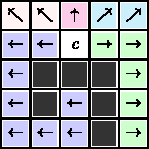
\includegraphics[width=\linewidth]{images/botea-cpd.pdf}
				\caption[Movement information in grid-based CPD.]{Movement-grid for cell $c$ in a grid-based CPD\cite{botea-cpd-2013}.}
				\label{fig:cpd}
			\end{wrapfigure}
			
			The complex part of constructing a CPD is the compression\cite{botea-cpd-2013} of the all-pairs shortest path solution.
			Uncompressed data is usually too large as the space requirement is in $\bigo{n^2}$ or even $\bigo{n^2 \log n}$ for graphs.
			A combination of compression techniques can be used to get sufficient results.
			This includes the encoding of whole areas with the same movement operations, \term*{run-length encoding} (\term*{RLE}) and the use of default values to reduce the number of explicitly stored values\cite{botea-cpd-2013}.
			Compared to uncompressed data, a compression factor of 950 was achieved for a road network.
	
\section{Geometric routing}
\label{sec:geometric-routing}

	Finding paths in a geometric domain, also called the \term{euclidean shortest path} problem, is the process of determining shortest paths without a graph but through open spaces avoiding obstacles.
	There are two main strategies for finding Euclidean shortest paths:
	Generating edges for graph-based routing or creating a shortest paths map, a structure similar to CPDs.
	
	\subsection{Visibility graphs}
	\label{subsec:visibility-graph}
	
		The first mechanism uses a standard graph-based shortest path algorithm, but the edges in the graph are generated using one of multiple possible approaches.
		One approach creates a so-called \term{visibility graph}, which is a normal graph with edges between vertices that are visible to each other.
		Or in other words, for any two $u, v \in V$ an edge $(u, v) \in E$ exists if and only if no obstacle intersects with this edge.
		A visibility graph might become very large, the worst-case regarding the size is a complete graph with $\bigo{|V|^2}$ many edges.
		
		Alternatives to the visibility graph generation are based on Voronoi diagrams or skeletonization methods.
		However, routing results on such graphs are not necessarily optimal\cite{graser-osm-open-spaces}, since a straight edge between visible vertices is the shortest possible connection.
		
		Source and destination locations must be part of the graph and can be connected with the same algorithm used to create the graph itself.
	
	\subsection{Continuous Dijkstra paradigm}
	\label{subsec:continuous-dijkstra}
	
		The second strategy, the \term{continuous Dijkstra paradigm}, creates a map of regions, similar to CPDs, starting from a source vertex $s$.
		Regions are characterized by the fact that all vertices within a region have the same predecessor on the shortest path from $s$.
		Following back the predecessors yields the shortest path from $s$ to a given location.
		This map can also be seen as a tree with root $s$ and each region as a node, which might remind one of Dijkstra's algorithm giving this approach its name\cite{mitchell-discrete-geodesic}.
		
		To precisely determine these regions, so-called \term[wavefront]{wavefronts} propagating through open spaces are used.
		A well-fitting analogy for this approach is the propagation of water waves traveling through a 2D space, folding around obstacles, colliding with each other and finally reaching the destination location.
		Collisions between wavefronts and obstacles as well as collisions between two wavefronts determine the regions' boundaries with the source of the wavefront as its predecessor.
		After detecting such a collision, the angular region of the wavefront is adjusted depending on the type of collision.
		The fundamental difficulty of this approach is the efficient detection and handling of collisions.
		Efficient algorithms are presented in \Cref{subsec:related-work-geometric-routing}.

\section{Agent-based systems and simulations}

	Simulating complex systems with numerous autonomous individuals is difficult, but using so-called \term[agent]{agents} with independent behavior and decision-making breaks down this complexity\cite{macal-introductory-tutorial}.
	Interactions between two agents and between agents and the environment are essential to this.
	
	Modeling agents can be arbitrarily complex because agents make decisions independently without any central controlling unit.
	More sophisticated agents may have a specific goal, can adapt to the environment and thus must be able to memorize and plan things.
	
	Agents usually model humans but can represent non-living things like companies or cars.
	Many simulations use pedestrians (or generally humans) as agents to better understand or utilize human behavior but other scenarios and types of agents are possible as well\cite{macal-introductory-tutorial}.

	Studying pedestrians requires a spatial environment and algorithms finding optimal paths\cite{kneidl-borrmann-hartmann-navigation,gloor-hybrid-pedestrian-routing,teknomo-millonig-routing}.
	This includes \hyperref[sec:graph-routing]{graph-based routing} but may utilize \hyperref[sec:geometric-routing]{geometric routing} as well\cite{kneidl-borrmann-hartmann-navigation}.
	In this thesis, these two concepts are combined to enhance the pathfinding component of agent-based simulations.
	
	\subsection{The MARS framework}
	
		This work aims to enhance agent-based simulations created using the framework \term*{MARS} (Multi-Agent Research and Simulation).
		MARS is a C\#/.NET framework to create and execute agent-based simulations and is developed by the eponymous research group of the Hamburg University of Applied Sciences (HAW) in Hamburg, Germany\footnote{\url{https://www.mars-group.org}}.
		The framework provides components, algorithms and tools to create tick-based simulations with multiple agents, different data layers and numerous static entities populating the environment.
		
		MARS contains several data structures and algorithms specifically for pathfinding, such as a spatial graph and the A* algorithm.
		It also contains numerous spatial indices, mathematical operations and classes to serialize the trajectories of agents.
		 
		This work is based on the MARS framework to be directly usable by simulations and uses the mentioned spatial graph and A* algorithm.
		More details on the design and implementation are given in \Cref{chap:design} and \ref{chap:implementation}.
		
	\chapter{Related work}
	\label{chap:related-work}
	
		% !TEX root = ../thesis.tex
% !TeX spellcheck = en_US

Scientific literature contains related work from many different areas, mostly from geodata, graph construction and networks as well as routing and (pedestrian) path planning.
This section gives an overview about closely related work from these areas.

\section{Graphs and networks}

	% with some assumptions like no dollinear vertices (even though these assumptions are not necessary): Constructing the visibility graph for n-line segments in O(n²) time (Emo Welzl, 1985)
	Constructing a visibility graph is an important part of this thesis.
	The construction of visibility graphs in $\bigo{n^2}$ time and space (with $n$ line segments), under the condition of no collinear coordinates and no intersecting line segments, was presented by Welzl in 1985\cite{welzl-visibility-graph}.
	A few years later, Overmars and Welzl presented two new methods reducing the space complexity to $\bigo{n}$\cite{overmars-weizl-visibility-graph}.
	Their new algorithms are based on Welzls earlier paper and the idea of a rotational sweep through neighboring vertices.
	
	% maybe, they use geom. routing to fill OSM gaps: Automatic extrapolation of missing road network data in OpenStreetMap (Funke, Schirrmeister, Storandt, 2015)

\section{Routing}

	% Shortest paths among obstacles in the plane (Mitchell, 1993)
	Shortly after Welzl and others published their work on visibility graphs, which can be used in combination with Dijkstra to find shortest paths, Mitchell presented a pure geometric method to find euclidean shortest paths around obstacles in the plain in 1993\cite{mitchell-shortest-path}.
	He used wavefronts propagating from the source towards the target vertex.
	Each origin of a wavefront can be traces back to the source giving the shortest path.
	Because this algorithm solves the \hyperref[subsubsec:single-source-shortest-path]{\term*{single-source shortest path} problem} just like the Dijkstra algorithm does on a network, this technique is also called the \term{continuous dijkstra} paradigm.
	
	% An Optimal Algorithm for Euclidean Shortest Paths in the Plane (Hershberger, Suri, 1999)
	Another approach solving the geometric single-source shortest path problem was presented by Hershberger and Suri one year later, in 1997.
	They also use the \term*{continuous dijkstra} paradigm but increase performance by introducing a special quad-tree like structure and smart subdivision of the plain.
	The result is then actually a path map allowing shortest-path request to be processed in only $\bigo{n \log n}$.
	
	% maybe: Efficient algorithms for Euclidean shortest path and visibility problems with polygonal obstacles (Kapoor, Maheshwari, 1988)

\section{Pedestrian path finding}
	
	A special case of the general single-source shortest path problem is pedestrian routing, also called pedestrian shortest-path finding.
	This problem is especially interesting since pedestrians have the maximum degree of flexibility/freedom compared to other traffic participants like bikes or cars.
	Therefore, geometric routing is a good way to find shortest-paths for pedestrians.
	
	Pedestrian path finding is, however, not only relevant for real world users, who want to know how to get from one location to another.
	Such algorithms are also used in (multi) agent simulations of pedestrian behavior.
	Scenarios in such simulations are for example evacuation or crowd behaviors.
	The area of pedestrian path planning and simulations is divided into two strategies: Network and field based path finding\cite[2]{hartmann-geodesic}.
	Work from both strategies will be covered here.
	
	\subsection{Field based navigation}
		
		% online routing: A Navigation Algorithm for Pedestrian Simulation in Dynamic Environments (Teknomo, Millonig, 2007)
		Teknomo and Millonig created a dynamic algorithm which does not pre-compute the path with one of the above mentioned approaches\cite{teknomo-millonig-routing}.
		This is interesting, since the probably most common and naive approach is to pre-compute the route used by an agent within a simulation.
		The term \enquote{dynamic} refers to the fact, that real world pedestrians often only consider the near neighborhood within their path planning.
		Even if a person knows the hole area, dynamic changes (closed doors, construction work, crowds blocking the way) can still occur at any point in time.
		Therefore, such dynamic considerations can be one aspect to make simulations more realistic.
		
		% maybe: pure geometric/geodesic approach with navigation fields: https://iopscience.iop.org/article/10.1088/1367-2630/12/4/043032/pdf
		The above mentioned dynamic routing by Teknomo and Millonig has strong similarities to approaches based on potential fields, like the dynamic path finding from Hartmann, 2010\cite{hartmann-geodesic}.
		He proposed a mechanism using vector fields in a cellular automaton model with hexagonal cells.
		Interestingly, this method can be interpreted as wavefronts, like in Mitchells algorithm described above, propagating through the vector field\cite[4]{hartmann-geodesic}.
			
		% unified pedestrian routing (they use the above navigation field graph generation): A Unified Pedestrian Routing Model for Graph-Based Wayfinding Built on Cognitive Principles (Kielar, et al. 2017)
	
	\subsection{Graph generation for pedestrian navigation}
	
		An alternative to field based approaches are graph based ones, where a graph is constructed and then used in navigation.
		The construction can be based on potential fields but also on the above mentioned \term*[visibility graph]{visibility graphs}.
		
		In fact, Gloor, Stucki and Nagel presented a pedestrian navigation model and a comparison of these two strategies regarding their performance\cite{gloor-hybrid-pedestrian-routing}.
		They developed this model for a pedestrian simulation in the Alps, where a hiking network should be enhanced with additional navigation information.
		Two approaches were presented: A potential field based method, which is used in navigation when needed, and a visibility graph, which is merged into the existing hiking network.
		The visibility graph strategy strongly relates to this thesis.
		For the performance evaluation, they used an evacuation scenario.
		The results showed, that both navigation mechanisms are comparably fast.
		
		A very similar approach, at least with visibility graphs as a base, was chosen by Kneidl, Borrmann and Hartmann to produce a sparse navigation graph\cite[5]{kneidl-borrmann-hartmann-navigation}.
		They chose the construction of a visibility graph over generalized Voronoi diagrams for more realistic edges.
		
		Another interesting paper on enhancing existing navigation graphs, like Gloor, Stucki and Nagel did, was presented in 2016 by Anita Graser by integrating visibility graph edges into the existing OSM data model\cite{graser-osm-open-spaces}.
		Again, the visibility graph was the preferred method of producing edges.
		Considered and discussed alternatives here were two skeletonization methods and a simple grid places over open spaces.
	
	\chapter{Design}
	\label{chap:design}
	
		% !TEX root = ../thesis.tex
% !TeX spellcheck = en_US

This chapter covers the design of the implemented hybrid routing algorithm.
First, the overall context is presenting specifically the requirements and constrains of the algorithm.
Second, details on the decisions regarding the routing strategy and general design are presented.
Finally, an overview of the separate components is given as well as a description on the deployment of this algorithm.

\section{Requirements and constrains}

	% Used by agents for wayfinding
	The primary goal of the hybrid routing algorithm is to provide a path planning algorithm that is integrated into the MARS framework and offers more accurate paths compared to common graph based algorithms on road datasets, thus, enhancing agent based simulations.
	Such a major goal implies several constrains on the architecture and design of the software.
	
	\subsection{Requirements}
	
		Functional requirements of the resulting software can be formulated quite easily, since this is not a large commercial product.
		The hybrid routing algorithm should determine an optimal path between two locations following ways and traversing open spaces while avoiding obstacles.
		A configurable weight function should be used to assign a weight to each edge in order to find the path with the minimum weight.
		Processing of geospatial data must consider existing road network data as well as obstacles, which are features that will be avoided on paths traversing open spaces.
		It must be possible for the shortest path to alternate between segments following roads and open spaces.
		
		More complex and time consuming are the quality requirements.
		Because this is not part of a commercial software development, these requirements are not part of any tender and were not even formulated.
		Nonetheless, they exist and consist of the following aspects.
	
		The largest quality requirement in terms of effort is performance.
		It affects large parts of the software architecture since the resulting algorithm, despite its complexity, should ideally have a negligible impact on the overall performance of a simulation compared to current graph based routing approaches.
		Routing algorithms and engines often consist of two steps: preprocessing and answering routing queries.
		In order to create fluent and fast simulations, the performance of answering numerous routing requests must be as good as possible.
		The time needed for preprocessing is of less importance.
		
		A rather obvious requirement is the correctness of resulting routes.
		Answers of routing queries must return the shortest route according to a given weight function.
%		Even when using an approximation algorithm to determine shortest paths, the results can be checked against all other possible paths to verify the optimality of the resulting path.
		
		Another quality requirement is the closeness of the resulting routes to real pedestrian behavior.
		Unfortunately, this can hardly be measured without having extensive data of real world pedestrians in real world locations.
		Ideally, the trajectory of a calculated route should be identical to a real world pedestrian trajectory.
		It should at least make sense to an observer without additional knowledge of the real world location.
		The coordinates of waypoint on the calculated and on real trajectories must not be exactly the same, since real pedestrian behavior is not part of the shortest path calculations but is instead a task for realistic agent modeling.
		Such behavior includes for example a typical minimum distance kept to obstacles or a minimum radius of walked curves.

		Next to the domain specific requirement, the overall code itself should of course be well documented and tested.
	
	\subsection{Constrains}
	\label{subsec:constrains}
		
		% Well integrated into MARS and NTS, no new dependencies
		One major constraint is the integration of final algorithm into the \term*{MARS} framework to make the use as easy as possible and to centralize the code base for better maintenance.
		This means the programming language will be C\# and additionally, because MARS uses the geospatial framework \term{NetTopologySuite} (\term*{NTS}) as basis for all major geospatial operations, this algorithm will be based on NTS.
		
		The planned integration into another code base affects the management of dependencies.
		On the one hand, the amount newly introduced dependencies should be kept to a minimum.
		On the other hand, using only libraries on which MARS depends as well is not always possible due to version mismatches.
		However, the latter case can be avoided and should disappear with future dependency updates.
	
\section{Combination of routing algorithms}
\label{sec:combining-routing-algorithms}

	This section describes the core aspect of this thesis:
	The decision of a strategy to combine graph and geometric based routing algorithms.
	A decision on this \enquote{merge} strategy to be implemented is crucial to the design and architecture of the application.
	
	In the following, four approaches are discussed of which the last is considered to be the most promising, which was therefore chosen to be implemented.
% STIMMT NICHT:	The first three are using any normal graph based routing algorithm, like A* or Dijkstra, in combination with the geometric continuous Dijkstra paradigm.
%	Only the last and further pursued approach uses visibility graphs for routing.
	
	% Ad-hoc creation of edges by stopping A* and continuing with wavefront algorithm
	\subsection{Approach candidate 1: Ad hoc generation of edges}
	
		The idea of an ad hoc generation of edges is the following:
		Whenever the graph routing algorithm reaches a road junction, it's paused and the continuous Dijkstra algorithm is started.
		No destination vertex is defined, which means the geometric routing will be stopped after the furthest wavelet reached a certain distance.
		The continuous Dijkstra approach actually creates a shortest path map, so the shortest paths to all reached vertices are calculated.
		All shortest path edges are then added to the graph for the paused graph based routing algorithm.
		
		A real world example for this approach would be a pedestrian walking down a road, stopping at a junction to decide where to go and choosing the option to cross a park for a shortcut before continuing to follow the roads again.
		Doing the shortcut was not planned but an ad hoc decision, just as the algorithm would do.
		
		The advantage of this approach is the realistic behavior of pedestrians not planning the route in beforehand.
		In fact Teknomo and Millonig introduced a routing mechanism for agent based simulations with the assumption of little to no apriori knowledge of agents about their environment \cite{teknomo-millonig-routing}.
		This approach would therefore implement their assumptions on agents behaviors.
		
		One disadvantage is a relatively high complexity since no standard algorithm from frequently used software frameworks support a pause functionality, so any routing algorithm has to be manually adjusted or implemented from scratch.
		
		Also this approach will likely cause performance issues.
		When using Dijkstra as graph based routing algorithm, $\bigo{|V|}$ many vertices are visited, which leads to $\bigo{|V|}$ routing requests using the geometric continuous Dijkstra algorithm.
%		Because a simple caching of the shortest path map is not possible, at least not without a smart and complex caching strategy, this decreases the runtime of the whole routing process significantly.
		Even when using the continuous Dijkstra approach from Hershberger and Suri \cite{hershberger-suri} with only $\bigo{n \log n}$ time requirement, the number $n$ of vertices in obstacles is expected to be much higher than the size of $V$ resulting in a somehow quadratic runtime.
		Caching the shortest path map using a \term*{CPD} (see \cref{subsubsec:cpd}) would be possible but would also increase complexity during query time and reduce performance during preprocessing time.
		Storing precomputed edges in a simple map would reduce complexity, still increase query time but also still reduce precomputation time.
		
		The ad hoc idea of this approach yields no significant advantage compared to a preprocessing.
		Therefore, this approach was not further pursued.
		
%		Another aspect against this approach is the fact that an ad hoc generation of edges will probably not change the resulting shortest path in comparison to a precomputation of these edges.
%		An argumentation for the correctness of this hypothesis can be sketched as follows.
		
%		Assume that the ad hoc generation starts at each road junction vertex $j$ and stops when a certain condition is fulfilled (for example only generating paths of a certain length).
%		When the graph routing algorithm reaches an unvisited junction vertex $j$ from some other vertex $v$, it either used a road edge or preprocessed edge to get there. Therefore, the following two cases exist:
%		\begin{itemize}
%			\item In case a preprocessed edge was used, then the shortest path from $v$ to $j$ would be identical when using a completely preprocessed graph containing this exact edge $(v, j)$.
%			\item In case a road edge was used to get to $j$, then there are two sub-cases.
%			\begin{itemize}
%				\item In case the road edge was in deed the optimal path to $j$, it would have been used in a preprocessed graph as well.
%				\item In case the road edge was not the optimal path, then the ad hoc generation stopped before reaching $j$ (due to the distance or any other stopping condition) and the edge $(v, j)$ was never added.
%			\end{itemize}
%		\end{itemize}
%		Even though, this is not a formal proof, generating a preprocessed graph and using a normal routing algorithm is probably as least as good as using the ad hoc generation approach.
	
	% Concurrent routing: Use A* and wavefront in parallel and merge the results
	\subsection{Approach candidate 2: Concurrent routing}
	
		A different approach would be two concurrent routing queries, one on the normal road graph and one using a visibility or otherwise generated graph.
		Having the two shortest paths, they could be merged into one path, which results in segments with alternating source graph.
		To merge them, first the intersection points need to be determined and then the better segments have to be chosen based on a weight function.
		
		The most prominent advantage is the simplicity of the routing requests, since known routing algorithms could be used.
		Therefore, it would be rather simple to implement and speed up techniques could be used.
		
		However, there are two major disadvantages.
		First, it is uncertain that the two paths are actually intersecting at any point.
		Second, even if they are intersecting, too few intersections on a long route result in suboptimal paths, because the longer a segment gets, the less accurate the weighting becomes.
		Only if the two routes are intersecting frequently enough, the selection of segments based on the weight function could actually result in good routes.
	
	% Concurrent routing for segments (e.g. start new routing calls every 100m)
	\subsection{Approach candidate 3: Concurrent routing on smaller segments}
	
		This approach is very similar to the one above, but it tries to fix the uncertainty of intersections between the two resulting paths.
		Multiple ways are conceivable to ensure that there are enough intersections or to otherwise guarantee that segments are small enough to be merged.
		
		One way is to stop the routing after a certain distance stopping at the next available vertex.
		After stopping for the first time, there are two such vertices, one where the road network based routing stopped and one where the routing on the generated graph stopped.
		From each vertex, two new routing queries start and stop again after a certain distance.
		This continues until one query reaches the destination.
		On the one hand, this would guarantee small enough segments for later merging, on the other hand, this results in $\bigo{2^n}$ many routing queries.
		Even though each query is short, this approach would probably, even with the help of heuristics or other helping mechanisms, not scale very well.
		
		A different approach to obtain smaller segments would be to first get the shortest path on the road graph.
		Having this path, it is split up into $n$ segments of certain length connecting the vertices $v_0, v_1, ..., v_n$ with $v_n$ being the destination.
		In a next step, shortest paths from each vertex to following vertices are calculates.
		Meaning from $v_i$ paths to $v_{i+1}, v_{i+2}, ..., v_n$ are determined, which unfortunately results in $O(n^2)$ many routing queries.
		Finally, all these paths on the generated graph can be merged together with the query result of the road graph to form a new intermediate graph..
		Finally, one last routing query on this intermediate graph is performed to get the final optimal routing result by using a weight function analogous to the previous approach.
		Instead of an intermediate graph, other combinatorial approaches can be used as well since the shortest path problem can be solved using linear programming \cite{handler-zang-lp-duality}.
		
		There are probably more possible ways to ensure a sufficient amount of segments or intersections, however, this idea was not further pursued.
		
		Unfortunately, both approaches have a worse time complexity than any popular routing algorithms including pure geometric routing.
		Even though the second idea might work well for appropriate segments lengths, the complexity and definite time overhead make it an unfavorable choice.
	
	% Merge of networks
	\subsection{Approach candidate 4: Merge an existing network with a visibility graph}
	
		Previous approach candidates tried to first calculate shortest paths and then merge their results.
		This last approach, which is the currently used one, first merges a generated visibility graph with an existing road graph.
		The actual merge operation is very simple:
		Whenever a road edge and a visibility edge intersect, split the edges, create a new vertex at the intersection point and connect the split edges accordingly.
		
		Even though, this approach is simple and still fast, the main disadvantage is the graph size.
		A visibility graph is large and in most cases it will contain many more edges than the road graph, which negatively affects the routing performance.
		
		Another disadvantage is the time complexity of the merge operation.
		All edges have to be considered and, depending on the number of intersections, edges might be processed multiple times (e.g. one visibility edge might intersect with all road edges).
		This leads to at most $|E_R| \cdot |E_V|$ many merge operations for the routing graph edges $E_R$ and visibility edges $E_V$.
		Complete graphs have the highest number of edges and therefore the highest number of intersections, which gives the upper bound of $\bigo{|E|^2}$ for the merge operation given all edges $E$.
		Fortunately, road networks are very sparse and often have a node degree between three and six \cite{zhao-analysis-osm-bejing}\cite{boeing-osmnx}, resulting in a probably much better runtime behavior in practice.
		\todo[inline]{Maybe analyze this myself for e.g. Germany?}
		\todo[inline]{Link to possible optimizations discussed in later chapters}
		
		Despite the disadvantages of this approach, I considered the advantages to be more important.
		As already mentioned, this strategy is not only simple and fast, compared to some time complexities mentioned previously, but it also allows the use of speed up methods for routing queries.
		Moreover, the resulting path is definitely optimal, based on the given weight function, and no complex postprocessing is needed.
		
		Taken all aspects into account, this strategy seemed to be the simplest and most promising with the least disadvantages.
		It was therefore chosen to be implemented.

\section{Design decisions}
\label{sec:design-decisions}

	With the choice of the merge strategy being the approach of combining two different routing algorithms, several design decisions were made.
	Some decisions did not influence the overall architecture and were just made to enhance performance or simplify the implementation, this section only covers fundamental decisions relevant for the overall architecture.
	\Cref{chap:implementation} covers those decisions that are independent of the overall architecture.
	
	In this work I implemented the visibility graph without the use of algorithms presented in the according \hyperref[subsec:related-work:visibility-graph]{related work section}.
	None of the existing approach would have been easy to implement without problems.
	Details on these problems and the exact reasons that led to the decision of a custom implementation are presented in this section.
	
	\subsection{Requirements and considerations for the visibility graph creation}
	
		One key requirement for the visibility graph creation is the ability to work in arbitrary obstacles, which primarily includes the fundamental point, linestring and polygon geometries.
		To work with arbitrary real world datasets, assumptions about the collinearity, position of obstacles and intersections between them cannot be made.
		
		An important special case arises for linestring obstacles consisting of more than two points.
		Simply determining visibility edges to and from both sides of the linestring would result in shortest paths leading right through it.
		Of course, this is the opposite of the desired behavior of a shortest path leading \emph{around} the linestring.
		The same situation would arise with obstacles, including polygonal ones, touching in a single node.
		
		Since the visibility graph is solely used to determine shortest paths, some assumptions and optimizations can still be made.
		However, these considerations are not relevant for the overall architecture and are therefore covered in \cref{sec:visibility-graph-creation}.
		
		A core aspect of the routing algorithm is the reachability of arbitrary locations not located on the graph.
		Adding visibility edges after the complete graph has been created must therefore be possible.
		Implementing this is necessary regardless of the chosen algorithm for the visibility graph creation.
		
		One very important reason why no highly optimized approach was chosen and also why only a limited amount of effort went into the optimization of my own approach is the fact that generating the graph is separated from its use.
		Far more significant is the routing behavior itself as it directly affects the simulation time.
		Creating the graph in a preprocessing step has, especially when persisting the graph for multiple uses, no direct effect on the simulation.
		
		All these requirements and considerations, including problems and efforts outlined below, lead to the decision of implementing a simple graph generation approach with some easy but effective optimizations.
	
	\subsection{Suitability of existing approaches}

		The largest and most influential design decision was the decision against an approach from the literature as presented in \cref{subsec:related-work:visibility-graph}.
		Several approaches from the literature have either restrictions on the geometric structures or assume that a certain preprocessing of the data was already performed.
		
		The approach by Welzl \cite{welzl-visibility-graph}, for example, explicitly assumes that there are not collinear vertices, i.e. at least three vertices forming a straight line.
		It may seem unlikely at first that collinear vertices occur in real world datasets, but in fact, at least in OpenStreetMap, it is very common to align touching buildings and other straight obstacles like walls.
		
		An optimization of Welzls approach, by Overmars and Welzl \cite{overmars-weizl-visibility-graph}, only works on non-intersecting line segments.
		Real world data is unfortunately too diverse to fulfill this criterion as polygons, longer linestrings and other more complex data structures exist.
		Preprocessing the data, i.e. cutting all geometries into such non-intersecting line segments, would cause new special cases to solve.
		For example, cutting a polygon into line segments would add visibility edges within the former polygon, which needs to be avoided e.g. by storing metadata about the relations of these line segment to each other.
		Handling all those special cases, preventing unwanted edges and still using the approach by Overmars and Welzl would be possible but would also increase the complexity of their approach.
		
		Another approach with the limitation of no collinear vertices was the plain-sweep algorithm by Ghosh and Mount \cite{ghosh-output-sensitive-vgraph}.
		Next to the limitation on collinear vertices, they assume x-coordinates to be unique, which, even though it is very likely fulfilled in real world datasets, would need to be handled as well.
		
		Kapoor and Maheshwari presented a visibility graph creation as well \cite{kapoor-shortest-path-vgraph} but assumed a triangulation of the open space between the obstacles.
		Such a triangulation can be done quite fast, algorithms with time complexities of $\bigo{n \log{n}}$ and better are known \cite[58-60]{de-berg-computational-geometry}, but libraries such as MARS or the NetTopologySuite do not implement this.
		They only provide triangulation methods for polygons but not for the space between them.
		Implementing an algorithm for this task would be needed in addition to the visibility graph creation itself.
		
		Probably all approaches from the literature would work but preprocessing, restrictions on the input data or adjustments to the approaches would be necessary.
		Since this work focuses more on the overall concept of a hybrid routing algorithm, the choice on the graph generation algorithm was of less importance.
		Therefore, the implementation is much simpler and independent of the above mentioned approaches.
	
\section{Components}
\label{sec:components}

	% Generator classes, HybridVisibilityGrahp class and helper functions
	Since this works resides in a rather technical and algorithmically oriented context, there are not many separate components needed to implement a hybrid routing approach.
	One component if the so called \term{hybrid visibility graph}, which is the final output graph consisting of the merged road and visibility edges.
	These edges are created by the according generator component.
	Finally, the merging and creation of the hybrid visibility graph takes place in a third component.
	
	\begin{figure}[h]
		\begin{figcenter}
			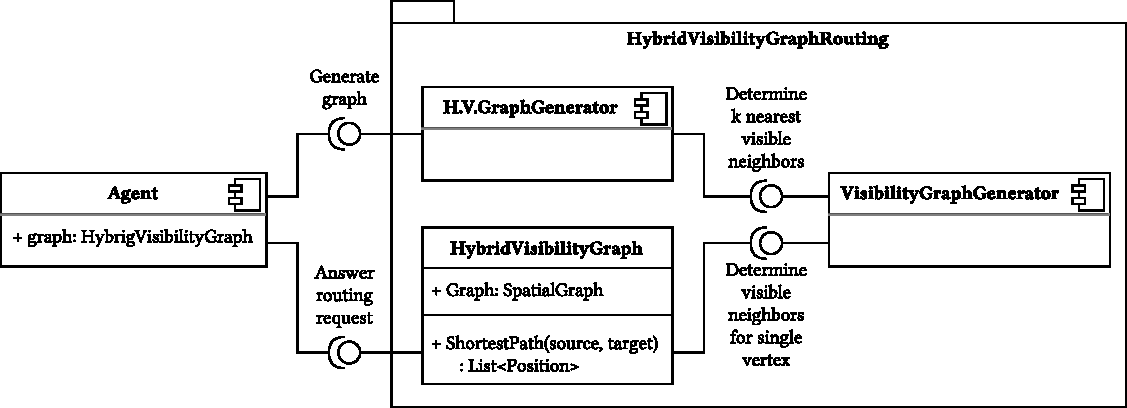
\includegraphics[width=\textwidth]{images/components.pdf}
		\end{figcenter}
		\caption{The components and usages of interfaces of the resulting implementation.}
		\label{fig:components}
	\end{figure}
	
	The first step for a consumer of the system, e.g. an agent based simulation, is to generate the hybrid visibility graph.
	Hence, the \texttt{HybridVisibilityGraphGenerator} (abbreviated as \enquote{H.V.GraphGenerator} in \cref{fig:components}) presents a public interface for this task.
	The result of the graph generation is an instance of the \texttt{HybridVisibilityGraph} class offering public methods to answer shortest path requests, such as the \texttt{ShortestPath} method returning a list of positions (i.e. coordinates) representing the shortest path between two input coordinates.
%	More details on the graph generation can be found in \cref{sec:graph-generation}.
	
	For convenience and due to required preparations, routing queries are put to the hybrid visibility graph.
	To fulfill the overall concept of this work, it must be possible to start and end at arbitrary locations, thus, there is no guarantee that the source and destination locations of the query are on any vertex in the graph.
	Therefore, the hybrid visibility graph has to temporarily connect these locations to the graph.
	This is done by determining all visible neighbors of the source and destination locations and then merging the resulting edges to the underlying graph.
	To perform this task, the hybrid visibility graph uses the interface of the \texttt{VisibilityGraphGenerator} to determine visibility neighbors of a single vertex.
	\Cref{sec:answering-queries} covers the process of answering routing queries in more details, including the clean up step that is performed after the shortest path has been found.

\section{Deployment view}

	% published in MARS
	\todo{Publishing in MARS}


	
	\chapter{Implementation}
	\label{chap:implementation}
	
		% !TEX root = ../thesis.tex
% !TeX spellcheck = en_US

This section describes more implementation details of the previously described approach.
First, an overview of the algorithm with a short description of used frameworks and technologies is given.
After that, the main sections of this chapter show details of each algorithmic step.

\section{Algorithm overview}

	\subsection{Frameworks and technology}
	
		As mentioned in \cref{subsec:constrains} about the constrains, the used programming language is C\# due to the dependency to the MARS framework.
		The MARS framework is based on the widely used C\# library \term{NetTopologySuite} (\term*{NTS}), which contains numerous data structures, algorithms and helper function to handle and process geospatial data.
		
		The NTS was primarily used for basic data structures like features and geometries.
		Writing data to files is also done using NTS functions to serialize the geospatial data into GeoJSON files.
		
		The \term*{MARS} framework was also used for basic data structures, like the \texttt{Position} class.
		However, higher level structures like quadtrees and mathematical calculations were used as well.
		
		Not all data structures and algorithms already existed to create the hybrid routing graph.
		Most notably, a fast line intersection check was implemented as well as a bin based index structure.
		Several other helper functions and simpler structures, like a separate class for vertices, were added as well.

	\subsection{Early implementation based on the continuous dijkstra paradigm}
	
		An early implementation was not creating a visibility graph but instead it was based on the \term*{continuous dijkstra} paradigm with wavelets propagating through open spaces.
		However, there were two reasons why this first approach was replaced by a visibility graph based algorithm.
		
		The first reason was a bad performance.
		Early stages of the continuous dijsktra approach used a very naive and simple implementation without optimizations mentioned in recent literature on this topic.
		Before investing larger efforts into the implementation of a more complex approach, like the one presented by Hershberger and Suri\cite{hershberger-suri}, a simple preprocessing was introduced and lead to a major performance enhancement.
		This perprocessing determined the visibility between all vertices, which was later used to create events for the collision between wavelets and vertices.
		Such predetermined visibilities are the core of a visibility graph, thus moving to an actual visibility graph based approach was not a big step.
		
		The second reason to actually move towards a visibility graph was the difficulty and the disadvantages of combining the network based routing with the continuous dijkstra algorithm implemented so far, as described in \cref{sec:combining-routing-algorithms}.
		Therefore, the decision fell in favor of implementing and optimizing the creation of a routable visibility graph.
	
	\subsection{Chosen approach and potentially faster known algorithms}

		% Maybe this whole subsection is part of a later discussion?
		Due to the step by step development by turning the former continuous dijkstra preprocessing into a visibility graph generator, the implemented approach does not follow algorithms described in the literature.
		The performance of this implementation, as shown in \todo[inline]{link to chapter}, is still enough for practical use, but a well designed and fast algorithm, like the one presented by Overmars and Welzl \cite{overmars-weizl-visibility-graph} or the one by Ghosh and Mount \cite{ghosh-output-sensitive-vgraph}, would clearly increase performance.
		However, this performance enhancement would only affect the generation of a visibility graph and not the performance of the routing queries.
			
	\subsection{Algorithm steps}
		
		As describes in \cref{sec:components}, the \texttt{HybridVisibilityGraphGenerator} class provides a factory method to create a \texttt{HybridVisibilityGraph} from a given collection of features.
		This factory method consists of the following top level steps.
		\todo[inline]{more?}
		
\section{Visibility graph creation}
		
	\subsection{Step 1: Obstacle filtering and feature preprocessing}
	\label{subsubsec:step-1-preprocessing}
			
			First the features are filtered to get all relevant obstacle features, which are of arbitrary shape.
			For performance reasons, multi-geometries, like \texttt{MultiPolygon} are split up into their separate geometries.
			This is not only unproblematic for \texttt{MultiLineString} but also for \texttt{MultiPolygon} features, since holes in a polygon are not reachable in the first place and unwrapping the \texttt{MultiPolygon} will not change this.
			% TODO Better formulation?
			Another task within this first step is the triangulation of all polygonal shapes.
			The main reason is a better performance for intersection checks, which is an important task of creating a visibility graph.
			
	\subsection{Step 2: Determining $k$ nearest visible neighbors}
			
			After having all preprocessed obstacles, the main task of the visibility graph creation is performed, namely determining all $k$ many visible neighbors.
			Determining all visible neighbors would also be possible, but this parameter is an easy way to increase performance with the downside of not having all possible edges in the final routing graph.
			
			\subsubsection{Overview and terminology}
			
				Before describing the details on determining the $k$ nearest neighbors, there are some terms that need to be defined.
				
				\begin{description}
					\item[\term*{visibility neighbor}] Sometimes also just \emph{visible neighbor} is a vertex $u$ that is visible from the currently processed vertex $v$.
					\item[\term*{obstacle neighbor}] This is a vertex $u$ with an existing edge to or from the currently processed vertex $v$. In other words, $u$ is visible from $v$ but via an existing obstacle edge.
					\item[\term*{shadow area}] This is an angle area that starts at a certain distance, for example \enquote{10° to 20° with a minimum distance of 30 meter}.
				\end{description}
			
				\noindent The performed steps of determining the visible neighbors are the following, more details are given in the section below.
				\begin{enumerate}
					\item Get the obstacle neighbors for each vertex.
					\item For each vertex $v$, determine its visibility neighbors as follows.
					\begin{enumerate}
						\item For each other vertex $u$, do the following:
						\begin{enumerate}
							\item Is $u$ in any shadow area? If so, which means $u$ is not visible, move to the next other vertex. Continue otherwise.
							\item Query all obstacles between $v$ and $u$.
							\item Create and store the shadow area of each such obstacle $o$.
							\item Mark $u$ as visibility neighbors if $u$ is still not in any shadow area and a line segment from $v$ to $u$ intersects with none of the above queries obstacles.
						\end{enumerate}
						\item Sort visibility neighbors into bins based on the obstacle neighbors.
					\end{enumerate}
				\end{enumerate}
			
			\subsubsection{Parameter $k$}
			
				The $k$, however, is not just a single parameter, but rather consists of two separate values:
				The number of bins and the number of maximum neighbors per bin.
				Each bin covers a certain angle area of each vertex, for example for a bin count of 36, each bin would cover a 10° area.
				Without this subdivision of the neighbors, it is possible to only have edges to complex and close objects but no edges to obstacles further away.
				
				An example for this would be a large and open park where the $k$ nearest neighbors are probably all at the side of the park where the currently processed vertex is, even though the far away other side of the park is clearly visibly.
				This subdivision into bins ensure that there will definitely be connections to the other side of the park.
			
			\subsubsection{Determining obstacle neighbors}
				
				Determining the obstacle neighbors is relatively simple and straight forward.
				Each coordinate $c$ of an obstacle $o$ is processed by looking at the previous and next coordinates $c_p$ and $c_n$ on that obstacle, which are the potential neighbors.
				If the line segment $(c, c_p)$, for $c_n$ respectively, does not intersect with any obstacle, it is considered an obstacle neighbor.
				
			\subsubsection{Shadow areas}
			
				Shadow areas are a simple method to quickly determine vertices that are definitely not visible to each other.
				The idea of shadow areas is the following:
				Let $v$ be the currently processed vertex and think of it as a light bulb illuminating its surroundings.
				An obstacle $o$ casts a shadow outwards and everything within this shadow is definitely not visible from $v$.
				
				The distance from which everything within the angle area of the shadow is definitely not visible from $v$, is determined by the two bounding vertices (marked in red in \cref{fig:shadow-area}).
				These bounding vertices determine the angular range and the furthest of these two determines the minimum distance of the shadow area.
				
				Keeping track of these shadow areas for each vertex significantly improves performance.
				\todo[inline]{conrete numbers?}\todo[inline]{Reference to BinIndex below or other used data structure (s. TODO below)}
				% NetworkRoutingPlayground->Jungfernstieg dataset with 7916 vertices: ~7.3s with and 67s without shadow areas -> speed up of factor ~9
				% Hamburg inner city dataset with 67819 vertices: 382s with and ~31000s without shadow areas -> speed up of factor ~81
				
				\begin{figure}[h]
					\begin{center}
						\begin{tikzpicture}
							\def\angle{20}
							\def\boundingVertexDistance{3}
							
							\tikzDot[label=$v$]{(0,1.5)}{v}
							\coordinate (shadow-arc-top)				at ($(v) +( \angle:\boundingVertexDistance)$);
							\coordinate (shadow-arc-bottom)				at ($(v) +(-\angle:\boundingVertexDistance)$);
							\coordinate (shadow-arc-top-end)			at ($(v) +( \angle:5.75)$);
							\coordinate (shadow-arc-bottom-end)			at ($(v) +(-\angle:5.75)$);
							\coordinate (shadow-arc-top-faded-end)		at ($(v) +( \angle:6.5)$);
							\coordinate (shadow-arc-bottom-faded-end)	at ($(v) +(-\angle:6.5)$);
							
							% Gray area
							\filldraw[lightgray] 
								(shadow-arc-bottom) arc [start angle=-\angle, delta angle=2*\angle, radius=\boundingVertexDistance] --
								(shadow-arc-top-end) --
								(shadow-arc-bottom-end) --
								cycle;
							\draw[gray]
								(shadow-arc-bottom-end) --
								(shadow-arc-bottom) arc [start angle=-\angle, delta angle=2*\angle, radius=\boundingVertexDistance] --
								(shadow-arc-top-end);
							
							\draw[dotted] (v) -- (shadow-arc-top);
							\draw[dotted] (v) -- (shadow-arc-bottom);
							
							% Faded gray area
							\filldraw[draw=none,lightgray,path fading=east]
								(shadow-arc-top-faded-end) --
								(shadow-arc-top-end) --
								(shadow-arc-bottom-end) --
								(shadow-arc-bottom-faded-end) --
								cycle;
							\draw[gray,path fading=east] (shadow-arc-top-end) -- (shadow-arc-top-faded-end);
							\draw[gray,path fading=east] (shadow-arc-bottom-end) -- (shadow-arc-bottom-faded-end);
							
							% Obstacle 1
							\tikzDot[red]{(shadow-arc-top)}{o10}
							\tikzDot{(3.5,2)}{o11}
							\tikzDot[red]{($(v) +(-\angle:1.2)$)}{o12}
							\node[above right = 0.5 and 1 of o12] {$o_1$};
							
							% Obstacle 2
							\tikzDot[label=right:$v'$]{(3.5,1.35)}{o20}
							\tikzDot{(3.5,-0.25)}{o21}
							
							% Obstacle 3
							\tikzDot[label=right:$v''$]{(2.1,1.1)}{o30}
							\tikzDot{(2.1,-0.5)}{o31}
							
							\node[darkgray] at (4.65,1.5) {\huge$S$};
							
							\draw (o10) -- (o11) -- (o12) -- (o10);
							\draw (o20) -- node[right] {$o_2$} (o21);
							\draw (o30) -- node[left] {$o_3$} (o31);
						\end{tikzpicture}
					\end{center}
					\caption{Shadow area $S$ cast by obstacle $o_1$ seen from vertex $v$. The vertex $v'$ of obstacle $o_2$ is not visible from $v$ since it lies inside the shadow area. The two red vertices of obstacle $o_1$ are the bounding vertices determining angle range and distance of $S$. Not that $v''$ is not visible from $v$ as well even though it is not inside the shadow area.}
					\label{fig:shadow-area}
				\end{figure}
				
			\subsubsection{BinIndex data structure}
			
				The \texttt{BinIndex} class implements a simple index structure to store and access intervals.
				It contains $n$ many bins of which each covers a certain range and consists of a linked list.
				When an item is added, it is added to each bin intersecting with the range of the item.
				Due to the list as underlying data structure for the bins, queries can be answered in $\bigo{m}$ time for $m$ many items in the index.
				
				The NetTopologySuite offers several indices specifically made for intervals, namely the \texttt{BinTree} and \texttt{SIRtree}, of which the latter one is static and does not allow insertions after the first query was made.
				Even though these two structures are tree based and theoretically offer a logarithmic query complexity compared to the linear complexity of the \texttt{BinIndex}, the simple and list based \texttt{BinIndex} is significantly faster even for larger datasets with tens of thousands of vertices.
				It is thinkable that the logarithmic complexity is useful for huge datasets with millions of vertices, but that has not been tested.
			
			\subsubsection{Intersection checks}
			
				All intersections are checked using own implementations no not rely on the generalized and therefore slower intersection checks of the NetTopologySuite.
				In fact, there are two types of intersection checks implemented:
				One check for intersection between two arbitrary line segments and one checks if a point lies within a triangle.
				This triangle check is used for closed obstacles, which got triangulated during \hyperref[subsubsec:step-1-preprocessing]{preprocessing}.
				
				The line segment intersection check uses a cross product based approach described in \emph{Introduction to algorithms} by Thomas H Cormen et al \cite[1018]{cormen-introduction-to-alg}.
				
				Checking if a point lies inside a triangle is done by a barycentric collision check.
				This method creates a barycentric coordinate system where each coordinate consists of three values $\lambda_1$, $\lambda_2$ and $\lambda_3$ for each corner vertex of the triangle.
				Due to the properties of this coordinate system, a point $p$ is inside the triangle when the condition $0 < \lambda_i < 1$ hold for each of the three values.
				Even though it sounds complex to create a whole coordinate system for a single collision check, this method only uses a few basic arithmetic operations and is therefore very fast.
			
			\subsubsection{Sort resulting visibility neighbors into bins}
			
				A naive approach to create a visibility graph would be to create edges between vertices that see each other.
				This would make routing through line based obstacles possible, which is of course not correct.
				It must therefore be known which visibility relations are between which obstacle neighbors.
				Knowing this enables the graph generation to distinguish between all the edges and results in correct routing results.
				More on this in the \cref{subsec:step-3-graph-creation} below.
				
				Each of the resulting bins of a vertex $v$ covers the area between two adjacent obstacle neighbors.
				All visibility neighbors are sorted into these bins, which is a simple and easy process.
			
	\subsection{Step 3: Graph creation with visibility edges}
	\label{subsec:step-3-graph-creation}
		
	\subsection{Step 4: Merging a road network into the visibility graph}

\section{Answering shortest path queries}
	
	\chapter{Evaluation}
	\label{chap:evaluation}
	
		% !TEX root = ../thesis.tex
% !TeX spellcheck = en_US

The implementation of the hybrid routing algorithm was evaluated regarding performance and usefulness, which is covered in this chapter.
For both evaluation aspects, method and design details are given followed by the respective results of the evaluations.

\section{Performance evaluation}

	The performance evaluation uses different datasets to measure graph generation and routing times.
	Each of these two steps is measured more fine-grained by measuring the execution times of separate method calls.
	The datasets have different properties and sizes and consist of artificial and real-world data.

	\subsection{Methods \& Measurements}

		\subsubsection{Collected data}
		
			The collected data consists of time measurement, many of them on the level of separate methods.
			Also, the amount of data is measures, namely the number of edges and vertices at various steps in the process.
			
			As a result, two CSV files are written per dataset containing measurement data for the import (including graph generation) and routing.
			The measurement for the routing requests also contains information about the lengths of the routes, especially beeline and actual route distances.
			
			% TODO table with all columns of the measured data including a description and example value?
		
		\subsubsection{Datasets}
		\label{subsubsec:eval-datasets}
		
			There are multiple categories of datasets that were used.
			Pattern-based datasets are created using a pattern, e.g. a set of rectangles, repeated numerous times to create datasets of various sizes.
			OSM-based datasets use differently sized extracts from OpenStreetMap.
			While the OSM-based datasets contain obstacles and roads (except in the \enquote{without roads/obstacles} datasets), the pattern-based datasets do no contain any roads.
			
			\begin{description}
				\item[Maze pattern] Datasets of this category are made of maze like geometries, meaning it only contains connected linestrings forming a seamless pattern. Many of the contained line obstacles are collinear.
				\item[Rectangle pattern] Pattern-based datasets, which contain simple rectangles of different sizes.
				\item[Circle pattern] Like the rectangle datasets but with circles, i.e. polygons with a large number of vertices.
				\item[OSM city] Real-world extracts from the OpenStreetMap database with data from the city of Hamburg, Germany. The data has been filtered to remove all over- and underground features. These datasets contain all roads in the respective region.
				\item[OSM rural] Equivalent to the \enquote{OSM city} dataset, but located outside the city of Hamburg and therefore containing more natural obstacles (lakes, ditches, forest), more open spaces and less regular distribution of buildings.
				\item[OSM export without roads] OSM extracts but without the roads. They are used to show the influence of roads on the graph generation and routing times.
				\item[OSM export without obstacles] Analogous to the \enquote{OSM export without roads} category, but without the obstacles, i.e. buildings, walls and natural areas such as lakes and forests. This is used to show the influence of the obstacles on the graph generation and routing times.
			\end{description}
			The \enquote{OSM city} and \enquote{OSM rural} categories each contain six dataset of the sizes 0.5, 1, 1.5, 2, 3 and 4 km\textsuperscript{2}.
			The two OSM categories \enquote{without roads/obstacles} both use the 4 km\textsuperscript{2} datasets from the city and rural categories.
			
			\begin{figure}[h!]
				\centering
				\begin{minipage}[t]{.38\textwidth}
					\begin{figcenter}
						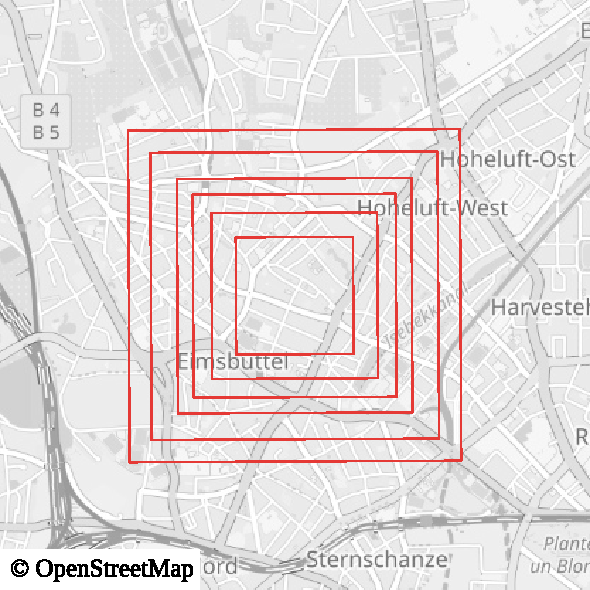
\includegraphics[width=\textwidth]{images/qgis-overview-city-rural_city}
					\end{figcenter}
				\end{minipage}
				\hspace{0.04\textwidth}
				\begin{minipage}[t]{.38\textwidth}
					\begin{figcenter}
						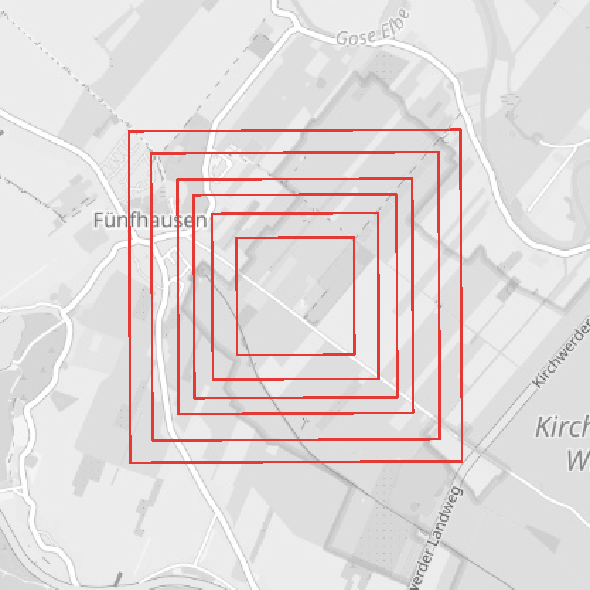
\includegraphics[width=\textwidth]{images/qgis-overview-city-rural_rural}
					\end{figcenter}
				\end{minipage}
				\caption{All six regions from 0.5km\textsuperscript{2} to 4km\textsuperscript{2} of the \enquote{OSM city} datasets (left) and \enquote{OSM rural} datasets (right).}
			\end{figure}
		
		\subsubsection{Optimizations}
		
			As described in \Cref{chap:implementation}, there were several optimizations made to the implementation.
			Some of which are on the level of data structures, some on algorithmic level.
			The effectiveness of these optimization was also evaluated using the OSM dataset.
			Each of the following optimizations was deactivated or replaced for the evaluation:

			\begin{description}
				\item[Shadow areas] Instead, every visibility check was performed using the custom intersection check described in \Cref{subsubsec:intersection-checks}.
				\item[Custom intersection check] The custom intersection check was replaced by the \texttt{RobustLineIntersector} class from the NTS to determine intersections between line segments.
				\item[BinIndex] Instead, the \texttt{Bintree} from the NTS was used.
				\item[Convex hull] The restriction to only consider vertices on the convex hull of obstacles was removed.
				\item[Valid angle areas] Considering only potential visibility neighbors within certain angular ranges was deactivated.
				\item[$k$-NN search] The $k$ of the k-NN search was deactivated to determine all visibility neighbors in all directions.
			\end{description}		
			
		\subsubsection{Measurement method}
		
			Measuring the performance was done by a small agent-based simulation project called \texttt{HikerModel}, which consists of one agent, a list of coordinates and the input dataset.
			The coordinates are given via a linestring within a GeoJSON file and each coordinate in this linestring is visited by the agent using the hybrid routing algorithm to determine the path from one location the the next.
%			The time of the graph generation as well as the time of each routing request are measured.
			Each waypoint was within the range of the dataset, meaning each coordinate was surrounded by obstacles.
			The euclidean distances (beeline distances) of the line segments within this linestring were distributed evenly to measure the required routing time relative to the distance and dataset size.
			
			Because the OSM datasets within one category cover differently sized areas, each waypoint linestring of a dataset contains all waypoints of the next smaller one plus some additional ones.
			This the waypoints of the smallest dataset are used by every other dataset as well.
%			In other words, the second smallest dataset contains all waypoints of the smallest plus some additional ones.
%			The third smallest contains all waypoints of the second smallest plus some additional ones, and so on.
		
		\subsubsection{Technical considerations}
		
			The measurement was done by a helper class \texttt{PerformanceMeasurement} providing a method accepting a function delegate which execution time is then measured.
			
			As part of its memory management, C\#/.NET uses automatic garbage collection adding unavoidable noise to the measurements.
			Unfortunately the garbage collector cannot be turned off and controling it is only partially possible.
		
			C\#/.NET also uses just-in-time (JIT) compilation changing the code during runtime.
			This can also not be turned off for normal .NET executions via the command \texttt{dotnet program.dll}.
			An alternative would be the usage of ahead-of-time (AOT) compilation, which has a negative impact on the performance of LINQ operations\footnote{According to \url{https://learn.microsoft.com/en-us/dotnet/core/deploying/native-aot/?tabs=net7}}, which in turn are used very often in the implementation.
			Because both compilation strategies have disadvantages, the normal .NET-based execution was chosen, even though it contains JIT compilation.
			
			To mitigate this dynamic behavior and to generally get resilient results, the import and each routing request was performes multiple times.
			Precisely, three warm-up iterations were performed before measuring the times of five actual execution iterations.
			The execution times from the warm-up iterations indicated that three warm-up iterations were enough for the runtime to perform the JIT compilation and prepare the garbage collector.
			
			Additionally, the garbage collector was triggered during each of the eight iterations just before calling the measured function with the goal to provide equal circumstances to all iterations.
			This was done by the \texttt{GC.Collect()} and \texttt{GC.WaitForPendingFinalizers()} methods from the \texttt{GC} class of the .NET framework.
			Using these two methods forces a garbage collection and waits for it to finish\cite{ms-gc}.
			
			To prevent the garbage collection from interfering with the execution, a 256 MiB large no-GC-region is placed around the function call via \texttt{GC.TryStartNoGCRegion(256 * 1024 * 1024)}.
			This only works if enough memory is available\cite{ms-no-gc-region}, which was the case, and introducing this no-GC-region reduced the variance of the measured times.
			\todo[inline]{\enquote{reduced the variance of the measured times} \textrightarrow\ measure/test this?}
			
			Another step to get stable and reproducable results was the increase of the process priority.
			This aims to the exclusive use of one CPU core on which this single threaded application ran.
			Increasing the process priority was done by settings the \texttt{PriorityClass} property of the current process to \texttt{ProcessPriorityClass.High}, which required root permissions on Linux systems.
		
		\subsubsection{System and hardware}
		
			The measurements were performed on an up-to-date Arch Linux operating system (Kernel 6.4.3) with .NET Core 7.0.107 and MARS framework 4.5.2.
			Apart from necessary operating system processes and the simple desktop environment i3, no other applications ran during the performance measurements.
			
			The hardware consisted of an octa core Intel\textregistered\ Xeon\textregistered\ E3-1231 v3 CPU at 3.40 GHz, a total of 16GB DDR3 1333 MHz RAM and a Samsung EVO 850 SSD.
			However, the whole algorithm and the \texttt{HikerModel} simulation is single threaded.
			File system operations are only performed to initially load the input data and to write the results after performaing all measurements.
	
\section{Performance evaluation}

	In this section the results of the performance evaluation of the algorithm are presented.
	First the OSM-based datasets are discussed followed by the artificial pattern-based datasets.

	\subsection{OSM-based datasets}
		
		\subsubsection{Import and graph generation}
		
			A few aspects regarding the runtime behavior can be inferred from the general graph generation times shown in \Cref{fig:eval-import-city} and \Cref{fig:eval-import-rural}.
			
			\begin{figure}[h!]
				\begin{minipage}{.48\textwidth}
					\begin{subfigure}[t]{\linewidth}
						\begin{figcenter}
							\begingroup%
\makeatletter%
\begin{pgfpicture}%
\pgfpathrectangle{\pgfpointorigin}{\pgfqpoint{3.041406in}{1.869661in}}%
\pgfusepath{use as bounding box}%
\begin{pgfscope}%
\pgfsetbuttcap%
\pgfsetmiterjoin%
\definecolor{currentfill}{rgb}{1.000000,1.000000,1.000000}%
\pgfsetfillcolor{currentfill}%
\pgfsetlinewidth{0.000000pt}%
\definecolor{currentstroke}{rgb}{1.000000,1.000000,1.000000}%
\pgfsetstrokecolor{currentstroke}%
\pgfsetdash{}{0pt}%
\pgfpathmoveto{\pgfqpoint{0.000000in}{0.000000in}}%
\pgfpathlineto{\pgfqpoint{3.041406in}{0.000000in}}%
\pgfpathlineto{\pgfqpoint{3.041406in}{1.869661in}}%
\pgfpathlineto{\pgfqpoint{0.000000in}{1.869661in}}%
\pgfpathlineto{\pgfqpoint{0.000000in}{0.000000in}}%
\pgfpathclose%
\pgfusepath{fill}%
\end{pgfscope}%
\begin{pgfscope}%
\pgfsetbuttcap%
\pgfsetmiterjoin%
\definecolor{currentfill}{rgb}{1.000000,1.000000,1.000000}%
\pgfsetfillcolor{currentfill}%
\pgfsetlinewidth{0.000000pt}%
\definecolor{currentstroke}{rgb}{0.000000,0.000000,0.000000}%
\pgfsetstrokecolor{currentstroke}%
\pgfsetstrokeopacity{0.000000}%
\pgfsetdash{}{0pt}%
\pgfpathmoveto{\pgfqpoint{0.601779in}{0.451389in}}%
\pgfpathlineto{\pgfqpoint{3.041406in}{0.451389in}}%
\pgfpathlineto{\pgfqpoint{3.041406in}{1.848071in}}%
\pgfpathlineto{\pgfqpoint{0.601779in}{1.848071in}}%
\pgfpathlineto{\pgfqpoint{0.601779in}{0.451389in}}%
\pgfpathclose%
\pgfusepath{fill}%
\end{pgfscope}%
\begin{pgfscope}%
\pgfpathrectangle{\pgfqpoint{0.601779in}{0.451389in}}{\pgfqpoint{2.439626in}{1.396682in}}%
\pgfusepath{clip}%
\pgfsetroundcap%
\pgfsetroundjoin%
\pgfsetlinewidth{1.003750pt}%
\definecolor{currentstroke}{rgb}{0.800000,0.800000,0.800000}%
\pgfsetstrokecolor{currentstroke}%
\pgfsetdash{}{0pt}%
\pgfpathmoveto{\pgfqpoint{0.601779in}{0.451389in}}%
\pgfpathlineto{\pgfqpoint{0.601779in}{1.848071in}}%
\pgfusepath{stroke}%
\end{pgfscope}%
\begin{pgfscope}%
\definecolor{textcolor}{rgb}{0.150000,0.150000,0.150000}%
\pgfsetstrokecolor{textcolor}%
\pgfsetfillcolor{textcolor}%
\pgftext[x=0.601779in,y=0.319444in,,top]{\color{textcolor}\sffamily\fontsize{9.000000}{10.800000}\selectfont 0}%
\end{pgfscope}%
\begin{pgfscope}%
\pgfpathrectangle{\pgfqpoint{0.601779in}{0.451389in}}{\pgfqpoint{2.439626in}{1.396682in}}%
\pgfusepath{clip}%
\pgfsetroundcap%
\pgfsetroundjoin%
\pgfsetlinewidth{1.003750pt}%
\definecolor{currentstroke}{rgb}{0.800000,0.800000,0.800000}%
\pgfsetstrokecolor{currentstroke}%
\pgfsetdash{}{0pt}%
\pgfpathmoveto{\pgfqpoint{1.121799in}{0.451389in}}%
\pgfpathlineto{\pgfqpoint{1.121799in}{1.848071in}}%
\pgfusepath{stroke}%
\end{pgfscope}%
\begin{pgfscope}%
\definecolor{textcolor}{rgb}{0.150000,0.150000,0.150000}%
\pgfsetstrokecolor{textcolor}%
\pgfsetfillcolor{textcolor}%
\pgftext[x=1.121799in,y=0.319444in,,top]{\color{textcolor}\sffamily\fontsize{9.000000}{10.800000}\selectfont 10000}%
\end{pgfscope}%
\begin{pgfscope}%
\pgfpathrectangle{\pgfqpoint{0.601779in}{0.451389in}}{\pgfqpoint{2.439626in}{1.396682in}}%
\pgfusepath{clip}%
\pgfsetroundcap%
\pgfsetroundjoin%
\pgfsetlinewidth{1.003750pt}%
\definecolor{currentstroke}{rgb}{0.800000,0.800000,0.800000}%
\pgfsetstrokecolor{currentstroke}%
\pgfsetdash{}{0pt}%
\pgfpathmoveto{\pgfqpoint{1.641819in}{0.451389in}}%
\pgfpathlineto{\pgfqpoint{1.641819in}{1.848071in}}%
\pgfusepath{stroke}%
\end{pgfscope}%
\begin{pgfscope}%
\definecolor{textcolor}{rgb}{0.150000,0.150000,0.150000}%
\pgfsetstrokecolor{textcolor}%
\pgfsetfillcolor{textcolor}%
\pgftext[x=1.641819in,y=0.319444in,,top]{\color{textcolor}\sffamily\fontsize{9.000000}{10.800000}\selectfont 20000}%
\end{pgfscope}%
\begin{pgfscope}%
\pgfpathrectangle{\pgfqpoint{0.601779in}{0.451389in}}{\pgfqpoint{2.439626in}{1.396682in}}%
\pgfusepath{clip}%
\pgfsetroundcap%
\pgfsetroundjoin%
\pgfsetlinewidth{1.003750pt}%
\definecolor{currentstroke}{rgb}{0.800000,0.800000,0.800000}%
\pgfsetstrokecolor{currentstroke}%
\pgfsetdash{}{0pt}%
\pgfpathmoveto{\pgfqpoint{2.161839in}{0.451389in}}%
\pgfpathlineto{\pgfqpoint{2.161839in}{1.848071in}}%
\pgfusepath{stroke}%
\end{pgfscope}%
\begin{pgfscope}%
\definecolor{textcolor}{rgb}{0.150000,0.150000,0.150000}%
\pgfsetstrokecolor{textcolor}%
\pgfsetfillcolor{textcolor}%
\pgftext[x=2.161839in,y=0.319444in,,top]{\color{textcolor}\sffamily\fontsize{9.000000}{10.800000}\selectfont 30000}%
\end{pgfscope}%
\begin{pgfscope}%
\pgfpathrectangle{\pgfqpoint{0.601779in}{0.451389in}}{\pgfqpoint{2.439626in}{1.396682in}}%
\pgfusepath{clip}%
\pgfsetroundcap%
\pgfsetroundjoin%
\pgfsetlinewidth{1.003750pt}%
\definecolor{currentstroke}{rgb}{0.800000,0.800000,0.800000}%
\pgfsetstrokecolor{currentstroke}%
\pgfsetdash{}{0pt}%
\pgfpathmoveto{\pgfqpoint{2.681859in}{0.451389in}}%
\pgfpathlineto{\pgfqpoint{2.681859in}{1.848071in}}%
\pgfusepath{stroke}%
\end{pgfscope}%
\begin{pgfscope}%
\definecolor{textcolor}{rgb}{0.150000,0.150000,0.150000}%
\pgfsetstrokecolor{textcolor}%
\pgfsetfillcolor{textcolor}%
\pgftext[x=2.681859in,y=0.319444in,,top]{\color{textcolor}\sffamily\fontsize{9.000000}{10.800000}\selectfont 40000}%
\end{pgfscope}%
\begin{pgfscope}%
\definecolor{textcolor}{rgb}{0.150000,0.150000,0.150000}%
\pgfsetstrokecolor{textcolor}%
\pgfsetfillcolor{textcolor}%
\pgftext[x=1.821593in,y=0.125000in,,top]{\color{textcolor}\sffamily\fontsize{9.000000}{10.800000}\selectfont Input obstacle vertices}%
\end{pgfscope}%
\begin{pgfscope}%
\pgfpathrectangle{\pgfqpoint{0.601779in}{0.451389in}}{\pgfqpoint{2.439626in}{1.396682in}}%
\pgfusepath{clip}%
\pgfsetroundcap%
\pgfsetroundjoin%
\pgfsetlinewidth{1.003750pt}%
\definecolor{currentstroke}{rgb}{0.800000,0.800000,0.800000}%
\pgfsetstrokecolor{currentstroke}%
\pgfsetdash{}{0pt}%
\pgfpathmoveto{\pgfqpoint{0.601779in}{0.451389in}}%
\pgfpathlineto{\pgfqpoint{3.041406in}{0.451389in}}%
\pgfusepath{stroke}%
\end{pgfscope}%
\begin{pgfscope}%
\definecolor{textcolor}{rgb}{0.150000,0.150000,0.150000}%
\pgfsetstrokecolor{textcolor}%
\pgfsetfillcolor{textcolor}%
\pgftext[x=0.400987in, y=0.403903in, left, base]{\color{textcolor}\sffamily\fontsize{9.000000}{10.800000}\selectfont 0}%
\end{pgfscope}%
\begin{pgfscope}%
\pgfpathrectangle{\pgfqpoint{0.601779in}{0.451389in}}{\pgfqpoint{2.439626in}{1.396682in}}%
\pgfusepath{clip}%
\pgfsetroundcap%
\pgfsetroundjoin%
\pgfsetlinewidth{1.003750pt}%
\definecolor{currentstroke}{rgb}{0.800000,0.800000,0.800000}%
\pgfsetstrokecolor{currentstroke}%
\pgfsetdash{}{0pt}%
\pgfpathmoveto{\pgfqpoint{0.601779in}{0.794085in}}%
\pgfpathlineto{\pgfqpoint{3.041406in}{0.794085in}}%
\pgfusepath{stroke}%
\end{pgfscope}%
\begin{pgfscope}%
\definecolor{textcolor}{rgb}{0.150000,0.150000,0.150000}%
\pgfsetstrokecolor{textcolor}%
\pgfsetfillcolor{textcolor}%
\pgftext[x=0.263292in, y=0.746600in, left, base]{\color{textcolor}\sffamily\fontsize{9.000000}{10.800000}\selectfont 250}%
\end{pgfscope}%
\begin{pgfscope}%
\pgfpathrectangle{\pgfqpoint{0.601779in}{0.451389in}}{\pgfqpoint{2.439626in}{1.396682in}}%
\pgfusepath{clip}%
\pgfsetroundcap%
\pgfsetroundjoin%
\pgfsetlinewidth{1.003750pt}%
\definecolor{currentstroke}{rgb}{0.800000,0.800000,0.800000}%
\pgfsetstrokecolor{currentstroke}%
\pgfsetdash{}{0pt}%
\pgfpathmoveto{\pgfqpoint{0.601779in}{1.136782in}}%
\pgfpathlineto{\pgfqpoint{3.041406in}{1.136782in}}%
\pgfusepath{stroke}%
\end{pgfscope}%
\begin{pgfscope}%
\definecolor{textcolor}{rgb}{0.150000,0.150000,0.150000}%
\pgfsetstrokecolor{textcolor}%
\pgfsetfillcolor{textcolor}%
\pgftext[x=0.263292in, y=1.089297in, left, base]{\color{textcolor}\sffamily\fontsize{9.000000}{10.800000}\selectfont 500}%
\end{pgfscope}%
\begin{pgfscope}%
\pgfpathrectangle{\pgfqpoint{0.601779in}{0.451389in}}{\pgfqpoint{2.439626in}{1.396682in}}%
\pgfusepath{clip}%
\pgfsetroundcap%
\pgfsetroundjoin%
\pgfsetlinewidth{1.003750pt}%
\definecolor{currentstroke}{rgb}{0.800000,0.800000,0.800000}%
\pgfsetstrokecolor{currentstroke}%
\pgfsetdash{}{0pt}%
\pgfpathmoveto{\pgfqpoint{0.601779in}{1.479479in}}%
\pgfpathlineto{\pgfqpoint{3.041406in}{1.479479in}}%
\pgfusepath{stroke}%
\end{pgfscope}%
\begin{pgfscope}%
\definecolor{textcolor}{rgb}{0.150000,0.150000,0.150000}%
\pgfsetstrokecolor{textcolor}%
\pgfsetfillcolor{textcolor}%
\pgftext[x=0.263292in, y=1.431993in, left, base]{\color{textcolor}\sffamily\fontsize{9.000000}{10.800000}\selectfont 750}%
\end{pgfscope}%
\begin{pgfscope}%
\pgfpathrectangle{\pgfqpoint{0.601779in}{0.451389in}}{\pgfqpoint{2.439626in}{1.396682in}}%
\pgfusepath{clip}%
\pgfsetroundcap%
\pgfsetroundjoin%
\pgfsetlinewidth{1.003750pt}%
\definecolor{currentstroke}{rgb}{0.800000,0.800000,0.800000}%
\pgfsetstrokecolor{currentstroke}%
\pgfsetdash{}{0pt}%
\pgfpathmoveto{\pgfqpoint{0.601779in}{1.822175in}}%
\pgfpathlineto{\pgfqpoint{3.041406in}{1.822175in}}%
\pgfusepath{stroke}%
\end{pgfscope}%
\begin{pgfscope}%
\definecolor{textcolor}{rgb}{0.150000,0.150000,0.150000}%
\pgfsetstrokecolor{textcolor}%
\pgfsetfillcolor{textcolor}%
\pgftext[x=0.194444in, y=1.774690in, left, base]{\color{textcolor}\sffamily\fontsize{9.000000}{10.800000}\selectfont 1000}%
\end{pgfscope}%
\begin{pgfscope}%
\definecolor{textcolor}{rgb}{0.150000,0.150000,0.150000}%
\pgfsetstrokecolor{textcolor}%
\pgfsetfillcolor{textcolor}%
\pgftext[x=0.125000in,y=1.149730in,,bottom,rotate=90.000000]{\color{textcolor}\sffamily\fontsize{9.000000}{10.800000}\selectfont Time in s}%
\end{pgfscope}%
\begin{pgfscope}%
\pgfpathrectangle{\pgfqpoint{0.601779in}{0.451389in}}{\pgfqpoint{2.439626in}{1.396682in}}%
\pgfusepath{clip}%
\pgfsetbuttcap%
\pgfsetroundjoin%
\definecolor{currentfill}{rgb}{0.003922,0.450980,0.698039}%
\pgfsetfillcolor{currentfill}%
\pgfsetfillopacity{0.200000}%
\pgfsetlinewidth{1.003750pt}%
\definecolor{currentstroke}{rgb}{0.003922,0.450980,0.698039}%
\pgfsetstrokecolor{currentstroke}%
\pgfsetstrokeopacity{0.200000}%
\pgfsetdash{}{0pt}%
\pgfsys@defobject{currentmarker}{\pgfqpoint{0.970786in}{0.475103in}}{\pgfqpoint{2.942805in}{1.782692in}}{%
\pgfpathmoveto{\pgfqpoint{0.970786in}{0.475365in}}%
\pgfpathlineto{\pgfqpoint{0.970786in}{0.475103in}}%
\pgfpathlineto{\pgfqpoint{1.270421in}{0.525314in}}%
\pgfpathlineto{\pgfqpoint{1.532303in}{0.609750in}}%
\pgfpathlineto{\pgfqpoint{1.787477in}{0.734608in}}%
\pgfpathlineto{\pgfqpoint{2.380975in}{1.150136in}}%
\pgfpathlineto{\pgfqpoint{2.942805in}{1.763790in}}%
\pgfpathlineto{\pgfqpoint{2.942805in}{1.782692in}}%
\pgfpathlineto{\pgfqpoint{2.942805in}{1.782692in}}%
\pgfpathlineto{\pgfqpoint{2.380975in}{1.159429in}}%
\pgfpathlineto{\pgfqpoint{1.787477in}{0.735896in}}%
\pgfpathlineto{\pgfqpoint{1.532303in}{0.612478in}}%
\pgfpathlineto{\pgfqpoint{1.270421in}{0.526536in}}%
\pgfpathlineto{\pgfqpoint{0.970786in}{0.475365in}}%
\pgfpathlineto{\pgfqpoint{0.970786in}{0.475365in}}%
\pgfpathclose%
\pgfusepath{stroke,fill}%
}%
\begin{pgfscope}%
\pgfsys@transformshift{0.000000in}{0.000000in}%
\pgfsys@useobject{currentmarker}{}%
\end{pgfscope}%
\end{pgfscope}%
\begin{pgfscope}%
\pgfsetrectcap%
\pgfsetmiterjoin%
\pgfsetlinewidth{1.254687pt}%
\definecolor{currentstroke}{rgb}{0.800000,0.800000,0.800000}%
\pgfsetstrokecolor{currentstroke}%
\pgfsetdash{}{0pt}%
\pgfpathmoveto{\pgfqpoint{0.601779in}{0.451389in}}%
\pgfpathlineto{\pgfqpoint{0.601779in}{1.848071in}}%
\pgfusepath{stroke}%
\end{pgfscope}%
\begin{pgfscope}%
\pgfsetrectcap%
\pgfsetmiterjoin%
\pgfsetlinewidth{1.254687pt}%
\definecolor{currentstroke}{rgb}{0.800000,0.800000,0.800000}%
\pgfsetstrokecolor{currentstroke}%
\pgfsetdash{}{0pt}%
\pgfpathmoveto{\pgfqpoint{3.041406in}{0.451389in}}%
\pgfpathlineto{\pgfqpoint{3.041406in}{1.848071in}}%
\pgfusepath{stroke}%
\end{pgfscope}%
\begin{pgfscope}%
\pgfsetrectcap%
\pgfsetmiterjoin%
\pgfsetlinewidth{1.254687pt}%
\definecolor{currentstroke}{rgb}{0.800000,0.800000,0.800000}%
\pgfsetstrokecolor{currentstroke}%
\pgfsetdash{}{0pt}%
\pgfpathmoveto{\pgfqpoint{0.601779in}{0.451389in}}%
\pgfpathlineto{\pgfqpoint{3.041406in}{0.451389in}}%
\pgfusepath{stroke}%
\end{pgfscope}%
\begin{pgfscope}%
\pgfsetrectcap%
\pgfsetmiterjoin%
\pgfsetlinewidth{1.254687pt}%
\definecolor{currentstroke}{rgb}{0.800000,0.800000,0.800000}%
\pgfsetstrokecolor{currentstroke}%
\pgfsetdash{}{0pt}%
\pgfpathmoveto{\pgfqpoint{0.601779in}{1.848071in}}%
\pgfpathlineto{\pgfqpoint{3.041406in}{1.848071in}}%
\pgfusepath{stroke}%
\end{pgfscope}%
\begin{pgfscope}%
\pgfsetroundcap%
\pgfsetroundjoin%
\pgfsetlinewidth{1.003750pt}%
\definecolor{currentstroke}{rgb}{0.003922,0.450980,0.698039}%
\pgfsetstrokecolor{currentstroke}%
\pgfsetdash{}{0pt}%
\pgfpathmoveto{\pgfqpoint{0.970786in}{0.475218in}}%
\pgfpathlineto{\pgfqpoint{1.270421in}{0.525877in}}%
\pgfpathlineto{\pgfqpoint{1.532303in}{0.611282in}}%
\pgfpathlineto{\pgfqpoint{1.787477in}{0.735321in}}%
\pgfpathlineto{\pgfqpoint{2.380975in}{1.154498in}}%
\pgfpathlineto{\pgfqpoint{2.942805in}{1.771598in}}%
\pgfusepath{stroke}%
\end{pgfscope}%
\begin{pgfscope}%
\pgfsetbuttcap%
\pgfsetroundjoin%
\definecolor{currentfill}{rgb}{0.003922,0.450980,0.698039}%
\pgfsetfillcolor{currentfill}%
\pgfsetlinewidth{0.752812pt}%
\definecolor{currentstroke}{rgb}{1.000000,1.000000,1.000000}%
\pgfsetstrokecolor{currentstroke}%
\pgfsetdash{}{0pt}%
\pgfsys@defobject{currentmarker}{\pgfqpoint{-0.034722in}{-0.034722in}}{\pgfqpoint{0.034722in}{0.034722in}}{%
\pgfpathmoveto{\pgfqpoint{0.000000in}{-0.034722in}}%
\pgfpathcurveto{\pgfqpoint{0.009208in}{-0.034722in}}{\pgfqpoint{0.018041in}{-0.031064in}}{\pgfqpoint{0.024552in}{-0.024552in}}%
\pgfpathcurveto{\pgfqpoint{0.031064in}{-0.018041in}}{\pgfqpoint{0.034722in}{-0.009208in}}{\pgfqpoint{0.034722in}{0.000000in}}%
\pgfpathcurveto{\pgfqpoint{0.034722in}{0.009208in}}{\pgfqpoint{0.031064in}{0.018041in}}{\pgfqpoint{0.024552in}{0.024552in}}%
\pgfpathcurveto{\pgfqpoint{0.018041in}{0.031064in}}{\pgfqpoint{0.009208in}{0.034722in}}{\pgfqpoint{0.000000in}{0.034722in}}%
\pgfpathcurveto{\pgfqpoint{-0.009208in}{0.034722in}}{\pgfqpoint{-0.018041in}{0.031064in}}{\pgfqpoint{-0.024552in}{0.024552in}}%
\pgfpathcurveto{\pgfqpoint{-0.031064in}{0.018041in}}{\pgfqpoint{-0.034722in}{0.009208in}}{\pgfqpoint{-0.034722in}{0.000000in}}%
\pgfpathcurveto{\pgfqpoint{-0.034722in}{-0.009208in}}{\pgfqpoint{-0.031064in}{-0.018041in}}{\pgfqpoint{-0.024552in}{-0.024552in}}%
\pgfpathcurveto{\pgfqpoint{-0.018041in}{-0.031064in}}{\pgfqpoint{-0.009208in}{-0.034722in}}{\pgfqpoint{0.000000in}{-0.034722in}}%
\pgfpathlineto{\pgfqpoint{0.000000in}{-0.034722in}}%
\pgfpathclose%
\pgfusepath{stroke,fill}%
}%
\begin{pgfscope}%
\pgfsys@transformshift{0.970786in}{0.475218in}%
\pgfsys@useobject{currentmarker}{}%
\end{pgfscope}%
\begin{pgfscope}%
\pgfsys@transformshift{1.270421in}{0.525877in}%
\pgfsys@useobject{currentmarker}{}%
\end{pgfscope}%
\begin{pgfscope}%
\pgfsys@transformshift{1.532303in}{0.611282in}%
\pgfsys@useobject{currentmarker}{}%
\end{pgfscope}%
\begin{pgfscope}%
\pgfsys@transformshift{1.787477in}{0.735321in}%
\pgfsys@useobject{currentmarker}{}%
\end{pgfscope}%
\begin{pgfscope}%
\pgfsys@transformshift{2.380975in}{1.154498in}%
\pgfsys@useobject{currentmarker}{}%
\end{pgfscope}%
\begin{pgfscope}%
\pgfsys@transformshift{2.942805in}{1.771598in}%
\pgfsys@useobject{currentmarker}{}%
\end{pgfscope}%
\end{pgfscope}%
\end{pgfpicture}%
\makeatother%
\endgroup%

						\end{figcenter}
						\caption{Total graph generation times.}
						\label{fig:eval-import-city-abs}
					\end{subfigure}
					\\[3ex]
					\begin{subfigure}[t]{\linewidth}
						\begin{figcenter}
							\begingroup%
\makeatletter%
\begin{pgfpicture}%
\pgfpathrectangle{\pgfpointorigin}{\pgfqpoint{3.043196in}{1.867995in}}%
\pgfusepath{use as bounding box}%
\begin{pgfscope}%
\pgfsetbuttcap%
\pgfsetmiterjoin%
\definecolor{currentfill}{rgb}{1.000000,1.000000,1.000000}%
\pgfsetfillcolor{currentfill}%
\pgfsetlinewidth{0.000000pt}%
\definecolor{currentstroke}{rgb}{1.000000,1.000000,1.000000}%
\pgfsetstrokecolor{currentstroke}%
\pgfsetdash{}{0pt}%
\pgfpathmoveto{\pgfqpoint{0.000000in}{0.000000in}}%
\pgfpathlineto{\pgfqpoint{3.043196in}{0.000000in}}%
\pgfpathlineto{\pgfqpoint{3.043196in}{1.867995in}}%
\pgfpathlineto{\pgfqpoint{0.000000in}{1.867995in}}%
\pgfpathlineto{\pgfqpoint{0.000000in}{0.000000in}}%
\pgfpathclose%
\pgfusepath{fill}%
\end{pgfscope}%
\begin{pgfscope}%
\pgfsetbuttcap%
\pgfsetmiterjoin%
\definecolor{currentfill}{rgb}{1.000000,1.000000,1.000000}%
\pgfsetfillcolor{currentfill}%
\pgfsetlinewidth{0.000000pt}%
\definecolor{currentstroke}{rgb}{0.000000,0.000000,0.000000}%
\pgfsetstrokecolor{currentstroke}%
\pgfsetstrokeopacity{0.000000}%
\pgfsetdash{}{0pt}%
\pgfpathmoveto{\pgfqpoint{0.395236in}{0.451389in}}%
\pgfpathlineto{\pgfqpoint{3.043196in}{0.451389in}}%
\pgfpathlineto{\pgfqpoint{3.043196in}{1.867995in}}%
\pgfpathlineto{\pgfqpoint{0.395236in}{1.867995in}}%
\pgfpathlineto{\pgfqpoint{0.395236in}{0.451389in}}%
\pgfpathclose%
\pgfusepath{fill}%
\end{pgfscope}%
\begin{pgfscope}%
\pgfpathrectangle{\pgfqpoint{0.395236in}{0.451389in}}{\pgfqpoint{2.647959in}{1.416606in}}%
\pgfusepath{clip}%
\pgfsetroundcap%
\pgfsetroundjoin%
\pgfsetlinewidth{1.003750pt}%
\definecolor{currentstroke}{rgb}{0.800000,0.800000,0.800000}%
\pgfsetstrokecolor{currentstroke}%
\pgfsetdash{}{0pt}%
\pgfpathmoveto{\pgfqpoint{0.395236in}{0.451389in}}%
\pgfpathlineto{\pgfqpoint{0.395236in}{1.867995in}}%
\pgfusepath{stroke}%
\end{pgfscope}%
\begin{pgfscope}%
\definecolor{textcolor}{rgb}{0.150000,0.150000,0.150000}%
\pgfsetstrokecolor{textcolor}%
\pgfsetfillcolor{textcolor}%
\pgftext[x=0.395236in,y=0.319444in,,top]{\color{textcolor}\sffamily\fontsize{9.000000}{10.800000}\selectfont 0}%
\end{pgfscope}%
\begin{pgfscope}%
\pgfpathrectangle{\pgfqpoint{0.395236in}{0.451389in}}{\pgfqpoint{2.647959in}{1.416606in}}%
\pgfusepath{clip}%
\pgfsetroundcap%
\pgfsetroundjoin%
\pgfsetlinewidth{1.003750pt}%
\definecolor{currentstroke}{rgb}{0.800000,0.800000,0.800000}%
\pgfsetstrokecolor{currentstroke}%
\pgfsetdash{}{0pt}%
\pgfpathmoveto{\pgfqpoint{0.800662in}{0.451389in}}%
\pgfpathlineto{\pgfqpoint{0.800662in}{1.867995in}}%
\pgfusepath{stroke}%
\end{pgfscope}%
\begin{pgfscope}%
\definecolor{textcolor}{rgb}{0.150000,0.150000,0.150000}%
\pgfsetstrokecolor{textcolor}%
\pgfsetfillcolor{textcolor}%
\pgftext[x=0.800662in,y=0.319444in,,top]{\color{textcolor}\sffamily\fontsize{9.000000}{10.800000}\selectfont 5000}%
\end{pgfscope}%
\begin{pgfscope}%
\pgfpathrectangle{\pgfqpoint{0.395236in}{0.451389in}}{\pgfqpoint{2.647959in}{1.416606in}}%
\pgfusepath{clip}%
\pgfsetroundcap%
\pgfsetroundjoin%
\pgfsetlinewidth{1.003750pt}%
\definecolor{currentstroke}{rgb}{0.800000,0.800000,0.800000}%
\pgfsetstrokecolor{currentstroke}%
\pgfsetdash{}{0pt}%
\pgfpathmoveto{\pgfqpoint{1.206089in}{0.451389in}}%
\pgfpathlineto{\pgfqpoint{1.206089in}{1.867995in}}%
\pgfusepath{stroke}%
\end{pgfscope}%
\begin{pgfscope}%
\definecolor{textcolor}{rgb}{0.150000,0.150000,0.150000}%
\pgfsetstrokecolor{textcolor}%
\pgfsetfillcolor{textcolor}%
\pgftext[x=1.206089in,y=0.319444in,,top]{\color{textcolor}\sffamily\fontsize{9.000000}{10.800000}\selectfont 10000}%
\end{pgfscope}%
\begin{pgfscope}%
\pgfpathrectangle{\pgfqpoint{0.395236in}{0.451389in}}{\pgfqpoint{2.647959in}{1.416606in}}%
\pgfusepath{clip}%
\pgfsetroundcap%
\pgfsetroundjoin%
\pgfsetlinewidth{1.003750pt}%
\definecolor{currentstroke}{rgb}{0.800000,0.800000,0.800000}%
\pgfsetstrokecolor{currentstroke}%
\pgfsetdash{}{0pt}%
\pgfpathmoveto{\pgfqpoint{1.611515in}{0.451389in}}%
\pgfpathlineto{\pgfqpoint{1.611515in}{1.867995in}}%
\pgfusepath{stroke}%
\end{pgfscope}%
\begin{pgfscope}%
\definecolor{textcolor}{rgb}{0.150000,0.150000,0.150000}%
\pgfsetstrokecolor{textcolor}%
\pgfsetfillcolor{textcolor}%
\pgftext[x=1.611515in,y=0.319444in,,top]{\color{textcolor}\sffamily\fontsize{9.000000}{10.800000}\selectfont 15000}%
\end{pgfscope}%
\begin{pgfscope}%
\pgfpathrectangle{\pgfqpoint{0.395236in}{0.451389in}}{\pgfqpoint{2.647959in}{1.416606in}}%
\pgfusepath{clip}%
\pgfsetroundcap%
\pgfsetroundjoin%
\pgfsetlinewidth{1.003750pt}%
\definecolor{currentstroke}{rgb}{0.800000,0.800000,0.800000}%
\pgfsetstrokecolor{currentstroke}%
\pgfsetdash{}{0pt}%
\pgfpathmoveto{\pgfqpoint{2.016941in}{0.451389in}}%
\pgfpathlineto{\pgfqpoint{2.016941in}{1.867995in}}%
\pgfusepath{stroke}%
\end{pgfscope}%
\begin{pgfscope}%
\definecolor{textcolor}{rgb}{0.150000,0.150000,0.150000}%
\pgfsetstrokecolor{textcolor}%
\pgfsetfillcolor{textcolor}%
\pgftext[x=2.016941in,y=0.319444in,,top]{\color{textcolor}\sffamily\fontsize{9.000000}{10.800000}\selectfont 20000}%
\end{pgfscope}%
\begin{pgfscope}%
\pgfpathrectangle{\pgfqpoint{0.395236in}{0.451389in}}{\pgfqpoint{2.647959in}{1.416606in}}%
\pgfusepath{clip}%
\pgfsetroundcap%
\pgfsetroundjoin%
\pgfsetlinewidth{1.003750pt}%
\definecolor{currentstroke}{rgb}{0.800000,0.800000,0.800000}%
\pgfsetstrokecolor{currentstroke}%
\pgfsetdash{}{0pt}%
\pgfpathmoveto{\pgfqpoint{2.422367in}{0.451389in}}%
\pgfpathlineto{\pgfqpoint{2.422367in}{1.867995in}}%
\pgfusepath{stroke}%
\end{pgfscope}%
\begin{pgfscope}%
\definecolor{textcolor}{rgb}{0.150000,0.150000,0.150000}%
\pgfsetstrokecolor{textcolor}%
\pgfsetfillcolor{textcolor}%
\pgftext[x=2.422367in,y=0.319444in,,top]{\color{textcolor}\sffamily\fontsize{9.000000}{10.800000}\selectfont 25000}%
\end{pgfscope}%
\begin{pgfscope}%
\pgfpathrectangle{\pgfqpoint{0.395236in}{0.451389in}}{\pgfqpoint{2.647959in}{1.416606in}}%
\pgfusepath{clip}%
\pgfsetroundcap%
\pgfsetroundjoin%
\pgfsetlinewidth{1.003750pt}%
\definecolor{currentstroke}{rgb}{0.800000,0.800000,0.800000}%
\pgfsetstrokecolor{currentstroke}%
\pgfsetdash{}{0pt}%
\pgfpathmoveto{\pgfqpoint{2.827793in}{0.451389in}}%
\pgfpathlineto{\pgfqpoint{2.827793in}{1.867995in}}%
\pgfusepath{stroke}%
\end{pgfscope}%
\begin{pgfscope}%
\definecolor{textcolor}{rgb}{0.150000,0.150000,0.150000}%
\pgfsetstrokecolor{textcolor}%
\pgfsetfillcolor{textcolor}%
\pgftext[x=2.827793in,y=0.319444in,,top]{\color{textcolor}\sffamily\fontsize{9.000000}{10.800000}\selectfont 30000}%
\end{pgfscope}%
\begin{pgfscope}%
\definecolor{textcolor}{rgb}{0.150000,0.150000,0.150000}%
\pgfsetstrokecolor{textcolor}%
\pgfsetfillcolor{textcolor}%
\pgftext[x=1.719216in,y=0.125000in,,top]{\color{textcolor}\sffamily\fontsize{9.000000}{10.800000}\selectfont Input obstacle vertices}%
\end{pgfscope}%
\begin{pgfscope}%
\pgfpathrectangle{\pgfqpoint{0.395236in}{0.451389in}}{\pgfqpoint{2.647959in}{1.416606in}}%
\pgfusepath{clip}%
\pgfsetroundcap%
\pgfsetroundjoin%
\pgfsetlinewidth{1.003750pt}%
\definecolor{currentstroke}{rgb}{0.800000,0.800000,0.800000}%
\pgfsetstrokecolor{currentstroke}%
\pgfsetdash{}{0pt}%
\pgfpathmoveto{\pgfqpoint{0.395236in}{0.451389in}}%
\pgfpathlineto{\pgfqpoint{3.043196in}{0.451389in}}%
\pgfusepath{stroke}%
\end{pgfscope}%
\begin{pgfscope}%
\definecolor{textcolor}{rgb}{0.150000,0.150000,0.150000}%
\pgfsetstrokecolor{textcolor}%
\pgfsetfillcolor{textcolor}%
\pgftext[x=0.194444in, y=0.403903in, left, base]{\color{textcolor}\sffamily\fontsize{9.000000}{10.800000}\selectfont 0}%
\end{pgfscope}%
\begin{pgfscope}%
\pgfpathrectangle{\pgfqpoint{0.395236in}{0.451389in}}{\pgfqpoint{2.647959in}{1.416606in}}%
\pgfusepath{clip}%
\pgfsetroundcap%
\pgfsetroundjoin%
\pgfsetlinewidth{1.003750pt}%
\definecolor{currentstroke}{rgb}{0.800000,0.800000,0.800000}%
\pgfsetstrokecolor{currentstroke}%
\pgfsetdash{}{0pt}%
\pgfpathmoveto{\pgfqpoint{0.395236in}{0.854358in}}%
\pgfpathlineto{\pgfqpoint{3.043196in}{0.854358in}}%
\pgfusepath{stroke}%
\end{pgfscope}%
\begin{pgfscope}%
\definecolor{textcolor}{rgb}{0.150000,0.150000,0.150000}%
\pgfsetstrokecolor{textcolor}%
\pgfsetfillcolor{textcolor}%
\pgftext[x=0.194444in, y=0.806873in, left, base]{\color{textcolor}\sffamily\fontsize{9.000000}{10.800000}\selectfont 2}%
\end{pgfscope}%
\begin{pgfscope}%
\pgfpathrectangle{\pgfqpoint{0.395236in}{0.451389in}}{\pgfqpoint{2.647959in}{1.416606in}}%
\pgfusepath{clip}%
\pgfsetroundcap%
\pgfsetroundjoin%
\pgfsetlinewidth{1.003750pt}%
\definecolor{currentstroke}{rgb}{0.800000,0.800000,0.800000}%
\pgfsetstrokecolor{currentstroke}%
\pgfsetdash{}{0pt}%
\pgfpathmoveto{\pgfqpoint{0.395236in}{1.257328in}}%
\pgfpathlineto{\pgfqpoint{3.043196in}{1.257328in}}%
\pgfusepath{stroke}%
\end{pgfscope}%
\begin{pgfscope}%
\definecolor{textcolor}{rgb}{0.150000,0.150000,0.150000}%
\pgfsetstrokecolor{textcolor}%
\pgfsetfillcolor{textcolor}%
\pgftext[x=0.194444in, y=1.209842in, left, base]{\color{textcolor}\sffamily\fontsize{9.000000}{10.800000}\selectfont 4}%
\end{pgfscope}%
\begin{pgfscope}%
\pgfpathrectangle{\pgfqpoint{0.395236in}{0.451389in}}{\pgfqpoint{2.647959in}{1.416606in}}%
\pgfusepath{clip}%
\pgfsetroundcap%
\pgfsetroundjoin%
\pgfsetlinewidth{1.003750pt}%
\definecolor{currentstroke}{rgb}{0.800000,0.800000,0.800000}%
\pgfsetstrokecolor{currentstroke}%
\pgfsetdash{}{0pt}%
\pgfpathmoveto{\pgfqpoint{0.395236in}{1.660297in}}%
\pgfpathlineto{\pgfqpoint{3.043196in}{1.660297in}}%
\pgfusepath{stroke}%
\end{pgfscope}%
\begin{pgfscope}%
\definecolor{textcolor}{rgb}{0.150000,0.150000,0.150000}%
\pgfsetstrokecolor{textcolor}%
\pgfsetfillcolor{textcolor}%
\pgftext[x=0.194444in, y=1.612812in, left, base]{\color{textcolor}\sffamily\fontsize{9.000000}{10.800000}\selectfont 6}%
\end{pgfscope}%
\begin{pgfscope}%
\definecolor{textcolor}{rgb}{0.150000,0.150000,0.150000}%
\pgfsetstrokecolor{textcolor}%
\pgfsetfillcolor{textcolor}%
\pgftext[x=0.125000in,y=1.159692in,,bottom,rotate=90.000000]{\color{textcolor}\sffamily\fontsize{9.000000}{10.800000}\selectfont Time in ms}%
\end{pgfscope}%
\begin{pgfscope}%
\pgfpathrectangle{\pgfqpoint{0.395236in}{0.451389in}}{\pgfqpoint{2.647959in}{1.416606in}}%
\pgfusepath{clip}%
\pgfsetbuttcap%
\pgfsetroundjoin%
\definecolor{currentfill}{rgb}{0.003922,0.450980,0.698039}%
\pgfsetfillcolor{currentfill}%
\pgfsetfillopacity{0.200000}%
\pgfsetlinewidth{1.003750pt}%
\definecolor{currentstroke}{rgb}{0.003922,0.450980,0.698039}%
\pgfsetstrokecolor{currentstroke}%
\pgfsetstrokeopacity{0.200000}%
\pgfsetdash{}{0pt}%
\pgfsys@defobject{currentmarker}{\pgfqpoint{0.399615in}{0.472653in}}{\pgfqpoint{2.917311in}{1.801550in}}{%
\pgfpathmoveto{\pgfqpoint{0.399615in}{0.483482in}}%
\pgfpathlineto{\pgfqpoint{0.399615in}{0.472653in}}%
\pgfpathlineto{\pgfqpoint{0.412751in}{0.490586in}}%
\pgfpathlineto{\pgfqpoint{0.465294in}{0.494104in}}%
\pgfpathlineto{\pgfqpoint{0.552866in}{0.542933in}}%
\pgfpathlineto{\pgfqpoint{0.675467in}{0.592283in}}%
\pgfpathlineto{\pgfqpoint{0.833097in}{0.656559in}}%
\pgfpathlineto{\pgfqpoint{1.025755in}{0.752049in}}%
\pgfpathlineto{\pgfqpoint{1.253442in}{0.853539in}}%
\pgfpathlineto{\pgfqpoint{1.516158in}{0.976622in}}%
\pgfpathlineto{\pgfqpoint{1.813903in}{1.168476in}}%
\pgfpathlineto{\pgfqpoint{2.146677in}{1.309545in}}%
\pgfpathlineto{\pgfqpoint{2.514480in}{1.529714in}}%
\pgfpathlineto{\pgfqpoint{2.917311in}{1.794932in}}%
\pgfpathlineto{\pgfqpoint{2.917311in}{1.801550in}}%
\pgfpathlineto{\pgfqpoint{2.917311in}{1.801550in}}%
\pgfpathlineto{\pgfqpoint{2.514480in}{1.535942in}}%
\pgfpathlineto{\pgfqpoint{2.146677in}{1.320504in}}%
\pgfpathlineto{\pgfqpoint{1.813903in}{1.179577in}}%
\pgfpathlineto{\pgfqpoint{1.516158in}{0.980885in}}%
\pgfpathlineto{\pgfqpoint{1.253442in}{0.857408in}}%
\pgfpathlineto{\pgfqpoint{1.025755in}{0.753562in}}%
\pgfpathlineto{\pgfqpoint{0.833097in}{0.657935in}}%
\pgfpathlineto{\pgfqpoint{0.675467in}{0.592683in}}%
\pgfpathlineto{\pgfqpoint{0.552866in}{0.543553in}}%
\pgfpathlineto{\pgfqpoint{0.465294in}{0.495044in}}%
\pgfpathlineto{\pgfqpoint{0.412751in}{0.494366in}}%
\pgfpathlineto{\pgfqpoint{0.399615in}{0.483482in}}%
\pgfpathlineto{\pgfqpoint{0.399615in}{0.483482in}}%
\pgfpathclose%
\pgfusepath{stroke,fill}%
}%
\begin{pgfscope}%
\pgfsys@transformshift{0.000000in}{0.000000in}%
\pgfsys@useobject{currentmarker}{}%
\end{pgfscope}%
\end{pgfscope}%
\begin{pgfscope}%
\pgfsetrectcap%
\pgfsetmiterjoin%
\pgfsetlinewidth{1.254687pt}%
\definecolor{currentstroke}{rgb}{0.800000,0.800000,0.800000}%
\pgfsetstrokecolor{currentstroke}%
\pgfsetdash{}{0pt}%
\pgfpathmoveto{\pgfqpoint{0.395236in}{0.451389in}}%
\pgfpathlineto{\pgfqpoint{0.395236in}{1.867995in}}%
\pgfusepath{stroke}%
\end{pgfscope}%
\begin{pgfscope}%
\pgfsetrectcap%
\pgfsetmiterjoin%
\pgfsetlinewidth{1.254687pt}%
\definecolor{currentstroke}{rgb}{0.800000,0.800000,0.800000}%
\pgfsetstrokecolor{currentstroke}%
\pgfsetdash{}{0pt}%
\pgfpathmoveto{\pgfqpoint{3.043196in}{0.451389in}}%
\pgfpathlineto{\pgfqpoint{3.043196in}{1.867995in}}%
\pgfusepath{stroke}%
\end{pgfscope}%
\begin{pgfscope}%
\pgfsetrectcap%
\pgfsetmiterjoin%
\pgfsetlinewidth{1.254687pt}%
\definecolor{currentstroke}{rgb}{0.800000,0.800000,0.800000}%
\pgfsetstrokecolor{currentstroke}%
\pgfsetdash{}{0pt}%
\pgfpathmoveto{\pgfqpoint{0.395236in}{0.451389in}}%
\pgfpathlineto{\pgfqpoint{3.043196in}{0.451389in}}%
\pgfusepath{stroke}%
\end{pgfscope}%
\begin{pgfscope}%
\pgfsetrectcap%
\pgfsetmiterjoin%
\pgfsetlinewidth{1.254687pt}%
\definecolor{currentstroke}{rgb}{0.800000,0.800000,0.800000}%
\pgfsetstrokecolor{currentstroke}%
\pgfsetdash{}{0pt}%
\pgfpathmoveto{\pgfqpoint{0.395236in}{1.867995in}}%
\pgfpathlineto{\pgfqpoint{3.043196in}{1.867995in}}%
\pgfusepath{stroke}%
\end{pgfscope}%
\begin{pgfscope}%
\pgfsetroundcap%
\pgfsetroundjoin%
\pgfsetlinewidth{1.003750pt}%
\definecolor{currentstroke}{rgb}{0.003922,0.450980,0.698039}%
\pgfsetstrokecolor{currentstroke}%
\pgfsetdash{}{0pt}%
\pgfpathmoveto{\pgfqpoint{0.399615in}{0.475615in}}%
\pgfpathlineto{\pgfqpoint{0.412751in}{0.492303in}}%
\pgfpathlineto{\pgfqpoint{0.465294in}{0.494415in}}%
\pgfpathlineto{\pgfqpoint{0.552866in}{0.543255in}}%
\pgfpathlineto{\pgfqpoint{0.675467in}{0.592433in}}%
\pgfpathlineto{\pgfqpoint{0.833097in}{0.657188in}}%
\pgfpathlineto{\pgfqpoint{1.025755in}{0.752761in}}%
\pgfpathlineto{\pgfqpoint{1.253442in}{0.855586in}}%
\pgfpathlineto{\pgfqpoint{1.516158in}{0.978736in}}%
\pgfpathlineto{\pgfqpoint{1.813903in}{1.172913in}}%
\pgfpathlineto{\pgfqpoint{2.146677in}{1.316219in}}%
\pgfpathlineto{\pgfqpoint{2.514480in}{1.533767in}}%
\pgfpathlineto{\pgfqpoint{2.917311in}{1.797740in}}%
\pgfusepath{stroke}%
\end{pgfscope}%
\begin{pgfscope}%
\pgfsetbuttcap%
\pgfsetroundjoin%
\definecolor{currentfill}{rgb}{0.003922,0.450980,0.698039}%
\pgfsetfillcolor{currentfill}%
\pgfsetlinewidth{0.752812pt}%
\definecolor{currentstroke}{rgb}{1.000000,1.000000,1.000000}%
\pgfsetstrokecolor{currentstroke}%
\pgfsetdash{}{0pt}%
\pgfsys@defobject{currentmarker}{\pgfqpoint{-0.034722in}{-0.034722in}}{\pgfqpoint{0.034722in}{0.034722in}}{%
\pgfpathmoveto{\pgfqpoint{0.000000in}{-0.034722in}}%
\pgfpathcurveto{\pgfqpoint{0.009208in}{-0.034722in}}{\pgfqpoint{0.018041in}{-0.031064in}}{\pgfqpoint{0.024552in}{-0.024552in}}%
\pgfpathcurveto{\pgfqpoint{0.031064in}{-0.018041in}}{\pgfqpoint{0.034722in}{-0.009208in}}{\pgfqpoint{0.034722in}{0.000000in}}%
\pgfpathcurveto{\pgfqpoint{0.034722in}{0.009208in}}{\pgfqpoint{0.031064in}{0.018041in}}{\pgfqpoint{0.024552in}{0.024552in}}%
\pgfpathcurveto{\pgfqpoint{0.018041in}{0.031064in}}{\pgfqpoint{0.009208in}{0.034722in}}{\pgfqpoint{0.000000in}{0.034722in}}%
\pgfpathcurveto{\pgfqpoint{-0.009208in}{0.034722in}}{\pgfqpoint{-0.018041in}{0.031064in}}{\pgfqpoint{-0.024552in}{0.024552in}}%
\pgfpathcurveto{\pgfqpoint{-0.031064in}{0.018041in}}{\pgfqpoint{-0.034722in}{0.009208in}}{\pgfqpoint{-0.034722in}{0.000000in}}%
\pgfpathcurveto{\pgfqpoint{-0.034722in}{-0.009208in}}{\pgfqpoint{-0.031064in}{-0.018041in}}{\pgfqpoint{-0.024552in}{-0.024552in}}%
\pgfpathcurveto{\pgfqpoint{-0.018041in}{-0.031064in}}{\pgfqpoint{-0.009208in}{-0.034722in}}{\pgfqpoint{0.000000in}{-0.034722in}}%
\pgfpathlineto{\pgfqpoint{0.000000in}{-0.034722in}}%
\pgfpathclose%
\pgfusepath{stroke,fill}%
}%
\begin{pgfscope}%
\pgfsys@transformshift{0.399615in}{0.475615in}%
\pgfsys@useobject{currentmarker}{}%
\end{pgfscope}%
\begin{pgfscope}%
\pgfsys@transformshift{0.412751in}{0.492303in}%
\pgfsys@useobject{currentmarker}{}%
\end{pgfscope}%
\begin{pgfscope}%
\pgfsys@transformshift{0.465294in}{0.494415in}%
\pgfsys@useobject{currentmarker}{}%
\end{pgfscope}%
\begin{pgfscope}%
\pgfsys@transformshift{0.552866in}{0.543255in}%
\pgfsys@useobject{currentmarker}{}%
\end{pgfscope}%
\begin{pgfscope}%
\pgfsys@transformshift{0.675467in}{0.592433in}%
\pgfsys@useobject{currentmarker}{}%
\end{pgfscope}%
\begin{pgfscope}%
\pgfsys@transformshift{0.833097in}{0.657188in}%
\pgfsys@useobject{currentmarker}{}%
\end{pgfscope}%
\begin{pgfscope}%
\pgfsys@transformshift{1.025755in}{0.752761in}%
\pgfsys@useobject{currentmarker}{}%
\end{pgfscope}%
\begin{pgfscope}%
\pgfsys@transformshift{1.253442in}{0.855586in}%
\pgfsys@useobject{currentmarker}{}%
\end{pgfscope}%
\begin{pgfscope}%
\pgfsys@transformshift{1.516158in}{0.978736in}%
\pgfsys@useobject{currentmarker}{}%
\end{pgfscope}%
\begin{pgfscope}%
\pgfsys@transformshift{1.813903in}{1.172913in}%
\pgfsys@useobject{currentmarker}{}%
\end{pgfscope}%
\begin{pgfscope}%
\pgfsys@transformshift{2.146677in}{1.316219in}%
\pgfsys@useobject{currentmarker}{}%
\end{pgfscope}%
\begin{pgfscope}%
\pgfsys@transformshift{2.514480in}{1.533767in}%
\pgfsys@useobject{currentmarker}{}%
\end{pgfscope}%
\begin{pgfscope}%
\pgfsys@transformshift{2.917311in}{1.797740in}%
\pgfsys@useobject{currentmarker}{}%
\end{pgfscope}%
\end{pgfscope}%
\end{pgfpicture}%
\makeatother%
\endgroup%

						\end{figcenter}
						\caption{Graph generation times per input vertex.}
					\end{subfigure}
					\\[3ex]
					\begin{subfigure}[t]{\linewidth}
						\begin{figcenter}
							\begingroup%
\makeatletter%
\begin{pgfpicture}%
\pgfpathrectangle{\pgfpointorigin}{\pgfqpoint{3.042427in}{1.867995in}}%
\pgfusepath{use as bounding box}%
\begin{pgfscope}%
\pgfsetbuttcap%
\pgfsetmiterjoin%
\definecolor{currentfill}{rgb}{1.000000,1.000000,1.000000}%
\pgfsetfillcolor{currentfill}%
\pgfsetlinewidth{0.000000pt}%
\definecolor{currentstroke}{rgb}{1.000000,1.000000,1.000000}%
\pgfsetstrokecolor{currentstroke}%
\pgfsetdash{}{0pt}%
\pgfpathmoveto{\pgfqpoint{0.000000in}{0.000000in}}%
\pgfpathlineto{\pgfqpoint{3.042427in}{0.000000in}}%
\pgfpathlineto{\pgfqpoint{3.042427in}{1.867995in}}%
\pgfpathlineto{\pgfqpoint{0.000000in}{1.867995in}}%
\pgfpathlineto{\pgfqpoint{0.000000in}{0.000000in}}%
\pgfpathclose%
\pgfusepath{fill}%
\end{pgfscope}%
\begin{pgfscope}%
\pgfsetbuttcap%
\pgfsetmiterjoin%
\definecolor{currentfill}{rgb}{1.000000,1.000000,1.000000}%
\pgfsetfillcolor{currentfill}%
\pgfsetlinewidth{0.000000pt}%
\definecolor{currentstroke}{rgb}{0.000000,0.000000,0.000000}%
\pgfsetstrokecolor{currentstroke}%
\pgfsetstrokeopacity{0.000000}%
\pgfsetdash{}{0pt}%
\pgfpathmoveto{\pgfqpoint{0.497592in}{0.451389in}}%
\pgfpathlineto{\pgfqpoint{3.042427in}{0.451389in}}%
\pgfpathlineto{\pgfqpoint{3.042427in}{1.867995in}}%
\pgfpathlineto{\pgfqpoint{0.497592in}{1.867995in}}%
\pgfpathlineto{\pgfqpoint{0.497592in}{0.451389in}}%
\pgfpathclose%
\pgfusepath{fill}%
\end{pgfscope}%
\begin{pgfscope}%
\pgfpathrectangle{\pgfqpoint{0.497592in}{0.451389in}}{\pgfqpoint{2.544834in}{1.416606in}}%
\pgfusepath{clip}%
\pgfsetroundcap%
\pgfsetroundjoin%
\pgfsetlinewidth{1.003750pt}%
\definecolor{currentstroke}{rgb}{0.800000,0.800000,0.800000}%
\pgfsetstrokecolor{currentstroke}%
\pgfsetdash{}{0pt}%
\pgfpathmoveto{\pgfqpoint{0.497592in}{0.451389in}}%
\pgfpathlineto{\pgfqpoint{0.497592in}{1.867995in}}%
\pgfusepath{stroke}%
\end{pgfscope}%
\begin{pgfscope}%
\definecolor{textcolor}{rgb}{0.150000,0.150000,0.150000}%
\pgfsetstrokecolor{textcolor}%
\pgfsetfillcolor{textcolor}%
\pgftext[x=0.497592in,y=0.319444in,,top]{\color{textcolor}\sffamily\fontsize{9.000000}{10.800000}\selectfont 0}%
\end{pgfscope}%
\begin{pgfscope}%
\pgfpathrectangle{\pgfqpoint{0.497592in}{0.451389in}}{\pgfqpoint{2.544834in}{1.416606in}}%
\pgfusepath{clip}%
\pgfsetroundcap%
\pgfsetroundjoin%
\pgfsetlinewidth{1.003750pt}%
\definecolor{currentstroke}{rgb}{0.800000,0.800000,0.800000}%
\pgfsetstrokecolor{currentstroke}%
\pgfsetdash{}{0pt}%
\pgfpathmoveto{\pgfqpoint{1.043720in}{0.451389in}}%
\pgfpathlineto{\pgfqpoint{1.043720in}{1.867995in}}%
\pgfusepath{stroke}%
\end{pgfscope}%
\begin{pgfscope}%
\definecolor{textcolor}{rgb}{0.150000,0.150000,0.150000}%
\pgfsetstrokecolor{textcolor}%
\pgfsetfillcolor{textcolor}%
\pgftext[x=1.043720in,y=0.319444in,,top]{\color{textcolor}\sffamily\fontsize{9.000000}{10.800000}\selectfont 10000}%
\end{pgfscope}%
\begin{pgfscope}%
\pgfpathrectangle{\pgfqpoint{0.497592in}{0.451389in}}{\pgfqpoint{2.544834in}{1.416606in}}%
\pgfusepath{clip}%
\pgfsetroundcap%
\pgfsetroundjoin%
\pgfsetlinewidth{1.003750pt}%
\definecolor{currentstroke}{rgb}{0.800000,0.800000,0.800000}%
\pgfsetstrokecolor{currentstroke}%
\pgfsetdash{}{0pt}%
\pgfpathmoveto{\pgfqpoint{1.589848in}{0.451389in}}%
\pgfpathlineto{\pgfqpoint{1.589848in}{1.867995in}}%
\pgfusepath{stroke}%
\end{pgfscope}%
\begin{pgfscope}%
\definecolor{textcolor}{rgb}{0.150000,0.150000,0.150000}%
\pgfsetstrokecolor{textcolor}%
\pgfsetfillcolor{textcolor}%
\pgftext[x=1.589848in,y=0.319444in,,top]{\color{textcolor}\sffamily\fontsize{9.000000}{10.800000}\selectfont 20000}%
\end{pgfscope}%
\begin{pgfscope}%
\pgfpathrectangle{\pgfqpoint{0.497592in}{0.451389in}}{\pgfqpoint{2.544834in}{1.416606in}}%
\pgfusepath{clip}%
\pgfsetroundcap%
\pgfsetroundjoin%
\pgfsetlinewidth{1.003750pt}%
\definecolor{currentstroke}{rgb}{0.800000,0.800000,0.800000}%
\pgfsetstrokecolor{currentstroke}%
\pgfsetdash{}{0pt}%
\pgfpathmoveto{\pgfqpoint{2.135975in}{0.451389in}}%
\pgfpathlineto{\pgfqpoint{2.135975in}{1.867995in}}%
\pgfusepath{stroke}%
\end{pgfscope}%
\begin{pgfscope}%
\definecolor{textcolor}{rgb}{0.150000,0.150000,0.150000}%
\pgfsetstrokecolor{textcolor}%
\pgfsetfillcolor{textcolor}%
\pgftext[x=2.135975in,y=0.319444in,,top]{\color{textcolor}\sffamily\fontsize{9.000000}{10.800000}\selectfont 30000}%
\end{pgfscope}%
\begin{pgfscope}%
\pgfpathrectangle{\pgfqpoint{0.497592in}{0.451389in}}{\pgfqpoint{2.544834in}{1.416606in}}%
\pgfusepath{clip}%
\pgfsetroundcap%
\pgfsetroundjoin%
\pgfsetlinewidth{1.003750pt}%
\definecolor{currentstroke}{rgb}{0.800000,0.800000,0.800000}%
\pgfsetstrokecolor{currentstroke}%
\pgfsetdash{}{0pt}%
\pgfpathmoveto{\pgfqpoint{2.682103in}{0.451389in}}%
\pgfpathlineto{\pgfqpoint{2.682103in}{1.867995in}}%
\pgfusepath{stroke}%
\end{pgfscope}%
\begin{pgfscope}%
\definecolor{textcolor}{rgb}{0.150000,0.150000,0.150000}%
\pgfsetstrokecolor{textcolor}%
\pgfsetfillcolor{textcolor}%
\pgftext[x=2.682103in,y=0.319444in,,top]{\color{textcolor}\sffamily\fontsize{9.000000}{10.800000}\selectfont 40000}%
\end{pgfscope}%
\begin{pgfscope}%
\definecolor{textcolor}{rgb}{0.150000,0.150000,0.150000}%
\pgfsetstrokecolor{textcolor}%
\pgfsetfillcolor{textcolor}%
\pgftext[x=1.770010in,y=0.125000in,,top]{\color{textcolor}\sffamily\fontsize{9.000000}{10.800000}\selectfont Input obstacle vertices}%
\end{pgfscope}%
\begin{pgfscope}%
\pgfpathrectangle{\pgfqpoint{0.497592in}{0.451389in}}{\pgfqpoint{2.544834in}{1.416606in}}%
\pgfusepath{clip}%
\pgfsetroundcap%
\pgfsetroundjoin%
\pgfsetlinewidth{1.003750pt}%
\definecolor{currentstroke}{rgb}{0.800000,0.800000,0.800000}%
\pgfsetstrokecolor{currentstroke}%
\pgfsetdash{}{0pt}%
\pgfpathmoveto{\pgfqpoint{0.497592in}{0.451389in}}%
\pgfpathlineto{\pgfqpoint{3.042427in}{0.451389in}}%
\pgfusepath{stroke}%
\end{pgfscope}%
\begin{pgfscope}%
\definecolor{textcolor}{rgb}{0.150000,0.150000,0.150000}%
\pgfsetstrokecolor{textcolor}%
\pgfsetfillcolor{textcolor}%
\pgftext[x=0.194444in, y=0.403903in, left, base]{\color{textcolor}\sffamily\fontsize{9.000000}{10.800000}\selectfont 0.0}%
\end{pgfscope}%
\begin{pgfscope}%
\pgfpathrectangle{\pgfqpoint{0.497592in}{0.451389in}}{\pgfqpoint{2.544834in}{1.416606in}}%
\pgfusepath{clip}%
\pgfsetroundcap%
\pgfsetroundjoin%
\pgfsetlinewidth{1.003750pt}%
\definecolor{currentstroke}{rgb}{0.800000,0.800000,0.800000}%
\pgfsetstrokecolor{currentstroke}%
\pgfsetdash{}{0pt}%
\pgfpathmoveto{\pgfqpoint{0.497592in}{0.757507in}}%
\pgfpathlineto{\pgfqpoint{3.042427in}{0.757507in}}%
\pgfusepath{stroke}%
\end{pgfscope}%
\begin{pgfscope}%
\definecolor{textcolor}{rgb}{0.150000,0.150000,0.150000}%
\pgfsetstrokecolor{textcolor}%
\pgfsetfillcolor{textcolor}%
\pgftext[x=0.194444in, y=0.710021in, left, base]{\color{textcolor}\sffamily\fontsize{9.000000}{10.800000}\selectfont 0.1}%
\end{pgfscope}%
\begin{pgfscope}%
\pgfpathrectangle{\pgfqpoint{0.497592in}{0.451389in}}{\pgfqpoint{2.544834in}{1.416606in}}%
\pgfusepath{clip}%
\pgfsetroundcap%
\pgfsetroundjoin%
\pgfsetlinewidth{1.003750pt}%
\definecolor{currentstroke}{rgb}{0.800000,0.800000,0.800000}%
\pgfsetstrokecolor{currentstroke}%
\pgfsetdash{}{0pt}%
\pgfpathmoveto{\pgfqpoint{0.497592in}{1.063625in}}%
\pgfpathlineto{\pgfqpoint{3.042427in}{1.063625in}}%
\pgfusepath{stroke}%
\end{pgfscope}%
\begin{pgfscope}%
\definecolor{textcolor}{rgb}{0.150000,0.150000,0.150000}%
\pgfsetstrokecolor{textcolor}%
\pgfsetfillcolor{textcolor}%
\pgftext[x=0.194444in, y=1.016140in, left, base]{\color{textcolor}\sffamily\fontsize{9.000000}{10.800000}\selectfont 0.2}%
\end{pgfscope}%
\begin{pgfscope}%
\pgfpathrectangle{\pgfqpoint{0.497592in}{0.451389in}}{\pgfqpoint{2.544834in}{1.416606in}}%
\pgfusepath{clip}%
\pgfsetroundcap%
\pgfsetroundjoin%
\pgfsetlinewidth{1.003750pt}%
\definecolor{currentstroke}{rgb}{0.800000,0.800000,0.800000}%
\pgfsetstrokecolor{currentstroke}%
\pgfsetdash{}{0pt}%
\pgfpathmoveto{\pgfqpoint{0.497592in}{1.369743in}}%
\pgfpathlineto{\pgfqpoint{3.042427in}{1.369743in}}%
\pgfusepath{stroke}%
\end{pgfscope}%
\begin{pgfscope}%
\definecolor{textcolor}{rgb}{0.150000,0.150000,0.150000}%
\pgfsetstrokecolor{textcolor}%
\pgfsetfillcolor{textcolor}%
\pgftext[x=0.194444in, y=1.322258in, left, base]{\color{textcolor}\sffamily\fontsize{9.000000}{10.800000}\selectfont 0.3}%
\end{pgfscope}%
\begin{pgfscope}%
\pgfpathrectangle{\pgfqpoint{0.497592in}{0.451389in}}{\pgfqpoint{2.544834in}{1.416606in}}%
\pgfusepath{clip}%
\pgfsetroundcap%
\pgfsetroundjoin%
\pgfsetlinewidth{1.003750pt}%
\definecolor{currentstroke}{rgb}{0.800000,0.800000,0.800000}%
\pgfsetstrokecolor{currentstroke}%
\pgfsetdash{}{0pt}%
\pgfpathmoveto{\pgfqpoint{0.497592in}{1.675862in}}%
\pgfpathlineto{\pgfqpoint{3.042427in}{1.675862in}}%
\pgfusepath{stroke}%
\end{pgfscope}%
\begin{pgfscope}%
\definecolor{textcolor}{rgb}{0.150000,0.150000,0.150000}%
\pgfsetstrokecolor{textcolor}%
\pgfsetfillcolor{textcolor}%
\pgftext[x=0.194444in, y=1.628376in, left, base]{\color{textcolor}\sffamily\fontsize{9.000000}{10.800000}\selectfont 0.4}%
\end{pgfscope}%
\begin{pgfscope}%
\definecolor{textcolor}{rgb}{0.150000,0.150000,0.150000}%
\pgfsetstrokecolor{textcolor}%
\pgfsetfillcolor{textcolor}%
\pgftext[x=0.125000in,y=1.159692in,,bottom,rotate=90.000000]{\color{textcolor}\sffamily\fontsize{9.000000}{10.800000}\selectfont Time in µs}%
\end{pgfscope}%
\begin{pgfscope}%
\pgfpathrectangle{\pgfqpoint{0.497592in}{0.451389in}}{\pgfqpoint{2.544834in}{1.416606in}}%
\pgfusepath{clip}%
\pgfsetbuttcap%
\pgfsetroundjoin%
\definecolor{currentfill}{rgb}{0.003922,0.450980,0.698039}%
\pgfsetfillcolor{currentfill}%
\pgfsetfillopacity{0.200000}%
\pgfsetlinewidth{1.003750pt}%
\definecolor{currentstroke}{rgb}{0.003922,0.450980,0.698039}%
\pgfsetstrokecolor{currentstroke}%
\pgfsetstrokeopacity{0.200000}%
\pgfsetdash{}{0pt}%
\pgfsys@defobject{currentmarker}{\pgfqpoint{0.521840in}{1.283530in}}{\pgfqpoint{2.922399in}{1.840163in}}{%
\pgfpathmoveto{\pgfqpoint{0.521840in}{1.840163in}}%
\pgfpathlineto{\pgfqpoint{0.521840in}{1.685377in}}%
\pgfpathlineto{\pgfqpoint{0.594585in}{1.489045in}}%
\pgfpathlineto{\pgfqpoint{0.715825in}{1.382130in}}%
\pgfpathlineto{\pgfqpoint{0.885561in}{1.312715in}}%
\pgfpathlineto{\pgfqpoint{1.103794in}{1.283530in}}%
\pgfpathlineto{\pgfqpoint{1.370523in}{1.372552in}}%
\pgfpathlineto{\pgfqpoint{1.685748in}{1.323127in}}%
\pgfpathlineto{\pgfqpoint{2.049469in}{1.472716in}}%
\pgfpathlineto{\pgfqpoint{2.461686in}{1.423765in}}%
\pgfpathlineto{\pgfqpoint{2.922399in}{1.670304in}}%
\pgfpathlineto{\pgfqpoint{2.922399in}{1.686277in}}%
\pgfpathlineto{\pgfqpoint{2.922399in}{1.686277in}}%
\pgfpathlineto{\pgfqpoint{2.461686in}{1.430446in}}%
\pgfpathlineto{\pgfqpoint{2.049469in}{1.506497in}}%
\pgfpathlineto{\pgfqpoint{1.685748in}{1.335177in}}%
\pgfpathlineto{\pgfqpoint{1.370523in}{1.386770in}}%
\pgfpathlineto{\pgfqpoint{1.103794in}{1.297994in}}%
\pgfpathlineto{\pgfqpoint{0.885561in}{1.316776in}}%
\pgfpathlineto{\pgfqpoint{0.715825in}{1.405375in}}%
\pgfpathlineto{\pgfqpoint{0.594585in}{1.502386in}}%
\pgfpathlineto{\pgfqpoint{0.521840in}{1.840163in}}%
\pgfpathlineto{\pgfqpoint{0.521840in}{1.840163in}}%
\pgfpathclose%
\pgfusepath{stroke,fill}%
}%
\begin{pgfscope}%
\pgfsys@transformshift{0.000000in}{0.000000in}%
\pgfsys@useobject{currentmarker}{}%
\end{pgfscope}%
\end{pgfscope}%
\begin{pgfscope}%
\pgfsetrectcap%
\pgfsetmiterjoin%
\pgfsetlinewidth{1.254687pt}%
\definecolor{currentstroke}{rgb}{0.800000,0.800000,0.800000}%
\pgfsetstrokecolor{currentstroke}%
\pgfsetdash{}{0pt}%
\pgfpathmoveto{\pgfqpoint{0.497592in}{0.451389in}}%
\pgfpathlineto{\pgfqpoint{0.497592in}{1.867995in}}%
\pgfusepath{stroke}%
\end{pgfscope}%
\begin{pgfscope}%
\pgfsetrectcap%
\pgfsetmiterjoin%
\pgfsetlinewidth{1.254687pt}%
\definecolor{currentstroke}{rgb}{0.800000,0.800000,0.800000}%
\pgfsetstrokecolor{currentstroke}%
\pgfsetdash{}{0pt}%
\pgfpathmoveto{\pgfqpoint{3.042427in}{0.451389in}}%
\pgfpathlineto{\pgfqpoint{3.042427in}{1.867995in}}%
\pgfusepath{stroke}%
\end{pgfscope}%
\begin{pgfscope}%
\pgfsetrectcap%
\pgfsetmiterjoin%
\pgfsetlinewidth{1.254687pt}%
\definecolor{currentstroke}{rgb}{0.800000,0.800000,0.800000}%
\pgfsetstrokecolor{currentstroke}%
\pgfsetdash{}{0pt}%
\pgfpathmoveto{\pgfqpoint{0.497592in}{0.451389in}}%
\pgfpathlineto{\pgfqpoint{3.042427in}{0.451389in}}%
\pgfusepath{stroke}%
\end{pgfscope}%
\begin{pgfscope}%
\pgfsetrectcap%
\pgfsetmiterjoin%
\pgfsetlinewidth{1.254687pt}%
\definecolor{currentstroke}{rgb}{0.800000,0.800000,0.800000}%
\pgfsetstrokecolor{currentstroke}%
\pgfsetdash{}{0pt}%
\pgfpathmoveto{\pgfqpoint{0.497592in}{1.867995in}}%
\pgfpathlineto{\pgfqpoint{3.042427in}{1.867995in}}%
\pgfusepath{stroke}%
\end{pgfscope}%
\begin{pgfscope}%
\pgfsetroundcap%
\pgfsetroundjoin%
\pgfsetlinewidth{1.003750pt}%
\definecolor{currentstroke}{rgb}{0.003922,0.450980,0.698039}%
\pgfsetstrokecolor{currentstroke}%
\pgfsetdash{}{0pt}%
\pgfpathmoveto{\pgfqpoint{0.521840in}{1.763783in}}%
\pgfpathlineto{\pgfqpoint{0.594585in}{1.493641in}}%
\pgfpathlineto{\pgfqpoint{0.715825in}{1.395792in}}%
\pgfpathlineto{\pgfqpoint{0.885561in}{1.314789in}}%
\pgfpathlineto{\pgfqpoint{1.103794in}{1.289377in}}%
\pgfpathlineto{\pgfqpoint{1.370523in}{1.379765in}}%
\pgfpathlineto{\pgfqpoint{1.685748in}{1.330658in}}%
\pgfpathlineto{\pgfqpoint{2.049469in}{1.489351in}}%
\pgfpathlineto{\pgfqpoint{2.461686in}{1.426582in}}%
\pgfpathlineto{\pgfqpoint{2.922399in}{1.676096in}}%
\pgfusepath{stroke}%
\end{pgfscope}%
\begin{pgfscope}%
\pgfsetbuttcap%
\pgfsetroundjoin%
\definecolor{currentfill}{rgb}{0.003922,0.450980,0.698039}%
\pgfsetfillcolor{currentfill}%
\pgfsetlinewidth{0.752812pt}%
\definecolor{currentstroke}{rgb}{1.000000,1.000000,1.000000}%
\pgfsetstrokecolor{currentstroke}%
\pgfsetdash{}{0pt}%
\pgfsys@defobject{currentmarker}{\pgfqpoint{-0.034722in}{-0.034722in}}{\pgfqpoint{0.034722in}{0.034722in}}{%
\pgfpathmoveto{\pgfqpoint{0.000000in}{-0.034722in}}%
\pgfpathcurveto{\pgfqpoint{0.009208in}{-0.034722in}}{\pgfqpoint{0.018041in}{-0.031064in}}{\pgfqpoint{0.024552in}{-0.024552in}}%
\pgfpathcurveto{\pgfqpoint{0.031064in}{-0.018041in}}{\pgfqpoint{0.034722in}{-0.009208in}}{\pgfqpoint{0.034722in}{0.000000in}}%
\pgfpathcurveto{\pgfqpoint{0.034722in}{0.009208in}}{\pgfqpoint{0.031064in}{0.018041in}}{\pgfqpoint{0.024552in}{0.024552in}}%
\pgfpathcurveto{\pgfqpoint{0.018041in}{0.031064in}}{\pgfqpoint{0.009208in}{0.034722in}}{\pgfqpoint{0.000000in}{0.034722in}}%
\pgfpathcurveto{\pgfqpoint{-0.009208in}{0.034722in}}{\pgfqpoint{-0.018041in}{0.031064in}}{\pgfqpoint{-0.024552in}{0.024552in}}%
\pgfpathcurveto{\pgfqpoint{-0.031064in}{0.018041in}}{\pgfqpoint{-0.034722in}{0.009208in}}{\pgfqpoint{-0.034722in}{0.000000in}}%
\pgfpathcurveto{\pgfqpoint{-0.034722in}{-0.009208in}}{\pgfqpoint{-0.031064in}{-0.018041in}}{\pgfqpoint{-0.024552in}{-0.024552in}}%
\pgfpathcurveto{\pgfqpoint{-0.018041in}{-0.031064in}}{\pgfqpoint{-0.009208in}{-0.034722in}}{\pgfqpoint{0.000000in}{-0.034722in}}%
\pgfpathlineto{\pgfqpoint{0.000000in}{-0.034722in}}%
\pgfpathclose%
\pgfusepath{stroke,fill}%
}%
\begin{pgfscope}%
\pgfsys@transformshift{0.521840in}{1.763783in}%
\pgfsys@useobject{currentmarker}{}%
\end{pgfscope}%
\begin{pgfscope}%
\pgfsys@transformshift{0.594585in}{1.493641in}%
\pgfsys@useobject{currentmarker}{}%
\end{pgfscope}%
\begin{pgfscope}%
\pgfsys@transformshift{0.715825in}{1.395792in}%
\pgfsys@useobject{currentmarker}{}%
\end{pgfscope}%
\begin{pgfscope}%
\pgfsys@transformshift{0.885561in}{1.314789in}%
\pgfsys@useobject{currentmarker}{}%
\end{pgfscope}%
\begin{pgfscope}%
\pgfsys@transformshift{1.103794in}{1.289377in}%
\pgfsys@useobject{currentmarker}{}%
\end{pgfscope}%
\begin{pgfscope}%
\pgfsys@transformshift{1.370523in}{1.379765in}%
\pgfsys@useobject{currentmarker}{}%
\end{pgfscope}%
\begin{pgfscope}%
\pgfsys@transformshift{1.685748in}{1.330658in}%
\pgfsys@useobject{currentmarker}{}%
\end{pgfscope}%
\begin{pgfscope}%
\pgfsys@transformshift{2.049469in}{1.489351in}%
\pgfsys@useobject{currentmarker}{}%
\end{pgfscope}%
\begin{pgfscope}%
\pgfsys@transformshift{2.461686in}{1.426582in}%
\pgfsys@useobject{currentmarker}{}%
\end{pgfscope}%
\begin{pgfscope}%
\pgfsys@transformshift{2.922399in}{1.676096in}%
\pgfsys@useobject{currentmarker}{}%
\end{pgfscope}%
\end{pgfscope}%
\end{pgfpicture}%
\makeatother%
\endgroup%

						\end{figcenter}
						\caption{Increase in graph generation time per additionally added vertex.}
						\label{fig:eval-import-city-rel-increase}
					\end{subfigure}
					\caption{Graph generation times using the \enquote{OSM city} dataset.}
					\label{fig:eval-import-city}
				\end{minipage}
				\hfill
				\begin{minipage}{.48\textwidth}
					\begin{subfigure}[t]{\linewidth}
						\begin{figcenter}
							\begingroup%
\makeatletter%
\begin{pgfpicture}%
\pgfpathrectangle{\pgfpointorigin}{\pgfqpoint{3.041406in}{1.869661in}}%
\pgfusepath{use as bounding box}%
\begin{pgfscope}%
\pgfsetbuttcap%
\pgfsetmiterjoin%
\definecolor{currentfill}{rgb}{1.000000,1.000000,1.000000}%
\pgfsetfillcolor{currentfill}%
\pgfsetlinewidth{0.000000pt}%
\definecolor{currentstroke}{rgb}{1.000000,1.000000,1.000000}%
\pgfsetstrokecolor{currentstroke}%
\pgfsetdash{}{0pt}%
\pgfpathmoveto{\pgfqpoint{0.000000in}{0.000000in}}%
\pgfpathlineto{\pgfqpoint{3.041406in}{0.000000in}}%
\pgfpathlineto{\pgfqpoint{3.041406in}{1.869661in}}%
\pgfpathlineto{\pgfqpoint{0.000000in}{1.869661in}}%
\pgfpathlineto{\pgfqpoint{0.000000in}{0.000000in}}%
\pgfpathclose%
\pgfusepath{fill}%
\end{pgfscope}%
\begin{pgfscope}%
\pgfsetbuttcap%
\pgfsetmiterjoin%
\definecolor{currentfill}{rgb}{1.000000,1.000000,1.000000}%
\pgfsetfillcolor{currentfill}%
\pgfsetlinewidth{0.000000pt}%
\definecolor{currentstroke}{rgb}{0.000000,0.000000,0.000000}%
\pgfsetstrokecolor{currentstroke}%
\pgfsetstrokeopacity{0.000000}%
\pgfsetdash{}{0pt}%
\pgfpathmoveto{\pgfqpoint{0.601779in}{0.451389in}}%
\pgfpathlineto{\pgfqpoint{3.041406in}{0.451389in}}%
\pgfpathlineto{\pgfqpoint{3.041406in}{1.848071in}}%
\pgfpathlineto{\pgfqpoint{0.601779in}{1.848071in}}%
\pgfpathlineto{\pgfqpoint{0.601779in}{0.451389in}}%
\pgfpathclose%
\pgfusepath{fill}%
\end{pgfscope}%
\begin{pgfscope}%
\pgfpathrectangle{\pgfqpoint{0.601779in}{0.451389in}}{\pgfqpoint{2.439626in}{1.396682in}}%
\pgfusepath{clip}%
\pgfsetroundcap%
\pgfsetroundjoin%
\pgfsetlinewidth{1.003750pt}%
\definecolor{currentstroke}{rgb}{0.800000,0.800000,0.800000}%
\pgfsetstrokecolor{currentstroke}%
\pgfsetdash{}{0pt}%
\pgfpathmoveto{\pgfqpoint{0.601779in}{0.451389in}}%
\pgfpathlineto{\pgfqpoint{0.601779in}{1.848071in}}%
\pgfusepath{stroke}%
\end{pgfscope}%
\begin{pgfscope}%
\definecolor{textcolor}{rgb}{0.150000,0.150000,0.150000}%
\pgfsetstrokecolor{textcolor}%
\pgfsetfillcolor{textcolor}%
\pgftext[x=0.601779in,y=0.319444in,,top]{\color{textcolor}\sffamily\fontsize{9.000000}{10.800000}\selectfont 0}%
\end{pgfscope}%
\begin{pgfscope}%
\pgfpathrectangle{\pgfqpoint{0.601779in}{0.451389in}}{\pgfqpoint{2.439626in}{1.396682in}}%
\pgfusepath{clip}%
\pgfsetroundcap%
\pgfsetroundjoin%
\pgfsetlinewidth{1.003750pt}%
\definecolor{currentstroke}{rgb}{0.800000,0.800000,0.800000}%
\pgfsetstrokecolor{currentstroke}%
\pgfsetdash{}{0pt}%
\pgfpathmoveto{\pgfqpoint{1.121799in}{0.451389in}}%
\pgfpathlineto{\pgfqpoint{1.121799in}{1.848071in}}%
\pgfusepath{stroke}%
\end{pgfscope}%
\begin{pgfscope}%
\definecolor{textcolor}{rgb}{0.150000,0.150000,0.150000}%
\pgfsetstrokecolor{textcolor}%
\pgfsetfillcolor{textcolor}%
\pgftext[x=1.121799in,y=0.319444in,,top]{\color{textcolor}\sffamily\fontsize{9.000000}{10.800000}\selectfont 10000}%
\end{pgfscope}%
\begin{pgfscope}%
\pgfpathrectangle{\pgfqpoint{0.601779in}{0.451389in}}{\pgfqpoint{2.439626in}{1.396682in}}%
\pgfusepath{clip}%
\pgfsetroundcap%
\pgfsetroundjoin%
\pgfsetlinewidth{1.003750pt}%
\definecolor{currentstroke}{rgb}{0.800000,0.800000,0.800000}%
\pgfsetstrokecolor{currentstroke}%
\pgfsetdash{}{0pt}%
\pgfpathmoveto{\pgfqpoint{1.641819in}{0.451389in}}%
\pgfpathlineto{\pgfqpoint{1.641819in}{1.848071in}}%
\pgfusepath{stroke}%
\end{pgfscope}%
\begin{pgfscope}%
\definecolor{textcolor}{rgb}{0.150000,0.150000,0.150000}%
\pgfsetstrokecolor{textcolor}%
\pgfsetfillcolor{textcolor}%
\pgftext[x=1.641819in,y=0.319444in,,top]{\color{textcolor}\sffamily\fontsize{9.000000}{10.800000}\selectfont 20000}%
\end{pgfscope}%
\begin{pgfscope}%
\pgfpathrectangle{\pgfqpoint{0.601779in}{0.451389in}}{\pgfqpoint{2.439626in}{1.396682in}}%
\pgfusepath{clip}%
\pgfsetroundcap%
\pgfsetroundjoin%
\pgfsetlinewidth{1.003750pt}%
\definecolor{currentstroke}{rgb}{0.800000,0.800000,0.800000}%
\pgfsetstrokecolor{currentstroke}%
\pgfsetdash{}{0pt}%
\pgfpathmoveto{\pgfqpoint{2.161839in}{0.451389in}}%
\pgfpathlineto{\pgfqpoint{2.161839in}{1.848071in}}%
\pgfusepath{stroke}%
\end{pgfscope}%
\begin{pgfscope}%
\definecolor{textcolor}{rgb}{0.150000,0.150000,0.150000}%
\pgfsetstrokecolor{textcolor}%
\pgfsetfillcolor{textcolor}%
\pgftext[x=2.161839in,y=0.319444in,,top]{\color{textcolor}\sffamily\fontsize{9.000000}{10.800000}\selectfont 30000}%
\end{pgfscope}%
\begin{pgfscope}%
\pgfpathrectangle{\pgfqpoint{0.601779in}{0.451389in}}{\pgfqpoint{2.439626in}{1.396682in}}%
\pgfusepath{clip}%
\pgfsetroundcap%
\pgfsetroundjoin%
\pgfsetlinewidth{1.003750pt}%
\definecolor{currentstroke}{rgb}{0.800000,0.800000,0.800000}%
\pgfsetstrokecolor{currentstroke}%
\pgfsetdash{}{0pt}%
\pgfpathmoveto{\pgfqpoint{2.681859in}{0.451389in}}%
\pgfpathlineto{\pgfqpoint{2.681859in}{1.848071in}}%
\pgfusepath{stroke}%
\end{pgfscope}%
\begin{pgfscope}%
\definecolor{textcolor}{rgb}{0.150000,0.150000,0.150000}%
\pgfsetstrokecolor{textcolor}%
\pgfsetfillcolor{textcolor}%
\pgftext[x=2.681859in,y=0.319444in,,top]{\color{textcolor}\sffamily\fontsize{9.000000}{10.800000}\selectfont 40000}%
\end{pgfscope}%
\begin{pgfscope}%
\definecolor{textcolor}{rgb}{0.150000,0.150000,0.150000}%
\pgfsetstrokecolor{textcolor}%
\pgfsetfillcolor{textcolor}%
\pgftext[x=1.821593in,y=0.125000in,,top]{\color{textcolor}\sffamily\fontsize{9.000000}{10.800000}\selectfont Input obstacle vertices}%
\end{pgfscope}%
\begin{pgfscope}%
\pgfpathrectangle{\pgfqpoint{0.601779in}{0.451389in}}{\pgfqpoint{2.439626in}{1.396682in}}%
\pgfusepath{clip}%
\pgfsetroundcap%
\pgfsetroundjoin%
\pgfsetlinewidth{1.003750pt}%
\definecolor{currentstroke}{rgb}{0.800000,0.800000,0.800000}%
\pgfsetstrokecolor{currentstroke}%
\pgfsetdash{}{0pt}%
\pgfpathmoveto{\pgfqpoint{0.601779in}{0.451389in}}%
\pgfpathlineto{\pgfqpoint{3.041406in}{0.451389in}}%
\pgfusepath{stroke}%
\end{pgfscope}%
\begin{pgfscope}%
\definecolor{textcolor}{rgb}{0.150000,0.150000,0.150000}%
\pgfsetstrokecolor{textcolor}%
\pgfsetfillcolor{textcolor}%
\pgftext[x=0.400987in, y=0.403903in, left, base]{\color{textcolor}\sffamily\fontsize{9.000000}{10.800000}\selectfont 0}%
\end{pgfscope}%
\begin{pgfscope}%
\pgfpathrectangle{\pgfqpoint{0.601779in}{0.451389in}}{\pgfqpoint{2.439626in}{1.396682in}}%
\pgfusepath{clip}%
\pgfsetroundcap%
\pgfsetroundjoin%
\pgfsetlinewidth{1.003750pt}%
\definecolor{currentstroke}{rgb}{0.800000,0.800000,0.800000}%
\pgfsetstrokecolor{currentstroke}%
\pgfsetdash{}{0pt}%
\pgfpathmoveto{\pgfqpoint{0.601779in}{0.794085in}}%
\pgfpathlineto{\pgfqpoint{3.041406in}{0.794085in}}%
\pgfusepath{stroke}%
\end{pgfscope}%
\begin{pgfscope}%
\definecolor{textcolor}{rgb}{0.150000,0.150000,0.150000}%
\pgfsetstrokecolor{textcolor}%
\pgfsetfillcolor{textcolor}%
\pgftext[x=0.263292in, y=0.746600in, left, base]{\color{textcolor}\sffamily\fontsize{9.000000}{10.800000}\selectfont 250}%
\end{pgfscope}%
\begin{pgfscope}%
\pgfpathrectangle{\pgfqpoint{0.601779in}{0.451389in}}{\pgfqpoint{2.439626in}{1.396682in}}%
\pgfusepath{clip}%
\pgfsetroundcap%
\pgfsetroundjoin%
\pgfsetlinewidth{1.003750pt}%
\definecolor{currentstroke}{rgb}{0.800000,0.800000,0.800000}%
\pgfsetstrokecolor{currentstroke}%
\pgfsetdash{}{0pt}%
\pgfpathmoveto{\pgfqpoint{0.601779in}{1.136782in}}%
\pgfpathlineto{\pgfqpoint{3.041406in}{1.136782in}}%
\pgfusepath{stroke}%
\end{pgfscope}%
\begin{pgfscope}%
\definecolor{textcolor}{rgb}{0.150000,0.150000,0.150000}%
\pgfsetstrokecolor{textcolor}%
\pgfsetfillcolor{textcolor}%
\pgftext[x=0.263292in, y=1.089297in, left, base]{\color{textcolor}\sffamily\fontsize{9.000000}{10.800000}\selectfont 500}%
\end{pgfscope}%
\begin{pgfscope}%
\pgfpathrectangle{\pgfqpoint{0.601779in}{0.451389in}}{\pgfqpoint{2.439626in}{1.396682in}}%
\pgfusepath{clip}%
\pgfsetroundcap%
\pgfsetroundjoin%
\pgfsetlinewidth{1.003750pt}%
\definecolor{currentstroke}{rgb}{0.800000,0.800000,0.800000}%
\pgfsetstrokecolor{currentstroke}%
\pgfsetdash{}{0pt}%
\pgfpathmoveto{\pgfqpoint{0.601779in}{1.479479in}}%
\pgfpathlineto{\pgfqpoint{3.041406in}{1.479479in}}%
\pgfusepath{stroke}%
\end{pgfscope}%
\begin{pgfscope}%
\definecolor{textcolor}{rgb}{0.150000,0.150000,0.150000}%
\pgfsetstrokecolor{textcolor}%
\pgfsetfillcolor{textcolor}%
\pgftext[x=0.263292in, y=1.431993in, left, base]{\color{textcolor}\sffamily\fontsize{9.000000}{10.800000}\selectfont 750}%
\end{pgfscope}%
\begin{pgfscope}%
\pgfpathrectangle{\pgfqpoint{0.601779in}{0.451389in}}{\pgfqpoint{2.439626in}{1.396682in}}%
\pgfusepath{clip}%
\pgfsetroundcap%
\pgfsetroundjoin%
\pgfsetlinewidth{1.003750pt}%
\definecolor{currentstroke}{rgb}{0.800000,0.800000,0.800000}%
\pgfsetstrokecolor{currentstroke}%
\pgfsetdash{}{0pt}%
\pgfpathmoveto{\pgfqpoint{0.601779in}{1.822175in}}%
\pgfpathlineto{\pgfqpoint{3.041406in}{1.822175in}}%
\pgfusepath{stroke}%
\end{pgfscope}%
\begin{pgfscope}%
\definecolor{textcolor}{rgb}{0.150000,0.150000,0.150000}%
\pgfsetstrokecolor{textcolor}%
\pgfsetfillcolor{textcolor}%
\pgftext[x=0.194444in, y=1.774690in, left, base]{\color{textcolor}\sffamily\fontsize{9.000000}{10.800000}\selectfont 1000}%
\end{pgfscope}%
\begin{pgfscope}%
\definecolor{textcolor}{rgb}{0.150000,0.150000,0.150000}%
\pgfsetstrokecolor{textcolor}%
\pgfsetfillcolor{textcolor}%
\pgftext[x=0.125000in,y=1.149730in,,bottom,rotate=90.000000]{\color{textcolor}\sffamily\fontsize{9.000000}{10.800000}\selectfont Time in s}%
\end{pgfscope}%
\begin{pgfscope}%
\pgfpathrectangle{\pgfqpoint{0.601779in}{0.451389in}}{\pgfqpoint{2.439626in}{1.396682in}}%
\pgfusepath{clip}%
\pgfsetbuttcap%
\pgfsetroundjoin%
\definecolor{currentfill}{rgb}{0.003922,0.450980,0.698039}%
\pgfsetfillcolor{currentfill}%
\pgfsetfillopacity{0.200000}%
\pgfsetlinewidth{1.003750pt}%
\definecolor{currentstroke}{rgb}{0.003922,0.450980,0.698039}%
\pgfsetstrokecolor{currentstroke}%
\pgfsetstrokeopacity{0.200000}%
\pgfsetdash{}{0pt}%
\pgfsys@defobject{currentmarker}{\pgfqpoint{0.970786in}{0.475103in}}{\pgfqpoint{2.942805in}{1.782692in}}{%
\pgfpathmoveto{\pgfqpoint{0.970786in}{0.475365in}}%
\pgfpathlineto{\pgfqpoint{0.970786in}{0.475103in}}%
\pgfpathlineto{\pgfqpoint{1.270421in}{0.525314in}}%
\pgfpathlineto{\pgfqpoint{1.532303in}{0.609750in}}%
\pgfpathlineto{\pgfqpoint{1.787477in}{0.734608in}}%
\pgfpathlineto{\pgfqpoint{2.380975in}{1.150136in}}%
\pgfpathlineto{\pgfqpoint{2.942805in}{1.763790in}}%
\pgfpathlineto{\pgfqpoint{2.942805in}{1.782692in}}%
\pgfpathlineto{\pgfqpoint{2.942805in}{1.782692in}}%
\pgfpathlineto{\pgfqpoint{2.380975in}{1.159429in}}%
\pgfpathlineto{\pgfqpoint{1.787477in}{0.735896in}}%
\pgfpathlineto{\pgfqpoint{1.532303in}{0.612478in}}%
\pgfpathlineto{\pgfqpoint{1.270421in}{0.526536in}}%
\pgfpathlineto{\pgfqpoint{0.970786in}{0.475365in}}%
\pgfpathlineto{\pgfqpoint{0.970786in}{0.475365in}}%
\pgfpathclose%
\pgfusepath{stroke,fill}%
}%
\begin{pgfscope}%
\pgfsys@transformshift{0.000000in}{0.000000in}%
\pgfsys@useobject{currentmarker}{}%
\end{pgfscope}%
\end{pgfscope}%
\begin{pgfscope}%
\pgfsetrectcap%
\pgfsetmiterjoin%
\pgfsetlinewidth{1.254687pt}%
\definecolor{currentstroke}{rgb}{0.800000,0.800000,0.800000}%
\pgfsetstrokecolor{currentstroke}%
\pgfsetdash{}{0pt}%
\pgfpathmoveto{\pgfqpoint{0.601779in}{0.451389in}}%
\pgfpathlineto{\pgfqpoint{0.601779in}{1.848071in}}%
\pgfusepath{stroke}%
\end{pgfscope}%
\begin{pgfscope}%
\pgfsetrectcap%
\pgfsetmiterjoin%
\pgfsetlinewidth{1.254687pt}%
\definecolor{currentstroke}{rgb}{0.800000,0.800000,0.800000}%
\pgfsetstrokecolor{currentstroke}%
\pgfsetdash{}{0pt}%
\pgfpathmoveto{\pgfqpoint{3.041406in}{0.451389in}}%
\pgfpathlineto{\pgfqpoint{3.041406in}{1.848071in}}%
\pgfusepath{stroke}%
\end{pgfscope}%
\begin{pgfscope}%
\pgfsetrectcap%
\pgfsetmiterjoin%
\pgfsetlinewidth{1.254687pt}%
\definecolor{currentstroke}{rgb}{0.800000,0.800000,0.800000}%
\pgfsetstrokecolor{currentstroke}%
\pgfsetdash{}{0pt}%
\pgfpathmoveto{\pgfqpoint{0.601779in}{0.451389in}}%
\pgfpathlineto{\pgfqpoint{3.041406in}{0.451389in}}%
\pgfusepath{stroke}%
\end{pgfscope}%
\begin{pgfscope}%
\pgfsetrectcap%
\pgfsetmiterjoin%
\pgfsetlinewidth{1.254687pt}%
\definecolor{currentstroke}{rgb}{0.800000,0.800000,0.800000}%
\pgfsetstrokecolor{currentstroke}%
\pgfsetdash{}{0pt}%
\pgfpathmoveto{\pgfqpoint{0.601779in}{1.848071in}}%
\pgfpathlineto{\pgfqpoint{3.041406in}{1.848071in}}%
\pgfusepath{stroke}%
\end{pgfscope}%
\begin{pgfscope}%
\pgfsetroundcap%
\pgfsetroundjoin%
\pgfsetlinewidth{1.003750pt}%
\definecolor{currentstroke}{rgb}{0.003922,0.450980,0.698039}%
\pgfsetstrokecolor{currentstroke}%
\pgfsetdash{}{0pt}%
\pgfpathmoveto{\pgfqpoint{0.970786in}{0.475218in}}%
\pgfpathlineto{\pgfqpoint{1.270421in}{0.525877in}}%
\pgfpathlineto{\pgfqpoint{1.532303in}{0.611282in}}%
\pgfpathlineto{\pgfqpoint{1.787477in}{0.735321in}}%
\pgfpathlineto{\pgfqpoint{2.380975in}{1.154498in}}%
\pgfpathlineto{\pgfqpoint{2.942805in}{1.771598in}}%
\pgfusepath{stroke}%
\end{pgfscope}%
\begin{pgfscope}%
\pgfsetbuttcap%
\pgfsetroundjoin%
\definecolor{currentfill}{rgb}{0.003922,0.450980,0.698039}%
\pgfsetfillcolor{currentfill}%
\pgfsetlinewidth{0.752812pt}%
\definecolor{currentstroke}{rgb}{1.000000,1.000000,1.000000}%
\pgfsetstrokecolor{currentstroke}%
\pgfsetdash{}{0pt}%
\pgfsys@defobject{currentmarker}{\pgfqpoint{-0.034722in}{-0.034722in}}{\pgfqpoint{0.034722in}{0.034722in}}{%
\pgfpathmoveto{\pgfqpoint{0.000000in}{-0.034722in}}%
\pgfpathcurveto{\pgfqpoint{0.009208in}{-0.034722in}}{\pgfqpoint{0.018041in}{-0.031064in}}{\pgfqpoint{0.024552in}{-0.024552in}}%
\pgfpathcurveto{\pgfqpoint{0.031064in}{-0.018041in}}{\pgfqpoint{0.034722in}{-0.009208in}}{\pgfqpoint{0.034722in}{0.000000in}}%
\pgfpathcurveto{\pgfqpoint{0.034722in}{0.009208in}}{\pgfqpoint{0.031064in}{0.018041in}}{\pgfqpoint{0.024552in}{0.024552in}}%
\pgfpathcurveto{\pgfqpoint{0.018041in}{0.031064in}}{\pgfqpoint{0.009208in}{0.034722in}}{\pgfqpoint{0.000000in}{0.034722in}}%
\pgfpathcurveto{\pgfqpoint{-0.009208in}{0.034722in}}{\pgfqpoint{-0.018041in}{0.031064in}}{\pgfqpoint{-0.024552in}{0.024552in}}%
\pgfpathcurveto{\pgfqpoint{-0.031064in}{0.018041in}}{\pgfqpoint{-0.034722in}{0.009208in}}{\pgfqpoint{-0.034722in}{0.000000in}}%
\pgfpathcurveto{\pgfqpoint{-0.034722in}{-0.009208in}}{\pgfqpoint{-0.031064in}{-0.018041in}}{\pgfqpoint{-0.024552in}{-0.024552in}}%
\pgfpathcurveto{\pgfqpoint{-0.018041in}{-0.031064in}}{\pgfqpoint{-0.009208in}{-0.034722in}}{\pgfqpoint{0.000000in}{-0.034722in}}%
\pgfpathlineto{\pgfqpoint{0.000000in}{-0.034722in}}%
\pgfpathclose%
\pgfusepath{stroke,fill}%
}%
\begin{pgfscope}%
\pgfsys@transformshift{0.970786in}{0.475218in}%
\pgfsys@useobject{currentmarker}{}%
\end{pgfscope}%
\begin{pgfscope}%
\pgfsys@transformshift{1.270421in}{0.525877in}%
\pgfsys@useobject{currentmarker}{}%
\end{pgfscope}%
\begin{pgfscope}%
\pgfsys@transformshift{1.532303in}{0.611282in}%
\pgfsys@useobject{currentmarker}{}%
\end{pgfscope}%
\begin{pgfscope}%
\pgfsys@transformshift{1.787477in}{0.735321in}%
\pgfsys@useobject{currentmarker}{}%
\end{pgfscope}%
\begin{pgfscope}%
\pgfsys@transformshift{2.380975in}{1.154498in}%
\pgfsys@useobject{currentmarker}{}%
\end{pgfscope}%
\begin{pgfscope}%
\pgfsys@transformshift{2.942805in}{1.771598in}%
\pgfsys@useobject{currentmarker}{}%
\end{pgfscope}%
\end{pgfscope}%
\end{pgfpicture}%
\makeatother%
\endgroup%

						\end{figcenter}
						\caption{Total graph generation times.}
						\label{fig:eval-import-rural-abs}
					\end{subfigure}
					\\[3ex]
					\begin{subfigure}[t]{\linewidth}
						\begin{figcenter}
							\begingroup%
\makeatletter%
\begin{pgfpicture}%
\pgfpathrectangle{\pgfpointorigin}{\pgfqpoint{3.043196in}{1.867995in}}%
\pgfusepath{use as bounding box}%
\begin{pgfscope}%
\pgfsetbuttcap%
\pgfsetmiterjoin%
\definecolor{currentfill}{rgb}{1.000000,1.000000,1.000000}%
\pgfsetfillcolor{currentfill}%
\pgfsetlinewidth{0.000000pt}%
\definecolor{currentstroke}{rgb}{1.000000,1.000000,1.000000}%
\pgfsetstrokecolor{currentstroke}%
\pgfsetdash{}{0pt}%
\pgfpathmoveto{\pgfqpoint{0.000000in}{0.000000in}}%
\pgfpathlineto{\pgfqpoint{3.043196in}{0.000000in}}%
\pgfpathlineto{\pgfqpoint{3.043196in}{1.867995in}}%
\pgfpathlineto{\pgfqpoint{0.000000in}{1.867995in}}%
\pgfpathlineto{\pgfqpoint{0.000000in}{0.000000in}}%
\pgfpathclose%
\pgfusepath{fill}%
\end{pgfscope}%
\begin{pgfscope}%
\pgfsetbuttcap%
\pgfsetmiterjoin%
\definecolor{currentfill}{rgb}{1.000000,1.000000,1.000000}%
\pgfsetfillcolor{currentfill}%
\pgfsetlinewidth{0.000000pt}%
\definecolor{currentstroke}{rgb}{0.000000,0.000000,0.000000}%
\pgfsetstrokecolor{currentstroke}%
\pgfsetstrokeopacity{0.000000}%
\pgfsetdash{}{0pt}%
\pgfpathmoveto{\pgfqpoint{0.395236in}{0.451389in}}%
\pgfpathlineto{\pgfqpoint{3.043196in}{0.451389in}}%
\pgfpathlineto{\pgfqpoint{3.043196in}{1.867995in}}%
\pgfpathlineto{\pgfqpoint{0.395236in}{1.867995in}}%
\pgfpathlineto{\pgfqpoint{0.395236in}{0.451389in}}%
\pgfpathclose%
\pgfusepath{fill}%
\end{pgfscope}%
\begin{pgfscope}%
\pgfpathrectangle{\pgfqpoint{0.395236in}{0.451389in}}{\pgfqpoint{2.647959in}{1.416606in}}%
\pgfusepath{clip}%
\pgfsetroundcap%
\pgfsetroundjoin%
\pgfsetlinewidth{1.003750pt}%
\definecolor{currentstroke}{rgb}{0.800000,0.800000,0.800000}%
\pgfsetstrokecolor{currentstroke}%
\pgfsetdash{}{0pt}%
\pgfpathmoveto{\pgfqpoint{0.395236in}{0.451389in}}%
\pgfpathlineto{\pgfqpoint{0.395236in}{1.867995in}}%
\pgfusepath{stroke}%
\end{pgfscope}%
\begin{pgfscope}%
\definecolor{textcolor}{rgb}{0.150000,0.150000,0.150000}%
\pgfsetstrokecolor{textcolor}%
\pgfsetfillcolor{textcolor}%
\pgftext[x=0.395236in,y=0.319444in,,top]{\color{textcolor}\sffamily\fontsize{9.000000}{10.800000}\selectfont 0}%
\end{pgfscope}%
\begin{pgfscope}%
\pgfpathrectangle{\pgfqpoint{0.395236in}{0.451389in}}{\pgfqpoint{2.647959in}{1.416606in}}%
\pgfusepath{clip}%
\pgfsetroundcap%
\pgfsetroundjoin%
\pgfsetlinewidth{1.003750pt}%
\definecolor{currentstroke}{rgb}{0.800000,0.800000,0.800000}%
\pgfsetstrokecolor{currentstroke}%
\pgfsetdash{}{0pt}%
\pgfpathmoveto{\pgfqpoint{0.800662in}{0.451389in}}%
\pgfpathlineto{\pgfqpoint{0.800662in}{1.867995in}}%
\pgfusepath{stroke}%
\end{pgfscope}%
\begin{pgfscope}%
\definecolor{textcolor}{rgb}{0.150000,0.150000,0.150000}%
\pgfsetstrokecolor{textcolor}%
\pgfsetfillcolor{textcolor}%
\pgftext[x=0.800662in,y=0.319444in,,top]{\color{textcolor}\sffamily\fontsize{9.000000}{10.800000}\selectfont 5000}%
\end{pgfscope}%
\begin{pgfscope}%
\pgfpathrectangle{\pgfqpoint{0.395236in}{0.451389in}}{\pgfqpoint{2.647959in}{1.416606in}}%
\pgfusepath{clip}%
\pgfsetroundcap%
\pgfsetroundjoin%
\pgfsetlinewidth{1.003750pt}%
\definecolor{currentstroke}{rgb}{0.800000,0.800000,0.800000}%
\pgfsetstrokecolor{currentstroke}%
\pgfsetdash{}{0pt}%
\pgfpathmoveto{\pgfqpoint{1.206089in}{0.451389in}}%
\pgfpathlineto{\pgfqpoint{1.206089in}{1.867995in}}%
\pgfusepath{stroke}%
\end{pgfscope}%
\begin{pgfscope}%
\definecolor{textcolor}{rgb}{0.150000,0.150000,0.150000}%
\pgfsetstrokecolor{textcolor}%
\pgfsetfillcolor{textcolor}%
\pgftext[x=1.206089in,y=0.319444in,,top]{\color{textcolor}\sffamily\fontsize{9.000000}{10.800000}\selectfont 10000}%
\end{pgfscope}%
\begin{pgfscope}%
\pgfpathrectangle{\pgfqpoint{0.395236in}{0.451389in}}{\pgfqpoint{2.647959in}{1.416606in}}%
\pgfusepath{clip}%
\pgfsetroundcap%
\pgfsetroundjoin%
\pgfsetlinewidth{1.003750pt}%
\definecolor{currentstroke}{rgb}{0.800000,0.800000,0.800000}%
\pgfsetstrokecolor{currentstroke}%
\pgfsetdash{}{0pt}%
\pgfpathmoveto{\pgfqpoint{1.611515in}{0.451389in}}%
\pgfpathlineto{\pgfqpoint{1.611515in}{1.867995in}}%
\pgfusepath{stroke}%
\end{pgfscope}%
\begin{pgfscope}%
\definecolor{textcolor}{rgb}{0.150000,0.150000,0.150000}%
\pgfsetstrokecolor{textcolor}%
\pgfsetfillcolor{textcolor}%
\pgftext[x=1.611515in,y=0.319444in,,top]{\color{textcolor}\sffamily\fontsize{9.000000}{10.800000}\selectfont 15000}%
\end{pgfscope}%
\begin{pgfscope}%
\pgfpathrectangle{\pgfqpoint{0.395236in}{0.451389in}}{\pgfqpoint{2.647959in}{1.416606in}}%
\pgfusepath{clip}%
\pgfsetroundcap%
\pgfsetroundjoin%
\pgfsetlinewidth{1.003750pt}%
\definecolor{currentstroke}{rgb}{0.800000,0.800000,0.800000}%
\pgfsetstrokecolor{currentstroke}%
\pgfsetdash{}{0pt}%
\pgfpathmoveto{\pgfqpoint{2.016941in}{0.451389in}}%
\pgfpathlineto{\pgfqpoint{2.016941in}{1.867995in}}%
\pgfusepath{stroke}%
\end{pgfscope}%
\begin{pgfscope}%
\definecolor{textcolor}{rgb}{0.150000,0.150000,0.150000}%
\pgfsetstrokecolor{textcolor}%
\pgfsetfillcolor{textcolor}%
\pgftext[x=2.016941in,y=0.319444in,,top]{\color{textcolor}\sffamily\fontsize{9.000000}{10.800000}\selectfont 20000}%
\end{pgfscope}%
\begin{pgfscope}%
\pgfpathrectangle{\pgfqpoint{0.395236in}{0.451389in}}{\pgfqpoint{2.647959in}{1.416606in}}%
\pgfusepath{clip}%
\pgfsetroundcap%
\pgfsetroundjoin%
\pgfsetlinewidth{1.003750pt}%
\definecolor{currentstroke}{rgb}{0.800000,0.800000,0.800000}%
\pgfsetstrokecolor{currentstroke}%
\pgfsetdash{}{0pt}%
\pgfpathmoveto{\pgfqpoint{2.422367in}{0.451389in}}%
\pgfpathlineto{\pgfqpoint{2.422367in}{1.867995in}}%
\pgfusepath{stroke}%
\end{pgfscope}%
\begin{pgfscope}%
\definecolor{textcolor}{rgb}{0.150000,0.150000,0.150000}%
\pgfsetstrokecolor{textcolor}%
\pgfsetfillcolor{textcolor}%
\pgftext[x=2.422367in,y=0.319444in,,top]{\color{textcolor}\sffamily\fontsize{9.000000}{10.800000}\selectfont 25000}%
\end{pgfscope}%
\begin{pgfscope}%
\pgfpathrectangle{\pgfqpoint{0.395236in}{0.451389in}}{\pgfqpoint{2.647959in}{1.416606in}}%
\pgfusepath{clip}%
\pgfsetroundcap%
\pgfsetroundjoin%
\pgfsetlinewidth{1.003750pt}%
\definecolor{currentstroke}{rgb}{0.800000,0.800000,0.800000}%
\pgfsetstrokecolor{currentstroke}%
\pgfsetdash{}{0pt}%
\pgfpathmoveto{\pgfqpoint{2.827793in}{0.451389in}}%
\pgfpathlineto{\pgfqpoint{2.827793in}{1.867995in}}%
\pgfusepath{stroke}%
\end{pgfscope}%
\begin{pgfscope}%
\definecolor{textcolor}{rgb}{0.150000,0.150000,0.150000}%
\pgfsetstrokecolor{textcolor}%
\pgfsetfillcolor{textcolor}%
\pgftext[x=2.827793in,y=0.319444in,,top]{\color{textcolor}\sffamily\fontsize{9.000000}{10.800000}\selectfont 30000}%
\end{pgfscope}%
\begin{pgfscope}%
\definecolor{textcolor}{rgb}{0.150000,0.150000,0.150000}%
\pgfsetstrokecolor{textcolor}%
\pgfsetfillcolor{textcolor}%
\pgftext[x=1.719216in,y=0.125000in,,top]{\color{textcolor}\sffamily\fontsize{9.000000}{10.800000}\selectfont Input obstacle vertices}%
\end{pgfscope}%
\begin{pgfscope}%
\pgfpathrectangle{\pgfqpoint{0.395236in}{0.451389in}}{\pgfqpoint{2.647959in}{1.416606in}}%
\pgfusepath{clip}%
\pgfsetroundcap%
\pgfsetroundjoin%
\pgfsetlinewidth{1.003750pt}%
\definecolor{currentstroke}{rgb}{0.800000,0.800000,0.800000}%
\pgfsetstrokecolor{currentstroke}%
\pgfsetdash{}{0pt}%
\pgfpathmoveto{\pgfqpoint{0.395236in}{0.451389in}}%
\pgfpathlineto{\pgfqpoint{3.043196in}{0.451389in}}%
\pgfusepath{stroke}%
\end{pgfscope}%
\begin{pgfscope}%
\definecolor{textcolor}{rgb}{0.150000,0.150000,0.150000}%
\pgfsetstrokecolor{textcolor}%
\pgfsetfillcolor{textcolor}%
\pgftext[x=0.194444in, y=0.403903in, left, base]{\color{textcolor}\sffamily\fontsize{9.000000}{10.800000}\selectfont 0}%
\end{pgfscope}%
\begin{pgfscope}%
\pgfpathrectangle{\pgfqpoint{0.395236in}{0.451389in}}{\pgfqpoint{2.647959in}{1.416606in}}%
\pgfusepath{clip}%
\pgfsetroundcap%
\pgfsetroundjoin%
\pgfsetlinewidth{1.003750pt}%
\definecolor{currentstroke}{rgb}{0.800000,0.800000,0.800000}%
\pgfsetstrokecolor{currentstroke}%
\pgfsetdash{}{0pt}%
\pgfpathmoveto{\pgfqpoint{0.395236in}{0.854358in}}%
\pgfpathlineto{\pgfqpoint{3.043196in}{0.854358in}}%
\pgfusepath{stroke}%
\end{pgfscope}%
\begin{pgfscope}%
\definecolor{textcolor}{rgb}{0.150000,0.150000,0.150000}%
\pgfsetstrokecolor{textcolor}%
\pgfsetfillcolor{textcolor}%
\pgftext[x=0.194444in, y=0.806873in, left, base]{\color{textcolor}\sffamily\fontsize{9.000000}{10.800000}\selectfont 2}%
\end{pgfscope}%
\begin{pgfscope}%
\pgfpathrectangle{\pgfqpoint{0.395236in}{0.451389in}}{\pgfqpoint{2.647959in}{1.416606in}}%
\pgfusepath{clip}%
\pgfsetroundcap%
\pgfsetroundjoin%
\pgfsetlinewidth{1.003750pt}%
\definecolor{currentstroke}{rgb}{0.800000,0.800000,0.800000}%
\pgfsetstrokecolor{currentstroke}%
\pgfsetdash{}{0pt}%
\pgfpathmoveto{\pgfqpoint{0.395236in}{1.257328in}}%
\pgfpathlineto{\pgfqpoint{3.043196in}{1.257328in}}%
\pgfusepath{stroke}%
\end{pgfscope}%
\begin{pgfscope}%
\definecolor{textcolor}{rgb}{0.150000,0.150000,0.150000}%
\pgfsetstrokecolor{textcolor}%
\pgfsetfillcolor{textcolor}%
\pgftext[x=0.194444in, y=1.209842in, left, base]{\color{textcolor}\sffamily\fontsize{9.000000}{10.800000}\selectfont 4}%
\end{pgfscope}%
\begin{pgfscope}%
\pgfpathrectangle{\pgfqpoint{0.395236in}{0.451389in}}{\pgfqpoint{2.647959in}{1.416606in}}%
\pgfusepath{clip}%
\pgfsetroundcap%
\pgfsetroundjoin%
\pgfsetlinewidth{1.003750pt}%
\definecolor{currentstroke}{rgb}{0.800000,0.800000,0.800000}%
\pgfsetstrokecolor{currentstroke}%
\pgfsetdash{}{0pt}%
\pgfpathmoveto{\pgfqpoint{0.395236in}{1.660297in}}%
\pgfpathlineto{\pgfqpoint{3.043196in}{1.660297in}}%
\pgfusepath{stroke}%
\end{pgfscope}%
\begin{pgfscope}%
\definecolor{textcolor}{rgb}{0.150000,0.150000,0.150000}%
\pgfsetstrokecolor{textcolor}%
\pgfsetfillcolor{textcolor}%
\pgftext[x=0.194444in, y=1.612812in, left, base]{\color{textcolor}\sffamily\fontsize{9.000000}{10.800000}\selectfont 6}%
\end{pgfscope}%
\begin{pgfscope}%
\definecolor{textcolor}{rgb}{0.150000,0.150000,0.150000}%
\pgfsetstrokecolor{textcolor}%
\pgfsetfillcolor{textcolor}%
\pgftext[x=0.125000in,y=1.159692in,,bottom,rotate=90.000000]{\color{textcolor}\sffamily\fontsize{9.000000}{10.800000}\selectfont Time in ms}%
\end{pgfscope}%
\begin{pgfscope}%
\pgfpathrectangle{\pgfqpoint{0.395236in}{0.451389in}}{\pgfqpoint{2.647959in}{1.416606in}}%
\pgfusepath{clip}%
\pgfsetbuttcap%
\pgfsetroundjoin%
\definecolor{currentfill}{rgb}{0.003922,0.450980,0.698039}%
\pgfsetfillcolor{currentfill}%
\pgfsetfillopacity{0.200000}%
\pgfsetlinewidth{1.003750pt}%
\definecolor{currentstroke}{rgb}{0.003922,0.450980,0.698039}%
\pgfsetstrokecolor{currentstroke}%
\pgfsetstrokeopacity{0.200000}%
\pgfsetdash{}{0pt}%
\pgfsys@defobject{currentmarker}{\pgfqpoint{0.399615in}{0.472653in}}{\pgfqpoint{2.917311in}{1.801550in}}{%
\pgfpathmoveto{\pgfqpoint{0.399615in}{0.483482in}}%
\pgfpathlineto{\pgfqpoint{0.399615in}{0.472653in}}%
\pgfpathlineto{\pgfqpoint{0.412751in}{0.490586in}}%
\pgfpathlineto{\pgfqpoint{0.465294in}{0.494104in}}%
\pgfpathlineto{\pgfqpoint{0.552866in}{0.542933in}}%
\pgfpathlineto{\pgfqpoint{0.675467in}{0.592283in}}%
\pgfpathlineto{\pgfqpoint{0.833097in}{0.656559in}}%
\pgfpathlineto{\pgfqpoint{1.025755in}{0.752049in}}%
\pgfpathlineto{\pgfqpoint{1.253442in}{0.853539in}}%
\pgfpathlineto{\pgfqpoint{1.516158in}{0.976622in}}%
\pgfpathlineto{\pgfqpoint{1.813903in}{1.168476in}}%
\pgfpathlineto{\pgfqpoint{2.146677in}{1.309545in}}%
\pgfpathlineto{\pgfqpoint{2.514480in}{1.529714in}}%
\pgfpathlineto{\pgfqpoint{2.917311in}{1.794932in}}%
\pgfpathlineto{\pgfqpoint{2.917311in}{1.801550in}}%
\pgfpathlineto{\pgfqpoint{2.917311in}{1.801550in}}%
\pgfpathlineto{\pgfqpoint{2.514480in}{1.535942in}}%
\pgfpathlineto{\pgfqpoint{2.146677in}{1.320504in}}%
\pgfpathlineto{\pgfqpoint{1.813903in}{1.179577in}}%
\pgfpathlineto{\pgfqpoint{1.516158in}{0.980885in}}%
\pgfpathlineto{\pgfqpoint{1.253442in}{0.857408in}}%
\pgfpathlineto{\pgfqpoint{1.025755in}{0.753562in}}%
\pgfpathlineto{\pgfqpoint{0.833097in}{0.657935in}}%
\pgfpathlineto{\pgfqpoint{0.675467in}{0.592683in}}%
\pgfpathlineto{\pgfqpoint{0.552866in}{0.543553in}}%
\pgfpathlineto{\pgfqpoint{0.465294in}{0.495044in}}%
\pgfpathlineto{\pgfqpoint{0.412751in}{0.494366in}}%
\pgfpathlineto{\pgfqpoint{0.399615in}{0.483482in}}%
\pgfpathlineto{\pgfqpoint{0.399615in}{0.483482in}}%
\pgfpathclose%
\pgfusepath{stroke,fill}%
}%
\begin{pgfscope}%
\pgfsys@transformshift{0.000000in}{0.000000in}%
\pgfsys@useobject{currentmarker}{}%
\end{pgfscope}%
\end{pgfscope}%
\begin{pgfscope}%
\pgfsetrectcap%
\pgfsetmiterjoin%
\pgfsetlinewidth{1.254687pt}%
\definecolor{currentstroke}{rgb}{0.800000,0.800000,0.800000}%
\pgfsetstrokecolor{currentstroke}%
\pgfsetdash{}{0pt}%
\pgfpathmoveto{\pgfqpoint{0.395236in}{0.451389in}}%
\pgfpathlineto{\pgfqpoint{0.395236in}{1.867995in}}%
\pgfusepath{stroke}%
\end{pgfscope}%
\begin{pgfscope}%
\pgfsetrectcap%
\pgfsetmiterjoin%
\pgfsetlinewidth{1.254687pt}%
\definecolor{currentstroke}{rgb}{0.800000,0.800000,0.800000}%
\pgfsetstrokecolor{currentstroke}%
\pgfsetdash{}{0pt}%
\pgfpathmoveto{\pgfqpoint{3.043196in}{0.451389in}}%
\pgfpathlineto{\pgfqpoint{3.043196in}{1.867995in}}%
\pgfusepath{stroke}%
\end{pgfscope}%
\begin{pgfscope}%
\pgfsetrectcap%
\pgfsetmiterjoin%
\pgfsetlinewidth{1.254687pt}%
\definecolor{currentstroke}{rgb}{0.800000,0.800000,0.800000}%
\pgfsetstrokecolor{currentstroke}%
\pgfsetdash{}{0pt}%
\pgfpathmoveto{\pgfqpoint{0.395236in}{0.451389in}}%
\pgfpathlineto{\pgfqpoint{3.043196in}{0.451389in}}%
\pgfusepath{stroke}%
\end{pgfscope}%
\begin{pgfscope}%
\pgfsetrectcap%
\pgfsetmiterjoin%
\pgfsetlinewidth{1.254687pt}%
\definecolor{currentstroke}{rgb}{0.800000,0.800000,0.800000}%
\pgfsetstrokecolor{currentstroke}%
\pgfsetdash{}{0pt}%
\pgfpathmoveto{\pgfqpoint{0.395236in}{1.867995in}}%
\pgfpathlineto{\pgfqpoint{3.043196in}{1.867995in}}%
\pgfusepath{stroke}%
\end{pgfscope}%
\begin{pgfscope}%
\pgfsetroundcap%
\pgfsetroundjoin%
\pgfsetlinewidth{1.003750pt}%
\definecolor{currentstroke}{rgb}{0.003922,0.450980,0.698039}%
\pgfsetstrokecolor{currentstroke}%
\pgfsetdash{}{0pt}%
\pgfpathmoveto{\pgfqpoint{0.399615in}{0.475615in}}%
\pgfpathlineto{\pgfqpoint{0.412751in}{0.492303in}}%
\pgfpathlineto{\pgfqpoint{0.465294in}{0.494415in}}%
\pgfpathlineto{\pgfqpoint{0.552866in}{0.543255in}}%
\pgfpathlineto{\pgfqpoint{0.675467in}{0.592433in}}%
\pgfpathlineto{\pgfqpoint{0.833097in}{0.657188in}}%
\pgfpathlineto{\pgfqpoint{1.025755in}{0.752761in}}%
\pgfpathlineto{\pgfqpoint{1.253442in}{0.855586in}}%
\pgfpathlineto{\pgfqpoint{1.516158in}{0.978736in}}%
\pgfpathlineto{\pgfqpoint{1.813903in}{1.172913in}}%
\pgfpathlineto{\pgfqpoint{2.146677in}{1.316219in}}%
\pgfpathlineto{\pgfqpoint{2.514480in}{1.533767in}}%
\pgfpathlineto{\pgfqpoint{2.917311in}{1.797740in}}%
\pgfusepath{stroke}%
\end{pgfscope}%
\begin{pgfscope}%
\pgfsetbuttcap%
\pgfsetroundjoin%
\definecolor{currentfill}{rgb}{0.003922,0.450980,0.698039}%
\pgfsetfillcolor{currentfill}%
\pgfsetlinewidth{0.752812pt}%
\definecolor{currentstroke}{rgb}{1.000000,1.000000,1.000000}%
\pgfsetstrokecolor{currentstroke}%
\pgfsetdash{}{0pt}%
\pgfsys@defobject{currentmarker}{\pgfqpoint{-0.034722in}{-0.034722in}}{\pgfqpoint{0.034722in}{0.034722in}}{%
\pgfpathmoveto{\pgfqpoint{0.000000in}{-0.034722in}}%
\pgfpathcurveto{\pgfqpoint{0.009208in}{-0.034722in}}{\pgfqpoint{0.018041in}{-0.031064in}}{\pgfqpoint{0.024552in}{-0.024552in}}%
\pgfpathcurveto{\pgfqpoint{0.031064in}{-0.018041in}}{\pgfqpoint{0.034722in}{-0.009208in}}{\pgfqpoint{0.034722in}{0.000000in}}%
\pgfpathcurveto{\pgfqpoint{0.034722in}{0.009208in}}{\pgfqpoint{0.031064in}{0.018041in}}{\pgfqpoint{0.024552in}{0.024552in}}%
\pgfpathcurveto{\pgfqpoint{0.018041in}{0.031064in}}{\pgfqpoint{0.009208in}{0.034722in}}{\pgfqpoint{0.000000in}{0.034722in}}%
\pgfpathcurveto{\pgfqpoint{-0.009208in}{0.034722in}}{\pgfqpoint{-0.018041in}{0.031064in}}{\pgfqpoint{-0.024552in}{0.024552in}}%
\pgfpathcurveto{\pgfqpoint{-0.031064in}{0.018041in}}{\pgfqpoint{-0.034722in}{0.009208in}}{\pgfqpoint{-0.034722in}{0.000000in}}%
\pgfpathcurveto{\pgfqpoint{-0.034722in}{-0.009208in}}{\pgfqpoint{-0.031064in}{-0.018041in}}{\pgfqpoint{-0.024552in}{-0.024552in}}%
\pgfpathcurveto{\pgfqpoint{-0.018041in}{-0.031064in}}{\pgfqpoint{-0.009208in}{-0.034722in}}{\pgfqpoint{0.000000in}{-0.034722in}}%
\pgfpathlineto{\pgfqpoint{0.000000in}{-0.034722in}}%
\pgfpathclose%
\pgfusepath{stroke,fill}%
}%
\begin{pgfscope}%
\pgfsys@transformshift{0.399615in}{0.475615in}%
\pgfsys@useobject{currentmarker}{}%
\end{pgfscope}%
\begin{pgfscope}%
\pgfsys@transformshift{0.412751in}{0.492303in}%
\pgfsys@useobject{currentmarker}{}%
\end{pgfscope}%
\begin{pgfscope}%
\pgfsys@transformshift{0.465294in}{0.494415in}%
\pgfsys@useobject{currentmarker}{}%
\end{pgfscope}%
\begin{pgfscope}%
\pgfsys@transformshift{0.552866in}{0.543255in}%
\pgfsys@useobject{currentmarker}{}%
\end{pgfscope}%
\begin{pgfscope}%
\pgfsys@transformshift{0.675467in}{0.592433in}%
\pgfsys@useobject{currentmarker}{}%
\end{pgfscope}%
\begin{pgfscope}%
\pgfsys@transformshift{0.833097in}{0.657188in}%
\pgfsys@useobject{currentmarker}{}%
\end{pgfscope}%
\begin{pgfscope}%
\pgfsys@transformshift{1.025755in}{0.752761in}%
\pgfsys@useobject{currentmarker}{}%
\end{pgfscope}%
\begin{pgfscope}%
\pgfsys@transformshift{1.253442in}{0.855586in}%
\pgfsys@useobject{currentmarker}{}%
\end{pgfscope}%
\begin{pgfscope}%
\pgfsys@transformshift{1.516158in}{0.978736in}%
\pgfsys@useobject{currentmarker}{}%
\end{pgfscope}%
\begin{pgfscope}%
\pgfsys@transformshift{1.813903in}{1.172913in}%
\pgfsys@useobject{currentmarker}{}%
\end{pgfscope}%
\begin{pgfscope}%
\pgfsys@transformshift{2.146677in}{1.316219in}%
\pgfsys@useobject{currentmarker}{}%
\end{pgfscope}%
\begin{pgfscope}%
\pgfsys@transformshift{2.514480in}{1.533767in}%
\pgfsys@useobject{currentmarker}{}%
\end{pgfscope}%
\begin{pgfscope}%
\pgfsys@transformshift{2.917311in}{1.797740in}%
\pgfsys@useobject{currentmarker}{}%
\end{pgfscope}%
\end{pgfscope}%
\end{pgfpicture}%
\makeatother%
\endgroup%

						\end{figcenter}
						\caption{Graph generation times per input vertex.}
					\end{subfigure}
					\\[3ex]
					\begin{subfigure}[t]{\linewidth}
						\begin{figcenter}
							\begingroup%
\makeatletter%
\begin{pgfpicture}%
\pgfpathrectangle{\pgfpointorigin}{\pgfqpoint{3.042427in}{1.867995in}}%
\pgfusepath{use as bounding box}%
\begin{pgfscope}%
\pgfsetbuttcap%
\pgfsetmiterjoin%
\definecolor{currentfill}{rgb}{1.000000,1.000000,1.000000}%
\pgfsetfillcolor{currentfill}%
\pgfsetlinewidth{0.000000pt}%
\definecolor{currentstroke}{rgb}{1.000000,1.000000,1.000000}%
\pgfsetstrokecolor{currentstroke}%
\pgfsetdash{}{0pt}%
\pgfpathmoveto{\pgfqpoint{0.000000in}{0.000000in}}%
\pgfpathlineto{\pgfqpoint{3.042427in}{0.000000in}}%
\pgfpathlineto{\pgfqpoint{3.042427in}{1.867995in}}%
\pgfpathlineto{\pgfqpoint{0.000000in}{1.867995in}}%
\pgfpathlineto{\pgfqpoint{0.000000in}{0.000000in}}%
\pgfpathclose%
\pgfusepath{fill}%
\end{pgfscope}%
\begin{pgfscope}%
\pgfsetbuttcap%
\pgfsetmiterjoin%
\definecolor{currentfill}{rgb}{1.000000,1.000000,1.000000}%
\pgfsetfillcolor{currentfill}%
\pgfsetlinewidth{0.000000pt}%
\definecolor{currentstroke}{rgb}{0.000000,0.000000,0.000000}%
\pgfsetstrokecolor{currentstroke}%
\pgfsetstrokeopacity{0.000000}%
\pgfsetdash{}{0pt}%
\pgfpathmoveto{\pgfqpoint{0.497592in}{0.451389in}}%
\pgfpathlineto{\pgfqpoint{3.042427in}{0.451389in}}%
\pgfpathlineto{\pgfqpoint{3.042427in}{1.867995in}}%
\pgfpathlineto{\pgfqpoint{0.497592in}{1.867995in}}%
\pgfpathlineto{\pgfqpoint{0.497592in}{0.451389in}}%
\pgfpathclose%
\pgfusepath{fill}%
\end{pgfscope}%
\begin{pgfscope}%
\pgfpathrectangle{\pgfqpoint{0.497592in}{0.451389in}}{\pgfqpoint{2.544834in}{1.416606in}}%
\pgfusepath{clip}%
\pgfsetroundcap%
\pgfsetroundjoin%
\pgfsetlinewidth{1.003750pt}%
\definecolor{currentstroke}{rgb}{0.800000,0.800000,0.800000}%
\pgfsetstrokecolor{currentstroke}%
\pgfsetdash{}{0pt}%
\pgfpathmoveto{\pgfqpoint{0.497592in}{0.451389in}}%
\pgfpathlineto{\pgfqpoint{0.497592in}{1.867995in}}%
\pgfusepath{stroke}%
\end{pgfscope}%
\begin{pgfscope}%
\definecolor{textcolor}{rgb}{0.150000,0.150000,0.150000}%
\pgfsetstrokecolor{textcolor}%
\pgfsetfillcolor{textcolor}%
\pgftext[x=0.497592in,y=0.319444in,,top]{\color{textcolor}\sffamily\fontsize{9.000000}{10.800000}\selectfont 0}%
\end{pgfscope}%
\begin{pgfscope}%
\pgfpathrectangle{\pgfqpoint{0.497592in}{0.451389in}}{\pgfqpoint{2.544834in}{1.416606in}}%
\pgfusepath{clip}%
\pgfsetroundcap%
\pgfsetroundjoin%
\pgfsetlinewidth{1.003750pt}%
\definecolor{currentstroke}{rgb}{0.800000,0.800000,0.800000}%
\pgfsetstrokecolor{currentstroke}%
\pgfsetdash{}{0pt}%
\pgfpathmoveto{\pgfqpoint{1.043720in}{0.451389in}}%
\pgfpathlineto{\pgfqpoint{1.043720in}{1.867995in}}%
\pgfusepath{stroke}%
\end{pgfscope}%
\begin{pgfscope}%
\definecolor{textcolor}{rgb}{0.150000,0.150000,0.150000}%
\pgfsetstrokecolor{textcolor}%
\pgfsetfillcolor{textcolor}%
\pgftext[x=1.043720in,y=0.319444in,,top]{\color{textcolor}\sffamily\fontsize{9.000000}{10.800000}\selectfont 10000}%
\end{pgfscope}%
\begin{pgfscope}%
\pgfpathrectangle{\pgfqpoint{0.497592in}{0.451389in}}{\pgfqpoint{2.544834in}{1.416606in}}%
\pgfusepath{clip}%
\pgfsetroundcap%
\pgfsetroundjoin%
\pgfsetlinewidth{1.003750pt}%
\definecolor{currentstroke}{rgb}{0.800000,0.800000,0.800000}%
\pgfsetstrokecolor{currentstroke}%
\pgfsetdash{}{0pt}%
\pgfpathmoveto{\pgfqpoint{1.589848in}{0.451389in}}%
\pgfpathlineto{\pgfqpoint{1.589848in}{1.867995in}}%
\pgfusepath{stroke}%
\end{pgfscope}%
\begin{pgfscope}%
\definecolor{textcolor}{rgb}{0.150000,0.150000,0.150000}%
\pgfsetstrokecolor{textcolor}%
\pgfsetfillcolor{textcolor}%
\pgftext[x=1.589848in,y=0.319444in,,top]{\color{textcolor}\sffamily\fontsize{9.000000}{10.800000}\selectfont 20000}%
\end{pgfscope}%
\begin{pgfscope}%
\pgfpathrectangle{\pgfqpoint{0.497592in}{0.451389in}}{\pgfqpoint{2.544834in}{1.416606in}}%
\pgfusepath{clip}%
\pgfsetroundcap%
\pgfsetroundjoin%
\pgfsetlinewidth{1.003750pt}%
\definecolor{currentstroke}{rgb}{0.800000,0.800000,0.800000}%
\pgfsetstrokecolor{currentstroke}%
\pgfsetdash{}{0pt}%
\pgfpathmoveto{\pgfqpoint{2.135975in}{0.451389in}}%
\pgfpathlineto{\pgfqpoint{2.135975in}{1.867995in}}%
\pgfusepath{stroke}%
\end{pgfscope}%
\begin{pgfscope}%
\definecolor{textcolor}{rgb}{0.150000,0.150000,0.150000}%
\pgfsetstrokecolor{textcolor}%
\pgfsetfillcolor{textcolor}%
\pgftext[x=2.135975in,y=0.319444in,,top]{\color{textcolor}\sffamily\fontsize{9.000000}{10.800000}\selectfont 30000}%
\end{pgfscope}%
\begin{pgfscope}%
\pgfpathrectangle{\pgfqpoint{0.497592in}{0.451389in}}{\pgfqpoint{2.544834in}{1.416606in}}%
\pgfusepath{clip}%
\pgfsetroundcap%
\pgfsetroundjoin%
\pgfsetlinewidth{1.003750pt}%
\definecolor{currentstroke}{rgb}{0.800000,0.800000,0.800000}%
\pgfsetstrokecolor{currentstroke}%
\pgfsetdash{}{0pt}%
\pgfpathmoveto{\pgfqpoint{2.682103in}{0.451389in}}%
\pgfpathlineto{\pgfqpoint{2.682103in}{1.867995in}}%
\pgfusepath{stroke}%
\end{pgfscope}%
\begin{pgfscope}%
\definecolor{textcolor}{rgb}{0.150000,0.150000,0.150000}%
\pgfsetstrokecolor{textcolor}%
\pgfsetfillcolor{textcolor}%
\pgftext[x=2.682103in,y=0.319444in,,top]{\color{textcolor}\sffamily\fontsize{9.000000}{10.800000}\selectfont 40000}%
\end{pgfscope}%
\begin{pgfscope}%
\definecolor{textcolor}{rgb}{0.150000,0.150000,0.150000}%
\pgfsetstrokecolor{textcolor}%
\pgfsetfillcolor{textcolor}%
\pgftext[x=1.770010in,y=0.125000in,,top]{\color{textcolor}\sffamily\fontsize{9.000000}{10.800000}\selectfont Input obstacle vertices}%
\end{pgfscope}%
\begin{pgfscope}%
\pgfpathrectangle{\pgfqpoint{0.497592in}{0.451389in}}{\pgfqpoint{2.544834in}{1.416606in}}%
\pgfusepath{clip}%
\pgfsetroundcap%
\pgfsetroundjoin%
\pgfsetlinewidth{1.003750pt}%
\definecolor{currentstroke}{rgb}{0.800000,0.800000,0.800000}%
\pgfsetstrokecolor{currentstroke}%
\pgfsetdash{}{0pt}%
\pgfpathmoveto{\pgfqpoint{0.497592in}{0.451389in}}%
\pgfpathlineto{\pgfqpoint{3.042427in}{0.451389in}}%
\pgfusepath{stroke}%
\end{pgfscope}%
\begin{pgfscope}%
\definecolor{textcolor}{rgb}{0.150000,0.150000,0.150000}%
\pgfsetstrokecolor{textcolor}%
\pgfsetfillcolor{textcolor}%
\pgftext[x=0.194444in, y=0.403903in, left, base]{\color{textcolor}\sffamily\fontsize{9.000000}{10.800000}\selectfont 0.0}%
\end{pgfscope}%
\begin{pgfscope}%
\pgfpathrectangle{\pgfqpoint{0.497592in}{0.451389in}}{\pgfqpoint{2.544834in}{1.416606in}}%
\pgfusepath{clip}%
\pgfsetroundcap%
\pgfsetroundjoin%
\pgfsetlinewidth{1.003750pt}%
\definecolor{currentstroke}{rgb}{0.800000,0.800000,0.800000}%
\pgfsetstrokecolor{currentstroke}%
\pgfsetdash{}{0pt}%
\pgfpathmoveto{\pgfqpoint{0.497592in}{0.757507in}}%
\pgfpathlineto{\pgfqpoint{3.042427in}{0.757507in}}%
\pgfusepath{stroke}%
\end{pgfscope}%
\begin{pgfscope}%
\definecolor{textcolor}{rgb}{0.150000,0.150000,0.150000}%
\pgfsetstrokecolor{textcolor}%
\pgfsetfillcolor{textcolor}%
\pgftext[x=0.194444in, y=0.710021in, left, base]{\color{textcolor}\sffamily\fontsize{9.000000}{10.800000}\selectfont 0.1}%
\end{pgfscope}%
\begin{pgfscope}%
\pgfpathrectangle{\pgfqpoint{0.497592in}{0.451389in}}{\pgfqpoint{2.544834in}{1.416606in}}%
\pgfusepath{clip}%
\pgfsetroundcap%
\pgfsetroundjoin%
\pgfsetlinewidth{1.003750pt}%
\definecolor{currentstroke}{rgb}{0.800000,0.800000,0.800000}%
\pgfsetstrokecolor{currentstroke}%
\pgfsetdash{}{0pt}%
\pgfpathmoveto{\pgfqpoint{0.497592in}{1.063625in}}%
\pgfpathlineto{\pgfqpoint{3.042427in}{1.063625in}}%
\pgfusepath{stroke}%
\end{pgfscope}%
\begin{pgfscope}%
\definecolor{textcolor}{rgb}{0.150000,0.150000,0.150000}%
\pgfsetstrokecolor{textcolor}%
\pgfsetfillcolor{textcolor}%
\pgftext[x=0.194444in, y=1.016140in, left, base]{\color{textcolor}\sffamily\fontsize{9.000000}{10.800000}\selectfont 0.2}%
\end{pgfscope}%
\begin{pgfscope}%
\pgfpathrectangle{\pgfqpoint{0.497592in}{0.451389in}}{\pgfqpoint{2.544834in}{1.416606in}}%
\pgfusepath{clip}%
\pgfsetroundcap%
\pgfsetroundjoin%
\pgfsetlinewidth{1.003750pt}%
\definecolor{currentstroke}{rgb}{0.800000,0.800000,0.800000}%
\pgfsetstrokecolor{currentstroke}%
\pgfsetdash{}{0pt}%
\pgfpathmoveto{\pgfqpoint{0.497592in}{1.369743in}}%
\pgfpathlineto{\pgfqpoint{3.042427in}{1.369743in}}%
\pgfusepath{stroke}%
\end{pgfscope}%
\begin{pgfscope}%
\definecolor{textcolor}{rgb}{0.150000,0.150000,0.150000}%
\pgfsetstrokecolor{textcolor}%
\pgfsetfillcolor{textcolor}%
\pgftext[x=0.194444in, y=1.322258in, left, base]{\color{textcolor}\sffamily\fontsize{9.000000}{10.800000}\selectfont 0.3}%
\end{pgfscope}%
\begin{pgfscope}%
\pgfpathrectangle{\pgfqpoint{0.497592in}{0.451389in}}{\pgfqpoint{2.544834in}{1.416606in}}%
\pgfusepath{clip}%
\pgfsetroundcap%
\pgfsetroundjoin%
\pgfsetlinewidth{1.003750pt}%
\definecolor{currentstroke}{rgb}{0.800000,0.800000,0.800000}%
\pgfsetstrokecolor{currentstroke}%
\pgfsetdash{}{0pt}%
\pgfpathmoveto{\pgfqpoint{0.497592in}{1.675862in}}%
\pgfpathlineto{\pgfqpoint{3.042427in}{1.675862in}}%
\pgfusepath{stroke}%
\end{pgfscope}%
\begin{pgfscope}%
\definecolor{textcolor}{rgb}{0.150000,0.150000,0.150000}%
\pgfsetstrokecolor{textcolor}%
\pgfsetfillcolor{textcolor}%
\pgftext[x=0.194444in, y=1.628376in, left, base]{\color{textcolor}\sffamily\fontsize{9.000000}{10.800000}\selectfont 0.4}%
\end{pgfscope}%
\begin{pgfscope}%
\definecolor{textcolor}{rgb}{0.150000,0.150000,0.150000}%
\pgfsetstrokecolor{textcolor}%
\pgfsetfillcolor{textcolor}%
\pgftext[x=0.125000in,y=1.159692in,,bottom,rotate=90.000000]{\color{textcolor}\sffamily\fontsize{9.000000}{10.800000}\selectfont Time in µs}%
\end{pgfscope}%
\begin{pgfscope}%
\pgfpathrectangle{\pgfqpoint{0.497592in}{0.451389in}}{\pgfqpoint{2.544834in}{1.416606in}}%
\pgfusepath{clip}%
\pgfsetbuttcap%
\pgfsetroundjoin%
\definecolor{currentfill}{rgb}{0.003922,0.450980,0.698039}%
\pgfsetfillcolor{currentfill}%
\pgfsetfillopacity{0.200000}%
\pgfsetlinewidth{1.003750pt}%
\definecolor{currentstroke}{rgb}{0.003922,0.450980,0.698039}%
\pgfsetstrokecolor{currentstroke}%
\pgfsetstrokeopacity{0.200000}%
\pgfsetdash{}{0pt}%
\pgfsys@defobject{currentmarker}{\pgfqpoint{0.521840in}{1.283530in}}{\pgfqpoint{2.922399in}{1.840163in}}{%
\pgfpathmoveto{\pgfqpoint{0.521840in}{1.840163in}}%
\pgfpathlineto{\pgfqpoint{0.521840in}{1.685377in}}%
\pgfpathlineto{\pgfqpoint{0.594585in}{1.489045in}}%
\pgfpathlineto{\pgfqpoint{0.715825in}{1.382130in}}%
\pgfpathlineto{\pgfqpoint{0.885561in}{1.312715in}}%
\pgfpathlineto{\pgfqpoint{1.103794in}{1.283530in}}%
\pgfpathlineto{\pgfqpoint{1.370523in}{1.372552in}}%
\pgfpathlineto{\pgfqpoint{1.685748in}{1.323127in}}%
\pgfpathlineto{\pgfqpoint{2.049469in}{1.472716in}}%
\pgfpathlineto{\pgfqpoint{2.461686in}{1.423765in}}%
\pgfpathlineto{\pgfqpoint{2.922399in}{1.670304in}}%
\pgfpathlineto{\pgfqpoint{2.922399in}{1.686277in}}%
\pgfpathlineto{\pgfqpoint{2.922399in}{1.686277in}}%
\pgfpathlineto{\pgfqpoint{2.461686in}{1.430446in}}%
\pgfpathlineto{\pgfqpoint{2.049469in}{1.506497in}}%
\pgfpathlineto{\pgfqpoint{1.685748in}{1.335177in}}%
\pgfpathlineto{\pgfqpoint{1.370523in}{1.386770in}}%
\pgfpathlineto{\pgfqpoint{1.103794in}{1.297994in}}%
\pgfpathlineto{\pgfqpoint{0.885561in}{1.316776in}}%
\pgfpathlineto{\pgfqpoint{0.715825in}{1.405375in}}%
\pgfpathlineto{\pgfqpoint{0.594585in}{1.502386in}}%
\pgfpathlineto{\pgfqpoint{0.521840in}{1.840163in}}%
\pgfpathlineto{\pgfqpoint{0.521840in}{1.840163in}}%
\pgfpathclose%
\pgfusepath{stroke,fill}%
}%
\begin{pgfscope}%
\pgfsys@transformshift{0.000000in}{0.000000in}%
\pgfsys@useobject{currentmarker}{}%
\end{pgfscope}%
\end{pgfscope}%
\begin{pgfscope}%
\pgfsetrectcap%
\pgfsetmiterjoin%
\pgfsetlinewidth{1.254687pt}%
\definecolor{currentstroke}{rgb}{0.800000,0.800000,0.800000}%
\pgfsetstrokecolor{currentstroke}%
\pgfsetdash{}{0pt}%
\pgfpathmoveto{\pgfqpoint{0.497592in}{0.451389in}}%
\pgfpathlineto{\pgfqpoint{0.497592in}{1.867995in}}%
\pgfusepath{stroke}%
\end{pgfscope}%
\begin{pgfscope}%
\pgfsetrectcap%
\pgfsetmiterjoin%
\pgfsetlinewidth{1.254687pt}%
\definecolor{currentstroke}{rgb}{0.800000,0.800000,0.800000}%
\pgfsetstrokecolor{currentstroke}%
\pgfsetdash{}{0pt}%
\pgfpathmoveto{\pgfqpoint{3.042427in}{0.451389in}}%
\pgfpathlineto{\pgfqpoint{3.042427in}{1.867995in}}%
\pgfusepath{stroke}%
\end{pgfscope}%
\begin{pgfscope}%
\pgfsetrectcap%
\pgfsetmiterjoin%
\pgfsetlinewidth{1.254687pt}%
\definecolor{currentstroke}{rgb}{0.800000,0.800000,0.800000}%
\pgfsetstrokecolor{currentstroke}%
\pgfsetdash{}{0pt}%
\pgfpathmoveto{\pgfqpoint{0.497592in}{0.451389in}}%
\pgfpathlineto{\pgfqpoint{3.042427in}{0.451389in}}%
\pgfusepath{stroke}%
\end{pgfscope}%
\begin{pgfscope}%
\pgfsetrectcap%
\pgfsetmiterjoin%
\pgfsetlinewidth{1.254687pt}%
\definecolor{currentstroke}{rgb}{0.800000,0.800000,0.800000}%
\pgfsetstrokecolor{currentstroke}%
\pgfsetdash{}{0pt}%
\pgfpathmoveto{\pgfqpoint{0.497592in}{1.867995in}}%
\pgfpathlineto{\pgfqpoint{3.042427in}{1.867995in}}%
\pgfusepath{stroke}%
\end{pgfscope}%
\begin{pgfscope}%
\pgfsetroundcap%
\pgfsetroundjoin%
\pgfsetlinewidth{1.003750pt}%
\definecolor{currentstroke}{rgb}{0.003922,0.450980,0.698039}%
\pgfsetstrokecolor{currentstroke}%
\pgfsetdash{}{0pt}%
\pgfpathmoveto{\pgfqpoint{0.521840in}{1.763783in}}%
\pgfpathlineto{\pgfqpoint{0.594585in}{1.493641in}}%
\pgfpathlineto{\pgfqpoint{0.715825in}{1.395792in}}%
\pgfpathlineto{\pgfqpoint{0.885561in}{1.314789in}}%
\pgfpathlineto{\pgfqpoint{1.103794in}{1.289377in}}%
\pgfpathlineto{\pgfqpoint{1.370523in}{1.379765in}}%
\pgfpathlineto{\pgfqpoint{1.685748in}{1.330658in}}%
\pgfpathlineto{\pgfqpoint{2.049469in}{1.489351in}}%
\pgfpathlineto{\pgfqpoint{2.461686in}{1.426582in}}%
\pgfpathlineto{\pgfqpoint{2.922399in}{1.676096in}}%
\pgfusepath{stroke}%
\end{pgfscope}%
\begin{pgfscope}%
\pgfsetbuttcap%
\pgfsetroundjoin%
\definecolor{currentfill}{rgb}{0.003922,0.450980,0.698039}%
\pgfsetfillcolor{currentfill}%
\pgfsetlinewidth{0.752812pt}%
\definecolor{currentstroke}{rgb}{1.000000,1.000000,1.000000}%
\pgfsetstrokecolor{currentstroke}%
\pgfsetdash{}{0pt}%
\pgfsys@defobject{currentmarker}{\pgfqpoint{-0.034722in}{-0.034722in}}{\pgfqpoint{0.034722in}{0.034722in}}{%
\pgfpathmoveto{\pgfqpoint{0.000000in}{-0.034722in}}%
\pgfpathcurveto{\pgfqpoint{0.009208in}{-0.034722in}}{\pgfqpoint{0.018041in}{-0.031064in}}{\pgfqpoint{0.024552in}{-0.024552in}}%
\pgfpathcurveto{\pgfqpoint{0.031064in}{-0.018041in}}{\pgfqpoint{0.034722in}{-0.009208in}}{\pgfqpoint{0.034722in}{0.000000in}}%
\pgfpathcurveto{\pgfqpoint{0.034722in}{0.009208in}}{\pgfqpoint{0.031064in}{0.018041in}}{\pgfqpoint{0.024552in}{0.024552in}}%
\pgfpathcurveto{\pgfqpoint{0.018041in}{0.031064in}}{\pgfqpoint{0.009208in}{0.034722in}}{\pgfqpoint{0.000000in}{0.034722in}}%
\pgfpathcurveto{\pgfqpoint{-0.009208in}{0.034722in}}{\pgfqpoint{-0.018041in}{0.031064in}}{\pgfqpoint{-0.024552in}{0.024552in}}%
\pgfpathcurveto{\pgfqpoint{-0.031064in}{0.018041in}}{\pgfqpoint{-0.034722in}{0.009208in}}{\pgfqpoint{-0.034722in}{0.000000in}}%
\pgfpathcurveto{\pgfqpoint{-0.034722in}{-0.009208in}}{\pgfqpoint{-0.031064in}{-0.018041in}}{\pgfqpoint{-0.024552in}{-0.024552in}}%
\pgfpathcurveto{\pgfqpoint{-0.018041in}{-0.031064in}}{\pgfqpoint{-0.009208in}{-0.034722in}}{\pgfqpoint{0.000000in}{-0.034722in}}%
\pgfpathlineto{\pgfqpoint{0.000000in}{-0.034722in}}%
\pgfpathclose%
\pgfusepath{stroke,fill}%
}%
\begin{pgfscope}%
\pgfsys@transformshift{0.521840in}{1.763783in}%
\pgfsys@useobject{currentmarker}{}%
\end{pgfscope}%
\begin{pgfscope}%
\pgfsys@transformshift{0.594585in}{1.493641in}%
\pgfsys@useobject{currentmarker}{}%
\end{pgfscope}%
\begin{pgfscope}%
\pgfsys@transformshift{0.715825in}{1.395792in}%
\pgfsys@useobject{currentmarker}{}%
\end{pgfscope}%
\begin{pgfscope}%
\pgfsys@transformshift{0.885561in}{1.314789in}%
\pgfsys@useobject{currentmarker}{}%
\end{pgfscope}%
\begin{pgfscope}%
\pgfsys@transformshift{1.103794in}{1.289377in}%
\pgfsys@useobject{currentmarker}{}%
\end{pgfscope}%
\begin{pgfscope}%
\pgfsys@transformshift{1.370523in}{1.379765in}%
\pgfsys@useobject{currentmarker}{}%
\end{pgfscope}%
\begin{pgfscope}%
\pgfsys@transformshift{1.685748in}{1.330658in}%
\pgfsys@useobject{currentmarker}{}%
\end{pgfscope}%
\begin{pgfscope}%
\pgfsys@transformshift{2.049469in}{1.489351in}%
\pgfsys@useobject{currentmarker}{}%
\end{pgfscope}%
\begin{pgfscope}%
\pgfsys@transformshift{2.461686in}{1.426582in}%
\pgfsys@useobject{currentmarker}{}%
\end{pgfscope}%
\begin{pgfscope}%
\pgfsys@transformshift{2.922399in}{1.676096in}%
\pgfsys@useobject{currentmarker}{}%
\end{pgfscope}%
\end{pgfscope}%
\end{pgfpicture}%
\makeatother%
\endgroup%

						\end{figcenter}
						\caption{Increase in graph generation time per additionally added vertex.}
						\label{fig:eval-import-rural-rel-increase}
					\end{subfigure}
					\caption{Graph generation times using the \enquote{OSM rural} dataset.}
					\label{fig:eval-import-rural}
				\end{minipage}
			\end{figure}
			
			First of all and as mentioned at the beginning of \Cref{subsec:related-work:visibility-graph}, the process of generating a visibility graph has an inherent quadratic runtime.
			This fact is clearly visible in measurements of the dataset imports illustrated in \Cref{fig:eval-import-city-abs} and \Cref{fig:eval-import-rural-abs}, even though it is less prominent in the \enquote{OSM rural} datasets.
			Details on the contribution of each task to the overall graph generation time can be seen in \Cref{fig:eval-import-details}.
			
			Second, \Cref{fig:eval-import-city-rel-increase} and \ref{fig:eval-import-rural-rel-increase} show the increase in the per-vertex processing time when a new additional vertex is added to the dataset.
			A value of 1µs means, that the processing time of every vertex increases by 1µs when the dataset size increases by one vertex.
			This value is very low for the \enquote{OSM city} datasets (around 0.2µs) and even decreases within the \enquote{OSM rural} datasets from 3.3µs to 0.35µs.
			However, the \enquote{OSM city} datasets indicate that this value might increase again with larger dataset sizes.
			This significantly different behavior is very likely influenced by the type of dataset, i.e. the distribution of obstacles and size of the dataset.
			Pattern-based datasets showed a runtime behavior similar to the OSM-based datasets with decreasing times for smaller and increasing times for larger datasets, which is another indicator that the effect from \Cref{fig:eval-import-rural-rel-increase} is caused by the size of the dataset.
			A decrease in this per-vertex time increase has no directly noticeable effect on the overall graph generation time, which still shows a quadratic increase.
			
			\begin{figure}[h!]
				\begin{figcenter}
					\begin{subfigure}[t]{\textwidth}
						\begin{figcenter}
							%% Creator: Matplotlib, PGF backend
%%
%% To include the figure in your LaTeX document, write
%%   \input{<filename>.pgf}
%%
%% Make sure the required packages are loaded in your preamble
%%   \usepackage{pgf}
%%
%% Also ensure that all the required font packages are loaded; for instance,
%% the lmodern package is sometimes necessary when using math font.
%%   \usepackage{lmodern}
%%
%% Figures using additional raster images can only be included by \input if
%% they are in the same directory as the main LaTeX file. For loading figures
%% from other directories you can use the `import` package
%%   \usepackage{import}
%%
%% and then include the figures with
%%   \import{<path to file>}{<filename>.pgf}
%%
%% Matplotlib used the following preamble
%%   
%%   \usepackage{fontspec}
%%   \setmainfont{DejaVuSerif.ttf}[Path=\detokenize{/home/hauke/.local/lib/python3.11/site-packages/matplotlib/mpl-data/fonts/ttf/}]
%%   \setsansfont{DroidSans.ttf}[Path=\detokenize{/usr/share/fonts/droid/}]
%%   \setmonofont{DejaVuSansMono.ttf}[Path=\detokenize{/home/hauke/.local/lib/python3.11/site-packages/matplotlib/mpl-data/fonts/ttf/}]
%%   \makeatletter\@ifpackageloaded{underscore}{}{\usepackage[strings]{underscore}}\makeatother
%%
\begingroup%
\makeatletter%
\begin{pgfpicture}%
\pgfpathrectangle{\pgfpointorigin}{\pgfqpoint{5.697678in}{2.407400in}}%
\pgfusepath{use as bounding box, clip}%
\begin{pgfscope}%
\pgfsetbuttcap%
\pgfsetmiterjoin%
\definecolor{currentfill}{rgb}{1.000000,1.000000,1.000000}%
\pgfsetfillcolor{currentfill}%
\pgfsetlinewidth{0.000000pt}%
\definecolor{currentstroke}{rgb}{1.000000,1.000000,1.000000}%
\pgfsetstrokecolor{currentstroke}%
\pgfsetdash{}{0pt}%
\pgfpathmoveto{\pgfqpoint{0.000000in}{0.000000in}}%
\pgfpathlineto{\pgfqpoint{5.697678in}{0.000000in}}%
\pgfpathlineto{\pgfqpoint{5.697678in}{2.407400in}}%
\pgfpathlineto{\pgfqpoint{0.000000in}{2.407400in}}%
\pgfpathlineto{\pgfqpoint{0.000000in}{0.000000in}}%
\pgfpathclose%
\pgfusepath{fill}%
\end{pgfscope}%
\begin{pgfscope}%
\pgfsetbuttcap%
\pgfsetmiterjoin%
\definecolor{currentfill}{rgb}{1.000000,1.000000,1.000000}%
\pgfsetfillcolor{currentfill}%
\pgfsetlinewidth{0.000000pt}%
\definecolor{currentstroke}{rgb}{0.000000,0.000000,0.000000}%
\pgfsetstrokecolor{currentstroke}%
\pgfsetstrokeopacity{0.000000}%
\pgfsetdash{}{0pt}%
\pgfpathmoveto{\pgfqpoint{0.592976in}{0.451389in}}%
\pgfpathlineto{\pgfqpoint{4.297997in}{0.451389in}}%
\pgfpathlineto{\pgfqpoint{4.297997in}{2.407400in}}%
\pgfpathlineto{\pgfqpoint{0.592976in}{2.407400in}}%
\pgfpathlineto{\pgfqpoint{0.592976in}{0.451389in}}%
\pgfpathclose%
\pgfusepath{fill}%
\end{pgfscope}%
\begin{pgfscope}%
\pgfpathrectangle{\pgfqpoint{0.592976in}{0.451389in}}{\pgfqpoint{3.705021in}{1.956011in}}%
\pgfusepath{clip}%
\pgfsetroundcap%
\pgfsetroundjoin%
\pgfsetlinewidth{1.003750pt}%
\definecolor{currentstroke}{rgb}{0.800000,0.800000,0.800000}%
\pgfsetstrokecolor{currentstroke}%
\pgfsetdash{}{0pt}%
\pgfpathmoveto{\pgfqpoint{1.019317in}{0.451389in}}%
\pgfpathlineto{\pgfqpoint{1.019317in}{2.407400in}}%
\pgfusepath{stroke}%
\end{pgfscope}%
\begin{pgfscope}%
\definecolor{textcolor}{rgb}{0.150000,0.150000,0.150000}%
\pgfsetstrokecolor{textcolor}%
\pgfsetfillcolor{textcolor}%
\pgftext[x=1.019317in,y=0.319444in,,top]{\color{textcolor}\sffamily\fontsize{9.000000}{10.800000}\selectfont 10000}%
\end{pgfscope}%
\begin{pgfscope}%
\pgfpathrectangle{\pgfqpoint{0.592976in}{0.451389in}}{\pgfqpoint{3.705021in}{1.956011in}}%
\pgfusepath{clip}%
\pgfsetroundcap%
\pgfsetroundjoin%
\pgfsetlinewidth{1.003750pt}%
\definecolor{currentstroke}{rgb}{0.800000,0.800000,0.800000}%
\pgfsetstrokecolor{currentstroke}%
\pgfsetdash{}{0pt}%
\pgfpathmoveto{\pgfqpoint{1.463413in}{0.451389in}}%
\pgfpathlineto{\pgfqpoint{1.463413in}{2.407400in}}%
\pgfusepath{stroke}%
\end{pgfscope}%
\begin{pgfscope}%
\definecolor{textcolor}{rgb}{0.150000,0.150000,0.150000}%
\pgfsetstrokecolor{textcolor}%
\pgfsetfillcolor{textcolor}%
\pgftext[x=1.463413in,y=0.319444in,,top]{\color{textcolor}\sffamily\fontsize{9.000000}{10.800000}\selectfont 15000}%
\end{pgfscope}%
\begin{pgfscope}%
\pgfpathrectangle{\pgfqpoint{0.592976in}{0.451389in}}{\pgfqpoint{3.705021in}{1.956011in}}%
\pgfusepath{clip}%
\pgfsetroundcap%
\pgfsetroundjoin%
\pgfsetlinewidth{1.003750pt}%
\definecolor{currentstroke}{rgb}{0.800000,0.800000,0.800000}%
\pgfsetstrokecolor{currentstroke}%
\pgfsetdash{}{0pt}%
\pgfpathmoveto{\pgfqpoint{1.907509in}{0.451389in}}%
\pgfpathlineto{\pgfqpoint{1.907509in}{2.407400in}}%
\pgfusepath{stroke}%
\end{pgfscope}%
\begin{pgfscope}%
\definecolor{textcolor}{rgb}{0.150000,0.150000,0.150000}%
\pgfsetstrokecolor{textcolor}%
\pgfsetfillcolor{textcolor}%
\pgftext[x=1.907509in,y=0.319444in,,top]{\color{textcolor}\sffamily\fontsize{9.000000}{10.800000}\selectfont 20000}%
\end{pgfscope}%
\begin{pgfscope}%
\pgfpathrectangle{\pgfqpoint{0.592976in}{0.451389in}}{\pgfqpoint{3.705021in}{1.956011in}}%
\pgfusepath{clip}%
\pgfsetroundcap%
\pgfsetroundjoin%
\pgfsetlinewidth{1.003750pt}%
\definecolor{currentstroke}{rgb}{0.800000,0.800000,0.800000}%
\pgfsetstrokecolor{currentstroke}%
\pgfsetdash{}{0pt}%
\pgfpathmoveto{\pgfqpoint{2.351605in}{0.451389in}}%
\pgfpathlineto{\pgfqpoint{2.351605in}{2.407400in}}%
\pgfusepath{stroke}%
\end{pgfscope}%
\begin{pgfscope}%
\definecolor{textcolor}{rgb}{0.150000,0.150000,0.150000}%
\pgfsetstrokecolor{textcolor}%
\pgfsetfillcolor{textcolor}%
\pgftext[x=2.351605in,y=0.319444in,,top]{\color{textcolor}\sffamily\fontsize{9.000000}{10.800000}\selectfont 25000}%
\end{pgfscope}%
\begin{pgfscope}%
\pgfpathrectangle{\pgfqpoint{0.592976in}{0.451389in}}{\pgfqpoint{3.705021in}{1.956011in}}%
\pgfusepath{clip}%
\pgfsetroundcap%
\pgfsetroundjoin%
\pgfsetlinewidth{1.003750pt}%
\definecolor{currentstroke}{rgb}{0.800000,0.800000,0.800000}%
\pgfsetstrokecolor{currentstroke}%
\pgfsetdash{}{0pt}%
\pgfpathmoveto{\pgfqpoint{2.795701in}{0.451389in}}%
\pgfpathlineto{\pgfqpoint{2.795701in}{2.407400in}}%
\pgfusepath{stroke}%
\end{pgfscope}%
\begin{pgfscope}%
\definecolor{textcolor}{rgb}{0.150000,0.150000,0.150000}%
\pgfsetstrokecolor{textcolor}%
\pgfsetfillcolor{textcolor}%
\pgftext[x=2.795701in,y=0.319444in,,top]{\color{textcolor}\sffamily\fontsize{9.000000}{10.800000}\selectfont 30000}%
\end{pgfscope}%
\begin{pgfscope}%
\pgfpathrectangle{\pgfqpoint{0.592976in}{0.451389in}}{\pgfqpoint{3.705021in}{1.956011in}}%
\pgfusepath{clip}%
\pgfsetroundcap%
\pgfsetroundjoin%
\pgfsetlinewidth{1.003750pt}%
\definecolor{currentstroke}{rgb}{0.800000,0.800000,0.800000}%
\pgfsetstrokecolor{currentstroke}%
\pgfsetdash{}{0pt}%
\pgfpathmoveto{\pgfqpoint{3.239797in}{0.451389in}}%
\pgfpathlineto{\pgfqpoint{3.239797in}{2.407400in}}%
\pgfusepath{stroke}%
\end{pgfscope}%
\begin{pgfscope}%
\definecolor{textcolor}{rgb}{0.150000,0.150000,0.150000}%
\pgfsetstrokecolor{textcolor}%
\pgfsetfillcolor{textcolor}%
\pgftext[x=3.239797in,y=0.319444in,,top]{\color{textcolor}\sffamily\fontsize{9.000000}{10.800000}\selectfont 35000}%
\end{pgfscope}%
\begin{pgfscope}%
\pgfpathrectangle{\pgfqpoint{0.592976in}{0.451389in}}{\pgfqpoint{3.705021in}{1.956011in}}%
\pgfusepath{clip}%
\pgfsetroundcap%
\pgfsetroundjoin%
\pgfsetlinewidth{1.003750pt}%
\definecolor{currentstroke}{rgb}{0.800000,0.800000,0.800000}%
\pgfsetstrokecolor{currentstroke}%
\pgfsetdash{}{0pt}%
\pgfpathmoveto{\pgfqpoint{3.683892in}{0.451389in}}%
\pgfpathlineto{\pgfqpoint{3.683892in}{2.407400in}}%
\pgfusepath{stroke}%
\end{pgfscope}%
\begin{pgfscope}%
\definecolor{textcolor}{rgb}{0.150000,0.150000,0.150000}%
\pgfsetstrokecolor{textcolor}%
\pgfsetfillcolor{textcolor}%
\pgftext[x=3.683892in,y=0.319444in,,top]{\color{textcolor}\sffamily\fontsize{9.000000}{10.800000}\selectfont 40000}%
\end{pgfscope}%
\begin{pgfscope}%
\pgfpathrectangle{\pgfqpoint{0.592976in}{0.451389in}}{\pgfqpoint{3.705021in}{1.956011in}}%
\pgfusepath{clip}%
\pgfsetroundcap%
\pgfsetroundjoin%
\pgfsetlinewidth{1.003750pt}%
\definecolor{currentstroke}{rgb}{0.800000,0.800000,0.800000}%
\pgfsetstrokecolor{currentstroke}%
\pgfsetdash{}{0pt}%
\pgfpathmoveto{\pgfqpoint{4.127988in}{0.451389in}}%
\pgfpathlineto{\pgfqpoint{4.127988in}{2.407400in}}%
\pgfusepath{stroke}%
\end{pgfscope}%
\begin{pgfscope}%
\definecolor{textcolor}{rgb}{0.150000,0.150000,0.150000}%
\pgfsetstrokecolor{textcolor}%
\pgfsetfillcolor{textcolor}%
\pgftext[x=4.127988in,y=0.319444in,,top]{\color{textcolor}\sffamily\fontsize{9.000000}{10.800000}\selectfont 45000}%
\end{pgfscope}%
\begin{pgfscope}%
\definecolor{textcolor}{rgb}{0.150000,0.150000,0.150000}%
\pgfsetstrokecolor{textcolor}%
\pgfsetfillcolor{textcolor}%
\pgftext[x=2.445487in,y=0.125000in,,top]{\color{textcolor}\sffamily\fontsize{9.000000}{10.800000}\selectfont Input obstacle vertices}%
\end{pgfscope}%
\begin{pgfscope}%
\pgfpathrectangle{\pgfqpoint{0.592976in}{0.451389in}}{\pgfqpoint{3.705021in}{1.956011in}}%
\pgfusepath{clip}%
\pgfsetroundcap%
\pgfsetroundjoin%
\pgfsetlinewidth{1.003750pt}%
\definecolor{currentstroke}{rgb}{0.800000,0.800000,0.800000}%
\pgfsetstrokecolor{currentstroke}%
\pgfsetdash{}{0pt}%
\pgfpathmoveto{\pgfqpoint{0.592976in}{0.644245in}}%
\pgfpathlineto{\pgfqpoint{4.297997in}{0.644245in}}%
\pgfusepath{stroke}%
\end{pgfscope}%
\begin{pgfscope}%
\definecolor{textcolor}{rgb}{0.150000,0.150000,0.150000}%
\pgfsetstrokecolor{textcolor}%
\pgfsetfillcolor{textcolor}%
\pgftext[x=0.194444in, y=0.596759in, left, base]{\color{textcolor}\sffamily\fontsize{9.000000}{10.800000}\selectfont \(\displaystyle {10^{-2}}\)}%
\end{pgfscope}%
\begin{pgfscope}%
\pgfpathrectangle{\pgfqpoint{0.592976in}{0.451389in}}{\pgfqpoint{3.705021in}{1.956011in}}%
\pgfusepath{clip}%
\pgfsetroundcap%
\pgfsetroundjoin%
\pgfsetlinewidth{1.003750pt}%
\definecolor{currentstroke}{rgb}{0.800000,0.800000,0.800000}%
\pgfsetstrokecolor{currentstroke}%
\pgfsetdash{}{0pt}%
\pgfpathmoveto{\pgfqpoint{0.592976in}{0.966921in}}%
\pgfpathlineto{\pgfqpoint{4.297997in}{0.966921in}}%
\pgfusepath{stroke}%
\end{pgfscope}%
\begin{pgfscope}%
\definecolor{textcolor}{rgb}{0.150000,0.150000,0.150000}%
\pgfsetstrokecolor{textcolor}%
\pgfsetfillcolor{textcolor}%
\pgftext[x=0.194444in, y=0.919436in, left, base]{\color{textcolor}\sffamily\fontsize{9.000000}{10.800000}\selectfont \(\displaystyle {10^{-1}}\)}%
\end{pgfscope}%
\begin{pgfscope}%
\pgfpathrectangle{\pgfqpoint{0.592976in}{0.451389in}}{\pgfqpoint{3.705021in}{1.956011in}}%
\pgfusepath{clip}%
\pgfsetroundcap%
\pgfsetroundjoin%
\pgfsetlinewidth{1.003750pt}%
\definecolor{currentstroke}{rgb}{0.800000,0.800000,0.800000}%
\pgfsetstrokecolor{currentstroke}%
\pgfsetdash{}{0pt}%
\pgfpathmoveto{\pgfqpoint{0.592976in}{1.289598in}}%
\pgfpathlineto{\pgfqpoint{4.297997in}{1.289598in}}%
\pgfusepath{stroke}%
\end{pgfscope}%
\begin{pgfscope}%
\definecolor{textcolor}{rgb}{0.150000,0.150000,0.150000}%
\pgfsetstrokecolor{textcolor}%
\pgfsetfillcolor{textcolor}%
\pgftext[x=0.274690in, y=1.242113in, left, base]{\color{textcolor}\sffamily\fontsize{9.000000}{10.800000}\selectfont \(\displaystyle {10^{0}}\)}%
\end{pgfscope}%
\begin{pgfscope}%
\pgfpathrectangle{\pgfqpoint{0.592976in}{0.451389in}}{\pgfqpoint{3.705021in}{1.956011in}}%
\pgfusepath{clip}%
\pgfsetroundcap%
\pgfsetroundjoin%
\pgfsetlinewidth{1.003750pt}%
\definecolor{currentstroke}{rgb}{0.800000,0.800000,0.800000}%
\pgfsetstrokecolor{currentstroke}%
\pgfsetdash{}{0pt}%
\pgfpathmoveto{\pgfqpoint{0.592976in}{1.612275in}}%
\pgfpathlineto{\pgfqpoint{4.297997in}{1.612275in}}%
\pgfusepath{stroke}%
\end{pgfscope}%
\begin{pgfscope}%
\definecolor{textcolor}{rgb}{0.150000,0.150000,0.150000}%
\pgfsetstrokecolor{textcolor}%
\pgfsetfillcolor{textcolor}%
\pgftext[x=0.274690in, y=1.564790in, left, base]{\color{textcolor}\sffamily\fontsize{9.000000}{10.800000}\selectfont \(\displaystyle {10^{1}}\)}%
\end{pgfscope}%
\begin{pgfscope}%
\pgfpathrectangle{\pgfqpoint{0.592976in}{0.451389in}}{\pgfqpoint{3.705021in}{1.956011in}}%
\pgfusepath{clip}%
\pgfsetroundcap%
\pgfsetroundjoin%
\pgfsetlinewidth{1.003750pt}%
\definecolor{currentstroke}{rgb}{0.800000,0.800000,0.800000}%
\pgfsetstrokecolor{currentstroke}%
\pgfsetdash{}{0pt}%
\pgfpathmoveto{\pgfqpoint{0.592976in}{1.934952in}}%
\pgfpathlineto{\pgfqpoint{4.297997in}{1.934952in}}%
\pgfusepath{stroke}%
\end{pgfscope}%
\begin{pgfscope}%
\definecolor{textcolor}{rgb}{0.150000,0.150000,0.150000}%
\pgfsetstrokecolor{textcolor}%
\pgfsetfillcolor{textcolor}%
\pgftext[x=0.274690in, y=1.887467in, left, base]{\color{textcolor}\sffamily\fontsize{9.000000}{10.800000}\selectfont \(\displaystyle {10^{2}}\)}%
\end{pgfscope}%
\begin{pgfscope}%
\pgfpathrectangle{\pgfqpoint{0.592976in}{0.451389in}}{\pgfqpoint{3.705021in}{1.956011in}}%
\pgfusepath{clip}%
\pgfsetroundcap%
\pgfsetroundjoin%
\pgfsetlinewidth{1.003750pt}%
\definecolor{currentstroke}{rgb}{0.800000,0.800000,0.800000}%
\pgfsetstrokecolor{currentstroke}%
\pgfsetdash{}{0pt}%
\pgfpathmoveto{\pgfqpoint{0.592976in}{2.257629in}}%
\pgfpathlineto{\pgfqpoint{4.297997in}{2.257629in}}%
\pgfusepath{stroke}%
\end{pgfscope}%
\begin{pgfscope}%
\definecolor{textcolor}{rgb}{0.150000,0.150000,0.150000}%
\pgfsetstrokecolor{textcolor}%
\pgfsetfillcolor{textcolor}%
\pgftext[x=0.274690in, y=2.210144in, left, base]{\color{textcolor}\sffamily\fontsize{9.000000}{10.800000}\selectfont \(\displaystyle {10^{3}}\)}%
\end{pgfscope}%
\begin{pgfscope}%
\definecolor{textcolor}{rgb}{0.150000,0.150000,0.150000}%
\pgfsetstrokecolor{textcolor}%
\pgfsetfillcolor{textcolor}%
\pgftext[x=0.125000in,y=1.429394in,,bottom,rotate=90.000000]{\color{textcolor}\sffamily\fontsize{9.000000}{10.800000}\selectfont Time in s}%
\end{pgfscope}%
\begin{pgfscope}%
\pgfpathrectangle{\pgfqpoint{0.592976in}{0.451389in}}{\pgfqpoint{3.705021in}{1.956011in}}%
\pgfusepath{clip}%
\pgfsetbuttcap%
\pgfsetroundjoin%
\definecolor{currentfill}{rgb}{0.003922,0.450980,0.698039}%
\pgfsetfillcolor{currentfill}%
\pgfsetfillopacity{0.200000}%
\pgfsetlinewidth{1.003750pt}%
\definecolor{currentstroke}{rgb}{0.003922,0.450980,0.698039}%
\pgfsetstrokecolor{currentstroke}%
\pgfsetstrokeopacity{0.200000}%
\pgfsetdash{}{0pt}%
\pgfsys@defobject{currentmarker}{\pgfqpoint{0.761386in}{1.754091in}}{\pgfqpoint{4.129587in}{2.318490in}}{%
\pgfpathmoveto{\pgfqpoint{0.761386in}{1.754619in}}%
\pgfpathlineto{\pgfqpoint{0.761386in}{1.754091in}}%
\pgfpathlineto{\pgfqpoint{1.273162in}{1.926439in}}%
\pgfpathlineto{\pgfqpoint{1.720455in}{2.046433in}}%
\pgfpathlineto{\pgfqpoint{2.156291in}{2.132598in}}%
\pgfpathlineto{\pgfqpoint{3.169985in}{2.249715in}}%
\pgfpathlineto{\pgfqpoint{4.129587in}{2.316449in}}%
\pgfpathlineto{\pgfqpoint{4.129587in}{2.318490in}}%
\pgfpathlineto{\pgfqpoint{4.129587in}{2.318490in}}%
\pgfpathlineto{\pgfqpoint{3.169985in}{2.251777in}}%
\pgfpathlineto{\pgfqpoint{2.156291in}{2.134478in}}%
\pgfpathlineto{\pgfqpoint{1.720455in}{2.049240in}}%
\pgfpathlineto{\pgfqpoint{1.273162in}{1.930317in}}%
\pgfpathlineto{\pgfqpoint{0.761386in}{1.754619in}}%
\pgfpathlineto{\pgfqpoint{0.761386in}{1.754619in}}%
\pgfpathclose%
\pgfusepath{stroke,fill}%
}%
\begin{pgfscope}%
\pgfsys@transformshift{0.000000in}{0.000000in}%
\pgfsys@useobject{currentmarker}{}%
\end{pgfscope}%
\end{pgfscope}%
\begin{pgfscope}%
\pgfpathrectangle{\pgfqpoint{0.592976in}{0.451389in}}{\pgfqpoint{3.705021in}{1.956011in}}%
\pgfusepath{clip}%
\pgfsetbuttcap%
\pgfsetroundjoin%
\definecolor{currentfill}{rgb}{0.870588,0.560784,0.019608}%
\pgfsetfillcolor{currentfill}%
\pgfsetfillopacity{0.200000}%
\pgfsetlinewidth{1.003750pt}%
\definecolor{currentstroke}{rgb}{0.870588,0.560784,0.019608}%
\pgfsetstrokecolor{currentstroke}%
\pgfsetstrokeopacity{0.200000}%
\pgfsetdash{}{0pt}%
\pgfsys@defobject{currentmarker}{\pgfqpoint{0.761386in}{1.694946in}}{\pgfqpoint{4.129587in}{2.251360in}}{%
\pgfpathmoveto{\pgfqpoint{0.761386in}{1.696190in}}%
\pgfpathlineto{\pgfqpoint{0.761386in}{1.694946in}}%
\pgfpathlineto{\pgfqpoint{1.273162in}{1.868929in}}%
\pgfpathlineto{\pgfqpoint{1.720455in}{1.984345in}}%
\pgfpathlineto{\pgfqpoint{2.156291in}{2.067871in}}%
\pgfpathlineto{\pgfqpoint{3.169985in}{2.187680in}}%
\pgfpathlineto{\pgfqpoint{4.129587in}{2.250044in}}%
\pgfpathlineto{\pgfqpoint{4.129587in}{2.251360in}}%
\pgfpathlineto{\pgfqpoint{4.129587in}{2.251360in}}%
\pgfpathlineto{\pgfqpoint{3.169985in}{2.190306in}}%
\pgfpathlineto{\pgfqpoint{2.156291in}{2.070284in}}%
\pgfpathlineto{\pgfqpoint{1.720455in}{1.987618in}}%
\pgfpathlineto{\pgfqpoint{1.273162in}{1.874042in}}%
\pgfpathlineto{\pgfqpoint{0.761386in}{1.696190in}}%
\pgfpathlineto{\pgfqpoint{0.761386in}{1.696190in}}%
\pgfpathclose%
\pgfusepath{stroke,fill}%
}%
\begin{pgfscope}%
\pgfsys@transformshift{0.000000in}{0.000000in}%
\pgfsys@useobject{currentmarker}{}%
\end{pgfscope}%
\end{pgfscope}%
\begin{pgfscope}%
\pgfpathrectangle{\pgfqpoint{0.592976in}{0.451389in}}{\pgfqpoint{3.705021in}{1.956011in}}%
\pgfusepath{clip}%
\pgfsetbuttcap%
\pgfsetroundjoin%
\definecolor{currentfill}{rgb}{0.007843,0.619608,0.450980}%
\pgfsetfillcolor{currentfill}%
\pgfsetfillopacity{0.200000}%
\pgfsetlinewidth{1.003750pt}%
\definecolor{currentstroke}{rgb}{0.007843,0.619608,0.450980}%
\pgfsetstrokecolor{currentstroke}%
\pgfsetstrokeopacity{0.200000}%
\pgfsetdash{}{0pt}%
\pgfsys@defobject{currentmarker}{\pgfqpoint{0.761386in}{0.963073in}}{\pgfqpoint{4.129587in}{1.256810in}}{%
\pgfpathmoveto{\pgfqpoint{0.761386in}{0.975032in}}%
\pgfpathlineto{\pgfqpoint{0.761386in}{0.963073in}}%
\pgfpathlineto{\pgfqpoint{1.273162in}{1.060138in}}%
\pgfpathlineto{\pgfqpoint{1.720455in}{1.109000in}}%
\pgfpathlineto{\pgfqpoint{2.156291in}{1.146830in}}%
\pgfpathlineto{\pgfqpoint{3.169985in}{1.206855in}}%
\pgfpathlineto{\pgfqpoint{4.129587in}{1.252957in}}%
\pgfpathlineto{\pgfqpoint{4.129587in}{1.256810in}}%
\pgfpathlineto{\pgfqpoint{4.129587in}{1.256810in}}%
\pgfpathlineto{\pgfqpoint{3.169985in}{1.209741in}}%
\pgfpathlineto{\pgfqpoint{2.156291in}{1.149290in}}%
\pgfpathlineto{\pgfqpoint{1.720455in}{1.113438in}}%
\pgfpathlineto{\pgfqpoint{1.273162in}{1.062539in}}%
\pgfpathlineto{\pgfqpoint{0.761386in}{0.975032in}}%
\pgfpathlineto{\pgfqpoint{0.761386in}{0.975032in}}%
\pgfpathclose%
\pgfusepath{stroke,fill}%
}%
\begin{pgfscope}%
\pgfsys@transformshift{0.000000in}{0.000000in}%
\pgfsys@useobject{currentmarker}{}%
\end{pgfscope}%
\end{pgfscope}%
\begin{pgfscope}%
\pgfpathrectangle{\pgfqpoint{0.592976in}{0.451389in}}{\pgfqpoint{3.705021in}{1.956011in}}%
\pgfusepath{clip}%
\pgfsetbuttcap%
\pgfsetroundjoin%
\definecolor{currentfill}{rgb}{0.835294,0.368627,0.000000}%
\pgfsetfillcolor{currentfill}%
\pgfsetfillopacity{0.200000}%
\pgfsetlinewidth{1.003750pt}%
\definecolor{currentstroke}{rgb}{0.835294,0.368627,0.000000}%
\pgfsetstrokecolor{currentstroke}%
\pgfsetstrokeopacity{0.200000}%
\pgfsetdash{}{0pt}%
\pgfsys@defobject{currentmarker}{\pgfqpoint{0.761386in}{0.855215in}}{\pgfqpoint{4.129587in}{1.117644in}}{%
\pgfpathmoveto{\pgfqpoint{0.761386in}{0.882401in}}%
\pgfpathlineto{\pgfqpoint{0.761386in}{0.855215in}}%
\pgfpathlineto{\pgfqpoint{1.273162in}{0.930147in}}%
\pgfpathlineto{\pgfqpoint{1.720455in}{0.984135in}}%
\pgfpathlineto{\pgfqpoint{2.156291in}{1.008993in}}%
\pgfpathlineto{\pgfqpoint{3.169985in}{1.068481in}}%
\pgfpathlineto{\pgfqpoint{4.129587in}{1.107762in}}%
\pgfpathlineto{\pgfqpoint{4.129587in}{1.117644in}}%
\pgfpathlineto{\pgfqpoint{4.129587in}{1.117644in}}%
\pgfpathlineto{\pgfqpoint{3.169985in}{1.077992in}}%
\pgfpathlineto{\pgfqpoint{2.156291in}{1.023400in}}%
\pgfpathlineto{\pgfqpoint{1.720455in}{0.998796in}}%
\pgfpathlineto{\pgfqpoint{1.273162in}{0.949141in}}%
\pgfpathlineto{\pgfqpoint{0.761386in}{0.882401in}}%
\pgfpathlineto{\pgfqpoint{0.761386in}{0.882401in}}%
\pgfpathclose%
\pgfusepath{stroke,fill}%
}%
\begin{pgfscope}%
\pgfsys@transformshift{0.000000in}{0.000000in}%
\pgfsys@useobject{currentmarker}{}%
\end{pgfscope}%
\end{pgfscope}%
\begin{pgfscope}%
\pgfpathrectangle{\pgfqpoint{0.592976in}{0.451389in}}{\pgfqpoint{3.705021in}{1.956011in}}%
\pgfusepath{clip}%
\pgfsetbuttcap%
\pgfsetroundjoin%
\definecolor{currentfill}{rgb}{0.800000,0.470588,0.737255}%
\pgfsetfillcolor{currentfill}%
\pgfsetfillopacity{0.200000}%
\pgfsetlinewidth{1.003750pt}%
\definecolor{currentstroke}{rgb}{0.800000,0.470588,0.737255}%
\pgfsetstrokecolor{currentstroke}%
\pgfsetstrokeopacity{0.200000}%
\pgfsetdash{}{0pt}%
\pgfsys@defobject{currentmarker}{\pgfqpoint{0.761386in}{1.599559in}}{\pgfqpoint{4.129587in}{2.183831in}}{%
\pgfpathmoveto{\pgfqpoint{0.761386in}{1.601838in}}%
\pgfpathlineto{\pgfqpoint{0.761386in}{1.599559in}}%
\pgfpathlineto{\pgfqpoint{1.273162in}{1.771506in}}%
\pgfpathlineto{\pgfqpoint{1.720455in}{1.900887in}}%
\pgfpathlineto{\pgfqpoint{2.156291in}{1.991884in}}%
\pgfpathlineto{\pgfqpoint{3.169985in}{2.105118in}}%
\pgfpathlineto{\pgfqpoint{4.129587in}{2.179243in}}%
\pgfpathlineto{\pgfqpoint{4.129587in}{2.183831in}}%
\pgfpathlineto{\pgfqpoint{4.129587in}{2.183831in}}%
\pgfpathlineto{\pgfqpoint{3.169985in}{2.106364in}}%
\pgfpathlineto{\pgfqpoint{2.156291in}{1.993660in}}%
\pgfpathlineto{\pgfqpoint{1.720455in}{1.903842in}}%
\pgfpathlineto{\pgfqpoint{1.273162in}{1.774169in}}%
\pgfpathlineto{\pgfqpoint{0.761386in}{1.601838in}}%
\pgfpathlineto{\pgfqpoint{0.761386in}{1.601838in}}%
\pgfpathclose%
\pgfusepath{stroke,fill}%
}%
\begin{pgfscope}%
\pgfsys@transformshift{0.000000in}{0.000000in}%
\pgfsys@useobject{currentmarker}{}%
\end{pgfscope}%
\end{pgfscope}%
\begin{pgfscope}%
\pgfpathrectangle{\pgfqpoint{0.592976in}{0.451389in}}{\pgfqpoint{3.705021in}{1.956011in}}%
\pgfusepath{clip}%
\pgfsetbuttcap%
\pgfsetroundjoin%
\definecolor{currentfill}{rgb}{0.792157,0.568627,0.380392}%
\pgfsetfillcolor{currentfill}%
\pgfsetfillopacity{0.200000}%
\pgfsetlinewidth{1.003750pt}%
\definecolor{currentstroke}{rgb}{0.792157,0.568627,0.380392}%
\pgfsetstrokecolor{currentstroke}%
\pgfsetstrokeopacity{0.200000}%
\pgfsetdash{}{0pt}%
\pgfsys@defobject{currentmarker}{\pgfqpoint{0.761386in}{0.540298in}}{\pgfqpoint{4.129587in}{0.919634in}}{%
\pgfpathmoveto{\pgfqpoint{0.761386in}{0.626728in}}%
\pgfpathlineto{\pgfqpoint{0.761386in}{0.540298in}}%
\pgfpathlineto{\pgfqpoint{1.273162in}{0.684487in}}%
\pgfpathlineto{\pgfqpoint{1.720455in}{0.705066in}}%
\pgfpathlineto{\pgfqpoint{2.156291in}{0.738446in}}%
\pgfpathlineto{\pgfqpoint{3.169985in}{0.785244in}}%
\pgfpathlineto{\pgfqpoint{4.129587in}{0.917653in}}%
\pgfpathlineto{\pgfqpoint{4.129587in}{0.919634in}}%
\pgfpathlineto{\pgfqpoint{4.129587in}{0.919634in}}%
\pgfpathlineto{\pgfqpoint{3.169985in}{0.794153in}}%
\pgfpathlineto{\pgfqpoint{2.156291in}{0.792682in}}%
\pgfpathlineto{\pgfqpoint{1.720455in}{0.708029in}}%
\pgfpathlineto{\pgfqpoint{1.273162in}{0.690907in}}%
\pgfpathlineto{\pgfqpoint{0.761386in}{0.626728in}}%
\pgfpathlineto{\pgfqpoint{0.761386in}{0.626728in}}%
\pgfpathclose%
\pgfusepath{stroke,fill}%
}%
\begin{pgfscope}%
\pgfsys@transformshift{0.000000in}{0.000000in}%
\pgfsys@useobject{currentmarker}{}%
\end{pgfscope}%
\end{pgfscope}%
\begin{pgfscope}%
\pgfsetrectcap%
\pgfsetmiterjoin%
\pgfsetlinewidth{1.254687pt}%
\definecolor{currentstroke}{rgb}{0.800000,0.800000,0.800000}%
\pgfsetstrokecolor{currentstroke}%
\pgfsetdash{}{0pt}%
\pgfpathmoveto{\pgfqpoint{0.592976in}{0.451389in}}%
\pgfpathlineto{\pgfqpoint{0.592976in}{2.407400in}}%
\pgfusepath{stroke}%
\end{pgfscope}%
\begin{pgfscope}%
\pgfsetrectcap%
\pgfsetmiterjoin%
\pgfsetlinewidth{1.254687pt}%
\definecolor{currentstroke}{rgb}{0.800000,0.800000,0.800000}%
\pgfsetstrokecolor{currentstroke}%
\pgfsetdash{}{0pt}%
\pgfpathmoveto{\pgfqpoint{4.297997in}{0.451389in}}%
\pgfpathlineto{\pgfqpoint{4.297997in}{2.407400in}}%
\pgfusepath{stroke}%
\end{pgfscope}%
\begin{pgfscope}%
\pgfsetrectcap%
\pgfsetmiterjoin%
\pgfsetlinewidth{1.254687pt}%
\definecolor{currentstroke}{rgb}{0.800000,0.800000,0.800000}%
\pgfsetstrokecolor{currentstroke}%
\pgfsetdash{}{0pt}%
\pgfpathmoveto{\pgfqpoint{0.592976in}{0.451389in}}%
\pgfpathlineto{\pgfqpoint{4.297997in}{0.451389in}}%
\pgfusepath{stroke}%
\end{pgfscope}%
\begin{pgfscope}%
\pgfsetrectcap%
\pgfsetmiterjoin%
\pgfsetlinewidth{1.254687pt}%
\definecolor{currentstroke}{rgb}{0.800000,0.800000,0.800000}%
\pgfsetstrokecolor{currentstroke}%
\pgfsetdash{}{0pt}%
\pgfpathmoveto{\pgfqpoint{0.592976in}{2.407400in}}%
\pgfpathlineto{\pgfqpoint{4.297997in}{2.407400in}}%
\pgfusepath{stroke}%
\end{pgfscope}%
\begin{pgfscope}%
\pgfsetbuttcap%
\pgfsetmiterjoin%
\definecolor{currentfill}{rgb}{1.000000,1.000000,1.000000}%
\pgfsetfillcolor{currentfill}%
\pgfsetfillopacity{0.800000}%
\pgfsetlinewidth{1.003750pt}%
\definecolor{currentstroke}{rgb}{0.800000,0.800000,0.800000}%
\pgfsetstrokecolor{currentstroke}%
\pgfsetstrokeopacity{0.800000}%
\pgfsetdash{}{0pt}%
\pgfpathmoveto{\pgfqpoint{4.478123in}{0.538404in}}%
\pgfpathlineto{\pgfqpoint{5.672678in}{0.538404in}}%
\pgfpathquadraticcurveto{\pgfqpoint{5.697678in}{0.538404in}}{\pgfqpoint{5.697678in}{0.563404in}}%
\pgfpathlineto{\pgfqpoint{5.697678in}{2.295385in}}%
\pgfpathquadraticcurveto{\pgfqpoint{5.697678in}{2.320385in}}{\pgfqpoint{5.672678in}{2.320385in}}%
\pgfpathlineto{\pgfqpoint{4.478123in}{2.320385in}}%
\pgfpathquadraticcurveto{\pgfqpoint{4.453123in}{2.320385in}}{\pgfqpoint{4.453123in}{2.295385in}}%
\pgfpathlineto{\pgfqpoint{4.453123in}{0.563404in}}%
\pgfpathquadraticcurveto{\pgfqpoint{4.453123in}{0.538404in}}{\pgfqpoint{4.478123in}{0.538404in}}%
\pgfpathlineto{\pgfqpoint{4.478123in}{0.538404in}}%
\pgfpathclose%
\pgfusepath{stroke,fill}%
\end{pgfscope}%
\begin{pgfscope}%
\definecolor{textcolor}{rgb}{0.150000,0.150000,0.150000}%
\pgfsetstrokecolor{textcolor}%
\pgfsetfillcolor{textcolor}%
\pgftext[x=4.872001in,y=2.175414in,left,base]{\color{textcolor}\sffamily\fontsize{9.000000}{10.800000}\selectfont Legend}%
\end{pgfscope}%
\begin{pgfscope}%
\pgfsetroundcap%
\pgfsetroundjoin%
\pgfsetlinewidth{1.505625pt}%
\definecolor{currentstroke}{rgb}{0.003922,0.450980,0.698039}%
\pgfsetstrokecolor{currentstroke}%
\pgfsetdash{}{0pt}%
\pgfpathmoveto{\pgfqpoint{4.503123in}{2.031664in}}%
\pgfpathlineto{\pgfqpoint{4.628123in}{2.031664in}}%
\pgfpathlineto{\pgfqpoint{4.753123in}{2.031664in}}%
\pgfusepath{stroke}%
\end{pgfscope}%
\begin{pgfscope}%
\definecolor{textcolor}{rgb}{0.150000,0.150000,0.150000}%
\pgfsetstrokecolor{textcolor}%
\pgfsetfillcolor{textcolor}%
\pgftext[x=4.853123in,y=1.987914in,left,base]{\color{textcolor}\sffamily\fontsize{9.000000}{10.800000}\selectfont Total time}%
\end{pgfscope}%
\begin{pgfscope}%
\pgfsetroundcap%
\pgfsetroundjoin%
\pgfsetlinewidth{1.505625pt}%
\definecolor{currentstroke}{rgb}{0.870588,0.560784,0.019608}%
\pgfsetstrokecolor{currentstroke}%
\pgfsetdash{}{0pt}%
\pgfpathmoveto{\pgfqpoint{4.503123in}{1.844164in}}%
\pgfpathlineto{\pgfqpoint{4.628123in}{1.844164in}}%
\pgfpathlineto{\pgfqpoint{4.753123in}{1.844164in}}%
\pgfusepath{stroke}%
\end{pgfscope}%
\begin{pgfscope}%
\definecolor{textcolor}{rgb}{0.150000,0.150000,0.150000}%
\pgfsetstrokecolor{textcolor}%
\pgfsetfillcolor{textcolor}%
\pgftext[x=4.853123in,y=1.800414in,left,base]{\color{textcolor}\sffamily\fontsize{9.000000}{10.800000}\selectfont kNN search}%
\end{pgfscope}%
\begin{pgfscope}%
\pgfsetroundcap%
\pgfsetroundjoin%
\pgfsetlinewidth{1.505625pt}%
\definecolor{currentstroke}{rgb}{0.007843,0.619608,0.450980}%
\pgfsetstrokecolor{currentstroke}%
\pgfsetdash{}{0pt}%
\pgfpathmoveto{\pgfqpoint{4.503123in}{1.656664in}}%
\pgfpathlineto{\pgfqpoint{4.628123in}{1.656664in}}%
\pgfpathlineto{\pgfqpoint{4.753123in}{1.656664in}}%
\pgfusepath{stroke}%
\end{pgfscope}%
\begin{pgfscope}%
\definecolor{textcolor}{rgb}{0.150000,0.150000,0.150000}%
\pgfsetstrokecolor{textcolor}%
\pgfsetfillcolor{textcolor}%
\pgftext[x=4.853123in,y=1.612914in,left,base]{\color{textcolor}\sffamily\fontsize{9.000000}{10.800000}\selectfont Create graph}%
\end{pgfscope}%
\begin{pgfscope}%
\pgfsetroundcap%
\pgfsetroundjoin%
\pgfsetlinewidth{1.505625pt}%
\definecolor{currentstroke}{rgb}{0.835294,0.368627,0.000000}%
\pgfsetstrokecolor{currentstroke}%
\pgfsetdash{}{0pt}%
\pgfpathmoveto{\pgfqpoint{4.503123in}{1.382153in}}%
\pgfpathlineto{\pgfqpoint{4.628123in}{1.382153in}}%
\pgfpathlineto{\pgfqpoint{4.753123in}{1.382153in}}%
\pgfusepath{stroke}%
\end{pgfscope}%
\begin{pgfscope}%
\definecolor{textcolor}{rgb}{0.150000,0.150000,0.150000}%
\pgfsetstrokecolor{textcolor}%
\pgfsetfillcolor{textcolor}%
\pgftext[x=4.853123in, y=1.425415in, left, base]{\color{textcolor}\sffamily\fontsize{9.000000}{10.800000}\selectfont Get \& prepare}%
\end{pgfscope}%
\begin{pgfscope}%
\definecolor{textcolor}{rgb}{0.150000,0.150000,0.150000}%
\pgfsetstrokecolor{textcolor}%
\pgfsetfillcolor{textcolor}%
\pgftext[x=4.853123in, y=1.281421in, left, base]{\color{textcolor}\sffamily\fontsize{9.000000}{10.800000}\selectfont obstacles}%
\end{pgfscope}%
\begin{pgfscope}%
\pgfsetroundcap%
\pgfsetroundjoin%
\pgfsetlinewidth{1.505625pt}%
\definecolor{currentstroke}{rgb}{0.800000,0.470588,0.737255}%
\pgfsetstrokecolor{currentstroke}%
\pgfsetdash{}{0pt}%
\pgfpathmoveto{\pgfqpoint{4.503123in}{1.050659in}}%
\pgfpathlineto{\pgfqpoint{4.628123in}{1.050659in}}%
\pgfpathlineto{\pgfqpoint{4.753123in}{1.050659in}}%
\pgfusepath{stroke}%
\end{pgfscope}%
\begin{pgfscope}%
\definecolor{textcolor}{rgb}{0.150000,0.150000,0.150000}%
\pgfsetstrokecolor{textcolor}%
\pgfsetfillcolor{textcolor}%
\pgftext[x=4.853123in, y=1.093921in, left, base]{\color{textcolor}\sffamily\fontsize{9.000000}{10.800000}\selectfont Merge road}%
\end{pgfscope}%
\begin{pgfscope}%
\definecolor{textcolor}{rgb}{0.150000,0.150000,0.150000}%
\pgfsetstrokecolor{textcolor}%
\pgfsetfillcolor{textcolor}%
\pgftext[x=4.853123in, y=0.949927in, left, base]{\color{textcolor}\sffamily\fontsize{9.000000}{10.800000}\selectfont edges}%
\end{pgfscope}%
\begin{pgfscope}%
\pgfsetroundcap%
\pgfsetroundjoin%
\pgfsetlinewidth{1.505625pt}%
\definecolor{currentstroke}{rgb}{0.792157,0.568627,0.380392}%
\pgfsetstrokecolor{currentstroke}%
\pgfsetdash{}{0pt}%
\pgfpathmoveto{\pgfqpoint{4.503123in}{0.719165in}}%
\pgfpathlineto{\pgfqpoint{4.628123in}{0.719165in}}%
\pgfpathlineto{\pgfqpoint{4.753123in}{0.719165in}}%
\pgfusepath{stroke}%
\end{pgfscope}%
\begin{pgfscope}%
\definecolor{textcolor}{rgb}{0.150000,0.150000,0.150000}%
\pgfsetstrokecolor{textcolor}%
\pgfsetfillcolor{textcolor}%
\pgftext[x=4.853123in, y=0.762427in, left, base]{\color{textcolor}\sffamily\fontsize{9.000000}{10.800000}\selectfont Add POI}%
\end{pgfscope}%
\begin{pgfscope}%
\definecolor{textcolor}{rgb}{0.150000,0.150000,0.150000}%
\pgfsetstrokecolor{textcolor}%
\pgfsetfillcolor{textcolor}%
\pgftext[x=4.853123in, y=0.618433in, left, base]{\color{textcolor}\sffamily\fontsize{9.000000}{10.800000}\selectfont attributes}%
\end{pgfscope}%
\begin{pgfscope}%
\pgfsetroundcap%
\pgfsetroundjoin%
\pgfsetlinewidth{1.003750pt}%
\definecolor{currentstroke}{rgb}{0.003922,0.450980,0.698039}%
\pgfsetstrokecolor{currentstroke}%
\pgfsetdash{}{0pt}%
\pgfpathmoveto{\pgfqpoint{0.761386in}{1.754300in}}%
\pgfpathlineto{\pgfqpoint{1.273162in}{1.928456in}}%
\pgfpathlineto{\pgfqpoint{1.720455in}{2.048083in}}%
\pgfpathlineto{\pgfqpoint{2.156291in}{2.133620in}}%
\pgfpathlineto{\pgfqpoint{3.169985in}{2.250574in}}%
\pgfpathlineto{\pgfqpoint{4.129587in}{2.317319in}}%
\pgfusepath{stroke}%
\end{pgfscope}%
\begin{pgfscope}%
\pgfsetbuttcap%
\pgfsetroundjoin%
\definecolor{currentfill}{rgb}{0.003922,0.450980,0.698039}%
\pgfsetfillcolor{currentfill}%
\pgfsetlinewidth{0.752812pt}%
\definecolor{currentstroke}{rgb}{1.000000,1.000000,1.000000}%
\pgfsetstrokecolor{currentstroke}%
\pgfsetdash{}{0pt}%
\pgfsys@defobject{currentmarker}{\pgfqpoint{-0.034722in}{-0.034722in}}{\pgfqpoint{0.034722in}{0.034722in}}{%
\pgfpathmoveto{\pgfqpoint{0.000000in}{-0.034722in}}%
\pgfpathcurveto{\pgfqpoint{0.009208in}{-0.034722in}}{\pgfqpoint{0.018041in}{-0.031064in}}{\pgfqpoint{0.024552in}{-0.024552in}}%
\pgfpathcurveto{\pgfqpoint{0.031064in}{-0.018041in}}{\pgfqpoint{0.034722in}{-0.009208in}}{\pgfqpoint{0.034722in}{0.000000in}}%
\pgfpathcurveto{\pgfqpoint{0.034722in}{0.009208in}}{\pgfqpoint{0.031064in}{0.018041in}}{\pgfqpoint{0.024552in}{0.024552in}}%
\pgfpathcurveto{\pgfqpoint{0.018041in}{0.031064in}}{\pgfqpoint{0.009208in}{0.034722in}}{\pgfqpoint{0.000000in}{0.034722in}}%
\pgfpathcurveto{\pgfqpoint{-0.009208in}{0.034722in}}{\pgfqpoint{-0.018041in}{0.031064in}}{\pgfqpoint{-0.024552in}{0.024552in}}%
\pgfpathcurveto{\pgfqpoint{-0.031064in}{0.018041in}}{\pgfqpoint{-0.034722in}{0.009208in}}{\pgfqpoint{-0.034722in}{0.000000in}}%
\pgfpathcurveto{\pgfqpoint{-0.034722in}{-0.009208in}}{\pgfqpoint{-0.031064in}{-0.018041in}}{\pgfqpoint{-0.024552in}{-0.024552in}}%
\pgfpathcurveto{\pgfqpoint{-0.018041in}{-0.031064in}}{\pgfqpoint{-0.009208in}{-0.034722in}}{\pgfqpoint{0.000000in}{-0.034722in}}%
\pgfpathlineto{\pgfqpoint{0.000000in}{-0.034722in}}%
\pgfpathclose%
\pgfusepath{stroke,fill}%
}%
\begin{pgfscope}%
\pgfsys@transformshift{0.761386in}{1.754300in}%
\pgfsys@useobject{currentmarker}{}%
\end{pgfscope}%
\begin{pgfscope}%
\pgfsys@transformshift{1.273162in}{1.928456in}%
\pgfsys@useobject{currentmarker}{}%
\end{pgfscope}%
\begin{pgfscope}%
\pgfsys@transformshift{1.720455in}{2.048083in}%
\pgfsys@useobject{currentmarker}{}%
\end{pgfscope}%
\begin{pgfscope}%
\pgfsys@transformshift{2.156291in}{2.133620in}%
\pgfsys@useobject{currentmarker}{}%
\end{pgfscope}%
\begin{pgfscope}%
\pgfsys@transformshift{3.169985in}{2.250574in}%
\pgfsys@useobject{currentmarker}{}%
\end{pgfscope}%
\begin{pgfscope}%
\pgfsys@transformshift{4.129587in}{2.317319in}%
\pgfsys@useobject{currentmarker}{}%
\end{pgfscope}%
\end{pgfscope}%
\begin{pgfscope}%
\pgfsetroundcap%
\pgfsetroundjoin%
\pgfsetlinewidth{1.003750pt}%
\definecolor{currentstroke}{rgb}{0.870588,0.560784,0.019608}%
\pgfsetstrokecolor{currentstroke}%
\pgfsetdash{}{0pt}%
\pgfpathmoveto{\pgfqpoint{0.761386in}{1.695789in}}%
\pgfpathlineto{\pgfqpoint{1.273162in}{1.871511in}}%
\pgfpathlineto{\pgfqpoint{1.720455in}{1.986561in}}%
\pgfpathlineto{\pgfqpoint{2.156291in}{2.069337in}}%
\pgfpathlineto{\pgfqpoint{3.169985in}{2.188547in}}%
\pgfpathlineto{\pgfqpoint{4.129587in}{2.250417in}}%
\pgfusepath{stroke}%
\end{pgfscope}%
\begin{pgfscope}%
\pgfsetbuttcap%
\pgfsetroundjoin%
\definecolor{currentfill}{rgb}{0.870588,0.560784,0.019608}%
\pgfsetfillcolor{currentfill}%
\pgfsetlinewidth{0.752812pt}%
\definecolor{currentstroke}{rgb}{1.000000,1.000000,1.000000}%
\pgfsetstrokecolor{currentstroke}%
\pgfsetdash{}{0pt}%
\pgfsys@defobject{currentmarker}{\pgfqpoint{-0.034722in}{-0.034722in}}{\pgfqpoint{0.034722in}{0.034722in}}{%
\pgfpathmoveto{\pgfqpoint{0.000000in}{-0.034722in}}%
\pgfpathcurveto{\pgfqpoint{0.009208in}{-0.034722in}}{\pgfqpoint{0.018041in}{-0.031064in}}{\pgfqpoint{0.024552in}{-0.024552in}}%
\pgfpathcurveto{\pgfqpoint{0.031064in}{-0.018041in}}{\pgfqpoint{0.034722in}{-0.009208in}}{\pgfqpoint{0.034722in}{0.000000in}}%
\pgfpathcurveto{\pgfqpoint{0.034722in}{0.009208in}}{\pgfqpoint{0.031064in}{0.018041in}}{\pgfqpoint{0.024552in}{0.024552in}}%
\pgfpathcurveto{\pgfqpoint{0.018041in}{0.031064in}}{\pgfqpoint{0.009208in}{0.034722in}}{\pgfqpoint{0.000000in}{0.034722in}}%
\pgfpathcurveto{\pgfqpoint{-0.009208in}{0.034722in}}{\pgfqpoint{-0.018041in}{0.031064in}}{\pgfqpoint{-0.024552in}{0.024552in}}%
\pgfpathcurveto{\pgfqpoint{-0.031064in}{0.018041in}}{\pgfqpoint{-0.034722in}{0.009208in}}{\pgfqpoint{-0.034722in}{0.000000in}}%
\pgfpathcurveto{\pgfqpoint{-0.034722in}{-0.009208in}}{\pgfqpoint{-0.031064in}{-0.018041in}}{\pgfqpoint{-0.024552in}{-0.024552in}}%
\pgfpathcurveto{\pgfqpoint{-0.018041in}{-0.031064in}}{\pgfqpoint{-0.009208in}{-0.034722in}}{\pgfqpoint{0.000000in}{-0.034722in}}%
\pgfpathlineto{\pgfqpoint{0.000000in}{-0.034722in}}%
\pgfpathclose%
\pgfusepath{stroke,fill}%
}%
\begin{pgfscope}%
\pgfsys@transformshift{0.761386in}{1.695789in}%
\pgfsys@useobject{currentmarker}{}%
\end{pgfscope}%
\begin{pgfscope}%
\pgfsys@transformshift{1.273162in}{1.871511in}%
\pgfsys@useobject{currentmarker}{}%
\end{pgfscope}%
\begin{pgfscope}%
\pgfsys@transformshift{1.720455in}{1.986561in}%
\pgfsys@useobject{currentmarker}{}%
\end{pgfscope}%
\begin{pgfscope}%
\pgfsys@transformshift{2.156291in}{2.069337in}%
\pgfsys@useobject{currentmarker}{}%
\end{pgfscope}%
\begin{pgfscope}%
\pgfsys@transformshift{3.169985in}{2.188547in}%
\pgfsys@useobject{currentmarker}{}%
\end{pgfscope}%
\begin{pgfscope}%
\pgfsys@transformshift{4.129587in}{2.250417in}%
\pgfsys@useobject{currentmarker}{}%
\end{pgfscope}%
\end{pgfscope}%
\begin{pgfscope}%
\pgfsetroundcap%
\pgfsetroundjoin%
\pgfsetlinewidth{1.003750pt}%
\definecolor{currentstroke}{rgb}{0.007843,0.619608,0.450980}%
\pgfsetstrokecolor{currentstroke}%
\pgfsetdash{}{0pt}%
\pgfpathmoveto{\pgfqpoint{0.761386in}{0.968721in}}%
\pgfpathlineto{\pgfqpoint{1.273162in}{1.061540in}}%
\pgfpathlineto{\pgfqpoint{1.720455in}{1.111983in}}%
\pgfpathlineto{\pgfqpoint{2.156291in}{1.147880in}}%
\pgfpathlineto{\pgfqpoint{3.169985in}{1.208227in}}%
\pgfpathlineto{\pgfqpoint{4.129587in}{1.254891in}}%
\pgfusepath{stroke}%
\end{pgfscope}%
\begin{pgfscope}%
\pgfsetbuttcap%
\pgfsetroundjoin%
\definecolor{currentfill}{rgb}{0.007843,0.619608,0.450980}%
\pgfsetfillcolor{currentfill}%
\pgfsetlinewidth{0.752812pt}%
\definecolor{currentstroke}{rgb}{1.000000,1.000000,1.000000}%
\pgfsetstrokecolor{currentstroke}%
\pgfsetdash{}{0pt}%
\pgfsys@defobject{currentmarker}{\pgfqpoint{-0.034722in}{-0.034722in}}{\pgfqpoint{0.034722in}{0.034722in}}{%
\pgfpathmoveto{\pgfqpoint{0.000000in}{-0.034722in}}%
\pgfpathcurveto{\pgfqpoint{0.009208in}{-0.034722in}}{\pgfqpoint{0.018041in}{-0.031064in}}{\pgfqpoint{0.024552in}{-0.024552in}}%
\pgfpathcurveto{\pgfqpoint{0.031064in}{-0.018041in}}{\pgfqpoint{0.034722in}{-0.009208in}}{\pgfqpoint{0.034722in}{0.000000in}}%
\pgfpathcurveto{\pgfqpoint{0.034722in}{0.009208in}}{\pgfqpoint{0.031064in}{0.018041in}}{\pgfqpoint{0.024552in}{0.024552in}}%
\pgfpathcurveto{\pgfqpoint{0.018041in}{0.031064in}}{\pgfqpoint{0.009208in}{0.034722in}}{\pgfqpoint{0.000000in}{0.034722in}}%
\pgfpathcurveto{\pgfqpoint{-0.009208in}{0.034722in}}{\pgfqpoint{-0.018041in}{0.031064in}}{\pgfqpoint{-0.024552in}{0.024552in}}%
\pgfpathcurveto{\pgfqpoint{-0.031064in}{0.018041in}}{\pgfqpoint{-0.034722in}{0.009208in}}{\pgfqpoint{-0.034722in}{0.000000in}}%
\pgfpathcurveto{\pgfqpoint{-0.034722in}{-0.009208in}}{\pgfqpoint{-0.031064in}{-0.018041in}}{\pgfqpoint{-0.024552in}{-0.024552in}}%
\pgfpathcurveto{\pgfqpoint{-0.018041in}{-0.031064in}}{\pgfqpoint{-0.009208in}{-0.034722in}}{\pgfqpoint{0.000000in}{-0.034722in}}%
\pgfpathlineto{\pgfqpoint{0.000000in}{-0.034722in}}%
\pgfpathclose%
\pgfusepath{stroke,fill}%
}%
\begin{pgfscope}%
\pgfsys@transformshift{0.761386in}{0.968721in}%
\pgfsys@useobject{currentmarker}{}%
\end{pgfscope}%
\begin{pgfscope}%
\pgfsys@transformshift{1.273162in}{1.061540in}%
\pgfsys@useobject{currentmarker}{}%
\end{pgfscope}%
\begin{pgfscope}%
\pgfsys@transformshift{1.720455in}{1.111983in}%
\pgfsys@useobject{currentmarker}{}%
\end{pgfscope}%
\begin{pgfscope}%
\pgfsys@transformshift{2.156291in}{1.147880in}%
\pgfsys@useobject{currentmarker}{}%
\end{pgfscope}%
\begin{pgfscope}%
\pgfsys@transformshift{3.169985in}{1.208227in}%
\pgfsys@useobject{currentmarker}{}%
\end{pgfscope}%
\begin{pgfscope}%
\pgfsys@transformshift{4.129587in}{1.254891in}%
\pgfsys@useobject{currentmarker}{}%
\end{pgfscope}%
\end{pgfscope}%
\begin{pgfscope}%
\pgfsetroundcap%
\pgfsetroundjoin%
\pgfsetlinewidth{1.003750pt}%
\definecolor{currentstroke}{rgb}{0.835294,0.368627,0.000000}%
\pgfsetstrokecolor{currentstroke}%
\pgfsetdash{}{0pt}%
\pgfpathmoveto{\pgfqpoint{0.761386in}{0.863459in}}%
\pgfpathlineto{\pgfqpoint{1.273162in}{0.937231in}}%
\pgfpathlineto{\pgfqpoint{1.720455in}{0.989444in}}%
\pgfpathlineto{\pgfqpoint{2.156291in}{1.014798in}}%
\pgfpathlineto{\pgfqpoint{3.169985in}{1.072922in}}%
\pgfpathlineto{\pgfqpoint{4.129587in}{1.111729in}}%
\pgfusepath{stroke}%
\end{pgfscope}%
\begin{pgfscope}%
\pgfsetbuttcap%
\pgfsetroundjoin%
\definecolor{currentfill}{rgb}{0.835294,0.368627,0.000000}%
\pgfsetfillcolor{currentfill}%
\pgfsetlinewidth{0.752812pt}%
\definecolor{currentstroke}{rgb}{1.000000,1.000000,1.000000}%
\pgfsetstrokecolor{currentstroke}%
\pgfsetdash{}{0pt}%
\pgfsys@defobject{currentmarker}{\pgfqpoint{-0.034722in}{-0.034722in}}{\pgfqpoint{0.034722in}{0.034722in}}{%
\pgfpathmoveto{\pgfqpoint{0.000000in}{-0.034722in}}%
\pgfpathcurveto{\pgfqpoint{0.009208in}{-0.034722in}}{\pgfqpoint{0.018041in}{-0.031064in}}{\pgfqpoint{0.024552in}{-0.024552in}}%
\pgfpathcurveto{\pgfqpoint{0.031064in}{-0.018041in}}{\pgfqpoint{0.034722in}{-0.009208in}}{\pgfqpoint{0.034722in}{0.000000in}}%
\pgfpathcurveto{\pgfqpoint{0.034722in}{0.009208in}}{\pgfqpoint{0.031064in}{0.018041in}}{\pgfqpoint{0.024552in}{0.024552in}}%
\pgfpathcurveto{\pgfqpoint{0.018041in}{0.031064in}}{\pgfqpoint{0.009208in}{0.034722in}}{\pgfqpoint{0.000000in}{0.034722in}}%
\pgfpathcurveto{\pgfqpoint{-0.009208in}{0.034722in}}{\pgfqpoint{-0.018041in}{0.031064in}}{\pgfqpoint{-0.024552in}{0.024552in}}%
\pgfpathcurveto{\pgfqpoint{-0.031064in}{0.018041in}}{\pgfqpoint{-0.034722in}{0.009208in}}{\pgfqpoint{-0.034722in}{0.000000in}}%
\pgfpathcurveto{\pgfqpoint{-0.034722in}{-0.009208in}}{\pgfqpoint{-0.031064in}{-0.018041in}}{\pgfqpoint{-0.024552in}{-0.024552in}}%
\pgfpathcurveto{\pgfqpoint{-0.018041in}{-0.031064in}}{\pgfqpoint{-0.009208in}{-0.034722in}}{\pgfqpoint{0.000000in}{-0.034722in}}%
\pgfpathlineto{\pgfqpoint{0.000000in}{-0.034722in}}%
\pgfpathclose%
\pgfusepath{stroke,fill}%
}%
\begin{pgfscope}%
\pgfsys@transformshift{0.761386in}{0.863459in}%
\pgfsys@useobject{currentmarker}{}%
\end{pgfscope}%
\begin{pgfscope}%
\pgfsys@transformshift{1.273162in}{0.937231in}%
\pgfsys@useobject{currentmarker}{}%
\end{pgfscope}%
\begin{pgfscope}%
\pgfsys@transformshift{1.720455in}{0.989444in}%
\pgfsys@useobject{currentmarker}{}%
\end{pgfscope}%
\begin{pgfscope}%
\pgfsys@transformshift{2.156291in}{1.014798in}%
\pgfsys@useobject{currentmarker}{}%
\end{pgfscope}%
\begin{pgfscope}%
\pgfsys@transformshift{3.169985in}{1.072922in}%
\pgfsys@useobject{currentmarker}{}%
\end{pgfscope}%
\begin{pgfscope}%
\pgfsys@transformshift{4.129587in}{1.111729in}%
\pgfsys@useobject{currentmarker}{}%
\end{pgfscope}%
\end{pgfscope}%
\begin{pgfscope}%
\pgfsetroundcap%
\pgfsetroundjoin%
\pgfsetlinewidth{1.003750pt}%
\definecolor{currentstroke}{rgb}{0.800000,0.470588,0.737255}%
\pgfsetstrokecolor{currentstroke}%
\pgfsetdash{}{0pt}%
\pgfpathmoveto{\pgfqpoint{0.761386in}{1.600530in}}%
\pgfpathlineto{\pgfqpoint{1.273162in}{1.772979in}}%
\pgfpathlineto{\pgfqpoint{1.720455in}{1.902010in}}%
\pgfpathlineto{\pgfqpoint{2.156291in}{1.992756in}}%
\pgfpathlineto{\pgfqpoint{3.169985in}{2.105987in}}%
\pgfpathlineto{\pgfqpoint{4.129587in}{2.181174in}}%
\pgfusepath{stroke}%
\end{pgfscope}%
\begin{pgfscope}%
\pgfsetbuttcap%
\pgfsetroundjoin%
\definecolor{currentfill}{rgb}{0.800000,0.470588,0.737255}%
\pgfsetfillcolor{currentfill}%
\pgfsetlinewidth{0.752812pt}%
\definecolor{currentstroke}{rgb}{1.000000,1.000000,1.000000}%
\pgfsetstrokecolor{currentstroke}%
\pgfsetdash{}{0pt}%
\pgfsys@defobject{currentmarker}{\pgfqpoint{-0.034722in}{-0.034722in}}{\pgfqpoint{0.034722in}{0.034722in}}{%
\pgfpathmoveto{\pgfqpoint{0.000000in}{-0.034722in}}%
\pgfpathcurveto{\pgfqpoint{0.009208in}{-0.034722in}}{\pgfqpoint{0.018041in}{-0.031064in}}{\pgfqpoint{0.024552in}{-0.024552in}}%
\pgfpathcurveto{\pgfqpoint{0.031064in}{-0.018041in}}{\pgfqpoint{0.034722in}{-0.009208in}}{\pgfqpoint{0.034722in}{0.000000in}}%
\pgfpathcurveto{\pgfqpoint{0.034722in}{0.009208in}}{\pgfqpoint{0.031064in}{0.018041in}}{\pgfqpoint{0.024552in}{0.024552in}}%
\pgfpathcurveto{\pgfqpoint{0.018041in}{0.031064in}}{\pgfqpoint{0.009208in}{0.034722in}}{\pgfqpoint{0.000000in}{0.034722in}}%
\pgfpathcurveto{\pgfqpoint{-0.009208in}{0.034722in}}{\pgfqpoint{-0.018041in}{0.031064in}}{\pgfqpoint{-0.024552in}{0.024552in}}%
\pgfpathcurveto{\pgfqpoint{-0.031064in}{0.018041in}}{\pgfqpoint{-0.034722in}{0.009208in}}{\pgfqpoint{-0.034722in}{0.000000in}}%
\pgfpathcurveto{\pgfqpoint{-0.034722in}{-0.009208in}}{\pgfqpoint{-0.031064in}{-0.018041in}}{\pgfqpoint{-0.024552in}{-0.024552in}}%
\pgfpathcurveto{\pgfqpoint{-0.018041in}{-0.031064in}}{\pgfqpoint{-0.009208in}{-0.034722in}}{\pgfqpoint{0.000000in}{-0.034722in}}%
\pgfpathlineto{\pgfqpoint{0.000000in}{-0.034722in}}%
\pgfpathclose%
\pgfusepath{stroke,fill}%
}%
\begin{pgfscope}%
\pgfsys@transformshift{0.761386in}{1.600530in}%
\pgfsys@useobject{currentmarker}{}%
\end{pgfscope}%
\begin{pgfscope}%
\pgfsys@transformshift{1.273162in}{1.772979in}%
\pgfsys@useobject{currentmarker}{}%
\end{pgfscope}%
\begin{pgfscope}%
\pgfsys@transformshift{1.720455in}{1.902010in}%
\pgfsys@useobject{currentmarker}{}%
\end{pgfscope}%
\begin{pgfscope}%
\pgfsys@transformshift{2.156291in}{1.992756in}%
\pgfsys@useobject{currentmarker}{}%
\end{pgfscope}%
\begin{pgfscope}%
\pgfsys@transformshift{3.169985in}{2.105987in}%
\pgfsys@useobject{currentmarker}{}%
\end{pgfscope}%
\begin{pgfscope}%
\pgfsys@transformshift{4.129587in}{2.181174in}%
\pgfsys@useobject{currentmarker}{}%
\end{pgfscope}%
\end{pgfscope}%
\begin{pgfscope}%
\pgfsetroundcap%
\pgfsetroundjoin%
\pgfsetlinewidth{1.003750pt}%
\definecolor{currentstroke}{rgb}{0.792157,0.568627,0.380392}%
\pgfsetstrokecolor{currentstroke}%
\pgfsetdash{}{0pt}%
\pgfpathmoveto{\pgfqpoint{0.761386in}{0.575732in}}%
\pgfpathlineto{\pgfqpoint{1.273162in}{0.688864in}}%
\pgfpathlineto{\pgfqpoint{1.720455in}{0.706895in}}%
\pgfpathlineto{\pgfqpoint{2.156291in}{0.779042in}}%
\pgfpathlineto{\pgfqpoint{3.169985in}{0.789995in}}%
\pgfpathlineto{\pgfqpoint{4.129587in}{0.918804in}}%
\pgfusepath{stroke}%
\end{pgfscope}%
\begin{pgfscope}%
\pgfsetbuttcap%
\pgfsetroundjoin%
\definecolor{currentfill}{rgb}{0.792157,0.568627,0.380392}%
\pgfsetfillcolor{currentfill}%
\pgfsetlinewidth{0.752812pt}%
\definecolor{currentstroke}{rgb}{1.000000,1.000000,1.000000}%
\pgfsetstrokecolor{currentstroke}%
\pgfsetdash{}{0pt}%
\pgfsys@defobject{currentmarker}{\pgfqpoint{-0.034722in}{-0.034722in}}{\pgfqpoint{0.034722in}{0.034722in}}{%
\pgfpathmoveto{\pgfqpoint{0.000000in}{-0.034722in}}%
\pgfpathcurveto{\pgfqpoint{0.009208in}{-0.034722in}}{\pgfqpoint{0.018041in}{-0.031064in}}{\pgfqpoint{0.024552in}{-0.024552in}}%
\pgfpathcurveto{\pgfqpoint{0.031064in}{-0.018041in}}{\pgfqpoint{0.034722in}{-0.009208in}}{\pgfqpoint{0.034722in}{0.000000in}}%
\pgfpathcurveto{\pgfqpoint{0.034722in}{0.009208in}}{\pgfqpoint{0.031064in}{0.018041in}}{\pgfqpoint{0.024552in}{0.024552in}}%
\pgfpathcurveto{\pgfqpoint{0.018041in}{0.031064in}}{\pgfqpoint{0.009208in}{0.034722in}}{\pgfqpoint{0.000000in}{0.034722in}}%
\pgfpathcurveto{\pgfqpoint{-0.009208in}{0.034722in}}{\pgfqpoint{-0.018041in}{0.031064in}}{\pgfqpoint{-0.024552in}{0.024552in}}%
\pgfpathcurveto{\pgfqpoint{-0.031064in}{0.018041in}}{\pgfqpoint{-0.034722in}{0.009208in}}{\pgfqpoint{-0.034722in}{0.000000in}}%
\pgfpathcurveto{\pgfqpoint{-0.034722in}{-0.009208in}}{\pgfqpoint{-0.031064in}{-0.018041in}}{\pgfqpoint{-0.024552in}{-0.024552in}}%
\pgfpathcurveto{\pgfqpoint{-0.018041in}{-0.031064in}}{\pgfqpoint{-0.009208in}{-0.034722in}}{\pgfqpoint{0.000000in}{-0.034722in}}%
\pgfpathlineto{\pgfqpoint{0.000000in}{-0.034722in}}%
\pgfpathclose%
\pgfusepath{stroke,fill}%
}%
\begin{pgfscope}%
\pgfsys@transformshift{0.761386in}{0.575732in}%
\pgfsys@useobject{currentmarker}{}%
\end{pgfscope}%
\begin{pgfscope}%
\pgfsys@transformshift{1.273162in}{0.688864in}%
\pgfsys@useobject{currentmarker}{}%
\end{pgfscope}%
\begin{pgfscope}%
\pgfsys@transformshift{1.720455in}{0.706895in}%
\pgfsys@useobject{currentmarker}{}%
\end{pgfscope}%
\begin{pgfscope}%
\pgfsys@transformshift{2.156291in}{0.779042in}%
\pgfsys@useobject{currentmarker}{}%
\end{pgfscope}%
\begin{pgfscope}%
\pgfsys@transformshift{3.169985in}{0.789995in}%
\pgfsys@useobject{currentmarker}{}%
\end{pgfscope}%
\begin{pgfscope}%
\pgfsys@transformshift{4.129587in}{0.918804in}%
\pgfsys@useobject{currentmarker}{}%
\end{pgfscope}%
\end{pgfscope}%
\end{pgfpicture}%
\makeatother%
\endgroup%

						\end{figcenter}
						\caption{Import time of the \enquote{OSM city} dataset by tasks.}
					\end{subfigure}
					\\[3ex]
					\begin{subfigure}[t]{\textwidth}
						\begin{figcenter}
							%% Creator: Matplotlib, PGF backend
%%
%% To include the figure in your LaTeX document, write
%%   \input{<filename>.pgf}
%%
%% Make sure the required packages are loaded in your preamble
%%   \usepackage{pgf}
%%
%% Also ensure that all the required font packages are loaded; for instance,
%% the lmodern package is sometimes necessary when using math font.
%%   \usepackage{lmodern}
%%
%% Figures using additional raster images can only be included by \input if
%% they are in the same directory as the main LaTeX file. For loading figures
%% from other directories you can use the `import` package
%%   \usepackage{import}
%%
%% and then include the figures with
%%   \import{<path to file>}{<filename>.pgf}
%%
%% Matplotlib used the following preamble
%%   
%%   \usepackage{fontspec}
%%   \setmainfont{DejaVuSerif.ttf}[Path=\detokenize{/home/hauke/.local/lib/python3.11/site-packages/matplotlib/mpl-data/fonts/ttf/}]
%%   \setsansfont{DroidSans.ttf}[Path=\detokenize{/usr/share/fonts/droid/}]
%%   \setmonofont{DejaVuSansMono.ttf}[Path=\detokenize{/home/hauke/.local/lib/python3.11/site-packages/matplotlib/mpl-data/fonts/ttf/}]
%%   \makeatletter\@ifpackageloaded{underscore}{}{\usepackage[strings]{underscore}}\makeatother
%%
\begingroup%
\makeatletter%
\begin{pgfpicture}%
\pgfpathrectangle{\pgfpointorigin}{\pgfqpoint{5.697678in}{2.407400in}}%
\pgfusepath{use as bounding box, clip}%
\begin{pgfscope}%
\pgfsetbuttcap%
\pgfsetmiterjoin%
\definecolor{currentfill}{rgb}{1.000000,1.000000,1.000000}%
\pgfsetfillcolor{currentfill}%
\pgfsetlinewidth{0.000000pt}%
\definecolor{currentstroke}{rgb}{1.000000,1.000000,1.000000}%
\pgfsetstrokecolor{currentstroke}%
\pgfsetdash{}{0pt}%
\pgfpathmoveto{\pgfqpoint{0.000000in}{0.000000in}}%
\pgfpathlineto{\pgfqpoint{5.697678in}{0.000000in}}%
\pgfpathlineto{\pgfqpoint{5.697678in}{2.407400in}}%
\pgfpathlineto{\pgfqpoint{0.000000in}{2.407400in}}%
\pgfpathlineto{\pgfqpoint{0.000000in}{0.000000in}}%
\pgfpathclose%
\pgfusepath{fill}%
\end{pgfscope}%
\begin{pgfscope}%
\pgfsetbuttcap%
\pgfsetmiterjoin%
\definecolor{currentfill}{rgb}{1.000000,1.000000,1.000000}%
\pgfsetfillcolor{currentfill}%
\pgfsetlinewidth{0.000000pt}%
\definecolor{currentstroke}{rgb}{0.000000,0.000000,0.000000}%
\pgfsetstrokecolor{currentstroke}%
\pgfsetstrokeopacity{0.000000}%
\pgfsetdash{}{0pt}%
\pgfpathmoveto{\pgfqpoint{0.592976in}{0.451389in}}%
\pgfpathlineto{\pgfqpoint{4.297997in}{0.451389in}}%
\pgfpathlineto{\pgfqpoint{4.297997in}{2.407400in}}%
\pgfpathlineto{\pgfqpoint{0.592976in}{2.407400in}}%
\pgfpathlineto{\pgfqpoint{0.592976in}{0.451389in}}%
\pgfpathclose%
\pgfusepath{fill}%
\end{pgfscope}%
\begin{pgfscope}%
\pgfpathrectangle{\pgfqpoint{0.592976in}{0.451389in}}{\pgfqpoint{3.705021in}{1.956011in}}%
\pgfusepath{clip}%
\pgfsetroundcap%
\pgfsetroundjoin%
\pgfsetlinewidth{1.003750pt}%
\definecolor{currentstroke}{rgb}{0.800000,0.800000,0.800000}%
\pgfsetstrokecolor{currentstroke}%
\pgfsetdash{}{0pt}%
\pgfpathmoveto{\pgfqpoint{1.019317in}{0.451389in}}%
\pgfpathlineto{\pgfqpoint{1.019317in}{2.407400in}}%
\pgfusepath{stroke}%
\end{pgfscope}%
\begin{pgfscope}%
\definecolor{textcolor}{rgb}{0.150000,0.150000,0.150000}%
\pgfsetstrokecolor{textcolor}%
\pgfsetfillcolor{textcolor}%
\pgftext[x=1.019317in,y=0.319444in,,top]{\color{textcolor}\sffamily\fontsize{9.000000}{10.800000}\selectfont 10000}%
\end{pgfscope}%
\begin{pgfscope}%
\pgfpathrectangle{\pgfqpoint{0.592976in}{0.451389in}}{\pgfqpoint{3.705021in}{1.956011in}}%
\pgfusepath{clip}%
\pgfsetroundcap%
\pgfsetroundjoin%
\pgfsetlinewidth{1.003750pt}%
\definecolor{currentstroke}{rgb}{0.800000,0.800000,0.800000}%
\pgfsetstrokecolor{currentstroke}%
\pgfsetdash{}{0pt}%
\pgfpathmoveto{\pgfqpoint{1.463413in}{0.451389in}}%
\pgfpathlineto{\pgfqpoint{1.463413in}{2.407400in}}%
\pgfusepath{stroke}%
\end{pgfscope}%
\begin{pgfscope}%
\definecolor{textcolor}{rgb}{0.150000,0.150000,0.150000}%
\pgfsetstrokecolor{textcolor}%
\pgfsetfillcolor{textcolor}%
\pgftext[x=1.463413in,y=0.319444in,,top]{\color{textcolor}\sffamily\fontsize{9.000000}{10.800000}\selectfont 15000}%
\end{pgfscope}%
\begin{pgfscope}%
\pgfpathrectangle{\pgfqpoint{0.592976in}{0.451389in}}{\pgfqpoint{3.705021in}{1.956011in}}%
\pgfusepath{clip}%
\pgfsetroundcap%
\pgfsetroundjoin%
\pgfsetlinewidth{1.003750pt}%
\definecolor{currentstroke}{rgb}{0.800000,0.800000,0.800000}%
\pgfsetstrokecolor{currentstroke}%
\pgfsetdash{}{0pt}%
\pgfpathmoveto{\pgfqpoint{1.907509in}{0.451389in}}%
\pgfpathlineto{\pgfqpoint{1.907509in}{2.407400in}}%
\pgfusepath{stroke}%
\end{pgfscope}%
\begin{pgfscope}%
\definecolor{textcolor}{rgb}{0.150000,0.150000,0.150000}%
\pgfsetstrokecolor{textcolor}%
\pgfsetfillcolor{textcolor}%
\pgftext[x=1.907509in,y=0.319444in,,top]{\color{textcolor}\sffamily\fontsize{9.000000}{10.800000}\selectfont 20000}%
\end{pgfscope}%
\begin{pgfscope}%
\pgfpathrectangle{\pgfqpoint{0.592976in}{0.451389in}}{\pgfqpoint{3.705021in}{1.956011in}}%
\pgfusepath{clip}%
\pgfsetroundcap%
\pgfsetroundjoin%
\pgfsetlinewidth{1.003750pt}%
\definecolor{currentstroke}{rgb}{0.800000,0.800000,0.800000}%
\pgfsetstrokecolor{currentstroke}%
\pgfsetdash{}{0pt}%
\pgfpathmoveto{\pgfqpoint{2.351605in}{0.451389in}}%
\pgfpathlineto{\pgfqpoint{2.351605in}{2.407400in}}%
\pgfusepath{stroke}%
\end{pgfscope}%
\begin{pgfscope}%
\definecolor{textcolor}{rgb}{0.150000,0.150000,0.150000}%
\pgfsetstrokecolor{textcolor}%
\pgfsetfillcolor{textcolor}%
\pgftext[x=2.351605in,y=0.319444in,,top]{\color{textcolor}\sffamily\fontsize{9.000000}{10.800000}\selectfont 25000}%
\end{pgfscope}%
\begin{pgfscope}%
\pgfpathrectangle{\pgfqpoint{0.592976in}{0.451389in}}{\pgfqpoint{3.705021in}{1.956011in}}%
\pgfusepath{clip}%
\pgfsetroundcap%
\pgfsetroundjoin%
\pgfsetlinewidth{1.003750pt}%
\definecolor{currentstroke}{rgb}{0.800000,0.800000,0.800000}%
\pgfsetstrokecolor{currentstroke}%
\pgfsetdash{}{0pt}%
\pgfpathmoveto{\pgfqpoint{2.795701in}{0.451389in}}%
\pgfpathlineto{\pgfqpoint{2.795701in}{2.407400in}}%
\pgfusepath{stroke}%
\end{pgfscope}%
\begin{pgfscope}%
\definecolor{textcolor}{rgb}{0.150000,0.150000,0.150000}%
\pgfsetstrokecolor{textcolor}%
\pgfsetfillcolor{textcolor}%
\pgftext[x=2.795701in,y=0.319444in,,top]{\color{textcolor}\sffamily\fontsize{9.000000}{10.800000}\selectfont 30000}%
\end{pgfscope}%
\begin{pgfscope}%
\pgfpathrectangle{\pgfqpoint{0.592976in}{0.451389in}}{\pgfqpoint{3.705021in}{1.956011in}}%
\pgfusepath{clip}%
\pgfsetroundcap%
\pgfsetroundjoin%
\pgfsetlinewidth{1.003750pt}%
\definecolor{currentstroke}{rgb}{0.800000,0.800000,0.800000}%
\pgfsetstrokecolor{currentstroke}%
\pgfsetdash{}{0pt}%
\pgfpathmoveto{\pgfqpoint{3.239797in}{0.451389in}}%
\pgfpathlineto{\pgfqpoint{3.239797in}{2.407400in}}%
\pgfusepath{stroke}%
\end{pgfscope}%
\begin{pgfscope}%
\definecolor{textcolor}{rgb}{0.150000,0.150000,0.150000}%
\pgfsetstrokecolor{textcolor}%
\pgfsetfillcolor{textcolor}%
\pgftext[x=3.239797in,y=0.319444in,,top]{\color{textcolor}\sffamily\fontsize{9.000000}{10.800000}\selectfont 35000}%
\end{pgfscope}%
\begin{pgfscope}%
\pgfpathrectangle{\pgfqpoint{0.592976in}{0.451389in}}{\pgfqpoint{3.705021in}{1.956011in}}%
\pgfusepath{clip}%
\pgfsetroundcap%
\pgfsetroundjoin%
\pgfsetlinewidth{1.003750pt}%
\definecolor{currentstroke}{rgb}{0.800000,0.800000,0.800000}%
\pgfsetstrokecolor{currentstroke}%
\pgfsetdash{}{0pt}%
\pgfpathmoveto{\pgfqpoint{3.683892in}{0.451389in}}%
\pgfpathlineto{\pgfqpoint{3.683892in}{2.407400in}}%
\pgfusepath{stroke}%
\end{pgfscope}%
\begin{pgfscope}%
\definecolor{textcolor}{rgb}{0.150000,0.150000,0.150000}%
\pgfsetstrokecolor{textcolor}%
\pgfsetfillcolor{textcolor}%
\pgftext[x=3.683892in,y=0.319444in,,top]{\color{textcolor}\sffamily\fontsize{9.000000}{10.800000}\selectfont 40000}%
\end{pgfscope}%
\begin{pgfscope}%
\pgfpathrectangle{\pgfqpoint{0.592976in}{0.451389in}}{\pgfqpoint{3.705021in}{1.956011in}}%
\pgfusepath{clip}%
\pgfsetroundcap%
\pgfsetroundjoin%
\pgfsetlinewidth{1.003750pt}%
\definecolor{currentstroke}{rgb}{0.800000,0.800000,0.800000}%
\pgfsetstrokecolor{currentstroke}%
\pgfsetdash{}{0pt}%
\pgfpathmoveto{\pgfqpoint{4.127988in}{0.451389in}}%
\pgfpathlineto{\pgfqpoint{4.127988in}{2.407400in}}%
\pgfusepath{stroke}%
\end{pgfscope}%
\begin{pgfscope}%
\definecolor{textcolor}{rgb}{0.150000,0.150000,0.150000}%
\pgfsetstrokecolor{textcolor}%
\pgfsetfillcolor{textcolor}%
\pgftext[x=4.127988in,y=0.319444in,,top]{\color{textcolor}\sffamily\fontsize{9.000000}{10.800000}\selectfont 45000}%
\end{pgfscope}%
\begin{pgfscope}%
\definecolor{textcolor}{rgb}{0.150000,0.150000,0.150000}%
\pgfsetstrokecolor{textcolor}%
\pgfsetfillcolor{textcolor}%
\pgftext[x=2.445487in,y=0.125000in,,top]{\color{textcolor}\sffamily\fontsize{9.000000}{10.800000}\selectfont Input obstacle vertices}%
\end{pgfscope}%
\begin{pgfscope}%
\pgfpathrectangle{\pgfqpoint{0.592976in}{0.451389in}}{\pgfqpoint{3.705021in}{1.956011in}}%
\pgfusepath{clip}%
\pgfsetroundcap%
\pgfsetroundjoin%
\pgfsetlinewidth{1.003750pt}%
\definecolor{currentstroke}{rgb}{0.800000,0.800000,0.800000}%
\pgfsetstrokecolor{currentstroke}%
\pgfsetdash{}{0pt}%
\pgfpathmoveto{\pgfqpoint{0.592976in}{0.644245in}}%
\pgfpathlineto{\pgfqpoint{4.297997in}{0.644245in}}%
\pgfusepath{stroke}%
\end{pgfscope}%
\begin{pgfscope}%
\definecolor{textcolor}{rgb}{0.150000,0.150000,0.150000}%
\pgfsetstrokecolor{textcolor}%
\pgfsetfillcolor{textcolor}%
\pgftext[x=0.194444in, y=0.596759in, left, base]{\color{textcolor}\sffamily\fontsize{9.000000}{10.800000}\selectfont \(\displaystyle {10^{-2}}\)}%
\end{pgfscope}%
\begin{pgfscope}%
\pgfpathrectangle{\pgfqpoint{0.592976in}{0.451389in}}{\pgfqpoint{3.705021in}{1.956011in}}%
\pgfusepath{clip}%
\pgfsetroundcap%
\pgfsetroundjoin%
\pgfsetlinewidth{1.003750pt}%
\definecolor{currentstroke}{rgb}{0.800000,0.800000,0.800000}%
\pgfsetstrokecolor{currentstroke}%
\pgfsetdash{}{0pt}%
\pgfpathmoveto{\pgfqpoint{0.592976in}{0.966921in}}%
\pgfpathlineto{\pgfqpoint{4.297997in}{0.966921in}}%
\pgfusepath{stroke}%
\end{pgfscope}%
\begin{pgfscope}%
\definecolor{textcolor}{rgb}{0.150000,0.150000,0.150000}%
\pgfsetstrokecolor{textcolor}%
\pgfsetfillcolor{textcolor}%
\pgftext[x=0.194444in, y=0.919436in, left, base]{\color{textcolor}\sffamily\fontsize{9.000000}{10.800000}\selectfont \(\displaystyle {10^{-1}}\)}%
\end{pgfscope}%
\begin{pgfscope}%
\pgfpathrectangle{\pgfqpoint{0.592976in}{0.451389in}}{\pgfqpoint{3.705021in}{1.956011in}}%
\pgfusepath{clip}%
\pgfsetroundcap%
\pgfsetroundjoin%
\pgfsetlinewidth{1.003750pt}%
\definecolor{currentstroke}{rgb}{0.800000,0.800000,0.800000}%
\pgfsetstrokecolor{currentstroke}%
\pgfsetdash{}{0pt}%
\pgfpathmoveto{\pgfqpoint{0.592976in}{1.289598in}}%
\pgfpathlineto{\pgfqpoint{4.297997in}{1.289598in}}%
\pgfusepath{stroke}%
\end{pgfscope}%
\begin{pgfscope}%
\definecolor{textcolor}{rgb}{0.150000,0.150000,0.150000}%
\pgfsetstrokecolor{textcolor}%
\pgfsetfillcolor{textcolor}%
\pgftext[x=0.274690in, y=1.242113in, left, base]{\color{textcolor}\sffamily\fontsize{9.000000}{10.800000}\selectfont \(\displaystyle {10^{0}}\)}%
\end{pgfscope}%
\begin{pgfscope}%
\pgfpathrectangle{\pgfqpoint{0.592976in}{0.451389in}}{\pgfqpoint{3.705021in}{1.956011in}}%
\pgfusepath{clip}%
\pgfsetroundcap%
\pgfsetroundjoin%
\pgfsetlinewidth{1.003750pt}%
\definecolor{currentstroke}{rgb}{0.800000,0.800000,0.800000}%
\pgfsetstrokecolor{currentstroke}%
\pgfsetdash{}{0pt}%
\pgfpathmoveto{\pgfqpoint{0.592976in}{1.612275in}}%
\pgfpathlineto{\pgfqpoint{4.297997in}{1.612275in}}%
\pgfusepath{stroke}%
\end{pgfscope}%
\begin{pgfscope}%
\definecolor{textcolor}{rgb}{0.150000,0.150000,0.150000}%
\pgfsetstrokecolor{textcolor}%
\pgfsetfillcolor{textcolor}%
\pgftext[x=0.274690in, y=1.564790in, left, base]{\color{textcolor}\sffamily\fontsize{9.000000}{10.800000}\selectfont \(\displaystyle {10^{1}}\)}%
\end{pgfscope}%
\begin{pgfscope}%
\pgfpathrectangle{\pgfqpoint{0.592976in}{0.451389in}}{\pgfqpoint{3.705021in}{1.956011in}}%
\pgfusepath{clip}%
\pgfsetroundcap%
\pgfsetroundjoin%
\pgfsetlinewidth{1.003750pt}%
\definecolor{currentstroke}{rgb}{0.800000,0.800000,0.800000}%
\pgfsetstrokecolor{currentstroke}%
\pgfsetdash{}{0pt}%
\pgfpathmoveto{\pgfqpoint{0.592976in}{1.934952in}}%
\pgfpathlineto{\pgfqpoint{4.297997in}{1.934952in}}%
\pgfusepath{stroke}%
\end{pgfscope}%
\begin{pgfscope}%
\definecolor{textcolor}{rgb}{0.150000,0.150000,0.150000}%
\pgfsetstrokecolor{textcolor}%
\pgfsetfillcolor{textcolor}%
\pgftext[x=0.274690in, y=1.887467in, left, base]{\color{textcolor}\sffamily\fontsize{9.000000}{10.800000}\selectfont \(\displaystyle {10^{2}}\)}%
\end{pgfscope}%
\begin{pgfscope}%
\pgfpathrectangle{\pgfqpoint{0.592976in}{0.451389in}}{\pgfqpoint{3.705021in}{1.956011in}}%
\pgfusepath{clip}%
\pgfsetroundcap%
\pgfsetroundjoin%
\pgfsetlinewidth{1.003750pt}%
\definecolor{currentstroke}{rgb}{0.800000,0.800000,0.800000}%
\pgfsetstrokecolor{currentstroke}%
\pgfsetdash{}{0pt}%
\pgfpathmoveto{\pgfqpoint{0.592976in}{2.257629in}}%
\pgfpathlineto{\pgfqpoint{4.297997in}{2.257629in}}%
\pgfusepath{stroke}%
\end{pgfscope}%
\begin{pgfscope}%
\definecolor{textcolor}{rgb}{0.150000,0.150000,0.150000}%
\pgfsetstrokecolor{textcolor}%
\pgfsetfillcolor{textcolor}%
\pgftext[x=0.274690in, y=2.210144in, left, base]{\color{textcolor}\sffamily\fontsize{9.000000}{10.800000}\selectfont \(\displaystyle {10^{3}}\)}%
\end{pgfscope}%
\begin{pgfscope}%
\definecolor{textcolor}{rgb}{0.150000,0.150000,0.150000}%
\pgfsetstrokecolor{textcolor}%
\pgfsetfillcolor{textcolor}%
\pgftext[x=0.125000in,y=1.429394in,,bottom,rotate=90.000000]{\color{textcolor}\sffamily\fontsize{9.000000}{10.800000}\selectfont Time in s}%
\end{pgfscope}%
\begin{pgfscope}%
\pgfpathrectangle{\pgfqpoint{0.592976in}{0.451389in}}{\pgfqpoint{3.705021in}{1.956011in}}%
\pgfusepath{clip}%
\pgfsetbuttcap%
\pgfsetroundjoin%
\definecolor{currentfill}{rgb}{0.003922,0.450980,0.698039}%
\pgfsetfillcolor{currentfill}%
\pgfsetfillopacity{0.200000}%
\pgfsetlinewidth{1.003750pt}%
\definecolor{currentstroke}{rgb}{0.003922,0.450980,0.698039}%
\pgfsetstrokecolor{currentstroke}%
\pgfsetstrokeopacity{0.200000}%
\pgfsetdash{}{0pt}%
\pgfsys@defobject{currentmarker}{\pgfqpoint{0.761386in}{1.754091in}}{\pgfqpoint{4.129587in}{2.318490in}}{%
\pgfpathmoveto{\pgfqpoint{0.761386in}{1.754619in}}%
\pgfpathlineto{\pgfqpoint{0.761386in}{1.754091in}}%
\pgfpathlineto{\pgfqpoint{1.273162in}{1.926439in}}%
\pgfpathlineto{\pgfqpoint{1.720455in}{2.046433in}}%
\pgfpathlineto{\pgfqpoint{2.156291in}{2.132598in}}%
\pgfpathlineto{\pgfqpoint{3.169985in}{2.249715in}}%
\pgfpathlineto{\pgfqpoint{4.129587in}{2.316449in}}%
\pgfpathlineto{\pgfqpoint{4.129587in}{2.318490in}}%
\pgfpathlineto{\pgfqpoint{4.129587in}{2.318490in}}%
\pgfpathlineto{\pgfqpoint{3.169985in}{2.251777in}}%
\pgfpathlineto{\pgfqpoint{2.156291in}{2.134478in}}%
\pgfpathlineto{\pgfqpoint{1.720455in}{2.049240in}}%
\pgfpathlineto{\pgfqpoint{1.273162in}{1.930317in}}%
\pgfpathlineto{\pgfqpoint{0.761386in}{1.754619in}}%
\pgfpathlineto{\pgfqpoint{0.761386in}{1.754619in}}%
\pgfpathclose%
\pgfusepath{stroke,fill}%
}%
\begin{pgfscope}%
\pgfsys@transformshift{0.000000in}{0.000000in}%
\pgfsys@useobject{currentmarker}{}%
\end{pgfscope}%
\end{pgfscope}%
\begin{pgfscope}%
\pgfpathrectangle{\pgfqpoint{0.592976in}{0.451389in}}{\pgfqpoint{3.705021in}{1.956011in}}%
\pgfusepath{clip}%
\pgfsetbuttcap%
\pgfsetroundjoin%
\definecolor{currentfill}{rgb}{0.870588,0.560784,0.019608}%
\pgfsetfillcolor{currentfill}%
\pgfsetfillopacity{0.200000}%
\pgfsetlinewidth{1.003750pt}%
\definecolor{currentstroke}{rgb}{0.870588,0.560784,0.019608}%
\pgfsetstrokecolor{currentstroke}%
\pgfsetstrokeopacity{0.200000}%
\pgfsetdash{}{0pt}%
\pgfsys@defobject{currentmarker}{\pgfqpoint{0.761386in}{1.694946in}}{\pgfqpoint{4.129587in}{2.251360in}}{%
\pgfpathmoveto{\pgfqpoint{0.761386in}{1.696190in}}%
\pgfpathlineto{\pgfqpoint{0.761386in}{1.694946in}}%
\pgfpathlineto{\pgfqpoint{1.273162in}{1.868929in}}%
\pgfpathlineto{\pgfqpoint{1.720455in}{1.984345in}}%
\pgfpathlineto{\pgfqpoint{2.156291in}{2.067871in}}%
\pgfpathlineto{\pgfqpoint{3.169985in}{2.187680in}}%
\pgfpathlineto{\pgfqpoint{4.129587in}{2.250044in}}%
\pgfpathlineto{\pgfqpoint{4.129587in}{2.251360in}}%
\pgfpathlineto{\pgfqpoint{4.129587in}{2.251360in}}%
\pgfpathlineto{\pgfqpoint{3.169985in}{2.190306in}}%
\pgfpathlineto{\pgfqpoint{2.156291in}{2.070284in}}%
\pgfpathlineto{\pgfqpoint{1.720455in}{1.987618in}}%
\pgfpathlineto{\pgfqpoint{1.273162in}{1.874042in}}%
\pgfpathlineto{\pgfqpoint{0.761386in}{1.696190in}}%
\pgfpathlineto{\pgfqpoint{0.761386in}{1.696190in}}%
\pgfpathclose%
\pgfusepath{stroke,fill}%
}%
\begin{pgfscope}%
\pgfsys@transformshift{0.000000in}{0.000000in}%
\pgfsys@useobject{currentmarker}{}%
\end{pgfscope}%
\end{pgfscope}%
\begin{pgfscope}%
\pgfpathrectangle{\pgfqpoint{0.592976in}{0.451389in}}{\pgfqpoint{3.705021in}{1.956011in}}%
\pgfusepath{clip}%
\pgfsetbuttcap%
\pgfsetroundjoin%
\definecolor{currentfill}{rgb}{0.007843,0.619608,0.450980}%
\pgfsetfillcolor{currentfill}%
\pgfsetfillopacity{0.200000}%
\pgfsetlinewidth{1.003750pt}%
\definecolor{currentstroke}{rgb}{0.007843,0.619608,0.450980}%
\pgfsetstrokecolor{currentstroke}%
\pgfsetstrokeopacity{0.200000}%
\pgfsetdash{}{0pt}%
\pgfsys@defobject{currentmarker}{\pgfqpoint{0.761386in}{0.963073in}}{\pgfqpoint{4.129587in}{1.256810in}}{%
\pgfpathmoveto{\pgfqpoint{0.761386in}{0.975032in}}%
\pgfpathlineto{\pgfqpoint{0.761386in}{0.963073in}}%
\pgfpathlineto{\pgfqpoint{1.273162in}{1.060138in}}%
\pgfpathlineto{\pgfqpoint{1.720455in}{1.109000in}}%
\pgfpathlineto{\pgfqpoint{2.156291in}{1.146830in}}%
\pgfpathlineto{\pgfqpoint{3.169985in}{1.206855in}}%
\pgfpathlineto{\pgfqpoint{4.129587in}{1.252957in}}%
\pgfpathlineto{\pgfqpoint{4.129587in}{1.256810in}}%
\pgfpathlineto{\pgfqpoint{4.129587in}{1.256810in}}%
\pgfpathlineto{\pgfqpoint{3.169985in}{1.209741in}}%
\pgfpathlineto{\pgfqpoint{2.156291in}{1.149290in}}%
\pgfpathlineto{\pgfqpoint{1.720455in}{1.113438in}}%
\pgfpathlineto{\pgfqpoint{1.273162in}{1.062539in}}%
\pgfpathlineto{\pgfqpoint{0.761386in}{0.975032in}}%
\pgfpathlineto{\pgfqpoint{0.761386in}{0.975032in}}%
\pgfpathclose%
\pgfusepath{stroke,fill}%
}%
\begin{pgfscope}%
\pgfsys@transformshift{0.000000in}{0.000000in}%
\pgfsys@useobject{currentmarker}{}%
\end{pgfscope}%
\end{pgfscope}%
\begin{pgfscope}%
\pgfpathrectangle{\pgfqpoint{0.592976in}{0.451389in}}{\pgfqpoint{3.705021in}{1.956011in}}%
\pgfusepath{clip}%
\pgfsetbuttcap%
\pgfsetroundjoin%
\definecolor{currentfill}{rgb}{0.835294,0.368627,0.000000}%
\pgfsetfillcolor{currentfill}%
\pgfsetfillopacity{0.200000}%
\pgfsetlinewidth{1.003750pt}%
\definecolor{currentstroke}{rgb}{0.835294,0.368627,0.000000}%
\pgfsetstrokecolor{currentstroke}%
\pgfsetstrokeopacity{0.200000}%
\pgfsetdash{}{0pt}%
\pgfsys@defobject{currentmarker}{\pgfqpoint{0.761386in}{0.855215in}}{\pgfqpoint{4.129587in}{1.117644in}}{%
\pgfpathmoveto{\pgfqpoint{0.761386in}{0.882401in}}%
\pgfpathlineto{\pgfqpoint{0.761386in}{0.855215in}}%
\pgfpathlineto{\pgfqpoint{1.273162in}{0.930147in}}%
\pgfpathlineto{\pgfqpoint{1.720455in}{0.984135in}}%
\pgfpathlineto{\pgfqpoint{2.156291in}{1.008993in}}%
\pgfpathlineto{\pgfqpoint{3.169985in}{1.068481in}}%
\pgfpathlineto{\pgfqpoint{4.129587in}{1.107762in}}%
\pgfpathlineto{\pgfqpoint{4.129587in}{1.117644in}}%
\pgfpathlineto{\pgfqpoint{4.129587in}{1.117644in}}%
\pgfpathlineto{\pgfqpoint{3.169985in}{1.077992in}}%
\pgfpathlineto{\pgfqpoint{2.156291in}{1.023400in}}%
\pgfpathlineto{\pgfqpoint{1.720455in}{0.998796in}}%
\pgfpathlineto{\pgfqpoint{1.273162in}{0.949141in}}%
\pgfpathlineto{\pgfqpoint{0.761386in}{0.882401in}}%
\pgfpathlineto{\pgfqpoint{0.761386in}{0.882401in}}%
\pgfpathclose%
\pgfusepath{stroke,fill}%
}%
\begin{pgfscope}%
\pgfsys@transformshift{0.000000in}{0.000000in}%
\pgfsys@useobject{currentmarker}{}%
\end{pgfscope}%
\end{pgfscope}%
\begin{pgfscope}%
\pgfpathrectangle{\pgfqpoint{0.592976in}{0.451389in}}{\pgfqpoint{3.705021in}{1.956011in}}%
\pgfusepath{clip}%
\pgfsetbuttcap%
\pgfsetroundjoin%
\definecolor{currentfill}{rgb}{0.800000,0.470588,0.737255}%
\pgfsetfillcolor{currentfill}%
\pgfsetfillopacity{0.200000}%
\pgfsetlinewidth{1.003750pt}%
\definecolor{currentstroke}{rgb}{0.800000,0.470588,0.737255}%
\pgfsetstrokecolor{currentstroke}%
\pgfsetstrokeopacity{0.200000}%
\pgfsetdash{}{0pt}%
\pgfsys@defobject{currentmarker}{\pgfqpoint{0.761386in}{1.599559in}}{\pgfqpoint{4.129587in}{2.183831in}}{%
\pgfpathmoveto{\pgfqpoint{0.761386in}{1.601838in}}%
\pgfpathlineto{\pgfqpoint{0.761386in}{1.599559in}}%
\pgfpathlineto{\pgfqpoint{1.273162in}{1.771506in}}%
\pgfpathlineto{\pgfqpoint{1.720455in}{1.900887in}}%
\pgfpathlineto{\pgfqpoint{2.156291in}{1.991884in}}%
\pgfpathlineto{\pgfqpoint{3.169985in}{2.105118in}}%
\pgfpathlineto{\pgfqpoint{4.129587in}{2.179243in}}%
\pgfpathlineto{\pgfqpoint{4.129587in}{2.183831in}}%
\pgfpathlineto{\pgfqpoint{4.129587in}{2.183831in}}%
\pgfpathlineto{\pgfqpoint{3.169985in}{2.106364in}}%
\pgfpathlineto{\pgfqpoint{2.156291in}{1.993660in}}%
\pgfpathlineto{\pgfqpoint{1.720455in}{1.903842in}}%
\pgfpathlineto{\pgfqpoint{1.273162in}{1.774169in}}%
\pgfpathlineto{\pgfqpoint{0.761386in}{1.601838in}}%
\pgfpathlineto{\pgfqpoint{0.761386in}{1.601838in}}%
\pgfpathclose%
\pgfusepath{stroke,fill}%
}%
\begin{pgfscope}%
\pgfsys@transformshift{0.000000in}{0.000000in}%
\pgfsys@useobject{currentmarker}{}%
\end{pgfscope}%
\end{pgfscope}%
\begin{pgfscope}%
\pgfpathrectangle{\pgfqpoint{0.592976in}{0.451389in}}{\pgfqpoint{3.705021in}{1.956011in}}%
\pgfusepath{clip}%
\pgfsetbuttcap%
\pgfsetroundjoin%
\definecolor{currentfill}{rgb}{0.792157,0.568627,0.380392}%
\pgfsetfillcolor{currentfill}%
\pgfsetfillopacity{0.200000}%
\pgfsetlinewidth{1.003750pt}%
\definecolor{currentstroke}{rgb}{0.792157,0.568627,0.380392}%
\pgfsetstrokecolor{currentstroke}%
\pgfsetstrokeopacity{0.200000}%
\pgfsetdash{}{0pt}%
\pgfsys@defobject{currentmarker}{\pgfqpoint{0.761386in}{0.540298in}}{\pgfqpoint{4.129587in}{0.919634in}}{%
\pgfpathmoveto{\pgfqpoint{0.761386in}{0.626728in}}%
\pgfpathlineto{\pgfqpoint{0.761386in}{0.540298in}}%
\pgfpathlineto{\pgfqpoint{1.273162in}{0.684487in}}%
\pgfpathlineto{\pgfqpoint{1.720455in}{0.705066in}}%
\pgfpathlineto{\pgfqpoint{2.156291in}{0.738446in}}%
\pgfpathlineto{\pgfqpoint{3.169985in}{0.785244in}}%
\pgfpathlineto{\pgfqpoint{4.129587in}{0.917653in}}%
\pgfpathlineto{\pgfqpoint{4.129587in}{0.919634in}}%
\pgfpathlineto{\pgfqpoint{4.129587in}{0.919634in}}%
\pgfpathlineto{\pgfqpoint{3.169985in}{0.794153in}}%
\pgfpathlineto{\pgfqpoint{2.156291in}{0.792682in}}%
\pgfpathlineto{\pgfqpoint{1.720455in}{0.708029in}}%
\pgfpathlineto{\pgfqpoint{1.273162in}{0.690907in}}%
\pgfpathlineto{\pgfqpoint{0.761386in}{0.626728in}}%
\pgfpathlineto{\pgfqpoint{0.761386in}{0.626728in}}%
\pgfpathclose%
\pgfusepath{stroke,fill}%
}%
\begin{pgfscope}%
\pgfsys@transformshift{0.000000in}{0.000000in}%
\pgfsys@useobject{currentmarker}{}%
\end{pgfscope}%
\end{pgfscope}%
\begin{pgfscope}%
\pgfsetrectcap%
\pgfsetmiterjoin%
\pgfsetlinewidth{1.254687pt}%
\definecolor{currentstroke}{rgb}{0.800000,0.800000,0.800000}%
\pgfsetstrokecolor{currentstroke}%
\pgfsetdash{}{0pt}%
\pgfpathmoveto{\pgfqpoint{0.592976in}{0.451389in}}%
\pgfpathlineto{\pgfqpoint{0.592976in}{2.407400in}}%
\pgfusepath{stroke}%
\end{pgfscope}%
\begin{pgfscope}%
\pgfsetrectcap%
\pgfsetmiterjoin%
\pgfsetlinewidth{1.254687pt}%
\definecolor{currentstroke}{rgb}{0.800000,0.800000,0.800000}%
\pgfsetstrokecolor{currentstroke}%
\pgfsetdash{}{0pt}%
\pgfpathmoveto{\pgfqpoint{4.297997in}{0.451389in}}%
\pgfpathlineto{\pgfqpoint{4.297997in}{2.407400in}}%
\pgfusepath{stroke}%
\end{pgfscope}%
\begin{pgfscope}%
\pgfsetrectcap%
\pgfsetmiterjoin%
\pgfsetlinewidth{1.254687pt}%
\definecolor{currentstroke}{rgb}{0.800000,0.800000,0.800000}%
\pgfsetstrokecolor{currentstroke}%
\pgfsetdash{}{0pt}%
\pgfpathmoveto{\pgfqpoint{0.592976in}{0.451389in}}%
\pgfpathlineto{\pgfqpoint{4.297997in}{0.451389in}}%
\pgfusepath{stroke}%
\end{pgfscope}%
\begin{pgfscope}%
\pgfsetrectcap%
\pgfsetmiterjoin%
\pgfsetlinewidth{1.254687pt}%
\definecolor{currentstroke}{rgb}{0.800000,0.800000,0.800000}%
\pgfsetstrokecolor{currentstroke}%
\pgfsetdash{}{0pt}%
\pgfpathmoveto{\pgfqpoint{0.592976in}{2.407400in}}%
\pgfpathlineto{\pgfqpoint{4.297997in}{2.407400in}}%
\pgfusepath{stroke}%
\end{pgfscope}%
\begin{pgfscope}%
\pgfsetbuttcap%
\pgfsetmiterjoin%
\definecolor{currentfill}{rgb}{1.000000,1.000000,1.000000}%
\pgfsetfillcolor{currentfill}%
\pgfsetfillopacity{0.800000}%
\pgfsetlinewidth{1.003750pt}%
\definecolor{currentstroke}{rgb}{0.800000,0.800000,0.800000}%
\pgfsetstrokecolor{currentstroke}%
\pgfsetstrokeopacity{0.800000}%
\pgfsetdash{}{0pt}%
\pgfpathmoveto{\pgfqpoint{4.478123in}{0.538404in}}%
\pgfpathlineto{\pgfqpoint{5.672678in}{0.538404in}}%
\pgfpathquadraticcurveto{\pgfqpoint{5.697678in}{0.538404in}}{\pgfqpoint{5.697678in}{0.563404in}}%
\pgfpathlineto{\pgfqpoint{5.697678in}{2.295385in}}%
\pgfpathquadraticcurveto{\pgfqpoint{5.697678in}{2.320385in}}{\pgfqpoint{5.672678in}{2.320385in}}%
\pgfpathlineto{\pgfqpoint{4.478123in}{2.320385in}}%
\pgfpathquadraticcurveto{\pgfqpoint{4.453123in}{2.320385in}}{\pgfqpoint{4.453123in}{2.295385in}}%
\pgfpathlineto{\pgfqpoint{4.453123in}{0.563404in}}%
\pgfpathquadraticcurveto{\pgfqpoint{4.453123in}{0.538404in}}{\pgfqpoint{4.478123in}{0.538404in}}%
\pgfpathlineto{\pgfqpoint{4.478123in}{0.538404in}}%
\pgfpathclose%
\pgfusepath{stroke,fill}%
\end{pgfscope}%
\begin{pgfscope}%
\definecolor{textcolor}{rgb}{0.150000,0.150000,0.150000}%
\pgfsetstrokecolor{textcolor}%
\pgfsetfillcolor{textcolor}%
\pgftext[x=4.872001in,y=2.175414in,left,base]{\color{textcolor}\sffamily\fontsize{9.000000}{10.800000}\selectfont Legend}%
\end{pgfscope}%
\begin{pgfscope}%
\pgfsetroundcap%
\pgfsetroundjoin%
\pgfsetlinewidth{1.505625pt}%
\definecolor{currentstroke}{rgb}{0.003922,0.450980,0.698039}%
\pgfsetstrokecolor{currentstroke}%
\pgfsetdash{}{0pt}%
\pgfpathmoveto{\pgfqpoint{4.503123in}{2.031664in}}%
\pgfpathlineto{\pgfqpoint{4.628123in}{2.031664in}}%
\pgfpathlineto{\pgfqpoint{4.753123in}{2.031664in}}%
\pgfusepath{stroke}%
\end{pgfscope}%
\begin{pgfscope}%
\definecolor{textcolor}{rgb}{0.150000,0.150000,0.150000}%
\pgfsetstrokecolor{textcolor}%
\pgfsetfillcolor{textcolor}%
\pgftext[x=4.853123in,y=1.987914in,left,base]{\color{textcolor}\sffamily\fontsize{9.000000}{10.800000}\selectfont Total time}%
\end{pgfscope}%
\begin{pgfscope}%
\pgfsetroundcap%
\pgfsetroundjoin%
\pgfsetlinewidth{1.505625pt}%
\definecolor{currentstroke}{rgb}{0.870588,0.560784,0.019608}%
\pgfsetstrokecolor{currentstroke}%
\pgfsetdash{}{0pt}%
\pgfpathmoveto{\pgfqpoint{4.503123in}{1.844164in}}%
\pgfpathlineto{\pgfqpoint{4.628123in}{1.844164in}}%
\pgfpathlineto{\pgfqpoint{4.753123in}{1.844164in}}%
\pgfusepath{stroke}%
\end{pgfscope}%
\begin{pgfscope}%
\definecolor{textcolor}{rgb}{0.150000,0.150000,0.150000}%
\pgfsetstrokecolor{textcolor}%
\pgfsetfillcolor{textcolor}%
\pgftext[x=4.853123in,y=1.800414in,left,base]{\color{textcolor}\sffamily\fontsize{9.000000}{10.800000}\selectfont kNN search}%
\end{pgfscope}%
\begin{pgfscope}%
\pgfsetroundcap%
\pgfsetroundjoin%
\pgfsetlinewidth{1.505625pt}%
\definecolor{currentstroke}{rgb}{0.007843,0.619608,0.450980}%
\pgfsetstrokecolor{currentstroke}%
\pgfsetdash{}{0pt}%
\pgfpathmoveto{\pgfqpoint{4.503123in}{1.656664in}}%
\pgfpathlineto{\pgfqpoint{4.628123in}{1.656664in}}%
\pgfpathlineto{\pgfqpoint{4.753123in}{1.656664in}}%
\pgfusepath{stroke}%
\end{pgfscope}%
\begin{pgfscope}%
\definecolor{textcolor}{rgb}{0.150000,0.150000,0.150000}%
\pgfsetstrokecolor{textcolor}%
\pgfsetfillcolor{textcolor}%
\pgftext[x=4.853123in,y=1.612914in,left,base]{\color{textcolor}\sffamily\fontsize{9.000000}{10.800000}\selectfont Create graph}%
\end{pgfscope}%
\begin{pgfscope}%
\pgfsetroundcap%
\pgfsetroundjoin%
\pgfsetlinewidth{1.505625pt}%
\definecolor{currentstroke}{rgb}{0.835294,0.368627,0.000000}%
\pgfsetstrokecolor{currentstroke}%
\pgfsetdash{}{0pt}%
\pgfpathmoveto{\pgfqpoint{4.503123in}{1.382153in}}%
\pgfpathlineto{\pgfqpoint{4.628123in}{1.382153in}}%
\pgfpathlineto{\pgfqpoint{4.753123in}{1.382153in}}%
\pgfusepath{stroke}%
\end{pgfscope}%
\begin{pgfscope}%
\definecolor{textcolor}{rgb}{0.150000,0.150000,0.150000}%
\pgfsetstrokecolor{textcolor}%
\pgfsetfillcolor{textcolor}%
\pgftext[x=4.853123in, y=1.425415in, left, base]{\color{textcolor}\sffamily\fontsize{9.000000}{10.800000}\selectfont Get \& prepare}%
\end{pgfscope}%
\begin{pgfscope}%
\definecolor{textcolor}{rgb}{0.150000,0.150000,0.150000}%
\pgfsetstrokecolor{textcolor}%
\pgfsetfillcolor{textcolor}%
\pgftext[x=4.853123in, y=1.281421in, left, base]{\color{textcolor}\sffamily\fontsize{9.000000}{10.800000}\selectfont obstacles}%
\end{pgfscope}%
\begin{pgfscope}%
\pgfsetroundcap%
\pgfsetroundjoin%
\pgfsetlinewidth{1.505625pt}%
\definecolor{currentstroke}{rgb}{0.800000,0.470588,0.737255}%
\pgfsetstrokecolor{currentstroke}%
\pgfsetdash{}{0pt}%
\pgfpathmoveto{\pgfqpoint{4.503123in}{1.050659in}}%
\pgfpathlineto{\pgfqpoint{4.628123in}{1.050659in}}%
\pgfpathlineto{\pgfqpoint{4.753123in}{1.050659in}}%
\pgfusepath{stroke}%
\end{pgfscope}%
\begin{pgfscope}%
\definecolor{textcolor}{rgb}{0.150000,0.150000,0.150000}%
\pgfsetstrokecolor{textcolor}%
\pgfsetfillcolor{textcolor}%
\pgftext[x=4.853123in, y=1.093921in, left, base]{\color{textcolor}\sffamily\fontsize{9.000000}{10.800000}\selectfont Merge road}%
\end{pgfscope}%
\begin{pgfscope}%
\definecolor{textcolor}{rgb}{0.150000,0.150000,0.150000}%
\pgfsetstrokecolor{textcolor}%
\pgfsetfillcolor{textcolor}%
\pgftext[x=4.853123in, y=0.949927in, left, base]{\color{textcolor}\sffamily\fontsize{9.000000}{10.800000}\selectfont edges}%
\end{pgfscope}%
\begin{pgfscope}%
\pgfsetroundcap%
\pgfsetroundjoin%
\pgfsetlinewidth{1.505625pt}%
\definecolor{currentstroke}{rgb}{0.792157,0.568627,0.380392}%
\pgfsetstrokecolor{currentstroke}%
\pgfsetdash{}{0pt}%
\pgfpathmoveto{\pgfqpoint{4.503123in}{0.719165in}}%
\pgfpathlineto{\pgfqpoint{4.628123in}{0.719165in}}%
\pgfpathlineto{\pgfqpoint{4.753123in}{0.719165in}}%
\pgfusepath{stroke}%
\end{pgfscope}%
\begin{pgfscope}%
\definecolor{textcolor}{rgb}{0.150000,0.150000,0.150000}%
\pgfsetstrokecolor{textcolor}%
\pgfsetfillcolor{textcolor}%
\pgftext[x=4.853123in, y=0.762427in, left, base]{\color{textcolor}\sffamily\fontsize{9.000000}{10.800000}\selectfont Add POI}%
\end{pgfscope}%
\begin{pgfscope}%
\definecolor{textcolor}{rgb}{0.150000,0.150000,0.150000}%
\pgfsetstrokecolor{textcolor}%
\pgfsetfillcolor{textcolor}%
\pgftext[x=4.853123in, y=0.618433in, left, base]{\color{textcolor}\sffamily\fontsize{9.000000}{10.800000}\selectfont attributes}%
\end{pgfscope}%
\begin{pgfscope}%
\pgfsetroundcap%
\pgfsetroundjoin%
\pgfsetlinewidth{1.003750pt}%
\definecolor{currentstroke}{rgb}{0.003922,0.450980,0.698039}%
\pgfsetstrokecolor{currentstroke}%
\pgfsetdash{}{0pt}%
\pgfpathmoveto{\pgfqpoint{0.761386in}{1.754300in}}%
\pgfpathlineto{\pgfqpoint{1.273162in}{1.928456in}}%
\pgfpathlineto{\pgfqpoint{1.720455in}{2.048083in}}%
\pgfpathlineto{\pgfqpoint{2.156291in}{2.133620in}}%
\pgfpathlineto{\pgfqpoint{3.169985in}{2.250574in}}%
\pgfpathlineto{\pgfqpoint{4.129587in}{2.317319in}}%
\pgfusepath{stroke}%
\end{pgfscope}%
\begin{pgfscope}%
\pgfsetbuttcap%
\pgfsetroundjoin%
\definecolor{currentfill}{rgb}{0.003922,0.450980,0.698039}%
\pgfsetfillcolor{currentfill}%
\pgfsetlinewidth{0.752812pt}%
\definecolor{currentstroke}{rgb}{1.000000,1.000000,1.000000}%
\pgfsetstrokecolor{currentstroke}%
\pgfsetdash{}{0pt}%
\pgfsys@defobject{currentmarker}{\pgfqpoint{-0.034722in}{-0.034722in}}{\pgfqpoint{0.034722in}{0.034722in}}{%
\pgfpathmoveto{\pgfqpoint{0.000000in}{-0.034722in}}%
\pgfpathcurveto{\pgfqpoint{0.009208in}{-0.034722in}}{\pgfqpoint{0.018041in}{-0.031064in}}{\pgfqpoint{0.024552in}{-0.024552in}}%
\pgfpathcurveto{\pgfqpoint{0.031064in}{-0.018041in}}{\pgfqpoint{0.034722in}{-0.009208in}}{\pgfqpoint{0.034722in}{0.000000in}}%
\pgfpathcurveto{\pgfqpoint{0.034722in}{0.009208in}}{\pgfqpoint{0.031064in}{0.018041in}}{\pgfqpoint{0.024552in}{0.024552in}}%
\pgfpathcurveto{\pgfqpoint{0.018041in}{0.031064in}}{\pgfqpoint{0.009208in}{0.034722in}}{\pgfqpoint{0.000000in}{0.034722in}}%
\pgfpathcurveto{\pgfqpoint{-0.009208in}{0.034722in}}{\pgfqpoint{-0.018041in}{0.031064in}}{\pgfqpoint{-0.024552in}{0.024552in}}%
\pgfpathcurveto{\pgfqpoint{-0.031064in}{0.018041in}}{\pgfqpoint{-0.034722in}{0.009208in}}{\pgfqpoint{-0.034722in}{0.000000in}}%
\pgfpathcurveto{\pgfqpoint{-0.034722in}{-0.009208in}}{\pgfqpoint{-0.031064in}{-0.018041in}}{\pgfqpoint{-0.024552in}{-0.024552in}}%
\pgfpathcurveto{\pgfqpoint{-0.018041in}{-0.031064in}}{\pgfqpoint{-0.009208in}{-0.034722in}}{\pgfqpoint{0.000000in}{-0.034722in}}%
\pgfpathlineto{\pgfqpoint{0.000000in}{-0.034722in}}%
\pgfpathclose%
\pgfusepath{stroke,fill}%
}%
\begin{pgfscope}%
\pgfsys@transformshift{0.761386in}{1.754300in}%
\pgfsys@useobject{currentmarker}{}%
\end{pgfscope}%
\begin{pgfscope}%
\pgfsys@transformshift{1.273162in}{1.928456in}%
\pgfsys@useobject{currentmarker}{}%
\end{pgfscope}%
\begin{pgfscope}%
\pgfsys@transformshift{1.720455in}{2.048083in}%
\pgfsys@useobject{currentmarker}{}%
\end{pgfscope}%
\begin{pgfscope}%
\pgfsys@transformshift{2.156291in}{2.133620in}%
\pgfsys@useobject{currentmarker}{}%
\end{pgfscope}%
\begin{pgfscope}%
\pgfsys@transformshift{3.169985in}{2.250574in}%
\pgfsys@useobject{currentmarker}{}%
\end{pgfscope}%
\begin{pgfscope}%
\pgfsys@transformshift{4.129587in}{2.317319in}%
\pgfsys@useobject{currentmarker}{}%
\end{pgfscope}%
\end{pgfscope}%
\begin{pgfscope}%
\pgfsetroundcap%
\pgfsetroundjoin%
\pgfsetlinewidth{1.003750pt}%
\definecolor{currentstroke}{rgb}{0.870588,0.560784,0.019608}%
\pgfsetstrokecolor{currentstroke}%
\pgfsetdash{}{0pt}%
\pgfpathmoveto{\pgfqpoint{0.761386in}{1.695789in}}%
\pgfpathlineto{\pgfqpoint{1.273162in}{1.871511in}}%
\pgfpathlineto{\pgfqpoint{1.720455in}{1.986561in}}%
\pgfpathlineto{\pgfqpoint{2.156291in}{2.069337in}}%
\pgfpathlineto{\pgfqpoint{3.169985in}{2.188547in}}%
\pgfpathlineto{\pgfqpoint{4.129587in}{2.250417in}}%
\pgfusepath{stroke}%
\end{pgfscope}%
\begin{pgfscope}%
\pgfsetbuttcap%
\pgfsetroundjoin%
\definecolor{currentfill}{rgb}{0.870588,0.560784,0.019608}%
\pgfsetfillcolor{currentfill}%
\pgfsetlinewidth{0.752812pt}%
\definecolor{currentstroke}{rgb}{1.000000,1.000000,1.000000}%
\pgfsetstrokecolor{currentstroke}%
\pgfsetdash{}{0pt}%
\pgfsys@defobject{currentmarker}{\pgfqpoint{-0.034722in}{-0.034722in}}{\pgfqpoint{0.034722in}{0.034722in}}{%
\pgfpathmoveto{\pgfqpoint{0.000000in}{-0.034722in}}%
\pgfpathcurveto{\pgfqpoint{0.009208in}{-0.034722in}}{\pgfqpoint{0.018041in}{-0.031064in}}{\pgfqpoint{0.024552in}{-0.024552in}}%
\pgfpathcurveto{\pgfqpoint{0.031064in}{-0.018041in}}{\pgfqpoint{0.034722in}{-0.009208in}}{\pgfqpoint{0.034722in}{0.000000in}}%
\pgfpathcurveto{\pgfqpoint{0.034722in}{0.009208in}}{\pgfqpoint{0.031064in}{0.018041in}}{\pgfqpoint{0.024552in}{0.024552in}}%
\pgfpathcurveto{\pgfqpoint{0.018041in}{0.031064in}}{\pgfqpoint{0.009208in}{0.034722in}}{\pgfqpoint{0.000000in}{0.034722in}}%
\pgfpathcurveto{\pgfqpoint{-0.009208in}{0.034722in}}{\pgfqpoint{-0.018041in}{0.031064in}}{\pgfqpoint{-0.024552in}{0.024552in}}%
\pgfpathcurveto{\pgfqpoint{-0.031064in}{0.018041in}}{\pgfqpoint{-0.034722in}{0.009208in}}{\pgfqpoint{-0.034722in}{0.000000in}}%
\pgfpathcurveto{\pgfqpoint{-0.034722in}{-0.009208in}}{\pgfqpoint{-0.031064in}{-0.018041in}}{\pgfqpoint{-0.024552in}{-0.024552in}}%
\pgfpathcurveto{\pgfqpoint{-0.018041in}{-0.031064in}}{\pgfqpoint{-0.009208in}{-0.034722in}}{\pgfqpoint{0.000000in}{-0.034722in}}%
\pgfpathlineto{\pgfqpoint{0.000000in}{-0.034722in}}%
\pgfpathclose%
\pgfusepath{stroke,fill}%
}%
\begin{pgfscope}%
\pgfsys@transformshift{0.761386in}{1.695789in}%
\pgfsys@useobject{currentmarker}{}%
\end{pgfscope}%
\begin{pgfscope}%
\pgfsys@transformshift{1.273162in}{1.871511in}%
\pgfsys@useobject{currentmarker}{}%
\end{pgfscope}%
\begin{pgfscope}%
\pgfsys@transformshift{1.720455in}{1.986561in}%
\pgfsys@useobject{currentmarker}{}%
\end{pgfscope}%
\begin{pgfscope}%
\pgfsys@transformshift{2.156291in}{2.069337in}%
\pgfsys@useobject{currentmarker}{}%
\end{pgfscope}%
\begin{pgfscope}%
\pgfsys@transformshift{3.169985in}{2.188547in}%
\pgfsys@useobject{currentmarker}{}%
\end{pgfscope}%
\begin{pgfscope}%
\pgfsys@transformshift{4.129587in}{2.250417in}%
\pgfsys@useobject{currentmarker}{}%
\end{pgfscope}%
\end{pgfscope}%
\begin{pgfscope}%
\pgfsetroundcap%
\pgfsetroundjoin%
\pgfsetlinewidth{1.003750pt}%
\definecolor{currentstroke}{rgb}{0.007843,0.619608,0.450980}%
\pgfsetstrokecolor{currentstroke}%
\pgfsetdash{}{0pt}%
\pgfpathmoveto{\pgfqpoint{0.761386in}{0.968721in}}%
\pgfpathlineto{\pgfqpoint{1.273162in}{1.061540in}}%
\pgfpathlineto{\pgfqpoint{1.720455in}{1.111983in}}%
\pgfpathlineto{\pgfqpoint{2.156291in}{1.147880in}}%
\pgfpathlineto{\pgfqpoint{3.169985in}{1.208227in}}%
\pgfpathlineto{\pgfqpoint{4.129587in}{1.254891in}}%
\pgfusepath{stroke}%
\end{pgfscope}%
\begin{pgfscope}%
\pgfsetbuttcap%
\pgfsetroundjoin%
\definecolor{currentfill}{rgb}{0.007843,0.619608,0.450980}%
\pgfsetfillcolor{currentfill}%
\pgfsetlinewidth{0.752812pt}%
\definecolor{currentstroke}{rgb}{1.000000,1.000000,1.000000}%
\pgfsetstrokecolor{currentstroke}%
\pgfsetdash{}{0pt}%
\pgfsys@defobject{currentmarker}{\pgfqpoint{-0.034722in}{-0.034722in}}{\pgfqpoint{0.034722in}{0.034722in}}{%
\pgfpathmoveto{\pgfqpoint{0.000000in}{-0.034722in}}%
\pgfpathcurveto{\pgfqpoint{0.009208in}{-0.034722in}}{\pgfqpoint{0.018041in}{-0.031064in}}{\pgfqpoint{0.024552in}{-0.024552in}}%
\pgfpathcurveto{\pgfqpoint{0.031064in}{-0.018041in}}{\pgfqpoint{0.034722in}{-0.009208in}}{\pgfqpoint{0.034722in}{0.000000in}}%
\pgfpathcurveto{\pgfqpoint{0.034722in}{0.009208in}}{\pgfqpoint{0.031064in}{0.018041in}}{\pgfqpoint{0.024552in}{0.024552in}}%
\pgfpathcurveto{\pgfqpoint{0.018041in}{0.031064in}}{\pgfqpoint{0.009208in}{0.034722in}}{\pgfqpoint{0.000000in}{0.034722in}}%
\pgfpathcurveto{\pgfqpoint{-0.009208in}{0.034722in}}{\pgfqpoint{-0.018041in}{0.031064in}}{\pgfqpoint{-0.024552in}{0.024552in}}%
\pgfpathcurveto{\pgfqpoint{-0.031064in}{0.018041in}}{\pgfqpoint{-0.034722in}{0.009208in}}{\pgfqpoint{-0.034722in}{0.000000in}}%
\pgfpathcurveto{\pgfqpoint{-0.034722in}{-0.009208in}}{\pgfqpoint{-0.031064in}{-0.018041in}}{\pgfqpoint{-0.024552in}{-0.024552in}}%
\pgfpathcurveto{\pgfqpoint{-0.018041in}{-0.031064in}}{\pgfqpoint{-0.009208in}{-0.034722in}}{\pgfqpoint{0.000000in}{-0.034722in}}%
\pgfpathlineto{\pgfqpoint{0.000000in}{-0.034722in}}%
\pgfpathclose%
\pgfusepath{stroke,fill}%
}%
\begin{pgfscope}%
\pgfsys@transformshift{0.761386in}{0.968721in}%
\pgfsys@useobject{currentmarker}{}%
\end{pgfscope}%
\begin{pgfscope}%
\pgfsys@transformshift{1.273162in}{1.061540in}%
\pgfsys@useobject{currentmarker}{}%
\end{pgfscope}%
\begin{pgfscope}%
\pgfsys@transformshift{1.720455in}{1.111983in}%
\pgfsys@useobject{currentmarker}{}%
\end{pgfscope}%
\begin{pgfscope}%
\pgfsys@transformshift{2.156291in}{1.147880in}%
\pgfsys@useobject{currentmarker}{}%
\end{pgfscope}%
\begin{pgfscope}%
\pgfsys@transformshift{3.169985in}{1.208227in}%
\pgfsys@useobject{currentmarker}{}%
\end{pgfscope}%
\begin{pgfscope}%
\pgfsys@transformshift{4.129587in}{1.254891in}%
\pgfsys@useobject{currentmarker}{}%
\end{pgfscope}%
\end{pgfscope}%
\begin{pgfscope}%
\pgfsetroundcap%
\pgfsetroundjoin%
\pgfsetlinewidth{1.003750pt}%
\definecolor{currentstroke}{rgb}{0.835294,0.368627,0.000000}%
\pgfsetstrokecolor{currentstroke}%
\pgfsetdash{}{0pt}%
\pgfpathmoveto{\pgfqpoint{0.761386in}{0.863459in}}%
\pgfpathlineto{\pgfqpoint{1.273162in}{0.937231in}}%
\pgfpathlineto{\pgfqpoint{1.720455in}{0.989444in}}%
\pgfpathlineto{\pgfqpoint{2.156291in}{1.014798in}}%
\pgfpathlineto{\pgfqpoint{3.169985in}{1.072922in}}%
\pgfpathlineto{\pgfqpoint{4.129587in}{1.111729in}}%
\pgfusepath{stroke}%
\end{pgfscope}%
\begin{pgfscope}%
\pgfsetbuttcap%
\pgfsetroundjoin%
\definecolor{currentfill}{rgb}{0.835294,0.368627,0.000000}%
\pgfsetfillcolor{currentfill}%
\pgfsetlinewidth{0.752812pt}%
\definecolor{currentstroke}{rgb}{1.000000,1.000000,1.000000}%
\pgfsetstrokecolor{currentstroke}%
\pgfsetdash{}{0pt}%
\pgfsys@defobject{currentmarker}{\pgfqpoint{-0.034722in}{-0.034722in}}{\pgfqpoint{0.034722in}{0.034722in}}{%
\pgfpathmoveto{\pgfqpoint{0.000000in}{-0.034722in}}%
\pgfpathcurveto{\pgfqpoint{0.009208in}{-0.034722in}}{\pgfqpoint{0.018041in}{-0.031064in}}{\pgfqpoint{0.024552in}{-0.024552in}}%
\pgfpathcurveto{\pgfqpoint{0.031064in}{-0.018041in}}{\pgfqpoint{0.034722in}{-0.009208in}}{\pgfqpoint{0.034722in}{0.000000in}}%
\pgfpathcurveto{\pgfqpoint{0.034722in}{0.009208in}}{\pgfqpoint{0.031064in}{0.018041in}}{\pgfqpoint{0.024552in}{0.024552in}}%
\pgfpathcurveto{\pgfqpoint{0.018041in}{0.031064in}}{\pgfqpoint{0.009208in}{0.034722in}}{\pgfqpoint{0.000000in}{0.034722in}}%
\pgfpathcurveto{\pgfqpoint{-0.009208in}{0.034722in}}{\pgfqpoint{-0.018041in}{0.031064in}}{\pgfqpoint{-0.024552in}{0.024552in}}%
\pgfpathcurveto{\pgfqpoint{-0.031064in}{0.018041in}}{\pgfqpoint{-0.034722in}{0.009208in}}{\pgfqpoint{-0.034722in}{0.000000in}}%
\pgfpathcurveto{\pgfqpoint{-0.034722in}{-0.009208in}}{\pgfqpoint{-0.031064in}{-0.018041in}}{\pgfqpoint{-0.024552in}{-0.024552in}}%
\pgfpathcurveto{\pgfqpoint{-0.018041in}{-0.031064in}}{\pgfqpoint{-0.009208in}{-0.034722in}}{\pgfqpoint{0.000000in}{-0.034722in}}%
\pgfpathlineto{\pgfqpoint{0.000000in}{-0.034722in}}%
\pgfpathclose%
\pgfusepath{stroke,fill}%
}%
\begin{pgfscope}%
\pgfsys@transformshift{0.761386in}{0.863459in}%
\pgfsys@useobject{currentmarker}{}%
\end{pgfscope}%
\begin{pgfscope}%
\pgfsys@transformshift{1.273162in}{0.937231in}%
\pgfsys@useobject{currentmarker}{}%
\end{pgfscope}%
\begin{pgfscope}%
\pgfsys@transformshift{1.720455in}{0.989444in}%
\pgfsys@useobject{currentmarker}{}%
\end{pgfscope}%
\begin{pgfscope}%
\pgfsys@transformshift{2.156291in}{1.014798in}%
\pgfsys@useobject{currentmarker}{}%
\end{pgfscope}%
\begin{pgfscope}%
\pgfsys@transformshift{3.169985in}{1.072922in}%
\pgfsys@useobject{currentmarker}{}%
\end{pgfscope}%
\begin{pgfscope}%
\pgfsys@transformshift{4.129587in}{1.111729in}%
\pgfsys@useobject{currentmarker}{}%
\end{pgfscope}%
\end{pgfscope}%
\begin{pgfscope}%
\pgfsetroundcap%
\pgfsetroundjoin%
\pgfsetlinewidth{1.003750pt}%
\definecolor{currentstroke}{rgb}{0.800000,0.470588,0.737255}%
\pgfsetstrokecolor{currentstroke}%
\pgfsetdash{}{0pt}%
\pgfpathmoveto{\pgfqpoint{0.761386in}{1.600530in}}%
\pgfpathlineto{\pgfqpoint{1.273162in}{1.772979in}}%
\pgfpathlineto{\pgfqpoint{1.720455in}{1.902010in}}%
\pgfpathlineto{\pgfqpoint{2.156291in}{1.992756in}}%
\pgfpathlineto{\pgfqpoint{3.169985in}{2.105987in}}%
\pgfpathlineto{\pgfqpoint{4.129587in}{2.181174in}}%
\pgfusepath{stroke}%
\end{pgfscope}%
\begin{pgfscope}%
\pgfsetbuttcap%
\pgfsetroundjoin%
\definecolor{currentfill}{rgb}{0.800000,0.470588,0.737255}%
\pgfsetfillcolor{currentfill}%
\pgfsetlinewidth{0.752812pt}%
\definecolor{currentstroke}{rgb}{1.000000,1.000000,1.000000}%
\pgfsetstrokecolor{currentstroke}%
\pgfsetdash{}{0pt}%
\pgfsys@defobject{currentmarker}{\pgfqpoint{-0.034722in}{-0.034722in}}{\pgfqpoint{0.034722in}{0.034722in}}{%
\pgfpathmoveto{\pgfqpoint{0.000000in}{-0.034722in}}%
\pgfpathcurveto{\pgfqpoint{0.009208in}{-0.034722in}}{\pgfqpoint{0.018041in}{-0.031064in}}{\pgfqpoint{0.024552in}{-0.024552in}}%
\pgfpathcurveto{\pgfqpoint{0.031064in}{-0.018041in}}{\pgfqpoint{0.034722in}{-0.009208in}}{\pgfqpoint{0.034722in}{0.000000in}}%
\pgfpathcurveto{\pgfqpoint{0.034722in}{0.009208in}}{\pgfqpoint{0.031064in}{0.018041in}}{\pgfqpoint{0.024552in}{0.024552in}}%
\pgfpathcurveto{\pgfqpoint{0.018041in}{0.031064in}}{\pgfqpoint{0.009208in}{0.034722in}}{\pgfqpoint{0.000000in}{0.034722in}}%
\pgfpathcurveto{\pgfqpoint{-0.009208in}{0.034722in}}{\pgfqpoint{-0.018041in}{0.031064in}}{\pgfqpoint{-0.024552in}{0.024552in}}%
\pgfpathcurveto{\pgfqpoint{-0.031064in}{0.018041in}}{\pgfqpoint{-0.034722in}{0.009208in}}{\pgfqpoint{-0.034722in}{0.000000in}}%
\pgfpathcurveto{\pgfqpoint{-0.034722in}{-0.009208in}}{\pgfqpoint{-0.031064in}{-0.018041in}}{\pgfqpoint{-0.024552in}{-0.024552in}}%
\pgfpathcurveto{\pgfqpoint{-0.018041in}{-0.031064in}}{\pgfqpoint{-0.009208in}{-0.034722in}}{\pgfqpoint{0.000000in}{-0.034722in}}%
\pgfpathlineto{\pgfqpoint{0.000000in}{-0.034722in}}%
\pgfpathclose%
\pgfusepath{stroke,fill}%
}%
\begin{pgfscope}%
\pgfsys@transformshift{0.761386in}{1.600530in}%
\pgfsys@useobject{currentmarker}{}%
\end{pgfscope}%
\begin{pgfscope}%
\pgfsys@transformshift{1.273162in}{1.772979in}%
\pgfsys@useobject{currentmarker}{}%
\end{pgfscope}%
\begin{pgfscope}%
\pgfsys@transformshift{1.720455in}{1.902010in}%
\pgfsys@useobject{currentmarker}{}%
\end{pgfscope}%
\begin{pgfscope}%
\pgfsys@transformshift{2.156291in}{1.992756in}%
\pgfsys@useobject{currentmarker}{}%
\end{pgfscope}%
\begin{pgfscope}%
\pgfsys@transformshift{3.169985in}{2.105987in}%
\pgfsys@useobject{currentmarker}{}%
\end{pgfscope}%
\begin{pgfscope}%
\pgfsys@transformshift{4.129587in}{2.181174in}%
\pgfsys@useobject{currentmarker}{}%
\end{pgfscope}%
\end{pgfscope}%
\begin{pgfscope}%
\pgfsetroundcap%
\pgfsetroundjoin%
\pgfsetlinewidth{1.003750pt}%
\definecolor{currentstroke}{rgb}{0.792157,0.568627,0.380392}%
\pgfsetstrokecolor{currentstroke}%
\pgfsetdash{}{0pt}%
\pgfpathmoveto{\pgfqpoint{0.761386in}{0.575732in}}%
\pgfpathlineto{\pgfqpoint{1.273162in}{0.688864in}}%
\pgfpathlineto{\pgfqpoint{1.720455in}{0.706895in}}%
\pgfpathlineto{\pgfqpoint{2.156291in}{0.779042in}}%
\pgfpathlineto{\pgfqpoint{3.169985in}{0.789995in}}%
\pgfpathlineto{\pgfqpoint{4.129587in}{0.918804in}}%
\pgfusepath{stroke}%
\end{pgfscope}%
\begin{pgfscope}%
\pgfsetbuttcap%
\pgfsetroundjoin%
\definecolor{currentfill}{rgb}{0.792157,0.568627,0.380392}%
\pgfsetfillcolor{currentfill}%
\pgfsetlinewidth{0.752812pt}%
\definecolor{currentstroke}{rgb}{1.000000,1.000000,1.000000}%
\pgfsetstrokecolor{currentstroke}%
\pgfsetdash{}{0pt}%
\pgfsys@defobject{currentmarker}{\pgfqpoint{-0.034722in}{-0.034722in}}{\pgfqpoint{0.034722in}{0.034722in}}{%
\pgfpathmoveto{\pgfqpoint{0.000000in}{-0.034722in}}%
\pgfpathcurveto{\pgfqpoint{0.009208in}{-0.034722in}}{\pgfqpoint{0.018041in}{-0.031064in}}{\pgfqpoint{0.024552in}{-0.024552in}}%
\pgfpathcurveto{\pgfqpoint{0.031064in}{-0.018041in}}{\pgfqpoint{0.034722in}{-0.009208in}}{\pgfqpoint{0.034722in}{0.000000in}}%
\pgfpathcurveto{\pgfqpoint{0.034722in}{0.009208in}}{\pgfqpoint{0.031064in}{0.018041in}}{\pgfqpoint{0.024552in}{0.024552in}}%
\pgfpathcurveto{\pgfqpoint{0.018041in}{0.031064in}}{\pgfqpoint{0.009208in}{0.034722in}}{\pgfqpoint{0.000000in}{0.034722in}}%
\pgfpathcurveto{\pgfqpoint{-0.009208in}{0.034722in}}{\pgfqpoint{-0.018041in}{0.031064in}}{\pgfqpoint{-0.024552in}{0.024552in}}%
\pgfpathcurveto{\pgfqpoint{-0.031064in}{0.018041in}}{\pgfqpoint{-0.034722in}{0.009208in}}{\pgfqpoint{-0.034722in}{0.000000in}}%
\pgfpathcurveto{\pgfqpoint{-0.034722in}{-0.009208in}}{\pgfqpoint{-0.031064in}{-0.018041in}}{\pgfqpoint{-0.024552in}{-0.024552in}}%
\pgfpathcurveto{\pgfqpoint{-0.018041in}{-0.031064in}}{\pgfqpoint{-0.009208in}{-0.034722in}}{\pgfqpoint{0.000000in}{-0.034722in}}%
\pgfpathlineto{\pgfqpoint{0.000000in}{-0.034722in}}%
\pgfpathclose%
\pgfusepath{stroke,fill}%
}%
\begin{pgfscope}%
\pgfsys@transformshift{0.761386in}{0.575732in}%
\pgfsys@useobject{currentmarker}{}%
\end{pgfscope}%
\begin{pgfscope}%
\pgfsys@transformshift{1.273162in}{0.688864in}%
\pgfsys@useobject{currentmarker}{}%
\end{pgfscope}%
\begin{pgfscope}%
\pgfsys@transformshift{1.720455in}{0.706895in}%
\pgfsys@useobject{currentmarker}{}%
\end{pgfscope}%
\begin{pgfscope}%
\pgfsys@transformshift{2.156291in}{0.779042in}%
\pgfsys@useobject{currentmarker}{}%
\end{pgfscope}%
\begin{pgfscope}%
\pgfsys@transformshift{3.169985in}{0.789995in}%
\pgfsys@useobject{currentmarker}{}%
\end{pgfscope}%
\begin{pgfscope}%
\pgfsys@transformshift{4.129587in}{0.918804in}%
\pgfsys@useobject{currentmarker}{}%
\end{pgfscope}%
\end{pgfscope}%
\end{pgfpicture}%
\makeatother%
\endgroup%

						\end{figcenter}
						\caption{Import time of the \enquote{OSM rural} dataset by tasks.}
					\end{subfigure}
				\end{figcenter}
				\caption{Details of graph generation times for the two datasets \enquote{OSM city} (above) and \enquote{OSM rural} (below).}
				\label{fig:eval-import-details}
			\end{figure}
			
			In \Cref{fig:eval-import-details} both OSM dataset import times are split into the performed tasks.
			The task with the largest effort in terms of the required time differs from the dataset category.
			
			In the \enquote{OSM city} datasets, the $k$ nearest neighbor (kNN) search is the most time consuming task with a share on the total time of constantly over 60\%.
			The second most time consuming task is the merge operation, where visibility and road edges are merged and connected
			Together, these two steps are responsible for over 98.1\% of the required graph generation time.
			
			A different situation can be found in the \enquote{OSM rural} dataset.
			Here, the merge operation is the heavier task with a share of at least 51.4\% on the overall graph generation time.
			This effect of a more time-consuming merge operation is further discussed in \Cref{subsubsec:dataset-without-roads-obstacles}.
			The times of the kNN search and the merge operation sum up to 96.5\% of the graph generation time.
			
			Even though the order which task is the heaviest is different, both runtimes of the kNN search and the merge operation are the most significant ones.
			The graph creation task in the \enquote{OSM rural} datasets is the only additional task throughout all tasks in all OSM-based datasets with a share of over 1\%.
			All other tasks have a negligible share on the total graph generation time of below 1\%, which decrease with the size of the dataset.
	
		\subsubsection{Routing}
		
			Routing consists of several tasks with varying degrees of impact on the total routing time.
			The time required for a routing task is influenced by two main factors.
			First, the dataset size is a strong influencing factor but has differently large impacts on the time of the routing tasks.
			Second, the structure of the data, meaning the number, size and distribution of obstacles, also influences the required time for routing.
			In fact, the size of the dataset is the strongest influence on the overall routing time as it affects all tasks during routing.
			
			\Cref{fig:eval-city-routing-details} and \ref{fig:eval-rural-routing-details} show the routing times from the \enquote{OSM city} and \enquote{OSM rural} datasets as well as details on the separate tasks during routing.
		
			\clearpage
			\begin{figure}[h!]
				\begin{figcenter}
					\begin{subfigure}[t]{\textwidth}
						\begin{figcenter}
							\begingroup%
\makeatletter%
\begin{pgfpicture}%
\pgfpathrectangle{\pgfpointorigin}{\pgfqpoint{6.078790in}{1.733582in}}%
\pgfusepath{use as bounding box}%
\begin{pgfscope}%
\pgfsetbuttcap%
\pgfsetmiterjoin%
\definecolor{currentfill}{rgb}{1.000000,1.000000,1.000000}%
\pgfsetfillcolor{currentfill}%
\pgfsetlinewidth{0.000000pt}%
\definecolor{currentstroke}{rgb}{1.000000,1.000000,1.000000}%
\pgfsetstrokecolor{currentstroke}%
\pgfsetdash{}{0pt}%
\pgfpathmoveto{\pgfqpoint{0.000000in}{0.000000in}}%
\pgfpathlineto{\pgfqpoint{6.078790in}{0.000000in}}%
\pgfpathlineto{\pgfqpoint{6.078790in}{1.733582in}}%
\pgfpathlineto{\pgfqpoint{0.000000in}{1.733582in}}%
\pgfpathlineto{\pgfqpoint{0.000000in}{0.000000in}}%
\pgfpathclose%
\pgfusepath{fill}%
\end{pgfscope}%
\begin{pgfscope}%
\pgfsetbuttcap%
\pgfsetmiterjoin%
\definecolor{currentfill}{rgb}{1.000000,1.000000,1.000000}%
\pgfsetfillcolor{currentfill}%
\pgfsetlinewidth{0.000000pt}%
\definecolor{currentstroke}{rgb}{0.000000,0.000000,0.000000}%
\pgfsetstrokecolor{currentstroke}%
\pgfsetstrokeopacity{0.000000}%
\pgfsetdash{}{0pt}%
\pgfpathmoveto{\pgfqpoint{0.532932in}{0.451389in}}%
\pgfpathlineto{\pgfqpoint{5.094428in}{0.451389in}}%
\pgfpathlineto{\pgfqpoint{5.094428in}{1.665776in}}%
\pgfpathlineto{\pgfqpoint{0.532932in}{1.665776in}}%
\pgfpathlineto{\pgfqpoint{0.532932in}{0.451389in}}%
\pgfpathclose%
\pgfusepath{fill}%
\end{pgfscope}%
\begin{pgfscope}%
\pgfpathrectangle{\pgfqpoint{0.532932in}{0.451389in}}{\pgfqpoint{4.561496in}{1.214388in}}%
\pgfusepath{clip}%
\pgfsetroundcap%
\pgfsetroundjoin%
\pgfsetlinewidth{1.003750pt}%
\definecolor{currentstroke}{rgb}{0.800000,0.800000,0.800000}%
\pgfsetstrokecolor{currentstroke}%
\pgfsetdash{}{0pt}%
\pgfpathmoveto{\pgfqpoint{0.532932in}{0.451389in}}%
\pgfpathlineto{\pgfqpoint{0.532932in}{1.665776in}}%
\pgfusepath{stroke}%
\end{pgfscope}%
\begin{pgfscope}%
\definecolor{textcolor}{rgb}{0.150000,0.150000,0.150000}%
\pgfsetstrokecolor{textcolor}%
\pgfsetfillcolor{textcolor}%
\pgftext[x=0.532932in,y=0.319444in,,top]{\color{textcolor}\sffamily\fontsize{9.000000}{10.800000}\selectfont 0.0}%
\end{pgfscope}%
\begin{pgfscope}%
\pgfpathrectangle{\pgfqpoint{0.532932in}{0.451389in}}{\pgfqpoint{4.561496in}{1.214388in}}%
\pgfusepath{clip}%
\pgfsetroundcap%
\pgfsetroundjoin%
\pgfsetlinewidth{1.003750pt}%
\definecolor{currentstroke}{rgb}{0.800000,0.800000,0.800000}%
\pgfsetstrokecolor{currentstroke}%
\pgfsetdash{}{0pt}%
\pgfpathmoveto{\pgfqpoint{1.401742in}{0.451389in}}%
\pgfpathlineto{\pgfqpoint{1.401742in}{1.665776in}}%
\pgfusepath{stroke}%
\end{pgfscope}%
\begin{pgfscope}%
\definecolor{textcolor}{rgb}{0.150000,0.150000,0.150000}%
\pgfsetstrokecolor{textcolor}%
\pgfsetfillcolor{textcolor}%
\pgftext[x=1.401742in,y=0.319444in,,top]{\color{textcolor}\sffamily\fontsize{9.000000}{10.800000}\selectfont 0.5}%
\end{pgfscope}%
\begin{pgfscope}%
\pgfpathrectangle{\pgfqpoint{0.532932in}{0.451389in}}{\pgfqpoint{4.561496in}{1.214388in}}%
\pgfusepath{clip}%
\pgfsetroundcap%
\pgfsetroundjoin%
\pgfsetlinewidth{1.003750pt}%
\definecolor{currentstroke}{rgb}{0.800000,0.800000,0.800000}%
\pgfsetstrokecolor{currentstroke}%
\pgfsetdash{}{0pt}%
\pgfpathmoveto{\pgfqpoint{2.270552in}{0.451389in}}%
\pgfpathlineto{\pgfqpoint{2.270552in}{1.665776in}}%
\pgfusepath{stroke}%
\end{pgfscope}%
\begin{pgfscope}%
\definecolor{textcolor}{rgb}{0.150000,0.150000,0.150000}%
\pgfsetstrokecolor{textcolor}%
\pgfsetfillcolor{textcolor}%
\pgftext[x=2.270552in,y=0.319444in,,top]{\color{textcolor}\sffamily\fontsize{9.000000}{10.800000}\selectfont 1.0}%
\end{pgfscope}%
\begin{pgfscope}%
\pgfpathrectangle{\pgfqpoint{0.532932in}{0.451389in}}{\pgfqpoint{4.561496in}{1.214388in}}%
\pgfusepath{clip}%
\pgfsetroundcap%
\pgfsetroundjoin%
\pgfsetlinewidth{1.003750pt}%
\definecolor{currentstroke}{rgb}{0.800000,0.800000,0.800000}%
\pgfsetstrokecolor{currentstroke}%
\pgfsetdash{}{0pt}%
\pgfpathmoveto{\pgfqpoint{3.139362in}{0.451389in}}%
\pgfpathlineto{\pgfqpoint{3.139362in}{1.665776in}}%
\pgfusepath{stroke}%
\end{pgfscope}%
\begin{pgfscope}%
\definecolor{textcolor}{rgb}{0.150000,0.150000,0.150000}%
\pgfsetstrokecolor{textcolor}%
\pgfsetfillcolor{textcolor}%
\pgftext[x=3.139362in,y=0.319444in,,top]{\color{textcolor}\sffamily\fontsize{9.000000}{10.800000}\selectfont 1.5}%
\end{pgfscope}%
\begin{pgfscope}%
\pgfpathrectangle{\pgfqpoint{0.532932in}{0.451389in}}{\pgfqpoint{4.561496in}{1.214388in}}%
\pgfusepath{clip}%
\pgfsetroundcap%
\pgfsetroundjoin%
\pgfsetlinewidth{1.003750pt}%
\definecolor{currentstroke}{rgb}{0.800000,0.800000,0.800000}%
\pgfsetstrokecolor{currentstroke}%
\pgfsetdash{}{0pt}%
\pgfpathmoveto{\pgfqpoint{4.008172in}{0.451389in}}%
\pgfpathlineto{\pgfqpoint{4.008172in}{1.665776in}}%
\pgfusepath{stroke}%
\end{pgfscope}%
\begin{pgfscope}%
\definecolor{textcolor}{rgb}{0.150000,0.150000,0.150000}%
\pgfsetstrokecolor{textcolor}%
\pgfsetfillcolor{textcolor}%
\pgftext[x=4.008172in,y=0.319444in,,top]{\color{textcolor}\sffamily\fontsize{9.000000}{10.800000}\selectfont 2.0}%
\end{pgfscope}%
\begin{pgfscope}%
\pgfpathrectangle{\pgfqpoint{0.532932in}{0.451389in}}{\pgfqpoint{4.561496in}{1.214388in}}%
\pgfusepath{clip}%
\pgfsetroundcap%
\pgfsetroundjoin%
\pgfsetlinewidth{1.003750pt}%
\definecolor{currentstroke}{rgb}{0.800000,0.800000,0.800000}%
\pgfsetstrokecolor{currentstroke}%
\pgfsetdash{}{0pt}%
\pgfpathmoveto{\pgfqpoint{4.876983in}{0.451389in}}%
\pgfpathlineto{\pgfqpoint{4.876983in}{1.665776in}}%
\pgfusepath{stroke}%
\end{pgfscope}%
\begin{pgfscope}%
\definecolor{textcolor}{rgb}{0.150000,0.150000,0.150000}%
\pgfsetstrokecolor{textcolor}%
\pgfsetfillcolor{textcolor}%
\pgftext[x=4.876983in,y=0.319444in,,top]{\color{textcolor}\sffamily\fontsize{9.000000}{10.800000}\selectfont 2.5}%
\end{pgfscope}%
\begin{pgfscope}%
\definecolor{textcolor}{rgb}{0.150000,0.150000,0.150000}%
\pgfsetstrokecolor{textcolor}%
\pgfsetfillcolor{textcolor}%
\pgftext[x=2.813680in,y=0.125000in,,top]{\color{textcolor}\sffamily\fontsize{9.000000}{10.800000}\selectfont Beeline distance in km}%
\end{pgfscope}%
\begin{pgfscope}%
\pgfpathrectangle{\pgfqpoint{0.532932in}{0.451389in}}{\pgfqpoint{4.561496in}{1.214388in}}%
\pgfusepath{clip}%
\pgfsetroundcap%
\pgfsetroundjoin%
\pgfsetlinewidth{1.003750pt}%
\definecolor{currentstroke}{rgb}{0.800000,0.800000,0.800000}%
\pgfsetstrokecolor{currentstroke}%
\pgfsetdash{}{0pt}%
\pgfpathmoveto{\pgfqpoint{0.532932in}{0.451389in}}%
\pgfpathlineto{\pgfqpoint{5.094428in}{0.451389in}}%
\pgfusepath{stroke}%
\end{pgfscope}%
\begin{pgfscope}%
\definecolor{textcolor}{rgb}{0.150000,0.150000,0.150000}%
\pgfsetstrokecolor{textcolor}%
\pgfsetfillcolor{textcolor}%
\pgftext[x=0.332140in, y=0.403903in, left, base]{\color{textcolor}\sffamily\fontsize{9.000000}{10.800000}\selectfont 0}%
\end{pgfscope}%
\begin{pgfscope}%
\pgfpathrectangle{\pgfqpoint{0.532932in}{0.451389in}}{\pgfqpoint{4.561496in}{1.214388in}}%
\pgfusepath{clip}%
\pgfsetroundcap%
\pgfsetroundjoin%
\pgfsetlinewidth{1.003750pt}%
\definecolor{currentstroke}{rgb}{0.800000,0.800000,0.800000}%
\pgfsetstrokecolor{currentstroke}%
\pgfsetdash{}{0pt}%
\pgfpathmoveto{\pgfqpoint{0.532932in}{0.898454in}}%
\pgfpathlineto{\pgfqpoint{5.094428in}{0.898454in}}%
\pgfusepath{stroke}%
\end{pgfscope}%
\begin{pgfscope}%
\definecolor{textcolor}{rgb}{0.150000,0.150000,0.150000}%
\pgfsetstrokecolor{textcolor}%
\pgfsetfillcolor{textcolor}%
\pgftext[x=0.194444in, y=0.850969in, left, base]{\color{textcolor}\sffamily\fontsize{9.000000}{10.800000}\selectfont 200}%
\end{pgfscope}%
\begin{pgfscope}%
\pgfpathrectangle{\pgfqpoint{0.532932in}{0.451389in}}{\pgfqpoint{4.561496in}{1.214388in}}%
\pgfusepath{clip}%
\pgfsetroundcap%
\pgfsetroundjoin%
\pgfsetlinewidth{1.003750pt}%
\definecolor{currentstroke}{rgb}{0.800000,0.800000,0.800000}%
\pgfsetstrokecolor{currentstroke}%
\pgfsetdash{}{0pt}%
\pgfpathmoveto{\pgfqpoint{0.532932in}{1.345519in}}%
\pgfpathlineto{\pgfqpoint{5.094428in}{1.345519in}}%
\pgfusepath{stroke}%
\end{pgfscope}%
\begin{pgfscope}%
\definecolor{textcolor}{rgb}{0.150000,0.150000,0.150000}%
\pgfsetstrokecolor{textcolor}%
\pgfsetfillcolor{textcolor}%
\pgftext[x=0.194444in, y=1.298034in, left, base]{\color{textcolor}\sffamily\fontsize{9.000000}{10.800000}\selectfont 400}%
\end{pgfscope}%
\begin{pgfscope}%
\definecolor{textcolor}{rgb}{0.150000,0.150000,0.150000}%
\pgfsetstrokecolor{textcolor}%
\pgfsetfillcolor{textcolor}%
\pgftext[x=0.125000in,y=1.058583in,,bottom,rotate=90.000000]{\color{textcolor}\sffamily\fontsize{9.000000}{10.800000}\selectfont Average routing time in ms}%
\end{pgfscope}%
\begin{pgfscope}%
\pgfsetrectcap%
\pgfsetmiterjoin%
\pgfsetlinewidth{1.254687pt}%
\definecolor{currentstroke}{rgb}{0.800000,0.800000,0.800000}%
\pgfsetstrokecolor{currentstroke}%
\pgfsetdash{}{0pt}%
\pgfpathmoveto{\pgfqpoint{0.532932in}{0.451389in}}%
\pgfpathlineto{\pgfqpoint{0.532932in}{1.665776in}}%
\pgfusepath{stroke}%
\end{pgfscope}%
\begin{pgfscope}%
\pgfsetrectcap%
\pgfsetmiterjoin%
\pgfsetlinewidth{1.254687pt}%
\definecolor{currentstroke}{rgb}{0.800000,0.800000,0.800000}%
\pgfsetstrokecolor{currentstroke}%
\pgfsetdash{}{0pt}%
\pgfpathmoveto{\pgfqpoint{5.094428in}{0.451389in}}%
\pgfpathlineto{\pgfqpoint{5.094428in}{1.665776in}}%
\pgfusepath{stroke}%
\end{pgfscope}%
\begin{pgfscope}%
\pgfsetrectcap%
\pgfsetmiterjoin%
\pgfsetlinewidth{1.254687pt}%
\definecolor{currentstroke}{rgb}{0.800000,0.800000,0.800000}%
\pgfsetstrokecolor{currentstroke}%
\pgfsetdash{}{0pt}%
\pgfpathmoveto{\pgfqpoint{0.532932in}{0.451389in}}%
\pgfpathlineto{\pgfqpoint{5.094428in}{0.451389in}}%
\pgfusepath{stroke}%
\end{pgfscope}%
\begin{pgfscope}%
\pgfsetrectcap%
\pgfsetmiterjoin%
\pgfsetlinewidth{1.254687pt}%
\definecolor{currentstroke}{rgb}{0.800000,0.800000,0.800000}%
\pgfsetstrokecolor{currentstroke}%
\pgfsetdash{}{0pt}%
\pgfpathmoveto{\pgfqpoint{0.532932in}{1.665776in}}%
\pgfpathlineto{\pgfqpoint{5.094428in}{1.665776in}}%
\pgfusepath{stroke}%
\end{pgfscope}%
\begin{pgfscope}%
\pgfsetbuttcap%
\pgfsetmiterjoin%
\definecolor{currentfill}{rgb}{1.000000,1.000000,1.000000}%
\pgfsetfillcolor{currentfill}%
\pgfsetfillopacity{0.800000}%
\pgfsetlinewidth{1.003750pt}%
\definecolor{currentstroke}{rgb}{0.800000,0.800000,0.800000}%
\pgfsetstrokecolor{currentstroke}%
\pgfsetstrokeopacity{0.800000}%
\pgfsetdash{}{0pt}%
\pgfpathmoveto{\pgfqpoint{5.295965in}{0.383583in}}%
\pgfpathlineto{\pgfqpoint{6.053790in}{0.383583in}}%
\pgfpathquadraticcurveto{\pgfqpoint{6.078790in}{0.383583in}}{\pgfqpoint{6.078790in}{0.408583in}}%
\pgfpathlineto{\pgfqpoint{6.078790in}{1.708582in}}%
\pgfpathquadraticcurveto{\pgfqpoint{6.078790in}{1.733582in}}{\pgfqpoint{6.053790in}{1.733582in}}%
\pgfpathlineto{\pgfqpoint{5.295965in}{1.733582in}}%
\pgfpathquadraticcurveto{\pgfqpoint{5.270965in}{1.733582in}}{\pgfqpoint{5.270965in}{1.708582in}}%
\pgfpathlineto{\pgfqpoint{5.270965in}{0.408583in}}%
\pgfpathquadraticcurveto{\pgfqpoint{5.270965in}{0.383583in}}{\pgfqpoint{5.295965in}{0.383583in}}%
\pgfpathlineto{\pgfqpoint{5.295965in}{0.383583in}}%
\pgfpathclose%
\pgfusepath{stroke,fill}%
\end{pgfscope}%
\begin{pgfscope}%
\definecolor{textcolor}{rgb}{0.150000,0.150000,0.150000}%
\pgfsetstrokecolor{textcolor}%
\pgfsetfillcolor{textcolor}%
\pgftext[x=5.320965in,y=1.588611in,left,base]{\color{textcolor}\sffamily\fontsize{9.000000}{10.800000}\selectfont Vertex count}%
\end{pgfscope}%
\begin{pgfscope}%
\pgfsetroundcap%
\pgfsetroundjoin%
\pgfsetlinewidth{1.505625pt}%
\definecolor{currentstroke}{rgb}{0.003922,0.450980,0.698039}%
\pgfsetstrokecolor{currentstroke}%
\pgfsetdash{}{0pt}%
\pgfpathmoveto{\pgfqpoint{5.362182in}{1.444862in}}%
\pgfpathlineto{\pgfqpoint{5.487182in}{1.444862in}}%
\pgfpathlineto{\pgfqpoint{5.612182in}{1.444862in}}%
\pgfusepath{stroke}%
\end{pgfscope}%
\begin{pgfscope}%
\definecolor{textcolor}{rgb}{0.150000,0.150000,0.150000}%
\pgfsetstrokecolor{textcolor}%
\pgfsetfillcolor{textcolor}%
\pgftext[x=5.712182in,y=1.401112in,left,base]{\color{textcolor}\sffamily\fontsize{9.000000}{10.800000}\selectfont 370}%
\end{pgfscope}%
\begin{pgfscope}%
\pgfsetroundcap%
\pgfsetroundjoin%
\pgfsetlinewidth{1.505625pt}%
\definecolor{currentstroke}{rgb}{0.870588,0.560784,0.019608}%
\pgfsetstrokecolor{currentstroke}%
\pgfsetdash{}{0pt}%
\pgfpathmoveto{\pgfqpoint{5.362182in}{1.257362in}}%
\pgfpathlineto{\pgfqpoint{5.487182in}{1.257362in}}%
\pgfpathlineto{\pgfqpoint{5.612182in}{1.257362in}}%
\pgfusepath{stroke}%
\end{pgfscope}%
\begin{pgfscope}%
\definecolor{textcolor}{rgb}{0.150000,0.150000,0.150000}%
\pgfsetstrokecolor{textcolor}%
\pgfsetfillcolor{textcolor}%
\pgftext[x=5.712182in,y=1.213612in,left,base]{\color{textcolor}\sffamily\fontsize{9.000000}{10.800000}\selectfont 915}%
\end{pgfscope}%
\begin{pgfscope}%
\pgfsetroundcap%
\pgfsetroundjoin%
\pgfsetlinewidth{1.505625pt}%
\definecolor{currentstroke}{rgb}{0.007843,0.619608,0.450980}%
\pgfsetstrokecolor{currentstroke}%
\pgfsetdash{}{0pt}%
\pgfpathmoveto{\pgfqpoint{5.362182in}{1.069862in}}%
\pgfpathlineto{\pgfqpoint{5.487182in}{1.069862in}}%
\pgfpathlineto{\pgfqpoint{5.612182in}{1.069862in}}%
\pgfusepath{stroke}%
\end{pgfscope}%
\begin{pgfscope}%
\definecolor{textcolor}{rgb}{0.150000,0.150000,0.150000}%
\pgfsetstrokecolor{textcolor}%
\pgfsetfillcolor{textcolor}%
\pgftext[x=5.712182in,y=1.026112in,left,base]{\color{textcolor}\sffamily\fontsize{9.000000}{10.800000}\selectfont 1551}%
\end{pgfscope}%
\begin{pgfscope}%
\pgfsetroundcap%
\pgfsetroundjoin%
\pgfsetlinewidth{1.505625pt}%
\definecolor{currentstroke}{rgb}{0.835294,0.368627,0.000000}%
\pgfsetstrokecolor{currentstroke}%
\pgfsetdash{}{0pt}%
\pgfpathmoveto{\pgfqpoint{5.362182in}{0.882362in}}%
\pgfpathlineto{\pgfqpoint{5.487182in}{0.882362in}}%
\pgfpathlineto{\pgfqpoint{5.612182in}{0.882362in}}%
\pgfusepath{stroke}%
\end{pgfscope}%
\begin{pgfscope}%
\definecolor{textcolor}{rgb}{0.150000,0.150000,0.150000}%
\pgfsetstrokecolor{textcolor}%
\pgfsetfillcolor{textcolor}%
\pgftext[x=5.712182in,y=0.838612in,left,base]{\color{textcolor}\sffamily\fontsize{9.000000}{10.800000}\selectfont 2265}%
\end{pgfscope}%
\begin{pgfscope}%
\pgfsetroundcap%
\pgfsetroundjoin%
\pgfsetlinewidth{1.505625pt}%
\definecolor{currentstroke}{rgb}{0.800000,0.470588,0.737255}%
\pgfsetstrokecolor{currentstroke}%
\pgfsetdash{}{0pt}%
\pgfpathmoveto{\pgfqpoint{5.362182in}{0.694862in}}%
\pgfpathlineto{\pgfqpoint{5.487182in}{0.694862in}}%
\pgfpathlineto{\pgfqpoint{5.612182in}{0.694862in}}%
\pgfusepath{stroke}%
\end{pgfscope}%
\begin{pgfscope}%
\definecolor{textcolor}{rgb}{0.150000,0.150000,0.150000}%
\pgfsetstrokecolor{textcolor}%
\pgfsetfillcolor{textcolor}%
\pgftext[x=5.712182in,y=0.651112in,left,base]{\color{textcolor}\sffamily\fontsize{9.000000}{10.800000}\selectfont 4398}%
\end{pgfscope}%
\begin{pgfscope}%
\pgfsetroundcap%
\pgfsetroundjoin%
\pgfsetlinewidth{1.505625pt}%
\definecolor{currentstroke}{rgb}{0.792157,0.568627,0.380392}%
\pgfsetstrokecolor{currentstroke}%
\pgfsetdash{}{0pt}%
\pgfpathmoveto{\pgfqpoint{5.362182in}{0.507362in}}%
\pgfpathlineto{\pgfqpoint{5.487182in}{0.507362in}}%
\pgfpathlineto{\pgfqpoint{5.612182in}{0.507362in}}%
\pgfusepath{stroke}%
\end{pgfscope}%
\begin{pgfscope}%
\definecolor{textcolor}{rgb}{0.150000,0.150000,0.150000}%
\pgfsetstrokecolor{textcolor}%
\pgfsetfillcolor{textcolor}%
\pgftext[x=5.712182in,y=0.463612in,left,base]{\color{textcolor}\sffamily\fontsize{9.000000}{10.800000}\selectfont 6055}%
\end{pgfscope}%
\begin{pgfscope}%
\pgfsetroundcap%
\pgfsetroundjoin%
\pgfsetlinewidth{1.003750pt}%
\definecolor{currentstroke}{rgb}{0.003922,0.450980,0.698039}%
\pgfsetstrokecolor{currentstroke}%
\pgfsetdash{}{0pt}%
\pgfpathmoveto{\pgfqpoint{0.707425in}{0.869527in}}%
\pgfpathlineto{\pgfqpoint{0.795010in}{0.732629in}}%
\pgfpathlineto{\pgfqpoint{0.881627in}{0.697632in}}%
\pgfpathlineto{\pgfqpoint{0.968637in}{0.695690in}}%
\pgfpathlineto{\pgfqpoint{1.055570in}{0.554475in}}%
\pgfpathlineto{\pgfqpoint{1.142588in}{0.597072in}}%
\pgfpathlineto{\pgfqpoint{1.230777in}{0.732689in}}%
\pgfpathlineto{\pgfqpoint{1.316724in}{0.645701in}}%
\pgfpathlineto{\pgfqpoint{1.404053in}{0.598419in}}%
\pgfpathlineto{\pgfqpoint{1.491853in}{0.696682in}}%
\pgfpathlineto{\pgfqpoint{1.577891in}{0.773452in}}%
\pgfusepath{stroke}%
\end{pgfscope}%
\begin{pgfscope}%
\pgfsetbuttcap%
\pgfsetroundjoin%
\definecolor{currentfill}{rgb}{0.003922,0.450980,0.698039}%
\pgfsetfillcolor{currentfill}%
\pgfsetlinewidth{0.752812pt}%
\definecolor{currentstroke}{rgb}{1.000000,1.000000,1.000000}%
\pgfsetstrokecolor{currentstroke}%
\pgfsetdash{}{0pt}%
\pgfsys@defobject{currentmarker}{\pgfqpoint{-0.034722in}{-0.034722in}}{\pgfqpoint{0.034722in}{0.034722in}}{%
\pgfpathmoveto{\pgfqpoint{0.000000in}{-0.034722in}}%
\pgfpathcurveto{\pgfqpoint{0.009208in}{-0.034722in}}{\pgfqpoint{0.018041in}{-0.031064in}}{\pgfqpoint{0.024552in}{-0.024552in}}%
\pgfpathcurveto{\pgfqpoint{0.031064in}{-0.018041in}}{\pgfqpoint{0.034722in}{-0.009208in}}{\pgfqpoint{0.034722in}{0.000000in}}%
\pgfpathcurveto{\pgfqpoint{0.034722in}{0.009208in}}{\pgfqpoint{0.031064in}{0.018041in}}{\pgfqpoint{0.024552in}{0.024552in}}%
\pgfpathcurveto{\pgfqpoint{0.018041in}{0.031064in}}{\pgfqpoint{0.009208in}{0.034722in}}{\pgfqpoint{0.000000in}{0.034722in}}%
\pgfpathcurveto{\pgfqpoint{-0.009208in}{0.034722in}}{\pgfqpoint{-0.018041in}{0.031064in}}{\pgfqpoint{-0.024552in}{0.024552in}}%
\pgfpathcurveto{\pgfqpoint{-0.031064in}{0.018041in}}{\pgfqpoint{-0.034722in}{0.009208in}}{\pgfqpoint{-0.034722in}{0.000000in}}%
\pgfpathcurveto{\pgfqpoint{-0.034722in}{-0.009208in}}{\pgfqpoint{-0.031064in}{-0.018041in}}{\pgfqpoint{-0.024552in}{-0.024552in}}%
\pgfpathcurveto{\pgfqpoint{-0.018041in}{-0.031064in}}{\pgfqpoint{-0.009208in}{-0.034722in}}{\pgfqpoint{0.000000in}{-0.034722in}}%
\pgfpathlineto{\pgfqpoint{0.000000in}{-0.034722in}}%
\pgfpathclose%
\pgfusepath{stroke,fill}%
}%
\begin{pgfscope}%
\pgfsys@transformshift{0.707425in}{0.869527in}%
\pgfsys@useobject{currentmarker}{}%
\end{pgfscope}%
\begin{pgfscope}%
\pgfsys@transformshift{0.795010in}{0.732629in}%
\pgfsys@useobject{currentmarker}{}%
\end{pgfscope}%
\begin{pgfscope}%
\pgfsys@transformshift{0.881627in}{0.697632in}%
\pgfsys@useobject{currentmarker}{}%
\end{pgfscope}%
\begin{pgfscope}%
\pgfsys@transformshift{0.968637in}{0.695690in}%
\pgfsys@useobject{currentmarker}{}%
\end{pgfscope}%
\begin{pgfscope}%
\pgfsys@transformshift{1.055570in}{0.554475in}%
\pgfsys@useobject{currentmarker}{}%
\end{pgfscope}%
\begin{pgfscope}%
\pgfsys@transformshift{1.142588in}{0.597072in}%
\pgfsys@useobject{currentmarker}{}%
\end{pgfscope}%
\begin{pgfscope}%
\pgfsys@transformshift{1.230777in}{0.732689in}%
\pgfsys@useobject{currentmarker}{}%
\end{pgfscope}%
\begin{pgfscope}%
\pgfsys@transformshift{1.316724in}{0.645701in}%
\pgfsys@useobject{currentmarker}{}%
\end{pgfscope}%
\begin{pgfscope}%
\pgfsys@transformshift{1.404053in}{0.598419in}%
\pgfsys@useobject{currentmarker}{}%
\end{pgfscope}%
\begin{pgfscope}%
\pgfsys@transformshift{1.491853in}{0.696682in}%
\pgfsys@useobject{currentmarker}{}%
\end{pgfscope}%
\begin{pgfscope}%
\pgfsys@transformshift{1.577891in}{0.773452in}%
\pgfsys@useobject{currentmarker}{}%
\end{pgfscope}%
\end{pgfscope}%
\begin{pgfscope}%
\pgfsetroundcap%
\pgfsetroundjoin%
\pgfsetlinewidth{1.003750pt}%
\definecolor{currentstroke}{rgb}{0.870588,0.560784,0.019608}%
\pgfsetstrokecolor{currentstroke}%
\pgfsetdash{}{0pt}%
\pgfpathmoveto{\pgfqpoint{0.707425in}{1.303641in}}%
\pgfpathlineto{\pgfqpoint{0.795010in}{1.051227in}}%
\pgfpathlineto{\pgfqpoint{0.881627in}{0.986986in}}%
\pgfpathlineto{\pgfqpoint{0.968637in}{0.895783in}}%
\pgfpathlineto{\pgfqpoint{1.055570in}{0.618685in}}%
\pgfpathlineto{\pgfqpoint{1.142588in}{0.680116in}}%
\pgfpathlineto{\pgfqpoint{1.230777in}{0.959463in}}%
\pgfpathlineto{\pgfqpoint{1.316724in}{0.870727in}}%
\pgfpathlineto{\pgfqpoint{1.404053in}{0.746445in}}%
\pgfpathlineto{\pgfqpoint{1.491853in}{0.901856in}}%
\pgfpathlineto{\pgfqpoint{1.577891in}{1.103541in}}%
\pgfpathlineto{\pgfqpoint{1.665327in}{0.890740in}}%
\pgfpathlineto{\pgfqpoint{1.752647in}{0.581085in}}%
\pgfpathlineto{\pgfqpoint{1.838840in}{0.858683in}}%
\pgfpathlineto{\pgfqpoint{1.925918in}{0.938236in}}%
\pgfpathlineto{\pgfqpoint{2.014529in}{0.613790in}}%
\pgfpathlineto{\pgfqpoint{2.101363in}{0.551688in}}%
\pgfpathlineto{\pgfqpoint{2.188201in}{0.574973in}}%
\pgfpathlineto{\pgfqpoint{2.282396in}{0.568728in}}%
\pgfusepath{stroke}%
\end{pgfscope}%
\begin{pgfscope}%
\pgfsetbuttcap%
\pgfsetroundjoin%
\definecolor{currentfill}{rgb}{0.870588,0.560784,0.019608}%
\pgfsetfillcolor{currentfill}%
\pgfsetlinewidth{0.752812pt}%
\definecolor{currentstroke}{rgb}{1.000000,1.000000,1.000000}%
\pgfsetstrokecolor{currentstroke}%
\pgfsetdash{}{0pt}%
\pgfsys@defobject{currentmarker}{\pgfqpoint{-0.034722in}{-0.034722in}}{\pgfqpoint{0.034722in}{0.034722in}}{%
\pgfpathmoveto{\pgfqpoint{0.000000in}{-0.034722in}}%
\pgfpathcurveto{\pgfqpoint{0.009208in}{-0.034722in}}{\pgfqpoint{0.018041in}{-0.031064in}}{\pgfqpoint{0.024552in}{-0.024552in}}%
\pgfpathcurveto{\pgfqpoint{0.031064in}{-0.018041in}}{\pgfqpoint{0.034722in}{-0.009208in}}{\pgfqpoint{0.034722in}{0.000000in}}%
\pgfpathcurveto{\pgfqpoint{0.034722in}{0.009208in}}{\pgfqpoint{0.031064in}{0.018041in}}{\pgfqpoint{0.024552in}{0.024552in}}%
\pgfpathcurveto{\pgfqpoint{0.018041in}{0.031064in}}{\pgfqpoint{0.009208in}{0.034722in}}{\pgfqpoint{0.000000in}{0.034722in}}%
\pgfpathcurveto{\pgfqpoint{-0.009208in}{0.034722in}}{\pgfqpoint{-0.018041in}{0.031064in}}{\pgfqpoint{-0.024552in}{0.024552in}}%
\pgfpathcurveto{\pgfqpoint{-0.031064in}{0.018041in}}{\pgfqpoint{-0.034722in}{0.009208in}}{\pgfqpoint{-0.034722in}{0.000000in}}%
\pgfpathcurveto{\pgfqpoint{-0.034722in}{-0.009208in}}{\pgfqpoint{-0.031064in}{-0.018041in}}{\pgfqpoint{-0.024552in}{-0.024552in}}%
\pgfpathcurveto{\pgfqpoint{-0.018041in}{-0.031064in}}{\pgfqpoint{-0.009208in}{-0.034722in}}{\pgfqpoint{0.000000in}{-0.034722in}}%
\pgfpathlineto{\pgfqpoint{0.000000in}{-0.034722in}}%
\pgfpathclose%
\pgfusepath{stroke,fill}%
}%
\begin{pgfscope}%
\pgfsys@transformshift{0.707425in}{1.303641in}%
\pgfsys@useobject{currentmarker}{}%
\end{pgfscope}%
\begin{pgfscope}%
\pgfsys@transformshift{0.795010in}{1.051227in}%
\pgfsys@useobject{currentmarker}{}%
\end{pgfscope}%
\begin{pgfscope}%
\pgfsys@transformshift{0.881627in}{0.986986in}%
\pgfsys@useobject{currentmarker}{}%
\end{pgfscope}%
\begin{pgfscope}%
\pgfsys@transformshift{0.968637in}{0.895783in}%
\pgfsys@useobject{currentmarker}{}%
\end{pgfscope}%
\begin{pgfscope}%
\pgfsys@transformshift{1.055570in}{0.618685in}%
\pgfsys@useobject{currentmarker}{}%
\end{pgfscope}%
\begin{pgfscope}%
\pgfsys@transformshift{1.142588in}{0.680116in}%
\pgfsys@useobject{currentmarker}{}%
\end{pgfscope}%
\begin{pgfscope}%
\pgfsys@transformshift{1.230777in}{0.959463in}%
\pgfsys@useobject{currentmarker}{}%
\end{pgfscope}%
\begin{pgfscope}%
\pgfsys@transformshift{1.316724in}{0.870727in}%
\pgfsys@useobject{currentmarker}{}%
\end{pgfscope}%
\begin{pgfscope}%
\pgfsys@transformshift{1.404053in}{0.746445in}%
\pgfsys@useobject{currentmarker}{}%
\end{pgfscope}%
\begin{pgfscope}%
\pgfsys@transformshift{1.491853in}{0.901856in}%
\pgfsys@useobject{currentmarker}{}%
\end{pgfscope}%
\begin{pgfscope}%
\pgfsys@transformshift{1.577891in}{1.103541in}%
\pgfsys@useobject{currentmarker}{}%
\end{pgfscope}%
\begin{pgfscope}%
\pgfsys@transformshift{1.665327in}{0.890740in}%
\pgfsys@useobject{currentmarker}{}%
\end{pgfscope}%
\begin{pgfscope}%
\pgfsys@transformshift{1.752647in}{0.581085in}%
\pgfsys@useobject{currentmarker}{}%
\end{pgfscope}%
\begin{pgfscope}%
\pgfsys@transformshift{1.838840in}{0.858683in}%
\pgfsys@useobject{currentmarker}{}%
\end{pgfscope}%
\begin{pgfscope}%
\pgfsys@transformshift{1.925918in}{0.938236in}%
\pgfsys@useobject{currentmarker}{}%
\end{pgfscope}%
\begin{pgfscope}%
\pgfsys@transformshift{2.014529in}{0.613790in}%
\pgfsys@useobject{currentmarker}{}%
\end{pgfscope}%
\begin{pgfscope}%
\pgfsys@transformshift{2.101363in}{0.551688in}%
\pgfsys@useobject{currentmarker}{}%
\end{pgfscope}%
\begin{pgfscope}%
\pgfsys@transformshift{2.188201in}{0.574973in}%
\pgfsys@useobject{currentmarker}{}%
\end{pgfscope}%
\begin{pgfscope}%
\pgfsys@transformshift{2.282396in}{0.568728in}%
\pgfsys@useobject{currentmarker}{}%
\end{pgfscope}%
\end{pgfscope}%
\begin{pgfscope}%
\pgfsetroundcap%
\pgfsetroundjoin%
\pgfsetlinewidth{1.003750pt}%
\definecolor{currentstroke}{rgb}{0.007843,0.619608,0.450980}%
\pgfsetstrokecolor{currentstroke}%
\pgfsetdash{}{0pt}%
\pgfpathmoveto{\pgfqpoint{0.707425in}{1.330140in}}%
\pgfpathlineto{\pgfqpoint{0.795010in}{1.067438in}}%
\pgfpathlineto{\pgfqpoint{0.881627in}{1.014121in}}%
\pgfpathlineto{\pgfqpoint{0.968637in}{0.917682in}}%
\pgfpathlineto{\pgfqpoint{1.055570in}{0.625386in}}%
\pgfpathlineto{\pgfqpoint{1.142588in}{0.704477in}}%
\pgfpathlineto{\pgfqpoint{1.230777in}{0.991774in}}%
\pgfpathlineto{\pgfqpoint{1.316724in}{0.893930in}}%
\pgfpathlineto{\pgfqpoint{1.404053in}{0.766858in}}%
\pgfpathlineto{\pgfqpoint{1.491853in}{0.923402in}}%
\pgfpathlineto{\pgfqpoint{1.577891in}{1.139219in}}%
\pgfpathlineto{\pgfqpoint{1.665327in}{0.923738in}}%
\pgfpathlineto{\pgfqpoint{1.752647in}{0.590815in}}%
\pgfpathlineto{\pgfqpoint{1.838840in}{0.891062in}}%
\pgfpathlineto{\pgfqpoint{1.925918in}{0.974131in}}%
\pgfpathlineto{\pgfqpoint{2.014529in}{0.630172in}}%
\pgfpathlineto{\pgfqpoint{2.101363in}{0.699908in}}%
\pgfpathlineto{\pgfqpoint{2.188201in}{0.733594in}}%
\pgfpathlineto{\pgfqpoint{2.282396in}{0.585490in}}%
\pgfpathlineto{\pgfqpoint{2.354752in}{0.572686in}}%
\pgfpathlineto{\pgfqpoint{2.447051in}{0.549790in}}%
\pgfpathlineto{\pgfqpoint{2.543042in}{0.569423in}}%
\pgfpathlineto{\pgfqpoint{2.622057in}{0.598339in}}%
\pgfpathlineto{\pgfqpoint{2.700889in}{0.886743in}}%
\pgfpathlineto{\pgfqpoint{2.794273in}{0.853061in}}%
\pgfpathlineto{\pgfqpoint{3.143501in}{0.624519in}}%
\pgfusepath{stroke}%
\end{pgfscope}%
\begin{pgfscope}%
\pgfsetbuttcap%
\pgfsetroundjoin%
\definecolor{currentfill}{rgb}{0.007843,0.619608,0.450980}%
\pgfsetfillcolor{currentfill}%
\pgfsetlinewidth{0.752812pt}%
\definecolor{currentstroke}{rgb}{1.000000,1.000000,1.000000}%
\pgfsetstrokecolor{currentstroke}%
\pgfsetdash{}{0pt}%
\pgfsys@defobject{currentmarker}{\pgfqpoint{-0.034722in}{-0.034722in}}{\pgfqpoint{0.034722in}{0.034722in}}{%
\pgfpathmoveto{\pgfqpoint{0.000000in}{-0.034722in}}%
\pgfpathcurveto{\pgfqpoint{0.009208in}{-0.034722in}}{\pgfqpoint{0.018041in}{-0.031064in}}{\pgfqpoint{0.024552in}{-0.024552in}}%
\pgfpathcurveto{\pgfqpoint{0.031064in}{-0.018041in}}{\pgfqpoint{0.034722in}{-0.009208in}}{\pgfqpoint{0.034722in}{0.000000in}}%
\pgfpathcurveto{\pgfqpoint{0.034722in}{0.009208in}}{\pgfqpoint{0.031064in}{0.018041in}}{\pgfqpoint{0.024552in}{0.024552in}}%
\pgfpathcurveto{\pgfqpoint{0.018041in}{0.031064in}}{\pgfqpoint{0.009208in}{0.034722in}}{\pgfqpoint{0.000000in}{0.034722in}}%
\pgfpathcurveto{\pgfqpoint{-0.009208in}{0.034722in}}{\pgfqpoint{-0.018041in}{0.031064in}}{\pgfqpoint{-0.024552in}{0.024552in}}%
\pgfpathcurveto{\pgfqpoint{-0.031064in}{0.018041in}}{\pgfqpoint{-0.034722in}{0.009208in}}{\pgfqpoint{-0.034722in}{0.000000in}}%
\pgfpathcurveto{\pgfqpoint{-0.034722in}{-0.009208in}}{\pgfqpoint{-0.031064in}{-0.018041in}}{\pgfqpoint{-0.024552in}{-0.024552in}}%
\pgfpathcurveto{\pgfqpoint{-0.018041in}{-0.031064in}}{\pgfqpoint{-0.009208in}{-0.034722in}}{\pgfqpoint{0.000000in}{-0.034722in}}%
\pgfpathlineto{\pgfqpoint{0.000000in}{-0.034722in}}%
\pgfpathclose%
\pgfusepath{stroke,fill}%
}%
\begin{pgfscope}%
\pgfsys@transformshift{0.707425in}{1.330140in}%
\pgfsys@useobject{currentmarker}{}%
\end{pgfscope}%
\begin{pgfscope}%
\pgfsys@transformshift{0.795010in}{1.067438in}%
\pgfsys@useobject{currentmarker}{}%
\end{pgfscope}%
\begin{pgfscope}%
\pgfsys@transformshift{0.881627in}{1.014121in}%
\pgfsys@useobject{currentmarker}{}%
\end{pgfscope}%
\begin{pgfscope}%
\pgfsys@transformshift{0.968637in}{0.917682in}%
\pgfsys@useobject{currentmarker}{}%
\end{pgfscope}%
\begin{pgfscope}%
\pgfsys@transformshift{1.055570in}{0.625386in}%
\pgfsys@useobject{currentmarker}{}%
\end{pgfscope}%
\begin{pgfscope}%
\pgfsys@transformshift{1.142588in}{0.704477in}%
\pgfsys@useobject{currentmarker}{}%
\end{pgfscope}%
\begin{pgfscope}%
\pgfsys@transformshift{1.230777in}{0.991774in}%
\pgfsys@useobject{currentmarker}{}%
\end{pgfscope}%
\begin{pgfscope}%
\pgfsys@transformshift{1.316724in}{0.893930in}%
\pgfsys@useobject{currentmarker}{}%
\end{pgfscope}%
\begin{pgfscope}%
\pgfsys@transformshift{1.404053in}{0.766858in}%
\pgfsys@useobject{currentmarker}{}%
\end{pgfscope}%
\begin{pgfscope}%
\pgfsys@transformshift{1.491853in}{0.923402in}%
\pgfsys@useobject{currentmarker}{}%
\end{pgfscope}%
\begin{pgfscope}%
\pgfsys@transformshift{1.577891in}{1.139219in}%
\pgfsys@useobject{currentmarker}{}%
\end{pgfscope}%
\begin{pgfscope}%
\pgfsys@transformshift{1.665327in}{0.923738in}%
\pgfsys@useobject{currentmarker}{}%
\end{pgfscope}%
\begin{pgfscope}%
\pgfsys@transformshift{1.752647in}{0.590815in}%
\pgfsys@useobject{currentmarker}{}%
\end{pgfscope}%
\begin{pgfscope}%
\pgfsys@transformshift{1.838840in}{0.891062in}%
\pgfsys@useobject{currentmarker}{}%
\end{pgfscope}%
\begin{pgfscope}%
\pgfsys@transformshift{1.925918in}{0.974131in}%
\pgfsys@useobject{currentmarker}{}%
\end{pgfscope}%
\begin{pgfscope}%
\pgfsys@transformshift{2.014529in}{0.630172in}%
\pgfsys@useobject{currentmarker}{}%
\end{pgfscope}%
\begin{pgfscope}%
\pgfsys@transformshift{2.101363in}{0.699908in}%
\pgfsys@useobject{currentmarker}{}%
\end{pgfscope}%
\begin{pgfscope}%
\pgfsys@transformshift{2.188201in}{0.733594in}%
\pgfsys@useobject{currentmarker}{}%
\end{pgfscope}%
\begin{pgfscope}%
\pgfsys@transformshift{2.282396in}{0.585490in}%
\pgfsys@useobject{currentmarker}{}%
\end{pgfscope}%
\begin{pgfscope}%
\pgfsys@transformshift{2.354752in}{0.572686in}%
\pgfsys@useobject{currentmarker}{}%
\end{pgfscope}%
\begin{pgfscope}%
\pgfsys@transformshift{2.447051in}{0.549790in}%
\pgfsys@useobject{currentmarker}{}%
\end{pgfscope}%
\begin{pgfscope}%
\pgfsys@transformshift{2.543042in}{0.569423in}%
\pgfsys@useobject{currentmarker}{}%
\end{pgfscope}%
\begin{pgfscope}%
\pgfsys@transformshift{2.622057in}{0.598339in}%
\pgfsys@useobject{currentmarker}{}%
\end{pgfscope}%
\begin{pgfscope}%
\pgfsys@transformshift{2.700889in}{0.886743in}%
\pgfsys@useobject{currentmarker}{}%
\end{pgfscope}%
\begin{pgfscope}%
\pgfsys@transformshift{2.794273in}{0.853061in}%
\pgfsys@useobject{currentmarker}{}%
\end{pgfscope}%
\begin{pgfscope}%
\pgfsys@transformshift{3.143501in}{0.624519in}%
\pgfsys@useobject{currentmarker}{}%
\end{pgfscope}%
\end{pgfscope}%
\begin{pgfscope}%
\pgfsetroundcap%
\pgfsetroundjoin%
\pgfsetlinewidth{1.003750pt}%
\definecolor{currentstroke}{rgb}{0.835294,0.368627,0.000000}%
\pgfsetstrokecolor{currentstroke}%
\pgfsetdash{}{0pt}%
\pgfpathmoveto{\pgfqpoint{0.707425in}{1.397962in}}%
\pgfpathlineto{\pgfqpoint{0.795010in}{1.109078in}}%
\pgfpathlineto{\pgfqpoint{0.881627in}{1.052703in}}%
\pgfpathlineto{\pgfqpoint{0.968637in}{0.967519in}}%
\pgfpathlineto{\pgfqpoint{1.055570in}{0.652380in}}%
\pgfpathlineto{\pgfqpoint{1.142588in}{0.734613in}}%
\pgfpathlineto{\pgfqpoint{1.230777in}{1.048898in}}%
\pgfpathlineto{\pgfqpoint{1.316724in}{0.938448in}}%
\pgfpathlineto{\pgfqpoint{1.404053in}{0.807970in}}%
\pgfpathlineto{\pgfqpoint{1.491853in}{0.967968in}}%
\pgfpathlineto{\pgfqpoint{1.577891in}{1.195538in}}%
\pgfpathlineto{\pgfqpoint{1.665327in}{0.977059in}}%
\pgfpathlineto{\pgfqpoint{1.752647in}{0.635580in}}%
\pgfpathlineto{\pgfqpoint{1.838840in}{0.942345in}}%
\pgfpathlineto{\pgfqpoint{1.925918in}{1.015156in}}%
\pgfpathlineto{\pgfqpoint{2.014529in}{0.642015in}}%
\pgfpathlineto{\pgfqpoint{2.101363in}{0.741319in}}%
\pgfpathlineto{\pgfqpoint{2.188201in}{0.763302in}}%
\pgfpathlineto{\pgfqpoint{2.282396in}{0.606301in}}%
\pgfpathlineto{\pgfqpoint{2.354752in}{0.599526in}}%
\pgfpathlineto{\pgfqpoint{2.447051in}{0.575147in}}%
\pgfpathlineto{\pgfqpoint{2.543042in}{0.596857in}}%
\pgfpathlineto{\pgfqpoint{2.622057in}{0.627204in}}%
\pgfpathlineto{\pgfqpoint{2.700889in}{0.948391in}}%
\pgfpathlineto{\pgfqpoint{2.794273in}{0.898682in}}%
\pgfpathlineto{\pgfqpoint{3.143501in}{0.682039in}}%
\pgfusepath{stroke}%
\end{pgfscope}%
\begin{pgfscope}%
\pgfsetbuttcap%
\pgfsetroundjoin%
\definecolor{currentfill}{rgb}{0.835294,0.368627,0.000000}%
\pgfsetfillcolor{currentfill}%
\pgfsetlinewidth{0.752812pt}%
\definecolor{currentstroke}{rgb}{1.000000,1.000000,1.000000}%
\pgfsetstrokecolor{currentstroke}%
\pgfsetdash{}{0pt}%
\pgfsys@defobject{currentmarker}{\pgfqpoint{-0.034722in}{-0.034722in}}{\pgfqpoint{0.034722in}{0.034722in}}{%
\pgfpathmoveto{\pgfqpoint{0.000000in}{-0.034722in}}%
\pgfpathcurveto{\pgfqpoint{0.009208in}{-0.034722in}}{\pgfqpoint{0.018041in}{-0.031064in}}{\pgfqpoint{0.024552in}{-0.024552in}}%
\pgfpathcurveto{\pgfqpoint{0.031064in}{-0.018041in}}{\pgfqpoint{0.034722in}{-0.009208in}}{\pgfqpoint{0.034722in}{0.000000in}}%
\pgfpathcurveto{\pgfqpoint{0.034722in}{0.009208in}}{\pgfqpoint{0.031064in}{0.018041in}}{\pgfqpoint{0.024552in}{0.024552in}}%
\pgfpathcurveto{\pgfqpoint{0.018041in}{0.031064in}}{\pgfqpoint{0.009208in}{0.034722in}}{\pgfqpoint{0.000000in}{0.034722in}}%
\pgfpathcurveto{\pgfqpoint{-0.009208in}{0.034722in}}{\pgfqpoint{-0.018041in}{0.031064in}}{\pgfqpoint{-0.024552in}{0.024552in}}%
\pgfpathcurveto{\pgfqpoint{-0.031064in}{0.018041in}}{\pgfqpoint{-0.034722in}{0.009208in}}{\pgfqpoint{-0.034722in}{0.000000in}}%
\pgfpathcurveto{\pgfqpoint{-0.034722in}{-0.009208in}}{\pgfqpoint{-0.031064in}{-0.018041in}}{\pgfqpoint{-0.024552in}{-0.024552in}}%
\pgfpathcurveto{\pgfqpoint{-0.018041in}{-0.031064in}}{\pgfqpoint{-0.009208in}{-0.034722in}}{\pgfqpoint{0.000000in}{-0.034722in}}%
\pgfpathlineto{\pgfqpoint{0.000000in}{-0.034722in}}%
\pgfpathclose%
\pgfusepath{stroke,fill}%
}%
\begin{pgfscope}%
\pgfsys@transformshift{0.707425in}{1.397962in}%
\pgfsys@useobject{currentmarker}{}%
\end{pgfscope}%
\begin{pgfscope}%
\pgfsys@transformshift{0.795010in}{1.109078in}%
\pgfsys@useobject{currentmarker}{}%
\end{pgfscope}%
\begin{pgfscope}%
\pgfsys@transformshift{0.881627in}{1.052703in}%
\pgfsys@useobject{currentmarker}{}%
\end{pgfscope}%
\begin{pgfscope}%
\pgfsys@transformshift{0.968637in}{0.967519in}%
\pgfsys@useobject{currentmarker}{}%
\end{pgfscope}%
\begin{pgfscope}%
\pgfsys@transformshift{1.055570in}{0.652380in}%
\pgfsys@useobject{currentmarker}{}%
\end{pgfscope}%
\begin{pgfscope}%
\pgfsys@transformshift{1.142588in}{0.734613in}%
\pgfsys@useobject{currentmarker}{}%
\end{pgfscope}%
\begin{pgfscope}%
\pgfsys@transformshift{1.230777in}{1.048898in}%
\pgfsys@useobject{currentmarker}{}%
\end{pgfscope}%
\begin{pgfscope}%
\pgfsys@transformshift{1.316724in}{0.938448in}%
\pgfsys@useobject{currentmarker}{}%
\end{pgfscope}%
\begin{pgfscope}%
\pgfsys@transformshift{1.404053in}{0.807970in}%
\pgfsys@useobject{currentmarker}{}%
\end{pgfscope}%
\begin{pgfscope}%
\pgfsys@transformshift{1.491853in}{0.967968in}%
\pgfsys@useobject{currentmarker}{}%
\end{pgfscope}%
\begin{pgfscope}%
\pgfsys@transformshift{1.577891in}{1.195538in}%
\pgfsys@useobject{currentmarker}{}%
\end{pgfscope}%
\begin{pgfscope}%
\pgfsys@transformshift{1.665327in}{0.977059in}%
\pgfsys@useobject{currentmarker}{}%
\end{pgfscope}%
\begin{pgfscope}%
\pgfsys@transformshift{1.752647in}{0.635580in}%
\pgfsys@useobject{currentmarker}{}%
\end{pgfscope}%
\begin{pgfscope}%
\pgfsys@transformshift{1.838840in}{0.942345in}%
\pgfsys@useobject{currentmarker}{}%
\end{pgfscope}%
\begin{pgfscope}%
\pgfsys@transformshift{1.925918in}{1.015156in}%
\pgfsys@useobject{currentmarker}{}%
\end{pgfscope}%
\begin{pgfscope}%
\pgfsys@transformshift{2.014529in}{0.642015in}%
\pgfsys@useobject{currentmarker}{}%
\end{pgfscope}%
\begin{pgfscope}%
\pgfsys@transformshift{2.101363in}{0.741319in}%
\pgfsys@useobject{currentmarker}{}%
\end{pgfscope}%
\begin{pgfscope}%
\pgfsys@transformshift{2.188201in}{0.763302in}%
\pgfsys@useobject{currentmarker}{}%
\end{pgfscope}%
\begin{pgfscope}%
\pgfsys@transformshift{2.282396in}{0.606301in}%
\pgfsys@useobject{currentmarker}{}%
\end{pgfscope}%
\begin{pgfscope}%
\pgfsys@transformshift{2.354752in}{0.599526in}%
\pgfsys@useobject{currentmarker}{}%
\end{pgfscope}%
\begin{pgfscope}%
\pgfsys@transformshift{2.447051in}{0.575147in}%
\pgfsys@useobject{currentmarker}{}%
\end{pgfscope}%
\begin{pgfscope}%
\pgfsys@transformshift{2.543042in}{0.596857in}%
\pgfsys@useobject{currentmarker}{}%
\end{pgfscope}%
\begin{pgfscope}%
\pgfsys@transformshift{2.622057in}{0.627204in}%
\pgfsys@useobject{currentmarker}{}%
\end{pgfscope}%
\begin{pgfscope}%
\pgfsys@transformshift{2.700889in}{0.948391in}%
\pgfsys@useobject{currentmarker}{}%
\end{pgfscope}%
\begin{pgfscope}%
\pgfsys@transformshift{2.794273in}{0.898682in}%
\pgfsys@useobject{currentmarker}{}%
\end{pgfscope}%
\begin{pgfscope}%
\pgfsys@transformshift{3.143501in}{0.682039in}%
\pgfsys@useobject{currentmarker}{}%
\end{pgfscope}%
\end{pgfscope}%
\begin{pgfscope}%
\pgfsetroundcap%
\pgfsetroundjoin%
\pgfsetlinewidth{1.003750pt}%
\definecolor{currentstroke}{rgb}{0.800000,0.470588,0.737255}%
\pgfsetstrokecolor{currentstroke}%
\pgfsetdash{}{0pt}%
\pgfpathmoveto{\pgfqpoint{0.707425in}{1.472864in}}%
\pgfpathlineto{\pgfqpoint{0.795010in}{1.165462in}}%
\pgfpathlineto{\pgfqpoint{0.881627in}{1.113705in}}%
\pgfpathlineto{\pgfqpoint{0.968637in}{1.018140in}}%
\pgfpathlineto{\pgfqpoint{1.055570in}{0.692683in}}%
\pgfpathlineto{\pgfqpoint{1.142588in}{0.777009in}}%
\pgfpathlineto{\pgfqpoint{1.230777in}{1.097025in}}%
\pgfpathlineto{\pgfqpoint{1.316724in}{1.022269in}}%
\pgfpathlineto{\pgfqpoint{1.404053in}{0.881387in}}%
\pgfpathlineto{\pgfqpoint{1.491853in}{1.019412in}}%
\pgfpathlineto{\pgfqpoint{1.577891in}{1.250078in}}%
\pgfpathlineto{\pgfqpoint{1.665327in}{1.052821in}}%
\pgfpathlineto{\pgfqpoint{1.752647in}{0.753797in}}%
\pgfpathlineto{\pgfqpoint{1.838840in}{1.027423in}}%
\pgfpathlineto{\pgfqpoint{1.925918in}{1.065911in}}%
\pgfpathlineto{\pgfqpoint{2.014529in}{0.694404in}}%
\pgfpathlineto{\pgfqpoint{2.101363in}{0.875039in}}%
\pgfpathlineto{\pgfqpoint{2.188201in}{0.850973in}}%
\pgfpathlineto{\pgfqpoint{2.282396in}{0.663993in}}%
\pgfpathlineto{\pgfqpoint{2.354752in}{0.714634in}}%
\pgfpathlineto{\pgfqpoint{2.447051in}{0.667648in}}%
\pgfpathlineto{\pgfqpoint{2.543042in}{0.703639in}}%
\pgfpathlineto{\pgfqpoint{2.622057in}{0.720041in}}%
\pgfpathlineto{\pgfqpoint{2.700889in}{1.091573in}}%
\pgfpathlineto{\pgfqpoint{2.794273in}{0.966500in}}%
\pgfpathlineto{\pgfqpoint{3.143501in}{0.817173in}}%
\pgfpathlineto{\pgfqpoint{3.326970in}{0.814810in}}%
\pgfpathlineto{\pgfqpoint{3.492238in}{0.681272in}}%
\pgfpathlineto{\pgfqpoint{3.664367in}{0.779834in}}%
\pgfpathlineto{\pgfqpoint{3.847331in}{0.750283in}}%
\pgfpathlineto{\pgfqpoint{4.022061in}{0.653122in}}%
\pgfusepath{stroke}%
\end{pgfscope}%
\begin{pgfscope}%
\pgfsetbuttcap%
\pgfsetroundjoin%
\definecolor{currentfill}{rgb}{0.800000,0.470588,0.737255}%
\pgfsetfillcolor{currentfill}%
\pgfsetlinewidth{0.752812pt}%
\definecolor{currentstroke}{rgb}{1.000000,1.000000,1.000000}%
\pgfsetstrokecolor{currentstroke}%
\pgfsetdash{}{0pt}%
\pgfsys@defobject{currentmarker}{\pgfqpoint{-0.034722in}{-0.034722in}}{\pgfqpoint{0.034722in}{0.034722in}}{%
\pgfpathmoveto{\pgfqpoint{0.000000in}{-0.034722in}}%
\pgfpathcurveto{\pgfqpoint{0.009208in}{-0.034722in}}{\pgfqpoint{0.018041in}{-0.031064in}}{\pgfqpoint{0.024552in}{-0.024552in}}%
\pgfpathcurveto{\pgfqpoint{0.031064in}{-0.018041in}}{\pgfqpoint{0.034722in}{-0.009208in}}{\pgfqpoint{0.034722in}{0.000000in}}%
\pgfpathcurveto{\pgfqpoint{0.034722in}{0.009208in}}{\pgfqpoint{0.031064in}{0.018041in}}{\pgfqpoint{0.024552in}{0.024552in}}%
\pgfpathcurveto{\pgfqpoint{0.018041in}{0.031064in}}{\pgfqpoint{0.009208in}{0.034722in}}{\pgfqpoint{0.000000in}{0.034722in}}%
\pgfpathcurveto{\pgfqpoint{-0.009208in}{0.034722in}}{\pgfqpoint{-0.018041in}{0.031064in}}{\pgfqpoint{-0.024552in}{0.024552in}}%
\pgfpathcurveto{\pgfqpoint{-0.031064in}{0.018041in}}{\pgfqpoint{-0.034722in}{0.009208in}}{\pgfqpoint{-0.034722in}{0.000000in}}%
\pgfpathcurveto{\pgfqpoint{-0.034722in}{-0.009208in}}{\pgfqpoint{-0.031064in}{-0.018041in}}{\pgfqpoint{-0.024552in}{-0.024552in}}%
\pgfpathcurveto{\pgfqpoint{-0.018041in}{-0.031064in}}{\pgfqpoint{-0.009208in}{-0.034722in}}{\pgfqpoint{0.000000in}{-0.034722in}}%
\pgfpathlineto{\pgfqpoint{0.000000in}{-0.034722in}}%
\pgfpathclose%
\pgfusepath{stroke,fill}%
}%
\begin{pgfscope}%
\pgfsys@transformshift{0.707425in}{1.472864in}%
\pgfsys@useobject{currentmarker}{}%
\end{pgfscope}%
\begin{pgfscope}%
\pgfsys@transformshift{0.795010in}{1.165462in}%
\pgfsys@useobject{currentmarker}{}%
\end{pgfscope}%
\begin{pgfscope}%
\pgfsys@transformshift{0.881627in}{1.113705in}%
\pgfsys@useobject{currentmarker}{}%
\end{pgfscope}%
\begin{pgfscope}%
\pgfsys@transformshift{0.968637in}{1.018140in}%
\pgfsys@useobject{currentmarker}{}%
\end{pgfscope}%
\begin{pgfscope}%
\pgfsys@transformshift{1.055570in}{0.692683in}%
\pgfsys@useobject{currentmarker}{}%
\end{pgfscope}%
\begin{pgfscope}%
\pgfsys@transformshift{1.142588in}{0.777009in}%
\pgfsys@useobject{currentmarker}{}%
\end{pgfscope}%
\begin{pgfscope}%
\pgfsys@transformshift{1.230777in}{1.097025in}%
\pgfsys@useobject{currentmarker}{}%
\end{pgfscope}%
\begin{pgfscope}%
\pgfsys@transformshift{1.316724in}{1.022269in}%
\pgfsys@useobject{currentmarker}{}%
\end{pgfscope}%
\begin{pgfscope}%
\pgfsys@transformshift{1.404053in}{0.881387in}%
\pgfsys@useobject{currentmarker}{}%
\end{pgfscope}%
\begin{pgfscope}%
\pgfsys@transformshift{1.491853in}{1.019412in}%
\pgfsys@useobject{currentmarker}{}%
\end{pgfscope}%
\begin{pgfscope}%
\pgfsys@transformshift{1.577891in}{1.250078in}%
\pgfsys@useobject{currentmarker}{}%
\end{pgfscope}%
\begin{pgfscope}%
\pgfsys@transformshift{1.665327in}{1.052821in}%
\pgfsys@useobject{currentmarker}{}%
\end{pgfscope}%
\begin{pgfscope}%
\pgfsys@transformshift{1.752647in}{0.753797in}%
\pgfsys@useobject{currentmarker}{}%
\end{pgfscope}%
\begin{pgfscope}%
\pgfsys@transformshift{1.838840in}{1.027423in}%
\pgfsys@useobject{currentmarker}{}%
\end{pgfscope}%
\begin{pgfscope}%
\pgfsys@transformshift{1.925918in}{1.065911in}%
\pgfsys@useobject{currentmarker}{}%
\end{pgfscope}%
\begin{pgfscope}%
\pgfsys@transformshift{2.014529in}{0.694404in}%
\pgfsys@useobject{currentmarker}{}%
\end{pgfscope}%
\begin{pgfscope}%
\pgfsys@transformshift{2.101363in}{0.875039in}%
\pgfsys@useobject{currentmarker}{}%
\end{pgfscope}%
\begin{pgfscope}%
\pgfsys@transformshift{2.188201in}{0.850973in}%
\pgfsys@useobject{currentmarker}{}%
\end{pgfscope}%
\begin{pgfscope}%
\pgfsys@transformshift{2.282396in}{0.663993in}%
\pgfsys@useobject{currentmarker}{}%
\end{pgfscope}%
\begin{pgfscope}%
\pgfsys@transformshift{2.354752in}{0.714634in}%
\pgfsys@useobject{currentmarker}{}%
\end{pgfscope}%
\begin{pgfscope}%
\pgfsys@transformshift{2.447051in}{0.667648in}%
\pgfsys@useobject{currentmarker}{}%
\end{pgfscope}%
\begin{pgfscope}%
\pgfsys@transformshift{2.543042in}{0.703639in}%
\pgfsys@useobject{currentmarker}{}%
\end{pgfscope}%
\begin{pgfscope}%
\pgfsys@transformshift{2.622057in}{0.720041in}%
\pgfsys@useobject{currentmarker}{}%
\end{pgfscope}%
\begin{pgfscope}%
\pgfsys@transformshift{2.700889in}{1.091573in}%
\pgfsys@useobject{currentmarker}{}%
\end{pgfscope}%
\begin{pgfscope}%
\pgfsys@transformshift{2.794273in}{0.966500in}%
\pgfsys@useobject{currentmarker}{}%
\end{pgfscope}%
\begin{pgfscope}%
\pgfsys@transformshift{3.143501in}{0.817173in}%
\pgfsys@useobject{currentmarker}{}%
\end{pgfscope}%
\begin{pgfscope}%
\pgfsys@transformshift{3.326970in}{0.814810in}%
\pgfsys@useobject{currentmarker}{}%
\end{pgfscope}%
\begin{pgfscope}%
\pgfsys@transformshift{3.492238in}{0.681272in}%
\pgfsys@useobject{currentmarker}{}%
\end{pgfscope}%
\begin{pgfscope}%
\pgfsys@transformshift{3.664367in}{0.779834in}%
\pgfsys@useobject{currentmarker}{}%
\end{pgfscope}%
\begin{pgfscope}%
\pgfsys@transformshift{3.847331in}{0.750283in}%
\pgfsys@useobject{currentmarker}{}%
\end{pgfscope}%
\begin{pgfscope}%
\pgfsys@transformshift{4.022061in}{0.653122in}%
\pgfsys@useobject{currentmarker}{}%
\end{pgfscope}%
\end{pgfscope}%
\begin{pgfscope}%
\pgfsetroundcap%
\pgfsetroundjoin%
\pgfsetlinewidth{1.003750pt}%
\definecolor{currentstroke}{rgb}{0.792157,0.568627,0.380392}%
\pgfsetstrokecolor{currentstroke}%
\pgfsetdash{}{0pt}%
\pgfpathmoveto{\pgfqpoint{0.707425in}{1.612634in}}%
\pgfpathlineto{\pgfqpoint{0.795010in}{1.264931in}}%
\pgfpathlineto{\pgfqpoint{0.881627in}{1.197965in}}%
\pgfpathlineto{\pgfqpoint{0.968637in}{1.095992in}}%
\pgfpathlineto{\pgfqpoint{1.055570in}{0.735709in}}%
\pgfpathlineto{\pgfqpoint{1.142588in}{0.831533in}}%
\pgfpathlineto{\pgfqpoint{1.230777in}{1.185524in}}%
\pgfpathlineto{\pgfqpoint{1.316724in}{1.115549in}}%
\pgfpathlineto{\pgfqpoint{1.404053in}{0.956186in}}%
\pgfpathlineto{\pgfqpoint{1.491853in}{1.098446in}}%
\pgfpathlineto{\pgfqpoint{1.577891in}{1.363431in}}%
\pgfpathlineto{\pgfqpoint{1.665327in}{1.154298in}}%
\pgfpathlineto{\pgfqpoint{1.752647in}{0.837631in}}%
\pgfpathlineto{\pgfqpoint{1.838840in}{1.126120in}}%
\pgfpathlineto{\pgfqpoint{1.925918in}{1.159200in}}%
\pgfpathlineto{\pgfqpoint{2.014529in}{0.750035in}}%
\pgfpathlineto{\pgfqpoint{2.101363in}{0.970311in}}%
\pgfpathlineto{\pgfqpoint{2.188201in}{0.918306in}}%
\pgfpathlineto{\pgfqpoint{2.282396in}{0.723280in}}%
\pgfpathlineto{\pgfqpoint{2.354752in}{0.784662in}}%
\pgfpathlineto{\pgfqpoint{2.447051in}{0.707964in}}%
\pgfpathlineto{\pgfqpoint{2.543042in}{0.810907in}}%
\pgfpathlineto{\pgfqpoint{2.622057in}{0.779123in}}%
\pgfpathlineto{\pgfqpoint{2.700889in}{1.243606in}}%
\pgfpathlineto{\pgfqpoint{2.794273in}{1.112013in}}%
\pgfpathlineto{\pgfqpoint{3.143501in}{0.910775in}}%
\pgfpathlineto{\pgfqpoint{3.326970in}{0.871203in}}%
\pgfpathlineto{\pgfqpoint{3.492238in}{0.738011in}}%
\pgfpathlineto{\pgfqpoint{3.664367in}{0.877189in}}%
\pgfpathlineto{\pgfqpoint{3.847331in}{0.845817in}}%
\pgfpathlineto{\pgfqpoint{4.022061in}{0.756871in}}%
\pgfpathlineto{\pgfqpoint{4.184937in}{0.757190in}}%
\pgfpathlineto{\pgfqpoint{4.359820in}{0.757669in}}%
\pgfpathlineto{\pgfqpoint{4.544981in}{0.824498in}}%
\pgfpathlineto{\pgfqpoint{4.885523in}{0.862673in}}%
\pgfusepath{stroke}%
\end{pgfscope}%
\begin{pgfscope}%
\pgfsetbuttcap%
\pgfsetroundjoin%
\definecolor{currentfill}{rgb}{0.792157,0.568627,0.380392}%
\pgfsetfillcolor{currentfill}%
\pgfsetlinewidth{0.752812pt}%
\definecolor{currentstroke}{rgb}{1.000000,1.000000,1.000000}%
\pgfsetstrokecolor{currentstroke}%
\pgfsetdash{}{0pt}%
\pgfsys@defobject{currentmarker}{\pgfqpoint{-0.034722in}{-0.034722in}}{\pgfqpoint{0.034722in}{0.034722in}}{%
\pgfpathmoveto{\pgfqpoint{0.000000in}{-0.034722in}}%
\pgfpathcurveto{\pgfqpoint{0.009208in}{-0.034722in}}{\pgfqpoint{0.018041in}{-0.031064in}}{\pgfqpoint{0.024552in}{-0.024552in}}%
\pgfpathcurveto{\pgfqpoint{0.031064in}{-0.018041in}}{\pgfqpoint{0.034722in}{-0.009208in}}{\pgfqpoint{0.034722in}{0.000000in}}%
\pgfpathcurveto{\pgfqpoint{0.034722in}{0.009208in}}{\pgfqpoint{0.031064in}{0.018041in}}{\pgfqpoint{0.024552in}{0.024552in}}%
\pgfpathcurveto{\pgfqpoint{0.018041in}{0.031064in}}{\pgfqpoint{0.009208in}{0.034722in}}{\pgfqpoint{0.000000in}{0.034722in}}%
\pgfpathcurveto{\pgfqpoint{-0.009208in}{0.034722in}}{\pgfqpoint{-0.018041in}{0.031064in}}{\pgfqpoint{-0.024552in}{0.024552in}}%
\pgfpathcurveto{\pgfqpoint{-0.031064in}{0.018041in}}{\pgfqpoint{-0.034722in}{0.009208in}}{\pgfqpoint{-0.034722in}{0.000000in}}%
\pgfpathcurveto{\pgfqpoint{-0.034722in}{-0.009208in}}{\pgfqpoint{-0.031064in}{-0.018041in}}{\pgfqpoint{-0.024552in}{-0.024552in}}%
\pgfpathcurveto{\pgfqpoint{-0.018041in}{-0.031064in}}{\pgfqpoint{-0.009208in}{-0.034722in}}{\pgfqpoint{0.000000in}{-0.034722in}}%
\pgfpathlineto{\pgfqpoint{0.000000in}{-0.034722in}}%
\pgfpathclose%
\pgfusepath{stroke,fill}%
}%
\begin{pgfscope}%
\pgfsys@transformshift{0.707425in}{1.612634in}%
\pgfsys@useobject{currentmarker}{}%
\end{pgfscope}%
\begin{pgfscope}%
\pgfsys@transformshift{0.795010in}{1.264931in}%
\pgfsys@useobject{currentmarker}{}%
\end{pgfscope}%
\begin{pgfscope}%
\pgfsys@transformshift{0.881627in}{1.197965in}%
\pgfsys@useobject{currentmarker}{}%
\end{pgfscope}%
\begin{pgfscope}%
\pgfsys@transformshift{0.968637in}{1.095992in}%
\pgfsys@useobject{currentmarker}{}%
\end{pgfscope}%
\begin{pgfscope}%
\pgfsys@transformshift{1.055570in}{0.735709in}%
\pgfsys@useobject{currentmarker}{}%
\end{pgfscope}%
\begin{pgfscope}%
\pgfsys@transformshift{1.142588in}{0.831533in}%
\pgfsys@useobject{currentmarker}{}%
\end{pgfscope}%
\begin{pgfscope}%
\pgfsys@transformshift{1.230777in}{1.185524in}%
\pgfsys@useobject{currentmarker}{}%
\end{pgfscope}%
\begin{pgfscope}%
\pgfsys@transformshift{1.316724in}{1.115549in}%
\pgfsys@useobject{currentmarker}{}%
\end{pgfscope}%
\begin{pgfscope}%
\pgfsys@transformshift{1.404053in}{0.956186in}%
\pgfsys@useobject{currentmarker}{}%
\end{pgfscope}%
\begin{pgfscope}%
\pgfsys@transformshift{1.491853in}{1.098446in}%
\pgfsys@useobject{currentmarker}{}%
\end{pgfscope}%
\begin{pgfscope}%
\pgfsys@transformshift{1.577891in}{1.363431in}%
\pgfsys@useobject{currentmarker}{}%
\end{pgfscope}%
\begin{pgfscope}%
\pgfsys@transformshift{1.665327in}{1.154298in}%
\pgfsys@useobject{currentmarker}{}%
\end{pgfscope}%
\begin{pgfscope}%
\pgfsys@transformshift{1.752647in}{0.837631in}%
\pgfsys@useobject{currentmarker}{}%
\end{pgfscope}%
\begin{pgfscope}%
\pgfsys@transformshift{1.838840in}{1.126120in}%
\pgfsys@useobject{currentmarker}{}%
\end{pgfscope}%
\begin{pgfscope}%
\pgfsys@transformshift{1.925918in}{1.159200in}%
\pgfsys@useobject{currentmarker}{}%
\end{pgfscope}%
\begin{pgfscope}%
\pgfsys@transformshift{2.014529in}{0.750035in}%
\pgfsys@useobject{currentmarker}{}%
\end{pgfscope}%
\begin{pgfscope}%
\pgfsys@transformshift{2.101363in}{0.970311in}%
\pgfsys@useobject{currentmarker}{}%
\end{pgfscope}%
\begin{pgfscope}%
\pgfsys@transformshift{2.188201in}{0.918306in}%
\pgfsys@useobject{currentmarker}{}%
\end{pgfscope}%
\begin{pgfscope}%
\pgfsys@transformshift{2.282396in}{0.723280in}%
\pgfsys@useobject{currentmarker}{}%
\end{pgfscope}%
\begin{pgfscope}%
\pgfsys@transformshift{2.354752in}{0.784662in}%
\pgfsys@useobject{currentmarker}{}%
\end{pgfscope}%
\begin{pgfscope}%
\pgfsys@transformshift{2.447051in}{0.707964in}%
\pgfsys@useobject{currentmarker}{}%
\end{pgfscope}%
\begin{pgfscope}%
\pgfsys@transformshift{2.543042in}{0.810907in}%
\pgfsys@useobject{currentmarker}{}%
\end{pgfscope}%
\begin{pgfscope}%
\pgfsys@transformshift{2.622057in}{0.779123in}%
\pgfsys@useobject{currentmarker}{}%
\end{pgfscope}%
\begin{pgfscope}%
\pgfsys@transformshift{2.700889in}{1.243606in}%
\pgfsys@useobject{currentmarker}{}%
\end{pgfscope}%
\begin{pgfscope}%
\pgfsys@transformshift{2.794273in}{1.112013in}%
\pgfsys@useobject{currentmarker}{}%
\end{pgfscope}%
\begin{pgfscope}%
\pgfsys@transformshift{3.143501in}{0.910775in}%
\pgfsys@useobject{currentmarker}{}%
\end{pgfscope}%
\begin{pgfscope}%
\pgfsys@transformshift{3.326970in}{0.871203in}%
\pgfsys@useobject{currentmarker}{}%
\end{pgfscope}%
\begin{pgfscope}%
\pgfsys@transformshift{3.492238in}{0.738011in}%
\pgfsys@useobject{currentmarker}{}%
\end{pgfscope}%
\begin{pgfscope}%
\pgfsys@transformshift{3.664367in}{0.877189in}%
\pgfsys@useobject{currentmarker}{}%
\end{pgfscope}%
\begin{pgfscope}%
\pgfsys@transformshift{3.847331in}{0.845817in}%
\pgfsys@useobject{currentmarker}{}%
\end{pgfscope}%
\begin{pgfscope}%
\pgfsys@transformshift{4.022061in}{0.756871in}%
\pgfsys@useobject{currentmarker}{}%
\end{pgfscope}%
\begin{pgfscope}%
\pgfsys@transformshift{4.184937in}{0.757190in}%
\pgfsys@useobject{currentmarker}{}%
\end{pgfscope}%
\begin{pgfscope}%
\pgfsys@transformshift{4.359820in}{0.757669in}%
\pgfsys@useobject{currentmarker}{}%
\end{pgfscope}%
\begin{pgfscope}%
\pgfsys@transformshift{4.544981in}{0.824498in}%
\pgfsys@useobject{currentmarker}{}%
\end{pgfscope}%
\begin{pgfscope}%
\pgfsys@transformshift{4.885523in}{0.862673in}%
\pgfsys@useobject{currentmarker}{}%
\end{pgfscope}%
\end{pgfscope}%
\end{pgfpicture}%
\makeatother%
\endgroup%

						\end{figcenter}
						\caption{Total routing times of all datasets.}
						\label{fig:eval-city-routing-details-a}
					\end{subfigure}
					\\[3ex]
					\begin{subfigure}[t]{\textwidth}
						\begin{figcenter}
							\begingroup%
\makeatletter%
\begin{pgfpicture}%
\pgfpathrectangle{\pgfpointorigin}{\pgfqpoint{6.079644in}{1.715788in}}%
\pgfusepath{use as bounding box}%
\begin{pgfscope}%
\pgfsetbuttcap%
\pgfsetmiterjoin%
\definecolor{currentfill}{rgb}{1.000000,1.000000,1.000000}%
\pgfsetfillcolor{currentfill}%
\pgfsetlinewidth{0.000000pt}%
\definecolor{currentstroke}{rgb}{1.000000,1.000000,1.000000}%
\pgfsetstrokecolor{currentstroke}%
\pgfsetdash{}{0pt}%
\pgfpathmoveto{\pgfqpoint{0.000000in}{0.000000in}}%
\pgfpathlineto{\pgfqpoint{6.079644in}{0.000000in}}%
\pgfpathlineto{\pgfqpoint{6.079644in}{1.715788in}}%
\pgfpathlineto{\pgfqpoint{0.000000in}{1.715788in}}%
\pgfpathlineto{\pgfqpoint{0.000000in}{0.000000in}}%
\pgfpathclose%
\pgfusepath{fill}%
\end{pgfscope}%
\begin{pgfscope}%
\pgfsetbuttcap%
\pgfsetmiterjoin%
\definecolor{currentfill}{rgb}{1.000000,1.000000,1.000000}%
\pgfsetfillcolor{currentfill}%
\pgfsetlinewidth{0.000000pt}%
\definecolor{currentstroke}{rgb}{0.000000,0.000000,0.000000}%
\pgfsetstrokecolor{currentstroke}%
\pgfsetstrokeopacity{0.000000}%
\pgfsetdash{}{0pt}%
\pgfpathmoveto{\pgfqpoint{0.601779in}{0.451389in}}%
\pgfpathlineto{\pgfqpoint{4.376166in}{0.451389in}}%
\pgfpathlineto{\pgfqpoint{4.376166in}{1.715788in}}%
\pgfpathlineto{\pgfqpoint{0.601779in}{1.715788in}}%
\pgfpathlineto{\pgfqpoint{0.601779in}{0.451389in}}%
\pgfpathclose%
\pgfusepath{fill}%
\end{pgfscope}%
\begin{pgfscope}%
\pgfpathrectangle{\pgfqpoint{0.601779in}{0.451389in}}{\pgfqpoint{3.774387in}{1.264399in}}%
\pgfusepath{clip}%
\pgfsetroundcap%
\pgfsetroundjoin%
\pgfsetlinewidth{1.003750pt}%
\definecolor{currentstroke}{rgb}{0.800000,0.800000,0.800000}%
\pgfsetstrokecolor{currentstroke}%
\pgfsetdash{}{0pt}%
\pgfpathmoveto{\pgfqpoint{0.601779in}{0.451389in}}%
\pgfpathlineto{\pgfqpoint{0.601779in}{1.715788in}}%
\pgfusepath{stroke}%
\end{pgfscope}%
\begin{pgfscope}%
\definecolor{textcolor}{rgb}{0.150000,0.150000,0.150000}%
\pgfsetstrokecolor{textcolor}%
\pgfsetfillcolor{textcolor}%
\pgftext[x=0.601779in,y=0.319444in,,top]{\color{textcolor}\sffamily\fontsize{9.000000}{10.800000}\selectfont 0.0}%
\end{pgfscope}%
\begin{pgfscope}%
\pgfpathrectangle{\pgfqpoint{0.601779in}{0.451389in}}{\pgfqpoint{3.774387in}{1.264399in}}%
\pgfusepath{clip}%
\pgfsetroundcap%
\pgfsetroundjoin%
\pgfsetlinewidth{1.003750pt}%
\definecolor{currentstroke}{rgb}{0.800000,0.800000,0.800000}%
\pgfsetstrokecolor{currentstroke}%
\pgfsetdash{}{0pt}%
\pgfpathmoveto{\pgfqpoint{1.321582in}{0.451389in}}%
\pgfpathlineto{\pgfqpoint{1.321582in}{1.715788in}}%
\pgfusepath{stroke}%
\end{pgfscope}%
\begin{pgfscope}%
\definecolor{textcolor}{rgb}{0.150000,0.150000,0.150000}%
\pgfsetstrokecolor{textcolor}%
\pgfsetfillcolor{textcolor}%
\pgftext[x=1.321582in,y=0.319444in,,top]{\color{textcolor}\sffamily\fontsize{9.000000}{10.800000}\selectfont 0.5}%
\end{pgfscope}%
\begin{pgfscope}%
\pgfpathrectangle{\pgfqpoint{0.601779in}{0.451389in}}{\pgfqpoint{3.774387in}{1.264399in}}%
\pgfusepath{clip}%
\pgfsetroundcap%
\pgfsetroundjoin%
\pgfsetlinewidth{1.003750pt}%
\definecolor{currentstroke}{rgb}{0.800000,0.800000,0.800000}%
\pgfsetstrokecolor{currentstroke}%
\pgfsetdash{}{0pt}%
\pgfpathmoveto{\pgfqpoint{2.041385in}{0.451389in}}%
\pgfpathlineto{\pgfqpoint{2.041385in}{1.715788in}}%
\pgfusepath{stroke}%
\end{pgfscope}%
\begin{pgfscope}%
\definecolor{textcolor}{rgb}{0.150000,0.150000,0.150000}%
\pgfsetstrokecolor{textcolor}%
\pgfsetfillcolor{textcolor}%
\pgftext[x=2.041385in,y=0.319444in,,top]{\color{textcolor}\sffamily\fontsize{9.000000}{10.800000}\selectfont 1.0}%
\end{pgfscope}%
\begin{pgfscope}%
\pgfpathrectangle{\pgfqpoint{0.601779in}{0.451389in}}{\pgfqpoint{3.774387in}{1.264399in}}%
\pgfusepath{clip}%
\pgfsetroundcap%
\pgfsetroundjoin%
\pgfsetlinewidth{1.003750pt}%
\definecolor{currentstroke}{rgb}{0.800000,0.800000,0.800000}%
\pgfsetstrokecolor{currentstroke}%
\pgfsetdash{}{0pt}%
\pgfpathmoveto{\pgfqpoint{2.761188in}{0.451389in}}%
\pgfpathlineto{\pgfqpoint{2.761188in}{1.715788in}}%
\pgfusepath{stroke}%
\end{pgfscope}%
\begin{pgfscope}%
\definecolor{textcolor}{rgb}{0.150000,0.150000,0.150000}%
\pgfsetstrokecolor{textcolor}%
\pgfsetfillcolor{textcolor}%
\pgftext[x=2.761188in,y=0.319444in,,top]{\color{textcolor}\sffamily\fontsize{9.000000}{10.800000}\selectfont 1.5}%
\end{pgfscope}%
\begin{pgfscope}%
\pgfpathrectangle{\pgfqpoint{0.601779in}{0.451389in}}{\pgfqpoint{3.774387in}{1.264399in}}%
\pgfusepath{clip}%
\pgfsetroundcap%
\pgfsetroundjoin%
\pgfsetlinewidth{1.003750pt}%
\definecolor{currentstroke}{rgb}{0.800000,0.800000,0.800000}%
\pgfsetstrokecolor{currentstroke}%
\pgfsetdash{}{0pt}%
\pgfpathmoveto{\pgfqpoint{3.480991in}{0.451389in}}%
\pgfpathlineto{\pgfqpoint{3.480991in}{1.715788in}}%
\pgfusepath{stroke}%
\end{pgfscope}%
\begin{pgfscope}%
\definecolor{textcolor}{rgb}{0.150000,0.150000,0.150000}%
\pgfsetstrokecolor{textcolor}%
\pgfsetfillcolor{textcolor}%
\pgftext[x=3.480991in,y=0.319444in,,top]{\color{textcolor}\sffamily\fontsize{9.000000}{10.800000}\selectfont 2.0}%
\end{pgfscope}%
\begin{pgfscope}%
\pgfpathrectangle{\pgfqpoint{0.601779in}{0.451389in}}{\pgfqpoint{3.774387in}{1.264399in}}%
\pgfusepath{clip}%
\pgfsetroundcap%
\pgfsetroundjoin%
\pgfsetlinewidth{1.003750pt}%
\definecolor{currentstroke}{rgb}{0.800000,0.800000,0.800000}%
\pgfsetstrokecolor{currentstroke}%
\pgfsetdash{}{0pt}%
\pgfpathmoveto{\pgfqpoint{4.200794in}{0.451389in}}%
\pgfpathlineto{\pgfqpoint{4.200794in}{1.715788in}}%
\pgfusepath{stroke}%
\end{pgfscope}%
\begin{pgfscope}%
\definecolor{textcolor}{rgb}{0.150000,0.150000,0.150000}%
\pgfsetstrokecolor{textcolor}%
\pgfsetfillcolor{textcolor}%
\pgftext[x=4.200794in,y=0.319444in,,top]{\color{textcolor}\sffamily\fontsize{9.000000}{10.800000}\selectfont 2.5}%
\end{pgfscope}%
\begin{pgfscope}%
\definecolor{textcolor}{rgb}{0.150000,0.150000,0.150000}%
\pgfsetstrokecolor{textcolor}%
\pgfsetfillcolor{textcolor}%
\pgftext[x=2.488973in,y=0.125000in,,top]{\color{textcolor}\sffamily\fontsize{9.000000}{10.800000}\selectfont Beeline distance in km}%
\end{pgfscope}%
\begin{pgfscope}%
\pgfpathrectangle{\pgfqpoint{0.601779in}{0.451389in}}{\pgfqpoint{3.774387in}{1.264399in}}%
\pgfusepath{clip}%
\pgfsetroundcap%
\pgfsetroundjoin%
\pgfsetlinewidth{1.003750pt}%
\definecolor{currentstroke}{rgb}{0.800000,0.800000,0.800000}%
\pgfsetstrokecolor{currentstroke}%
\pgfsetdash{}{0pt}%
\pgfpathmoveto{\pgfqpoint{0.601779in}{0.451389in}}%
\pgfpathlineto{\pgfqpoint{4.376166in}{0.451389in}}%
\pgfusepath{stroke}%
\end{pgfscope}%
\begin{pgfscope}%
\definecolor{textcolor}{rgb}{0.150000,0.150000,0.150000}%
\pgfsetstrokecolor{textcolor}%
\pgfsetfillcolor{textcolor}%
\pgftext[x=0.400987in, y=0.403903in, left, base]{\color{textcolor}\sffamily\fontsize{9.000000}{10.800000}\selectfont 0}%
\end{pgfscope}%
\begin{pgfscope}%
\pgfpathrectangle{\pgfqpoint{0.601779in}{0.451389in}}{\pgfqpoint{3.774387in}{1.264399in}}%
\pgfusepath{clip}%
\pgfsetroundcap%
\pgfsetroundjoin%
\pgfsetlinewidth{1.003750pt}%
\definecolor{currentstroke}{rgb}{0.800000,0.800000,0.800000}%
\pgfsetstrokecolor{currentstroke}%
\pgfsetdash{}{0pt}%
\pgfpathmoveto{\pgfqpoint{0.601779in}{0.882791in}}%
\pgfpathlineto{\pgfqpoint{4.376166in}{0.882791in}}%
\pgfusepath{stroke}%
\end{pgfscope}%
\begin{pgfscope}%
\definecolor{textcolor}{rgb}{0.150000,0.150000,0.150000}%
\pgfsetstrokecolor{textcolor}%
\pgfsetfillcolor{textcolor}%
\pgftext[x=0.263292in, y=0.835305in, left, base]{\color{textcolor}\sffamily\fontsize{9.000000}{10.800000}\selectfont 500}%
\end{pgfscope}%
\begin{pgfscope}%
\pgfpathrectangle{\pgfqpoint{0.601779in}{0.451389in}}{\pgfqpoint{3.774387in}{1.264399in}}%
\pgfusepath{clip}%
\pgfsetroundcap%
\pgfsetroundjoin%
\pgfsetlinewidth{1.003750pt}%
\definecolor{currentstroke}{rgb}{0.800000,0.800000,0.800000}%
\pgfsetstrokecolor{currentstroke}%
\pgfsetdash{}{0pt}%
\pgfpathmoveto{\pgfqpoint{0.601779in}{1.314193in}}%
\pgfpathlineto{\pgfqpoint{4.376166in}{1.314193in}}%
\pgfusepath{stroke}%
\end{pgfscope}%
\begin{pgfscope}%
\definecolor{textcolor}{rgb}{0.150000,0.150000,0.150000}%
\pgfsetstrokecolor{textcolor}%
\pgfsetfillcolor{textcolor}%
\pgftext[x=0.194444in, y=1.266708in, left, base]{\color{textcolor}\sffamily\fontsize{9.000000}{10.800000}\selectfont 1000}%
\end{pgfscope}%
\begin{pgfscope}%
\definecolor{textcolor}{rgb}{0.150000,0.150000,0.150000}%
\pgfsetstrokecolor{textcolor}%
\pgfsetfillcolor{textcolor}%
\pgftext[x=0.125000in,y=1.083588in,,bottom,rotate=90.000000]{\color{textcolor}\sffamily\fontsize{9.000000}{10.800000}\selectfont Time in ms}%
\end{pgfscope}%
\begin{pgfscope}%
\pgfsetrectcap%
\pgfsetmiterjoin%
\pgfsetlinewidth{1.254687pt}%
\definecolor{currentstroke}{rgb}{0.800000,0.800000,0.800000}%
\pgfsetstrokecolor{currentstroke}%
\pgfsetdash{}{0pt}%
\pgfpathmoveto{\pgfqpoint{0.601779in}{0.451389in}}%
\pgfpathlineto{\pgfqpoint{0.601779in}{1.715788in}}%
\pgfusepath{stroke}%
\end{pgfscope}%
\begin{pgfscope}%
\pgfsetrectcap%
\pgfsetmiterjoin%
\pgfsetlinewidth{1.254687pt}%
\definecolor{currentstroke}{rgb}{0.800000,0.800000,0.800000}%
\pgfsetstrokecolor{currentstroke}%
\pgfsetdash{}{0pt}%
\pgfpathmoveto{\pgfqpoint{4.376166in}{0.451389in}}%
\pgfpathlineto{\pgfqpoint{4.376166in}{1.715788in}}%
\pgfusepath{stroke}%
\end{pgfscope}%
\begin{pgfscope}%
\pgfsetrectcap%
\pgfsetmiterjoin%
\pgfsetlinewidth{1.254687pt}%
\definecolor{currentstroke}{rgb}{0.800000,0.800000,0.800000}%
\pgfsetstrokecolor{currentstroke}%
\pgfsetdash{}{0pt}%
\pgfpathmoveto{\pgfqpoint{0.601779in}{0.451389in}}%
\pgfpathlineto{\pgfqpoint{4.376166in}{0.451389in}}%
\pgfusepath{stroke}%
\end{pgfscope}%
\begin{pgfscope}%
\pgfsetrectcap%
\pgfsetmiterjoin%
\pgfsetlinewidth{1.254687pt}%
\definecolor{currentstroke}{rgb}{0.800000,0.800000,0.800000}%
\pgfsetstrokecolor{currentstroke}%
\pgfsetdash{}{0pt}%
\pgfpathmoveto{\pgfqpoint{0.601779in}{1.715788in}}%
\pgfpathlineto{\pgfqpoint{4.376166in}{1.715788in}}%
\pgfusepath{stroke}%
\end{pgfscope}%
\begin{pgfscope}%
\pgfsetbuttcap%
\pgfsetmiterjoin%
\definecolor{currentfill}{rgb}{1.000000,1.000000,1.000000}%
\pgfsetfillcolor{currentfill}%
\pgfsetfillopacity{0.800000}%
\pgfsetlinewidth{1.003750pt}%
\definecolor{currentstroke}{rgb}{0.800000,0.800000,0.800000}%
\pgfsetstrokecolor{currentstroke}%
\pgfsetstrokeopacity{0.800000}%
\pgfsetdash{}{0pt}%
\pgfpathmoveto{\pgfqpoint{4.558026in}{0.524092in}}%
\pgfpathlineto{\pgfqpoint{6.054644in}{0.524092in}}%
\pgfpathquadraticcurveto{\pgfqpoint{6.079644in}{0.524092in}}{\pgfqpoint{6.079644in}{0.549092in}}%
\pgfpathlineto{\pgfqpoint{6.079644in}{1.618085in}}%
\pgfpathquadraticcurveto{\pgfqpoint{6.079644in}{1.643085in}}{\pgfqpoint{6.054644in}{1.643085in}}%
\pgfpathlineto{\pgfqpoint{4.558026in}{1.643085in}}%
\pgfpathquadraticcurveto{\pgfqpoint{4.533026in}{1.643085in}}{\pgfqpoint{4.533026in}{1.618085in}}%
\pgfpathlineto{\pgfqpoint{4.533026in}{0.549092in}}%
\pgfpathquadraticcurveto{\pgfqpoint{4.533026in}{0.524092in}}{\pgfqpoint{4.558026in}{0.524092in}}%
\pgfpathlineto{\pgfqpoint{4.558026in}{0.524092in}}%
\pgfpathclose%
\pgfusepath{stroke,fill}%
\end{pgfscope}%
\begin{pgfscope}%
\definecolor{textcolor}{rgb}{0.150000,0.150000,0.150000}%
\pgfsetstrokecolor{textcolor}%
\pgfsetfillcolor{textcolor}%
\pgftext[x=5.102935in,y=1.498114in,left,base]{\color{textcolor}\sffamily\fontsize{9.000000}{10.800000}\selectfont Legend}%
\end{pgfscope}%
\begin{pgfscope}%
\pgfsetroundcap%
\pgfsetroundjoin%
\pgfsetlinewidth{1.505625pt}%
\definecolor{currentstroke}{rgb}{0.003922,0.450980,0.698039}%
\pgfsetstrokecolor{currentstroke}%
\pgfsetdash{}{0pt}%
\pgfpathmoveto{\pgfqpoint{4.583026in}{1.354364in}}%
\pgfpathlineto{\pgfqpoint{4.708026in}{1.354364in}}%
\pgfpathlineto{\pgfqpoint{4.833026in}{1.354364in}}%
\pgfusepath{stroke}%
\end{pgfscope}%
\begin{pgfscope}%
\definecolor{textcolor}{rgb}{0.150000,0.150000,0.150000}%
\pgfsetstrokecolor{textcolor}%
\pgfsetfillcolor{textcolor}%
\pgftext[x=4.933026in,y=1.310614in,left,base]{\color{textcolor}\sffamily\fontsize{9.000000}{10.800000}\selectfont Total time}%
\end{pgfscope}%
\begin{pgfscope}%
\pgfsetroundcap%
\pgfsetroundjoin%
\pgfsetlinewidth{1.505625pt}%
\definecolor{currentstroke}{rgb}{0.870588,0.560784,0.019608}%
\pgfsetstrokecolor{currentstroke}%
\pgfsetdash{}{0pt}%
\pgfpathmoveto{\pgfqpoint{4.583026in}{1.166864in}}%
\pgfpathlineto{\pgfqpoint{4.708026in}{1.166864in}}%
\pgfpathlineto{\pgfqpoint{4.833026in}{1.166864in}}%
\pgfusepath{stroke}%
\end{pgfscope}%
\begin{pgfscope}%
\definecolor{textcolor}{rgb}{0.150000,0.150000,0.150000}%
\pgfsetstrokecolor{textcolor}%
\pgfsetfillcolor{textcolor}%
\pgftext[x=4.933026in,y=1.123114in,left,base]{\color{textcolor}\sffamily\fontsize{9.000000}{10.800000}\selectfont A* routing}%
\end{pgfscope}%
\begin{pgfscope}%
\pgfsetroundcap%
\pgfsetroundjoin%
\pgfsetlinewidth{1.505625pt}%
\definecolor{currentstroke}{rgb}{0.007843,0.619608,0.450980}%
\pgfsetstrokecolor{currentstroke}%
\pgfsetdash{}{0pt}%
\pgfpathmoveto{\pgfqpoint{4.583026in}{0.892353in}}%
\pgfpathlineto{\pgfqpoint{4.708026in}{0.892353in}}%
\pgfpathlineto{\pgfqpoint{4.833026in}{0.892353in}}%
\pgfusepath{stroke}%
\end{pgfscope}%
\begin{pgfscope}%
\definecolor{textcolor}{rgb}{0.150000,0.150000,0.150000}%
\pgfsetstrokecolor{textcolor}%
\pgfsetfillcolor{textcolor}%
\pgftext[x=4.933026in, y=0.935615in, left, base]{\color{textcolor}\sffamily\fontsize{9.000000}{10.800000}\selectfont Connect source \&}%
\end{pgfscope}%
\begin{pgfscope}%
\definecolor{textcolor}{rgb}{0.150000,0.150000,0.150000}%
\pgfsetstrokecolor{textcolor}%
\pgfsetfillcolor{textcolor}%
\pgftext[x=4.933026in, y=0.791621in, left, base]{\color{textcolor}\sffamily\fontsize{9.000000}{10.800000}\selectfont destination vertices}%
\end{pgfscope}%
\begin{pgfscope}%
\pgfsetroundcap%
\pgfsetroundjoin%
\pgfsetlinewidth{1.505625pt}%
\definecolor{currentstroke}{rgb}{0.835294,0.368627,0.000000}%
\pgfsetstrokecolor{currentstroke}%
\pgfsetdash{}{0pt}%
\pgfpathmoveto{\pgfqpoint{4.583026in}{0.647871in}}%
\pgfpathlineto{\pgfqpoint{4.708026in}{0.647871in}}%
\pgfpathlineto{\pgfqpoint{4.833026in}{0.647871in}}%
\pgfusepath{stroke}%
\end{pgfscope}%
\begin{pgfscope}%
\definecolor{textcolor}{rgb}{0.150000,0.150000,0.150000}%
\pgfsetstrokecolor{textcolor}%
\pgfsetfillcolor{textcolor}%
\pgftext[x=4.933026in,y=0.604121in,left,base]{\color{textcolor}\sffamily\fontsize{9.000000}{10.800000}\selectfont Restoring graph}%
\end{pgfscope}%
\begin{pgfscope}%
\pgfsetroundcap%
\pgfsetroundjoin%
\pgfsetlinewidth{1.003750pt}%
\definecolor{currentstroke}{rgb}{0.003922,0.450980,0.698039}%
\pgfsetstrokecolor{currentstroke}%
\pgfsetdash{}{0pt}%
\pgfpathmoveto{\pgfqpoint{0.745887in}{1.399808in}}%
\pgfpathlineto{\pgfqpoint{0.818221in}{1.067905in}}%
\pgfpathlineto{\pgfqpoint{0.889755in}{1.187851in}}%
\pgfpathlineto{\pgfqpoint{0.961613in}{1.241861in}}%
\pgfpathlineto{\pgfqpoint{1.033408in}{1.303790in}}%
\pgfpathlineto{\pgfqpoint{1.105273in}{1.247631in}}%
\pgfpathlineto{\pgfqpoint{1.178107in}{1.449202in}}%
\pgfpathlineto{\pgfqpoint{1.249087in}{1.371564in}}%
\pgfpathlineto{\pgfqpoint{1.321208in}{1.141457in}}%
\pgfpathlineto{\pgfqpoint{1.393720in}{1.494318in}}%
\pgfpathlineto{\pgfqpoint{1.464776in}{1.201536in}}%
\pgfpathlineto{\pgfqpoint{1.536986in}{1.307786in}}%
\pgfpathlineto{\pgfqpoint{1.609100in}{1.501788in}}%
\pgfpathlineto{\pgfqpoint{1.680285in}{1.112698in}}%
\pgfpathlineto{\pgfqpoint{1.752199in}{1.531079in}}%
\pgfpathlineto{\pgfqpoint{1.825380in}{1.403397in}}%
\pgfpathlineto{\pgfqpoint{1.897092in}{1.243126in}}%
\pgfpathlineto{\pgfqpoint{1.968809in}{1.498698in}}%
\pgfpathlineto{\pgfqpoint{2.046601in}{1.228767in}}%
\pgfpathlineto{\pgfqpoint{2.106358in}{1.263095in}}%
\pgfpathlineto{\pgfqpoint{2.182585in}{1.212556in}}%
\pgfpathlineto{\pgfqpoint{2.261861in}{1.088173in}}%
\pgfpathlineto{\pgfqpoint{2.320009in}{0.942562in}}%
\pgfpathlineto{\pgfqpoint{2.387763in}{1.001401in}}%
\pgfpathlineto{\pgfqpoint{2.469343in}{1.006110in}}%
\pgfpathlineto{\pgfqpoint{2.757758in}{1.128722in}}%
\pgfpathlineto{\pgfqpoint{2.909278in}{1.238779in}}%
\pgfpathlineto{\pgfqpoint{3.045767in}{1.197697in}}%
\pgfpathlineto{\pgfqpoint{3.187923in}{1.230308in}}%
\pgfpathlineto{\pgfqpoint{3.339026in}{1.485928in}}%
\pgfpathlineto{\pgfqpoint{3.483329in}{1.655729in}}%
\pgfpathlineto{\pgfqpoint{3.617844in}{1.329151in}}%
\pgfpathlineto{\pgfqpoint{3.762273in}{1.181372in}}%
\pgfpathlineto{\pgfqpoint{3.915192in}{1.277693in}}%
\pgfpathlineto{\pgfqpoint{4.196433in}{1.287445in}}%
\pgfusepath{stroke}%
\end{pgfscope}%
\begin{pgfscope}%
\pgfsetbuttcap%
\pgfsetroundjoin%
\definecolor{currentfill}{rgb}{0.003922,0.450980,0.698039}%
\pgfsetfillcolor{currentfill}%
\pgfsetlinewidth{0.752812pt}%
\definecolor{currentstroke}{rgb}{1.000000,1.000000,1.000000}%
\pgfsetstrokecolor{currentstroke}%
\pgfsetdash{}{0pt}%
\pgfsys@defobject{currentmarker}{\pgfqpoint{-0.034722in}{-0.034722in}}{\pgfqpoint{0.034722in}{0.034722in}}{%
\pgfpathmoveto{\pgfqpoint{0.000000in}{-0.034722in}}%
\pgfpathcurveto{\pgfqpoint{0.009208in}{-0.034722in}}{\pgfqpoint{0.018041in}{-0.031064in}}{\pgfqpoint{0.024552in}{-0.024552in}}%
\pgfpathcurveto{\pgfqpoint{0.031064in}{-0.018041in}}{\pgfqpoint{0.034722in}{-0.009208in}}{\pgfqpoint{0.034722in}{0.000000in}}%
\pgfpathcurveto{\pgfqpoint{0.034722in}{0.009208in}}{\pgfqpoint{0.031064in}{0.018041in}}{\pgfqpoint{0.024552in}{0.024552in}}%
\pgfpathcurveto{\pgfqpoint{0.018041in}{0.031064in}}{\pgfqpoint{0.009208in}{0.034722in}}{\pgfqpoint{0.000000in}{0.034722in}}%
\pgfpathcurveto{\pgfqpoint{-0.009208in}{0.034722in}}{\pgfqpoint{-0.018041in}{0.031064in}}{\pgfqpoint{-0.024552in}{0.024552in}}%
\pgfpathcurveto{\pgfqpoint{-0.031064in}{0.018041in}}{\pgfqpoint{-0.034722in}{0.009208in}}{\pgfqpoint{-0.034722in}{0.000000in}}%
\pgfpathcurveto{\pgfqpoint{-0.034722in}{-0.009208in}}{\pgfqpoint{-0.031064in}{-0.018041in}}{\pgfqpoint{-0.024552in}{-0.024552in}}%
\pgfpathcurveto{\pgfqpoint{-0.018041in}{-0.031064in}}{\pgfqpoint{-0.009208in}{-0.034722in}}{\pgfqpoint{0.000000in}{-0.034722in}}%
\pgfpathlineto{\pgfqpoint{0.000000in}{-0.034722in}}%
\pgfpathclose%
\pgfusepath{stroke,fill}%
}%
\begin{pgfscope}%
\pgfsys@transformshift{0.745887in}{1.399808in}%
\pgfsys@useobject{currentmarker}{}%
\end{pgfscope}%
\begin{pgfscope}%
\pgfsys@transformshift{0.818221in}{1.067905in}%
\pgfsys@useobject{currentmarker}{}%
\end{pgfscope}%
\begin{pgfscope}%
\pgfsys@transformshift{0.889755in}{1.187851in}%
\pgfsys@useobject{currentmarker}{}%
\end{pgfscope}%
\begin{pgfscope}%
\pgfsys@transformshift{0.961613in}{1.241861in}%
\pgfsys@useobject{currentmarker}{}%
\end{pgfscope}%
\begin{pgfscope}%
\pgfsys@transformshift{1.033408in}{1.303790in}%
\pgfsys@useobject{currentmarker}{}%
\end{pgfscope}%
\begin{pgfscope}%
\pgfsys@transformshift{1.105273in}{1.247631in}%
\pgfsys@useobject{currentmarker}{}%
\end{pgfscope}%
\begin{pgfscope}%
\pgfsys@transformshift{1.178107in}{1.449202in}%
\pgfsys@useobject{currentmarker}{}%
\end{pgfscope}%
\begin{pgfscope}%
\pgfsys@transformshift{1.249087in}{1.371564in}%
\pgfsys@useobject{currentmarker}{}%
\end{pgfscope}%
\begin{pgfscope}%
\pgfsys@transformshift{1.321208in}{1.141457in}%
\pgfsys@useobject{currentmarker}{}%
\end{pgfscope}%
\begin{pgfscope}%
\pgfsys@transformshift{1.393720in}{1.494318in}%
\pgfsys@useobject{currentmarker}{}%
\end{pgfscope}%
\begin{pgfscope}%
\pgfsys@transformshift{1.464776in}{1.201536in}%
\pgfsys@useobject{currentmarker}{}%
\end{pgfscope}%
\begin{pgfscope}%
\pgfsys@transformshift{1.536986in}{1.307786in}%
\pgfsys@useobject{currentmarker}{}%
\end{pgfscope}%
\begin{pgfscope}%
\pgfsys@transformshift{1.609100in}{1.501788in}%
\pgfsys@useobject{currentmarker}{}%
\end{pgfscope}%
\begin{pgfscope}%
\pgfsys@transformshift{1.680285in}{1.112698in}%
\pgfsys@useobject{currentmarker}{}%
\end{pgfscope}%
\begin{pgfscope}%
\pgfsys@transformshift{1.752199in}{1.531079in}%
\pgfsys@useobject{currentmarker}{}%
\end{pgfscope}%
\begin{pgfscope}%
\pgfsys@transformshift{1.825380in}{1.403397in}%
\pgfsys@useobject{currentmarker}{}%
\end{pgfscope}%
\begin{pgfscope}%
\pgfsys@transformshift{1.897092in}{1.243126in}%
\pgfsys@useobject{currentmarker}{}%
\end{pgfscope}%
\begin{pgfscope}%
\pgfsys@transformshift{1.968809in}{1.498698in}%
\pgfsys@useobject{currentmarker}{}%
\end{pgfscope}%
\begin{pgfscope}%
\pgfsys@transformshift{2.046601in}{1.228767in}%
\pgfsys@useobject{currentmarker}{}%
\end{pgfscope}%
\begin{pgfscope}%
\pgfsys@transformshift{2.106358in}{1.263095in}%
\pgfsys@useobject{currentmarker}{}%
\end{pgfscope}%
\begin{pgfscope}%
\pgfsys@transformshift{2.182585in}{1.212556in}%
\pgfsys@useobject{currentmarker}{}%
\end{pgfscope}%
\begin{pgfscope}%
\pgfsys@transformshift{2.261861in}{1.088173in}%
\pgfsys@useobject{currentmarker}{}%
\end{pgfscope}%
\begin{pgfscope}%
\pgfsys@transformshift{2.320009in}{0.942562in}%
\pgfsys@useobject{currentmarker}{}%
\end{pgfscope}%
\begin{pgfscope}%
\pgfsys@transformshift{2.387763in}{1.001401in}%
\pgfsys@useobject{currentmarker}{}%
\end{pgfscope}%
\begin{pgfscope}%
\pgfsys@transformshift{2.469343in}{1.006110in}%
\pgfsys@useobject{currentmarker}{}%
\end{pgfscope}%
\begin{pgfscope}%
\pgfsys@transformshift{2.757758in}{1.128722in}%
\pgfsys@useobject{currentmarker}{}%
\end{pgfscope}%
\begin{pgfscope}%
\pgfsys@transformshift{2.909278in}{1.238779in}%
\pgfsys@useobject{currentmarker}{}%
\end{pgfscope}%
\begin{pgfscope}%
\pgfsys@transformshift{3.045767in}{1.197697in}%
\pgfsys@useobject{currentmarker}{}%
\end{pgfscope}%
\begin{pgfscope}%
\pgfsys@transformshift{3.187923in}{1.230308in}%
\pgfsys@useobject{currentmarker}{}%
\end{pgfscope}%
\begin{pgfscope}%
\pgfsys@transformshift{3.339026in}{1.485928in}%
\pgfsys@useobject{currentmarker}{}%
\end{pgfscope}%
\begin{pgfscope}%
\pgfsys@transformshift{3.483329in}{1.655729in}%
\pgfsys@useobject{currentmarker}{}%
\end{pgfscope}%
\begin{pgfscope}%
\pgfsys@transformshift{3.617844in}{1.329151in}%
\pgfsys@useobject{currentmarker}{}%
\end{pgfscope}%
\begin{pgfscope}%
\pgfsys@transformshift{3.762273in}{1.181372in}%
\pgfsys@useobject{currentmarker}{}%
\end{pgfscope}%
\begin{pgfscope}%
\pgfsys@transformshift{3.915192in}{1.277693in}%
\pgfsys@useobject{currentmarker}{}%
\end{pgfscope}%
\begin{pgfscope}%
\pgfsys@transformshift{4.196433in}{1.287445in}%
\pgfsys@useobject{currentmarker}{}%
\end{pgfscope}%
\end{pgfscope}%
\begin{pgfscope}%
\pgfsetroundcap%
\pgfsetroundjoin%
\pgfsetlinewidth{1.003750pt}%
\definecolor{currentstroke}{rgb}{0.870588,0.560784,0.019608}%
\pgfsetstrokecolor{currentstroke}%
\pgfsetdash{}{0pt}%
\pgfpathmoveto{\pgfqpoint{0.745887in}{0.454553in}}%
\pgfpathlineto{\pgfqpoint{0.818221in}{0.456478in}}%
\pgfpathlineto{\pgfqpoint{0.889755in}{0.461292in}}%
\pgfpathlineto{\pgfqpoint{0.961613in}{0.458904in}}%
\pgfpathlineto{\pgfqpoint{1.033408in}{0.470614in}}%
\pgfpathlineto{\pgfqpoint{1.105273in}{0.490627in}}%
\pgfpathlineto{\pgfqpoint{1.178107in}{0.491386in}}%
\pgfpathlineto{\pgfqpoint{1.249087in}{0.533988in}}%
\pgfpathlineto{\pgfqpoint{1.321208in}{0.499081in}}%
\pgfpathlineto{\pgfqpoint{1.393720in}{0.585890in}}%
\pgfpathlineto{\pgfqpoint{1.464776in}{0.513908in}}%
\pgfpathlineto{\pgfqpoint{1.536986in}{0.568138in}}%
\pgfpathlineto{\pgfqpoint{1.609100in}{0.603794in}}%
\pgfpathlineto{\pgfqpoint{1.680285in}{0.580867in}}%
\pgfpathlineto{\pgfqpoint{1.752199in}{0.673946in}}%
\pgfpathlineto{\pgfqpoint{1.825380in}{0.516912in}}%
\pgfpathlineto{\pgfqpoint{1.897092in}{0.610586in}}%
\pgfpathlineto{\pgfqpoint{1.968809in}{0.648365in}}%
\pgfpathlineto{\pgfqpoint{2.046601in}{0.585839in}}%
\pgfpathlineto{\pgfqpoint{2.106358in}{0.684408in}}%
\pgfpathlineto{\pgfqpoint{2.182585in}{0.612736in}}%
\pgfpathlineto{\pgfqpoint{2.261861in}{0.700564in}}%
\pgfpathlineto{\pgfqpoint{2.320009in}{0.635603in}}%
\pgfpathlineto{\pgfqpoint{2.387763in}{0.716343in}}%
\pgfpathlineto{\pgfqpoint{2.469343in}{0.657489in}}%
\pgfpathlineto{\pgfqpoint{2.757758in}{0.707235in}}%
\pgfpathlineto{\pgfqpoint{2.909278in}{0.689185in}}%
\pgfpathlineto{\pgfqpoint{3.045767in}{0.694643in}}%
\pgfpathlineto{\pgfqpoint{3.187923in}{0.721569in}}%
\pgfpathlineto{\pgfqpoint{3.339026in}{0.785435in}}%
\pgfpathlineto{\pgfqpoint{3.483329in}{0.813175in}}%
\pgfpathlineto{\pgfqpoint{3.617844in}{0.737642in}}%
\pgfpathlineto{\pgfqpoint{3.762273in}{0.739044in}}%
\pgfpathlineto{\pgfqpoint{3.915192in}{0.792226in}}%
\pgfpathlineto{\pgfqpoint{4.196433in}{0.809924in}}%
\pgfusepath{stroke}%
\end{pgfscope}%
\begin{pgfscope}%
\pgfsetbuttcap%
\pgfsetroundjoin%
\definecolor{currentfill}{rgb}{0.870588,0.560784,0.019608}%
\pgfsetfillcolor{currentfill}%
\pgfsetlinewidth{0.752812pt}%
\definecolor{currentstroke}{rgb}{1.000000,1.000000,1.000000}%
\pgfsetstrokecolor{currentstroke}%
\pgfsetdash{}{0pt}%
\pgfsys@defobject{currentmarker}{\pgfqpoint{-0.034722in}{-0.034722in}}{\pgfqpoint{0.034722in}{0.034722in}}{%
\pgfpathmoveto{\pgfqpoint{0.000000in}{-0.034722in}}%
\pgfpathcurveto{\pgfqpoint{0.009208in}{-0.034722in}}{\pgfqpoint{0.018041in}{-0.031064in}}{\pgfqpoint{0.024552in}{-0.024552in}}%
\pgfpathcurveto{\pgfqpoint{0.031064in}{-0.018041in}}{\pgfqpoint{0.034722in}{-0.009208in}}{\pgfqpoint{0.034722in}{0.000000in}}%
\pgfpathcurveto{\pgfqpoint{0.034722in}{0.009208in}}{\pgfqpoint{0.031064in}{0.018041in}}{\pgfqpoint{0.024552in}{0.024552in}}%
\pgfpathcurveto{\pgfqpoint{0.018041in}{0.031064in}}{\pgfqpoint{0.009208in}{0.034722in}}{\pgfqpoint{0.000000in}{0.034722in}}%
\pgfpathcurveto{\pgfqpoint{-0.009208in}{0.034722in}}{\pgfqpoint{-0.018041in}{0.031064in}}{\pgfqpoint{-0.024552in}{0.024552in}}%
\pgfpathcurveto{\pgfqpoint{-0.031064in}{0.018041in}}{\pgfqpoint{-0.034722in}{0.009208in}}{\pgfqpoint{-0.034722in}{0.000000in}}%
\pgfpathcurveto{\pgfqpoint{-0.034722in}{-0.009208in}}{\pgfqpoint{-0.031064in}{-0.018041in}}{\pgfqpoint{-0.024552in}{-0.024552in}}%
\pgfpathcurveto{\pgfqpoint{-0.018041in}{-0.031064in}}{\pgfqpoint{-0.009208in}{-0.034722in}}{\pgfqpoint{0.000000in}{-0.034722in}}%
\pgfpathlineto{\pgfqpoint{0.000000in}{-0.034722in}}%
\pgfpathclose%
\pgfusepath{stroke,fill}%
}%
\begin{pgfscope}%
\pgfsys@transformshift{0.745887in}{0.454553in}%
\pgfsys@useobject{currentmarker}{}%
\end{pgfscope}%
\begin{pgfscope}%
\pgfsys@transformshift{0.818221in}{0.456478in}%
\pgfsys@useobject{currentmarker}{}%
\end{pgfscope}%
\begin{pgfscope}%
\pgfsys@transformshift{0.889755in}{0.461292in}%
\pgfsys@useobject{currentmarker}{}%
\end{pgfscope}%
\begin{pgfscope}%
\pgfsys@transformshift{0.961613in}{0.458904in}%
\pgfsys@useobject{currentmarker}{}%
\end{pgfscope}%
\begin{pgfscope}%
\pgfsys@transformshift{1.033408in}{0.470614in}%
\pgfsys@useobject{currentmarker}{}%
\end{pgfscope}%
\begin{pgfscope}%
\pgfsys@transformshift{1.105273in}{0.490627in}%
\pgfsys@useobject{currentmarker}{}%
\end{pgfscope}%
\begin{pgfscope}%
\pgfsys@transformshift{1.178107in}{0.491386in}%
\pgfsys@useobject{currentmarker}{}%
\end{pgfscope}%
\begin{pgfscope}%
\pgfsys@transformshift{1.249087in}{0.533988in}%
\pgfsys@useobject{currentmarker}{}%
\end{pgfscope}%
\begin{pgfscope}%
\pgfsys@transformshift{1.321208in}{0.499081in}%
\pgfsys@useobject{currentmarker}{}%
\end{pgfscope}%
\begin{pgfscope}%
\pgfsys@transformshift{1.393720in}{0.585890in}%
\pgfsys@useobject{currentmarker}{}%
\end{pgfscope}%
\begin{pgfscope}%
\pgfsys@transformshift{1.464776in}{0.513908in}%
\pgfsys@useobject{currentmarker}{}%
\end{pgfscope}%
\begin{pgfscope}%
\pgfsys@transformshift{1.536986in}{0.568138in}%
\pgfsys@useobject{currentmarker}{}%
\end{pgfscope}%
\begin{pgfscope}%
\pgfsys@transformshift{1.609100in}{0.603794in}%
\pgfsys@useobject{currentmarker}{}%
\end{pgfscope}%
\begin{pgfscope}%
\pgfsys@transformshift{1.680285in}{0.580867in}%
\pgfsys@useobject{currentmarker}{}%
\end{pgfscope}%
\begin{pgfscope}%
\pgfsys@transformshift{1.752199in}{0.673946in}%
\pgfsys@useobject{currentmarker}{}%
\end{pgfscope}%
\begin{pgfscope}%
\pgfsys@transformshift{1.825380in}{0.516912in}%
\pgfsys@useobject{currentmarker}{}%
\end{pgfscope}%
\begin{pgfscope}%
\pgfsys@transformshift{1.897092in}{0.610586in}%
\pgfsys@useobject{currentmarker}{}%
\end{pgfscope}%
\begin{pgfscope}%
\pgfsys@transformshift{1.968809in}{0.648365in}%
\pgfsys@useobject{currentmarker}{}%
\end{pgfscope}%
\begin{pgfscope}%
\pgfsys@transformshift{2.046601in}{0.585839in}%
\pgfsys@useobject{currentmarker}{}%
\end{pgfscope}%
\begin{pgfscope}%
\pgfsys@transformshift{2.106358in}{0.684408in}%
\pgfsys@useobject{currentmarker}{}%
\end{pgfscope}%
\begin{pgfscope}%
\pgfsys@transformshift{2.182585in}{0.612736in}%
\pgfsys@useobject{currentmarker}{}%
\end{pgfscope}%
\begin{pgfscope}%
\pgfsys@transformshift{2.261861in}{0.700564in}%
\pgfsys@useobject{currentmarker}{}%
\end{pgfscope}%
\begin{pgfscope}%
\pgfsys@transformshift{2.320009in}{0.635603in}%
\pgfsys@useobject{currentmarker}{}%
\end{pgfscope}%
\begin{pgfscope}%
\pgfsys@transformshift{2.387763in}{0.716343in}%
\pgfsys@useobject{currentmarker}{}%
\end{pgfscope}%
\begin{pgfscope}%
\pgfsys@transformshift{2.469343in}{0.657489in}%
\pgfsys@useobject{currentmarker}{}%
\end{pgfscope}%
\begin{pgfscope}%
\pgfsys@transformshift{2.757758in}{0.707235in}%
\pgfsys@useobject{currentmarker}{}%
\end{pgfscope}%
\begin{pgfscope}%
\pgfsys@transformshift{2.909278in}{0.689185in}%
\pgfsys@useobject{currentmarker}{}%
\end{pgfscope}%
\begin{pgfscope}%
\pgfsys@transformshift{3.045767in}{0.694643in}%
\pgfsys@useobject{currentmarker}{}%
\end{pgfscope}%
\begin{pgfscope}%
\pgfsys@transformshift{3.187923in}{0.721569in}%
\pgfsys@useobject{currentmarker}{}%
\end{pgfscope}%
\begin{pgfscope}%
\pgfsys@transformshift{3.339026in}{0.785435in}%
\pgfsys@useobject{currentmarker}{}%
\end{pgfscope}%
\begin{pgfscope}%
\pgfsys@transformshift{3.483329in}{0.813175in}%
\pgfsys@useobject{currentmarker}{}%
\end{pgfscope}%
\begin{pgfscope}%
\pgfsys@transformshift{3.617844in}{0.737642in}%
\pgfsys@useobject{currentmarker}{}%
\end{pgfscope}%
\begin{pgfscope}%
\pgfsys@transformshift{3.762273in}{0.739044in}%
\pgfsys@useobject{currentmarker}{}%
\end{pgfscope}%
\begin{pgfscope}%
\pgfsys@transformshift{3.915192in}{0.792226in}%
\pgfsys@useobject{currentmarker}{}%
\end{pgfscope}%
\begin{pgfscope}%
\pgfsys@transformshift{4.196433in}{0.809924in}%
\pgfsys@useobject{currentmarker}{}%
\end{pgfscope}%
\end{pgfscope}%
\begin{pgfscope}%
\pgfsetroundcap%
\pgfsetroundjoin%
\pgfsetlinewidth{1.003750pt}%
\definecolor{currentstroke}{rgb}{0.007843,0.619608,0.450980}%
\pgfsetstrokecolor{currentstroke}%
\pgfsetdash{}{0pt}%
\pgfpathmoveto{\pgfqpoint{0.745887in}{1.314305in}}%
\pgfpathlineto{\pgfqpoint{0.818221in}{0.982208in}}%
\pgfpathlineto{\pgfqpoint{0.889755in}{1.096568in}}%
\pgfpathlineto{\pgfqpoint{0.961613in}{1.153535in}}%
\pgfpathlineto{\pgfqpoint{1.033408in}{1.203191in}}%
\pgfpathlineto{\pgfqpoint{1.105273in}{1.126855in}}%
\pgfpathlineto{\pgfqpoint{1.178107in}{1.325572in}}%
\pgfpathlineto{\pgfqpoint{1.249087in}{1.206962in}}%
\pgfpathlineto{\pgfqpoint{1.321208in}{1.013727in}}%
\pgfpathlineto{\pgfqpoint{1.393720in}{1.278592in}}%
\pgfpathlineto{\pgfqpoint{1.464776in}{1.058947in}}%
\pgfpathlineto{\pgfqpoint{1.536986in}{1.109882in}}%
\pgfpathlineto{\pgfqpoint{1.609100in}{1.265406in}}%
\pgfpathlineto{\pgfqpoint{1.680285in}{0.901464in}}%
\pgfpathlineto{\pgfqpoint{1.752199in}{1.162374in}}%
\pgfpathlineto{\pgfqpoint{1.825380in}{1.254798in}}%
\pgfpathlineto{\pgfqpoint{1.897092in}{1.002312in}}%
\pgfpathlineto{\pgfqpoint{1.968809in}{1.219277in}}%
\pgfpathlineto{\pgfqpoint{2.046601in}{1.012691in}}%
\pgfpathlineto{\pgfqpoint{2.106358in}{0.948746in}}%
\pgfpathlineto{\pgfqpoint{2.182585in}{0.970088in}}%
\pgfpathlineto{\pgfqpoint{2.261861in}{0.759978in}}%
\pgfpathlineto{\pgfqpoint{2.320009in}{0.679612in}}%
\pgfpathlineto{\pgfqpoint{2.387763in}{0.657735in}}%
\pgfpathlineto{\pgfqpoint{2.469343in}{0.721282in}}%
\pgfpathlineto{\pgfqpoint{2.757758in}{0.793463in}}%
\pgfpathlineto{\pgfqpoint{2.909278in}{0.920784in}}%
\pgfpathlineto{\pgfqpoint{3.045767in}{0.873842in}}%
\pgfpathlineto{\pgfqpoint{3.187923in}{0.829331in}}%
\pgfpathlineto{\pgfqpoint{3.339026in}{1.032349in}}%
\pgfpathlineto{\pgfqpoint{3.483329in}{1.167137in}}%
\pgfpathlineto{\pgfqpoint{3.617844in}{0.902261in}}%
\pgfpathlineto{\pgfqpoint{3.762273in}{0.748821in}}%
\pgfpathlineto{\pgfqpoint{3.915192in}{0.826249in}}%
\pgfpathlineto{\pgfqpoint{4.196433in}{0.807723in}}%
\pgfusepath{stroke}%
\end{pgfscope}%
\begin{pgfscope}%
\pgfsetbuttcap%
\pgfsetroundjoin%
\definecolor{currentfill}{rgb}{0.007843,0.619608,0.450980}%
\pgfsetfillcolor{currentfill}%
\pgfsetlinewidth{0.752812pt}%
\definecolor{currentstroke}{rgb}{1.000000,1.000000,1.000000}%
\pgfsetstrokecolor{currentstroke}%
\pgfsetdash{}{0pt}%
\pgfsys@defobject{currentmarker}{\pgfqpoint{-0.034722in}{-0.034722in}}{\pgfqpoint{0.034722in}{0.034722in}}{%
\pgfpathmoveto{\pgfqpoint{0.000000in}{-0.034722in}}%
\pgfpathcurveto{\pgfqpoint{0.009208in}{-0.034722in}}{\pgfqpoint{0.018041in}{-0.031064in}}{\pgfqpoint{0.024552in}{-0.024552in}}%
\pgfpathcurveto{\pgfqpoint{0.031064in}{-0.018041in}}{\pgfqpoint{0.034722in}{-0.009208in}}{\pgfqpoint{0.034722in}{0.000000in}}%
\pgfpathcurveto{\pgfqpoint{0.034722in}{0.009208in}}{\pgfqpoint{0.031064in}{0.018041in}}{\pgfqpoint{0.024552in}{0.024552in}}%
\pgfpathcurveto{\pgfqpoint{0.018041in}{0.031064in}}{\pgfqpoint{0.009208in}{0.034722in}}{\pgfqpoint{0.000000in}{0.034722in}}%
\pgfpathcurveto{\pgfqpoint{-0.009208in}{0.034722in}}{\pgfqpoint{-0.018041in}{0.031064in}}{\pgfqpoint{-0.024552in}{0.024552in}}%
\pgfpathcurveto{\pgfqpoint{-0.031064in}{0.018041in}}{\pgfqpoint{-0.034722in}{0.009208in}}{\pgfqpoint{-0.034722in}{0.000000in}}%
\pgfpathcurveto{\pgfqpoint{-0.034722in}{-0.009208in}}{\pgfqpoint{-0.031064in}{-0.018041in}}{\pgfqpoint{-0.024552in}{-0.024552in}}%
\pgfpathcurveto{\pgfqpoint{-0.018041in}{-0.031064in}}{\pgfqpoint{-0.009208in}{-0.034722in}}{\pgfqpoint{0.000000in}{-0.034722in}}%
\pgfpathlineto{\pgfqpoint{0.000000in}{-0.034722in}}%
\pgfpathclose%
\pgfusepath{stroke,fill}%
}%
\begin{pgfscope}%
\pgfsys@transformshift{0.745887in}{1.314305in}%
\pgfsys@useobject{currentmarker}{}%
\end{pgfscope}%
\begin{pgfscope}%
\pgfsys@transformshift{0.818221in}{0.982208in}%
\pgfsys@useobject{currentmarker}{}%
\end{pgfscope}%
\begin{pgfscope}%
\pgfsys@transformshift{0.889755in}{1.096568in}%
\pgfsys@useobject{currentmarker}{}%
\end{pgfscope}%
\begin{pgfscope}%
\pgfsys@transformshift{0.961613in}{1.153535in}%
\pgfsys@useobject{currentmarker}{}%
\end{pgfscope}%
\begin{pgfscope}%
\pgfsys@transformshift{1.033408in}{1.203191in}%
\pgfsys@useobject{currentmarker}{}%
\end{pgfscope}%
\begin{pgfscope}%
\pgfsys@transformshift{1.105273in}{1.126855in}%
\pgfsys@useobject{currentmarker}{}%
\end{pgfscope}%
\begin{pgfscope}%
\pgfsys@transformshift{1.178107in}{1.325572in}%
\pgfsys@useobject{currentmarker}{}%
\end{pgfscope}%
\begin{pgfscope}%
\pgfsys@transformshift{1.249087in}{1.206962in}%
\pgfsys@useobject{currentmarker}{}%
\end{pgfscope}%
\begin{pgfscope}%
\pgfsys@transformshift{1.321208in}{1.013727in}%
\pgfsys@useobject{currentmarker}{}%
\end{pgfscope}%
\begin{pgfscope}%
\pgfsys@transformshift{1.393720in}{1.278592in}%
\pgfsys@useobject{currentmarker}{}%
\end{pgfscope}%
\begin{pgfscope}%
\pgfsys@transformshift{1.464776in}{1.058947in}%
\pgfsys@useobject{currentmarker}{}%
\end{pgfscope}%
\begin{pgfscope}%
\pgfsys@transformshift{1.536986in}{1.109882in}%
\pgfsys@useobject{currentmarker}{}%
\end{pgfscope}%
\begin{pgfscope}%
\pgfsys@transformshift{1.609100in}{1.265406in}%
\pgfsys@useobject{currentmarker}{}%
\end{pgfscope}%
\begin{pgfscope}%
\pgfsys@transformshift{1.680285in}{0.901464in}%
\pgfsys@useobject{currentmarker}{}%
\end{pgfscope}%
\begin{pgfscope}%
\pgfsys@transformshift{1.752199in}{1.162374in}%
\pgfsys@useobject{currentmarker}{}%
\end{pgfscope}%
\begin{pgfscope}%
\pgfsys@transformshift{1.825380in}{1.254798in}%
\pgfsys@useobject{currentmarker}{}%
\end{pgfscope}%
\begin{pgfscope}%
\pgfsys@transformshift{1.897092in}{1.002312in}%
\pgfsys@useobject{currentmarker}{}%
\end{pgfscope}%
\begin{pgfscope}%
\pgfsys@transformshift{1.968809in}{1.219277in}%
\pgfsys@useobject{currentmarker}{}%
\end{pgfscope}%
\begin{pgfscope}%
\pgfsys@transformshift{2.046601in}{1.012691in}%
\pgfsys@useobject{currentmarker}{}%
\end{pgfscope}%
\begin{pgfscope}%
\pgfsys@transformshift{2.106358in}{0.948746in}%
\pgfsys@useobject{currentmarker}{}%
\end{pgfscope}%
\begin{pgfscope}%
\pgfsys@transformshift{2.182585in}{0.970088in}%
\pgfsys@useobject{currentmarker}{}%
\end{pgfscope}%
\begin{pgfscope}%
\pgfsys@transformshift{2.261861in}{0.759978in}%
\pgfsys@useobject{currentmarker}{}%
\end{pgfscope}%
\begin{pgfscope}%
\pgfsys@transformshift{2.320009in}{0.679612in}%
\pgfsys@useobject{currentmarker}{}%
\end{pgfscope}%
\begin{pgfscope}%
\pgfsys@transformshift{2.387763in}{0.657735in}%
\pgfsys@useobject{currentmarker}{}%
\end{pgfscope}%
\begin{pgfscope}%
\pgfsys@transformshift{2.469343in}{0.721282in}%
\pgfsys@useobject{currentmarker}{}%
\end{pgfscope}%
\begin{pgfscope}%
\pgfsys@transformshift{2.757758in}{0.793463in}%
\pgfsys@useobject{currentmarker}{}%
\end{pgfscope}%
\begin{pgfscope}%
\pgfsys@transformshift{2.909278in}{0.920784in}%
\pgfsys@useobject{currentmarker}{}%
\end{pgfscope}%
\begin{pgfscope}%
\pgfsys@transformshift{3.045767in}{0.873842in}%
\pgfsys@useobject{currentmarker}{}%
\end{pgfscope}%
\begin{pgfscope}%
\pgfsys@transformshift{3.187923in}{0.829331in}%
\pgfsys@useobject{currentmarker}{}%
\end{pgfscope}%
\begin{pgfscope}%
\pgfsys@transformshift{3.339026in}{1.032349in}%
\pgfsys@useobject{currentmarker}{}%
\end{pgfscope}%
\begin{pgfscope}%
\pgfsys@transformshift{3.483329in}{1.167137in}%
\pgfsys@useobject{currentmarker}{}%
\end{pgfscope}%
\begin{pgfscope}%
\pgfsys@transformshift{3.617844in}{0.902261in}%
\pgfsys@useobject{currentmarker}{}%
\end{pgfscope}%
\begin{pgfscope}%
\pgfsys@transformshift{3.762273in}{0.748821in}%
\pgfsys@useobject{currentmarker}{}%
\end{pgfscope}%
\begin{pgfscope}%
\pgfsys@transformshift{3.915192in}{0.826249in}%
\pgfsys@useobject{currentmarker}{}%
\end{pgfscope}%
\begin{pgfscope}%
\pgfsys@transformshift{4.196433in}{0.807723in}%
\pgfsys@useobject{currentmarker}{}%
\end{pgfscope}%
\end{pgfscope}%
\begin{pgfscope}%
\pgfsetroundcap%
\pgfsetroundjoin%
\pgfsetlinewidth{1.003750pt}%
\definecolor{currentstroke}{rgb}{0.835294,0.368627,0.000000}%
\pgfsetstrokecolor{currentstroke}%
\pgfsetdash{}{0pt}%
\pgfpathmoveto{\pgfqpoint{0.745887in}{0.533676in}}%
\pgfpathlineto{\pgfqpoint{0.818221in}{0.531936in}}%
\pgfpathlineto{\pgfqpoint{0.889755in}{0.532721in}}%
\pgfpathlineto{\pgfqpoint{0.961613in}{0.532100in}}%
\pgfpathlineto{\pgfqpoint{1.033408in}{0.532686in}}%
\pgfpathlineto{\pgfqpoint{1.105273in}{0.532843in}}%
\pgfpathlineto{\pgfqpoint{1.178107in}{0.534880in}}%
\pgfpathlineto{\pgfqpoint{1.249087in}{0.533242in}}%
\pgfpathlineto{\pgfqpoint{1.321208in}{0.531300in}}%
\pgfpathlineto{\pgfqpoint{1.393720in}{0.532464in}}%
\pgfpathlineto{\pgfqpoint{1.464776in}{0.531289in}}%
\pgfpathlineto{\pgfqpoint{1.536986in}{0.532371in}}%
\pgfpathlineto{\pgfqpoint{1.609100in}{0.535081in}}%
\pgfpathlineto{\pgfqpoint{1.680285in}{0.532872in}}%
\pgfpathlineto{\pgfqpoint{1.752199in}{0.597200in}}%
\pgfpathlineto{\pgfqpoint{1.825380in}{0.534241in}}%
\pgfpathlineto{\pgfqpoint{1.897092in}{0.532834in}}%
\pgfpathlineto{\pgfqpoint{1.968809in}{0.533528in}}%
\pgfpathlineto{\pgfqpoint{2.046601in}{0.532795in}}%
\pgfpathlineto{\pgfqpoint{2.106358in}{0.532509in}}%
\pgfpathlineto{\pgfqpoint{2.182585in}{0.532113in}}%
\pgfpathlineto{\pgfqpoint{2.261861in}{0.530178in}}%
\pgfpathlineto{\pgfqpoint{2.320009in}{0.529820in}}%
\pgfpathlineto{\pgfqpoint{2.387763in}{0.529791in}}%
\pgfpathlineto{\pgfqpoint{2.469343in}{0.529748in}}%
\pgfpathlineto{\pgfqpoint{2.757758in}{0.530480in}}%
\pgfpathlineto{\pgfqpoint{2.909278in}{0.531207in}}%
\pgfpathlineto{\pgfqpoint{3.045767in}{0.531570in}}%
\pgfpathlineto{\pgfqpoint{3.187923in}{0.581777in}}%
\pgfpathlineto{\pgfqpoint{3.339026in}{0.560985in}}%
\pgfpathlineto{\pgfqpoint{3.483329in}{0.577611in}}%
\pgfpathlineto{\pgfqpoint{3.617844in}{0.590429in}}%
\pgfpathlineto{\pgfqpoint{3.762273in}{0.595718in}}%
\pgfpathlineto{\pgfqpoint{3.915192in}{0.561421in}}%
\pgfpathlineto{\pgfqpoint{4.196433in}{0.571649in}}%
\pgfusepath{stroke}%
\end{pgfscope}%
\begin{pgfscope}%
\pgfsetbuttcap%
\pgfsetroundjoin%
\definecolor{currentfill}{rgb}{0.835294,0.368627,0.000000}%
\pgfsetfillcolor{currentfill}%
\pgfsetlinewidth{0.752812pt}%
\definecolor{currentstroke}{rgb}{1.000000,1.000000,1.000000}%
\pgfsetstrokecolor{currentstroke}%
\pgfsetdash{}{0pt}%
\pgfsys@defobject{currentmarker}{\pgfqpoint{-0.034722in}{-0.034722in}}{\pgfqpoint{0.034722in}{0.034722in}}{%
\pgfpathmoveto{\pgfqpoint{0.000000in}{-0.034722in}}%
\pgfpathcurveto{\pgfqpoint{0.009208in}{-0.034722in}}{\pgfqpoint{0.018041in}{-0.031064in}}{\pgfqpoint{0.024552in}{-0.024552in}}%
\pgfpathcurveto{\pgfqpoint{0.031064in}{-0.018041in}}{\pgfqpoint{0.034722in}{-0.009208in}}{\pgfqpoint{0.034722in}{0.000000in}}%
\pgfpathcurveto{\pgfqpoint{0.034722in}{0.009208in}}{\pgfqpoint{0.031064in}{0.018041in}}{\pgfqpoint{0.024552in}{0.024552in}}%
\pgfpathcurveto{\pgfqpoint{0.018041in}{0.031064in}}{\pgfqpoint{0.009208in}{0.034722in}}{\pgfqpoint{0.000000in}{0.034722in}}%
\pgfpathcurveto{\pgfqpoint{-0.009208in}{0.034722in}}{\pgfqpoint{-0.018041in}{0.031064in}}{\pgfqpoint{-0.024552in}{0.024552in}}%
\pgfpathcurveto{\pgfqpoint{-0.031064in}{0.018041in}}{\pgfqpoint{-0.034722in}{0.009208in}}{\pgfqpoint{-0.034722in}{0.000000in}}%
\pgfpathcurveto{\pgfqpoint{-0.034722in}{-0.009208in}}{\pgfqpoint{-0.031064in}{-0.018041in}}{\pgfqpoint{-0.024552in}{-0.024552in}}%
\pgfpathcurveto{\pgfqpoint{-0.018041in}{-0.031064in}}{\pgfqpoint{-0.009208in}{-0.034722in}}{\pgfqpoint{0.000000in}{-0.034722in}}%
\pgfpathlineto{\pgfqpoint{0.000000in}{-0.034722in}}%
\pgfpathclose%
\pgfusepath{stroke,fill}%
}%
\begin{pgfscope}%
\pgfsys@transformshift{0.745887in}{0.533676in}%
\pgfsys@useobject{currentmarker}{}%
\end{pgfscope}%
\begin{pgfscope}%
\pgfsys@transformshift{0.818221in}{0.531936in}%
\pgfsys@useobject{currentmarker}{}%
\end{pgfscope}%
\begin{pgfscope}%
\pgfsys@transformshift{0.889755in}{0.532721in}%
\pgfsys@useobject{currentmarker}{}%
\end{pgfscope}%
\begin{pgfscope}%
\pgfsys@transformshift{0.961613in}{0.532100in}%
\pgfsys@useobject{currentmarker}{}%
\end{pgfscope}%
\begin{pgfscope}%
\pgfsys@transformshift{1.033408in}{0.532686in}%
\pgfsys@useobject{currentmarker}{}%
\end{pgfscope}%
\begin{pgfscope}%
\pgfsys@transformshift{1.105273in}{0.532843in}%
\pgfsys@useobject{currentmarker}{}%
\end{pgfscope}%
\begin{pgfscope}%
\pgfsys@transformshift{1.178107in}{0.534880in}%
\pgfsys@useobject{currentmarker}{}%
\end{pgfscope}%
\begin{pgfscope}%
\pgfsys@transformshift{1.249087in}{0.533242in}%
\pgfsys@useobject{currentmarker}{}%
\end{pgfscope}%
\begin{pgfscope}%
\pgfsys@transformshift{1.321208in}{0.531300in}%
\pgfsys@useobject{currentmarker}{}%
\end{pgfscope}%
\begin{pgfscope}%
\pgfsys@transformshift{1.393720in}{0.532464in}%
\pgfsys@useobject{currentmarker}{}%
\end{pgfscope}%
\begin{pgfscope}%
\pgfsys@transformshift{1.464776in}{0.531289in}%
\pgfsys@useobject{currentmarker}{}%
\end{pgfscope}%
\begin{pgfscope}%
\pgfsys@transformshift{1.536986in}{0.532371in}%
\pgfsys@useobject{currentmarker}{}%
\end{pgfscope}%
\begin{pgfscope}%
\pgfsys@transformshift{1.609100in}{0.535081in}%
\pgfsys@useobject{currentmarker}{}%
\end{pgfscope}%
\begin{pgfscope}%
\pgfsys@transformshift{1.680285in}{0.532872in}%
\pgfsys@useobject{currentmarker}{}%
\end{pgfscope}%
\begin{pgfscope}%
\pgfsys@transformshift{1.752199in}{0.597200in}%
\pgfsys@useobject{currentmarker}{}%
\end{pgfscope}%
\begin{pgfscope}%
\pgfsys@transformshift{1.825380in}{0.534241in}%
\pgfsys@useobject{currentmarker}{}%
\end{pgfscope}%
\begin{pgfscope}%
\pgfsys@transformshift{1.897092in}{0.532834in}%
\pgfsys@useobject{currentmarker}{}%
\end{pgfscope}%
\begin{pgfscope}%
\pgfsys@transformshift{1.968809in}{0.533528in}%
\pgfsys@useobject{currentmarker}{}%
\end{pgfscope}%
\begin{pgfscope}%
\pgfsys@transformshift{2.046601in}{0.532795in}%
\pgfsys@useobject{currentmarker}{}%
\end{pgfscope}%
\begin{pgfscope}%
\pgfsys@transformshift{2.106358in}{0.532509in}%
\pgfsys@useobject{currentmarker}{}%
\end{pgfscope}%
\begin{pgfscope}%
\pgfsys@transformshift{2.182585in}{0.532113in}%
\pgfsys@useobject{currentmarker}{}%
\end{pgfscope}%
\begin{pgfscope}%
\pgfsys@transformshift{2.261861in}{0.530178in}%
\pgfsys@useobject{currentmarker}{}%
\end{pgfscope}%
\begin{pgfscope}%
\pgfsys@transformshift{2.320009in}{0.529820in}%
\pgfsys@useobject{currentmarker}{}%
\end{pgfscope}%
\begin{pgfscope}%
\pgfsys@transformshift{2.387763in}{0.529791in}%
\pgfsys@useobject{currentmarker}{}%
\end{pgfscope}%
\begin{pgfscope}%
\pgfsys@transformshift{2.469343in}{0.529748in}%
\pgfsys@useobject{currentmarker}{}%
\end{pgfscope}%
\begin{pgfscope}%
\pgfsys@transformshift{2.757758in}{0.530480in}%
\pgfsys@useobject{currentmarker}{}%
\end{pgfscope}%
\begin{pgfscope}%
\pgfsys@transformshift{2.909278in}{0.531207in}%
\pgfsys@useobject{currentmarker}{}%
\end{pgfscope}%
\begin{pgfscope}%
\pgfsys@transformshift{3.045767in}{0.531570in}%
\pgfsys@useobject{currentmarker}{}%
\end{pgfscope}%
\begin{pgfscope}%
\pgfsys@transformshift{3.187923in}{0.581777in}%
\pgfsys@useobject{currentmarker}{}%
\end{pgfscope}%
\begin{pgfscope}%
\pgfsys@transformshift{3.339026in}{0.560985in}%
\pgfsys@useobject{currentmarker}{}%
\end{pgfscope}%
\begin{pgfscope}%
\pgfsys@transformshift{3.483329in}{0.577611in}%
\pgfsys@useobject{currentmarker}{}%
\end{pgfscope}%
\begin{pgfscope}%
\pgfsys@transformshift{3.617844in}{0.590429in}%
\pgfsys@useobject{currentmarker}{}%
\end{pgfscope}%
\begin{pgfscope}%
\pgfsys@transformshift{3.762273in}{0.595718in}%
\pgfsys@useobject{currentmarker}{}%
\end{pgfscope}%
\begin{pgfscope}%
\pgfsys@transformshift{3.915192in}{0.561421in}%
\pgfsys@useobject{currentmarker}{}%
\end{pgfscope}%
\begin{pgfscope}%
\pgfsys@transformshift{4.196433in}{0.571649in}%
\pgfsys@useobject{currentmarker}{}%
\end{pgfscope}%
\end{pgfscope}%
\end{pgfpicture}%
\makeatother%
\endgroup%

						\end{figcenter}
						\caption{Each task during routing of the largest dataset with 45018 input vertices.}
						\label{fig:eval-city-routing-details-b}
					\end{subfigure}
					\\[3ex]
					\begin{subfigure}[t]{\textwidth}
						\begin{figcenter}
							%% Creator: Matplotlib, PGF backend
%%
%% To include the figure in your LaTeX document, write
%%   \input{<filename>.pgf}
%%
%% Make sure the required packages are loaded in your preamble
%%   \usepackage{pgf}
%%
%% Also ensure that all the required font packages are loaded; for instance,
%% the lmodern package is sometimes necessary when using math font.
%%   \usepackage{lmodern}
%%
%% Figures using additional raster images can only be included by \input if
%% they are in the same directory as the main LaTeX file. For loading figures
%% from other directories you can use the `import` package
%%   \usepackage{import}
%%
%% and then include the figures with
%%   \import{<path to file>}{<filename>.pgf}
%%
%% Matplotlib used the following preamble
%%   
%%   \usepackage{fontspec}
%%   \setmainfont{DejaVuSerif.ttf}[Path=\detokenize{/home/hauke/.local/lib/python3.11/site-packages/matplotlib/mpl-data/fonts/ttf/}]
%%   \setsansfont{DroidSans.ttf}[Path=\detokenize{/usr/share/fonts/droid/}]
%%   \setmonofont{DejaVuSansMono.ttf}[Path=\detokenize{/home/hauke/.local/lib/python3.11/site-packages/matplotlib/mpl-data/fonts/ttf/}]
%%   \makeatletter\@ifpackageloaded{underscore}{}{\usepackage[strings]{underscore}}\makeatother
%%
\begingroup%
\makeatletter%
\begin{pgfpicture}%
\pgfpathrectangle{\pgfpointorigin}{\pgfqpoint{6.079699in}{1.715788in}}%
\pgfusepath{use as bounding box, clip}%
\begin{pgfscope}%
\pgfsetbuttcap%
\pgfsetmiterjoin%
\definecolor{currentfill}{rgb}{1.000000,1.000000,1.000000}%
\pgfsetfillcolor{currentfill}%
\pgfsetlinewidth{0.000000pt}%
\definecolor{currentstroke}{rgb}{1.000000,1.000000,1.000000}%
\pgfsetstrokecolor{currentstroke}%
\pgfsetdash{}{0pt}%
\pgfpathmoveto{\pgfqpoint{0.000000in}{0.000000in}}%
\pgfpathlineto{\pgfqpoint{6.079699in}{0.000000in}}%
\pgfpathlineto{\pgfqpoint{6.079699in}{1.715788in}}%
\pgfpathlineto{\pgfqpoint{0.000000in}{1.715788in}}%
\pgfpathlineto{\pgfqpoint{0.000000in}{0.000000in}}%
\pgfpathclose%
\pgfusepath{fill}%
\end{pgfscope}%
\begin{pgfscope}%
\pgfsetbuttcap%
\pgfsetmiterjoin%
\definecolor{currentfill}{rgb}{1.000000,1.000000,1.000000}%
\pgfsetfillcolor{currentfill}%
\pgfsetlinewidth{0.000000pt}%
\definecolor{currentstroke}{rgb}{0.000000,0.000000,0.000000}%
\pgfsetstrokecolor{currentstroke}%
\pgfsetstrokeopacity{0.000000}%
\pgfsetdash{}{0pt}%
\pgfpathmoveto{\pgfqpoint{0.566440in}{0.451389in}}%
\pgfpathlineto{\pgfqpoint{4.375358in}{0.451389in}}%
\pgfpathlineto{\pgfqpoint{4.375358in}{1.715788in}}%
\pgfpathlineto{\pgfqpoint{0.566440in}{1.715788in}}%
\pgfpathlineto{\pgfqpoint{0.566440in}{0.451389in}}%
\pgfpathclose%
\pgfusepath{fill}%
\end{pgfscope}%
\begin{pgfscope}%
\pgfpathrectangle{\pgfqpoint{0.566440in}{0.451389in}}{\pgfqpoint{3.808918in}{1.264399in}}%
\pgfusepath{clip}%
\pgfsetroundcap%
\pgfsetroundjoin%
\pgfsetlinewidth{1.003750pt}%
\definecolor{currentstroke}{rgb}{0.800000,0.800000,0.800000}%
\pgfsetstrokecolor{currentstroke}%
\pgfsetdash{}{0pt}%
\pgfpathmoveto{\pgfqpoint{0.566440in}{0.451389in}}%
\pgfpathlineto{\pgfqpoint{0.566440in}{1.715788in}}%
\pgfusepath{stroke}%
\end{pgfscope}%
\begin{pgfscope}%
\definecolor{textcolor}{rgb}{0.150000,0.150000,0.150000}%
\pgfsetstrokecolor{textcolor}%
\pgfsetfillcolor{textcolor}%
\pgftext[x=0.566440in,y=0.319444in,,top]{\color{textcolor}\sffamily\fontsize{9.000000}{10.800000}\selectfont 0.0}%
\end{pgfscope}%
\begin{pgfscope}%
\pgfpathrectangle{\pgfqpoint{0.566440in}{0.451389in}}{\pgfqpoint{3.808918in}{1.264399in}}%
\pgfusepath{clip}%
\pgfsetroundcap%
\pgfsetroundjoin%
\pgfsetlinewidth{1.003750pt}%
\definecolor{currentstroke}{rgb}{0.800000,0.800000,0.800000}%
\pgfsetstrokecolor{currentstroke}%
\pgfsetdash{}{0pt}%
\pgfpathmoveto{\pgfqpoint{1.292828in}{0.451389in}}%
\pgfpathlineto{\pgfqpoint{1.292828in}{1.715788in}}%
\pgfusepath{stroke}%
\end{pgfscope}%
\begin{pgfscope}%
\definecolor{textcolor}{rgb}{0.150000,0.150000,0.150000}%
\pgfsetstrokecolor{textcolor}%
\pgfsetfillcolor{textcolor}%
\pgftext[x=1.292828in,y=0.319444in,,top]{\color{textcolor}\sffamily\fontsize{9.000000}{10.800000}\selectfont 0.5}%
\end{pgfscope}%
\begin{pgfscope}%
\pgfpathrectangle{\pgfqpoint{0.566440in}{0.451389in}}{\pgfqpoint{3.808918in}{1.264399in}}%
\pgfusepath{clip}%
\pgfsetroundcap%
\pgfsetroundjoin%
\pgfsetlinewidth{1.003750pt}%
\definecolor{currentstroke}{rgb}{0.800000,0.800000,0.800000}%
\pgfsetstrokecolor{currentstroke}%
\pgfsetdash{}{0pt}%
\pgfpathmoveto{\pgfqpoint{2.019217in}{0.451389in}}%
\pgfpathlineto{\pgfqpoint{2.019217in}{1.715788in}}%
\pgfusepath{stroke}%
\end{pgfscope}%
\begin{pgfscope}%
\definecolor{textcolor}{rgb}{0.150000,0.150000,0.150000}%
\pgfsetstrokecolor{textcolor}%
\pgfsetfillcolor{textcolor}%
\pgftext[x=2.019217in,y=0.319444in,,top]{\color{textcolor}\sffamily\fontsize{9.000000}{10.800000}\selectfont 1.0}%
\end{pgfscope}%
\begin{pgfscope}%
\pgfpathrectangle{\pgfqpoint{0.566440in}{0.451389in}}{\pgfqpoint{3.808918in}{1.264399in}}%
\pgfusepath{clip}%
\pgfsetroundcap%
\pgfsetroundjoin%
\pgfsetlinewidth{1.003750pt}%
\definecolor{currentstroke}{rgb}{0.800000,0.800000,0.800000}%
\pgfsetstrokecolor{currentstroke}%
\pgfsetdash{}{0pt}%
\pgfpathmoveto{\pgfqpoint{2.745605in}{0.451389in}}%
\pgfpathlineto{\pgfqpoint{2.745605in}{1.715788in}}%
\pgfusepath{stroke}%
\end{pgfscope}%
\begin{pgfscope}%
\definecolor{textcolor}{rgb}{0.150000,0.150000,0.150000}%
\pgfsetstrokecolor{textcolor}%
\pgfsetfillcolor{textcolor}%
\pgftext[x=2.745605in,y=0.319444in,,top]{\color{textcolor}\sffamily\fontsize{9.000000}{10.800000}\selectfont 1.5}%
\end{pgfscope}%
\begin{pgfscope}%
\pgfpathrectangle{\pgfqpoint{0.566440in}{0.451389in}}{\pgfqpoint{3.808918in}{1.264399in}}%
\pgfusepath{clip}%
\pgfsetroundcap%
\pgfsetroundjoin%
\pgfsetlinewidth{1.003750pt}%
\definecolor{currentstroke}{rgb}{0.800000,0.800000,0.800000}%
\pgfsetstrokecolor{currentstroke}%
\pgfsetdash{}{0pt}%
\pgfpathmoveto{\pgfqpoint{3.471993in}{0.451389in}}%
\pgfpathlineto{\pgfqpoint{3.471993in}{1.715788in}}%
\pgfusepath{stroke}%
\end{pgfscope}%
\begin{pgfscope}%
\definecolor{textcolor}{rgb}{0.150000,0.150000,0.150000}%
\pgfsetstrokecolor{textcolor}%
\pgfsetfillcolor{textcolor}%
\pgftext[x=3.471993in,y=0.319444in,,top]{\color{textcolor}\sffamily\fontsize{9.000000}{10.800000}\selectfont 2.0}%
\end{pgfscope}%
\begin{pgfscope}%
\pgfpathrectangle{\pgfqpoint{0.566440in}{0.451389in}}{\pgfqpoint{3.808918in}{1.264399in}}%
\pgfusepath{clip}%
\pgfsetroundcap%
\pgfsetroundjoin%
\pgfsetlinewidth{1.003750pt}%
\definecolor{currentstroke}{rgb}{0.800000,0.800000,0.800000}%
\pgfsetstrokecolor{currentstroke}%
\pgfsetdash{}{0pt}%
\pgfpathmoveto{\pgfqpoint{4.198381in}{0.451389in}}%
\pgfpathlineto{\pgfqpoint{4.198381in}{1.715788in}}%
\pgfusepath{stroke}%
\end{pgfscope}%
\begin{pgfscope}%
\definecolor{textcolor}{rgb}{0.150000,0.150000,0.150000}%
\pgfsetstrokecolor{textcolor}%
\pgfsetfillcolor{textcolor}%
\pgftext[x=4.198381in,y=0.319444in,,top]{\color{textcolor}\sffamily\fontsize{9.000000}{10.800000}\selectfont 2.5}%
\end{pgfscope}%
\begin{pgfscope}%
\definecolor{textcolor}{rgb}{0.150000,0.150000,0.150000}%
\pgfsetstrokecolor{textcolor}%
\pgfsetfillcolor{textcolor}%
\pgftext[x=2.470899in,y=0.125000in,,top]{\color{textcolor}\sffamily\fontsize{9.000000}{10.800000}\selectfont Beeline distance in km}%
\end{pgfscope}%
\begin{pgfscope}%
\pgfpathrectangle{\pgfqpoint{0.566440in}{0.451389in}}{\pgfqpoint{3.808918in}{1.264399in}}%
\pgfusepath{clip}%
\pgfsetroundcap%
\pgfsetroundjoin%
\pgfsetlinewidth{1.003750pt}%
\definecolor{currentstroke}{rgb}{0.800000,0.800000,0.800000}%
\pgfsetstrokecolor{currentstroke}%
\pgfsetdash{}{0pt}%
\pgfpathmoveto{\pgfqpoint{0.566440in}{0.451389in}}%
\pgfpathlineto{\pgfqpoint{4.375358in}{0.451389in}}%
\pgfusepath{stroke}%
\end{pgfscope}%
\begin{pgfscope}%
\definecolor{textcolor}{rgb}{0.150000,0.150000,0.150000}%
\pgfsetstrokecolor{textcolor}%
\pgfsetfillcolor{textcolor}%
\pgftext[x=0.194444in, y=0.403903in, left, base]{\color{textcolor}\sffamily\fontsize{9.000000}{10.800000}\selectfont 0.00}%
\end{pgfscope}%
\begin{pgfscope}%
\pgfpathrectangle{\pgfqpoint{0.566440in}{0.451389in}}{\pgfqpoint{3.808918in}{1.264399in}}%
\pgfusepath{clip}%
\pgfsetroundcap%
\pgfsetroundjoin%
\pgfsetlinewidth{1.003750pt}%
\definecolor{currentstroke}{rgb}{0.800000,0.800000,0.800000}%
\pgfsetstrokecolor{currentstroke}%
\pgfsetdash{}{0pt}%
\pgfpathmoveto{\pgfqpoint{0.566440in}{0.752494in}}%
\pgfpathlineto{\pgfqpoint{4.375358in}{0.752494in}}%
\pgfusepath{stroke}%
\end{pgfscope}%
\begin{pgfscope}%
\definecolor{textcolor}{rgb}{0.150000,0.150000,0.150000}%
\pgfsetstrokecolor{textcolor}%
\pgfsetfillcolor{textcolor}%
\pgftext[x=0.194444in, y=0.705009in, left, base]{\color{textcolor}\sffamily\fontsize{9.000000}{10.800000}\selectfont 0.25}%
\end{pgfscope}%
\begin{pgfscope}%
\pgfpathrectangle{\pgfqpoint{0.566440in}{0.451389in}}{\pgfqpoint{3.808918in}{1.264399in}}%
\pgfusepath{clip}%
\pgfsetroundcap%
\pgfsetroundjoin%
\pgfsetlinewidth{1.003750pt}%
\definecolor{currentstroke}{rgb}{0.800000,0.800000,0.800000}%
\pgfsetstrokecolor{currentstroke}%
\pgfsetdash{}{0pt}%
\pgfpathmoveto{\pgfqpoint{0.566440in}{1.053600in}}%
\pgfpathlineto{\pgfqpoint{4.375358in}{1.053600in}}%
\pgfusepath{stroke}%
\end{pgfscope}%
\begin{pgfscope}%
\definecolor{textcolor}{rgb}{0.150000,0.150000,0.150000}%
\pgfsetstrokecolor{textcolor}%
\pgfsetfillcolor{textcolor}%
\pgftext[x=0.194444in, y=1.006115in, left, base]{\color{textcolor}\sffamily\fontsize{9.000000}{10.800000}\selectfont 0.50}%
\end{pgfscope}%
\begin{pgfscope}%
\pgfpathrectangle{\pgfqpoint{0.566440in}{0.451389in}}{\pgfqpoint{3.808918in}{1.264399in}}%
\pgfusepath{clip}%
\pgfsetroundcap%
\pgfsetroundjoin%
\pgfsetlinewidth{1.003750pt}%
\definecolor{currentstroke}{rgb}{0.800000,0.800000,0.800000}%
\pgfsetstrokecolor{currentstroke}%
\pgfsetdash{}{0pt}%
\pgfpathmoveto{\pgfqpoint{0.566440in}{1.354706in}}%
\pgfpathlineto{\pgfqpoint{4.375358in}{1.354706in}}%
\pgfusepath{stroke}%
\end{pgfscope}%
\begin{pgfscope}%
\definecolor{textcolor}{rgb}{0.150000,0.150000,0.150000}%
\pgfsetstrokecolor{textcolor}%
\pgfsetfillcolor{textcolor}%
\pgftext[x=0.194444in, y=1.307221in, left, base]{\color{textcolor}\sffamily\fontsize{9.000000}{10.800000}\selectfont 0.75}%
\end{pgfscope}%
\begin{pgfscope}%
\pgfpathrectangle{\pgfqpoint{0.566440in}{0.451389in}}{\pgfqpoint{3.808918in}{1.264399in}}%
\pgfusepath{clip}%
\pgfsetroundcap%
\pgfsetroundjoin%
\pgfsetlinewidth{1.003750pt}%
\definecolor{currentstroke}{rgb}{0.800000,0.800000,0.800000}%
\pgfsetstrokecolor{currentstroke}%
\pgfsetdash{}{0pt}%
\pgfpathmoveto{\pgfqpoint{0.566440in}{1.655812in}}%
\pgfpathlineto{\pgfqpoint{4.375358in}{1.655812in}}%
\pgfusepath{stroke}%
\end{pgfscope}%
\begin{pgfscope}%
\definecolor{textcolor}{rgb}{0.150000,0.150000,0.150000}%
\pgfsetstrokecolor{textcolor}%
\pgfsetfillcolor{textcolor}%
\pgftext[x=0.194444in, y=1.608327in, left, base]{\color{textcolor}\sffamily\fontsize{9.000000}{10.800000}\selectfont 1.00}%
\end{pgfscope}%
\begin{pgfscope}%
\definecolor{textcolor}{rgb}{0.150000,0.150000,0.150000}%
\pgfsetstrokecolor{textcolor}%
\pgfsetfillcolor{textcolor}%
\pgftext[x=0.125000in,y=1.083588in,,bottom,rotate=90.000000]{\color{textcolor}\sffamily\fontsize{9.000000}{10.800000}\selectfont Share of total time}%
\end{pgfscope}%
\begin{pgfscope}%
\pgfsetrectcap%
\pgfsetmiterjoin%
\pgfsetlinewidth{1.254687pt}%
\definecolor{currentstroke}{rgb}{0.800000,0.800000,0.800000}%
\pgfsetstrokecolor{currentstroke}%
\pgfsetdash{}{0pt}%
\pgfpathmoveto{\pgfqpoint{0.566440in}{0.451389in}}%
\pgfpathlineto{\pgfqpoint{0.566440in}{1.715788in}}%
\pgfusepath{stroke}%
\end{pgfscope}%
\begin{pgfscope}%
\pgfsetrectcap%
\pgfsetmiterjoin%
\pgfsetlinewidth{1.254687pt}%
\definecolor{currentstroke}{rgb}{0.800000,0.800000,0.800000}%
\pgfsetstrokecolor{currentstroke}%
\pgfsetdash{}{0pt}%
\pgfpathmoveto{\pgfqpoint{4.375358in}{0.451389in}}%
\pgfpathlineto{\pgfqpoint{4.375358in}{1.715788in}}%
\pgfusepath{stroke}%
\end{pgfscope}%
\begin{pgfscope}%
\pgfsetrectcap%
\pgfsetmiterjoin%
\pgfsetlinewidth{1.254687pt}%
\definecolor{currentstroke}{rgb}{0.800000,0.800000,0.800000}%
\pgfsetstrokecolor{currentstroke}%
\pgfsetdash{}{0pt}%
\pgfpathmoveto{\pgfqpoint{0.566440in}{0.451389in}}%
\pgfpathlineto{\pgfqpoint{4.375358in}{0.451389in}}%
\pgfusepath{stroke}%
\end{pgfscope}%
\begin{pgfscope}%
\pgfsetrectcap%
\pgfsetmiterjoin%
\pgfsetlinewidth{1.254687pt}%
\definecolor{currentstroke}{rgb}{0.800000,0.800000,0.800000}%
\pgfsetstrokecolor{currentstroke}%
\pgfsetdash{}{0pt}%
\pgfpathmoveto{\pgfqpoint{0.566440in}{1.715788in}}%
\pgfpathlineto{\pgfqpoint{4.375358in}{1.715788in}}%
\pgfusepath{stroke}%
\end{pgfscope}%
\begin{pgfscope}%
\pgfsetbuttcap%
\pgfsetmiterjoin%
\definecolor{currentfill}{rgb}{1.000000,1.000000,1.000000}%
\pgfsetfillcolor{currentfill}%
\pgfsetfillopacity{0.800000}%
\pgfsetlinewidth{1.003750pt}%
\definecolor{currentstroke}{rgb}{0.800000,0.800000,0.800000}%
\pgfsetstrokecolor{currentstroke}%
\pgfsetstrokeopacity{0.800000}%
\pgfsetdash{}{0pt}%
\pgfpathmoveto{\pgfqpoint{4.558081in}{0.524092in}}%
\pgfpathlineto{\pgfqpoint{6.054699in}{0.524092in}}%
\pgfpathquadraticcurveto{\pgfqpoint{6.079699in}{0.524092in}}{\pgfqpoint{6.079699in}{0.549092in}}%
\pgfpathlineto{\pgfqpoint{6.079699in}{1.618085in}}%
\pgfpathquadraticcurveto{\pgfqpoint{6.079699in}{1.643085in}}{\pgfqpoint{6.054699in}{1.643085in}}%
\pgfpathlineto{\pgfqpoint{4.558081in}{1.643085in}}%
\pgfpathquadraticcurveto{\pgfqpoint{4.533081in}{1.643085in}}{\pgfqpoint{4.533081in}{1.618085in}}%
\pgfpathlineto{\pgfqpoint{4.533081in}{0.549092in}}%
\pgfpathquadraticcurveto{\pgfqpoint{4.533081in}{0.524092in}}{\pgfqpoint{4.558081in}{0.524092in}}%
\pgfpathlineto{\pgfqpoint{4.558081in}{0.524092in}}%
\pgfpathclose%
\pgfusepath{stroke,fill}%
\end{pgfscope}%
\begin{pgfscope}%
\definecolor{textcolor}{rgb}{0.150000,0.150000,0.150000}%
\pgfsetstrokecolor{textcolor}%
\pgfsetfillcolor{textcolor}%
\pgftext[x=5.102991in,y=1.498114in,left,base]{\color{textcolor}\sffamily\fontsize{9.000000}{10.800000}\selectfont Legend}%
\end{pgfscope}%
\begin{pgfscope}%
\pgfsetroundcap%
\pgfsetroundjoin%
\pgfsetlinewidth{1.505625pt}%
\definecolor{currentstroke}{rgb}{0.003922,0.450980,0.698039}%
\pgfsetstrokecolor{currentstroke}%
\pgfsetdash{}{0pt}%
\pgfpathmoveto{\pgfqpoint{4.583081in}{1.354364in}}%
\pgfpathlineto{\pgfqpoint{4.708081in}{1.354364in}}%
\pgfpathlineto{\pgfqpoint{4.833081in}{1.354364in}}%
\pgfusepath{stroke}%
\end{pgfscope}%
\begin{pgfscope}%
\definecolor{textcolor}{rgb}{0.150000,0.150000,0.150000}%
\pgfsetstrokecolor{textcolor}%
\pgfsetfillcolor{textcolor}%
\pgftext[x=4.933081in,y=1.310614in,left,base]{\color{textcolor}\sffamily\fontsize{9.000000}{10.800000}\selectfont Total time}%
\end{pgfscope}%
\begin{pgfscope}%
\pgfsetroundcap%
\pgfsetroundjoin%
\pgfsetlinewidth{1.505625pt}%
\definecolor{currentstroke}{rgb}{0.870588,0.560784,0.019608}%
\pgfsetstrokecolor{currentstroke}%
\pgfsetdash{}{0pt}%
\pgfpathmoveto{\pgfqpoint{4.583081in}{1.166864in}}%
\pgfpathlineto{\pgfqpoint{4.708081in}{1.166864in}}%
\pgfpathlineto{\pgfqpoint{4.833081in}{1.166864in}}%
\pgfusepath{stroke}%
\end{pgfscope}%
\begin{pgfscope}%
\definecolor{textcolor}{rgb}{0.150000,0.150000,0.150000}%
\pgfsetstrokecolor{textcolor}%
\pgfsetfillcolor{textcolor}%
\pgftext[x=4.933081in,y=1.123114in,left,base]{\color{textcolor}\sffamily\fontsize{9.000000}{10.800000}\selectfont A* routing}%
\end{pgfscope}%
\begin{pgfscope}%
\pgfsetroundcap%
\pgfsetroundjoin%
\pgfsetlinewidth{1.505625pt}%
\definecolor{currentstroke}{rgb}{0.007843,0.619608,0.450980}%
\pgfsetstrokecolor{currentstroke}%
\pgfsetdash{}{0pt}%
\pgfpathmoveto{\pgfqpoint{4.583081in}{0.892353in}}%
\pgfpathlineto{\pgfqpoint{4.708081in}{0.892353in}}%
\pgfpathlineto{\pgfqpoint{4.833081in}{0.892353in}}%
\pgfusepath{stroke}%
\end{pgfscope}%
\begin{pgfscope}%
\definecolor{textcolor}{rgb}{0.150000,0.150000,0.150000}%
\pgfsetstrokecolor{textcolor}%
\pgfsetfillcolor{textcolor}%
\pgftext[x=4.933081in, y=0.935615in, left, base]{\color{textcolor}\sffamily\fontsize{9.000000}{10.800000}\selectfont Connect source \&}%
\end{pgfscope}%
\begin{pgfscope}%
\definecolor{textcolor}{rgb}{0.150000,0.150000,0.150000}%
\pgfsetstrokecolor{textcolor}%
\pgfsetfillcolor{textcolor}%
\pgftext[x=4.933081in, y=0.791621in, left, base]{\color{textcolor}\sffamily\fontsize{9.000000}{10.800000}\selectfont destination vertices}%
\end{pgfscope}%
\begin{pgfscope}%
\pgfsetroundcap%
\pgfsetroundjoin%
\pgfsetlinewidth{1.505625pt}%
\definecolor{currentstroke}{rgb}{0.835294,0.368627,0.000000}%
\pgfsetstrokecolor{currentstroke}%
\pgfsetdash{}{0pt}%
\pgfpathmoveto{\pgfqpoint{4.583081in}{0.647871in}}%
\pgfpathlineto{\pgfqpoint{4.708081in}{0.647871in}}%
\pgfpathlineto{\pgfqpoint{4.833081in}{0.647871in}}%
\pgfusepath{stroke}%
\end{pgfscope}%
\begin{pgfscope}%
\definecolor{textcolor}{rgb}{0.150000,0.150000,0.150000}%
\pgfsetstrokecolor{textcolor}%
\pgfsetfillcolor{textcolor}%
\pgftext[x=4.933081in,y=0.604121in,left,base]{\color{textcolor}\sffamily\fontsize{9.000000}{10.800000}\selectfont Restoring graph}%
\end{pgfscope}%
\begin{pgfscope}%
\pgfsetroundcap%
\pgfsetroundjoin%
\pgfsetlinewidth{1.003750pt}%
\definecolor{currentstroke}{rgb}{0.003922,0.450980,0.698039}%
\pgfsetstrokecolor{currentstroke}%
\pgfsetdash{}{0pt}%
\pgfpathmoveto{\pgfqpoint{0.711866in}{1.655812in}}%
\pgfpathlineto{\pgfqpoint{0.784862in}{1.655812in}}%
\pgfpathlineto{\pgfqpoint{0.857051in}{1.655812in}}%
\pgfpathlineto{\pgfqpoint{0.929566in}{1.655812in}}%
\pgfpathlineto{\pgfqpoint{1.002017in}{1.655812in}}%
\pgfpathlineto{\pgfqpoint{1.074540in}{1.655812in}}%
\pgfpathlineto{\pgfqpoint{1.148040in}{1.655812in}}%
\pgfpathlineto{\pgfqpoint{1.219669in}{1.655812in}}%
\pgfpathlineto{\pgfqpoint{1.292451in}{1.655812in}}%
\pgfpathlineto{\pgfqpoint{1.365625in}{1.655812in}}%
\pgfpathlineto{\pgfqpoint{1.437332in}{1.655812in}}%
\pgfpathlineto{\pgfqpoint{1.510203in}{1.655812in}}%
\pgfpathlineto{\pgfqpoint{1.582977in}{1.655812in}}%
\pgfpathlineto{\pgfqpoint{1.654812in}{1.655812in}}%
\pgfpathlineto{\pgfqpoint{1.727384in}{1.655812in}}%
\pgfpathlineto{\pgfqpoint{1.801235in}{1.655812in}}%
\pgfpathlineto{\pgfqpoint{1.873603in}{1.655812in}}%
\pgfpathlineto{\pgfqpoint{1.945976in}{1.655812in}}%
\pgfpathlineto{\pgfqpoint{2.024480in}{1.655812in}}%
\pgfpathlineto{\pgfqpoint{2.084783in}{1.655812in}}%
\pgfpathlineto{\pgfqpoint{2.161708in}{1.655812in}}%
\pgfpathlineto{\pgfqpoint{2.241709in}{1.655812in}}%
\pgfpathlineto{\pgfqpoint{2.307561in}{1.655812in}}%
\pgfpathlineto{\pgfqpoint{2.373263in}{1.655812in}}%
\pgfpathlineto{\pgfqpoint{2.451089in}{1.655812in}}%
\pgfpathlineto{\pgfqpoint{2.742143in}{1.655812in}}%
\pgfpathlineto{\pgfqpoint{2.895049in}{1.655812in}}%
\pgfpathlineto{\pgfqpoint{3.032787in}{1.655812in}}%
\pgfpathlineto{\pgfqpoint{3.176244in}{1.655812in}}%
\pgfpathlineto{\pgfqpoint{3.328729in}{1.655812in}}%
\pgfpathlineto{\pgfqpoint{3.474352in}{1.655812in}}%
\pgfpathlineto{\pgfqpoint{3.610098in}{1.655812in}}%
\pgfpathlineto{\pgfqpoint{3.755848in}{1.655812in}}%
\pgfpathlineto{\pgfqpoint{3.910166in}{1.655812in}}%
\pgfpathlineto{\pgfqpoint{4.193981in}{1.655812in}}%
\pgfusepath{stroke}%
\end{pgfscope}%
\begin{pgfscope}%
\pgfsetbuttcap%
\pgfsetroundjoin%
\definecolor{currentfill}{rgb}{0.003922,0.450980,0.698039}%
\pgfsetfillcolor{currentfill}%
\pgfsetlinewidth{0.752812pt}%
\definecolor{currentstroke}{rgb}{1.000000,1.000000,1.000000}%
\pgfsetstrokecolor{currentstroke}%
\pgfsetdash{}{0pt}%
\pgfsys@defobject{currentmarker}{\pgfqpoint{-0.034722in}{-0.034722in}}{\pgfqpoint{0.034722in}{0.034722in}}{%
\pgfpathmoveto{\pgfqpoint{0.000000in}{-0.034722in}}%
\pgfpathcurveto{\pgfqpoint{0.009208in}{-0.034722in}}{\pgfqpoint{0.018041in}{-0.031064in}}{\pgfqpoint{0.024552in}{-0.024552in}}%
\pgfpathcurveto{\pgfqpoint{0.031064in}{-0.018041in}}{\pgfqpoint{0.034722in}{-0.009208in}}{\pgfqpoint{0.034722in}{0.000000in}}%
\pgfpathcurveto{\pgfqpoint{0.034722in}{0.009208in}}{\pgfqpoint{0.031064in}{0.018041in}}{\pgfqpoint{0.024552in}{0.024552in}}%
\pgfpathcurveto{\pgfqpoint{0.018041in}{0.031064in}}{\pgfqpoint{0.009208in}{0.034722in}}{\pgfqpoint{0.000000in}{0.034722in}}%
\pgfpathcurveto{\pgfqpoint{-0.009208in}{0.034722in}}{\pgfqpoint{-0.018041in}{0.031064in}}{\pgfqpoint{-0.024552in}{0.024552in}}%
\pgfpathcurveto{\pgfqpoint{-0.031064in}{0.018041in}}{\pgfqpoint{-0.034722in}{0.009208in}}{\pgfqpoint{-0.034722in}{0.000000in}}%
\pgfpathcurveto{\pgfqpoint{-0.034722in}{-0.009208in}}{\pgfqpoint{-0.031064in}{-0.018041in}}{\pgfqpoint{-0.024552in}{-0.024552in}}%
\pgfpathcurveto{\pgfqpoint{-0.018041in}{-0.031064in}}{\pgfqpoint{-0.009208in}{-0.034722in}}{\pgfqpoint{0.000000in}{-0.034722in}}%
\pgfpathlineto{\pgfqpoint{0.000000in}{-0.034722in}}%
\pgfpathclose%
\pgfusepath{stroke,fill}%
}%
\begin{pgfscope}%
\pgfsys@transformshift{0.711866in}{1.655812in}%
\pgfsys@useobject{currentmarker}{}%
\end{pgfscope}%
\begin{pgfscope}%
\pgfsys@transformshift{0.784862in}{1.655812in}%
\pgfsys@useobject{currentmarker}{}%
\end{pgfscope}%
\begin{pgfscope}%
\pgfsys@transformshift{0.857051in}{1.655812in}%
\pgfsys@useobject{currentmarker}{}%
\end{pgfscope}%
\begin{pgfscope}%
\pgfsys@transformshift{0.929566in}{1.655812in}%
\pgfsys@useobject{currentmarker}{}%
\end{pgfscope}%
\begin{pgfscope}%
\pgfsys@transformshift{1.002017in}{1.655812in}%
\pgfsys@useobject{currentmarker}{}%
\end{pgfscope}%
\begin{pgfscope}%
\pgfsys@transformshift{1.074540in}{1.655812in}%
\pgfsys@useobject{currentmarker}{}%
\end{pgfscope}%
\begin{pgfscope}%
\pgfsys@transformshift{1.148040in}{1.655812in}%
\pgfsys@useobject{currentmarker}{}%
\end{pgfscope}%
\begin{pgfscope}%
\pgfsys@transformshift{1.219669in}{1.655812in}%
\pgfsys@useobject{currentmarker}{}%
\end{pgfscope}%
\begin{pgfscope}%
\pgfsys@transformshift{1.292451in}{1.655812in}%
\pgfsys@useobject{currentmarker}{}%
\end{pgfscope}%
\begin{pgfscope}%
\pgfsys@transformshift{1.365625in}{1.655812in}%
\pgfsys@useobject{currentmarker}{}%
\end{pgfscope}%
\begin{pgfscope}%
\pgfsys@transformshift{1.437332in}{1.655812in}%
\pgfsys@useobject{currentmarker}{}%
\end{pgfscope}%
\begin{pgfscope}%
\pgfsys@transformshift{1.510203in}{1.655812in}%
\pgfsys@useobject{currentmarker}{}%
\end{pgfscope}%
\begin{pgfscope}%
\pgfsys@transformshift{1.582977in}{1.655812in}%
\pgfsys@useobject{currentmarker}{}%
\end{pgfscope}%
\begin{pgfscope}%
\pgfsys@transformshift{1.654812in}{1.655812in}%
\pgfsys@useobject{currentmarker}{}%
\end{pgfscope}%
\begin{pgfscope}%
\pgfsys@transformshift{1.727384in}{1.655812in}%
\pgfsys@useobject{currentmarker}{}%
\end{pgfscope}%
\begin{pgfscope}%
\pgfsys@transformshift{1.801235in}{1.655812in}%
\pgfsys@useobject{currentmarker}{}%
\end{pgfscope}%
\begin{pgfscope}%
\pgfsys@transformshift{1.873603in}{1.655812in}%
\pgfsys@useobject{currentmarker}{}%
\end{pgfscope}%
\begin{pgfscope}%
\pgfsys@transformshift{1.945976in}{1.655812in}%
\pgfsys@useobject{currentmarker}{}%
\end{pgfscope}%
\begin{pgfscope}%
\pgfsys@transformshift{2.024480in}{1.655812in}%
\pgfsys@useobject{currentmarker}{}%
\end{pgfscope}%
\begin{pgfscope}%
\pgfsys@transformshift{2.084783in}{1.655812in}%
\pgfsys@useobject{currentmarker}{}%
\end{pgfscope}%
\begin{pgfscope}%
\pgfsys@transformshift{2.161708in}{1.655812in}%
\pgfsys@useobject{currentmarker}{}%
\end{pgfscope}%
\begin{pgfscope}%
\pgfsys@transformshift{2.241709in}{1.655812in}%
\pgfsys@useobject{currentmarker}{}%
\end{pgfscope}%
\begin{pgfscope}%
\pgfsys@transformshift{2.307561in}{1.655812in}%
\pgfsys@useobject{currentmarker}{}%
\end{pgfscope}%
\begin{pgfscope}%
\pgfsys@transformshift{2.373263in}{1.655812in}%
\pgfsys@useobject{currentmarker}{}%
\end{pgfscope}%
\begin{pgfscope}%
\pgfsys@transformshift{2.451089in}{1.655812in}%
\pgfsys@useobject{currentmarker}{}%
\end{pgfscope}%
\begin{pgfscope}%
\pgfsys@transformshift{2.742143in}{1.655812in}%
\pgfsys@useobject{currentmarker}{}%
\end{pgfscope}%
\begin{pgfscope}%
\pgfsys@transformshift{2.895049in}{1.655812in}%
\pgfsys@useobject{currentmarker}{}%
\end{pgfscope}%
\begin{pgfscope}%
\pgfsys@transformshift{3.032787in}{1.655812in}%
\pgfsys@useobject{currentmarker}{}%
\end{pgfscope}%
\begin{pgfscope}%
\pgfsys@transformshift{3.176244in}{1.655812in}%
\pgfsys@useobject{currentmarker}{}%
\end{pgfscope}%
\begin{pgfscope}%
\pgfsys@transformshift{3.328729in}{1.655812in}%
\pgfsys@useobject{currentmarker}{}%
\end{pgfscope}%
\begin{pgfscope}%
\pgfsys@transformshift{3.474352in}{1.655812in}%
\pgfsys@useobject{currentmarker}{}%
\end{pgfscope}%
\begin{pgfscope}%
\pgfsys@transformshift{3.610098in}{1.655812in}%
\pgfsys@useobject{currentmarker}{}%
\end{pgfscope}%
\begin{pgfscope}%
\pgfsys@transformshift{3.755848in}{1.655812in}%
\pgfsys@useobject{currentmarker}{}%
\end{pgfscope}%
\begin{pgfscope}%
\pgfsys@transformshift{3.910166in}{1.655812in}%
\pgfsys@useobject{currentmarker}{}%
\end{pgfscope}%
\begin{pgfscope}%
\pgfsys@transformshift{4.193981in}{1.655812in}%
\pgfsys@useobject{currentmarker}{}%
\end{pgfscope}%
\end{pgfscope}%
\begin{pgfscope}%
\pgfsetroundcap%
\pgfsetroundjoin%
\pgfsetlinewidth{1.003750pt}%
\definecolor{currentstroke}{rgb}{0.870588,0.560784,0.019608}%
\pgfsetstrokecolor{currentstroke}%
\pgfsetdash{}{0pt}%
\pgfpathmoveto{\pgfqpoint{0.711866in}{0.456298in}}%
\pgfpathlineto{\pgfqpoint{0.784862in}{0.462034in}}%
\pgfpathlineto{\pgfqpoint{0.857051in}{0.470194in}}%
\pgfpathlineto{\pgfqpoint{0.929566in}{0.464279in}}%
\pgfpathlineto{\pgfqpoint{1.002017in}{0.502538in}}%
\pgfpathlineto{\pgfqpoint{1.074540in}{0.557992in}}%
\pgfpathlineto{\pgfqpoint{1.148040in}{0.515243in}}%
\pgfpathlineto{\pgfqpoint{1.219669in}{0.617383in}}%
\pgfpathlineto{\pgfqpoint{1.292451in}{0.547007in}}%
\pgfpathlineto{\pgfqpoint{1.365625in}{0.702549in}}%
\pgfpathlineto{\pgfqpoint{1.437332in}{0.580472in}}%
\pgfpathlineto{\pgfqpoint{1.510203in}{0.685444in}}%
\pgfpathlineto{\pgfqpoint{1.582977in}{0.663020in}}%
\pgfpathlineto{\pgfqpoint{1.654812in}{0.706354in}}%
\pgfpathlineto{\pgfqpoint{1.727384in}{0.847406in}}%
\pgfpathlineto{\pgfqpoint{1.801235in}{0.565727in}}%
\pgfpathlineto{\pgfqpoint{1.873603in}{0.785407in}}%
\pgfpathlineto{\pgfqpoint{1.945976in}{0.801729in}}%
\pgfpathlineto{\pgfqpoint{2.024480in}{0.688089in}}%
\pgfpathlineto{\pgfqpoint{2.084783in}{0.925939in}}%
\pgfpathlineto{\pgfqpoint{2.161708in}{0.727304in}}%
\pgfpathlineto{\pgfqpoint{2.241709in}{1.016883in}}%
\pgfpathlineto{\pgfqpoint{2.307561in}{0.828020in}}%
\pgfpathlineto{\pgfqpoint{2.373263in}{1.014660in}}%
\pgfpathlineto{\pgfqpoint{2.451089in}{0.853883in}}%
\pgfpathlineto{\pgfqpoint{2.742143in}{0.983537in}}%
\pgfpathlineto{\pgfqpoint{2.895049in}{0.912029in}}%
\pgfpathlineto{\pgfqpoint{3.032787in}{0.948922in}}%
\pgfpathlineto{\pgfqpoint{3.176244in}{0.985992in}}%
\pgfpathlineto{\pgfqpoint{3.328729in}{0.899788in}}%
\pgfpathlineto{\pgfqpoint{3.474352in}{0.893265in}}%
\pgfpathlineto{\pgfqpoint{3.610098in}{0.958626in}}%
\pgfpathlineto{\pgfqpoint{3.755848in}{1.002423in}}%
\pgfpathlineto{\pgfqpoint{3.910166in}{1.006947in}}%
\pgfpathlineto{\pgfqpoint{4.193981in}{1.012664in}}%
\pgfusepath{stroke}%
\end{pgfscope}%
\begin{pgfscope}%
\pgfsetbuttcap%
\pgfsetroundjoin%
\definecolor{currentfill}{rgb}{0.870588,0.560784,0.019608}%
\pgfsetfillcolor{currentfill}%
\pgfsetlinewidth{0.752812pt}%
\definecolor{currentstroke}{rgb}{1.000000,1.000000,1.000000}%
\pgfsetstrokecolor{currentstroke}%
\pgfsetdash{}{0pt}%
\pgfsys@defobject{currentmarker}{\pgfqpoint{-0.034722in}{-0.034722in}}{\pgfqpoint{0.034722in}{0.034722in}}{%
\pgfpathmoveto{\pgfqpoint{0.000000in}{-0.034722in}}%
\pgfpathcurveto{\pgfqpoint{0.009208in}{-0.034722in}}{\pgfqpoint{0.018041in}{-0.031064in}}{\pgfqpoint{0.024552in}{-0.024552in}}%
\pgfpathcurveto{\pgfqpoint{0.031064in}{-0.018041in}}{\pgfqpoint{0.034722in}{-0.009208in}}{\pgfqpoint{0.034722in}{0.000000in}}%
\pgfpathcurveto{\pgfqpoint{0.034722in}{0.009208in}}{\pgfqpoint{0.031064in}{0.018041in}}{\pgfqpoint{0.024552in}{0.024552in}}%
\pgfpathcurveto{\pgfqpoint{0.018041in}{0.031064in}}{\pgfqpoint{0.009208in}{0.034722in}}{\pgfqpoint{0.000000in}{0.034722in}}%
\pgfpathcurveto{\pgfqpoint{-0.009208in}{0.034722in}}{\pgfqpoint{-0.018041in}{0.031064in}}{\pgfqpoint{-0.024552in}{0.024552in}}%
\pgfpathcurveto{\pgfqpoint{-0.031064in}{0.018041in}}{\pgfqpoint{-0.034722in}{0.009208in}}{\pgfqpoint{-0.034722in}{0.000000in}}%
\pgfpathcurveto{\pgfqpoint{-0.034722in}{-0.009208in}}{\pgfqpoint{-0.031064in}{-0.018041in}}{\pgfqpoint{-0.024552in}{-0.024552in}}%
\pgfpathcurveto{\pgfqpoint{-0.018041in}{-0.031064in}}{\pgfqpoint{-0.009208in}{-0.034722in}}{\pgfqpoint{0.000000in}{-0.034722in}}%
\pgfpathlineto{\pgfqpoint{0.000000in}{-0.034722in}}%
\pgfpathclose%
\pgfusepath{stroke,fill}%
}%
\begin{pgfscope}%
\pgfsys@transformshift{0.711866in}{0.456298in}%
\pgfsys@useobject{currentmarker}{}%
\end{pgfscope}%
\begin{pgfscope}%
\pgfsys@transformshift{0.784862in}{0.462034in}%
\pgfsys@useobject{currentmarker}{}%
\end{pgfscope}%
\begin{pgfscope}%
\pgfsys@transformshift{0.857051in}{0.470194in}%
\pgfsys@useobject{currentmarker}{}%
\end{pgfscope}%
\begin{pgfscope}%
\pgfsys@transformshift{0.929566in}{0.464279in}%
\pgfsys@useobject{currentmarker}{}%
\end{pgfscope}%
\begin{pgfscope}%
\pgfsys@transformshift{1.002017in}{0.502538in}%
\pgfsys@useobject{currentmarker}{}%
\end{pgfscope}%
\begin{pgfscope}%
\pgfsys@transformshift{1.074540in}{0.557992in}%
\pgfsys@useobject{currentmarker}{}%
\end{pgfscope}%
\begin{pgfscope}%
\pgfsys@transformshift{1.148040in}{0.515243in}%
\pgfsys@useobject{currentmarker}{}%
\end{pgfscope}%
\begin{pgfscope}%
\pgfsys@transformshift{1.219669in}{0.617383in}%
\pgfsys@useobject{currentmarker}{}%
\end{pgfscope}%
\begin{pgfscope}%
\pgfsys@transformshift{1.292451in}{0.547007in}%
\pgfsys@useobject{currentmarker}{}%
\end{pgfscope}%
\begin{pgfscope}%
\pgfsys@transformshift{1.365625in}{0.702549in}%
\pgfsys@useobject{currentmarker}{}%
\end{pgfscope}%
\begin{pgfscope}%
\pgfsys@transformshift{1.437332in}{0.580472in}%
\pgfsys@useobject{currentmarker}{}%
\end{pgfscope}%
\begin{pgfscope}%
\pgfsys@transformshift{1.510203in}{0.685444in}%
\pgfsys@useobject{currentmarker}{}%
\end{pgfscope}%
\begin{pgfscope}%
\pgfsys@transformshift{1.582977in}{0.663020in}%
\pgfsys@useobject{currentmarker}{}%
\end{pgfscope}%
\begin{pgfscope}%
\pgfsys@transformshift{1.654812in}{0.706354in}%
\pgfsys@useobject{currentmarker}{}%
\end{pgfscope}%
\begin{pgfscope}%
\pgfsys@transformshift{1.727384in}{0.847406in}%
\pgfsys@useobject{currentmarker}{}%
\end{pgfscope}%
\begin{pgfscope}%
\pgfsys@transformshift{1.801235in}{0.565727in}%
\pgfsys@useobject{currentmarker}{}%
\end{pgfscope}%
\begin{pgfscope}%
\pgfsys@transformshift{1.873603in}{0.785407in}%
\pgfsys@useobject{currentmarker}{}%
\end{pgfscope}%
\begin{pgfscope}%
\pgfsys@transformshift{1.945976in}{0.801729in}%
\pgfsys@useobject{currentmarker}{}%
\end{pgfscope}%
\begin{pgfscope}%
\pgfsys@transformshift{2.024480in}{0.688089in}%
\pgfsys@useobject{currentmarker}{}%
\end{pgfscope}%
\begin{pgfscope}%
\pgfsys@transformshift{2.084783in}{0.925939in}%
\pgfsys@useobject{currentmarker}{}%
\end{pgfscope}%
\begin{pgfscope}%
\pgfsys@transformshift{2.161708in}{0.727304in}%
\pgfsys@useobject{currentmarker}{}%
\end{pgfscope}%
\begin{pgfscope}%
\pgfsys@transformshift{2.241709in}{1.016883in}%
\pgfsys@useobject{currentmarker}{}%
\end{pgfscope}%
\begin{pgfscope}%
\pgfsys@transformshift{2.307561in}{0.828020in}%
\pgfsys@useobject{currentmarker}{}%
\end{pgfscope}%
\begin{pgfscope}%
\pgfsys@transformshift{2.373263in}{1.014660in}%
\pgfsys@useobject{currentmarker}{}%
\end{pgfscope}%
\begin{pgfscope}%
\pgfsys@transformshift{2.451089in}{0.853883in}%
\pgfsys@useobject{currentmarker}{}%
\end{pgfscope}%
\begin{pgfscope}%
\pgfsys@transformshift{2.742143in}{0.983537in}%
\pgfsys@useobject{currentmarker}{}%
\end{pgfscope}%
\begin{pgfscope}%
\pgfsys@transformshift{2.895049in}{0.912029in}%
\pgfsys@useobject{currentmarker}{}%
\end{pgfscope}%
\begin{pgfscope}%
\pgfsys@transformshift{3.032787in}{0.948922in}%
\pgfsys@useobject{currentmarker}{}%
\end{pgfscope}%
\begin{pgfscope}%
\pgfsys@transformshift{3.176244in}{0.985992in}%
\pgfsys@useobject{currentmarker}{}%
\end{pgfscope}%
\begin{pgfscope}%
\pgfsys@transformshift{3.328729in}{0.899788in}%
\pgfsys@useobject{currentmarker}{}%
\end{pgfscope}%
\begin{pgfscope}%
\pgfsys@transformshift{3.474352in}{0.893265in}%
\pgfsys@useobject{currentmarker}{}%
\end{pgfscope}%
\begin{pgfscope}%
\pgfsys@transformshift{3.610098in}{0.958626in}%
\pgfsys@useobject{currentmarker}{}%
\end{pgfscope}%
\begin{pgfscope}%
\pgfsys@transformshift{3.755848in}{1.002423in}%
\pgfsys@useobject{currentmarker}{}%
\end{pgfscope}%
\begin{pgfscope}%
\pgfsys@transformshift{3.910166in}{1.006947in}%
\pgfsys@useobject{currentmarker}{}%
\end{pgfscope}%
\begin{pgfscope}%
\pgfsys@transformshift{4.193981in}{1.012664in}%
\pgfsys@useobject{currentmarker}{}%
\end{pgfscope}%
\end{pgfscope}%
\begin{pgfscope}%
\pgfsetroundcap%
\pgfsetroundjoin%
\pgfsetlinewidth{1.003750pt}%
\definecolor{currentstroke}{rgb}{0.007843,0.619608,0.450980}%
\pgfsetstrokecolor{currentstroke}%
\pgfsetdash{}{0pt}%
\pgfpathmoveto{\pgfqpoint{0.711866in}{1.469398in}}%
\pgfpathlineto{\pgfqpoint{0.784862in}{1.414431in}}%
\pgfpathlineto{\pgfqpoint{0.857051in}{1.429583in}}%
\pgfpathlineto{\pgfqpoint{0.929566in}{1.447289in}}%
\pgfpathlineto{\pgfqpoint{1.002017in}{1.398216in}}%
\pgfpathlineto{\pgfqpoint{1.074540in}{1.335088in}}%
\pgfpathlineto{\pgfqpoint{1.148040in}{1.425740in}}%
\pgfpathlineto{\pgfqpoint{1.219669in}{1.329309in}}%
\pgfpathlineto{\pgfqpoint{1.292451in}{1.366249in}}%
\pgfpathlineto{\pgfqpoint{1.365625in}{1.263837in}}%
\pgfpathlineto{\pgfqpoint{1.437332in}{1.345548in}}%
\pgfpathlineto{\pgfqpoint{1.510203in}{1.254375in}}%
\pgfpathlineto{\pgfqpoint{1.582977in}{1.225045in}}%
\pgfpathlineto{\pgfqpoint{1.654812in}{1.247182in}}%
\pgfpathlineto{\pgfqpoint{1.727384in}{1.096626in}}%
\pgfpathlineto{\pgfqpoint{1.801235in}{1.384939in}}%
\pgfpathlineto{\pgfqpoint{1.873603in}{1.055179in}}%
\pgfpathlineto{\pgfqpoint{1.945976in}{1.149361in}}%
\pgfpathlineto{\pgfqpoint{2.024480in}{1.275008in}}%
\pgfpathlineto{\pgfqpoint{2.084783in}{1.002848in}}%
\pgfpathlineto{\pgfqpoint{2.161708in}{1.156930in}}%
\pgfpathlineto{\pgfqpoint{2.241709in}{0.888707in}}%
\pgfpathlineto{\pgfqpoint{2.307561in}{1.076300in}}%
\pgfpathlineto{\pgfqpoint{2.373263in}{0.877041in}}%
\pgfpathlineto{\pgfqpoint{2.451089in}{0.936364in}}%
\pgfpathlineto{\pgfqpoint{2.742143in}{0.930813in}}%
\pgfpathlineto{\pgfqpoint{2.895049in}{0.992833in}}%
\pgfpathlineto{\pgfqpoint{3.032787in}{0.941075in}}%
\pgfpathlineto{\pgfqpoint{3.176244in}{0.932682in}}%
\pgfpathlineto{\pgfqpoint{3.328729in}{1.032645in}}%
\pgfpathlineto{\pgfqpoint{3.474352in}{1.057376in}}%
\pgfpathlineto{\pgfqpoint{3.610098in}{0.943449in}}%
\pgfpathlineto{\pgfqpoint{3.755848in}{0.885922in}}%
\pgfpathlineto{\pgfqpoint{3.910166in}{0.906757in}}%
\pgfpathlineto{\pgfqpoint{4.193981in}{0.899047in}}%
\pgfusepath{stroke}%
\end{pgfscope}%
\begin{pgfscope}%
\pgfsetbuttcap%
\pgfsetroundjoin%
\definecolor{currentfill}{rgb}{0.007843,0.619608,0.450980}%
\pgfsetfillcolor{currentfill}%
\pgfsetlinewidth{0.752812pt}%
\definecolor{currentstroke}{rgb}{1.000000,1.000000,1.000000}%
\pgfsetstrokecolor{currentstroke}%
\pgfsetdash{}{0pt}%
\pgfsys@defobject{currentmarker}{\pgfqpoint{-0.034722in}{-0.034722in}}{\pgfqpoint{0.034722in}{0.034722in}}{%
\pgfpathmoveto{\pgfqpoint{0.000000in}{-0.034722in}}%
\pgfpathcurveto{\pgfqpoint{0.009208in}{-0.034722in}}{\pgfqpoint{0.018041in}{-0.031064in}}{\pgfqpoint{0.024552in}{-0.024552in}}%
\pgfpathcurveto{\pgfqpoint{0.031064in}{-0.018041in}}{\pgfqpoint{0.034722in}{-0.009208in}}{\pgfqpoint{0.034722in}{0.000000in}}%
\pgfpathcurveto{\pgfqpoint{0.034722in}{0.009208in}}{\pgfqpoint{0.031064in}{0.018041in}}{\pgfqpoint{0.024552in}{0.024552in}}%
\pgfpathcurveto{\pgfqpoint{0.018041in}{0.031064in}}{\pgfqpoint{0.009208in}{0.034722in}}{\pgfqpoint{0.000000in}{0.034722in}}%
\pgfpathcurveto{\pgfqpoint{-0.009208in}{0.034722in}}{\pgfqpoint{-0.018041in}{0.031064in}}{\pgfqpoint{-0.024552in}{0.024552in}}%
\pgfpathcurveto{\pgfqpoint{-0.031064in}{0.018041in}}{\pgfqpoint{-0.034722in}{0.009208in}}{\pgfqpoint{-0.034722in}{0.000000in}}%
\pgfpathcurveto{\pgfqpoint{-0.034722in}{-0.009208in}}{\pgfqpoint{-0.031064in}{-0.018041in}}{\pgfqpoint{-0.024552in}{-0.024552in}}%
\pgfpathcurveto{\pgfqpoint{-0.018041in}{-0.031064in}}{\pgfqpoint{-0.009208in}{-0.034722in}}{\pgfqpoint{0.000000in}{-0.034722in}}%
\pgfpathlineto{\pgfqpoint{0.000000in}{-0.034722in}}%
\pgfpathclose%
\pgfusepath{stroke,fill}%
}%
\begin{pgfscope}%
\pgfsys@transformshift{0.711866in}{1.469398in}%
\pgfsys@useobject{currentmarker}{}%
\end{pgfscope}%
\begin{pgfscope}%
\pgfsys@transformshift{0.784862in}{1.414431in}%
\pgfsys@useobject{currentmarker}{}%
\end{pgfscope}%
\begin{pgfscope}%
\pgfsys@transformshift{0.857051in}{1.429583in}%
\pgfsys@useobject{currentmarker}{}%
\end{pgfscope}%
\begin{pgfscope}%
\pgfsys@transformshift{0.929566in}{1.447289in}%
\pgfsys@useobject{currentmarker}{}%
\end{pgfscope}%
\begin{pgfscope}%
\pgfsys@transformshift{1.002017in}{1.398216in}%
\pgfsys@useobject{currentmarker}{}%
\end{pgfscope}%
\begin{pgfscope}%
\pgfsys@transformshift{1.074540in}{1.335088in}%
\pgfsys@useobject{currentmarker}{}%
\end{pgfscope}%
\begin{pgfscope}%
\pgfsys@transformshift{1.148040in}{1.425740in}%
\pgfsys@useobject{currentmarker}{}%
\end{pgfscope}%
\begin{pgfscope}%
\pgfsys@transformshift{1.219669in}{1.329309in}%
\pgfsys@useobject{currentmarker}{}%
\end{pgfscope}%
\begin{pgfscope}%
\pgfsys@transformshift{1.292451in}{1.366249in}%
\pgfsys@useobject{currentmarker}{}%
\end{pgfscope}%
\begin{pgfscope}%
\pgfsys@transformshift{1.365625in}{1.263837in}%
\pgfsys@useobject{currentmarker}{}%
\end{pgfscope}%
\begin{pgfscope}%
\pgfsys@transformshift{1.437332in}{1.345548in}%
\pgfsys@useobject{currentmarker}{}%
\end{pgfscope}%
\begin{pgfscope}%
\pgfsys@transformshift{1.510203in}{1.254375in}%
\pgfsys@useobject{currentmarker}{}%
\end{pgfscope}%
\begin{pgfscope}%
\pgfsys@transformshift{1.582977in}{1.225045in}%
\pgfsys@useobject{currentmarker}{}%
\end{pgfscope}%
\begin{pgfscope}%
\pgfsys@transformshift{1.654812in}{1.247182in}%
\pgfsys@useobject{currentmarker}{}%
\end{pgfscope}%
\begin{pgfscope}%
\pgfsys@transformshift{1.727384in}{1.096626in}%
\pgfsys@useobject{currentmarker}{}%
\end{pgfscope}%
\begin{pgfscope}%
\pgfsys@transformshift{1.801235in}{1.384939in}%
\pgfsys@useobject{currentmarker}{}%
\end{pgfscope}%
\begin{pgfscope}%
\pgfsys@transformshift{1.873603in}{1.055179in}%
\pgfsys@useobject{currentmarker}{}%
\end{pgfscope}%
\begin{pgfscope}%
\pgfsys@transformshift{1.945976in}{1.149361in}%
\pgfsys@useobject{currentmarker}{}%
\end{pgfscope}%
\begin{pgfscope}%
\pgfsys@transformshift{2.024480in}{1.275008in}%
\pgfsys@useobject{currentmarker}{}%
\end{pgfscope}%
\begin{pgfscope}%
\pgfsys@transformshift{2.084783in}{1.002848in}%
\pgfsys@useobject{currentmarker}{}%
\end{pgfscope}%
\begin{pgfscope}%
\pgfsys@transformshift{2.161708in}{1.156930in}%
\pgfsys@useobject{currentmarker}{}%
\end{pgfscope}%
\begin{pgfscope}%
\pgfsys@transformshift{2.241709in}{0.888707in}%
\pgfsys@useobject{currentmarker}{}%
\end{pgfscope}%
\begin{pgfscope}%
\pgfsys@transformshift{2.307561in}{1.076300in}%
\pgfsys@useobject{currentmarker}{}%
\end{pgfscope}%
\begin{pgfscope}%
\pgfsys@transformshift{2.373263in}{0.877041in}%
\pgfsys@useobject{currentmarker}{}%
\end{pgfscope}%
\begin{pgfscope}%
\pgfsys@transformshift{2.451089in}{0.936364in}%
\pgfsys@useobject{currentmarker}{}%
\end{pgfscope}%
\begin{pgfscope}%
\pgfsys@transformshift{2.742143in}{0.930813in}%
\pgfsys@useobject{currentmarker}{}%
\end{pgfscope}%
\begin{pgfscope}%
\pgfsys@transformshift{2.895049in}{0.992833in}%
\pgfsys@useobject{currentmarker}{}%
\end{pgfscope}%
\begin{pgfscope}%
\pgfsys@transformshift{3.032787in}{0.941075in}%
\pgfsys@useobject{currentmarker}{}%
\end{pgfscope}%
\begin{pgfscope}%
\pgfsys@transformshift{3.176244in}{0.932682in}%
\pgfsys@useobject{currentmarker}{}%
\end{pgfscope}%
\begin{pgfscope}%
\pgfsys@transformshift{3.328729in}{1.032645in}%
\pgfsys@useobject{currentmarker}{}%
\end{pgfscope}%
\begin{pgfscope}%
\pgfsys@transformshift{3.474352in}{1.057376in}%
\pgfsys@useobject{currentmarker}{}%
\end{pgfscope}%
\begin{pgfscope}%
\pgfsys@transformshift{3.610098in}{0.943449in}%
\pgfsys@useobject{currentmarker}{}%
\end{pgfscope}%
\begin{pgfscope}%
\pgfsys@transformshift{3.755848in}{0.885922in}%
\pgfsys@useobject{currentmarker}{}%
\end{pgfscope}%
\begin{pgfscope}%
\pgfsys@transformshift{3.910166in}{0.906757in}%
\pgfsys@useobject{currentmarker}{}%
\end{pgfscope}%
\begin{pgfscope}%
\pgfsys@transformshift{4.193981in}{0.899047in}%
\pgfsys@useobject{currentmarker}{}%
\end{pgfscope}%
\end{pgfscope}%
\begin{pgfscope}%
\pgfsetroundcap%
\pgfsetroundjoin%
\pgfsetlinewidth{1.003750pt}%
\definecolor{currentstroke}{rgb}{0.835294,0.368627,0.000000}%
\pgfsetstrokecolor{currentstroke}%
\pgfsetdash{}{0pt}%
\pgfpathmoveto{\pgfqpoint{0.711866in}{0.632823in}}%
\pgfpathlineto{\pgfqpoint{0.784862in}{0.682023in}}%
\pgfpathlineto{\pgfqpoint{0.857051in}{0.658730in}}%
\pgfpathlineto{\pgfqpoint{0.929566in}{0.646861in}}%
\pgfpathlineto{\pgfqpoint{1.002017in}{0.657669in}}%
\pgfpathlineto{\pgfqpoint{1.074540in}{0.665342in}}%
\pgfpathlineto{\pgfqpoint{1.148040in}{0.617415in}}%
\pgfpathlineto{\pgfqpoint{1.219669in}{0.611647in}}%
\pgfpathlineto{\pgfqpoint{1.292451in}{0.645097in}}%
\pgfpathlineto{\pgfqpoint{1.365625in}{0.592035in}}%
\pgfpathlineto{\pgfqpoint{1.437332in}{0.632287in}}%
\pgfpathlineto{\pgfqpoint{1.510203in}{0.618513in}}%
\pgfpathlineto{\pgfqpoint{1.582977in}{0.656734in}}%
\pgfpathlineto{\pgfqpoint{1.654812in}{0.604645in}}%
\pgfpathlineto{\pgfqpoint{1.727384in}{0.614189in}}%
\pgfpathlineto{\pgfqpoint{1.801235in}{0.607573in}}%
\pgfpathlineto{\pgfqpoint{1.873603in}{0.717727in}}%
\pgfpathlineto{\pgfqpoint{1.945976in}{0.607197in}}%
\pgfpathlineto{\pgfqpoint{2.024480in}{0.595189in}}%
\pgfpathlineto{\pgfqpoint{2.084783in}{0.629524in}}%
\pgfpathlineto{\pgfqpoint{2.161708in}{0.673769in}}%
\pgfpathlineto{\pgfqpoint{2.241709in}{0.652669in}}%
\pgfpathlineto{\pgfqpoint{2.307561in}{0.653697in}}%
\pgfpathlineto{\pgfqpoint{2.373263in}{0.666439in}}%
\pgfpathlineto{\pgfqpoint{2.451089in}{0.767680in}}%
\pgfpathlineto{\pgfqpoint{2.742143in}{0.643826in}}%
\pgfpathlineto{\pgfqpoint{2.895049in}{0.653247in}}%
\pgfpathlineto{\pgfqpoint{3.032787in}{0.668011in}}%
\pgfpathlineto{\pgfqpoint{3.176244in}{0.639312in}}%
\pgfpathlineto{\pgfqpoint{3.328729in}{0.610778in}}%
\pgfpathlineto{\pgfqpoint{3.474352in}{0.607256in}}%
\pgfpathlineto{\pgfqpoint{3.610098in}{0.654601in}}%
\pgfpathlineto{\pgfqpoint{3.755848in}{0.669387in}}%
\pgfpathlineto{\pgfqpoint{3.910166in}{0.644007in}}%
\pgfpathlineto{\pgfqpoint{4.193981in}{0.645586in}}%
\pgfusepath{stroke}%
\end{pgfscope}%
\begin{pgfscope}%
\pgfsetbuttcap%
\pgfsetroundjoin%
\definecolor{currentfill}{rgb}{0.835294,0.368627,0.000000}%
\pgfsetfillcolor{currentfill}%
\pgfsetlinewidth{0.752812pt}%
\definecolor{currentstroke}{rgb}{1.000000,1.000000,1.000000}%
\pgfsetstrokecolor{currentstroke}%
\pgfsetdash{}{0pt}%
\pgfsys@defobject{currentmarker}{\pgfqpoint{-0.034722in}{-0.034722in}}{\pgfqpoint{0.034722in}{0.034722in}}{%
\pgfpathmoveto{\pgfqpoint{0.000000in}{-0.034722in}}%
\pgfpathcurveto{\pgfqpoint{0.009208in}{-0.034722in}}{\pgfqpoint{0.018041in}{-0.031064in}}{\pgfqpoint{0.024552in}{-0.024552in}}%
\pgfpathcurveto{\pgfqpoint{0.031064in}{-0.018041in}}{\pgfqpoint{0.034722in}{-0.009208in}}{\pgfqpoint{0.034722in}{0.000000in}}%
\pgfpathcurveto{\pgfqpoint{0.034722in}{0.009208in}}{\pgfqpoint{0.031064in}{0.018041in}}{\pgfqpoint{0.024552in}{0.024552in}}%
\pgfpathcurveto{\pgfqpoint{0.018041in}{0.031064in}}{\pgfqpoint{0.009208in}{0.034722in}}{\pgfqpoint{0.000000in}{0.034722in}}%
\pgfpathcurveto{\pgfqpoint{-0.009208in}{0.034722in}}{\pgfqpoint{-0.018041in}{0.031064in}}{\pgfqpoint{-0.024552in}{0.024552in}}%
\pgfpathcurveto{\pgfqpoint{-0.031064in}{0.018041in}}{\pgfqpoint{-0.034722in}{0.009208in}}{\pgfqpoint{-0.034722in}{0.000000in}}%
\pgfpathcurveto{\pgfqpoint{-0.034722in}{-0.009208in}}{\pgfqpoint{-0.031064in}{-0.018041in}}{\pgfqpoint{-0.024552in}{-0.024552in}}%
\pgfpathcurveto{\pgfqpoint{-0.018041in}{-0.031064in}}{\pgfqpoint{-0.009208in}{-0.034722in}}{\pgfqpoint{0.000000in}{-0.034722in}}%
\pgfpathlineto{\pgfqpoint{0.000000in}{-0.034722in}}%
\pgfpathclose%
\pgfusepath{stroke,fill}%
}%
\begin{pgfscope}%
\pgfsys@transformshift{0.711866in}{0.632823in}%
\pgfsys@useobject{currentmarker}{}%
\end{pgfscope}%
\begin{pgfscope}%
\pgfsys@transformshift{0.784862in}{0.682023in}%
\pgfsys@useobject{currentmarker}{}%
\end{pgfscope}%
\begin{pgfscope}%
\pgfsys@transformshift{0.857051in}{0.658730in}%
\pgfsys@useobject{currentmarker}{}%
\end{pgfscope}%
\begin{pgfscope}%
\pgfsys@transformshift{0.929566in}{0.646861in}%
\pgfsys@useobject{currentmarker}{}%
\end{pgfscope}%
\begin{pgfscope}%
\pgfsys@transformshift{1.002017in}{0.657669in}%
\pgfsys@useobject{currentmarker}{}%
\end{pgfscope}%
\begin{pgfscope}%
\pgfsys@transformshift{1.074540in}{0.665342in}%
\pgfsys@useobject{currentmarker}{}%
\end{pgfscope}%
\begin{pgfscope}%
\pgfsys@transformshift{1.148040in}{0.617415in}%
\pgfsys@useobject{currentmarker}{}%
\end{pgfscope}%
\begin{pgfscope}%
\pgfsys@transformshift{1.219669in}{0.611647in}%
\pgfsys@useobject{currentmarker}{}%
\end{pgfscope}%
\begin{pgfscope}%
\pgfsys@transformshift{1.292451in}{0.645097in}%
\pgfsys@useobject{currentmarker}{}%
\end{pgfscope}%
\begin{pgfscope}%
\pgfsys@transformshift{1.365625in}{0.592035in}%
\pgfsys@useobject{currentmarker}{}%
\end{pgfscope}%
\begin{pgfscope}%
\pgfsys@transformshift{1.437332in}{0.632287in}%
\pgfsys@useobject{currentmarker}{}%
\end{pgfscope}%
\begin{pgfscope}%
\pgfsys@transformshift{1.510203in}{0.618513in}%
\pgfsys@useobject{currentmarker}{}%
\end{pgfscope}%
\begin{pgfscope}%
\pgfsys@transformshift{1.582977in}{0.656734in}%
\pgfsys@useobject{currentmarker}{}%
\end{pgfscope}%
\begin{pgfscope}%
\pgfsys@transformshift{1.654812in}{0.604645in}%
\pgfsys@useobject{currentmarker}{}%
\end{pgfscope}%
\begin{pgfscope}%
\pgfsys@transformshift{1.727384in}{0.614189in}%
\pgfsys@useobject{currentmarker}{}%
\end{pgfscope}%
\begin{pgfscope}%
\pgfsys@transformshift{1.801235in}{0.607573in}%
\pgfsys@useobject{currentmarker}{}%
\end{pgfscope}%
\begin{pgfscope}%
\pgfsys@transformshift{1.873603in}{0.717727in}%
\pgfsys@useobject{currentmarker}{}%
\end{pgfscope}%
\begin{pgfscope}%
\pgfsys@transformshift{1.945976in}{0.607197in}%
\pgfsys@useobject{currentmarker}{}%
\end{pgfscope}%
\begin{pgfscope}%
\pgfsys@transformshift{2.024480in}{0.595189in}%
\pgfsys@useobject{currentmarker}{}%
\end{pgfscope}%
\begin{pgfscope}%
\pgfsys@transformshift{2.084783in}{0.629524in}%
\pgfsys@useobject{currentmarker}{}%
\end{pgfscope}%
\begin{pgfscope}%
\pgfsys@transformshift{2.161708in}{0.673769in}%
\pgfsys@useobject{currentmarker}{}%
\end{pgfscope}%
\begin{pgfscope}%
\pgfsys@transformshift{2.241709in}{0.652669in}%
\pgfsys@useobject{currentmarker}{}%
\end{pgfscope}%
\begin{pgfscope}%
\pgfsys@transformshift{2.307561in}{0.653697in}%
\pgfsys@useobject{currentmarker}{}%
\end{pgfscope}%
\begin{pgfscope}%
\pgfsys@transformshift{2.373263in}{0.666439in}%
\pgfsys@useobject{currentmarker}{}%
\end{pgfscope}%
\begin{pgfscope}%
\pgfsys@transformshift{2.451089in}{0.767680in}%
\pgfsys@useobject{currentmarker}{}%
\end{pgfscope}%
\begin{pgfscope}%
\pgfsys@transformshift{2.742143in}{0.643826in}%
\pgfsys@useobject{currentmarker}{}%
\end{pgfscope}%
\begin{pgfscope}%
\pgfsys@transformshift{2.895049in}{0.653247in}%
\pgfsys@useobject{currentmarker}{}%
\end{pgfscope}%
\begin{pgfscope}%
\pgfsys@transformshift{3.032787in}{0.668011in}%
\pgfsys@useobject{currentmarker}{}%
\end{pgfscope}%
\begin{pgfscope}%
\pgfsys@transformshift{3.176244in}{0.639312in}%
\pgfsys@useobject{currentmarker}{}%
\end{pgfscope}%
\begin{pgfscope}%
\pgfsys@transformshift{3.328729in}{0.610778in}%
\pgfsys@useobject{currentmarker}{}%
\end{pgfscope}%
\begin{pgfscope}%
\pgfsys@transformshift{3.474352in}{0.607256in}%
\pgfsys@useobject{currentmarker}{}%
\end{pgfscope}%
\begin{pgfscope}%
\pgfsys@transformshift{3.610098in}{0.654601in}%
\pgfsys@useobject{currentmarker}{}%
\end{pgfscope}%
\begin{pgfscope}%
\pgfsys@transformshift{3.755848in}{0.669387in}%
\pgfsys@useobject{currentmarker}{}%
\end{pgfscope}%
\begin{pgfscope}%
\pgfsys@transformshift{3.910166in}{0.644007in}%
\pgfsys@useobject{currentmarker}{}%
\end{pgfscope}%
\begin{pgfscope}%
\pgfsys@transformshift{4.193981in}{0.645586in}%
\pgfsys@useobject{currentmarker}{}%
\end{pgfscope}%
\end{pgfscope}%
\end{pgfpicture}%
\makeatother%
\endgroup%

						\end{figcenter}
						\caption{Same as \Cref{fig:eval-city-routing-details-b} but showing the relative shares on the total time.}
					\end{subfigure}
					\\[3ex]
					\begin{subfigure}[t]{\textwidth}
						\begin{figcenter}
							%% Creator: Matplotlib, PGF backend
%%
%% To include the figure in your LaTeX document, write
%%   \input{<filename>.pgf}
%%
%% Make sure the required packages are loaded in your preamble
%%   \usepackage{pgf}
%%
%% Also ensure that all the required font packages are loaded; for instance,
%% the lmodern package is sometimes necessary when using math font.
%%   \usepackage{lmodern}
%%
%% Figures using additional raster images can only be included by \input if
%% they are in the same directory as the main LaTeX file. For loading figures
%% from other directories you can use the `import` package
%%   \usepackage{import}
%%
%% and then include the figures with
%%   \import{<path to file>}{<filename>.pgf}
%%
%% Matplotlib used the following preamble
%%   
%%   \usepackage{fontspec}
%%   \setmainfont{DejaVuSerif.ttf}[Path=\detokenize{/home/hauke/.local/lib/python3.11/site-packages/matplotlib/mpl-data/fonts/ttf/}]
%%   \setsansfont{DroidSans.ttf}[Path=\detokenize{/usr/share/fonts/droid/}]
%%   \setmonofont{DejaVuSansMono.ttf}[Path=\detokenize{/home/hauke/.local/lib/python3.11/site-packages/matplotlib/mpl-data/fonts/ttf/}]
%%   \makeatletter\@ifpackageloaded{underscore}{}{\usepackage[strings]{underscore}}\makeatother
%%
\begingroup%
\makeatletter%
\begin{pgfpicture}%
\pgfpathrectangle{\pgfpointorigin}{\pgfqpoint{6.079504in}{1.715788in}}%
\pgfusepath{use as bounding box, clip}%
\begin{pgfscope}%
\pgfsetbuttcap%
\pgfsetmiterjoin%
\definecolor{currentfill}{rgb}{1.000000,1.000000,1.000000}%
\pgfsetfillcolor{currentfill}%
\pgfsetlinewidth{0.000000pt}%
\definecolor{currentstroke}{rgb}{1.000000,1.000000,1.000000}%
\pgfsetstrokecolor{currentstroke}%
\pgfsetdash{}{0pt}%
\pgfpathmoveto{\pgfqpoint{0.000000in}{0.000000in}}%
\pgfpathlineto{\pgfqpoint{6.079504in}{0.000000in}}%
\pgfpathlineto{\pgfqpoint{6.079504in}{1.715788in}}%
\pgfpathlineto{\pgfqpoint{0.000000in}{1.715788in}}%
\pgfpathlineto{\pgfqpoint{0.000000in}{0.000000in}}%
\pgfpathclose%
\pgfusepath{fill}%
\end{pgfscope}%
\begin{pgfscope}%
\pgfsetbuttcap%
\pgfsetmiterjoin%
\definecolor{currentfill}{rgb}{1.000000,1.000000,1.000000}%
\pgfsetfillcolor{currentfill}%
\pgfsetlinewidth{0.000000pt}%
\definecolor{currentstroke}{rgb}{0.000000,0.000000,0.000000}%
\pgfsetstrokecolor{currentstroke}%
\pgfsetstrokeopacity{0.000000}%
\pgfsetdash{}{0pt}%
\pgfpathmoveto{\pgfqpoint{0.532932in}{0.451389in}}%
\pgfpathlineto{\pgfqpoint{4.374350in}{0.451389in}}%
\pgfpathlineto{\pgfqpoint{4.374350in}{1.715788in}}%
\pgfpathlineto{\pgfqpoint{0.532932in}{1.715788in}}%
\pgfpathlineto{\pgfqpoint{0.532932in}{0.451389in}}%
\pgfpathclose%
\pgfusepath{fill}%
\end{pgfscope}%
\begin{pgfscope}%
\pgfpathrectangle{\pgfqpoint{0.532932in}{0.451389in}}{\pgfqpoint{3.841418in}{1.264399in}}%
\pgfusepath{clip}%
\pgfsetroundcap%
\pgfsetroundjoin%
\pgfsetlinewidth{1.003750pt}%
\definecolor{currentstroke}{rgb}{0.800000,0.800000,0.800000}%
\pgfsetstrokecolor{currentstroke}%
\pgfsetdash{}{0pt}%
\pgfpathmoveto{\pgfqpoint{0.532932in}{0.451389in}}%
\pgfpathlineto{\pgfqpoint{0.532932in}{1.715788in}}%
\pgfusepath{stroke}%
\end{pgfscope}%
\begin{pgfscope}%
\definecolor{textcolor}{rgb}{0.150000,0.150000,0.150000}%
\pgfsetstrokecolor{textcolor}%
\pgfsetfillcolor{textcolor}%
\pgftext[x=0.532932in,y=0.319444in,,top]{\color{textcolor}\sffamily\fontsize{9.000000}{10.800000}\selectfont 0}%
\end{pgfscope}%
\begin{pgfscope}%
\pgfpathrectangle{\pgfqpoint{0.532932in}{0.451389in}}{\pgfqpoint{3.841418in}{1.264399in}}%
\pgfusepath{clip}%
\pgfsetroundcap%
\pgfsetroundjoin%
\pgfsetlinewidth{1.003750pt}%
\definecolor{currentstroke}{rgb}{0.800000,0.800000,0.800000}%
\pgfsetstrokecolor{currentstroke}%
\pgfsetdash{}{0pt}%
\pgfpathmoveto{\pgfqpoint{1.351751in}{0.451389in}}%
\pgfpathlineto{\pgfqpoint{1.351751in}{1.715788in}}%
\pgfusepath{stroke}%
\end{pgfscope}%
\begin{pgfscope}%
\definecolor{textcolor}{rgb}{0.150000,0.150000,0.150000}%
\pgfsetstrokecolor{textcolor}%
\pgfsetfillcolor{textcolor}%
\pgftext[x=1.351751in,y=0.319444in,,top]{\color{textcolor}\sffamily\fontsize{9.000000}{10.800000}\selectfont 10000}%
\end{pgfscope}%
\begin{pgfscope}%
\pgfpathrectangle{\pgfqpoint{0.532932in}{0.451389in}}{\pgfqpoint{3.841418in}{1.264399in}}%
\pgfusepath{clip}%
\pgfsetroundcap%
\pgfsetroundjoin%
\pgfsetlinewidth{1.003750pt}%
\definecolor{currentstroke}{rgb}{0.800000,0.800000,0.800000}%
\pgfsetstrokecolor{currentstroke}%
\pgfsetdash{}{0pt}%
\pgfpathmoveto{\pgfqpoint{2.170571in}{0.451389in}}%
\pgfpathlineto{\pgfqpoint{2.170571in}{1.715788in}}%
\pgfusepath{stroke}%
\end{pgfscope}%
\begin{pgfscope}%
\definecolor{textcolor}{rgb}{0.150000,0.150000,0.150000}%
\pgfsetstrokecolor{textcolor}%
\pgfsetfillcolor{textcolor}%
\pgftext[x=2.170571in,y=0.319444in,,top]{\color{textcolor}\sffamily\fontsize{9.000000}{10.800000}\selectfont 20000}%
\end{pgfscope}%
\begin{pgfscope}%
\pgfpathrectangle{\pgfqpoint{0.532932in}{0.451389in}}{\pgfqpoint{3.841418in}{1.264399in}}%
\pgfusepath{clip}%
\pgfsetroundcap%
\pgfsetroundjoin%
\pgfsetlinewidth{1.003750pt}%
\definecolor{currentstroke}{rgb}{0.800000,0.800000,0.800000}%
\pgfsetstrokecolor{currentstroke}%
\pgfsetdash{}{0pt}%
\pgfpathmoveto{\pgfqpoint{2.989390in}{0.451389in}}%
\pgfpathlineto{\pgfqpoint{2.989390in}{1.715788in}}%
\pgfusepath{stroke}%
\end{pgfscope}%
\begin{pgfscope}%
\definecolor{textcolor}{rgb}{0.150000,0.150000,0.150000}%
\pgfsetstrokecolor{textcolor}%
\pgfsetfillcolor{textcolor}%
\pgftext[x=2.989390in,y=0.319444in,,top]{\color{textcolor}\sffamily\fontsize{9.000000}{10.800000}\selectfont 30000}%
\end{pgfscope}%
\begin{pgfscope}%
\pgfpathrectangle{\pgfqpoint{0.532932in}{0.451389in}}{\pgfqpoint{3.841418in}{1.264399in}}%
\pgfusepath{clip}%
\pgfsetroundcap%
\pgfsetroundjoin%
\pgfsetlinewidth{1.003750pt}%
\definecolor{currentstroke}{rgb}{0.800000,0.800000,0.800000}%
\pgfsetstrokecolor{currentstroke}%
\pgfsetdash{}{0pt}%
\pgfpathmoveto{\pgfqpoint{3.808210in}{0.451389in}}%
\pgfpathlineto{\pgfqpoint{3.808210in}{1.715788in}}%
\pgfusepath{stroke}%
\end{pgfscope}%
\begin{pgfscope}%
\definecolor{textcolor}{rgb}{0.150000,0.150000,0.150000}%
\pgfsetstrokecolor{textcolor}%
\pgfsetfillcolor{textcolor}%
\pgftext[x=3.808210in,y=0.319444in,,top]{\color{textcolor}\sffamily\fontsize{9.000000}{10.800000}\selectfont 40000}%
\end{pgfscope}%
\begin{pgfscope}%
\definecolor{textcolor}{rgb}{0.150000,0.150000,0.150000}%
\pgfsetstrokecolor{textcolor}%
\pgfsetfillcolor{textcolor}%
\pgftext[x=2.453641in,y=0.125000in,,top]{\color{textcolor}\sffamily\fontsize{9.000000}{10.800000}\selectfont Input obstacle vertices}%
\end{pgfscope}%
\begin{pgfscope}%
\pgfpathrectangle{\pgfqpoint{0.532932in}{0.451389in}}{\pgfqpoint{3.841418in}{1.264399in}}%
\pgfusepath{clip}%
\pgfsetroundcap%
\pgfsetroundjoin%
\pgfsetlinewidth{1.003750pt}%
\definecolor{currentstroke}{rgb}{0.800000,0.800000,0.800000}%
\pgfsetstrokecolor{currentstroke}%
\pgfsetdash{}{0pt}%
\pgfpathmoveto{\pgfqpoint{0.532932in}{0.451389in}}%
\pgfpathlineto{\pgfqpoint{4.374350in}{0.451389in}}%
\pgfusepath{stroke}%
\end{pgfscope}%
\begin{pgfscope}%
\definecolor{textcolor}{rgb}{0.150000,0.150000,0.150000}%
\pgfsetstrokecolor{textcolor}%
\pgfsetfillcolor{textcolor}%
\pgftext[x=0.332140in, y=0.403903in, left, base]{\color{textcolor}\sffamily\fontsize{9.000000}{10.800000}\selectfont 0}%
\end{pgfscope}%
\begin{pgfscope}%
\pgfpathrectangle{\pgfqpoint{0.532932in}{0.451389in}}{\pgfqpoint{3.841418in}{1.264399in}}%
\pgfusepath{clip}%
\pgfsetroundcap%
\pgfsetroundjoin%
\pgfsetlinewidth{1.003750pt}%
\definecolor{currentstroke}{rgb}{0.800000,0.800000,0.800000}%
\pgfsetstrokecolor{currentstroke}%
\pgfsetdash{}{0pt}%
\pgfpathmoveto{\pgfqpoint{0.532932in}{0.721625in}}%
\pgfpathlineto{\pgfqpoint{4.374350in}{0.721625in}}%
\pgfusepath{stroke}%
\end{pgfscope}%
\begin{pgfscope}%
\definecolor{textcolor}{rgb}{0.150000,0.150000,0.150000}%
\pgfsetstrokecolor{textcolor}%
\pgfsetfillcolor{textcolor}%
\pgftext[x=0.194444in, y=0.674140in, left, base]{\color{textcolor}\sffamily\fontsize{9.000000}{10.800000}\selectfont 200}%
\end{pgfscope}%
\begin{pgfscope}%
\pgfpathrectangle{\pgfqpoint{0.532932in}{0.451389in}}{\pgfqpoint{3.841418in}{1.264399in}}%
\pgfusepath{clip}%
\pgfsetroundcap%
\pgfsetroundjoin%
\pgfsetlinewidth{1.003750pt}%
\definecolor{currentstroke}{rgb}{0.800000,0.800000,0.800000}%
\pgfsetstrokecolor{currentstroke}%
\pgfsetdash{}{0pt}%
\pgfpathmoveto{\pgfqpoint{0.532932in}{0.991862in}}%
\pgfpathlineto{\pgfqpoint{4.374350in}{0.991862in}}%
\pgfusepath{stroke}%
\end{pgfscope}%
\begin{pgfscope}%
\definecolor{textcolor}{rgb}{0.150000,0.150000,0.150000}%
\pgfsetstrokecolor{textcolor}%
\pgfsetfillcolor{textcolor}%
\pgftext[x=0.194444in, y=0.944377in, left, base]{\color{textcolor}\sffamily\fontsize{9.000000}{10.800000}\selectfont 400}%
\end{pgfscope}%
\begin{pgfscope}%
\pgfpathrectangle{\pgfqpoint{0.532932in}{0.451389in}}{\pgfqpoint{3.841418in}{1.264399in}}%
\pgfusepath{clip}%
\pgfsetroundcap%
\pgfsetroundjoin%
\pgfsetlinewidth{1.003750pt}%
\definecolor{currentstroke}{rgb}{0.800000,0.800000,0.800000}%
\pgfsetstrokecolor{currentstroke}%
\pgfsetdash{}{0pt}%
\pgfpathmoveto{\pgfqpoint{0.532932in}{1.262099in}}%
\pgfpathlineto{\pgfqpoint{4.374350in}{1.262099in}}%
\pgfusepath{stroke}%
\end{pgfscope}%
\begin{pgfscope}%
\definecolor{textcolor}{rgb}{0.150000,0.150000,0.150000}%
\pgfsetstrokecolor{textcolor}%
\pgfsetfillcolor{textcolor}%
\pgftext[x=0.194444in, y=1.214613in, left, base]{\color{textcolor}\sffamily\fontsize{9.000000}{10.800000}\selectfont 600}%
\end{pgfscope}%
\begin{pgfscope}%
\pgfpathrectangle{\pgfqpoint{0.532932in}{0.451389in}}{\pgfqpoint{3.841418in}{1.264399in}}%
\pgfusepath{clip}%
\pgfsetroundcap%
\pgfsetroundjoin%
\pgfsetlinewidth{1.003750pt}%
\definecolor{currentstroke}{rgb}{0.800000,0.800000,0.800000}%
\pgfsetstrokecolor{currentstroke}%
\pgfsetdash{}{0pt}%
\pgfpathmoveto{\pgfqpoint{0.532932in}{1.532335in}}%
\pgfpathlineto{\pgfqpoint{4.374350in}{1.532335in}}%
\pgfusepath{stroke}%
\end{pgfscope}%
\begin{pgfscope}%
\definecolor{textcolor}{rgb}{0.150000,0.150000,0.150000}%
\pgfsetstrokecolor{textcolor}%
\pgfsetfillcolor{textcolor}%
\pgftext[x=0.194444in, y=1.484850in, left, base]{\color{textcolor}\sffamily\fontsize{9.000000}{10.800000}\selectfont 800}%
\end{pgfscope}%
\begin{pgfscope}%
\definecolor{textcolor}{rgb}{0.150000,0.150000,0.150000}%
\pgfsetstrokecolor{textcolor}%
\pgfsetfillcolor{textcolor}%
\pgftext[x=0.125000in,y=1.083588in,,bottom,rotate=90.000000]{\color{textcolor}\sffamily\fontsize{9.000000}{10.800000}\selectfont Time in ms}%
\end{pgfscope}%
\begin{pgfscope}%
\pgfsetrectcap%
\pgfsetmiterjoin%
\pgfsetlinewidth{1.254687pt}%
\definecolor{currentstroke}{rgb}{0.800000,0.800000,0.800000}%
\pgfsetstrokecolor{currentstroke}%
\pgfsetdash{}{0pt}%
\pgfpathmoveto{\pgfqpoint{0.532932in}{0.451389in}}%
\pgfpathlineto{\pgfqpoint{0.532932in}{1.715788in}}%
\pgfusepath{stroke}%
\end{pgfscope}%
\begin{pgfscope}%
\pgfsetrectcap%
\pgfsetmiterjoin%
\pgfsetlinewidth{1.254687pt}%
\definecolor{currentstroke}{rgb}{0.800000,0.800000,0.800000}%
\pgfsetstrokecolor{currentstroke}%
\pgfsetdash{}{0pt}%
\pgfpathmoveto{\pgfqpoint{4.374350in}{0.451389in}}%
\pgfpathlineto{\pgfqpoint{4.374350in}{1.715788in}}%
\pgfusepath{stroke}%
\end{pgfscope}%
\begin{pgfscope}%
\pgfsetrectcap%
\pgfsetmiterjoin%
\pgfsetlinewidth{1.254687pt}%
\definecolor{currentstroke}{rgb}{0.800000,0.800000,0.800000}%
\pgfsetstrokecolor{currentstroke}%
\pgfsetdash{}{0pt}%
\pgfpathmoveto{\pgfqpoint{0.532932in}{0.451389in}}%
\pgfpathlineto{\pgfqpoint{4.374350in}{0.451389in}}%
\pgfusepath{stroke}%
\end{pgfscope}%
\begin{pgfscope}%
\pgfsetrectcap%
\pgfsetmiterjoin%
\pgfsetlinewidth{1.254687pt}%
\definecolor{currentstroke}{rgb}{0.800000,0.800000,0.800000}%
\pgfsetstrokecolor{currentstroke}%
\pgfsetdash{}{0pt}%
\pgfpathmoveto{\pgfqpoint{0.532932in}{1.715788in}}%
\pgfpathlineto{\pgfqpoint{4.374350in}{1.715788in}}%
\pgfusepath{stroke}%
\end{pgfscope}%
\begin{pgfscope}%
\pgfsetbuttcap%
\pgfsetmiterjoin%
\definecolor{currentfill}{rgb}{1.000000,1.000000,1.000000}%
\pgfsetfillcolor{currentfill}%
\pgfsetfillopacity{0.800000}%
\pgfsetlinewidth{1.003750pt}%
\definecolor{currentstroke}{rgb}{0.800000,0.800000,0.800000}%
\pgfsetstrokecolor{currentstroke}%
\pgfsetstrokeopacity{0.800000}%
\pgfsetdash{}{0pt}%
\pgfpathmoveto{\pgfqpoint{4.557885in}{0.524092in}}%
\pgfpathlineto{\pgfqpoint{6.054504in}{0.524092in}}%
\pgfpathquadraticcurveto{\pgfqpoint{6.079504in}{0.524092in}}{\pgfqpoint{6.079504in}{0.549092in}}%
\pgfpathlineto{\pgfqpoint{6.079504in}{1.618085in}}%
\pgfpathquadraticcurveto{\pgfqpoint{6.079504in}{1.643085in}}{\pgfqpoint{6.054504in}{1.643085in}}%
\pgfpathlineto{\pgfqpoint{4.557885in}{1.643085in}}%
\pgfpathquadraticcurveto{\pgfqpoint{4.532885in}{1.643085in}}{\pgfqpoint{4.532885in}{1.618085in}}%
\pgfpathlineto{\pgfqpoint{4.532885in}{0.549092in}}%
\pgfpathquadraticcurveto{\pgfqpoint{4.532885in}{0.524092in}}{\pgfqpoint{4.557885in}{0.524092in}}%
\pgfpathlineto{\pgfqpoint{4.557885in}{0.524092in}}%
\pgfpathclose%
\pgfusepath{stroke,fill}%
\end{pgfscope}%
\begin{pgfscope}%
\definecolor{textcolor}{rgb}{0.150000,0.150000,0.150000}%
\pgfsetstrokecolor{textcolor}%
\pgfsetfillcolor{textcolor}%
\pgftext[x=5.102795in,y=1.498114in,left,base]{\color{textcolor}\sffamily\fontsize{9.000000}{10.800000}\selectfont Legend}%
\end{pgfscope}%
\begin{pgfscope}%
\pgfsetroundcap%
\pgfsetroundjoin%
\pgfsetlinewidth{1.505625pt}%
\definecolor{currentstroke}{rgb}{0.003922,0.450980,0.698039}%
\pgfsetstrokecolor{currentstroke}%
\pgfsetdash{}{0pt}%
\pgfpathmoveto{\pgfqpoint{4.582885in}{1.354364in}}%
\pgfpathlineto{\pgfqpoint{4.707885in}{1.354364in}}%
\pgfpathlineto{\pgfqpoint{4.832885in}{1.354364in}}%
\pgfusepath{stroke}%
\end{pgfscope}%
\begin{pgfscope}%
\definecolor{textcolor}{rgb}{0.150000,0.150000,0.150000}%
\pgfsetstrokecolor{textcolor}%
\pgfsetfillcolor{textcolor}%
\pgftext[x=4.932885in,y=1.310614in,left,base]{\color{textcolor}\sffamily\fontsize{9.000000}{10.800000}\selectfont Total time}%
\end{pgfscope}%
\begin{pgfscope}%
\pgfsetroundcap%
\pgfsetroundjoin%
\pgfsetlinewidth{1.505625pt}%
\definecolor{currentstroke}{rgb}{0.870588,0.560784,0.019608}%
\pgfsetstrokecolor{currentstroke}%
\pgfsetdash{}{0pt}%
\pgfpathmoveto{\pgfqpoint{4.582885in}{1.166864in}}%
\pgfpathlineto{\pgfqpoint{4.707885in}{1.166864in}}%
\pgfpathlineto{\pgfqpoint{4.832885in}{1.166864in}}%
\pgfusepath{stroke}%
\end{pgfscope}%
\begin{pgfscope}%
\definecolor{textcolor}{rgb}{0.150000,0.150000,0.150000}%
\pgfsetstrokecolor{textcolor}%
\pgfsetfillcolor{textcolor}%
\pgftext[x=4.932885in,y=1.123114in,left,base]{\color{textcolor}\sffamily\fontsize{9.000000}{10.800000}\selectfont A* routing}%
\end{pgfscope}%
\begin{pgfscope}%
\pgfsetroundcap%
\pgfsetroundjoin%
\pgfsetlinewidth{1.505625pt}%
\definecolor{currentstroke}{rgb}{0.007843,0.619608,0.450980}%
\pgfsetstrokecolor{currentstroke}%
\pgfsetdash{}{0pt}%
\pgfpathmoveto{\pgfqpoint{4.582885in}{0.892353in}}%
\pgfpathlineto{\pgfqpoint{4.707885in}{0.892353in}}%
\pgfpathlineto{\pgfqpoint{4.832885in}{0.892353in}}%
\pgfusepath{stroke}%
\end{pgfscope}%
\begin{pgfscope}%
\definecolor{textcolor}{rgb}{0.150000,0.150000,0.150000}%
\pgfsetstrokecolor{textcolor}%
\pgfsetfillcolor{textcolor}%
\pgftext[x=4.932885in, y=0.935615in, left, base]{\color{textcolor}\sffamily\fontsize{9.000000}{10.800000}\selectfont Connect source \&}%
\end{pgfscope}%
\begin{pgfscope}%
\definecolor{textcolor}{rgb}{0.150000,0.150000,0.150000}%
\pgfsetstrokecolor{textcolor}%
\pgfsetfillcolor{textcolor}%
\pgftext[x=4.932885in, y=0.791621in, left, base]{\color{textcolor}\sffamily\fontsize{9.000000}{10.800000}\selectfont destination vertices}%
\end{pgfscope}%
\begin{pgfscope}%
\pgfsetroundcap%
\pgfsetroundjoin%
\pgfsetlinewidth{1.505625pt}%
\definecolor{currentstroke}{rgb}{0.835294,0.368627,0.000000}%
\pgfsetstrokecolor{currentstroke}%
\pgfsetdash{}{0pt}%
\pgfpathmoveto{\pgfqpoint{4.582885in}{0.647871in}}%
\pgfpathlineto{\pgfqpoint{4.707885in}{0.647871in}}%
\pgfpathlineto{\pgfqpoint{4.832885in}{0.647871in}}%
\pgfusepath{stroke}%
\end{pgfscope}%
\begin{pgfscope}%
\definecolor{textcolor}{rgb}{0.150000,0.150000,0.150000}%
\pgfsetstrokecolor{textcolor}%
\pgfsetfillcolor{textcolor}%
\pgftext[x=4.932885in,y=0.604121in,left,base]{\color{textcolor}\sffamily\fontsize{9.000000}{10.800000}\selectfont Restoring graph}%
\end{pgfscope}%
\begin{pgfscope}%
\pgfsetroundcap%
\pgfsetroundjoin%
\pgfsetlinewidth{1.003750pt}%
\definecolor{currentstroke}{rgb}{0.003922,0.450980,0.698039}%
\pgfsetstrokecolor{currentstroke}%
\pgfsetdash{}{0pt}%
\pgfpathmoveto{\pgfqpoint{1.113966in}{0.608160in}}%
\pgfpathlineto{\pgfqpoint{1.585770in}{0.746456in}}%
\pgfpathlineto{\pgfqpoint{1.998127in}{0.943999in}}%
\pgfpathlineto{\pgfqpoint{2.399922in}{1.142223in}}%
\pgfpathlineto{\pgfqpoint{3.334441in}{1.422342in}}%
\pgfpathlineto{\pgfqpoint{4.219093in}{1.656432in}}%
\pgfusepath{stroke}%
\end{pgfscope}%
\begin{pgfscope}%
\pgfsetbuttcap%
\pgfsetroundjoin%
\definecolor{currentfill}{rgb}{0.003922,0.450980,0.698039}%
\pgfsetfillcolor{currentfill}%
\pgfsetlinewidth{0.752812pt}%
\definecolor{currentstroke}{rgb}{1.000000,1.000000,1.000000}%
\pgfsetstrokecolor{currentstroke}%
\pgfsetdash{}{0pt}%
\pgfsys@defobject{currentmarker}{\pgfqpoint{-0.034722in}{-0.034722in}}{\pgfqpoint{0.034722in}{0.034722in}}{%
\pgfpathmoveto{\pgfqpoint{0.000000in}{-0.034722in}}%
\pgfpathcurveto{\pgfqpoint{0.009208in}{-0.034722in}}{\pgfqpoint{0.018041in}{-0.031064in}}{\pgfqpoint{0.024552in}{-0.024552in}}%
\pgfpathcurveto{\pgfqpoint{0.031064in}{-0.018041in}}{\pgfqpoint{0.034722in}{-0.009208in}}{\pgfqpoint{0.034722in}{0.000000in}}%
\pgfpathcurveto{\pgfqpoint{0.034722in}{0.009208in}}{\pgfqpoint{0.031064in}{0.018041in}}{\pgfqpoint{0.024552in}{0.024552in}}%
\pgfpathcurveto{\pgfqpoint{0.018041in}{0.031064in}}{\pgfqpoint{0.009208in}{0.034722in}}{\pgfqpoint{0.000000in}{0.034722in}}%
\pgfpathcurveto{\pgfqpoint{-0.009208in}{0.034722in}}{\pgfqpoint{-0.018041in}{0.031064in}}{\pgfqpoint{-0.024552in}{0.024552in}}%
\pgfpathcurveto{\pgfqpoint{-0.031064in}{0.018041in}}{\pgfqpoint{-0.034722in}{0.009208in}}{\pgfqpoint{-0.034722in}{0.000000in}}%
\pgfpathcurveto{\pgfqpoint{-0.034722in}{-0.009208in}}{\pgfqpoint{-0.031064in}{-0.018041in}}{\pgfqpoint{-0.024552in}{-0.024552in}}%
\pgfpathcurveto{\pgfqpoint{-0.018041in}{-0.031064in}}{\pgfqpoint{-0.009208in}{-0.034722in}}{\pgfqpoint{0.000000in}{-0.034722in}}%
\pgfpathlineto{\pgfqpoint{0.000000in}{-0.034722in}}%
\pgfpathclose%
\pgfusepath{stroke,fill}%
}%
\begin{pgfscope}%
\pgfsys@transformshift{1.113966in}{0.608160in}%
\pgfsys@useobject{currentmarker}{}%
\end{pgfscope}%
\begin{pgfscope}%
\pgfsys@transformshift{1.585770in}{0.746456in}%
\pgfsys@useobject{currentmarker}{}%
\end{pgfscope}%
\begin{pgfscope}%
\pgfsys@transformshift{1.998127in}{0.943999in}%
\pgfsys@useobject{currentmarker}{}%
\end{pgfscope}%
\begin{pgfscope}%
\pgfsys@transformshift{2.399922in}{1.142223in}%
\pgfsys@useobject{currentmarker}{}%
\end{pgfscope}%
\begin{pgfscope}%
\pgfsys@transformshift{3.334441in}{1.422342in}%
\pgfsys@useobject{currentmarker}{}%
\end{pgfscope}%
\begin{pgfscope}%
\pgfsys@transformshift{4.219093in}{1.656432in}%
\pgfsys@useobject{currentmarker}{}%
\end{pgfscope}%
\end{pgfscope}%
\begin{pgfscope}%
\pgfsetroundcap%
\pgfsetroundjoin%
\pgfsetlinewidth{1.003750pt}%
\definecolor{currentstroke}{rgb}{0.870588,0.560784,0.019608}%
\pgfsetstrokecolor{currentstroke}%
\pgfsetdash{}{0pt}%
\pgfpathmoveto{\pgfqpoint{1.113966in}{0.491454in}}%
\pgfpathlineto{\pgfqpoint{1.585770in}{0.518244in}}%
\pgfpathlineto{\pgfqpoint{1.998127in}{0.559668in}}%
\pgfpathlineto{\pgfqpoint{2.399922in}{0.559413in}}%
\pgfpathlineto{\pgfqpoint{3.334441in}{0.575118in}}%
\pgfpathlineto{\pgfqpoint{4.219093in}{0.580539in}}%
\pgfusepath{stroke}%
\end{pgfscope}%
\begin{pgfscope}%
\pgfsetbuttcap%
\pgfsetroundjoin%
\definecolor{currentfill}{rgb}{0.870588,0.560784,0.019608}%
\pgfsetfillcolor{currentfill}%
\pgfsetlinewidth{0.752812pt}%
\definecolor{currentstroke}{rgb}{1.000000,1.000000,1.000000}%
\pgfsetstrokecolor{currentstroke}%
\pgfsetdash{}{0pt}%
\pgfsys@defobject{currentmarker}{\pgfqpoint{-0.034722in}{-0.034722in}}{\pgfqpoint{0.034722in}{0.034722in}}{%
\pgfpathmoveto{\pgfqpoint{0.000000in}{-0.034722in}}%
\pgfpathcurveto{\pgfqpoint{0.009208in}{-0.034722in}}{\pgfqpoint{0.018041in}{-0.031064in}}{\pgfqpoint{0.024552in}{-0.024552in}}%
\pgfpathcurveto{\pgfqpoint{0.031064in}{-0.018041in}}{\pgfqpoint{0.034722in}{-0.009208in}}{\pgfqpoint{0.034722in}{0.000000in}}%
\pgfpathcurveto{\pgfqpoint{0.034722in}{0.009208in}}{\pgfqpoint{0.031064in}{0.018041in}}{\pgfqpoint{0.024552in}{0.024552in}}%
\pgfpathcurveto{\pgfqpoint{0.018041in}{0.031064in}}{\pgfqpoint{0.009208in}{0.034722in}}{\pgfqpoint{0.000000in}{0.034722in}}%
\pgfpathcurveto{\pgfqpoint{-0.009208in}{0.034722in}}{\pgfqpoint{-0.018041in}{0.031064in}}{\pgfqpoint{-0.024552in}{0.024552in}}%
\pgfpathcurveto{\pgfqpoint{-0.031064in}{0.018041in}}{\pgfqpoint{-0.034722in}{0.009208in}}{\pgfqpoint{-0.034722in}{0.000000in}}%
\pgfpathcurveto{\pgfqpoint{-0.034722in}{-0.009208in}}{\pgfqpoint{-0.031064in}{-0.018041in}}{\pgfqpoint{-0.024552in}{-0.024552in}}%
\pgfpathcurveto{\pgfqpoint{-0.018041in}{-0.031064in}}{\pgfqpoint{-0.009208in}{-0.034722in}}{\pgfqpoint{0.000000in}{-0.034722in}}%
\pgfpathlineto{\pgfqpoint{0.000000in}{-0.034722in}}%
\pgfpathclose%
\pgfusepath{stroke,fill}%
}%
\begin{pgfscope}%
\pgfsys@transformshift{1.113966in}{0.491454in}%
\pgfsys@useobject{currentmarker}{}%
\end{pgfscope}%
\begin{pgfscope}%
\pgfsys@transformshift{1.585770in}{0.518244in}%
\pgfsys@useobject{currentmarker}{}%
\end{pgfscope}%
\begin{pgfscope}%
\pgfsys@transformshift{1.998127in}{0.559668in}%
\pgfsys@useobject{currentmarker}{}%
\end{pgfscope}%
\begin{pgfscope}%
\pgfsys@transformshift{2.399922in}{0.559413in}%
\pgfsys@useobject{currentmarker}{}%
\end{pgfscope}%
\begin{pgfscope}%
\pgfsys@transformshift{3.334441in}{0.575118in}%
\pgfsys@useobject{currentmarker}{}%
\end{pgfscope}%
\begin{pgfscope}%
\pgfsys@transformshift{4.219093in}{0.580539in}%
\pgfsys@useobject{currentmarker}{}%
\end{pgfscope}%
\end{pgfscope}%
\begin{pgfscope}%
\pgfsetroundcap%
\pgfsetroundjoin%
\pgfsetlinewidth{1.003750pt}%
\definecolor{currentstroke}{rgb}{0.007843,0.619608,0.450980}%
\pgfsetstrokecolor{currentstroke}%
\pgfsetdash{}{0pt}%
\pgfpathmoveto{\pgfqpoint{1.113966in}{0.549651in}}%
\pgfpathlineto{\pgfqpoint{1.585770in}{0.643420in}}%
\pgfpathlineto{\pgfqpoint{1.998127in}{0.776633in}}%
\pgfpathlineto{\pgfqpoint{2.399922in}{0.945864in}}%
\pgfpathlineto{\pgfqpoint{3.334441in}{1.165786in}}%
\pgfpathlineto{\pgfqpoint{4.219093in}{1.346009in}}%
\pgfusepath{stroke}%
\end{pgfscope}%
\begin{pgfscope}%
\pgfsetbuttcap%
\pgfsetroundjoin%
\definecolor{currentfill}{rgb}{0.007843,0.619608,0.450980}%
\pgfsetfillcolor{currentfill}%
\pgfsetlinewidth{0.752812pt}%
\definecolor{currentstroke}{rgb}{1.000000,1.000000,1.000000}%
\pgfsetstrokecolor{currentstroke}%
\pgfsetdash{}{0pt}%
\pgfsys@defobject{currentmarker}{\pgfqpoint{-0.034722in}{-0.034722in}}{\pgfqpoint{0.034722in}{0.034722in}}{%
\pgfpathmoveto{\pgfqpoint{0.000000in}{-0.034722in}}%
\pgfpathcurveto{\pgfqpoint{0.009208in}{-0.034722in}}{\pgfqpoint{0.018041in}{-0.031064in}}{\pgfqpoint{0.024552in}{-0.024552in}}%
\pgfpathcurveto{\pgfqpoint{0.031064in}{-0.018041in}}{\pgfqpoint{0.034722in}{-0.009208in}}{\pgfqpoint{0.034722in}{0.000000in}}%
\pgfpathcurveto{\pgfqpoint{0.034722in}{0.009208in}}{\pgfqpoint{0.031064in}{0.018041in}}{\pgfqpoint{0.024552in}{0.024552in}}%
\pgfpathcurveto{\pgfqpoint{0.018041in}{0.031064in}}{\pgfqpoint{0.009208in}{0.034722in}}{\pgfqpoint{0.000000in}{0.034722in}}%
\pgfpathcurveto{\pgfqpoint{-0.009208in}{0.034722in}}{\pgfqpoint{-0.018041in}{0.031064in}}{\pgfqpoint{-0.024552in}{0.024552in}}%
\pgfpathcurveto{\pgfqpoint{-0.031064in}{0.018041in}}{\pgfqpoint{-0.034722in}{0.009208in}}{\pgfqpoint{-0.034722in}{0.000000in}}%
\pgfpathcurveto{\pgfqpoint{-0.034722in}{-0.009208in}}{\pgfqpoint{-0.031064in}{-0.018041in}}{\pgfqpoint{-0.024552in}{-0.024552in}}%
\pgfpathcurveto{\pgfqpoint{-0.018041in}{-0.031064in}}{\pgfqpoint{-0.009208in}{-0.034722in}}{\pgfqpoint{0.000000in}{-0.034722in}}%
\pgfpathlineto{\pgfqpoint{0.000000in}{-0.034722in}}%
\pgfpathclose%
\pgfusepath{stroke,fill}%
}%
\begin{pgfscope}%
\pgfsys@transformshift{1.113966in}{0.549651in}%
\pgfsys@useobject{currentmarker}{}%
\end{pgfscope}%
\begin{pgfscope}%
\pgfsys@transformshift{1.585770in}{0.643420in}%
\pgfsys@useobject{currentmarker}{}%
\end{pgfscope}%
\begin{pgfscope}%
\pgfsys@transformshift{1.998127in}{0.776633in}%
\pgfsys@useobject{currentmarker}{}%
\end{pgfscope}%
\begin{pgfscope}%
\pgfsys@transformshift{2.399922in}{0.945864in}%
\pgfsys@useobject{currentmarker}{}%
\end{pgfscope}%
\begin{pgfscope}%
\pgfsys@transformshift{3.334441in}{1.165786in}%
\pgfsys@useobject{currentmarker}{}%
\end{pgfscope}%
\begin{pgfscope}%
\pgfsys@transformshift{4.219093in}{1.346009in}%
\pgfsys@useobject{currentmarker}{}%
\end{pgfscope}%
\end{pgfscope}%
\begin{pgfscope}%
\pgfsetroundcap%
\pgfsetroundjoin%
\pgfsetlinewidth{1.003750pt}%
\definecolor{currentstroke}{rgb}{0.835294,0.368627,0.000000}%
\pgfsetstrokecolor{currentstroke}%
\pgfsetdash{}{0pt}%
\pgfpathmoveto{\pgfqpoint{1.113966in}{0.469322in}}%
\pgfpathlineto{\pgfqpoint{1.585770in}{0.487304in}}%
\pgfpathlineto{\pgfqpoint{1.998127in}{0.510187in}}%
\pgfpathlineto{\pgfqpoint{2.399922in}{0.539455in}}%
\pgfpathlineto{\pgfqpoint{3.334441in}{0.583949in}}%
\pgfpathlineto{\pgfqpoint{4.219093in}{0.632380in}}%
\pgfusepath{stroke}%
\end{pgfscope}%
\begin{pgfscope}%
\pgfsetbuttcap%
\pgfsetroundjoin%
\definecolor{currentfill}{rgb}{0.835294,0.368627,0.000000}%
\pgfsetfillcolor{currentfill}%
\pgfsetlinewidth{0.752812pt}%
\definecolor{currentstroke}{rgb}{1.000000,1.000000,1.000000}%
\pgfsetstrokecolor{currentstroke}%
\pgfsetdash{}{0pt}%
\pgfsys@defobject{currentmarker}{\pgfqpoint{-0.034722in}{-0.034722in}}{\pgfqpoint{0.034722in}{0.034722in}}{%
\pgfpathmoveto{\pgfqpoint{0.000000in}{-0.034722in}}%
\pgfpathcurveto{\pgfqpoint{0.009208in}{-0.034722in}}{\pgfqpoint{0.018041in}{-0.031064in}}{\pgfqpoint{0.024552in}{-0.024552in}}%
\pgfpathcurveto{\pgfqpoint{0.031064in}{-0.018041in}}{\pgfqpoint{0.034722in}{-0.009208in}}{\pgfqpoint{0.034722in}{0.000000in}}%
\pgfpathcurveto{\pgfqpoint{0.034722in}{0.009208in}}{\pgfqpoint{0.031064in}{0.018041in}}{\pgfqpoint{0.024552in}{0.024552in}}%
\pgfpathcurveto{\pgfqpoint{0.018041in}{0.031064in}}{\pgfqpoint{0.009208in}{0.034722in}}{\pgfqpoint{0.000000in}{0.034722in}}%
\pgfpathcurveto{\pgfqpoint{-0.009208in}{0.034722in}}{\pgfqpoint{-0.018041in}{0.031064in}}{\pgfqpoint{-0.024552in}{0.024552in}}%
\pgfpathcurveto{\pgfqpoint{-0.031064in}{0.018041in}}{\pgfqpoint{-0.034722in}{0.009208in}}{\pgfqpoint{-0.034722in}{0.000000in}}%
\pgfpathcurveto{\pgfqpoint{-0.034722in}{-0.009208in}}{\pgfqpoint{-0.031064in}{-0.018041in}}{\pgfqpoint{-0.024552in}{-0.024552in}}%
\pgfpathcurveto{\pgfqpoint{-0.018041in}{-0.031064in}}{\pgfqpoint{-0.009208in}{-0.034722in}}{\pgfqpoint{0.000000in}{-0.034722in}}%
\pgfpathlineto{\pgfqpoint{0.000000in}{-0.034722in}}%
\pgfpathclose%
\pgfusepath{stroke,fill}%
}%
\begin{pgfscope}%
\pgfsys@transformshift{1.113966in}{0.469322in}%
\pgfsys@useobject{currentmarker}{}%
\end{pgfscope}%
\begin{pgfscope}%
\pgfsys@transformshift{1.585770in}{0.487304in}%
\pgfsys@useobject{currentmarker}{}%
\end{pgfscope}%
\begin{pgfscope}%
\pgfsys@transformshift{1.998127in}{0.510187in}%
\pgfsys@useobject{currentmarker}{}%
\end{pgfscope}%
\begin{pgfscope}%
\pgfsys@transformshift{2.399922in}{0.539455in}%
\pgfsys@useobject{currentmarker}{}%
\end{pgfscope}%
\begin{pgfscope}%
\pgfsys@transformshift{3.334441in}{0.583949in}%
\pgfsys@useobject{currentmarker}{}%
\end{pgfscope}%
\begin{pgfscope}%
\pgfsys@transformshift{4.219093in}{0.632380in}%
\pgfsys@useobject{currentmarker}{}%
\end{pgfscope}%
\end{pgfscope}%
\end{pgfpicture}%
\makeatother%
\endgroup%

						\end{figcenter}
						\caption{Routing between the same waypoints appearing in all datasets (distance between the waypoints: 600 m).}
					\end{subfigure}
				\end{figcenter}
				\caption{Routing time statistics of the \enquote{OSM city} datasets.}
				\label{fig:eval-city-routing-details}
			\end{figure}
			
			\clearpage
			\begin{figure}[h!]
				\begin{figcenter}
					\begin{subfigure}[t]{\textwidth}
						\begin{figcenter}
							\begingroup%
\makeatletter%
\begin{pgfpicture}%
\pgfpathrectangle{\pgfpointorigin}{\pgfqpoint{6.078790in}{1.733582in}}%
\pgfusepath{use as bounding box}%
\begin{pgfscope}%
\pgfsetbuttcap%
\pgfsetmiterjoin%
\definecolor{currentfill}{rgb}{1.000000,1.000000,1.000000}%
\pgfsetfillcolor{currentfill}%
\pgfsetlinewidth{0.000000pt}%
\definecolor{currentstroke}{rgb}{1.000000,1.000000,1.000000}%
\pgfsetstrokecolor{currentstroke}%
\pgfsetdash{}{0pt}%
\pgfpathmoveto{\pgfqpoint{0.000000in}{0.000000in}}%
\pgfpathlineto{\pgfqpoint{6.078790in}{0.000000in}}%
\pgfpathlineto{\pgfqpoint{6.078790in}{1.733582in}}%
\pgfpathlineto{\pgfqpoint{0.000000in}{1.733582in}}%
\pgfpathlineto{\pgfqpoint{0.000000in}{0.000000in}}%
\pgfpathclose%
\pgfusepath{fill}%
\end{pgfscope}%
\begin{pgfscope}%
\pgfsetbuttcap%
\pgfsetmiterjoin%
\definecolor{currentfill}{rgb}{1.000000,1.000000,1.000000}%
\pgfsetfillcolor{currentfill}%
\pgfsetlinewidth{0.000000pt}%
\definecolor{currentstroke}{rgb}{0.000000,0.000000,0.000000}%
\pgfsetstrokecolor{currentstroke}%
\pgfsetstrokeopacity{0.000000}%
\pgfsetdash{}{0pt}%
\pgfpathmoveto{\pgfqpoint{0.532932in}{0.451389in}}%
\pgfpathlineto{\pgfqpoint{5.094428in}{0.451389in}}%
\pgfpathlineto{\pgfqpoint{5.094428in}{1.665776in}}%
\pgfpathlineto{\pgfqpoint{0.532932in}{1.665776in}}%
\pgfpathlineto{\pgfqpoint{0.532932in}{0.451389in}}%
\pgfpathclose%
\pgfusepath{fill}%
\end{pgfscope}%
\begin{pgfscope}%
\pgfpathrectangle{\pgfqpoint{0.532932in}{0.451389in}}{\pgfqpoint{4.561496in}{1.214388in}}%
\pgfusepath{clip}%
\pgfsetroundcap%
\pgfsetroundjoin%
\pgfsetlinewidth{1.003750pt}%
\definecolor{currentstroke}{rgb}{0.800000,0.800000,0.800000}%
\pgfsetstrokecolor{currentstroke}%
\pgfsetdash{}{0pt}%
\pgfpathmoveto{\pgfqpoint{0.532932in}{0.451389in}}%
\pgfpathlineto{\pgfqpoint{0.532932in}{1.665776in}}%
\pgfusepath{stroke}%
\end{pgfscope}%
\begin{pgfscope}%
\definecolor{textcolor}{rgb}{0.150000,0.150000,0.150000}%
\pgfsetstrokecolor{textcolor}%
\pgfsetfillcolor{textcolor}%
\pgftext[x=0.532932in,y=0.319444in,,top]{\color{textcolor}\sffamily\fontsize{9.000000}{10.800000}\selectfont 0.0}%
\end{pgfscope}%
\begin{pgfscope}%
\pgfpathrectangle{\pgfqpoint{0.532932in}{0.451389in}}{\pgfqpoint{4.561496in}{1.214388in}}%
\pgfusepath{clip}%
\pgfsetroundcap%
\pgfsetroundjoin%
\pgfsetlinewidth{1.003750pt}%
\definecolor{currentstroke}{rgb}{0.800000,0.800000,0.800000}%
\pgfsetstrokecolor{currentstroke}%
\pgfsetdash{}{0pt}%
\pgfpathmoveto{\pgfqpoint{1.401742in}{0.451389in}}%
\pgfpathlineto{\pgfqpoint{1.401742in}{1.665776in}}%
\pgfusepath{stroke}%
\end{pgfscope}%
\begin{pgfscope}%
\definecolor{textcolor}{rgb}{0.150000,0.150000,0.150000}%
\pgfsetstrokecolor{textcolor}%
\pgfsetfillcolor{textcolor}%
\pgftext[x=1.401742in,y=0.319444in,,top]{\color{textcolor}\sffamily\fontsize{9.000000}{10.800000}\selectfont 0.5}%
\end{pgfscope}%
\begin{pgfscope}%
\pgfpathrectangle{\pgfqpoint{0.532932in}{0.451389in}}{\pgfqpoint{4.561496in}{1.214388in}}%
\pgfusepath{clip}%
\pgfsetroundcap%
\pgfsetroundjoin%
\pgfsetlinewidth{1.003750pt}%
\definecolor{currentstroke}{rgb}{0.800000,0.800000,0.800000}%
\pgfsetstrokecolor{currentstroke}%
\pgfsetdash{}{0pt}%
\pgfpathmoveto{\pgfqpoint{2.270552in}{0.451389in}}%
\pgfpathlineto{\pgfqpoint{2.270552in}{1.665776in}}%
\pgfusepath{stroke}%
\end{pgfscope}%
\begin{pgfscope}%
\definecolor{textcolor}{rgb}{0.150000,0.150000,0.150000}%
\pgfsetstrokecolor{textcolor}%
\pgfsetfillcolor{textcolor}%
\pgftext[x=2.270552in,y=0.319444in,,top]{\color{textcolor}\sffamily\fontsize{9.000000}{10.800000}\selectfont 1.0}%
\end{pgfscope}%
\begin{pgfscope}%
\pgfpathrectangle{\pgfqpoint{0.532932in}{0.451389in}}{\pgfqpoint{4.561496in}{1.214388in}}%
\pgfusepath{clip}%
\pgfsetroundcap%
\pgfsetroundjoin%
\pgfsetlinewidth{1.003750pt}%
\definecolor{currentstroke}{rgb}{0.800000,0.800000,0.800000}%
\pgfsetstrokecolor{currentstroke}%
\pgfsetdash{}{0pt}%
\pgfpathmoveto{\pgfqpoint{3.139362in}{0.451389in}}%
\pgfpathlineto{\pgfqpoint{3.139362in}{1.665776in}}%
\pgfusepath{stroke}%
\end{pgfscope}%
\begin{pgfscope}%
\definecolor{textcolor}{rgb}{0.150000,0.150000,0.150000}%
\pgfsetstrokecolor{textcolor}%
\pgfsetfillcolor{textcolor}%
\pgftext[x=3.139362in,y=0.319444in,,top]{\color{textcolor}\sffamily\fontsize{9.000000}{10.800000}\selectfont 1.5}%
\end{pgfscope}%
\begin{pgfscope}%
\pgfpathrectangle{\pgfqpoint{0.532932in}{0.451389in}}{\pgfqpoint{4.561496in}{1.214388in}}%
\pgfusepath{clip}%
\pgfsetroundcap%
\pgfsetroundjoin%
\pgfsetlinewidth{1.003750pt}%
\definecolor{currentstroke}{rgb}{0.800000,0.800000,0.800000}%
\pgfsetstrokecolor{currentstroke}%
\pgfsetdash{}{0pt}%
\pgfpathmoveto{\pgfqpoint{4.008172in}{0.451389in}}%
\pgfpathlineto{\pgfqpoint{4.008172in}{1.665776in}}%
\pgfusepath{stroke}%
\end{pgfscope}%
\begin{pgfscope}%
\definecolor{textcolor}{rgb}{0.150000,0.150000,0.150000}%
\pgfsetstrokecolor{textcolor}%
\pgfsetfillcolor{textcolor}%
\pgftext[x=4.008172in,y=0.319444in,,top]{\color{textcolor}\sffamily\fontsize{9.000000}{10.800000}\selectfont 2.0}%
\end{pgfscope}%
\begin{pgfscope}%
\pgfpathrectangle{\pgfqpoint{0.532932in}{0.451389in}}{\pgfqpoint{4.561496in}{1.214388in}}%
\pgfusepath{clip}%
\pgfsetroundcap%
\pgfsetroundjoin%
\pgfsetlinewidth{1.003750pt}%
\definecolor{currentstroke}{rgb}{0.800000,0.800000,0.800000}%
\pgfsetstrokecolor{currentstroke}%
\pgfsetdash{}{0pt}%
\pgfpathmoveto{\pgfqpoint{4.876983in}{0.451389in}}%
\pgfpathlineto{\pgfqpoint{4.876983in}{1.665776in}}%
\pgfusepath{stroke}%
\end{pgfscope}%
\begin{pgfscope}%
\definecolor{textcolor}{rgb}{0.150000,0.150000,0.150000}%
\pgfsetstrokecolor{textcolor}%
\pgfsetfillcolor{textcolor}%
\pgftext[x=4.876983in,y=0.319444in,,top]{\color{textcolor}\sffamily\fontsize{9.000000}{10.800000}\selectfont 2.5}%
\end{pgfscope}%
\begin{pgfscope}%
\definecolor{textcolor}{rgb}{0.150000,0.150000,0.150000}%
\pgfsetstrokecolor{textcolor}%
\pgfsetfillcolor{textcolor}%
\pgftext[x=2.813680in,y=0.125000in,,top]{\color{textcolor}\sffamily\fontsize{9.000000}{10.800000}\selectfont Beeline distance in km}%
\end{pgfscope}%
\begin{pgfscope}%
\pgfpathrectangle{\pgfqpoint{0.532932in}{0.451389in}}{\pgfqpoint{4.561496in}{1.214388in}}%
\pgfusepath{clip}%
\pgfsetroundcap%
\pgfsetroundjoin%
\pgfsetlinewidth{1.003750pt}%
\definecolor{currentstroke}{rgb}{0.800000,0.800000,0.800000}%
\pgfsetstrokecolor{currentstroke}%
\pgfsetdash{}{0pt}%
\pgfpathmoveto{\pgfqpoint{0.532932in}{0.451389in}}%
\pgfpathlineto{\pgfqpoint{5.094428in}{0.451389in}}%
\pgfusepath{stroke}%
\end{pgfscope}%
\begin{pgfscope}%
\definecolor{textcolor}{rgb}{0.150000,0.150000,0.150000}%
\pgfsetstrokecolor{textcolor}%
\pgfsetfillcolor{textcolor}%
\pgftext[x=0.332140in, y=0.403903in, left, base]{\color{textcolor}\sffamily\fontsize{9.000000}{10.800000}\selectfont 0}%
\end{pgfscope}%
\begin{pgfscope}%
\pgfpathrectangle{\pgfqpoint{0.532932in}{0.451389in}}{\pgfqpoint{4.561496in}{1.214388in}}%
\pgfusepath{clip}%
\pgfsetroundcap%
\pgfsetroundjoin%
\pgfsetlinewidth{1.003750pt}%
\definecolor{currentstroke}{rgb}{0.800000,0.800000,0.800000}%
\pgfsetstrokecolor{currentstroke}%
\pgfsetdash{}{0pt}%
\pgfpathmoveto{\pgfqpoint{0.532932in}{0.898454in}}%
\pgfpathlineto{\pgfqpoint{5.094428in}{0.898454in}}%
\pgfusepath{stroke}%
\end{pgfscope}%
\begin{pgfscope}%
\definecolor{textcolor}{rgb}{0.150000,0.150000,0.150000}%
\pgfsetstrokecolor{textcolor}%
\pgfsetfillcolor{textcolor}%
\pgftext[x=0.194444in, y=0.850969in, left, base]{\color{textcolor}\sffamily\fontsize{9.000000}{10.800000}\selectfont 200}%
\end{pgfscope}%
\begin{pgfscope}%
\pgfpathrectangle{\pgfqpoint{0.532932in}{0.451389in}}{\pgfqpoint{4.561496in}{1.214388in}}%
\pgfusepath{clip}%
\pgfsetroundcap%
\pgfsetroundjoin%
\pgfsetlinewidth{1.003750pt}%
\definecolor{currentstroke}{rgb}{0.800000,0.800000,0.800000}%
\pgfsetstrokecolor{currentstroke}%
\pgfsetdash{}{0pt}%
\pgfpathmoveto{\pgfqpoint{0.532932in}{1.345519in}}%
\pgfpathlineto{\pgfqpoint{5.094428in}{1.345519in}}%
\pgfusepath{stroke}%
\end{pgfscope}%
\begin{pgfscope}%
\definecolor{textcolor}{rgb}{0.150000,0.150000,0.150000}%
\pgfsetstrokecolor{textcolor}%
\pgfsetfillcolor{textcolor}%
\pgftext[x=0.194444in, y=1.298034in, left, base]{\color{textcolor}\sffamily\fontsize{9.000000}{10.800000}\selectfont 400}%
\end{pgfscope}%
\begin{pgfscope}%
\definecolor{textcolor}{rgb}{0.150000,0.150000,0.150000}%
\pgfsetstrokecolor{textcolor}%
\pgfsetfillcolor{textcolor}%
\pgftext[x=0.125000in,y=1.058583in,,bottom,rotate=90.000000]{\color{textcolor}\sffamily\fontsize{9.000000}{10.800000}\selectfont Average routing time in ms}%
\end{pgfscope}%
\begin{pgfscope}%
\pgfsetrectcap%
\pgfsetmiterjoin%
\pgfsetlinewidth{1.254687pt}%
\definecolor{currentstroke}{rgb}{0.800000,0.800000,0.800000}%
\pgfsetstrokecolor{currentstroke}%
\pgfsetdash{}{0pt}%
\pgfpathmoveto{\pgfqpoint{0.532932in}{0.451389in}}%
\pgfpathlineto{\pgfqpoint{0.532932in}{1.665776in}}%
\pgfusepath{stroke}%
\end{pgfscope}%
\begin{pgfscope}%
\pgfsetrectcap%
\pgfsetmiterjoin%
\pgfsetlinewidth{1.254687pt}%
\definecolor{currentstroke}{rgb}{0.800000,0.800000,0.800000}%
\pgfsetstrokecolor{currentstroke}%
\pgfsetdash{}{0pt}%
\pgfpathmoveto{\pgfqpoint{5.094428in}{0.451389in}}%
\pgfpathlineto{\pgfqpoint{5.094428in}{1.665776in}}%
\pgfusepath{stroke}%
\end{pgfscope}%
\begin{pgfscope}%
\pgfsetrectcap%
\pgfsetmiterjoin%
\pgfsetlinewidth{1.254687pt}%
\definecolor{currentstroke}{rgb}{0.800000,0.800000,0.800000}%
\pgfsetstrokecolor{currentstroke}%
\pgfsetdash{}{0pt}%
\pgfpathmoveto{\pgfqpoint{0.532932in}{0.451389in}}%
\pgfpathlineto{\pgfqpoint{5.094428in}{0.451389in}}%
\pgfusepath{stroke}%
\end{pgfscope}%
\begin{pgfscope}%
\pgfsetrectcap%
\pgfsetmiterjoin%
\pgfsetlinewidth{1.254687pt}%
\definecolor{currentstroke}{rgb}{0.800000,0.800000,0.800000}%
\pgfsetstrokecolor{currentstroke}%
\pgfsetdash{}{0pt}%
\pgfpathmoveto{\pgfqpoint{0.532932in}{1.665776in}}%
\pgfpathlineto{\pgfqpoint{5.094428in}{1.665776in}}%
\pgfusepath{stroke}%
\end{pgfscope}%
\begin{pgfscope}%
\pgfsetbuttcap%
\pgfsetmiterjoin%
\definecolor{currentfill}{rgb}{1.000000,1.000000,1.000000}%
\pgfsetfillcolor{currentfill}%
\pgfsetfillopacity{0.800000}%
\pgfsetlinewidth{1.003750pt}%
\definecolor{currentstroke}{rgb}{0.800000,0.800000,0.800000}%
\pgfsetstrokecolor{currentstroke}%
\pgfsetstrokeopacity{0.800000}%
\pgfsetdash{}{0pt}%
\pgfpathmoveto{\pgfqpoint{5.295965in}{0.383583in}}%
\pgfpathlineto{\pgfqpoint{6.053790in}{0.383583in}}%
\pgfpathquadraticcurveto{\pgfqpoint{6.078790in}{0.383583in}}{\pgfqpoint{6.078790in}{0.408583in}}%
\pgfpathlineto{\pgfqpoint{6.078790in}{1.708582in}}%
\pgfpathquadraticcurveto{\pgfqpoint{6.078790in}{1.733582in}}{\pgfqpoint{6.053790in}{1.733582in}}%
\pgfpathlineto{\pgfqpoint{5.295965in}{1.733582in}}%
\pgfpathquadraticcurveto{\pgfqpoint{5.270965in}{1.733582in}}{\pgfqpoint{5.270965in}{1.708582in}}%
\pgfpathlineto{\pgfqpoint{5.270965in}{0.408583in}}%
\pgfpathquadraticcurveto{\pgfqpoint{5.270965in}{0.383583in}}{\pgfqpoint{5.295965in}{0.383583in}}%
\pgfpathlineto{\pgfqpoint{5.295965in}{0.383583in}}%
\pgfpathclose%
\pgfusepath{stroke,fill}%
\end{pgfscope}%
\begin{pgfscope}%
\definecolor{textcolor}{rgb}{0.150000,0.150000,0.150000}%
\pgfsetstrokecolor{textcolor}%
\pgfsetfillcolor{textcolor}%
\pgftext[x=5.320965in,y=1.588611in,left,base]{\color{textcolor}\sffamily\fontsize{9.000000}{10.800000}\selectfont Vertex count}%
\end{pgfscope}%
\begin{pgfscope}%
\pgfsetroundcap%
\pgfsetroundjoin%
\pgfsetlinewidth{1.505625pt}%
\definecolor{currentstroke}{rgb}{0.003922,0.450980,0.698039}%
\pgfsetstrokecolor{currentstroke}%
\pgfsetdash{}{0pt}%
\pgfpathmoveto{\pgfqpoint{5.362182in}{1.444862in}}%
\pgfpathlineto{\pgfqpoint{5.487182in}{1.444862in}}%
\pgfpathlineto{\pgfqpoint{5.612182in}{1.444862in}}%
\pgfusepath{stroke}%
\end{pgfscope}%
\begin{pgfscope}%
\definecolor{textcolor}{rgb}{0.150000,0.150000,0.150000}%
\pgfsetstrokecolor{textcolor}%
\pgfsetfillcolor{textcolor}%
\pgftext[x=5.712182in,y=1.401112in,left,base]{\color{textcolor}\sffamily\fontsize{9.000000}{10.800000}\selectfont 370}%
\end{pgfscope}%
\begin{pgfscope}%
\pgfsetroundcap%
\pgfsetroundjoin%
\pgfsetlinewidth{1.505625pt}%
\definecolor{currentstroke}{rgb}{0.870588,0.560784,0.019608}%
\pgfsetstrokecolor{currentstroke}%
\pgfsetdash{}{0pt}%
\pgfpathmoveto{\pgfqpoint{5.362182in}{1.257362in}}%
\pgfpathlineto{\pgfqpoint{5.487182in}{1.257362in}}%
\pgfpathlineto{\pgfqpoint{5.612182in}{1.257362in}}%
\pgfusepath{stroke}%
\end{pgfscope}%
\begin{pgfscope}%
\definecolor{textcolor}{rgb}{0.150000,0.150000,0.150000}%
\pgfsetstrokecolor{textcolor}%
\pgfsetfillcolor{textcolor}%
\pgftext[x=5.712182in,y=1.213612in,left,base]{\color{textcolor}\sffamily\fontsize{9.000000}{10.800000}\selectfont 915}%
\end{pgfscope}%
\begin{pgfscope}%
\pgfsetroundcap%
\pgfsetroundjoin%
\pgfsetlinewidth{1.505625pt}%
\definecolor{currentstroke}{rgb}{0.007843,0.619608,0.450980}%
\pgfsetstrokecolor{currentstroke}%
\pgfsetdash{}{0pt}%
\pgfpathmoveto{\pgfqpoint{5.362182in}{1.069862in}}%
\pgfpathlineto{\pgfqpoint{5.487182in}{1.069862in}}%
\pgfpathlineto{\pgfqpoint{5.612182in}{1.069862in}}%
\pgfusepath{stroke}%
\end{pgfscope}%
\begin{pgfscope}%
\definecolor{textcolor}{rgb}{0.150000,0.150000,0.150000}%
\pgfsetstrokecolor{textcolor}%
\pgfsetfillcolor{textcolor}%
\pgftext[x=5.712182in,y=1.026112in,left,base]{\color{textcolor}\sffamily\fontsize{9.000000}{10.800000}\selectfont 1551}%
\end{pgfscope}%
\begin{pgfscope}%
\pgfsetroundcap%
\pgfsetroundjoin%
\pgfsetlinewidth{1.505625pt}%
\definecolor{currentstroke}{rgb}{0.835294,0.368627,0.000000}%
\pgfsetstrokecolor{currentstroke}%
\pgfsetdash{}{0pt}%
\pgfpathmoveto{\pgfqpoint{5.362182in}{0.882362in}}%
\pgfpathlineto{\pgfqpoint{5.487182in}{0.882362in}}%
\pgfpathlineto{\pgfqpoint{5.612182in}{0.882362in}}%
\pgfusepath{stroke}%
\end{pgfscope}%
\begin{pgfscope}%
\definecolor{textcolor}{rgb}{0.150000,0.150000,0.150000}%
\pgfsetstrokecolor{textcolor}%
\pgfsetfillcolor{textcolor}%
\pgftext[x=5.712182in,y=0.838612in,left,base]{\color{textcolor}\sffamily\fontsize{9.000000}{10.800000}\selectfont 2265}%
\end{pgfscope}%
\begin{pgfscope}%
\pgfsetroundcap%
\pgfsetroundjoin%
\pgfsetlinewidth{1.505625pt}%
\definecolor{currentstroke}{rgb}{0.800000,0.470588,0.737255}%
\pgfsetstrokecolor{currentstroke}%
\pgfsetdash{}{0pt}%
\pgfpathmoveto{\pgfqpoint{5.362182in}{0.694862in}}%
\pgfpathlineto{\pgfqpoint{5.487182in}{0.694862in}}%
\pgfpathlineto{\pgfqpoint{5.612182in}{0.694862in}}%
\pgfusepath{stroke}%
\end{pgfscope}%
\begin{pgfscope}%
\definecolor{textcolor}{rgb}{0.150000,0.150000,0.150000}%
\pgfsetstrokecolor{textcolor}%
\pgfsetfillcolor{textcolor}%
\pgftext[x=5.712182in,y=0.651112in,left,base]{\color{textcolor}\sffamily\fontsize{9.000000}{10.800000}\selectfont 4398}%
\end{pgfscope}%
\begin{pgfscope}%
\pgfsetroundcap%
\pgfsetroundjoin%
\pgfsetlinewidth{1.505625pt}%
\definecolor{currentstroke}{rgb}{0.792157,0.568627,0.380392}%
\pgfsetstrokecolor{currentstroke}%
\pgfsetdash{}{0pt}%
\pgfpathmoveto{\pgfqpoint{5.362182in}{0.507362in}}%
\pgfpathlineto{\pgfqpoint{5.487182in}{0.507362in}}%
\pgfpathlineto{\pgfqpoint{5.612182in}{0.507362in}}%
\pgfusepath{stroke}%
\end{pgfscope}%
\begin{pgfscope}%
\definecolor{textcolor}{rgb}{0.150000,0.150000,0.150000}%
\pgfsetstrokecolor{textcolor}%
\pgfsetfillcolor{textcolor}%
\pgftext[x=5.712182in,y=0.463612in,left,base]{\color{textcolor}\sffamily\fontsize{9.000000}{10.800000}\selectfont 6055}%
\end{pgfscope}%
\begin{pgfscope}%
\pgfsetroundcap%
\pgfsetroundjoin%
\pgfsetlinewidth{1.003750pt}%
\definecolor{currentstroke}{rgb}{0.003922,0.450980,0.698039}%
\pgfsetstrokecolor{currentstroke}%
\pgfsetdash{}{0pt}%
\pgfpathmoveto{\pgfqpoint{0.707425in}{0.869527in}}%
\pgfpathlineto{\pgfqpoint{0.795010in}{0.732629in}}%
\pgfpathlineto{\pgfqpoint{0.881627in}{0.697632in}}%
\pgfpathlineto{\pgfqpoint{0.968637in}{0.695690in}}%
\pgfpathlineto{\pgfqpoint{1.055570in}{0.554475in}}%
\pgfpathlineto{\pgfqpoint{1.142588in}{0.597072in}}%
\pgfpathlineto{\pgfqpoint{1.230777in}{0.732689in}}%
\pgfpathlineto{\pgfqpoint{1.316724in}{0.645701in}}%
\pgfpathlineto{\pgfqpoint{1.404053in}{0.598419in}}%
\pgfpathlineto{\pgfqpoint{1.491853in}{0.696682in}}%
\pgfpathlineto{\pgfqpoint{1.577891in}{0.773452in}}%
\pgfusepath{stroke}%
\end{pgfscope}%
\begin{pgfscope}%
\pgfsetbuttcap%
\pgfsetroundjoin%
\definecolor{currentfill}{rgb}{0.003922,0.450980,0.698039}%
\pgfsetfillcolor{currentfill}%
\pgfsetlinewidth{0.752812pt}%
\definecolor{currentstroke}{rgb}{1.000000,1.000000,1.000000}%
\pgfsetstrokecolor{currentstroke}%
\pgfsetdash{}{0pt}%
\pgfsys@defobject{currentmarker}{\pgfqpoint{-0.034722in}{-0.034722in}}{\pgfqpoint{0.034722in}{0.034722in}}{%
\pgfpathmoveto{\pgfqpoint{0.000000in}{-0.034722in}}%
\pgfpathcurveto{\pgfqpoint{0.009208in}{-0.034722in}}{\pgfqpoint{0.018041in}{-0.031064in}}{\pgfqpoint{0.024552in}{-0.024552in}}%
\pgfpathcurveto{\pgfqpoint{0.031064in}{-0.018041in}}{\pgfqpoint{0.034722in}{-0.009208in}}{\pgfqpoint{0.034722in}{0.000000in}}%
\pgfpathcurveto{\pgfqpoint{0.034722in}{0.009208in}}{\pgfqpoint{0.031064in}{0.018041in}}{\pgfqpoint{0.024552in}{0.024552in}}%
\pgfpathcurveto{\pgfqpoint{0.018041in}{0.031064in}}{\pgfqpoint{0.009208in}{0.034722in}}{\pgfqpoint{0.000000in}{0.034722in}}%
\pgfpathcurveto{\pgfqpoint{-0.009208in}{0.034722in}}{\pgfqpoint{-0.018041in}{0.031064in}}{\pgfqpoint{-0.024552in}{0.024552in}}%
\pgfpathcurveto{\pgfqpoint{-0.031064in}{0.018041in}}{\pgfqpoint{-0.034722in}{0.009208in}}{\pgfqpoint{-0.034722in}{0.000000in}}%
\pgfpathcurveto{\pgfqpoint{-0.034722in}{-0.009208in}}{\pgfqpoint{-0.031064in}{-0.018041in}}{\pgfqpoint{-0.024552in}{-0.024552in}}%
\pgfpathcurveto{\pgfqpoint{-0.018041in}{-0.031064in}}{\pgfqpoint{-0.009208in}{-0.034722in}}{\pgfqpoint{0.000000in}{-0.034722in}}%
\pgfpathlineto{\pgfqpoint{0.000000in}{-0.034722in}}%
\pgfpathclose%
\pgfusepath{stroke,fill}%
}%
\begin{pgfscope}%
\pgfsys@transformshift{0.707425in}{0.869527in}%
\pgfsys@useobject{currentmarker}{}%
\end{pgfscope}%
\begin{pgfscope}%
\pgfsys@transformshift{0.795010in}{0.732629in}%
\pgfsys@useobject{currentmarker}{}%
\end{pgfscope}%
\begin{pgfscope}%
\pgfsys@transformshift{0.881627in}{0.697632in}%
\pgfsys@useobject{currentmarker}{}%
\end{pgfscope}%
\begin{pgfscope}%
\pgfsys@transformshift{0.968637in}{0.695690in}%
\pgfsys@useobject{currentmarker}{}%
\end{pgfscope}%
\begin{pgfscope}%
\pgfsys@transformshift{1.055570in}{0.554475in}%
\pgfsys@useobject{currentmarker}{}%
\end{pgfscope}%
\begin{pgfscope}%
\pgfsys@transformshift{1.142588in}{0.597072in}%
\pgfsys@useobject{currentmarker}{}%
\end{pgfscope}%
\begin{pgfscope}%
\pgfsys@transformshift{1.230777in}{0.732689in}%
\pgfsys@useobject{currentmarker}{}%
\end{pgfscope}%
\begin{pgfscope}%
\pgfsys@transformshift{1.316724in}{0.645701in}%
\pgfsys@useobject{currentmarker}{}%
\end{pgfscope}%
\begin{pgfscope}%
\pgfsys@transformshift{1.404053in}{0.598419in}%
\pgfsys@useobject{currentmarker}{}%
\end{pgfscope}%
\begin{pgfscope}%
\pgfsys@transformshift{1.491853in}{0.696682in}%
\pgfsys@useobject{currentmarker}{}%
\end{pgfscope}%
\begin{pgfscope}%
\pgfsys@transformshift{1.577891in}{0.773452in}%
\pgfsys@useobject{currentmarker}{}%
\end{pgfscope}%
\end{pgfscope}%
\begin{pgfscope}%
\pgfsetroundcap%
\pgfsetroundjoin%
\pgfsetlinewidth{1.003750pt}%
\definecolor{currentstroke}{rgb}{0.870588,0.560784,0.019608}%
\pgfsetstrokecolor{currentstroke}%
\pgfsetdash{}{0pt}%
\pgfpathmoveto{\pgfqpoint{0.707425in}{1.303641in}}%
\pgfpathlineto{\pgfqpoint{0.795010in}{1.051227in}}%
\pgfpathlineto{\pgfqpoint{0.881627in}{0.986986in}}%
\pgfpathlineto{\pgfqpoint{0.968637in}{0.895783in}}%
\pgfpathlineto{\pgfqpoint{1.055570in}{0.618685in}}%
\pgfpathlineto{\pgfqpoint{1.142588in}{0.680116in}}%
\pgfpathlineto{\pgfqpoint{1.230777in}{0.959463in}}%
\pgfpathlineto{\pgfqpoint{1.316724in}{0.870727in}}%
\pgfpathlineto{\pgfqpoint{1.404053in}{0.746445in}}%
\pgfpathlineto{\pgfqpoint{1.491853in}{0.901856in}}%
\pgfpathlineto{\pgfqpoint{1.577891in}{1.103541in}}%
\pgfpathlineto{\pgfqpoint{1.665327in}{0.890740in}}%
\pgfpathlineto{\pgfqpoint{1.752647in}{0.581085in}}%
\pgfpathlineto{\pgfqpoint{1.838840in}{0.858683in}}%
\pgfpathlineto{\pgfqpoint{1.925918in}{0.938236in}}%
\pgfpathlineto{\pgfqpoint{2.014529in}{0.613790in}}%
\pgfpathlineto{\pgfqpoint{2.101363in}{0.551688in}}%
\pgfpathlineto{\pgfqpoint{2.188201in}{0.574973in}}%
\pgfpathlineto{\pgfqpoint{2.282396in}{0.568728in}}%
\pgfusepath{stroke}%
\end{pgfscope}%
\begin{pgfscope}%
\pgfsetbuttcap%
\pgfsetroundjoin%
\definecolor{currentfill}{rgb}{0.870588,0.560784,0.019608}%
\pgfsetfillcolor{currentfill}%
\pgfsetlinewidth{0.752812pt}%
\definecolor{currentstroke}{rgb}{1.000000,1.000000,1.000000}%
\pgfsetstrokecolor{currentstroke}%
\pgfsetdash{}{0pt}%
\pgfsys@defobject{currentmarker}{\pgfqpoint{-0.034722in}{-0.034722in}}{\pgfqpoint{0.034722in}{0.034722in}}{%
\pgfpathmoveto{\pgfqpoint{0.000000in}{-0.034722in}}%
\pgfpathcurveto{\pgfqpoint{0.009208in}{-0.034722in}}{\pgfqpoint{0.018041in}{-0.031064in}}{\pgfqpoint{0.024552in}{-0.024552in}}%
\pgfpathcurveto{\pgfqpoint{0.031064in}{-0.018041in}}{\pgfqpoint{0.034722in}{-0.009208in}}{\pgfqpoint{0.034722in}{0.000000in}}%
\pgfpathcurveto{\pgfqpoint{0.034722in}{0.009208in}}{\pgfqpoint{0.031064in}{0.018041in}}{\pgfqpoint{0.024552in}{0.024552in}}%
\pgfpathcurveto{\pgfqpoint{0.018041in}{0.031064in}}{\pgfqpoint{0.009208in}{0.034722in}}{\pgfqpoint{0.000000in}{0.034722in}}%
\pgfpathcurveto{\pgfqpoint{-0.009208in}{0.034722in}}{\pgfqpoint{-0.018041in}{0.031064in}}{\pgfqpoint{-0.024552in}{0.024552in}}%
\pgfpathcurveto{\pgfqpoint{-0.031064in}{0.018041in}}{\pgfqpoint{-0.034722in}{0.009208in}}{\pgfqpoint{-0.034722in}{0.000000in}}%
\pgfpathcurveto{\pgfqpoint{-0.034722in}{-0.009208in}}{\pgfqpoint{-0.031064in}{-0.018041in}}{\pgfqpoint{-0.024552in}{-0.024552in}}%
\pgfpathcurveto{\pgfqpoint{-0.018041in}{-0.031064in}}{\pgfqpoint{-0.009208in}{-0.034722in}}{\pgfqpoint{0.000000in}{-0.034722in}}%
\pgfpathlineto{\pgfqpoint{0.000000in}{-0.034722in}}%
\pgfpathclose%
\pgfusepath{stroke,fill}%
}%
\begin{pgfscope}%
\pgfsys@transformshift{0.707425in}{1.303641in}%
\pgfsys@useobject{currentmarker}{}%
\end{pgfscope}%
\begin{pgfscope}%
\pgfsys@transformshift{0.795010in}{1.051227in}%
\pgfsys@useobject{currentmarker}{}%
\end{pgfscope}%
\begin{pgfscope}%
\pgfsys@transformshift{0.881627in}{0.986986in}%
\pgfsys@useobject{currentmarker}{}%
\end{pgfscope}%
\begin{pgfscope}%
\pgfsys@transformshift{0.968637in}{0.895783in}%
\pgfsys@useobject{currentmarker}{}%
\end{pgfscope}%
\begin{pgfscope}%
\pgfsys@transformshift{1.055570in}{0.618685in}%
\pgfsys@useobject{currentmarker}{}%
\end{pgfscope}%
\begin{pgfscope}%
\pgfsys@transformshift{1.142588in}{0.680116in}%
\pgfsys@useobject{currentmarker}{}%
\end{pgfscope}%
\begin{pgfscope}%
\pgfsys@transformshift{1.230777in}{0.959463in}%
\pgfsys@useobject{currentmarker}{}%
\end{pgfscope}%
\begin{pgfscope}%
\pgfsys@transformshift{1.316724in}{0.870727in}%
\pgfsys@useobject{currentmarker}{}%
\end{pgfscope}%
\begin{pgfscope}%
\pgfsys@transformshift{1.404053in}{0.746445in}%
\pgfsys@useobject{currentmarker}{}%
\end{pgfscope}%
\begin{pgfscope}%
\pgfsys@transformshift{1.491853in}{0.901856in}%
\pgfsys@useobject{currentmarker}{}%
\end{pgfscope}%
\begin{pgfscope}%
\pgfsys@transformshift{1.577891in}{1.103541in}%
\pgfsys@useobject{currentmarker}{}%
\end{pgfscope}%
\begin{pgfscope}%
\pgfsys@transformshift{1.665327in}{0.890740in}%
\pgfsys@useobject{currentmarker}{}%
\end{pgfscope}%
\begin{pgfscope}%
\pgfsys@transformshift{1.752647in}{0.581085in}%
\pgfsys@useobject{currentmarker}{}%
\end{pgfscope}%
\begin{pgfscope}%
\pgfsys@transformshift{1.838840in}{0.858683in}%
\pgfsys@useobject{currentmarker}{}%
\end{pgfscope}%
\begin{pgfscope}%
\pgfsys@transformshift{1.925918in}{0.938236in}%
\pgfsys@useobject{currentmarker}{}%
\end{pgfscope}%
\begin{pgfscope}%
\pgfsys@transformshift{2.014529in}{0.613790in}%
\pgfsys@useobject{currentmarker}{}%
\end{pgfscope}%
\begin{pgfscope}%
\pgfsys@transformshift{2.101363in}{0.551688in}%
\pgfsys@useobject{currentmarker}{}%
\end{pgfscope}%
\begin{pgfscope}%
\pgfsys@transformshift{2.188201in}{0.574973in}%
\pgfsys@useobject{currentmarker}{}%
\end{pgfscope}%
\begin{pgfscope}%
\pgfsys@transformshift{2.282396in}{0.568728in}%
\pgfsys@useobject{currentmarker}{}%
\end{pgfscope}%
\end{pgfscope}%
\begin{pgfscope}%
\pgfsetroundcap%
\pgfsetroundjoin%
\pgfsetlinewidth{1.003750pt}%
\definecolor{currentstroke}{rgb}{0.007843,0.619608,0.450980}%
\pgfsetstrokecolor{currentstroke}%
\pgfsetdash{}{0pt}%
\pgfpathmoveto{\pgfqpoint{0.707425in}{1.330140in}}%
\pgfpathlineto{\pgfqpoint{0.795010in}{1.067438in}}%
\pgfpathlineto{\pgfqpoint{0.881627in}{1.014121in}}%
\pgfpathlineto{\pgfqpoint{0.968637in}{0.917682in}}%
\pgfpathlineto{\pgfqpoint{1.055570in}{0.625386in}}%
\pgfpathlineto{\pgfqpoint{1.142588in}{0.704477in}}%
\pgfpathlineto{\pgfqpoint{1.230777in}{0.991774in}}%
\pgfpathlineto{\pgfqpoint{1.316724in}{0.893930in}}%
\pgfpathlineto{\pgfqpoint{1.404053in}{0.766858in}}%
\pgfpathlineto{\pgfqpoint{1.491853in}{0.923402in}}%
\pgfpathlineto{\pgfqpoint{1.577891in}{1.139219in}}%
\pgfpathlineto{\pgfqpoint{1.665327in}{0.923738in}}%
\pgfpathlineto{\pgfqpoint{1.752647in}{0.590815in}}%
\pgfpathlineto{\pgfqpoint{1.838840in}{0.891062in}}%
\pgfpathlineto{\pgfqpoint{1.925918in}{0.974131in}}%
\pgfpathlineto{\pgfqpoint{2.014529in}{0.630172in}}%
\pgfpathlineto{\pgfqpoint{2.101363in}{0.699908in}}%
\pgfpathlineto{\pgfqpoint{2.188201in}{0.733594in}}%
\pgfpathlineto{\pgfqpoint{2.282396in}{0.585490in}}%
\pgfpathlineto{\pgfqpoint{2.354752in}{0.572686in}}%
\pgfpathlineto{\pgfqpoint{2.447051in}{0.549790in}}%
\pgfpathlineto{\pgfqpoint{2.543042in}{0.569423in}}%
\pgfpathlineto{\pgfqpoint{2.622057in}{0.598339in}}%
\pgfpathlineto{\pgfqpoint{2.700889in}{0.886743in}}%
\pgfpathlineto{\pgfqpoint{2.794273in}{0.853061in}}%
\pgfpathlineto{\pgfqpoint{3.143501in}{0.624519in}}%
\pgfusepath{stroke}%
\end{pgfscope}%
\begin{pgfscope}%
\pgfsetbuttcap%
\pgfsetroundjoin%
\definecolor{currentfill}{rgb}{0.007843,0.619608,0.450980}%
\pgfsetfillcolor{currentfill}%
\pgfsetlinewidth{0.752812pt}%
\definecolor{currentstroke}{rgb}{1.000000,1.000000,1.000000}%
\pgfsetstrokecolor{currentstroke}%
\pgfsetdash{}{0pt}%
\pgfsys@defobject{currentmarker}{\pgfqpoint{-0.034722in}{-0.034722in}}{\pgfqpoint{0.034722in}{0.034722in}}{%
\pgfpathmoveto{\pgfqpoint{0.000000in}{-0.034722in}}%
\pgfpathcurveto{\pgfqpoint{0.009208in}{-0.034722in}}{\pgfqpoint{0.018041in}{-0.031064in}}{\pgfqpoint{0.024552in}{-0.024552in}}%
\pgfpathcurveto{\pgfqpoint{0.031064in}{-0.018041in}}{\pgfqpoint{0.034722in}{-0.009208in}}{\pgfqpoint{0.034722in}{0.000000in}}%
\pgfpathcurveto{\pgfqpoint{0.034722in}{0.009208in}}{\pgfqpoint{0.031064in}{0.018041in}}{\pgfqpoint{0.024552in}{0.024552in}}%
\pgfpathcurveto{\pgfqpoint{0.018041in}{0.031064in}}{\pgfqpoint{0.009208in}{0.034722in}}{\pgfqpoint{0.000000in}{0.034722in}}%
\pgfpathcurveto{\pgfqpoint{-0.009208in}{0.034722in}}{\pgfqpoint{-0.018041in}{0.031064in}}{\pgfqpoint{-0.024552in}{0.024552in}}%
\pgfpathcurveto{\pgfqpoint{-0.031064in}{0.018041in}}{\pgfqpoint{-0.034722in}{0.009208in}}{\pgfqpoint{-0.034722in}{0.000000in}}%
\pgfpathcurveto{\pgfqpoint{-0.034722in}{-0.009208in}}{\pgfqpoint{-0.031064in}{-0.018041in}}{\pgfqpoint{-0.024552in}{-0.024552in}}%
\pgfpathcurveto{\pgfqpoint{-0.018041in}{-0.031064in}}{\pgfqpoint{-0.009208in}{-0.034722in}}{\pgfqpoint{0.000000in}{-0.034722in}}%
\pgfpathlineto{\pgfqpoint{0.000000in}{-0.034722in}}%
\pgfpathclose%
\pgfusepath{stroke,fill}%
}%
\begin{pgfscope}%
\pgfsys@transformshift{0.707425in}{1.330140in}%
\pgfsys@useobject{currentmarker}{}%
\end{pgfscope}%
\begin{pgfscope}%
\pgfsys@transformshift{0.795010in}{1.067438in}%
\pgfsys@useobject{currentmarker}{}%
\end{pgfscope}%
\begin{pgfscope}%
\pgfsys@transformshift{0.881627in}{1.014121in}%
\pgfsys@useobject{currentmarker}{}%
\end{pgfscope}%
\begin{pgfscope}%
\pgfsys@transformshift{0.968637in}{0.917682in}%
\pgfsys@useobject{currentmarker}{}%
\end{pgfscope}%
\begin{pgfscope}%
\pgfsys@transformshift{1.055570in}{0.625386in}%
\pgfsys@useobject{currentmarker}{}%
\end{pgfscope}%
\begin{pgfscope}%
\pgfsys@transformshift{1.142588in}{0.704477in}%
\pgfsys@useobject{currentmarker}{}%
\end{pgfscope}%
\begin{pgfscope}%
\pgfsys@transformshift{1.230777in}{0.991774in}%
\pgfsys@useobject{currentmarker}{}%
\end{pgfscope}%
\begin{pgfscope}%
\pgfsys@transformshift{1.316724in}{0.893930in}%
\pgfsys@useobject{currentmarker}{}%
\end{pgfscope}%
\begin{pgfscope}%
\pgfsys@transformshift{1.404053in}{0.766858in}%
\pgfsys@useobject{currentmarker}{}%
\end{pgfscope}%
\begin{pgfscope}%
\pgfsys@transformshift{1.491853in}{0.923402in}%
\pgfsys@useobject{currentmarker}{}%
\end{pgfscope}%
\begin{pgfscope}%
\pgfsys@transformshift{1.577891in}{1.139219in}%
\pgfsys@useobject{currentmarker}{}%
\end{pgfscope}%
\begin{pgfscope}%
\pgfsys@transformshift{1.665327in}{0.923738in}%
\pgfsys@useobject{currentmarker}{}%
\end{pgfscope}%
\begin{pgfscope}%
\pgfsys@transformshift{1.752647in}{0.590815in}%
\pgfsys@useobject{currentmarker}{}%
\end{pgfscope}%
\begin{pgfscope}%
\pgfsys@transformshift{1.838840in}{0.891062in}%
\pgfsys@useobject{currentmarker}{}%
\end{pgfscope}%
\begin{pgfscope}%
\pgfsys@transformshift{1.925918in}{0.974131in}%
\pgfsys@useobject{currentmarker}{}%
\end{pgfscope}%
\begin{pgfscope}%
\pgfsys@transformshift{2.014529in}{0.630172in}%
\pgfsys@useobject{currentmarker}{}%
\end{pgfscope}%
\begin{pgfscope}%
\pgfsys@transformshift{2.101363in}{0.699908in}%
\pgfsys@useobject{currentmarker}{}%
\end{pgfscope}%
\begin{pgfscope}%
\pgfsys@transformshift{2.188201in}{0.733594in}%
\pgfsys@useobject{currentmarker}{}%
\end{pgfscope}%
\begin{pgfscope}%
\pgfsys@transformshift{2.282396in}{0.585490in}%
\pgfsys@useobject{currentmarker}{}%
\end{pgfscope}%
\begin{pgfscope}%
\pgfsys@transformshift{2.354752in}{0.572686in}%
\pgfsys@useobject{currentmarker}{}%
\end{pgfscope}%
\begin{pgfscope}%
\pgfsys@transformshift{2.447051in}{0.549790in}%
\pgfsys@useobject{currentmarker}{}%
\end{pgfscope}%
\begin{pgfscope}%
\pgfsys@transformshift{2.543042in}{0.569423in}%
\pgfsys@useobject{currentmarker}{}%
\end{pgfscope}%
\begin{pgfscope}%
\pgfsys@transformshift{2.622057in}{0.598339in}%
\pgfsys@useobject{currentmarker}{}%
\end{pgfscope}%
\begin{pgfscope}%
\pgfsys@transformshift{2.700889in}{0.886743in}%
\pgfsys@useobject{currentmarker}{}%
\end{pgfscope}%
\begin{pgfscope}%
\pgfsys@transformshift{2.794273in}{0.853061in}%
\pgfsys@useobject{currentmarker}{}%
\end{pgfscope}%
\begin{pgfscope}%
\pgfsys@transformshift{3.143501in}{0.624519in}%
\pgfsys@useobject{currentmarker}{}%
\end{pgfscope}%
\end{pgfscope}%
\begin{pgfscope}%
\pgfsetroundcap%
\pgfsetroundjoin%
\pgfsetlinewidth{1.003750pt}%
\definecolor{currentstroke}{rgb}{0.835294,0.368627,0.000000}%
\pgfsetstrokecolor{currentstroke}%
\pgfsetdash{}{0pt}%
\pgfpathmoveto{\pgfqpoint{0.707425in}{1.397962in}}%
\pgfpathlineto{\pgfqpoint{0.795010in}{1.109078in}}%
\pgfpathlineto{\pgfqpoint{0.881627in}{1.052703in}}%
\pgfpathlineto{\pgfqpoint{0.968637in}{0.967519in}}%
\pgfpathlineto{\pgfqpoint{1.055570in}{0.652380in}}%
\pgfpathlineto{\pgfqpoint{1.142588in}{0.734613in}}%
\pgfpathlineto{\pgfqpoint{1.230777in}{1.048898in}}%
\pgfpathlineto{\pgfqpoint{1.316724in}{0.938448in}}%
\pgfpathlineto{\pgfqpoint{1.404053in}{0.807970in}}%
\pgfpathlineto{\pgfqpoint{1.491853in}{0.967968in}}%
\pgfpathlineto{\pgfqpoint{1.577891in}{1.195538in}}%
\pgfpathlineto{\pgfqpoint{1.665327in}{0.977059in}}%
\pgfpathlineto{\pgfqpoint{1.752647in}{0.635580in}}%
\pgfpathlineto{\pgfqpoint{1.838840in}{0.942345in}}%
\pgfpathlineto{\pgfqpoint{1.925918in}{1.015156in}}%
\pgfpathlineto{\pgfqpoint{2.014529in}{0.642015in}}%
\pgfpathlineto{\pgfqpoint{2.101363in}{0.741319in}}%
\pgfpathlineto{\pgfqpoint{2.188201in}{0.763302in}}%
\pgfpathlineto{\pgfqpoint{2.282396in}{0.606301in}}%
\pgfpathlineto{\pgfqpoint{2.354752in}{0.599526in}}%
\pgfpathlineto{\pgfqpoint{2.447051in}{0.575147in}}%
\pgfpathlineto{\pgfqpoint{2.543042in}{0.596857in}}%
\pgfpathlineto{\pgfqpoint{2.622057in}{0.627204in}}%
\pgfpathlineto{\pgfqpoint{2.700889in}{0.948391in}}%
\pgfpathlineto{\pgfqpoint{2.794273in}{0.898682in}}%
\pgfpathlineto{\pgfqpoint{3.143501in}{0.682039in}}%
\pgfusepath{stroke}%
\end{pgfscope}%
\begin{pgfscope}%
\pgfsetbuttcap%
\pgfsetroundjoin%
\definecolor{currentfill}{rgb}{0.835294,0.368627,0.000000}%
\pgfsetfillcolor{currentfill}%
\pgfsetlinewidth{0.752812pt}%
\definecolor{currentstroke}{rgb}{1.000000,1.000000,1.000000}%
\pgfsetstrokecolor{currentstroke}%
\pgfsetdash{}{0pt}%
\pgfsys@defobject{currentmarker}{\pgfqpoint{-0.034722in}{-0.034722in}}{\pgfqpoint{0.034722in}{0.034722in}}{%
\pgfpathmoveto{\pgfqpoint{0.000000in}{-0.034722in}}%
\pgfpathcurveto{\pgfqpoint{0.009208in}{-0.034722in}}{\pgfqpoint{0.018041in}{-0.031064in}}{\pgfqpoint{0.024552in}{-0.024552in}}%
\pgfpathcurveto{\pgfqpoint{0.031064in}{-0.018041in}}{\pgfqpoint{0.034722in}{-0.009208in}}{\pgfqpoint{0.034722in}{0.000000in}}%
\pgfpathcurveto{\pgfqpoint{0.034722in}{0.009208in}}{\pgfqpoint{0.031064in}{0.018041in}}{\pgfqpoint{0.024552in}{0.024552in}}%
\pgfpathcurveto{\pgfqpoint{0.018041in}{0.031064in}}{\pgfqpoint{0.009208in}{0.034722in}}{\pgfqpoint{0.000000in}{0.034722in}}%
\pgfpathcurveto{\pgfqpoint{-0.009208in}{0.034722in}}{\pgfqpoint{-0.018041in}{0.031064in}}{\pgfqpoint{-0.024552in}{0.024552in}}%
\pgfpathcurveto{\pgfqpoint{-0.031064in}{0.018041in}}{\pgfqpoint{-0.034722in}{0.009208in}}{\pgfqpoint{-0.034722in}{0.000000in}}%
\pgfpathcurveto{\pgfqpoint{-0.034722in}{-0.009208in}}{\pgfqpoint{-0.031064in}{-0.018041in}}{\pgfqpoint{-0.024552in}{-0.024552in}}%
\pgfpathcurveto{\pgfqpoint{-0.018041in}{-0.031064in}}{\pgfqpoint{-0.009208in}{-0.034722in}}{\pgfqpoint{0.000000in}{-0.034722in}}%
\pgfpathlineto{\pgfqpoint{0.000000in}{-0.034722in}}%
\pgfpathclose%
\pgfusepath{stroke,fill}%
}%
\begin{pgfscope}%
\pgfsys@transformshift{0.707425in}{1.397962in}%
\pgfsys@useobject{currentmarker}{}%
\end{pgfscope}%
\begin{pgfscope}%
\pgfsys@transformshift{0.795010in}{1.109078in}%
\pgfsys@useobject{currentmarker}{}%
\end{pgfscope}%
\begin{pgfscope}%
\pgfsys@transformshift{0.881627in}{1.052703in}%
\pgfsys@useobject{currentmarker}{}%
\end{pgfscope}%
\begin{pgfscope}%
\pgfsys@transformshift{0.968637in}{0.967519in}%
\pgfsys@useobject{currentmarker}{}%
\end{pgfscope}%
\begin{pgfscope}%
\pgfsys@transformshift{1.055570in}{0.652380in}%
\pgfsys@useobject{currentmarker}{}%
\end{pgfscope}%
\begin{pgfscope}%
\pgfsys@transformshift{1.142588in}{0.734613in}%
\pgfsys@useobject{currentmarker}{}%
\end{pgfscope}%
\begin{pgfscope}%
\pgfsys@transformshift{1.230777in}{1.048898in}%
\pgfsys@useobject{currentmarker}{}%
\end{pgfscope}%
\begin{pgfscope}%
\pgfsys@transformshift{1.316724in}{0.938448in}%
\pgfsys@useobject{currentmarker}{}%
\end{pgfscope}%
\begin{pgfscope}%
\pgfsys@transformshift{1.404053in}{0.807970in}%
\pgfsys@useobject{currentmarker}{}%
\end{pgfscope}%
\begin{pgfscope}%
\pgfsys@transformshift{1.491853in}{0.967968in}%
\pgfsys@useobject{currentmarker}{}%
\end{pgfscope}%
\begin{pgfscope}%
\pgfsys@transformshift{1.577891in}{1.195538in}%
\pgfsys@useobject{currentmarker}{}%
\end{pgfscope}%
\begin{pgfscope}%
\pgfsys@transformshift{1.665327in}{0.977059in}%
\pgfsys@useobject{currentmarker}{}%
\end{pgfscope}%
\begin{pgfscope}%
\pgfsys@transformshift{1.752647in}{0.635580in}%
\pgfsys@useobject{currentmarker}{}%
\end{pgfscope}%
\begin{pgfscope}%
\pgfsys@transformshift{1.838840in}{0.942345in}%
\pgfsys@useobject{currentmarker}{}%
\end{pgfscope}%
\begin{pgfscope}%
\pgfsys@transformshift{1.925918in}{1.015156in}%
\pgfsys@useobject{currentmarker}{}%
\end{pgfscope}%
\begin{pgfscope}%
\pgfsys@transformshift{2.014529in}{0.642015in}%
\pgfsys@useobject{currentmarker}{}%
\end{pgfscope}%
\begin{pgfscope}%
\pgfsys@transformshift{2.101363in}{0.741319in}%
\pgfsys@useobject{currentmarker}{}%
\end{pgfscope}%
\begin{pgfscope}%
\pgfsys@transformshift{2.188201in}{0.763302in}%
\pgfsys@useobject{currentmarker}{}%
\end{pgfscope}%
\begin{pgfscope}%
\pgfsys@transformshift{2.282396in}{0.606301in}%
\pgfsys@useobject{currentmarker}{}%
\end{pgfscope}%
\begin{pgfscope}%
\pgfsys@transformshift{2.354752in}{0.599526in}%
\pgfsys@useobject{currentmarker}{}%
\end{pgfscope}%
\begin{pgfscope}%
\pgfsys@transformshift{2.447051in}{0.575147in}%
\pgfsys@useobject{currentmarker}{}%
\end{pgfscope}%
\begin{pgfscope}%
\pgfsys@transformshift{2.543042in}{0.596857in}%
\pgfsys@useobject{currentmarker}{}%
\end{pgfscope}%
\begin{pgfscope}%
\pgfsys@transformshift{2.622057in}{0.627204in}%
\pgfsys@useobject{currentmarker}{}%
\end{pgfscope}%
\begin{pgfscope}%
\pgfsys@transformshift{2.700889in}{0.948391in}%
\pgfsys@useobject{currentmarker}{}%
\end{pgfscope}%
\begin{pgfscope}%
\pgfsys@transformshift{2.794273in}{0.898682in}%
\pgfsys@useobject{currentmarker}{}%
\end{pgfscope}%
\begin{pgfscope}%
\pgfsys@transformshift{3.143501in}{0.682039in}%
\pgfsys@useobject{currentmarker}{}%
\end{pgfscope}%
\end{pgfscope}%
\begin{pgfscope}%
\pgfsetroundcap%
\pgfsetroundjoin%
\pgfsetlinewidth{1.003750pt}%
\definecolor{currentstroke}{rgb}{0.800000,0.470588,0.737255}%
\pgfsetstrokecolor{currentstroke}%
\pgfsetdash{}{0pt}%
\pgfpathmoveto{\pgfqpoint{0.707425in}{1.472864in}}%
\pgfpathlineto{\pgfqpoint{0.795010in}{1.165462in}}%
\pgfpathlineto{\pgfqpoint{0.881627in}{1.113705in}}%
\pgfpathlineto{\pgfqpoint{0.968637in}{1.018140in}}%
\pgfpathlineto{\pgfqpoint{1.055570in}{0.692683in}}%
\pgfpathlineto{\pgfqpoint{1.142588in}{0.777009in}}%
\pgfpathlineto{\pgfqpoint{1.230777in}{1.097025in}}%
\pgfpathlineto{\pgfqpoint{1.316724in}{1.022269in}}%
\pgfpathlineto{\pgfqpoint{1.404053in}{0.881387in}}%
\pgfpathlineto{\pgfqpoint{1.491853in}{1.019412in}}%
\pgfpathlineto{\pgfqpoint{1.577891in}{1.250078in}}%
\pgfpathlineto{\pgfqpoint{1.665327in}{1.052821in}}%
\pgfpathlineto{\pgfqpoint{1.752647in}{0.753797in}}%
\pgfpathlineto{\pgfqpoint{1.838840in}{1.027423in}}%
\pgfpathlineto{\pgfqpoint{1.925918in}{1.065911in}}%
\pgfpathlineto{\pgfqpoint{2.014529in}{0.694404in}}%
\pgfpathlineto{\pgfqpoint{2.101363in}{0.875039in}}%
\pgfpathlineto{\pgfqpoint{2.188201in}{0.850973in}}%
\pgfpathlineto{\pgfqpoint{2.282396in}{0.663993in}}%
\pgfpathlineto{\pgfqpoint{2.354752in}{0.714634in}}%
\pgfpathlineto{\pgfqpoint{2.447051in}{0.667648in}}%
\pgfpathlineto{\pgfqpoint{2.543042in}{0.703639in}}%
\pgfpathlineto{\pgfqpoint{2.622057in}{0.720041in}}%
\pgfpathlineto{\pgfqpoint{2.700889in}{1.091573in}}%
\pgfpathlineto{\pgfqpoint{2.794273in}{0.966500in}}%
\pgfpathlineto{\pgfqpoint{3.143501in}{0.817173in}}%
\pgfpathlineto{\pgfqpoint{3.326970in}{0.814810in}}%
\pgfpathlineto{\pgfqpoint{3.492238in}{0.681272in}}%
\pgfpathlineto{\pgfqpoint{3.664367in}{0.779834in}}%
\pgfpathlineto{\pgfqpoint{3.847331in}{0.750283in}}%
\pgfpathlineto{\pgfqpoint{4.022061in}{0.653122in}}%
\pgfusepath{stroke}%
\end{pgfscope}%
\begin{pgfscope}%
\pgfsetbuttcap%
\pgfsetroundjoin%
\definecolor{currentfill}{rgb}{0.800000,0.470588,0.737255}%
\pgfsetfillcolor{currentfill}%
\pgfsetlinewidth{0.752812pt}%
\definecolor{currentstroke}{rgb}{1.000000,1.000000,1.000000}%
\pgfsetstrokecolor{currentstroke}%
\pgfsetdash{}{0pt}%
\pgfsys@defobject{currentmarker}{\pgfqpoint{-0.034722in}{-0.034722in}}{\pgfqpoint{0.034722in}{0.034722in}}{%
\pgfpathmoveto{\pgfqpoint{0.000000in}{-0.034722in}}%
\pgfpathcurveto{\pgfqpoint{0.009208in}{-0.034722in}}{\pgfqpoint{0.018041in}{-0.031064in}}{\pgfqpoint{0.024552in}{-0.024552in}}%
\pgfpathcurveto{\pgfqpoint{0.031064in}{-0.018041in}}{\pgfqpoint{0.034722in}{-0.009208in}}{\pgfqpoint{0.034722in}{0.000000in}}%
\pgfpathcurveto{\pgfqpoint{0.034722in}{0.009208in}}{\pgfqpoint{0.031064in}{0.018041in}}{\pgfqpoint{0.024552in}{0.024552in}}%
\pgfpathcurveto{\pgfqpoint{0.018041in}{0.031064in}}{\pgfqpoint{0.009208in}{0.034722in}}{\pgfqpoint{0.000000in}{0.034722in}}%
\pgfpathcurveto{\pgfqpoint{-0.009208in}{0.034722in}}{\pgfqpoint{-0.018041in}{0.031064in}}{\pgfqpoint{-0.024552in}{0.024552in}}%
\pgfpathcurveto{\pgfqpoint{-0.031064in}{0.018041in}}{\pgfqpoint{-0.034722in}{0.009208in}}{\pgfqpoint{-0.034722in}{0.000000in}}%
\pgfpathcurveto{\pgfqpoint{-0.034722in}{-0.009208in}}{\pgfqpoint{-0.031064in}{-0.018041in}}{\pgfqpoint{-0.024552in}{-0.024552in}}%
\pgfpathcurveto{\pgfqpoint{-0.018041in}{-0.031064in}}{\pgfqpoint{-0.009208in}{-0.034722in}}{\pgfqpoint{0.000000in}{-0.034722in}}%
\pgfpathlineto{\pgfqpoint{0.000000in}{-0.034722in}}%
\pgfpathclose%
\pgfusepath{stroke,fill}%
}%
\begin{pgfscope}%
\pgfsys@transformshift{0.707425in}{1.472864in}%
\pgfsys@useobject{currentmarker}{}%
\end{pgfscope}%
\begin{pgfscope}%
\pgfsys@transformshift{0.795010in}{1.165462in}%
\pgfsys@useobject{currentmarker}{}%
\end{pgfscope}%
\begin{pgfscope}%
\pgfsys@transformshift{0.881627in}{1.113705in}%
\pgfsys@useobject{currentmarker}{}%
\end{pgfscope}%
\begin{pgfscope}%
\pgfsys@transformshift{0.968637in}{1.018140in}%
\pgfsys@useobject{currentmarker}{}%
\end{pgfscope}%
\begin{pgfscope}%
\pgfsys@transformshift{1.055570in}{0.692683in}%
\pgfsys@useobject{currentmarker}{}%
\end{pgfscope}%
\begin{pgfscope}%
\pgfsys@transformshift{1.142588in}{0.777009in}%
\pgfsys@useobject{currentmarker}{}%
\end{pgfscope}%
\begin{pgfscope}%
\pgfsys@transformshift{1.230777in}{1.097025in}%
\pgfsys@useobject{currentmarker}{}%
\end{pgfscope}%
\begin{pgfscope}%
\pgfsys@transformshift{1.316724in}{1.022269in}%
\pgfsys@useobject{currentmarker}{}%
\end{pgfscope}%
\begin{pgfscope}%
\pgfsys@transformshift{1.404053in}{0.881387in}%
\pgfsys@useobject{currentmarker}{}%
\end{pgfscope}%
\begin{pgfscope}%
\pgfsys@transformshift{1.491853in}{1.019412in}%
\pgfsys@useobject{currentmarker}{}%
\end{pgfscope}%
\begin{pgfscope}%
\pgfsys@transformshift{1.577891in}{1.250078in}%
\pgfsys@useobject{currentmarker}{}%
\end{pgfscope}%
\begin{pgfscope}%
\pgfsys@transformshift{1.665327in}{1.052821in}%
\pgfsys@useobject{currentmarker}{}%
\end{pgfscope}%
\begin{pgfscope}%
\pgfsys@transformshift{1.752647in}{0.753797in}%
\pgfsys@useobject{currentmarker}{}%
\end{pgfscope}%
\begin{pgfscope}%
\pgfsys@transformshift{1.838840in}{1.027423in}%
\pgfsys@useobject{currentmarker}{}%
\end{pgfscope}%
\begin{pgfscope}%
\pgfsys@transformshift{1.925918in}{1.065911in}%
\pgfsys@useobject{currentmarker}{}%
\end{pgfscope}%
\begin{pgfscope}%
\pgfsys@transformshift{2.014529in}{0.694404in}%
\pgfsys@useobject{currentmarker}{}%
\end{pgfscope}%
\begin{pgfscope}%
\pgfsys@transformshift{2.101363in}{0.875039in}%
\pgfsys@useobject{currentmarker}{}%
\end{pgfscope}%
\begin{pgfscope}%
\pgfsys@transformshift{2.188201in}{0.850973in}%
\pgfsys@useobject{currentmarker}{}%
\end{pgfscope}%
\begin{pgfscope}%
\pgfsys@transformshift{2.282396in}{0.663993in}%
\pgfsys@useobject{currentmarker}{}%
\end{pgfscope}%
\begin{pgfscope}%
\pgfsys@transformshift{2.354752in}{0.714634in}%
\pgfsys@useobject{currentmarker}{}%
\end{pgfscope}%
\begin{pgfscope}%
\pgfsys@transformshift{2.447051in}{0.667648in}%
\pgfsys@useobject{currentmarker}{}%
\end{pgfscope}%
\begin{pgfscope}%
\pgfsys@transformshift{2.543042in}{0.703639in}%
\pgfsys@useobject{currentmarker}{}%
\end{pgfscope}%
\begin{pgfscope}%
\pgfsys@transformshift{2.622057in}{0.720041in}%
\pgfsys@useobject{currentmarker}{}%
\end{pgfscope}%
\begin{pgfscope}%
\pgfsys@transformshift{2.700889in}{1.091573in}%
\pgfsys@useobject{currentmarker}{}%
\end{pgfscope}%
\begin{pgfscope}%
\pgfsys@transformshift{2.794273in}{0.966500in}%
\pgfsys@useobject{currentmarker}{}%
\end{pgfscope}%
\begin{pgfscope}%
\pgfsys@transformshift{3.143501in}{0.817173in}%
\pgfsys@useobject{currentmarker}{}%
\end{pgfscope}%
\begin{pgfscope}%
\pgfsys@transformshift{3.326970in}{0.814810in}%
\pgfsys@useobject{currentmarker}{}%
\end{pgfscope}%
\begin{pgfscope}%
\pgfsys@transformshift{3.492238in}{0.681272in}%
\pgfsys@useobject{currentmarker}{}%
\end{pgfscope}%
\begin{pgfscope}%
\pgfsys@transformshift{3.664367in}{0.779834in}%
\pgfsys@useobject{currentmarker}{}%
\end{pgfscope}%
\begin{pgfscope}%
\pgfsys@transformshift{3.847331in}{0.750283in}%
\pgfsys@useobject{currentmarker}{}%
\end{pgfscope}%
\begin{pgfscope}%
\pgfsys@transformshift{4.022061in}{0.653122in}%
\pgfsys@useobject{currentmarker}{}%
\end{pgfscope}%
\end{pgfscope}%
\begin{pgfscope}%
\pgfsetroundcap%
\pgfsetroundjoin%
\pgfsetlinewidth{1.003750pt}%
\definecolor{currentstroke}{rgb}{0.792157,0.568627,0.380392}%
\pgfsetstrokecolor{currentstroke}%
\pgfsetdash{}{0pt}%
\pgfpathmoveto{\pgfqpoint{0.707425in}{1.612634in}}%
\pgfpathlineto{\pgfqpoint{0.795010in}{1.264931in}}%
\pgfpathlineto{\pgfqpoint{0.881627in}{1.197965in}}%
\pgfpathlineto{\pgfqpoint{0.968637in}{1.095992in}}%
\pgfpathlineto{\pgfqpoint{1.055570in}{0.735709in}}%
\pgfpathlineto{\pgfqpoint{1.142588in}{0.831533in}}%
\pgfpathlineto{\pgfqpoint{1.230777in}{1.185524in}}%
\pgfpathlineto{\pgfqpoint{1.316724in}{1.115549in}}%
\pgfpathlineto{\pgfqpoint{1.404053in}{0.956186in}}%
\pgfpathlineto{\pgfqpoint{1.491853in}{1.098446in}}%
\pgfpathlineto{\pgfqpoint{1.577891in}{1.363431in}}%
\pgfpathlineto{\pgfqpoint{1.665327in}{1.154298in}}%
\pgfpathlineto{\pgfqpoint{1.752647in}{0.837631in}}%
\pgfpathlineto{\pgfqpoint{1.838840in}{1.126120in}}%
\pgfpathlineto{\pgfqpoint{1.925918in}{1.159200in}}%
\pgfpathlineto{\pgfqpoint{2.014529in}{0.750035in}}%
\pgfpathlineto{\pgfqpoint{2.101363in}{0.970311in}}%
\pgfpathlineto{\pgfqpoint{2.188201in}{0.918306in}}%
\pgfpathlineto{\pgfqpoint{2.282396in}{0.723280in}}%
\pgfpathlineto{\pgfqpoint{2.354752in}{0.784662in}}%
\pgfpathlineto{\pgfqpoint{2.447051in}{0.707964in}}%
\pgfpathlineto{\pgfqpoint{2.543042in}{0.810907in}}%
\pgfpathlineto{\pgfqpoint{2.622057in}{0.779123in}}%
\pgfpathlineto{\pgfqpoint{2.700889in}{1.243606in}}%
\pgfpathlineto{\pgfqpoint{2.794273in}{1.112013in}}%
\pgfpathlineto{\pgfqpoint{3.143501in}{0.910775in}}%
\pgfpathlineto{\pgfqpoint{3.326970in}{0.871203in}}%
\pgfpathlineto{\pgfqpoint{3.492238in}{0.738011in}}%
\pgfpathlineto{\pgfqpoint{3.664367in}{0.877189in}}%
\pgfpathlineto{\pgfqpoint{3.847331in}{0.845817in}}%
\pgfpathlineto{\pgfqpoint{4.022061in}{0.756871in}}%
\pgfpathlineto{\pgfqpoint{4.184937in}{0.757190in}}%
\pgfpathlineto{\pgfqpoint{4.359820in}{0.757669in}}%
\pgfpathlineto{\pgfqpoint{4.544981in}{0.824498in}}%
\pgfpathlineto{\pgfqpoint{4.885523in}{0.862673in}}%
\pgfusepath{stroke}%
\end{pgfscope}%
\begin{pgfscope}%
\pgfsetbuttcap%
\pgfsetroundjoin%
\definecolor{currentfill}{rgb}{0.792157,0.568627,0.380392}%
\pgfsetfillcolor{currentfill}%
\pgfsetlinewidth{0.752812pt}%
\definecolor{currentstroke}{rgb}{1.000000,1.000000,1.000000}%
\pgfsetstrokecolor{currentstroke}%
\pgfsetdash{}{0pt}%
\pgfsys@defobject{currentmarker}{\pgfqpoint{-0.034722in}{-0.034722in}}{\pgfqpoint{0.034722in}{0.034722in}}{%
\pgfpathmoveto{\pgfqpoint{0.000000in}{-0.034722in}}%
\pgfpathcurveto{\pgfqpoint{0.009208in}{-0.034722in}}{\pgfqpoint{0.018041in}{-0.031064in}}{\pgfqpoint{0.024552in}{-0.024552in}}%
\pgfpathcurveto{\pgfqpoint{0.031064in}{-0.018041in}}{\pgfqpoint{0.034722in}{-0.009208in}}{\pgfqpoint{0.034722in}{0.000000in}}%
\pgfpathcurveto{\pgfqpoint{0.034722in}{0.009208in}}{\pgfqpoint{0.031064in}{0.018041in}}{\pgfqpoint{0.024552in}{0.024552in}}%
\pgfpathcurveto{\pgfqpoint{0.018041in}{0.031064in}}{\pgfqpoint{0.009208in}{0.034722in}}{\pgfqpoint{0.000000in}{0.034722in}}%
\pgfpathcurveto{\pgfqpoint{-0.009208in}{0.034722in}}{\pgfqpoint{-0.018041in}{0.031064in}}{\pgfqpoint{-0.024552in}{0.024552in}}%
\pgfpathcurveto{\pgfqpoint{-0.031064in}{0.018041in}}{\pgfqpoint{-0.034722in}{0.009208in}}{\pgfqpoint{-0.034722in}{0.000000in}}%
\pgfpathcurveto{\pgfqpoint{-0.034722in}{-0.009208in}}{\pgfqpoint{-0.031064in}{-0.018041in}}{\pgfqpoint{-0.024552in}{-0.024552in}}%
\pgfpathcurveto{\pgfqpoint{-0.018041in}{-0.031064in}}{\pgfqpoint{-0.009208in}{-0.034722in}}{\pgfqpoint{0.000000in}{-0.034722in}}%
\pgfpathlineto{\pgfqpoint{0.000000in}{-0.034722in}}%
\pgfpathclose%
\pgfusepath{stroke,fill}%
}%
\begin{pgfscope}%
\pgfsys@transformshift{0.707425in}{1.612634in}%
\pgfsys@useobject{currentmarker}{}%
\end{pgfscope}%
\begin{pgfscope}%
\pgfsys@transformshift{0.795010in}{1.264931in}%
\pgfsys@useobject{currentmarker}{}%
\end{pgfscope}%
\begin{pgfscope}%
\pgfsys@transformshift{0.881627in}{1.197965in}%
\pgfsys@useobject{currentmarker}{}%
\end{pgfscope}%
\begin{pgfscope}%
\pgfsys@transformshift{0.968637in}{1.095992in}%
\pgfsys@useobject{currentmarker}{}%
\end{pgfscope}%
\begin{pgfscope}%
\pgfsys@transformshift{1.055570in}{0.735709in}%
\pgfsys@useobject{currentmarker}{}%
\end{pgfscope}%
\begin{pgfscope}%
\pgfsys@transformshift{1.142588in}{0.831533in}%
\pgfsys@useobject{currentmarker}{}%
\end{pgfscope}%
\begin{pgfscope}%
\pgfsys@transformshift{1.230777in}{1.185524in}%
\pgfsys@useobject{currentmarker}{}%
\end{pgfscope}%
\begin{pgfscope}%
\pgfsys@transformshift{1.316724in}{1.115549in}%
\pgfsys@useobject{currentmarker}{}%
\end{pgfscope}%
\begin{pgfscope}%
\pgfsys@transformshift{1.404053in}{0.956186in}%
\pgfsys@useobject{currentmarker}{}%
\end{pgfscope}%
\begin{pgfscope}%
\pgfsys@transformshift{1.491853in}{1.098446in}%
\pgfsys@useobject{currentmarker}{}%
\end{pgfscope}%
\begin{pgfscope}%
\pgfsys@transformshift{1.577891in}{1.363431in}%
\pgfsys@useobject{currentmarker}{}%
\end{pgfscope}%
\begin{pgfscope}%
\pgfsys@transformshift{1.665327in}{1.154298in}%
\pgfsys@useobject{currentmarker}{}%
\end{pgfscope}%
\begin{pgfscope}%
\pgfsys@transformshift{1.752647in}{0.837631in}%
\pgfsys@useobject{currentmarker}{}%
\end{pgfscope}%
\begin{pgfscope}%
\pgfsys@transformshift{1.838840in}{1.126120in}%
\pgfsys@useobject{currentmarker}{}%
\end{pgfscope}%
\begin{pgfscope}%
\pgfsys@transformshift{1.925918in}{1.159200in}%
\pgfsys@useobject{currentmarker}{}%
\end{pgfscope}%
\begin{pgfscope}%
\pgfsys@transformshift{2.014529in}{0.750035in}%
\pgfsys@useobject{currentmarker}{}%
\end{pgfscope}%
\begin{pgfscope}%
\pgfsys@transformshift{2.101363in}{0.970311in}%
\pgfsys@useobject{currentmarker}{}%
\end{pgfscope}%
\begin{pgfscope}%
\pgfsys@transformshift{2.188201in}{0.918306in}%
\pgfsys@useobject{currentmarker}{}%
\end{pgfscope}%
\begin{pgfscope}%
\pgfsys@transformshift{2.282396in}{0.723280in}%
\pgfsys@useobject{currentmarker}{}%
\end{pgfscope}%
\begin{pgfscope}%
\pgfsys@transformshift{2.354752in}{0.784662in}%
\pgfsys@useobject{currentmarker}{}%
\end{pgfscope}%
\begin{pgfscope}%
\pgfsys@transformshift{2.447051in}{0.707964in}%
\pgfsys@useobject{currentmarker}{}%
\end{pgfscope}%
\begin{pgfscope}%
\pgfsys@transformshift{2.543042in}{0.810907in}%
\pgfsys@useobject{currentmarker}{}%
\end{pgfscope}%
\begin{pgfscope}%
\pgfsys@transformshift{2.622057in}{0.779123in}%
\pgfsys@useobject{currentmarker}{}%
\end{pgfscope}%
\begin{pgfscope}%
\pgfsys@transformshift{2.700889in}{1.243606in}%
\pgfsys@useobject{currentmarker}{}%
\end{pgfscope}%
\begin{pgfscope}%
\pgfsys@transformshift{2.794273in}{1.112013in}%
\pgfsys@useobject{currentmarker}{}%
\end{pgfscope}%
\begin{pgfscope}%
\pgfsys@transformshift{3.143501in}{0.910775in}%
\pgfsys@useobject{currentmarker}{}%
\end{pgfscope}%
\begin{pgfscope}%
\pgfsys@transformshift{3.326970in}{0.871203in}%
\pgfsys@useobject{currentmarker}{}%
\end{pgfscope}%
\begin{pgfscope}%
\pgfsys@transformshift{3.492238in}{0.738011in}%
\pgfsys@useobject{currentmarker}{}%
\end{pgfscope}%
\begin{pgfscope}%
\pgfsys@transformshift{3.664367in}{0.877189in}%
\pgfsys@useobject{currentmarker}{}%
\end{pgfscope}%
\begin{pgfscope}%
\pgfsys@transformshift{3.847331in}{0.845817in}%
\pgfsys@useobject{currentmarker}{}%
\end{pgfscope}%
\begin{pgfscope}%
\pgfsys@transformshift{4.022061in}{0.756871in}%
\pgfsys@useobject{currentmarker}{}%
\end{pgfscope}%
\begin{pgfscope}%
\pgfsys@transformshift{4.184937in}{0.757190in}%
\pgfsys@useobject{currentmarker}{}%
\end{pgfscope}%
\begin{pgfscope}%
\pgfsys@transformshift{4.359820in}{0.757669in}%
\pgfsys@useobject{currentmarker}{}%
\end{pgfscope}%
\begin{pgfscope}%
\pgfsys@transformshift{4.544981in}{0.824498in}%
\pgfsys@useobject{currentmarker}{}%
\end{pgfscope}%
\begin{pgfscope}%
\pgfsys@transformshift{4.885523in}{0.862673in}%
\pgfsys@useobject{currentmarker}{}%
\end{pgfscope}%
\end{pgfscope}%
\end{pgfpicture}%
\makeatother%
\endgroup%

						\end{figcenter}
						\caption{Total routing times of all datasets.}
					\end{subfigure}
					\\[3ex]
					\begin{subfigure}[t]{\textwidth}
						\begin{figcenter}
							%% Creator: Matplotlib, PGF backend
%%
%% To include the figure in your LaTeX document, write
%%   \input{<filename>.pgf}
%%
%% Make sure the required packages are loaded in your preamble
%%   \usepackage{pgf}
%%
%% Also ensure that all the required font packages are loaded; for instance,
%% the lmodern package is sometimes necessary when using math font.
%%   \usepackage{lmodern}
%%
%% Figures using additional raster images can only be included by \input if
%% they are in the same directory as the main LaTeX file. For loading figures
%% from other directories you can use the `import` package
%%   \usepackage{import}
%%
%% and then include the figures with
%%   \import{<path to file>}{<filename>.pgf}
%%
%% Matplotlib used the following preamble
%%   
%%   \usepackage{fontspec}
%%   \setmainfont{DejaVuSerif.ttf}[Path=\detokenize{/home/hauke/.local/lib/python3.11/site-packages/matplotlib/mpl-data/fonts/ttf/}]
%%   \setsansfont{DroidSans.ttf}[Path=\detokenize{/usr/share/fonts/droid/}]
%%   \setmonofont{DejaVuSansMono.ttf}[Path=\detokenize{/home/hauke/.local/lib/python3.11/site-packages/matplotlib/mpl-data/fonts/ttf/}]
%%   \makeatletter\@ifpackageloaded{underscore}{}{\usepackage[strings]{underscore}}\makeatother
%%
\begingroup%
\makeatletter%
\begin{pgfpicture}%
\pgfpathrectangle{\pgfpointorigin}{\pgfqpoint{6.080545in}{1.715788in}}%
\pgfusepath{use as bounding box, clip}%
\begin{pgfscope}%
\pgfsetbuttcap%
\pgfsetmiterjoin%
\definecolor{currentfill}{rgb}{1.000000,1.000000,1.000000}%
\pgfsetfillcolor{currentfill}%
\pgfsetlinewidth{0.000000pt}%
\definecolor{currentstroke}{rgb}{1.000000,1.000000,1.000000}%
\pgfsetstrokecolor{currentstroke}%
\pgfsetdash{}{0pt}%
\pgfpathmoveto{\pgfqpoint{0.000000in}{0.000000in}}%
\pgfpathlineto{\pgfqpoint{6.080545in}{0.000000in}}%
\pgfpathlineto{\pgfqpoint{6.080545in}{1.715788in}}%
\pgfpathlineto{\pgfqpoint{0.000000in}{1.715788in}}%
\pgfpathlineto{\pgfqpoint{0.000000in}{0.000000in}}%
\pgfpathclose%
\pgfusepath{fill}%
\end{pgfscope}%
\begin{pgfscope}%
\pgfsetbuttcap%
\pgfsetmiterjoin%
\definecolor{currentfill}{rgb}{1.000000,1.000000,1.000000}%
\pgfsetfillcolor{currentfill}%
\pgfsetlinewidth{0.000000pt}%
\definecolor{currentstroke}{rgb}{0.000000,0.000000,0.000000}%
\pgfsetstrokecolor{currentstroke}%
\pgfsetstrokeopacity{0.000000}%
\pgfsetdash{}{0pt}%
\pgfpathmoveto{\pgfqpoint{0.532932in}{0.451389in}}%
\pgfpathlineto{\pgfqpoint{4.375365in}{0.451389in}}%
\pgfpathlineto{\pgfqpoint{4.375365in}{1.715788in}}%
\pgfpathlineto{\pgfqpoint{0.532932in}{1.715788in}}%
\pgfpathlineto{\pgfqpoint{0.532932in}{0.451389in}}%
\pgfpathclose%
\pgfusepath{fill}%
\end{pgfscope}%
\begin{pgfscope}%
\pgfpathrectangle{\pgfqpoint{0.532932in}{0.451389in}}{\pgfqpoint{3.842434in}{1.264399in}}%
\pgfusepath{clip}%
\pgfsetroundcap%
\pgfsetroundjoin%
\pgfsetlinewidth{1.003750pt}%
\definecolor{currentstroke}{rgb}{0.800000,0.800000,0.800000}%
\pgfsetstrokecolor{currentstroke}%
\pgfsetdash{}{0pt}%
\pgfpathmoveto{\pgfqpoint{0.532932in}{0.451389in}}%
\pgfpathlineto{\pgfqpoint{0.532932in}{1.715788in}}%
\pgfusepath{stroke}%
\end{pgfscope}%
\begin{pgfscope}%
\definecolor{textcolor}{rgb}{0.150000,0.150000,0.150000}%
\pgfsetstrokecolor{textcolor}%
\pgfsetfillcolor{textcolor}%
\pgftext[x=0.532932in,y=0.319444in,,top]{\color{textcolor}\sffamily\fontsize{9.000000}{10.800000}\selectfont 0.0}%
\end{pgfscope}%
\begin{pgfscope}%
\pgfpathrectangle{\pgfqpoint{0.532932in}{0.451389in}}{\pgfqpoint{3.842434in}{1.264399in}}%
\pgfusepath{clip}%
\pgfsetroundcap%
\pgfsetroundjoin%
\pgfsetlinewidth{1.003750pt}%
\definecolor{currentstroke}{rgb}{0.800000,0.800000,0.800000}%
\pgfsetstrokecolor{currentstroke}%
\pgfsetdash{}{0pt}%
\pgfpathmoveto{\pgfqpoint{1.263388in}{0.451389in}}%
\pgfpathlineto{\pgfqpoint{1.263388in}{1.715788in}}%
\pgfusepath{stroke}%
\end{pgfscope}%
\begin{pgfscope}%
\definecolor{textcolor}{rgb}{0.150000,0.150000,0.150000}%
\pgfsetstrokecolor{textcolor}%
\pgfsetfillcolor{textcolor}%
\pgftext[x=1.263388in,y=0.319444in,,top]{\color{textcolor}\sffamily\fontsize{9.000000}{10.800000}\selectfont 0.5}%
\end{pgfscope}%
\begin{pgfscope}%
\pgfpathrectangle{\pgfqpoint{0.532932in}{0.451389in}}{\pgfqpoint{3.842434in}{1.264399in}}%
\pgfusepath{clip}%
\pgfsetroundcap%
\pgfsetroundjoin%
\pgfsetlinewidth{1.003750pt}%
\definecolor{currentstroke}{rgb}{0.800000,0.800000,0.800000}%
\pgfsetstrokecolor{currentstroke}%
\pgfsetdash{}{0pt}%
\pgfpathmoveto{\pgfqpoint{1.993844in}{0.451389in}}%
\pgfpathlineto{\pgfqpoint{1.993844in}{1.715788in}}%
\pgfusepath{stroke}%
\end{pgfscope}%
\begin{pgfscope}%
\definecolor{textcolor}{rgb}{0.150000,0.150000,0.150000}%
\pgfsetstrokecolor{textcolor}%
\pgfsetfillcolor{textcolor}%
\pgftext[x=1.993844in,y=0.319444in,,top]{\color{textcolor}\sffamily\fontsize{9.000000}{10.800000}\selectfont 1.0}%
\end{pgfscope}%
\begin{pgfscope}%
\pgfpathrectangle{\pgfqpoint{0.532932in}{0.451389in}}{\pgfqpoint{3.842434in}{1.264399in}}%
\pgfusepath{clip}%
\pgfsetroundcap%
\pgfsetroundjoin%
\pgfsetlinewidth{1.003750pt}%
\definecolor{currentstroke}{rgb}{0.800000,0.800000,0.800000}%
\pgfsetstrokecolor{currentstroke}%
\pgfsetdash{}{0pt}%
\pgfpathmoveto{\pgfqpoint{2.724300in}{0.451389in}}%
\pgfpathlineto{\pgfqpoint{2.724300in}{1.715788in}}%
\pgfusepath{stroke}%
\end{pgfscope}%
\begin{pgfscope}%
\definecolor{textcolor}{rgb}{0.150000,0.150000,0.150000}%
\pgfsetstrokecolor{textcolor}%
\pgfsetfillcolor{textcolor}%
\pgftext[x=2.724300in,y=0.319444in,,top]{\color{textcolor}\sffamily\fontsize{9.000000}{10.800000}\selectfont 1.5}%
\end{pgfscope}%
\begin{pgfscope}%
\pgfpathrectangle{\pgfqpoint{0.532932in}{0.451389in}}{\pgfqpoint{3.842434in}{1.264399in}}%
\pgfusepath{clip}%
\pgfsetroundcap%
\pgfsetroundjoin%
\pgfsetlinewidth{1.003750pt}%
\definecolor{currentstroke}{rgb}{0.800000,0.800000,0.800000}%
\pgfsetstrokecolor{currentstroke}%
\pgfsetdash{}{0pt}%
\pgfpathmoveto{\pgfqpoint{3.454756in}{0.451389in}}%
\pgfpathlineto{\pgfqpoint{3.454756in}{1.715788in}}%
\pgfusepath{stroke}%
\end{pgfscope}%
\begin{pgfscope}%
\definecolor{textcolor}{rgb}{0.150000,0.150000,0.150000}%
\pgfsetstrokecolor{textcolor}%
\pgfsetfillcolor{textcolor}%
\pgftext[x=3.454756in,y=0.319444in,,top]{\color{textcolor}\sffamily\fontsize{9.000000}{10.800000}\selectfont 2.0}%
\end{pgfscope}%
\begin{pgfscope}%
\pgfpathrectangle{\pgfqpoint{0.532932in}{0.451389in}}{\pgfqpoint{3.842434in}{1.264399in}}%
\pgfusepath{clip}%
\pgfsetroundcap%
\pgfsetroundjoin%
\pgfsetlinewidth{1.003750pt}%
\definecolor{currentstroke}{rgb}{0.800000,0.800000,0.800000}%
\pgfsetstrokecolor{currentstroke}%
\pgfsetdash{}{0pt}%
\pgfpathmoveto{\pgfqpoint{4.185212in}{0.451389in}}%
\pgfpathlineto{\pgfqpoint{4.185212in}{1.715788in}}%
\pgfusepath{stroke}%
\end{pgfscope}%
\begin{pgfscope}%
\definecolor{textcolor}{rgb}{0.150000,0.150000,0.150000}%
\pgfsetstrokecolor{textcolor}%
\pgfsetfillcolor{textcolor}%
\pgftext[x=4.185212in,y=0.319444in,,top]{\color{textcolor}\sffamily\fontsize{9.000000}{10.800000}\selectfont 2.5}%
\end{pgfscope}%
\begin{pgfscope}%
\definecolor{textcolor}{rgb}{0.150000,0.150000,0.150000}%
\pgfsetstrokecolor{textcolor}%
\pgfsetfillcolor{textcolor}%
\pgftext[x=2.454149in,y=0.125000in,,top]{\color{textcolor}\sffamily\fontsize{9.000000}{10.800000}\selectfont Beeline distance in km}%
\end{pgfscope}%
\begin{pgfscope}%
\pgfpathrectangle{\pgfqpoint{0.532932in}{0.451389in}}{\pgfqpoint{3.842434in}{1.264399in}}%
\pgfusepath{clip}%
\pgfsetroundcap%
\pgfsetroundjoin%
\pgfsetlinewidth{1.003750pt}%
\definecolor{currentstroke}{rgb}{0.800000,0.800000,0.800000}%
\pgfsetstrokecolor{currentstroke}%
\pgfsetdash{}{0pt}%
\pgfpathmoveto{\pgfqpoint{0.532932in}{0.451389in}}%
\pgfpathlineto{\pgfqpoint{4.375365in}{0.451389in}}%
\pgfusepath{stroke}%
\end{pgfscope}%
\begin{pgfscope}%
\definecolor{textcolor}{rgb}{0.150000,0.150000,0.150000}%
\pgfsetstrokecolor{textcolor}%
\pgfsetfillcolor{textcolor}%
\pgftext[x=0.332140in, y=0.403903in, left, base]{\color{textcolor}\sffamily\fontsize{9.000000}{10.800000}\selectfont 0}%
\end{pgfscope}%
\begin{pgfscope}%
\pgfpathrectangle{\pgfqpoint{0.532932in}{0.451389in}}{\pgfqpoint{3.842434in}{1.264399in}}%
\pgfusepath{clip}%
\pgfsetroundcap%
\pgfsetroundjoin%
\pgfsetlinewidth{1.003750pt}%
\definecolor{currentstroke}{rgb}{0.800000,0.800000,0.800000}%
\pgfsetstrokecolor{currentstroke}%
\pgfsetdash{}{0pt}%
\pgfpathmoveto{\pgfqpoint{0.532932in}{0.717301in}}%
\pgfpathlineto{\pgfqpoint{4.375365in}{0.717301in}}%
\pgfusepath{stroke}%
\end{pgfscope}%
\begin{pgfscope}%
\definecolor{textcolor}{rgb}{0.150000,0.150000,0.150000}%
\pgfsetstrokecolor{textcolor}%
\pgfsetfillcolor{textcolor}%
\pgftext[x=0.194444in, y=0.669816in, left, base]{\color{textcolor}\sffamily\fontsize{9.000000}{10.800000}\selectfont 100}%
\end{pgfscope}%
\begin{pgfscope}%
\pgfpathrectangle{\pgfqpoint{0.532932in}{0.451389in}}{\pgfqpoint{3.842434in}{1.264399in}}%
\pgfusepath{clip}%
\pgfsetroundcap%
\pgfsetroundjoin%
\pgfsetlinewidth{1.003750pt}%
\definecolor{currentstroke}{rgb}{0.800000,0.800000,0.800000}%
\pgfsetstrokecolor{currentstroke}%
\pgfsetdash{}{0pt}%
\pgfpathmoveto{\pgfqpoint{0.532932in}{0.983213in}}%
\pgfpathlineto{\pgfqpoint{4.375365in}{0.983213in}}%
\pgfusepath{stroke}%
\end{pgfscope}%
\begin{pgfscope}%
\definecolor{textcolor}{rgb}{0.150000,0.150000,0.150000}%
\pgfsetstrokecolor{textcolor}%
\pgfsetfillcolor{textcolor}%
\pgftext[x=0.194444in, y=0.935728in, left, base]{\color{textcolor}\sffamily\fontsize{9.000000}{10.800000}\selectfont 200}%
\end{pgfscope}%
\begin{pgfscope}%
\pgfpathrectangle{\pgfqpoint{0.532932in}{0.451389in}}{\pgfqpoint{3.842434in}{1.264399in}}%
\pgfusepath{clip}%
\pgfsetroundcap%
\pgfsetroundjoin%
\pgfsetlinewidth{1.003750pt}%
\definecolor{currentstroke}{rgb}{0.800000,0.800000,0.800000}%
\pgfsetstrokecolor{currentstroke}%
\pgfsetdash{}{0pt}%
\pgfpathmoveto{\pgfqpoint{0.532932in}{1.249126in}}%
\pgfpathlineto{\pgfqpoint{4.375365in}{1.249126in}}%
\pgfusepath{stroke}%
\end{pgfscope}%
\begin{pgfscope}%
\definecolor{textcolor}{rgb}{0.150000,0.150000,0.150000}%
\pgfsetstrokecolor{textcolor}%
\pgfsetfillcolor{textcolor}%
\pgftext[x=0.194444in, y=1.201640in, left, base]{\color{textcolor}\sffamily\fontsize{9.000000}{10.800000}\selectfont 300}%
\end{pgfscope}%
\begin{pgfscope}%
\pgfpathrectangle{\pgfqpoint{0.532932in}{0.451389in}}{\pgfqpoint{3.842434in}{1.264399in}}%
\pgfusepath{clip}%
\pgfsetroundcap%
\pgfsetroundjoin%
\pgfsetlinewidth{1.003750pt}%
\definecolor{currentstroke}{rgb}{0.800000,0.800000,0.800000}%
\pgfsetstrokecolor{currentstroke}%
\pgfsetdash{}{0pt}%
\pgfpathmoveto{\pgfqpoint{0.532932in}{1.515038in}}%
\pgfpathlineto{\pgfqpoint{4.375365in}{1.515038in}}%
\pgfusepath{stroke}%
\end{pgfscope}%
\begin{pgfscope}%
\definecolor{textcolor}{rgb}{0.150000,0.150000,0.150000}%
\pgfsetstrokecolor{textcolor}%
\pgfsetfillcolor{textcolor}%
\pgftext[x=0.194444in, y=1.467553in, left, base]{\color{textcolor}\sffamily\fontsize{9.000000}{10.800000}\selectfont 400}%
\end{pgfscope}%
\begin{pgfscope}%
\definecolor{textcolor}{rgb}{0.150000,0.150000,0.150000}%
\pgfsetstrokecolor{textcolor}%
\pgfsetfillcolor{textcolor}%
\pgftext[x=0.125000in,y=1.083588in,,bottom,rotate=90.000000]{\color{textcolor}\sffamily\fontsize{9.000000}{10.800000}\selectfont Time in ms}%
\end{pgfscope}%
\begin{pgfscope}%
\pgfsetrectcap%
\pgfsetmiterjoin%
\pgfsetlinewidth{1.254687pt}%
\definecolor{currentstroke}{rgb}{0.800000,0.800000,0.800000}%
\pgfsetstrokecolor{currentstroke}%
\pgfsetdash{}{0pt}%
\pgfpathmoveto{\pgfqpoint{0.532932in}{0.451389in}}%
\pgfpathlineto{\pgfqpoint{0.532932in}{1.715788in}}%
\pgfusepath{stroke}%
\end{pgfscope}%
\begin{pgfscope}%
\pgfsetrectcap%
\pgfsetmiterjoin%
\pgfsetlinewidth{1.254687pt}%
\definecolor{currentstroke}{rgb}{0.800000,0.800000,0.800000}%
\pgfsetstrokecolor{currentstroke}%
\pgfsetdash{}{0pt}%
\pgfpathmoveto{\pgfqpoint{4.375365in}{0.451389in}}%
\pgfpathlineto{\pgfqpoint{4.375365in}{1.715788in}}%
\pgfusepath{stroke}%
\end{pgfscope}%
\begin{pgfscope}%
\pgfsetrectcap%
\pgfsetmiterjoin%
\pgfsetlinewidth{1.254687pt}%
\definecolor{currentstroke}{rgb}{0.800000,0.800000,0.800000}%
\pgfsetstrokecolor{currentstroke}%
\pgfsetdash{}{0pt}%
\pgfpathmoveto{\pgfqpoint{0.532932in}{0.451389in}}%
\pgfpathlineto{\pgfqpoint{4.375365in}{0.451389in}}%
\pgfusepath{stroke}%
\end{pgfscope}%
\begin{pgfscope}%
\pgfsetrectcap%
\pgfsetmiterjoin%
\pgfsetlinewidth{1.254687pt}%
\definecolor{currentstroke}{rgb}{0.800000,0.800000,0.800000}%
\pgfsetstrokecolor{currentstroke}%
\pgfsetdash{}{0pt}%
\pgfpathmoveto{\pgfqpoint{0.532932in}{1.715788in}}%
\pgfpathlineto{\pgfqpoint{4.375365in}{1.715788in}}%
\pgfusepath{stroke}%
\end{pgfscope}%
\begin{pgfscope}%
\pgfsetbuttcap%
\pgfsetmiterjoin%
\definecolor{currentfill}{rgb}{1.000000,1.000000,1.000000}%
\pgfsetfillcolor{currentfill}%
\pgfsetfillopacity{0.800000}%
\pgfsetlinewidth{1.003750pt}%
\definecolor{currentstroke}{rgb}{0.800000,0.800000,0.800000}%
\pgfsetstrokecolor{currentstroke}%
\pgfsetstrokeopacity{0.800000}%
\pgfsetdash{}{0pt}%
\pgfpathmoveto{\pgfqpoint{4.558926in}{0.524092in}}%
\pgfpathlineto{\pgfqpoint{6.055545in}{0.524092in}}%
\pgfpathquadraticcurveto{\pgfqpoint{6.080545in}{0.524092in}}{\pgfqpoint{6.080545in}{0.549092in}}%
\pgfpathlineto{\pgfqpoint{6.080545in}{1.618085in}}%
\pgfpathquadraticcurveto{\pgfqpoint{6.080545in}{1.643085in}}{\pgfqpoint{6.055545in}{1.643085in}}%
\pgfpathlineto{\pgfqpoint{4.558926in}{1.643085in}}%
\pgfpathquadraticcurveto{\pgfqpoint{4.533926in}{1.643085in}}{\pgfqpoint{4.533926in}{1.618085in}}%
\pgfpathlineto{\pgfqpoint{4.533926in}{0.549092in}}%
\pgfpathquadraticcurveto{\pgfqpoint{4.533926in}{0.524092in}}{\pgfqpoint{4.558926in}{0.524092in}}%
\pgfpathlineto{\pgfqpoint{4.558926in}{0.524092in}}%
\pgfpathclose%
\pgfusepath{stroke,fill}%
\end{pgfscope}%
\begin{pgfscope}%
\definecolor{textcolor}{rgb}{0.150000,0.150000,0.150000}%
\pgfsetstrokecolor{textcolor}%
\pgfsetfillcolor{textcolor}%
\pgftext[x=5.103836in,y=1.498114in,left,base]{\color{textcolor}\sffamily\fontsize{9.000000}{10.800000}\selectfont Legend}%
\end{pgfscope}%
\begin{pgfscope}%
\pgfsetroundcap%
\pgfsetroundjoin%
\pgfsetlinewidth{1.505625pt}%
\definecolor{currentstroke}{rgb}{0.003922,0.450980,0.698039}%
\pgfsetstrokecolor{currentstroke}%
\pgfsetdash{}{0pt}%
\pgfpathmoveto{\pgfqpoint{4.583926in}{1.354364in}}%
\pgfpathlineto{\pgfqpoint{4.708926in}{1.354364in}}%
\pgfpathlineto{\pgfqpoint{4.833926in}{1.354364in}}%
\pgfusepath{stroke}%
\end{pgfscope}%
\begin{pgfscope}%
\definecolor{textcolor}{rgb}{0.150000,0.150000,0.150000}%
\pgfsetstrokecolor{textcolor}%
\pgfsetfillcolor{textcolor}%
\pgftext[x=4.933926in,y=1.310614in,left,base]{\color{textcolor}\sffamily\fontsize{9.000000}{10.800000}\selectfont Total time}%
\end{pgfscope}%
\begin{pgfscope}%
\pgfsetroundcap%
\pgfsetroundjoin%
\pgfsetlinewidth{1.505625pt}%
\definecolor{currentstroke}{rgb}{0.870588,0.560784,0.019608}%
\pgfsetstrokecolor{currentstroke}%
\pgfsetdash{}{0pt}%
\pgfpathmoveto{\pgfqpoint{4.583926in}{1.166864in}}%
\pgfpathlineto{\pgfqpoint{4.708926in}{1.166864in}}%
\pgfpathlineto{\pgfqpoint{4.833926in}{1.166864in}}%
\pgfusepath{stroke}%
\end{pgfscope}%
\begin{pgfscope}%
\definecolor{textcolor}{rgb}{0.150000,0.150000,0.150000}%
\pgfsetstrokecolor{textcolor}%
\pgfsetfillcolor{textcolor}%
\pgftext[x=4.933926in,y=1.123114in,left,base]{\color{textcolor}\sffamily\fontsize{9.000000}{10.800000}\selectfont A* routing}%
\end{pgfscope}%
\begin{pgfscope}%
\pgfsetroundcap%
\pgfsetroundjoin%
\pgfsetlinewidth{1.505625pt}%
\definecolor{currentstroke}{rgb}{0.007843,0.619608,0.450980}%
\pgfsetstrokecolor{currentstroke}%
\pgfsetdash{}{0pt}%
\pgfpathmoveto{\pgfqpoint{4.583926in}{0.892353in}}%
\pgfpathlineto{\pgfqpoint{4.708926in}{0.892353in}}%
\pgfpathlineto{\pgfqpoint{4.833926in}{0.892353in}}%
\pgfusepath{stroke}%
\end{pgfscope}%
\begin{pgfscope}%
\definecolor{textcolor}{rgb}{0.150000,0.150000,0.150000}%
\pgfsetstrokecolor{textcolor}%
\pgfsetfillcolor{textcolor}%
\pgftext[x=4.933926in, y=0.935615in, left, base]{\color{textcolor}\sffamily\fontsize{9.000000}{10.800000}\selectfont Connect source \&}%
\end{pgfscope}%
\begin{pgfscope}%
\definecolor{textcolor}{rgb}{0.150000,0.150000,0.150000}%
\pgfsetstrokecolor{textcolor}%
\pgfsetfillcolor{textcolor}%
\pgftext[x=4.933926in, y=0.791621in, left, base]{\color{textcolor}\sffamily\fontsize{9.000000}{10.800000}\selectfont destination vertices}%
\end{pgfscope}%
\begin{pgfscope}%
\pgfsetroundcap%
\pgfsetroundjoin%
\pgfsetlinewidth{1.505625pt}%
\definecolor{currentstroke}{rgb}{0.835294,0.368627,0.000000}%
\pgfsetstrokecolor{currentstroke}%
\pgfsetdash{}{0pt}%
\pgfpathmoveto{\pgfqpoint{4.583926in}{0.647871in}}%
\pgfpathlineto{\pgfqpoint{4.708926in}{0.647871in}}%
\pgfpathlineto{\pgfqpoint{4.833926in}{0.647871in}}%
\pgfusepath{stroke}%
\end{pgfscope}%
\begin{pgfscope}%
\definecolor{textcolor}{rgb}{0.150000,0.150000,0.150000}%
\pgfsetstrokecolor{textcolor}%
\pgfsetfillcolor{textcolor}%
\pgftext[x=4.933926in,y=0.604121in,left,base]{\color{textcolor}\sffamily\fontsize{9.000000}{10.800000}\selectfont Restoring graph}%
\end{pgfscope}%
\begin{pgfscope}%
\pgfsetroundcap%
\pgfsetroundjoin%
\pgfsetlinewidth{1.003750pt}%
\definecolor{currentstroke}{rgb}{0.003922,0.450980,0.698039}%
\pgfsetstrokecolor{currentstroke}%
\pgfsetdash{}{0pt}%
\pgfpathmoveto{\pgfqpoint{0.679638in}{1.655740in}}%
\pgfpathlineto{\pgfqpoint{0.753275in}{1.363301in}}%
\pgfpathlineto{\pgfqpoint{0.826099in}{1.316689in}}%
\pgfpathlineto{\pgfqpoint{0.899253in}{1.173551in}}%
\pgfpathlineto{\pgfqpoint{0.972342in}{0.797274in}}%
\pgfpathlineto{\pgfqpoint{1.045503in}{0.883682in}}%
\pgfpathlineto{\pgfqpoint{1.119649in}{1.188798in}}%
\pgfpathlineto{\pgfqpoint{1.191908in}{1.130415in}}%
\pgfpathlineto{\pgfqpoint{1.265331in}{0.988303in}}%
\pgfpathlineto{\pgfqpoint{1.339149in}{1.137756in}}%
\pgfpathlineto{\pgfqpoint{1.411486in}{1.337135in}}%
\pgfpathlineto{\pgfqpoint{1.484998in}{1.184052in}}%
\pgfpathlineto{\pgfqpoint{1.558413in}{0.948842in}}%
\pgfpathlineto{\pgfqpoint{1.630880in}{1.161186in}}%
\pgfpathlineto{\pgfqpoint{1.704091in}{1.213725in}}%
\pgfpathlineto{\pgfqpoint{1.778592in}{0.826275in}}%
\pgfpathlineto{\pgfqpoint{1.851598in}{0.993813in}}%
\pgfpathlineto{\pgfqpoint{1.924607in}{0.936918in}}%
\pgfpathlineto{\pgfqpoint{2.003801in}{0.745389in}}%
\pgfpathlineto{\pgfqpoint{2.064635in}{0.833616in}}%
\pgfpathlineto{\pgfqpoint{2.142236in}{0.804462in}}%
\pgfpathlineto{\pgfqpoint{2.222941in}{0.883406in}}%
\pgfpathlineto{\pgfqpoint{2.289373in}{0.860615in}}%
\pgfpathlineto{\pgfqpoint{2.355652in}{1.290832in}}%
\pgfpathlineto{\pgfqpoint{2.434164in}{1.088323in}}%
\pgfpathlineto{\pgfqpoint{2.727780in}{1.024760in}}%
\pgfpathlineto{\pgfqpoint{2.882032in}{1.015998in}}%
\pgfpathlineto{\pgfqpoint{3.020982in}{0.842591in}}%
\pgfpathlineto{\pgfqpoint{3.165700in}{1.023954in}}%
\pgfpathlineto{\pgfqpoint{3.319528in}{0.975786in}}%
\pgfpathlineto{\pgfqpoint{3.466433in}{0.837352in}}%
\pgfpathlineto{\pgfqpoint{3.603372in}{0.846965in}}%
\pgfpathlineto{\pgfqpoint{3.750405in}{0.869743in}}%
\pgfpathlineto{\pgfqpoint{3.906080in}{0.916605in}}%
\pgfpathlineto{\pgfqpoint{4.192392in}{0.938662in}}%
\pgfusepath{stroke}%
\end{pgfscope}%
\begin{pgfscope}%
\pgfsetbuttcap%
\pgfsetroundjoin%
\definecolor{currentfill}{rgb}{0.003922,0.450980,0.698039}%
\pgfsetfillcolor{currentfill}%
\pgfsetlinewidth{0.752812pt}%
\definecolor{currentstroke}{rgb}{1.000000,1.000000,1.000000}%
\pgfsetstrokecolor{currentstroke}%
\pgfsetdash{}{0pt}%
\pgfsys@defobject{currentmarker}{\pgfqpoint{-0.034722in}{-0.034722in}}{\pgfqpoint{0.034722in}{0.034722in}}{%
\pgfpathmoveto{\pgfqpoint{0.000000in}{-0.034722in}}%
\pgfpathcurveto{\pgfqpoint{0.009208in}{-0.034722in}}{\pgfqpoint{0.018041in}{-0.031064in}}{\pgfqpoint{0.024552in}{-0.024552in}}%
\pgfpathcurveto{\pgfqpoint{0.031064in}{-0.018041in}}{\pgfqpoint{0.034722in}{-0.009208in}}{\pgfqpoint{0.034722in}{0.000000in}}%
\pgfpathcurveto{\pgfqpoint{0.034722in}{0.009208in}}{\pgfqpoint{0.031064in}{0.018041in}}{\pgfqpoint{0.024552in}{0.024552in}}%
\pgfpathcurveto{\pgfqpoint{0.018041in}{0.031064in}}{\pgfqpoint{0.009208in}{0.034722in}}{\pgfqpoint{0.000000in}{0.034722in}}%
\pgfpathcurveto{\pgfqpoint{-0.009208in}{0.034722in}}{\pgfqpoint{-0.018041in}{0.031064in}}{\pgfqpoint{-0.024552in}{0.024552in}}%
\pgfpathcurveto{\pgfqpoint{-0.031064in}{0.018041in}}{\pgfqpoint{-0.034722in}{0.009208in}}{\pgfqpoint{-0.034722in}{0.000000in}}%
\pgfpathcurveto{\pgfqpoint{-0.034722in}{-0.009208in}}{\pgfqpoint{-0.031064in}{-0.018041in}}{\pgfqpoint{-0.024552in}{-0.024552in}}%
\pgfpathcurveto{\pgfqpoint{-0.018041in}{-0.031064in}}{\pgfqpoint{-0.009208in}{-0.034722in}}{\pgfqpoint{0.000000in}{-0.034722in}}%
\pgfpathlineto{\pgfqpoint{0.000000in}{-0.034722in}}%
\pgfpathclose%
\pgfusepath{stroke,fill}%
}%
\begin{pgfscope}%
\pgfsys@transformshift{0.679638in}{1.655740in}%
\pgfsys@useobject{currentmarker}{}%
\end{pgfscope}%
\begin{pgfscope}%
\pgfsys@transformshift{0.753275in}{1.363301in}%
\pgfsys@useobject{currentmarker}{}%
\end{pgfscope}%
\begin{pgfscope}%
\pgfsys@transformshift{0.826099in}{1.316689in}%
\pgfsys@useobject{currentmarker}{}%
\end{pgfscope}%
\begin{pgfscope}%
\pgfsys@transformshift{0.899253in}{1.173551in}%
\pgfsys@useobject{currentmarker}{}%
\end{pgfscope}%
\begin{pgfscope}%
\pgfsys@transformshift{0.972342in}{0.797274in}%
\pgfsys@useobject{currentmarker}{}%
\end{pgfscope}%
\begin{pgfscope}%
\pgfsys@transformshift{1.045503in}{0.883682in}%
\pgfsys@useobject{currentmarker}{}%
\end{pgfscope}%
\begin{pgfscope}%
\pgfsys@transformshift{1.119649in}{1.188798in}%
\pgfsys@useobject{currentmarker}{}%
\end{pgfscope}%
\begin{pgfscope}%
\pgfsys@transformshift{1.191908in}{1.130415in}%
\pgfsys@useobject{currentmarker}{}%
\end{pgfscope}%
\begin{pgfscope}%
\pgfsys@transformshift{1.265331in}{0.988303in}%
\pgfsys@useobject{currentmarker}{}%
\end{pgfscope}%
\begin{pgfscope}%
\pgfsys@transformshift{1.339149in}{1.137756in}%
\pgfsys@useobject{currentmarker}{}%
\end{pgfscope}%
\begin{pgfscope}%
\pgfsys@transformshift{1.411486in}{1.337135in}%
\pgfsys@useobject{currentmarker}{}%
\end{pgfscope}%
\begin{pgfscope}%
\pgfsys@transformshift{1.484998in}{1.184052in}%
\pgfsys@useobject{currentmarker}{}%
\end{pgfscope}%
\begin{pgfscope}%
\pgfsys@transformshift{1.558413in}{0.948842in}%
\pgfsys@useobject{currentmarker}{}%
\end{pgfscope}%
\begin{pgfscope}%
\pgfsys@transformshift{1.630880in}{1.161186in}%
\pgfsys@useobject{currentmarker}{}%
\end{pgfscope}%
\begin{pgfscope}%
\pgfsys@transformshift{1.704091in}{1.213725in}%
\pgfsys@useobject{currentmarker}{}%
\end{pgfscope}%
\begin{pgfscope}%
\pgfsys@transformshift{1.778592in}{0.826275in}%
\pgfsys@useobject{currentmarker}{}%
\end{pgfscope}%
\begin{pgfscope}%
\pgfsys@transformshift{1.851598in}{0.993813in}%
\pgfsys@useobject{currentmarker}{}%
\end{pgfscope}%
\begin{pgfscope}%
\pgfsys@transformshift{1.924607in}{0.936918in}%
\pgfsys@useobject{currentmarker}{}%
\end{pgfscope}%
\begin{pgfscope}%
\pgfsys@transformshift{2.003801in}{0.745389in}%
\pgfsys@useobject{currentmarker}{}%
\end{pgfscope}%
\begin{pgfscope}%
\pgfsys@transformshift{2.064635in}{0.833616in}%
\pgfsys@useobject{currentmarker}{}%
\end{pgfscope}%
\begin{pgfscope}%
\pgfsys@transformshift{2.142236in}{0.804462in}%
\pgfsys@useobject{currentmarker}{}%
\end{pgfscope}%
\begin{pgfscope}%
\pgfsys@transformshift{2.222941in}{0.883406in}%
\pgfsys@useobject{currentmarker}{}%
\end{pgfscope}%
\begin{pgfscope}%
\pgfsys@transformshift{2.289373in}{0.860615in}%
\pgfsys@useobject{currentmarker}{}%
\end{pgfscope}%
\begin{pgfscope}%
\pgfsys@transformshift{2.355652in}{1.290832in}%
\pgfsys@useobject{currentmarker}{}%
\end{pgfscope}%
\begin{pgfscope}%
\pgfsys@transformshift{2.434164in}{1.088323in}%
\pgfsys@useobject{currentmarker}{}%
\end{pgfscope}%
\begin{pgfscope}%
\pgfsys@transformshift{2.727780in}{1.024760in}%
\pgfsys@useobject{currentmarker}{}%
\end{pgfscope}%
\begin{pgfscope}%
\pgfsys@transformshift{2.882032in}{1.015998in}%
\pgfsys@useobject{currentmarker}{}%
\end{pgfscope}%
\begin{pgfscope}%
\pgfsys@transformshift{3.020982in}{0.842591in}%
\pgfsys@useobject{currentmarker}{}%
\end{pgfscope}%
\begin{pgfscope}%
\pgfsys@transformshift{3.165700in}{1.023954in}%
\pgfsys@useobject{currentmarker}{}%
\end{pgfscope}%
\begin{pgfscope}%
\pgfsys@transformshift{3.319528in}{0.975786in}%
\pgfsys@useobject{currentmarker}{}%
\end{pgfscope}%
\begin{pgfscope}%
\pgfsys@transformshift{3.466433in}{0.837352in}%
\pgfsys@useobject{currentmarker}{}%
\end{pgfscope}%
\begin{pgfscope}%
\pgfsys@transformshift{3.603372in}{0.846965in}%
\pgfsys@useobject{currentmarker}{}%
\end{pgfscope}%
\begin{pgfscope}%
\pgfsys@transformshift{3.750405in}{0.869743in}%
\pgfsys@useobject{currentmarker}{}%
\end{pgfscope}%
\begin{pgfscope}%
\pgfsys@transformshift{3.906080in}{0.916605in}%
\pgfsys@useobject{currentmarker}{}%
\end{pgfscope}%
\begin{pgfscope}%
\pgfsys@transformshift{4.192392in}{0.938662in}%
\pgfsys@useobject{currentmarker}{}%
\end{pgfscope}%
\end{pgfscope}%
\begin{pgfscope}%
\pgfsetroundcap%
\pgfsetroundjoin%
\pgfsetlinewidth{1.003750pt}%
\definecolor{currentstroke}{rgb}{0.870588,0.560784,0.019608}%
\pgfsetstrokecolor{currentstroke}%
\pgfsetdash{}{0pt}%
\pgfpathmoveto{\pgfqpoint{0.679638in}{0.454795in}}%
\pgfpathlineto{\pgfqpoint{0.753275in}{0.467774in}}%
\pgfpathlineto{\pgfqpoint{0.826099in}{0.465171in}}%
\pgfpathlineto{\pgfqpoint{0.899253in}{0.460063in}}%
\pgfpathlineto{\pgfqpoint{0.972342in}{0.462586in}}%
\pgfpathlineto{\pgfqpoint{1.045503in}{0.470806in}}%
\pgfpathlineto{\pgfqpoint{1.119649in}{0.485231in}}%
\pgfpathlineto{\pgfqpoint{1.191908in}{0.464219in}}%
\pgfpathlineto{\pgfqpoint{1.265331in}{0.489204in}}%
\pgfpathlineto{\pgfqpoint{1.339149in}{0.482769in}}%
\pgfpathlineto{\pgfqpoint{1.411486in}{0.508754in}}%
\pgfpathlineto{\pgfqpoint{1.484998in}{0.501697in}}%
\pgfpathlineto{\pgfqpoint{1.558413in}{0.607485in}}%
\pgfpathlineto{\pgfqpoint{1.630880in}{0.626261in}}%
\pgfpathlineto{\pgfqpoint{1.704091in}{0.507376in}}%
\pgfpathlineto{\pgfqpoint{1.778592in}{0.502372in}}%
\pgfpathlineto{\pgfqpoint{1.851598in}{0.626795in}}%
\pgfpathlineto{\pgfqpoint{1.924607in}{0.514442in}}%
\pgfpathlineto{\pgfqpoint{2.003801in}{0.508459in}}%
\pgfpathlineto{\pgfqpoint{2.064635in}{0.635621in}}%
\pgfpathlineto{\pgfqpoint{2.142236in}{0.571951in}}%
\pgfpathlineto{\pgfqpoint{2.222941in}{0.638442in}}%
\pgfpathlineto{\pgfqpoint{2.289373in}{0.539379in}}%
\pgfpathlineto{\pgfqpoint{2.355652in}{0.633063in}}%
\pgfpathlineto{\pgfqpoint{2.434164in}{0.529373in}}%
\pgfpathlineto{\pgfqpoint{2.727780in}{0.644010in}}%
\pgfpathlineto{\pgfqpoint{2.882032in}{0.623352in}}%
\pgfpathlineto{\pgfqpoint{3.020982in}{0.614087in}}%
\pgfpathlineto{\pgfqpoint{3.165700in}{0.658787in}}%
\pgfpathlineto{\pgfqpoint{3.319528in}{0.648464in}}%
\pgfpathlineto{\pgfqpoint{3.466433in}{0.660013in}}%
\pgfpathlineto{\pgfqpoint{3.603372in}{0.661755in}}%
\pgfpathlineto{\pgfqpoint{3.750405in}{0.659202in}}%
\pgfpathlineto{\pgfqpoint{3.906080in}{0.660747in}}%
\pgfpathlineto{\pgfqpoint{4.192392in}{0.657582in}}%
\pgfusepath{stroke}%
\end{pgfscope}%
\begin{pgfscope}%
\pgfsetbuttcap%
\pgfsetroundjoin%
\definecolor{currentfill}{rgb}{0.870588,0.560784,0.019608}%
\pgfsetfillcolor{currentfill}%
\pgfsetlinewidth{0.752812pt}%
\definecolor{currentstroke}{rgb}{1.000000,1.000000,1.000000}%
\pgfsetstrokecolor{currentstroke}%
\pgfsetdash{}{0pt}%
\pgfsys@defobject{currentmarker}{\pgfqpoint{-0.034722in}{-0.034722in}}{\pgfqpoint{0.034722in}{0.034722in}}{%
\pgfpathmoveto{\pgfqpoint{0.000000in}{-0.034722in}}%
\pgfpathcurveto{\pgfqpoint{0.009208in}{-0.034722in}}{\pgfqpoint{0.018041in}{-0.031064in}}{\pgfqpoint{0.024552in}{-0.024552in}}%
\pgfpathcurveto{\pgfqpoint{0.031064in}{-0.018041in}}{\pgfqpoint{0.034722in}{-0.009208in}}{\pgfqpoint{0.034722in}{0.000000in}}%
\pgfpathcurveto{\pgfqpoint{0.034722in}{0.009208in}}{\pgfqpoint{0.031064in}{0.018041in}}{\pgfqpoint{0.024552in}{0.024552in}}%
\pgfpathcurveto{\pgfqpoint{0.018041in}{0.031064in}}{\pgfqpoint{0.009208in}{0.034722in}}{\pgfqpoint{0.000000in}{0.034722in}}%
\pgfpathcurveto{\pgfqpoint{-0.009208in}{0.034722in}}{\pgfqpoint{-0.018041in}{0.031064in}}{\pgfqpoint{-0.024552in}{0.024552in}}%
\pgfpathcurveto{\pgfqpoint{-0.031064in}{0.018041in}}{\pgfqpoint{-0.034722in}{0.009208in}}{\pgfqpoint{-0.034722in}{0.000000in}}%
\pgfpathcurveto{\pgfqpoint{-0.034722in}{-0.009208in}}{\pgfqpoint{-0.031064in}{-0.018041in}}{\pgfqpoint{-0.024552in}{-0.024552in}}%
\pgfpathcurveto{\pgfqpoint{-0.018041in}{-0.031064in}}{\pgfqpoint{-0.009208in}{-0.034722in}}{\pgfqpoint{0.000000in}{-0.034722in}}%
\pgfpathlineto{\pgfqpoint{0.000000in}{-0.034722in}}%
\pgfpathclose%
\pgfusepath{stroke,fill}%
}%
\begin{pgfscope}%
\pgfsys@transformshift{0.679638in}{0.454795in}%
\pgfsys@useobject{currentmarker}{}%
\end{pgfscope}%
\begin{pgfscope}%
\pgfsys@transformshift{0.753275in}{0.467774in}%
\pgfsys@useobject{currentmarker}{}%
\end{pgfscope}%
\begin{pgfscope}%
\pgfsys@transformshift{0.826099in}{0.465171in}%
\pgfsys@useobject{currentmarker}{}%
\end{pgfscope}%
\begin{pgfscope}%
\pgfsys@transformshift{0.899253in}{0.460063in}%
\pgfsys@useobject{currentmarker}{}%
\end{pgfscope}%
\begin{pgfscope}%
\pgfsys@transformshift{0.972342in}{0.462586in}%
\pgfsys@useobject{currentmarker}{}%
\end{pgfscope}%
\begin{pgfscope}%
\pgfsys@transformshift{1.045503in}{0.470806in}%
\pgfsys@useobject{currentmarker}{}%
\end{pgfscope}%
\begin{pgfscope}%
\pgfsys@transformshift{1.119649in}{0.485231in}%
\pgfsys@useobject{currentmarker}{}%
\end{pgfscope}%
\begin{pgfscope}%
\pgfsys@transformshift{1.191908in}{0.464219in}%
\pgfsys@useobject{currentmarker}{}%
\end{pgfscope}%
\begin{pgfscope}%
\pgfsys@transformshift{1.265331in}{0.489204in}%
\pgfsys@useobject{currentmarker}{}%
\end{pgfscope}%
\begin{pgfscope}%
\pgfsys@transformshift{1.339149in}{0.482769in}%
\pgfsys@useobject{currentmarker}{}%
\end{pgfscope}%
\begin{pgfscope}%
\pgfsys@transformshift{1.411486in}{0.508754in}%
\pgfsys@useobject{currentmarker}{}%
\end{pgfscope}%
\begin{pgfscope}%
\pgfsys@transformshift{1.484998in}{0.501697in}%
\pgfsys@useobject{currentmarker}{}%
\end{pgfscope}%
\begin{pgfscope}%
\pgfsys@transformshift{1.558413in}{0.607485in}%
\pgfsys@useobject{currentmarker}{}%
\end{pgfscope}%
\begin{pgfscope}%
\pgfsys@transformshift{1.630880in}{0.626261in}%
\pgfsys@useobject{currentmarker}{}%
\end{pgfscope}%
\begin{pgfscope}%
\pgfsys@transformshift{1.704091in}{0.507376in}%
\pgfsys@useobject{currentmarker}{}%
\end{pgfscope}%
\begin{pgfscope}%
\pgfsys@transformshift{1.778592in}{0.502372in}%
\pgfsys@useobject{currentmarker}{}%
\end{pgfscope}%
\begin{pgfscope}%
\pgfsys@transformshift{1.851598in}{0.626795in}%
\pgfsys@useobject{currentmarker}{}%
\end{pgfscope}%
\begin{pgfscope}%
\pgfsys@transformshift{1.924607in}{0.514442in}%
\pgfsys@useobject{currentmarker}{}%
\end{pgfscope}%
\begin{pgfscope}%
\pgfsys@transformshift{2.003801in}{0.508459in}%
\pgfsys@useobject{currentmarker}{}%
\end{pgfscope}%
\begin{pgfscope}%
\pgfsys@transformshift{2.064635in}{0.635621in}%
\pgfsys@useobject{currentmarker}{}%
\end{pgfscope}%
\begin{pgfscope}%
\pgfsys@transformshift{2.142236in}{0.571951in}%
\pgfsys@useobject{currentmarker}{}%
\end{pgfscope}%
\begin{pgfscope}%
\pgfsys@transformshift{2.222941in}{0.638442in}%
\pgfsys@useobject{currentmarker}{}%
\end{pgfscope}%
\begin{pgfscope}%
\pgfsys@transformshift{2.289373in}{0.539379in}%
\pgfsys@useobject{currentmarker}{}%
\end{pgfscope}%
\begin{pgfscope}%
\pgfsys@transformshift{2.355652in}{0.633063in}%
\pgfsys@useobject{currentmarker}{}%
\end{pgfscope}%
\begin{pgfscope}%
\pgfsys@transformshift{2.434164in}{0.529373in}%
\pgfsys@useobject{currentmarker}{}%
\end{pgfscope}%
\begin{pgfscope}%
\pgfsys@transformshift{2.727780in}{0.644010in}%
\pgfsys@useobject{currentmarker}{}%
\end{pgfscope}%
\begin{pgfscope}%
\pgfsys@transformshift{2.882032in}{0.623352in}%
\pgfsys@useobject{currentmarker}{}%
\end{pgfscope}%
\begin{pgfscope}%
\pgfsys@transformshift{3.020982in}{0.614087in}%
\pgfsys@useobject{currentmarker}{}%
\end{pgfscope}%
\begin{pgfscope}%
\pgfsys@transformshift{3.165700in}{0.658787in}%
\pgfsys@useobject{currentmarker}{}%
\end{pgfscope}%
\begin{pgfscope}%
\pgfsys@transformshift{3.319528in}{0.648464in}%
\pgfsys@useobject{currentmarker}{}%
\end{pgfscope}%
\begin{pgfscope}%
\pgfsys@transformshift{3.466433in}{0.660013in}%
\pgfsys@useobject{currentmarker}{}%
\end{pgfscope}%
\begin{pgfscope}%
\pgfsys@transformshift{3.603372in}{0.661755in}%
\pgfsys@useobject{currentmarker}{}%
\end{pgfscope}%
\begin{pgfscope}%
\pgfsys@transformshift{3.750405in}{0.659202in}%
\pgfsys@useobject{currentmarker}{}%
\end{pgfscope}%
\begin{pgfscope}%
\pgfsys@transformshift{3.906080in}{0.660747in}%
\pgfsys@useobject{currentmarker}{}%
\end{pgfscope}%
\begin{pgfscope}%
\pgfsys@transformshift{4.192392in}{0.657582in}%
\pgfsys@useobject{currentmarker}{}%
\end{pgfscope}%
\end{pgfscope}%
\begin{pgfscope}%
\pgfsetroundcap%
\pgfsetroundjoin%
\pgfsetlinewidth{1.003750pt}%
\definecolor{currentstroke}{rgb}{0.007843,0.619608,0.450980}%
\pgfsetstrokecolor{currentstroke}%
\pgfsetdash{}{0pt}%
\pgfpathmoveto{\pgfqpoint{0.679638in}{1.595312in}}%
\pgfpathlineto{\pgfqpoint{0.753275in}{1.292108in}}%
\pgfpathlineto{\pgfqpoint{0.826099in}{1.251211in}}%
\pgfpathlineto{\pgfqpoint{0.899253in}{1.115332in}}%
\pgfpathlineto{\pgfqpoint{0.972342in}{0.742892in}}%
\pgfpathlineto{\pgfqpoint{1.045503in}{0.819808in}}%
\pgfpathlineto{\pgfqpoint{1.119649in}{1.106884in}}%
\pgfpathlineto{\pgfqpoint{1.191908in}{1.066258in}}%
\pgfpathlineto{\pgfqpoint{1.265331in}{0.902775in}}%
\pgfpathlineto{\pgfqpoint{1.339149in}{1.057166in}}%
\pgfpathlineto{\pgfqpoint{1.411486in}{1.227800in}}%
\pgfpathlineto{\pgfqpoint{1.484998in}{1.081574in}}%
\pgfpathlineto{\pgfqpoint{1.558413in}{0.748506in}}%
\pgfpathlineto{\pgfqpoint{1.630880in}{0.939138in}}%
\pgfpathlineto{\pgfqpoint{1.704091in}{1.106020in}}%
\pgfpathlineto{\pgfqpoint{1.778592in}{0.729001in}}%
\pgfpathlineto{\pgfqpoint{1.851598in}{0.776586in}}%
\pgfpathlineto{\pgfqpoint{1.924607in}{0.830051in}}%
\pgfpathlineto{\pgfqpoint{2.003801in}{0.646483in}}%
\pgfpathlineto{\pgfqpoint{2.064635in}{0.608452in}}%
\pgfpathlineto{\pgfqpoint{2.142236in}{0.641660in}}%
\pgfpathlineto{\pgfqpoint{2.222941in}{0.653131in}}%
\pgfpathlineto{\pgfqpoint{2.289373in}{0.726284in}}%
\pgfpathlineto{\pgfqpoint{2.355652in}{1.057975in}}%
\pgfpathlineto{\pgfqpoint{2.434164in}{0.961643in}}%
\pgfpathlineto{\pgfqpoint{2.727780in}{0.787991in}}%
\pgfpathlineto{\pgfqpoint{2.882032in}{0.799386in}}%
\pgfpathlineto{\pgfqpoint{3.020982in}{0.638399in}}%
\pgfpathlineto{\pgfqpoint{3.165700in}{0.773627in}}%
\pgfpathlineto{\pgfqpoint{3.319528in}{0.736253in}}%
\pgfpathlineto{\pgfqpoint{3.466433in}{0.588193in}}%
\pgfpathlineto{\pgfqpoint{3.603372in}{0.593032in}}%
\pgfpathlineto{\pgfqpoint{3.750405in}{0.621283in}}%
\pgfpathlineto{\pgfqpoint{3.906080in}{0.664563in}}%
\pgfpathlineto{\pgfqpoint{4.192392in}{0.687529in}}%
\pgfusepath{stroke}%
\end{pgfscope}%
\begin{pgfscope}%
\pgfsetbuttcap%
\pgfsetroundjoin%
\definecolor{currentfill}{rgb}{0.007843,0.619608,0.450980}%
\pgfsetfillcolor{currentfill}%
\pgfsetlinewidth{0.752812pt}%
\definecolor{currentstroke}{rgb}{1.000000,1.000000,1.000000}%
\pgfsetstrokecolor{currentstroke}%
\pgfsetdash{}{0pt}%
\pgfsys@defobject{currentmarker}{\pgfqpoint{-0.034722in}{-0.034722in}}{\pgfqpoint{0.034722in}{0.034722in}}{%
\pgfpathmoveto{\pgfqpoint{0.000000in}{-0.034722in}}%
\pgfpathcurveto{\pgfqpoint{0.009208in}{-0.034722in}}{\pgfqpoint{0.018041in}{-0.031064in}}{\pgfqpoint{0.024552in}{-0.024552in}}%
\pgfpathcurveto{\pgfqpoint{0.031064in}{-0.018041in}}{\pgfqpoint{0.034722in}{-0.009208in}}{\pgfqpoint{0.034722in}{0.000000in}}%
\pgfpathcurveto{\pgfqpoint{0.034722in}{0.009208in}}{\pgfqpoint{0.031064in}{0.018041in}}{\pgfqpoint{0.024552in}{0.024552in}}%
\pgfpathcurveto{\pgfqpoint{0.018041in}{0.031064in}}{\pgfqpoint{0.009208in}{0.034722in}}{\pgfqpoint{0.000000in}{0.034722in}}%
\pgfpathcurveto{\pgfqpoint{-0.009208in}{0.034722in}}{\pgfqpoint{-0.018041in}{0.031064in}}{\pgfqpoint{-0.024552in}{0.024552in}}%
\pgfpathcurveto{\pgfqpoint{-0.031064in}{0.018041in}}{\pgfqpoint{-0.034722in}{0.009208in}}{\pgfqpoint{-0.034722in}{0.000000in}}%
\pgfpathcurveto{\pgfqpoint{-0.034722in}{-0.009208in}}{\pgfqpoint{-0.031064in}{-0.018041in}}{\pgfqpoint{-0.024552in}{-0.024552in}}%
\pgfpathcurveto{\pgfqpoint{-0.018041in}{-0.031064in}}{\pgfqpoint{-0.009208in}{-0.034722in}}{\pgfqpoint{0.000000in}{-0.034722in}}%
\pgfpathlineto{\pgfqpoint{0.000000in}{-0.034722in}}%
\pgfpathclose%
\pgfusepath{stroke,fill}%
}%
\begin{pgfscope}%
\pgfsys@transformshift{0.679638in}{1.595312in}%
\pgfsys@useobject{currentmarker}{}%
\end{pgfscope}%
\begin{pgfscope}%
\pgfsys@transformshift{0.753275in}{1.292108in}%
\pgfsys@useobject{currentmarker}{}%
\end{pgfscope}%
\begin{pgfscope}%
\pgfsys@transformshift{0.826099in}{1.251211in}%
\pgfsys@useobject{currentmarker}{}%
\end{pgfscope}%
\begin{pgfscope}%
\pgfsys@transformshift{0.899253in}{1.115332in}%
\pgfsys@useobject{currentmarker}{}%
\end{pgfscope}%
\begin{pgfscope}%
\pgfsys@transformshift{0.972342in}{0.742892in}%
\pgfsys@useobject{currentmarker}{}%
\end{pgfscope}%
\begin{pgfscope}%
\pgfsys@transformshift{1.045503in}{0.819808in}%
\pgfsys@useobject{currentmarker}{}%
\end{pgfscope}%
\begin{pgfscope}%
\pgfsys@transformshift{1.119649in}{1.106884in}%
\pgfsys@useobject{currentmarker}{}%
\end{pgfscope}%
\begin{pgfscope}%
\pgfsys@transformshift{1.191908in}{1.066258in}%
\pgfsys@useobject{currentmarker}{}%
\end{pgfscope}%
\begin{pgfscope}%
\pgfsys@transformshift{1.265331in}{0.902775in}%
\pgfsys@useobject{currentmarker}{}%
\end{pgfscope}%
\begin{pgfscope}%
\pgfsys@transformshift{1.339149in}{1.057166in}%
\pgfsys@useobject{currentmarker}{}%
\end{pgfscope}%
\begin{pgfscope}%
\pgfsys@transformshift{1.411486in}{1.227800in}%
\pgfsys@useobject{currentmarker}{}%
\end{pgfscope}%
\begin{pgfscope}%
\pgfsys@transformshift{1.484998in}{1.081574in}%
\pgfsys@useobject{currentmarker}{}%
\end{pgfscope}%
\begin{pgfscope}%
\pgfsys@transformshift{1.558413in}{0.748506in}%
\pgfsys@useobject{currentmarker}{}%
\end{pgfscope}%
\begin{pgfscope}%
\pgfsys@transformshift{1.630880in}{0.939138in}%
\pgfsys@useobject{currentmarker}{}%
\end{pgfscope}%
\begin{pgfscope}%
\pgfsys@transformshift{1.704091in}{1.106020in}%
\pgfsys@useobject{currentmarker}{}%
\end{pgfscope}%
\begin{pgfscope}%
\pgfsys@transformshift{1.778592in}{0.729001in}%
\pgfsys@useobject{currentmarker}{}%
\end{pgfscope}%
\begin{pgfscope}%
\pgfsys@transformshift{1.851598in}{0.776586in}%
\pgfsys@useobject{currentmarker}{}%
\end{pgfscope}%
\begin{pgfscope}%
\pgfsys@transformshift{1.924607in}{0.830051in}%
\pgfsys@useobject{currentmarker}{}%
\end{pgfscope}%
\begin{pgfscope}%
\pgfsys@transformshift{2.003801in}{0.646483in}%
\pgfsys@useobject{currentmarker}{}%
\end{pgfscope}%
\begin{pgfscope}%
\pgfsys@transformshift{2.064635in}{0.608452in}%
\pgfsys@useobject{currentmarker}{}%
\end{pgfscope}%
\begin{pgfscope}%
\pgfsys@transformshift{2.142236in}{0.641660in}%
\pgfsys@useobject{currentmarker}{}%
\end{pgfscope}%
\begin{pgfscope}%
\pgfsys@transformshift{2.222941in}{0.653131in}%
\pgfsys@useobject{currentmarker}{}%
\end{pgfscope}%
\begin{pgfscope}%
\pgfsys@transformshift{2.289373in}{0.726284in}%
\pgfsys@useobject{currentmarker}{}%
\end{pgfscope}%
\begin{pgfscope}%
\pgfsys@transformshift{2.355652in}{1.057975in}%
\pgfsys@useobject{currentmarker}{}%
\end{pgfscope}%
\begin{pgfscope}%
\pgfsys@transformshift{2.434164in}{0.961643in}%
\pgfsys@useobject{currentmarker}{}%
\end{pgfscope}%
\begin{pgfscope}%
\pgfsys@transformshift{2.727780in}{0.787991in}%
\pgfsys@useobject{currentmarker}{}%
\end{pgfscope}%
\begin{pgfscope}%
\pgfsys@transformshift{2.882032in}{0.799386in}%
\pgfsys@useobject{currentmarker}{}%
\end{pgfscope}%
\begin{pgfscope}%
\pgfsys@transformshift{3.020982in}{0.638399in}%
\pgfsys@useobject{currentmarker}{}%
\end{pgfscope}%
\begin{pgfscope}%
\pgfsys@transformshift{3.165700in}{0.773627in}%
\pgfsys@useobject{currentmarker}{}%
\end{pgfscope}%
\begin{pgfscope}%
\pgfsys@transformshift{3.319528in}{0.736253in}%
\pgfsys@useobject{currentmarker}{}%
\end{pgfscope}%
\begin{pgfscope}%
\pgfsys@transformshift{3.466433in}{0.588193in}%
\pgfsys@useobject{currentmarker}{}%
\end{pgfscope}%
\begin{pgfscope}%
\pgfsys@transformshift{3.603372in}{0.593032in}%
\pgfsys@useobject{currentmarker}{}%
\end{pgfscope}%
\begin{pgfscope}%
\pgfsys@transformshift{3.750405in}{0.621283in}%
\pgfsys@useobject{currentmarker}{}%
\end{pgfscope}%
\begin{pgfscope}%
\pgfsys@transformshift{3.906080in}{0.664563in}%
\pgfsys@useobject{currentmarker}{}%
\end{pgfscope}%
\begin{pgfscope}%
\pgfsys@transformshift{4.192392in}{0.687529in}%
\pgfsys@useobject{currentmarker}{}%
\end{pgfscope}%
\end{pgfscope}%
\begin{pgfscope}%
\pgfsetroundcap%
\pgfsetroundjoin%
\pgfsetlinewidth{1.003750pt}%
\definecolor{currentstroke}{rgb}{0.835294,0.368627,0.000000}%
\pgfsetstrokecolor{currentstroke}%
\pgfsetdash{}{0pt}%
\pgfpathmoveto{\pgfqpoint{0.679638in}{0.508323in}}%
\pgfpathlineto{\pgfqpoint{0.753275in}{0.506095in}}%
\pgfpathlineto{\pgfqpoint{0.826099in}{0.502779in}}%
\pgfpathlineto{\pgfqpoint{0.899253in}{0.500832in}}%
\pgfpathlineto{\pgfqpoint{0.972342in}{0.494482in}}%
\pgfpathlineto{\pgfqpoint{1.045503in}{0.495764in}}%
\pgfpathlineto{\pgfqpoint{1.119649in}{0.499373in}}%
\pgfpathlineto{\pgfqpoint{1.191908in}{0.502486in}}%
\pgfpathlineto{\pgfqpoint{1.265331in}{0.498886in}}%
\pgfpathlineto{\pgfqpoint{1.339149in}{0.500067in}}%
\pgfpathlineto{\pgfqpoint{1.411486in}{0.503263in}}%
\pgfpathlineto{\pgfqpoint{1.484998in}{0.503377in}}%
\pgfpathlineto{\pgfqpoint{1.558413in}{0.495522in}}%
\pgfpathlineto{\pgfqpoint{1.630880in}{0.498458in}}%
\pgfpathlineto{\pgfqpoint{1.704091in}{0.502981in}}%
\pgfpathlineto{\pgfqpoint{1.778592in}{0.497535in}}%
\pgfpathlineto{\pgfqpoint{1.851598in}{0.493054in}}%
\pgfpathlineto{\pgfqpoint{1.924607in}{0.494299in}}%
\pgfpathlineto{\pgfqpoint{2.003801in}{0.493073in}}%
\pgfpathlineto{\pgfqpoint{2.064635in}{0.492126in}}%
\pgfpathlineto{\pgfqpoint{2.142236in}{0.493514in}}%
\pgfpathlineto{\pgfqpoint{2.222941in}{0.493243in}}%
\pgfpathlineto{\pgfqpoint{2.289373in}{0.496381in}}%
\pgfpathlineto{\pgfqpoint{2.355652in}{0.502114in}}%
\pgfpathlineto{\pgfqpoint{2.434164in}{0.499670in}}%
\pgfpathlineto{\pgfqpoint{2.727780in}{0.494201in}}%
\pgfpathlineto{\pgfqpoint{2.882032in}{0.494740in}}%
\pgfpathlineto{\pgfqpoint{3.020982in}{0.492493in}}%
\pgfpathlineto{\pgfqpoint{3.165700in}{0.493100in}}%
\pgfpathlineto{\pgfqpoint{3.319528in}{0.492504in}}%
\pgfpathlineto{\pgfqpoint{3.466433in}{0.491579in}}%
\pgfpathlineto{\pgfqpoint{3.603372in}{0.491799in}}%
\pgfpathlineto{\pgfqpoint{3.750405in}{0.491704in}}%
\pgfpathlineto{\pgfqpoint{3.906080in}{0.493693in}}%
\pgfpathlineto{\pgfqpoint{4.192392in}{0.493706in}}%
\pgfusepath{stroke}%
\end{pgfscope}%
\begin{pgfscope}%
\pgfsetbuttcap%
\pgfsetroundjoin%
\definecolor{currentfill}{rgb}{0.835294,0.368627,0.000000}%
\pgfsetfillcolor{currentfill}%
\pgfsetlinewidth{0.752812pt}%
\definecolor{currentstroke}{rgb}{1.000000,1.000000,1.000000}%
\pgfsetstrokecolor{currentstroke}%
\pgfsetdash{}{0pt}%
\pgfsys@defobject{currentmarker}{\pgfqpoint{-0.034722in}{-0.034722in}}{\pgfqpoint{0.034722in}{0.034722in}}{%
\pgfpathmoveto{\pgfqpoint{0.000000in}{-0.034722in}}%
\pgfpathcurveto{\pgfqpoint{0.009208in}{-0.034722in}}{\pgfqpoint{0.018041in}{-0.031064in}}{\pgfqpoint{0.024552in}{-0.024552in}}%
\pgfpathcurveto{\pgfqpoint{0.031064in}{-0.018041in}}{\pgfqpoint{0.034722in}{-0.009208in}}{\pgfqpoint{0.034722in}{0.000000in}}%
\pgfpathcurveto{\pgfqpoint{0.034722in}{0.009208in}}{\pgfqpoint{0.031064in}{0.018041in}}{\pgfqpoint{0.024552in}{0.024552in}}%
\pgfpathcurveto{\pgfqpoint{0.018041in}{0.031064in}}{\pgfqpoint{0.009208in}{0.034722in}}{\pgfqpoint{0.000000in}{0.034722in}}%
\pgfpathcurveto{\pgfqpoint{-0.009208in}{0.034722in}}{\pgfqpoint{-0.018041in}{0.031064in}}{\pgfqpoint{-0.024552in}{0.024552in}}%
\pgfpathcurveto{\pgfqpoint{-0.031064in}{0.018041in}}{\pgfqpoint{-0.034722in}{0.009208in}}{\pgfqpoint{-0.034722in}{0.000000in}}%
\pgfpathcurveto{\pgfqpoint{-0.034722in}{-0.009208in}}{\pgfqpoint{-0.031064in}{-0.018041in}}{\pgfqpoint{-0.024552in}{-0.024552in}}%
\pgfpathcurveto{\pgfqpoint{-0.018041in}{-0.031064in}}{\pgfqpoint{-0.009208in}{-0.034722in}}{\pgfqpoint{0.000000in}{-0.034722in}}%
\pgfpathlineto{\pgfqpoint{0.000000in}{-0.034722in}}%
\pgfpathclose%
\pgfusepath{stroke,fill}%
}%
\begin{pgfscope}%
\pgfsys@transformshift{0.679638in}{0.508323in}%
\pgfsys@useobject{currentmarker}{}%
\end{pgfscope}%
\begin{pgfscope}%
\pgfsys@transformshift{0.753275in}{0.506095in}%
\pgfsys@useobject{currentmarker}{}%
\end{pgfscope}%
\begin{pgfscope}%
\pgfsys@transformshift{0.826099in}{0.502779in}%
\pgfsys@useobject{currentmarker}{}%
\end{pgfscope}%
\begin{pgfscope}%
\pgfsys@transformshift{0.899253in}{0.500832in}%
\pgfsys@useobject{currentmarker}{}%
\end{pgfscope}%
\begin{pgfscope}%
\pgfsys@transformshift{0.972342in}{0.494482in}%
\pgfsys@useobject{currentmarker}{}%
\end{pgfscope}%
\begin{pgfscope}%
\pgfsys@transformshift{1.045503in}{0.495764in}%
\pgfsys@useobject{currentmarker}{}%
\end{pgfscope}%
\begin{pgfscope}%
\pgfsys@transformshift{1.119649in}{0.499373in}%
\pgfsys@useobject{currentmarker}{}%
\end{pgfscope}%
\begin{pgfscope}%
\pgfsys@transformshift{1.191908in}{0.502486in}%
\pgfsys@useobject{currentmarker}{}%
\end{pgfscope}%
\begin{pgfscope}%
\pgfsys@transformshift{1.265331in}{0.498886in}%
\pgfsys@useobject{currentmarker}{}%
\end{pgfscope}%
\begin{pgfscope}%
\pgfsys@transformshift{1.339149in}{0.500067in}%
\pgfsys@useobject{currentmarker}{}%
\end{pgfscope}%
\begin{pgfscope}%
\pgfsys@transformshift{1.411486in}{0.503263in}%
\pgfsys@useobject{currentmarker}{}%
\end{pgfscope}%
\begin{pgfscope}%
\pgfsys@transformshift{1.484998in}{0.503377in}%
\pgfsys@useobject{currentmarker}{}%
\end{pgfscope}%
\begin{pgfscope}%
\pgfsys@transformshift{1.558413in}{0.495522in}%
\pgfsys@useobject{currentmarker}{}%
\end{pgfscope}%
\begin{pgfscope}%
\pgfsys@transformshift{1.630880in}{0.498458in}%
\pgfsys@useobject{currentmarker}{}%
\end{pgfscope}%
\begin{pgfscope}%
\pgfsys@transformshift{1.704091in}{0.502981in}%
\pgfsys@useobject{currentmarker}{}%
\end{pgfscope}%
\begin{pgfscope}%
\pgfsys@transformshift{1.778592in}{0.497535in}%
\pgfsys@useobject{currentmarker}{}%
\end{pgfscope}%
\begin{pgfscope}%
\pgfsys@transformshift{1.851598in}{0.493054in}%
\pgfsys@useobject{currentmarker}{}%
\end{pgfscope}%
\begin{pgfscope}%
\pgfsys@transformshift{1.924607in}{0.494299in}%
\pgfsys@useobject{currentmarker}{}%
\end{pgfscope}%
\begin{pgfscope}%
\pgfsys@transformshift{2.003801in}{0.493073in}%
\pgfsys@useobject{currentmarker}{}%
\end{pgfscope}%
\begin{pgfscope}%
\pgfsys@transformshift{2.064635in}{0.492126in}%
\pgfsys@useobject{currentmarker}{}%
\end{pgfscope}%
\begin{pgfscope}%
\pgfsys@transformshift{2.142236in}{0.493514in}%
\pgfsys@useobject{currentmarker}{}%
\end{pgfscope}%
\begin{pgfscope}%
\pgfsys@transformshift{2.222941in}{0.493243in}%
\pgfsys@useobject{currentmarker}{}%
\end{pgfscope}%
\begin{pgfscope}%
\pgfsys@transformshift{2.289373in}{0.496381in}%
\pgfsys@useobject{currentmarker}{}%
\end{pgfscope}%
\begin{pgfscope}%
\pgfsys@transformshift{2.355652in}{0.502114in}%
\pgfsys@useobject{currentmarker}{}%
\end{pgfscope}%
\begin{pgfscope}%
\pgfsys@transformshift{2.434164in}{0.499670in}%
\pgfsys@useobject{currentmarker}{}%
\end{pgfscope}%
\begin{pgfscope}%
\pgfsys@transformshift{2.727780in}{0.494201in}%
\pgfsys@useobject{currentmarker}{}%
\end{pgfscope}%
\begin{pgfscope}%
\pgfsys@transformshift{2.882032in}{0.494740in}%
\pgfsys@useobject{currentmarker}{}%
\end{pgfscope}%
\begin{pgfscope}%
\pgfsys@transformshift{3.020982in}{0.492493in}%
\pgfsys@useobject{currentmarker}{}%
\end{pgfscope}%
\begin{pgfscope}%
\pgfsys@transformshift{3.165700in}{0.493100in}%
\pgfsys@useobject{currentmarker}{}%
\end{pgfscope}%
\begin{pgfscope}%
\pgfsys@transformshift{3.319528in}{0.492504in}%
\pgfsys@useobject{currentmarker}{}%
\end{pgfscope}%
\begin{pgfscope}%
\pgfsys@transformshift{3.466433in}{0.491579in}%
\pgfsys@useobject{currentmarker}{}%
\end{pgfscope}%
\begin{pgfscope}%
\pgfsys@transformshift{3.603372in}{0.491799in}%
\pgfsys@useobject{currentmarker}{}%
\end{pgfscope}%
\begin{pgfscope}%
\pgfsys@transformshift{3.750405in}{0.491704in}%
\pgfsys@useobject{currentmarker}{}%
\end{pgfscope}%
\begin{pgfscope}%
\pgfsys@transformshift{3.906080in}{0.493693in}%
\pgfsys@useobject{currentmarker}{}%
\end{pgfscope}%
\begin{pgfscope}%
\pgfsys@transformshift{4.192392in}{0.493706in}%
\pgfsys@useobject{currentmarker}{}%
\end{pgfscope}%
\end{pgfscope}%
\end{pgfpicture}%
\makeatother%
\endgroup%

						\end{figcenter}
						\caption{Detailed routing times of the largest dataset with 6055 input vertices.}
						\label{fig:eval-rural-routing-details-b}
					\end{subfigure}
					\\[3ex]
					\begin{subfigure}[t]{\textwidth}
						\begin{figcenter}
							%% Creator: Matplotlib, PGF backend
%%
%% To include the figure in your LaTeX document, write
%%   \input{<filename>.pgf}
%%
%% Make sure the required packages are loaded in your preamble
%%   \usepackage{pgf}
%%
%% Also ensure that all the required font packages are loaded; for instance,
%% the lmodern package is sometimes necessary when using math font.
%%   \usepackage{lmodern}
%%
%% Figures using additional raster images can only be included by \input if
%% they are in the same directory as the main LaTeX file. For loading figures
%% from other directories you can use the `import` package
%%   \usepackage{import}
%%
%% and then include the figures with
%%   \import{<path to file>}{<filename>.pgf}
%%
%% Matplotlib used the following preamble
%%   
%%   \usepackage{fontspec}
%%   \setmainfont{DejaVuSerif.ttf}[Path=\detokenize{/usr/lib/python3.11/site-packages/matplotlib/mpl-data/fonts/ttf/}]
%%   \setsansfont{DroidSans.ttf}[Path=\detokenize{/usr/share/fonts/droid/}]
%%   \setmonofont{DejaVuSansMono.ttf}[Path=\detokenize{/usr/lib/python3.11/site-packages/matplotlib/mpl-data/fonts/ttf/}]
%%   \makeatletter\@ifpackageloaded{underscore}{}{\usepackage[strings]{underscore}}\makeatother
%%
\begingroup%
\makeatletter%
\begin{pgfpicture}%
\pgfpathrectangle{\pgfpointorigin}{\pgfqpoint{5.721286in}{1.715550in}}%
\pgfusepath{use as bounding box, clip}%
\begin{pgfscope}%
\pgfsetbuttcap%
\pgfsetmiterjoin%
\definecolor{currentfill}{rgb}{1.000000,1.000000,1.000000}%
\pgfsetfillcolor{currentfill}%
\pgfsetlinewidth{0.000000pt}%
\definecolor{currentstroke}{rgb}{1.000000,1.000000,1.000000}%
\pgfsetstrokecolor{currentstroke}%
\pgfsetdash{}{0pt}%
\pgfpathmoveto{\pgfqpoint{0.000000in}{0.000000in}}%
\pgfpathlineto{\pgfqpoint{5.721286in}{0.000000in}}%
\pgfpathlineto{\pgfqpoint{5.721286in}{1.715550in}}%
\pgfpathlineto{\pgfqpoint{0.000000in}{1.715550in}}%
\pgfpathlineto{\pgfqpoint{0.000000in}{0.000000in}}%
\pgfpathclose%
\pgfusepath{fill}%
\end{pgfscope}%
\begin{pgfscope}%
\pgfsetbuttcap%
\pgfsetmiterjoin%
\definecolor{currentfill}{rgb}{1.000000,1.000000,1.000000}%
\pgfsetfillcolor{currentfill}%
\pgfsetlinewidth{0.000000pt}%
\definecolor{currentstroke}{rgb}{0.000000,0.000000,0.000000}%
\pgfsetstrokecolor{currentstroke}%
\pgfsetstrokeopacity{0.000000}%
\pgfsetdash{}{0pt}%
\pgfpathmoveto{\pgfqpoint{0.566440in}{0.451389in}}%
\pgfpathlineto{\pgfqpoint{4.025686in}{0.451389in}}%
\pgfpathlineto{\pgfqpoint{4.025686in}{1.715550in}}%
\pgfpathlineto{\pgfqpoint{0.566440in}{1.715550in}}%
\pgfpathlineto{\pgfqpoint{0.566440in}{0.451389in}}%
\pgfpathclose%
\pgfusepath{fill}%
\end{pgfscope}%
\begin{pgfscope}%
\pgfpathrectangle{\pgfqpoint{0.566440in}{0.451389in}}{\pgfqpoint{3.459246in}{1.264161in}}%
\pgfusepath{clip}%
\pgfsetroundcap%
\pgfsetroundjoin%
\pgfsetlinewidth{1.003750pt}%
\definecolor{currentstroke}{rgb}{0.800000,0.800000,0.800000}%
\pgfsetstrokecolor{currentstroke}%
\pgfsetdash{}{0pt}%
\pgfpathmoveto{\pgfqpoint{0.566440in}{0.451389in}}%
\pgfpathlineto{\pgfqpoint{0.566440in}{1.715550in}}%
\pgfusepath{stroke}%
\end{pgfscope}%
\begin{pgfscope}%
\definecolor{textcolor}{rgb}{0.150000,0.150000,0.150000}%
\pgfsetstrokecolor{textcolor}%
\pgfsetfillcolor{textcolor}%
\pgftext[x=0.566440in,y=0.319444in,,top]{\color{textcolor}\sffamily\fontsize{9.000000}{10.800000}\selectfont 0.0}%
\end{pgfscope}%
\begin{pgfscope}%
\pgfpathrectangle{\pgfqpoint{0.566440in}{0.451389in}}{\pgfqpoint{3.459246in}{1.264161in}}%
\pgfusepath{clip}%
\pgfsetroundcap%
\pgfsetroundjoin%
\pgfsetlinewidth{1.003750pt}%
\definecolor{currentstroke}{rgb}{0.800000,0.800000,0.800000}%
\pgfsetstrokecolor{currentstroke}%
\pgfsetdash{}{0pt}%
\pgfpathmoveto{\pgfqpoint{1.224051in}{0.451389in}}%
\pgfpathlineto{\pgfqpoint{1.224051in}{1.715550in}}%
\pgfusepath{stroke}%
\end{pgfscope}%
\begin{pgfscope}%
\definecolor{textcolor}{rgb}{0.150000,0.150000,0.150000}%
\pgfsetstrokecolor{textcolor}%
\pgfsetfillcolor{textcolor}%
\pgftext[x=1.224051in,y=0.319444in,,top]{\color{textcolor}\sffamily\fontsize{9.000000}{10.800000}\selectfont 0.5}%
\end{pgfscope}%
\begin{pgfscope}%
\pgfpathrectangle{\pgfqpoint{0.566440in}{0.451389in}}{\pgfqpoint{3.459246in}{1.264161in}}%
\pgfusepath{clip}%
\pgfsetroundcap%
\pgfsetroundjoin%
\pgfsetlinewidth{1.003750pt}%
\definecolor{currentstroke}{rgb}{0.800000,0.800000,0.800000}%
\pgfsetstrokecolor{currentstroke}%
\pgfsetdash{}{0pt}%
\pgfpathmoveto{\pgfqpoint{1.881662in}{0.451389in}}%
\pgfpathlineto{\pgfqpoint{1.881662in}{1.715550in}}%
\pgfusepath{stroke}%
\end{pgfscope}%
\begin{pgfscope}%
\definecolor{textcolor}{rgb}{0.150000,0.150000,0.150000}%
\pgfsetstrokecolor{textcolor}%
\pgfsetfillcolor{textcolor}%
\pgftext[x=1.881662in,y=0.319444in,,top]{\color{textcolor}\sffamily\fontsize{9.000000}{10.800000}\selectfont 1.0}%
\end{pgfscope}%
\begin{pgfscope}%
\pgfpathrectangle{\pgfqpoint{0.566440in}{0.451389in}}{\pgfqpoint{3.459246in}{1.264161in}}%
\pgfusepath{clip}%
\pgfsetroundcap%
\pgfsetroundjoin%
\pgfsetlinewidth{1.003750pt}%
\definecolor{currentstroke}{rgb}{0.800000,0.800000,0.800000}%
\pgfsetstrokecolor{currentstroke}%
\pgfsetdash{}{0pt}%
\pgfpathmoveto{\pgfqpoint{2.539273in}{0.451389in}}%
\pgfpathlineto{\pgfqpoint{2.539273in}{1.715550in}}%
\pgfusepath{stroke}%
\end{pgfscope}%
\begin{pgfscope}%
\definecolor{textcolor}{rgb}{0.150000,0.150000,0.150000}%
\pgfsetstrokecolor{textcolor}%
\pgfsetfillcolor{textcolor}%
\pgftext[x=2.539273in,y=0.319444in,,top]{\color{textcolor}\sffamily\fontsize{9.000000}{10.800000}\selectfont 1.5}%
\end{pgfscope}%
\begin{pgfscope}%
\pgfpathrectangle{\pgfqpoint{0.566440in}{0.451389in}}{\pgfqpoint{3.459246in}{1.264161in}}%
\pgfusepath{clip}%
\pgfsetroundcap%
\pgfsetroundjoin%
\pgfsetlinewidth{1.003750pt}%
\definecolor{currentstroke}{rgb}{0.800000,0.800000,0.800000}%
\pgfsetstrokecolor{currentstroke}%
\pgfsetdash{}{0pt}%
\pgfpathmoveto{\pgfqpoint{3.196885in}{0.451389in}}%
\pgfpathlineto{\pgfqpoint{3.196885in}{1.715550in}}%
\pgfusepath{stroke}%
\end{pgfscope}%
\begin{pgfscope}%
\definecolor{textcolor}{rgb}{0.150000,0.150000,0.150000}%
\pgfsetstrokecolor{textcolor}%
\pgfsetfillcolor{textcolor}%
\pgftext[x=3.196885in,y=0.319444in,,top]{\color{textcolor}\sffamily\fontsize{9.000000}{10.800000}\selectfont 2.0}%
\end{pgfscope}%
\begin{pgfscope}%
\pgfpathrectangle{\pgfqpoint{0.566440in}{0.451389in}}{\pgfqpoint{3.459246in}{1.264161in}}%
\pgfusepath{clip}%
\pgfsetroundcap%
\pgfsetroundjoin%
\pgfsetlinewidth{1.003750pt}%
\definecolor{currentstroke}{rgb}{0.800000,0.800000,0.800000}%
\pgfsetstrokecolor{currentstroke}%
\pgfsetdash{}{0pt}%
\pgfpathmoveto{\pgfqpoint{3.854496in}{0.451389in}}%
\pgfpathlineto{\pgfqpoint{3.854496in}{1.715550in}}%
\pgfusepath{stroke}%
\end{pgfscope}%
\begin{pgfscope}%
\definecolor{textcolor}{rgb}{0.150000,0.150000,0.150000}%
\pgfsetstrokecolor{textcolor}%
\pgfsetfillcolor{textcolor}%
\pgftext[x=3.854496in,y=0.319444in,,top]{\color{textcolor}\sffamily\fontsize{9.000000}{10.800000}\selectfont 2.5}%
\end{pgfscope}%
\begin{pgfscope}%
\definecolor{textcolor}{rgb}{0.150000,0.150000,0.150000}%
\pgfsetstrokecolor{textcolor}%
\pgfsetfillcolor{textcolor}%
\pgftext[x=2.296063in,y=0.125000in,,top]{\color{textcolor}\sffamily\fontsize{9.000000}{10.800000}\selectfont Beeline distance in km}%
\end{pgfscope}%
\begin{pgfscope}%
\pgfpathrectangle{\pgfqpoint{0.566440in}{0.451389in}}{\pgfqpoint{3.459246in}{1.264161in}}%
\pgfusepath{clip}%
\pgfsetroundcap%
\pgfsetroundjoin%
\pgfsetlinewidth{1.003750pt}%
\definecolor{currentstroke}{rgb}{0.800000,0.800000,0.800000}%
\pgfsetstrokecolor{currentstroke}%
\pgfsetdash{}{0pt}%
\pgfpathmoveto{\pgfqpoint{0.566440in}{0.451389in}}%
\pgfpathlineto{\pgfqpoint{4.025686in}{0.451389in}}%
\pgfusepath{stroke}%
\end{pgfscope}%
\begin{pgfscope}%
\definecolor{textcolor}{rgb}{0.150000,0.150000,0.150000}%
\pgfsetstrokecolor{textcolor}%
\pgfsetfillcolor{textcolor}%
\pgftext[x=0.194444in, y=0.403903in, left, base]{\color{textcolor}\sffamily\fontsize{9.000000}{10.800000}\selectfont 0.00}%
\end{pgfscope}%
\begin{pgfscope}%
\pgfpathrectangle{\pgfqpoint{0.566440in}{0.451389in}}{\pgfqpoint{3.459246in}{1.264161in}}%
\pgfusepath{clip}%
\pgfsetroundcap%
\pgfsetroundjoin%
\pgfsetlinewidth{1.003750pt}%
\definecolor{currentstroke}{rgb}{0.800000,0.800000,0.800000}%
\pgfsetstrokecolor{currentstroke}%
\pgfsetdash{}{0pt}%
\pgfpathmoveto{\pgfqpoint{0.566440in}{0.752420in}}%
\pgfpathlineto{\pgfqpoint{4.025686in}{0.752420in}}%
\pgfusepath{stroke}%
\end{pgfscope}%
\begin{pgfscope}%
\definecolor{textcolor}{rgb}{0.150000,0.150000,0.150000}%
\pgfsetstrokecolor{textcolor}%
\pgfsetfillcolor{textcolor}%
\pgftext[x=0.194444in, y=0.704935in, left, base]{\color{textcolor}\sffamily\fontsize{9.000000}{10.800000}\selectfont 0.25}%
\end{pgfscope}%
\begin{pgfscope}%
\pgfpathrectangle{\pgfqpoint{0.566440in}{0.451389in}}{\pgfqpoint{3.459246in}{1.264161in}}%
\pgfusepath{clip}%
\pgfsetroundcap%
\pgfsetroundjoin%
\pgfsetlinewidth{1.003750pt}%
\definecolor{currentstroke}{rgb}{0.800000,0.800000,0.800000}%
\pgfsetstrokecolor{currentstroke}%
\pgfsetdash{}{0pt}%
\pgfpathmoveto{\pgfqpoint{0.566440in}{1.053451in}}%
\pgfpathlineto{\pgfqpoint{4.025686in}{1.053451in}}%
\pgfusepath{stroke}%
\end{pgfscope}%
\begin{pgfscope}%
\definecolor{textcolor}{rgb}{0.150000,0.150000,0.150000}%
\pgfsetstrokecolor{textcolor}%
\pgfsetfillcolor{textcolor}%
\pgftext[x=0.194444in, y=1.005966in, left, base]{\color{textcolor}\sffamily\fontsize{9.000000}{10.800000}\selectfont 0.50}%
\end{pgfscope}%
\begin{pgfscope}%
\pgfpathrectangle{\pgfqpoint{0.566440in}{0.451389in}}{\pgfqpoint{3.459246in}{1.264161in}}%
\pgfusepath{clip}%
\pgfsetroundcap%
\pgfsetroundjoin%
\pgfsetlinewidth{1.003750pt}%
\definecolor{currentstroke}{rgb}{0.800000,0.800000,0.800000}%
\pgfsetstrokecolor{currentstroke}%
\pgfsetdash{}{0pt}%
\pgfpathmoveto{\pgfqpoint{0.566440in}{1.354482in}}%
\pgfpathlineto{\pgfqpoint{4.025686in}{1.354482in}}%
\pgfusepath{stroke}%
\end{pgfscope}%
\begin{pgfscope}%
\definecolor{textcolor}{rgb}{0.150000,0.150000,0.150000}%
\pgfsetstrokecolor{textcolor}%
\pgfsetfillcolor{textcolor}%
\pgftext[x=0.194444in, y=1.306997in, left, base]{\color{textcolor}\sffamily\fontsize{9.000000}{10.800000}\selectfont 0.75}%
\end{pgfscope}%
\begin{pgfscope}%
\pgfpathrectangle{\pgfqpoint{0.566440in}{0.451389in}}{\pgfqpoint{3.459246in}{1.264161in}}%
\pgfusepath{clip}%
\pgfsetroundcap%
\pgfsetroundjoin%
\pgfsetlinewidth{1.003750pt}%
\definecolor{currentstroke}{rgb}{0.800000,0.800000,0.800000}%
\pgfsetstrokecolor{currentstroke}%
\pgfsetdash{}{0pt}%
\pgfpathmoveto{\pgfqpoint{0.566440in}{1.655514in}}%
\pgfpathlineto{\pgfqpoint{4.025686in}{1.655514in}}%
\pgfusepath{stroke}%
\end{pgfscope}%
\begin{pgfscope}%
\definecolor{textcolor}{rgb}{0.150000,0.150000,0.150000}%
\pgfsetstrokecolor{textcolor}%
\pgfsetfillcolor{textcolor}%
\pgftext[x=0.194444in, y=1.608028in, left, base]{\color{textcolor}\sffamily\fontsize{9.000000}{10.800000}\selectfont 1.00}%
\end{pgfscope}%
\begin{pgfscope}%
\definecolor{textcolor}{rgb}{0.150000,0.150000,0.150000}%
\pgfsetstrokecolor{textcolor}%
\pgfsetfillcolor{textcolor}%
\pgftext[x=0.125000in,y=1.083469in,,bottom,rotate=90.000000]{\color{textcolor}\sffamily\fontsize{9.000000}{10.800000}\selectfont Share of total time}%
\end{pgfscope}%
\begin{pgfscope}%
\pgfsetrectcap%
\pgfsetmiterjoin%
\pgfsetlinewidth{1.254687pt}%
\definecolor{currentstroke}{rgb}{0.800000,0.800000,0.800000}%
\pgfsetstrokecolor{currentstroke}%
\pgfsetdash{}{0pt}%
\pgfpathmoveto{\pgfqpoint{0.566440in}{0.451389in}}%
\pgfpathlineto{\pgfqpoint{0.566440in}{1.715550in}}%
\pgfusepath{stroke}%
\end{pgfscope}%
\begin{pgfscope}%
\pgfsetrectcap%
\pgfsetmiterjoin%
\pgfsetlinewidth{1.254687pt}%
\definecolor{currentstroke}{rgb}{0.800000,0.800000,0.800000}%
\pgfsetstrokecolor{currentstroke}%
\pgfsetdash{}{0pt}%
\pgfpathmoveto{\pgfqpoint{4.025686in}{0.451389in}}%
\pgfpathlineto{\pgfqpoint{4.025686in}{1.715550in}}%
\pgfusepath{stroke}%
\end{pgfscope}%
\begin{pgfscope}%
\pgfsetrectcap%
\pgfsetmiterjoin%
\pgfsetlinewidth{1.254687pt}%
\definecolor{currentstroke}{rgb}{0.800000,0.800000,0.800000}%
\pgfsetstrokecolor{currentstroke}%
\pgfsetdash{}{0pt}%
\pgfpathmoveto{\pgfqpoint{0.566440in}{0.451389in}}%
\pgfpathlineto{\pgfqpoint{4.025686in}{0.451389in}}%
\pgfusepath{stroke}%
\end{pgfscope}%
\begin{pgfscope}%
\pgfsetrectcap%
\pgfsetmiterjoin%
\pgfsetlinewidth{1.254687pt}%
\definecolor{currentstroke}{rgb}{0.800000,0.800000,0.800000}%
\pgfsetstrokecolor{currentstroke}%
\pgfsetdash{}{0pt}%
\pgfpathmoveto{\pgfqpoint{0.566440in}{1.715550in}}%
\pgfpathlineto{\pgfqpoint{4.025686in}{1.715550in}}%
\pgfusepath{stroke}%
\end{pgfscope}%
\begin{pgfscope}%
\pgfsetbuttcap%
\pgfsetmiterjoin%
\definecolor{currentfill}{rgb}{1.000000,1.000000,1.000000}%
\pgfsetfillcolor{currentfill}%
\pgfsetfillopacity{0.800000}%
\pgfsetlinewidth{1.003750pt}%
\definecolor{currentstroke}{rgb}{0.800000,0.800000,0.800000}%
\pgfsetstrokecolor{currentstroke}%
\pgfsetstrokeopacity{0.800000}%
\pgfsetdash{}{0pt}%
\pgfpathmoveto{\pgfqpoint{4.199667in}{0.523973in}}%
\pgfpathlineto{\pgfqpoint{5.696286in}{0.523973in}}%
\pgfpathquadraticcurveto{\pgfqpoint{5.721286in}{0.523973in}}{\pgfqpoint{5.721286in}{0.548973in}}%
\pgfpathlineto{\pgfqpoint{5.721286in}{1.617966in}}%
\pgfpathquadraticcurveto{\pgfqpoint{5.721286in}{1.642966in}}{\pgfqpoint{5.696286in}{1.642966in}}%
\pgfpathlineto{\pgfqpoint{4.199667in}{1.642966in}}%
\pgfpathquadraticcurveto{\pgfqpoint{4.174667in}{1.642966in}}{\pgfqpoint{4.174667in}{1.617966in}}%
\pgfpathlineto{\pgfqpoint{4.174667in}{0.548973in}}%
\pgfpathquadraticcurveto{\pgfqpoint{4.174667in}{0.523973in}}{\pgfqpoint{4.199667in}{0.523973in}}%
\pgfpathlineto{\pgfqpoint{4.199667in}{0.523973in}}%
\pgfpathclose%
\pgfusepath{stroke,fill}%
\end{pgfscope}%
\begin{pgfscope}%
\definecolor{textcolor}{rgb}{0.150000,0.150000,0.150000}%
\pgfsetstrokecolor{textcolor}%
\pgfsetfillcolor{textcolor}%
\pgftext[x=4.744577in,y=1.497995in,left,base]{\color{textcolor}\sffamily\fontsize{9.000000}{10.800000}\selectfont Legend}%
\end{pgfscope}%
\begin{pgfscope}%
\pgfsetroundcap%
\pgfsetroundjoin%
\pgfsetlinewidth{1.505625pt}%
\definecolor{currentstroke}{rgb}{0.003922,0.450980,0.698039}%
\pgfsetstrokecolor{currentstroke}%
\pgfsetdash{}{0pt}%
\pgfpathmoveto{\pgfqpoint{4.224667in}{1.354245in}}%
\pgfpathlineto{\pgfqpoint{4.349667in}{1.354245in}}%
\pgfpathlineto{\pgfqpoint{4.474667in}{1.354245in}}%
\pgfusepath{stroke}%
\end{pgfscope}%
\begin{pgfscope}%
\definecolor{textcolor}{rgb}{0.150000,0.150000,0.150000}%
\pgfsetstrokecolor{textcolor}%
\pgfsetfillcolor{textcolor}%
\pgftext[x=4.574667in,y=1.310495in,left,base]{\color{textcolor}\sffamily\fontsize{9.000000}{10.800000}\selectfont Total time}%
\end{pgfscope}%
\begin{pgfscope}%
\pgfsetroundcap%
\pgfsetroundjoin%
\pgfsetlinewidth{1.505625pt}%
\definecolor{currentstroke}{rgb}{0.870588,0.560784,0.019608}%
\pgfsetstrokecolor{currentstroke}%
\pgfsetdash{}{0pt}%
\pgfpathmoveto{\pgfqpoint{4.224667in}{1.166745in}}%
\pgfpathlineto{\pgfqpoint{4.349667in}{1.166745in}}%
\pgfpathlineto{\pgfqpoint{4.474667in}{1.166745in}}%
\pgfusepath{stroke}%
\end{pgfscope}%
\begin{pgfscope}%
\definecolor{textcolor}{rgb}{0.150000,0.150000,0.150000}%
\pgfsetstrokecolor{textcolor}%
\pgfsetfillcolor{textcolor}%
\pgftext[x=4.574667in,y=1.122995in,left,base]{\color{textcolor}\sffamily\fontsize{9.000000}{10.800000}\selectfont A* routing}%
\end{pgfscope}%
\begin{pgfscope}%
\pgfsetroundcap%
\pgfsetroundjoin%
\pgfsetlinewidth{1.505625pt}%
\definecolor{currentstroke}{rgb}{0.007843,0.619608,0.450980}%
\pgfsetstrokecolor{currentstroke}%
\pgfsetdash{}{0pt}%
\pgfpathmoveto{\pgfqpoint{4.224667in}{0.892234in}}%
\pgfpathlineto{\pgfqpoint{4.349667in}{0.892234in}}%
\pgfpathlineto{\pgfqpoint{4.474667in}{0.892234in}}%
\pgfusepath{stroke}%
\end{pgfscope}%
\begin{pgfscope}%
\definecolor{textcolor}{rgb}{0.150000,0.150000,0.150000}%
\pgfsetstrokecolor{textcolor}%
\pgfsetfillcolor{textcolor}%
\pgftext[x=4.574667in, y=0.935496in, left, base]{\color{textcolor}\sffamily\fontsize{9.000000}{10.800000}\selectfont Connect source \&}%
\end{pgfscope}%
\begin{pgfscope}%
\definecolor{textcolor}{rgb}{0.150000,0.150000,0.150000}%
\pgfsetstrokecolor{textcolor}%
\pgfsetfillcolor{textcolor}%
\pgftext[x=4.574667in, y=0.791502in, left, base]{\color{textcolor}\sffamily\fontsize{9.000000}{10.800000}\selectfont destination vertices}%
\end{pgfscope}%
\begin{pgfscope}%
\pgfsetroundcap%
\pgfsetroundjoin%
\pgfsetlinewidth{1.505625pt}%
\definecolor{currentstroke}{rgb}{0.835294,0.368627,0.000000}%
\pgfsetstrokecolor{currentstroke}%
\pgfsetdash{}{0pt}%
\pgfpathmoveto{\pgfqpoint{4.224667in}{0.647752in}}%
\pgfpathlineto{\pgfqpoint{4.349667in}{0.647752in}}%
\pgfpathlineto{\pgfqpoint{4.474667in}{0.647752in}}%
\pgfusepath{stroke}%
\end{pgfscope}%
\begin{pgfscope}%
\definecolor{textcolor}{rgb}{0.150000,0.150000,0.150000}%
\pgfsetstrokecolor{textcolor}%
\pgfsetfillcolor{textcolor}%
\pgftext[x=4.574667in,y=0.604002in,left,base]{\color{textcolor}\sffamily\fontsize{9.000000}{10.800000}\selectfont Restoring graph}%
\end{pgfscope}%
\begin{pgfscope}%
\pgfsetroundcap%
\pgfsetroundjoin%
\pgfsetlinewidth{1.003750pt}%
\definecolor{currentstroke}{rgb}{0.003922,0.450980,0.698039}%
\pgfsetstrokecolor{currentstroke}%
\pgfsetdash{}{0pt}%
\pgfpathmoveto{\pgfqpoint{0.698516in}{1.655514in}}%
\pgfpathlineto{\pgfqpoint{0.764810in}{1.655514in}}%
\pgfpathlineto{\pgfqpoint{0.830371in}{1.655514in}}%
\pgfpathlineto{\pgfqpoint{0.896229in}{1.655514in}}%
\pgfpathlineto{\pgfqpoint{0.962030in}{1.655514in}}%
\pgfpathlineto{\pgfqpoint{1.027895in}{1.655514in}}%
\pgfpathlineto{\pgfqpoint{1.094646in}{1.655514in}}%
\pgfpathlineto{\pgfqpoint{1.159700in}{1.655514in}}%
\pgfpathlineto{\pgfqpoint{1.225800in}{1.655514in}}%
\pgfpathlineto{\pgfqpoint{1.292257in}{1.655514in}}%
\pgfpathlineto{\pgfqpoint{1.357380in}{1.655514in}}%
\pgfpathlineto{\pgfqpoint{1.423561in}{1.655514in}}%
\pgfpathlineto{\pgfqpoint{1.489655in}{1.655514in}}%
\pgfpathlineto{\pgfqpoint{1.554895in}{1.655514in}}%
\pgfpathlineto{\pgfqpoint{1.620805in}{1.655514in}}%
\pgfpathlineto{\pgfqpoint{1.687876in}{1.655514in}}%
\pgfpathlineto{\pgfqpoint{1.753602in}{1.655514in}}%
\pgfpathlineto{\pgfqpoint{1.819330in}{1.655514in}}%
\pgfpathlineto{\pgfqpoint{1.890627in}{1.655514in}}%
\pgfpathlineto{\pgfqpoint{1.945394in}{1.655514in}}%
\pgfpathlineto{\pgfqpoint{2.015256in}{1.655514in}}%
\pgfpathlineto{\pgfqpoint{2.087913in}{1.655514in}}%
\pgfpathlineto{\pgfqpoint{2.147720in}{1.655514in}}%
\pgfpathlineto{\pgfqpoint{2.207389in}{1.655514in}}%
\pgfpathlineto{\pgfqpoint{2.278072in}{1.655514in}}%
\pgfpathlineto{\pgfqpoint{2.542406in}{1.655514in}}%
\pgfpathlineto{\pgfqpoint{2.681275in}{1.655514in}}%
\pgfpathlineto{\pgfqpoint{2.806369in}{1.655514in}}%
\pgfpathlineto{\pgfqpoint{2.936655in}{1.655514in}}%
\pgfpathlineto{\pgfqpoint{3.075142in}{1.655514in}}%
\pgfpathlineto{\pgfqpoint{3.207397in}{1.655514in}}%
\pgfpathlineto{\pgfqpoint{3.330680in}{1.655514in}}%
\pgfpathlineto{\pgfqpoint{3.463050in}{1.655514in}}%
\pgfpathlineto{\pgfqpoint{3.603200in}{1.655514in}}%
\pgfpathlineto{\pgfqpoint{3.860960in}{1.655514in}}%
\pgfusepath{stroke}%
\end{pgfscope}%
\begin{pgfscope}%
\pgfsetbuttcap%
\pgfsetroundjoin%
\definecolor{currentfill}{rgb}{0.003922,0.450980,0.698039}%
\pgfsetfillcolor{currentfill}%
\pgfsetlinewidth{0.752812pt}%
\definecolor{currentstroke}{rgb}{1.000000,1.000000,1.000000}%
\pgfsetstrokecolor{currentstroke}%
\pgfsetdash{}{0pt}%
\pgfsys@defobject{currentmarker}{\pgfqpoint{-0.034722in}{-0.034722in}}{\pgfqpoint{0.034722in}{0.034722in}}{%
\pgfpathmoveto{\pgfqpoint{0.000000in}{-0.034722in}}%
\pgfpathcurveto{\pgfqpoint{0.009208in}{-0.034722in}}{\pgfqpoint{0.018041in}{-0.031064in}}{\pgfqpoint{0.024552in}{-0.024552in}}%
\pgfpathcurveto{\pgfqpoint{0.031064in}{-0.018041in}}{\pgfqpoint{0.034722in}{-0.009208in}}{\pgfqpoint{0.034722in}{0.000000in}}%
\pgfpathcurveto{\pgfqpoint{0.034722in}{0.009208in}}{\pgfqpoint{0.031064in}{0.018041in}}{\pgfqpoint{0.024552in}{0.024552in}}%
\pgfpathcurveto{\pgfqpoint{0.018041in}{0.031064in}}{\pgfqpoint{0.009208in}{0.034722in}}{\pgfqpoint{0.000000in}{0.034722in}}%
\pgfpathcurveto{\pgfqpoint{-0.009208in}{0.034722in}}{\pgfqpoint{-0.018041in}{0.031064in}}{\pgfqpoint{-0.024552in}{0.024552in}}%
\pgfpathcurveto{\pgfqpoint{-0.031064in}{0.018041in}}{\pgfqpoint{-0.034722in}{0.009208in}}{\pgfqpoint{-0.034722in}{0.000000in}}%
\pgfpathcurveto{\pgfqpoint{-0.034722in}{-0.009208in}}{\pgfqpoint{-0.031064in}{-0.018041in}}{\pgfqpoint{-0.024552in}{-0.024552in}}%
\pgfpathcurveto{\pgfqpoint{-0.018041in}{-0.031064in}}{\pgfqpoint{-0.009208in}{-0.034722in}}{\pgfqpoint{0.000000in}{-0.034722in}}%
\pgfpathlineto{\pgfqpoint{0.000000in}{-0.034722in}}%
\pgfpathclose%
\pgfusepath{stroke,fill}%
}%
\begin{pgfscope}%
\pgfsys@transformshift{0.698516in}{1.655514in}%
\pgfsys@useobject{currentmarker}{}%
\end{pgfscope}%
\begin{pgfscope}%
\pgfsys@transformshift{0.764810in}{1.655514in}%
\pgfsys@useobject{currentmarker}{}%
\end{pgfscope}%
\begin{pgfscope}%
\pgfsys@transformshift{0.830371in}{1.655514in}%
\pgfsys@useobject{currentmarker}{}%
\end{pgfscope}%
\begin{pgfscope}%
\pgfsys@transformshift{0.896229in}{1.655514in}%
\pgfsys@useobject{currentmarker}{}%
\end{pgfscope}%
\begin{pgfscope}%
\pgfsys@transformshift{0.962030in}{1.655514in}%
\pgfsys@useobject{currentmarker}{}%
\end{pgfscope}%
\begin{pgfscope}%
\pgfsys@transformshift{1.027895in}{1.655514in}%
\pgfsys@useobject{currentmarker}{}%
\end{pgfscope}%
\begin{pgfscope}%
\pgfsys@transformshift{1.094646in}{1.655514in}%
\pgfsys@useobject{currentmarker}{}%
\end{pgfscope}%
\begin{pgfscope}%
\pgfsys@transformshift{1.159700in}{1.655514in}%
\pgfsys@useobject{currentmarker}{}%
\end{pgfscope}%
\begin{pgfscope}%
\pgfsys@transformshift{1.225800in}{1.655514in}%
\pgfsys@useobject{currentmarker}{}%
\end{pgfscope}%
\begin{pgfscope}%
\pgfsys@transformshift{1.292257in}{1.655514in}%
\pgfsys@useobject{currentmarker}{}%
\end{pgfscope}%
\begin{pgfscope}%
\pgfsys@transformshift{1.357380in}{1.655514in}%
\pgfsys@useobject{currentmarker}{}%
\end{pgfscope}%
\begin{pgfscope}%
\pgfsys@transformshift{1.423561in}{1.655514in}%
\pgfsys@useobject{currentmarker}{}%
\end{pgfscope}%
\begin{pgfscope}%
\pgfsys@transformshift{1.489655in}{1.655514in}%
\pgfsys@useobject{currentmarker}{}%
\end{pgfscope}%
\begin{pgfscope}%
\pgfsys@transformshift{1.554895in}{1.655514in}%
\pgfsys@useobject{currentmarker}{}%
\end{pgfscope}%
\begin{pgfscope}%
\pgfsys@transformshift{1.620805in}{1.655514in}%
\pgfsys@useobject{currentmarker}{}%
\end{pgfscope}%
\begin{pgfscope}%
\pgfsys@transformshift{1.687876in}{1.655514in}%
\pgfsys@useobject{currentmarker}{}%
\end{pgfscope}%
\begin{pgfscope}%
\pgfsys@transformshift{1.753602in}{1.655514in}%
\pgfsys@useobject{currentmarker}{}%
\end{pgfscope}%
\begin{pgfscope}%
\pgfsys@transformshift{1.819330in}{1.655514in}%
\pgfsys@useobject{currentmarker}{}%
\end{pgfscope}%
\begin{pgfscope}%
\pgfsys@transformshift{1.890627in}{1.655514in}%
\pgfsys@useobject{currentmarker}{}%
\end{pgfscope}%
\begin{pgfscope}%
\pgfsys@transformshift{1.945394in}{1.655514in}%
\pgfsys@useobject{currentmarker}{}%
\end{pgfscope}%
\begin{pgfscope}%
\pgfsys@transformshift{2.015256in}{1.655514in}%
\pgfsys@useobject{currentmarker}{}%
\end{pgfscope}%
\begin{pgfscope}%
\pgfsys@transformshift{2.087913in}{1.655514in}%
\pgfsys@useobject{currentmarker}{}%
\end{pgfscope}%
\begin{pgfscope}%
\pgfsys@transformshift{2.147720in}{1.655514in}%
\pgfsys@useobject{currentmarker}{}%
\end{pgfscope}%
\begin{pgfscope}%
\pgfsys@transformshift{2.207389in}{1.655514in}%
\pgfsys@useobject{currentmarker}{}%
\end{pgfscope}%
\begin{pgfscope}%
\pgfsys@transformshift{2.278072in}{1.655514in}%
\pgfsys@useobject{currentmarker}{}%
\end{pgfscope}%
\begin{pgfscope}%
\pgfsys@transformshift{2.542406in}{1.655514in}%
\pgfsys@useobject{currentmarker}{}%
\end{pgfscope}%
\begin{pgfscope}%
\pgfsys@transformshift{2.681275in}{1.655514in}%
\pgfsys@useobject{currentmarker}{}%
\end{pgfscope}%
\begin{pgfscope}%
\pgfsys@transformshift{2.806369in}{1.655514in}%
\pgfsys@useobject{currentmarker}{}%
\end{pgfscope}%
\begin{pgfscope}%
\pgfsys@transformshift{2.936655in}{1.655514in}%
\pgfsys@useobject{currentmarker}{}%
\end{pgfscope}%
\begin{pgfscope}%
\pgfsys@transformshift{3.075142in}{1.655514in}%
\pgfsys@useobject{currentmarker}{}%
\end{pgfscope}%
\begin{pgfscope}%
\pgfsys@transformshift{3.207397in}{1.655514in}%
\pgfsys@useobject{currentmarker}{}%
\end{pgfscope}%
\begin{pgfscope}%
\pgfsys@transformshift{3.330680in}{1.655514in}%
\pgfsys@useobject{currentmarker}{}%
\end{pgfscope}%
\begin{pgfscope}%
\pgfsys@transformshift{3.463050in}{1.655514in}%
\pgfsys@useobject{currentmarker}{}%
\end{pgfscope}%
\begin{pgfscope}%
\pgfsys@transformshift{3.603200in}{1.655514in}%
\pgfsys@useobject{currentmarker}{}%
\end{pgfscope}%
\begin{pgfscope}%
\pgfsys@transformshift{3.860960in}{1.655514in}%
\pgfsys@useobject{currentmarker}{}%
\end{pgfscope}%
\end{pgfscope}%
\begin{pgfscope}%
\pgfsetroundcap%
\pgfsetroundjoin%
\pgfsetlinewidth{1.003750pt}%
\definecolor{currentstroke}{rgb}{0.870588,0.560784,0.019608}%
\pgfsetstrokecolor{currentstroke}%
\pgfsetdash{}{0pt}%
\pgfpathmoveto{\pgfqpoint{0.698516in}{0.454794in}}%
\pgfpathlineto{\pgfqpoint{0.764810in}{0.473025in}}%
\pgfpathlineto{\pgfqpoint{0.830371in}{0.470568in}}%
\pgfpathlineto{\pgfqpoint{0.896229in}{0.465852in}}%
\pgfpathlineto{\pgfqpoint{0.962030in}{0.490371in}}%
\pgfpathlineto{\pgfqpoint{1.027895in}{0.505473in}}%
\pgfpathlineto{\pgfqpoint{1.094646in}{0.506651in}}%
\pgfpathlineto{\pgfqpoint{1.159700in}{0.474141in}}%
\pgfpathlineto{\pgfqpoint{1.225800in}{0.536196in}}%
\pgfpathlineto{\pgfqpoint{1.292257in}{0.506440in}}%
\pgfpathlineto{\pgfqpoint{1.357380in}{0.529374in}}%
\pgfpathlineto{\pgfqpoint{1.423561in}{0.534069in}}%
\pgfpathlineto{\pgfqpoint{1.489655in}{0.829231in}}%
\pgfpathlineto{\pgfqpoint{1.554895in}{0.748048in}}%
\pgfpathlineto{\pgfqpoint{1.620805in}{0.539823in}}%
\pgfpathlineto{\pgfqpoint{1.687876in}{0.615146in}}%
\pgfpathlineto{\pgfqpoint{1.753602in}{0.840773in}}%
\pgfpathlineto{\pgfqpoint{1.819330in}{0.607762in}}%
\pgfpathlineto{\pgfqpoint{1.890627in}{0.685128in}}%
\pgfpathlineto{\pgfqpoint{1.945394in}{1.031772in}}%
\pgfpathlineto{\pgfqpoint{2.015256in}{0.862555in}}%
\pgfpathlineto{\pgfqpoint{2.087913in}{0.972747in}}%
\pgfpathlineto{\pgfqpoint{2.147720in}{0.710296in}}%
\pgfpathlineto{\pgfqpoint{2.207389in}{0.711988in}}%
\pgfpathlineto{\pgfqpoint{2.278072in}{0.598818in}}%
\pgfpathlineto{\pgfqpoint{2.542406in}{0.855910in}}%
\pgfpathlineto{\pgfqpoint{2.681275in}{0.818129in}}%
\pgfpathlineto{\pgfqpoint{2.806369in}{0.952176in}}%
\pgfpathlineto{\pgfqpoint{2.936655in}{0.887555in}}%
\pgfpathlineto{\pgfqpoint{3.075142in}{0.903915in}}%
\pgfpathlineto{\pgfqpoint{3.207397in}{1.102252in}}%
\pgfpathlineto{\pgfqpoint{3.330680in}{1.091737in}}%
\pgfpathlineto{\pgfqpoint{3.463050in}{1.049525in}}%
\pgfpathlineto{\pgfqpoint{3.603200in}{0.993273in}}%
\pgfpathlineto{\pgfqpoint{3.860960in}{0.960924in}}%
\pgfusepath{stroke}%
\end{pgfscope}%
\begin{pgfscope}%
\pgfsetbuttcap%
\pgfsetroundjoin%
\definecolor{currentfill}{rgb}{0.870588,0.560784,0.019608}%
\pgfsetfillcolor{currentfill}%
\pgfsetlinewidth{0.752812pt}%
\definecolor{currentstroke}{rgb}{1.000000,1.000000,1.000000}%
\pgfsetstrokecolor{currentstroke}%
\pgfsetdash{}{0pt}%
\pgfsys@defobject{currentmarker}{\pgfqpoint{-0.034722in}{-0.034722in}}{\pgfqpoint{0.034722in}{0.034722in}}{%
\pgfpathmoveto{\pgfqpoint{0.000000in}{-0.034722in}}%
\pgfpathcurveto{\pgfqpoint{0.009208in}{-0.034722in}}{\pgfqpoint{0.018041in}{-0.031064in}}{\pgfqpoint{0.024552in}{-0.024552in}}%
\pgfpathcurveto{\pgfqpoint{0.031064in}{-0.018041in}}{\pgfqpoint{0.034722in}{-0.009208in}}{\pgfqpoint{0.034722in}{0.000000in}}%
\pgfpathcurveto{\pgfqpoint{0.034722in}{0.009208in}}{\pgfqpoint{0.031064in}{0.018041in}}{\pgfqpoint{0.024552in}{0.024552in}}%
\pgfpathcurveto{\pgfqpoint{0.018041in}{0.031064in}}{\pgfqpoint{0.009208in}{0.034722in}}{\pgfqpoint{0.000000in}{0.034722in}}%
\pgfpathcurveto{\pgfqpoint{-0.009208in}{0.034722in}}{\pgfqpoint{-0.018041in}{0.031064in}}{\pgfqpoint{-0.024552in}{0.024552in}}%
\pgfpathcurveto{\pgfqpoint{-0.031064in}{0.018041in}}{\pgfqpoint{-0.034722in}{0.009208in}}{\pgfqpoint{-0.034722in}{0.000000in}}%
\pgfpathcurveto{\pgfqpoint{-0.034722in}{-0.009208in}}{\pgfqpoint{-0.031064in}{-0.018041in}}{\pgfqpoint{-0.024552in}{-0.024552in}}%
\pgfpathcurveto{\pgfqpoint{-0.018041in}{-0.031064in}}{\pgfqpoint{-0.009208in}{-0.034722in}}{\pgfqpoint{0.000000in}{-0.034722in}}%
\pgfpathlineto{\pgfqpoint{0.000000in}{-0.034722in}}%
\pgfpathclose%
\pgfusepath{stroke,fill}%
}%
\begin{pgfscope}%
\pgfsys@transformshift{0.698516in}{0.454794in}%
\pgfsys@useobject{currentmarker}{}%
\end{pgfscope}%
\begin{pgfscope}%
\pgfsys@transformshift{0.764810in}{0.473025in}%
\pgfsys@useobject{currentmarker}{}%
\end{pgfscope}%
\begin{pgfscope}%
\pgfsys@transformshift{0.830371in}{0.470568in}%
\pgfsys@useobject{currentmarker}{}%
\end{pgfscope}%
\begin{pgfscope}%
\pgfsys@transformshift{0.896229in}{0.465852in}%
\pgfsys@useobject{currentmarker}{}%
\end{pgfscope}%
\begin{pgfscope}%
\pgfsys@transformshift{0.962030in}{0.490371in}%
\pgfsys@useobject{currentmarker}{}%
\end{pgfscope}%
\begin{pgfscope}%
\pgfsys@transformshift{1.027895in}{0.505473in}%
\pgfsys@useobject{currentmarker}{}%
\end{pgfscope}%
\begin{pgfscope}%
\pgfsys@transformshift{1.094646in}{0.506651in}%
\pgfsys@useobject{currentmarker}{}%
\end{pgfscope}%
\begin{pgfscope}%
\pgfsys@transformshift{1.159700in}{0.474141in}%
\pgfsys@useobject{currentmarker}{}%
\end{pgfscope}%
\begin{pgfscope}%
\pgfsys@transformshift{1.225800in}{0.536196in}%
\pgfsys@useobject{currentmarker}{}%
\end{pgfscope}%
\begin{pgfscope}%
\pgfsys@transformshift{1.292257in}{0.506440in}%
\pgfsys@useobject{currentmarker}{}%
\end{pgfscope}%
\begin{pgfscope}%
\pgfsys@transformshift{1.357380in}{0.529374in}%
\pgfsys@useobject{currentmarker}{}%
\end{pgfscope}%
\begin{pgfscope}%
\pgfsys@transformshift{1.423561in}{0.534069in}%
\pgfsys@useobject{currentmarker}{}%
\end{pgfscope}%
\begin{pgfscope}%
\pgfsys@transformshift{1.489655in}{0.829231in}%
\pgfsys@useobject{currentmarker}{}%
\end{pgfscope}%
\begin{pgfscope}%
\pgfsys@transformshift{1.554895in}{0.748048in}%
\pgfsys@useobject{currentmarker}{}%
\end{pgfscope}%
\begin{pgfscope}%
\pgfsys@transformshift{1.620805in}{0.539823in}%
\pgfsys@useobject{currentmarker}{}%
\end{pgfscope}%
\begin{pgfscope}%
\pgfsys@transformshift{1.687876in}{0.615146in}%
\pgfsys@useobject{currentmarker}{}%
\end{pgfscope}%
\begin{pgfscope}%
\pgfsys@transformshift{1.753602in}{0.840773in}%
\pgfsys@useobject{currentmarker}{}%
\end{pgfscope}%
\begin{pgfscope}%
\pgfsys@transformshift{1.819330in}{0.607762in}%
\pgfsys@useobject{currentmarker}{}%
\end{pgfscope}%
\begin{pgfscope}%
\pgfsys@transformshift{1.890627in}{0.685128in}%
\pgfsys@useobject{currentmarker}{}%
\end{pgfscope}%
\begin{pgfscope}%
\pgfsys@transformshift{1.945394in}{1.031772in}%
\pgfsys@useobject{currentmarker}{}%
\end{pgfscope}%
\begin{pgfscope}%
\pgfsys@transformshift{2.015256in}{0.862555in}%
\pgfsys@useobject{currentmarker}{}%
\end{pgfscope}%
\begin{pgfscope}%
\pgfsys@transformshift{2.087913in}{0.972747in}%
\pgfsys@useobject{currentmarker}{}%
\end{pgfscope}%
\begin{pgfscope}%
\pgfsys@transformshift{2.147720in}{0.710296in}%
\pgfsys@useobject{currentmarker}{}%
\end{pgfscope}%
\begin{pgfscope}%
\pgfsys@transformshift{2.207389in}{0.711988in}%
\pgfsys@useobject{currentmarker}{}%
\end{pgfscope}%
\begin{pgfscope}%
\pgfsys@transformshift{2.278072in}{0.598818in}%
\pgfsys@useobject{currentmarker}{}%
\end{pgfscope}%
\begin{pgfscope}%
\pgfsys@transformshift{2.542406in}{0.855910in}%
\pgfsys@useobject{currentmarker}{}%
\end{pgfscope}%
\begin{pgfscope}%
\pgfsys@transformshift{2.681275in}{0.818129in}%
\pgfsys@useobject{currentmarker}{}%
\end{pgfscope}%
\begin{pgfscope}%
\pgfsys@transformshift{2.806369in}{0.952176in}%
\pgfsys@useobject{currentmarker}{}%
\end{pgfscope}%
\begin{pgfscope}%
\pgfsys@transformshift{2.936655in}{0.887555in}%
\pgfsys@useobject{currentmarker}{}%
\end{pgfscope}%
\begin{pgfscope}%
\pgfsys@transformshift{3.075142in}{0.903915in}%
\pgfsys@useobject{currentmarker}{}%
\end{pgfscope}%
\begin{pgfscope}%
\pgfsys@transformshift{3.207397in}{1.102252in}%
\pgfsys@useobject{currentmarker}{}%
\end{pgfscope}%
\begin{pgfscope}%
\pgfsys@transformshift{3.330680in}{1.091737in}%
\pgfsys@useobject{currentmarker}{}%
\end{pgfscope}%
\begin{pgfscope}%
\pgfsys@transformshift{3.463050in}{1.049525in}%
\pgfsys@useobject{currentmarker}{}%
\end{pgfscope}%
\begin{pgfscope}%
\pgfsys@transformshift{3.603200in}{0.993273in}%
\pgfsys@useobject{currentmarker}{}%
\end{pgfscope}%
\begin{pgfscope}%
\pgfsys@transformshift{3.860960in}{0.960924in}%
\pgfsys@useobject{currentmarker}{}%
\end{pgfscope}%
\end{pgfscope}%
\begin{pgfscope}%
\pgfsetroundcap%
\pgfsetroundjoin%
\pgfsetlinewidth{1.003750pt}%
\definecolor{currentstroke}{rgb}{0.007843,0.619608,0.450980}%
\pgfsetstrokecolor{currentstroke}%
\pgfsetdash{}{0pt}%
\pgfpathmoveto{\pgfqpoint{0.698516in}{1.595097in}}%
\pgfpathlineto{\pgfqpoint{0.764810in}{1.561508in}}%
\pgfpathlineto{\pgfqpoint{0.830371in}{1.564396in}}%
\pgfpathlineto{\pgfqpoint{0.896229in}{1.558440in}}%
\pgfpathlineto{\pgfqpoint{0.962030in}{1.466196in}}%
\pgfpathlineto{\pgfqpoint{1.027895in}{1.477595in}}%
\pgfpathlineto{\pgfqpoint{1.094646in}{1.521755in}}%
\pgfpathlineto{\pgfqpoint{1.159700in}{1.541744in}}%
\pgfpathlineto{\pgfqpoint{1.225800in}{1.463702in}}%
\pgfpathlineto{\pgfqpoint{1.292257in}{1.514131in}}%
\pgfpathlineto{\pgfqpoint{1.357380in}{1.506878in}}%
\pgfpathlineto{\pgfqpoint{1.423561in}{1.487093in}}%
\pgfpathlineto{\pgfqpoint{1.489655in}{1.170585in}}%
\pgfpathlineto{\pgfqpoint{1.554895in}{1.278825in}}%
\pgfpathlineto{\pgfqpoint{1.620805in}{1.485391in}}%
\pgfpathlineto{\pgfqpoint{1.687876in}{1.343074in}}%
\pgfpathlineto{\pgfqpoint{1.753602in}{1.173293in}}%
\pgfpathlineto{\pgfqpoint{1.819330in}{1.390480in}}%
\pgfpathlineto{\pgfqpoint{1.890627in}{1.250429in}}%
\pgfpathlineto{\pgfqpoint{1.945394in}{0.946184in}}%
\pgfpathlineto{\pgfqpoint{2.015256in}{1.100291in}}%
\pgfpathlineto{\pgfqpoint{2.087913in}{1.013688in}}%
\pgfpathlineto{\pgfqpoint{2.147720in}{1.260252in}}%
\pgfpathlineto{\pgfqpoint{2.207389in}{1.321496in}}%
\pgfpathlineto{\pgfqpoint{2.278072in}{1.416024in}}%
\pgfpathlineto{\pgfqpoint{2.542406in}{1.158281in}}%
\pgfpathlineto{\pgfqpoint{2.681275in}{1.193551in}}%
\pgfpathlineto{\pgfqpoint{2.806369in}{1.027010in}}%
\pgfpathlineto{\pgfqpoint{2.936655in}{1.129067in}}%
\pgfpathlineto{\pgfqpoint{3.075142in}{1.105495in}}%
\pgfpathlineto{\pgfqpoint{3.207397in}{0.878188in}}%
\pgfpathlineto{\pgfqpoint{3.330680in}{0.882548in}}%
\pgfpathlineto{\pgfqpoint{3.463050in}{0.940385in}}%
\pgfpathlineto{\pgfqpoint{3.603200in}{1.003149in}}%
\pgfpathlineto{\pgfqpoint{3.860960in}{1.034927in}}%
\pgfusepath{stroke}%
\end{pgfscope}%
\begin{pgfscope}%
\pgfsetbuttcap%
\pgfsetroundjoin%
\definecolor{currentfill}{rgb}{0.007843,0.619608,0.450980}%
\pgfsetfillcolor{currentfill}%
\pgfsetlinewidth{0.752812pt}%
\definecolor{currentstroke}{rgb}{1.000000,1.000000,1.000000}%
\pgfsetstrokecolor{currentstroke}%
\pgfsetdash{}{0pt}%
\pgfsys@defobject{currentmarker}{\pgfqpoint{-0.034722in}{-0.034722in}}{\pgfqpoint{0.034722in}{0.034722in}}{%
\pgfpathmoveto{\pgfqpoint{0.000000in}{-0.034722in}}%
\pgfpathcurveto{\pgfqpoint{0.009208in}{-0.034722in}}{\pgfqpoint{0.018041in}{-0.031064in}}{\pgfqpoint{0.024552in}{-0.024552in}}%
\pgfpathcurveto{\pgfqpoint{0.031064in}{-0.018041in}}{\pgfqpoint{0.034722in}{-0.009208in}}{\pgfqpoint{0.034722in}{0.000000in}}%
\pgfpathcurveto{\pgfqpoint{0.034722in}{0.009208in}}{\pgfqpoint{0.031064in}{0.018041in}}{\pgfqpoint{0.024552in}{0.024552in}}%
\pgfpathcurveto{\pgfqpoint{0.018041in}{0.031064in}}{\pgfqpoint{0.009208in}{0.034722in}}{\pgfqpoint{0.000000in}{0.034722in}}%
\pgfpathcurveto{\pgfqpoint{-0.009208in}{0.034722in}}{\pgfqpoint{-0.018041in}{0.031064in}}{\pgfqpoint{-0.024552in}{0.024552in}}%
\pgfpathcurveto{\pgfqpoint{-0.031064in}{0.018041in}}{\pgfqpoint{-0.034722in}{0.009208in}}{\pgfqpoint{-0.034722in}{0.000000in}}%
\pgfpathcurveto{\pgfqpoint{-0.034722in}{-0.009208in}}{\pgfqpoint{-0.031064in}{-0.018041in}}{\pgfqpoint{-0.024552in}{-0.024552in}}%
\pgfpathcurveto{\pgfqpoint{-0.018041in}{-0.031064in}}{\pgfqpoint{-0.009208in}{-0.034722in}}{\pgfqpoint{0.000000in}{-0.034722in}}%
\pgfpathlineto{\pgfqpoint{0.000000in}{-0.034722in}}%
\pgfpathclose%
\pgfusepath{stroke,fill}%
}%
\begin{pgfscope}%
\pgfsys@transformshift{0.698516in}{1.595097in}%
\pgfsys@useobject{currentmarker}{}%
\end{pgfscope}%
\begin{pgfscope}%
\pgfsys@transformshift{0.764810in}{1.561508in}%
\pgfsys@useobject{currentmarker}{}%
\end{pgfscope}%
\begin{pgfscope}%
\pgfsys@transformshift{0.830371in}{1.564396in}%
\pgfsys@useobject{currentmarker}{}%
\end{pgfscope}%
\begin{pgfscope}%
\pgfsys@transformshift{0.896229in}{1.558440in}%
\pgfsys@useobject{currentmarker}{}%
\end{pgfscope}%
\begin{pgfscope}%
\pgfsys@transformshift{0.962030in}{1.466196in}%
\pgfsys@useobject{currentmarker}{}%
\end{pgfscope}%
\begin{pgfscope}%
\pgfsys@transformshift{1.027895in}{1.477595in}%
\pgfsys@useobject{currentmarker}{}%
\end{pgfscope}%
\begin{pgfscope}%
\pgfsys@transformshift{1.094646in}{1.521755in}%
\pgfsys@useobject{currentmarker}{}%
\end{pgfscope}%
\begin{pgfscope}%
\pgfsys@transformshift{1.159700in}{1.541744in}%
\pgfsys@useobject{currentmarker}{}%
\end{pgfscope}%
\begin{pgfscope}%
\pgfsys@transformshift{1.225800in}{1.463702in}%
\pgfsys@useobject{currentmarker}{}%
\end{pgfscope}%
\begin{pgfscope}%
\pgfsys@transformshift{1.292257in}{1.514131in}%
\pgfsys@useobject{currentmarker}{}%
\end{pgfscope}%
\begin{pgfscope}%
\pgfsys@transformshift{1.357380in}{1.506878in}%
\pgfsys@useobject{currentmarker}{}%
\end{pgfscope}%
\begin{pgfscope}%
\pgfsys@transformshift{1.423561in}{1.487093in}%
\pgfsys@useobject{currentmarker}{}%
\end{pgfscope}%
\begin{pgfscope}%
\pgfsys@transformshift{1.489655in}{1.170585in}%
\pgfsys@useobject{currentmarker}{}%
\end{pgfscope}%
\begin{pgfscope}%
\pgfsys@transformshift{1.554895in}{1.278825in}%
\pgfsys@useobject{currentmarker}{}%
\end{pgfscope}%
\begin{pgfscope}%
\pgfsys@transformshift{1.620805in}{1.485391in}%
\pgfsys@useobject{currentmarker}{}%
\end{pgfscope}%
\begin{pgfscope}%
\pgfsys@transformshift{1.687876in}{1.343074in}%
\pgfsys@useobject{currentmarker}{}%
\end{pgfscope}%
\begin{pgfscope}%
\pgfsys@transformshift{1.753602in}{1.173293in}%
\pgfsys@useobject{currentmarker}{}%
\end{pgfscope}%
\begin{pgfscope}%
\pgfsys@transformshift{1.819330in}{1.390480in}%
\pgfsys@useobject{currentmarker}{}%
\end{pgfscope}%
\begin{pgfscope}%
\pgfsys@transformshift{1.890627in}{1.250429in}%
\pgfsys@useobject{currentmarker}{}%
\end{pgfscope}%
\begin{pgfscope}%
\pgfsys@transformshift{1.945394in}{0.946184in}%
\pgfsys@useobject{currentmarker}{}%
\end{pgfscope}%
\begin{pgfscope}%
\pgfsys@transformshift{2.015256in}{1.100291in}%
\pgfsys@useobject{currentmarker}{}%
\end{pgfscope}%
\begin{pgfscope}%
\pgfsys@transformshift{2.087913in}{1.013688in}%
\pgfsys@useobject{currentmarker}{}%
\end{pgfscope}%
\begin{pgfscope}%
\pgfsys@transformshift{2.147720in}{1.260252in}%
\pgfsys@useobject{currentmarker}{}%
\end{pgfscope}%
\begin{pgfscope}%
\pgfsys@transformshift{2.207389in}{1.321496in}%
\pgfsys@useobject{currentmarker}{}%
\end{pgfscope}%
\begin{pgfscope}%
\pgfsys@transformshift{2.278072in}{1.416024in}%
\pgfsys@useobject{currentmarker}{}%
\end{pgfscope}%
\begin{pgfscope}%
\pgfsys@transformshift{2.542406in}{1.158281in}%
\pgfsys@useobject{currentmarker}{}%
\end{pgfscope}%
\begin{pgfscope}%
\pgfsys@transformshift{2.681275in}{1.193551in}%
\pgfsys@useobject{currentmarker}{}%
\end{pgfscope}%
\begin{pgfscope}%
\pgfsys@transformshift{2.806369in}{1.027010in}%
\pgfsys@useobject{currentmarker}{}%
\end{pgfscope}%
\begin{pgfscope}%
\pgfsys@transformshift{2.936655in}{1.129067in}%
\pgfsys@useobject{currentmarker}{}%
\end{pgfscope}%
\begin{pgfscope}%
\pgfsys@transformshift{3.075142in}{1.105495in}%
\pgfsys@useobject{currentmarker}{}%
\end{pgfscope}%
\begin{pgfscope}%
\pgfsys@transformshift{3.207397in}{0.878188in}%
\pgfsys@useobject{currentmarker}{}%
\end{pgfscope}%
\begin{pgfscope}%
\pgfsys@transformshift{3.330680in}{0.882548in}%
\pgfsys@useobject{currentmarker}{}%
\end{pgfscope}%
\begin{pgfscope}%
\pgfsys@transformshift{3.463050in}{0.940385in}%
\pgfsys@useobject{currentmarker}{}%
\end{pgfscope}%
\begin{pgfscope}%
\pgfsys@transformshift{3.603200in}{1.003149in}%
\pgfsys@useobject{currentmarker}{}%
\end{pgfscope}%
\begin{pgfscope}%
\pgfsys@transformshift{3.860960in}{1.034927in}%
\pgfsys@useobject{currentmarker}{}%
\end{pgfscope}%
\end{pgfscope}%
\begin{pgfscope}%
\pgfsetroundcap%
\pgfsetroundjoin%
\pgfsetlinewidth{1.003750pt}%
\definecolor{currentstroke}{rgb}{0.835294,0.368627,0.000000}%
\pgfsetstrokecolor{currentstroke}%
\pgfsetdash{}{0pt}%
\pgfpathmoveto{\pgfqpoint{0.698516in}{0.508312in}}%
\pgfpathlineto{\pgfqpoint{0.764810in}{0.523625in}}%
\pgfpathlineto{\pgfqpoint{0.830371in}{0.522902in}}%
\pgfpathlineto{\pgfqpoint{0.896229in}{0.533831in}}%
\pgfpathlineto{\pgfqpoint{0.962030in}{0.601410in}}%
\pgfpathlineto{\pgfqpoint{1.027895in}{0.574993in}}%
\pgfpathlineto{\pgfqpoint{1.094646in}{0.529742in}}%
\pgfpathlineto{\pgfqpoint{1.159700in}{0.542001in}}%
\pgfpathlineto{\pgfqpoint{1.225800in}{0.557910in}}%
\pgfpathlineto{\pgfqpoint{1.292257in}{0.536786in}}%
\pgfpathlineto{\pgfqpoint{1.357380in}{0.521909in}}%
\pgfpathlineto{\pgfqpoint{1.423561in}{0.536831in}}%
\pgfpathlineto{\pgfqpoint{1.489655in}{0.558217in}}%
\pgfpathlineto{\pgfqpoint{1.554895in}{0.531238in}}%
\pgfpathlineto{\pgfqpoint{1.620805in}{0.532880in}}%
\pgfpathlineto{\pgfqpoint{1.687876in}{0.599610in}}%
\pgfpathlineto{\pgfqpoint{1.753602in}{0.543882in}}%
\pgfpathlineto{\pgfqpoint{1.819330in}{0.557807in}}%
\pgfpathlineto{\pgfqpoint{1.890627in}{0.622114in}}%
\pgfpathlineto{\pgfqpoint{1.945394in}{0.579724in}}%
\pgfpathlineto{\pgfqpoint{2.015256in}{0.595055in}}%
\pgfpathlineto{\pgfqpoint{2.087913in}{0.568046in}}%
\pgfpathlineto{\pgfqpoint{2.147720in}{0.583776in}}%
\pgfpathlineto{\pgfqpoint{2.207389in}{0.524151in}}%
\pgfpathlineto{\pgfqpoint{2.278072in}{0.542665in}}%
\pgfpathlineto{\pgfqpoint{2.542406in}{0.541297in}}%
\pgfpathlineto{\pgfqpoint{2.681275in}{0.543843in}}%
\pgfpathlineto{\pgfqpoint{2.806369in}{0.577909in}}%
\pgfpathlineto{\pgfqpoint{2.936655in}{0.539108in}}%
\pgfpathlineto{\pgfqpoint{3.075142in}{0.545798in}}%
\pgfpathlineto{\pgfqpoint{3.207397in}{0.576773in}}%
\pgfpathlineto{\pgfqpoint{3.330680in}{0.574398in}}%
\pgfpathlineto{\pgfqpoint{3.463050in}{0.567425in}}%
\pgfpathlineto{\pgfqpoint{3.603200in}{0.560885in}}%
\pgfpathlineto{\pgfqpoint{3.860960in}{0.555961in}}%
\pgfusepath{stroke}%
\end{pgfscope}%
\begin{pgfscope}%
\pgfsetbuttcap%
\pgfsetroundjoin%
\definecolor{currentfill}{rgb}{0.835294,0.368627,0.000000}%
\pgfsetfillcolor{currentfill}%
\pgfsetlinewidth{0.752812pt}%
\definecolor{currentstroke}{rgb}{1.000000,1.000000,1.000000}%
\pgfsetstrokecolor{currentstroke}%
\pgfsetdash{}{0pt}%
\pgfsys@defobject{currentmarker}{\pgfqpoint{-0.034722in}{-0.034722in}}{\pgfqpoint{0.034722in}{0.034722in}}{%
\pgfpathmoveto{\pgfqpoint{0.000000in}{-0.034722in}}%
\pgfpathcurveto{\pgfqpoint{0.009208in}{-0.034722in}}{\pgfqpoint{0.018041in}{-0.031064in}}{\pgfqpoint{0.024552in}{-0.024552in}}%
\pgfpathcurveto{\pgfqpoint{0.031064in}{-0.018041in}}{\pgfqpoint{0.034722in}{-0.009208in}}{\pgfqpoint{0.034722in}{0.000000in}}%
\pgfpathcurveto{\pgfqpoint{0.034722in}{0.009208in}}{\pgfqpoint{0.031064in}{0.018041in}}{\pgfqpoint{0.024552in}{0.024552in}}%
\pgfpathcurveto{\pgfqpoint{0.018041in}{0.031064in}}{\pgfqpoint{0.009208in}{0.034722in}}{\pgfqpoint{0.000000in}{0.034722in}}%
\pgfpathcurveto{\pgfqpoint{-0.009208in}{0.034722in}}{\pgfqpoint{-0.018041in}{0.031064in}}{\pgfqpoint{-0.024552in}{0.024552in}}%
\pgfpathcurveto{\pgfqpoint{-0.031064in}{0.018041in}}{\pgfqpoint{-0.034722in}{0.009208in}}{\pgfqpoint{-0.034722in}{0.000000in}}%
\pgfpathcurveto{\pgfqpoint{-0.034722in}{-0.009208in}}{\pgfqpoint{-0.031064in}{-0.018041in}}{\pgfqpoint{-0.024552in}{-0.024552in}}%
\pgfpathcurveto{\pgfqpoint{-0.018041in}{-0.031064in}}{\pgfqpoint{-0.009208in}{-0.034722in}}{\pgfqpoint{0.000000in}{-0.034722in}}%
\pgfpathlineto{\pgfqpoint{0.000000in}{-0.034722in}}%
\pgfpathclose%
\pgfusepath{stroke,fill}%
}%
\begin{pgfscope}%
\pgfsys@transformshift{0.698516in}{0.508312in}%
\pgfsys@useobject{currentmarker}{}%
\end{pgfscope}%
\begin{pgfscope}%
\pgfsys@transformshift{0.764810in}{0.523625in}%
\pgfsys@useobject{currentmarker}{}%
\end{pgfscope}%
\begin{pgfscope}%
\pgfsys@transformshift{0.830371in}{0.522902in}%
\pgfsys@useobject{currentmarker}{}%
\end{pgfscope}%
\begin{pgfscope}%
\pgfsys@transformshift{0.896229in}{0.533831in}%
\pgfsys@useobject{currentmarker}{}%
\end{pgfscope}%
\begin{pgfscope}%
\pgfsys@transformshift{0.962030in}{0.601410in}%
\pgfsys@useobject{currentmarker}{}%
\end{pgfscope}%
\begin{pgfscope}%
\pgfsys@transformshift{1.027895in}{0.574993in}%
\pgfsys@useobject{currentmarker}{}%
\end{pgfscope}%
\begin{pgfscope}%
\pgfsys@transformshift{1.094646in}{0.529742in}%
\pgfsys@useobject{currentmarker}{}%
\end{pgfscope}%
\begin{pgfscope}%
\pgfsys@transformshift{1.159700in}{0.542001in}%
\pgfsys@useobject{currentmarker}{}%
\end{pgfscope}%
\begin{pgfscope}%
\pgfsys@transformshift{1.225800in}{0.557910in}%
\pgfsys@useobject{currentmarker}{}%
\end{pgfscope}%
\begin{pgfscope}%
\pgfsys@transformshift{1.292257in}{0.536786in}%
\pgfsys@useobject{currentmarker}{}%
\end{pgfscope}%
\begin{pgfscope}%
\pgfsys@transformshift{1.357380in}{0.521909in}%
\pgfsys@useobject{currentmarker}{}%
\end{pgfscope}%
\begin{pgfscope}%
\pgfsys@transformshift{1.423561in}{0.536831in}%
\pgfsys@useobject{currentmarker}{}%
\end{pgfscope}%
\begin{pgfscope}%
\pgfsys@transformshift{1.489655in}{0.558217in}%
\pgfsys@useobject{currentmarker}{}%
\end{pgfscope}%
\begin{pgfscope}%
\pgfsys@transformshift{1.554895in}{0.531238in}%
\pgfsys@useobject{currentmarker}{}%
\end{pgfscope}%
\begin{pgfscope}%
\pgfsys@transformshift{1.620805in}{0.532880in}%
\pgfsys@useobject{currentmarker}{}%
\end{pgfscope}%
\begin{pgfscope}%
\pgfsys@transformshift{1.687876in}{0.599610in}%
\pgfsys@useobject{currentmarker}{}%
\end{pgfscope}%
\begin{pgfscope}%
\pgfsys@transformshift{1.753602in}{0.543882in}%
\pgfsys@useobject{currentmarker}{}%
\end{pgfscope}%
\begin{pgfscope}%
\pgfsys@transformshift{1.819330in}{0.557807in}%
\pgfsys@useobject{currentmarker}{}%
\end{pgfscope}%
\begin{pgfscope}%
\pgfsys@transformshift{1.890627in}{0.622114in}%
\pgfsys@useobject{currentmarker}{}%
\end{pgfscope}%
\begin{pgfscope}%
\pgfsys@transformshift{1.945394in}{0.579724in}%
\pgfsys@useobject{currentmarker}{}%
\end{pgfscope}%
\begin{pgfscope}%
\pgfsys@transformshift{2.015256in}{0.595055in}%
\pgfsys@useobject{currentmarker}{}%
\end{pgfscope}%
\begin{pgfscope}%
\pgfsys@transformshift{2.087913in}{0.568046in}%
\pgfsys@useobject{currentmarker}{}%
\end{pgfscope}%
\begin{pgfscope}%
\pgfsys@transformshift{2.147720in}{0.583776in}%
\pgfsys@useobject{currentmarker}{}%
\end{pgfscope}%
\begin{pgfscope}%
\pgfsys@transformshift{2.207389in}{0.524151in}%
\pgfsys@useobject{currentmarker}{}%
\end{pgfscope}%
\begin{pgfscope}%
\pgfsys@transformshift{2.278072in}{0.542665in}%
\pgfsys@useobject{currentmarker}{}%
\end{pgfscope}%
\begin{pgfscope}%
\pgfsys@transformshift{2.542406in}{0.541297in}%
\pgfsys@useobject{currentmarker}{}%
\end{pgfscope}%
\begin{pgfscope}%
\pgfsys@transformshift{2.681275in}{0.543843in}%
\pgfsys@useobject{currentmarker}{}%
\end{pgfscope}%
\begin{pgfscope}%
\pgfsys@transformshift{2.806369in}{0.577909in}%
\pgfsys@useobject{currentmarker}{}%
\end{pgfscope}%
\begin{pgfscope}%
\pgfsys@transformshift{2.936655in}{0.539108in}%
\pgfsys@useobject{currentmarker}{}%
\end{pgfscope}%
\begin{pgfscope}%
\pgfsys@transformshift{3.075142in}{0.545798in}%
\pgfsys@useobject{currentmarker}{}%
\end{pgfscope}%
\begin{pgfscope}%
\pgfsys@transformshift{3.207397in}{0.576773in}%
\pgfsys@useobject{currentmarker}{}%
\end{pgfscope}%
\begin{pgfscope}%
\pgfsys@transformshift{3.330680in}{0.574398in}%
\pgfsys@useobject{currentmarker}{}%
\end{pgfscope}%
\begin{pgfscope}%
\pgfsys@transformshift{3.463050in}{0.567425in}%
\pgfsys@useobject{currentmarker}{}%
\end{pgfscope}%
\begin{pgfscope}%
\pgfsys@transformshift{3.603200in}{0.560885in}%
\pgfsys@useobject{currentmarker}{}%
\end{pgfscope}%
\begin{pgfscope}%
\pgfsys@transformshift{3.860960in}{0.555961in}%
\pgfsys@useobject{currentmarker}{}%
\end{pgfscope}%
\end{pgfscope}%
\end{pgfpicture}%
\makeatother%
\endgroup%

						\end{figcenter}
						\caption{Same as \Cref{fig:eval-rural-routing-details-b} but showing the relative shares on the total time.}
					\end{subfigure}
					\\[3ex]
					\begin{subfigure}[t]{\textwidth}
						\begin{figcenter}
							%% Creator: Matplotlib, PGF backend
%%
%% To include the figure in your LaTeX document, write
%%   \input{<filename>.pgf}
%%
%% Make sure the required packages are loaded in your preamble
%%   \usepackage{pgf}
%%
%% Also ensure that all the required font packages are loaded; for instance,
%% the lmodern package is sometimes necessary when using math font.
%%   \usepackage{lmodern}
%%
%% Figures using additional raster images can only be included by \input if
%% they are in the same directory as the main LaTeX file. For loading figures
%% from other directories you can use the `import` package
%%   \usepackage{import}
%%
%% and then include the figures with
%%   \import{<path to file>}{<filename>.pgf}
%%
%% Matplotlib used the following preamble
%%   
%%   \usepackage{fontspec}
%%   \setmainfont{DejaVuSerif.ttf}[Path=\detokenize{/home/hauke/.local/lib/python3.11/site-packages/matplotlib/mpl-data/fonts/ttf/}]
%%   \setsansfont{DroidSans.ttf}[Path=\detokenize{/usr/share/fonts/droid/}]
%%   \setmonofont{DejaVuSansMono.ttf}[Path=\detokenize{/home/hauke/.local/lib/python3.11/site-packages/matplotlib/mpl-data/fonts/ttf/}]
%%   \makeatletter\@ifpackageloaded{underscore}{}{\usepackage[strings]{underscore}}\makeatother
%%
\begingroup%
\makeatletter%
\begin{pgfpicture}%
\pgfpathrectangle{\pgfpointorigin}{\pgfqpoint{6.079504in}{1.715788in}}%
\pgfusepath{use as bounding box, clip}%
\begin{pgfscope}%
\pgfsetbuttcap%
\pgfsetmiterjoin%
\definecolor{currentfill}{rgb}{1.000000,1.000000,1.000000}%
\pgfsetfillcolor{currentfill}%
\pgfsetlinewidth{0.000000pt}%
\definecolor{currentstroke}{rgb}{1.000000,1.000000,1.000000}%
\pgfsetstrokecolor{currentstroke}%
\pgfsetdash{}{0pt}%
\pgfpathmoveto{\pgfqpoint{0.000000in}{0.000000in}}%
\pgfpathlineto{\pgfqpoint{6.079504in}{0.000000in}}%
\pgfpathlineto{\pgfqpoint{6.079504in}{1.715788in}}%
\pgfpathlineto{\pgfqpoint{0.000000in}{1.715788in}}%
\pgfpathlineto{\pgfqpoint{0.000000in}{0.000000in}}%
\pgfpathclose%
\pgfusepath{fill}%
\end{pgfscope}%
\begin{pgfscope}%
\pgfsetbuttcap%
\pgfsetmiterjoin%
\definecolor{currentfill}{rgb}{1.000000,1.000000,1.000000}%
\pgfsetfillcolor{currentfill}%
\pgfsetlinewidth{0.000000pt}%
\definecolor{currentstroke}{rgb}{0.000000,0.000000,0.000000}%
\pgfsetstrokecolor{currentstroke}%
\pgfsetstrokeopacity{0.000000}%
\pgfsetdash{}{0pt}%
\pgfpathmoveto{\pgfqpoint{0.532932in}{0.451389in}}%
\pgfpathlineto{\pgfqpoint{4.374350in}{0.451389in}}%
\pgfpathlineto{\pgfqpoint{4.374350in}{1.715788in}}%
\pgfpathlineto{\pgfqpoint{0.532932in}{1.715788in}}%
\pgfpathlineto{\pgfqpoint{0.532932in}{0.451389in}}%
\pgfpathclose%
\pgfusepath{fill}%
\end{pgfscope}%
\begin{pgfscope}%
\pgfpathrectangle{\pgfqpoint{0.532932in}{0.451389in}}{\pgfqpoint{3.841418in}{1.264399in}}%
\pgfusepath{clip}%
\pgfsetroundcap%
\pgfsetroundjoin%
\pgfsetlinewidth{1.003750pt}%
\definecolor{currentstroke}{rgb}{0.800000,0.800000,0.800000}%
\pgfsetstrokecolor{currentstroke}%
\pgfsetdash{}{0pt}%
\pgfpathmoveto{\pgfqpoint{0.532932in}{0.451389in}}%
\pgfpathlineto{\pgfqpoint{0.532932in}{1.715788in}}%
\pgfusepath{stroke}%
\end{pgfscope}%
\begin{pgfscope}%
\definecolor{textcolor}{rgb}{0.150000,0.150000,0.150000}%
\pgfsetstrokecolor{textcolor}%
\pgfsetfillcolor{textcolor}%
\pgftext[x=0.532932in,y=0.319444in,,top]{\color{textcolor}\sffamily\fontsize{9.000000}{10.800000}\selectfont 0}%
\end{pgfscope}%
\begin{pgfscope}%
\pgfpathrectangle{\pgfqpoint{0.532932in}{0.451389in}}{\pgfqpoint{3.841418in}{1.264399in}}%
\pgfusepath{clip}%
\pgfsetroundcap%
\pgfsetroundjoin%
\pgfsetlinewidth{1.003750pt}%
\definecolor{currentstroke}{rgb}{0.800000,0.800000,0.800000}%
\pgfsetstrokecolor{currentstroke}%
\pgfsetdash{}{0pt}%
\pgfpathmoveto{\pgfqpoint{1.351751in}{0.451389in}}%
\pgfpathlineto{\pgfqpoint{1.351751in}{1.715788in}}%
\pgfusepath{stroke}%
\end{pgfscope}%
\begin{pgfscope}%
\definecolor{textcolor}{rgb}{0.150000,0.150000,0.150000}%
\pgfsetstrokecolor{textcolor}%
\pgfsetfillcolor{textcolor}%
\pgftext[x=1.351751in,y=0.319444in,,top]{\color{textcolor}\sffamily\fontsize{9.000000}{10.800000}\selectfont 10000}%
\end{pgfscope}%
\begin{pgfscope}%
\pgfpathrectangle{\pgfqpoint{0.532932in}{0.451389in}}{\pgfqpoint{3.841418in}{1.264399in}}%
\pgfusepath{clip}%
\pgfsetroundcap%
\pgfsetroundjoin%
\pgfsetlinewidth{1.003750pt}%
\definecolor{currentstroke}{rgb}{0.800000,0.800000,0.800000}%
\pgfsetstrokecolor{currentstroke}%
\pgfsetdash{}{0pt}%
\pgfpathmoveto{\pgfqpoint{2.170571in}{0.451389in}}%
\pgfpathlineto{\pgfqpoint{2.170571in}{1.715788in}}%
\pgfusepath{stroke}%
\end{pgfscope}%
\begin{pgfscope}%
\definecolor{textcolor}{rgb}{0.150000,0.150000,0.150000}%
\pgfsetstrokecolor{textcolor}%
\pgfsetfillcolor{textcolor}%
\pgftext[x=2.170571in,y=0.319444in,,top]{\color{textcolor}\sffamily\fontsize{9.000000}{10.800000}\selectfont 20000}%
\end{pgfscope}%
\begin{pgfscope}%
\pgfpathrectangle{\pgfqpoint{0.532932in}{0.451389in}}{\pgfqpoint{3.841418in}{1.264399in}}%
\pgfusepath{clip}%
\pgfsetroundcap%
\pgfsetroundjoin%
\pgfsetlinewidth{1.003750pt}%
\definecolor{currentstroke}{rgb}{0.800000,0.800000,0.800000}%
\pgfsetstrokecolor{currentstroke}%
\pgfsetdash{}{0pt}%
\pgfpathmoveto{\pgfqpoint{2.989390in}{0.451389in}}%
\pgfpathlineto{\pgfqpoint{2.989390in}{1.715788in}}%
\pgfusepath{stroke}%
\end{pgfscope}%
\begin{pgfscope}%
\definecolor{textcolor}{rgb}{0.150000,0.150000,0.150000}%
\pgfsetstrokecolor{textcolor}%
\pgfsetfillcolor{textcolor}%
\pgftext[x=2.989390in,y=0.319444in,,top]{\color{textcolor}\sffamily\fontsize{9.000000}{10.800000}\selectfont 30000}%
\end{pgfscope}%
\begin{pgfscope}%
\pgfpathrectangle{\pgfqpoint{0.532932in}{0.451389in}}{\pgfqpoint{3.841418in}{1.264399in}}%
\pgfusepath{clip}%
\pgfsetroundcap%
\pgfsetroundjoin%
\pgfsetlinewidth{1.003750pt}%
\definecolor{currentstroke}{rgb}{0.800000,0.800000,0.800000}%
\pgfsetstrokecolor{currentstroke}%
\pgfsetdash{}{0pt}%
\pgfpathmoveto{\pgfqpoint{3.808210in}{0.451389in}}%
\pgfpathlineto{\pgfqpoint{3.808210in}{1.715788in}}%
\pgfusepath{stroke}%
\end{pgfscope}%
\begin{pgfscope}%
\definecolor{textcolor}{rgb}{0.150000,0.150000,0.150000}%
\pgfsetstrokecolor{textcolor}%
\pgfsetfillcolor{textcolor}%
\pgftext[x=3.808210in,y=0.319444in,,top]{\color{textcolor}\sffamily\fontsize{9.000000}{10.800000}\selectfont 40000}%
\end{pgfscope}%
\begin{pgfscope}%
\definecolor{textcolor}{rgb}{0.150000,0.150000,0.150000}%
\pgfsetstrokecolor{textcolor}%
\pgfsetfillcolor{textcolor}%
\pgftext[x=2.453641in,y=0.125000in,,top]{\color{textcolor}\sffamily\fontsize{9.000000}{10.800000}\selectfont Input obstacle vertices}%
\end{pgfscope}%
\begin{pgfscope}%
\pgfpathrectangle{\pgfqpoint{0.532932in}{0.451389in}}{\pgfqpoint{3.841418in}{1.264399in}}%
\pgfusepath{clip}%
\pgfsetroundcap%
\pgfsetroundjoin%
\pgfsetlinewidth{1.003750pt}%
\definecolor{currentstroke}{rgb}{0.800000,0.800000,0.800000}%
\pgfsetstrokecolor{currentstroke}%
\pgfsetdash{}{0pt}%
\pgfpathmoveto{\pgfqpoint{0.532932in}{0.451389in}}%
\pgfpathlineto{\pgfqpoint{4.374350in}{0.451389in}}%
\pgfusepath{stroke}%
\end{pgfscope}%
\begin{pgfscope}%
\definecolor{textcolor}{rgb}{0.150000,0.150000,0.150000}%
\pgfsetstrokecolor{textcolor}%
\pgfsetfillcolor{textcolor}%
\pgftext[x=0.332140in, y=0.403903in, left, base]{\color{textcolor}\sffamily\fontsize{9.000000}{10.800000}\selectfont 0}%
\end{pgfscope}%
\begin{pgfscope}%
\pgfpathrectangle{\pgfqpoint{0.532932in}{0.451389in}}{\pgfqpoint{3.841418in}{1.264399in}}%
\pgfusepath{clip}%
\pgfsetroundcap%
\pgfsetroundjoin%
\pgfsetlinewidth{1.003750pt}%
\definecolor{currentstroke}{rgb}{0.800000,0.800000,0.800000}%
\pgfsetstrokecolor{currentstroke}%
\pgfsetdash{}{0pt}%
\pgfpathmoveto{\pgfqpoint{0.532932in}{0.721625in}}%
\pgfpathlineto{\pgfqpoint{4.374350in}{0.721625in}}%
\pgfusepath{stroke}%
\end{pgfscope}%
\begin{pgfscope}%
\definecolor{textcolor}{rgb}{0.150000,0.150000,0.150000}%
\pgfsetstrokecolor{textcolor}%
\pgfsetfillcolor{textcolor}%
\pgftext[x=0.194444in, y=0.674140in, left, base]{\color{textcolor}\sffamily\fontsize{9.000000}{10.800000}\selectfont 200}%
\end{pgfscope}%
\begin{pgfscope}%
\pgfpathrectangle{\pgfqpoint{0.532932in}{0.451389in}}{\pgfqpoint{3.841418in}{1.264399in}}%
\pgfusepath{clip}%
\pgfsetroundcap%
\pgfsetroundjoin%
\pgfsetlinewidth{1.003750pt}%
\definecolor{currentstroke}{rgb}{0.800000,0.800000,0.800000}%
\pgfsetstrokecolor{currentstroke}%
\pgfsetdash{}{0pt}%
\pgfpathmoveto{\pgfqpoint{0.532932in}{0.991862in}}%
\pgfpathlineto{\pgfqpoint{4.374350in}{0.991862in}}%
\pgfusepath{stroke}%
\end{pgfscope}%
\begin{pgfscope}%
\definecolor{textcolor}{rgb}{0.150000,0.150000,0.150000}%
\pgfsetstrokecolor{textcolor}%
\pgfsetfillcolor{textcolor}%
\pgftext[x=0.194444in, y=0.944377in, left, base]{\color{textcolor}\sffamily\fontsize{9.000000}{10.800000}\selectfont 400}%
\end{pgfscope}%
\begin{pgfscope}%
\pgfpathrectangle{\pgfqpoint{0.532932in}{0.451389in}}{\pgfqpoint{3.841418in}{1.264399in}}%
\pgfusepath{clip}%
\pgfsetroundcap%
\pgfsetroundjoin%
\pgfsetlinewidth{1.003750pt}%
\definecolor{currentstroke}{rgb}{0.800000,0.800000,0.800000}%
\pgfsetstrokecolor{currentstroke}%
\pgfsetdash{}{0pt}%
\pgfpathmoveto{\pgfqpoint{0.532932in}{1.262099in}}%
\pgfpathlineto{\pgfqpoint{4.374350in}{1.262099in}}%
\pgfusepath{stroke}%
\end{pgfscope}%
\begin{pgfscope}%
\definecolor{textcolor}{rgb}{0.150000,0.150000,0.150000}%
\pgfsetstrokecolor{textcolor}%
\pgfsetfillcolor{textcolor}%
\pgftext[x=0.194444in, y=1.214613in, left, base]{\color{textcolor}\sffamily\fontsize{9.000000}{10.800000}\selectfont 600}%
\end{pgfscope}%
\begin{pgfscope}%
\pgfpathrectangle{\pgfqpoint{0.532932in}{0.451389in}}{\pgfqpoint{3.841418in}{1.264399in}}%
\pgfusepath{clip}%
\pgfsetroundcap%
\pgfsetroundjoin%
\pgfsetlinewidth{1.003750pt}%
\definecolor{currentstroke}{rgb}{0.800000,0.800000,0.800000}%
\pgfsetstrokecolor{currentstroke}%
\pgfsetdash{}{0pt}%
\pgfpathmoveto{\pgfqpoint{0.532932in}{1.532335in}}%
\pgfpathlineto{\pgfqpoint{4.374350in}{1.532335in}}%
\pgfusepath{stroke}%
\end{pgfscope}%
\begin{pgfscope}%
\definecolor{textcolor}{rgb}{0.150000,0.150000,0.150000}%
\pgfsetstrokecolor{textcolor}%
\pgfsetfillcolor{textcolor}%
\pgftext[x=0.194444in, y=1.484850in, left, base]{\color{textcolor}\sffamily\fontsize{9.000000}{10.800000}\selectfont 800}%
\end{pgfscope}%
\begin{pgfscope}%
\definecolor{textcolor}{rgb}{0.150000,0.150000,0.150000}%
\pgfsetstrokecolor{textcolor}%
\pgfsetfillcolor{textcolor}%
\pgftext[x=0.125000in,y=1.083588in,,bottom,rotate=90.000000]{\color{textcolor}\sffamily\fontsize{9.000000}{10.800000}\selectfont Time in ms}%
\end{pgfscope}%
\begin{pgfscope}%
\pgfsetrectcap%
\pgfsetmiterjoin%
\pgfsetlinewidth{1.254687pt}%
\definecolor{currentstroke}{rgb}{0.800000,0.800000,0.800000}%
\pgfsetstrokecolor{currentstroke}%
\pgfsetdash{}{0pt}%
\pgfpathmoveto{\pgfqpoint{0.532932in}{0.451389in}}%
\pgfpathlineto{\pgfqpoint{0.532932in}{1.715788in}}%
\pgfusepath{stroke}%
\end{pgfscope}%
\begin{pgfscope}%
\pgfsetrectcap%
\pgfsetmiterjoin%
\pgfsetlinewidth{1.254687pt}%
\definecolor{currentstroke}{rgb}{0.800000,0.800000,0.800000}%
\pgfsetstrokecolor{currentstroke}%
\pgfsetdash{}{0pt}%
\pgfpathmoveto{\pgfqpoint{4.374350in}{0.451389in}}%
\pgfpathlineto{\pgfqpoint{4.374350in}{1.715788in}}%
\pgfusepath{stroke}%
\end{pgfscope}%
\begin{pgfscope}%
\pgfsetrectcap%
\pgfsetmiterjoin%
\pgfsetlinewidth{1.254687pt}%
\definecolor{currentstroke}{rgb}{0.800000,0.800000,0.800000}%
\pgfsetstrokecolor{currentstroke}%
\pgfsetdash{}{0pt}%
\pgfpathmoveto{\pgfqpoint{0.532932in}{0.451389in}}%
\pgfpathlineto{\pgfqpoint{4.374350in}{0.451389in}}%
\pgfusepath{stroke}%
\end{pgfscope}%
\begin{pgfscope}%
\pgfsetrectcap%
\pgfsetmiterjoin%
\pgfsetlinewidth{1.254687pt}%
\definecolor{currentstroke}{rgb}{0.800000,0.800000,0.800000}%
\pgfsetstrokecolor{currentstroke}%
\pgfsetdash{}{0pt}%
\pgfpathmoveto{\pgfqpoint{0.532932in}{1.715788in}}%
\pgfpathlineto{\pgfqpoint{4.374350in}{1.715788in}}%
\pgfusepath{stroke}%
\end{pgfscope}%
\begin{pgfscope}%
\pgfsetbuttcap%
\pgfsetmiterjoin%
\definecolor{currentfill}{rgb}{1.000000,1.000000,1.000000}%
\pgfsetfillcolor{currentfill}%
\pgfsetfillopacity{0.800000}%
\pgfsetlinewidth{1.003750pt}%
\definecolor{currentstroke}{rgb}{0.800000,0.800000,0.800000}%
\pgfsetstrokecolor{currentstroke}%
\pgfsetstrokeopacity{0.800000}%
\pgfsetdash{}{0pt}%
\pgfpathmoveto{\pgfqpoint{4.557885in}{0.524092in}}%
\pgfpathlineto{\pgfqpoint{6.054504in}{0.524092in}}%
\pgfpathquadraticcurveto{\pgfqpoint{6.079504in}{0.524092in}}{\pgfqpoint{6.079504in}{0.549092in}}%
\pgfpathlineto{\pgfqpoint{6.079504in}{1.618085in}}%
\pgfpathquadraticcurveto{\pgfqpoint{6.079504in}{1.643085in}}{\pgfqpoint{6.054504in}{1.643085in}}%
\pgfpathlineto{\pgfqpoint{4.557885in}{1.643085in}}%
\pgfpathquadraticcurveto{\pgfqpoint{4.532885in}{1.643085in}}{\pgfqpoint{4.532885in}{1.618085in}}%
\pgfpathlineto{\pgfqpoint{4.532885in}{0.549092in}}%
\pgfpathquadraticcurveto{\pgfqpoint{4.532885in}{0.524092in}}{\pgfqpoint{4.557885in}{0.524092in}}%
\pgfpathlineto{\pgfqpoint{4.557885in}{0.524092in}}%
\pgfpathclose%
\pgfusepath{stroke,fill}%
\end{pgfscope}%
\begin{pgfscope}%
\definecolor{textcolor}{rgb}{0.150000,0.150000,0.150000}%
\pgfsetstrokecolor{textcolor}%
\pgfsetfillcolor{textcolor}%
\pgftext[x=5.102795in,y=1.498114in,left,base]{\color{textcolor}\sffamily\fontsize{9.000000}{10.800000}\selectfont Legend}%
\end{pgfscope}%
\begin{pgfscope}%
\pgfsetroundcap%
\pgfsetroundjoin%
\pgfsetlinewidth{1.505625pt}%
\definecolor{currentstroke}{rgb}{0.003922,0.450980,0.698039}%
\pgfsetstrokecolor{currentstroke}%
\pgfsetdash{}{0pt}%
\pgfpathmoveto{\pgfqpoint{4.582885in}{1.354364in}}%
\pgfpathlineto{\pgfqpoint{4.707885in}{1.354364in}}%
\pgfpathlineto{\pgfqpoint{4.832885in}{1.354364in}}%
\pgfusepath{stroke}%
\end{pgfscope}%
\begin{pgfscope}%
\definecolor{textcolor}{rgb}{0.150000,0.150000,0.150000}%
\pgfsetstrokecolor{textcolor}%
\pgfsetfillcolor{textcolor}%
\pgftext[x=4.932885in,y=1.310614in,left,base]{\color{textcolor}\sffamily\fontsize{9.000000}{10.800000}\selectfont Total time}%
\end{pgfscope}%
\begin{pgfscope}%
\pgfsetroundcap%
\pgfsetroundjoin%
\pgfsetlinewidth{1.505625pt}%
\definecolor{currentstroke}{rgb}{0.870588,0.560784,0.019608}%
\pgfsetstrokecolor{currentstroke}%
\pgfsetdash{}{0pt}%
\pgfpathmoveto{\pgfqpoint{4.582885in}{1.166864in}}%
\pgfpathlineto{\pgfqpoint{4.707885in}{1.166864in}}%
\pgfpathlineto{\pgfqpoint{4.832885in}{1.166864in}}%
\pgfusepath{stroke}%
\end{pgfscope}%
\begin{pgfscope}%
\definecolor{textcolor}{rgb}{0.150000,0.150000,0.150000}%
\pgfsetstrokecolor{textcolor}%
\pgfsetfillcolor{textcolor}%
\pgftext[x=4.932885in,y=1.123114in,left,base]{\color{textcolor}\sffamily\fontsize{9.000000}{10.800000}\selectfont A* routing}%
\end{pgfscope}%
\begin{pgfscope}%
\pgfsetroundcap%
\pgfsetroundjoin%
\pgfsetlinewidth{1.505625pt}%
\definecolor{currentstroke}{rgb}{0.007843,0.619608,0.450980}%
\pgfsetstrokecolor{currentstroke}%
\pgfsetdash{}{0pt}%
\pgfpathmoveto{\pgfqpoint{4.582885in}{0.892353in}}%
\pgfpathlineto{\pgfqpoint{4.707885in}{0.892353in}}%
\pgfpathlineto{\pgfqpoint{4.832885in}{0.892353in}}%
\pgfusepath{stroke}%
\end{pgfscope}%
\begin{pgfscope}%
\definecolor{textcolor}{rgb}{0.150000,0.150000,0.150000}%
\pgfsetstrokecolor{textcolor}%
\pgfsetfillcolor{textcolor}%
\pgftext[x=4.932885in, y=0.935615in, left, base]{\color{textcolor}\sffamily\fontsize{9.000000}{10.800000}\selectfont Connect source \&}%
\end{pgfscope}%
\begin{pgfscope}%
\definecolor{textcolor}{rgb}{0.150000,0.150000,0.150000}%
\pgfsetstrokecolor{textcolor}%
\pgfsetfillcolor{textcolor}%
\pgftext[x=4.932885in, y=0.791621in, left, base]{\color{textcolor}\sffamily\fontsize{9.000000}{10.800000}\selectfont destination vertices}%
\end{pgfscope}%
\begin{pgfscope}%
\pgfsetroundcap%
\pgfsetroundjoin%
\pgfsetlinewidth{1.505625pt}%
\definecolor{currentstroke}{rgb}{0.835294,0.368627,0.000000}%
\pgfsetstrokecolor{currentstroke}%
\pgfsetdash{}{0pt}%
\pgfpathmoveto{\pgfqpoint{4.582885in}{0.647871in}}%
\pgfpathlineto{\pgfqpoint{4.707885in}{0.647871in}}%
\pgfpathlineto{\pgfqpoint{4.832885in}{0.647871in}}%
\pgfusepath{stroke}%
\end{pgfscope}%
\begin{pgfscope}%
\definecolor{textcolor}{rgb}{0.150000,0.150000,0.150000}%
\pgfsetstrokecolor{textcolor}%
\pgfsetfillcolor{textcolor}%
\pgftext[x=4.932885in,y=0.604121in,left,base]{\color{textcolor}\sffamily\fontsize{9.000000}{10.800000}\selectfont Restoring graph}%
\end{pgfscope}%
\begin{pgfscope}%
\pgfsetroundcap%
\pgfsetroundjoin%
\pgfsetlinewidth{1.003750pt}%
\definecolor{currentstroke}{rgb}{0.003922,0.450980,0.698039}%
\pgfsetstrokecolor{currentstroke}%
\pgfsetdash{}{0pt}%
\pgfpathmoveto{\pgfqpoint{1.113966in}{0.608160in}}%
\pgfpathlineto{\pgfqpoint{1.585770in}{0.746456in}}%
\pgfpathlineto{\pgfqpoint{1.998127in}{0.943999in}}%
\pgfpathlineto{\pgfqpoint{2.399922in}{1.142223in}}%
\pgfpathlineto{\pgfqpoint{3.334441in}{1.422342in}}%
\pgfpathlineto{\pgfqpoint{4.219093in}{1.656432in}}%
\pgfusepath{stroke}%
\end{pgfscope}%
\begin{pgfscope}%
\pgfsetbuttcap%
\pgfsetroundjoin%
\definecolor{currentfill}{rgb}{0.003922,0.450980,0.698039}%
\pgfsetfillcolor{currentfill}%
\pgfsetlinewidth{0.752812pt}%
\definecolor{currentstroke}{rgb}{1.000000,1.000000,1.000000}%
\pgfsetstrokecolor{currentstroke}%
\pgfsetdash{}{0pt}%
\pgfsys@defobject{currentmarker}{\pgfqpoint{-0.034722in}{-0.034722in}}{\pgfqpoint{0.034722in}{0.034722in}}{%
\pgfpathmoveto{\pgfqpoint{0.000000in}{-0.034722in}}%
\pgfpathcurveto{\pgfqpoint{0.009208in}{-0.034722in}}{\pgfqpoint{0.018041in}{-0.031064in}}{\pgfqpoint{0.024552in}{-0.024552in}}%
\pgfpathcurveto{\pgfqpoint{0.031064in}{-0.018041in}}{\pgfqpoint{0.034722in}{-0.009208in}}{\pgfqpoint{0.034722in}{0.000000in}}%
\pgfpathcurveto{\pgfqpoint{0.034722in}{0.009208in}}{\pgfqpoint{0.031064in}{0.018041in}}{\pgfqpoint{0.024552in}{0.024552in}}%
\pgfpathcurveto{\pgfqpoint{0.018041in}{0.031064in}}{\pgfqpoint{0.009208in}{0.034722in}}{\pgfqpoint{0.000000in}{0.034722in}}%
\pgfpathcurveto{\pgfqpoint{-0.009208in}{0.034722in}}{\pgfqpoint{-0.018041in}{0.031064in}}{\pgfqpoint{-0.024552in}{0.024552in}}%
\pgfpathcurveto{\pgfqpoint{-0.031064in}{0.018041in}}{\pgfqpoint{-0.034722in}{0.009208in}}{\pgfqpoint{-0.034722in}{0.000000in}}%
\pgfpathcurveto{\pgfqpoint{-0.034722in}{-0.009208in}}{\pgfqpoint{-0.031064in}{-0.018041in}}{\pgfqpoint{-0.024552in}{-0.024552in}}%
\pgfpathcurveto{\pgfqpoint{-0.018041in}{-0.031064in}}{\pgfqpoint{-0.009208in}{-0.034722in}}{\pgfqpoint{0.000000in}{-0.034722in}}%
\pgfpathlineto{\pgfqpoint{0.000000in}{-0.034722in}}%
\pgfpathclose%
\pgfusepath{stroke,fill}%
}%
\begin{pgfscope}%
\pgfsys@transformshift{1.113966in}{0.608160in}%
\pgfsys@useobject{currentmarker}{}%
\end{pgfscope}%
\begin{pgfscope}%
\pgfsys@transformshift{1.585770in}{0.746456in}%
\pgfsys@useobject{currentmarker}{}%
\end{pgfscope}%
\begin{pgfscope}%
\pgfsys@transformshift{1.998127in}{0.943999in}%
\pgfsys@useobject{currentmarker}{}%
\end{pgfscope}%
\begin{pgfscope}%
\pgfsys@transformshift{2.399922in}{1.142223in}%
\pgfsys@useobject{currentmarker}{}%
\end{pgfscope}%
\begin{pgfscope}%
\pgfsys@transformshift{3.334441in}{1.422342in}%
\pgfsys@useobject{currentmarker}{}%
\end{pgfscope}%
\begin{pgfscope}%
\pgfsys@transformshift{4.219093in}{1.656432in}%
\pgfsys@useobject{currentmarker}{}%
\end{pgfscope}%
\end{pgfscope}%
\begin{pgfscope}%
\pgfsetroundcap%
\pgfsetroundjoin%
\pgfsetlinewidth{1.003750pt}%
\definecolor{currentstroke}{rgb}{0.870588,0.560784,0.019608}%
\pgfsetstrokecolor{currentstroke}%
\pgfsetdash{}{0pt}%
\pgfpathmoveto{\pgfqpoint{1.113966in}{0.491454in}}%
\pgfpathlineto{\pgfqpoint{1.585770in}{0.518244in}}%
\pgfpathlineto{\pgfqpoint{1.998127in}{0.559668in}}%
\pgfpathlineto{\pgfqpoint{2.399922in}{0.559413in}}%
\pgfpathlineto{\pgfqpoint{3.334441in}{0.575118in}}%
\pgfpathlineto{\pgfqpoint{4.219093in}{0.580539in}}%
\pgfusepath{stroke}%
\end{pgfscope}%
\begin{pgfscope}%
\pgfsetbuttcap%
\pgfsetroundjoin%
\definecolor{currentfill}{rgb}{0.870588,0.560784,0.019608}%
\pgfsetfillcolor{currentfill}%
\pgfsetlinewidth{0.752812pt}%
\definecolor{currentstroke}{rgb}{1.000000,1.000000,1.000000}%
\pgfsetstrokecolor{currentstroke}%
\pgfsetdash{}{0pt}%
\pgfsys@defobject{currentmarker}{\pgfqpoint{-0.034722in}{-0.034722in}}{\pgfqpoint{0.034722in}{0.034722in}}{%
\pgfpathmoveto{\pgfqpoint{0.000000in}{-0.034722in}}%
\pgfpathcurveto{\pgfqpoint{0.009208in}{-0.034722in}}{\pgfqpoint{0.018041in}{-0.031064in}}{\pgfqpoint{0.024552in}{-0.024552in}}%
\pgfpathcurveto{\pgfqpoint{0.031064in}{-0.018041in}}{\pgfqpoint{0.034722in}{-0.009208in}}{\pgfqpoint{0.034722in}{0.000000in}}%
\pgfpathcurveto{\pgfqpoint{0.034722in}{0.009208in}}{\pgfqpoint{0.031064in}{0.018041in}}{\pgfqpoint{0.024552in}{0.024552in}}%
\pgfpathcurveto{\pgfqpoint{0.018041in}{0.031064in}}{\pgfqpoint{0.009208in}{0.034722in}}{\pgfqpoint{0.000000in}{0.034722in}}%
\pgfpathcurveto{\pgfqpoint{-0.009208in}{0.034722in}}{\pgfqpoint{-0.018041in}{0.031064in}}{\pgfqpoint{-0.024552in}{0.024552in}}%
\pgfpathcurveto{\pgfqpoint{-0.031064in}{0.018041in}}{\pgfqpoint{-0.034722in}{0.009208in}}{\pgfqpoint{-0.034722in}{0.000000in}}%
\pgfpathcurveto{\pgfqpoint{-0.034722in}{-0.009208in}}{\pgfqpoint{-0.031064in}{-0.018041in}}{\pgfqpoint{-0.024552in}{-0.024552in}}%
\pgfpathcurveto{\pgfqpoint{-0.018041in}{-0.031064in}}{\pgfqpoint{-0.009208in}{-0.034722in}}{\pgfqpoint{0.000000in}{-0.034722in}}%
\pgfpathlineto{\pgfqpoint{0.000000in}{-0.034722in}}%
\pgfpathclose%
\pgfusepath{stroke,fill}%
}%
\begin{pgfscope}%
\pgfsys@transformshift{1.113966in}{0.491454in}%
\pgfsys@useobject{currentmarker}{}%
\end{pgfscope}%
\begin{pgfscope}%
\pgfsys@transformshift{1.585770in}{0.518244in}%
\pgfsys@useobject{currentmarker}{}%
\end{pgfscope}%
\begin{pgfscope}%
\pgfsys@transformshift{1.998127in}{0.559668in}%
\pgfsys@useobject{currentmarker}{}%
\end{pgfscope}%
\begin{pgfscope}%
\pgfsys@transformshift{2.399922in}{0.559413in}%
\pgfsys@useobject{currentmarker}{}%
\end{pgfscope}%
\begin{pgfscope}%
\pgfsys@transformshift{3.334441in}{0.575118in}%
\pgfsys@useobject{currentmarker}{}%
\end{pgfscope}%
\begin{pgfscope}%
\pgfsys@transformshift{4.219093in}{0.580539in}%
\pgfsys@useobject{currentmarker}{}%
\end{pgfscope}%
\end{pgfscope}%
\begin{pgfscope}%
\pgfsetroundcap%
\pgfsetroundjoin%
\pgfsetlinewidth{1.003750pt}%
\definecolor{currentstroke}{rgb}{0.007843,0.619608,0.450980}%
\pgfsetstrokecolor{currentstroke}%
\pgfsetdash{}{0pt}%
\pgfpathmoveto{\pgfqpoint{1.113966in}{0.549651in}}%
\pgfpathlineto{\pgfqpoint{1.585770in}{0.643420in}}%
\pgfpathlineto{\pgfqpoint{1.998127in}{0.776633in}}%
\pgfpathlineto{\pgfqpoint{2.399922in}{0.945864in}}%
\pgfpathlineto{\pgfqpoint{3.334441in}{1.165786in}}%
\pgfpathlineto{\pgfqpoint{4.219093in}{1.346009in}}%
\pgfusepath{stroke}%
\end{pgfscope}%
\begin{pgfscope}%
\pgfsetbuttcap%
\pgfsetroundjoin%
\definecolor{currentfill}{rgb}{0.007843,0.619608,0.450980}%
\pgfsetfillcolor{currentfill}%
\pgfsetlinewidth{0.752812pt}%
\definecolor{currentstroke}{rgb}{1.000000,1.000000,1.000000}%
\pgfsetstrokecolor{currentstroke}%
\pgfsetdash{}{0pt}%
\pgfsys@defobject{currentmarker}{\pgfqpoint{-0.034722in}{-0.034722in}}{\pgfqpoint{0.034722in}{0.034722in}}{%
\pgfpathmoveto{\pgfqpoint{0.000000in}{-0.034722in}}%
\pgfpathcurveto{\pgfqpoint{0.009208in}{-0.034722in}}{\pgfqpoint{0.018041in}{-0.031064in}}{\pgfqpoint{0.024552in}{-0.024552in}}%
\pgfpathcurveto{\pgfqpoint{0.031064in}{-0.018041in}}{\pgfqpoint{0.034722in}{-0.009208in}}{\pgfqpoint{0.034722in}{0.000000in}}%
\pgfpathcurveto{\pgfqpoint{0.034722in}{0.009208in}}{\pgfqpoint{0.031064in}{0.018041in}}{\pgfqpoint{0.024552in}{0.024552in}}%
\pgfpathcurveto{\pgfqpoint{0.018041in}{0.031064in}}{\pgfqpoint{0.009208in}{0.034722in}}{\pgfqpoint{0.000000in}{0.034722in}}%
\pgfpathcurveto{\pgfqpoint{-0.009208in}{0.034722in}}{\pgfqpoint{-0.018041in}{0.031064in}}{\pgfqpoint{-0.024552in}{0.024552in}}%
\pgfpathcurveto{\pgfqpoint{-0.031064in}{0.018041in}}{\pgfqpoint{-0.034722in}{0.009208in}}{\pgfqpoint{-0.034722in}{0.000000in}}%
\pgfpathcurveto{\pgfqpoint{-0.034722in}{-0.009208in}}{\pgfqpoint{-0.031064in}{-0.018041in}}{\pgfqpoint{-0.024552in}{-0.024552in}}%
\pgfpathcurveto{\pgfqpoint{-0.018041in}{-0.031064in}}{\pgfqpoint{-0.009208in}{-0.034722in}}{\pgfqpoint{0.000000in}{-0.034722in}}%
\pgfpathlineto{\pgfqpoint{0.000000in}{-0.034722in}}%
\pgfpathclose%
\pgfusepath{stroke,fill}%
}%
\begin{pgfscope}%
\pgfsys@transformshift{1.113966in}{0.549651in}%
\pgfsys@useobject{currentmarker}{}%
\end{pgfscope}%
\begin{pgfscope}%
\pgfsys@transformshift{1.585770in}{0.643420in}%
\pgfsys@useobject{currentmarker}{}%
\end{pgfscope}%
\begin{pgfscope}%
\pgfsys@transformshift{1.998127in}{0.776633in}%
\pgfsys@useobject{currentmarker}{}%
\end{pgfscope}%
\begin{pgfscope}%
\pgfsys@transformshift{2.399922in}{0.945864in}%
\pgfsys@useobject{currentmarker}{}%
\end{pgfscope}%
\begin{pgfscope}%
\pgfsys@transformshift{3.334441in}{1.165786in}%
\pgfsys@useobject{currentmarker}{}%
\end{pgfscope}%
\begin{pgfscope}%
\pgfsys@transformshift{4.219093in}{1.346009in}%
\pgfsys@useobject{currentmarker}{}%
\end{pgfscope}%
\end{pgfscope}%
\begin{pgfscope}%
\pgfsetroundcap%
\pgfsetroundjoin%
\pgfsetlinewidth{1.003750pt}%
\definecolor{currentstroke}{rgb}{0.835294,0.368627,0.000000}%
\pgfsetstrokecolor{currentstroke}%
\pgfsetdash{}{0pt}%
\pgfpathmoveto{\pgfqpoint{1.113966in}{0.469322in}}%
\pgfpathlineto{\pgfqpoint{1.585770in}{0.487304in}}%
\pgfpathlineto{\pgfqpoint{1.998127in}{0.510187in}}%
\pgfpathlineto{\pgfqpoint{2.399922in}{0.539455in}}%
\pgfpathlineto{\pgfqpoint{3.334441in}{0.583949in}}%
\pgfpathlineto{\pgfqpoint{4.219093in}{0.632380in}}%
\pgfusepath{stroke}%
\end{pgfscope}%
\begin{pgfscope}%
\pgfsetbuttcap%
\pgfsetroundjoin%
\definecolor{currentfill}{rgb}{0.835294,0.368627,0.000000}%
\pgfsetfillcolor{currentfill}%
\pgfsetlinewidth{0.752812pt}%
\definecolor{currentstroke}{rgb}{1.000000,1.000000,1.000000}%
\pgfsetstrokecolor{currentstroke}%
\pgfsetdash{}{0pt}%
\pgfsys@defobject{currentmarker}{\pgfqpoint{-0.034722in}{-0.034722in}}{\pgfqpoint{0.034722in}{0.034722in}}{%
\pgfpathmoveto{\pgfqpoint{0.000000in}{-0.034722in}}%
\pgfpathcurveto{\pgfqpoint{0.009208in}{-0.034722in}}{\pgfqpoint{0.018041in}{-0.031064in}}{\pgfqpoint{0.024552in}{-0.024552in}}%
\pgfpathcurveto{\pgfqpoint{0.031064in}{-0.018041in}}{\pgfqpoint{0.034722in}{-0.009208in}}{\pgfqpoint{0.034722in}{0.000000in}}%
\pgfpathcurveto{\pgfqpoint{0.034722in}{0.009208in}}{\pgfqpoint{0.031064in}{0.018041in}}{\pgfqpoint{0.024552in}{0.024552in}}%
\pgfpathcurveto{\pgfqpoint{0.018041in}{0.031064in}}{\pgfqpoint{0.009208in}{0.034722in}}{\pgfqpoint{0.000000in}{0.034722in}}%
\pgfpathcurveto{\pgfqpoint{-0.009208in}{0.034722in}}{\pgfqpoint{-0.018041in}{0.031064in}}{\pgfqpoint{-0.024552in}{0.024552in}}%
\pgfpathcurveto{\pgfqpoint{-0.031064in}{0.018041in}}{\pgfqpoint{-0.034722in}{0.009208in}}{\pgfqpoint{-0.034722in}{0.000000in}}%
\pgfpathcurveto{\pgfqpoint{-0.034722in}{-0.009208in}}{\pgfqpoint{-0.031064in}{-0.018041in}}{\pgfqpoint{-0.024552in}{-0.024552in}}%
\pgfpathcurveto{\pgfqpoint{-0.018041in}{-0.031064in}}{\pgfqpoint{-0.009208in}{-0.034722in}}{\pgfqpoint{0.000000in}{-0.034722in}}%
\pgfpathlineto{\pgfqpoint{0.000000in}{-0.034722in}}%
\pgfpathclose%
\pgfusepath{stroke,fill}%
}%
\begin{pgfscope}%
\pgfsys@transformshift{1.113966in}{0.469322in}%
\pgfsys@useobject{currentmarker}{}%
\end{pgfscope}%
\begin{pgfscope}%
\pgfsys@transformshift{1.585770in}{0.487304in}%
\pgfsys@useobject{currentmarker}{}%
\end{pgfscope}%
\begin{pgfscope}%
\pgfsys@transformshift{1.998127in}{0.510187in}%
\pgfsys@useobject{currentmarker}{}%
\end{pgfscope}%
\begin{pgfscope}%
\pgfsys@transformshift{2.399922in}{0.539455in}%
\pgfsys@useobject{currentmarker}{}%
\end{pgfscope}%
\begin{pgfscope}%
\pgfsys@transformshift{3.334441in}{0.583949in}%
\pgfsys@useobject{currentmarker}{}%
\end{pgfscope}%
\begin{pgfscope}%
\pgfsys@transformshift{4.219093in}{0.632380in}%
\pgfsys@useobject{currentmarker}{}%
\end{pgfscope}%
\end{pgfscope}%
\end{pgfpicture}%
\makeatother%
\endgroup%

						\end{figcenter}
						\caption{Routing between the same waypoints appearing in all datasets (distance between the waypoints: 600 m).}
					\end{subfigure}
				\end{figcenter}
				\caption{Routing time statistics of the \enquote{OSM rural} datasets.}
				\label{fig:eval-rural-routing-details}
			\end{figure}
			
			Starting with the total routing times, both categories show different runtime behavior in terms of the route length.
			While the \enquote{OSM city} datasets shows no correlation between the beeline distance and the routing time, the \enquote{OSM rural} dataset shows a negative correlation (longer distance means shorter routing time).
			
			This negative correlation is most prominent in the largest \enquote{OSM rural} dataset between the first and the fifth routing request.
			Since the majority of the time is needed to connect the source and destination locations to the graph, the presence of nearby obstacles has a significant impact on the routing time.
			As illustrated in \Cref{fig:eval-osm-rural-map}, the destination vertex of the first routing request has no nearby obstacles.
			This means no efficient use of shadow areas can be made resulting in more visibility checks and therefore slower runtime.
			The destination vertex of the fifth request has multiple obstacles nearby casting large shadow areas towards many buildings, which then do not need to be further checked.
			As a result, 86 visibility edges are connected to the source vertex of the first and 18 to the source vertex of the fifth request.
			
			This phenomenon of longer routing times for routing between short distant vertices does not appear in the \enquote{OSM city} dataset due to the high density of obstacles enabling an efficient use of shadow areas.
			But the effect is still visible in \Cref{fig:eval-city-routing-details-a} at the requests with a beeline distance between 0.5km and 1km.
			Requests in this range, which have a longer processing time, contain vertices at junctions or wide roads with only a few surrounding obstacles, which yields longer processing times.
			
			\vspace{3ex}
			\noindent
			\begin{minipage}{\textwidth}
				\begin{minipage}{0.4\textwidth}
					\centering
					\begin{tabularx}{\textwidth}{p{2cm}|X|X}
						\textbf{Request no.}				& 1			& 5			\\\hline
						\textbf{Beeline\newline distance}	& 100.42 m	& 300.78 m	\\\hline
						\textbf{Routing\newline time}		& 519.5 ms	& 127.19 ms	\\\hline
						\textbf{Time per m}					& 5.17 ms	& 0.42 ms
					\end{tabularx}
				\end{minipage}
				\hfill
				\begin{minipage}{0.56\textwidth}
					\centering
					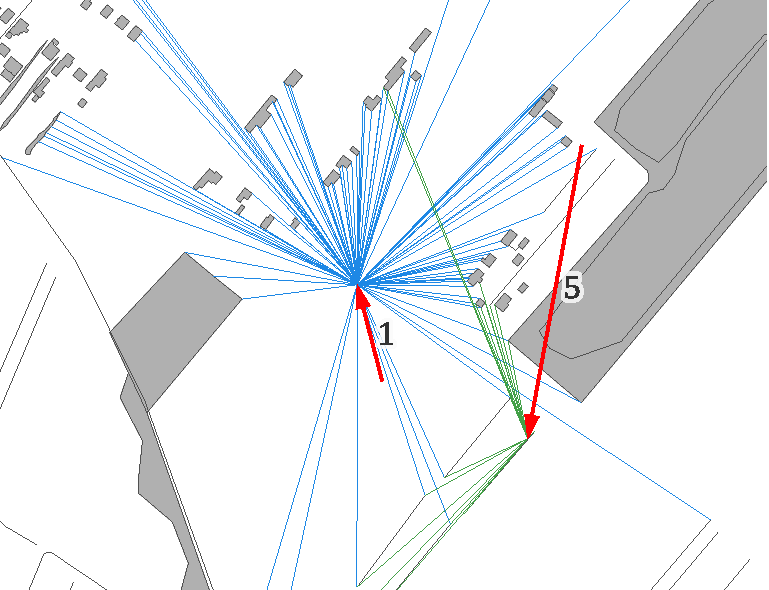
\includegraphics[width=\textwidth]{images/qgis-osm-rural}
				\end{minipage}
				\\
				\begin{minipage}[t]{0.4\textwidth}
					\captionof{table}{Measured values for the first and fifth routing requests illustrated in \Cref{fig:eval-osm-rural-map}.}
				\end{minipage}
				\hfill
				\begin{minipage}[t]{0.56\textwidth}
					\captionof{figure}{The first and fifth routing requests (red arrow between source and destination) with the nearby obstacles (gray). The bidirectional visibility edges of the two destinations are shown in blue and green.}
					\label{fig:eval-osm-rural-map}
				\end{minipage}
			\end{minipage}
			
		\subsubsection{Dataset without roads or obstacles}
		\label{subsubsec:dataset-without-roads-obstacles}
		
			The normal OSM-based datasets contain both, roads and obstacles.
			However, datasets containing only roads or only obstacles are thinkable and can also be used with the hybrid routing algorithm.
			For this evaluation, the 4km\textsuperscript{2} datasets of the \enquote{OSM city} and \enquote{OSM rural} categories were filtered yielding three datasets for each category:
			The normal dataset, one without roads and one without obstacles.
			In the dataset without roads, all road edges were removed which do not cross buildings, meaning building passages remained within this dataset to ensure the reachability of backyards.
			Influences of the two filters are discussed in the following.
			
			\begin{figure}[h!]
				\begin{figcenter}
					\begin{tabularx}{0.95\textwidth}{p{3cm}XXXp{2.25cm}X}
\toprule
\textbf{Operation}	& \textbf{Normal}	& \textbf{No roads}	& \textbf{Decrease compared to normal}	& \textbf{No obstacles}	& \textbf{Decrease compared to normal}	\\
\midrule
kNN search			& 315.86			& 288.69			&  8.60\%								& 0.000011				& 99.9999\%								\\
Create graph		&   0.69			&   0.68			&  0.84\%								& 0.000014				& 99.9999\%								\\
Get obstacles		&   0.30			&   0.29			&  3.28\%								& 0.0095				& 96.82\%								\\
Merge road edges	& 120.13			&  30.79			& 74.37\%								& 0.48					& 99.60\%								\\
Add POI attributes	&   0.054			&   0.025			& 53.81\%								& 0.008					& 85.97\%								\\
\midrule
Total time			& 437.34			& 320.57			& 26.70\%								& 0.53					& 99.88\%								\\
\bottomrule
					\end{tabularx}
				\end{figcenter}
				\vspace{3ex}
				\begin{figcenter}
					%% Creator: Matplotlib, PGF backend
%%
%% To include the figure in your LaTeX document, write
%%   \input{<filename>.pgf}
%%
%% Make sure the required packages are loaded in your preamble
%%   \usepackage{pgf}
%%
%% Also ensure that all the required font packages are loaded; for instance,
%% the lmodern package is sometimes necessary when using math font.
%%   \usepackage{lmodern}
%%
%% Figures using additional raster images can only be included by \input if
%% they are in the same directory as the main LaTeX file. For loading figures
%% from other directories you can use the `import` package
%%   \usepackage{import}
%%
%% and then include the figures with
%%   \import{<path to file>}{<filename>.pgf}
%%
%% Matplotlib used the following preamble
%%   
%%   \usepackage{fontspec}
%%   \setmainfont{DejaVuSerif.ttf}[Path=\detokenize{/home/hauke/.local/lib/python3.11/site-packages/matplotlib/mpl-data/fonts/ttf/}]
%%   \setsansfont{DroidSans.ttf}[Path=\detokenize{/usr/share/fonts/droid/}]
%%   \setmonofont{DejaVuSansMono.ttf}[Path=\detokenize{/home/hauke/.local/lib/python3.11/site-packages/matplotlib/mpl-data/fonts/ttf/}]
%%   \makeatletter\@ifpackageloaded{underscore}{}{\usepackage[strings]{underscore}}\makeatother
%%
\begingroup%
\makeatletter%
\begin{pgfpicture}%
\pgfpathrectangle{\pgfpointorigin}{\pgfqpoint{6.103826in}{1.704469in}}%
\pgfusepath{use as bounding box}%
\begin{pgfscope}%
\pgfsetbuttcap%
\pgfsetmiterjoin%
\definecolor{currentfill}{rgb}{1.000000,1.000000,1.000000}%
\pgfsetfillcolor{currentfill}%
\pgfsetlinewidth{0.000000pt}%
\definecolor{currentstroke}{rgb}{1.000000,1.000000,1.000000}%
\pgfsetstrokecolor{currentstroke}%
\pgfsetdash{}{0pt}%
\pgfpathmoveto{\pgfqpoint{0.000000in}{0.000000in}}%
\pgfpathlineto{\pgfqpoint{6.103826in}{0.000000in}}%
\pgfpathlineto{\pgfqpoint{6.103826in}{1.704469in}}%
\pgfpathlineto{\pgfqpoint{0.000000in}{1.704469in}}%
\pgfpathlineto{\pgfqpoint{0.000000in}{0.000000in}}%
\pgfpathclose%
\pgfusepath{fill}%
\end{pgfscope}%
\begin{pgfscope}%
\pgfsetbuttcap%
\pgfsetmiterjoin%
\definecolor{currentfill}{rgb}{1.000000,1.000000,1.000000}%
\pgfsetfillcolor{currentfill}%
\pgfsetlinewidth{0.000000pt}%
\definecolor{currentstroke}{rgb}{0.000000,0.000000,0.000000}%
\pgfsetstrokecolor{currentstroke}%
\pgfsetstrokeopacity{0.000000}%
\pgfsetdash{}{0pt}%
\pgfpathmoveto{\pgfqpoint{0.592976in}{0.595383in}}%
\pgfpathlineto{\pgfqpoint{4.767243in}{0.595383in}}%
\pgfpathlineto{\pgfqpoint{4.767243in}{1.704469in}}%
\pgfpathlineto{\pgfqpoint{0.592976in}{1.704469in}}%
\pgfpathlineto{\pgfqpoint{0.592976in}{0.595383in}}%
\pgfpathclose%
\pgfusepath{fill}%
\end{pgfscope}%
\begin{pgfscope}%
\definecolor{textcolor}{rgb}{0.150000,0.150000,0.150000}%
\pgfsetstrokecolor{textcolor}%
\pgfsetfillcolor{textcolor}%
\pgftext[x=0.940831in,y=0.463438in,,top]{\color{textcolor}\sffamily\fontsize{9.000000}{10.800000}\selectfont Total time}%
\end{pgfscope}%
\begin{pgfscope}%
\definecolor{textcolor}{rgb}{0.150000,0.150000,0.150000}%
\pgfsetstrokecolor{textcolor}%
\pgfsetfillcolor{textcolor}%
\pgftext[x=1.636543in,y=0.463438in,,top]{\color{textcolor}\sffamily\fontsize{9.000000}{10.800000}\selectfont kNN search}%
\end{pgfscope}%
\begin{pgfscope}%
\definecolor{textcolor}{rgb}{0.150000,0.150000,0.150000}%
\pgfsetstrokecolor{textcolor}%
\pgfsetfillcolor{textcolor}%
\pgftext[x=2.148385in, y=0.368467in, left, base]{\color{textcolor}\sffamily\fontsize{9.000000}{10.800000}\selectfont Create}%
\end{pgfscope}%
\begin{pgfscope}%
\definecolor{textcolor}{rgb}{0.150000,0.150000,0.150000}%
\pgfsetstrokecolor{textcolor}%
\pgfsetfillcolor{textcolor}%
\pgftext[x=2.168954in, y=0.224473in, left, base]{\color{textcolor}\sffamily\fontsize{9.000000}{10.800000}\selectfont graph}%
\end{pgfscope}%
\begin{pgfscope}%
\definecolor{textcolor}{rgb}{0.150000,0.150000,0.150000}%
\pgfsetstrokecolor{textcolor}%
\pgfsetfillcolor{textcolor}%
\pgftext[x=2.930217in, y=0.368467in, left, base]{\color{textcolor}\sffamily\fontsize{9.000000}{10.800000}\selectfont Get}%
\end{pgfscope}%
\begin{pgfscope}%
\definecolor{textcolor}{rgb}{0.150000,0.150000,0.150000}%
\pgfsetstrokecolor{textcolor}%
\pgfsetfillcolor{textcolor}%
\pgftext[x=2.765971in, y=0.224473in, left, base]{\color{textcolor}\sffamily\fontsize{9.000000}{10.800000}\selectfont obstacles}%
\end{pgfscope}%
\begin{pgfscope}%
\definecolor{textcolor}{rgb}{0.150000,0.150000,0.150000}%
\pgfsetstrokecolor{textcolor}%
\pgfsetfillcolor{textcolor}%
\pgftext[x=3.398664in, y=0.368467in, left, base]{\color{textcolor}\sffamily\fontsize{9.000000}{10.800000}\selectfont Merge road}%
\end{pgfscope}%
\begin{pgfscope}%
\definecolor{textcolor}{rgb}{0.150000,0.150000,0.150000}%
\pgfsetstrokecolor{textcolor}%
\pgfsetfillcolor{textcolor}%
\pgftext[x=3.559583in, y=0.224473in, left, base]{\color{textcolor}\sffamily\fontsize{9.000000}{10.800000}\selectfont edges}%
\end{pgfscope}%
\begin{pgfscope}%
\definecolor{textcolor}{rgb}{0.150000,0.150000,0.150000}%
\pgfsetstrokecolor{textcolor}%
\pgfsetfillcolor{textcolor}%
\pgftext[x=4.188949in, y=0.368467in, left, base]{\color{textcolor}\sffamily\fontsize{9.000000}{10.800000}\selectfont Add POI}%
\end{pgfscope}%
\begin{pgfscope}%
\definecolor{textcolor}{rgb}{0.150000,0.150000,0.150000}%
\pgfsetstrokecolor{textcolor}%
\pgfsetfillcolor{textcolor}%
\pgftext[x=4.145889in, y=0.224473in, left, base]{\color{textcolor}\sffamily\fontsize{9.000000}{10.800000}\selectfont attributes}%
\end{pgfscope}%
\begin{pgfscope}%
\definecolor{textcolor}{rgb}{0.150000,0.150000,0.150000}%
\pgfsetstrokecolor{textcolor}%
\pgfsetfillcolor{textcolor}%
\pgftext[x=2.680109in,y=0.125000in,,top]{\color{textcolor}\sffamily\fontsize{9.000000}{10.800000}\selectfont Input obstacle vertices}%
\end{pgfscope}%
\begin{pgfscope}%
\pgfpathrectangle{\pgfqpoint{0.592976in}{0.595383in}}{\pgfqpoint{4.174267in}{1.109087in}}%
\pgfusepath{clip}%
\pgfsetroundcap%
\pgfsetroundjoin%
\pgfsetlinewidth{1.003750pt}%
\definecolor{currentstroke}{rgb}{0.800000,0.800000,0.800000}%
\pgfsetstrokecolor{currentstroke}%
\pgfsetdash{}{0pt}%
\pgfpathmoveto{\pgfqpoint{0.592976in}{0.891511in}}%
\pgfpathlineto{\pgfqpoint{4.767243in}{0.891511in}}%
\pgfusepath{stroke}%
\end{pgfscope}%
\begin{pgfscope}%
\definecolor{textcolor}{rgb}{0.150000,0.150000,0.150000}%
\pgfsetstrokecolor{textcolor}%
\pgfsetfillcolor{textcolor}%
\pgftext[x=0.194444in, y=0.844025in, left, base]{\color{textcolor}\sffamily\fontsize{9.000000}{10.800000}\selectfont \(\displaystyle {10^{-3}}\)}%
\end{pgfscope}%
\begin{pgfscope}%
\pgfpathrectangle{\pgfqpoint{0.592976in}{0.595383in}}{\pgfqpoint{4.174267in}{1.109087in}}%
\pgfusepath{clip}%
\pgfsetroundcap%
\pgfsetroundjoin%
\pgfsetlinewidth{1.003750pt}%
\definecolor{currentstroke}{rgb}{0.800000,0.800000,0.800000}%
\pgfsetstrokecolor{currentstroke}%
\pgfsetdash{}{0pt}%
\pgfpathmoveto{\pgfqpoint{0.592976in}{1.273824in}}%
\pgfpathlineto{\pgfqpoint{4.767243in}{1.273824in}}%
\pgfusepath{stroke}%
\end{pgfscope}%
\begin{pgfscope}%
\definecolor{textcolor}{rgb}{0.150000,0.150000,0.150000}%
\pgfsetstrokecolor{textcolor}%
\pgfsetfillcolor{textcolor}%
\pgftext[x=0.274690in, y=1.226339in, left, base]{\color{textcolor}\sffamily\fontsize{9.000000}{10.800000}\selectfont \(\displaystyle {10^{0}}\)}%
\end{pgfscope}%
\begin{pgfscope}%
\pgfpathrectangle{\pgfqpoint{0.592976in}{0.595383in}}{\pgfqpoint{4.174267in}{1.109087in}}%
\pgfusepath{clip}%
\pgfsetroundcap%
\pgfsetroundjoin%
\pgfsetlinewidth{1.003750pt}%
\definecolor{currentstroke}{rgb}{0.800000,0.800000,0.800000}%
\pgfsetstrokecolor{currentstroke}%
\pgfsetdash{}{0pt}%
\pgfpathmoveto{\pgfqpoint{0.592976in}{1.656137in}}%
\pgfpathlineto{\pgfqpoint{4.767243in}{1.656137in}}%
\pgfusepath{stroke}%
\end{pgfscope}%
\begin{pgfscope}%
\definecolor{textcolor}{rgb}{0.150000,0.150000,0.150000}%
\pgfsetstrokecolor{textcolor}%
\pgfsetfillcolor{textcolor}%
\pgftext[x=0.274690in, y=1.608652in, left, base]{\color{textcolor}\sffamily\fontsize{9.000000}{10.800000}\selectfont \(\displaystyle {10^{3}}\)}%
\end{pgfscope}%
\begin{pgfscope}%
\definecolor{textcolor}{rgb}{0.150000,0.150000,0.150000}%
\pgfsetstrokecolor{textcolor}%
\pgfsetfillcolor{textcolor}%
\pgftext[x=0.125000in,y=1.149926in,,bottom,rotate=90.000000]{\color{textcolor}\sffamily\fontsize{9.000000}{10.800000}\selectfont Time in s}%
\end{pgfscope}%
\begin{pgfscope}%
\pgfpathrectangle{\pgfqpoint{0.592976in}{0.595383in}}{\pgfqpoint{4.174267in}{1.109087in}}%
\pgfusepath{clip}%
\pgfsetbuttcap%
\pgfsetmiterjoin%
\definecolor{currentfill}{rgb}{0.349020,0.490196,0.749020}%
\pgfsetfillcolor{currentfill}%
\pgfsetlinewidth{1.003750pt}%
\definecolor{currentstroke}{rgb}{1.000000,1.000000,1.000000}%
\pgfsetstrokecolor{currentstroke}%
\pgfsetdash{}{0pt}%
\pgfpathmoveto{\pgfqpoint{0.662547in}{-126.163917in}}%
\pgfpathlineto{\pgfqpoint{0.848070in}{-126.163917in}}%
\pgfpathlineto{\pgfqpoint{0.848070in}{1.654056in}}%
\pgfpathlineto{\pgfqpoint{0.662547in}{1.654056in}}%
\pgfpathlineto{\pgfqpoint{0.662547in}{-126.163917in}}%
\pgfpathclose%
\pgfusepath{stroke,fill}%
\end{pgfscope}%
\begin{pgfscope}%
\pgfpathrectangle{\pgfqpoint{0.592976in}{0.595383in}}{\pgfqpoint{4.174267in}{1.109087in}}%
\pgfusepath{clip}%
\pgfsetbuttcap%
\pgfsetmiterjoin%
\definecolor{currentfill}{rgb}{0.349020,0.490196,0.749020}%
\pgfsetfillcolor{currentfill}%
\pgfsetlinewidth{1.003750pt}%
\definecolor{currentstroke}{rgb}{1.000000,1.000000,1.000000}%
\pgfsetstrokecolor{currentstroke}%
\pgfsetdash{}{0pt}%
\pgfpathmoveto{\pgfqpoint{1.358258in}{-126.163917in}}%
\pgfpathlineto{\pgfqpoint{1.543781in}{-126.163917in}}%
\pgfpathlineto{\pgfqpoint{1.543781in}{1.621794in}}%
\pgfpathlineto{\pgfqpoint{1.358258in}{1.621794in}}%
\pgfpathlineto{\pgfqpoint{1.358258in}{-126.163917in}}%
\pgfpathclose%
\pgfusepath{stroke,fill}%
\end{pgfscope}%
\begin{pgfscope}%
\pgfpathrectangle{\pgfqpoint{0.592976in}{0.595383in}}{\pgfqpoint{4.174267in}{1.109087in}}%
\pgfusepath{clip}%
\pgfsetbuttcap%
\pgfsetmiterjoin%
\definecolor{currentfill}{rgb}{0.349020,0.490196,0.749020}%
\pgfsetfillcolor{currentfill}%
\pgfsetlinewidth{1.003750pt}%
\definecolor{currentstroke}{rgb}{1.000000,1.000000,1.000000}%
\pgfsetstrokecolor{currentstroke}%
\pgfsetdash{}{0pt}%
\pgfpathmoveto{\pgfqpoint{2.053969in}{-126.163917in}}%
\pgfpathlineto{\pgfqpoint{2.239492in}{-126.163917in}}%
\pgfpathlineto{\pgfqpoint{2.239492in}{1.282485in}}%
\pgfpathlineto{\pgfqpoint{2.053969in}{1.282485in}}%
\pgfpathlineto{\pgfqpoint{2.053969in}{-126.163917in}}%
\pgfpathclose%
\pgfusepath{stroke,fill}%
\end{pgfscope}%
\begin{pgfscope}%
\pgfpathrectangle{\pgfqpoint{0.592976in}{0.595383in}}{\pgfqpoint{4.174267in}{1.109087in}}%
\pgfusepath{clip}%
\pgfsetbuttcap%
\pgfsetmiterjoin%
\definecolor{currentfill}{rgb}{0.349020,0.490196,0.749020}%
\pgfsetfillcolor{currentfill}%
\pgfsetlinewidth{1.003750pt}%
\definecolor{currentstroke}{rgb}{1.000000,1.000000,1.000000}%
\pgfsetstrokecolor{currentstroke}%
\pgfsetdash{}{0pt}%
\pgfpathmoveto{\pgfqpoint{2.749680in}{-126.163917in}}%
\pgfpathlineto{\pgfqpoint{2.935203in}{-126.163917in}}%
\pgfpathlineto{\pgfqpoint{2.935203in}{1.184746in}}%
\pgfpathlineto{\pgfqpoint{2.749680in}{1.184746in}}%
\pgfpathlineto{\pgfqpoint{2.749680in}{-126.163917in}}%
\pgfpathclose%
\pgfusepath{stroke,fill}%
\end{pgfscope}%
\begin{pgfscope}%
\pgfpathrectangle{\pgfqpoint{0.592976in}{0.595383in}}{\pgfqpoint{4.174267in}{1.109087in}}%
\pgfusepath{clip}%
\pgfsetbuttcap%
\pgfsetmiterjoin%
\definecolor{currentfill}{rgb}{0.349020,0.490196,0.749020}%
\pgfsetfillcolor{currentfill}%
\pgfsetlinewidth{1.003750pt}%
\definecolor{currentstroke}{rgb}{1.000000,1.000000,1.000000}%
\pgfsetstrokecolor{currentstroke}%
\pgfsetdash{}{0pt}%
\pgfpathmoveto{\pgfqpoint{3.445391in}{-126.163917in}}%
\pgfpathlineto{\pgfqpoint{3.630914in}{-126.163917in}}%
\pgfpathlineto{\pgfqpoint{3.630914in}{1.608561in}}%
\pgfpathlineto{\pgfqpoint{3.445391in}{1.608561in}}%
\pgfpathlineto{\pgfqpoint{3.445391in}{-126.163917in}}%
\pgfpathclose%
\pgfusepath{stroke,fill}%
\end{pgfscope}%
\begin{pgfscope}%
\pgfpathrectangle{\pgfqpoint{0.592976in}{0.595383in}}{\pgfqpoint{4.174267in}{1.109087in}}%
\pgfusepath{clip}%
\pgfsetbuttcap%
\pgfsetmiterjoin%
\definecolor{currentfill}{rgb}{0.349020,0.490196,0.749020}%
\pgfsetfillcolor{currentfill}%
\pgfsetlinewidth{1.003750pt}%
\definecolor{currentstroke}{rgb}{1.000000,1.000000,1.000000}%
\pgfsetstrokecolor{currentstroke}%
\pgfsetdash{}{0pt}%
\pgfpathmoveto{\pgfqpoint{4.141103in}{-126.163917in}}%
\pgfpathlineto{\pgfqpoint{4.326626in}{-126.163917in}}%
\pgfpathlineto{\pgfqpoint{4.326626in}{1.116913in}}%
\pgfpathlineto{\pgfqpoint{4.141103in}{1.116913in}}%
\pgfpathlineto{\pgfqpoint{4.141103in}{-126.163917in}}%
\pgfpathclose%
\pgfusepath{stroke,fill}%
\end{pgfscope}%
\begin{pgfscope}%
\pgfpathrectangle{\pgfqpoint{0.592976in}{0.595383in}}{\pgfqpoint{4.174267in}{1.109087in}}%
\pgfusepath{clip}%
\pgfsetbuttcap%
\pgfsetmiterjoin%
\definecolor{currentfill}{rgb}{0.852941,0.544118,0.370588}%
\pgfsetfillcolor{currentfill}%
\pgfsetlinewidth{1.003750pt}%
\definecolor{currentstroke}{rgb}{1.000000,1.000000,1.000000}%
\pgfsetstrokecolor{currentstroke}%
\pgfsetdash{}{0pt}%
\pgfpathmoveto{\pgfqpoint{0.848070in}{-126.163917in}}%
\pgfpathlineto{\pgfqpoint{1.033593in}{-126.163917in}}%
\pgfpathlineto{\pgfqpoint{1.033593in}{1.621550in}}%
\pgfpathlineto{\pgfqpoint{0.848070in}{1.621550in}}%
\pgfpathlineto{\pgfqpoint{0.848070in}{-126.163917in}}%
\pgfpathclose%
\pgfusepath{stroke,fill}%
\end{pgfscope}%
\begin{pgfscope}%
\pgfpathrectangle{\pgfqpoint{0.592976in}{0.595383in}}{\pgfqpoint{4.174267in}{1.109087in}}%
\pgfusepath{clip}%
\pgfsetbuttcap%
\pgfsetmiterjoin%
\definecolor{currentfill}{rgb}{0.852941,0.544118,0.370588}%
\pgfsetfillcolor{currentfill}%
\pgfsetlinewidth{1.003750pt}%
\definecolor{currentstroke}{rgb}{1.000000,1.000000,1.000000}%
\pgfsetstrokecolor{currentstroke}%
\pgfsetdash{}{0pt}%
\pgfpathmoveto{\pgfqpoint{1.543781in}{-126.163917in}}%
\pgfpathlineto{\pgfqpoint{1.729304in}{-126.163917in}}%
\pgfpathlineto{\pgfqpoint{1.729304in}{1.619104in}}%
\pgfpathlineto{\pgfqpoint{1.543781in}{1.619104in}}%
\pgfpathlineto{\pgfqpoint{1.543781in}{-126.163917in}}%
\pgfpathclose%
\pgfusepath{stroke,fill}%
\end{pgfscope}%
\begin{pgfscope}%
\pgfpathrectangle{\pgfqpoint{0.592976in}{0.595383in}}{\pgfqpoint{4.174267in}{1.109087in}}%
\pgfusepath{clip}%
\pgfsetbuttcap%
\pgfsetmiterjoin%
\definecolor{currentfill}{rgb}{0.852941,0.544118,0.370588}%
\pgfsetfillcolor{currentfill}%
\pgfsetlinewidth{1.003750pt}%
\definecolor{currentstroke}{rgb}{1.000000,1.000000,1.000000}%
\pgfsetstrokecolor{currentstroke}%
\pgfsetdash{}{0pt}%
\pgfpathmoveto{\pgfqpoint{2.239492in}{-126.163917in}}%
\pgfpathlineto{\pgfqpoint{2.425015in}{-126.163917in}}%
\pgfpathlineto{\pgfqpoint{2.425015in}{1.276251in}}%
\pgfpathlineto{\pgfqpoint{2.239492in}{1.276251in}}%
\pgfpathlineto{\pgfqpoint{2.239492in}{-126.163917in}}%
\pgfpathclose%
\pgfusepath{stroke,fill}%
\end{pgfscope}%
\begin{pgfscope}%
\pgfpathrectangle{\pgfqpoint{0.592976in}{0.595383in}}{\pgfqpoint{4.174267in}{1.109087in}}%
\pgfusepath{clip}%
\pgfsetbuttcap%
\pgfsetmiterjoin%
\definecolor{currentfill}{rgb}{0.852941,0.544118,0.370588}%
\pgfsetfillcolor{currentfill}%
\pgfsetlinewidth{1.003750pt}%
\definecolor{currentstroke}{rgb}{1.000000,1.000000,1.000000}%
\pgfsetstrokecolor{currentstroke}%
\pgfsetdash{}{0pt}%
\pgfpathmoveto{\pgfqpoint{2.935203in}{-126.163917in}}%
\pgfpathlineto{\pgfqpoint{3.120726in}{-126.163917in}}%
\pgfpathlineto{\pgfqpoint{3.120726in}{1.185267in}}%
\pgfpathlineto{\pgfqpoint{2.935203in}{1.185267in}}%
\pgfpathlineto{\pgfqpoint{2.935203in}{-126.163917in}}%
\pgfpathclose%
\pgfusepath{stroke,fill}%
\end{pgfscope}%
\begin{pgfscope}%
\pgfpathrectangle{\pgfqpoint{0.592976in}{0.595383in}}{\pgfqpoint{4.174267in}{1.109087in}}%
\pgfusepath{clip}%
\pgfsetbuttcap%
\pgfsetmiterjoin%
\definecolor{currentfill}{rgb}{0.852941,0.544118,0.370588}%
\pgfsetfillcolor{currentfill}%
\pgfsetlinewidth{1.003750pt}%
\definecolor{currentstroke}{rgb}{1.000000,1.000000,1.000000}%
\pgfsetstrokecolor{currentstroke}%
\pgfsetdash{}{0pt}%
\pgfpathmoveto{\pgfqpoint{3.630914in}{-126.163917in}}%
\pgfpathlineto{\pgfqpoint{3.816437in}{-126.163917in}}%
\pgfpathlineto{\pgfqpoint{3.816437in}{1.444306in}}%
\pgfpathlineto{\pgfqpoint{3.630914in}{1.444306in}}%
\pgfpathlineto{\pgfqpoint{3.630914in}{-126.163917in}}%
\pgfpathclose%
\pgfusepath{stroke,fill}%
\end{pgfscope}%
\begin{pgfscope}%
\pgfpathrectangle{\pgfqpoint{0.592976in}{0.595383in}}{\pgfqpoint{4.174267in}{1.109087in}}%
\pgfusepath{clip}%
\pgfsetbuttcap%
\pgfsetmiterjoin%
\definecolor{currentfill}{rgb}{0.852941,0.544118,0.370588}%
\pgfsetfillcolor{currentfill}%
\pgfsetlinewidth{1.003750pt}%
\definecolor{currentstroke}{rgb}{1.000000,1.000000,1.000000}%
\pgfsetstrokecolor{currentstroke}%
\pgfsetdash{}{0pt}%
\pgfpathmoveto{\pgfqpoint{4.326626in}{-126.163917in}}%
\pgfpathlineto{\pgfqpoint{4.512149in}{-126.163917in}}%
\pgfpathlineto{\pgfqpoint{4.512149in}{1.084764in}}%
\pgfpathlineto{\pgfqpoint{4.326626in}{1.084764in}}%
\pgfpathlineto{\pgfqpoint{4.326626in}{-126.163917in}}%
\pgfpathclose%
\pgfusepath{stroke,fill}%
\end{pgfscope}%
\begin{pgfscope}%
\pgfpathrectangle{\pgfqpoint{0.592976in}{0.595383in}}{\pgfqpoint{4.174267in}{1.109087in}}%
\pgfusepath{clip}%
\pgfsetbuttcap%
\pgfsetmiterjoin%
\definecolor{currentfill}{rgb}{0.460784,0.749020,0.443137}%
\pgfsetfillcolor{currentfill}%
\pgfsetlinewidth{1.003750pt}%
\definecolor{currentstroke}{rgb}{1.000000,1.000000,1.000000}%
\pgfsetstrokecolor{currentstroke}%
\pgfsetdash{}{0pt}%
\pgfpathmoveto{\pgfqpoint{1.033593in}{-126.163917in}}%
\pgfpathlineto{\pgfqpoint{1.219116in}{-126.163917in}}%
\pgfpathlineto{\pgfqpoint{1.219116in}{1.293809in}}%
\pgfpathlineto{\pgfqpoint{1.033593in}{1.293809in}}%
\pgfpathlineto{\pgfqpoint{1.033593in}{-126.163917in}}%
\pgfpathclose%
\pgfusepath{stroke,fill}%
\end{pgfscope}%
\begin{pgfscope}%
\pgfpathrectangle{\pgfqpoint{0.592976in}{0.595383in}}{\pgfqpoint{4.174267in}{1.109087in}}%
\pgfusepath{clip}%
\pgfsetbuttcap%
\pgfsetmiterjoin%
\definecolor{currentfill}{rgb}{0.460784,0.749020,0.443137}%
\pgfsetfillcolor{currentfill}%
\pgfsetlinewidth{1.003750pt}%
\definecolor{currentstroke}{rgb}{1.000000,1.000000,1.000000}%
\pgfsetstrokecolor{currentstroke}%
\pgfsetdash{}{0pt}%
\pgfpathmoveto{\pgfqpoint{1.729304in}{-126.163917in}}%
\pgfpathlineto{\pgfqpoint{1.914827in}{-126.163917in}}%
\pgfpathlineto{\pgfqpoint{1.914827in}{0.645796in}}%
\pgfpathlineto{\pgfqpoint{1.729304in}{0.645796in}}%
\pgfpathlineto{\pgfqpoint{1.729304in}{-126.163917in}}%
\pgfpathclose%
\pgfusepath{stroke,fill}%
\end{pgfscope}%
\begin{pgfscope}%
\pgfpathrectangle{\pgfqpoint{0.592976in}{0.595383in}}{\pgfqpoint{4.174267in}{1.109087in}}%
\pgfusepath{clip}%
\pgfsetbuttcap%
\pgfsetmiterjoin%
\definecolor{currentfill}{rgb}{0.460784,0.749020,0.443137}%
\pgfsetfillcolor{currentfill}%
\pgfsetlinewidth{1.003750pt}%
\definecolor{currentstroke}{rgb}{1.000000,1.000000,1.000000}%
\pgfsetstrokecolor{currentstroke}%
\pgfsetdash{}{0pt}%
\pgfpathmoveto{\pgfqpoint{2.425015in}{-126.163917in}}%
\pgfpathlineto{\pgfqpoint{2.610538in}{-126.163917in}}%
\pgfpathlineto{\pgfqpoint{2.610538in}{0.652833in}}%
\pgfpathlineto{\pgfqpoint{2.425015in}{0.652833in}}%
\pgfpathlineto{\pgfqpoint{2.425015in}{-126.163917in}}%
\pgfpathclose%
\pgfusepath{stroke,fill}%
\end{pgfscope}%
\begin{pgfscope}%
\pgfpathrectangle{\pgfqpoint{0.592976in}{0.595383in}}{\pgfqpoint{4.174267in}{1.109087in}}%
\pgfusepath{clip}%
\pgfsetbuttcap%
\pgfsetmiterjoin%
\definecolor{currentfill}{rgb}{0.460784,0.749020,0.443137}%
\pgfsetfillcolor{currentfill}%
\pgfsetlinewidth{1.003750pt}%
\definecolor{currentstroke}{rgb}{1.000000,1.000000,1.000000}%
\pgfsetstrokecolor{currentstroke}%
\pgfsetdash{}{0pt}%
\pgfpathmoveto{\pgfqpoint{3.120726in}{-126.163917in}}%
\pgfpathlineto{\pgfqpoint{3.306249in}{-126.163917in}}%
\pgfpathlineto{\pgfqpoint{3.306249in}{1.020032in}}%
\pgfpathlineto{\pgfqpoint{3.120726in}{1.020032in}}%
\pgfpathlineto{\pgfqpoint{3.120726in}{-126.163917in}}%
\pgfpathclose%
\pgfusepath{stroke,fill}%
\end{pgfscope}%
\begin{pgfscope}%
\pgfpathrectangle{\pgfqpoint{0.592976in}{0.595383in}}{\pgfqpoint{4.174267in}{1.109087in}}%
\pgfusepath{clip}%
\pgfsetbuttcap%
\pgfsetmiterjoin%
\definecolor{currentfill}{rgb}{0.460784,0.749020,0.443137}%
\pgfsetfillcolor{currentfill}%
\pgfsetlinewidth{1.003750pt}%
\definecolor{currentstroke}{rgb}{1.000000,1.000000,1.000000}%
\pgfsetstrokecolor{currentstroke}%
\pgfsetdash{}{0pt}%
\pgfpathmoveto{\pgfqpoint{3.816437in}{-126.163917in}}%
\pgfpathlineto{\pgfqpoint{4.001960in}{-126.163917in}}%
\pgfpathlineto{\pgfqpoint{4.001960in}{1.291903in}}%
\pgfpathlineto{\pgfqpoint{3.816437in}{1.291903in}}%
\pgfpathlineto{\pgfqpoint{3.816437in}{-126.163917in}}%
\pgfpathclose%
\pgfusepath{stroke,fill}%
\end{pgfscope}%
\begin{pgfscope}%
\pgfpathrectangle{\pgfqpoint{0.592976in}{0.595383in}}{\pgfqpoint{4.174267in}{1.109087in}}%
\pgfusepath{clip}%
\pgfsetbuttcap%
\pgfsetmiterjoin%
\definecolor{currentfill}{rgb}{0.460784,0.749020,0.443137}%
\pgfsetfillcolor{currentfill}%
\pgfsetlinewidth{1.003750pt}%
\definecolor{currentstroke}{rgb}{1.000000,1.000000,1.000000}%
\pgfsetstrokecolor{currentstroke}%
\pgfsetdash{}{0pt}%
\pgfpathmoveto{\pgfqpoint{4.512149in}{-126.163917in}}%
\pgfpathlineto{\pgfqpoint{4.697672in}{-126.163917in}}%
\pgfpathlineto{\pgfqpoint{4.697672in}{1.028773in}}%
\pgfpathlineto{\pgfqpoint{4.512149in}{1.028773in}}%
\pgfpathlineto{\pgfqpoint{4.512149in}{-126.163917in}}%
\pgfpathclose%
\pgfusepath{stroke,fill}%
\end{pgfscope}%
\begin{pgfscope}%
\pgfsetrectcap%
\pgfsetmiterjoin%
\pgfsetlinewidth{1.254687pt}%
\definecolor{currentstroke}{rgb}{0.800000,0.800000,0.800000}%
\pgfsetstrokecolor{currentstroke}%
\pgfsetdash{}{0pt}%
\pgfpathmoveto{\pgfqpoint{0.592976in}{0.595383in}}%
\pgfpathlineto{\pgfqpoint{0.592976in}{1.704469in}}%
\pgfusepath{stroke}%
\end{pgfscope}%
\begin{pgfscope}%
\pgfsetrectcap%
\pgfsetmiterjoin%
\pgfsetlinewidth{1.254687pt}%
\definecolor{currentstroke}{rgb}{0.800000,0.800000,0.800000}%
\pgfsetstrokecolor{currentstroke}%
\pgfsetdash{}{0pt}%
\pgfpathmoveto{\pgfqpoint{4.767243in}{0.595383in}}%
\pgfpathlineto{\pgfqpoint{4.767243in}{1.704469in}}%
\pgfusepath{stroke}%
\end{pgfscope}%
\begin{pgfscope}%
\pgfsetrectcap%
\pgfsetmiterjoin%
\pgfsetlinewidth{1.254687pt}%
\definecolor{currentstroke}{rgb}{0.800000,0.800000,0.800000}%
\pgfsetstrokecolor{currentstroke}%
\pgfsetdash{}{0pt}%
\pgfpathmoveto{\pgfqpoint{0.592976in}{0.595383in}}%
\pgfpathlineto{\pgfqpoint{4.767243in}{0.595383in}}%
\pgfusepath{stroke}%
\end{pgfscope}%
\begin{pgfscope}%
\pgfsetrectcap%
\pgfsetmiterjoin%
\pgfsetlinewidth{1.254687pt}%
\definecolor{currentstroke}{rgb}{0.800000,0.800000,0.800000}%
\pgfsetstrokecolor{currentstroke}%
\pgfsetdash{}{0pt}%
\pgfpathmoveto{\pgfqpoint{0.592976in}{1.704469in}}%
\pgfpathlineto{\pgfqpoint{4.767243in}{1.704469in}}%
\pgfusepath{stroke}%
\end{pgfscope}%
\begin{pgfscope}%
\pgfsetbuttcap%
\pgfsetmiterjoin%
\definecolor{currentfill}{rgb}{1.000000,1.000000,1.000000}%
\pgfsetfillcolor{currentfill}%
\pgfsetfillopacity{0.800000}%
\pgfsetlinewidth{1.003750pt}%
\definecolor{currentstroke}{rgb}{0.800000,0.800000,0.800000}%
\pgfsetstrokecolor{currentstroke}%
\pgfsetstrokeopacity{0.800000}%
\pgfsetdash{}{0pt}%
\pgfpathmoveto{\pgfqpoint{4.959099in}{0.756176in}}%
\pgfpathlineto{\pgfqpoint{6.078826in}{0.756176in}}%
\pgfpathquadraticcurveto{\pgfqpoint{6.103826in}{0.756176in}}{\pgfqpoint{6.103826in}{0.781176in}}%
\pgfpathlineto{\pgfqpoint{6.103826in}{1.518676in}}%
\pgfpathquadraticcurveto{\pgfqpoint{6.103826in}{1.543676in}}{\pgfqpoint{6.078826in}{1.543676in}}%
\pgfpathlineto{\pgfqpoint{4.959099in}{1.543676in}}%
\pgfpathquadraticcurveto{\pgfqpoint{4.934099in}{1.543676in}}{\pgfqpoint{4.934099in}{1.518676in}}%
\pgfpathlineto{\pgfqpoint{4.934099in}{0.781176in}}%
\pgfpathquadraticcurveto{\pgfqpoint{4.934099in}{0.756176in}}{\pgfqpoint{4.959099in}{0.756176in}}%
\pgfpathlineto{\pgfqpoint{4.959099in}{0.756176in}}%
\pgfpathclose%
\pgfusepath{stroke,fill}%
\end{pgfscope}%
\begin{pgfscope}%
\definecolor{textcolor}{rgb}{0.150000,0.150000,0.150000}%
\pgfsetstrokecolor{textcolor}%
\pgfsetfillcolor{textcolor}%
\pgftext[x=5.305858in,y=1.398705in,left,base]{\color{textcolor}\sffamily\fontsize{9.000000}{10.800000}\selectfont Dataset}%
\end{pgfscope}%
\begin{pgfscope}%
\pgfsetbuttcap%
\pgfsetmiterjoin%
\definecolor{currentfill}{rgb}{0.349020,0.490196,0.749020}%
\pgfsetfillcolor{currentfill}%
\pgfsetlinewidth{1.003750pt}%
\definecolor{currentstroke}{rgb}{1.000000,1.000000,1.000000}%
\pgfsetstrokecolor{currentstroke}%
\pgfsetdash{}{0pt}%
\pgfpathmoveto{\pgfqpoint{4.984099in}{1.211205in}}%
\pgfpathlineto{\pgfqpoint{5.234099in}{1.211205in}}%
\pgfpathlineto{\pgfqpoint{5.234099in}{1.298705in}}%
\pgfpathlineto{\pgfqpoint{4.984099in}{1.298705in}}%
\pgfpathlineto{\pgfqpoint{4.984099in}{1.211205in}}%
\pgfpathclose%
\pgfusepath{stroke,fill}%
\end{pgfscope}%
\begin{pgfscope}%
\definecolor{textcolor}{rgb}{0.150000,0.150000,0.150000}%
\pgfsetstrokecolor{textcolor}%
\pgfsetfillcolor{textcolor}%
\pgftext[x=5.334099in,y=1.211205in,left,base]{\color{textcolor}\sffamily\fontsize{9.000000}{10.800000}\selectfont Normal}%
\end{pgfscope}%
\begin{pgfscope}%
\pgfsetbuttcap%
\pgfsetmiterjoin%
\definecolor{currentfill}{rgb}{0.852941,0.544118,0.370588}%
\pgfsetfillcolor{currentfill}%
\pgfsetlinewidth{1.003750pt}%
\definecolor{currentstroke}{rgb}{1.000000,1.000000,1.000000}%
\pgfsetstrokecolor{currentstroke}%
\pgfsetdash{}{0pt}%
\pgfpathmoveto{\pgfqpoint{4.984099in}{1.023705in}}%
\pgfpathlineto{\pgfqpoint{5.234099in}{1.023705in}}%
\pgfpathlineto{\pgfqpoint{5.234099in}{1.111205in}}%
\pgfpathlineto{\pgfqpoint{4.984099in}{1.111205in}}%
\pgfpathlineto{\pgfqpoint{4.984099in}{1.023705in}}%
\pgfpathclose%
\pgfusepath{stroke,fill}%
\end{pgfscope}%
\begin{pgfscope}%
\definecolor{textcolor}{rgb}{0.150000,0.150000,0.150000}%
\pgfsetstrokecolor{textcolor}%
\pgfsetfillcolor{textcolor}%
\pgftext[x=5.334099in,y=1.023705in,left,base]{\color{textcolor}\sffamily\fontsize{9.000000}{10.800000}\selectfont No roads}%
\end{pgfscope}%
\begin{pgfscope}%
\pgfsetbuttcap%
\pgfsetmiterjoin%
\definecolor{currentfill}{rgb}{0.460784,0.749020,0.443137}%
\pgfsetfillcolor{currentfill}%
\pgfsetlinewidth{1.003750pt}%
\definecolor{currentstroke}{rgb}{1.000000,1.000000,1.000000}%
\pgfsetstrokecolor{currentstroke}%
\pgfsetdash{}{0pt}%
\pgfpathmoveto{\pgfqpoint{4.984099in}{0.836205in}}%
\pgfpathlineto{\pgfqpoint{5.234099in}{0.836205in}}%
\pgfpathlineto{\pgfqpoint{5.234099in}{0.923705in}}%
\pgfpathlineto{\pgfqpoint{4.984099in}{0.923705in}}%
\pgfpathlineto{\pgfqpoint{4.984099in}{0.836205in}}%
\pgfpathclose%
\pgfusepath{stroke,fill}%
\end{pgfscope}%
\begin{pgfscope}%
\definecolor{textcolor}{rgb}{0.150000,0.150000,0.150000}%
\pgfsetstrokecolor{textcolor}%
\pgfsetfillcolor{textcolor}%
\pgftext[x=5.334099in,y=0.836205in,left,base]{\color{textcolor}\sffamily\fontsize{9.000000}{10.800000}\selectfont No obstacles}%
\end{pgfscope}%
\end{pgfpicture}%
\makeatother%
\endgroup%

				\end{figcenter}
				\caption{Comparison of the normal 4km\textsuperscript{2} \enquote{OSM city} dataset (blue) with the same dataset but without roads (orange) and without obstacles (green). All numbers in the table are given in seconds.}
				\label{fig:eval-import-osm-no-roads-obstacles-city}
			\end{figure}
			
			\Cref{fig:eval-import-osm-no-roads-obstacles-city} lists and illustrates the results for the \enquote{OSM city} datasets.
			Some noteworthy insights can be inferred from these data:
			\begin{itemize}
				\item The kNN search and visibility graph creation times were significantly reduced for the dataset without obstacles, which is expected, since both operations take only obstacles into account.
				\item The merge operation for the dataset without roads took longer compared to the dataset without obstacles.
				This is due to the 175 remaining building passages within the \enquote{no roads} dataset, which means this operation still merges road edges and therefore requires some time.
				However, compared to the normal dataset the merge operation only required 25.63\% of the time in the \enquote{no road} dataset, which does not match the number of remaining road edges of 4.82\% (175 edges) compared to the normal dataset (3629 edges).
				Because building passages consist of short segments, their start and end vertices needs to be connected to the rest of the graph.
				This is the case for 742 such dead-end vertices in the normal dataset and for 346 in the dataset without roads, which yields the relatively, with respect to the number of edges, long processing time.
				\item In the \enquote{no obstacles} dataset the merge operation took 0.4\% of the normal time. This is expected, because no visibility graph edges exist and therefore to merge between visibility edges and road edges takes place.
			\end{itemize}
			
			\begin{figure}[h!]
				\begin{tabularx}{0.95\textwidth}{p{3cm}XXXp{2.25cm}X}
\toprule
\textbf{Operation}	& \textbf{Normal}	& \textbf{No roads}	& \textbf{Decrease compared to normal}	& \textbf{No obstacles}	& \textbf{Decrease compared to normal}	\\
\midrule
kNN search			&  5,958			& 5,924				&   0.57\%								&  0.0094				& 99.9998\%								\\
Create graph		&    191.68			&   210.4			&  -9.76\%								&  0.012				& 99.9936\%								\\
Get obstacles		&     42.53			&    40.76			&   4.15\%								&  0.78					& 98.16\%								\\
Merge road edges	&  6,600			&     5.67			&  99.91\%								& 32.79					& 99.5\%								\\
Add POI attributes	&      4.83			&     1.53			&  68.21\%								&  0.42					& 91.26\%								\\
\midrule
Total time			& 12,854			& 6,202				&  51.75\%								& 37.19					& 99.71\%								\\
\bottomrule
				\end{tabularx}
				\vspace{3ex}
				\begin{figcenter}
					%% Creator: Matplotlib, PGF backend
%%
%% To include the figure in your LaTeX document, write
%%   \input{<filename>.pgf}
%%
%% Make sure the required packages are loaded in your preamble
%%   \usepackage{pgf}
%%
%% Also ensure that all the required font packages are loaded; for instance,
%% the lmodern package is sometimes necessary when using math font.
%%   \usepackage{lmodern}
%%
%% Figures using additional raster images can only be included by \input if
%% they are in the same directory as the main LaTeX file. For loading figures
%% from other directories you can use the `import` package
%%   \usepackage{import}
%%
%% and then include the figures with
%%   \import{<path to file>}{<filename>.pgf}
%%
%% Matplotlib used the following preamble
%%   
%%   \usepackage{fontspec}
%%   \setmainfont{DejaVuSerif.ttf}[Path=\detokenize{/home/hauke/.local/lib/python3.11/site-packages/matplotlib/mpl-data/fonts/ttf/}]
%%   \setsansfont{DroidSans.ttf}[Path=\detokenize{/usr/share/fonts/droid/}]
%%   \setmonofont{DejaVuSansMono.ttf}[Path=\detokenize{/home/hauke/.local/lib/python3.11/site-packages/matplotlib/mpl-data/fonts/ttf/}]
%%   \makeatletter\@ifpackageloaded{underscore}{}{\usepackage[strings]{underscore}}\makeatother
%%
\begingroup%
\makeatletter%
\begin{pgfpicture}%
\pgfpathrectangle{\pgfpointorigin}{\pgfqpoint{6.103826in}{1.704469in}}%
\pgfusepath{use as bounding box}%
\begin{pgfscope}%
\pgfsetbuttcap%
\pgfsetmiterjoin%
\definecolor{currentfill}{rgb}{1.000000,1.000000,1.000000}%
\pgfsetfillcolor{currentfill}%
\pgfsetlinewidth{0.000000pt}%
\definecolor{currentstroke}{rgb}{1.000000,1.000000,1.000000}%
\pgfsetstrokecolor{currentstroke}%
\pgfsetdash{}{0pt}%
\pgfpathmoveto{\pgfqpoint{0.000000in}{0.000000in}}%
\pgfpathlineto{\pgfqpoint{6.103826in}{0.000000in}}%
\pgfpathlineto{\pgfqpoint{6.103826in}{1.704469in}}%
\pgfpathlineto{\pgfqpoint{0.000000in}{1.704469in}}%
\pgfpathlineto{\pgfqpoint{0.000000in}{0.000000in}}%
\pgfpathclose%
\pgfusepath{fill}%
\end{pgfscope}%
\begin{pgfscope}%
\pgfsetbuttcap%
\pgfsetmiterjoin%
\definecolor{currentfill}{rgb}{1.000000,1.000000,1.000000}%
\pgfsetfillcolor{currentfill}%
\pgfsetlinewidth{0.000000pt}%
\definecolor{currentstroke}{rgb}{0.000000,0.000000,0.000000}%
\pgfsetstrokecolor{currentstroke}%
\pgfsetstrokeopacity{0.000000}%
\pgfsetdash{}{0pt}%
\pgfpathmoveto{\pgfqpoint{0.592976in}{0.595383in}}%
\pgfpathlineto{\pgfqpoint{4.767243in}{0.595383in}}%
\pgfpathlineto{\pgfqpoint{4.767243in}{1.704469in}}%
\pgfpathlineto{\pgfqpoint{0.592976in}{1.704469in}}%
\pgfpathlineto{\pgfqpoint{0.592976in}{0.595383in}}%
\pgfpathclose%
\pgfusepath{fill}%
\end{pgfscope}%
\begin{pgfscope}%
\definecolor{textcolor}{rgb}{0.150000,0.150000,0.150000}%
\pgfsetstrokecolor{textcolor}%
\pgfsetfillcolor{textcolor}%
\pgftext[x=0.940831in,y=0.463438in,,top]{\color{textcolor}\sffamily\fontsize{9.000000}{10.800000}\selectfont Total time}%
\end{pgfscope}%
\begin{pgfscope}%
\definecolor{textcolor}{rgb}{0.150000,0.150000,0.150000}%
\pgfsetstrokecolor{textcolor}%
\pgfsetfillcolor{textcolor}%
\pgftext[x=1.636543in,y=0.463438in,,top]{\color{textcolor}\sffamily\fontsize{9.000000}{10.800000}\selectfont kNN search}%
\end{pgfscope}%
\begin{pgfscope}%
\definecolor{textcolor}{rgb}{0.150000,0.150000,0.150000}%
\pgfsetstrokecolor{textcolor}%
\pgfsetfillcolor{textcolor}%
\pgftext[x=2.148385in, y=0.368467in, left, base]{\color{textcolor}\sffamily\fontsize{9.000000}{10.800000}\selectfont Create}%
\end{pgfscope}%
\begin{pgfscope}%
\definecolor{textcolor}{rgb}{0.150000,0.150000,0.150000}%
\pgfsetstrokecolor{textcolor}%
\pgfsetfillcolor{textcolor}%
\pgftext[x=2.168954in, y=0.224473in, left, base]{\color{textcolor}\sffamily\fontsize{9.000000}{10.800000}\selectfont graph}%
\end{pgfscope}%
\begin{pgfscope}%
\definecolor{textcolor}{rgb}{0.150000,0.150000,0.150000}%
\pgfsetstrokecolor{textcolor}%
\pgfsetfillcolor{textcolor}%
\pgftext[x=2.930217in, y=0.368467in, left, base]{\color{textcolor}\sffamily\fontsize{9.000000}{10.800000}\selectfont Get}%
\end{pgfscope}%
\begin{pgfscope}%
\definecolor{textcolor}{rgb}{0.150000,0.150000,0.150000}%
\pgfsetstrokecolor{textcolor}%
\pgfsetfillcolor{textcolor}%
\pgftext[x=2.765971in, y=0.224473in, left, base]{\color{textcolor}\sffamily\fontsize{9.000000}{10.800000}\selectfont obstacles}%
\end{pgfscope}%
\begin{pgfscope}%
\definecolor{textcolor}{rgb}{0.150000,0.150000,0.150000}%
\pgfsetstrokecolor{textcolor}%
\pgfsetfillcolor{textcolor}%
\pgftext[x=3.398664in, y=0.368467in, left, base]{\color{textcolor}\sffamily\fontsize{9.000000}{10.800000}\selectfont Merge road}%
\end{pgfscope}%
\begin{pgfscope}%
\definecolor{textcolor}{rgb}{0.150000,0.150000,0.150000}%
\pgfsetstrokecolor{textcolor}%
\pgfsetfillcolor{textcolor}%
\pgftext[x=3.559583in, y=0.224473in, left, base]{\color{textcolor}\sffamily\fontsize{9.000000}{10.800000}\selectfont edges}%
\end{pgfscope}%
\begin{pgfscope}%
\definecolor{textcolor}{rgb}{0.150000,0.150000,0.150000}%
\pgfsetstrokecolor{textcolor}%
\pgfsetfillcolor{textcolor}%
\pgftext[x=4.188949in, y=0.368467in, left, base]{\color{textcolor}\sffamily\fontsize{9.000000}{10.800000}\selectfont Add POI}%
\end{pgfscope}%
\begin{pgfscope}%
\definecolor{textcolor}{rgb}{0.150000,0.150000,0.150000}%
\pgfsetstrokecolor{textcolor}%
\pgfsetfillcolor{textcolor}%
\pgftext[x=4.145889in, y=0.224473in, left, base]{\color{textcolor}\sffamily\fontsize{9.000000}{10.800000}\selectfont attributes}%
\end{pgfscope}%
\begin{pgfscope}%
\definecolor{textcolor}{rgb}{0.150000,0.150000,0.150000}%
\pgfsetstrokecolor{textcolor}%
\pgfsetfillcolor{textcolor}%
\pgftext[x=2.680109in,y=0.125000in,,top]{\color{textcolor}\sffamily\fontsize{9.000000}{10.800000}\selectfont Input obstacle vertices}%
\end{pgfscope}%
\begin{pgfscope}%
\pgfpathrectangle{\pgfqpoint{0.592976in}{0.595383in}}{\pgfqpoint{4.174267in}{1.109087in}}%
\pgfusepath{clip}%
\pgfsetroundcap%
\pgfsetroundjoin%
\pgfsetlinewidth{1.003750pt}%
\definecolor{currentstroke}{rgb}{0.800000,0.800000,0.800000}%
\pgfsetstrokecolor{currentstroke}%
\pgfsetdash{}{0pt}%
\pgfpathmoveto{\pgfqpoint{0.592976in}{0.891511in}}%
\pgfpathlineto{\pgfqpoint{4.767243in}{0.891511in}}%
\pgfusepath{stroke}%
\end{pgfscope}%
\begin{pgfscope}%
\definecolor{textcolor}{rgb}{0.150000,0.150000,0.150000}%
\pgfsetstrokecolor{textcolor}%
\pgfsetfillcolor{textcolor}%
\pgftext[x=0.194444in, y=0.844025in, left, base]{\color{textcolor}\sffamily\fontsize{9.000000}{10.800000}\selectfont \(\displaystyle {10^{-3}}\)}%
\end{pgfscope}%
\begin{pgfscope}%
\pgfpathrectangle{\pgfqpoint{0.592976in}{0.595383in}}{\pgfqpoint{4.174267in}{1.109087in}}%
\pgfusepath{clip}%
\pgfsetroundcap%
\pgfsetroundjoin%
\pgfsetlinewidth{1.003750pt}%
\definecolor{currentstroke}{rgb}{0.800000,0.800000,0.800000}%
\pgfsetstrokecolor{currentstroke}%
\pgfsetdash{}{0pt}%
\pgfpathmoveto{\pgfqpoint{0.592976in}{1.273824in}}%
\pgfpathlineto{\pgfqpoint{4.767243in}{1.273824in}}%
\pgfusepath{stroke}%
\end{pgfscope}%
\begin{pgfscope}%
\definecolor{textcolor}{rgb}{0.150000,0.150000,0.150000}%
\pgfsetstrokecolor{textcolor}%
\pgfsetfillcolor{textcolor}%
\pgftext[x=0.274690in, y=1.226339in, left, base]{\color{textcolor}\sffamily\fontsize{9.000000}{10.800000}\selectfont \(\displaystyle {10^{0}}\)}%
\end{pgfscope}%
\begin{pgfscope}%
\pgfpathrectangle{\pgfqpoint{0.592976in}{0.595383in}}{\pgfqpoint{4.174267in}{1.109087in}}%
\pgfusepath{clip}%
\pgfsetroundcap%
\pgfsetroundjoin%
\pgfsetlinewidth{1.003750pt}%
\definecolor{currentstroke}{rgb}{0.800000,0.800000,0.800000}%
\pgfsetstrokecolor{currentstroke}%
\pgfsetdash{}{0pt}%
\pgfpathmoveto{\pgfqpoint{0.592976in}{1.656137in}}%
\pgfpathlineto{\pgfqpoint{4.767243in}{1.656137in}}%
\pgfusepath{stroke}%
\end{pgfscope}%
\begin{pgfscope}%
\definecolor{textcolor}{rgb}{0.150000,0.150000,0.150000}%
\pgfsetstrokecolor{textcolor}%
\pgfsetfillcolor{textcolor}%
\pgftext[x=0.274690in, y=1.608652in, left, base]{\color{textcolor}\sffamily\fontsize{9.000000}{10.800000}\selectfont \(\displaystyle {10^{3}}\)}%
\end{pgfscope}%
\begin{pgfscope}%
\definecolor{textcolor}{rgb}{0.150000,0.150000,0.150000}%
\pgfsetstrokecolor{textcolor}%
\pgfsetfillcolor{textcolor}%
\pgftext[x=0.125000in,y=1.149926in,,bottom,rotate=90.000000]{\color{textcolor}\sffamily\fontsize{9.000000}{10.800000}\selectfont Time in s}%
\end{pgfscope}%
\begin{pgfscope}%
\pgfpathrectangle{\pgfqpoint{0.592976in}{0.595383in}}{\pgfqpoint{4.174267in}{1.109087in}}%
\pgfusepath{clip}%
\pgfsetbuttcap%
\pgfsetmiterjoin%
\definecolor{currentfill}{rgb}{0.349020,0.490196,0.749020}%
\pgfsetfillcolor{currentfill}%
\pgfsetlinewidth{1.003750pt}%
\definecolor{currentstroke}{rgb}{1.000000,1.000000,1.000000}%
\pgfsetstrokecolor{currentstroke}%
\pgfsetdash{}{0pt}%
\pgfpathmoveto{\pgfqpoint{0.662547in}{-126.163917in}}%
\pgfpathlineto{\pgfqpoint{0.848070in}{-126.163917in}}%
\pgfpathlineto{\pgfqpoint{0.848070in}{1.654056in}}%
\pgfpathlineto{\pgfqpoint{0.662547in}{1.654056in}}%
\pgfpathlineto{\pgfqpoint{0.662547in}{-126.163917in}}%
\pgfpathclose%
\pgfusepath{stroke,fill}%
\end{pgfscope}%
\begin{pgfscope}%
\pgfpathrectangle{\pgfqpoint{0.592976in}{0.595383in}}{\pgfqpoint{4.174267in}{1.109087in}}%
\pgfusepath{clip}%
\pgfsetbuttcap%
\pgfsetmiterjoin%
\definecolor{currentfill}{rgb}{0.349020,0.490196,0.749020}%
\pgfsetfillcolor{currentfill}%
\pgfsetlinewidth{1.003750pt}%
\definecolor{currentstroke}{rgb}{1.000000,1.000000,1.000000}%
\pgfsetstrokecolor{currentstroke}%
\pgfsetdash{}{0pt}%
\pgfpathmoveto{\pgfqpoint{1.358258in}{-126.163917in}}%
\pgfpathlineto{\pgfqpoint{1.543781in}{-126.163917in}}%
\pgfpathlineto{\pgfqpoint{1.543781in}{1.621794in}}%
\pgfpathlineto{\pgfqpoint{1.358258in}{1.621794in}}%
\pgfpathlineto{\pgfqpoint{1.358258in}{-126.163917in}}%
\pgfpathclose%
\pgfusepath{stroke,fill}%
\end{pgfscope}%
\begin{pgfscope}%
\pgfpathrectangle{\pgfqpoint{0.592976in}{0.595383in}}{\pgfqpoint{4.174267in}{1.109087in}}%
\pgfusepath{clip}%
\pgfsetbuttcap%
\pgfsetmiterjoin%
\definecolor{currentfill}{rgb}{0.349020,0.490196,0.749020}%
\pgfsetfillcolor{currentfill}%
\pgfsetlinewidth{1.003750pt}%
\definecolor{currentstroke}{rgb}{1.000000,1.000000,1.000000}%
\pgfsetstrokecolor{currentstroke}%
\pgfsetdash{}{0pt}%
\pgfpathmoveto{\pgfqpoint{2.053969in}{-126.163917in}}%
\pgfpathlineto{\pgfqpoint{2.239492in}{-126.163917in}}%
\pgfpathlineto{\pgfqpoint{2.239492in}{1.282485in}}%
\pgfpathlineto{\pgfqpoint{2.053969in}{1.282485in}}%
\pgfpathlineto{\pgfqpoint{2.053969in}{-126.163917in}}%
\pgfpathclose%
\pgfusepath{stroke,fill}%
\end{pgfscope}%
\begin{pgfscope}%
\pgfpathrectangle{\pgfqpoint{0.592976in}{0.595383in}}{\pgfqpoint{4.174267in}{1.109087in}}%
\pgfusepath{clip}%
\pgfsetbuttcap%
\pgfsetmiterjoin%
\definecolor{currentfill}{rgb}{0.349020,0.490196,0.749020}%
\pgfsetfillcolor{currentfill}%
\pgfsetlinewidth{1.003750pt}%
\definecolor{currentstroke}{rgb}{1.000000,1.000000,1.000000}%
\pgfsetstrokecolor{currentstroke}%
\pgfsetdash{}{0pt}%
\pgfpathmoveto{\pgfqpoint{2.749680in}{-126.163917in}}%
\pgfpathlineto{\pgfqpoint{2.935203in}{-126.163917in}}%
\pgfpathlineto{\pgfqpoint{2.935203in}{1.184746in}}%
\pgfpathlineto{\pgfqpoint{2.749680in}{1.184746in}}%
\pgfpathlineto{\pgfqpoint{2.749680in}{-126.163917in}}%
\pgfpathclose%
\pgfusepath{stroke,fill}%
\end{pgfscope}%
\begin{pgfscope}%
\pgfpathrectangle{\pgfqpoint{0.592976in}{0.595383in}}{\pgfqpoint{4.174267in}{1.109087in}}%
\pgfusepath{clip}%
\pgfsetbuttcap%
\pgfsetmiterjoin%
\definecolor{currentfill}{rgb}{0.349020,0.490196,0.749020}%
\pgfsetfillcolor{currentfill}%
\pgfsetlinewidth{1.003750pt}%
\definecolor{currentstroke}{rgb}{1.000000,1.000000,1.000000}%
\pgfsetstrokecolor{currentstroke}%
\pgfsetdash{}{0pt}%
\pgfpathmoveto{\pgfqpoint{3.445391in}{-126.163917in}}%
\pgfpathlineto{\pgfqpoint{3.630914in}{-126.163917in}}%
\pgfpathlineto{\pgfqpoint{3.630914in}{1.608561in}}%
\pgfpathlineto{\pgfqpoint{3.445391in}{1.608561in}}%
\pgfpathlineto{\pgfqpoint{3.445391in}{-126.163917in}}%
\pgfpathclose%
\pgfusepath{stroke,fill}%
\end{pgfscope}%
\begin{pgfscope}%
\pgfpathrectangle{\pgfqpoint{0.592976in}{0.595383in}}{\pgfqpoint{4.174267in}{1.109087in}}%
\pgfusepath{clip}%
\pgfsetbuttcap%
\pgfsetmiterjoin%
\definecolor{currentfill}{rgb}{0.349020,0.490196,0.749020}%
\pgfsetfillcolor{currentfill}%
\pgfsetlinewidth{1.003750pt}%
\definecolor{currentstroke}{rgb}{1.000000,1.000000,1.000000}%
\pgfsetstrokecolor{currentstroke}%
\pgfsetdash{}{0pt}%
\pgfpathmoveto{\pgfqpoint{4.141103in}{-126.163917in}}%
\pgfpathlineto{\pgfqpoint{4.326626in}{-126.163917in}}%
\pgfpathlineto{\pgfqpoint{4.326626in}{1.116913in}}%
\pgfpathlineto{\pgfqpoint{4.141103in}{1.116913in}}%
\pgfpathlineto{\pgfqpoint{4.141103in}{-126.163917in}}%
\pgfpathclose%
\pgfusepath{stroke,fill}%
\end{pgfscope}%
\begin{pgfscope}%
\pgfpathrectangle{\pgfqpoint{0.592976in}{0.595383in}}{\pgfqpoint{4.174267in}{1.109087in}}%
\pgfusepath{clip}%
\pgfsetbuttcap%
\pgfsetmiterjoin%
\definecolor{currentfill}{rgb}{0.852941,0.544118,0.370588}%
\pgfsetfillcolor{currentfill}%
\pgfsetlinewidth{1.003750pt}%
\definecolor{currentstroke}{rgb}{1.000000,1.000000,1.000000}%
\pgfsetstrokecolor{currentstroke}%
\pgfsetdash{}{0pt}%
\pgfpathmoveto{\pgfqpoint{0.848070in}{-126.163917in}}%
\pgfpathlineto{\pgfqpoint{1.033593in}{-126.163917in}}%
\pgfpathlineto{\pgfqpoint{1.033593in}{1.621550in}}%
\pgfpathlineto{\pgfqpoint{0.848070in}{1.621550in}}%
\pgfpathlineto{\pgfqpoint{0.848070in}{-126.163917in}}%
\pgfpathclose%
\pgfusepath{stroke,fill}%
\end{pgfscope}%
\begin{pgfscope}%
\pgfpathrectangle{\pgfqpoint{0.592976in}{0.595383in}}{\pgfqpoint{4.174267in}{1.109087in}}%
\pgfusepath{clip}%
\pgfsetbuttcap%
\pgfsetmiterjoin%
\definecolor{currentfill}{rgb}{0.852941,0.544118,0.370588}%
\pgfsetfillcolor{currentfill}%
\pgfsetlinewidth{1.003750pt}%
\definecolor{currentstroke}{rgb}{1.000000,1.000000,1.000000}%
\pgfsetstrokecolor{currentstroke}%
\pgfsetdash{}{0pt}%
\pgfpathmoveto{\pgfqpoint{1.543781in}{-126.163917in}}%
\pgfpathlineto{\pgfqpoint{1.729304in}{-126.163917in}}%
\pgfpathlineto{\pgfqpoint{1.729304in}{1.619104in}}%
\pgfpathlineto{\pgfqpoint{1.543781in}{1.619104in}}%
\pgfpathlineto{\pgfqpoint{1.543781in}{-126.163917in}}%
\pgfpathclose%
\pgfusepath{stroke,fill}%
\end{pgfscope}%
\begin{pgfscope}%
\pgfpathrectangle{\pgfqpoint{0.592976in}{0.595383in}}{\pgfqpoint{4.174267in}{1.109087in}}%
\pgfusepath{clip}%
\pgfsetbuttcap%
\pgfsetmiterjoin%
\definecolor{currentfill}{rgb}{0.852941,0.544118,0.370588}%
\pgfsetfillcolor{currentfill}%
\pgfsetlinewidth{1.003750pt}%
\definecolor{currentstroke}{rgb}{1.000000,1.000000,1.000000}%
\pgfsetstrokecolor{currentstroke}%
\pgfsetdash{}{0pt}%
\pgfpathmoveto{\pgfqpoint{2.239492in}{-126.163917in}}%
\pgfpathlineto{\pgfqpoint{2.425015in}{-126.163917in}}%
\pgfpathlineto{\pgfqpoint{2.425015in}{1.276251in}}%
\pgfpathlineto{\pgfqpoint{2.239492in}{1.276251in}}%
\pgfpathlineto{\pgfqpoint{2.239492in}{-126.163917in}}%
\pgfpathclose%
\pgfusepath{stroke,fill}%
\end{pgfscope}%
\begin{pgfscope}%
\pgfpathrectangle{\pgfqpoint{0.592976in}{0.595383in}}{\pgfqpoint{4.174267in}{1.109087in}}%
\pgfusepath{clip}%
\pgfsetbuttcap%
\pgfsetmiterjoin%
\definecolor{currentfill}{rgb}{0.852941,0.544118,0.370588}%
\pgfsetfillcolor{currentfill}%
\pgfsetlinewidth{1.003750pt}%
\definecolor{currentstroke}{rgb}{1.000000,1.000000,1.000000}%
\pgfsetstrokecolor{currentstroke}%
\pgfsetdash{}{0pt}%
\pgfpathmoveto{\pgfqpoint{2.935203in}{-126.163917in}}%
\pgfpathlineto{\pgfqpoint{3.120726in}{-126.163917in}}%
\pgfpathlineto{\pgfqpoint{3.120726in}{1.185267in}}%
\pgfpathlineto{\pgfqpoint{2.935203in}{1.185267in}}%
\pgfpathlineto{\pgfqpoint{2.935203in}{-126.163917in}}%
\pgfpathclose%
\pgfusepath{stroke,fill}%
\end{pgfscope}%
\begin{pgfscope}%
\pgfpathrectangle{\pgfqpoint{0.592976in}{0.595383in}}{\pgfqpoint{4.174267in}{1.109087in}}%
\pgfusepath{clip}%
\pgfsetbuttcap%
\pgfsetmiterjoin%
\definecolor{currentfill}{rgb}{0.852941,0.544118,0.370588}%
\pgfsetfillcolor{currentfill}%
\pgfsetlinewidth{1.003750pt}%
\definecolor{currentstroke}{rgb}{1.000000,1.000000,1.000000}%
\pgfsetstrokecolor{currentstroke}%
\pgfsetdash{}{0pt}%
\pgfpathmoveto{\pgfqpoint{3.630914in}{-126.163917in}}%
\pgfpathlineto{\pgfqpoint{3.816437in}{-126.163917in}}%
\pgfpathlineto{\pgfqpoint{3.816437in}{1.444306in}}%
\pgfpathlineto{\pgfqpoint{3.630914in}{1.444306in}}%
\pgfpathlineto{\pgfqpoint{3.630914in}{-126.163917in}}%
\pgfpathclose%
\pgfusepath{stroke,fill}%
\end{pgfscope}%
\begin{pgfscope}%
\pgfpathrectangle{\pgfqpoint{0.592976in}{0.595383in}}{\pgfqpoint{4.174267in}{1.109087in}}%
\pgfusepath{clip}%
\pgfsetbuttcap%
\pgfsetmiterjoin%
\definecolor{currentfill}{rgb}{0.852941,0.544118,0.370588}%
\pgfsetfillcolor{currentfill}%
\pgfsetlinewidth{1.003750pt}%
\definecolor{currentstroke}{rgb}{1.000000,1.000000,1.000000}%
\pgfsetstrokecolor{currentstroke}%
\pgfsetdash{}{0pt}%
\pgfpathmoveto{\pgfqpoint{4.326626in}{-126.163917in}}%
\pgfpathlineto{\pgfqpoint{4.512149in}{-126.163917in}}%
\pgfpathlineto{\pgfqpoint{4.512149in}{1.084764in}}%
\pgfpathlineto{\pgfqpoint{4.326626in}{1.084764in}}%
\pgfpathlineto{\pgfqpoint{4.326626in}{-126.163917in}}%
\pgfpathclose%
\pgfusepath{stroke,fill}%
\end{pgfscope}%
\begin{pgfscope}%
\pgfpathrectangle{\pgfqpoint{0.592976in}{0.595383in}}{\pgfqpoint{4.174267in}{1.109087in}}%
\pgfusepath{clip}%
\pgfsetbuttcap%
\pgfsetmiterjoin%
\definecolor{currentfill}{rgb}{0.460784,0.749020,0.443137}%
\pgfsetfillcolor{currentfill}%
\pgfsetlinewidth{1.003750pt}%
\definecolor{currentstroke}{rgb}{1.000000,1.000000,1.000000}%
\pgfsetstrokecolor{currentstroke}%
\pgfsetdash{}{0pt}%
\pgfpathmoveto{\pgfqpoint{1.033593in}{-126.163917in}}%
\pgfpathlineto{\pgfqpoint{1.219116in}{-126.163917in}}%
\pgfpathlineto{\pgfqpoint{1.219116in}{1.293809in}}%
\pgfpathlineto{\pgfqpoint{1.033593in}{1.293809in}}%
\pgfpathlineto{\pgfqpoint{1.033593in}{-126.163917in}}%
\pgfpathclose%
\pgfusepath{stroke,fill}%
\end{pgfscope}%
\begin{pgfscope}%
\pgfpathrectangle{\pgfqpoint{0.592976in}{0.595383in}}{\pgfqpoint{4.174267in}{1.109087in}}%
\pgfusepath{clip}%
\pgfsetbuttcap%
\pgfsetmiterjoin%
\definecolor{currentfill}{rgb}{0.460784,0.749020,0.443137}%
\pgfsetfillcolor{currentfill}%
\pgfsetlinewidth{1.003750pt}%
\definecolor{currentstroke}{rgb}{1.000000,1.000000,1.000000}%
\pgfsetstrokecolor{currentstroke}%
\pgfsetdash{}{0pt}%
\pgfpathmoveto{\pgfqpoint{1.729304in}{-126.163917in}}%
\pgfpathlineto{\pgfqpoint{1.914827in}{-126.163917in}}%
\pgfpathlineto{\pgfqpoint{1.914827in}{0.645796in}}%
\pgfpathlineto{\pgfqpoint{1.729304in}{0.645796in}}%
\pgfpathlineto{\pgfqpoint{1.729304in}{-126.163917in}}%
\pgfpathclose%
\pgfusepath{stroke,fill}%
\end{pgfscope}%
\begin{pgfscope}%
\pgfpathrectangle{\pgfqpoint{0.592976in}{0.595383in}}{\pgfqpoint{4.174267in}{1.109087in}}%
\pgfusepath{clip}%
\pgfsetbuttcap%
\pgfsetmiterjoin%
\definecolor{currentfill}{rgb}{0.460784,0.749020,0.443137}%
\pgfsetfillcolor{currentfill}%
\pgfsetlinewidth{1.003750pt}%
\definecolor{currentstroke}{rgb}{1.000000,1.000000,1.000000}%
\pgfsetstrokecolor{currentstroke}%
\pgfsetdash{}{0pt}%
\pgfpathmoveto{\pgfqpoint{2.425015in}{-126.163917in}}%
\pgfpathlineto{\pgfqpoint{2.610538in}{-126.163917in}}%
\pgfpathlineto{\pgfqpoint{2.610538in}{0.652833in}}%
\pgfpathlineto{\pgfqpoint{2.425015in}{0.652833in}}%
\pgfpathlineto{\pgfqpoint{2.425015in}{-126.163917in}}%
\pgfpathclose%
\pgfusepath{stroke,fill}%
\end{pgfscope}%
\begin{pgfscope}%
\pgfpathrectangle{\pgfqpoint{0.592976in}{0.595383in}}{\pgfqpoint{4.174267in}{1.109087in}}%
\pgfusepath{clip}%
\pgfsetbuttcap%
\pgfsetmiterjoin%
\definecolor{currentfill}{rgb}{0.460784,0.749020,0.443137}%
\pgfsetfillcolor{currentfill}%
\pgfsetlinewidth{1.003750pt}%
\definecolor{currentstroke}{rgb}{1.000000,1.000000,1.000000}%
\pgfsetstrokecolor{currentstroke}%
\pgfsetdash{}{0pt}%
\pgfpathmoveto{\pgfqpoint{3.120726in}{-126.163917in}}%
\pgfpathlineto{\pgfqpoint{3.306249in}{-126.163917in}}%
\pgfpathlineto{\pgfqpoint{3.306249in}{1.020032in}}%
\pgfpathlineto{\pgfqpoint{3.120726in}{1.020032in}}%
\pgfpathlineto{\pgfqpoint{3.120726in}{-126.163917in}}%
\pgfpathclose%
\pgfusepath{stroke,fill}%
\end{pgfscope}%
\begin{pgfscope}%
\pgfpathrectangle{\pgfqpoint{0.592976in}{0.595383in}}{\pgfqpoint{4.174267in}{1.109087in}}%
\pgfusepath{clip}%
\pgfsetbuttcap%
\pgfsetmiterjoin%
\definecolor{currentfill}{rgb}{0.460784,0.749020,0.443137}%
\pgfsetfillcolor{currentfill}%
\pgfsetlinewidth{1.003750pt}%
\definecolor{currentstroke}{rgb}{1.000000,1.000000,1.000000}%
\pgfsetstrokecolor{currentstroke}%
\pgfsetdash{}{0pt}%
\pgfpathmoveto{\pgfqpoint{3.816437in}{-126.163917in}}%
\pgfpathlineto{\pgfqpoint{4.001960in}{-126.163917in}}%
\pgfpathlineto{\pgfqpoint{4.001960in}{1.291903in}}%
\pgfpathlineto{\pgfqpoint{3.816437in}{1.291903in}}%
\pgfpathlineto{\pgfqpoint{3.816437in}{-126.163917in}}%
\pgfpathclose%
\pgfusepath{stroke,fill}%
\end{pgfscope}%
\begin{pgfscope}%
\pgfpathrectangle{\pgfqpoint{0.592976in}{0.595383in}}{\pgfqpoint{4.174267in}{1.109087in}}%
\pgfusepath{clip}%
\pgfsetbuttcap%
\pgfsetmiterjoin%
\definecolor{currentfill}{rgb}{0.460784,0.749020,0.443137}%
\pgfsetfillcolor{currentfill}%
\pgfsetlinewidth{1.003750pt}%
\definecolor{currentstroke}{rgb}{1.000000,1.000000,1.000000}%
\pgfsetstrokecolor{currentstroke}%
\pgfsetdash{}{0pt}%
\pgfpathmoveto{\pgfqpoint{4.512149in}{-126.163917in}}%
\pgfpathlineto{\pgfqpoint{4.697672in}{-126.163917in}}%
\pgfpathlineto{\pgfqpoint{4.697672in}{1.028773in}}%
\pgfpathlineto{\pgfqpoint{4.512149in}{1.028773in}}%
\pgfpathlineto{\pgfqpoint{4.512149in}{-126.163917in}}%
\pgfpathclose%
\pgfusepath{stroke,fill}%
\end{pgfscope}%
\begin{pgfscope}%
\pgfsetrectcap%
\pgfsetmiterjoin%
\pgfsetlinewidth{1.254687pt}%
\definecolor{currentstroke}{rgb}{0.800000,0.800000,0.800000}%
\pgfsetstrokecolor{currentstroke}%
\pgfsetdash{}{0pt}%
\pgfpathmoveto{\pgfqpoint{0.592976in}{0.595383in}}%
\pgfpathlineto{\pgfqpoint{0.592976in}{1.704469in}}%
\pgfusepath{stroke}%
\end{pgfscope}%
\begin{pgfscope}%
\pgfsetrectcap%
\pgfsetmiterjoin%
\pgfsetlinewidth{1.254687pt}%
\definecolor{currentstroke}{rgb}{0.800000,0.800000,0.800000}%
\pgfsetstrokecolor{currentstroke}%
\pgfsetdash{}{0pt}%
\pgfpathmoveto{\pgfqpoint{4.767243in}{0.595383in}}%
\pgfpathlineto{\pgfqpoint{4.767243in}{1.704469in}}%
\pgfusepath{stroke}%
\end{pgfscope}%
\begin{pgfscope}%
\pgfsetrectcap%
\pgfsetmiterjoin%
\pgfsetlinewidth{1.254687pt}%
\definecolor{currentstroke}{rgb}{0.800000,0.800000,0.800000}%
\pgfsetstrokecolor{currentstroke}%
\pgfsetdash{}{0pt}%
\pgfpathmoveto{\pgfqpoint{0.592976in}{0.595383in}}%
\pgfpathlineto{\pgfqpoint{4.767243in}{0.595383in}}%
\pgfusepath{stroke}%
\end{pgfscope}%
\begin{pgfscope}%
\pgfsetrectcap%
\pgfsetmiterjoin%
\pgfsetlinewidth{1.254687pt}%
\definecolor{currentstroke}{rgb}{0.800000,0.800000,0.800000}%
\pgfsetstrokecolor{currentstroke}%
\pgfsetdash{}{0pt}%
\pgfpathmoveto{\pgfqpoint{0.592976in}{1.704469in}}%
\pgfpathlineto{\pgfqpoint{4.767243in}{1.704469in}}%
\pgfusepath{stroke}%
\end{pgfscope}%
\begin{pgfscope}%
\pgfsetbuttcap%
\pgfsetmiterjoin%
\definecolor{currentfill}{rgb}{1.000000,1.000000,1.000000}%
\pgfsetfillcolor{currentfill}%
\pgfsetfillopacity{0.800000}%
\pgfsetlinewidth{1.003750pt}%
\definecolor{currentstroke}{rgb}{0.800000,0.800000,0.800000}%
\pgfsetstrokecolor{currentstroke}%
\pgfsetstrokeopacity{0.800000}%
\pgfsetdash{}{0pt}%
\pgfpathmoveto{\pgfqpoint{4.959099in}{0.756176in}}%
\pgfpathlineto{\pgfqpoint{6.078826in}{0.756176in}}%
\pgfpathquadraticcurveto{\pgfqpoint{6.103826in}{0.756176in}}{\pgfqpoint{6.103826in}{0.781176in}}%
\pgfpathlineto{\pgfqpoint{6.103826in}{1.518676in}}%
\pgfpathquadraticcurveto{\pgfqpoint{6.103826in}{1.543676in}}{\pgfqpoint{6.078826in}{1.543676in}}%
\pgfpathlineto{\pgfqpoint{4.959099in}{1.543676in}}%
\pgfpathquadraticcurveto{\pgfqpoint{4.934099in}{1.543676in}}{\pgfqpoint{4.934099in}{1.518676in}}%
\pgfpathlineto{\pgfqpoint{4.934099in}{0.781176in}}%
\pgfpathquadraticcurveto{\pgfqpoint{4.934099in}{0.756176in}}{\pgfqpoint{4.959099in}{0.756176in}}%
\pgfpathlineto{\pgfqpoint{4.959099in}{0.756176in}}%
\pgfpathclose%
\pgfusepath{stroke,fill}%
\end{pgfscope}%
\begin{pgfscope}%
\definecolor{textcolor}{rgb}{0.150000,0.150000,0.150000}%
\pgfsetstrokecolor{textcolor}%
\pgfsetfillcolor{textcolor}%
\pgftext[x=5.305858in,y=1.398705in,left,base]{\color{textcolor}\sffamily\fontsize{9.000000}{10.800000}\selectfont Dataset}%
\end{pgfscope}%
\begin{pgfscope}%
\pgfsetbuttcap%
\pgfsetmiterjoin%
\definecolor{currentfill}{rgb}{0.349020,0.490196,0.749020}%
\pgfsetfillcolor{currentfill}%
\pgfsetlinewidth{1.003750pt}%
\definecolor{currentstroke}{rgb}{1.000000,1.000000,1.000000}%
\pgfsetstrokecolor{currentstroke}%
\pgfsetdash{}{0pt}%
\pgfpathmoveto{\pgfqpoint{4.984099in}{1.211205in}}%
\pgfpathlineto{\pgfqpoint{5.234099in}{1.211205in}}%
\pgfpathlineto{\pgfqpoint{5.234099in}{1.298705in}}%
\pgfpathlineto{\pgfqpoint{4.984099in}{1.298705in}}%
\pgfpathlineto{\pgfqpoint{4.984099in}{1.211205in}}%
\pgfpathclose%
\pgfusepath{stroke,fill}%
\end{pgfscope}%
\begin{pgfscope}%
\definecolor{textcolor}{rgb}{0.150000,0.150000,0.150000}%
\pgfsetstrokecolor{textcolor}%
\pgfsetfillcolor{textcolor}%
\pgftext[x=5.334099in,y=1.211205in,left,base]{\color{textcolor}\sffamily\fontsize{9.000000}{10.800000}\selectfont Normal}%
\end{pgfscope}%
\begin{pgfscope}%
\pgfsetbuttcap%
\pgfsetmiterjoin%
\definecolor{currentfill}{rgb}{0.852941,0.544118,0.370588}%
\pgfsetfillcolor{currentfill}%
\pgfsetlinewidth{1.003750pt}%
\definecolor{currentstroke}{rgb}{1.000000,1.000000,1.000000}%
\pgfsetstrokecolor{currentstroke}%
\pgfsetdash{}{0pt}%
\pgfpathmoveto{\pgfqpoint{4.984099in}{1.023705in}}%
\pgfpathlineto{\pgfqpoint{5.234099in}{1.023705in}}%
\pgfpathlineto{\pgfqpoint{5.234099in}{1.111205in}}%
\pgfpathlineto{\pgfqpoint{4.984099in}{1.111205in}}%
\pgfpathlineto{\pgfqpoint{4.984099in}{1.023705in}}%
\pgfpathclose%
\pgfusepath{stroke,fill}%
\end{pgfscope}%
\begin{pgfscope}%
\definecolor{textcolor}{rgb}{0.150000,0.150000,0.150000}%
\pgfsetstrokecolor{textcolor}%
\pgfsetfillcolor{textcolor}%
\pgftext[x=5.334099in,y=1.023705in,left,base]{\color{textcolor}\sffamily\fontsize{9.000000}{10.800000}\selectfont No roads}%
\end{pgfscope}%
\begin{pgfscope}%
\pgfsetbuttcap%
\pgfsetmiterjoin%
\definecolor{currentfill}{rgb}{0.460784,0.749020,0.443137}%
\pgfsetfillcolor{currentfill}%
\pgfsetlinewidth{1.003750pt}%
\definecolor{currentstroke}{rgb}{1.000000,1.000000,1.000000}%
\pgfsetstrokecolor{currentstroke}%
\pgfsetdash{}{0pt}%
\pgfpathmoveto{\pgfqpoint{4.984099in}{0.836205in}}%
\pgfpathlineto{\pgfqpoint{5.234099in}{0.836205in}}%
\pgfpathlineto{\pgfqpoint{5.234099in}{0.923705in}}%
\pgfpathlineto{\pgfqpoint{4.984099in}{0.923705in}}%
\pgfpathlineto{\pgfqpoint{4.984099in}{0.836205in}}%
\pgfpathclose%
\pgfusepath{stroke,fill}%
\end{pgfscope}%
\begin{pgfscope}%
\definecolor{textcolor}{rgb}{0.150000,0.150000,0.150000}%
\pgfsetstrokecolor{textcolor}%
\pgfsetfillcolor{textcolor}%
\pgftext[x=5.334099in,y=0.836205in,left,base]{\color{textcolor}\sffamily\fontsize{9.000000}{10.800000}\selectfont No obstacles}%
\end{pgfscope}%
\end{pgfpicture}%
\makeatother%
\endgroup%

				\end{figcenter}
				\caption{Comparison of the normal 4km\textsuperscript{2} \enquote{OSM rural} dataset (blue) with the same dataset but without roads (orange) and without obstacles (green). All numbers in the table are given in milliseconds.}
				\label{fig:eval-import-osm-no-roads-obstacles-rural}
			\end{figure}
			
			\noindent
			\Cref{fig:eval-import-osm-no-roads-obstacles-rural} lists and illustrates the results for the \enquote{OSM rural} datasets.
			There are some differences to the results of the \enquote{OSM city} dataset:
			\begin{itemize}
				\item In contrast to the \enquote{OSM city} dataset, the results show the expected significant reduction in time for the merge operation for the dataset without roads, because no building passages existed in the rural dataset.
				\item A comparison of the kNN search and road merge operations of the normal dataset shows, that the merge operation actually took 10.77\% longer than the kNN search.
				Results of the normal \enquote{OSM city} dataset shows the opposite relation with 61.97\% less time required for the merge operation.
				A possible explanation is the ratio of road to visibility edges, which is 1:33 for the city dataset (for one road edge, 33 visibility edges existed) and 1:264 for the rural dataset.
				This means that more intersections per road edges exist in the rural dataset, which was actually the case:
				Within the city dataset the number of road edges increased by a factor of 66 and within the rural dataset by a factor of 221.
				Therefore, the time spent on one road edge was significantly higher within the rural dataset and likely lead to the significant increase in time required for the merge operation.
				\item The time required by the graph creation in the \enquote{no roads} dataset is especially noteworthy since it shows an increased processing time compared to the normal dataset.
				But because the data was slightly distorted due to outliers and no relation between roads and the graph creation exists, it can be assumed that this increase in time has no algorithmic reason.
			\end{itemize}
			Apart these differences and unique characteristics, both dataset categories also show similar results for the kNN search, graph generation and overall processing time.
			First of all, removing the obstacles removes the main complexity and therefore significantly decreases the processing time.
			Not removing all obstacles, but decreasing their amount might reduce the processing time significantly due to the overall quadratic runtime complexity of the kNN search.
			Second, the kNN search and graph creation are not affected by removed roads.
			The total processing time, however, decreases with removed roads due to the faster merge operation.
			Third, even though it is not a significant part of the processing time in the first place, getting obstacles and adding attributes to points of interests (POIs) is also reduced when removing obstacles or roads.
	
	\subsection{Pattern-based datasets}
	
		\subsubsection{Import and graph generation}
		
			Due to the repeated patterns in the datasets, the distribution of obstacles and vertices is much more regular compared to the OSM-based datasets.
			This is also reflected in the results of the graph generation as seen in \Cref{fig:eval-import-pattern-abs}.
			Due to the lack of roads, the overall graph generation time is determined by the time required by the kNN search.
			Only for smaller datasets of up to an input vertex count of about 3,500 (depending on the dataset category), all other tasks combined had an impact of up to 5\% on the total graph generation time.
			Absolute and relative numbers for the maze dataset can be seen in \Cref{fig:eval-import-pattern-maze-abs-rel}.
			
			\begin{figure}[h!]
				\begin{figcenter}
					\begingroup%
\makeatletter%
\begin{pgfpicture}%
\pgfpathrectangle{\pgfpointorigin}{\pgfqpoint{6.086490in}{2.410942in}}%
\pgfusepath{use as bounding box}%
\begin{pgfscope}%
\pgfsetbuttcap%
\pgfsetmiterjoin%
\definecolor{currentfill}{rgb}{1.000000,1.000000,1.000000}%
\pgfsetfillcolor{currentfill}%
\pgfsetlinewidth{0.000000pt}%
\definecolor{currentstroke}{rgb}{1.000000,1.000000,1.000000}%
\pgfsetstrokecolor{currentstroke}%
\pgfsetdash{}{0pt}%
\pgfpathmoveto{\pgfqpoint{0.000000in}{0.000000in}}%
\pgfpathlineto{\pgfqpoint{6.086490in}{0.000000in}}%
\pgfpathlineto{\pgfqpoint{6.086490in}{2.410942in}}%
\pgfpathlineto{\pgfqpoint{0.000000in}{2.410942in}}%
\pgfpathlineto{\pgfqpoint{0.000000in}{0.000000in}}%
\pgfpathclose%
\pgfusepath{fill}%
\end{pgfscope}%
\begin{pgfscope}%
\pgfsetbuttcap%
\pgfsetmiterjoin%
\definecolor{currentfill}{rgb}{1.000000,1.000000,1.000000}%
\pgfsetfillcolor{currentfill}%
\pgfsetlinewidth{0.000000pt}%
\definecolor{currentstroke}{rgb}{0.000000,0.000000,0.000000}%
\pgfsetstrokecolor{currentstroke}%
\pgfsetstrokeopacity{0.000000}%
\pgfsetdash{}{0pt}%
\pgfpathmoveto{\pgfqpoint{0.532932in}{0.451389in}}%
\pgfpathlineto{\pgfqpoint{2.036571in}{0.451389in}}%
\pgfpathlineto{\pgfqpoint{2.036571in}{2.204860in}}%
\pgfpathlineto{\pgfqpoint{0.532932in}{2.204860in}}%
\pgfpathlineto{\pgfqpoint{0.532932in}{0.451389in}}%
\pgfpathclose%
\pgfusepath{fill}%
\end{pgfscope}%
\begin{pgfscope}%
\pgfpathrectangle{\pgfqpoint{0.532932in}{0.451389in}}{\pgfqpoint{1.503640in}{1.753471in}}%
\pgfusepath{clip}%
\pgfsetroundcap%
\pgfsetroundjoin%
\pgfsetlinewidth{1.003750pt}%
\definecolor{currentstroke}{rgb}{0.800000,0.800000,0.800000}%
\pgfsetstrokecolor{currentstroke}%
\pgfsetdash{}{0pt}%
\pgfpathmoveto{\pgfqpoint{0.532932in}{0.451389in}}%
\pgfpathlineto{\pgfqpoint{0.532932in}{2.204860in}}%
\pgfusepath{stroke}%
\end{pgfscope}%
\begin{pgfscope}%
\definecolor{textcolor}{rgb}{0.150000,0.150000,0.150000}%
\pgfsetstrokecolor{textcolor}%
\pgfsetfillcolor{textcolor}%
\pgftext[x=0.532932in,y=0.319444in,,top]{\color{textcolor}\sffamily\fontsize{9.000000}{10.800000}\selectfont 0k}%
\end{pgfscope}%
\begin{pgfscope}%
\pgfpathrectangle{\pgfqpoint{0.532932in}{0.451389in}}{\pgfqpoint{1.503640in}{1.753471in}}%
\pgfusepath{clip}%
\pgfsetroundcap%
\pgfsetroundjoin%
\pgfsetlinewidth{1.003750pt}%
\definecolor{currentstroke}{rgb}{0.800000,0.800000,0.800000}%
\pgfsetstrokecolor{currentstroke}%
\pgfsetdash{}{0pt}%
\pgfpathmoveto{\pgfqpoint{0.988580in}{0.451389in}}%
\pgfpathlineto{\pgfqpoint{0.988580in}{2.204860in}}%
\pgfusepath{stroke}%
\end{pgfscope}%
\begin{pgfscope}%
\definecolor{textcolor}{rgb}{0.150000,0.150000,0.150000}%
\pgfsetstrokecolor{textcolor}%
\pgfsetfillcolor{textcolor}%
\pgftext[x=0.988580in,y=0.319444in,,top]{\color{textcolor}\sffamily\fontsize{9.000000}{10.800000}\selectfont 10k}%
\end{pgfscope}%
\begin{pgfscope}%
\pgfpathrectangle{\pgfqpoint{0.532932in}{0.451389in}}{\pgfqpoint{1.503640in}{1.753471in}}%
\pgfusepath{clip}%
\pgfsetroundcap%
\pgfsetroundjoin%
\pgfsetlinewidth{1.003750pt}%
\definecolor{currentstroke}{rgb}{0.800000,0.800000,0.800000}%
\pgfsetstrokecolor{currentstroke}%
\pgfsetdash{}{0pt}%
\pgfpathmoveto{\pgfqpoint{1.444229in}{0.451389in}}%
\pgfpathlineto{\pgfqpoint{1.444229in}{2.204860in}}%
\pgfusepath{stroke}%
\end{pgfscope}%
\begin{pgfscope}%
\definecolor{textcolor}{rgb}{0.150000,0.150000,0.150000}%
\pgfsetstrokecolor{textcolor}%
\pgfsetfillcolor{textcolor}%
\pgftext[x=1.444229in,y=0.319444in,,top]{\color{textcolor}\sffamily\fontsize{9.000000}{10.800000}\selectfont 20k}%
\end{pgfscope}%
\begin{pgfscope}%
\pgfpathrectangle{\pgfqpoint{0.532932in}{0.451389in}}{\pgfqpoint{1.503640in}{1.753471in}}%
\pgfusepath{clip}%
\pgfsetroundcap%
\pgfsetroundjoin%
\pgfsetlinewidth{1.003750pt}%
\definecolor{currentstroke}{rgb}{0.800000,0.800000,0.800000}%
\pgfsetstrokecolor{currentstroke}%
\pgfsetdash{}{0pt}%
\pgfpathmoveto{\pgfqpoint{1.899877in}{0.451389in}}%
\pgfpathlineto{\pgfqpoint{1.899877in}{2.204860in}}%
\pgfusepath{stroke}%
\end{pgfscope}%
\begin{pgfscope}%
\definecolor{textcolor}{rgb}{0.150000,0.150000,0.150000}%
\pgfsetstrokecolor{textcolor}%
\pgfsetfillcolor{textcolor}%
\pgftext[x=1.899877in,y=0.319444in,,top]{\color{textcolor}\sffamily\fontsize{9.000000}{10.800000}\selectfont 30k}%
\end{pgfscope}%
\begin{pgfscope}%
\definecolor{textcolor}{rgb}{0.150000,0.150000,0.150000}%
\pgfsetstrokecolor{textcolor}%
\pgfsetfillcolor{textcolor}%
\pgftext[x=1.284752in,y=0.125000in,,top]{\color{textcolor}\sffamily\fontsize{9.000000}{10.800000}\selectfont Input obstacle vertices}%
\end{pgfscope}%
\begin{pgfscope}%
\pgfpathrectangle{\pgfqpoint{0.532932in}{0.451389in}}{\pgfqpoint{1.503640in}{1.753471in}}%
\pgfusepath{clip}%
\pgfsetroundcap%
\pgfsetroundjoin%
\pgfsetlinewidth{1.003750pt}%
\definecolor{currentstroke}{rgb}{0.800000,0.800000,0.800000}%
\pgfsetstrokecolor{currentstroke}%
\pgfsetdash{}{0pt}%
\pgfpathmoveto{\pgfqpoint{0.532932in}{0.451389in}}%
\pgfpathlineto{\pgfqpoint{2.036571in}{0.451389in}}%
\pgfusepath{stroke}%
\end{pgfscope}%
\begin{pgfscope}%
\definecolor{textcolor}{rgb}{0.150000,0.150000,0.150000}%
\pgfsetstrokecolor{textcolor}%
\pgfsetfillcolor{textcolor}%
\pgftext[x=0.332140in, y=0.403903in, left, base]{\color{textcolor}\sffamily\fontsize{9.000000}{10.800000}\selectfont 0}%
\end{pgfscope}%
\begin{pgfscope}%
\pgfpathrectangle{\pgfqpoint{0.532932in}{0.451389in}}{\pgfqpoint{1.503640in}{1.753471in}}%
\pgfusepath{clip}%
\pgfsetroundcap%
\pgfsetroundjoin%
\pgfsetlinewidth{1.003750pt}%
\definecolor{currentstroke}{rgb}{0.800000,0.800000,0.800000}%
\pgfsetstrokecolor{currentstroke}%
\pgfsetdash{}{0pt}%
\pgfpathmoveto{\pgfqpoint{0.532932in}{0.824468in}}%
\pgfpathlineto{\pgfqpoint{2.036571in}{0.824468in}}%
\pgfusepath{stroke}%
\end{pgfscope}%
\begin{pgfscope}%
\definecolor{textcolor}{rgb}{0.150000,0.150000,0.150000}%
\pgfsetstrokecolor{textcolor}%
\pgfsetfillcolor{textcolor}%
\pgftext[x=0.263292in, y=0.776982in, left, base]{\color{textcolor}\sffamily\fontsize{9.000000}{10.800000}\selectfont 50}%
\end{pgfscope}%
\begin{pgfscope}%
\pgfpathrectangle{\pgfqpoint{0.532932in}{0.451389in}}{\pgfqpoint{1.503640in}{1.753471in}}%
\pgfusepath{clip}%
\pgfsetroundcap%
\pgfsetroundjoin%
\pgfsetlinewidth{1.003750pt}%
\definecolor{currentstroke}{rgb}{0.800000,0.800000,0.800000}%
\pgfsetstrokecolor{currentstroke}%
\pgfsetdash{}{0pt}%
\pgfpathmoveto{\pgfqpoint{0.532932in}{1.197547in}}%
\pgfpathlineto{\pgfqpoint{2.036571in}{1.197547in}}%
\pgfusepath{stroke}%
\end{pgfscope}%
\begin{pgfscope}%
\definecolor{textcolor}{rgb}{0.150000,0.150000,0.150000}%
\pgfsetstrokecolor{textcolor}%
\pgfsetfillcolor{textcolor}%
\pgftext[x=0.194444in, y=1.150061in, left, base]{\color{textcolor}\sffamily\fontsize{9.000000}{10.800000}\selectfont 100}%
\end{pgfscope}%
\begin{pgfscope}%
\pgfpathrectangle{\pgfqpoint{0.532932in}{0.451389in}}{\pgfqpoint{1.503640in}{1.753471in}}%
\pgfusepath{clip}%
\pgfsetroundcap%
\pgfsetroundjoin%
\pgfsetlinewidth{1.003750pt}%
\definecolor{currentstroke}{rgb}{0.800000,0.800000,0.800000}%
\pgfsetstrokecolor{currentstroke}%
\pgfsetdash{}{0pt}%
\pgfpathmoveto{\pgfqpoint{0.532932in}{1.570626in}}%
\pgfpathlineto{\pgfqpoint{2.036571in}{1.570626in}}%
\pgfusepath{stroke}%
\end{pgfscope}%
\begin{pgfscope}%
\definecolor{textcolor}{rgb}{0.150000,0.150000,0.150000}%
\pgfsetstrokecolor{textcolor}%
\pgfsetfillcolor{textcolor}%
\pgftext[x=0.194444in, y=1.523140in, left, base]{\color{textcolor}\sffamily\fontsize{9.000000}{10.800000}\selectfont 150}%
\end{pgfscope}%
\begin{pgfscope}%
\pgfpathrectangle{\pgfqpoint{0.532932in}{0.451389in}}{\pgfqpoint{1.503640in}{1.753471in}}%
\pgfusepath{clip}%
\pgfsetroundcap%
\pgfsetroundjoin%
\pgfsetlinewidth{1.003750pt}%
\definecolor{currentstroke}{rgb}{0.800000,0.800000,0.800000}%
\pgfsetstrokecolor{currentstroke}%
\pgfsetdash{}{0pt}%
\pgfpathmoveto{\pgfqpoint{0.532932in}{1.943705in}}%
\pgfpathlineto{\pgfqpoint{2.036571in}{1.943705in}}%
\pgfusepath{stroke}%
\end{pgfscope}%
\begin{pgfscope}%
\definecolor{textcolor}{rgb}{0.150000,0.150000,0.150000}%
\pgfsetstrokecolor{textcolor}%
\pgfsetfillcolor{textcolor}%
\pgftext[x=0.194444in, y=1.896219in, left, base]{\color{textcolor}\sffamily\fontsize{9.000000}{10.800000}\selectfont 200}%
\end{pgfscope}%
\begin{pgfscope}%
\definecolor{textcolor}{rgb}{0.150000,0.150000,0.150000}%
\pgfsetstrokecolor{textcolor}%
\pgfsetfillcolor{textcolor}%
\pgftext[x=0.125000in,y=1.328124in,,bottom,rotate=90.000000]{\color{textcolor}\sffamily\fontsize{9.000000}{10.800000}\selectfont Time in s}%
\end{pgfscope}%
\begin{pgfscope}%
\pgfpathrectangle{\pgfqpoint{0.532932in}{0.451389in}}{\pgfqpoint{1.503640in}{1.753471in}}%
\pgfusepath{clip}%
\pgfsetbuttcap%
\pgfsetroundjoin%
\definecolor{currentfill}{rgb}{0.003922,0.450980,0.698039}%
\pgfsetfillcolor{currentfill}%
\pgfsetfillopacity{0.200000}%
\pgfsetlinewidth{1.003750pt}%
\definecolor{currentstroke}{rgb}{0.003922,0.450980,0.698039}%
\pgfsetstrokecolor{currentstroke}%
\pgfsetstrokeopacity{0.200000}%
\pgfsetdash{}{0pt}%
\pgfsys@defobject{currentmarker}{\pgfqpoint{0.536349in}{0.451456in}}{\pgfqpoint{1.899877in}{1.648125in}}{%
\pgfpathmoveto{\pgfqpoint{0.536349in}{0.451476in}}%
\pgfpathlineto{\pgfqpoint{0.536349in}{0.451456in}}%
\pgfpathlineto{\pgfqpoint{0.546601in}{0.451661in}}%
\pgfpathlineto{\pgfqpoint{0.563688in}{0.452258in}}%
\pgfpathlineto{\pgfqpoint{0.587610in}{0.453791in}}%
\pgfpathlineto{\pgfqpoint{0.618366in}{0.457195in}}%
\pgfpathlineto{\pgfqpoint{0.655957in}{0.461782in}}%
\pgfpathlineto{\pgfqpoint{0.700383in}{0.470361in}}%
\pgfpathlineto{\pgfqpoint{0.751643in}{0.481466in}}%
\pgfpathlineto{\pgfqpoint{0.809738in}{0.497854in}}%
\pgfpathlineto{\pgfqpoint{0.874668in}{0.530202in}}%
\pgfpathlineto{\pgfqpoint{1.025032in}{0.593663in}}%
\pgfpathlineto{\pgfqpoint{1.202735in}{0.723497in}}%
\pgfpathlineto{\pgfqpoint{1.407777in}{0.885636in}}%
\pgfpathlineto{\pgfqpoint{1.640157in}{1.203238in}}%
\pgfpathlineto{\pgfqpoint{1.899877in}{1.634338in}}%
\pgfpathlineto{\pgfqpoint{1.899877in}{1.648125in}}%
\pgfpathlineto{\pgfqpoint{1.899877in}{1.648125in}}%
\pgfpathlineto{\pgfqpoint{1.640157in}{1.215321in}}%
\pgfpathlineto{\pgfqpoint{1.407777in}{0.896266in}}%
\pgfpathlineto{\pgfqpoint{1.202735in}{0.725732in}}%
\pgfpathlineto{\pgfqpoint{1.025032in}{0.596078in}}%
\pgfpathlineto{\pgfqpoint{0.874668in}{0.531213in}}%
\pgfpathlineto{\pgfqpoint{0.809738in}{0.498050in}}%
\pgfpathlineto{\pgfqpoint{0.751643in}{0.481634in}}%
\pgfpathlineto{\pgfqpoint{0.700383in}{0.470412in}}%
\pgfpathlineto{\pgfqpoint{0.655957in}{0.461820in}}%
\pgfpathlineto{\pgfqpoint{0.618366in}{0.457225in}}%
\pgfpathlineto{\pgfqpoint{0.587610in}{0.453813in}}%
\pgfpathlineto{\pgfqpoint{0.563688in}{0.452781in}}%
\pgfpathlineto{\pgfqpoint{0.546601in}{0.451716in}}%
\pgfpathlineto{\pgfqpoint{0.536349in}{0.451476in}}%
\pgfpathlineto{\pgfqpoint{0.536349in}{0.451476in}}%
\pgfpathclose%
\pgfusepath{stroke,fill}%
}%
\begin{pgfscope}%
\pgfsys@transformshift{0.000000in}{0.000000in}%
\pgfsys@useobject{currentmarker}{}%
\end{pgfscope}%
\end{pgfscope}%
\begin{pgfscope}%
\pgfsetrectcap%
\pgfsetmiterjoin%
\pgfsetlinewidth{1.254687pt}%
\definecolor{currentstroke}{rgb}{0.800000,0.800000,0.800000}%
\pgfsetstrokecolor{currentstroke}%
\pgfsetdash{}{0pt}%
\pgfpathmoveto{\pgfqpoint{0.532932in}{0.451389in}}%
\pgfpathlineto{\pgfqpoint{0.532932in}{2.204860in}}%
\pgfusepath{stroke}%
\end{pgfscope}%
\begin{pgfscope}%
\pgfsetrectcap%
\pgfsetmiterjoin%
\pgfsetlinewidth{1.254687pt}%
\definecolor{currentstroke}{rgb}{0.800000,0.800000,0.800000}%
\pgfsetstrokecolor{currentstroke}%
\pgfsetdash{}{0pt}%
\pgfpathmoveto{\pgfqpoint{2.036571in}{0.451389in}}%
\pgfpathlineto{\pgfqpoint{2.036571in}{2.204860in}}%
\pgfusepath{stroke}%
\end{pgfscope}%
\begin{pgfscope}%
\pgfsetrectcap%
\pgfsetmiterjoin%
\pgfsetlinewidth{1.254687pt}%
\definecolor{currentstroke}{rgb}{0.800000,0.800000,0.800000}%
\pgfsetstrokecolor{currentstroke}%
\pgfsetdash{}{0pt}%
\pgfpathmoveto{\pgfqpoint{0.532932in}{0.451389in}}%
\pgfpathlineto{\pgfqpoint{2.036571in}{0.451389in}}%
\pgfusepath{stroke}%
\end{pgfscope}%
\begin{pgfscope}%
\pgfsetrectcap%
\pgfsetmiterjoin%
\pgfsetlinewidth{1.254687pt}%
\definecolor{currentstroke}{rgb}{0.800000,0.800000,0.800000}%
\pgfsetstrokecolor{currentstroke}%
\pgfsetdash{}{0pt}%
\pgfpathmoveto{\pgfqpoint{0.532932in}{2.204860in}}%
\pgfpathlineto{\pgfqpoint{2.036571in}{2.204860in}}%
\pgfusepath{stroke}%
\end{pgfscope}%
\begin{pgfscope}%
\definecolor{textcolor}{rgb}{0.150000,0.150000,0.150000}%
\pgfsetstrokecolor{textcolor}%
\pgfsetfillcolor{textcolor}%
\pgftext[x=1.284752in,y=2.315971in,,base]{\color{textcolor}\sffamily\fontsize{9.000000}{10.800000}\selectfont Rectangles}%
\end{pgfscope}%
\begin{pgfscope}%
\pgfsetroundcap%
\pgfsetroundjoin%
\pgfsetlinewidth{1.003750pt}%
\definecolor{currentstroke}{rgb}{0.003922,0.450980,0.698039}%
\pgfsetstrokecolor{currentstroke}%
\pgfsetdash{}{0pt}%
\pgfpathmoveto{\pgfqpoint{0.536349in}{0.451462in}}%
\pgfpathlineto{\pgfqpoint{0.546601in}{0.451686in}}%
\pgfpathlineto{\pgfqpoint{0.563688in}{0.452410in}}%
\pgfpathlineto{\pgfqpoint{0.587610in}{0.453799in}}%
\pgfpathlineto{\pgfqpoint{0.618366in}{0.457214in}}%
\pgfpathlineto{\pgfqpoint{0.655957in}{0.461802in}}%
\pgfpathlineto{\pgfqpoint{0.700383in}{0.470382in}}%
\pgfpathlineto{\pgfqpoint{0.751643in}{0.481524in}}%
\pgfpathlineto{\pgfqpoint{0.809738in}{0.497976in}}%
\pgfpathlineto{\pgfqpoint{0.874668in}{0.530767in}}%
\pgfpathlineto{\pgfqpoint{1.025032in}{0.594735in}}%
\pgfpathlineto{\pgfqpoint{1.202735in}{0.724301in}}%
\pgfpathlineto{\pgfqpoint{1.407777in}{0.890702in}}%
\pgfpathlineto{\pgfqpoint{1.640157in}{1.209848in}}%
\pgfpathlineto{\pgfqpoint{1.899877in}{1.640341in}}%
\pgfusepath{stroke}%
\end{pgfscope}%
\begin{pgfscope}%
\pgfsetbuttcap%
\pgfsetroundjoin%
\definecolor{currentfill}{rgb}{0.003922,0.450980,0.698039}%
\pgfsetfillcolor{currentfill}%
\pgfsetlinewidth{0.752812pt}%
\definecolor{currentstroke}{rgb}{1.000000,1.000000,1.000000}%
\pgfsetstrokecolor{currentstroke}%
\pgfsetdash{}{0pt}%
\pgfsys@defobject{currentmarker}{\pgfqpoint{-0.034722in}{-0.034722in}}{\pgfqpoint{0.034722in}{0.034722in}}{%
\pgfpathmoveto{\pgfqpoint{0.000000in}{-0.034722in}}%
\pgfpathcurveto{\pgfqpoint{0.009208in}{-0.034722in}}{\pgfqpoint{0.018041in}{-0.031064in}}{\pgfqpoint{0.024552in}{-0.024552in}}%
\pgfpathcurveto{\pgfqpoint{0.031064in}{-0.018041in}}{\pgfqpoint{0.034722in}{-0.009208in}}{\pgfqpoint{0.034722in}{0.000000in}}%
\pgfpathcurveto{\pgfqpoint{0.034722in}{0.009208in}}{\pgfqpoint{0.031064in}{0.018041in}}{\pgfqpoint{0.024552in}{0.024552in}}%
\pgfpathcurveto{\pgfqpoint{0.018041in}{0.031064in}}{\pgfqpoint{0.009208in}{0.034722in}}{\pgfqpoint{0.000000in}{0.034722in}}%
\pgfpathcurveto{\pgfqpoint{-0.009208in}{0.034722in}}{\pgfqpoint{-0.018041in}{0.031064in}}{\pgfqpoint{-0.024552in}{0.024552in}}%
\pgfpathcurveto{\pgfqpoint{-0.031064in}{0.018041in}}{\pgfqpoint{-0.034722in}{0.009208in}}{\pgfqpoint{-0.034722in}{0.000000in}}%
\pgfpathcurveto{\pgfqpoint{-0.034722in}{-0.009208in}}{\pgfqpoint{-0.031064in}{-0.018041in}}{\pgfqpoint{-0.024552in}{-0.024552in}}%
\pgfpathcurveto{\pgfqpoint{-0.018041in}{-0.031064in}}{\pgfqpoint{-0.009208in}{-0.034722in}}{\pgfqpoint{0.000000in}{-0.034722in}}%
\pgfpathlineto{\pgfqpoint{0.000000in}{-0.034722in}}%
\pgfpathclose%
\pgfusepath{stroke,fill}%
}%
\begin{pgfscope}%
\pgfsys@transformshift{0.536349in}{0.451462in}%
\pgfsys@useobject{currentmarker}{}%
\end{pgfscope}%
\begin{pgfscope}%
\pgfsys@transformshift{0.546601in}{0.451686in}%
\pgfsys@useobject{currentmarker}{}%
\end{pgfscope}%
\begin{pgfscope}%
\pgfsys@transformshift{0.563688in}{0.452410in}%
\pgfsys@useobject{currentmarker}{}%
\end{pgfscope}%
\begin{pgfscope}%
\pgfsys@transformshift{0.587610in}{0.453799in}%
\pgfsys@useobject{currentmarker}{}%
\end{pgfscope}%
\begin{pgfscope}%
\pgfsys@transformshift{0.618366in}{0.457214in}%
\pgfsys@useobject{currentmarker}{}%
\end{pgfscope}%
\begin{pgfscope}%
\pgfsys@transformshift{0.655957in}{0.461802in}%
\pgfsys@useobject{currentmarker}{}%
\end{pgfscope}%
\begin{pgfscope}%
\pgfsys@transformshift{0.700383in}{0.470382in}%
\pgfsys@useobject{currentmarker}{}%
\end{pgfscope}%
\begin{pgfscope}%
\pgfsys@transformshift{0.751643in}{0.481524in}%
\pgfsys@useobject{currentmarker}{}%
\end{pgfscope}%
\begin{pgfscope}%
\pgfsys@transformshift{0.809738in}{0.497976in}%
\pgfsys@useobject{currentmarker}{}%
\end{pgfscope}%
\begin{pgfscope}%
\pgfsys@transformshift{0.874668in}{0.530767in}%
\pgfsys@useobject{currentmarker}{}%
\end{pgfscope}%
\begin{pgfscope}%
\pgfsys@transformshift{1.025032in}{0.594735in}%
\pgfsys@useobject{currentmarker}{}%
\end{pgfscope}%
\begin{pgfscope}%
\pgfsys@transformshift{1.202735in}{0.724301in}%
\pgfsys@useobject{currentmarker}{}%
\end{pgfscope}%
\begin{pgfscope}%
\pgfsys@transformshift{1.407777in}{0.890702in}%
\pgfsys@useobject{currentmarker}{}%
\end{pgfscope}%
\begin{pgfscope}%
\pgfsys@transformshift{1.640157in}{1.209848in}%
\pgfsys@useobject{currentmarker}{}%
\end{pgfscope}%
\begin{pgfscope}%
\pgfsys@transformshift{1.899877in}{1.640341in}%
\pgfsys@useobject{currentmarker}{}%
\end{pgfscope}%
\end{pgfscope}%
\begin{pgfscope}%
\pgfsetbuttcap%
\pgfsetmiterjoin%
\definecolor{currentfill}{rgb}{1.000000,1.000000,1.000000}%
\pgfsetfillcolor{currentfill}%
\pgfsetlinewidth{0.000000pt}%
\definecolor{currentstroke}{rgb}{0.000000,0.000000,0.000000}%
\pgfsetstrokecolor{currentstroke}%
\pgfsetstrokeopacity{0.000000}%
\pgfsetdash{}{0pt}%
\pgfpathmoveto{\pgfqpoint{2.557891in}{0.451389in}}%
\pgfpathlineto{\pgfqpoint{4.061531in}{0.451389in}}%
\pgfpathlineto{\pgfqpoint{4.061531in}{2.204860in}}%
\pgfpathlineto{\pgfqpoint{2.557891in}{2.204860in}}%
\pgfpathlineto{\pgfqpoint{2.557891in}{0.451389in}}%
\pgfpathclose%
\pgfusepath{fill}%
\end{pgfscope}%
\begin{pgfscope}%
\pgfpathrectangle{\pgfqpoint{2.557891in}{0.451389in}}{\pgfqpoint{1.503640in}{1.753471in}}%
\pgfusepath{clip}%
\pgfsetroundcap%
\pgfsetroundjoin%
\pgfsetlinewidth{1.003750pt}%
\definecolor{currentstroke}{rgb}{0.800000,0.800000,0.800000}%
\pgfsetstrokecolor{currentstroke}%
\pgfsetdash{}{0pt}%
\pgfpathmoveto{\pgfqpoint{2.557891in}{0.451389in}}%
\pgfpathlineto{\pgfqpoint{2.557891in}{2.204860in}}%
\pgfusepath{stroke}%
\end{pgfscope}%
\begin{pgfscope}%
\definecolor{textcolor}{rgb}{0.150000,0.150000,0.150000}%
\pgfsetstrokecolor{textcolor}%
\pgfsetfillcolor{textcolor}%
\pgftext[x=2.557891in,y=0.319444in,,top]{\color{textcolor}\sffamily\fontsize{9.000000}{10.800000}\selectfont 0k}%
\end{pgfscope}%
\begin{pgfscope}%
\pgfpathrectangle{\pgfqpoint{2.557891in}{0.451389in}}{\pgfqpoint{1.503640in}{1.753471in}}%
\pgfusepath{clip}%
\pgfsetroundcap%
\pgfsetroundjoin%
\pgfsetlinewidth{1.003750pt}%
\definecolor{currentstroke}{rgb}{0.800000,0.800000,0.800000}%
\pgfsetstrokecolor{currentstroke}%
\pgfsetdash{}{0pt}%
\pgfpathmoveto{\pgfqpoint{3.013539in}{0.451389in}}%
\pgfpathlineto{\pgfqpoint{3.013539in}{2.204860in}}%
\pgfusepath{stroke}%
\end{pgfscope}%
\begin{pgfscope}%
\definecolor{textcolor}{rgb}{0.150000,0.150000,0.150000}%
\pgfsetstrokecolor{textcolor}%
\pgfsetfillcolor{textcolor}%
\pgftext[x=3.013539in,y=0.319444in,,top]{\color{textcolor}\sffamily\fontsize{9.000000}{10.800000}\selectfont 10k}%
\end{pgfscope}%
\begin{pgfscope}%
\pgfpathrectangle{\pgfqpoint{2.557891in}{0.451389in}}{\pgfqpoint{1.503640in}{1.753471in}}%
\pgfusepath{clip}%
\pgfsetroundcap%
\pgfsetroundjoin%
\pgfsetlinewidth{1.003750pt}%
\definecolor{currentstroke}{rgb}{0.800000,0.800000,0.800000}%
\pgfsetstrokecolor{currentstroke}%
\pgfsetdash{}{0pt}%
\pgfpathmoveto{\pgfqpoint{3.469188in}{0.451389in}}%
\pgfpathlineto{\pgfqpoint{3.469188in}{2.204860in}}%
\pgfusepath{stroke}%
\end{pgfscope}%
\begin{pgfscope}%
\definecolor{textcolor}{rgb}{0.150000,0.150000,0.150000}%
\pgfsetstrokecolor{textcolor}%
\pgfsetfillcolor{textcolor}%
\pgftext[x=3.469188in,y=0.319444in,,top]{\color{textcolor}\sffamily\fontsize{9.000000}{10.800000}\selectfont 20k}%
\end{pgfscope}%
\begin{pgfscope}%
\pgfpathrectangle{\pgfqpoint{2.557891in}{0.451389in}}{\pgfqpoint{1.503640in}{1.753471in}}%
\pgfusepath{clip}%
\pgfsetroundcap%
\pgfsetroundjoin%
\pgfsetlinewidth{1.003750pt}%
\definecolor{currentstroke}{rgb}{0.800000,0.800000,0.800000}%
\pgfsetstrokecolor{currentstroke}%
\pgfsetdash{}{0pt}%
\pgfpathmoveto{\pgfqpoint{3.924836in}{0.451389in}}%
\pgfpathlineto{\pgfqpoint{3.924836in}{2.204860in}}%
\pgfusepath{stroke}%
\end{pgfscope}%
\begin{pgfscope}%
\definecolor{textcolor}{rgb}{0.150000,0.150000,0.150000}%
\pgfsetstrokecolor{textcolor}%
\pgfsetfillcolor{textcolor}%
\pgftext[x=3.924836in,y=0.319444in,,top]{\color{textcolor}\sffamily\fontsize{9.000000}{10.800000}\selectfont 30k}%
\end{pgfscope}%
\begin{pgfscope}%
\definecolor{textcolor}{rgb}{0.150000,0.150000,0.150000}%
\pgfsetstrokecolor{textcolor}%
\pgfsetfillcolor{textcolor}%
\pgftext[x=3.309711in,y=0.125000in,,top]{\color{textcolor}\sffamily\fontsize{9.000000}{10.800000}\selectfont Input obstacle vertices}%
\end{pgfscope}%
\begin{pgfscope}%
\pgfpathrectangle{\pgfqpoint{2.557891in}{0.451389in}}{\pgfqpoint{1.503640in}{1.753471in}}%
\pgfusepath{clip}%
\pgfsetroundcap%
\pgfsetroundjoin%
\pgfsetlinewidth{1.003750pt}%
\definecolor{currentstroke}{rgb}{0.800000,0.800000,0.800000}%
\pgfsetstrokecolor{currentstroke}%
\pgfsetdash{}{0pt}%
\pgfpathmoveto{\pgfqpoint{2.557891in}{0.451389in}}%
\pgfpathlineto{\pgfqpoint{4.061531in}{0.451389in}}%
\pgfusepath{stroke}%
\end{pgfscope}%
\begin{pgfscope}%
\definecolor{textcolor}{rgb}{0.150000,0.150000,0.150000}%
\pgfsetstrokecolor{textcolor}%
\pgfsetfillcolor{textcolor}%
\pgftext[x=2.357099in, y=0.403903in, left, base]{\color{textcolor}\sffamily\fontsize{9.000000}{10.800000}\selectfont 0}%
\end{pgfscope}%
\begin{pgfscope}%
\pgfpathrectangle{\pgfqpoint{2.557891in}{0.451389in}}{\pgfqpoint{1.503640in}{1.753471in}}%
\pgfusepath{clip}%
\pgfsetroundcap%
\pgfsetroundjoin%
\pgfsetlinewidth{1.003750pt}%
\definecolor{currentstroke}{rgb}{0.800000,0.800000,0.800000}%
\pgfsetstrokecolor{currentstroke}%
\pgfsetdash{}{0pt}%
\pgfpathmoveto{\pgfqpoint{2.557891in}{0.824468in}}%
\pgfpathlineto{\pgfqpoint{4.061531in}{0.824468in}}%
\pgfusepath{stroke}%
\end{pgfscope}%
\begin{pgfscope}%
\definecolor{textcolor}{rgb}{0.150000,0.150000,0.150000}%
\pgfsetstrokecolor{textcolor}%
\pgfsetfillcolor{textcolor}%
\pgftext[x=2.288251in, y=0.776982in, left, base]{\color{textcolor}\sffamily\fontsize{9.000000}{10.800000}\selectfont 50}%
\end{pgfscope}%
\begin{pgfscope}%
\pgfpathrectangle{\pgfqpoint{2.557891in}{0.451389in}}{\pgfqpoint{1.503640in}{1.753471in}}%
\pgfusepath{clip}%
\pgfsetroundcap%
\pgfsetroundjoin%
\pgfsetlinewidth{1.003750pt}%
\definecolor{currentstroke}{rgb}{0.800000,0.800000,0.800000}%
\pgfsetstrokecolor{currentstroke}%
\pgfsetdash{}{0pt}%
\pgfpathmoveto{\pgfqpoint{2.557891in}{1.197547in}}%
\pgfpathlineto{\pgfqpoint{4.061531in}{1.197547in}}%
\pgfusepath{stroke}%
\end{pgfscope}%
\begin{pgfscope}%
\definecolor{textcolor}{rgb}{0.150000,0.150000,0.150000}%
\pgfsetstrokecolor{textcolor}%
\pgfsetfillcolor{textcolor}%
\pgftext[x=2.219403in, y=1.150061in, left, base]{\color{textcolor}\sffamily\fontsize{9.000000}{10.800000}\selectfont 100}%
\end{pgfscope}%
\begin{pgfscope}%
\pgfpathrectangle{\pgfqpoint{2.557891in}{0.451389in}}{\pgfqpoint{1.503640in}{1.753471in}}%
\pgfusepath{clip}%
\pgfsetroundcap%
\pgfsetroundjoin%
\pgfsetlinewidth{1.003750pt}%
\definecolor{currentstroke}{rgb}{0.800000,0.800000,0.800000}%
\pgfsetstrokecolor{currentstroke}%
\pgfsetdash{}{0pt}%
\pgfpathmoveto{\pgfqpoint{2.557891in}{1.570626in}}%
\pgfpathlineto{\pgfqpoint{4.061531in}{1.570626in}}%
\pgfusepath{stroke}%
\end{pgfscope}%
\begin{pgfscope}%
\definecolor{textcolor}{rgb}{0.150000,0.150000,0.150000}%
\pgfsetstrokecolor{textcolor}%
\pgfsetfillcolor{textcolor}%
\pgftext[x=2.219403in, y=1.523140in, left, base]{\color{textcolor}\sffamily\fontsize{9.000000}{10.800000}\selectfont 150}%
\end{pgfscope}%
\begin{pgfscope}%
\pgfpathrectangle{\pgfqpoint{2.557891in}{0.451389in}}{\pgfqpoint{1.503640in}{1.753471in}}%
\pgfusepath{clip}%
\pgfsetroundcap%
\pgfsetroundjoin%
\pgfsetlinewidth{1.003750pt}%
\definecolor{currentstroke}{rgb}{0.800000,0.800000,0.800000}%
\pgfsetstrokecolor{currentstroke}%
\pgfsetdash{}{0pt}%
\pgfpathmoveto{\pgfqpoint{2.557891in}{1.943705in}}%
\pgfpathlineto{\pgfqpoint{4.061531in}{1.943705in}}%
\pgfusepath{stroke}%
\end{pgfscope}%
\begin{pgfscope}%
\definecolor{textcolor}{rgb}{0.150000,0.150000,0.150000}%
\pgfsetstrokecolor{textcolor}%
\pgfsetfillcolor{textcolor}%
\pgftext[x=2.219403in, y=1.896219in, left, base]{\color{textcolor}\sffamily\fontsize{9.000000}{10.800000}\selectfont 200}%
\end{pgfscope}%
\begin{pgfscope}%
\pgfpathrectangle{\pgfqpoint{2.557891in}{0.451389in}}{\pgfqpoint{1.503640in}{1.753471in}}%
\pgfusepath{clip}%
\pgfsetbuttcap%
\pgfsetroundjoin%
\definecolor{currentfill}{rgb}{0.003922,0.450980,0.698039}%
\pgfsetfillcolor{currentfill}%
\pgfsetfillopacity{0.200000}%
\pgfsetlinewidth{1.003750pt}%
\definecolor{currentstroke}{rgb}{0.003922,0.450980,0.698039}%
\pgfsetstrokecolor{currentstroke}%
\pgfsetstrokeopacity{0.200000}%
\pgfsetdash{}{0pt}%
\pgfsys@defobject{currentmarker}{\pgfqpoint{2.560351in}{0.451431in}}{\pgfqpoint{3.975140in}{1.990221in}}{%
\pgfpathmoveto{\pgfqpoint{2.560351in}{0.451454in}}%
\pgfpathlineto{\pgfqpoint{2.560351in}{0.451431in}}%
\pgfpathlineto{\pgfqpoint{2.567733in}{0.451694in}}%
\pgfpathlineto{\pgfqpoint{2.597259in}{0.452761in}}%
\pgfpathlineto{\pgfqpoint{2.646469in}{0.457901in}}%
\pgfpathlineto{\pgfqpoint{2.715363in}{0.469204in}}%
\pgfpathlineto{\pgfqpoint{2.803941in}{0.492226in}}%
\pgfpathlineto{\pgfqpoint{2.912203in}{0.539191in}}%
\pgfpathlineto{\pgfqpoint{3.040149in}{0.608914in}}%
\pgfpathlineto{\pgfqpoint{3.187779in}{0.716234in}}%
\pgfpathlineto{\pgfqpoint{3.355093in}{0.901256in}}%
\pgfpathlineto{\pgfqpoint{3.542091in}{1.138402in}}%
\pgfpathlineto{\pgfqpoint{3.748774in}{1.496831in}}%
\pgfpathlineto{\pgfqpoint{3.975140in}{1.979625in}}%
\pgfpathlineto{\pgfqpoint{3.975140in}{1.990221in}}%
\pgfpathlineto{\pgfqpoint{3.975140in}{1.990221in}}%
\pgfpathlineto{\pgfqpoint{3.748774in}{1.514818in}}%
\pgfpathlineto{\pgfqpoint{3.542091in}{1.163350in}}%
\pgfpathlineto{\pgfqpoint{3.355093in}{0.903846in}}%
\pgfpathlineto{\pgfqpoint{3.187779in}{0.718113in}}%
\pgfpathlineto{\pgfqpoint{3.040149in}{0.610609in}}%
\pgfpathlineto{\pgfqpoint{2.912203in}{0.539755in}}%
\pgfpathlineto{\pgfqpoint{2.803941in}{0.492476in}}%
\pgfpathlineto{\pgfqpoint{2.715363in}{0.469305in}}%
\pgfpathlineto{\pgfqpoint{2.646469in}{0.457928in}}%
\pgfpathlineto{\pgfqpoint{2.597259in}{0.452781in}}%
\pgfpathlineto{\pgfqpoint{2.567733in}{0.451731in}}%
\pgfpathlineto{\pgfqpoint{2.560351in}{0.451454in}}%
\pgfpathlineto{\pgfqpoint{2.560351in}{0.451454in}}%
\pgfpathclose%
\pgfusepath{stroke,fill}%
}%
\begin{pgfscope}%
\pgfsys@transformshift{0.000000in}{0.000000in}%
\pgfsys@useobject{currentmarker}{}%
\end{pgfscope}%
\end{pgfscope}%
\begin{pgfscope}%
\pgfsetrectcap%
\pgfsetmiterjoin%
\pgfsetlinewidth{1.254687pt}%
\definecolor{currentstroke}{rgb}{0.800000,0.800000,0.800000}%
\pgfsetstrokecolor{currentstroke}%
\pgfsetdash{}{0pt}%
\pgfpathmoveto{\pgfqpoint{2.557891in}{0.451389in}}%
\pgfpathlineto{\pgfqpoint{2.557891in}{2.204860in}}%
\pgfusepath{stroke}%
\end{pgfscope}%
\begin{pgfscope}%
\pgfsetrectcap%
\pgfsetmiterjoin%
\pgfsetlinewidth{1.254687pt}%
\definecolor{currentstroke}{rgb}{0.800000,0.800000,0.800000}%
\pgfsetstrokecolor{currentstroke}%
\pgfsetdash{}{0pt}%
\pgfpathmoveto{\pgfqpoint{4.061531in}{0.451389in}}%
\pgfpathlineto{\pgfqpoint{4.061531in}{2.204860in}}%
\pgfusepath{stroke}%
\end{pgfscope}%
\begin{pgfscope}%
\pgfsetrectcap%
\pgfsetmiterjoin%
\pgfsetlinewidth{1.254687pt}%
\definecolor{currentstroke}{rgb}{0.800000,0.800000,0.800000}%
\pgfsetstrokecolor{currentstroke}%
\pgfsetdash{}{0pt}%
\pgfpathmoveto{\pgfqpoint{2.557891in}{0.451389in}}%
\pgfpathlineto{\pgfqpoint{4.061531in}{0.451389in}}%
\pgfusepath{stroke}%
\end{pgfscope}%
\begin{pgfscope}%
\pgfsetrectcap%
\pgfsetmiterjoin%
\pgfsetlinewidth{1.254687pt}%
\definecolor{currentstroke}{rgb}{0.800000,0.800000,0.800000}%
\pgfsetstrokecolor{currentstroke}%
\pgfsetdash{}{0pt}%
\pgfpathmoveto{\pgfqpoint{2.557891in}{2.204860in}}%
\pgfpathlineto{\pgfqpoint{4.061531in}{2.204860in}}%
\pgfusepath{stroke}%
\end{pgfscope}%
\begin{pgfscope}%
\definecolor{textcolor}{rgb}{0.150000,0.150000,0.150000}%
\pgfsetstrokecolor{textcolor}%
\pgfsetfillcolor{textcolor}%
\pgftext[x=3.309711in,y=2.315971in,,base]{\color{textcolor}\sffamily\fontsize{9.000000}{10.800000}\selectfont Maze}%
\end{pgfscope}%
\begin{pgfscope}%
\pgfsetroundcap%
\pgfsetroundjoin%
\pgfsetlinewidth{1.003750pt}%
\definecolor{currentstroke}{rgb}{0.003922,0.450980,0.698039}%
\pgfsetstrokecolor{currentstroke}%
\pgfsetdash{}{0pt}%
\pgfpathmoveto{\pgfqpoint{2.560351in}{0.451437in}}%
\pgfpathlineto{\pgfqpoint{2.567733in}{0.451709in}}%
\pgfpathlineto{\pgfqpoint{2.597259in}{0.452768in}}%
\pgfpathlineto{\pgfqpoint{2.646469in}{0.457915in}}%
\pgfpathlineto{\pgfqpoint{2.715363in}{0.469249in}}%
\pgfpathlineto{\pgfqpoint{2.803941in}{0.492348in}}%
\pgfpathlineto{\pgfqpoint{2.912203in}{0.539399in}}%
\pgfpathlineto{\pgfqpoint{3.040149in}{0.609661in}}%
\pgfpathlineto{\pgfqpoint{3.187779in}{0.717273in}}%
\pgfpathlineto{\pgfqpoint{3.355093in}{0.902677in}}%
\pgfpathlineto{\pgfqpoint{3.542091in}{1.148594in}}%
\pgfpathlineto{\pgfqpoint{3.748774in}{1.504044in}}%
\pgfpathlineto{\pgfqpoint{3.975140in}{1.984821in}}%
\pgfusepath{stroke}%
\end{pgfscope}%
\begin{pgfscope}%
\pgfsetbuttcap%
\pgfsetroundjoin%
\definecolor{currentfill}{rgb}{0.003922,0.450980,0.698039}%
\pgfsetfillcolor{currentfill}%
\pgfsetlinewidth{0.752812pt}%
\definecolor{currentstroke}{rgb}{1.000000,1.000000,1.000000}%
\pgfsetstrokecolor{currentstroke}%
\pgfsetdash{}{0pt}%
\pgfsys@defobject{currentmarker}{\pgfqpoint{-0.034722in}{-0.034722in}}{\pgfqpoint{0.034722in}{0.034722in}}{%
\pgfpathmoveto{\pgfqpoint{0.000000in}{-0.034722in}}%
\pgfpathcurveto{\pgfqpoint{0.009208in}{-0.034722in}}{\pgfqpoint{0.018041in}{-0.031064in}}{\pgfqpoint{0.024552in}{-0.024552in}}%
\pgfpathcurveto{\pgfqpoint{0.031064in}{-0.018041in}}{\pgfqpoint{0.034722in}{-0.009208in}}{\pgfqpoint{0.034722in}{0.000000in}}%
\pgfpathcurveto{\pgfqpoint{0.034722in}{0.009208in}}{\pgfqpoint{0.031064in}{0.018041in}}{\pgfqpoint{0.024552in}{0.024552in}}%
\pgfpathcurveto{\pgfqpoint{0.018041in}{0.031064in}}{\pgfqpoint{0.009208in}{0.034722in}}{\pgfqpoint{0.000000in}{0.034722in}}%
\pgfpathcurveto{\pgfqpoint{-0.009208in}{0.034722in}}{\pgfqpoint{-0.018041in}{0.031064in}}{\pgfqpoint{-0.024552in}{0.024552in}}%
\pgfpathcurveto{\pgfqpoint{-0.031064in}{0.018041in}}{\pgfqpoint{-0.034722in}{0.009208in}}{\pgfqpoint{-0.034722in}{0.000000in}}%
\pgfpathcurveto{\pgfqpoint{-0.034722in}{-0.009208in}}{\pgfqpoint{-0.031064in}{-0.018041in}}{\pgfqpoint{-0.024552in}{-0.024552in}}%
\pgfpathcurveto{\pgfqpoint{-0.018041in}{-0.031064in}}{\pgfqpoint{-0.009208in}{-0.034722in}}{\pgfqpoint{0.000000in}{-0.034722in}}%
\pgfpathlineto{\pgfqpoint{0.000000in}{-0.034722in}}%
\pgfpathclose%
\pgfusepath{stroke,fill}%
}%
\begin{pgfscope}%
\pgfsys@transformshift{2.560351in}{0.451437in}%
\pgfsys@useobject{currentmarker}{}%
\end{pgfscope}%
\begin{pgfscope}%
\pgfsys@transformshift{2.567733in}{0.451709in}%
\pgfsys@useobject{currentmarker}{}%
\end{pgfscope}%
\begin{pgfscope}%
\pgfsys@transformshift{2.597259in}{0.452768in}%
\pgfsys@useobject{currentmarker}{}%
\end{pgfscope}%
\begin{pgfscope}%
\pgfsys@transformshift{2.646469in}{0.457915in}%
\pgfsys@useobject{currentmarker}{}%
\end{pgfscope}%
\begin{pgfscope}%
\pgfsys@transformshift{2.715363in}{0.469249in}%
\pgfsys@useobject{currentmarker}{}%
\end{pgfscope}%
\begin{pgfscope}%
\pgfsys@transformshift{2.803941in}{0.492348in}%
\pgfsys@useobject{currentmarker}{}%
\end{pgfscope}%
\begin{pgfscope}%
\pgfsys@transformshift{2.912203in}{0.539399in}%
\pgfsys@useobject{currentmarker}{}%
\end{pgfscope}%
\begin{pgfscope}%
\pgfsys@transformshift{3.040149in}{0.609661in}%
\pgfsys@useobject{currentmarker}{}%
\end{pgfscope}%
\begin{pgfscope}%
\pgfsys@transformshift{3.187779in}{0.717273in}%
\pgfsys@useobject{currentmarker}{}%
\end{pgfscope}%
\begin{pgfscope}%
\pgfsys@transformshift{3.355093in}{0.902677in}%
\pgfsys@useobject{currentmarker}{}%
\end{pgfscope}%
\begin{pgfscope}%
\pgfsys@transformshift{3.542091in}{1.148594in}%
\pgfsys@useobject{currentmarker}{}%
\end{pgfscope}%
\begin{pgfscope}%
\pgfsys@transformshift{3.748774in}{1.504044in}%
\pgfsys@useobject{currentmarker}{}%
\end{pgfscope}%
\begin{pgfscope}%
\pgfsys@transformshift{3.975140in}{1.984821in}%
\pgfsys@useobject{currentmarker}{}%
\end{pgfscope}%
\end{pgfscope}%
\begin{pgfscope}%
\pgfsetbuttcap%
\pgfsetmiterjoin%
\definecolor{currentfill}{rgb}{1.000000,1.000000,1.000000}%
\pgfsetfillcolor{currentfill}%
\pgfsetlinewidth{0.000000pt}%
\definecolor{currentstroke}{rgb}{0.000000,0.000000,0.000000}%
\pgfsetstrokecolor{currentstroke}%
\pgfsetstrokeopacity{0.000000}%
\pgfsetdash{}{0pt}%
\pgfpathmoveto{\pgfqpoint{4.582850in}{0.451389in}}%
\pgfpathlineto{\pgfqpoint{6.086490in}{0.451389in}}%
\pgfpathlineto{\pgfqpoint{6.086490in}{2.204860in}}%
\pgfpathlineto{\pgfqpoint{4.582850in}{2.204860in}}%
\pgfpathlineto{\pgfqpoint{4.582850in}{0.451389in}}%
\pgfpathclose%
\pgfusepath{fill}%
\end{pgfscope}%
\begin{pgfscope}%
\pgfpathrectangle{\pgfqpoint{4.582850in}{0.451389in}}{\pgfqpoint{1.503640in}{1.753471in}}%
\pgfusepath{clip}%
\pgfsetroundcap%
\pgfsetroundjoin%
\pgfsetlinewidth{1.003750pt}%
\definecolor{currentstroke}{rgb}{0.800000,0.800000,0.800000}%
\pgfsetstrokecolor{currentstroke}%
\pgfsetdash{}{0pt}%
\pgfpathmoveto{\pgfqpoint{4.582850in}{0.451389in}}%
\pgfpathlineto{\pgfqpoint{4.582850in}{2.204860in}}%
\pgfusepath{stroke}%
\end{pgfscope}%
\begin{pgfscope}%
\definecolor{textcolor}{rgb}{0.150000,0.150000,0.150000}%
\pgfsetstrokecolor{textcolor}%
\pgfsetfillcolor{textcolor}%
\pgftext[x=4.582850in,y=0.319444in,,top]{\color{textcolor}\sffamily\fontsize{9.000000}{10.800000}\selectfont 0k}%
\end{pgfscope}%
\begin{pgfscope}%
\pgfpathrectangle{\pgfqpoint{4.582850in}{0.451389in}}{\pgfqpoint{1.503640in}{1.753471in}}%
\pgfusepath{clip}%
\pgfsetroundcap%
\pgfsetroundjoin%
\pgfsetlinewidth{1.003750pt}%
\definecolor{currentstroke}{rgb}{0.800000,0.800000,0.800000}%
\pgfsetstrokecolor{currentstroke}%
\pgfsetdash{}{0pt}%
\pgfpathmoveto{\pgfqpoint{4.905535in}{0.451389in}}%
\pgfpathlineto{\pgfqpoint{4.905535in}{2.204860in}}%
\pgfusepath{stroke}%
\end{pgfscope}%
\begin{pgfscope}%
\definecolor{textcolor}{rgb}{0.150000,0.150000,0.150000}%
\pgfsetstrokecolor{textcolor}%
\pgfsetfillcolor{textcolor}%
\pgftext[x=4.905535in,y=0.319444in,,top]{\color{textcolor}\sffamily\fontsize{9.000000}{10.800000}\selectfont 10k}%
\end{pgfscope}%
\begin{pgfscope}%
\pgfpathrectangle{\pgfqpoint{4.582850in}{0.451389in}}{\pgfqpoint{1.503640in}{1.753471in}}%
\pgfusepath{clip}%
\pgfsetroundcap%
\pgfsetroundjoin%
\pgfsetlinewidth{1.003750pt}%
\definecolor{currentstroke}{rgb}{0.800000,0.800000,0.800000}%
\pgfsetstrokecolor{currentstroke}%
\pgfsetdash{}{0pt}%
\pgfpathmoveto{\pgfqpoint{5.228219in}{0.451389in}}%
\pgfpathlineto{\pgfqpoint{5.228219in}{2.204860in}}%
\pgfusepath{stroke}%
\end{pgfscope}%
\begin{pgfscope}%
\definecolor{textcolor}{rgb}{0.150000,0.150000,0.150000}%
\pgfsetstrokecolor{textcolor}%
\pgfsetfillcolor{textcolor}%
\pgftext[x=5.228219in,y=0.319444in,,top]{\color{textcolor}\sffamily\fontsize{9.000000}{10.800000}\selectfont 20k}%
\end{pgfscope}%
\begin{pgfscope}%
\pgfpathrectangle{\pgfqpoint{4.582850in}{0.451389in}}{\pgfqpoint{1.503640in}{1.753471in}}%
\pgfusepath{clip}%
\pgfsetroundcap%
\pgfsetroundjoin%
\pgfsetlinewidth{1.003750pt}%
\definecolor{currentstroke}{rgb}{0.800000,0.800000,0.800000}%
\pgfsetstrokecolor{currentstroke}%
\pgfsetdash{}{0pt}%
\pgfpathmoveto{\pgfqpoint{5.550904in}{0.451389in}}%
\pgfpathlineto{\pgfqpoint{5.550904in}{2.204860in}}%
\pgfusepath{stroke}%
\end{pgfscope}%
\begin{pgfscope}%
\definecolor{textcolor}{rgb}{0.150000,0.150000,0.150000}%
\pgfsetstrokecolor{textcolor}%
\pgfsetfillcolor{textcolor}%
\pgftext[x=5.550904in,y=0.319444in,,top]{\color{textcolor}\sffamily\fontsize{9.000000}{10.800000}\selectfont 30k}%
\end{pgfscope}%
\begin{pgfscope}%
\pgfpathrectangle{\pgfqpoint{4.582850in}{0.451389in}}{\pgfqpoint{1.503640in}{1.753471in}}%
\pgfusepath{clip}%
\pgfsetroundcap%
\pgfsetroundjoin%
\pgfsetlinewidth{1.003750pt}%
\definecolor{currentstroke}{rgb}{0.800000,0.800000,0.800000}%
\pgfsetstrokecolor{currentstroke}%
\pgfsetdash{}{0pt}%
\pgfpathmoveto{\pgfqpoint{5.873589in}{0.451389in}}%
\pgfpathlineto{\pgfqpoint{5.873589in}{2.204860in}}%
\pgfusepath{stroke}%
\end{pgfscope}%
\begin{pgfscope}%
\definecolor{textcolor}{rgb}{0.150000,0.150000,0.150000}%
\pgfsetstrokecolor{textcolor}%
\pgfsetfillcolor{textcolor}%
\pgftext[x=5.873589in,y=0.319444in,,top]{\color{textcolor}\sffamily\fontsize{9.000000}{10.800000}\selectfont 40k}%
\end{pgfscope}%
\begin{pgfscope}%
\definecolor{textcolor}{rgb}{0.150000,0.150000,0.150000}%
\pgfsetstrokecolor{textcolor}%
\pgfsetfillcolor{textcolor}%
\pgftext[x=5.334670in,y=0.125000in,,top]{\color{textcolor}\sffamily\fontsize{9.000000}{10.800000}\selectfont Input obstacle vertices}%
\end{pgfscope}%
\begin{pgfscope}%
\pgfpathrectangle{\pgfqpoint{4.582850in}{0.451389in}}{\pgfqpoint{1.503640in}{1.753471in}}%
\pgfusepath{clip}%
\pgfsetroundcap%
\pgfsetroundjoin%
\pgfsetlinewidth{1.003750pt}%
\definecolor{currentstroke}{rgb}{0.800000,0.800000,0.800000}%
\pgfsetstrokecolor{currentstroke}%
\pgfsetdash{}{0pt}%
\pgfpathmoveto{\pgfqpoint{4.582850in}{0.451389in}}%
\pgfpathlineto{\pgfqpoint{6.086490in}{0.451389in}}%
\pgfusepath{stroke}%
\end{pgfscope}%
\begin{pgfscope}%
\definecolor{textcolor}{rgb}{0.150000,0.150000,0.150000}%
\pgfsetstrokecolor{textcolor}%
\pgfsetfillcolor{textcolor}%
\pgftext[x=4.382058in, y=0.403903in, left, base]{\color{textcolor}\sffamily\fontsize{9.000000}{10.800000}\selectfont 0}%
\end{pgfscope}%
\begin{pgfscope}%
\pgfpathrectangle{\pgfqpoint{4.582850in}{0.451389in}}{\pgfqpoint{1.503640in}{1.753471in}}%
\pgfusepath{clip}%
\pgfsetroundcap%
\pgfsetroundjoin%
\pgfsetlinewidth{1.003750pt}%
\definecolor{currentstroke}{rgb}{0.800000,0.800000,0.800000}%
\pgfsetstrokecolor{currentstroke}%
\pgfsetdash{}{0pt}%
\pgfpathmoveto{\pgfqpoint{4.582850in}{0.846054in}}%
\pgfpathlineto{\pgfqpoint{6.086490in}{0.846054in}}%
\pgfusepath{stroke}%
\end{pgfscope}%
\begin{pgfscope}%
\definecolor{textcolor}{rgb}{0.150000,0.150000,0.150000}%
\pgfsetstrokecolor{textcolor}%
\pgfsetfillcolor{textcolor}%
\pgftext[x=4.244362in, y=0.798568in, left, base]{\color{textcolor}\sffamily\fontsize{9.000000}{10.800000}\selectfont 200}%
\end{pgfscope}%
\begin{pgfscope}%
\pgfpathrectangle{\pgfqpoint{4.582850in}{0.451389in}}{\pgfqpoint{1.503640in}{1.753471in}}%
\pgfusepath{clip}%
\pgfsetroundcap%
\pgfsetroundjoin%
\pgfsetlinewidth{1.003750pt}%
\definecolor{currentstroke}{rgb}{0.800000,0.800000,0.800000}%
\pgfsetstrokecolor{currentstroke}%
\pgfsetdash{}{0pt}%
\pgfpathmoveto{\pgfqpoint{4.582850in}{1.240719in}}%
\pgfpathlineto{\pgfqpoint{6.086490in}{1.240719in}}%
\pgfusepath{stroke}%
\end{pgfscope}%
\begin{pgfscope}%
\definecolor{textcolor}{rgb}{0.150000,0.150000,0.150000}%
\pgfsetstrokecolor{textcolor}%
\pgfsetfillcolor{textcolor}%
\pgftext[x=4.244362in, y=1.193233in, left, base]{\color{textcolor}\sffamily\fontsize{9.000000}{10.800000}\selectfont 400}%
\end{pgfscope}%
\begin{pgfscope}%
\pgfpathrectangle{\pgfqpoint{4.582850in}{0.451389in}}{\pgfqpoint{1.503640in}{1.753471in}}%
\pgfusepath{clip}%
\pgfsetroundcap%
\pgfsetroundjoin%
\pgfsetlinewidth{1.003750pt}%
\definecolor{currentstroke}{rgb}{0.800000,0.800000,0.800000}%
\pgfsetstrokecolor{currentstroke}%
\pgfsetdash{}{0pt}%
\pgfpathmoveto{\pgfqpoint{4.582850in}{1.635384in}}%
\pgfpathlineto{\pgfqpoint{6.086490in}{1.635384in}}%
\pgfusepath{stroke}%
\end{pgfscope}%
\begin{pgfscope}%
\definecolor{textcolor}{rgb}{0.150000,0.150000,0.150000}%
\pgfsetstrokecolor{textcolor}%
\pgfsetfillcolor{textcolor}%
\pgftext[x=4.244362in, y=1.587898in, left, base]{\color{textcolor}\sffamily\fontsize{9.000000}{10.800000}\selectfont 600}%
\end{pgfscope}%
\begin{pgfscope}%
\pgfpathrectangle{\pgfqpoint{4.582850in}{0.451389in}}{\pgfqpoint{1.503640in}{1.753471in}}%
\pgfusepath{clip}%
\pgfsetroundcap%
\pgfsetroundjoin%
\pgfsetlinewidth{1.003750pt}%
\definecolor{currentstroke}{rgb}{0.800000,0.800000,0.800000}%
\pgfsetstrokecolor{currentstroke}%
\pgfsetdash{}{0pt}%
\pgfpathmoveto{\pgfqpoint{4.582850in}{2.030049in}}%
\pgfpathlineto{\pgfqpoint{6.086490in}{2.030049in}}%
\pgfusepath{stroke}%
\end{pgfscope}%
\begin{pgfscope}%
\definecolor{textcolor}{rgb}{0.150000,0.150000,0.150000}%
\pgfsetstrokecolor{textcolor}%
\pgfsetfillcolor{textcolor}%
\pgftext[x=4.244362in, y=1.982563in, left, base]{\color{textcolor}\sffamily\fontsize{9.000000}{10.800000}\selectfont 800}%
\end{pgfscope}%
\begin{pgfscope}%
\pgfpathrectangle{\pgfqpoint{4.582850in}{0.451389in}}{\pgfqpoint{1.503640in}{1.753471in}}%
\pgfusepath{clip}%
\pgfsetbuttcap%
\pgfsetroundjoin%
\definecolor{currentfill}{rgb}{0.003922,0.450980,0.698039}%
\pgfsetfillcolor{currentfill}%
\pgfsetfillopacity{0.200000}%
\pgfsetlinewidth{1.003750pt}%
\definecolor{currentstroke}{rgb}{0.003922,0.450980,0.698039}%
\pgfsetstrokecolor{currentstroke}%
\pgfsetstrokeopacity{0.200000}%
\pgfsetdash{}{0pt}%
\pgfsys@defobject{currentmarker}{\pgfqpoint{4.597177in}{0.451572in}}{\pgfqpoint{6.015570in}{2.121370in}}{%
\pgfpathmoveto{\pgfqpoint{4.597177in}{0.451580in}}%
\pgfpathlineto{\pgfqpoint{4.597177in}{0.451572in}}%
\pgfpathlineto{\pgfqpoint{4.640159in}{0.453559in}}%
\pgfpathlineto{\pgfqpoint{4.711795in}{0.460684in}}%
\pgfpathlineto{\pgfqpoint{4.812085in}{0.479438in}}%
\pgfpathlineto{\pgfqpoint{4.941030in}{0.521597in}}%
\pgfpathlineto{\pgfqpoint{5.098629in}{0.591563in}}%
\pgfpathlineto{\pgfqpoint{5.284883in}{0.709910in}}%
\pgfpathlineto{\pgfqpoint{5.499791in}{0.998498in}}%
\pgfpathlineto{\pgfqpoint{5.743353in}{1.397735in}}%
\pgfpathlineto{\pgfqpoint{6.015570in}{2.074418in}}%
\pgfpathlineto{\pgfqpoint{6.015570in}{2.121370in}}%
\pgfpathlineto{\pgfqpoint{6.015570in}{2.121370in}}%
\pgfpathlineto{\pgfqpoint{5.743353in}{1.463055in}}%
\pgfpathlineto{\pgfqpoint{5.499791in}{1.077770in}}%
\pgfpathlineto{\pgfqpoint{5.284883in}{0.716404in}}%
\pgfpathlineto{\pgfqpoint{5.098629in}{0.593351in}}%
\pgfpathlineto{\pgfqpoint{4.941030in}{0.523923in}}%
\pgfpathlineto{\pgfqpoint{4.812085in}{0.479752in}}%
\pgfpathlineto{\pgfqpoint{4.711795in}{0.460738in}}%
\pgfpathlineto{\pgfqpoint{4.640159in}{0.453567in}}%
\pgfpathlineto{\pgfqpoint{4.597177in}{0.451580in}}%
\pgfpathlineto{\pgfqpoint{4.597177in}{0.451580in}}%
\pgfpathclose%
\pgfusepath{stroke,fill}%
}%
\begin{pgfscope}%
\pgfsys@transformshift{0.000000in}{0.000000in}%
\pgfsys@useobject{currentmarker}{}%
\end{pgfscope}%
\end{pgfscope}%
\begin{pgfscope}%
\pgfsetrectcap%
\pgfsetmiterjoin%
\pgfsetlinewidth{1.254687pt}%
\definecolor{currentstroke}{rgb}{0.800000,0.800000,0.800000}%
\pgfsetstrokecolor{currentstroke}%
\pgfsetdash{}{0pt}%
\pgfpathmoveto{\pgfqpoint{4.582850in}{0.451389in}}%
\pgfpathlineto{\pgfqpoint{4.582850in}{2.204860in}}%
\pgfusepath{stroke}%
\end{pgfscope}%
\begin{pgfscope}%
\pgfsetrectcap%
\pgfsetmiterjoin%
\pgfsetlinewidth{1.254687pt}%
\definecolor{currentstroke}{rgb}{0.800000,0.800000,0.800000}%
\pgfsetstrokecolor{currentstroke}%
\pgfsetdash{}{0pt}%
\pgfpathmoveto{\pgfqpoint{6.086490in}{0.451389in}}%
\pgfpathlineto{\pgfqpoint{6.086490in}{2.204860in}}%
\pgfusepath{stroke}%
\end{pgfscope}%
\begin{pgfscope}%
\pgfsetrectcap%
\pgfsetmiterjoin%
\pgfsetlinewidth{1.254687pt}%
\definecolor{currentstroke}{rgb}{0.800000,0.800000,0.800000}%
\pgfsetstrokecolor{currentstroke}%
\pgfsetdash{}{0pt}%
\pgfpathmoveto{\pgfqpoint{4.582850in}{0.451389in}}%
\pgfpathlineto{\pgfqpoint{6.086490in}{0.451389in}}%
\pgfusepath{stroke}%
\end{pgfscope}%
\begin{pgfscope}%
\pgfsetrectcap%
\pgfsetmiterjoin%
\pgfsetlinewidth{1.254687pt}%
\definecolor{currentstroke}{rgb}{0.800000,0.800000,0.800000}%
\pgfsetstrokecolor{currentstroke}%
\pgfsetdash{}{0pt}%
\pgfpathmoveto{\pgfqpoint{4.582850in}{2.204860in}}%
\pgfpathlineto{\pgfqpoint{6.086490in}{2.204860in}}%
\pgfusepath{stroke}%
\end{pgfscope}%
\begin{pgfscope}%
\definecolor{textcolor}{rgb}{0.150000,0.150000,0.150000}%
\pgfsetstrokecolor{textcolor}%
\pgfsetfillcolor{textcolor}%
\pgftext[x=5.334670in,y=2.315971in,,base]{\color{textcolor}\sffamily\fontsize{9.000000}{10.800000}\selectfont Circles}%
\end{pgfscope}%
\begin{pgfscope}%
\pgfsetroundcap%
\pgfsetroundjoin%
\pgfsetlinewidth{1.003750pt}%
\definecolor{currentstroke}{rgb}{0.003922,0.450980,0.698039}%
\pgfsetstrokecolor{currentstroke}%
\pgfsetdash{}{0pt}%
\pgfpathmoveto{\pgfqpoint{4.597177in}{0.451575in}}%
\pgfpathlineto{\pgfqpoint{4.640159in}{0.453563in}}%
\pgfpathlineto{\pgfqpoint{4.711795in}{0.460712in}}%
\pgfpathlineto{\pgfqpoint{4.812085in}{0.479566in}}%
\pgfpathlineto{\pgfqpoint{4.941030in}{0.523222in}}%
\pgfpathlineto{\pgfqpoint{5.098629in}{0.592497in}}%
\pgfpathlineto{\pgfqpoint{5.284883in}{0.713360in}}%
\pgfpathlineto{\pgfqpoint{5.499791in}{1.055155in}}%
\pgfpathlineto{\pgfqpoint{5.743353in}{1.422895in}}%
\pgfpathlineto{\pgfqpoint{6.015570in}{2.105667in}}%
\pgfusepath{stroke}%
\end{pgfscope}%
\begin{pgfscope}%
\pgfsetbuttcap%
\pgfsetroundjoin%
\definecolor{currentfill}{rgb}{0.003922,0.450980,0.698039}%
\pgfsetfillcolor{currentfill}%
\pgfsetlinewidth{0.752812pt}%
\definecolor{currentstroke}{rgb}{1.000000,1.000000,1.000000}%
\pgfsetstrokecolor{currentstroke}%
\pgfsetdash{}{0pt}%
\pgfsys@defobject{currentmarker}{\pgfqpoint{-0.034722in}{-0.034722in}}{\pgfqpoint{0.034722in}{0.034722in}}{%
\pgfpathmoveto{\pgfqpoint{0.000000in}{-0.034722in}}%
\pgfpathcurveto{\pgfqpoint{0.009208in}{-0.034722in}}{\pgfqpoint{0.018041in}{-0.031064in}}{\pgfqpoint{0.024552in}{-0.024552in}}%
\pgfpathcurveto{\pgfqpoint{0.031064in}{-0.018041in}}{\pgfqpoint{0.034722in}{-0.009208in}}{\pgfqpoint{0.034722in}{0.000000in}}%
\pgfpathcurveto{\pgfqpoint{0.034722in}{0.009208in}}{\pgfqpoint{0.031064in}{0.018041in}}{\pgfqpoint{0.024552in}{0.024552in}}%
\pgfpathcurveto{\pgfqpoint{0.018041in}{0.031064in}}{\pgfqpoint{0.009208in}{0.034722in}}{\pgfqpoint{0.000000in}{0.034722in}}%
\pgfpathcurveto{\pgfqpoint{-0.009208in}{0.034722in}}{\pgfqpoint{-0.018041in}{0.031064in}}{\pgfqpoint{-0.024552in}{0.024552in}}%
\pgfpathcurveto{\pgfqpoint{-0.031064in}{0.018041in}}{\pgfqpoint{-0.034722in}{0.009208in}}{\pgfqpoint{-0.034722in}{0.000000in}}%
\pgfpathcurveto{\pgfqpoint{-0.034722in}{-0.009208in}}{\pgfqpoint{-0.031064in}{-0.018041in}}{\pgfqpoint{-0.024552in}{-0.024552in}}%
\pgfpathcurveto{\pgfqpoint{-0.018041in}{-0.031064in}}{\pgfqpoint{-0.009208in}{-0.034722in}}{\pgfqpoint{0.000000in}{-0.034722in}}%
\pgfpathlineto{\pgfqpoint{0.000000in}{-0.034722in}}%
\pgfpathclose%
\pgfusepath{stroke,fill}%
}%
\begin{pgfscope}%
\pgfsys@transformshift{4.597177in}{0.451575in}%
\pgfsys@useobject{currentmarker}{}%
\end{pgfscope}%
\begin{pgfscope}%
\pgfsys@transformshift{4.640159in}{0.453563in}%
\pgfsys@useobject{currentmarker}{}%
\end{pgfscope}%
\begin{pgfscope}%
\pgfsys@transformshift{4.711795in}{0.460712in}%
\pgfsys@useobject{currentmarker}{}%
\end{pgfscope}%
\begin{pgfscope}%
\pgfsys@transformshift{4.812085in}{0.479566in}%
\pgfsys@useobject{currentmarker}{}%
\end{pgfscope}%
\begin{pgfscope}%
\pgfsys@transformshift{4.941030in}{0.523222in}%
\pgfsys@useobject{currentmarker}{}%
\end{pgfscope}%
\begin{pgfscope}%
\pgfsys@transformshift{5.098629in}{0.592497in}%
\pgfsys@useobject{currentmarker}{}%
\end{pgfscope}%
\begin{pgfscope}%
\pgfsys@transformshift{5.284883in}{0.713360in}%
\pgfsys@useobject{currentmarker}{}%
\end{pgfscope}%
\begin{pgfscope}%
\pgfsys@transformshift{5.499791in}{1.055155in}%
\pgfsys@useobject{currentmarker}{}%
\end{pgfscope}%
\begin{pgfscope}%
\pgfsys@transformshift{5.743353in}{1.422895in}%
\pgfsys@useobject{currentmarker}{}%
\end{pgfscope}%
\begin{pgfscope}%
\pgfsys@transformshift{6.015570in}{2.105667in}%
\pgfsys@useobject{currentmarker}{}%
\end{pgfscope}%
\end{pgfscope}%
\end{pgfpicture}%
\makeatother%
\endgroup%

				\end{figcenter}
				\caption{Total graph generation times for all three pattern-based dataset categories.}
				\label{fig:eval-import-pattern-abs}
			\end{figure}
			
			\begin{figure}[h!]
				\begin{figcenter}
					\begingroup%
\makeatletter%
\begin{pgfpicture}%
\pgfpathrectangle{\pgfpointorigin}{\pgfqpoint{6.054442in}{2.407638in}}%
\pgfusepath{use as bounding box}%
\begin{pgfscope}%
\pgfsetbuttcap%
\pgfsetmiterjoin%
\definecolor{currentfill}{rgb}{1.000000,1.000000,1.000000}%
\pgfsetfillcolor{currentfill}%
\pgfsetlinewidth{0.000000pt}%
\definecolor{currentstroke}{rgb}{1.000000,1.000000,1.000000}%
\pgfsetstrokecolor{currentstroke}%
\pgfsetdash{}{0pt}%
\pgfpathmoveto{\pgfqpoint{0.000000in}{0.000000in}}%
\pgfpathlineto{\pgfqpoint{6.054442in}{0.000000in}}%
\pgfpathlineto{\pgfqpoint{6.054442in}{2.407638in}}%
\pgfpathlineto{\pgfqpoint{0.000000in}{2.407638in}}%
\pgfpathlineto{\pgfqpoint{0.000000in}{0.000000in}}%
\pgfpathclose%
\pgfusepath{fill}%
\end{pgfscope}%
\begin{pgfscope}%
\pgfsetbuttcap%
\pgfsetmiterjoin%
\definecolor{currentfill}{rgb}{1.000000,1.000000,1.000000}%
\pgfsetfillcolor{currentfill}%
\pgfsetlinewidth{0.000000pt}%
\definecolor{currentstroke}{rgb}{0.000000,0.000000,0.000000}%
\pgfsetstrokecolor{currentstroke}%
\pgfsetstrokeopacity{0.000000}%
\pgfsetdash{}{0pt}%
\pgfpathmoveto{\pgfqpoint{0.592976in}{0.451389in}}%
\pgfpathlineto{\pgfqpoint{2.271359in}{0.451389in}}%
\pgfpathlineto{\pgfqpoint{2.271359in}{2.407638in}}%
\pgfpathlineto{\pgfqpoint{0.592976in}{2.407638in}}%
\pgfpathlineto{\pgfqpoint{0.592976in}{0.451389in}}%
\pgfpathclose%
\pgfusepath{fill}%
\end{pgfscope}%
\begin{pgfscope}%
\pgfpathrectangle{\pgfqpoint{0.592976in}{0.451389in}}{\pgfqpoint{1.678384in}{1.956249in}}%
\pgfusepath{clip}%
\pgfsetroundcap%
\pgfsetroundjoin%
\pgfsetlinewidth{1.003750pt}%
\definecolor{currentstroke}{rgb}{0.800000,0.800000,0.800000}%
\pgfsetstrokecolor{currentstroke}%
\pgfsetdash{}{0pt}%
\pgfpathmoveto{\pgfqpoint{0.666612in}{0.451389in}}%
\pgfpathlineto{\pgfqpoint{0.666612in}{2.407638in}}%
\pgfusepath{stroke}%
\end{pgfscope}%
\begin{pgfscope}%
\definecolor{textcolor}{rgb}{0.150000,0.150000,0.150000}%
\pgfsetstrokecolor{textcolor}%
\pgfsetfillcolor{textcolor}%
\pgftext[x=0.666612in,y=0.319444in,,top]{\color{textcolor}\sffamily\fontsize{9.000000}{10.800000}\selectfont 0k}%
\end{pgfscope}%
\begin{pgfscope}%
\pgfpathrectangle{\pgfqpoint{0.592976in}{0.451389in}}{\pgfqpoint{1.678384in}{1.956249in}}%
\pgfusepath{clip}%
\pgfsetroundcap%
\pgfsetroundjoin%
\pgfsetlinewidth{1.003750pt}%
\definecolor{currentstroke}{rgb}{0.800000,0.800000,0.800000}%
\pgfsetstrokecolor{currentstroke}%
\pgfsetdash{}{0pt}%
\pgfpathmoveto{\pgfqpoint{1.158014in}{0.451389in}}%
\pgfpathlineto{\pgfqpoint{1.158014in}{2.407638in}}%
\pgfusepath{stroke}%
\end{pgfscope}%
\begin{pgfscope}%
\definecolor{textcolor}{rgb}{0.150000,0.150000,0.150000}%
\pgfsetstrokecolor{textcolor}%
\pgfsetfillcolor{textcolor}%
\pgftext[x=1.158014in,y=0.319444in,,top]{\color{textcolor}\sffamily\fontsize{9.000000}{10.800000}\selectfont 10k}%
\end{pgfscope}%
\begin{pgfscope}%
\pgfpathrectangle{\pgfqpoint{0.592976in}{0.451389in}}{\pgfqpoint{1.678384in}{1.956249in}}%
\pgfusepath{clip}%
\pgfsetroundcap%
\pgfsetroundjoin%
\pgfsetlinewidth{1.003750pt}%
\definecolor{currentstroke}{rgb}{0.800000,0.800000,0.800000}%
\pgfsetstrokecolor{currentstroke}%
\pgfsetdash{}{0pt}%
\pgfpathmoveto{\pgfqpoint{1.649416in}{0.451389in}}%
\pgfpathlineto{\pgfqpoint{1.649416in}{2.407638in}}%
\pgfusepath{stroke}%
\end{pgfscope}%
\begin{pgfscope}%
\definecolor{textcolor}{rgb}{0.150000,0.150000,0.150000}%
\pgfsetstrokecolor{textcolor}%
\pgfsetfillcolor{textcolor}%
\pgftext[x=1.649416in,y=0.319444in,,top]{\color{textcolor}\sffamily\fontsize{9.000000}{10.800000}\selectfont 20k}%
\end{pgfscope}%
\begin{pgfscope}%
\pgfpathrectangle{\pgfqpoint{0.592976in}{0.451389in}}{\pgfqpoint{1.678384in}{1.956249in}}%
\pgfusepath{clip}%
\pgfsetroundcap%
\pgfsetroundjoin%
\pgfsetlinewidth{1.003750pt}%
\definecolor{currentstroke}{rgb}{0.800000,0.800000,0.800000}%
\pgfsetstrokecolor{currentstroke}%
\pgfsetdash{}{0pt}%
\pgfpathmoveto{\pgfqpoint{2.140818in}{0.451389in}}%
\pgfpathlineto{\pgfqpoint{2.140818in}{2.407638in}}%
\pgfusepath{stroke}%
\end{pgfscope}%
\begin{pgfscope}%
\definecolor{textcolor}{rgb}{0.150000,0.150000,0.150000}%
\pgfsetstrokecolor{textcolor}%
\pgfsetfillcolor{textcolor}%
\pgftext[x=2.140818in,y=0.319444in,,top]{\color{textcolor}\sffamily\fontsize{9.000000}{10.800000}\selectfont 30k}%
\end{pgfscope}%
\begin{pgfscope}%
\definecolor{textcolor}{rgb}{0.150000,0.150000,0.150000}%
\pgfsetstrokecolor{textcolor}%
\pgfsetfillcolor{textcolor}%
\pgftext[x=1.432168in,y=0.125000in,,top]{\color{textcolor}\sffamily\fontsize{9.000000}{10.800000}\selectfont Input obstacle vertices}%
\end{pgfscope}%
\begin{pgfscope}%
\pgfpathrectangle{\pgfqpoint{0.592976in}{0.451389in}}{\pgfqpoint{1.678384in}{1.956249in}}%
\pgfusepath{clip}%
\pgfsetroundcap%
\pgfsetroundjoin%
\pgfsetlinewidth{1.003750pt}%
\definecolor{currentstroke}{rgb}{0.800000,0.800000,0.800000}%
\pgfsetstrokecolor{currentstroke}%
\pgfsetdash{}{0pt}%
\pgfpathmoveto{\pgfqpoint{0.592976in}{0.721588in}}%
\pgfpathlineto{\pgfqpoint{2.271359in}{0.721588in}}%
\pgfusepath{stroke}%
\end{pgfscope}%
\begin{pgfscope}%
\definecolor{textcolor}{rgb}{0.150000,0.150000,0.150000}%
\pgfsetstrokecolor{textcolor}%
\pgfsetfillcolor{textcolor}%
\pgftext[x=0.194444in, y=0.674103in, left, base]{\color{textcolor}\sffamily\fontsize{9.000000}{10.800000}\selectfont \(\displaystyle {10^{-4}}\)}%
\end{pgfscope}%
\begin{pgfscope}%
\pgfpathrectangle{\pgfqpoint{0.592976in}{0.451389in}}{\pgfqpoint{1.678384in}{1.956249in}}%
\pgfusepath{clip}%
\pgfsetroundcap%
\pgfsetroundjoin%
\pgfsetlinewidth{1.003750pt}%
\definecolor{currentstroke}{rgb}{0.800000,0.800000,0.800000}%
\pgfsetstrokecolor{currentstroke}%
\pgfsetdash{}{0pt}%
\pgfpathmoveto{\pgfqpoint{0.592976in}{1.227460in}}%
\pgfpathlineto{\pgfqpoint{2.271359in}{1.227460in}}%
\pgfusepath{stroke}%
\end{pgfscope}%
\begin{pgfscope}%
\definecolor{textcolor}{rgb}{0.150000,0.150000,0.150000}%
\pgfsetstrokecolor{textcolor}%
\pgfsetfillcolor{textcolor}%
\pgftext[x=0.194444in, y=1.179975in, left, base]{\color{textcolor}\sffamily\fontsize{9.000000}{10.800000}\selectfont \(\displaystyle {10^{-2}}\)}%
\end{pgfscope}%
\begin{pgfscope}%
\pgfpathrectangle{\pgfqpoint{0.592976in}{0.451389in}}{\pgfqpoint{1.678384in}{1.956249in}}%
\pgfusepath{clip}%
\pgfsetroundcap%
\pgfsetroundjoin%
\pgfsetlinewidth{1.003750pt}%
\definecolor{currentstroke}{rgb}{0.800000,0.800000,0.800000}%
\pgfsetstrokecolor{currentstroke}%
\pgfsetdash{}{0pt}%
\pgfpathmoveto{\pgfqpoint{0.592976in}{1.733332in}}%
\pgfpathlineto{\pgfqpoint{2.271359in}{1.733332in}}%
\pgfusepath{stroke}%
\end{pgfscope}%
\begin{pgfscope}%
\definecolor{textcolor}{rgb}{0.150000,0.150000,0.150000}%
\pgfsetstrokecolor{textcolor}%
\pgfsetfillcolor{textcolor}%
\pgftext[x=0.274690in, y=1.685847in, left, base]{\color{textcolor}\sffamily\fontsize{9.000000}{10.800000}\selectfont \(\displaystyle {10^{0}}\)}%
\end{pgfscope}%
\begin{pgfscope}%
\pgfpathrectangle{\pgfqpoint{0.592976in}{0.451389in}}{\pgfqpoint{1.678384in}{1.956249in}}%
\pgfusepath{clip}%
\pgfsetroundcap%
\pgfsetroundjoin%
\pgfsetlinewidth{1.003750pt}%
\definecolor{currentstroke}{rgb}{0.800000,0.800000,0.800000}%
\pgfsetstrokecolor{currentstroke}%
\pgfsetdash{}{0pt}%
\pgfpathmoveto{\pgfqpoint{0.592976in}{2.239204in}}%
\pgfpathlineto{\pgfqpoint{2.271359in}{2.239204in}}%
\pgfusepath{stroke}%
\end{pgfscope}%
\begin{pgfscope}%
\definecolor{textcolor}{rgb}{0.150000,0.150000,0.150000}%
\pgfsetstrokecolor{textcolor}%
\pgfsetfillcolor{textcolor}%
\pgftext[x=0.274690in, y=2.191719in, left, base]{\color{textcolor}\sffamily\fontsize{9.000000}{10.800000}\selectfont \(\displaystyle {10^{2}}\)}%
\end{pgfscope}%
\begin{pgfscope}%
\definecolor{textcolor}{rgb}{0.150000,0.150000,0.150000}%
\pgfsetstrokecolor{textcolor}%
\pgfsetfillcolor{textcolor}%
\pgftext[x=0.125000in,y=1.429513in,,bottom,rotate=90.000000]{\color{textcolor}\sffamily\fontsize{9.000000}{10.800000}\selectfont Time in s}%
\end{pgfscope}%
\begin{pgfscope}%
\pgfpathrectangle{\pgfqpoint{0.592976in}{0.451389in}}{\pgfqpoint{1.678384in}{1.956249in}}%
\pgfusepath{clip}%
\pgfsetbuttcap%
\pgfsetroundjoin%
\definecolor{currentfill}{rgb}{0.003922,0.450980,0.698039}%
\pgfsetfillcolor{currentfill}%
\pgfsetfillopacity{0.200000}%
\pgfsetlinewidth{1.003750pt}%
\definecolor{currentstroke}{rgb}{0.003922,0.450980,0.698039}%
\pgfsetstrokecolor{currentstroke}%
\pgfsetstrokeopacity{0.200000}%
\pgfsetdash{}{0pt}%
\pgfsys@defobject{currentmarker}{\pgfqpoint{0.669266in}{1.165569in}}{\pgfqpoint{2.195069in}{2.318717in}}{%
\pgfpathmoveto{\pgfqpoint{0.669266in}{1.213592in}}%
\pgfpathlineto{\pgfqpoint{0.669266in}{1.165569in}}%
\pgfpathlineto{\pgfqpoint{0.677227in}{1.382238in}}%
\pgfpathlineto{\pgfqpoint{0.709070in}{1.547329in}}%
\pgfpathlineto{\pgfqpoint{0.762141in}{1.718384in}}%
\pgfpathlineto{\pgfqpoint{0.836441in}{1.828935in}}%
\pgfpathlineto{\pgfqpoint{0.931970in}{1.920056in}}%
\pgfpathlineto{\pgfqpoint{1.048727in}{2.004145in}}%
\pgfpathlineto{\pgfqpoint{1.186712in}{2.068351in}}%
\pgfpathlineto{\pgfqpoint{1.345927in}{2.125424in}}%
\pgfpathlineto{\pgfqpoint{1.526369in}{2.183622in}}%
\pgfpathlineto{\pgfqpoint{1.728041in}{2.230133in}}%
\pgfpathlineto{\pgfqpoint{1.950941in}{2.276252in}}%
\pgfpathlineto{\pgfqpoint{2.195069in}{2.317958in}}%
\pgfpathlineto{\pgfqpoint{2.195069in}{2.318717in}}%
\pgfpathlineto{\pgfqpoint{2.195069in}{2.318717in}}%
\pgfpathlineto{\pgfqpoint{1.950941in}{2.278125in}}%
\pgfpathlineto{\pgfqpoint{1.728041in}{2.234051in}}%
\pgfpathlineto{\pgfqpoint{1.526369in}{2.184253in}}%
\pgfpathlineto{\pgfqpoint{1.345927in}{2.126200in}}%
\pgfpathlineto{\pgfqpoint{1.186712in}{2.069526in}}%
\pgfpathlineto{\pgfqpoint{1.048727in}{2.004848in}}%
\pgfpathlineto{\pgfqpoint{0.931970in}{1.920725in}}%
\pgfpathlineto{\pgfqpoint{0.836441in}{1.829552in}}%
\pgfpathlineto{\pgfqpoint{0.762141in}{1.718845in}}%
\pgfpathlineto{\pgfqpoint{0.709070in}{1.548936in}}%
\pgfpathlineto{\pgfqpoint{0.677227in}{1.394752in}}%
\pgfpathlineto{\pgfqpoint{0.669266in}{1.213592in}}%
\pgfpathlineto{\pgfqpoint{0.669266in}{1.213592in}}%
\pgfpathclose%
\pgfusepath{stroke,fill}%
}%
\begin{pgfscope}%
\pgfsys@transformshift{0.000000in}{0.000000in}%
\pgfsys@useobject{currentmarker}{}%
\end{pgfscope}%
\end{pgfscope}%
\begin{pgfscope}%
\pgfpathrectangle{\pgfqpoint{0.592976in}{0.451389in}}{\pgfqpoint{1.678384in}{1.956249in}}%
\pgfusepath{clip}%
\pgfsetbuttcap%
\pgfsetroundjoin%
\definecolor{currentfill}{rgb}{0.870588,0.560784,0.019608}%
\pgfsetfillcolor{currentfill}%
\pgfsetfillopacity{0.200000}%
\pgfsetlinewidth{1.003750pt}%
\definecolor{currentstroke}{rgb}{0.870588,0.560784,0.019608}%
\pgfsetstrokecolor{currentstroke}%
\pgfsetstrokeopacity{0.200000}%
\pgfsetdash{}{0pt}%
\pgfsys@defobject{currentmarker}{\pgfqpoint{0.669266in}{1.130676in}}{\pgfqpoint{2.195069in}{2.318105in}}{%
\pgfpathmoveto{\pgfqpoint{0.669266in}{1.136233in}}%
\pgfpathlineto{\pgfqpoint{0.669266in}{1.130676in}}%
\pgfpathlineto{\pgfqpoint{0.677227in}{1.364716in}}%
\pgfpathlineto{\pgfqpoint{0.709070in}{1.539613in}}%
\pgfpathlineto{\pgfqpoint{0.762141in}{1.711635in}}%
\pgfpathlineto{\pgfqpoint{0.836441in}{1.824551in}}%
\pgfpathlineto{\pgfqpoint{0.931970in}{1.916629in}}%
\pgfpathlineto{\pgfqpoint{1.048727in}{2.001693in}}%
\pgfpathlineto{\pgfqpoint{1.186712in}{2.066588in}}%
\pgfpathlineto{\pgfqpoint{1.345927in}{2.123915in}}%
\pgfpathlineto{\pgfqpoint{1.526369in}{2.182411in}}%
\pgfpathlineto{\pgfqpoint{1.728041in}{2.229347in}}%
\pgfpathlineto{\pgfqpoint{1.950941in}{2.275502in}}%
\pgfpathlineto{\pgfqpoint{2.195069in}{2.317372in}}%
\pgfpathlineto{\pgfqpoint{2.195069in}{2.318105in}}%
\pgfpathlineto{\pgfqpoint{2.195069in}{2.318105in}}%
\pgfpathlineto{\pgfqpoint{1.950941in}{2.277379in}}%
\pgfpathlineto{\pgfqpoint{1.728041in}{2.233262in}}%
\pgfpathlineto{\pgfqpoint{1.526369in}{2.183058in}}%
\pgfpathlineto{\pgfqpoint{1.345927in}{2.124922in}}%
\pgfpathlineto{\pgfqpoint{1.186712in}{2.067645in}}%
\pgfpathlineto{\pgfqpoint{1.048727in}{2.002344in}}%
\pgfpathlineto{\pgfqpoint{0.931970in}{1.917163in}}%
\pgfpathlineto{\pgfqpoint{0.836441in}{1.825147in}}%
\pgfpathlineto{\pgfqpoint{0.762141in}{1.711807in}}%
\pgfpathlineto{\pgfqpoint{0.709070in}{1.540539in}}%
\pgfpathlineto{\pgfqpoint{0.677227in}{1.371796in}}%
\pgfpathlineto{\pgfqpoint{0.669266in}{1.136233in}}%
\pgfpathlineto{\pgfqpoint{0.669266in}{1.136233in}}%
\pgfpathclose%
\pgfusepath{stroke,fill}%
}%
\begin{pgfscope}%
\pgfsys@transformshift{0.000000in}{0.000000in}%
\pgfsys@useobject{currentmarker}{}%
\end{pgfscope}%
\end{pgfscope}%
\begin{pgfscope}%
\pgfpathrectangle{\pgfqpoint{0.592976in}{0.451389in}}{\pgfqpoint{1.678384in}{1.956249in}}%
\pgfusepath{clip}%
\pgfsetbuttcap%
\pgfsetroundjoin%
\definecolor{currentfill}{rgb}{0.007843,0.619608,0.450980}%
\pgfsetfillcolor{currentfill}%
\pgfsetfillopacity{0.200000}%
\pgfsetlinewidth{1.003750pt}%
\definecolor{currentstroke}{rgb}{0.007843,0.619608,0.450980}%
\pgfsetstrokecolor{currentstroke}%
\pgfsetstrokeopacity{0.200000}%
\pgfsetdash{}{0pt}%
\pgfsys@defobject{currentmarker}{\pgfqpoint{0.669266in}{0.985631in}}{\pgfqpoint{2.195069in}{1.734896in}}{%
\pgfpathmoveto{\pgfqpoint{0.669266in}{1.007523in}}%
\pgfpathlineto{\pgfqpoint{0.669266in}{0.985631in}}%
\pgfpathlineto{\pgfqpoint{0.677227in}{1.142721in}}%
\pgfpathlineto{\pgfqpoint{0.709070in}{1.219722in}}%
\pgfpathlineto{\pgfqpoint{0.762141in}{1.359929in}}%
\pgfpathlineto{\pgfqpoint{0.836441in}{1.442650in}}%
\pgfpathlineto{\pgfqpoint{0.931970in}{1.508545in}}%
\pgfpathlineto{\pgfqpoint{1.048727in}{1.552805in}}%
\pgfpathlineto{\pgfqpoint{1.186712in}{1.586886in}}%
\pgfpathlineto{\pgfqpoint{1.345927in}{1.616859in}}%
\pgfpathlineto{\pgfqpoint{1.526369in}{1.670541in}}%
\pgfpathlineto{\pgfqpoint{1.728041in}{1.664436in}}%
\pgfpathlineto{\pgfqpoint{1.950941in}{1.698481in}}%
\pgfpathlineto{\pgfqpoint{2.195069in}{1.727363in}}%
\pgfpathlineto{\pgfqpoint{2.195069in}{1.734896in}}%
\pgfpathlineto{\pgfqpoint{2.195069in}{1.734896in}}%
\pgfpathlineto{\pgfqpoint{1.950941in}{1.715018in}}%
\pgfpathlineto{\pgfqpoint{1.728041in}{1.683983in}}%
\pgfpathlineto{\pgfqpoint{1.526369in}{1.673052in}}%
\pgfpathlineto{\pgfqpoint{1.345927in}{1.641515in}}%
\pgfpathlineto{\pgfqpoint{1.186712in}{1.606930in}}%
\pgfpathlineto{\pgfqpoint{1.048727in}{1.573804in}}%
\pgfpathlineto{\pgfqpoint{0.931970in}{1.524650in}}%
\pgfpathlineto{\pgfqpoint{0.836441in}{1.445547in}}%
\pgfpathlineto{\pgfqpoint{0.762141in}{1.362152in}}%
\pgfpathlineto{\pgfqpoint{0.709070in}{1.225039in}}%
\pgfpathlineto{\pgfqpoint{0.677227in}{1.154215in}}%
\pgfpathlineto{\pgfqpoint{0.669266in}{1.007523in}}%
\pgfpathlineto{\pgfqpoint{0.669266in}{1.007523in}}%
\pgfpathclose%
\pgfusepath{stroke,fill}%
}%
\begin{pgfscope}%
\pgfsys@transformshift{0.000000in}{0.000000in}%
\pgfsys@useobject{currentmarker}{}%
\end{pgfscope}%
\end{pgfscope}%
\begin{pgfscope}%
\pgfpathrectangle{\pgfqpoint{0.592976in}{0.451389in}}{\pgfqpoint{1.678384in}{1.956249in}}%
\pgfusepath{clip}%
\pgfsetbuttcap%
\pgfsetroundjoin%
\definecolor{currentfill}{rgb}{0.835294,0.368627,0.000000}%
\pgfsetfillcolor{currentfill}%
\pgfsetfillopacity{0.200000}%
\pgfsetlinewidth{1.003750pt}%
\definecolor{currentstroke}{rgb}{0.835294,0.368627,0.000000}%
\pgfsetstrokecolor{currentstroke}%
\pgfsetstrokeopacity{0.200000}%
\pgfsetdash{}{0pt}%
\pgfsys@defobject{currentmarker}{\pgfqpoint{0.669266in}{0.791049in}}{\pgfqpoint{2.195069in}{1.409369in}}{%
\pgfpathmoveto{\pgfqpoint{0.669266in}{0.806994in}}%
\pgfpathlineto{\pgfqpoint{0.669266in}{0.791049in}}%
\pgfpathlineto{\pgfqpoint{0.677227in}{0.895263in}}%
\pgfpathlineto{\pgfqpoint{0.709070in}{0.975378in}}%
\pgfpathlineto{\pgfqpoint{0.762141in}{1.072626in}}%
\pgfpathlineto{\pgfqpoint{0.836441in}{1.128372in}}%
\pgfpathlineto{\pgfqpoint{0.931970in}{1.187606in}}%
\pgfpathlineto{\pgfqpoint{1.048727in}{1.220084in}}%
\pgfpathlineto{\pgfqpoint{1.186712in}{1.255871in}}%
\pgfpathlineto{\pgfqpoint{1.345927in}{1.288137in}}%
\pgfpathlineto{\pgfqpoint{1.526369in}{1.327881in}}%
\pgfpathlineto{\pgfqpoint{1.728041in}{1.347347in}}%
\pgfpathlineto{\pgfqpoint{1.950941in}{1.369464in}}%
\pgfpathlineto{\pgfqpoint{2.195069in}{1.388536in}}%
\pgfpathlineto{\pgfqpoint{2.195069in}{1.409369in}}%
\pgfpathlineto{\pgfqpoint{2.195069in}{1.409369in}}%
\pgfpathlineto{\pgfqpoint{1.950941in}{1.401632in}}%
\pgfpathlineto{\pgfqpoint{1.728041in}{1.382153in}}%
\pgfpathlineto{\pgfqpoint{1.526369in}{1.336043in}}%
\pgfpathlineto{\pgfqpoint{1.345927in}{1.305444in}}%
\pgfpathlineto{\pgfqpoint{1.186712in}{1.325581in}}%
\pgfpathlineto{\pgfqpoint{1.048727in}{1.306015in}}%
\pgfpathlineto{\pgfqpoint{0.931970in}{1.293307in}}%
\pgfpathlineto{\pgfqpoint{0.836441in}{1.143964in}}%
\pgfpathlineto{\pgfqpoint{0.762141in}{1.082651in}}%
\pgfpathlineto{\pgfqpoint{0.709070in}{0.978069in}}%
\pgfpathlineto{\pgfqpoint{0.677227in}{0.898996in}}%
\pgfpathlineto{\pgfqpoint{0.669266in}{0.806994in}}%
\pgfpathlineto{\pgfqpoint{0.669266in}{0.806994in}}%
\pgfpathclose%
\pgfusepath{stroke,fill}%
}%
\begin{pgfscope}%
\pgfsys@transformshift{0.000000in}{0.000000in}%
\pgfsys@useobject{currentmarker}{}%
\end{pgfscope}%
\end{pgfscope}%
\begin{pgfscope}%
\pgfpathrectangle{\pgfqpoint{0.592976in}{0.451389in}}{\pgfqpoint{1.678384in}{1.956249in}}%
\pgfusepath{clip}%
\pgfsetbuttcap%
\pgfsetroundjoin%
\definecolor{currentfill}{rgb}{0.800000,0.470588,0.737255}%
\pgfsetfillcolor{currentfill}%
\pgfsetfillopacity{0.200000}%
\pgfsetlinewidth{1.003750pt}%
\definecolor{currentstroke}{rgb}{0.800000,0.470588,0.737255}%
\pgfsetstrokecolor{currentstroke}%
\pgfsetstrokeopacity{0.200000}%
\pgfsetdash{}{0pt}%
\pgfsys@defobject{currentmarker}{\pgfqpoint{0.669266in}{0.585609in}}{\pgfqpoint{2.195069in}{1.298428in}}{%
\pgfpathmoveto{\pgfqpoint{0.669266in}{0.610575in}}%
\pgfpathlineto{\pgfqpoint{0.669266in}{0.585609in}}%
\pgfpathlineto{\pgfqpoint{0.677227in}{0.672564in}}%
\pgfpathlineto{\pgfqpoint{0.709070in}{0.736366in}}%
\pgfpathlineto{\pgfqpoint{0.762141in}{0.850926in}}%
\pgfpathlineto{\pgfqpoint{0.836441in}{1.222395in}}%
\pgfpathlineto{\pgfqpoint{0.931970in}{0.951132in}}%
\pgfpathlineto{\pgfqpoint{1.048727in}{0.960182in}}%
\pgfpathlineto{\pgfqpoint{1.186712in}{1.034378in}}%
\pgfpathlineto{\pgfqpoint{1.345927in}{1.101440in}}%
\pgfpathlineto{\pgfqpoint{1.526369in}{1.133420in}}%
\pgfpathlineto{\pgfqpoint{1.728041in}{1.155728in}}%
\pgfpathlineto{\pgfqpoint{1.950941in}{1.174245in}}%
\pgfpathlineto{\pgfqpoint{2.195069in}{1.148992in}}%
\pgfpathlineto{\pgfqpoint{2.195069in}{1.270511in}}%
\pgfpathlineto{\pgfqpoint{2.195069in}{1.270511in}}%
\pgfpathlineto{\pgfqpoint{1.950941in}{1.298428in}}%
\pgfpathlineto{\pgfqpoint{1.728041in}{1.289661in}}%
\pgfpathlineto{\pgfqpoint{1.526369in}{1.233896in}}%
\pgfpathlineto{\pgfqpoint{1.345927in}{1.233815in}}%
\pgfpathlineto{\pgfqpoint{1.186712in}{1.285638in}}%
\pgfpathlineto{\pgfqpoint{1.048727in}{1.023274in}}%
\pgfpathlineto{\pgfqpoint{0.931970in}{1.002240in}}%
\pgfpathlineto{\pgfqpoint{0.836441in}{1.230207in}}%
\pgfpathlineto{\pgfqpoint{0.762141in}{0.871315in}}%
\pgfpathlineto{\pgfqpoint{0.709070in}{0.742527in}}%
\pgfpathlineto{\pgfqpoint{0.677227in}{0.695694in}}%
\pgfpathlineto{\pgfqpoint{0.669266in}{0.610575in}}%
\pgfpathlineto{\pgfqpoint{0.669266in}{0.610575in}}%
\pgfpathclose%
\pgfusepath{stroke,fill}%
}%
\begin{pgfscope}%
\pgfsys@transformshift{0.000000in}{0.000000in}%
\pgfsys@useobject{currentmarker}{}%
\end{pgfscope}%
\end{pgfscope}%
\begin{pgfscope}%
\pgfpathrectangle{\pgfqpoint{0.592976in}{0.451389in}}{\pgfqpoint{1.678384in}{1.956249in}}%
\pgfusepath{clip}%
\pgfsetbuttcap%
\pgfsetroundjoin%
\definecolor{currentfill}{rgb}{0.792157,0.568627,0.380392}%
\pgfsetfillcolor{currentfill}%
\pgfsetfillopacity{0.200000}%
\pgfsetlinewidth{1.003750pt}%
\definecolor{currentstroke}{rgb}{0.792157,0.568627,0.380392}%
\pgfsetstrokecolor{currentstroke}%
\pgfsetstrokeopacity{0.200000}%
\pgfsetdash{}{0pt}%
\pgfsys@defobject{currentmarker}{\pgfqpoint{0.669266in}{0.540309in}}{\pgfqpoint{2.195069in}{1.255777in}}{%
\pgfpathmoveto{\pgfqpoint{0.669266in}{0.594343in}}%
\pgfpathlineto{\pgfqpoint{0.669266in}{0.540309in}}%
\pgfpathlineto{\pgfqpoint{0.677227in}{0.656315in}}%
\pgfpathlineto{\pgfqpoint{0.709070in}{0.725473in}}%
\pgfpathlineto{\pgfqpoint{0.762141in}{0.837096in}}%
\pgfpathlineto{\pgfqpoint{0.836441in}{0.908732in}}%
\pgfpathlineto{\pgfqpoint{0.931970in}{1.009090in}}%
\pgfpathlineto{\pgfqpoint{1.048727in}{1.101170in}}%
\pgfpathlineto{\pgfqpoint{1.186712in}{1.030962in}}%
\pgfpathlineto{\pgfqpoint{1.345927in}{1.075213in}}%
\pgfpathlineto{\pgfqpoint{1.526369in}{1.098871in}}%
\pgfpathlineto{\pgfqpoint{1.728041in}{1.112044in}}%
\pgfpathlineto{\pgfqpoint{1.950941in}{1.132433in}}%
\pgfpathlineto{\pgfqpoint{2.195069in}{1.148100in}}%
\pgfpathlineto{\pgfqpoint{2.195069in}{1.252957in}}%
\pgfpathlineto{\pgfqpoint{2.195069in}{1.252957in}}%
\pgfpathlineto{\pgfqpoint{1.950941in}{1.239844in}}%
\pgfpathlineto{\pgfqpoint{1.728041in}{1.120685in}}%
\pgfpathlineto{\pgfqpoint{1.526369in}{1.203403in}}%
\pgfpathlineto{\pgfqpoint{1.345927in}{1.255777in}}%
\pgfpathlineto{\pgfqpoint{1.186712in}{1.091352in}}%
\pgfpathlineto{\pgfqpoint{1.048727in}{1.134254in}}%
\pgfpathlineto{\pgfqpoint{0.931970in}{1.015929in}}%
\pgfpathlineto{\pgfqpoint{0.836441in}{0.916042in}}%
\pgfpathlineto{\pgfqpoint{0.762141in}{0.854194in}}%
\pgfpathlineto{\pgfqpoint{0.709070in}{0.744507in}}%
\pgfpathlineto{\pgfqpoint{0.677227in}{0.670834in}}%
\pgfpathlineto{\pgfqpoint{0.669266in}{0.594343in}}%
\pgfpathlineto{\pgfqpoint{0.669266in}{0.594343in}}%
\pgfpathclose%
\pgfusepath{stroke,fill}%
}%
\begin{pgfscope}%
\pgfsys@transformshift{0.000000in}{0.000000in}%
\pgfsys@useobject{currentmarker}{}%
\end{pgfscope}%
\end{pgfscope}%
\begin{pgfscope}%
\pgfsetrectcap%
\pgfsetmiterjoin%
\pgfsetlinewidth{1.254687pt}%
\definecolor{currentstroke}{rgb}{0.800000,0.800000,0.800000}%
\pgfsetstrokecolor{currentstroke}%
\pgfsetdash{}{0pt}%
\pgfpathmoveto{\pgfqpoint{0.592976in}{0.451389in}}%
\pgfpathlineto{\pgfqpoint{0.592976in}{2.407638in}}%
\pgfusepath{stroke}%
\end{pgfscope}%
\begin{pgfscope}%
\pgfsetrectcap%
\pgfsetmiterjoin%
\pgfsetlinewidth{1.254687pt}%
\definecolor{currentstroke}{rgb}{0.800000,0.800000,0.800000}%
\pgfsetstrokecolor{currentstroke}%
\pgfsetdash{}{0pt}%
\pgfpathmoveto{\pgfqpoint{2.271359in}{0.451389in}}%
\pgfpathlineto{\pgfqpoint{2.271359in}{2.407638in}}%
\pgfusepath{stroke}%
\end{pgfscope}%
\begin{pgfscope}%
\pgfsetrectcap%
\pgfsetmiterjoin%
\pgfsetlinewidth{1.254687pt}%
\definecolor{currentstroke}{rgb}{0.800000,0.800000,0.800000}%
\pgfsetstrokecolor{currentstroke}%
\pgfsetdash{}{0pt}%
\pgfpathmoveto{\pgfqpoint{0.592976in}{0.451389in}}%
\pgfpathlineto{\pgfqpoint{2.271359in}{0.451389in}}%
\pgfusepath{stroke}%
\end{pgfscope}%
\begin{pgfscope}%
\pgfsetrectcap%
\pgfsetmiterjoin%
\pgfsetlinewidth{1.254687pt}%
\definecolor{currentstroke}{rgb}{0.800000,0.800000,0.800000}%
\pgfsetstrokecolor{currentstroke}%
\pgfsetdash{}{0pt}%
\pgfpathmoveto{\pgfqpoint{0.592976in}{2.407638in}}%
\pgfpathlineto{\pgfqpoint{2.271359in}{2.407638in}}%
\pgfusepath{stroke}%
\end{pgfscope}%
\begin{pgfscope}%
\pgfsetroundcap%
\pgfsetroundjoin%
\pgfsetlinewidth{1.003750pt}%
\definecolor{currentstroke}{rgb}{0.003922,0.450980,0.698039}%
\pgfsetstrokecolor{currentstroke}%
\pgfsetdash{}{0pt}%
\pgfpathmoveto{\pgfqpoint{0.669266in}{1.180991in}}%
\pgfpathlineto{\pgfqpoint{0.677227in}{1.387683in}}%
\pgfpathlineto{\pgfqpoint{0.709070in}{1.547896in}}%
\pgfpathlineto{\pgfqpoint{0.762141in}{1.718623in}}%
\pgfpathlineto{\pgfqpoint{0.836441in}{1.829210in}}%
\pgfpathlineto{\pgfqpoint{0.931970in}{1.920385in}}%
\pgfpathlineto{\pgfqpoint{1.048727in}{2.004405in}}%
\pgfpathlineto{\pgfqpoint{1.186712in}{2.068870in}}%
\pgfpathlineto{\pgfqpoint{1.345927in}{2.125854in}}%
\pgfpathlineto{\pgfqpoint{1.526369in}{2.183969in}}%
\pgfpathlineto{\pgfqpoint{1.728041in}{2.231750in}}%
\pgfpathlineto{\pgfqpoint{1.950941in}{2.277007in}}%
\pgfpathlineto{\pgfqpoint{2.195069in}{2.318331in}}%
\pgfusepath{stroke}%
\end{pgfscope}%
\begin{pgfscope}%
\pgfsetbuttcap%
\pgfsetroundjoin%
\definecolor{currentfill}{rgb}{0.003922,0.450980,0.698039}%
\pgfsetfillcolor{currentfill}%
\pgfsetlinewidth{0.752812pt}%
\definecolor{currentstroke}{rgb}{1.000000,1.000000,1.000000}%
\pgfsetstrokecolor{currentstroke}%
\pgfsetdash{}{0pt}%
\pgfsys@defobject{currentmarker}{\pgfqpoint{-0.034722in}{-0.034722in}}{\pgfqpoint{0.034722in}{0.034722in}}{%
\pgfpathmoveto{\pgfqpoint{0.000000in}{-0.034722in}}%
\pgfpathcurveto{\pgfqpoint{0.009208in}{-0.034722in}}{\pgfqpoint{0.018041in}{-0.031064in}}{\pgfqpoint{0.024552in}{-0.024552in}}%
\pgfpathcurveto{\pgfqpoint{0.031064in}{-0.018041in}}{\pgfqpoint{0.034722in}{-0.009208in}}{\pgfqpoint{0.034722in}{0.000000in}}%
\pgfpathcurveto{\pgfqpoint{0.034722in}{0.009208in}}{\pgfqpoint{0.031064in}{0.018041in}}{\pgfqpoint{0.024552in}{0.024552in}}%
\pgfpathcurveto{\pgfqpoint{0.018041in}{0.031064in}}{\pgfqpoint{0.009208in}{0.034722in}}{\pgfqpoint{0.000000in}{0.034722in}}%
\pgfpathcurveto{\pgfqpoint{-0.009208in}{0.034722in}}{\pgfqpoint{-0.018041in}{0.031064in}}{\pgfqpoint{-0.024552in}{0.024552in}}%
\pgfpathcurveto{\pgfqpoint{-0.031064in}{0.018041in}}{\pgfqpoint{-0.034722in}{0.009208in}}{\pgfqpoint{-0.034722in}{0.000000in}}%
\pgfpathcurveto{\pgfqpoint{-0.034722in}{-0.009208in}}{\pgfqpoint{-0.031064in}{-0.018041in}}{\pgfqpoint{-0.024552in}{-0.024552in}}%
\pgfpathcurveto{\pgfqpoint{-0.018041in}{-0.031064in}}{\pgfqpoint{-0.009208in}{-0.034722in}}{\pgfqpoint{0.000000in}{-0.034722in}}%
\pgfpathlineto{\pgfqpoint{0.000000in}{-0.034722in}}%
\pgfpathclose%
\pgfusepath{stroke,fill}%
}%
\begin{pgfscope}%
\pgfsys@transformshift{0.669266in}{1.180991in}%
\pgfsys@useobject{currentmarker}{}%
\end{pgfscope}%
\begin{pgfscope}%
\pgfsys@transformshift{0.677227in}{1.387683in}%
\pgfsys@useobject{currentmarker}{}%
\end{pgfscope}%
\begin{pgfscope}%
\pgfsys@transformshift{0.709070in}{1.547896in}%
\pgfsys@useobject{currentmarker}{}%
\end{pgfscope}%
\begin{pgfscope}%
\pgfsys@transformshift{0.762141in}{1.718623in}%
\pgfsys@useobject{currentmarker}{}%
\end{pgfscope}%
\begin{pgfscope}%
\pgfsys@transformshift{0.836441in}{1.829210in}%
\pgfsys@useobject{currentmarker}{}%
\end{pgfscope}%
\begin{pgfscope}%
\pgfsys@transformshift{0.931970in}{1.920385in}%
\pgfsys@useobject{currentmarker}{}%
\end{pgfscope}%
\begin{pgfscope}%
\pgfsys@transformshift{1.048727in}{2.004405in}%
\pgfsys@useobject{currentmarker}{}%
\end{pgfscope}%
\begin{pgfscope}%
\pgfsys@transformshift{1.186712in}{2.068870in}%
\pgfsys@useobject{currentmarker}{}%
\end{pgfscope}%
\begin{pgfscope}%
\pgfsys@transformshift{1.345927in}{2.125854in}%
\pgfsys@useobject{currentmarker}{}%
\end{pgfscope}%
\begin{pgfscope}%
\pgfsys@transformshift{1.526369in}{2.183969in}%
\pgfsys@useobject{currentmarker}{}%
\end{pgfscope}%
\begin{pgfscope}%
\pgfsys@transformshift{1.728041in}{2.231750in}%
\pgfsys@useobject{currentmarker}{}%
\end{pgfscope}%
\begin{pgfscope}%
\pgfsys@transformshift{1.950941in}{2.277007in}%
\pgfsys@useobject{currentmarker}{}%
\end{pgfscope}%
\begin{pgfscope}%
\pgfsys@transformshift{2.195069in}{2.318331in}%
\pgfsys@useobject{currentmarker}{}%
\end{pgfscope}%
\end{pgfscope}%
\begin{pgfscope}%
\pgfsetroundcap%
\pgfsetroundjoin%
\pgfsetlinewidth{1.003750pt}%
\definecolor{currentstroke}{rgb}{0.870588,0.560784,0.019608}%
\pgfsetstrokecolor{currentstroke}%
\pgfsetdash{}{0pt}%
\pgfpathmoveto{\pgfqpoint{0.669266in}{1.133290in}}%
\pgfpathlineto{\pgfqpoint{0.677227in}{1.369013in}}%
\pgfpathlineto{\pgfqpoint{0.709070in}{1.539950in}}%
\pgfpathlineto{\pgfqpoint{0.762141in}{1.711714in}}%
\pgfpathlineto{\pgfqpoint{0.836441in}{1.824833in}}%
\pgfpathlineto{\pgfqpoint{0.931970in}{1.916888in}}%
\pgfpathlineto{\pgfqpoint{1.048727in}{2.002057in}}%
\pgfpathlineto{\pgfqpoint{1.186712in}{2.067053in}}%
\pgfpathlineto{\pgfqpoint{1.345927in}{2.124389in}}%
\pgfpathlineto{\pgfqpoint{1.526369in}{2.182770in}}%
\pgfpathlineto{\pgfqpoint{1.728041in}{2.230947in}}%
\pgfpathlineto{\pgfqpoint{1.950941in}{2.276276in}}%
\pgfpathlineto{\pgfqpoint{2.195069in}{2.317733in}}%
\pgfusepath{stroke}%
\end{pgfscope}%
\begin{pgfscope}%
\pgfsetbuttcap%
\pgfsetroundjoin%
\definecolor{currentfill}{rgb}{0.870588,0.560784,0.019608}%
\pgfsetfillcolor{currentfill}%
\pgfsetlinewidth{0.752812pt}%
\definecolor{currentstroke}{rgb}{1.000000,1.000000,1.000000}%
\pgfsetstrokecolor{currentstroke}%
\pgfsetdash{}{0pt}%
\pgfsys@defobject{currentmarker}{\pgfqpoint{-0.034722in}{-0.034722in}}{\pgfqpoint{0.034722in}{0.034722in}}{%
\pgfpathmoveto{\pgfqpoint{0.000000in}{-0.034722in}}%
\pgfpathcurveto{\pgfqpoint{0.009208in}{-0.034722in}}{\pgfqpoint{0.018041in}{-0.031064in}}{\pgfqpoint{0.024552in}{-0.024552in}}%
\pgfpathcurveto{\pgfqpoint{0.031064in}{-0.018041in}}{\pgfqpoint{0.034722in}{-0.009208in}}{\pgfqpoint{0.034722in}{0.000000in}}%
\pgfpathcurveto{\pgfqpoint{0.034722in}{0.009208in}}{\pgfqpoint{0.031064in}{0.018041in}}{\pgfqpoint{0.024552in}{0.024552in}}%
\pgfpathcurveto{\pgfqpoint{0.018041in}{0.031064in}}{\pgfqpoint{0.009208in}{0.034722in}}{\pgfqpoint{0.000000in}{0.034722in}}%
\pgfpathcurveto{\pgfqpoint{-0.009208in}{0.034722in}}{\pgfqpoint{-0.018041in}{0.031064in}}{\pgfqpoint{-0.024552in}{0.024552in}}%
\pgfpathcurveto{\pgfqpoint{-0.031064in}{0.018041in}}{\pgfqpoint{-0.034722in}{0.009208in}}{\pgfqpoint{-0.034722in}{0.000000in}}%
\pgfpathcurveto{\pgfqpoint{-0.034722in}{-0.009208in}}{\pgfqpoint{-0.031064in}{-0.018041in}}{\pgfqpoint{-0.024552in}{-0.024552in}}%
\pgfpathcurveto{\pgfqpoint{-0.018041in}{-0.031064in}}{\pgfqpoint{-0.009208in}{-0.034722in}}{\pgfqpoint{0.000000in}{-0.034722in}}%
\pgfpathlineto{\pgfqpoint{0.000000in}{-0.034722in}}%
\pgfpathclose%
\pgfusepath{stroke,fill}%
}%
\begin{pgfscope}%
\pgfsys@transformshift{0.669266in}{1.133290in}%
\pgfsys@useobject{currentmarker}{}%
\end{pgfscope}%
\begin{pgfscope}%
\pgfsys@transformshift{0.677227in}{1.369013in}%
\pgfsys@useobject{currentmarker}{}%
\end{pgfscope}%
\begin{pgfscope}%
\pgfsys@transformshift{0.709070in}{1.539950in}%
\pgfsys@useobject{currentmarker}{}%
\end{pgfscope}%
\begin{pgfscope}%
\pgfsys@transformshift{0.762141in}{1.711714in}%
\pgfsys@useobject{currentmarker}{}%
\end{pgfscope}%
\begin{pgfscope}%
\pgfsys@transformshift{0.836441in}{1.824833in}%
\pgfsys@useobject{currentmarker}{}%
\end{pgfscope}%
\begin{pgfscope}%
\pgfsys@transformshift{0.931970in}{1.916888in}%
\pgfsys@useobject{currentmarker}{}%
\end{pgfscope}%
\begin{pgfscope}%
\pgfsys@transformshift{1.048727in}{2.002057in}%
\pgfsys@useobject{currentmarker}{}%
\end{pgfscope}%
\begin{pgfscope}%
\pgfsys@transformshift{1.186712in}{2.067053in}%
\pgfsys@useobject{currentmarker}{}%
\end{pgfscope}%
\begin{pgfscope}%
\pgfsys@transformshift{1.345927in}{2.124389in}%
\pgfsys@useobject{currentmarker}{}%
\end{pgfscope}%
\begin{pgfscope}%
\pgfsys@transformshift{1.526369in}{2.182770in}%
\pgfsys@useobject{currentmarker}{}%
\end{pgfscope}%
\begin{pgfscope}%
\pgfsys@transformshift{1.728041in}{2.230947in}%
\pgfsys@useobject{currentmarker}{}%
\end{pgfscope}%
\begin{pgfscope}%
\pgfsys@transformshift{1.950941in}{2.276276in}%
\pgfsys@useobject{currentmarker}{}%
\end{pgfscope}%
\begin{pgfscope}%
\pgfsys@transformshift{2.195069in}{2.317733in}%
\pgfsys@useobject{currentmarker}{}%
\end{pgfscope}%
\end{pgfscope}%
\begin{pgfscope}%
\pgfsetroundcap%
\pgfsetroundjoin%
\pgfsetlinewidth{1.003750pt}%
\definecolor{currentstroke}{rgb}{0.007843,0.619608,0.450980}%
\pgfsetstrokecolor{currentstroke}%
\pgfsetdash{}{0pt}%
\pgfpathmoveto{\pgfqpoint{0.669266in}{0.996151in}}%
\pgfpathlineto{\pgfqpoint{0.677227in}{1.148578in}}%
\pgfpathlineto{\pgfqpoint{0.709070in}{1.222259in}}%
\pgfpathlineto{\pgfqpoint{0.762141in}{1.361425in}}%
\pgfpathlineto{\pgfqpoint{0.836441in}{1.443769in}}%
\pgfpathlineto{\pgfqpoint{0.931970in}{1.518038in}}%
\pgfpathlineto{\pgfqpoint{1.048727in}{1.563184in}}%
\pgfpathlineto{\pgfqpoint{1.186712in}{1.594970in}}%
\pgfpathlineto{\pgfqpoint{1.345927in}{1.633281in}}%
\pgfpathlineto{\pgfqpoint{1.526369in}{1.671775in}}%
\pgfpathlineto{\pgfqpoint{1.728041in}{1.673651in}}%
\pgfpathlineto{\pgfqpoint{1.950941in}{1.709899in}}%
\pgfpathlineto{\pgfqpoint{2.195069in}{1.730815in}}%
\pgfusepath{stroke}%
\end{pgfscope}%
\begin{pgfscope}%
\pgfsetbuttcap%
\pgfsetroundjoin%
\definecolor{currentfill}{rgb}{0.007843,0.619608,0.450980}%
\pgfsetfillcolor{currentfill}%
\pgfsetlinewidth{0.752812pt}%
\definecolor{currentstroke}{rgb}{1.000000,1.000000,1.000000}%
\pgfsetstrokecolor{currentstroke}%
\pgfsetdash{}{0pt}%
\pgfsys@defobject{currentmarker}{\pgfqpoint{-0.034722in}{-0.034722in}}{\pgfqpoint{0.034722in}{0.034722in}}{%
\pgfpathmoveto{\pgfqpoint{0.000000in}{-0.034722in}}%
\pgfpathcurveto{\pgfqpoint{0.009208in}{-0.034722in}}{\pgfqpoint{0.018041in}{-0.031064in}}{\pgfqpoint{0.024552in}{-0.024552in}}%
\pgfpathcurveto{\pgfqpoint{0.031064in}{-0.018041in}}{\pgfqpoint{0.034722in}{-0.009208in}}{\pgfqpoint{0.034722in}{0.000000in}}%
\pgfpathcurveto{\pgfqpoint{0.034722in}{0.009208in}}{\pgfqpoint{0.031064in}{0.018041in}}{\pgfqpoint{0.024552in}{0.024552in}}%
\pgfpathcurveto{\pgfqpoint{0.018041in}{0.031064in}}{\pgfqpoint{0.009208in}{0.034722in}}{\pgfqpoint{0.000000in}{0.034722in}}%
\pgfpathcurveto{\pgfqpoint{-0.009208in}{0.034722in}}{\pgfqpoint{-0.018041in}{0.031064in}}{\pgfqpoint{-0.024552in}{0.024552in}}%
\pgfpathcurveto{\pgfqpoint{-0.031064in}{0.018041in}}{\pgfqpoint{-0.034722in}{0.009208in}}{\pgfqpoint{-0.034722in}{0.000000in}}%
\pgfpathcurveto{\pgfqpoint{-0.034722in}{-0.009208in}}{\pgfqpoint{-0.031064in}{-0.018041in}}{\pgfqpoint{-0.024552in}{-0.024552in}}%
\pgfpathcurveto{\pgfqpoint{-0.018041in}{-0.031064in}}{\pgfqpoint{-0.009208in}{-0.034722in}}{\pgfqpoint{0.000000in}{-0.034722in}}%
\pgfpathlineto{\pgfqpoint{0.000000in}{-0.034722in}}%
\pgfpathclose%
\pgfusepath{stroke,fill}%
}%
\begin{pgfscope}%
\pgfsys@transformshift{0.669266in}{0.996151in}%
\pgfsys@useobject{currentmarker}{}%
\end{pgfscope}%
\begin{pgfscope}%
\pgfsys@transformshift{0.677227in}{1.148578in}%
\pgfsys@useobject{currentmarker}{}%
\end{pgfscope}%
\begin{pgfscope}%
\pgfsys@transformshift{0.709070in}{1.222259in}%
\pgfsys@useobject{currentmarker}{}%
\end{pgfscope}%
\begin{pgfscope}%
\pgfsys@transformshift{0.762141in}{1.361425in}%
\pgfsys@useobject{currentmarker}{}%
\end{pgfscope}%
\begin{pgfscope}%
\pgfsys@transformshift{0.836441in}{1.443769in}%
\pgfsys@useobject{currentmarker}{}%
\end{pgfscope}%
\begin{pgfscope}%
\pgfsys@transformshift{0.931970in}{1.518038in}%
\pgfsys@useobject{currentmarker}{}%
\end{pgfscope}%
\begin{pgfscope}%
\pgfsys@transformshift{1.048727in}{1.563184in}%
\pgfsys@useobject{currentmarker}{}%
\end{pgfscope}%
\begin{pgfscope}%
\pgfsys@transformshift{1.186712in}{1.594970in}%
\pgfsys@useobject{currentmarker}{}%
\end{pgfscope}%
\begin{pgfscope}%
\pgfsys@transformshift{1.345927in}{1.633281in}%
\pgfsys@useobject{currentmarker}{}%
\end{pgfscope}%
\begin{pgfscope}%
\pgfsys@transformshift{1.526369in}{1.671775in}%
\pgfsys@useobject{currentmarker}{}%
\end{pgfscope}%
\begin{pgfscope}%
\pgfsys@transformshift{1.728041in}{1.673651in}%
\pgfsys@useobject{currentmarker}{}%
\end{pgfscope}%
\begin{pgfscope}%
\pgfsys@transformshift{1.950941in}{1.709899in}%
\pgfsys@useobject{currentmarker}{}%
\end{pgfscope}%
\begin{pgfscope}%
\pgfsys@transformshift{2.195069in}{1.730815in}%
\pgfsys@useobject{currentmarker}{}%
\end{pgfscope}%
\end{pgfscope}%
\begin{pgfscope}%
\pgfsetroundcap%
\pgfsetroundjoin%
\pgfsetlinewidth{1.003750pt}%
\definecolor{currentstroke}{rgb}{0.835294,0.368627,0.000000}%
\pgfsetstrokecolor{currentstroke}%
\pgfsetdash{}{0pt}%
\pgfpathmoveto{\pgfqpoint{0.669266in}{0.800656in}}%
\pgfpathlineto{\pgfqpoint{0.677227in}{0.896834in}}%
\pgfpathlineto{\pgfqpoint{0.709070in}{0.976957in}}%
\pgfpathlineto{\pgfqpoint{0.762141in}{1.076912in}}%
\pgfpathlineto{\pgfqpoint{0.836441in}{1.135047in}}%
\pgfpathlineto{\pgfqpoint{0.931970in}{1.231143in}}%
\pgfpathlineto{\pgfqpoint{1.048727in}{1.255356in}}%
\pgfpathlineto{\pgfqpoint{1.186712in}{1.281901in}}%
\pgfpathlineto{\pgfqpoint{1.345927in}{1.295899in}}%
\pgfpathlineto{\pgfqpoint{1.526369in}{1.330860in}}%
\pgfpathlineto{\pgfqpoint{1.728041in}{1.358676in}}%
\pgfpathlineto{\pgfqpoint{1.950941in}{1.382629in}}%
\pgfpathlineto{\pgfqpoint{2.195069in}{1.395584in}}%
\pgfusepath{stroke}%
\end{pgfscope}%
\begin{pgfscope}%
\pgfsetbuttcap%
\pgfsetroundjoin%
\definecolor{currentfill}{rgb}{0.835294,0.368627,0.000000}%
\pgfsetfillcolor{currentfill}%
\pgfsetlinewidth{0.752812pt}%
\definecolor{currentstroke}{rgb}{1.000000,1.000000,1.000000}%
\pgfsetstrokecolor{currentstroke}%
\pgfsetdash{}{0pt}%
\pgfsys@defobject{currentmarker}{\pgfqpoint{-0.034722in}{-0.034722in}}{\pgfqpoint{0.034722in}{0.034722in}}{%
\pgfpathmoveto{\pgfqpoint{0.000000in}{-0.034722in}}%
\pgfpathcurveto{\pgfqpoint{0.009208in}{-0.034722in}}{\pgfqpoint{0.018041in}{-0.031064in}}{\pgfqpoint{0.024552in}{-0.024552in}}%
\pgfpathcurveto{\pgfqpoint{0.031064in}{-0.018041in}}{\pgfqpoint{0.034722in}{-0.009208in}}{\pgfqpoint{0.034722in}{0.000000in}}%
\pgfpathcurveto{\pgfqpoint{0.034722in}{0.009208in}}{\pgfqpoint{0.031064in}{0.018041in}}{\pgfqpoint{0.024552in}{0.024552in}}%
\pgfpathcurveto{\pgfqpoint{0.018041in}{0.031064in}}{\pgfqpoint{0.009208in}{0.034722in}}{\pgfqpoint{0.000000in}{0.034722in}}%
\pgfpathcurveto{\pgfqpoint{-0.009208in}{0.034722in}}{\pgfqpoint{-0.018041in}{0.031064in}}{\pgfqpoint{-0.024552in}{0.024552in}}%
\pgfpathcurveto{\pgfqpoint{-0.031064in}{0.018041in}}{\pgfqpoint{-0.034722in}{0.009208in}}{\pgfqpoint{-0.034722in}{0.000000in}}%
\pgfpathcurveto{\pgfqpoint{-0.034722in}{-0.009208in}}{\pgfqpoint{-0.031064in}{-0.018041in}}{\pgfqpoint{-0.024552in}{-0.024552in}}%
\pgfpathcurveto{\pgfqpoint{-0.018041in}{-0.031064in}}{\pgfqpoint{-0.009208in}{-0.034722in}}{\pgfqpoint{0.000000in}{-0.034722in}}%
\pgfpathlineto{\pgfqpoint{0.000000in}{-0.034722in}}%
\pgfpathclose%
\pgfusepath{stroke,fill}%
}%
\begin{pgfscope}%
\pgfsys@transformshift{0.669266in}{0.800656in}%
\pgfsys@useobject{currentmarker}{}%
\end{pgfscope}%
\begin{pgfscope}%
\pgfsys@transformshift{0.677227in}{0.896834in}%
\pgfsys@useobject{currentmarker}{}%
\end{pgfscope}%
\begin{pgfscope}%
\pgfsys@transformshift{0.709070in}{0.976957in}%
\pgfsys@useobject{currentmarker}{}%
\end{pgfscope}%
\begin{pgfscope}%
\pgfsys@transformshift{0.762141in}{1.076912in}%
\pgfsys@useobject{currentmarker}{}%
\end{pgfscope}%
\begin{pgfscope}%
\pgfsys@transformshift{0.836441in}{1.135047in}%
\pgfsys@useobject{currentmarker}{}%
\end{pgfscope}%
\begin{pgfscope}%
\pgfsys@transformshift{0.931970in}{1.231143in}%
\pgfsys@useobject{currentmarker}{}%
\end{pgfscope}%
\begin{pgfscope}%
\pgfsys@transformshift{1.048727in}{1.255356in}%
\pgfsys@useobject{currentmarker}{}%
\end{pgfscope}%
\begin{pgfscope}%
\pgfsys@transformshift{1.186712in}{1.281901in}%
\pgfsys@useobject{currentmarker}{}%
\end{pgfscope}%
\begin{pgfscope}%
\pgfsys@transformshift{1.345927in}{1.295899in}%
\pgfsys@useobject{currentmarker}{}%
\end{pgfscope}%
\begin{pgfscope}%
\pgfsys@transformshift{1.526369in}{1.330860in}%
\pgfsys@useobject{currentmarker}{}%
\end{pgfscope}%
\begin{pgfscope}%
\pgfsys@transformshift{1.728041in}{1.358676in}%
\pgfsys@useobject{currentmarker}{}%
\end{pgfscope}%
\begin{pgfscope}%
\pgfsys@transformshift{1.950941in}{1.382629in}%
\pgfsys@useobject{currentmarker}{}%
\end{pgfscope}%
\begin{pgfscope}%
\pgfsys@transformshift{2.195069in}{1.395584in}%
\pgfsys@useobject{currentmarker}{}%
\end{pgfscope}%
\end{pgfscope}%
\begin{pgfscope}%
\pgfsetroundcap%
\pgfsetroundjoin%
\pgfsetlinewidth{1.003750pt}%
\definecolor{currentstroke}{rgb}{0.800000,0.470588,0.737255}%
\pgfsetstrokecolor{currentstroke}%
\pgfsetdash{}{0pt}%
\pgfpathmoveto{\pgfqpoint{0.669266in}{0.593641in}}%
\pgfpathlineto{\pgfqpoint{0.677227in}{0.681145in}}%
\pgfpathlineto{\pgfqpoint{0.709070in}{0.739956in}}%
\pgfpathlineto{\pgfqpoint{0.762141in}{0.861255in}}%
\pgfpathlineto{\pgfqpoint{0.836441in}{1.226618in}}%
\pgfpathlineto{\pgfqpoint{0.931970in}{0.971901in}}%
\pgfpathlineto{\pgfqpoint{1.048727in}{0.991300in}}%
\pgfpathlineto{\pgfqpoint{1.186712in}{1.167406in}}%
\pgfpathlineto{\pgfqpoint{1.345927in}{1.155233in}}%
\pgfpathlineto{\pgfqpoint{1.526369in}{1.201148in}}%
\pgfpathlineto{\pgfqpoint{1.728041in}{1.260244in}}%
\pgfpathlineto{\pgfqpoint{1.950941in}{1.263089in}}%
\pgfpathlineto{\pgfqpoint{2.195069in}{1.234894in}}%
\pgfusepath{stroke}%
\end{pgfscope}%
\begin{pgfscope}%
\pgfsetbuttcap%
\pgfsetroundjoin%
\definecolor{currentfill}{rgb}{0.800000,0.470588,0.737255}%
\pgfsetfillcolor{currentfill}%
\pgfsetlinewidth{0.752812pt}%
\definecolor{currentstroke}{rgb}{1.000000,1.000000,1.000000}%
\pgfsetstrokecolor{currentstroke}%
\pgfsetdash{}{0pt}%
\pgfsys@defobject{currentmarker}{\pgfqpoint{-0.034722in}{-0.034722in}}{\pgfqpoint{0.034722in}{0.034722in}}{%
\pgfpathmoveto{\pgfqpoint{0.000000in}{-0.034722in}}%
\pgfpathcurveto{\pgfqpoint{0.009208in}{-0.034722in}}{\pgfqpoint{0.018041in}{-0.031064in}}{\pgfqpoint{0.024552in}{-0.024552in}}%
\pgfpathcurveto{\pgfqpoint{0.031064in}{-0.018041in}}{\pgfqpoint{0.034722in}{-0.009208in}}{\pgfqpoint{0.034722in}{0.000000in}}%
\pgfpathcurveto{\pgfqpoint{0.034722in}{0.009208in}}{\pgfqpoint{0.031064in}{0.018041in}}{\pgfqpoint{0.024552in}{0.024552in}}%
\pgfpathcurveto{\pgfqpoint{0.018041in}{0.031064in}}{\pgfqpoint{0.009208in}{0.034722in}}{\pgfqpoint{0.000000in}{0.034722in}}%
\pgfpathcurveto{\pgfqpoint{-0.009208in}{0.034722in}}{\pgfqpoint{-0.018041in}{0.031064in}}{\pgfqpoint{-0.024552in}{0.024552in}}%
\pgfpathcurveto{\pgfqpoint{-0.031064in}{0.018041in}}{\pgfqpoint{-0.034722in}{0.009208in}}{\pgfqpoint{-0.034722in}{0.000000in}}%
\pgfpathcurveto{\pgfqpoint{-0.034722in}{-0.009208in}}{\pgfqpoint{-0.031064in}{-0.018041in}}{\pgfqpoint{-0.024552in}{-0.024552in}}%
\pgfpathcurveto{\pgfqpoint{-0.018041in}{-0.031064in}}{\pgfqpoint{-0.009208in}{-0.034722in}}{\pgfqpoint{0.000000in}{-0.034722in}}%
\pgfpathlineto{\pgfqpoint{0.000000in}{-0.034722in}}%
\pgfpathclose%
\pgfusepath{stroke,fill}%
}%
\begin{pgfscope}%
\pgfsys@transformshift{0.669266in}{0.593641in}%
\pgfsys@useobject{currentmarker}{}%
\end{pgfscope}%
\begin{pgfscope}%
\pgfsys@transformshift{0.677227in}{0.681145in}%
\pgfsys@useobject{currentmarker}{}%
\end{pgfscope}%
\begin{pgfscope}%
\pgfsys@transformshift{0.709070in}{0.739956in}%
\pgfsys@useobject{currentmarker}{}%
\end{pgfscope}%
\begin{pgfscope}%
\pgfsys@transformshift{0.762141in}{0.861255in}%
\pgfsys@useobject{currentmarker}{}%
\end{pgfscope}%
\begin{pgfscope}%
\pgfsys@transformshift{0.836441in}{1.226618in}%
\pgfsys@useobject{currentmarker}{}%
\end{pgfscope}%
\begin{pgfscope}%
\pgfsys@transformshift{0.931970in}{0.971901in}%
\pgfsys@useobject{currentmarker}{}%
\end{pgfscope}%
\begin{pgfscope}%
\pgfsys@transformshift{1.048727in}{0.991300in}%
\pgfsys@useobject{currentmarker}{}%
\end{pgfscope}%
\begin{pgfscope}%
\pgfsys@transformshift{1.186712in}{1.167406in}%
\pgfsys@useobject{currentmarker}{}%
\end{pgfscope}%
\begin{pgfscope}%
\pgfsys@transformshift{1.345927in}{1.155233in}%
\pgfsys@useobject{currentmarker}{}%
\end{pgfscope}%
\begin{pgfscope}%
\pgfsys@transformshift{1.526369in}{1.201148in}%
\pgfsys@useobject{currentmarker}{}%
\end{pgfscope}%
\begin{pgfscope}%
\pgfsys@transformshift{1.728041in}{1.260244in}%
\pgfsys@useobject{currentmarker}{}%
\end{pgfscope}%
\begin{pgfscope}%
\pgfsys@transformshift{1.950941in}{1.263089in}%
\pgfsys@useobject{currentmarker}{}%
\end{pgfscope}%
\begin{pgfscope}%
\pgfsys@transformshift{2.195069in}{1.234894in}%
\pgfsys@useobject{currentmarker}{}%
\end{pgfscope}%
\end{pgfscope}%
\begin{pgfscope}%
\pgfsetroundcap%
\pgfsetroundjoin%
\pgfsetlinewidth{1.003750pt}%
\definecolor{currentstroke}{rgb}{0.792157,0.568627,0.380392}%
\pgfsetstrokecolor{currentstroke}%
\pgfsetdash{}{0pt}%
\pgfpathmoveto{\pgfqpoint{0.669266in}{0.562040in}}%
\pgfpathlineto{\pgfqpoint{0.677227in}{0.662881in}}%
\pgfpathlineto{\pgfqpoint{0.709070in}{0.733644in}}%
\pgfpathlineto{\pgfqpoint{0.762141in}{0.846083in}}%
\pgfpathlineto{\pgfqpoint{0.836441in}{0.911925in}}%
\pgfpathlineto{\pgfqpoint{0.931970in}{1.011312in}}%
\pgfpathlineto{\pgfqpoint{1.048727in}{1.116549in}}%
\pgfpathlineto{\pgfqpoint{1.186712in}{1.064401in}}%
\pgfpathlineto{\pgfqpoint{1.345927in}{1.210388in}}%
\pgfpathlineto{\pgfqpoint{1.526369in}{1.152725in}}%
\pgfpathlineto{\pgfqpoint{1.728041in}{1.116417in}}%
\pgfpathlineto{\pgfqpoint{1.950941in}{1.175327in}}%
\pgfpathlineto{\pgfqpoint{2.195069in}{1.190144in}}%
\pgfusepath{stroke}%
\end{pgfscope}%
\begin{pgfscope}%
\pgfsetbuttcap%
\pgfsetroundjoin%
\definecolor{currentfill}{rgb}{0.792157,0.568627,0.380392}%
\pgfsetfillcolor{currentfill}%
\pgfsetlinewidth{0.752812pt}%
\definecolor{currentstroke}{rgb}{1.000000,1.000000,1.000000}%
\pgfsetstrokecolor{currentstroke}%
\pgfsetdash{}{0pt}%
\pgfsys@defobject{currentmarker}{\pgfqpoint{-0.034722in}{-0.034722in}}{\pgfqpoint{0.034722in}{0.034722in}}{%
\pgfpathmoveto{\pgfqpoint{0.000000in}{-0.034722in}}%
\pgfpathcurveto{\pgfqpoint{0.009208in}{-0.034722in}}{\pgfqpoint{0.018041in}{-0.031064in}}{\pgfqpoint{0.024552in}{-0.024552in}}%
\pgfpathcurveto{\pgfqpoint{0.031064in}{-0.018041in}}{\pgfqpoint{0.034722in}{-0.009208in}}{\pgfqpoint{0.034722in}{0.000000in}}%
\pgfpathcurveto{\pgfqpoint{0.034722in}{0.009208in}}{\pgfqpoint{0.031064in}{0.018041in}}{\pgfqpoint{0.024552in}{0.024552in}}%
\pgfpathcurveto{\pgfqpoint{0.018041in}{0.031064in}}{\pgfqpoint{0.009208in}{0.034722in}}{\pgfqpoint{0.000000in}{0.034722in}}%
\pgfpathcurveto{\pgfqpoint{-0.009208in}{0.034722in}}{\pgfqpoint{-0.018041in}{0.031064in}}{\pgfqpoint{-0.024552in}{0.024552in}}%
\pgfpathcurveto{\pgfqpoint{-0.031064in}{0.018041in}}{\pgfqpoint{-0.034722in}{0.009208in}}{\pgfqpoint{-0.034722in}{0.000000in}}%
\pgfpathcurveto{\pgfqpoint{-0.034722in}{-0.009208in}}{\pgfqpoint{-0.031064in}{-0.018041in}}{\pgfqpoint{-0.024552in}{-0.024552in}}%
\pgfpathcurveto{\pgfqpoint{-0.018041in}{-0.031064in}}{\pgfqpoint{-0.009208in}{-0.034722in}}{\pgfqpoint{0.000000in}{-0.034722in}}%
\pgfpathlineto{\pgfqpoint{0.000000in}{-0.034722in}}%
\pgfpathclose%
\pgfusepath{stroke,fill}%
}%
\begin{pgfscope}%
\pgfsys@transformshift{0.669266in}{0.562040in}%
\pgfsys@useobject{currentmarker}{}%
\end{pgfscope}%
\begin{pgfscope}%
\pgfsys@transformshift{0.677227in}{0.662881in}%
\pgfsys@useobject{currentmarker}{}%
\end{pgfscope}%
\begin{pgfscope}%
\pgfsys@transformshift{0.709070in}{0.733644in}%
\pgfsys@useobject{currentmarker}{}%
\end{pgfscope}%
\begin{pgfscope}%
\pgfsys@transformshift{0.762141in}{0.846083in}%
\pgfsys@useobject{currentmarker}{}%
\end{pgfscope}%
\begin{pgfscope}%
\pgfsys@transformshift{0.836441in}{0.911925in}%
\pgfsys@useobject{currentmarker}{}%
\end{pgfscope}%
\begin{pgfscope}%
\pgfsys@transformshift{0.931970in}{1.011312in}%
\pgfsys@useobject{currentmarker}{}%
\end{pgfscope}%
\begin{pgfscope}%
\pgfsys@transformshift{1.048727in}{1.116549in}%
\pgfsys@useobject{currentmarker}{}%
\end{pgfscope}%
\begin{pgfscope}%
\pgfsys@transformshift{1.186712in}{1.064401in}%
\pgfsys@useobject{currentmarker}{}%
\end{pgfscope}%
\begin{pgfscope}%
\pgfsys@transformshift{1.345927in}{1.210388in}%
\pgfsys@useobject{currentmarker}{}%
\end{pgfscope}%
\begin{pgfscope}%
\pgfsys@transformshift{1.526369in}{1.152725in}%
\pgfsys@useobject{currentmarker}{}%
\end{pgfscope}%
\begin{pgfscope}%
\pgfsys@transformshift{1.728041in}{1.116417in}%
\pgfsys@useobject{currentmarker}{}%
\end{pgfscope}%
\begin{pgfscope}%
\pgfsys@transformshift{1.950941in}{1.175327in}%
\pgfsys@useobject{currentmarker}{}%
\end{pgfscope}%
\begin{pgfscope}%
\pgfsys@transformshift{2.195069in}{1.190144in}%
\pgfsys@useobject{currentmarker}{}%
\end{pgfscope}%
\end{pgfscope}%
\begin{pgfscope}%
\pgfsetbuttcap%
\pgfsetmiterjoin%
\definecolor{currentfill}{rgb}{1.000000,1.000000,1.000000}%
\pgfsetfillcolor{currentfill}%
\pgfsetlinewidth{0.000000pt}%
\definecolor{currentstroke}{rgb}{0.000000,0.000000,0.000000}%
\pgfsetstrokecolor{currentstroke}%
\pgfsetstrokeopacity{0.000000}%
\pgfsetdash{}{0pt}%
\pgfpathmoveto{\pgfqpoint{3.027043in}{0.451389in}}%
\pgfpathlineto{\pgfqpoint{4.705427in}{0.451389in}}%
\pgfpathlineto{\pgfqpoint{4.705427in}{2.407638in}}%
\pgfpathlineto{\pgfqpoint{3.027043in}{2.407638in}}%
\pgfpathlineto{\pgfqpoint{3.027043in}{0.451389in}}%
\pgfpathclose%
\pgfusepath{fill}%
\end{pgfscope}%
\begin{pgfscope}%
\pgfpathrectangle{\pgfqpoint{3.027043in}{0.451389in}}{\pgfqpoint{1.678384in}{1.956249in}}%
\pgfusepath{clip}%
\pgfsetroundcap%
\pgfsetroundjoin%
\pgfsetlinewidth{1.003750pt}%
\definecolor{currentstroke}{rgb}{0.800000,0.800000,0.800000}%
\pgfsetstrokecolor{currentstroke}%
\pgfsetdash{}{0pt}%
\pgfpathmoveto{\pgfqpoint{3.100680in}{0.451389in}}%
\pgfpathlineto{\pgfqpoint{3.100680in}{2.407638in}}%
\pgfusepath{stroke}%
\end{pgfscope}%
\begin{pgfscope}%
\definecolor{textcolor}{rgb}{0.150000,0.150000,0.150000}%
\pgfsetstrokecolor{textcolor}%
\pgfsetfillcolor{textcolor}%
\pgftext[x=3.100680in,y=0.319444in,,top]{\color{textcolor}\sffamily\fontsize{9.000000}{10.800000}\selectfont 0k}%
\end{pgfscope}%
\begin{pgfscope}%
\pgfpathrectangle{\pgfqpoint{3.027043in}{0.451389in}}{\pgfqpoint{1.678384in}{1.956249in}}%
\pgfusepath{clip}%
\pgfsetroundcap%
\pgfsetroundjoin%
\pgfsetlinewidth{1.003750pt}%
\definecolor{currentstroke}{rgb}{0.800000,0.800000,0.800000}%
\pgfsetstrokecolor{currentstroke}%
\pgfsetdash{}{0pt}%
\pgfpathmoveto{\pgfqpoint{3.592082in}{0.451389in}}%
\pgfpathlineto{\pgfqpoint{3.592082in}{2.407638in}}%
\pgfusepath{stroke}%
\end{pgfscope}%
\begin{pgfscope}%
\definecolor{textcolor}{rgb}{0.150000,0.150000,0.150000}%
\pgfsetstrokecolor{textcolor}%
\pgfsetfillcolor{textcolor}%
\pgftext[x=3.592082in,y=0.319444in,,top]{\color{textcolor}\sffamily\fontsize{9.000000}{10.800000}\selectfont 10k}%
\end{pgfscope}%
\begin{pgfscope}%
\pgfpathrectangle{\pgfqpoint{3.027043in}{0.451389in}}{\pgfqpoint{1.678384in}{1.956249in}}%
\pgfusepath{clip}%
\pgfsetroundcap%
\pgfsetroundjoin%
\pgfsetlinewidth{1.003750pt}%
\definecolor{currentstroke}{rgb}{0.800000,0.800000,0.800000}%
\pgfsetstrokecolor{currentstroke}%
\pgfsetdash{}{0pt}%
\pgfpathmoveto{\pgfqpoint{4.083484in}{0.451389in}}%
\pgfpathlineto{\pgfqpoint{4.083484in}{2.407638in}}%
\pgfusepath{stroke}%
\end{pgfscope}%
\begin{pgfscope}%
\definecolor{textcolor}{rgb}{0.150000,0.150000,0.150000}%
\pgfsetstrokecolor{textcolor}%
\pgfsetfillcolor{textcolor}%
\pgftext[x=4.083484in,y=0.319444in,,top]{\color{textcolor}\sffamily\fontsize{9.000000}{10.800000}\selectfont 20k}%
\end{pgfscope}%
\begin{pgfscope}%
\pgfpathrectangle{\pgfqpoint{3.027043in}{0.451389in}}{\pgfqpoint{1.678384in}{1.956249in}}%
\pgfusepath{clip}%
\pgfsetroundcap%
\pgfsetroundjoin%
\pgfsetlinewidth{1.003750pt}%
\definecolor{currentstroke}{rgb}{0.800000,0.800000,0.800000}%
\pgfsetstrokecolor{currentstroke}%
\pgfsetdash{}{0pt}%
\pgfpathmoveto{\pgfqpoint{4.574886in}{0.451389in}}%
\pgfpathlineto{\pgfqpoint{4.574886in}{2.407638in}}%
\pgfusepath{stroke}%
\end{pgfscope}%
\begin{pgfscope}%
\definecolor{textcolor}{rgb}{0.150000,0.150000,0.150000}%
\pgfsetstrokecolor{textcolor}%
\pgfsetfillcolor{textcolor}%
\pgftext[x=4.574886in,y=0.319444in,,top]{\color{textcolor}\sffamily\fontsize{9.000000}{10.800000}\selectfont 30k}%
\end{pgfscope}%
\begin{pgfscope}%
\definecolor{textcolor}{rgb}{0.150000,0.150000,0.150000}%
\pgfsetstrokecolor{textcolor}%
\pgfsetfillcolor{textcolor}%
\pgftext[x=3.866235in,y=0.125000in,,top]{\color{textcolor}\sffamily\fontsize{9.000000}{10.800000}\selectfont Input obstacle vertices}%
\end{pgfscope}%
\begin{pgfscope}%
\pgfpathrectangle{\pgfqpoint{3.027043in}{0.451389in}}{\pgfqpoint{1.678384in}{1.956249in}}%
\pgfusepath{clip}%
\pgfsetroundcap%
\pgfsetroundjoin%
\pgfsetlinewidth{1.003750pt}%
\definecolor{currentstroke}{rgb}{0.800000,0.800000,0.800000}%
\pgfsetstrokecolor{currentstroke}%
\pgfsetdash{}{0pt}%
\pgfpathmoveto{\pgfqpoint{3.027043in}{0.781669in}}%
\pgfpathlineto{\pgfqpoint{4.705427in}{0.781669in}}%
\pgfusepath{stroke}%
\end{pgfscope}%
\begin{pgfscope}%
\definecolor{textcolor}{rgb}{0.150000,0.150000,0.150000}%
\pgfsetstrokecolor{textcolor}%
\pgfsetfillcolor{textcolor}%
\pgftext[x=2.628512in, y=0.734184in, left, base]{\color{textcolor}\sffamily\fontsize{9.000000}{10.800000}\selectfont \(\displaystyle {10^{-4}}\)}%
\end{pgfscope}%
\begin{pgfscope}%
\pgfpathrectangle{\pgfqpoint{3.027043in}{0.451389in}}{\pgfqpoint{1.678384in}{1.956249in}}%
\pgfusepath{clip}%
\pgfsetroundcap%
\pgfsetroundjoin%
\pgfsetlinewidth{1.003750pt}%
\definecolor{currentstroke}{rgb}{0.800000,0.800000,0.800000}%
\pgfsetstrokecolor{currentstroke}%
\pgfsetdash{}{0pt}%
\pgfpathmoveto{\pgfqpoint{3.027043in}{1.165931in}}%
\pgfpathlineto{\pgfqpoint{4.705427in}{1.165931in}}%
\pgfusepath{stroke}%
\end{pgfscope}%
\begin{pgfscope}%
\definecolor{textcolor}{rgb}{0.150000,0.150000,0.150000}%
\pgfsetstrokecolor{textcolor}%
\pgfsetfillcolor{textcolor}%
\pgftext[x=2.628512in, y=1.118446in, left, base]{\color{textcolor}\sffamily\fontsize{9.000000}{10.800000}\selectfont \(\displaystyle {10^{-3}}\)}%
\end{pgfscope}%
\begin{pgfscope}%
\pgfpathrectangle{\pgfqpoint{3.027043in}{0.451389in}}{\pgfqpoint{1.678384in}{1.956249in}}%
\pgfusepath{clip}%
\pgfsetroundcap%
\pgfsetroundjoin%
\pgfsetlinewidth{1.003750pt}%
\definecolor{currentstroke}{rgb}{0.800000,0.800000,0.800000}%
\pgfsetstrokecolor{currentstroke}%
\pgfsetdash{}{0pt}%
\pgfpathmoveto{\pgfqpoint{3.027043in}{1.550193in}}%
\pgfpathlineto{\pgfqpoint{4.705427in}{1.550193in}}%
\pgfusepath{stroke}%
\end{pgfscope}%
\begin{pgfscope}%
\definecolor{textcolor}{rgb}{0.150000,0.150000,0.150000}%
\pgfsetstrokecolor{textcolor}%
\pgfsetfillcolor{textcolor}%
\pgftext[x=2.628512in, y=1.502708in, left, base]{\color{textcolor}\sffamily\fontsize{9.000000}{10.800000}\selectfont \(\displaystyle {10^{-2}}\)}%
\end{pgfscope}%
\begin{pgfscope}%
\pgfpathrectangle{\pgfqpoint{3.027043in}{0.451389in}}{\pgfqpoint{1.678384in}{1.956249in}}%
\pgfusepath{clip}%
\pgfsetroundcap%
\pgfsetroundjoin%
\pgfsetlinewidth{1.003750pt}%
\definecolor{currentstroke}{rgb}{0.800000,0.800000,0.800000}%
\pgfsetstrokecolor{currentstroke}%
\pgfsetdash{}{0pt}%
\pgfpathmoveto{\pgfqpoint{3.027043in}{1.934455in}}%
\pgfpathlineto{\pgfqpoint{4.705427in}{1.934455in}}%
\pgfusepath{stroke}%
\end{pgfscope}%
\begin{pgfscope}%
\definecolor{textcolor}{rgb}{0.150000,0.150000,0.150000}%
\pgfsetstrokecolor{textcolor}%
\pgfsetfillcolor{textcolor}%
\pgftext[x=2.628512in, y=1.886970in, left, base]{\color{textcolor}\sffamily\fontsize{9.000000}{10.800000}\selectfont \(\displaystyle {10^{-1}}\)}%
\end{pgfscope}%
\begin{pgfscope}%
\pgfpathrectangle{\pgfqpoint{3.027043in}{0.451389in}}{\pgfqpoint{1.678384in}{1.956249in}}%
\pgfusepath{clip}%
\pgfsetroundcap%
\pgfsetroundjoin%
\pgfsetlinewidth{1.003750pt}%
\definecolor{currentstroke}{rgb}{0.800000,0.800000,0.800000}%
\pgfsetstrokecolor{currentstroke}%
\pgfsetdash{}{0pt}%
\pgfpathmoveto{\pgfqpoint{3.027043in}{2.318717in}}%
\pgfpathlineto{\pgfqpoint{4.705427in}{2.318717in}}%
\pgfusepath{stroke}%
\end{pgfscope}%
\begin{pgfscope}%
\definecolor{textcolor}{rgb}{0.150000,0.150000,0.150000}%
\pgfsetstrokecolor{textcolor}%
\pgfsetfillcolor{textcolor}%
\pgftext[x=2.708758in, y=2.271232in, left, base]{\color{textcolor}\sffamily\fontsize{9.000000}{10.800000}\selectfont \(\displaystyle {10^{0}}\)}%
\end{pgfscope}%
\begin{pgfscope}%
\definecolor{textcolor}{rgb}{0.150000,0.150000,0.150000}%
\pgfsetstrokecolor{textcolor}%
\pgfsetfillcolor{textcolor}%
\pgftext[x=2.559067in,y=1.429513in,,bottom,rotate=90.000000]{\color{textcolor}\sffamily\fontsize{9.000000}{10.800000}\selectfont Share of total time}%
\end{pgfscope}%
\begin{pgfscope}%
\pgfpathrectangle{\pgfqpoint{3.027043in}{0.451389in}}{\pgfqpoint{1.678384in}{1.956249in}}%
\pgfusepath{clip}%
\pgfsetbuttcap%
\pgfsetroundjoin%
\definecolor{currentfill}{rgb}{0.003922,0.450980,0.698039}%
\pgfsetfillcolor{currentfill}%
\pgfsetfillopacity{0.200000}%
\pgfsetlinewidth{1.003750pt}%
\definecolor{currentstroke}{rgb}{0.003922,0.450980,0.698039}%
\pgfsetstrokecolor{currentstroke}%
\pgfsetstrokeopacity{0.200000}%
\pgfsetdash{}{0pt}%
\pgfsys@defobject{currentmarker}{\pgfqpoint{3.103333in}{2.318717in}}{\pgfqpoint{4.629137in}{2.318717in}}{%
\pgfpathmoveto{\pgfqpoint{3.103333in}{2.318717in}}%
\pgfpathlineto{\pgfqpoint{3.103333in}{2.318717in}}%
\pgfpathlineto{\pgfqpoint{3.111294in}{2.318717in}}%
\pgfpathlineto{\pgfqpoint{3.143137in}{2.318717in}}%
\pgfpathlineto{\pgfqpoint{3.196208in}{2.318717in}}%
\pgfpathlineto{\pgfqpoint{3.270508in}{2.318717in}}%
\pgfpathlineto{\pgfqpoint{3.366037in}{2.318717in}}%
\pgfpathlineto{\pgfqpoint{3.482794in}{2.318717in}}%
\pgfpathlineto{\pgfqpoint{3.620780in}{2.318717in}}%
\pgfpathlineto{\pgfqpoint{3.779994in}{2.318717in}}%
\pgfpathlineto{\pgfqpoint{3.960437in}{2.318717in}}%
\pgfpathlineto{\pgfqpoint{4.162108in}{2.318717in}}%
\pgfpathlineto{\pgfqpoint{4.385008in}{2.318717in}}%
\pgfpathlineto{\pgfqpoint{4.629137in}{2.318717in}}%
\pgfpathlineto{\pgfqpoint{4.629137in}{2.318717in}}%
\pgfpathlineto{\pgfqpoint{4.629137in}{2.318717in}}%
\pgfpathlineto{\pgfqpoint{4.385008in}{2.318717in}}%
\pgfpathlineto{\pgfqpoint{4.162108in}{2.318717in}}%
\pgfpathlineto{\pgfqpoint{3.960437in}{2.318717in}}%
\pgfpathlineto{\pgfqpoint{3.779994in}{2.318717in}}%
\pgfpathlineto{\pgfqpoint{3.620780in}{2.318717in}}%
\pgfpathlineto{\pgfqpoint{3.482794in}{2.318717in}}%
\pgfpathlineto{\pgfqpoint{3.366037in}{2.318717in}}%
\pgfpathlineto{\pgfqpoint{3.270508in}{2.318717in}}%
\pgfpathlineto{\pgfqpoint{3.196208in}{2.318717in}}%
\pgfpathlineto{\pgfqpoint{3.143137in}{2.318717in}}%
\pgfpathlineto{\pgfqpoint{3.111294in}{2.318717in}}%
\pgfpathlineto{\pgfqpoint{3.103333in}{2.318717in}}%
\pgfpathlineto{\pgfqpoint{3.103333in}{2.318717in}}%
\pgfpathclose%
\pgfusepath{stroke,fill}%
}%
\begin{pgfscope}%
\pgfsys@transformshift{0.000000in}{0.000000in}%
\pgfsys@useobject{currentmarker}{}%
\end{pgfscope}%
\end{pgfscope}%
\begin{pgfscope}%
\pgfpathrectangle{\pgfqpoint{3.027043in}{0.451389in}}{\pgfqpoint{1.678384in}{1.956249in}}%
\pgfusepath{clip}%
\pgfsetbuttcap%
\pgfsetroundjoin%
\definecolor{currentfill}{rgb}{0.870588,0.560784,0.019608}%
\pgfsetfillcolor{currentfill}%
\pgfsetfillopacity{0.200000}%
\pgfsetlinewidth{1.003750pt}%
\definecolor{currentstroke}{rgb}{0.870588,0.560784,0.019608}%
\pgfsetstrokecolor{currentstroke}%
\pgfsetstrokeopacity{0.200000}%
\pgfsetdash{}{0pt}%
\pgfsys@defobject{currentmarker}{\pgfqpoint{3.103333in}{2.205319in}}{\pgfqpoint{4.629137in}{2.317828in}}{%
\pgfpathmoveto{\pgfqpoint{3.103333in}{2.268472in}}%
\pgfpathlineto{\pgfqpoint{3.103333in}{2.205319in}}%
\pgfpathlineto{\pgfqpoint{3.111294in}{2.282689in}}%
\pgfpathlineto{\pgfqpoint{3.143137in}{2.304697in}}%
\pgfpathlineto{\pgfqpoint{3.196208in}{2.307813in}}%
\pgfpathlineto{\pgfqpoint{3.270508in}{2.311876in}}%
\pgfpathlineto{\pgfqpoint{3.366037in}{2.312979in}}%
\pgfpathlineto{\pgfqpoint{3.482794in}{2.314838in}}%
\pgfpathlineto{\pgfqpoint{3.620780in}{2.315758in}}%
\pgfpathlineto{\pgfqpoint{3.779994in}{2.316337in}}%
\pgfpathlineto{\pgfqpoint{3.960437in}{2.316868in}}%
\pgfpathlineto{\pgfqpoint{4.162108in}{2.317392in}}%
\pgfpathlineto{\pgfqpoint{4.385008in}{2.317553in}}%
\pgfpathlineto{\pgfqpoint{4.629137in}{2.317784in}}%
\pgfpathlineto{\pgfqpoint{4.629137in}{2.317828in}}%
\pgfpathlineto{\pgfqpoint{4.629137in}{2.317828in}}%
\pgfpathlineto{\pgfqpoint{4.385008in}{2.317712in}}%
\pgfpathlineto{\pgfqpoint{4.162108in}{2.317578in}}%
\pgfpathlineto{\pgfqpoint{3.960437in}{2.316924in}}%
\pgfpathlineto{\pgfqpoint{3.779994in}{2.316775in}}%
\pgfpathlineto{\pgfqpoint{3.620780in}{2.316211in}}%
\pgfpathlineto{\pgfqpoint{3.482794in}{2.315500in}}%
\pgfpathlineto{\pgfqpoint{3.366037in}{2.313882in}}%
\pgfpathlineto{\pgfqpoint{3.270508in}{2.312185in}}%
\pgfpathlineto{\pgfqpoint{3.196208in}{2.308499in}}%
\pgfpathlineto{\pgfqpoint{3.143137in}{2.307640in}}%
\pgfpathlineto{\pgfqpoint{3.111294in}{2.293956in}}%
\pgfpathlineto{\pgfqpoint{3.103333in}{2.268472in}}%
\pgfpathlineto{\pgfqpoint{3.103333in}{2.268472in}}%
\pgfpathclose%
\pgfusepath{stroke,fill}%
}%
\begin{pgfscope}%
\pgfsys@transformshift{0.000000in}{0.000000in}%
\pgfsys@useobject{currentmarker}{}%
\end{pgfscope}%
\end{pgfscope}%
\begin{pgfscope}%
\pgfpathrectangle{\pgfqpoint{3.027043in}{0.451389in}}{\pgfqpoint{1.678384in}{1.956249in}}%
\pgfusepath{clip}%
\pgfsetbuttcap%
\pgfsetroundjoin%
\definecolor{currentfill}{rgb}{0.007843,0.619608,0.450980}%
\pgfsetfillcolor{currentfill}%
\pgfsetfillopacity{0.200000}%
\pgfsetlinewidth{1.003750pt}%
\definecolor{currentstroke}{rgb}{0.007843,0.619608,0.450980}%
\pgfsetstrokecolor{currentstroke}%
\pgfsetstrokeopacity{0.200000}%
\pgfsetdash{}{0pt}%
\pgfsys@defobject{currentmarker}{\pgfqpoint{3.103333in}{1.421287in}}{\pgfqpoint{4.629137in}{2.067482in}}{%
\pgfpathmoveto{\pgfqpoint{3.103333in}{2.067482in}}%
\pgfpathlineto{\pgfqpoint{3.103333in}{2.001948in}}%
\pgfpathlineto{\pgfqpoint{3.111294in}{1.949229in}}%
\pgfpathlineto{\pgfqpoint{3.143137in}{1.820282in}}%
\pgfpathlineto{\pgfqpoint{3.196208in}{1.774098in}}%
\pgfpathlineto{\pgfqpoint{3.270508in}{1.730969in}}%
\pgfpathlineto{\pgfqpoint{3.366037in}{1.693405in}}%
\pgfpathlineto{\pgfqpoint{3.482794in}{1.632890in}}%
\pgfpathlineto{\pgfqpoint{3.620780in}{1.586533in}}%
\pgfpathlineto{\pgfqpoint{3.779994in}{1.544925in}}%
\pgfpathlineto{\pgfqpoint{3.960437in}{1.538813in}}%
\pgfpathlineto{\pgfqpoint{4.162108in}{1.458691in}}%
\pgfpathlineto{\pgfqpoint{4.385008in}{1.439667in}}%
\pgfpathlineto{\pgfqpoint{4.629137in}{1.421287in}}%
\pgfpathlineto{\pgfqpoint{4.629137in}{1.431876in}}%
\pgfpathlineto{\pgfqpoint{4.629137in}{1.431876in}}%
\pgfpathlineto{\pgfqpoint{4.385008in}{1.465057in}}%
\pgfpathlineto{\pgfqpoint{4.162108in}{1.485806in}}%
\pgfpathlineto{\pgfqpoint{3.960437in}{1.542955in}}%
\pgfpathlineto{\pgfqpoint{3.779994in}{1.582945in}}%
\pgfpathlineto{\pgfqpoint{3.620780in}{1.615939in}}%
\pgfpathlineto{\pgfqpoint{3.482794in}{1.663960in}}%
\pgfpathlineto{\pgfqpoint{3.366037in}{1.717265in}}%
\pgfpathlineto{\pgfqpoint{3.270508in}{1.736264in}}%
\pgfpathlineto{\pgfqpoint{3.196208in}{1.777191in}}%
\pgfpathlineto{\pgfqpoint{3.143137in}{1.826829in}}%
\pgfpathlineto{\pgfqpoint{3.111294in}{1.963848in}}%
\pgfpathlineto{\pgfqpoint{3.103333in}{2.067482in}}%
\pgfpathlineto{\pgfqpoint{3.103333in}{2.067482in}}%
\pgfpathclose%
\pgfusepath{stroke,fill}%
}%
\begin{pgfscope}%
\pgfsys@transformshift{0.000000in}{0.000000in}%
\pgfsys@useobject{currentmarker}{}%
\end{pgfscope}%
\end{pgfscope}%
\begin{pgfscope}%
\pgfpathrectangle{\pgfqpoint{3.027043in}{0.451389in}}{\pgfqpoint{1.678384in}{1.956249in}}%
\pgfusepath{clip}%
\pgfsetbuttcap%
\pgfsetroundjoin%
\definecolor{currentfill}{rgb}{0.835294,0.368627,0.000000}%
\pgfsetfillcolor{currentfill}%
\pgfsetfillopacity{0.200000}%
\pgfsetlinewidth{1.003750pt}%
\definecolor{currentstroke}{rgb}{0.835294,0.368627,0.000000}%
\pgfsetstrokecolor{currentstroke}%
\pgfsetstrokeopacity{0.200000}%
\pgfsetdash{}{0pt}%
\pgfsys@defobject{currentmarker}{\pgfqpoint{3.103333in}{0.905684in}}{\pgfqpoint{4.629137in}{1.763164in}}{%
\pgfpathmoveto{\pgfqpoint{3.103333in}{1.763164in}}%
\pgfpathlineto{\pgfqpoint{3.103333in}{1.702401in}}%
\pgfpathlineto{\pgfqpoint{3.111294in}{1.565364in}}%
\pgfpathlineto{\pgfqpoint{3.143137in}{1.447373in}}%
\pgfpathlineto{\pgfqpoint{3.196208in}{1.337122in}}%
\pgfpathlineto{\pgfqpoint{3.270508in}{1.254418in}}%
\pgfpathlineto{\pgfqpoint{3.366037in}{1.204963in}}%
\pgfpathlineto{\pgfqpoint{3.482794in}{1.127306in}}%
\pgfpathlineto{\pgfqpoint{3.620780in}{1.083569in}}%
\pgfpathlineto{\pgfqpoint{3.779994in}{1.045649in}}%
\pgfpathlineto{\pgfqpoint{3.960437in}{1.017738in}}%
\pgfpathlineto{\pgfqpoint{4.162108in}{0.974433in}}%
\pgfpathlineto{\pgfqpoint{4.385008in}{0.939924in}}%
\pgfpathlineto{\pgfqpoint{4.629137in}{0.905684in}}%
\pgfpathlineto{\pgfqpoint{4.629137in}{0.937980in}}%
\pgfpathlineto{\pgfqpoint{4.629137in}{0.937980in}}%
\pgfpathlineto{\pgfqpoint{4.385008in}{0.987217in}}%
\pgfpathlineto{\pgfqpoint{4.162108in}{1.025064in}}%
\pgfpathlineto{\pgfqpoint{3.960437in}{1.030655in}}%
\pgfpathlineto{\pgfqpoint{3.779994in}{1.072045in}}%
\pgfpathlineto{\pgfqpoint{3.620780in}{1.190335in}}%
\pgfpathlineto{\pgfqpoint{3.482794in}{1.257920in}}%
\pgfpathlineto{\pgfqpoint{3.366037in}{1.366338in}}%
\pgfpathlineto{\pgfqpoint{3.270508in}{1.277204in}}%
\pgfpathlineto{\pgfqpoint{3.196208in}{1.352569in}}%
\pgfpathlineto{\pgfqpoint{3.143137in}{1.453843in}}%
\pgfpathlineto{\pgfqpoint{3.111294in}{1.579195in}}%
\pgfpathlineto{\pgfqpoint{3.103333in}{1.763164in}}%
\pgfpathlineto{\pgfqpoint{3.103333in}{1.763164in}}%
\pgfpathclose%
\pgfusepath{stroke,fill}%
}%
\begin{pgfscope}%
\pgfsys@transformshift{0.000000in}{0.000000in}%
\pgfsys@useobject{currentmarker}{}%
\end{pgfscope}%
\end{pgfscope}%
\begin{pgfscope}%
\pgfpathrectangle{\pgfqpoint{3.027043in}{0.451389in}}{\pgfqpoint{1.678384in}{1.956249in}}%
\pgfusepath{clip}%
\pgfsetbuttcap%
\pgfsetroundjoin%
\definecolor{currentfill}{rgb}{0.800000,0.470588,0.737255}%
\pgfsetfillcolor{currentfill}%
\pgfsetfillopacity{0.200000}%
\pgfsetlinewidth{1.003750pt}%
\definecolor{currentstroke}{rgb}{0.800000,0.470588,0.737255}%
\pgfsetstrokecolor{currentstroke}%
\pgfsetstrokeopacity{0.200000}%
\pgfsetdash{}{0pt}%
\pgfsys@defobject{currentmarker}{\pgfqpoint{3.103333in}{0.541954in}}{\pgfqpoint{4.629137in}{1.439861in}}{%
\pgfpathmoveto{\pgfqpoint{3.103333in}{1.439861in}}%
\pgfpathlineto{\pgfqpoint{3.103333in}{1.405169in}}%
\pgfpathlineto{\pgfqpoint{3.111294in}{1.231726in}}%
\pgfpathlineto{\pgfqpoint{3.143137in}{1.085964in}}%
\pgfpathlineto{\pgfqpoint{3.196208in}{1.000869in}}%
\pgfpathlineto{\pgfqpoint{3.270508in}{1.397133in}}%
\pgfpathlineto{\pgfqpoint{3.366037in}{0.846186in}}%
\pgfpathlineto{\pgfqpoint{3.482794in}{0.732675in}}%
\pgfpathlineto{\pgfqpoint{3.620780in}{0.746795in}}%
\pgfpathlineto{\pgfqpoint{3.779994in}{0.762878in}}%
\pgfpathlineto{\pgfqpoint{3.960437in}{0.723097in}}%
\pgfpathlineto{\pgfqpoint{4.162108in}{0.683036in}}%
\pgfpathlineto{\pgfqpoint{4.385008in}{0.642798in}}%
\pgfpathlineto{\pgfqpoint{4.629137in}{0.541954in}}%
\pgfpathlineto{\pgfqpoint{4.629137in}{0.726388in}}%
\pgfpathlineto{\pgfqpoint{4.629137in}{0.726388in}}%
\pgfpathlineto{\pgfqpoint{4.385008in}{0.831992in}}%
\pgfpathlineto{\pgfqpoint{4.162108in}{0.889323in}}%
\pgfpathlineto{\pgfqpoint{3.960437in}{0.875354in}}%
\pgfpathlineto{\pgfqpoint{3.779994in}{0.963114in}}%
\pgfpathlineto{\pgfqpoint{3.620780in}{1.129220in}}%
\pgfpathlineto{\pgfqpoint{3.482794in}{0.827564in}}%
\pgfpathlineto{\pgfqpoint{3.366037in}{0.923463in}}%
\pgfpathlineto{\pgfqpoint{3.270508in}{1.408234in}}%
\pgfpathlineto{\pgfqpoint{3.196208in}{1.031353in}}%
\pgfpathlineto{\pgfqpoint{3.143137in}{1.095156in}}%
\pgfpathlineto{\pgfqpoint{3.111294in}{1.273687in}}%
\pgfpathlineto{\pgfqpoint{3.103333in}{1.439861in}}%
\pgfpathlineto{\pgfqpoint{3.103333in}{1.439861in}}%
\pgfpathclose%
\pgfusepath{stroke,fill}%
}%
\begin{pgfscope}%
\pgfsys@transformshift{0.000000in}{0.000000in}%
\pgfsys@useobject{currentmarker}{}%
\end{pgfscope}%
\end{pgfscope}%
\begin{pgfscope}%
\pgfpathrectangle{\pgfqpoint{3.027043in}{0.451389in}}{\pgfqpoint{1.678384in}{1.956249in}}%
\pgfusepath{clip}%
\pgfsetbuttcap%
\pgfsetroundjoin%
\definecolor{currentfill}{rgb}{0.792157,0.568627,0.380392}%
\pgfsetfillcolor{currentfill}%
\pgfsetfillopacity{0.200000}%
\pgfsetlinewidth{1.003750pt}%
\definecolor{currentstroke}{rgb}{0.792157,0.568627,0.380392}%
\pgfsetstrokecolor{currentstroke}%
\pgfsetstrokeopacity{0.200000}%
\pgfsetdash{}{0pt}%
\pgfsys@defobject{currentmarker}{\pgfqpoint{3.103333in}{0.540309in}}{\pgfqpoint{4.629137in}{1.398723in}}{%
\pgfpathmoveto{\pgfqpoint{3.103333in}{1.398723in}}%
\pgfpathlineto{\pgfqpoint{3.103333in}{1.366661in}}%
\pgfpathlineto{\pgfqpoint{3.111294in}{1.205514in}}%
\pgfpathlineto{\pgfqpoint{3.143137in}{1.070095in}}%
\pgfpathlineto{\pgfqpoint{3.196208in}{0.979415in}}%
\pgfpathlineto{\pgfqpoint{3.270508in}{0.920740in}}%
\pgfpathlineto{\pgfqpoint{3.366037in}{0.934584in}}%
\pgfpathlineto{\pgfqpoint{3.482794in}{0.946886in}}%
\pgfpathlineto{\pgfqpoint{3.620780in}{0.741987in}}%
\pgfpathlineto{\pgfqpoint{3.779994in}{0.722086in}}%
\pgfpathlineto{\pgfqpoint{3.960437in}{0.670717in}}%
\pgfpathlineto{\pgfqpoint{4.162108in}{0.620086in}}%
\pgfpathlineto{\pgfqpoint{4.385008in}{0.580473in}}%
\pgfpathlineto{\pgfqpoint{4.629137in}{0.540309in}}%
\pgfpathlineto{\pgfqpoint{4.629137in}{0.700485in}}%
\pgfpathlineto{\pgfqpoint{4.629137in}{0.700485in}}%
\pgfpathlineto{\pgfqpoint{4.385008in}{0.743366in}}%
\pgfpathlineto{\pgfqpoint{4.162108in}{0.631450in}}%
\pgfpathlineto{\pgfqpoint{3.960437in}{0.828701in}}%
\pgfpathlineto{\pgfqpoint{3.779994in}{0.997210in}}%
\pgfpathlineto{\pgfqpoint{3.620780in}{0.834176in}}%
\pgfpathlineto{\pgfqpoint{3.482794in}{0.996183in}}%
\pgfpathlineto{\pgfqpoint{3.366037in}{0.944851in}}%
\pgfpathlineto{\pgfqpoint{3.270508in}{0.931526in}}%
\pgfpathlineto{\pgfqpoint{3.196208in}{1.005722in}}%
\pgfpathlineto{\pgfqpoint{3.143137in}{1.096604in}}%
\pgfpathlineto{\pgfqpoint{3.111294in}{1.238063in}}%
\pgfpathlineto{\pgfqpoint{3.103333in}{1.398723in}}%
\pgfpathlineto{\pgfqpoint{3.103333in}{1.398723in}}%
\pgfpathclose%
\pgfusepath{stroke,fill}%
}%
\begin{pgfscope}%
\pgfsys@transformshift{0.000000in}{0.000000in}%
\pgfsys@useobject{currentmarker}{}%
\end{pgfscope}%
\end{pgfscope}%
\begin{pgfscope}%
\pgfsetrectcap%
\pgfsetmiterjoin%
\pgfsetlinewidth{1.254687pt}%
\definecolor{currentstroke}{rgb}{0.800000,0.800000,0.800000}%
\pgfsetstrokecolor{currentstroke}%
\pgfsetdash{}{0pt}%
\pgfpathmoveto{\pgfqpoint{3.027043in}{0.451389in}}%
\pgfpathlineto{\pgfqpoint{3.027043in}{2.407638in}}%
\pgfusepath{stroke}%
\end{pgfscope}%
\begin{pgfscope}%
\pgfsetrectcap%
\pgfsetmiterjoin%
\pgfsetlinewidth{1.254687pt}%
\definecolor{currentstroke}{rgb}{0.800000,0.800000,0.800000}%
\pgfsetstrokecolor{currentstroke}%
\pgfsetdash{}{0pt}%
\pgfpathmoveto{\pgfqpoint{4.705427in}{0.451389in}}%
\pgfpathlineto{\pgfqpoint{4.705427in}{2.407638in}}%
\pgfusepath{stroke}%
\end{pgfscope}%
\begin{pgfscope}%
\pgfsetrectcap%
\pgfsetmiterjoin%
\pgfsetlinewidth{1.254687pt}%
\definecolor{currentstroke}{rgb}{0.800000,0.800000,0.800000}%
\pgfsetstrokecolor{currentstroke}%
\pgfsetdash{}{0pt}%
\pgfpathmoveto{\pgfqpoint{3.027043in}{0.451389in}}%
\pgfpathlineto{\pgfqpoint{4.705427in}{0.451389in}}%
\pgfusepath{stroke}%
\end{pgfscope}%
\begin{pgfscope}%
\pgfsetrectcap%
\pgfsetmiterjoin%
\pgfsetlinewidth{1.254687pt}%
\definecolor{currentstroke}{rgb}{0.800000,0.800000,0.800000}%
\pgfsetstrokecolor{currentstroke}%
\pgfsetdash{}{0pt}%
\pgfpathmoveto{\pgfqpoint{3.027043in}{2.407638in}}%
\pgfpathlineto{\pgfqpoint{4.705427in}{2.407638in}}%
\pgfusepath{stroke}%
\end{pgfscope}%
\begin{pgfscope}%
\pgfsetbuttcap%
\pgfsetmiterjoin%
\definecolor{currentfill}{rgb}{1.000000,1.000000,1.000000}%
\pgfsetfillcolor{currentfill}%
\pgfsetfillopacity{0.800000}%
\pgfsetlinewidth{1.003750pt}%
\definecolor{currentstroke}{rgb}{0.800000,0.800000,0.800000}%
\pgfsetstrokecolor{currentstroke}%
\pgfsetstrokeopacity{0.800000}%
\pgfsetdash{}{0pt}%
\pgfpathmoveto{\pgfqpoint{4.834886in}{0.538523in}}%
\pgfpathlineto{\pgfqpoint{6.029442in}{0.538523in}}%
\pgfpathquadraticcurveto{\pgfqpoint{6.054442in}{0.538523in}}{\pgfqpoint{6.054442in}{0.563523in}}%
\pgfpathlineto{\pgfqpoint{6.054442in}{2.295504in}}%
\pgfpathquadraticcurveto{\pgfqpoint{6.054442in}{2.320504in}}{\pgfqpoint{6.029442in}{2.320504in}}%
\pgfpathlineto{\pgfqpoint{4.834886in}{2.320504in}}%
\pgfpathquadraticcurveto{\pgfqpoint{4.809886in}{2.320504in}}{\pgfqpoint{4.809886in}{2.295504in}}%
\pgfpathlineto{\pgfqpoint{4.809886in}{0.563523in}}%
\pgfpathquadraticcurveto{\pgfqpoint{4.809886in}{0.538523in}}{\pgfqpoint{4.834886in}{0.538523in}}%
\pgfpathlineto{\pgfqpoint{4.834886in}{0.538523in}}%
\pgfpathclose%
\pgfusepath{stroke,fill}%
\end{pgfscope}%
\begin{pgfscope}%
\definecolor{textcolor}{rgb}{0.150000,0.150000,0.150000}%
\pgfsetstrokecolor{textcolor}%
\pgfsetfillcolor{textcolor}%
\pgftext[x=5.228765in,y=2.175533in,left,base]{\color{textcolor}\sffamily\fontsize{9.000000}{10.800000}\selectfont Legend}%
\end{pgfscope}%
\begin{pgfscope}%
\pgfsetroundcap%
\pgfsetroundjoin%
\pgfsetlinewidth{1.505625pt}%
\definecolor{currentstroke}{rgb}{0.003922,0.450980,0.698039}%
\pgfsetstrokecolor{currentstroke}%
\pgfsetdash{}{0pt}%
\pgfpathmoveto{\pgfqpoint{4.859886in}{2.031783in}}%
\pgfpathlineto{\pgfqpoint{4.984886in}{2.031783in}}%
\pgfpathlineto{\pgfqpoint{5.109886in}{2.031783in}}%
\pgfusepath{stroke}%
\end{pgfscope}%
\begin{pgfscope}%
\definecolor{textcolor}{rgb}{0.150000,0.150000,0.150000}%
\pgfsetstrokecolor{textcolor}%
\pgfsetfillcolor{textcolor}%
\pgftext[x=5.209886in,y=1.988033in,left,base]{\color{textcolor}\sffamily\fontsize{9.000000}{10.800000}\selectfont Total time}%
\end{pgfscope}%
\begin{pgfscope}%
\pgfsetroundcap%
\pgfsetroundjoin%
\pgfsetlinewidth{1.505625pt}%
\definecolor{currentstroke}{rgb}{0.870588,0.560784,0.019608}%
\pgfsetstrokecolor{currentstroke}%
\pgfsetdash{}{0pt}%
\pgfpathmoveto{\pgfqpoint{4.859886in}{1.844283in}}%
\pgfpathlineto{\pgfqpoint{4.984886in}{1.844283in}}%
\pgfpathlineto{\pgfqpoint{5.109886in}{1.844283in}}%
\pgfusepath{stroke}%
\end{pgfscope}%
\begin{pgfscope}%
\definecolor{textcolor}{rgb}{0.150000,0.150000,0.150000}%
\pgfsetstrokecolor{textcolor}%
\pgfsetfillcolor{textcolor}%
\pgftext[x=5.209886in,y=1.800533in,left,base]{\color{textcolor}\sffamily\fontsize{9.000000}{10.800000}\selectfont kNN search}%
\end{pgfscope}%
\begin{pgfscope}%
\pgfsetroundcap%
\pgfsetroundjoin%
\pgfsetlinewidth{1.505625pt}%
\definecolor{currentstroke}{rgb}{0.007843,0.619608,0.450980}%
\pgfsetstrokecolor{currentstroke}%
\pgfsetdash{}{0pt}%
\pgfpathmoveto{\pgfqpoint{4.859886in}{1.656783in}}%
\pgfpathlineto{\pgfqpoint{4.984886in}{1.656783in}}%
\pgfpathlineto{\pgfqpoint{5.109886in}{1.656783in}}%
\pgfusepath{stroke}%
\end{pgfscope}%
\begin{pgfscope}%
\definecolor{textcolor}{rgb}{0.150000,0.150000,0.150000}%
\pgfsetstrokecolor{textcolor}%
\pgfsetfillcolor{textcolor}%
\pgftext[x=5.209886in,y=1.613033in,left,base]{\color{textcolor}\sffamily\fontsize{9.000000}{10.800000}\selectfont Create graph}%
\end{pgfscope}%
\begin{pgfscope}%
\pgfsetroundcap%
\pgfsetroundjoin%
\pgfsetlinewidth{1.505625pt}%
\definecolor{currentstroke}{rgb}{0.835294,0.368627,0.000000}%
\pgfsetstrokecolor{currentstroke}%
\pgfsetdash{}{0pt}%
\pgfpathmoveto{\pgfqpoint{4.859886in}{1.382272in}}%
\pgfpathlineto{\pgfqpoint{4.984886in}{1.382272in}}%
\pgfpathlineto{\pgfqpoint{5.109886in}{1.382272in}}%
\pgfusepath{stroke}%
\end{pgfscope}%
\begin{pgfscope}%
\definecolor{textcolor}{rgb}{0.150000,0.150000,0.150000}%
\pgfsetstrokecolor{textcolor}%
\pgfsetfillcolor{textcolor}%
\pgftext[x=5.209886in, y=1.425534in, left, base]{\color{textcolor}\sffamily\fontsize{9.000000}{10.800000}\selectfont Get \& prepare}%
\end{pgfscope}%
\begin{pgfscope}%
\definecolor{textcolor}{rgb}{0.150000,0.150000,0.150000}%
\pgfsetstrokecolor{textcolor}%
\pgfsetfillcolor{textcolor}%
\pgftext[x=5.209886in, y=1.281540in, left, base]{\color{textcolor}\sffamily\fontsize{9.000000}{10.800000}\selectfont obstacles}%
\end{pgfscope}%
\begin{pgfscope}%
\pgfsetroundcap%
\pgfsetroundjoin%
\pgfsetlinewidth{1.505625pt}%
\definecolor{currentstroke}{rgb}{0.800000,0.470588,0.737255}%
\pgfsetstrokecolor{currentstroke}%
\pgfsetdash{}{0pt}%
\pgfpathmoveto{\pgfqpoint{4.859886in}{1.050778in}}%
\pgfpathlineto{\pgfqpoint{4.984886in}{1.050778in}}%
\pgfpathlineto{\pgfqpoint{5.109886in}{1.050778in}}%
\pgfusepath{stroke}%
\end{pgfscope}%
\begin{pgfscope}%
\definecolor{textcolor}{rgb}{0.150000,0.150000,0.150000}%
\pgfsetstrokecolor{textcolor}%
\pgfsetfillcolor{textcolor}%
\pgftext[x=5.209886in, y=1.094040in, left, base]{\color{textcolor}\sffamily\fontsize{9.000000}{10.800000}\selectfont Merge road}%
\end{pgfscope}%
\begin{pgfscope}%
\definecolor{textcolor}{rgb}{0.150000,0.150000,0.150000}%
\pgfsetstrokecolor{textcolor}%
\pgfsetfillcolor{textcolor}%
\pgftext[x=5.209886in, y=0.950046in, left, base]{\color{textcolor}\sffamily\fontsize{9.000000}{10.800000}\selectfont edges}%
\end{pgfscope}%
\begin{pgfscope}%
\pgfsetroundcap%
\pgfsetroundjoin%
\pgfsetlinewidth{1.505625pt}%
\definecolor{currentstroke}{rgb}{0.792157,0.568627,0.380392}%
\pgfsetstrokecolor{currentstroke}%
\pgfsetdash{}{0pt}%
\pgfpathmoveto{\pgfqpoint{4.859886in}{0.719284in}}%
\pgfpathlineto{\pgfqpoint{4.984886in}{0.719284in}}%
\pgfpathlineto{\pgfqpoint{5.109886in}{0.719284in}}%
\pgfusepath{stroke}%
\end{pgfscope}%
\begin{pgfscope}%
\definecolor{textcolor}{rgb}{0.150000,0.150000,0.150000}%
\pgfsetstrokecolor{textcolor}%
\pgfsetfillcolor{textcolor}%
\pgftext[x=5.209886in, y=0.762546in, left, base]{\color{textcolor}\sffamily\fontsize{9.000000}{10.800000}\selectfont Add POI}%
\end{pgfscope}%
\begin{pgfscope}%
\definecolor{textcolor}{rgb}{0.150000,0.150000,0.150000}%
\pgfsetstrokecolor{textcolor}%
\pgfsetfillcolor{textcolor}%
\pgftext[x=5.209886in, y=0.618552in, left, base]{\color{textcolor}\sffamily\fontsize{9.000000}{10.800000}\selectfont attributes}%
\end{pgfscope}%
\begin{pgfscope}%
\pgfsetroundcap%
\pgfsetroundjoin%
\pgfsetlinewidth{1.003750pt}%
\definecolor{currentstroke}{rgb}{0.003922,0.450980,0.698039}%
\pgfsetstrokecolor{currentstroke}%
\pgfsetdash{}{0pt}%
\pgfpathmoveto{\pgfqpoint{3.103333in}{2.318717in}}%
\pgfpathlineto{\pgfqpoint{3.111294in}{2.318717in}}%
\pgfpathlineto{\pgfqpoint{3.143137in}{2.318717in}}%
\pgfpathlineto{\pgfqpoint{3.196208in}{2.318717in}}%
\pgfpathlineto{\pgfqpoint{3.270508in}{2.318717in}}%
\pgfpathlineto{\pgfqpoint{3.366037in}{2.318717in}}%
\pgfpathlineto{\pgfqpoint{3.482794in}{2.318717in}}%
\pgfpathlineto{\pgfqpoint{3.620780in}{2.318717in}}%
\pgfpathlineto{\pgfqpoint{3.779994in}{2.318717in}}%
\pgfpathlineto{\pgfqpoint{3.960437in}{2.318717in}}%
\pgfpathlineto{\pgfqpoint{4.162108in}{2.318717in}}%
\pgfpathlineto{\pgfqpoint{4.385008in}{2.318717in}}%
\pgfpathlineto{\pgfqpoint{4.629137in}{2.318717in}}%
\pgfusepath{stroke}%
\end{pgfscope}%
\begin{pgfscope}%
\pgfsetbuttcap%
\pgfsetroundjoin%
\definecolor{currentfill}{rgb}{0.003922,0.450980,0.698039}%
\pgfsetfillcolor{currentfill}%
\pgfsetlinewidth{0.752812pt}%
\definecolor{currentstroke}{rgb}{1.000000,1.000000,1.000000}%
\pgfsetstrokecolor{currentstroke}%
\pgfsetdash{}{0pt}%
\pgfsys@defobject{currentmarker}{\pgfqpoint{-0.034722in}{-0.034722in}}{\pgfqpoint{0.034722in}{0.034722in}}{%
\pgfpathmoveto{\pgfqpoint{0.000000in}{-0.034722in}}%
\pgfpathcurveto{\pgfqpoint{0.009208in}{-0.034722in}}{\pgfqpoint{0.018041in}{-0.031064in}}{\pgfqpoint{0.024552in}{-0.024552in}}%
\pgfpathcurveto{\pgfqpoint{0.031064in}{-0.018041in}}{\pgfqpoint{0.034722in}{-0.009208in}}{\pgfqpoint{0.034722in}{0.000000in}}%
\pgfpathcurveto{\pgfqpoint{0.034722in}{0.009208in}}{\pgfqpoint{0.031064in}{0.018041in}}{\pgfqpoint{0.024552in}{0.024552in}}%
\pgfpathcurveto{\pgfqpoint{0.018041in}{0.031064in}}{\pgfqpoint{0.009208in}{0.034722in}}{\pgfqpoint{0.000000in}{0.034722in}}%
\pgfpathcurveto{\pgfqpoint{-0.009208in}{0.034722in}}{\pgfqpoint{-0.018041in}{0.031064in}}{\pgfqpoint{-0.024552in}{0.024552in}}%
\pgfpathcurveto{\pgfqpoint{-0.031064in}{0.018041in}}{\pgfqpoint{-0.034722in}{0.009208in}}{\pgfqpoint{-0.034722in}{0.000000in}}%
\pgfpathcurveto{\pgfqpoint{-0.034722in}{-0.009208in}}{\pgfqpoint{-0.031064in}{-0.018041in}}{\pgfqpoint{-0.024552in}{-0.024552in}}%
\pgfpathcurveto{\pgfqpoint{-0.018041in}{-0.031064in}}{\pgfqpoint{-0.009208in}{-0.034722in}}{\pgfqpoint{0.000000in}{-0.034722in}}%
\pgfpathlineto{\pgfqpoint{0.000000in}{-0.034722in}}%
\pgfpathclose%
\pgfusepath{stroke,fill}%
}%
\begin{pgfscope}%
\pgfsys@transformshift{3.103333in}{2.318717in}%
\pgfsys@useobject{currentmarker}{}%
\end{pgfscope}%
\begin{pgfscope}%
\pgfsys@transformshift{3.111294in}{2.318717in}%
\pgfsys@useobject{currentmarker}{}%
\end{pgfscope}%
\begin{pgfscope}%
\pgfsys@transformshift{3.143137in}{2.318717in}%
\pgfsys@useobject{currentmarker}{}%
\end{pgfscope}%
\begin{pgfscope}%
\pgfsys@transformshift{3.196208in}{2.318717in}%
\pgfsys@useobject{currentmarker}{}%
\end{pgfscope}%
\begin{pgfscope}%
\pgfsys@transformshift{3.270508in}{2.318717in}%
\pgfsys@useobject{currentmarker}{}%
\end{pgfscope}%
\begin{pgfscope}%
\pgfsys@transformshift{3.366037in}{2.318717in}%
\pgfsys@useobject{currentmarker}{}%
\end{pgfscope}%
\begin{pgfscope}%
\pgfsys@transformshift{3.482794in}{2.318717in}%
\pgfsys@useobject{currentmarker}{}%
\end{pgfscope}%
\begin{pgfscope}%
\pgfsys@transformshift{3.620780in}{2.318717in}%
\pgfsys@useobject{currentmarker}{}%
\end{pgfscope}%
\begin{pgfscope}%
\pgfsys@transformshift{3.779994in}{2.318717in}%
\pgfsys@useobject{currentmarker}{}%
\end{pgfscope}%
\begin{pgfscope}%
\pgfsys@transformshift{3.960437in}{2.318717in}%
\pgfsys@useobject{currentmarker}{}%
\end{pgfscope}%
\begin{pgfscope}%
\pgfsys@transformshift{4.162108in}{2.318717in}%
\pgfsys@useobject{currentmarker}{}%
\end{pgfscope}%
\begin{pgfscope}%
\pgfsys@transformshift{4.385008in}{2.318717in}%
\pgfsys@useobject{currentmarker}{}%
\end{pgfscope}%
\begin{pgfscope}%
\pgfsys@transformshift{4.629137in}{2.318717in}%
\pgfsys@useobject{currentmarker}{}%
\end{pgfscope}%
\end{pgfscope}%
\begin{pgfscope}%
\pgfsetroundcap%
\pgfsetroundjoin%
\pgfsetlinewidth{1.003750pt}%
\definecolor{currentstroke}{rgb}{0.870588,0.560784,0.019608}%
\pgfsetstrokecolor{currentstroke}%
\pgfsetdash{}{0pt}%
\pgfpathmoveto{\pgfqpoint{3.103333in}{2.252367in}}%
\pgfpathlineto{\pgfqpoint{3.111294in}{2.290542in}}%
\pgfpathlineto{\pgfqpoint{3.143137in}{2.306654in}}%
\pgfpathlineto{\pgfqpoint{3.196208in}{2.308222in}}%
\pgfpathlineto{\pgfqpoint{3.270508in}{2.312067in}}%
\pgfpathlineto{\pgfqpoint{3.366037in}{2.313407in}}%
\pgfpathlineto{\pgfqpoint{3.482794in}{2.315151in}}%
\pgfpathlineto{\pgfqpoint{3.620780in}{2.315956in}}%
\pgfpathlineto{\pgfqpoint{3.779994in}{2.316492in}}%
\pgfpathlineto{\pgfqpoint{3.960437in}{2.316895in}}%
\pgfpathlineto{\pgfqpoint{4.162108in}{2.317497in}}%
\pgfpathlineto{\pgfqpoint{4.385008in}{2.317607in}}%
\pgfpathlineto{\pgfqpoint{4.629137in}{2.317808in}}%
\pgfusepath{stroke}%
\end{pgfscope}%
\begin{pgfscope}%
\pgfsetbuttcap%
\pgfsetroundjoin%
\definecolor{currentfill}{rgb}{0.870588,0.560784,0.019608}%
\pgfsetfillcolor{currentfill}%
\pgfsetlinewidth{0.752812pt}%
\definecolor{currentstroke}{rgb}{1.000000,1.000000,1.000000}%
\pgfsetstrokecolor{currentstroke}%
\pgfsetdash{}{0pt}%
\pgfsys@defobject{currentmarker}{\pgfqpoint{-0.034722in}{-0.034722in}}{\pgfqpoint{0.034722in}{0.034722in}}{%
\pgfpathmoveto{\pgfqpoint{0.000000in}{-0.034722in}}%
\pgfpathcurveto{\pgfqpoint{0.009208in}{-0.034722in}}{\pgfqpoint{0.018041in}{-0.031064in}}{\pgfqpoint{0.024552in}{-0.024552in}}%
\pgfpathcurveto{\pgfqpoint{0.031064in}{-0.018041in}}{\pgfqpoint{0.034722in}{-0.009208in}}{\pgfqpoint{0.034722in}{0.000000in}}%
\pgfpathcurveto{\pgfqpoint{0.034722in}{0.009208in}}{\pgfqpoint{0.031064in}{0.018041in}}{\pgfqpoint{0.024552in}{0.024552in}}%
\pgfpathcurveto{\pgfqpoint{0.018041in}{0.031064in}}{\pgfqpoint{0.009208in}{0.034722in}}{\pgfqpoint{0.000000in}{0.034722in}}%
\pgfpathcurveto{\pgfqpoint{-0.009208in}{0.034722in}}{\pgfqpoint{-0.018041in}{0.031064in}}{\pgfqpoint{-0.024552in}{0.024552in}}%
\pgfpathcurveto{\pgfqpoint{-0.031064in}{0.018041in}}{\pgfqpoint{-0.034722in}{0.009208in}}{\pgfqpoint{-0.034722in}{0.000000in}}%
\pgfpathcurveto{\pgfqpoint{-0.034722in}{-0.009208in}}{\pgfqpoint{-0.031064in}{-0.018041in}}{\pgfqpoint{-0.024552in}{-0.024552in}}%
\pgfpathcurveto{\pgfqpoint{-0.018041in}{-0.031064in}}{\pgfqpoint{-0.009208in}{-0.034722in}}{\pgfqpoint{0.000000in}{-0.034722in}}%
\pgfpathlineto{\pgfqpoint{0.000000in}{-0.034722in}}%
\pgfpathclose%
\pgfusepath{stroke,fill}%
}%
\begin{pgfscope}%
\pgfsys@transformshift{3.103333in}{2.252367in}%
\pgfsys@useobject{currentmarker}{}%
\end{pgfscope}%
\begin{pgfscope}%
\pgfsys@transformshift{3.111294in}{2.290542in}%
\pgfsys@useobject{currentmarker}{}%
\end{pgfscope}%
\begin{pgfscope}%
\pgfsys@transformshift{3.143137in}{2.306654in}%
\pgfsys@useobject{currentmarker}{}%
\end{pgfscope}%
\begin{pgfscope}%
\pgfsys@transformshift{3.196208in}{2.308222in}%
\pgfsys@useobject{currentmarker}{}%
\end{pgfscope}%
\begin{pgfscope}%
\pgfsys@transformshift{3.270508in}{2.312067in}%
\pgfsys@useobject{currentmarker}{}%
\end{pgfscope}%
\begin{pgfscope}%
\pgfsys@transformshift{3.366037in}{2.313407in}%
\pgfsys@useobject{currentmarker}{}%
\end{pgfscope}%
\begin{pgfscope}%
\pgfsys@transformshift{3.482794in}{2.315151in}%
\pgfsys@useobject{currentmarker}{}%
\end{pgfscope}%
\begin{pgfscope}%
\pgfsys@transformshift{3.620780in}{2.315956in}%
\pgfsys@useobject{currentmarker}{}%
\end{pgfscope}%
\begin{pgfscope}%
\pgfsys@transformshift{3.779994in}{2.316492in}%
\pgfsys@useobject{currentmarker}{}%
\end{pgfscope}%
\begin{pgfscope}%
\pgfsys@transformshift{3.960437in}{2.316895in}%
\pgfsys@useobject{currentmarker}{}%
\end{pgfscope}%
\begin{pgfscope}%
\pgfsys@transformshift{4.162108in}{2.317497in}%
\pgfsys@useobject{currentmarker}{}%
\end{pgfscope}%
\begin{pgfscope}%
\pgfsys@transformshift{4.385008in}{2.317607in}%
\pgfsys@useobject{currentmarker}{}%
\end{pgfscope}%
\begin{pgfscope}%
\pgfsys@transformshift{4.629137in}{2.317808in}%
\pgfsys@useobject{currentmarker}{}%
\end{pgfscope}%
\end{pgfscope}%
\begin{pgfscope}%
\pgfsetroundcap%
\pgfsetroundjoin%
\pgfsetlinewidth{1.003750pt}%
\definecolor{currentstroke}{rgb}{0.007843,0.619608,0.450980}%
\pgfsetstrokecolor{currentstroke}%
\pgfsetdash{}{0pt}%
\pgfpathmoveto{\pgfqpoint{3.103333in}{2.042991in}}%
\pgfpathlineto{\pgfqpoint{3.111294in}{1.955588in}}%
\pgfpathlineto{\pgfqpoint{3.143137in}{1.824003in}}%
\pgfpathlineto{\pgfqpoint{3.196208in}{1.776060in}}%
\pgfpathlineto{\pgfqpoint{3.270508in}{1.733157in}}%
\pgfpathlineto{\pgfqpoint{3.366037in}{1.707451in}}%
\pgfpathlineto{\pgfqpoint{3.482794in}{1.648389in}}%
\pgfpathlineto{\pgfqpoint{3.620780in}{1.598721in}}%
\pgfpathlineto{\pgfqpoint{3.779994in}{1.570422in}}%
\pgfpathlineto{\pgfqpoint{3.960437in}{1.540591in}}%
\pgfpathlineto{\pgfqpoint{4.162108in}{1.470830in}}%
\pgfpathlineto{\pgfqpoint{4.385008in}{1.457159in}}%
\pgfpathlineto{\pgfqpoint{4.629137in}{1.426147in}}%
\pgfusepath{stroke}%
\end{pgfscope}%
\begin{pgfscope}%
\pgfsetbuttcap%
\pgfsetroundjoin%
\definecolor{currentfill}{rgb}{0.007843,0.619608,0.450980}%
\pgfsetfillcolor{currentfill}%
\pgfsetlinewidth{0.752812pt}%
\definecolor{currentstroke}{rgb}{1.000000,1.000000,1.000000}%
\pgfsetstrokecolor{currentstroke}%
\pgfsetdash{}{0pt}%
\pgfsys@defobject{currentmarker}{\pgfqpoint{-0.034722in}{-0.034722in}}{\pgfqpoint{0.034722in}{0.034722in}}{%
\pgfpathmoveto{\pgfqpoint{0.000000in}{-0.034722in}}%
\pgfpathcurveto{\pgfqpoint{0.009208in}{-0.034722in}}{\pgfqpoint{0.018041in}{-0.031064in}}{\pgfqpoint{0.024552in}{-0.024552in}}%
\pgfpathcurveto{\pgfqpoint{0.031064in}{-0.018041in}}{\pgfqpoint{0.034722in}{-0.009208in}}{\pgfqpoint{0.034722in}{0.000000in}}%
\pgfpathcurveto{\pgfqpoint{0.034722in}{0.009208in}}{\pgfqpoint{0.031064in}{0.018041in}}{\pgfqpoint{0.024552in}{0.024552in}}%
\pgfpathcurveto{\pgfqpoint{0.018041in}{0.031064in}}{\pgfqpoint{0.009208in}{0.034722in}}{\pgfqpoint{0.000000in}{0.034722in}}%
\pgfpathcurveto{\pgfqpoint{-0.009208in}{0.034722in}}{\pgfqpoint{-0.018041in}{0.031064in}}{\pgfqpoint{-0.024552in}{0.024552in}}%
\pgfpathcurveto{\pgfqpoint{-0.031064in}{0.018041in}}{\pgfqpoint{-0.034722in}{0.009208in}}{\pgfqpoint{-0.034722in}{0.000000in}}%
\pgfpathcurveto{\pgfqpoint{-0.034722in}{-0.009208in}}{\pgfqpoint{-0.031064in}{-0.018041in}}{\pgfqpoint{-0.024552in}{-0.024552in}}%
\pgfpathcurveto{\pgfqpoint{-0.018041in}{-0.031064in}}{\pgfqpoint{-0.009208in}{-0.034722in}}{\pgfqpoint{0.000000in}{-0.034722in}}%
\pgfpathlineto{\pgfqpoint{0.000000in}{-0.034722in}}%
\pgfpathclose%
\pgfusepath{stroke,fill}%
}%
\begin{pgfscope}%
\pgfsys@transformshift{3.103333in}{2.042991in}%
\pgfsys@useobject{currentmarker}{}%
\end{pgfscope}%
\begin{pgfscope}%
\pgfsys@transformshift{3.111294in}{1.955588in}%
\pgfsys@useobject{currentmarker}{}%
\end{pgfscope}%
\begin{pgfscope}%
\pgfsys@transformshift{3.143137in}{1.824003in}%
\pgfsys@useobject{currentmarker}{}%
\end{pgfscope}%
\begin{pgfscope}%
\pgfsys@transformshift{3.196208in}{1.776060in}%
\pgfsys@useobject{currentmarker}{}%
\end{pgfscope}%
\begin{pgfscope}%
\pgfsys@transformshift{3.270508in}{1.733157in}%
\pgfsys@useobject{currentmarker}{}%
\end{pgfscope}%
\begin{pgfscope}%
\pgfsys@transformshift{3.366037in}{1.707451in}%
\pgfsys@useobject{currentmarker}{}%
\end{pgfscope}%
\begin{pgfscope}%
\pgfsys@transformshift{3.482794in}{1.648389in}%
\pgfsys@useobject{currentmarker}{}%
\end{pgfscope}%
\begin{pgfscope}%
\pgfsys@transformshift{3.620780in}{1.598721in}%
\pgfsys@useobject{currentmarker}{}%
\end{pgfscope}%
\begin{pgfscope}%
\pgfsys@transformshift{3.779994in}{1.570422in}%
\pgfsys@useobject{currentmarker}{}%
\end{pgfscope}%
\begin{pgfscope}%
\pgfsys@transformshift{3.960437in}{1.540591in}%
\pgfsys@useobject{currentmarker}{}%
\end{pgfscope}%
\begin{pgfscope}%
\pgfsys@transformshift{4.162108in}{1.470830in}%
\pgfsys@useobject{currentmarker}{}%
\end{pgfscope}%
\begin{pgfscope}%
\pgfsys@transformshift{4.385008in}{1.457159in}%
\pgfsys@useobject{currentmarker}{}%
\end{pgfscope}%
\begin{pgfscope}%
\pgfsys@transformshift{4.629137in}{1.426147in}%
\pgfsys@useobject{currentmarker}{}%
\end{pgfscope}%
\end{pgfscope}%
\begin{pgfscope}%
\pgfsetroundcap%
\pgfsetroundjoin%
\pgfsetlinewidth{1.003750pt}%
\definecolor{currentstroke}{rgb}{0.835294,0.368627,0.000000}%
\pgfsetstrokecolor{currentstroke}%
\pgfsetdash{}{0pt}%
\pgfpathmoveto{\pgfqpoint{3.103333in}{1.746420in}}%
\pgfpathlineto{\pgfqpoint{3.111294in}{1.573258in}}%
\pgfpathlineto{\pgfqpoint{3.143137in}{1.451360in}}%
\pgfpathlineto{\pgfqpoint{3.196208in}{1.343830in}}%
\pgfpathlineto{\pgfqpoint{3.270508in}{1.264115in}}%
\pgfpathlineto{\pgfqpoint{3.366037in}{1.271707in}}%
\pgfpathlineto{\pgfqpoint{3.482794in}{1.180804in}}%
\pgfpathlineto{\pgfqpoint{3.620780in}{1.123285in}}%
\pgfpathlineto{\pgfqpoint{3.779994in}{1.057847in}}%
\pgfpathlineto{\pgfqpoint{3.960437in}{1.022674in}}%
\pgfpathlineto{\pgfqpoint{4.162108in}{0.992098in}}%
\pgfpathlineto{\pgfqpoint{4.385008in}{0.959871in}}%
\pgfpathlineto{\pgfqpoint{4.629137in}{0.916887in}}%
\pgfusepath{stroke}%
\end{pgfscope}%
\begin{pgfscope}%
\pgfsetbuttcap%
\pgfsetroundjoin%
\definecolor{currentfill}{rgb}{0.835294,0.368627,0.000000}%
\pgfsetfillcolor{currentfill}%
\pgfsetlinewidth{0.752812pt}%
\definecolor{currentstroke}{rgb}{1.000000,1.000000,1.000000}%
\pgfsetstrokecolor{currentstroke}%
\pgfsetdash{}{0pt}%
\pgfsys@defobject{currentmarker}{\pgfqpoint{-0.034722in}{-0.034722in}}{\pgfqpoint{0.034722in}{0.034722in}}{%
\pgfpathmoveto{\pgfqpoint{0.000000in}{-0.034722in}}%
\pgfpathcurveto{\pgfqpoint{0.009208in}{-0.034722in}}{\pgfqpoint{0.018041in}{-0.031064in}}{\pgfqpoint{0.024552in}{-0.024552in}}%
\pgfpathcurveto{\pgfqpoint{0.031064in}{-0.018041in}}{\pgfqpoint{0.034722in}{-0.009208in}}{\pgfqpoint{0.034722in}{0.000000in}}%
\pgfpathcurveto{\pgfqpoint{0.034722in}{0.009208in}}{\pgfqpoint{0.031064in}{0.018041in}}{\pgfqpoint{0.024552in}{0.024552in}}%
\pgfpathcurveto{\pgfqpoint{0.018041in}{0.031064in}}{\pgfqpoint{0.009208in}{0.034722in}}{\pgfqpoint{0.000000in}{0.034722in}}%
\pgfpathcurveto{\pgfqpoint{-0.009208in}{0.034722in}}{\pgfqpoint{-0.018041in}{0.031064in}}{\pgfqpoint{-0.024552in}{0.024552in}}%
\pgfpathcurveto{\pgfqpoint{-0.031064in}{0.018041in}}{\pgfqpoint{-0.034722in}{0.009208in}}{\pgfqpoint{-0.034722in}{0.000000in}}%
\pgfpathcurveto{\pgfqpoint{-0.034722in}{-0.009208in}}{\pgfqpoint{-0.031064in}{-0.018041in}}{\pgfqpoint{-0.024552in}{-0.024552in}}%
\pgfpathcurveto{\pgfqpoint{-0.018041in}{-0.031064in}}{\pgfqpoint{-0.009208in}{-0.034722in}}{\pgfqpoint{0.000000in}{-0.034722in}}%
\pgfpathlineto{\pgfqpoint{0.000000in}{-0.034722in}}%
\pgfpathclose%
\pgfusepath{stroke,fill}%
}%
\begin{pgfscope}%
\pgfsys@transformshift{3.103333in}{1.746420in}%
\pgfsys@useobject{currentmarker}{}%
\end{pgfscope}%
\begin{pgfscope}%
\pgfsys@transformshift{3.111294in}{1.573258in}%
\pgfsys@useobject{currentmarker}{}%
\end{pgfscope}%
\begin{pgfscope}%
\pgfsys@transformshift{3.143137in}{1.451360in}%
\pgfsys@useobject{currentmarker}{}%
\end{pgfscope}%
\begin{pgfscope}%
\pgfsys@transformshift{3.196208in}{1.343830in}%
\pgfsys@useobject{currentmarker}{}%
\end{pgfscope}%
\begin{pgfscope}%
\pgfsys@transformshift{3.270508in}{1.264115in}%
\pgfsys@useobject{currentmarker}{}%
\end{pgfscope}%
\begin{pgfscope}%
\pgfsys@transformshift{3.366037in}{1.271707in}%
\pgfsys@useobject{currentmarker}{}%
\end{pgfscope}%
\begin{pgfscope}%
\pgfsys@transformshift{3.482794in}{1.180804in}%
\pgfsys@useobject{currentmarker}{}%
\end{pgfscope}%
\begin{pgfscope}%
\pgfsys@transformshift{3.620780in}{1.123285in}%
\pgfsys@useobject{currentmarker}{}%
\end{pgfscope}%
\begin{pgfscope}%
\pgfsys@transformshift{3.779994in}{1.057847in}%
\pgfsys@useobject{currentmarker}{}%
\end{pgfscope}%
\begin{pgfscope}%
\pgfsys@transformshift{3.960437in}{1.022674in}%
\pgfsys@useobject{currentmarker}{}%
\end{pgfscope}%
\begin{pgfscope}%
\pgfsys@transformshift{4.162108in}{0.992098in}%
\pgfsys@useobject{currentmarker}{}%
\end{pgfscope}%
\begin{pgfscope}%
\pgfsys@transformshift{4.385008in}{0.959871in}%
\pgfsys@useobject{currentmarker}{}%
\end{pgfscope}%
\begin{pgfscope}%
\pgfsys@transformshift{4.629137in}{0.916887in}%
\pgfsys@useobject{currentmarker}{}%
\end{pgfscope}%
\end{pgfscope}%
\begin{pgfscope}%
\pgfsetroundcap%
\pgfsetroundjoin%
\pgfsetlinewidth{1.003750pt}%
\definecolor{currentstroke}{rgb}{0.800000,0.470588,0.737255}%
\pgfsetstrokecolor{currentstroke}%
\pgfsetdash{}{0pt}%
\pgfpathmoveto{\pgfqpoint{3.103333in}{1.429842in}}%
\pgfpathlineto{\pgfqpoint{3.111294in}{1.245892in}}%
\pgfpathlineto{\pgfqpoint{3.143137in}{1.091287in}}%
\pgfpathlineto{\pgfqpoint{3.196208in}{1.016187in}}%
\pgfpathlineto{\pgfqpoint{3.270508in}{1.403248in}}%
\pgfpathlineto{\pgfqpoint{3.366037in}{0.877733in}}%
\pgfpathlineto{\pgfqpoint{3.482794in}{0.779526in}}%
\pgfpathlineto{\pgfqpoint{3.620780in}{0.949474in}}%
\pgfpathlineto{\pgfqpoint{3.779994in}{0.843983in}}%
\pgfpathlineto{\pgfqpoint{3.960437in}{0.825564in}}%
\pgfpathlineto{\pgfqpoint{4.162108in}{0.843567in}}%
\pgfpathlineto{\pgfqpoint{4.385008in}{0.778320in}}%
\pgfpathlineto{\pgfqpoint{4.629137in}{0.672774in}}%
\pgfusepath{stroke}%
\end{pgfscope}%
\begin{pgfscope}%
\pgfsetbuttcap%
\pgfsetroundjoin%
\definecolor{currentfill}{rgb}{0.800000,0.470588,0.737255}%
\pgfsetfillcolor{currentfill}%
\pgfsetlinewidth{0.752812pt}%
\definecolor{currentstroke}{rgb}{1.000000,1.000000,1.000000}%
\pgfsetstrokecolor{currentstroke}%
\pgfsetdash{}{0pt}%
\pgfsys@defobject{currentmarker}{\pgfqpoint{-0.034722in}{-0.034722in}}{\pgfqpoint{0.034722in}{0.034722in}}{%
\pgfpathmoveto{\pgfqpoint{0.000000in}{-0.034722in}}%
\pgfpathcurveto{\pgfqpoint{0.009208in}{-0.034722in}}{\pgfqpoint{0.018041in}{-0.031064in}}{\pgfqpoint{0.024552in}{-0.024552in}}%
\pgfpathcurveto{\pgfqpoint{0.031064in}{-0.018041in}}{\pgfqpoint{0.034722in}{-0.009208in}}{\pgfqpoint{0.034722in}{0.000000in}}%
\pgfpathcurveto{\pgfqpoint{0.034722in}{0.009208in}}{\pgfqpoint{0.031064in}{0.018041in}}{\pgfqpoint{0.024552in}{0.024552in}}%
\pgfpathcurveto{\pgfqpoint{0.018041in}{0.031064in}}{\pgfqpoint{0.009208in}{0.034722in}}{\pgfqpoint{0.000000in}{0.034722in}}%
\pgfpathcurveto{\pgfqpoint{-0.009208in}{0.034722in}}{\pgfqpoint{-0.018041in}{0.031064in}}{\pgfqpoint{-0.024552in}{0.024552in}}%
\pgfpathcurveto{\pgfqpoint{-0.031064in}{0.018041in}}{\pgfqpoint{-0.034722in}{0.009208in}}{\pgfqpoint{-0.034722in}{0.000000in}}%
\pgfpathcurveto{\pgfqpoint{-0.034722in}{-0.009208in}}{\pgfqpoint{-0.031064in}{-0.018041in}}{\pgfqpoint{-0.024552in}{-0.024552in}}%
\pgfpathcurveto{\pgfqpoint{-0.018041in}{-0.031064in}}{\pgfqpoint{-0.009208in}{-0.034722in}}{\pgfqpoint{0.000000in}{-0.034722in}}%
\pgfpathlineto{\pgfqpoint{0.000000in}{-0.034722in}}%
\pgfpathclose%
\pgfusepath{stroke,fill}%
}%
\begin{pgfscope}%
\pgfsys@transformshift{3.103333in}{1.429842in}%
\pgfsys@useobject{currentmarker}{}%
\end{pgfscope}%
\begin{pgfscope}%
\pgfsys@transformshift{3.111294in}{1.245892in}%
\pgfsys@useobject{currentmarker}{}%
\end{pgfscope}%
\begin{pgfscope}%
\pgfsys@transformshift{3.143137in}{1.091287in}%
\pgfsys@useobject{currentmarker}{}%
\end{pgfscope}%
\begin{pgfscope}%
\pgfsys@transformshift{3.196208in}{1.016187in}%
\pgfsys@useobject{currentmarker}{}%
\end{pgfscope}%
\begin{pgfscope}%
\pgfsys@transformshift{3.270508in}{1.403248in}%
\pgfsys@useobject{currentmarker}{}%
\end{pgfscope}%
\begin{pgfscope}%
\pgfsys@transformshift{3.366037in}{0.877733in}%
\pgfsys@useobject{currentmarker}{}%
\end{pgfscope}%
\begin{pgfscope}%
\pgfsys@transformshift{3.482794in}{0.779526in}%
\pgfsys@useobject{currentmarker}{}%
\end{pgfscope}%
\begin{pgfscope}%
\pgfsys@transformshift{3.620780in}{0.949474in}%
\pgfsys@useobject{currentmarker}{}%
\end{pgfscope}%
\begin{pgfscope}%
\pgfsys@transformshift{3.779994in}{0.843983in}%
\pgfsys@useobject{currentmarker}{}%
\end{pgfscope}%
\begin{pgfscope}%
\pgfsys@transformshift{3.960437in}{0.825564in}%
\pgfsys@useobject{currentmarker}{}%
\end{pgfscope}%
\begin{pgfscope}%
\pgfsys@transformshift{4.162108in}{0.843567in}%
\pgfsys@useobject{currentmarker}{}%
\end{pgfscope}%
\begin{pgfscope}%
\pgfsys@transformshift{4.385008in}{0.778320in}%
\pgfsys@useobject{currentmarker}{}%
\end{pgfscope}%
\begin{pgfscope}%
\pgfsys@transformshift{4.629137in}{0.672774in}%
\pgfsys@useobject{currentmarker}{}%
\end{pgfscope}%
\end{pgfscope}%
\begin{pgfscope}%
\pgfsetroundcap%
\pgfsetroundjoin%
\pgfsetlinewidth{1.003750pt}%
\definecolor{currentstroke}{rgb}{0.792157,0.568627,0.380392}%
\pgfsetstrokecolor{currentstroke}%
\pgfsetdash{}{0pt}%
\pgfpathmoveto{\pgfqpoint{3.103333in}{1.378803in}}%
\pgfpathlineto{\pgfqpoint{3.111294in}{1.218091in}}%
\pgfpathlineto{\pgfqpoint{3.143137in}{1.081638in}}%
\pgfpathlineto{\pgfqpoint{3.196208in}{0.993156in}}%
\pgfpathlineto{\pgfqpoint{3.270508in}{0.925169in}}%
\pgfpathlineto{\pgfqpoint{3.366037in}{0.937653in}}%
\pgfpathlineto{\pgfqpoint{3.482794in}{0.969842in}}%
\pgfpathlineto{\pgfqpoint{3.620780in}{0.792741in}}%
\pgfpathlineto{\pgfqpoint{3.779994in}{0.928163in}}%
\pgfpathlineto{\pgfqpoint{3.960437in}{0.751934in}}%
\pgfpathlineto{\pgfqpoint{4.162108in}{0.624294in}}%
\pgfpathlineto{\pgfqpoint{4.385008in}{0.645129in}}%
\pgfpathlineto{\pgfqpoint{4.629137in}{0.604861in}}%
\pgfusepath{stroke}%
\end{pgfscope}%
\begin{pgfscope}%
\pgfsetbuttcap%
\pgfsetroundjoin%
\definecolor{currentfill}{rgb}{0.792157,0.568627,0.380392}%
\pgfsetfillcolor{currentfill}%
\pgfsetlinewidth{0.752812pt}%
\definecolor{currentstroke}{rgb}{1.000000,1.000000,1.000000}%
\pgfsetstrokecolor{currentstroke}%
\pgfsetdash{}{0pt}%
\pgfsys@defobject{currentmarker}{\pgfqpoint{-0.034722in}{-0.034722in}}{\pgfqpoint{0.034722in}{0.034722in}}{%
\pgfpathmoveto{\pgfqpoint{0.000000in}{-0.034722in}}%
\pgfpathcurveto{\pgfqpoint{0.009208in}{-0.034722in}}{\pgfqpoint{0.018041in}{-0.031064in}}{\pgfqpoint{0.024552in}{-0.024552in}}%
\pgfpathcurveto{\pgfqpoint{0.031064in}{-0.018041in}}{\pgfqpoint{0.034722in}{-0.009208in}}{\pgfqpoint{0.034722in}{0.000000in}}%
\pgfpathcurveto{\pgfqpoint{0.034722in}{0.009208in}}{\pgfqpoint{0.031064in}{0.018041in}}{\pgfqpoint{0.024552in}{0.024552in}}%
\pgfpathcurveto{\pgfqpoint{0.018041in}{0.031064in}}{\pgfqpoint{0.009208in}{0.034722in}}{\pgfqpoint{0.000000in}{0.034722in}}%
\pgfpathcurveto{\pgfqpoint{-0.009208in}{0.034722in}}{\pgfqpoint{-0.018041in}{0.031064in}}{\pgfqpoint{-0.024552in}{0.024552in}}%
\pgfpathcurveto{\pgfqpoint{-0.031064in}{0.018041in}}{\pgfqpoint{-0.034722in}{0.009208in}}{\pgfqpoint{-0.034722in}{0.000000in}}%
\pgfpathcurveto{\pgfqpoint{-0.034722in}{-0.009208in}}{\pgfqpoint{-0.031064in}{-0.018041in}}{\pgfqpoint{-0.024552in}{-0.024552in}}%
\pgfpathcurveto{\pgfqpoint{-0.018041in}{-0.031064in}}{\pgfqpoint{-0.009208in}{-0.034722in}}{\pgfqpoint{0.000000in}{-0.034722in}}%
\pgfpathlineto{\pgfqpoint{0.000000in}{-0.034722in}}%
\pgfpathclose%
\pgfusepath{stroke,fill}%
}%
\begin{pgfscope}%
\pgfsys@transformshift{3.103333in}{1.378803in}%
\pgfsys@useobject{currentmarker}{}%
\end{pgfscope}%
\begin{pgfscope}%
\pgfsys@transformshift{3.111294in}{1.218091in}%
\pgfsys@useobject{currentmarker}{}%
\end{pgfscope}%
\begin{pgfscope}%
\pgfsys@transformshift{3.143137in}{1.081638in}%
\pgfsys@useobject{currentmarker}{}%
\end{pgfscope}%
\begin{pgfscope}%
\pgfsys@transformshift{3.196208in}{0.993156in}%
\pgfsys@useobject{currentmarker}{}%
\end{pgfscope}%
\begin{pgfscope}%
\pgfsys@transformshift{3.270508in}{0.925169in}%
\pgfsys@useobject{currentmarker}{}%
\end{pgfscope}%
\begin{pgfscope}%
\pgfsys@transformshift{3.366037in}{0.937653in}%
\pgfsys@useobject{currentmarker}{}%
\end{pgfscope}%
\begin{pgfscope}%
\pgfsys@transformshift{3.482794in}{0.969842in}%
\pgfsys@useobject{currentmarker}{}%
\end{pgfscope}%
\begin{pgfscope}%
\pgfsys@transformshift{3.620780in}{0.792741in}%
\pgfsys@useobject{currentmarker}{}%
\end{pgfscope}%
\begin{pgfscope}%
\pgfsys@transformshift{3.779994in}{0.928163in}%
\pgfsys@useobject{currentmarker}{}%
\end{pgfscope}%
\begin{pgfscope}%
\pgfsys@transformshift{3.960437in}{0.751934in}%
\pgfsys@useobject{currentmarker}{}%
\end{pgfscope}%
\begin{pgfscope}%
\pgfsys@transformshift{4.162108in}{0.624294in}%
\pgfsys@useobject{currentmarker}{}%
\end{pgfscope}%
\begin{pgfscope}%
\pgfsys@transformshift{4.385008in}{0.645129in}%
\pgfsys@useobject{currentmarker}{}%
\end{pgfscope}%
\begin{pgfscope}%
\pgfsys@transformshift{4.629137in}{0.604861in}%
\pgfsys@useobject{currentmarker}{}%
\end{pgfscope}%
\end{pgfscope}%
\end{pgfpicture}%
\makeatother%
\endgroup%

				\end{figcenter}
				\caption{Tasks during graph generation using the maze dataset in absolute time (left) and relative share on the total time (right). The kNN search determines the total processing time covering the data points for the total time.}
				\label{fig:eval-import-pattern-maze-abs-rel}
			\end{figure}
		
		\subsubsection{Routing}
		
			Because the pattern-based datasets did not contain any roads, the time required for routing solely depended on the size of the visibility graph and therefore on the time required to connect the source and destination vertices, which is the main task during routing.
			This task uses parts of the graph generation algorithm and therefore its runtime also increases quadratically with the number of vertices in the graph.
			
			The A* algorithm uses this quadratically growing graph and therefore shows a quadratic runtime, too.
			However, this quadratic runtime is not clearly visible in the data and a linear regression of the maze- and rectangle-based datasets yield an similarly good correlation.
			The effect of a quadratic complexity might therefore be significant in even larger datasets.
			
			\begin{figure}[h!]
				\hspace{-20pt}
				%% Creator: Matplotlib, PGF backend
%%
%% To include the figure in your LaTeX document, write
%%   \input{<filename>.pgf}
%%
%% Make sure the required packages are loaded in your preamble
%%   \usepackage{pgf}
%%
%% Also ensure that all the required font packages are loaded; for instance,
%% the lmodern package is sometimes necessary when using math font.
%%   \usepackage{lmodern}
%%
%% Figures using additional raster images can only be included by \input if
%% they are in the same directory as the main LaTeX file. For loading figures
%% from other directories you can use the `import` package
%%   \usepackage{import}
%%
%% and then include the figures with
%%   \import{<path to file>}{<filename>.pgf}
%%
%% Matplotlib used the following preamble
%%   
%%   \usepackage{fontspec}
%%   \setmainfont{DejaVuSerif.ttf}[Path=\detokenize{/home/hauke/.local/lib/python3.11/site-packages/matplotlib/mpl-data/fonts/ttf/}]
%%   \setsansfont{DroidSans.ttf}[Path=\detokenize{/usr/share/fonts/droid/}]
%%   \setmonofont{DejaVuSansMono.ttf}[Path=\detokenize{/home/hauke/.local/lib/python3.11/site-packages/matplotlib/mpl-data/fonts/ttf/}]
%%   \makeatletter\@ifpackageloaded{underscore}{}{\usepackage[strings]{underscore}}\makeatother
%%
\begingroup%
\makeatletter%
\begin{pgfpicture}%
\pgfpathrectangle{\pgfpointorigin}{\pgfqpoint{6.635097in}{2.410942in}}%
\pgfusepath{use as bounding box, clip}%
\begin{pgfscope}%
\pgfsetbuttcap%
\pgfsetmiterjoin%
\definecolor{currentfill}{rgb}{1.000000,1.000000,1.000000}%
\pgfsetfillcolor{currentfill}%
\pgfsetlinewidth{0.000000pt}%
\definecolor{currentstroke}{rgb}{1.000000,1.000000,1.000000}%
\pgfsetstrokecolor{currentstroke}%
\pgfsetdash{}{0pt}%
\pgfpathmoveto{\pgfqpoint{0.000000in}{0.000000in}}%
\pgfpathlineto{\pgfqpoint{6.635097in}{0.000000in}}%
\pgfpathlineto{\pgfqpoint{6.635097in}{2.410942in}}%
\pgfpathlineto{\pgfqpoint{0.000000in}{2.410942in}}%
\pgfpathlineto{\pgfqpoint{0.000000in}{0.000000in}}%
\pgfpathclose%
\pgfusepath{fill}%
\end{pgfscope}%
\begin{pgfscope}%
\pgfsetbuttcap%
\pgfsetmiterjoin%
\definecolor{currentfill}{rgb}{1.000000,1.000000,1.000000}%
\pgfsetfillcolor{currentfill}%
\pgfsetlinewidth{0.000000pt}%
\definecolor{currentstroke}{rgb}{0.000000,0.000000,0.000000}%
\pgfsetstrokecolor{currentstroke}%
\pgfsetstrokeopacity{0.000000}%
\pgfsetdash{}{0pt}%
\pgfpathmoveto{\pgfqpoint{0.456543in}{0.451389in}}%
\pgfpathlineto{\pgfqpoint{1.852525in}{0.451389in}}%
\pgfpathlineto{\pgfqpoint{1.852525in}{2.204860in}}%
\pgfpathlineto{\pgfqpoint{0.456543in}{2.204860in}}%
\pgfpathlineto{\pgfqpoint{0.456543in}{0.451389in}}%
\pgfpathclose%
\pgfusepath{fill}%
\end{pgfscope}%
\begin{pgfscope}%
\pgfpathrectangle{\pgfqpoint{0.456543in}{0.451389in}}{\pgfqpoint{1.395982in}{1.753471in}}%
\pgfusepath{clip}%
\pgfsetroundcap%
\pgfsetroundjoin%
\pgfsetlinewidth{1.003750pt}%
\definecolor{currentstroke}{rgb}{0.800000,0.800000,0.800000}%
\pgfsetstrokecolor{currentstroke}%
\pgfsetdash{}{0pt}%
\pgfpathmoveto{\pgfqpoint{0.456543in}{0.451389in}}%
\pgfpathlineto{\pgfqpoint{0.456543in}{2.204860in}}%
\pgfusepath{stroke}%
\end{pgfscope}%
\begin{pgfscope}%
\definecolor{textcolor}{rgb}{0.150000,0.150000,0.150000}%
\pgfsetstrokecolor{textcolor}%
\pgfsetfillcolor{textcolor}%
\pgftext[x=0.456543in,y=0.319444in,,top]{\color{textcolor}\sffamily\fontsize{9.000000}{10.800000}\selectfont 0k}%
\end{pgfscope}%
\begin{pgfscope}%
\pgfpathrectangle{\pgfqpoint{0.456543in}{0.451389in}}{\pgfqpoint{1.395982in}{1.753471in}}%
\pgfusepath{clip}%
\pgfsetroundcap%
\pgfsetroundjoin%
\pgfsetlinewidth{1.003750pt}%
\definecolor{currentstroke}{rgb}{0.800000,0.800000,0.800000}%
\pgfsetstrokecolor{currentstroke}%
\pgfsetdash{}{0pt}%
\pgfpathmoveto{\pgfqpoint{0.899765in}{0.451389in}}%
\pgfpathlineto{\pgfqpoint{0.899765in}{2.204860in}}%
\pgfusepath{stroke}%
\end{pgfscope}%
\begin{pgfscope}%
\definecolor{textcolor}{rgb}{0.150000,0.150000,0.150000}%
\pgfsetstrokecolor{textcolor}%
\pgfsetfillcolor{textcolor}%
\pgftext[x=0.899765in,y=0.319444in,,top]{\color{textcolor}\sffamily\fontsize{9.000000}{10.800000}\selectfont 10k}%
\end{pgfscope}%
\begin{pgfscope}%
\pgfpathrectangle{\pgfqpoint{0.456543in}{0.451389in}}{\pgfqpoint{1.395982in}{1.753471in}}%
\pgfusepath{clip}%
\pgfsetroundcap%
\pgfsetroundjoin%
\pgfsetlinewidth{1.003750pt}%
\definecolor{currentstroke}{rgb}{0.800000,0.800000,0.800000}%
\pgfsetstrokecolor{currentstroke}%
\pgfsetdash{}{0pt}%
\pgfpathmoveto{\pgfqpoint{1.342986in}{0.451389in}}%
\pgfpathlineto{\pgfqpoint{1.342986in}{2.204860in}}%
\pgfusepath{stroke}%
\end{pgfscope}%
\begin{pgfscope}%
\definecolor{textcolor}{rgb}{0.150000,0.150000,0.150000}%
\pgfsetstrokecolor{textcolor}%
\pgfsetfillcolor{textcolor}%
\pgftext[x=1.342986in,y=0.319444in,,top]{\color{textcolor}\sffamily\fontsize{9.000000}{10.800000}\selectfont 20k}%
\end{pgfscope}%
\begin{pgfscope}%
\pgfpathrectangle{\pgfqpoint{0.456543in}{0.451389in}}{\pgfqpoint{1.395982in}{1.753471in}}%
\pgfusepath{clip}%
\pgfsetroundcap%
\pgfsetroundjoin%
\pgfsetlinewidth{1.003750pt}%
\definecolor{currentstroke}{rgb}{0.800000,0.800000,0.800000}%
\pgfsetstrokecolor{currentstroke}%
\pgfsetdash{}{0pt}%
\pgfpathmoveto{\pgfqpoint{1.786208in}{0.451389in}}%
\pgfpathlineto{\pgfqpoint{1.786208in}{2.204860in}}%
\pgfusepath{stroke}%
\end{pgfscope}%
\begin{pgfscope}%
\definecolor{textcolor}{rgb}{0.150000,0.150000,0.150000}%
\pgfsetstrokecolor{textcolor}%
\pgfsetfillcolor{textcolor}%
\pgftext[x=1.786208in,y=0.319444in,,top]{\color{textcolor}\sffamily\fontsize{9.000000}{10.800000}\selectfont 30k}%
\end{pgfscope}%
\begin{pgfscope}%
\definecolor{textcolor}{rgb}{0.150000,0.150000,0.150000}%
\pgfsetstrokecolor{textcolor}%
\pgfsetfillcolor{textcolor}%
\pgftext[x=1.154534in,y=0.125000in,,top]{\color{textcolor}\sffamily\fontsize{9.000000}{10.800000}\selectfont Input obstacle vertices}%
\end{pgfscope}%
\begin{pgfscope}%
\pgfpathrectangle{\pgfqpoint{0.456543in}{0.451389in}}{\pgfqpoint{1.395982in}{1.753471in}}%
\pgfusepath{clip}%
\pgfsetroundcap%
\pgfsetroundjoin%
\pgfsetlinewidth{1.003750pt}%
\definecolor{currentstroke}{rgb}{0.800000,0.800000,0.800000}%
\pgfsetstrokecolor{currentstroke}%
\pgfsetdash{}{0pt}%
\pgfpathmoveto{\pgfqpoint{0.456543in}{0.451389in}}%
\pgfpathlineto{\pgfqpoint{1.852525in}{0.451389in}}%
\pgfusepath{stroke}%
\end{pgfscope}%
\begin{pgfscope}%
\definecolor{textcolor}{rgb}{0.150000,0.150000,0.150000}%
\pgfsetstrokecolor{textcolor}%
\pgfsetfillcolor{textcolor}%
\pgftext[x=0.332140in, y=0.403903in, left, base]{\color{textcolor}\sffamily\fontsize{9.000000}{10.800000}\selectfont 0}%
\end{pgfscope}%
\begin{pgfscope}%
\pgfpathrectangle{\pgfqpoint{0.456543in}{0.451389in}}{\pgfqpoint{1.395982in}{1.753471in}}%
\pgfusepath{clip}%
\pgfsetroundcap%
\pgfsetroundjoin%
\pgfsetlinewidth{1.003750pt}%
\definecolor{currentstroke}{rgb}{0.800000,0.800000,0.800000}%
\pgfsetstrokecolor{currentstroke}%
\pgfsetdash{}{0pt}%
\pgfpathmoveto{\pgfqpoint{0.456543in}{0.822467in}}%
\pgfpathlineto{\pgfqpoint{1.852525in}{0.822467in}}%
\pgfusepath{stroke}%
\end{pgfscope}%
\begin{pgfscope}%
\definecolor{textcolor}{rgb}{0.150000,0.150000,0.150000}%
\pgfsetstrokecolor{textcolor}%
\pgfsetfillcolor{textcolor}%
\pgftext[x=0.263292in, y=0.774981in, left, base]{\color{textcolor}\sffamily\fontsize{9.000000}{10.800000}\selectfont 50}%
\end{pgfscope}%
\begin{pgfscope}%
\pgfpathrectangle{\pgfqpoint{0.456543in}{0.451389in}}{\pgfqpoint{1.395982in}{1.753471in}}%
\pgfusepath{clip}%
\pgfsetroundcap%
\pgfsetroundjoin%
\pgfsetlinewidth{1.003750pt}%
\definecolor{currentstroke}{rgb}{0.800000,0.800000,0.800000}%
\pgfsetstrokecolor{currentstroke}%
\pgfsetdash{}{0pt}%
\pgfpathmoveto{\pgfqpoint{0.456543in}{1.193545in}}%
\pgfpathlineto{\pgfqpoint{1.852525in}{1.193545in}}%
\pgfusepath{stroke}%
\end{pgfscope}%
\begin{pgfscope}%
\definecolor{textcolor}{rgb}{0.150000,0.150000,0.150000}%
\pgfsetstrokecolor{textcolor}%
\pgfsetfillcolor{textcolor}%
\pgftext[x=0.194444in, y=1.146059in, left, base]{\color{textcolor}\sffamily\fontsize{9.000000}{10.800000}\selectfont 100}%
\end{pgfscope}%
\begin{pgfscope}%
\pgfpathrectangle{\pgfqpoint{0.456543in}{0.451389in}}{\pgfqpoint{1.395982in}{1.753471in}}%
\pgfusepath{clip}%
\pgfsetroundcap%
\pgfsetroundjoin%
\pgfsetlinewidth{1.003750pt}%
\definecolor{currentstroke}{rgb}{0.800000,0.800000,0.800000}%
\pgfsetstrokecolor{currentstroke}%
\pgfsetdash{}{0pt}%
\pgfpathmoveto{\pgfqpoint{0.456543in}{1.564623in}}%
\pgfpathlineto{\pgfqpoint{1.852525in}{1.564623in}}%
\pgfusepath{stroke}%
\end{pgfscope}%
\begin{pgfscope}%
\definecolor{textcolor}{rgb}{0.150000,0.150000,0.150000}%
\pgfsetstrokecolor{textcolor}%
\pgfsetfillcolor{textcolor}%
\pgftext[x=0.194444in, y=1.517137in, left, base]{\color{textcolor}\sffamily\fontsize{9.000000}{10.800000}\selectfont 150}%
\end{pgfscope}%
\begin{pgfscope}%
\pgfpathrectangle{\pgfqpoint{0.456543in}{0.451389in}}{\pgfqpoint{1.395982in}{1.753471in}}%
\pgfusepath{clip}%
\pgfsetroundcap%
\pgfsetroundjoin%
\pgfsetlinewidth{1.003750pt}%
\definecolor{currentstroke}{rgb}{0.800000,0.800000,0.800000}%
\pgfsetstrokecolor{currentstroke}%
\pgfsetdash{}{0pt}%
\pgfpathmoveto{\pgfqpoint{0.456543in}{1.935701in}}%
\pgfpathlineto{\pgfqpoint{1.852525in}{1.935701in}}%
\pgfusepath{stroke}%
\end{pgfscope}%
\begin{pgfscope}%
\definecolor{textcolor}{rgb}{0.150000,0.150000,0.150000}%
\pgfsetstrokecolor{textcolor}%
\pgfsetfillcolor{textcolor}%
\pgftext[x=0.194444in, y=1.888215in, left, base]{\color{textcolor}\sffamily\fontsize{9.000000}{10.800000}\selectfont 200}%
\end{pgfscope}%
\begin{pgfscope}%
\definecolor{textcolor}{rgb}{0.150000,0.150000,0.150000}%
\pgfsetstrokecolor{textcolor}%
\pgfsetfillcolor{textcolor}%
\pgftext[x=0.125000in,y=1.328124in,,bottom,rotate=90.000000]{\color{textcolor}\sffamily\fontsize{9.000000}{10.800000}\selectfont Time in ms}%
\end{pgfscope}%
\begin{pgfscope}%
\pgfsetrectcap%
\pgfsetmiterjoin%
\pgfsetlinewidth{1.254687pt}%
\definecolor{currentstroke}{rgb}{0.800000,0.800000,0.800000}%
\pgfsetstrokecolor{currentstroke}%
\pgfsetdash{}{0pt}%
\pgfpathmoveto{\pgfqpoint{0.456543in}{0.451389in}}%
\pgfpathlineto{\pgfqpoint{0.456543in}{2.204860in}}%
\pgfusepath{stroke}%
\end{pgfscope}%
\begin{pgfscope}%
\pgfsetrectcap%
\pgfsetmiterjoin%
\pgfsetlinewidth{1.254687pt}%
\definecolor{currentstroke}{rgb}{0.800000,0.800000,0.800000}%
\pgfsetstrokecolor{currentstroke}%
\pgfsetdash{}{0pt}%
\pgfpathmoveto{\pgfqpoint{1.852525in}{0.451389in}}%
\pgfpathlineto{\pgfqpoint{1.852525in}{2.204860in}}%
\pgfusepath{stroke}%
\end{pgfscope}%
\begin{pgfscope}%
\pgfsetrectcap%
\pgfsetmiterjoin%
\pgfsetlinewidth{1.254687pt}%
\definecolor{currentstroke}{rgb}{0.800000,0.800000,0.800000}%
\pgfsetstrokecolor{currentstroke}%
\pgfsetdash{}{0pt}%
\pgfpathmoveto{\pgfqpoint{0.456543in}{0.451389in}}%
\pgfpathlineto{\pgfqpoint{1.852525in}{0.451389in}}%
\pgfusepath{stroke}%
\end{pgfscope}%
\begin{pgfscope}%
\pgfsetrectcap%
\pgfsetmiterjoin%
\pgfsetlinewidth{1.254687pt}%
\definecolor{currentstroke}{rgb}{0.800000,0.800000,0.800000}%
\pgfsetstrokecolor{currentstroke}%
\pgfsetdash{}{0pt}%
\pgfpathmoveto{\pgfqpoint{0.456543in}{2.204860in}}%
\pgfpathlineto{\pgfqpoint{1.852525in}{2.204860in}}%
\pgfusepath{stroke}%
\end{pgfscope}%
\begin{pgfscope}%
\definecolor{textcolor}{rgb}{0.150000,0.150000,0.150000}%
\pgfsetstrokecolor{textcolor}%
\pgfsetfillcolor{textcolor}%
\pgftext[x=1.154534in,y=2.315971in,,base]{\color{textcolor}\sffamily\fontsize{9.000000}{10.800000}\selectfont Rectangles}%
\end{pgfscope}%
\begin{pgfscope}%
\pgfsetroundcap%
\pgfsetroundjoin%
\pgfsetlinewidth{1.003750pt}%
\definecolor{currentstroke}{rgb}{0.003922,0.450980,0.698039}%
\pgfsetstrokecolor{currentstroke}%
\pgfsetdash{}{0pt}%
\pgfpathmoveto{\pgfqpoint{0.459867in}{0.461081in}}%
\pgfpathlineto{\pgfqpoint{0.469840in}{0.468696in}}%
\pgfpathlineto{\pgfqpoint{0.486460in}{0.492831in}}%
\pgfpathlineto{\pgfqpoint{0.509730in}{0.517923in}}%
\pgfpathlineto{\pgfqpoint{0.539647in}{0.536455in}}%
\pgfpathlineto{\pgfqpoint{0.576213in}{0.576694in}}%
\pgfpathlineto{\pgfqpoint{0.619427in}{0.607353in}}%
\pgfpathlineto{\pgfqpoint{0.669289in}{0.647437in}}%
\pgfpathlineto{\pgfqpoint{0.725800in}{0.746782in}}%
\pgfpathlineto{\pgfqpoint{0.788959in}{0.822519in}}%
\pgfpathlineto{\pgfqpoint{0.935222in}{1.012755in}}%
\pgfpathlineto{\pgfqpoint{1.108079in}{1.233985in}}%
\pgfpathlineto{\pgfqpoint{1.307529in}{1.375789in}}%
\pgfpathlineto{\pgfqpoint{1.533572in}{1.691754in}}%
\pgfpathlineto{\pgfqpoint{1.786208in}{2.121381in}}%
\pgfusepath{stroke}%
\end{pgfscope}%
\begin{pgfscope}%
\pgfsetbuttcap%
\pgfsetroundjoin%
\definecolor{currentfill}{rgb}{0.003922,0.450980,0.698039}%
\pgfsetfillcolor{currentfill}%
\pgfsetlinewidth{0.752812pt}%
\definecolor{currentstroke}{rgb}{1.000000,1.000000,1.000000}%
\pgfsetstrokecolor{currentstroke}%
\pgfsetdash{}{0pt}%
\pgfsys@defobject{currentmarker}{\pgfqpoint{-0.034722in}{-0.034722in}}{\pgfqpoint{0.034722in}{0.034722in}}{%
\pgfpathmoveto{\pgfqpoint{0.000000in}{-0.034722in}}%
\pgfpathcurveto{\pgfqpoint{0.009208in}{-0.034722in}}{\pgfqpoint{0.018041in}{-0.031064in}}{\pgfqpoint{0.024552in}{-0.024552in}}%
\pgfpathcurveto{\pgfqpoint{0.031064in}{-0.018041in}}{\pgfqpoint{0.034722in}{-0.009208in}}{\pgfqpoint{0.034722in}{0.000000in}}%
\pgfpathcurveto{\pgfqpoint{0.034722in}{0.009208in}}{\pgfqpoint{0.031064in}{0.018041in}}{\pgfqpoint{0.024552in}{0.024552in}}%
\pgfpathcurveto{\pgfqpoint{0.018041in}{0.031064in}}{\pgfqpoint{0.009208in}{0.034722in}}{\pgfqpoint{0.000000in}{0.034722in}}%
\pgfpathcurveto{\pgfqpoint{-0.009208in}{0.034722in}}{\pgfqpoint{-0.018041in}{0.031064in}}{\pgfqpoint{-0.024552in}{0.024552in}}%
\pgfpathcurveto{\pgfqpoint{-0.031064in}{0.018041in}}{\pgfqpoint{-0.034722in}{0.009208in}}{\pgfqpoint{-0.034722in}{0.000000in}}%
\pgfpathcurveto{\pgfqpoint{-0.034722in}{-0.009208in}}{\pgfqpoint{-0.031064in}{-0.018041in}}{\pgfqpoint{-0.024552in}{-0.024552in}}%
\pgfpathcurveto{\pgfqpoint{-0.018041in}{-0.031064in}}{\pgfqpoint{-0.009208in}{-0.034722in}}{\pgfqpoint{0.000000in}{-0.034722in}}%
\pgfpathlineto{\pgfqpoint{0.000000in}{-0.034722in}}%
\pgfpathclose%
\pgfusepath{stroke,fill}%
}%
\begin{pgfscope}%
\pgfsys@transformshift{0.459867in}{0.461081in}%
\pgfsys@useobject{currentmarker}{}%
\end{pgfscope}%
\begin{pgfscope}%
\pgfsys@transformshift{0.469840in}{0.468696in}%
\pgfsys@useobject{currentmarker}{}%
\end{pgfscope}%
\begin{pgfscope}%
\pgfsys@transformshift{0.486460in}{0.492831in}%
\pgfsys@useobject{currentmarker}{}%
\end{pgfscope}%
\begin{pgfscope}%
\pgfsys@transformshift{0.509730in}{0.517923in}%
\pgfsys@useobject{currentmarker}{}%
\end{pgfscope}%
\begin{pgfscope}%
\pgfsys@transformshift{0.539647in}{0.536455in}%
\pgfsys@useobject{currentmarker}{}%
\end{pgfscope}%
\begin{pgfscope}%
\pgfsys@transformshift{0.576213in}{0.576694in}%
\pgfsys@useobject{currentmarker}{}%
\end{pgfscope}%
\begin{pgfscope}%
\pgfsys@transformshift{0.619427in}{0.607353in}%
\pgfsys@useobject{currentmarker}{}%
\end{pgfscope}%
\begin{pgfscope}%
\pgfsys@transformshift{0.669289in}{0.647437in}%
\pgfsys@useobject{currentmarker}{}%
\end{pgfscope}%
\begin{pgfscope}%
\pgfsys@transformshift{0.725800in}{0.746782in}%
\pgfsys@useobject{currentmarker}{}%
\end{pgfscope}%
\begin{pgfscope}%
\pgfsys@transformshift{0.788959in}{0.822519in}%
\pgfsys@useobject{currentmarker}{}%
\end{pgfscope}%
\begin{pgfscope}%
\pgfsys@transformshift{0.935222in}{1.012755in}%
\pgfsys@useobject{currentmarker}{}%
\end{pgfscope}%
\begin{pgfscope}%
\pgfsys@transformshift{1.108079in}{1.233985in}%
\pgfsys@useobject{currentmarker}{}%
\end{pgfscope}%
\begin{pgfscope}%
\pgfsys@transformshift{1.307529in}{1.375789in}%
\pgfsys@useobject{currentmarker}{}%
\end{pgfscope}%
\begin{pgfscope}%
\pgfsys@transformshift{1.533572in}{1.691754in}%
\pgfsys@useobject{currentmarker}{}%
\end{pgfscope}%
\begin{pgfscope}%
\pgfsys@transformshift{1.786208in}{2.121381in}%
\pgfsys@useobject{currentmarker}{}%
\end{pgfscope}%
\end{pgfscope}%
\begin{pgfscope}%
\pgfsetroundcap%
\pgfsetroundjoin%
\pgfsetlinewidth{1.003750pt}%
\definecolor{currentstroke}{rgb}{0.870588,0.560784,0.019608}%
\pgfsetstrokecolor{currentstroke}%
\pgfsetdash{}{0pt}%
\pgfpathmoveto{\pgfqpoint{0.459867in}{0.451797in}}%
\pgfpathlineto{\pgfqpoint{0.469840in}{0.454046in}}%
\pgfpathlineto{\pgfqpoint{0.486460in}{0.457422in}}%
\pgfpathlineto{\pgfqpoint{0.509730in}{0.463961in}}%
\pgfpathlineto{\pgfqpoint{0.539647in}{0.472043in}}%
\pgfpathlineto{\pgfqpoint{0.576213in}{0.483724in}}%
\pgfpathlineto{\pgfqpoint{0.619427in}{0.496623in}}%
\pgfpathlineto{\pgfqpoint{0.669289in}{0.514784in}}%
\pgfpathlineto{\pgfqpoint{0.725800in}{0.530695in}}%
\pgfpathlineto{\pgfqpoint{0.788959in}{0.554007in}}%
\pgfpathlineto{\pgfqpoint{0.935222in}{0.603063in}}%
\pgfpathlineto{\pgfqpoint{1.108079in}{0.665835in}}%
\pgfpathlineto{\pgfqpoint{1.307529in}{0.736584in}}%
\pgfpathlineto{\pgfqpoint{1.533572in}{0.826645in}}%
\pgfpathlineto{\pgfqpoint{1.786208in}{0.907956in}}%
\pgfusepath{stroke}%
\end{pgfscope}%
\begin{pgfscope}%
\pgfsetbuttcap%
\pgfsetroundjoin%
\definecolor{currentfill}{rgb}{0.870588,0.560784,0.019608}%
\pgfsetfillcolor{currentfill}%
\pgfsetlinewidth{0.752812pt}%
\definecolor{currentstroke}{rgb}{1.000000,1.000000,1.000000}%
\pgfsetstrokecolor{currentstroke}%
\pgfsetdash{}{0pt}%
\pgfsys@defobject{currentmarker}{\pgfqpoint{-0.034722in}{-0.034722in}}{\pgfqpoint{0.034722in}{0.034722in}}{%
\pgfpathmoveto{\pgfqpoint{0.000000in}{-0.034722in}}%
\pgfpathcurveto{\pgfqpoint{0.009208in}{-0.034722in}}{\pgfqpoint{0.018041in}{-0.031064in}}{\pgfqpoint{0.024552in}{-0.024552in}}%
\pgfpathcurveto{\pgfqpoint{0.031064in}{-0.018041in}}{\pgfqpoint{0.034722in}{-0.009208in}}{\pgfqpoint{0.034722in}{0.000000in}}%
\pgfpathcurveto{\pgfqpoint{0.034722in}{0.009208in}}{\pgfqpoint{0.031064in}{0.018041in}}{\pgfqpoint{0.024552in}{0.024552in}}%
\pgfpathcurveto{\pgfqpoint{0.018041in}{0.031064in}}{\pgfqpoint{0.009208in}{0.034722in}}{\pgfqpoint{0.000000in}{0.034722in}}%
\pgfpathcurveto{\pgfqpoint{-0.009208in}{0.034722in}}{\pgfqpoint{-0.018041in}{0.031064in}}{\pgfqpoint{-0.024552in}{0.024552in}}%
\pgfpathcurveto{\pgfqpoint{-0.031064in}{0.018041in}}{\pgfqpoint{-0.034722in}{0.009208in}}{\pgfqpoint{-0.034722in}{0.000000in}}%
\pgfpathcurveto{\pgfqpoint{-0.034722in}{-0.009208in}}{\pgfqpoint{-0.031064in}{-0.018041in}}{\pgfqpoint{-0.024552in}{-0.024552in}}%
\pgfpathcurveto{\pgfqpoint{-0.018041in}{-0.031064in}}{\pgfqpoint{-0.009208in}{-0.034722in}}{\pgfqpoint{0.000000in}{-0.034722in}}%
\pgfpathlineto{\pgfqpoint{0.000000in}{-0.034722in}}%
\pgfpathclose%
\pgfusepath{stroke,fill}%
}%
\begin{pgfscope}%
\pgfsys@transformshift{0.459867in}{0.451797in}%
\pgfsys@useobject{currentmarker}{}%
\end{pgfscope}%
\begin{pgfscope}%
\pgfsys@transformshift{0.469840in}{0.454046in}%
\pgfsys@useobject{currentmarker}{}%
\end{pgfscope}%
\begin{pgfscope}%
\pgfsys@transformshift{0.486460in}{0.457422in}%
\pgfsys@useobject{currentmarker}{}%
\end{pgfscope}%
\begin{pgfscope}%
\pgfsys@transformshift{0.509730in}{0.463961in}%
\pgfsys@useobject{currentmarker}{}%
\end{pgfscope}%
\begin{pgfscope}%
\pgfsys@transformshift{0.539647in}{0.472043in}%
\pgfsys@useobject{currentmarker}{}%
\end{pgfscope}%
\begin{pgfscope}%
\pgfsys@transformshift{0.576213in}{0.483724in}%
\pgfsys@useobject{currentmarker}{}%
\end{pgfscope}%
\begin{pgfscope}%
\pgfsys@transformshift{0.619427in}{0.496623in}%
\pgfsys@useobject{currentmarker}{}%
\end{pgfscope}%
\begin{pgfscope}%
\pgfsys@transformshift{0.669289in}{0.514784in}%
\pgfsys@useobject{currentmarker}{}%
\end{pgfscope}%
\begin{pgfscope}%
\pgfsys@transformshift{0.725800in}{0.530695in}%
\pgfsys@useobject{currentmarker}{}%
\end{pgfscope}%
\begin{pgfscope}%
\pgfsys@transformshift{0.788959in}{0.554007in}%
\pgfsys@useobject{currentmarker}{}%
\end{pgfscope}%
\begin{pgfscope}%
\pgfsys@transformshift{0.935222in}{0.603063in}%
\pgfsys@useobject{currentmarker}{}%
\end{pgfscope}%
\begin{pgfscope}%
\pgfsys@transformshift{1.108079in}{0.665835in}%
\pgfsys@useobject{currentmarker}{}%
\end{pgfscope}%
\begin{pgfscope}%
\pgfsys@transformshift{1.307529in}{0.736584in}%
\pgfsys@useobject{currentmarker}{}%
\end{pgfscope}%
\begin{pgfscope}%
\pgfsys@transformshift{1.533572in}{0.826645in}%
\pgfsys@useobject{currentmarker}{}%
\end{pgfscope}%
\begin{pgfscope}%
\pgfsys@transformshift{1.786208in}{0.907956in}%
\pgfsys@useobject{currentmarker}{}%
\end{pgfscope}%
\end{pgfscope}%
\begin{pgfscope}%
\pgfsetroundcap%
\pgfsetroundjoin%
\pgfsetlinewidth{1.003750pt}%
\definecolor{currentstroke}{rgb}{0.007843,0.619608,0.450980}%
\pgfsetstrokecolor{currentstroke}%
\pgfsetdash{}{0pt}%
\pgfpathmoveto{\pgfqpoint{0.459867in}{0.459990in}}%
\pgfpathlineto{\pgfqpoint{0.469840in}{0.464451in}}%
\pgfpathlineto{\pgfqpoint{0.486460in}{0.483806in}}%
\pgfpathlineto{\pgfqpoint{0.509730in}{0.499347in}}%
\pgfpathlineto{\pgfqpoint{0.539647in}{0.505803in}}%
\pgfpathlineto{\pgfqpoint{0.576213in}{0.528751in}}%
\pgfpathlineto{\pgfqpoint{0.619427in}{0.540522in}}%
\pgfpathlineto{\pgfqpoint{0.669289in}{0.555402in}}%
\pgfpathlineto{\pgfqpoint{0.725800in}{0.629090in}}%
\pgfpathlineto{\pgfqpoint{0.788959in}{0.661441in}}%
\pgfpathlineto{\pgfqpoint{0.935222in}{0.778286in}}%
\pgfpathlineto{\pgfqpoint{1.108079in}{0.899725in}}%
\pgfpathlineto{\pgfqpoint{1.307529in}{0.912527in}}%
\pgfpathlineto{\pgfqpoint{1.533572in}{1.113681in}}%
\pgfpathlineto{\pgfqpoint{1.786208in}{1.388962in}}%
\pgfusepath{stroke}%
\end{pgfscope}%
\begin{pgfscope}%
\pgfsetbuttcap%
\pgfsetroundjoin%
\definecolor{currentfill}{rgb}{0.007843,0.619608,0.450980}%
\pgfsetfillcolor{currentfill}%
\pgfsetlinewidth{0.752812pt}%
\definecolor{currentstroke}{rgb}{1.000000,1.000000,1.000000}%
\pgfsetstrokecolor{currentstroke}%
\pgfsetdash{}{0pt}%
\pgfsys@defobject{currentmarker}{\pgfqpoint{-0.034722in}{-0.034722in}}{\pgfqpoint{0.034722in}{0.034722in}}{%
\pgfpathmoveto{\pgfqpoint{0.000000in}{-0.034722in}}%
\pgfpathcurveto{\pgfqpoint{0.009208in}{-0.034722in}}{\pgfqpoint{0.018041in}{-0.031064in}}{\pgfqpoint{0.024552in}{-0.024552in}}%
\pgfpathcurveto{\pgfqpoint{0.031064in}{-0.018041in}}{\pgfqpoint{0.034722in}{-0.009208in}}{\pgfqpoint{0.034722in}{0.000000in}}%
\pgfpathcurveto{\pgfqpoint{0.034722in}{0.009208in}}{\pgfqpoint{0.031064in}{0.018041in}}{\pgfqpoint{0.024552in}{0.024552in}}%
\pgfpathcurveto{\pgfqpoint{0.018041in}{0.031064in}}{\pgfqpoint{0.009208in}{0.034722in}}{\pgfqpoint{0.000000in}{0.034722in}}%
\pgfpathcurveto{\pgfqpoint{-0.009208in}{0.034722in}}{\pgfqpoint{-0.018041in}{0.031064in}}{\pgfqpoint{-0.024552in}{0.024552in}}%
\pgfpathcurveto{\pgfqpoint{-0.031064in}{0.018041in}}{\pgfqpoint{-0.034722in}{0.009208in}}{\pgfqpoint{-0.034722in}{0.000000in}}%
\pgfpathcurveto{\pgfqpoint{-0.034722in}{-0.009208in}}{\pgfqpoint{-0.031064in}{-0.018041in}}{\pgfqpoint{-0.024552in}{-0.024552in}}%
\pgfpathcurveto{\pgfqpoint{-0.018041in}{-0.031064in}}{\pgfqpoint{-0.009208in}{-0.034722in}}{\pgfqpoint{0.000000in}{-0.034722in}}%
\pgfpathlineto{\pgfqpoint{0.000000in}{-0.034722in}}%
\pgfpathclose%
\pgfusepath{stroke,fill}%
}%
\begin{pgfscope}%
\pgfsys@transformshift{0.459867in}{0.459990in}%
\pgfsys@useobject{currentmarker}{}%
\end{pgfscope}%
\begin{pgfscope}%
\pgfsys@transformshift{0.469840in}{0.464451in}%
\pgfsys@useobject{currentmarker}{}%
\end{pgfscope}%
\begin{pgfscope}%
\pgfsys@transformshift{0.486460in}{0.483806in}%
\pgfsys@useobject{currentmarker}{}%
\end{pgfscope}%
\begin{pgfscope}%
\pgfsys@transformshift{0.509730in}{0.499347in}%
\pgfsys@useobject{currentmarker}{}%
\end{pgfscope}%
\begin{pgfscope}%
\pgfsys@transformshift{0.539647in}{0.505803in}%
\pgfsys@useobject{currentmarker}{}%
\end{pgfscope}%
\begin{pgfscope}%
\pgfsys@transformshift{0.576213in}{0.528751in}%
\pgfsys@useobject{currentmarker}{}%
\end{pgfscope}%
\begin{pgfscope}%
\pgfsys@transformshift{0.619427in}{0.540522in}%
\pgfsys@useobject{currentmarker}{}%
\end{pgfscope}%
\begin{pgfscope}%
\pgfsys@transformshift{0.669289in}{0.555402in}%
\pgfsys@useobject{currentmarker}{}%
\end{pgfscope}%
\begin{pgfscope}%
\pgfsys@transformshift{0.725800in}{0.629090in}%
\pgfsys@useobject{currentmarker}{}%
\end{pgfscope}%
\begin{pgfscope}%
\pgfsys@transformshift{0.788959in}{0.661441in}%
\pgfsys@useobject{currentmarker}{}%
\end{pgfscope}%
\begin{pgfscope}%
\pgfsys@transformshift{0.935222in}{0.778286in}%
\pgfsys@useobject{currentmarker}{}%
\end{pgfscope}%
\begin{pgfscope}%
\pgfsys@transformshift{1.108079in}{0.899725in}%
\pgfsys@useobject{currentmarker}{}%
\end{pgfscope}%
\begin{pgfscope}%
\pgfsys@transformshift{1.307529in}{0.912527in}%
\pgfsys@useobject{currentmarker}{}%
\end{pgfscope}%
\begin{pgfscope}%
\pgfsys@transformshift{1.533572in}{1.113681in}%
\pgfsys@useobject{currentmarker}{}%
\end{pgfscope}%
\begin{pgfscope}%
\pgfsys@transformshift{1.786208in}{1.388962in}%
\pgfsys@useobject{currentmarker}{}%
\end{pgfscope}%
\end{pgfscope}%
\begin{pgfscope}%
\pgfsetroundcap%
\pgfsetroundjoin%
\pgfsetlinewidth{1.003750pt}%
\definecolor{currentstroke}{rgb}{0.835294,0.368627,0.000000}%
\pgfsetstrokecolor{currentstroke}%
\pgfsetdash{}{0pt}%
\pgfpathmoveto{\pgfqpoint{0.459867in}{0.451953in}}%
\pgfpathlineto{\pgfqpoint{0.469840in}{0.452858in}}%
\pgfpathlineto{\pgfqpoint{0.486460in}{0.454231in}}%
\pgfpathlineto{\pgfqpoint{0.509730in}{0.457252in}}%
\pgfpathlineto{\pgfqpoint{0.539647in}{0.461215in}}%
\pgfpathlineto{\pgfqpoint{0.576213in}{0.466803in}}%
\pgfpathlineto{\pgfqpoint{0.619427in}{0.472755in}}%
\pgfpathlineto{\pgfqpoint{0.669289in}{0.479769in}}%
\pgfpathlineto{\pgfqpoint{0.725800in}{0.489506in}}%
\pgfpathlineto{\pgfqpoint{0.788959in}{0.509551in}}%
\pgfpathlineto{\pgfqpoint{0.935222in}{0.533842in}}%
\pgfpathlineto{\pgfqpoint{1.108079in}{0.570794in}}%
\pgfpathlineto{\pgfqpoint{1.307529in}{0.629016in}}%
\pgfpathlineto{\pgfqpoint{1.533572in}{0.653760in}}%
\pgfpathlineto{\pgfqpoint{1.786208in}{0.726773in}}%
\pgfusepath{stroke}%
\end{pgfscope}%
\begin{pgfscope}%
\pgfsetbuttcap%
\pgfsetroundjoin%
\definecolor{currentfill}{rgb}{0.835294,0.368627,0.000000}%
\pgfsetfillcolor{currentfill}%
\pgfsetlinewidth{0.752812pt}%
\definecolor{currentstroke}{rgb}{1.000000,1.000000,1.000000}%
\pgfsetstrokecolor{currentstroke}%
\pgfsetdash{}{0pt}%
\pgfsys@defobject{currentmarker}{\pgfqpoint{-0.034722in}{-0.034722in}}{\pgfqpoint{0.034722in}{0.034722in}}{%
\pgfpathmoveto{\pgfqpoint{0.000000in}{-0.034722in}}%
\pgfpathcurveto{\pgfqpoint{0.009208in}{-0.034722in}}{\pgfqpoint{0.018041in}{-0.031064in}}{\pgfqpoint{0.024552in}{-0.024552in}}%
\pgfpathcurveto{\pgfqpoint{0.031064in}{-0.018041in}}{\pgfqpoint{0.034722in}{-0.009208in}}{\pgfqpoint{0.034722in}{0.000000in}}%
\pgfpathcurveto{\pgfqpoint{0.034722in}{0.009208in}}{\pgfqpoint{0.031064in}{0.018041in}}{\pgfqpoint{0.024552in}{0.024552in}}%
\pgfpathcurveto{\pgfqpoint{0.018041in}{0.031064in}}{\pgfqpoint{0.009208in}{0.034722in}}{\pgfqpoint{0.000000in}{0.034722in}}%
\pgfpathcurveto{\pgfqpoint{-0.009208in}{0.034722in}}{\pgfqpoint{-0.018041in}{0.031064in}}{\pgfqpoint{-0.024552in}{0.024552in}}%
\pgfpathcurveto{\pgfqpoint{-0.031064in}{0.018041in}}{\pgfqpoint{-0.034722in}{0.009208in}}{\pgfqpoint{-0.034722in}{0.000000in}}%
\pgfpathcurveto{\pgfqpoint{-0.034722in}{-0.009208in}}{\pgfqpoint{-0.031064in}{-0.018041in}}{\pgfqpoint{-0.024552in}{-0.024552in}}%
\pgfpathcurveto{\pgfqpoint{-0.018041in}{-0.031064in}}{\pgfqpoint{-0.009208in}{-0.034722in}}{\pgfqpoint{0.000000in}{-0.034722in}}%
\pgfpathlineto{\pgfqpoint{0.000000in}{-0.034722in}}%
\pgfpathclose%
\pgfusepath{stroke,fill}%
}%
\begin{pgfscope}%
\pgfsys@transformshift{0.459867in}{0.451953in}%
\pgfsys@useobject{currentmarker}{}%
\end{pgfscope}%
\begin{pgfscope}%
\pgfsys@transformshift{0.469840in}{0.452858in}%
\pgfsys@useobject{currentmarker}{}%
\end{pgfscope}%
\begin{pgfscope}%
\pgfsys@transformshift{0.486460in}{0.454231in}%
\pgfsys@useobject{currentmarker}{}%
\end{pgfscope}%
\begin{pgfscope}%
\pgfsys@transformshift{0.509730in}{0.457252in}%
\pgfsys@useobject{currentmarker}{}%
\end{pgfscope}%
\begin{pgfscope}%
\pgfsys@transformshift{0.539647in}{0.461215in}%
\pgfsys@useobject{currentmarker}{}%
\end{pgfscope}%
\begin{pgfscope}%
\pgfsys@transformshift{0.576213in}{0.466803in}%
\pgfsys@useobject{currentmarker}{}%
\end{pgfscope}%
\begin{pgfscope}%
\pgfsys@transformshift{0.619427in}{0.472755in}%
\pgfsys@useobject{currentmarker}{}%
\end{pgfscope}%
\begin{pgfscope}%
\pgfsys@transformshift{0.669289in}{0.479769in}%
\pgfsys@useobject{currentmarker}{}%
\end{pgfscope}%
\begin{pgfscope}%
\pgfsys@transformshift{0.725800in}{0.489506in}%
\pgfsys@useobject{currentmarker}{}%
\end{pgfscope}%
\begin{pgfscope}%
\pgfsys@transformshift{0.788959in}{0.509551in}%
\pgfsys@useobject{currentmarker}{}%
\end{pgfscope}%
\begin{pgfscope}%
\pgfsys@transformshift{0.935222in}{0.533842in}%
\pgfsys@useobject{currentmarker}{}%
\end{pgfscope}%
\begin{pgfscope}%
\pgfsys@transformshift{1.108079in}{0.570794in}%
\pgfsys@useobject{currentmarker}{}%
\end{pgfscope}%
\begin{pgfscope}%
\pgfsys@transformshift{1.307529in}{0.629016in}%
\pgfsys@useobject{currentmarker}{}%
\end{pgfscope}%
\begin{pgfscope}%
\pgfsys@transformshift{1.533572in}{0.653760in}%
\pgfsys@useobject{currentmarker}{}%
\end{pgfscope}%
\begin{pgfscope}%
\pgfsys@transformshift{1.786208in}{0.726773in}%
\pgfsys@useobject{currentmarker}{}%
\end{pgfscope}%
\end{pgfscope}%
\begin{pgfscope}%
\pgfsetbuttcap%
\pgfsetmiterjoin%
\definecolor{currentfill}{rgb}{1.000000,1.000000,1.000000}%
\pgfsetfillcolor{currentfill}%
\pgfsetlinewidth{0.000000pt}%
\definecolor{currentstroke}{rgb}{0.000000,0.000000,0.000000}%
\pgfsetstrokecolor{currentstroke}%
\pgfsetstrokeopacity{0.000000}%
\pgfsetdash{}{0pt}%
\pgfpathmoveto{\pgfqpoint{2.258303in}{0.451389in}}%
\pgfpathlineto{\pgfqpoint{3.654285in}{0.451389in}}%
\pgfpathlineto{\pgfqpoint{3.654285in}{2.204860in}}%
\pgfpathlineto{\pgfqpoint{2.258303in}{2.204860in}}%
\pgfpathlineto{\pgfqpoint{2.258303in}{0.451389in}}%
\pgfpathclose%
\pgfusepath{fill}%
\end{pgfscope}%
\begin{pgfscope}%
\pgfpathrectangle{\pgfqpoint{2.258303in}{0.451389in}}{\pgfqpoint{1.395982in}{1.753471in}}%
\pgfusepath{clip}%
\pgfsetroundcap%
\pgfsetroundjoin%
\pgfsetlinewidth{1.003750pt}%
\definecolor{currentstroke}{rgb}{0.800000,0.800000,0.800000}%
\pgfsetstrokecolor{currentstroke}%
\pgfsetdash{}{0pt}%
\pgfpathmoveto{\pgfqpoint{2.258303in}{0.451389in}}%
\pgfpathlineto{\pgfqpoint{2.258303in}{2.204860in}}%
\pgfusepath{stroke}%
\end{pgfscope}%
\begin{pgfscope}%
\definecolor{textcolor}{rgb}{0.150000,0.150000,0.150000}%
\pgfsetstrokecolor{textcolor}%
\pgfsetfillcolor{textcolor}%
\pgftext[x=2.258303in,y=0.319444in,,top]{\color{textcolor}\sffamily\fontsize{9.000000}{10.800000}\selectfont 0k}%
\end{pgfscope}%
\begin{pgfscope}%
\pgfpathrectangle{\pgfqpoint{2.258303in}{0.451389in}}{\pgfqpoint{1.395982in}{1.753471in}}%
\pgfusepath{clip}%
\pgfsetroundcap%
\pgfsetroundjoin%
\pgfsetlinewidth{1.003750pt}%
\definecolor{currentstroke}{rgb}{0.800000,0.800000,0.800000}%
\pgfsetstrokecolor{currentstroke}%
\pgfsetdash{}{0pt}%
\pgfpathmoveto{\pgfqpoint{2.685777in}{0.451389in}}%
\pgfpathlineto{\pgfqpoint{2.685777in}{2.204860in}}%
\pgfusepath{stroke}%
\end{pgfscope}%
\begin{pgfscope}%
\definecolor{textcolor}{rgb}{0.150000,0.150000,0.150000}%
\pgfsetstrokecolor{textcolor}%
\pgfsetfillcolor{textcolor}%
\pgftext[x=2.685777in,y=0.319444in,,top]{\color{textcolor}\sffamily\fontsize{9.000000}{10.800000}\selectfont 10k}%
\end{pgfscope}%
\begin{pgfscope}%
\pgfpathrectangle{\pgfqpoint{2.258303in}{0.451389in}}{\pgfqpoint{1.395982in}{1.753471in}}%
\pgfusepath{clip}%
\pgfsetroundcap%
\pgfsetroundjoin%
\pgfsetlinewidth{1.003750pt}%
\definecolor{currentstroke}{rgb}{0.800000,0.800000,0.800000}%
\pgfsetstrokecolor{currentstroke}%
\pgfsetdash{}{0pt}%
\pgfpathmoveto{\pgfqpoint{3.113252in}{0.451389in}}%
\pgfpathlineto{\pgfqpoint{3.113252in}{2.204860in}}%
\pgfusepath{stroke}%
\end{pgfscope}%
\begin{pgfscope}%
\definecolor{textcolor}{rgb}{0.150000,0.150000,0.150000}%
\pgfsetstrokecolor{textcolor}%
\pgfsetfillcolor{textcolor}%
\pgftext[x=3.113252in,y=0.319444in,,top]{\color{textcolor}\sffamily\fontsize{9.000000}{10.800000}\selectfont 20k}%
\end{pgfscope}%
\begin{pgfscope}%
\pgfpathrectangle{\pgfqpoint{2.258303in}{0.451389in}}{\pgfqpoint{1.395982in}{1.753471in}}%
\pgfusepath{clip}%
\pgfsetroundcap%
\pgfsetroundjoin%
\pgfsetlinewidth{1.003750pt}%
\definecolor{currentstroke}{rgb}{0.800000,0.800000,0.800000}%
\pgfsetstrokecolor{currentstroke}%
\pgfsetdash{}{0pt}%
\pgfpathmoveto{\pgfqpoint{3.540726in}{0.451389in}}%
\pgfpathlineto{\pgfqpoint{3.540726in}{2.204860in}}%
\pgfusepath{stroke}%
\end{pgfscope}%
\begin{pgfscope}%
\definecolor{textcolor}{rgb}{0.150000,0.150000,0.150000}%
\pgfsetstrokecolor{textcolor}%
\pgfsetfillcolor{textcolor}%
\pgftext[x=3.540726in,y=0.319444in,,top]{\color{textcolor}\sffamily\fontsize{9.000000}{10.800000}\selectfont 30k}%
\end{pgfscope}%
\begin{pgfscope}%
\definecolor{textcolor}{rgb}{0.150000,0.150000,0.150000}%
\pgfsetstrokecolor{textcolor}%
\pgfsetfillcolor{textcolor}%
\pgftext[x=2.956294in,y=0.125000in,,top]{\color{textcolor}\sffamily\fontsize{9.000000}{10.800000}\selectfont Input obstacle vertices}%
\end{pgfscope}%
\begin{pgfscope}%
\pgfpathrectangle{\pgfqpoint{2.258303in}{0.451389in}}{\pgfqpoint{1.395982in}{1.753471in}}%
\pgfusepath{clip}%
\pgfsetroundcap%
\pgfsetroundjoin%
\pgfsetlinewidth{1.003750pt}%
\definecolor{currentstroke}{rgb}{0.800000,0.800000,0.800000}%
\pgfsetstrokecolor{currentstroke}%
\pgfsetdash{}{0pt}%
\pgfpathmoveto{\pgfqpoint{2.258303in}{0.451389in}}%
\pgfpathlineto{\pgfqpoint{3.654285in}{0.451389in}}%
\pgfusepath{stroke}%
\end{pgfscope}%
\begin{pgfscope}%
\definecolor{textcolor}{rgb}{0.150000,0.150000,0.150000}%
\pgfsetstrokecolor{textcolor}%
\pgfsetfillcolor{textcolor}%
\pgftext[x=2.133899in, y=0.403903in, left, base]{\color{textcolor}\sffamily\fontsize{9.000000}{10.800000}\selectfont 0}%
\end{pgfscope}%
\begin{pgfscope}%
\pgfpathrectangle{\pgfqpoint{2.258303in}{0.451389in}}{\pgfqpoint{1.395982in}{1.753471in}}%
\pgfusepath{clip}%
\pgfsetroundcap%
\pgfsetroundjoin%
\pgfsetlinewidth{1.003750pt}%
\definecolor{currentstroke}{rgb}{0.800000,0.800000,0.800000}%
\pgfsetstrokecolor{currentstroke}%
\pgfsetdash{}{0pt}%
\pgfpathmoveto{\pgfqpoint{2.258303in}{0.837681in}}%
\pgfpathlineto{\pgfqpoint{3.654285in}{0.837681in}}%
\pgfusepath{stroke}%
\end{pgfscope}%
\begin{pgfscope}%
\definecolor{textcolor}{rgb}{0.150000,0.150000,0.150000}%
\pgfsetstrokecolor{textcolor}%
\pgfsetfillcolor{textcolor}%
\pgftext[x=2.065052in, y=0.790196in, left, base]{\color{textcolor}\sffamily\fontsize{9.000000}{10.800000}\selectfont 50}%
\end{pgfscope}%
\begin{pgfscope}%
\pgfpathrectangle{\pgfqpoint{2.258303in}{0.451389in}}{\pgfqpoint{1.395982in}{1.753471in}}%
\pgfusepath{clip}%
\pgfsetroundcap%
\pgfsetroundjoin%
\pgfsetlinewidth{1.003750pt}%
\definecolor{currentstroke}{rgb}{0.800000,0.800000,0.800000}%
\pgfsetstrokecolor{currentstroke}%
\pgfsetdash{}{0pt}%
\pgfpathmoveto{\pgfqpoint{2.258303in}{1.223973in}}%
\pgfpathlineto{\pgfqpoint{3.654285in}{1.223973in}}%
\pgfusepath{stroke}%
\end{pgfscope}%
\begin{pgfscope}%
\definecolor{textcolor}{rgb}{0.150000,0.150000,0.150000}%
\pgfsetstrokecolor{textcolor}%
\pgfsetfillcolor{textcolor}%
\pgftext[x=1.996204in, y=1.176488in, left, base]{\color{textcolor}\sffamily\fontsize{9.000000}{10.800000}\selectfont 100}%
\end{pgfscope}%
\begin{pgfscope}%
\pgfpathrectangle{\pgfqpoint{2.258303in}{0.451389in}}{\pgfqpoint{1.395982in}{1.753471in}}%
\pgfusepath{clip}%
\pgfsetroundcap%
\pgfsetroundjoin%
\pgfsetlinewidth{1.003750pt}%
\definecolor{currentstroke}{rgb}{0.800000,0.800000,0.800000}%
\pgfsetstrokecolor{currentstroke}%
\pgfsetdash{}{0pt}%
\pgfpathmoveto{\pgfqpoint{2.258303in}{1.610266in}}%
\pgfpathlineto{\pgfqpoint{3.654285in}{1.610266in}}%
\pgfusepath{stroke}%
\end{pgfscope}%
\begin{pgfscope}%
\definecolor{textcolor}{rgb}{0.150000,0.150000,0.150000}%
\pgfsetstrokecolor{textcolor}%
\pgfsetfillcolor{textcolor}%
\pgftext[x=1.996204in, y=1.562781in, left, base]{\color{textcolor}\sffamily\fontsize{9.000000}{10.800000}\selectfont 150}%
\end{pgfscope}%
\begin{pgfscope}%
\pgfpathrectangle{\pgfqpoint{2.258303in}{0.451389in}}{\pgfqpoint{1.395982in}{1.753471in}}%
\pgfusepath{clip}%
\pgfsetroundcap%
\pgfsetroundjoin%
\pgfsetlinewidth{1.003750pt}%
\definecolor{currentstroke}{rgb}{0.800000,0.800000,0.800000}%
\pgfsetstrokecolor{currentstroke}%
\pgfsetdash{}{0pt}%
\pgfpathmoveto{\pgfqpoint{2.258303in}{1.996558in}}%
\pgfpathlineto{\pgfqpoint{3.654285in}{1.996558in}}%
\pgfusepath{stroke}%
\end{pgfscope}%
\begin{pgfscope}%
\definecolor{textcolor}{rgb}{0.150000,0.150000,0.150000}%
\pgfsetstrokecolor{textcolor}%
\pgfsetfillcolor{textcolor}%
\pgftext[x=1.996204in, y=1.949073in, left, base]{\color{textcolor}\sffamily\fontsize{9.000000}{10.800000}\selectfont 200}%
\end{pgfscope}%
\begin{pgfscope}%
\pgfsetrectcap%
\pgfsetmiterjoin%
\pgfsetlinewidth{1.254687pt}%
\definecolor{currentstroke}{rgb}{0.800000,0.800000,0.800000}%
\pgfsetstrokecolor{currentstroke}%
\pgfsetdash{}{0pt}%
\pgfpathmoveto{\pgfqpoint{2.258303in}{0.451389in}}%
\pgfpathlineto{\pgfqpoint{2.258303in}{2.204860in}}%
\pgfusepath{stroke}%
\end{pgfscope}%
\begin{pgfscope}%
\pgfsetrectcap%
\pgfsetmiterjoin%
\pgfsetlinewidth{1.254687pt}%
\definecolor{currentstroke}{rgb}{0.800000,0.800000,0.800000}%
\pgfsetstrokecolor{currentstroke}%
\pgfsetdash{}{0pt}%
\pgfpathmoveto{\pgfqpoint{3.654285in}{0.451389in}}%
\pgfpathlineto{\pgfqpoint{3.654285in}{2.204860in}}%
\pgfusepath{stroke}%
\end{pgfscope}%
\begin{pgfscope}%
\pgfsetrectcap%
\pgfsetmiterjoin%
\pgfsetlinewidth{1.254687pt}%
\definecolor{currentstroke}{rgb}{0.800000,0.800000,0.800000}%
\pgfsetstrokecolor{currentstroke}%
\pgfsetdash{}{0pt}%
\pgfpathmoveto{\pgfqpoint{2.258303in}{0.451389in}}%
\pgfpathlineto{\pgfqpoint{3.654285in}{0.451389in}}%
\pgfusepath{stroke}%
\end{pgfscope}%
\begin{pgfscope}%
\pgfsetrectcap%
\pgfsetmiterjoin%
\pgfsetlinewidth{1.254687pt}%
\definecolor{currentstroke}{rgb}{0.800000,0.800000,0.800000}%
\pgfsetstrokecolor{currentstroke}%
\pgfsetdash{}{0pt}%
\pgfpathmoveto{\pgfqpoint{2.258303in}{2.204860in}}%
\pgfpathlineto{\pgfqpoint{3.654285in}{2.204860in}}%
\pgfusepath{stroke}%
\end{pgfscope}%
\begin{pgfscope}%
\definecolor{textcolor}{rgb}{0.150000,0.150000,0.150000}%
\pgfsetstrokecolor{textcolor}%
\pgfsetfillcolor{textcolor}%
\pgftext[x=2.956294in,y=2.315971in,,base]{\color{textcolor}\sffamily\fontsize{9.000000}{10.800000}\selectfont Maze}%
\end{pgfscope}%
\begin{pgfscope}%
\pgfsetroundcap%
\pgfsetroundjoin%
\pgfsetlinewidth{1.003750pt}%
\definecolor{currentstroke}{rgb}{0.003922,0.450980,0.698039}%
\pgfsetstrokecolor{currentstroke}%
\pgfsetdash{}{0pt}%
\pgfpathmoveto{\pgfqpoint{2.260611in}{0.458790in}}%
\pgfpathlineto{\pgfqpoint{2.267536in}{0.472998in}}%
\pgfpathlineto{\pgfqpoint{2.295236in}{0.486464in}}%
\pgfpathlineto{\pgfqpoint{2.341404in}{0.531761in}}%
\pgfpathlineto{\pgfqpoint{2.406038in}{0.593173in}}%
\pgfpathlineto{\pgfqpoint{2.489139in}{0.652199in}}%
\pgfpathlineto{\pgfqpoint{2.590707in}{0.790654in}}%
\pgfpathlineto{\pgfqpoint{2.710742in}{0.979736in}}%
\pgfpathlineto{\pgfqpoint{2.849243in}{1.066034in}}%
\pgfpathlineto{\pgfqpoint{3.006212in}{1.404527in}}%
\pgfpathlineto{\pgfqpoint{3.181648in}{1.380484in}}%
\pgfpathlineto{\pgfqpoint{3.375550in}{1.802253in}}%
\pgfpathlineto{\pgfqpoint{3.587919in}{2.121385in}}%
\pgfusepath{stroke}%
\end{pgfscope}%
\begin{pgfscope}%
\pgfsetbuttcap%
\pgfsetroundjoin%
\definecolor{currentfill}{rgb}{0.003922,0.450980,0.698039}%
\pgfsetfillcolor{currentfill}%
\pgfsetlinewidth{0.752812pt}%
\definecolor{currentstroke}{rgb}{1.000000,1.000000,1.000000}%
\pgfsetstrokecolor{currentstroke}%
\pgfsetdash{}{0pt}%
\pgfsys@defobject{currentmarker}{\pgfqpoint{-0.034722in}{-0.034722in}}{\pgfqpoint{0.034722in}{0.034722in}}{%
\pgfpathmoveto{\pgfqpoint{0.000000in}{-0.034722in}}%
\pgfpathcurveto{\pgfqpoint{0.009208in}{-0.034722in}}{\pgfqpoint{0.018041in}{-0.031064in}}{\pgfqpoint{0.024552in}{-0.024552in}}%
\pgfpathcurveto{\pgfqpoint{0.031064in}{-0.018041in}}{\pgfqpoint{0.034722in}{-0.009208in}}{\pgfqpoint{0.034722in}{0.000000in}}%
\pgfpathcurveto{\pgfqpoint{0.034722in}{0.009208in}}{\pgfqpoint{0.031064in}{0.018041in}}{\pgfqpoint{0.024552in}{0.024552in}}%
\pgfpathcurveto{\pgfqpoint{0.018041in}{0.031064in}}{\pgfqpoint{0.009208in}{0.034722in}}{\pgfqpoint{0.000000in}{0.034722in}}%
\pgfpathcurveto{\pgfqpoint{-0.009208in}{0.034722in}}{\pgfqpoint{-0.018041in}{0.031064in}}{\pgfqpoint{-0.024552in}{0.024552in}}%
\pgfpathcurveto{\pgfqpoint{-0.031064in}{0.018041in}}{\pgfqpoint{-0.034722in}{0.009208in}}{\pgfqpoint{-0.034722in}{0.000000in}}%
\pgfpathcurveto{\pgfqpoint{-0.034722in}{-0.009208in}}{\pgfqpoint{-0.031064in}{-0.018041in}}{\pgfqpoint{-0.024552in}{-0.024552in}}%
\pgfpathcurveto{\pgfqpoint{-0.018041in}{-0.031064in}}{\pgfqpoint{-0.009208in}{-0.034722in}}{\pgfqpoint{0.000000in}{-0.034722in}}%
\pgfpathlineto{\pgfqpoint{0.000000in}{-0.034722in}}%
\pgfpathclose%
\pgfusepath{stroke,fill}%
}%
\begin{pgfscope}%
\pgfsys@transformshift{2.260611in}{0.458790in}%
\pgfsys@useobject{currentmarker}{}%
\end{pgfscope}%
\begin{pgfscope}%
\pgfsys@transformshift{2.267536in}{0.472998in}%
\pgfsys@useobject{currentmarker}{}%
\end{pgfscope}%
\begin{pgfscope}%
\pgfsys@transformshift{2.295236in}{0.486464in}%
\pgfsys@useobject{currentmarker}{}%
\end{pgfscope}%
\begin{pgfscope}%
\pgfsys@transformshift{2.341404in}{0.531761in}%
\pgfsys@useobject{currentmarker}{}%
\end{pgfscope}%
\begin{pgfscope}%
\pgfsys@transformshift{2.406038in}{0.593173in}%
\pgfsys@useobject{currentmarker}{}%
\end{pgfscope}%
\begin{pgfscope}%
\pgfsys@transformshift{2.489139in}{0.652199in}%
\pgfsys@useobject{currentmarker}{}%
\end{pgfscope}%
\begin{pgfscope}%
\pgfsys@transformshift{2.590707in}{0.790654in}%
\pgfsys@useobject{currentmarker}{}%
\end{pgfscope}%
\begin{pgfscope}%
\pgfsys@transformshift{2.710742in}{0.979736in}%
\pgfsys@useobject{currentmarker}{}%
\end{pgfscope}%
\begin{pgfscope}%
\pgfsys@transformshift{2.849243in}{1.066034in}%
\pgfsys@useobject{currentmarker}{}%
\end{pgfscope}%
\begin{pgfscope}%
\pgfsys@transformshift{3.006212in}{1.404527in}%
\pgfsys@useobject{currentmarker}{}%
\end{pgfscope}%
\begin{pgfscope}%
\pgfsys@transformshift{3.181648in}{1.380484in}%
\pgfsys@useobject{currentmarker}{}%
\end{pgfscope}%
\begin{pgfscope}%
\pgfsys@transformshift{3.375550in}{1.802253in}%
\pgfsys@useobject{currentmarker}{}%
\end{pgfscope}%
\begin{pgfscope}%
\pgfsys@transformshift{3.587919in}{2.121385in}%
\pgfsys@useobject{currentmarker}{}%
\end{pgfscope}%
\end{pgfscope}%
\begin{pgfscope}%
\pgfsetroundcap%
\pgfsetroundjoin%
\pgfsetlinewidth{1.003750pt}%
\definecolor{currentstroke}{rgb}{0.870588,0.560784,0.019608}%
\pgfsetstrokecolor{currentstroke}%
\pgfsetdash{}{0pt}%
\pgfpathmoveto{\pgfqpoint{2.260611in}{0.451883in}}%
\pgfpathlineto{\pgfqpoint{2.267536in}{0.455669in}}%
\pgfpathlineto{\pgfqpoint{2.295236in}{0.459223in}}%
\pgfpathlineto{\pgfqpoint{2.341404in}{0.473886in}}%
\pgfpathlineto{\pgfqpoint{2.406038in}{0.488032in}}%
\pgfpathlineto{\pgfqpoint{2.489139in}{0.513103in}}%
\pgfpathlineto{\pgfqpoint{2.590707in}{0.548008in}}%
\pgfpathlineto{\pgfqpoint{2.710742in}{0.585285in}}%
\pgfpathlineto{\pgfqpoint{2.849243in}{0.614443in}}%
\pgfpathlineto{\pgfqpoint{3.006212in}{0.688240in}}%
\pgfpathlineto{\pgfqpoint{3.181648in}{0.718286in}}%
\pgfpathlineto{\pgfqpoint{3.375550in}{0.798835in}}%
\pgfpathlineto{\pgfqpoint{3.587919in}{0.871149in}}%
\pgfusepath{stroke}%
\end{pgfscope}%
\begin{pgfscope}%
\pgfsetbuttcap%
\pgfsetroundjoin%
\definecolor{currentfill}{rgb}{0.870588,0.560784,0.019608}%
\pgfsetfillcolor{currentfill}%
\pgfsetlinewidth{0.752812pt}%
\definecolor{currentstroke}{rgb}{1.000000,1.000000,1.000000}%
\pgfsetstrokecolor{currentstroke}%
\pgfsetdash{}{0pt}%
\pgfsys@defobject{currentmarker}{\pgfqpoint{-0.034722in}{-0.034722in}}{\pgfqpoint{0.034722in}{0.034722in}}{%
\pgfpathmoveto{\pgfqpoint{0.000000in}{-0.034722in}}%
\pgfpathcurveto{\pgfqpoint{0.009208in}{-0.034722in}}{\pgfqpoint{0.018041in}{-0.031064in}}{\pgfqpoint{0.024552in}{-0.024552in}}%
\pgfpathcurveto{\pgfqpoint{0.031064in}{-0.018041in}}{\pgfqpoint{0.034722in}{-0.009208in}}{\pgfqpoint{0.034722in}{0.000000in}}%
\pgfpathcurveto{\pgfqpoint{0.034722in}{0.009208in}}{\pgfqpoint{0.031064in}{0.018041in}}{\pgfqpoint{0.024552in}{0.024552in}}%
\pgfpathcurveto{\pgfqpoint{0.018041in}{0.031064in}}{\pgfqpoint{0.009208in}{0.034722in}}{\pgfqpoint{0.000000in}{0.034722in}}%
\pgfpathcurveto{\pgfqpoint{-0.009208in}{0.034722in}}{\pgfqpoint{-0.018041in}{0.031064in}}{\pgfqpoint{-0.024552in}{0.024552in}}%
\pgfpathcurveto{\pgfqpoint{-0.031064in}{0.018041in}}{\pgfqpoint{-0.034722in}{0.009208in}}{\pgfqpoint{-0.034722in}{0.000000in}}%
\pgfpathcurveto{\pgfqpoint{-0.034722in}{-0.009208in}}{\pgfqpoint{-0.031064in}{-0.018041in}}{\pgfqpoint{-0.024552in}{-0.024552in}}%
\pgfpathcurveto{\pgfqpoint{-0.018041in}{-0.031064in}}{\pgfqpoint{-0.009208in}{-0.034722in}}{\pgfqpoint{0.000000in}{-0.034722in}}%
\pgfpathlineto{\pgfqpoint{0.000000in}{-0.034722in}}%
\pgfpathclose%
\pgfusepath{stroke,fill}%
}%
\begin{pgfscope}%
\pgfsys@transformshift{2.260611in}{0.451883in}%
\pgfsys@useobject{currentmarker}{}%
\end{pgfscope}%
\begin{pgfscope}%
\pgfsys@transformshift{2.267536in}{0.455669in}%
\pgfsys@useobject{currentmarker}{}%
\end{pgfscope}%
\begin{pgfscope}%
\pgfsys@transformshift{2.295236in}{0.459223in}%
\pgfsys@useobject{currentmarker}{}%
\end{pgfscope}%
\begin{pgfscope}%
\pgfsys@transformshift{2.341404in}{0.473886in}%
\pgfsys@useobject{currentmarker}{}%
\end{pgfscope}%
\begin{pgfscope}%
\pgfsys@transformshift{2.406038in}{0.488032in}%
\pgfsys@useobject{currentmarker}{}%
\end{pgfscope}%
\begin{pgfscope}%
\pgfsys@transformshift{2.489139in}{0.513103in}%
\pgfsys@useobject{currentmarker}{}%
\end{pgfscope}%
\begin{pgfscope}%
\pgfsys@transformshift{2.590707in}{0.548008in}%
\pgfsys@useobject{currentmarker}{}%
\end{pgfscope}%
\begin{pgfscope}%
\pgfsys@transformshift{2.710742in}{0.585285in}%
\pgfsys@useobject{currentmarker}{}%
\end{pgfscope}%
\begin{pgfscope}%
\pgfsys@transformshift{2.849243in}{0.614443in}%
\pgfsys@useobject{currentmarker}{}%
\end{pgfscope}%
\begin{pgfscope}%
\pgfsys@transformshift{3.006212in}{0.688240in}%
\pgfsys@useobject{currentmarker}{}%
\end{pgfscope}%
\begin{pgfscope}%
\pgfsys@transformshift{3.181648in}{0.718286in}%
\pgfsys@useobject{currentmarker}{}%
\end{pgfscope}%
\begin{pgfscope}%
\pgfsys@transformshift{3.375550in}{0.798835in}%
\pgfsys@useobject{currentmarker}{}%
\end{pgfscope}%
\begin{pgfscope}%
\pgfsys@transformshift{3.587919in}{0.871149in}%
\pgfsys@useobject{currentmarker}{}%
\end{pgfscope}%
\end{pgfscope}%
\begin{pgfscope}%
\pgfsetroundcap%
\pgfsetroundjoin%
\pgfsetlinewidth{1.003750pt}%
\definecolor{currentstroke}{rgb}{0.007843,0.619608,0.450980}%
\pgfsetstrokecolor{currentstroke}%
\pgfsetdash{}{0pt}%
\pgfpathmoveto{\pgfqpoint{2.260611in}{0.457631in}}%
\pgfpathlineto{\pgfqpoint{2.267536in}{0.467227in}}%
\pgfpathlineto{\pgfqpoint{2.295236in}{0.474280in}}%
\pgfpathlineto{\pgfqpoint{2.341404in}{0.498910in}}%
\pgfpathlineto{\pgfqpoint{2.406038in}{0.534094in}}%
\pgfpathlineto{\pgfqpoint{2.489139in}{0.556089in}}%
\pgfpathlineto{\pgfqpoint{2.590707in}{0.636461in}}%
\pgfpathlineto{\pgfqpoint{2.710742in}{0.750881in}}%
\pgfpathlineto{\pgfqpoint{2.849243in}{0.783878in}}%
\pgfpathlineto{\pgfqpoint{3.006212in}{0.981382in}}%
\pgfpathlineto{\pgfqpoint{3.181648in}{0.932701in}}%
\pgfpathlineto{\pgfqpoint{3.375550in}{1.177974in}}%
\pgfpathlineto{\pgfqpoint{3.587919in}{1.362900in}}%
\pgfusepath{stroke}%
\end{pgfscope}%
\begin{pgfscope}%
\pgfsetbuttcap%
\pgfsetroundjoin%
\definecolor{currentfill}{rgb}{0.007843,0.619608,0.450980}%
\pgfsetfillcolor{currentfill}%
\pgfsetlinewidth{0.752812pt}%
\definecolor{currentstroke}{rgb}{1.000000,1.000000,1.000000}%
\pgfsetstrokecolor{currentstroke}%
\pgfsetdash{}{0pt}%
\pgfsys@defobject{currentmarker}{\pgfqpoint{-0.034722in}{-0.034722in}}{\pgfqpoint{0.034722in}{0.034722in}}{%
\pgfpathmoveto{\pgfqpoint{0.000000in}{-0.034722in}}%
\pgfpathcurveto{\pgfqpoint{0.009208in}{-0.034722in}}{\pgfqpoint{0.018041in}{-0.031064in}}{\pgfqpoint{0.024552in}{-0.024552in}}%
\pgfpathcurveto{\pgfqpoint{0.031064in}{-0.018041in}}{\pgfqpoint{0.034722in}{-0.009208in}}{\pgfqpoint{0.034722in}{0.000000in}}%
\pgfpathcurveto{\pgfqpoint{0.034722in}{0.009208in}}{\pgfqpoint{0.031064in}{0.018041in}}{\pgfqpoint{0.024552in}{0.024552in}}%
\pgfpathcurveto{\pgfqpoint{0.018041in}{0.031064in}}{\pgfqpoint{0.009208in}{0.034722in}}{\pgfqpoint{0.000000in}{0.034722in}}%
\pgfpathcurveto{\pgfqpoint{-0.009208in}{0.034722in}}{\pgfqpoint{-0.018041in}{0.031064in}}{\pgfqpoint{-0.024552in}{0.024552in}}%
\pgfpathcurveto{\pgfqpoint{-0.031064in}{0.018041in}}{\pgfqpoint{-0.034722in}{0.009208in}}{\pgfqpoint{-0.034722in}{0.000000in}}%
\pgfpathcurveto{\pgfqpoint{-0.034722in}{-0.009208in}}{\pgfqpoint{-0.031064in}{-0.018041in}}{\pgfqpoint{-0.024552in}{-0.024552in}}%
\pgfpathcurveto{\pgfqpoint{-0.018041in}{-0.031064in}}{\pgfqpoint{-0.009208in}{-0.034722in}}{\pgfqpoint{0.000000in}{-0.034722in}}%
\pgfpathlineto{\pgfqpoint{0.000000in}{-0.034722in}}%
\pgfpathclose%
\pgfusepath{stroke,fill}%
}%
\begin{pgfscope}%
\pgfsys@transformshift{2.260611in}{0.457631in}%
\pgfsys@useobject{currentmarker}{}%
\end{pgfscope}%
\begin{pgfscope}%
\pgfsys@transformshift{2.267536in}{0.467227in}%
\pgfsys@useobject{currentmarker}{}%
\end{pgfscope}%
\begin{pgfscope}%
\pgfsys@transformshift{2.295236in}{0.474280in}%
\pgfsys@useobject{currentmarker}{}%
\end{pgfscope}%
\begin{pgfscope}%
\pgfsys@transformshift{2.341404in}{0.498910in}%
\pgfsys@useobject{currentmarker}{}%
\end{pgfscope}%
\begin{pgfscope}%
\pgfsys@transformshift{2.406038in}{0.534094in}%
\pgfsys@useobject{currentmarker}{}%
\end{pgfscope}%
\begin{pgfscope}%
\pgfsys@transformshift{2.489139in}{0.556089in}%
\pgfsys@useobject{currentmarker}{}%
\end{pgfscope}%
\begin{pgfscope}%
\pgfsys@transformshift{2.590707in}{0.636461in}%
\pgfsys@useobject{currentmarker}{}%
\end{pgfscope}%
\begin{pgfscope}%
\pgfsys@transformshift{2.710742in}{0.750881in}%
\pgfsys@useobject{currentmarker}{}%
\end{pgfscope}%
\begin{pgfscope}%
\pgfsys@transformshift{2.849243in}{0.783878in}%
\pgfsys@useobject{currentmarker}{}%
\end{pgfscope}%
\begin{pgfscope}%
\pgfsys@transformshift{3.006212in}{0.981382in}%
\pgfsys@useobject{currentmarker}{}%
\end{pgfscope}%
\begin{pgfscope}%
\pgfsys@transformshift{3.181648in}{0.932701in}%
\pgfsys@useobject{currentmarker}{}%
\end{pgfscope}%
\begin{pgfscope}%
\pgfsys@transformshift{3.375550in}{1.177974in}%
\pgfsys@useobject{currentmarker}{}%
\end{pgfscope}%
\begin{pgfscope}%
\pgfsys@transformshift{3.587919in}{1.362900in}%
\pgfsys@useobject{currentmarker}{}%
\end{pgfscope}%
\end{pgfscope}%
\begin{pgfscope}%
\pgfsetroundcap%
\pgfsetroundjoin%
\pgfsetlinewidth{1.003750pt}%
\definecolor{currentstroke}{rgb}{0.835294,0.368627,0.000000}%
\pgfsetstrokecolor{currentstroke}%
\pgfsetdash{}{0pt}%
\pgfpathmoveto{\pgfqpoint{2.260611in}{0.451906in}}%
\pgfpathlineto{\pgfqpoint{2.267536in}{0.452663in}}%
\pgfpathlineto{\pgfqpoint{2.295236in}{0.455584in}}%
\pgfpathlineto{\pgfqpoint{2.341404in}{0.461509in}}%
\pgfpathlineto{\pgfqpoint{2.406038in}{0.473562in}}%
\pgfpathlineto{\pgfqpoint{2.489139in}{0.485460in}}%
\pgfpathlineto{\pgfqpoint{2.590707in}{0.508614in}}%
\pgfpathlineto{\pgfqpoint{2.710742in}{0.545953in}}%
\pgfpathlineto{\pgfqpoint{2.849243in}{0.570027in}}%
\pgfpathlineto{\pgfqpoint{3.006212in}{0.637188in}}%
\pgfpathlineto{\pgfqpoint{3.181648in}{0.631702in}}%
\pgfpathlineto{\pgfqpoint{3.375550in}{0.727657in}}%
\pgfpathlineto{\pgfqpoint{3.587919in}{0.789580in}}%
\pgfusepath{stroke}%
\end{pgfscope}%
\begin{pgfscope}%
\pgfsetbuttcap%
\pgfsetroundjoin%
\definecolor{currentfill}{rgb}{0.835294,0.368627,0.000000}%
\pgfsetfillcolor{currentfill}%
\pgfsetlinewidth{0.752812pt}%
\definecolor{currentstroke}{rgb}{1.000000,1.000000,1.000000}%
\pgfsetstrokecolor{currentstroke}%
\pgfsetdash{}{0pt}%
\pgfsys@defobject{currentmarker}{\pgfqpoint{-0.034722in}{-0.034722in}}{\pgfqpoint{0.034722in}{0.034722in}}{%
\pgfpathmoveto{\pgfqpoint{0.000000in}{-0.034722in}}%
\pgfpathcurveto{\pgfqpoint{0.009208in}{-0.034722in}}{\pgfqpoint{0.018041in}{-0.031064in}}{\pgfqpoint{0.024552in}{-0.024552in}}%
\pgfpathcurveto{\pgfqpoint{0.031064in}{-0.018041in}}{\pgfqpoint{0.034722in}{-0.009208in}}{\pgfqpoint{0.034722in}{0.000000in}}%
\pgfpathcurveto{\pgfqpoint{0.034722in}{0.009208in}}{\pgfqpoint{0.031064in}{0.018041in}}{\pgfqpoint{0.024552in}{0.024552in}}%
\pgfpathcurveto{\pgfqpoint{0.018041in}{0.031064in}}{\pgfqpoint{0.009208in}{0.034722in}}{\pgfqpoint{0.000000in}{0.034722in}}%
\pgfpathcurveto{\pgfqpoint{-0.009208in}{0.034722in}}{\pgfqpoint{-0.018041in}{0.031064in}}{\pgfqpoint{-0.024552in}{0.024552in}}%
\pgfpathcurveto{\pgfqpoint{-0.031064in}{0.018041in}}{\pgfqpoint{-0.034722in}{0.009208in}}{\pgfqpoint{-0.034722in}{0.000000in}}%
\pgfpathcurveto{\pgfqpoint{-0.034722in}{-0.009208in}}{\pgfqpoint{-0.031064in}{-0.018041in}}{\pgfqpoint{-0.024552in}{-0.024552in}}%
\pgfpathcurveto{\pgfqpoint{-0.018041in}{-0.031064in}}{\pgfqpoint{-0.009208in}{-0.034722in}}{\pgfqpoint{0.000000in}{-0.034722in}}%
\pgfpathlineto{\pgfqpoint{0.000000in}{-0.034722in}}%
\pgfpathclose%
\pgfusepath{stroke,fill}%
}%
\begin{pgfscope}%
\pgfsys@transformshift{2.260611in}{0.451906in}%
\pgfsys@useobject{currentmarker}{}%
\end{pgfscope}%
\begin{pgfscope}%
\pgfsys@transformshift{2.267536in}{0.452663in}%
\pgfsys@useobject{currentmarker}{}%
\end{pgfscope}%
\begin{pgfscope}%
\pgfsys@transformshift{2.295236in}{0.455584in}%
\pgfsys@useobject{currentmarker}{}%
\end{pgfscope}%
\begin{pgfscope}%
\pgfsys@transformshift{2.341404in}{0.461509in}%
\pgfsys@useobject{currentmarker}{}%
\end{pgfscope}%
\begin{pgfscope}%
\pgfsys@transformshift{2.406038in}{0.473562in}%
\pgfsys@useobject{currentmarker}{}%
\end{pgfscope}%
\begin{pgfscope}%
\pgfsys@transformshift{2.489139in}{0.485460in}%
\pgfsys@useobject{currentmarker}{}%
\end{pgfscope}%
\begin{pgfscope}%
\pgfsys@transformshift{2.590707in}{0.508614in}%
\pgfsys@useobject{currentmarker}{}%
\end{pgfscope}%
\begin{pgfscope}%
\pgfsys@transformshift{2.710742in}{0.545953in}%
\pgfsys@useobject{currentmarker}{}%
\end{pgfscope}%
\begin{pgfscope}%
\pgfsys@transformshift{2.849243in}{0.570027in}%
\pgfsys@useobject{currentmarker}{}%
\end{pgfscope}%
\begin{pgfscope}%
\pgfsys@transformshift{3.006212in}{0.637188in}%
\pgfsys@useobject{currentmarker}{}%
\end{pgfscope}%
\begin{pgfscope}%
\pgfsys@transformshift{3.181648in}{0.631702in}%
\pgfsys@useobject{currentmarker}{}%
\end{pgfscope}%
\begin{pgfscope}%
\pgfsys@transformshift{3.375550in}{0.727657in}%
\pgfsys@useobject{currentmarker}{}%
\end{pgfscope}%
\begin{pgfscope}%
\pgfsys@transformshift{3.587919in}{0.789580in}%
\pgfsys@useobject{currentmarker}{}%
\end{pgfscope}%
\end{pgfscope}%
\begin{pgfscope}%
\pgfsetbuttcap%
\pgfsetmiterjoin%
\definecolor{currentfill}{rgb}{1.000000,1.000000,1.000000}%
\pgfsetfillcolor{currentfill}%
\pgfsetlinewidth{0.000000pt}%
\definecolor{currentstroke}{rgb}{0.000000,0.000000,0.000000}%
\pgfsetstrokecolor{currentstroke}%
\pgfsetstrokeopacity{0.000000}%
\pgfsetdash{}{0pt}%
\pgfpathmoveto{\pgfqpoint{4.060062in}{0.451389in}}%
\pgfpathlineto{\pgfqpoint{5.456045in}{0.451389in}}%
\pgfpathlineto{\pgfqpoint{5.456045in}{2.204860in}}%
\pgfpathlineto{\pgfqpoint{4.060062in}{2.204860in}}%
\pgfpathlineto{\pgfqpoint{4.060062in}{0.451389in}}%
\pgfpathclose%
\pgfusepath{fill}%
\end{pgfscope}%
\begin{pgfscope}%
\pgfpathrectangle{\pgfqpoint{4.060062in}{0.451389in}}{\pgfqpoint{1.395982in}{1.753471in}}%
\pgfusepath{clip}%
\pgfsetroundcap%
\pgfsetroundjoin%
\pgfsetlinewidth{1.003750pt}%
\definecolor{currentstroke}{rgb}{0.800000,0.800000,0.800000}%
\pgfsetstrokecolor{currentstroke}%
\pgfsetdash{}{0pt}%
\pgfpathmoveto{\pgfqpoint{4.060062in}{0.451389in}}%
\pgfpathlineto{\pgfqpoint{4.060062in}{2.204860in}}%
\pgfusepath{stroke}%
\end{pgfscope}%
\begin{pgfscope}%
\definecolor{textcolor}{rgb}{0.150000,0.150000,0.150000}%
\pgfsetstrokecolor{textcolor}%
\pgfsetfillcolor{textcolor}%
\pgftext[x=4.060062in,y=0.319444in,,top]{\color{textcolor}\sffamily\fontsize{9.000000}{10.800000}\selectfont 0k}%
\end{pgfscope}%
\begin{pgfscope}%
\pgfpathrectangle{\pgfqpoint{4.060062in}{0.451389in}}{\pgfqpoint{1.395982in}{1.753471in}}%
\pgfusepath{clip}%
\pgfsetroundcap%
\pgfsetroundjoin%
\pgfsetlinewidth{1.003750pt}%
\definecolor{currentstroke}{rgb}{0.800000,0.800000,0.800000}%
\pgfsetstrokecolor{currentstroke}%
\pgfsetdash{}{0pt}%
\pgfpathmoveto{\pgfqpoint{4.359643in}{0.451389in}}%
\pgfpathlineto{\pgfqpoint{4.359643in}{2.204860in}}%
\pgfusepath{stroke}%
\end{pgfscope}%
\begin{pgfscope}%
\definecolor{textcolor}{rgb}{0.150000,0.150000,0.150000}%
\pgfsetstrokecolor{textcolor}%
\pgfsetfillcolor{textcolor}%
\pgftext[x=4.359643in,y=0.319444in,,top]{\color{textcolor}\sffamily\fontsize{9.000000}{10.800000}\selectfont 10k}%
\end{pgfscope}%
\begin{pgfscope}%
\pgfpathrectangle{\pgfqpoint{4.060062in}{0.451389in}}{\pgfqpoint{1.395982in}{1.753471in}}%
\pgfusepath{clip}%
\pgfsetroundcap%
\pgfsetroundjoin%
\pgfsetlinewidth{1.003750pt}%
\definecolor{currentstroke}{rgb}{0.800000,0.800000,0.800000}%
\pgfsetstrokecolor{currentstroke}%
\pgfsetdash{}{0pt}%
\pgfpathmoveto{\pgfqpoint{4.659225in}{0.451389in}}%
\pgfpathlineto{\pgfqpoint{4.659225in}{2.204860in}}%
\pgfusepath{stroke}%
\end{pgfscope}%
\begin{pgfscope}%
\definecolor{textcolor}{rgb}{0.150000,0.150000,0.150000}%
\pgfsetstrokecolor{textcolor}%
\pgfsetfillcolor{textcolor}%
\pgftext[x=4.659225in,y=0.319444in,,top]{\color{textcolor}\sffamily\fontsize{9.000000}{10.800000}\selectfont 20k}%
\end{pgfscope}%
\begin{pgfscope}%
\pgfpathrectangle{\pgfqpoint{4.060062in}{0.451389in}}{\pgfqpoint{1.395982in}{1.753471in}}%
\pgfusepath{clip}%
\pgfsetroundcap%
\pgfsetroundjoin%
\pgfsetlinewidth{1.003750pt}%
\definecolor{currentstroke}{rgb}{0.800000,0.800000,0.800000}%
\pgfsetstrokecolor{currentstroke}%
\pgfsetdash{}{0pt}%
\pgfpathmoveto{\pgfqpoint{4.958806in}{0.451389in}}%
\pgfpathlineto{\pgfqpoint{4.958806in}{2.204860in}}%
\pgfusepath{stroke}%
\end{pgfscope}%
\begin{pgfscope}%
\definecolor{textcolor}{rgb}{0.150000,0.150000,0.150000}%
\pgfsetstrokecolor{textcolor}%
\pgfsetfillcolor{textcolor}%
\pgftext[x=4.958806in,y=0.319444in,,top]{\color{textcolor}\sffamily\fontsize{9.000000}{10.800000}\selectfont 30k}%
\end{pgfscope}%
\begin{pgfscope}%
\pgfpathrectangle{\pgfqpoint{4.060062in}{0.451389in}}{\pgfqpoint{1.395982in}{1.753471in}}%
\pgfusepath{clip}%
\pgfsetroundcap%
\pgfsetroundjoin%
\pgfsetlinewidth{1.003750pt}%
\definecolor{currentstroke}{rgb}{0.800000,0.800000,0.800000}%
\pgfsetstrokecolor{currentstroke}%
\pgfsetdash{}{0pt}%
\pgfpathmoveto{\pgfqpoint{5.258387in}{0.451389in}}%
\pgfpathlineto{\pgfqpoint{5.258387in}{2.204860in}}%
\pgfusepath{stroke}%
\end{pgfscope}%
\begin{pgfscope}%
\definecolor{textcolor}{rgb}{0.150000,0.150000,0.150000}%
\pgfsetstrokecolor{textcolor}%
\pgfsetfillcolor{textcolor}%
\pgftext[x=5.258387in,y=0.319444in,,top]{\color{textcolor}\sffamily\fontsize{9.000000}{10.800000}\selectfont 40k}%
\end{pgfscope}%
\begin{pgfscope}%
\definecolor{textcolor}{rgb}{0.150000,0.150000,0.150000}%
\pgfsetstrokecolor{textcolor}%
\pgfsetfillcolor{textcolor}%
\pgftext[x=4.758053in,y=0.125000in,,top]{\color{textcolor}\sffamily\fontsize{9.000000}{10.800000}\selectfont Input obstacle vertices}%
\end{pgfscope}%
\begin{pgfscope}%
\pgfpathrectangle{\pgfqpoint{4.060062in}{0.451389in}}{\pgfqpoint{1.395982in}{1.753471in}}%
\pgfusepath{clip}%
\pgfsetroundcap%
\pgfsetroundjoin%
\pgfsetlinewidth{1.003750pt}%
\definecolor{currentstroke}{rgb}{0.800000,0.800000,0.800000}%
\pgfsetstrokecolor{currentstroke}%
\pgfsetdash{}{0pt}%
\pgfpathmoveto{\pgfqpoint{4.060062in}{0.451389in}}%
\pgfpathlineto{\pgfqpoint{5.456045in}{0.451389in}}%
\pgfusepath{stroke}%
\end{pgfscope}%
\begin{pgfscope}%
\definecolor{textcolor}{rgb}{0.150000,0.150000,0.150000}%
\pgfsetstrokecolor{textcolor}%
\pgfsetfillcolor{textcolor}%
\pgftext[x=3.935659in, y=0.403903in, left, base]{\color{textcolor}\sffamily\fontsize{9.000000}{10.800000}\selectfont 0}%
\end{pgfscope}%
\begin{pgfscope}%
\pgfpathrectangle{\pgfqpoint{4.060062in}{0.451389in}}{\pgfqpoint{1.395982in}{1.753471in}}%
\pgfusepath{clip}%
\pgfsetroundcap%
\pgfsetroundjoin%
\pgfsetlinewidth{1.003750pt}%
\definecolor{currentstroke}{rgb}{0.800000,0.800000,0.800000}%
\pgfsetstrokecolor{currentstroke}%
\pgfsetdash{}{0pt}%
\pgfpathmoveto{\pgfqpoint{4.060062in}{0.860421in}}%
\pgfpathlineto{\pgfqpoint{5.456045in}{0.860421in}}%
\pgfusepath{stroke}%
\end{pgfscope}%
\begin{pgfscope}%
\definecolor{textcolor}{rgb}{0.150000,0.150000,0.150000}%
\pgfsetstrokecolor{textcolor}%
\pgfsetfillcolor{textcolor}%
\pgftext[x=3.797964in, y=0.812935in, left, base]{\color{textcolor}\sffamily\fontsize{9.000000}{10.800000}\selectfont 200}%
\end{pgfscope}%
\begin{pgfscope}%
\pgfpathrectangle{\pgfqpoint{4.060062in}{0.451389in}}{\pgfqpoint{1.395982in}{1.753471in}}%
\pgfusepath{clip}%
\pgfsetroundcap%
\pgfsetroundjoin%
\pgfsetlinewidth{1.003750pt}%
\definecolor{currentstroke}{rgb}{0.800000,0.800000,0.800000}%
\pgfsetstrokecolor{currentstroke}%
\pgfsetdash{}{0pt}%
\pgfpathmoveto{\pgfqpoint{4.060062in}{1.269453in}}%
\pgfpathlineto{\pgfqpoint{5.456045in}{1.269453in}}%
\pgfusepath{stroke}%
\end{pgfscope}%
\begin{pgfscope}%
\definecolor{textcolor}{rgb}{0.150000,0.150000,0.150000}%
\pgfsetstrokecolor{textcolor}%
\pgfsetfillcolor{textcolor}%
\pgftext[x=3.797964in, y=1.221967in, left, base]{\color{textcolor}\sffamily\fontsize{9.000000}{10.800000}\selectfont 400}%
\end{pgfscope}%
\begin{pgfscope}%
\pgfpathrectangle{\pgfqpoint{4.060062in}{0.451389in}}{\pgfqpoint{1.395982in}{1.753471in}}%
\pgfusepath{clip}%
\pgfsetroundcap%
\pgfsetroundjoin%
\pgfsetlinewidth{1.003750pt}%
\definecolor{currentstroke}{rgb}{0.800000,0.800000,0.800000}%
\pgfsetstrokecolor{currentstroke}%
\pgfsetdash{}{0pt}%
\pgfpathmoveto{\pgfqpoint{4.060062in}{1.678485in}}%
\pgfpathlineto{\pgfqpoint{5.456045in}{1.678485in}}%
\pgfusepath{stroke}%
\end{pgfscope}%
\begin{pgfscope}%
\definecolor{textcolor}{rgb}{0.150000,0.150000,0.150000}%
\pgfsetstrokecolor{textcolor}%
\pgfsetfillcolor{textcolor}%
\pgftext[x=3.797964in, y=1.630999in, left, base]{\color{textcolor}\sffamily\fontsize{9.000000}{10.800000}\selectfont 600}%
\end{pgfscope}%
\begin{pgfscope}%
\pgfpathrectangle{\pgfqpoint{4.060062in}{0.451389in}}{\pgfqpoint{1.395982in}{1.753471in}}%
\pgfusepath{clip}%
\pgfsetroundcap%
\pgfsetroundjoin%
\pgfsetlinewidth{1.003750pt}%
\definecolor{currentstroke}{rgb}{0.800000,0.800000,0.800000}%
\pgfsetstrokecolor{currentstroke}%
\pgfsetdash{}{0pt}%
\pgfpathmoveto{\pgfqpoint{4.060062in}{2.087517in}}%
\pgfpathlineto{\pgfqpoint{5.456045in}{2.087517in}}%
\pgfusepath{stroke}%
\end{pgfscope}%
\begin{pgfscope}%
\definecolor{textcolor}{rgb}{0.150000,0.150000,0.150000}%
\pgfsetstrokecolor{textcolor}%
\pgfsetfillcolor{textcolor}%
\pgftext[x=3.797964in, y=2.040031in, left, base]{\color{textcolor}\sffamily\fontsize{9.000000}{10.800000}\selectfont 800}%
\end{pgfscope}%
\begin{pgfscope}%
\pgfsetrectcap%
\pgfsetmiterjoin%
\pgfsetlinewidth{1.254687pt}%
\definecolor{currentstroke}{rgb}{0.800000,0.800000,0.800000}%
\pgfsetstrokecolor{currentstroke}%
\pgfsetdash{}{0pt}%
\pgfpathmoveto{\pgfqpoint{4.060062in}{0.451389in}}%
\pgfpathlineto{\pgfqpoint{4.060062in}{2.204860in}}%
\pgfusepath{stroke}%
\end{pgfscope}%
\begin{pgfscope}%
\pgfsetrectcap%
\pgfsetmiterjoin%
\pgfsetlinewidth{1.254687pt}%
\definecolor{currentstroke}{rgb}{0.800000,0.800000,0.800000}%
\pgfsetstrokecolor{currentstroke}%
\pgfsetdash{}{0pt}%
\pgfpathmoveto{\pgfqpoint{5.456045in}{0.451389in}}%
\pgfpathlineto{\pgfqpoint{5.456045in}{2.204860in}}%
\pgfusepath{stroke}%
\end{pgfscope}%
\begin{pgfscope}%
\pgfsetrectcap%
\pgfsetmiterjoin%
\pgfsetlinewidth{1.254687pt}%
\definecolor{currentstroke}{rgb}{0.800000,0.800000,0.800000}%
\pgfsetstrokecolor{currentstroke}%
\pgfsetdash{}{0pt}%
\pgfpathmoveto{\pgfqpoint{4.060062in}{0.451389in}}%
\pgfpathlineto{\pgfqpoint{5.456045in}{0.451389in}}%
\pgfusepath{stroke}%
\end{pgfscope}%
\begin{pgfscope}%
\pgfsetrectcap%
\pgfsetmiterjoin%
\pgfsetlinewidth{1.254687pt}%
\definecolor{currentstroke}{rgb}{0.800000,0.800000,0.800000}%
\pgfsetstrokecolor{currentstroke}%
\pgfsetdash{}{0pt}%
\pgfpathmoveto{\pgfqpoint{4.060062in}{2.204860in}}%
\pgfpathlineto{\pgfqpoint{5.456045in}{2.204860in}}%
\pgfusepath{stroke}%
\end{pgfscope}%
\begin{pgfscope}%
\definecolor{textcolor}{rgb}{0.150000,0.150000,0.150000}%
\pgfsetstrokecolor{textcolor}%
\pgfsetfillcolor{textcolor}%
\pgftext[x=4.758053in,y=2.315971in,,base]{\color{textcolor}\sffamily\fontsize{9.000000}{10.800000}\selectfont Circles}%
\end{pgfscope}%
\begin{pgfscope}%
\pgfsetbuttcap%
\pgfsetmiterjoin%
\definecolor{currentfill}{rgb}{1.000000,1.000000,1.000000}%
\pgfsetfillcolor{currentfill}%
\pgfsetfillopacity{0.800000}%
\pgfsetlinewidth{1.003750pt}%
\definecolor{currentstroke}{rgb}{0.800000,0.800000,0.800000}%
\pgfsetstrokecolor{currentstroke}%
\pgfsetstrokeopacity{0.800000}%
\pgfsetdash{}{0pt}%
\pgfpathmoveto{\pgfqpoint{5.578444in}{0.552637in}}%
\pgfpathlineto{\pgfqpoint{6.610097in}{0.552637in}}%
\pgfpathquadraticcurveto{\pgfqpoint{6.635097in}{0.552637in}}{\pgfqpoint{6.635097in}{0.577637in}}%
\pgfpathlineto{\pgfqpoint{6.635097in}{2.078612in}}%
\pgfpathquadraticcurveto{\pgfqpoint{6.635097in}{2.103612in}}{\pgfqpoint{6.610097in}{2.103612in}}%
\pgfpathlineto{\pgfqpoint{5.578444in}{2.103612in}}%
\pgfpathquadraticcurveto{\pgfqpoint{5.553444in}{2.103612in}}{\pgfqpoint{5.553444in}{2.078612in}}%
\pgfpathlineto{\pgfqpoint{5.553444in}{0.577637in}}%
\pgfpathquadraticcurveto{\pgfqpoint{5.553444in}{0.552637in}}{\pgfqpoint{5.578444in}{0.552637in}}%
\pgfpathlineto{\pgfqpoint{5.578444in}{0.552637in}}%
\pgfpathclose%
\pgfusepath{stroke,fill}%
\end{pgfscope}%
\begin{pgfscope}%
\definecolor{textcolor}{rgb}{0.150000,0.150000,0.150000}%
\pgfsetstrokecolor{textcolor}%
\pgfsetfillcolor{textcolor}%
\pgftext[x=5.890871in,y=1.958641in,left,base]{\color{textcolor}\sffamily\fontsize{9.000000}{10.800000}\selectfont Legend}%
\end{pgfscope}%
\begin{pgfscope}%
\pgfsetroundcap%
\pgfsetroundjoin%
\pgfsetlinewidth{1.505625pt}%
\definecolor{currentstroke}{rgb}{0.003922,0.450980,0.698039}%
\pgfsetstrokecolor{currentstroke}%
\pgfsetdash{}{0pt}%
\pgfpathmoveto{\pgfqpoint{5.603444in}{1.814891in}}%
\pgfpathlineto{\pgfqpoint{5.728444in}{1.814891in}}%
\pgfpathlineto{\pgfqpoint{5.853444in}{1.814891in}}%
\pgfusepath{stroke}%
\end{pgfscope}%
\begin{pgfscope}%
\definecolor{textcolor}{rgb}{0.150000,0.150000,0.150000}%
\pgfsetstrokecolor{textcolor}%
\pgfsetfillcolor{textcolor}%
\pgftext[x=5.953444in,y=1.771141in,left,base]{\color{textcolor}\sffamily\fontsize{9.000000}{10.800000}\selectfont Total time}%
\end{pgfscope}%
\begin{pgfscope}%
\pgfsetroundcap%
\pgfsetroundjoin%
\pgfsetlinewidth{1.505625pt}%
\definecolor{currentstroke}{rgb}{0.870588,0.560784,0.019608}%
\pgfsetstrokecolor{currentstroke}%
\pgfsetdash{}{0pt}%
\pgfpathmoveto{\pgfqpoint{5.603444in}{1.627392in}}%
\pgfpathlineto{\pgfqpoint{5.728444in}{1.627392in}}%
\pgfpathlineto{\pgfqpoint{5.853444in}{1.627392in}}%
\pgfusepath{stroke}%
\end{pgfscope}%
\begin{pgfscope}%
\definecolor{textcolor}{rgb}{0.150000,0.150000,0.150000}%
\pgfsetstrokecolor{textcolor}%
\pgfsetfillcolor{textcolor}%
\pgftext[x=5.953444in,y=1.583642in,left,base]{\color{textcolor}\sffamily\fontsize{9.000000}{10.800000}\selectfont A* routing}%
\end{pgfscope}%
\begin{pgfscope}%
\pgfsetroundcap%
\pgfsetroundjoin%
\pgfsetlinewidth{1.505625pt}%
\definecolor{currentstroke}{rgb}{0.007843,0.619608,0.450980}%
\pgfsetstrokecolor{currentstroke}%
\pgfsetdash{}{0pt}%
\pgfpathmoveto{\pgfqpoint{5.603444in}{1.208886in}}%
\pgfpathlineto{\pgfqpoint{5.728444in}{1.208886in}}%
\pgfpathlineto{\pgfqpoint{5.853444in}{1.208886in}}%
\pgfusepath{stroke}%
\end{pgfscope}%
\begin{pgfscope}%
\definecolor{textcolor}{rgb}{0.150000,0.150000,0.150000}%
\pgfsetstrokecolor{textcolor}%
\pgfsetfillcolor{textcolor}%
\pgftext[x=5.953444in, y=1.396142in, left, base]{\color{textcolor}\sffamily\fontsize{9.000000}{10.800000}\selectfont Connect}%
\end{pgfscope}%
\begin{pgfscope}%
\definecolor{textcolor}{rgb}{0.150000,0.150000,0.150000}%
\pgfsetstrokecolor{textcolor}%
\pgfsetfillcolor{textcolor}%
\pgftext[x=5.953444in, y=1.252148in, left, base]{\color{textcolor}\sffamily\fontsize{9.000000}{10.800000}\selectfont source \&}%
\end{pgfscope}%
\begin{pgfscope}%
\definecolor{textcolor}{rgb}{0.150000,0.150000,0.150000}%
\pgfsetstrokecolor{textcolor}%
\pgfsetfillcolor{textcolor}%
\pgftext[x=5.953444in, y=1.108154in, left, base]{\color{textcolor}\sffamily\fontsize{9.000000}{10.800000}\selectfont destination}%
\end{pgfscope}%
\begin{pgfscope}%
\definecolor{textcolor}{rgb}{0.150000,0.150000,0.150000}%
\pgfsetstrokecolor{textcolor}%
\pgfsetfillcolor{textcolor}%
\pgftext[x=5.953444in, y=0.964160in, left, base]{\color{textcolor}\sffamily\fontsize{9.000000}{10.800000}\selectfont vertices}%
\end{pgfscope}%
\begin{pgfscope}%
\pgfsetroundcap%
\pgfsetroundjoin%
\pgfsetlinewidth{1.505625pt}%
\definecolor{currentstroke}{rgb}{0.835294,0.368627,0.000000}%
\pgfsetstrokecolor{currentstroke}%
\pgfsetdash{}{0pt}%
\pgfpathmoveto{\pgfqpoint{5.603444in}{0.733398in}}%
\pgfpathlineto{\pgfqpoint{5.728444in}{0.733398in}}%
\pgfpathlineto{\pgfqpoint{5.853444in}{0.733398in}}%
\pgfusepath{stroke}%
\end{pgfscope}%
\begin{pgfscope}%
\definecolor{textcolor}{rgb}{0.150000,0.150000,0.150000}%
\pgfsetstrokecolor{textcolor}%
\pgfsetfillcolor{textcolor}%
\pgftext[x=5.953444in, y=0.776660in, left, base]{\color{textcolor}\sffamily\fontsize{9.000000}{10.800000}\selectfont Restoring}%
\end{pgfscope}%
\begin{pgfscope}%
\definecolor{textcolor}{rgb}{0.150000,0.150000,0.150000}%
\pgfsetstrokecolor{textcolor}%
\pgfsetfillcolor{textcolor}%
\pgftext[x=5.953444in, y=0.632666in, left, base]{\color{textcolor}\sffamily\fontsize{9.000000}{10.800000}\selectfont graph}%
\end{pgfscope}%
\begin{pgfscope}%
\pgfsetroundcap%
\pgfsetroundjoin%
\pgfsetlinewidth{1.003750pt}%
\definecolor{currentstroke}{rgb}{0.003922,0.450980,0.698039}%
\pgfsetstrokecolor{currentstroke}%
\pgfsetdash{}{0pt}%
\pgfpathmoveto{\pgfqpoint{4.073364in}{0.475931in}}%
\pgfpathlineto{\pgfqpoint{4.113268in}{0.518685in}}%
\pgfpathlineto{\pgfqpoint{4.179775in}{0.600197in}}%
\pgfpathlineto{\pgfqpoint{4.272885in}{0.692752in}}%
\pgfpathlineto{\pgfqpoint{4.392597in}{0.778492in}}%
\pgfpathlineto{\pgfqpoint{4.538913in}{0.997606in}}%
\pgfpathlineto{\pgfqpoint{4.711831in}{1.051300in}}%
\pgfpathlineto{\pgfqpoint{4.911352in}{1.511090in}}%
\pgfpathlineto{\pgfqpoint{5.137476in}{1.667641in}}%
\pgfpathlineto{\pgfqpoint{5.390203in}{2.121374in}}%
\pgfusepath{stroke}%
\end{pgfscope}%
\begin{pgfscope}%
\pgfsetbuttcap%
\pgfsetroundjoin%
\definecolor{currentfill}{rgb}{0.003922,0.450980,0.698039}%
\pgfsetfillcolor{currentfill}%
\pgfsetlinewidth{0.752812pt}%
\definecolor{currentstroke}{rgb}{1.000000,1.000000,1.000000}%
\pgfsetstrokecolor{currentstroke}%
\pgfsetdash{}{0pt}%
\pgfsys@defobject{currentmarker}{\pgfqpoint{-0.034722in}{-0.034722in}}{\pgfqpoint{0.034722in}{0.034722in}}{%
\pgfpathmoveto{\pgfqpoint{0.000000in}{-0.034722in}}%
\pgfpathcurveto{\pgfqpoint{0.009208in}{-0.034722in}}{\pgfqpoint{0.018041in}{-0.031064in}}{\pgfqpoint{0.024552in}{-0.024552in}}%
\pgfpathcurveto{\pgfqpoint{0.031064in}{-0.018041in}}{\pgfqpoint{0.034722in}{-0.009208in}}{\pgfqpoint{0.034722in}{0.000000in}}%
\pgfpathcurveto{\pgfqpoint{0.034722in}{0.009208in}}{\pgfqpoint{0.031064in}{0.018041in}}{\pgfqpoint{0.024552in}{0.024552in}}%
\pgfpathcurveto{\pgfqpoint{0.018041in}{0.031064in}}{\pgfqpoint{0.009208in}{0.034722in}}{\pgfqpoint{0.000000in}{0.034722in}}%
\pgfpathcurveto{\pgfqpoint{-0.009208in}{0.034722in}}{\pgfqpoint{-0.018041in}{0.031064in}}{\pgfqpoint{-0.024552in}{0.024552in}}%
\pgfpathcurveto{\pgfqpoint{-0.031064in}{0.018041in}}{\pgfqpoint{-0.034722in}{0.009208in}}{\pgfqpoint{-0.034722in}{0.000000in}}%
\pgfpathcurveto{\pgfqpoint{-0.034722in}{-0.009208in}}{\pgfqpoint{-0.031064in}{-0.018041in}}{\pgfqpoint{-0.024552in}{-0.024552in}}%
\pgfpathcurveto{\pgfqpoint{-0.018041in}{-0.031064in}}{\pgfqpoint{-0.009208in}{-0.034722in}}{\pgfqpoint{0.000000in}{-0.034722in}}%
\pgfpathlineto{\pgfqpoint{0.000000in}{-0.034722in}}%
\pgfpathclose%
\pgfusepath{stroke,fill}%
}%
\begin{pgfscope}%
\pgfsys@transformshift{4.073364in}{0.475931in}%
\pgfsys@useobject{currentmarker}{}%
\end{pgfscope}%
\begin{pgfscope}%
\pgfsys@transformshift{4.113268in}{0.518685in}%
\pgfsys@useobject{currentmarker}{}%
\end{pgfscope}%
\begin{pgfscope}%
\pgfsys@transformshift{4.179775in}{0.600197in}%
\pgfsys@useobject{currentmarker}{}%
\end{pgfscope}%
\begin{pgfscope}%
\pgfsys@transformshift{4.272885in}{0.692752in}%
\pgfsys@useobject{currentmarker}{}%
\end{pgfscope}%
\begin{pgfscope}%
\pgfsys@transformshift{4.392597in}{0.778492in}%
\pgfsys@useobject{currentmarker}{}%
\end{pgfscope}%
\begin{pgfscope}%
\pgfsys@transformshift{4.538913in}{0.997606in}%
\pgfsys@useobject{currentmarker}{}%
\end{pgfscope}%
\begin{pgfscope}%
\pgfsys@transformshift{4.711831in}{1.051300in}%
\pgfsys@useobject{currentmarker}{}%
\end{pgfscope}%
\begin{pgfscope}%
\pgfsys@transformshift{4.911352in}{1.511090in}%
\pgfsys@useobject{currentmarker}{}%
\end{pgfscope}%
\begin{pgfscope}%
\pgfsys@transformshift{5.137476in}{1.667641in}%
\pgfsys@useobject{currentmarker}{}%
\end{pgfscope}%
\begin{pgfscope}%
\pgfsys@transformshift{5.390203in}{2.121374in}%
\pgfsys@useobject{currentmarker}{}%
\end{pgfscope}%
\end{pgfscope}%
\begin{pgfscope}%
\pgfsetroundcap%
\pgfsetroundjoin%
\pgfsetlinewidth{1.003750pt}%
\definecolor{currentstroke}{rgb}{0.870588,0.560784,0.019608}%
\pgfsetstrokecolor{currentstroke}%
\pgfsetdash{}{0pt}%
\pgfpathmoveto{\pgfqpoint{4.073364in}{0.451661in}}%
\pgfpathlineto{\pgfqpoint{4.113268in}{0.453299in}}%
\pgfpathlineto{\pgfqpoint{4.179775in}{0.457131in}}%
\pgfpathlineto{\pgfqpoint{4.272885in}{0.461477in}}%
\pgfpathlineto{\pgfqpoint{4.392597in}{0.467934in}}%
\pgfpathlineto{\pgfqpoint{4.538913in}{0.476319in}}%
\pgfpathlineto{\pgfqpoint{4.711831in}{0.485306in}}%
\pgfpathlineto{\pgfqpoint{4.911352in}{0.500798in}}%
\pgfpathlineto{\pgfqpoint{5.137476in}{0.513852in}}%
\pgfpathlineto{\pgfqpoint{5.390203in}{0.531557in}}%
\pgfusepath{stroke}%
\end{pgfscope}%
\begin{pgfscope}%
\pgfsetbuttcap%
\pgfsetroundjoin%
\definecolor{currentfill}{rgb}{0.870588,0.560784,0.019608}%
\pgfsetfillcolor{currentfill}%
\pgfsetlinewidth{0.752812pt}%
\definecolor{currentstroke}{rgb}{1.000000,1.000000,1.000000}%
\pgfsetstrokecolor{currentstroke}%
\pgfsetdash{}{0pt}%
\pgfsys@defobject{currentmarker}{\pgfqpoint{-0.034722in}{-0.034722in}}{\pgfqpoint{0.034722in}{0.034722in}}{%
\pgfpathmoveto{\pgfqpoint{0.000000in}{-0.034722in}}%
\pgfpathcurveto{\pgfqpoint{0.009208in}{-0.034722in}}{\pgfqpoint{0.018041in}{-0.031064in}}{\pgfqpoint{0.024552in}{-0.024552in}}%
\pgfpathcurveto{\pgfqpoint{0.031064in}{-0.018041in}}{\pgfqpoint{0.034722in}{-0.009208in}}{\pgfqpoint{0.034722in}{0.000000in}}%
\pgfpathcurveto{\pgfqpoint{0.034722in}{0.009208in}}{\pgfqpoint{0.031064in}{0.018041in}}{\pgfqpoint{0.024552in}{0.024552in}}%
\pgfpathcurveto{\pgfqpoint{0.018041in}{0.031064in}}{\pgfqpoint{0.009208in}{0.034722in}}{\pgfqpoint{0.000000in}{0.034722in}}%
\pgfpathcurveto{\pgfqpoint{-0.009208in}{0.034722in}}{\pgfqpoint{-0.018041in}{0.031064in}}{\pgfqpoint{-0.024552in}{0.024552in}}%
\pgfpathcurveto{\pgfqpoint{-0.031064in}{0.018041in}}{\pgfqpoint{-0.034722in}{0.009208in}}{\pgfqpoint{-0.034722in}{0.000000in}}%
\pgfpathcurveto{\pgfqpoint{-0.034722in}{-0.009208in}}{\pgfqpoint{-0.031064in}{-0.018041in}}{\pgfqpoint{-0.024552in}{-0.024552in}}%
\pgfpathcurveto{\pgfqpoint{-0.018041in}{-0.031064in}}{\pgfqpoint{-0.009208in}{-0.034722in}}{\pgfqpoint{0.000000in}{-0.034722in}}%
\pgfpathlineto{\pgfqpoint{0.000000in}{-0.034722in}}%
\pgfpathclose%
\pgfusepath{stroke,fill}%
}%
\begin{pgfscope}%
\pgfsys@transformshift{4.073364in}{0.451661in}%
\pgfsys@useobject{currentmarker}{}%
\end{pgfscope}%
\begin{pgfscope}%
\pgfsys@transformshift{4.113268in}{0.453299in}%
\pgfsys@useobject{currentmarker}{}%
\end{pgfscope}%
\begin{pgfscope}%
\pgfsys@transformshift{4.179775in}{0.457131in}%
\pgfsys@useobject{currentmarker}{}%
\end{pgfscope}%
\begin{pgfscope}%
\pgfsys@transformshift{4.272885in}{0.461477in}%
\pgfsys@useobject{currentmarker}{}%
\end{pgfscope}%
\begin{pgfscope}%
\pgfsys@transformshift{4.392597in}{0.467934in}%
\pgfsys@useobject{currentmarker}{}%
\end{pgfscope}%
\begin{pgfscope}%
\pgfsys@transformshift{4.538913in}{0.476319in}%
\pgfsys@useobject{currentmarker}{}%
\end{pgfscope}%
\begin{pgfscope}%
\pgfsys@transformshift{4.711831in}{0.485306in}%
\pgfsys@useobject{currentmarker}{}%
\end{pgfscope}%
\begin{pgfscope}%
\pgfsys@transformshift{4.911352in}{0.500798in}%
\pgfsys@useobject{currentmarker}{}%
\end{pgfscope}%
\begin{pgfscope}%
\pgfsys@transformshift{5.137476in}{0.513852in}%
\pgfsys@useobject{currentmarker}{}%
\end{pgfscope}%
\begin{pgfscope}%
\pgfsys@transformshift{5.390203in}{0.531557in}%
\pgfsys@useobject{currentmarker}{}%
\end{pgfscope}%
\end{pgfscope}%
\begin{pgfscope}%
\pgfsetroundcap%
\pgfsetroundjoin%
\pgfsetlinewidth{1.003750pt}%
\definecolor{currentstroke}{rgb}{0.007843,0.619608,0.450980}%
\pgfsetstrokecolor{currentstroke}%
\pgfsetdash{}{0pt}%
\pgfpathmoveto{\pgfqpoint{4.073364in}{0.474190in}}%
\pgfpathlineto{\pgfqpoint{4.113268in}{0.511946in}}%
\pgfpathlineto{\pgfqpoint{4.179775in}{0.583608in}}%
\pgfpathlineto{\pgfqpoint{4.272885in}{0.660928in}}%
\pgfpathlineto{\pgfqpoint{4.392597in}{0.732377in}}%
\pgfpathlineto{\pgfqpoint{4.538913in}{0.920342in}}%
\pgfpathlineto{\pgfqpoint{4.711831in}{0.955809in}}%
\pgfpathlineto{\pgfqpoint{4.911352in}{1.351234in}}%
\pgfpathlineto{\pgfqpoint{5.137476in}{1.489228in}}%
\pgfpathlineto{\pgfqpoint{5.390203in}{1.875879in}}%
\pgfusepath{stroke}%
\end{pgfscope}%
\begin{pgfscope}%
\pgfsetbuttcap%
\pgfsetroundjoin%
\definecolor{currentfill}{rgb}{0.007843,0.619608,0.450980}%
\pgfsetfillcolor{currentfill}%
\pgfsetlinewidth{0.752812pt}%
\definecolor{currentstroke}{rgb}{1.000000,1.000000,1.000000}%
\pgfsetstrokecolor{currentstroke}%
\pgfsetdash{}{0pt}%
\pgfsys@defobject{currentmarker}{\pgfqpoint{-0.034722in}{-0.034722in}}{\pgfqpoint{0.034722in}{0.034722in}}{%
\pgfpathmoveto{\pgfqpoint{0.000000in}{-0.034722in}}%
\pgfpathcurveto{\pgfqpoint{0.009208in}{-0.034722in}}{\pgfqpoint{0.018041in}{-0.031064in}}{\pgfqpoint{0.024552in}{-0.024552in}}%
\pgfpathcurveto{\pgfqpoint{0.031064in}{-0.018041in}}{\pgfqpoint{0.034722in}{-0.009208in}}{\pgfqpoint{0.034722in}{0.000000in}}%
\pgfpathcurveto{\pgfqpoint{0.034722in}{0.009208in}}{\pgfqpoint{0.031064in}{0.018041in}}{\pgfqpoint{0.024552in}{0.024552in}}%
\pgfpathcurveto{\pgfqpoint{0.018041in}{0.031064in}}{\pgfqpoint{0.009208in}{0.034722in}}{\pgfqpoint{0.000000in}{0.034722in}}%
\pgfpathcurveto{\pgfqpoint{-0.009208in}{0.034722in}}{\pgfqpoint{-0.018041in}{0.031064in}}{\pgfqpoint{-0.024552in}{0.024552in}}%
\pgfpathcurveto{\pgfqpoint{-0.031064in}{0.018041in}}{\pgfqpoint{-0.034722in}{0.009208in}}{\pgfqpoint{-0.034722in}{0.000000in}}%
\pgfpathcurveto{\pgfqpoint{-0.034722in}{-0.009208in}}{\pgfqpoint{-0.031064in}{-0.018041in}}{\pgfqpoint{-0.024552in}{-0.024552in}}%
\pgfpathcurveto{\pgfqpoint{-0.018041in}{-0.031064in}}{\pgfqpoint{-0.009208in}{-0.034722in}}{\pgfqpoint{0.000000in}{-0.034722in}}%
\pgfpathlineto{\pgfqpoint{0.000000in}{-0.034722in}}%
\pgfpathclose%
\pgfusepath{stroke,fill}%
}%
\begin{pgfscope}%
\pgfsys@transformshift{4.073364in}{0.474190in}%
\pgfsys@useobject{currentmarker}{}%
\end{pgfscope}%
\begin{pgfscope}%
\pgfsys@transformshift{4.113268in}{0.511946in}%
\pgfsys@useobject{currentmarker}{}%
\end{pgfscope}%
\begin{pgfscope}%
\pgfsys@transformshift{4.179775in}{0.583608in}%
\pgfsys@useobject{currentmarker}{}%
\end{pgfscope}%
\begin{pgfscope}%
\pgfsys@transformshift{4.272885in}{0.660928in}%
\pgfsys@useobject{currentmarker}{}%
\end{pgfscope}%
\begin{pgfscope}%
\pgfsys@transformshift{4.392597in}{0.732377in}%
\pgfsys@useobject{currentmarker}{}%
\end{pgfscope}%
\begin{pgfscope}%
\pgfsys@transformshift{4.538913in}{0.920342in}%
\pgfsys@useobject{currentmarker}{}%
\end{pgfscope}%
\begin{pgfscope}%
\pgfsys@transformshift{4.711831in}{0.955809in}%
\pgfsys@useobject{currentmarker}{}%
\end{pgfscope}%
\begin{pgfscope}%
\pgfsys@transformshift{4.911352in}{1.351234in}%
\pgfsys@useobject{currentmarker}{}%
\end{pgfscope}%
\begin{pgfscope}%
\pgfsys@transformshift{5.137476in}{1.489228in}%
\pgfsys@useobject{currentmarker}{}%
\end{pgfscope}%
\begin{pgfscope}%
\pgfsys@transformshift{5.390203in}{1.875879in}%
\pgfsys@useobject{currentmarker}{}%
\end{pgfscope}%
\end{pgfscope}%
\begin{pgfscope}%
\pgfsetroundcap%
\pgfsetroundjoin%
\pgfsetlinewidth{1.003750pt}%
\definecolor{currentstroke}{rgb}{0.835294,0.368627,0.000000}%
\pgfsetstrokecolor{currentstroke}%
\pgfsetdash{}{0pt}%
\pgfpathmoveto{\pgfqpoint{4.073364in}{0.452818in}}%
\pgfpathlineto{\pgfqpoint{4.113268in}{0.456174in}}%
\pgfpathlineto{\pgfqpoint{4.179775in}{0.462160in}}%
\pgfpathlineto{\pgfqpoint{4.272885in}{0.473043in}}%
\pgfpathlineto{\pgfqpoint{4.392597in}{0.480870in}}%
\pgfpathlineto{\pgfqpoint{4.538913in}{0.503614in}}%
\pgfpathlineto{\pgfqpoint{4.711831in}{0.512866in}}%
\pgfpathlineto{\pgfqpoint{4.911352in}{0.561719in}}%
\pgfpathlineto{\pgfqpoint{5.137476in}{0.567206in}}%
\pgfpathlineto{\pgfqpoint{5.390203in}{0.616597in}}%
\pgfusepath{stroke}%
\end{pgfscope}%
\begin{pgfscope}%
\pgfsetbuttcap%
\pgfsetroundjoin%
\definecolor{currentfill}{rgb}{0.835294,0.368627,0.000000}%
\pgfsetfillcolor{currentfill}%
\pgfsetlinewidth{0.752812pt}%
\definecolor{currentstroke}{rgb}{1.000000,1.000000,1.000000}%
\pgfsetstrokecolor{currentstroke}%
\pgfsetdash{}{0pt}%
\pgfsys@defobject{currentmarker}{\pgfqpoint{-0.034722in}{-0.034722in}}{\pgfqpoint{0.034722in}{0.034722in}}{%
\pgfpathmoveto{\pgfqpoint{0.000000in}{-0.034722in}}%
\pgfpathcurveto{\pgfqpoint{0.009208in}{-0.034722in}}{\pgfqpoint{0.018041in}{-0.031064in}}{\pgfqpoint{0.024552in}{-0.024552in}}%
\pgfpathcurveto{\pgfqpoint{0.031064in}{-0.018041in}}{\pgfqpoint{0.034722in}{-0.009208in}}{\pgfqpoint{0.034722in}{0.000000in}}%
\pgfpathcurveto{\pgfqpoint{0.034722in}{0.009208in}}{\pgfqpoint{0.031064in}{0.018041in}}{\pgfqpoint{0.024552in}{0.024552in}}%
\pgfpathcurveto{\pgfqpoint{0.018041in}{0.031064in}}{\pgfqpoint{0.009208in}{0.034722in}}{\pgfqpoint{0.000000in}{0.034722in}}%
\pgfpathcurveto{\pgfqpoint{-0.009208in}{0.034722in}}{\pgfqpoint{-0.018041in}{0.031064in}}{\pgfqpoint{-0.024552in}{0.024552in}}%
\pgfpathcurveto{\pgfqpoint{-0.031064in}{0.018041in}}{\pgfqpoint{-0.034722in}{0.009208in}}{\pgfqpoint{-0.034722in}{0.000000in}}%
\pgfpathcurveto{\pgfqpoint{-0.034722in}{-0.009208in}}{\pgfqpoint{-0.031064in}{-0.018041in}}{\pgfqpoint{-0.024552in}{-0.024552in}}%
\pgfpathcurveto{\pgfqpoint{-0.018041in}{-0.031064in}}{\pgfqpoint{-0.009208in}{-0.034722in}}{\pgfqpoint{0.000000in}{-0.034722in}}%
\pgfpathlineto{\pgfqpoint{0.000000in}{-0.034722in}}%
\pgfpathclose%
\pgfusepath{stroke,fill}%
}%
\begin{pgfscope}%
\pgfsys@transformshift{4.073364in}{0.452818in}%
\pgfsys@useobject{currentmarker}{}%
\end{pgfscope}%
\begin{pgfscope}%
\pgfsys@transformshift{4.113268in}{0.456174in}%
\pgfsys@useobject{currentmarker}{}%
\end{pgfscope}%
\begin{pgfscope}%
\pgfsys@transformshift{4.179775in}{0.462160in}%
\pgfsys@useobject{currentmarker}{}%
\end{pgfscope}%
\begin{pgfscope}%
\pgfsys@transformshift{4.272885in}{0.473043in}%
\pgfsys@useobject{currentmarker}{}%
\end{pgfscope}%
\begin{pgfscope}%
\pgfsys@transformshift{4.392597in}{0.480870in}%
\pgfsys@useobject{currentmarker}{}%
\end{pgfscope}%
\begin{pgfscope}%
\pgfsys@transformshift{4.538913in}{0.503614in}%
\pgfsys@useobject{currentmarker}{}%
\end{pgfscope}%
\begin{pgfscope}%
\pgfsys@transformshift{4.711831in}{0.512866in}%
\pgfsys@useobject{currentmarker}{}%
\end{pgfscope}%
\begin{pgfscope}%
\pgfsys@transformshift{4.911352in}{0.561719in}%
\pgfsys@useobject{currentmarker}{}%
\end{pgfscope}%
\begin{pgfscope}%
\pgfsys@transformshift{5.137476in}{0.567206in}%
\pgfsys@useobject{currentmarker}{}%
\end{pgfscope}%
\begin{pgfscope}%
\pgfsys@transformshift{5.390203in}{0.616597in}%
\pgfsys@useobject{currentmarker}{}%
\end{pgfscope}%
\end{pgfscope}%
\end{pgfpicture}%
\makeatother%
\endgroup%

				\caption{Routing time between the longest distant waypoints in each pattern-based dataset.}
				\label{fig:eval-pattern-routing-details}
			\end{figure}
		
	\subsection{Optimizations}
	
		The impact of the optimizations presented in \Cref{chap:implementation} was measured using the 0.5km\textsuperscript{2} \enquote{OSM city} dataset and disabling each optimization as shown in \Cref{table:optimization-impact}.
		
		\begin{table}[h]
			\begin{figcenter}
				\begin{tabularx}{11cm}{p{4.5cm}RR}
\toprule
\textbf{Disabled optimizations}				& \textbf{Import time}	& \textbf{Increase factor}	\\
\midrule
Shadow areas								& 104.2s 				& 10.63						\\
kNN filtering								&  10.7s				&  1.09						\\
Vertices on convex hull						&  17.6s				&  1.80						\\
Valid angle areas							&  11.9s				&  1.22						\\
Custom collision detection					&  10.7s				&  1.09						\\
\midrule
All											& 739.9s 				& 75.44						\\
None										&   9.8s				&  1.00						\\
\bottomrule
				\end{tabularx}
			\end{figcenter}
			\caption{Impact of each optimization on the 0.5km\textsuperscript{2} \enquote{OSM city} dataset import.}
			\label{table:optimization-impact}
		\end{table}
		
		Especially noteworthy is the 75 times longer import time when deactivating all optimizations, which is more than the product of all other increase factors together.
		This is due to the mutual influence of the deactivated optimizations leading to more visibility checks, which result in a proportionally higher processing time.
		
		Considering the optimizations separately, the shadow areas do have the strongest impact on reducing the processing time by about one order of magnitude.
		All other optimizations have a smaller impact with factors of under 2, which still adds up to a significant increase in performance.
		
\section{Route correctness and quality}

	\subsection{Weight function}
	
		Before the correctness and quality of the routes are discussed, a brief introduction into the weight function is given.
		When determining true shortest paths, the length of an edge is its weight, which should be minimized in order to obtain the shortest path.
		Whenever certain edges should be preferred or avoided, a factor is determined based on the edges attributes.
		Due to the minimization algorithm a factor lower one means an edge is preferred, a factor greater one rather avoids those edges.
		A factor of positive infinity on an edge $e$ completely avoids this edge since any other path has a lower total weight than a path containing $e$.
		
		The implementation of the hybrid visibility graph provides three routing methods.
		One determined the true shortest path (all weight factors are one), one determines a weighted path (factor of 0.8 for road edges) and one accepts a custom weight function.
		
		All following analyses use the predefined weight function with a factor of 0.8 on road edges.
		Determining true shortest paths would not use any road edges, except a road edge is itself a visibility edge.
		The influence of this weight factor on road edges is discussed in the following sections.

	\subsection{Correctness}
	\label{subsec:correctness}
	
		% is the shortest route really the shortest
		The hybrid routing algorithm is considered \emph{correct} if the resulting path between any two given locations is the shortest possible path with respect to the obstacled of the dataset.
		Edges on a visibility graph, which was constructed using vertices from obstacles in the plain, represents shortest segments between vertices of obstacles.
		In other words, for any two vertices $v$ and $v'$, the edge $e$ from the visibility graph is the shortest possible connection between these two vertices without intersecting with any obstacle.
		A shortest path through a visibility graph is therefore equal to a shortest geometric path around obstacles in the plain.
		
		For shortest paths algorithms, such as A* or Dijkstra, the term \emph{correct} refers to the fact that their result is the shortest possible path between two vertices in a graph.
		The correctness of the hybrid routing algorithm presented in this thesis is identical to this and follows from the argumentation above.
		
		In addition to routing on a visibility graph, the presented hybrid routing algorithm actively connects locations to the graph as part of answering the routing query yielding a temporarily augmented graph.
		This means the resulting path $p$ from vertex $s$ to $t$ contains two additional edges $(s, v_s)$ and $(v_t, t)$, which are not part of the normal hybrid visibility graph, resulting in $p=\left\langle s, v_s, ..., v_t, t \right\rangle$.
		These two additional edges are visibility edges and the correctness argument applies to them as well, meaning that the overall path $p$ is shortest on the augmented visibility graph and therefore shortest in the geometric domain of obstacles in the plain.
		
		Two aspects are noteworthy in the context of correctness.
		
		First, the A* implementation of MARS accepts other weight functions than the default \enquote{shortest}-function.
		This is also possible in the hybrid routing algorith when calling the \texttt{OptimalPath} method, which accepts a \texttt{Func} delegate as weight function.
		
		Second, filtering the potential visibility neighbors to get the $k$ nearest neighbors, as described in \Cref{subsec:step-2-knn-search}, might result in missing edges.
		This has a direct effect on the quality of the resulting paths since they may not be optimal anymore.
		However, the default parameter (36 bins covering 10° each and containing up to 10 neighbors) result in 5.42\% less visibility edges in the 0.5km\textsuperscript{2} \enquote{OSM city} dataset.
		No detours occurred during any routing analysis, which indicates the low significance of these removed edges.
		
	\subsection{Quality of routes}
	
		\subsubsection{Route quality definition and determination}
	
			The quality of a route does not only refer to a mathematical metric, but also to a more subjective quality of routes.
			However, subjective as well as mathematical metrics are consideres in this quality analysis.
			
			An ideal route, meaning a route of maximum quality, would exactly match a manually chosen expected path.
			This expected paths used in the following sections were determined using aerial imagery, local knowledge and the data contained in OSM.
			Therefore, an expected path is realistically walkable in the real world and would likely be chosen by actual pedestrians.
			This also means that an expected path contains a certain subjective component, for example the exact place where the route changes to the other side of a road.
	
			The evaluation of the route quality is performed using two criterions.
			First, a manual analysis is performed using an expected path to compare a determined route against.
			Second, mathematical metrics are used to quantify the similarity between an expected and actual route.
		
		% How realistic are the routes (= can I go there in real life)? If not: Why not?
		\subsubsection{Manual route analysis}
		
			In the following examples, routes determined by graph-based routing and the hybrid routing algorithm are compared against an expected result.
			This expected route was created based on OpenStreetMap data, aerial imagery and also local knowledge.
			It was \emph{not} created to intentionally match the results from the hybrid routing algorithm.
		
			% From motivation
			The first situation shows a small square at the subway station \enquote{Osterstraße} in Hamburg, Germany, which only exist as an mostly unconnected area not usable for graph-based algorithms.
			\Cref{fig:eval-osterstrasse-route-expected} shows the route between two POIs determined using Graphhopper.
			The result is unfortunate as it does not cross the square due to the lack of necessary edges needed by the routing algorithm.
			The hybrid routing algorithm, shown in \Cref{fig:eval-osterstrasse-actual-expected}, does not directly match the expected route but yielded a much closer and comparably good result.
			
			\begin{figure}[h!]
				\begin{minipage}[t]{.48\textwidth}
					\begin{subfigure}[t]{\linewidth}
						\begin{figcenter}
							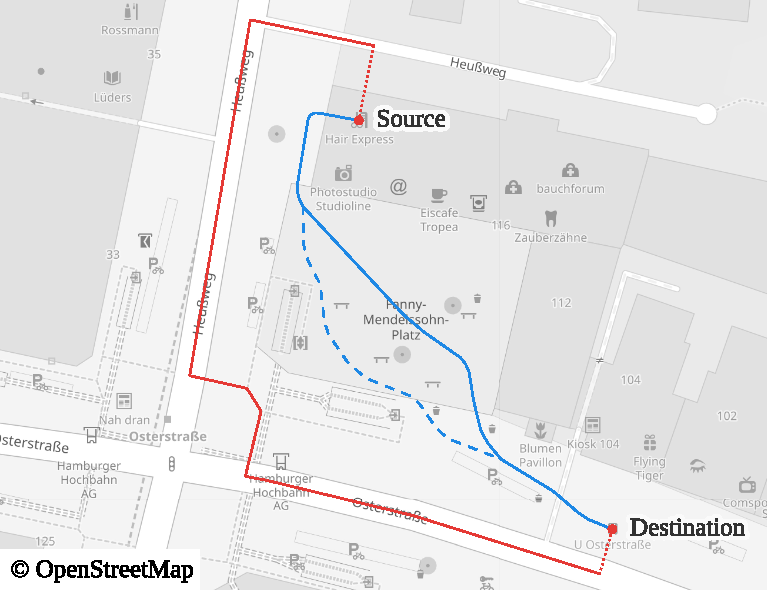
\includegraphics[width=\textwidth]{images/qgis-routing-osterstrasse-expected-vs-routing}
						\end{figcenter}
						\caption{The graph-based routing result (red) and the expected route (blue). The red dotted parts are direct connections to the closest point on an edge.}
						\label{fig:eval-osterstrasse-route-expected}
					\end{subfigure}
				\end{minipage}
				\hfill
				\begin{minipage}[t]{.48\textwidth}
					\begin{subfigure}[t]{\linewidth}
						\begin{figcenter}
							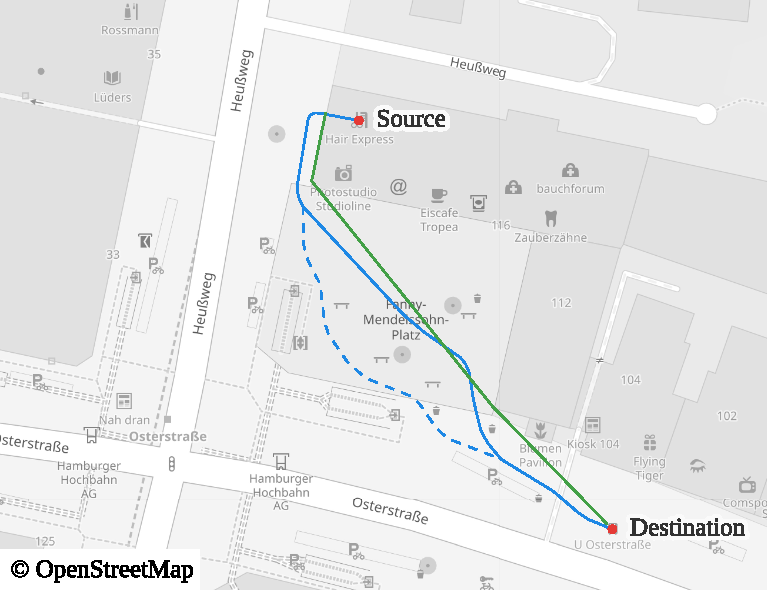
\includegraphics[width=\textwidth]{images/qgis-routing-osterstrasse-expected-vs-actual}
						\end{figcenter}
						\caption{The result of the hybrid routing algorithm (green) and the expected route (blue).}
						\label{fig:eval-osterstrasse-actual-expected}
					\end{subfigure}
				\end{minipage}
				\caption{Comparison of a graph-based route (red; determined on \href{https://www.openstreetmap.org/directions?engine=fossgis\_osrm\_foot\&route=53.57657\%2C9.95210\%3B53.57601\%2C9.95268\#map=19/53.57632/9.95218}{osm.org}) with the hybrid routing algorithm (green) and the expected result (blue). The dashed part of the expected result is an equally good alternative route. The difficulty of this scenario is the traversal of the square \enquote{Fanny-Mendelssohn Platz}.}
				\label{fig:eval-osterstrasse}
			\end{figure}
			
			% Interesting passages from the city dataset
			Next to the above example and comparison to graph-based routing, an analysis of the routes determined within the 1km\textsuperscript{2} \enquote{OSM city} dataset yields some noteworthy findings.
			
			First, the quality of a route significantly decreases with missing or wrong data as visible in \Cref{fig:eval-city-usefulness-b} and \ref{fig:eval-city-usefulness-c}.
			The passages marked in red in these images are often shortcuts via private property.
			Those areas, however, are usually filled with obstacles such as fences, walls or different kinds of vegetation.
			As described in \Cref{subsubsec:data-not-in-osm}, private areas in OSM often contain very few to no details.
			
			Second, within densely built-up areas, larger open spaces are rare and the combination of roads and buildings form corrdidors in which routes tend to lie.
			When and how often the route determined by the hybrid routing algorithm follows a road depends on the weighting function.
			
			\clearpage
			\begin{figure}[h!]
				\begin{minipage}[t]{.48\textwidth}
					\begin{subfigure}[t]{\linewidth}
						\begin{figcenter}
							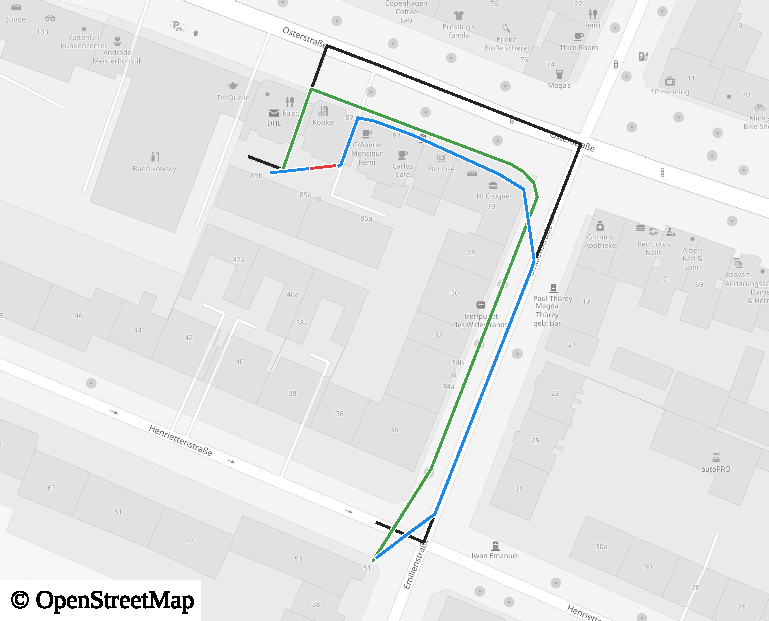
\includegraphics[width=\textwidth]{images/qgis-routing-city-routing-1}
						\end{figcenter}
						\caption{Simple route with only one small passage of missing data.}
						\label{fig:eval-city-usefulness-1}
					\end{subfigure}
				\end{minipage}
				\hfill
				\begin{minipage}[t]{.48\textwidth}
					\begin{subfigure}[t]{\linewidth}
						\begin{figcenter}
							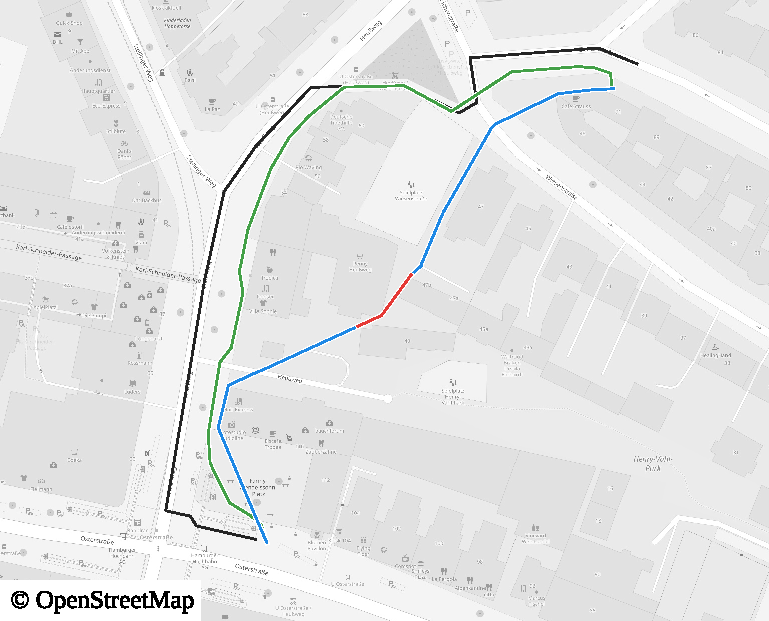
\includegraphics[width=\textwidth]{images/qgis-routing-city-routing-3}
						\end{figcenter}
						\caption{Missing obstacles (mainly walls and fences between buildings) lead to non-realistic routes.}
						\label{fig:eval-city-usefulness-b}
					\end{subfigure}
				\end{minipage}
				\\[3ex]
				\begin{minipage}[t]{.48\textwidth}
					\begin{subfigure}[t]{\linewidth}
						\begin{figcenter}
							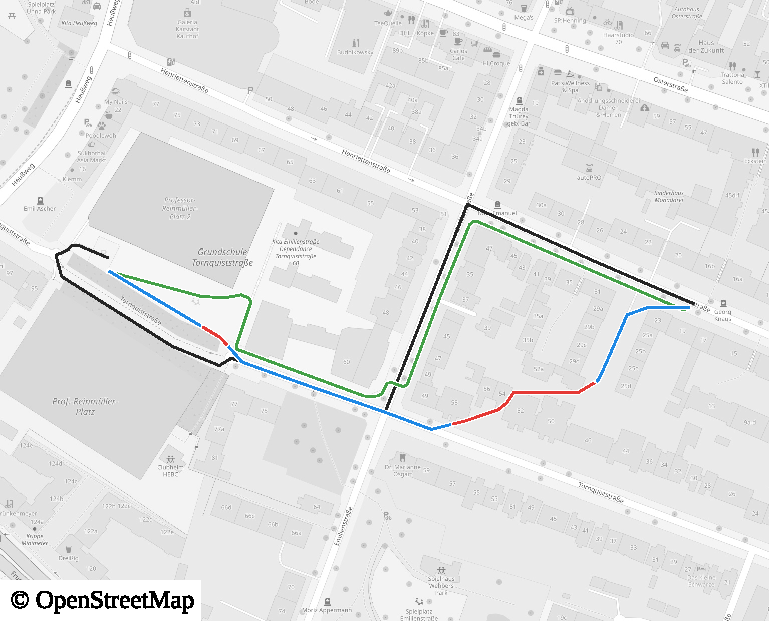
\includegraphics[width=\textwidth]{images/qgis-routing-city-routing-6}
						\end{figcenter}
						\caption{Missing walls, fences and hedges on private property are a common type of missing obstacles.}
						\label{fig:eval-city-usefulness-c}
					\end{subfigure}
				\end{minipage}
				\hfill
				\begin{minipage}[t]{.48\textwidth}
					\begin{subfigure}[t]{\linewidth}
						\begin{figcenter}
							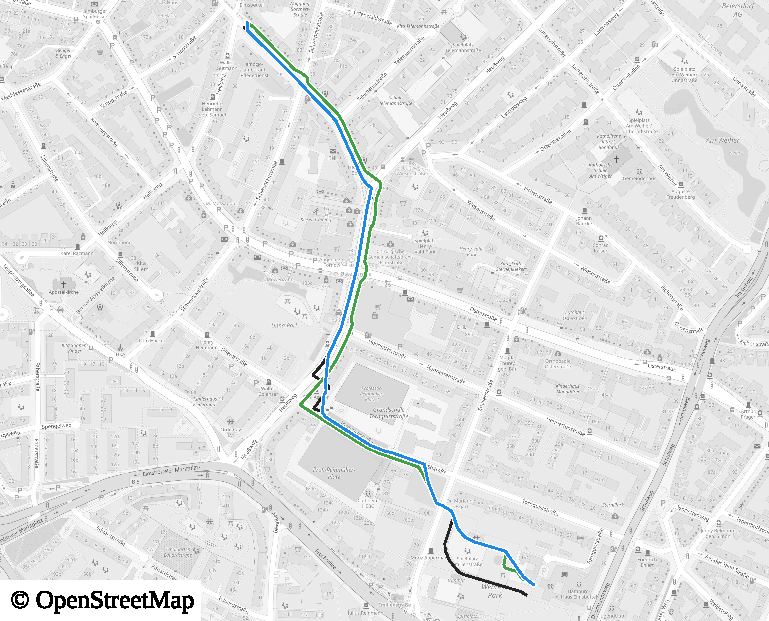
\includegraphics[width=\textwidth]{images/qgis-routing-city-routing-18}
						\end{figcenter}
						\caption{Cities with closed rows of buildings do not provide many degrees of freedom, which results in similar or even equal routes, regardles of the algorithm.}
						\label{fig:eval-city-usefulness-d}
					\end{subfigure}
				\end{minipage}
				\caption{Expected (green), graph-based (black) and hybrid routing algorithm results (blue) using the 1km\textsuperscript{2} city dataset. Unexpected parts due to missing or faulty data are marked in red.}
				\label{fig:eval-city-usefulness}
				\begin{minipage}[t]{.48\textwidth}
					\begin{figcenter}
						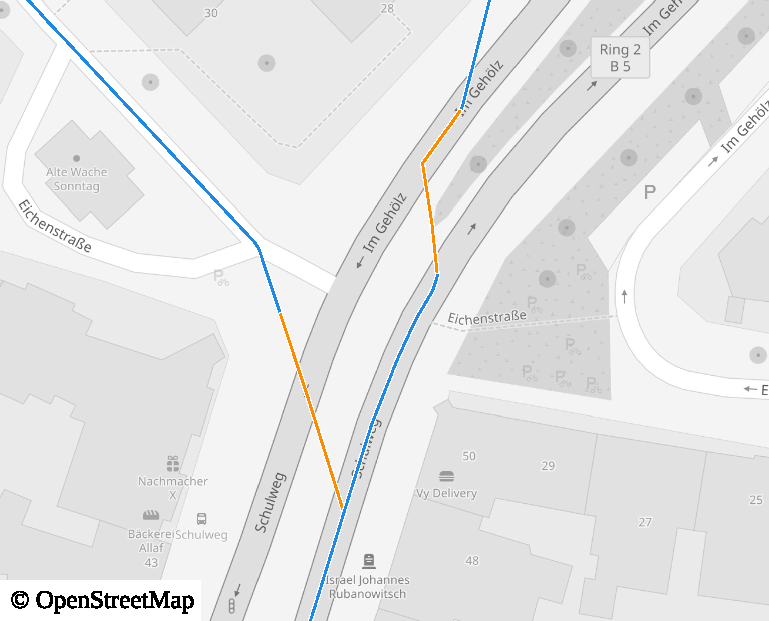
\includegraphics[width=\textwidth]{images/qgis-routing-city-roads}
					\end{figcenter}
					\caption{Two unrealistic road crossings (yellow) across a six-lane road.}
					\label{fig:eval-city-road-crossing}
				\end{minipage}
				\hfill
				\begin{minipage}[t]{.48\textwidth}
					\begin{figcenter}
						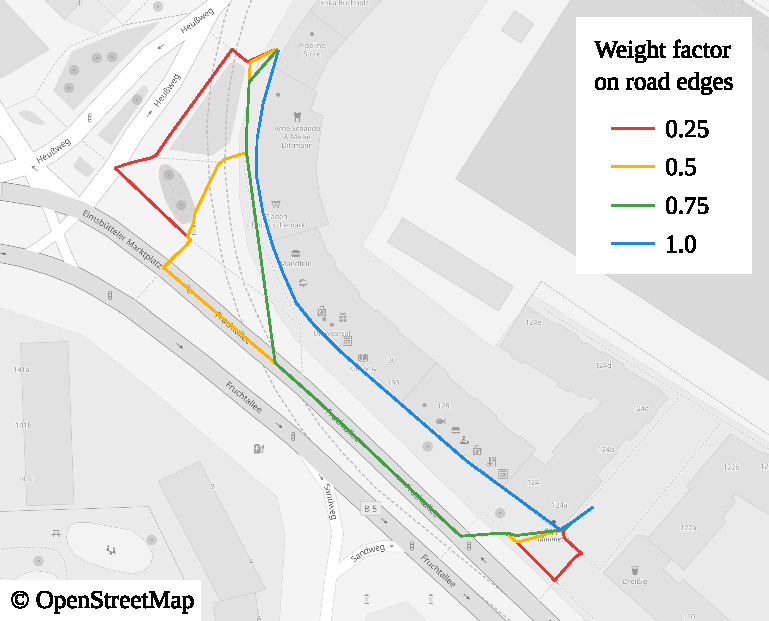
\includegraphics[width=\textwidth]{images/qgis-routing-city-weights}
					\end{figcenter}
					\caption{Influence of weight factors. Lower value result in a stronger preference for roads.}
					\label{fig:eval-city-weights}
				\end{minipage}
			\end{figure}
			
			Third, large roads create instances of the aforementioned rare but wide obstacle-free areas, which, however, might result in unrealistic road crossings.
			Such situation can be seen in \Cref{fig:eval-city-road-crossing} with crossings over a six-lane road, which would be dangerous and unrealistic for real-world pedestrians.
			
			Forth, the weight function has a huge impact on the route quality.
			It specifies for example how strongly roads should be preferred, which is illustrated in \Cref{fig:eval-city-weights} with the same route using different weights for road edges.
			Adjusting and definiting fine-grained weight functions may help to imporove the routing behavior in some of the above mentioned situations.
			
			% Interesting passages from the rural dataset
			In the \enquote{OSM city} datasets with only smaller open areas, graph-based routes and routes determined by the hybrid routing algorithm were often similar and some parts even identical.
			Datasets with larger open areas and irregular distributed obstacles, as in the \enquote{OSM rural} datasets, can greatly benefit from the hybrid routing algorithm.
			
			Figures \Cref{fig:eval-rural-routing-6} and \ref{fig:eval-rural-graph-based-comparison} give some examples on routes in a rural area with large open spaces.
			Two findings can be inferred from the analysis of the rural routing results.
			
			First, the difference between graph-based routes and routes from the hybrid routing algorithm is significantly larger.
			In fact, routes might not share any location and graph-based routes tend to be significantly longer.
			This can be seen in \Cref{fig:eval-rural-graph-based-comparison-6} with a graph-based route of 1.73km while the expected result is only 0.67km long.
			\Cref{fig:eval-rural-graph-based-comparison-17} shows a similar behavior even though the difference in distance is smaller because the graph-based, expected and actual route share common parts.
			
			Second, the accuracy and therefore the usefulness for real-world applications (such as navigation apps) heavily relies on the amount of details in the dataset.
			\Cref{fig:eval-rural-routing-6-osm} illustrates the problem of missing data, which are in this case missing ditches within the farmland.
			The determined route has a length of 365m while the shortest possible route (determined using aerial imagery as seen in \Cref{fig:eval-rural-routing-6-aerial}) is 677m long.
			
			\begin{figure}[h!]
				\begin{minipage}[t]{.48\textwidth}
					\begin{subfigure}[t]{\linewidth}
						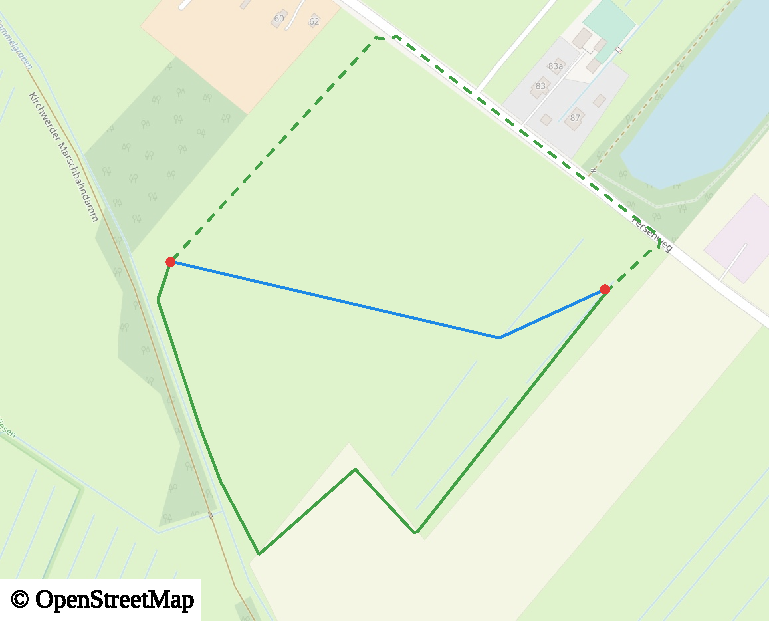
\includegraphics[width=\textwidth]{images/qgis-routing-rural-routing-6-osm}
						\caption{The expected route differs significantly from the actual route taken by the agent. The dashed line is an alternative route under the assumption, that the farmland is reachable from the upper road.}
						\label{fig:eval-rural-routing-6-osm}
					\end{subfigure}
				\end{minipage}
				\hfill
				\begin{minipage}[t]{.48\textwidth}
					\begin{subfigure}[t]{\linewidth}
						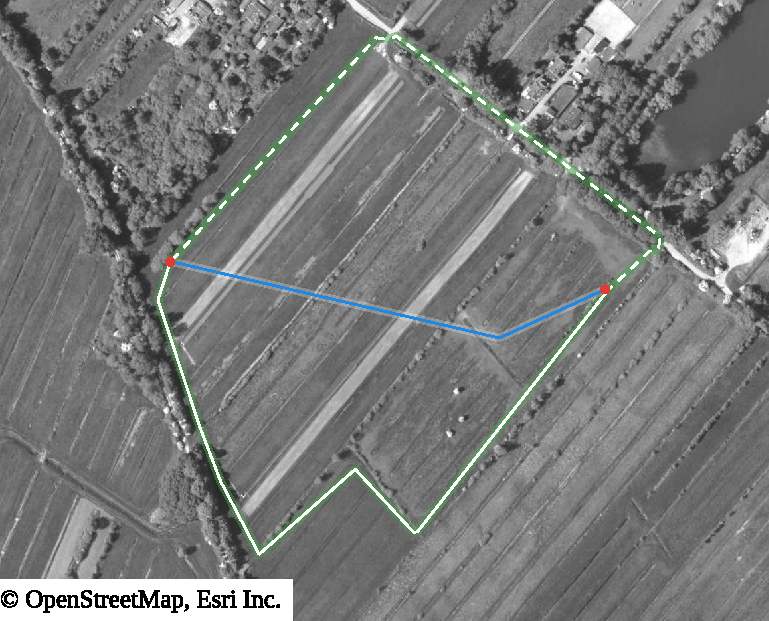
\includegraphics[width=\textwidth]{images/qgis-routing-rural-routing-6-aerial}
						\caption{Aerial imagery shows the amount of missing data, which in this case are numerous missing ditches in the arable land.}
						\label{fig:eval-rural-routing-6-aerial}
					\end{subfigure}
				\end{minipage}
				\caption{Routing on farmland illustrating the importance of correct data in the routing result showing the expected route (green) and actual path determined by the hybrid routing algorithm (green).}
				\label{fig:eval-rural-routing-6}
			\end{figure}
			
			\begin{figure}[h!]
				\begin{minipage}[t]{.48\textwidth}
					\begin{subfigure}[t]{\linewidth}
						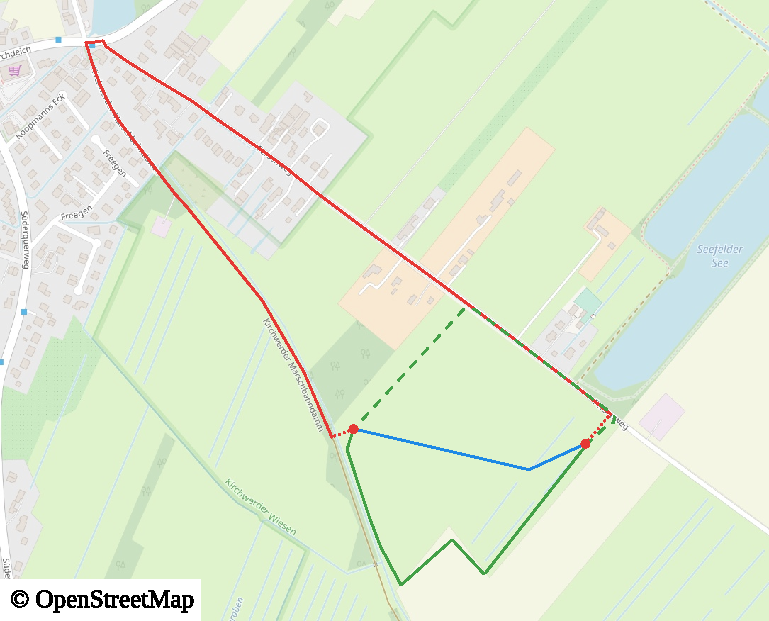
\includegraphics[width=\textwidth]{images/qgis-routing-rural-routing-6-graph-based}
						\caption{Same waypoints from \Cref{fig:eval-rural-routing-6} with the additional result of a graph-based routing request creating a 2.6 times longer path.}
						\label{fig:eval-rural-graph-based-comparison-6}
					\end{subfigure}
				\end{minipage}
				\hfill
				\begin{minipage}[t]{.48\textwidth}
					\begin{subfigure}[t]{\linewidth}
						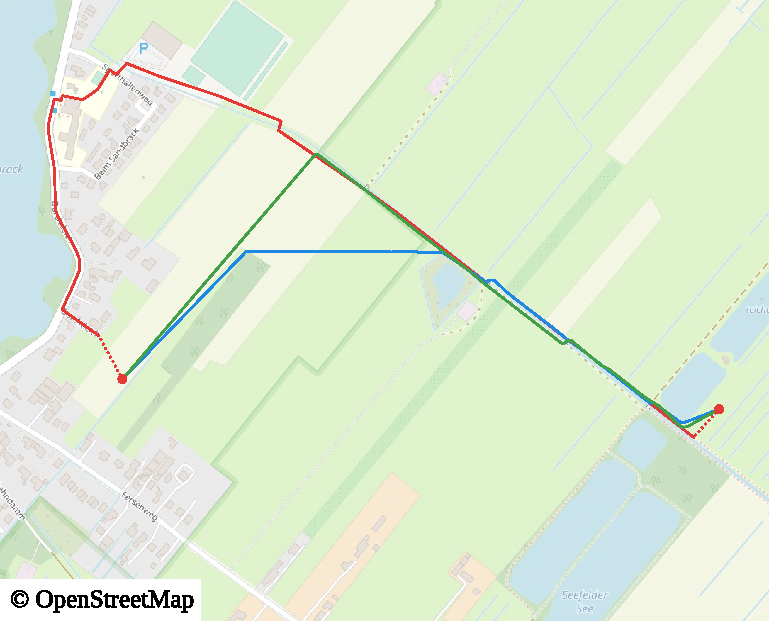
\includegraphics[width=\textwidth]{images/qgis-routing-rural-routing-17-graph-based}
						\caption{Example of detours created by a graph-based routing algorithm even though the first part of the result is equal to the one of the hybrid routing algorithm. The shortcut of the actual result (horizontal part of the blue route) is a result of missing obstacles similar to the situation visible in \Cref{fig:eval-rural-routing-6-aerial}.}
						\label{fig:eval-rural-graph-based-comparison-17}
					\end{subfigure}
				\end{minipage}
				\caption{Comparison of graph-based routing results (red) with the expected route (green) and actual results (blue) of the hybrid routing algorithm.}
				\label{fig:eval-rural-graph-based-comparison}
			\end{figure}
		
		\subsubsection{Mathematical route quality analysis}
		
			After a manual analysis of the route quality, mathematical approaches were used to obtain quantifiable results, which was done using two metrics.
			First, the beeline distance between two waypoints was compared to the distances of the corresponding expected route, the route based on the hybrid visibility graph and the route of graph-based routing.
			Second, the similarity of routes was determined to determine how well the results fit to the expected route
			Both comparisons were performed on the first ten routing requests of the OSM datasets.
			
			\begin{wrapfigure}{r}{0.35\textwidth}
				\vspace{-1\baselineskip}
				\begin{figcenter}
					\begin{tikzpicture}
					[
						every node/.append style={outer sep=0.5mm, inner sep=0}
					]
						\def\d{0.75}
						
						\node (c00) at (0.5*\d ,0) {};
						\node (c01) at (1*\d   ,1*\d) {};
						\node (c02) at (0.15*\d ,2*\d) {};
						\node (c03) at (0.55*\d,3*\d) {};
						\node (c04) at (0      ,4*\d) {};
						
						\node (c10) at (2*\d  ,0.15) {};
						\node (c11) at (2.1*\d,0.9*\d) {};
						\node (c12) at (1.25*\d,1.8*\d) {};
						\node (c13) at (3*\d  ,2.8*\d) {};
						\node (c14) at (1.2*\d,4.15*\d) {};
						
						\draw (c00.center) -- (c01.center) -- (c02.center) -- (c03.center) -- (c04.center);
						\draw (c10.center) -- (c11.center) -- (c12.center) -- (c13.center) -- (c14.center);
						
						\draw[>=stealth',<->,densely dotted] (c00) -- (c10);
						\draw[>=stealth',<->,densely dotted] (c01) -- (c11);
						\draw[>=stealth',<->,densely dotted] (c02) -- (c12);
						\draw[>=stealth',<->,thick,red] (c03) -- (c13);
						\draw[>=stealth',<->,densely dotted] (c04) -- (c14);
						
						% Enlarge BBOX to avoid cropping off some of the arrow heads:
						\node (bbox_a) at (-0.1,-0.1) {};
						\node (bbox_b) at (3*\d+0.1,4.15*\d+0.1) {};
					\end{tikzpicture}
				\end{figcenter}
				\caption{Hausdorff distance (red) between two linestrings.}
				\label{fig:hausdorff-distance}
			\end{wrapfigure}
			
			In \Cref{fig:eval-route-distances}, the distance factors show an important relation between the route distances.
			The mean value of both datasets indicate, that the average route from the hybrid routing algorithm is shorter and the average route of the graph-based routing is longer than the expected route.
			This is in line with the results of the previous manual route analysis, according to which missing data lead to unrealistic but shorter routes.
			The route length comparison also confirms the previous results, that graph-based routing leads to longer routes with sometimes significant detours, which can be seen in the routing requests 6 and 7 in \Cref{fig:eval-route-distances-rural}.
			
			\begin{figure}[h]
				\begin{subfigure}[t]{\linewidth}
					\begin{figcenter}
						%% Creator: Matplotlib, PGF backend
%%
%% To include the figure in your LaTeX document, write
%%   \input{<filename>.pgf}
%%
%% Make sure the required packages are loaded in your preamble
%%   \usepackage{pgf}
%%
%% Also ensure that all the required font packages are loaded; for instance,
%% the lmodern package is sometimes necessary when using math font.
%%   \usepackage{lmodern}
%%
%% Figures using additional raster images can only be included by \input if
%% they are in the same directory as the main LaTeX file. For loading figures
%% from other directories you can use the `import` package
%%   \usepackage{import}
%%
%% and then include the figures with
%%   \import{<path to file>}{<filename>.pgf}
%%
%% Matplotlib used the following preamble
%%   
%%   \usepackage{fontspec}
%%   \setmainfont{DejaVuSerif.ttf}[Path=\detokenize{/home/hauke/.local/lib/python3.11/site-packages/matplotlib/mpl-data/fonts/ttf/}]
%%   \setsansfont{DroidSans.ttf}[Path=\detokenize{/usr/share/fonts/droid/}]
%%   \setmonofont{DejaVuSansMono.ttf}[Path=\detokenize{/home/hauke/.local/lib/python3.11/site-packages/matplotlib/mpl-data/fonts/ttf/}]
%%   \makeatletter\@ifpackageloaded{underscore}{}{\usepackage[strings]{underscore}}\makeatother
%%
\begingroup%
\makeatletter%
\begin{pgfpicture}%
\pgfpathrectangle{\pgfpointorigin}{\pgfqpoint{6.086410in}{1.715788in}}%
\pgfusepath{use as bounding box, clip}%
\begin{pgfscope}%
\pgfsetbuttcap%
\pgfsetmiterjoin%
\definecolor{currentfill}{rgb}{1.000000,1.000000,1.000000}%
\pgfsetfillcolor{currentfill}%
\pgfsetlinewidth{0.000000pt}%
\definecolor{currentstroke}{rgb}{1.000000,1.000000,1.000000}%
\pgfsetstrokecolor{currentstroke}%
\pgfsetdash{}{0pt}%
\pgfpathmoveto{\pgfqpoint{0.000000in}{0.000000in}}%
\pgfpathlineto{\pgfqpoint{6.086410in}{0.000000in}}%
\pgfpathlineto{\pgfqpoint{6.086410in}{1.715788in}}%
\pgfpathlineto{\pgfqpoint{0.000000in}{1.715788in}}%
\pgfpathlineto{\pgfqpoint{0.000000in}{0.000000in}}%
\pgfpathclose%
\pgfusepath{fill}%
\end{pgfscope}%
\begin{pgfscope}%
\pgfsetbuttcap%
\pgfsetmiterjoin%
\definecolor{currentfill}{rgb}{1.000000,1.000000,1.000000}%
\pgfsetfillcolor{currentfill}%
\pgfsetlinewidth{0.000000pt}%
\definecolor{currentstroke}{rgb}{0.000000,0.000000,0.000000}%
\pgfsetstrokecolor{currentstroke}%
\pgfsetstrokeopacity{0.000000}%
\pgfsetdash{}{0pt}%
\pgfpathmoveto{\pgfqpoint{0.641586in}{0.451389in}}%
\pgfpathlineto{\pgfqpoint{4.921145in}{0.451389in}}%
\pgfpathlineto{\pgfqpoint{4.921145in}{1.715788in}}%
\pgfpathlineto{\pgfqpoint{0.641586in}{1.715788in}}%
\pgfpathlineto{\pgfqpoint{0.641586in}{0.451389in}}%
\pgfpathclose%
\pgfusepath{fill}%
\end{pgfscope}%
\begin{pgfscope}%
\definecolor{textcolor}{rgb}{0.150000,0.150000,0.150000}%
\pgfsetstrokecolor{textcolor}%
\pgfsetfillcolor{textcolor}%
\pgftext[x=0.836112in,y=0.319444in,,top]{\color{textcolor}\sffamily\fontsize{9.000000}{10.800000}\selectfont 1}%
\end{pgfscope}%
\begin{pgfscope}%
\definecolor{textcolor}{rgb}{0.150000,0.150000,0.150000}%
\pgfsetstrokecolor{textcolor}%
\pgfsetfillcolor{textcolor}%
\pgftext[x=1.225163in,y=0.319444in,,top]{\color{textcolor}\sffamily\fontsize{9.000000}{10.800000}\selectfont 2}%
\end{pgfscope}%
\begin{pgfscope}%
\definecolor{textcolor}{rgb}{0.150000,0.150000,0.150000}%
\pgfsetstrokecolor{textcolor}%
\pgfsetfillcolor{textcolor}%
\pgftext[x=1.614213in,y=0.319444in,,top]{\color{textcolor}\sffamily\fontsize{9.000000}{10.800000}\selectfont 3}%
\end{pgfscope}%
\begin{pgfscope}%
\definecolor{textcolor}{rgb}{0.150000,0.150000,0.150000}%
\pgfsetstrokecolor{textcolor}%
\pgfsetfillcolor{textcolor}%
\pgftext[x=2.003264in,y=0.319444in,,top]{\color{textcolor}\sffamily\fontsize{9.000000}{10.800000}\selectfont 4}%
\end{pgfscope}%
\begin{pgfscope}%
\definecolor{textcolor}{rgb}{0.150000,0.150000,0.150000}%
\pgfsetstrokecolor{textcolor}%
\pgfsetfillcolor{textcolor}%
\pgftext[x=2.392315in,y=0.319444in,,top]{\color{textcolor}\sffamily\fontsize{9.000000}{10.800000}\selectfont 5}%
\end{pgfscope}%
\begin{pgfscope}%
\definecolor{textcolor}{rgb}{0.150000,0.150000,0.150000}%
\pgfsetstrokecolor{textcolor}%
\pgfsetfillcolor{textcolor}%
\pgftext[x=2.781366in,y=0.319444in,,top]{\color{textcolor}\sffamily\fontsize{9.000000}{10.800000}\selectfont 6}%
\end{pgfscope}%
\begin{pgfscope}%
\definecolor{textcolor}{rgb}{0.150000,0.150000,0.150000}%
\pgfsetstrokecolor{textcolor}%
\pgfsetfillcolor{textcolor}%
\pgftext[x=3.170416in,y=0.319444in,,top]{\color{textcolor}\sffamily\fontsize{9.000000}{10.800000}\selectfont 7}%
\end{pgfscope}%
\begin{pgfscope}%
\definecolor{textcolor}{rgb}{0.150000,0.150000,0.150000}%
\pgfsetstrokecolor{textcolor}%
\pgfsetfillcolor{textcolor}%
\pgftext[x=3.559467in,y=0.319444in,,top]{\color{textcolor}\sffamily\fontsize{9.000000}{10.800000}\selectfont 8}%
\end{pgfscope}%
\begin{pgfscope}%
\definecolor{textcolor}{rgb}{0.150000,0.150000,0.150000}%
\pgfsetstrokecolor{textcolor}%
\pgfsetfillcolor{textcolor}%
\pgftext[x=3.948518in,y=0.319444in,,top]{\color{textcolor}\sffamily\fontsize{9.000000}{10.800000}\selectfont 9}%
\end{pgfscope}%
\begin{pgfscope}%
\definecolor{textcolor}{rgb}{0.150000,0.150000,0.150000}%
\pgfsetstrokecolor{textcolor}%
\pgfsetfillcolor{textcolor}%
\pgftext[x=4.337569in,y=0.319444in,,top]{\color{textcolor}\sffamily\fontsize{9.000000}{10.800000}\selectfont 10}%
\end{pgfscope}%
\begin{pgfscope}%
\definecolor{textcolor}{rgb}{0.150000,0.150000,0.150000}%
\pgfsetstrokecolor{textcolor}%
\pgfsetfillcolor{textcolor}%
\pgftext[x=4.726620in,y=0.319444in,,top]{\color{textcolor}\sffamily\fontsize{9.000000}{10.800000}\selectfont mean}%
\end{pgfscope}%
\begin{pgfscope}%
\definecolor{textcolor}{rgb}{0.150000,0.150000,0.150000}%
\pgfsetstrokecolor{textcolor}%
\pgfsetfillcolor{textcolor}%
\pgftext[x=2.781366in,y=0.125000in,,top]{\color{textcolor}\sffamily\fontsize{9.000000}{10.800000}\selectfont Routing request}%
\end{pgfscope}%
\begin{pgfscope}%
\pgfpathrectangle{\pgfqpoint{0.641586in}{0.451389in}}{\pgfqpoint{4.279559in}{1.264399in}}%
\pgfusepath{clip}%
\pgfsetroundcap%
\pgfsetroundjoin%
\pgfsetlinewidth{1.003750pt}%
\definecolor{currentstroke}{rgb}{0.800000,0.800000,0.800000}%
\pgfsetstrokecolor{currentstroke}%
\pgfsetdash{}{0pt}%
\pgfpathmoveto{\pgfqpoint{0.641586in}{0.537753in}}%
\pgfpathlineto{\pgfqpoint{4.921145in}{0.537753in}}%
\pgfusepath{stroke}%
\end{pgfscope}%
\begin{pgfscope}%
\definecolor{textcolor}{rgb}{0.150000,0.150000,0.150000}%
\pgfsetstrokecolor{textcolor}%
\pgfsetfillcolor{textcolor}%
\pgftext[x=0.338438in, y=0.490267in, left, base]{\color{textcolor}\sffamily\fontsize{9.000000}{10.800000}\selectfont 1.0}%
\end{pgfscope}%
\begin{pgfscope}%
\pgfpathrectangle{\pgfqpoint{0.641586in}{0.451389in}}{\pgfqpoint{4.279559in}{1.264399in}}%
\pgfusepath{clip}%
\pgfsetroundcap%
\pgfsetroundjoin%
\pgfsetlinewidth{1.003750pt}%
\definecolor{currentstroke}{rgb}{0.800000,0.800000,0.800000}%
\pgfsetstrokecolor{currentstroke}%
\pgfsetdash{}{0pt}%
\pgfpathmoveto{\pgfqpoint{0.641586in}{0.969573in}}%
\pgfpathlineto{\pgfqpoint{4.921145in}{0.969573in}}%
\pgfusepath{stroke}%
\end{pgfscope}%
\begin{pgfscope}%
\definecolor{textcolor}{rgb}{0.150000,0.150000,0.150000}%
\pgfsetstrokecolor{textcolor}%
\pgfsetfillcolor{textcolor}%
\pgftext[x=0.338438in, y=0.922088in, left, base]{\color{textcolor}\sffamily\fontsize{9.000000}{10.800000}\selectfont 1.5}%
\end{pgfscope}%
\begin{pgfscope}%
\pgfpathrectangle{\pgfqpoint{0.641586in}{0.451389in}}{\pgfqpoint{4.279559in}{1.264399in}}%
\pgfusepath{clip}%
\pgfsetroundcap%
\pgfsetroundjoin%
\pgfsetlinewidth{1.003750pt}%
\definecolor{currentstroke}{rgb}{0.800000,0.800000,0.800000}%
\pgfsetstrokecolor{currentstroke}%
\pgfsetdash{}{0pt}%
\pgfpathmoveto{\pgfqpoint{0.641586in}{1.401393in}}%
\pgfpathlineto{\pgfqpoint{4.921145in}{1.401393in}}%
\pgfusepath{stroke}%
\end{pgfscope}%
\begin{pgfscope}%
\definecolor{textcolor}{rgb}{0.150000,0.150000,0.150000}%
\pgfsetstrokecolor{textcolor}%
\pgfsetfillcolor{textcolor}%
\pgftext[x=0.338438in, y=1.353908in, left, base]{\color{textcolor}\sffamily\fontsize{9.000000}{10.800000}\selectfont 2.0}%
\end{pgfscope}%
\begin{pgfscope}%
\definecolor{textcolor}{rgb}{0.150000,0.150000,0.150000}%
\pgfsetstrokecolor{textcolor}%
\pgfsetfillcolor{textcolor}%
\pgftext[x=0.094971in, y=0.628907in, left, base,rotate=90.000000]{\color{textcolor}\sffamily\fontsize{9.000000}{10.800000}\selectfont Route distance /}%
\end{pgfscope}%
\begin{pgfscope}%
\definecolor{textcolor}{rgb}{0.150000,0.150000,0.150000}%
\pgfsetstrokecolor{textcolor}%
\pgfsetfillcolor{textcolor}%
\pgftext[x=0.238965in, y=0.626709in, left, base,rotate=90.000000]{\color{textcolor}\sffamily\fontsize{9.000000}{10.800000}\selectfont beeline distance}%
\end{pgfscope}%
\begin{pgfscope}%
\pgfpathrectangle{\pgfqpoint{0.641586in}{0.451389in}}{\pgfqpoint{4.279559in}{1.264399in}}%
\pgfusepath{clip}%
\pgfsetbuttcap%
\pgfsetmiterjoin%
\definecolor{currentfill}{rgb}{0.460784,0.749020,0.443137}%
\pgfsetfillcolor{currentfill}%
\pgfsetlinewidth{1.003750pt}%
\definecolor{currentstroke}{rgb}{1.000000,1.000000,1.000000}%
\pgfsetstrokecolor{currentstroke}%
\pgfsetdash{}{0pt}%
\pgfpathmoveto{\pgfqpoint{0.680491in}{-0.325888in}}%
\pgfpathlineto{\pgfqpoint{0.784238in}{-0.325888in}}%
\pgfpathlineto{\pgfqpoint{0.784238in}{1.307054in}}%
\pgfpathlineto{\pgfqpoint{0.680491in}{1.307054in}}%
\pgfpathlineto{\pgfqpoint{0.680491in}{-0.325888in}}%
\pgfpathclose%
\pgfusepath{stroke,fill}%
\end{pgfscope}%
\begin{pgfscope}%
\pgfpathrectangle{\pgfqpoint{0.641586in}{0.451389in}}{\pgfqpoint{4.279559in}{1.264399in}}%
\pgfusepath{clip}%
\pgfsetbuttcap%
\pgfsetmiterjoin%
\definecolor{currentfill}{rgb}{0.460784,0.749020,0.443137}%
\pgfsetfillcolor{currentfill}%
\pgfsetlinewidth{1.003750pt}%
\definecolor{currentstroke}{rgb}{1.000000,1.000000,1.000000}%
\pgfsetstrokecolor{currentstroke}%
\pgfsetdash{}{0pt}%
\pgfpathmoveto{\pgfqpoint{1.069542in}{-0.325888in}}%
\pgfpathlineto{\pgfqpoint{1.173289in}{-0.325888in}}%
\pgfpathlineto{\pgfqpoint{1.173289in}{0.742690in}}%
\pgfpathlineto{\pgfqpoint{1.069542in}{0.742690in}}%
\pgfpathlineto{\pgfqpoint{1.069542in}{-0.325888in}}%
\pgfpathclose%
\pgfusepath{stroke,fill}%
\end{pgfscope}%
\begin{pgfscope}%
\pgfpathrectangle{\pgfqpoint{0.641586in}{0.451389in}}{\pgfqpoint{4.279559in}{1.264399in}}%
\pgfusepath{clip}%
\pgfsetbuttcap%
\pgfsetmiterjoin%
\definecolor{currentfill}{rgb}{0.460784,0.749020,0.443137}%
\pgfsetfillcolor{currentfill}%
\pgfsetlinewidth{1.003750pt}%
\definecolor{currentstroke}{rgb}{1.000000,1.000000,1.000000}%
\pgfsetstrokecolor{currentstroke}%
\pgfsetdash{}{0pt}%
\pgfpathmoveto{\pgfqpoint{1.458593in}{-0.325888in}}%
\pgfpathlineto{\pgfqpoint{1.562340in}{-0.325888in}}%
\pgfpathlineto{\pgfqpoint{1.562340in}{0.919651in}}%
\pgfpathlineto{\pgfqpoint{1.458593in}{0.919651in}}%
\pgfpathlineto{\pgfqpoint{1.458593in}{-0.325888in}}%
\pgfpathclose%
\pgfusepath{stroke,fill}%
\end{pgfscope}%
\begin{pgfscope}%
\pgfpathrectangle{\pgfqpoint{0.641586in}{0.451389in}}{\pgfqpoint{4.279559in}{1.264399in}}%
\pgfusepath{clip}%
\pgfsetbuttcap%
\pgfsetmiterjoin%
\definecolor{currentfill}{rgb}{0.460784,0.749020,0.443137}%
\pgfsetfillcolor{currentfill}%
\pgfsetlinewidth{1.003750pt}%
\definecolor{currentstroke}{rgb}{1.000000,1.000000,1.000000}%
\pgfsetstrokecolor{currentstroke}%
\pgfsetdash{}{0pt}%
\pgfpathmoveto{\pgfqpoint{1.847644in}{-0.325888in}}%
\pgfpathlineto{\pgfqpoint{1.951391in}{-0.325888in}}%
\pgfpathlineto{\pgfqpoint{1.951391in}{0.553689in}}%
\pgfpathlineto{\pgfqpoint{1.847644in}{0.553689in}}%
\pgfpathlineto{\pgfqpoint{1.847644in}{-0.325888in}}%
\pgfpathclose%
\pgfusepath{stroke,fill}%
\end{pgfscope}%
\begin{pgfscope}%
\pgfpathrectangle{\pgfqpoint{0.641586in}{0.451389in}}{\pgfqpoint{4.279559in}{1.264399in}}%
\pgfusepath{clip}%
\pgfsetbuttcap%
\pgfsetmiterjoin%
\definecolor{currentfill}{rgb}{0.460784,0.749020,0.443137}%
\pgfsetfillcolor{currentfill}%
\pgfsetlinewidth{1.003750pt}%
\definecolor{currentstroke}{rgb}{1.000000,1.000000,1.000000}%
\pgfsetstrokecolor{currentstroke}%
\pgfsetdash{}{0pt}%
\pgfpathmoveto{\pgfqpoint{2.236695in}{-0.325888in}}%
\pgfpathlineto{\pgfqpoint{2.340441in}{-0.325888in}}%
\pgfpathlineto{\pgfqpoint{2.340441in}{1.254489in}}%
\pgfpathlineto{\pgfqpoint{2.236695in}{1.254489in}}%
\pgfpathlineto{\pgfqpoint{2.236695in}{-0.325888in}}%
\pgfpathclose%
\pgfusepath{stroke,fill}%
\end{pgfscope}%
\begin{pgfscope}%
\pgfpathrectangle{\pgfqpoint{0.641586in}{0.451389in}}{\pgfqpoint{4.279559in}{1.264399in}}%
\pgfusepath{clip}%
\pgfsetbuttcap%
\pgfsetmiterjoin%
\definecolor{currentfill}{rgb}{0.460784,0.749020,0.443137}%
\pgfsetfillcolor{currentfill}%
\pgfsetlinewidth{1.003750pt}%
\definecolor{currentstroke}{rgb}{1.000000,1.000000,1.000000}%
\pgfsetstrokecolor{currentstroke}%
\pgfsetdash{}{0pt}%
\pgfpathmoveto{\pgfqpoint{2.625745in}{-0.325888in}}%
\pgfpathlineto{\pgfqpoint{2.729492in}{-0.325888in}}%
\pgfpathlineto{\pgfqpoint{2.729492in}{0.860332in}}%
\pgfpathlineto{\pgfqpoint{2.625745in}{0.860332in}}%
\pgfpathlineto{\pgfqpoint{2.625745in}{-0.325888in}}%
\pgfpathclose%
\pgfusepath{stroke,fill}%
\end{pgfscope}%
\begin{pgfscope}%
\pgfpathrectangle{\pgfqpoint{0.641586in}{0.451389in}}{\pgfqpoint{4.279559in}{1.264399in}}%
\pgfusepath{clip}%
\pgfsetbuttcap%
\pgfsetmiterjoin%
\definecolor{currentfill}{rgb}{0.460784,0.749020,0.443137}%
\pgfsetfillcolor{currentfill}%
\pgfsetlinewidth{1.003750pt}%
\definecolor{currentstroke}{rgb}{1.000000,1.000000,1.000000}%
\pgfsetstrokecolor{currentstroke}%
\pgfsetdash{}{0pt}%
\pgfpathmoveto{\pgfqpoint{3.014796in}{-0.325888in}}%
\pgfpathlineto{\pgfqpoint{3.118543in}{-0.325888in}}%
\pgfpathlineto{\pgfqpoint{3.118543in}{0.930075in}}%
\pgfpathlineto{\pgfqpoint{3.014796in}{0.930075in}}%
\pgfpathlineto{\pgfqpoint{3.014796in}{-0.325888in}}%
\pgfpathclose%
\pgfusepath{stroke,fill}%
\end{pgfscope}%
\begin{pgfscope}%
\pgfpathrectangle{\pgfqpoint{0.641586in}{0.451389in}}{\pgfqpoint{4.279559in}{1.264399in}}%
\pgfusepath{clip}%
\pgfsetbuttcap%
\pgfsetmiterjoin%
\definecolor{currentfill}{rgb}{0.460784,0.749020,0.443137}%
\pgfsetfillcolor{currentfill}%
\pgfsetlinewidth{1.003750pt}%
\definecolor{currentstroke}{rgb}{1.000000,1.000000,1.000000}%
\pgfsetstrokecolor{currentstroke}%
\pgfsetdash{}{0pt}%
\pgfpathmoveto{\pgfqpoint{3.403847in}{-0.325888in}}%
\pgfpathlineto{\pgfqpoint{3.507594in}{-0.325888in}}%
\pgfpathlineto{\pgfqpoint{3.507594in}{1.025255in}}%
\pgfpathlineto{\pgfqpoint{3.403847in}{1.025255in}}%
\pgfpathlineto{\pgfqpoint{3.403847in}{-0.325888in}}%
\pgfpathclose%
\pgfusepath{stroke,fill}%
\end{pgfscope}%
\begin{pgfscope}%
\pgfpathrectangle{\pgfqpoint{0.641586in}{0.451389in}}{\pgfqpoint{4.279559in}{1.264399in}}%
\pgfusepath{clip}%
\pgfsetbuttcap%
\pgfsetmiterjoin%
\definecolor{currentfill}{rgb}{0.460784,0.749020,0.443137}%
\pgfsetfillcolor{currentfill}%
\pgfsetlinewidth{1.003750pt}%
\definecolor{currentstroke}{rgb}{1.000000,1.000000,1.000000}%
\pgfsetstrokecolor{currentstroke}%
\pgfsetdash{}{0pt}%
\pgfpathmoveto{\pgfqpoint{3.792898in}{-0.325888in}}%
\pgfpathlineto{\pgfqpoint{3.896645in}{-0.325888in}}%
\pgfpathlineto{\pgfqpoint{3.896645in}{0.923694in}}%
\pgfpathlineto{\pgfqpoint{3.792898in}{0.923694in}}%
\pgfpathlineto{\pgfqpoint{3.792898in}{-0.325888in}}%
\pgfpathclose%
\pgfusepath{stroke,fill}%
\end{pgfscope}%
\begin{pgfscope}%
\pgfpathrectangle{\pgfqpoint{0.641586in}{0.451389in}}{\pgfqpoint{4.279559in}{1.264399in}}%
\pgfusepath{clip}%
\pgfsetbuttcap%
\pgfsetmiterjoin%
\definecolor{currentfill}{rgb}{0.460784,0.749020,0.443137}%
\pgfsetfillcolor{currentfill}%
\pgfsetlinewidth{1.003750pt}%
\definecolor{currentstroke}{rgb}{1.000000,1.000000,1.000000}%
\pgfsetstrokecolor{currentstroke}%
\pgfsetdash{}{0pt}%
\pgfpathmoveto{\pgfqpoint{4.181948in}{-0.325888in}}%
\pgfpathlineto{\pgfqpoint{4.285695in}{-0.325888in}}%
\pgfpathlineto{\pgfqpoint{4.285695in}{1.087734in}}%
\pgfpathlineto{\pgfqpoint{4.181948in}{1.087734in}}%
\pgfpathlineto{\pgfqpoint{4.181948in}{-0.325888in}}%
\pgfpathclose%
\pgfusepath{stroke,fill}%
\end{pgfscope}%
\begin{pgfscope}%
\pgfpathrectangle{\pgfqpoint{0.641586in}{0.451389in}}{\pgfqpoint{4.279559in}{1.264399in}}%
\pgfusepath{clip}%
\pgfsetbuttcap%
\pgfsetmiterjoin%
\definecolor{currentfill}{rgb}{0.460784,0.749020,0.443137}%
\pgfsetfillcolor{currentfill}%
\pgfsetlinewidth{1.003750pt}%
\definecolor{currentstroke}{rgb}{1.000000,1.000000,1.000000}%
\pgfsetstrokecolor{currentstroke}%
\pgfsetdash{}{0pt}%
\pgfpathmoveto{\pgfqpoint{4.570999in}{-0.325888in}}%
\pgfpathlineto{\pgfqpoint{4.674746in}{-0.325888in}}%
\pgfpathlineto{\pgfqpoint{4.674746in}{0.960466in}}%
\pgfpathlineto{\pgfqpoint{4.570999in}{0.960466in}}%
\pgfpathlineto{\pgfqpoint{4.570999in}{-0.325888in}}%
\pgfpathclose%
\pgfusepath{stroke,fill}%
\end{pgfscope}%
\begin{pgfscope}%
\pgfpathrectangle{\pgfqpoint{0.641586in}{0.451389in}}{\pgfqpoint{4.279559in}{1.264399in}}%
\pgfusepath{clip}%
\pgfsetbuttcap%
\pgfsetmiterjoin%
\definecolor{currentfill}{rgb}{0.349020,0.490196,0.749020}%
\pgfsetfillcolor{currentfill}%
\pgfsetlinewidth{1.003750pt}%
\definecolor{currentstroke}{rgb}{1.000000,1.000000,1.000000}%
\pgfsetstrokecolor{currentstroke}%
\pgfsetdash{}{0pt}%
\pgfpathmoveto{\pgfqpoint{0.784238in}{-0.325888in}}%
\pgfpathlineto{\pgfqpoint{0.887985in}{-0.325888in}}%
\pgfpathlineto{\pgfqpoint{0.887985in}{1.271194in}}%
\pgfpathlineto{\pgfqpoint{0.784238in}{1.271194in}}%
\pgfpathlineto{\pgfqpoint{0.784238in}{-0.325888in}}%
\pgfpathclose%
\pgfusepath{stroke,fill}%
\end{pgfscope}%
\begin{pgfscope}%
\pgfpathrectangle{\pgfqpoint{0.641586in}{0.451389in}}{\pgfqpoint{4.279559in}{1.264399in}}%
\pgfusepath{clip}%
\pgfsetbuttcap%
\pgfsetmiterjoin%
\definecolor{currentfill}{rgb}{0.349020,0.490196,0.749020}%
\pgfsetfillcolor{currentfill}%
\pgfsetlinewidth{1.003750pt}%
\definecolor{currentstroke}{rgb}{1.000000,1.000000,1.000000}%
\pgfsetstrokecolor{currentstroke}%
\pgfsetdash{}{0pt}%
\pgfpathmoveto{\pgfqpoint{1.173289in}{-0.325888in}}%
\pgfpathlineto{\pgfqpoint{1.277036in}{-0.325888in}}%
\pgfpathlineto{\pgfqpoint{1.277036in}{0.682497in}}%
\pgfpathlineto{\pgfqpoint{1.173289in}{0.682497in}}%
\pgfpathlineto{\pgfqpoint{1.173289in}{-0.325888in}}%
\pgfpathclose%
\pgfusepath{stroke,fill}%
\end{pgfscope}%
\begin{pgfscope}%
\pgfpathrectangle{\pgfqpoint{0.641586in}{0.451389in}}{\pgfqpoint{4.279559in}{1.264399in}}%
\pgfusepath{clip}%
\pgfsetbuttcap%
\pgfsetmiterjoin%
\definecolor{currentfill}{rgb}{0.349020,0.490196,0.749020}%
\pgfsetfillcolor{currentfill}%
\pgfsetlinewidth{1.003750pt}%
\definecolor{currentstroke}{rgb}{1.000000,1.000000,1.000000}%
\pgfsetstrokecolor{currentstroke}%
\pgfsetdash{}{0pt}%
\pgfpathmoveto{\pgfqpoint{1.562340in}{-0.325888in}}%
\pgfpathlineto{\pgfqpoint{1.666087in}{-0.325888in}}%
\pgfpathlineto{\pgfqpoint{1.666087in}{0.722822in}}%
\pgfpathlineto{\pgfqpoint{1.562340in}{0.722822in}}%
\pgfpathlineto{\pgfqpoint{1.562340in}{-0.325888in}}%
\pgfpathclose%
\pgfusepath{stroke,fill}%
\end{pgfscope}%
\begin{pgfscope}%
\pgfpathrectangle{\pgfqpoint{0.641586in}{0.451389in}}{\pgfqpoint{4.279559in}{1.264399in}}%
\pgfusepath{clip}%
\pgfsetbuttcap%
\pgfsetmiterjoin%
\definecolor{currentfill}{rgb}{0.349020,0.490196,0.749020}%
\pgfsetfillcolor{currentfill}%
\pgfsetlinewidth{1.003750pt}%
\definecolor{currentstroke}{rgb}{1.000000,1.000000,1.000000}%
\pgfsetstrokecolor{currentstroke}%
\pgfsetdash{}{0pt}%
\pgfpathmoveto{\pgfqpoint{1.951391in}{-0.325888in}}%
\pgfpathlineto{\pgfqpoint{2.055138in}{-0.325888in}}%
\pgfpathlineto{\pgfqpoint{2.055138in}{0.560543in}}%
\pgfpathlineto{\pgfqpoint{1.951391in}{0.560543in}}%
\pgfpathlineto{\pgfqpoint{1.951391in}{-0.325888in}}%
\pgfpathclose%
\pgfusepath{stroke,fill}%
\end{pgfscope}%
\begin{pgfscope}%
\pgfpathrectangle{\pgfqpoint{0.641586in}{0.451389in}}{\pgfqpoint{4.279559in}{1.264399in}}%
\pgfusepath{clip}%
\pgfsetbuttcap%
\pgfsetmiterjoin%
\definecolor{currentfill}{rgb}{0.349020,0.490196,0.749020}%
\pgfsetfillcolor{currentfill}%
\pgfsetlinewidth{1.003750pt}%
\definecolor{currentstroke}{rgb}{1.000000,1.000000,1.000000}%
\pgfsetstrokecolor{currentstroke}%
\pgfsetdash{}{0pt}%
\pgfpathmoveto{\pgfqpoint{2.340441in}{-0.325888in}}%
\pgfpathlineto{\pgfqpoint{2.444188in}{-0.325888in}}%
\pgfpathlineto{\pgfqpoint{2.444188in}{0.634284in}}%
\pgfpathlineto{\pgfqpoint{2.340441in}{0.634284in}}%
\pgfpathlineto{\pgfqpoint{2.340441in}{-0.325888in}}%
\pgfpathclose%
\pgfusepath{stroke,fill}%
\end{pgfscope}%
\begin{pgfscope}%
\pgfpathrectangle{\pgfqpoint{0.641586in}{0.451389in}}{\pgfqpoint{4.279559in}{1.264399in}}%
\pgfusepath{clip}%
\pgfsetbuttcap%
\pgfsetmiterjoin%
\definecolor{currentfill}{rgb}{0.349020,0.490196,0.749020}%
\pgfsetfillcolor{currentfill}%
\pgfsetlinewidth{1.003750pt}%
\definecolor{currentstroke}{rgb}{1.000000,1.000000,1.000000}%
\pgfsetstrokecolor{currentstroke}%
\pgfsetdash{}{0pt}%
\pgfpathmoveto{\pgfqpoint{2.729492in}{-0.325888in}}%
\pgfpathlineto{\pgfqpoint{2.833239in}{-0.325888in}}%
\pgfpathlineto{\pgfqpoint{2.833239in}{0.678706in}}%
\pgfpathlineto{\pgfqpoint{2.729492in}{0.678706in}}%
\pgfpathlineto{\pgfqpoint{2.729492in}{-0.325888in}}%
\pgfpathclose%
\pgfusepath{stroke,fill}%
\end{pgfscope}%
\begin{pgfscope}%
\pgfpathrectangle{\pgfqpoint{0.641586in}{0.451389in}}{\pgfqpoint{4.279559in}{1.264399in}}%
\pgfusepath{clip}%
\pgfsetbuttcap%
\pgfsetmiterjoin%
\definecolor{currentfill}{rgb}{0.349020,0.490196,0.749020}%
\pgfsetfillcolor{currentfill}%
\pgfsetlinewidth{1.003750pt}%
\definecolor{currentstroke}{rgb}{1.000000,1.000000,1.000000}%
\pgfsetstrokecolor{currentstroke}%
\pgfsetdash{}{0pt}%
\pgfpathmoveto{\pgfqpoint{3.118543in}{-0.325888in}}%
\pgfpathlineto{\pgfqpoint{3.222290in}{-0.325888in}}%
\pgfpathlineto{\pgfqpoint{3.222290in}{0.859033in}}%
\pgfpathlineto{\pgfqpoint{3.118543in}{0.859033in}}%
\pgfpathlineto{\pgfqpoint{3.118543in}{-0.325888in}}%
\pgfpathclose%
\pgfusepath{stroke,fill}%
\end{pgfscope}%
\begin{pgfscope}%
\pgfpathrectangle{\pgfqpoint{0.641586in}{0.451389in}}{\pgfqpoint{4.279559in}{1.264399in}}%
\pgfusepath{clip}%
\pgfsetbuttcap%
\pgfsetmiterjoin%
\definecolor{currentfill}{rgb}{0.349020,0.490196,0.749020}%
\pgfsetfillcolor{currentfill}%
\pgfsetlinewidth{1.003750pt}%
\definecolor{currentstroke}{rgb}{1.000000,1.000000,1.000000}%
\pgfsetstrokecolor{currentstroke}%
\pgfsetdash{}{0pt}%
\pgfpathmoveto{\pgfqpoint{3.507594in}{-0.325888in}}%
\pgfpathlineto{\pgfqpoint{3.611341in}{-0.325888in}}%
\pgfpathlineto{\pgfqpoint{3.611341in}{0.845438in}}%
\pgfpathlineto{\pgfqpoint{3.507594in}{0.845438in}}%
\pgfpathlineto{\pgfqpoint{3.507594in}{-0.325888in}}%
\pgfpathclose%
\pgfusepath{stroke,fill}%
\end{pgfscope}%
\begin{pgfscope}%
\pgfpathrectangle{\pgfqpoint{0.641586in}{0.451389in}}{\pgfqpoint{4.279559in}{1.264399in}}%
\pgfusepath{clip}%
\pgfsetbuttcap%
\pgfsetmiterjoin%
\definecolor{currentfill}{rgb}{0.349020,0.490196,0.749020}%
\pgfsetfillcolor{currentfill}%
\pgfsetlinewidth{1.003750pt}%
\definecolor{currentstroke}{rgb}{1.000000,1.000000,1.000000}%
\pgfsetstrokecolor{currentstroke}%
\pgfsetdash{}{0pt}%
\pgfpathmoveto{\pgfqpoint{3.896645in}{-0.325888in}}%
\pgfpathlineto{\pgfqpoint{4.000391in}{-0.325888in}}%
\pgfpathlineto{\pgfqpoint{4.000391in}{0.770601in}}%
\pgfpathlineto{\pgfqpoint{3.896645in}{0.770601in}}%
\pgfpathlineto{\pgfqpoint{3.896645in}{-0.325888in}}%
\pgfpathclose%
\pgfusepath{stroke,fill}%
\end{pgfscope}%
\begin{pgfscope}%
\pgfpathrectangle{\pgfqpoint{0.641586in}{0.451389in}}{\pgfqpoint{4.279559in}{1.264399in}}%
\pgfusepath{clip}%
\pgfsetbuttcap%
\pgfsetmiterjoin%
\definecolor{currentfill}{rgb}{0.349020,0.490196,0.749020}%
\pgfsetfillcolor{currentfill}%
\pgfsetlinewidth{1.003750pt}%
\definecolor{currentstroke}{rgb}{1.000000,1.000000,1.000000}%
\pgfsetstrokecolor{currentstroke}%
\pgfsetdash{}{0pt}%
\pgfpathmoveto{\pgfqpoint{4.285695in}{-0.325888in}}%
\pgfpathlineto{\pgfqpoint{4.389442in}{-0.325888in}}%
\pgfpathlineto{\pgfqpoint{4.389442in}{0.892496in}}%
\pgfpathlineto{\pgfqpoint{4.285695in}{0.892496in}}%
\pgfpathlineto{\pgfqpoint{4.285695in}{-0.325888in}}%
\pgfpathclose%
\pgfusepath{stroke,fill}%
\end{pgfscope}%
\begin{pgfscope}%
\pgfpathrectangle{\pgfqpoint{0.641586in}{0.451389in}}{\pgfqpoint{4.279559in}{1.264399in}}%
\pgfusepath{clip}%
\pgfsetbuttcap%
\pgfsetmiterjoin%
\definecolor{currentfill}{rgb}{0.349020,0.490196,0.749020}%
\pgfsetfillcolor{currentfill}%
\pgfsetlinewidth{1.003750pt}%
\definecolor{currentstroke}{rgb}{1.000000,1.000000,1.000000}%
\pgfsetstrokecolor{currentstroke}%
\pgfsetdash{}{0pt}%
\pgfpathmoveto{\pgfqpoint{4.674746in}{-0.325888in}}%
\pgfpathlineto{\pgfqpoint{4.778493in}{-0.325888in}}%
\pgfpathlineto{\pgfqpoint{4.778493in}{0.791761in}}%
\pgfpathlineto{\pgfqpoint{4.674746in}{0.791761in}}%
\pgfpathlineto{\pgfqpoint{4.674746in}{-0.325888in}}%
\pgfpathclose%
\pgfusepath{stroke,fill}%
\end{pgfscope}%
\begin{pgfscope}%
\pgfpathrectangle{\pgfqpoint{0.641586in}{0.451389in}}{\pgfqpoint{4.279559in}{1.264399in}}%
\pgfusepath{clip}%
\pgfsetbuttcap%
\pgfsetmiterjoin%
\definecolor{currentfill}{rgb}{0.852941,0.544118,0.370588}%
\pgfsetfillcolor{currentfill}%
\pgfsetlinewidth{1.003750pt}%
\definecolor{currentstroke}{rgb}{1.000000,1.000000,1.000000}%
\pgfsetstrokecolor{currentstroke}%
\pgfsetdash{}{0pt}%
\pgfpathmoveto{\pgfqpoint{0.887985in}{-0.325888in}}%
\pgfpathlineto{\pgfqpoint{0.991732in}{-0.325888in}}%
\pgfpathlineto{\pgfqpoint{0.991732in}{1.618565in}}%
\pgfpathlineto{\pgfqpoint{0.887985in}{1.618565in}}%
\pgfpathlineto{\pgfqpoint{0.887985in}{-0.325888in}}%
\pgfpathclose%
\pgfusepath{stroke,fill}%
\end{pgfscope}%
\begin{pgfscope}%
\pgfpathrectangle{\pgfqpoint{0.641586in}{0.451389in}}{\pgfqpoint{4.279559in}{1.264399in}}%
\pgfusepath{clip}%
\pgfsetbuttcap%
\pgfsetmiterjoin%
\definecolor{currentfill}{rgb}{0.852941,0.544118,0.370588}%
\pgfsetfillcolor{currentfill}%
\pgfsetlinewidth{1.003750pt}%
\definecolor{currentstroke}{rgb}{1.000000,1.000000,1.000000}%
\pgfsetstrokecolor{currentstroke}%
\pgfsetdash{}{0pt}%
\pgfpathmoveto{\pgfqpoint{1.277036in}{-0.325888in}}%
\pgfpathlineto{\pgfqpoint{1.380783in}{-0.325888in}}%
\pgfpathlineto{\pgfqpoint{1.380783in}{1.068830in}}%
\pgfpathlineto{\pgfqpoint{1.277036in}{1.068830in}}%
\pgfpathlineto{\pgfqpoint{1.277036in}{-0.325888in}}%
\pgfpathclose%
\pgfusepath{stroke,fill}%
\end{pgfscope}%
\begin{pgfscope}%
\pgfpathrectangle{\pgfqpoint{0.641586in}{0.451389in}}{\pgfqpoint{4.279559in}{1.264399in}}%
\pgfusepath{clip}%
\pgfsetbuttcap%
\pgfsetmiterjoin%
\definecolor{currentfill}{rgb}{0.852941,0.544118,0.370588}%
\pgfsetfillcolor{currentfill}%
\pgfsetlinewidth{1.003750pt}%
\definecolor{currentstroke}{rgb}{1.000000,1.000000,1.000000}%
\pgfsetstrokecolor{currentstroke}%
\pgfsetdash{}{0pt}%
\pgfpathmoveto{\pgfqpoint{1.666087in}{-0.325888in}}%
\pgfpathlineto{\pgfqpoint{1.769834in}{-0.325888in}}%
\pgfpathlineto{\pgfqpoint{1.769834in}{1.161862in}}%
\pgfpathlineto{\pgfqpoint{1.666087in}{1.161862in}}%
\pgfpathlineto{\pgfqpoint{1.666087in}{-0.325888in}}%
\pgfpathclose%
\pgfusepath{stroke,fill}%
\end{pgfscope}%
\begin{pgfscope}%
\pgfpathrectangle{\pgfqpoint{0.641586in}{0.451389in}}{\pgfqpoint{4.279559in}{1.264399in}}%
\pgfusepath{clip}%
\pgfsetbuttcap%
\pgfsetmiterjoin%
\definecolor{currentfill}{rgb}{0.852941,0.544118,0.370588}%
\pgfsetfillcolor{currentfill}%
\pgfsetlinewidth{1.003750pt}%
\definecolor{currentstroke}{rgb}{1.000000,1.000000,1.000000}%
\pgfsetstrokecolor{currentstroke}%
\pgfsetdash{}{0pt}%
\pgfpathmoveto{\pgfqpoint{2.055138in}{-0.325888in}}%
\pgfpathlineto{\pgfqpoint{2.158884in}{-0.325888in}}%
\pgfpathlineto{\pgfqpoint{2.158884in}{0.598130in}}%
\pgfpathlineto{\pgfqpoint{2.055138in}{0.598130in}}%
\pgfpathlineto{\pgfqpoint{2.055138in}{-0.325888in}}%
\pgfpathclose%
\pgfusepath{stroke,fill}%
\end{pgfscope}%
\begin{pgfscope}%
\pgfpathrectangle{\pgfqpoint{0.641586in}{0.451389in}}{\pgfqpoint{4.279559in}{1.264399in}}%
\pgfusepath{clip}%
\pgfsetbuttcap%
\pgfsetmiterjoin%
\definecolor{currentfill}{rgb}{0.852941,0.544118,0.370588}%
\pgfsetfillcolor{currentfill}%
\pgfsetlinewidth{1.003750pt}%
\definecolor{currentstroke}{rgb}{1.000000,1.000000,1.000000}%
\pgfsetstrokecolor{currentstroke}%
\pgfsetdash{}{0pt}%
\pgfpathmoveto{\pgfqpoint{2.444188in}{-0.325888in}}%
\pgfpathlineto{\pgfqpoint{2.547935in}{-0.325888in}}%
\pgfpathlineto{\pgfqpoint{2.547935in}{1.199276in}}%
\pgfpathlineto{\pgfqpoint{2.444188in}{1.199276in}}%
\pgfpathlineto{\pgfqpoint{2.444188in}{-0.325888in}}%
\pgfpathclose%
\pgfusepath{stroke,fill}%
\end{pgfscope}%
\begin{pgfscope}%
\pgfpathrectangle{\pgfqpoint{0.641586in}{0.451389in}}{\pgfqpoint{4.279559in}{1.264399in}}%
\pgfusepath{clip}%
\pgfsetbuttcap%
\pgfsetmiterjoin%
\definecolor{currentfill}{rgb}{0.852941,0.544118,0.370588}%
\pgfsetfillcolor{currentfill}%
\pgfsetlinewidth{1.003750pt}%
\definecolor{currentstroke}{rgb}{1.000000,1.000000,1.000000}%
\pgfsetstrokecolor{currentstroke}%
\pgfsetdash{}{0pt}%
\pgfpathmoveto{\pgfqpoint{2.833239in}{-0.325888in}}%
\pgfpathlineto{\pgfqpoint{2.936986in}{-0.325888in}}%
\pgfpathlineto{\pgfqpoint{2.936986in}{1.050470in}}%
\pgfpathlineto{\pgfqpoint{2.833239in}{1.050470in}}%
\pgfpathlineto{\pgfqpoint{2.833239in}{-0.325888in}}%
\pgfpathclose%
\pgfusepath{stroke,fill}%
\end{pgfscope}%
\begin{pgfscope}%
\pgfpathrectangle{\pgfqpoint{0.641586in}{0.451389in}}{\pgfqpoint{4.279559in}{1.264399in}}%
\pgfusepath{clip}%
\pgfsetbuttcap%
\pgfsetmiterjoin%
\definecolor{currentfill}{rgb}{0.852941,0.544118,0.370588}%
\pgfsetfillcolor{currentfill}%
\pgfsetlinewidth{1.003750pt}%
\definecolor{currentstroke}{rgb}{1.000000,1.000000,1.000000}%
\pgfsetstrokecolor{currentstroke}%
\pgfsetdash{}{0pt}%
\pgfpathmoveto{\pgfqpoint{3.222290in}{-0.325888in}}%
\pgfpathlineto{\pgfqpoint{3.326037in}{-0.325888in}}%
\pgfpathlineto{\pgfqpoint{3.326037in}{1.088948in}}%
\pgfpathlineto{\pgfqpoint{3.222290in}{1.088948in}}%
\pgfpathlineto{\pgfqpoint{3.222290in}{-0.325888in}}%
\pgfpathclose%
\pgfusepath{stroke,fill}%
\end{pgfscope}%
\begin{pgfscope}%
\pgfpathrectangle{\pgfqpoint{0.641586in}{0.451389in}}{\pgfqpoint{4.279559in}{1.264399in}}%
\pgfusepath{clip}%
\pgfsetbuttcap%
\pgfsetmiterjoin%
\definecolor{currentfill}{rgb}{0.852941,0.544118,0.370588}%
\pgfsetfillcolor{currentfill}%
\pgfsetlinewidth{1.003750pt}%
\definecolor{currentstroke}{rgb}{1.000000,1.000000,1.000000}%
\pgfsetstrokecolor{currentstroke}%
\pgfsetdash{}{0pt}%
\pgfpathmoveto{\pgfqpoint{3.611341in}{-0.325888in}}%
\pgfpathlineto{\pgfqpoint{3.715087in}{-0.325888in}}%
\pgfpathlineto{\pgfqpoint{3.715087in}{1.142096in}}%
\pgfpathlineto{\pgfqpoint{3.611341in}{1.142096in}}%
\pgfpathlineto{\pgfqpoint{3.611341in}{-0.325888in}}%
\pgfpathclose%
\pgfusepath{stroke,fill}%
\end{pgfscope}%
\begin{pgfscope}%
\pgfpathrectangle{\pgfqpoint{0.641586in}{0.451389in}}{\pgfqpoint{4.279559in}{1.264399in}}%
\pgfusepath{clip}%
\pgfsetbuttcap%
\pgfsetmiterjoin%
\definecolor{currentfill}{rgb}{0.852941,0.544118,0.370588}%
\pgfsetfillcolor{currentfill}%
\pgfsetlinewidth{1.003750pt}%
\definecolor{currentstroke}{rgb}{1.000000,1.000000,1.000000}%
\pgfsetstrokecolor{currentstroke}%
\pgfsetdash{}{0pt}%
\pgfpathmoveto{\pgfqpoint{4.000391in}{-0.325888in}}%
\pgfpathlineto{\pgfqpoint{4.104138in}{-0.325888in}}%
\pgfpathlineto{\pgfqpoint{4.104138in}{1.009572in}}%
\pgfpathlineto{\pgfqpoint{4.000391in}{1.009572in}}%
\pgfpathlineto{\pgfqpoint{4.000391in}{-0.325888in}}%
\pgfpathclose%
\pgfusepath{stroke,fill}%
\end{pgfscope}%
\begin{pgfscope}%
\pgfpathrectangle{\pgfqpoint{0.641586in}{0.451389in}}{\pgfqpoint{4.279559in}{1.264399in}}%
\pgfusepath{clip}%
\pgfsetbuttcap%
\pgfsetmiterjoin%
\definecolor{currentfill}{rgb}{0.852941,0.544118,0.370588}%
\pgfsetfillcolor{currentfill}%
\pgfsetlinewidth{1.003750pt}%
\definecolor{currentstroke}{rgb}{1.000000,1.000000,1.000000}%
\pgfsetstrokecolor{currentstroke}%
\pgfsetdash{}{0pt}%
\pgfpathmoveto{\pgfqpoint{4.389442in}{-0.325888in}}%
\pgfpathlineto{\pgfqpoint{4.493189in}{-0.325888in}}%
\pgfpathlineto{\pgfqpoint{4.493189in}{1.128945in}}%
\pgfpathlineto{\pgfqpoint{4.389442in}{1.128945in}}%
\pgfpathlineto{\pgfqpoint{4.389442in}{-0.325888in}}%
\pgfpathclose%
\pgfusepath{stroke,fill}%
\end{pgfscope}%
\begin{pgfscope}%
\pgfpathrectangle{\pgfqpoint{0.641586in}{0.451389in}}{\pgfqpoint{4.279559in}{1.264399in}}%
\pgfusepath{clip}%
\pgfsetbuttcap%
\pgfsetmiterjoin%
\definecolor{currentfill}{rgb}{0.852941,0.544118,0.370588}%
\pgfsetfillcolor{currentfill}%
\pgfsetlinewidth{1.003750pt}%
\definecolor{currentstroke}{rgb}{1.000000,1.000000,1.000000}%
\pgfsetstrokecolor{currentstroke}%
\pgfsetdash{}{0pt}%
\pgfpathmoveto{\pgfqpoint{4.778493in}{-0.325888in}}%
\pgfpathlineto{\pgfqpoint{4.882240in}{-0.325888in}}%
\pgfpathlineto{\pgfqpoint{4.882240in}{1.106669in}}%
\pgfpathlineto{\pgfqpoint{4.778493in}{1.106669in}}%
\pgfpathlineto{\pgfqpoint{4.778493in}{-0.325888in}}%
\pgfpathclose%
\pgfusepath{stroke,fill}%
\end{pgfscope}%
\begin{pgfscope}%
\pgfsetrectcap%
\pgfsetmiterjoin%
\pgfsetlinewidth{1.254687pt}%
\definecolor{currentstroke}{rgb}{0.800000,0.800000,0.800000}%
\pgfsetstrokecolor{currentstroke}%
\pgfsetdash{}{0pt}%
\pgfpathmoveto{\pgfqpoint{0.641586in}{0.451389in}}%
\pgfpathlineto{\pgfqpoint{0.641586in}{1.715788in}}%
\pgfusepath{stroke}%
\end{pgfscope}%
\begin{pgfscope}%
\pgfsetrectcap%
\pgfsetmiterjoin%
\pgfsetlinewidth{1.254687pt}%
\definecolor{currentstroke}{rgb}{0.800000,0.800000,0.800000}%
\pgfsetstrokecolor{currentstroke}%
\pgfsetdash{}{0pt}%
\pgfpathmoveto{\pgfqpoint{4.921145in}{0.451389in}}%
\pgfpathlineto{\pgfqpoint{4.921145in}{1.715788in}}%
\pgfusepath{stroke}%
\end{pgfscope}%
\begin{pgfscope}%
\pgfsetrectcap%
\pgfsetmiterjoin%
\pgfsetlinewidth{1.254687pt}%
\definecolor{currentstroke}{rgb}{0.800000,0.800000,0.800000}%
\pgfsetstrokecolor{currentstroke}%
\pgfsetdash{}{0pt}%
\pgfpathmoveto{\pgfqpoint{0.641586in}{0.451389in}}%
\pgfpathlineto{\pgfqpoint{4.921145in}{0.451389in}}%
\pgfusepath{stroke}%
\end{pgfscope}%
\begin{pgfscope}%
\pgfsetrectcap%
\pgfsetmiterjoin%
\pgfsetlinewidth{1.254687pt}%
\definecolor{currentstroke}{rgb}{0.800000,0.800000,0.800000}%
\pgfsetstrokecolor{currentstroke}%
\pgfsetdash{}{0pt}%
\pgfpathmoveto{\pgfqpoint{0.641586in}{1.715788in}}%
\pgfpathlineto{\pgfqpoint{4.921145in}{1.715788in}}%
\pgfusepath{stroke}%
\end{pgfscope}%
\begin{pgfscope}%
\pgfsetbuttcap%
\pgfsetmiterjoin%
\definecolor{currentfill}{rgb}{1.000000,1.000000,1.000000}%
\pgfsetfillcolor{currentfill}%
\pgfsetfillopacity{0.800000}%
\pgfsetlinewidth{1.003750pt}%
\definecolor{currentstroke}{rgb}{0.800000,0.800000,0.800000}%
\pgfsetstrokecolor{currentstroke}%
\pgfsetstrokeopacity{0.800000}%
\pgfsetdash{}{0pt}%
\pgfpathmoveto{\pgfqpoint{5.115634in}{0.385671in}}%
\pgfpathlineto{\pgfqpoint{6.061410in}{0.385671in}}%
\pgfpathquadraticcurveto{\pgfqpoint{6.086410in}{0.385671in}}{\pgfqpoint{6.086410in}{0.410671in}}%
\pgfpathlineto{\pgfqpoint{6.086410in}{1.680641in}}%
\pgfpathquadraticcurveto{\pgfqpoint{6.086410in}{1.705641in}}{\pgfqpoint{6.061410in}{1.705641in}}%
\pgfpathlineto{\pgfqpoint{5.115634in}{1.705641in}}%
\pgfpathquadraticcurveto{\pgfqpoint{5.090634in}{1.705641in}}{\pgfqpoint{5.090634in}{1.680641in}}%
\pgfpathlineto{\pgfqpoint{5.090634in}{0.410671in}}%
\pgfpathquadraticcurveto{\pgfqpoint{5.090634in}{0.385671in}}{\pgfqpoint{5.115634in}{0.385671in}}%
\pgfpathlineto{\pgfqpoint{5.115634in}{0.385671in}}%
\pgfpathclose%
\pgfusepath{stroke,fill}%
\end{pgfscope}%
\begin{pgfscope}%
\pgfsetbuttcap%
\pgfsetmiterjoin%
\definecolor{currentfill}{rgb}{0.460784,0.749020,0.443137}%
\pgfsetfillcolor{currentfill}%
\pgfsetlinewidth{1.003750pt}%
\definecolor{currentstroke}{rgb}{1.000000,1.000000,1.000000}%
\pgfsetstrokecolor{currentstroke}%
\pgfsetdash{}{0pt}%
\pgfpathmoveto{\pgfqpoint{5.140634in}{1.473659in}}%
\pgfpathlineto{\pgfqpoint{5.390634in}{1.473659in}}%
\pgfpathlineto{\pgfqpoint{5.390634in}{1.561159in}}%
\pgfpathlineto{\pgfqpoint{5.140634in}{1.561159in}}%
\pgfpathlineto{\pgfqpoint{5.140634in}{1.473659in}}%
\pgfpathclose%
\pgfusepath{stroke,fill}%
\end{pgfscope}%
\begin{pgfscope}%
\definecolor{textcolor}{rgb}{0.150000,0.150000,0.150000}%
\pgfsetstrokecolor{textcolor}%
\pgfsetfillcolor{textcolor}%
\pgftext[x=5.490634in, y=1.560670in, left, base]{\color{textcolor}\sffamily\fontsize{9.000000}{10.800000}\selectfont Expected}%
\end{pgfscope}%
\begin{pgfscope}%
\definecolor{textcolor}{rgb}{0.150000,0.150000,0.150000}%
\pgfsetstrokecolor{textcolor}%
\pgfsetfillcolor{textcolor}%
\pgftext[x=5.490634in, y=1.416676in, left, base]{\color{textcolor}\sffamily\fontsize{9.000000}{10.800000}\selectfont route}%
\end{pgfscope}%
\begin{pgfscope}%
\pgfsetbuttcap%
\pgfsetmiterjoin%
\definecolor{currentfill}{rgb}{0.349020,0.490196,0.749020}%
\pgfsetfillcolor{currentfill}%
\pgfsetlinewidth{1.003750pt}%
\definecolor{currentstroke}{rgb}{1.000000,1.000000,1.000000}%
\pgfsetstrokecolor{currentstroke}%
\pgfsetdash{}{0pt}%
\pgfpathmoveto{\pgfqpoint{5.140634in}{1.070168in}}%
\pgfpathlineto{\pgfqpoint{5.390634in}{1.070168in}}%
\pgfpathlineto{\pgfqpoint{5.390634in}{1.157668in}}%
\pgfpathlineto{\pgfqpoint{5.140634in}{1.157668in}}%
\pgfpathlineto{\pgfqpoint{5.140634in}{1.070168in}}%
\pgfpathclose%
\pgfusepath{stroke,fill}%
\end{pgfscope}%
\begin{pgfscope}%
\definecolor{textcolor}{rgb}{0.150000,0.150000,0.150000}%
\pgfsetstrokecolor{textcolor}%
\pgfsetfillcolor{textcolor}%
\pgftext[x=5.490634in, y=1.229176in, left, base]{\color{textcolor}\sffamily\fontsize{9.000000}{10.800000}\selectfont Hybrid}%
\end{pgfscope}%
\begin{pgfscope}%
\definecolor{textcolor}{rgb}{0.150000,0.150000,0.150000}%
\pgfsetstrokecolor{textcolor}%
\pgfsetfillcolor{textcolor}%
\pgftext[x=5.490634in, y=1.085182in, left, base]{\color{textcolor}\sffamily\fontsize{9.000000}{10.800000}\selectfont routing}%
\end{pgfscope}%
\begin{pgfscope}%
\definecolor{textcolor}{rgb}{0.150000,0.150000,0.150000}%
\pgfsetstrokecolor{textcolor}%
\pgfsetfillcolor{textcolor}%
\pgftext[x=5.490634in, y=0.941188in, left, base]{\color{textcolor}\sffamily\fontsize{9.000000}{10.800000}\selectfont algorithm}%
\end{pgfscope}%
\begin{pgfscope}%
\pgfsetbuttcap%
\pgfsetmiterjoin%
\definecolor{currentfill}{rgb}{0.852941,0.544118,0.370588}%
\pgfsetfillcolor{currentfill}%
\pgfsetlinewidth{1.003750pt}%
\definecolor{currentstroke}{rgb}{1.000000,1.000000,1.000000}%
\pgfsetstrokecolor{currentstroke}%
\pgfsetdash{}{0pt}%
\pgfpathmoveto{\pgfqpoint{5.140634in}{0.594680in}}%
\pgfpathlineto{\pgfqpoint{5.390634in}{0.594680in}}%
\pgfpathlineto{\pgfqpoint{5.390634in}{0.682180in}}%
\pgfpathlineto{\pgfqpoint{5.140634in}{0.682180in}}%
\pgfpathlineto{\pgfqpoint{5.140634in}{0.594680in}}%
\pgfpathclose%
\pgfusepath{stroke,fill}%
\end{pgfscope}%
\begin{pgfscope}%
\definecolor{textcolor}{rgb}{0.150000,0.150000,0.150000}%
\pgfsetstrokecolor{textcolor}%
\pgfsetfillcolor{textcolor}%
\pgftext[x=5.490634in, y=0.753689in, left, base]{\color{textcolor}\sffamily\fontsize{9.000000}{10.800000}\selectfont Graph-}%
\end{pgfscope}%
\begin{pgfscope}%
\definecolor{textcolor}{rgb}{0.150000,0.150000,0.150000}%
\pgfsetstrokecolor{textcolor}%
\pgfsetfillcolor{textcolor}%
\pgftext[x=5.490634in, y=0.609695in, left, base]{\color{textcolor}\sffamily\fontsize{9.000000}{10.800000}\selectfont based}%
\end{pgfscope}%
\begin{pgfscope}%
\definecolor{textcolor}{rgb}{0.150000,0.150000,0.150000}%
\pgfsetstrokecolor{textcolor}%
\pgfsetfillcolor{textcolor}%
\pgftext[x=5.490634in, y=0.465701in, left, base]{\color{textcolor}\sffamily\fontsize{9.000000}{10.800000}\selectfont routing}%
\end{pgfscope}%
\end{pgfpicture}%
\makeatother%
\endgroup%

					\end{figcenter}
					\caption{\enquote{OSM city} dataset.}
					\label{fig:eval-route-distances-city}
				\end{subfigure}
				\\[3ex]
				\begin{subfigure}[t]{\linewidth}
					\begin{figcenter}
						%% Creator: Matplotlib, PGF backend
%%
%% To include the figure in your LaTeX document, write
%%   \input{<filename>.pgf}
%%
%% Make sure the required packages are loaded in your preamble
%%   \usepackage{pgf}
%%
%% Also ensure that all the required font packages are loaded; for instance,
%% the lmodern package is sometimes necessary when using math font.
%%   \usepackage{lmodern}
%%
%% Figures using additional raster images can only be included by \input if
%% they are in the same directory as the main LaTeX file. For loading figures
%% from other directories you can use the `import` package
%%   \usepackage{import}
%%
%% and then include the figures with
%%   \import{<path to file>}{<filename>.pgf}
%%
%% Matplotlib used the following preamble
%%   
%%   \usepackage{fontspec}
%%   \setmainfont{DejaVuSerif.ttf}[Path=\detokenize{/home/hauke/.local/lib/python3.11/site-packages/matplotlib/mpl-data/fonts/ttf/}]
%%   \setsansfont{DroidSans.ttf}[Path=\detokenize{/usr/share/fonts/droid/}]
%%   \setmonofont{DejaVuSansMono.ttf}[Path=\detokenize{/home/hauke/.local/lib/python3.11/site-packages/matplotlib/mpl-data/fonts/ttf/}]
%%   \makeatletter\@ifpackageloaded{underscore}{}{\usepackage[strings]{underscore}}\makeatother
%%
\begingroup%
\makeatletter%
\begin{pgfpicture}%
\pgfpathrectangle{\pgfpointorigin}{\pgfqpoint{6.086074in}{1.715788in}}%
\pgfusepath{use as bounding box, clip}%
\begin{pgfscope}%
\pgfsetbuttcap%
\pgfsetmiterjoin%
\definecolor{currentfill}{rgb}{1.000000,1.000000,1.000000}%
\pgfsetfillcolor{currentfill}%
\pgfsetlinewidth{0.000000pt}%
\definecolor{currentstroke}{rgb}{1.000000,1.000000,1.000000}%
\pgfsetstrokecolor{currentstroke}%
\pgfsetdash{}{0pt}%
\pgfpathmoveto{\pgfqpoint{0.000000in}{0.000000in}}%
\pgfpathlineto{\pgfqpoint{6.086074in}{0.000000in}}%
\pgfpathlineto{\pgfqpoint{6.086074in}{1.715788in}}%
\pgfpathlineto{\pgfqpoint{0.000000in}{1.715788in}}%
\pgfpathlineto{\pgfqpoint{0.000000in}{0.000000in}}%
\pgfpathclose%
\pgfusepath{fill}%
\end{pgfscope}%
\begin{pgfscope}%
\pgfsetbuttcap%
\pgfsetmiterjoin%
\definecolor{currentfill}{rgb}{1.000000,1.000000,1.000000}%
\pgfsetfillcolor{currentfill}%
\pgfsetlinewidth{0.000000pt}%
\definecolor{currentstroke}{rgb}{0.000000,0.000000,0.000000}%
\pgfsetstrokecolor{currentstroke}%
\pgfsetstrokeopacity{0.000000}%
\pgfsetdash{}{0pt}%
\pgfpathmoveto{\pgfqpoint{0.539230in}{0.451389in}}%
\pgfpathlineto{\pgfqpoint{4.918320in}{0.451389in}}%
\pgfpathlineto{\pgfqpoint{4.918320in}{1.715788in}}%
\pgfpathlineto{\pgfqpoint{0.539230in}{1.715788in}}%
\pgfpathlineto{\pgfqpoint{0.539230in}{0.451389in}}%
\pgfpathclose%
\pgfusepath{fill}%
\end{pgfscope}%
\begin{pgfscope}%
\definecolor{textcolor}{rgb}{0.150000,0.150000,0.150000}%
\pgfsetstrokecolor{textcolor}%
\pgfsetfillcolor{textcolor}%
\pgftext[x=0.738280in,y=0.319444in,,top]{\color{textcolor}\sffamily\fontsize{9.000000}{10.800000}\selectfont 1}%
\end{pgfscope}%
\begin{pgfscope}%
\definecolor{textcolor}{rgb}{0.150000,0.150000,0.150000}%
\pgfsetstrokecolor{textcolor}%
\pgfsetfillcolor{textcolor}%
\pgftext[x=1.136379in,y=0.319444in,,top]{\color{textcolor}\sffamily\fontsize{9.000000}{10.800000}\selectfont 2}%
\end{pgfscope}%
\begin{pgfscope}%
\definecolor{textcolor}{rgb}{0.150000,0.150000,0.150000}%
\pgfsetstrokecolor{textcolor}%
\pgfsetfillcolor{textcolor}%
\pgftext[x=1.534478in,y=0.319444in,,top]{\color{textcolor}\sffamily\fontsize{9.000000}{10.800000}\selectfont 3}%
\end{pgfscope}%
\begin{pgfscope}%
\definecolor{textcolor}{rgb}{0.150000,0.150000,0.150000}%
\pgfsetstrokecolor{textcolor}%
\pgfsetfillcolor{textcolor}%
\pgftext[x=1.932577in,y=0.319444in,,top]{\color{textcolor}\sffamily\fontsize{9.000000}{10.800000}\selectfont 4}%
\end{pgfscope}%
\begin{pgfscope}%
\definecolor{textcolor}{rgb}{0.150000,0.150000,0.150000}%
\pgfsetstrokecolor{textcolor}%
\pgfsetfillcolor{textcolor}%
\pgftext[x=2.330676in,y=0.319444in,,top]{\color{textcolor}\sffamily\fontsize{9.000000}{10.800000}\selectfont 5}%
\end{pgfscope}%
\begin{pgfscope}%
\definecolor{textcolor}{rgb}{0.150000,0.150000,0.150000}%
\pgfsetstrokecolor{textcolor}%
\pgfsetfillcolor{textcolor}%
\pgftext[x=2.728775in,y=0.319444in,,top]{\color{textcolor}\sffamily\fontsize{9.000000}{10.800000}\selectfont 6}%
\end{pgfscope}%
\begin{pgfscope}%
\definecolor{textcolor}{rgb}{0.150000,0.150000,0.150000}%
\pgfsetstrokecolor{textcolor}%
\pgfsetfillcolor{textcolor}%
\pgftext[x=3.126874in,y=0.319444in,,top]{\color{textcolor}\sffamily\fontsize{9.000000}{10.800000}\selectfont 7}%
\end{pgfscope}%
\begin{pgfscope}%
\definecolor{textcolor}{rgb}{0.150000,0.150000,0.150000}%
\pgfsetstrokecolor{textcolor}%
\pgfsetfillcolor{textcolor}%
\pgftext[x=3.524973in,y=0.319444in,,top]{\color{textcolor}\sffamily\fontsize{9.000000}{10.800000}\selectfont 8}%
\end{pgfscope}%
\begin{pgfscope}%
\definecolor{textcolor}{rgb}{0.150000,0.150000,0.150000}%
\pgfsetstrokecolor{textcolor}%
\pgfsetfillcolor{textcolor}%
\pgftext[x=3.923072in,y=0.319444in,,top]{\color{textcolor}\sffamily\fontsize{9.000000}{10.800000}\selectfont 9}%
\end{pgfscope}%
\begin{pgfscope}%
\definecolor{textcolor}{rgb}{0.150000,0.150000,0.150000}%
\pgfsetstrokecolor{textcolor}%
\pgfsetfillcolor{textcolor}%
\pgftext[x=4.321172in,y=0.319444in,,top]{\color{textcolor}\sffamily\fontsize{9.000000}{10.800000}\selectfont 10}%
\end{pgfscope}%
\begin{pgfscope}%
\definecolor{textcolor}{rgb}{0.150000,0.150000,0.150000}%
\pgfsetstrokecolor{textcolor}%
\pgfsetfillcolor{textcolor}%
\pgftext[x=4.719271in,y=0.319444in,,top]{\color{textcolor}\sffamily\fontsize{9.000000}{10.800000}\selectfont mean}%
\end{pgfscope}%
\begin{pgfscope}%
\definecolor{textcolor}{rgb}{0.150000,0.150000,0.150000}%
\pgfsetstrokecolor{textcolor}%
\pgfsetfillcolor{textcolor}%
\pgftext[x=2.728775in,y=0.125000in,,top]{\color{textcolor}\sffamily\fontsize{9.000000}{10.800000}\selectfont Routing request}%
\end{pgfscope}%
\begin{pgfscope}%
\pgfpathrectangle{\pgfqpoint{0.539230in}{0.451389in}}{\pgfqpoint{4.379090in}{1.264399in}}%
\pgfusepath{clip}%
\pgfsetroundcap%
\pgfsetroundjoin%
\pgfsetlinewidth{1.003750pt}%
\definecolor{currentstroke}{rgb}{0.800000,0.800000,0.800000}%
\pgfsetstrokecolor{currentstroke}%
\pgfsetdash{}{0pt}%
\pgfpathmoveto{\pgfqpoint{0.539230in}{0.479840in}}%
\pgfpathlineto{\pgfqpoint{4.918320in}{0.479840in}}%
\pgfusepath{stroke}%
\end{pgfscope}%
\begin{pgfscope}%
\definecolor{textcolor}{rgb}{0.150000,0.150000,0.150000}%
\pgfsetstrokecolor{textcolor}%
\pgfsetfillcolor{textcolor}%
\pgftext[x=0.338438in, y=0.432354in, left, base]{\color{textcolor}\sffamily\fontsize{9.000000}{10.800000}\selectfont 1}%
\end{pgfscope}%
\begin{pgfscope}%
\pgfpathrectangle{\pgfqpoint{0.539230in}{0.451389in}}{\pgfqpoint{4.379090in}{1.264399in}}%
\pgfusepath{clip}%
\pgfsetroundcap%
\pgfsetroundjoin%
\pgfsetlinewidth{1.003750pt}%
\definecolor{currentstroke}{rgb}{0.800000,0.800000,0.800000}%
\pgfsetstrokecolor{currentstroke}%
\pgfsetdash{}{0pt}%
\pgfpathmoveto{\pgfqpoint{0.539230in}{0.764351in}}%
\pgfpathlineto{\pgfqpoint{4.918320in}{0.764351in}}%
\pgfusepath{stroke}%
\end{pgfscope}%
\begin{pgfscope}%
\definecolor{textcolor}{rgb}{0.150000,0.150000,0.150000}%
\pgfsetstrokecolor{textcolor}%
\pgfsetfillcolor{textcolor}%
\pgftext[x=0.338438in, y=0.716866in, left, base]{\color{textcolor}\sffamily\fontsize{9.000000}{10.800000}\selectfont 2}%
\end{pgfscope}%
\begin{pgfscope}%
\pgfpathrectangle{\pgfqpoint{0.539230in}{0.451389in}}{\pgfqpoint{4.379090in}{1.264399in}}%
\pgfusepath{clip}%
\pgfsetroundcap%
\pgfsetroundjoin%
\pgfsetlinewidth{1.003750pt}%
\definecolor{currentstroke}{rgb}{0.800000,0.800000,0.800000}%
\pgfsetstrokecolor{currentstroke}%
\pgfsetdash{}{0pt}%
\pgfpathmoveto{\pgfqpoint{0.539230in}{1.048863in}}%
\pgfpathlineto{\pgfqpoint{4.918320in}{1.048863in}}%
\pgfusepath{stroke}%
\end{pgfscope}%
\begin{pgfscope}%
\definecolor{textcolor}{rgb}{0.150000,0.150000,0.150000}%
\pgfsetstrokecolor{textcolor}%
\pgfsetfillcolor{textcolor}%
\pgftext[x=0.338438in, y=1.001377in, left, base]{\color{textcolor}\sffamily\fontsize{9.000000}{10.800000}\selectfont 3}%
\end{pgfscope}%
\begin{pgfscope}%
\pgfpathrectangle{\pgfqpoint{0.539230in}{0.451389in}}{\pgfqpoint{4.379090in}{1.264399in}}%
\pgfusepath{clip}%
\pgfsetroundcap%
\pgfsetroundjoin%
\pgfsetlinewidth{1.003750pt}%
\definecolor{currentstroke}{rgb}{0.800000,0.800000,0.800000}%
\pgfsetstrokecolor{currentstroke}%
\pgfsetdash{}{0pt}%
\pgfpathmoveto{\pgfqpoint{0.539230in}{1.333374in}}%
\pgfpathlineto{\pgfqpoint{4.918320in}{1.333374in}}%
\pgfusepath{stroke}%
\end{pgfscope}%
\begin{pgfscope}%
\definecolor{textcolor}{rgb}{0.150000,0.150000,0.150000}%
\pgfsetstrokecolor{textcolor}%
\pgfsetfillcolor{textcolor}%
\pgftext[x=0.338438in, y=1.285889in, left, base]{\color{textcolor}\sffamily\fontsize{9.000000}{10.800000}\selectfont 4}%
\end{pgfscope}%
\begin{pgfscope}%
\pgfpathrectangle{\pgfqpoint{0.539230in}{0.451389in}}{\pgfqpoint{4.379090in}{1.264399in}}%
\pgfusepath{clip}%
\pgfsetroundcap%
\pgfsetroundjoin%
\pgfsetlinewidth{1.003750pt}%
\definecolor{currentstroke}{rgb}{0.800000,0.800000,0.800000}%
\pgfsetstrokecolor{currentstroke}%
\pgfsetdash{}{0pt}%
\pgfpathmoveto{\pgfqpoint{0.539230in}{1.617886in}}%
\pgfpathlineto{\pgfqpoint{4.918320in}{1.617886in}}%
\pgfusepath{stroke}%
\end{pgfscope}%
\begin{pgfscope}%
\definecolor{textcolor}{rgb}{0.150000,0.150000,0.150000}%
\pgfsetstrokecolor{textcolor}%
\pgfsetfillcolor{textcolor}%
\pgftext[x=0.338438in, y=1.570400in, left, base]{\color{textcolor}\sffamily\fontsize{9.000000}{10.800000}\selectfont 5}%
\end{pgfscope}%
\begin{pgfscope}%
\definecolor{textcolor}{rgb}{0.150000,0.150000,0.150000}%
\pgfsetstrokecolor{textcolor}%
\pgfsetfillcolor{textcolor}%
\pgftext[x=0.094971in, y=0.628907in, left, base,rotate=90.000000]{\color{textcolor}\sffamily\fontsize{9.000000}{10.800000}\selectfont Route distance /}%
\end{pgfscope}%
\begin{pgfscope}%
\definecolor{textcolor}{rgb}{0.150000,0.150000,0.150000}%
\pgfsetstrokecolor{textcolor}%
\pgfsetfillcolor{textcolor}%
\pgftext[x=0.238965in, y=0.626709in, left, base,rotate=90.000000]{\color{textcolor}\sffamily\fontsize{9.000000}{10.800000}\selectfont beeline distance}%
\end{pgfscope}%
\begin{pgfscope}%
\pgfpathrectangle{\pgfqpoint{0.539230in}{0.451389in}}{\pgfqpoint{4.379090in}{1.264399in}}%
\pgfusepath{clip}%
\pgfsetbuttcap%
\pgfsetmiterjoin%
\definecolor{currentfill}{rgb}{0.460784,0.749020,0.443137}%
\pgfsetfillcolor{currentfill}%
\pgfsetlinewidth{1.003750pt}%
\definecolor{currentstroke}{rgb}{1.000000,1.000000,1.000000}%
\pgfsetstrokecolor{currentstroke}%
\pgfsetdash{}{0pt}%
\pgfpathmoveto{\pgfqpoint{0.579040in}{0.195328in}}%
\pgfpathlineto{\pgfqpoint{0.685200in}{0.195328in}}%
\pgfpathlineto{\pgfqpoint{0.685200in}{1.020412in}}%
\pgfpathlineto{\pgfqpoint{0.579040in}{1.020412in}}%
\pgfpathlineto{\pgfqpoint{0.579040in}{0.195328in}}%
\pgfpathclose%
\pgfusepath{stroke,fill}%
\end{pgfscope}%
\begin{pgfscope}%
\pgfpathrectangle{\pgfqpoint{0.539230in}{0.451389in}}{\pgfqpoint{4.379090in}{1.264399in}}%
\pgfusepath{clip}%
\pgfsetbuttcap%
\pgfsetmiterjoin%
\definecolor{currentfill}{rgb}{0.460784,0.749020,0.443137}%
\pgfsetfillcolor{currentfill}%
\pgfsetlinewidth{1.003750pt}%
\definecolor{currentstroke}{rgb}{1.000000,1.000000,1.000000}%
\pgfsetstrokecolor{currentstroke}%
\pgfsetdash{}{0pt}%
\pgfpathmoveto{\pgfqpoint{0.977139in}{0.195328in}}%
\pgfpathlineto{\pgfqpoint{1.083299in}{0.195328in}}%
\pgfpathlineto{\pgfqpoint{1.083299in}{0.602445in}}%
\pgfpathlineto{\pgfqpoint{0.977139in}{0.602445in}}%
\pgfpathlineto{\pgfqpoint{0.977139in}{0.195328in}}%
\pgfpathclose%
\pgfusepath{stroke,fill}%
\end{pgfscope}%
\begin{pgfscope}%
\pgfpathrectangle{\pgfqpoint{0.539230in}{0.451389in}}{\pgfqpoint{4.379090in}{1.264399in}}%
\pgfusepath{clip}%
\pgfsetbuttcap%
\pgfsetmiterjoin%
\definecolor{currentfill}{rgb}{0.460784,0.749020,0.443137}%
\pgfsetfillcolor{currentfill}%
\pgfsetlinewidth{1.003750pt}%
\definecolor{currentstroke}{rgb}{1.000000,1.000000,1.000000}%
\pgfsetstrokecolor{currentstroke}%
\pgfsetdash{}{0pt}%
\pgfpathmoveto{\pgfqpoint{1.375238in}{0.195328in}}%
\pgfpathlineto{\pgfqpoint{1.481398in}{0.195328in}}%
\pgfpathlineto{\pgfqpoint{1.481398in}{0.544973in}}%
\pgfpathlineto{\pgfqpoint{1.375238in}{0.544973in}}%
\pgfpathlineto{\pgfqpoint{1.375238in}{0.195328in}}%
\pgfpathclose%
\pgfusepath{stroke,fill}%
\end{pgfscope}%
\begin{pgfscope}%
\pgfpathrectangle{\pgfqpoint{0.539230in}{0.451389in}}{\pgfqpoint{4.379090in}{1.264399in}}%
\pgfusepath{clip}%
\pgfsetbuttcap%
\pgfsetmiterjoin%
\definecolor{currentfill}{rgb}{0.460784,0.749020,0.443137}%
\pgfsetfillcolor{currentfill}%
\pgfsetlinewidth{1.003750pt}%
\definecolor{currentstroke}{rgb}{1.000000,1.000000,1.000000}%
\pgfsetstrokecolor{currentstroke}%
\pgfsetdash{}{0pt}%
\pgfpathmoveto{\pgfqpoint{1.773338in}{0.195328in}}%
\pgfpathlineto{\pgfqpoint{1.879497in}{0.195328in}}%
\pgfpathlineto{\pgfqpoint{1.879497in}{0.922312in}}%
\pgfpathlineto{\pgfqpoint{1.773338in}{0.922312in}}%
\pgfpathlineto{\pgfqpoint{1.773338in}{0.195328in}}%
\pgfpathclose%
\pgfusepath{stroke,fill}%
\end{pgfscope}%
\begin{pgfscope}%
\pgfpathrectangle{\pgfqpoint{0.539230in}{0.451389in}}{\pgfqpoint{4.379090in}{1.264399in}}%
\pgfusepath{clip}%
\pgfsetbuttcap%
\pgfsetmiterjoin%
\definecolor{currentfill}{rgb}{0.460784,0.749020,0.443137}%
\pgfsetfillcolor{currentfill}%
\pgfsetlinewidth{1.003750pt}%
\definecolor{currentstroke}{rgb}{1.000000,1.000000,1.000000}%
\pgfsetstrokecolor{currentstroke}%
\pgfsetdash{}{0pt}%
\pgfpathmoveto{\pgfqpoint{2.171437in}{0.195328in}}%
\pgfpathlineto{\pgfqpoint{2.277596in}{0.195328in}}%
\pgfpathlineto{\pgfqpoint{2.277596in}{0.605322in}}%
\pgfpathlineto{\pgfqpoint{2.171437in}{0.605322in}}%
\pgfpathlineto{\pgfqpoint{2.171437in}{0.195328in}}%
\pgfpathclose%
\pgfusepath{stroke,fill}%
\end{pgfscope}%
\begin{pgfscope}%
\pgfpathrectangle{\pgfqpoint{0.539230in}{0.451389in}}{\pgfqpoint{4.379090in}{1.264399in}}%
\pgfusepath{clip}%
\pgfsetbuttcap%
\pgfsetmiterjoin%
\definecolor{currentfill}{rgb}{0.460784,0.749020,0.443137}%
\pgfsetfillcolor{currentfill}%
\pgfsetlinewidth{1.003750pt}%
\definecolor{currentstroke}{rgb}{1.000000,1.000000,1.000000}%
\pgfsetstrokecolor{currentstroke}%
\pgfsetdash{}{0pt}%
\pgfpathmoveto{\pgfqpoint{2.569536in}{0.195328in}}%
\pgfpathlineto{\pgfqpoint{2.675695in}{0.195328in}}%
\pgfpathlineto{\pgfqpoint{2.675695in}{0.744342in}}%
\pgfpathlineto{\pgfqpoint{2.569536in}{0.744342in}}%
\pgfpathlineto{\pgfqpoint{2.569536in}{0.195328in}}%
\pgfpathclose%
\pgfusepath{stroke,fill}%
\end{pgfscope}%
\begin{pgfscope}%
\pgfpathrectangle{\pgfqpoint{0.539230in}{0.451389in}}{\pgfqpoint{4.379090in}{1.264399in}}%
\pgfusepath{clip}%
\pgfsetbuttcap%
\pgfsetmiterjoin%
\definecolor{currentfill}{rgb}{0.460784,0.749020,0.443137}%
\pgfsetfillcolor{currentfill}%
\pgfsetlinewidth{1.003750pt}%
\definecolor{currentstroke}{rgb}{1.000000,1.000000,1.000000}%
\pgfsetstrokecolor{currentstroke}%
\pgfsetdash{}{0pt}%
\pgfpathmoveto{\pgfqpoint{2.967635in}{0.195328in}}%
\pgfpathlineto{\pgfqpoint{3.073794in}{0.195328in}}%
\pgfpathlineto{\pgfqpoint{3.073794in}{0.516989in}}%
\pgfpathlineto{\pgfqpoint{2.967635in}{0.516989in}}%
\pgfpathlineto{\pgfqpoint{2.967635in}{0.195328in}}%
\pgfpathclose%
\pgfusepath{stroke,fill}%
\end{pgfscope}%
\begin{pgfscope}%
\pgfpathrectangle{\pgfqpoint{0.539230in}{0.451389in}}{\pgfqpoint{4.379090in}{1.264399in}}%
\pgfusepath{clip}%
\pgfsetbuttcap%
\pgfsetmiterjoin%
\definecolor{currentfill}{rgb}{0.460784,0.749020,0.443137}%
\pgfsetfillcolor{currentfill}%
\pgfsetlinewidth{1.003750pt}%
\definecolor{currentstroke}{rgb}{1.000000,1.000000,1.000000}%
\pgfsetstrokecolor{currentstroke}%
\pgfsetdash{}{0pt}%
\pgfpathmoveto{\pgfqpoint{3.365734in}{0.195328in}}%
\pgfpathlineto{\pgfqpoint{3.471894in}{0.195328in}}%
\pgfpathlineto{\pgfqpoint{3.471894in}{0.549805in}}%
\pgfpathlineto{\pgfqpoint{3.365734in}{0.549805in}}%
\pgfpathlineto{\pgfqpoint{3.365734in}{0.195328in}}%
\pgfpathclose%
\pgfusepath{stroke,fill}%
\end{pgfscope}%
\begin{pgfscope}%
\pgfpathrectangle{\pgfqpoint{0.539230in}{0.451389in}}{\pgfqpoint{4.379090in}{1.264399in}}%
\pgfusepath{clip}%
\pgfsetbuttcap%
\pgfsetmiterjoin%
\definecolor{currentfill}{rgb}{0.460784,0.749020,0.443137}%
\pgfsetfillcolor{currentfill}%
\pgfsetlinewidth{1.003750pt}%
\definecolor{currentstroke}{rgb}{1.000000,1.000000,1.000000}%
\pgfsetstrokecolor{currentstroke}%
\pgfsetdash{}{0pt}%
\pgfpathmoveto{\pgfqpoint{3.763833in}{0.195328in}}%
\pgfpathlineto{\pgfqpoint{3.869993in}{0.195328in}}%
\pgfpathlineto{\pgfqpoint{3.869993in}{0.589539in}}%
\pgfpathlineto{\pgfqpoint{3.763833in}{0.589539in}}%
\pgfpathlineto{\pgfqpoint{3.763833in}{0.195328in}}%
\pgfpathclose%
\pgfusepath{stroke,fill}%
\end{pgfscope}%
\begin{pgfscope}%
\pgfpathrectangle{\pgfqpoint{0.539230in}{0.451389in}}{\pgfqpoint{4.379090in}{1.264399in}}%
\pgfusepath{clip}%
\pgfsetbuttcap%
\pgfsetmiterjoin%
\definecolor{currentfill}{rgb}{0.460784,0.749020,0.443137}%
\pgfsetfillcolor{currentfill}%
\pgfsetlinewidth{1.003750pt}%
\definecolor{currentstroke}{rgb}{1.000000,1.000000,1.000000}%
\pgfsetstrokecolor{currentstroke}%
\pgfsetdash{}{0pt}%
\pgfpathmoveto{\pgfqpoint{4.161932in}{0.195328in}}%
\pgfpathlineto{\pgfqpoint{4.268092in}{0.195328in}}%
\pgfpathlineto{\pgfqpoint{4.268092in}{0.578804in}}%
\pgfpathlineto{\pgfqpoint{4.161932in}{0.578804in}}%
\pgfpathlineto{\pgfqpoint{4.161932in}{0.195328in}}%
\pgfpathclose%
\pgfusepath{stroke,fill}%
\end{pgfscope}%
\begin{pgfscope}%
\pgfpathrectangle{\pgfqpoint{0.539230in}{0.451389in}}{\pgfqpoint{4.379090in}{1.264399in}}%
\pgfusepath{clip}%
\pgfsetbuttcap%
\pgfsetmiterjoin%
\definecolor{currentfill}{rgb}{0.460784,0.749020,0.443137}%
\pgfsetfillcolor{currentfill}%
\pgfsetlinewidth{1.003750pt}%
\definecolor{currentstroke}{rgb}{1.000000,1.000000,1.000000}%
\pgfsetstrokecolor{currentstroke}%
\pgfsetdash{}{0pt}%
\pgfpathmoveto{\pgfqpoint{4.560031in}{0.195328in}}%
\pgfpathlineto{\pgfqpoint{4.666191in}{0.195328in}}%
\pgfpathlineto{\pgfqpoint{4.666191in}{0.667494in}}%
\pgfpathlineto{\pgfqpoint{4.560031in}{0.667494in}}%
\pgfpathlineto{\pgfqpoint{4.560031in}{0.195328in}}%
\pgfpathclose%
\pgfusepath{stroke,fill}%
\end{pgfscope}%
\begin{pgfscope}%
\pgfpathrectangle{\pgfqpoint{0.539230in}{0.451389in}}{\pgfqpoint{4.379090in}{1.264399in}}%
\pgfusepath{clip}%
\pgfsetbuttcap%
\pgfsetmiterjoin%
\definecolor{currentfill}{rgb}{0.349020,0.490196,0.749020}%
\pgfsetfillcolor{currentfill}%
\pgfsetlinewidth{1.003750pt}%
\definecolor{currentstroke}{rgb}{1.000000,1.000000,1.000000}%
\pgfsetstrokecolor{currentstroke}%
\pgfsetdash{}{0pt}%
\pgfpathmoveto{\pgfqpoint{0.685200in}{0.195328in}}%
\pgfpathlineto{\pgfqpoint{0.791360in}{0.195328in}}%
\pgfpathlineto{\pgfqpoint{0.791360in}{0.479840in}}%
\pgfpathlineto{\pgfqpoint{0.685200in}{0.479840in}}%
\pgfpathlineto{\pgfqpoint{0.685200in}{0.195328in}}%
\pgfpathclose%
\pgfusepath{stroke,fill}%
\end{pgfscope}%
\begin{pgfscope}%
\pgfpathrectangle{\pgfqpoint{0.539230in}{0.451389in}}{\pgfqpoint{4.379090in}{1.264399in}}%
\pgfusepath{clip}%
\pgfsetbuttcap%
\pgfsetmiterjoin%
\definecolor{currentfill}{rgb}{0.349020,0.490196,0.749020}%
\pgfsetfillcolor{currentfill}%
\pgfsetlinewidth{1.003750pt}%
\definecolor{currentstroke}{rgb}{1.000000,1.000000,1.000000}%
\pgfsetstrokecolor{currentstroke}%
\pgfsetdash{}{0pt}%
\pgfpathmoveto{\pgfqpoint{1.083299in}{0.195328in}}%
\pgfpathlineto{\pgfqpoint{1.189459in}{0.195328in}}%
\pgfpathlineto{\pgfqpoint{1.189459in}{0.487349in}}%
\pgfpathlineto{\pgfqpoint{1.083299in}{0.487349in}}%
\pgfpathlineto{\pgfqpoint{1.083299in}{0.195328in}}%
\pgfpathclose%
\pgfusepath{stroke,fill}%
\end{pgfscope}%
\begin{pgfscope}%
\pgfpathrectangle{\pgfqpoint{0.539230in}{0.451389in}}{\pgfqpoint{4.379090in}{1.264399in}}%
\pgfusepath{clip}%
\pgfsetbuttcap%
\pgfsetmiterjoin%
\definecolor{currentfill}{rgb}{0.349020,0.490196,0.749020}%
\pgfsetfillcolor{currentfill}%
\pgfsetlinewidth{1.003750pt}%
\definecolor{currentstroke}{rgb}{1.000000,1.000000,1.000000}%
\pgfsetstrokecolor{currentstroke}%
\pgfsetdash{}{0pt}%
\pgfpathmoveto{\pgfqpoint{1.481398in}{0.195328in}}%
\pgfpathlineto{\pgfqpoint{1.587558in}{0.195328in}}%
\pgfpathlineto{\pgfqpoint{1.587558in}{0.495505in}}%
\pgfpathlineto{\pgfqpoint{1.481398in}{0.495505in}}%
\pgfpathlineto{\pgfqpoint{1.481398in}{0.195328in}}%
\pgfpathclose%
\pgfusepath{stroke,fill}%
\end{pgfscope}%
\begin{pgfscope}%
\pgfpathrectangle{\pgfqpoint{0.539230in}{0.451389in}}{\pgfqpoint{4.379090in}{1.264399in}}%
\pgfusepath{clip}%
\pgfsetbuttcap%
\pgfsetmiterjoin%
\definecolor{currentfill}{rgb}{0.349020,0.490196,0.749020}%
\pgfsetfillcolor{currentfill}%
\pgfsetlinewidth{1.003750pt}%
\definecolor{currentstroke}{rgb}{1.000000,1.000000,1.000000}%
\pgfsetstrokecolor{currentstroke}%
\pgfsetdash{}{0pt}%
\pgfpathmoveto{\pgfqpoint{1.879497in}{0.195328in}}%
\pgfpathlineto{\pgfqpoint{1.985657in}{0.195328in}}%
\pgfpathlineto{\pgfqpoint{1.985657in}{0.481266in}}%
\pgfpathlineto{\pgfqpoint{1.879497in}{0.481266in}}%
\pgfpathlineto{\pgfqpoint{1.879497in}{0.195328in}}%
\pgfpathclose%
\pgfusepath{stroke,fill}%
\end{pgfscope}%
\begin{pgfscope}%
\pgfpathrectangle{\pgfqpoint{0.539230in}{0.451389in}}{\pgfqpoint{4.379090in}{1.264399in}}%
\pgfusepath{clip}%
\pgfsetbuttcap%
\pgfsetmiterjoin%
\definecolor{currentfill}{rgb}{0.349020,0.490196,0.749020}%
\pgfsetfillcolor{currentfill}%
\pgfsetlinewidth{1.003750pt}%
\definecolor{currentstroke}{rgb}{1.000000,1.000000,1.000000}%
\pgfsetstrokecolor{currentstroke}%
\pgfsetdash{}{0pt}%
\pgfpathmoveto{\pgfqpoint{2.277596in}{0.195328in}}%
\pgfpathlineto{\pgfqpoint{2.383756in}{0.195328in}}%
\pgfpathlineto{\pgfqpoint{2.383756in}{0.494642in}}%
\pgfpathlineto{\pgfqpoint{2.277596in}{0.494642in}}%
\pgfpathlineto{\pgfqpoint{2.277596in}{0.195328in}}%
\pgfpathclose%
\pgfusepath{stroke,fill}%
\end{pgfscope}%
\begin{pgfscope}%
\pgfpathrectangle{\pgfqpoint{0.539230in}{0.451389in}}{\pgfqpoint{4.379090in}{1.264399in}}%
\pgfusepath{clip}%
\pgfsetbuttcap%
\pgfsetmiterjoin%
\definecolor{currentfill}{rgb}{0.349020,0.490196,0.749020}%
\pgfsetfillcolor{currentfill}%
\pgfsetlinewidth{1.003750pt}%
\definecolor{currentstroke}{rgb}{1.000000,1.000000,1.000000}%
\pgfsetstrokecolor{currentstroke}%
\pgfsetdash{}{0pt}%
\pgfpathmoveto{\pgfqpoint{2.675695in}{0.195328in}}%
\pgfpathlineto{\pgfqpoint{2.781855in}{0.195328in}}%
\pgfpathlineto{\pgfqpoint{2.781855in}{0.492109in}}%
\pgfpathlineto{\pgfqpoint{2.675695in}{0.492109in}}%
\pgfpathlineto{\pgfqpoint{2.675695in}{0.195328in}}%
\pgfpathclose%
\pgfusepath{stroke,fill}%
\end{pgfscope}%
\begin{pgfscope}%
\pgfpathrectangle{\pgfqpoint{0.539230in}{0.451389in}}{\pgfqpoint{4.379090in}{1.264399in}}%
\pgfusepath{clip}%
\pgfsetbuttcap%
\pgfsetmiterjoin%
\definecolor{currentfill}{rgb}{0.349020,0.490196,0.749020}%
\pgfsetfillcolor{currentfill}%
\pgfsetlinewidth{1.003750pt}%
\definecolor{currentstroke}{rgb}{1.000000,1.000000,1.000000}%
\pgfsetstrokecolor{currentstroke}%
\pgfsetdash{}{0pt}%
\pgfpathmoveto{\pgfqpoint{3.073794in}{0.195328in}}%
\pgfpathlineto{\pgfqpoint{3.179954in}{0.195328in}}%
\pgfpathlineto{\pgfqpoint{3.179954in}{0.479840in}}%
\pgfpathlineto{\pgfqpoint{3.073794in}{0.479840in}}%
\pgfpathlineto{\pgfqpoint{3.073794in}{0.195328in}}%
\pgfpathclose%
\pgfusepath{stroke,fill}%
\end{pgfscope}%
\begin{pgfscope}%
\pgfpathrectangle{\pgfqpoint{0.539230in}{0.451389in}}{\pgfqpoint{4.379090in}{1.264399in}}%
\pgfusepath{clip}%
\pgfsetbuttcap%
\pgfsetmiterjoin%
\definecolor{currentfill}{rgb}{0.349020,0.490196,0.749020}%
\pgfsetfillcolor{currentfill}%
\pgfsetlinewidth{1.003750pt}%
\definecolor{currentstroke}{rgb}{1.000000,1.000000,1.000000}%
\pgfsetstrokecolor{currentstroke}%
\pgfsetdash{}{0pt}%
\pgfpathmoveto{\pgfqpoint{3.471894in}{0.195328in}}%
\pgfpathlineto{\pgfqpoint{3.578053in}{0.195328in}}%
\pgfpathlineto{\pgfqpoint{3.578053in}{0.504163in}}%
\pgfpathlineto{\pgfqpoint{3.471894in}{0.504163in}}%
\pgfpathlineto{\pgfqpoint{3.471894in}{0.195328in}}%
\pgfpathclose%
\pgfusepath{stroke,fill}%
\end{pgfscope}%
\begin{pgfscope}%
\pgfpathrectangle{\pgfqpoint{0.539230in}{0.451389in}}{\pgfqpoint{4.379090in}{1.264399in}}%
\pgfusepath{clip}%
\pgfsetbuttcap%
\pgfsetmiterjoin%
\definecolor{currentfill}{rgb}{0.349020,0.490196,0.749020}%
\pgfsetfillcolor{currentfill}%
\pgfsetlinewidth{1.003750pt}%
\definecolor{currentstroke}{rgb}{1.000000,1.000000,1.000000}%
\pgfsetstrokecolor{currentstroke}%
\pgfsetdash{}{0pt}%
\pgfpathmoveto{\pgfqpoint{3.869993in}{0.195328in}}%
\pgfpathlineto{\pgfqpoint{3.976152in}{0.195328in}}%
\pgfpathlineto{\pgfqpoint{3.976152in}{0.561244in}}%
\pgfpathlineto{\pgfqpoint{3.869993in}{0.561244in}}%
\pgfpathlineto{\pgfqpoint{3.869993in}{0.195328in}}%
\pgfpathclose%
\pgfusepath{stroke,fill}%
\end{pgfscope}%
\begin{pgfscope}%
\pgfpathrectangle{\pgfqpoint{0.539230in}{0.451389in}}{\pgfqpoint{4.379090in}{1.264399in}}%
\pgfusepath{clip}%
\pgfsetbuttcap%
\pgfsetmiterjoin%
\definecolor{currentfill}{rgb}{0.349020,0.490196,0.749020}%
\pgfsetfillcolor{currentfill}%
\pgfsetlinewidth{1.003750pt}%
\definecolor{currentstroke}{rgb}{1.000000,1.000000,1.000000}%
\pgfsetstrokecolor{currentstroke}%
\pgfsetdash{}{0pt}%
\pgfpathmoveto{\pgfqpoint{4.268092in}{0.195328in}}%
\pgfpathlineto{\pgfqpoint{4.374251in}{0.195328in}}%
\pgfpathlineto{\pgfqpoint{4.374251in}{0.492514in}}%
\pgfpathlineto{\pgfqpoint{4.268092in}{0.492514in}}%
\pgfpathlineto{\pgfqpoint{4.268092in}{0.195328in}}%
\pgfpathclose%
\pgfusepath{stroke,fill}%
\end{pgfscope}%
\begin{pgfscope}%
\pgfpathrectangle{\pgfqpoint{0.539230in}{0.451389in}}{\pgfqpoint{4.379090in}{1.264399in}}%
\pgfusepath{clip}%
\pgfsetbuttcap%
\pgfsetmiterjoin%
\definecolor{currentfill}{rgb}{0.349020,0.490196,0.749020}%
\pgfsetfillcolor{currentfill}%
\pgfsetlinewidth{1.003750pt}%
\definecolor{currentstroke}{rgb}{1.000000,1.000000,1.000000}%
\pgfsetstrokecolor{currentstroke}%
\pgfsetdash{}{0pt}%
\pgfpathmoveto{\pgfqpoint{4.666191in}{0.195328in}}%
\pgfpathlineto{\pgfqpoint{4.772351in}{0.195328in}}%
\pgfpathlineto{\pgfqpoint{4.772351in}{0.496847in}}%
\pgfpathlineto{\pgfqpoint{4.666191in}{0.496847in}}%
\pgfpathlineto{\pgfqpoint{4.666191in}{0.195328in}}%
\pgfpathclose%
\pgfusepath{stroke,fill}%
\end{pgfscope}%
\begin{pgfscope}%
\pgfpathrectangle{\pgfqpoint{0.539230in}{0.451389in}}{\pgfqpoint{4.379090in}{1.264399in}}%
\pgfusepath{clip}%
\pgfsetbuttcap%
\pgfsetmiterjoin%
\definecolor{currentfill}{rgb}{0.852941,0.544118,0.370588}%
\pgfsetfillcolor{currentfill}%
\pgfsetlinewidth{1.003750pt}%
\definecolor{currentstroke}{rgb}{1.000000,1.000000,1.000000}%
\pgfsetstrokecolor{currentstroke}%
\pgfsetdash{}{0pt}%
\pgfpathmoveto{\pgfqpoint{0.791360in}{0.195328in}}%
\pgfpathlineto{\pgfqpoint{0.897520in}{0.195328in}}%
\pgfpathlineto{\pgfqpoint{0.897520in}{0.832529in}}%
\pgfpathlineto{\pgfqpoint{0.791360in}{0.832529in}}%
\pgfpathlineto{\pgfqpoint{0.791360in}{0.195328in}}%
\pgfpathclose%
\pgfusepath{stroke,fill}%
\end{pgfscope}%
\begin{pgfscope}%
\pgfpathrectangle{\pgfqpoint{0.539230in}{0.451389in}}{\pgfqpoint{4.379090in}{1.264399in}}%
\pgfusepath{clip}%
\pgfsetbuttcap%
\pgfsetmiterjoin%
\definecolor{currentfill}{rgb}{0.852941,0.544118,0.370588}%
\pgfsetfillcolor{currentfill}%
\pgfsetlinewidth{1.003750pt}%
\definecolor{currentstroke}{rgb}{1.000000,1.000000,1.000000}%
\pgfsetstrokecolor{currentstroke}%
\pgfsetdash{}{0pt}%
\pgfpathmoveto{\pgfqpoint{1.189459in}{0.195328in}}%
\pgfpathlineto{\pgfqpoint{1.295619in}{0.195328in}}%
\pgfpathlineto{\pgfqpoint{1.295619in}{0.671013in}}%
\pgfpathlineto{\pgfqpoint{1.189459in}{0.671013in}}%
\pgfpathlineto{\pgfqpoint{1.189459in}{0.195328in}}%
\pgfpathclose%
\pgfusepath{stroke,fill}%
\end{pgfscope}%
\begin{pgfscope}%
\pgfpathrectangle{\pgfqpoint{0.539230in}{0.451389in}}{\pgfqpoint{4.379090in}{1.264399in}}%
\pgfusepath{clip}%
\pgfsetbuttcap%
\pgfsetmiterjoin%
\definecolor{currentfill}{rgb}{0.852941,0.544118,0.370588}%
\pgfsetfillcolor{currentfill}%
\pgfsetlinewidth{1.003750pt}%
\definecolor{currentstroke}{rgb}{1.000000,1.000000,1.000000}%
\pgfsetstrokecolor{currentstroke}%
\pgfsetdash{}{0pt}%
\pgfpathmoveto{\pgfqpoint{1.587558in}{0.195328in}}%
\pgfpathlineto{\pgfqpoint{1.693718in}{0.195328in}}%
\pgfpathlineto{\pgfqpoint{1.693718in}{0.626446in}}%
\pgfpathlineto{\pgfqpoint{1.587558in}{0.626446in}}%
\pgfpathlineto{\pgfqpoint{1.587558in}{0.195328in}}%
\pgfpathclose%
\pgfusepath{stroke,fill}%
\end{pgfscope}%
\begin{pgfscope}%
\pgfpathrectangle{\pgfqpoint{0.539230in}{0.451389in}}{\pgfqpoint{4.379090in}{1.264399in}}%
\pgfusepath{clip}%
\pgfsetbuttcap%
\pgfsetmiterjoin%
\definecolor{currentfill}{rgb}{0.852941,0.544118,0.370588}%
\pgfsetfillcolor{currentfill}%
\pgfsetlinewidth{1.003750pt}%
\definecolor{currentstroke}{rgb}{1.000000,1.000000,1.000000}%
\pgfsetstrokecolor{currentstroke}%
\pgfsetdash{}{0pt}%
\pgfpathmoveto{\pgfqpoint{1.985657in}{0.195328in}}%
\pgfpathlineto{\pgfqpoint{2.091817in}{0.195328in}}%
\pgfpathlineto{\pgfqpoint{2.091817in}{1.083344in}}%
\pgfpathlineto{\pgfqpoint{1.985657in}{1.083344in}}%
\pgfpathlineto{\pgfqpoint{1.985657in}{0.195328in}}%
\pgfpathclose%
\pgfusepath{stroke,fill}%
\end{pgfscope}%
\begin{pgfscope}%
\pgfpathrectangle{\pgfqpoint{0.539230in}{0.451389in}}{\pgfqpoint{4.379090in}{1.264399in}}%
\pgfusepath{clip}%
\pgfsetbuttcap%
\pgfsetmiterjoin%
\definecolor{currentfill}{rgb}{0.852941,0.544118,0.370588}%
\pgfsetfillcolor{currentfill}%
\pgfsetlinewidth{1.003750pt}%
\definecolor{currentstroke}{rgb}{1.000000,1.000000,1.000000}%
\pgfsetstrokecolor{currentstroke}%
\pgfsetdash{}{0pt}%
\pgfpathmoveto{\pgfqpoint{2.383756in}{0.195328in}}%
\pgfpathlineto{\pgfqpoint{2.489916in}{0.195328in}}%
\pgfpathlineto{\pgfqpoint{2.489916in}{0.620468in}}%
\pgfpathlineto{\pgfqpoint{2.383756in}{0.620468in}}%
\pgfpathlineto{\pgfqpoint{2.383756in}{0.195328in}}%
\pgfpathclose%
\pgfusepath{stroke,fill}%
\end{pgfscope}%
\begin{pgfscope}%
\pgfpathrectangle{\pgfqpoint{0.539230in}{0.451389in}}{\pgfqpoint{4.379090in}{1.264399in}}%
\pgfusepath{clip}%
\pgfsetbuttcap%
\pgfsetmiterjoin%
\definecolor{currentfill}{rgb}{0.852941,0.544118,0.370588}%
\pgfsetfillcolor{currentfill}%
\pgfsetlinewidth{1.003750pt}%
\definecolor{currentstroke}{rgb}{1.000000,1.000000,1.000000}%
\pgfsetstrokecolor{currentstroke}%
\pgfsetdash{}{0pt}%
\pgfpathmoveto{\pgfqpoint{2.781855in}{0.195328in}}%
\pgfpathlineto{\pgfqpoint{2.888015in}{0.195328in}}%
\pgfpathlineto{\pgfqpoint{2.888015in}{1.643385in}}%
\pgfpathlineto{\pgfqpoint{2.781855in}{1.643385in}}%
\pgfpathlineto{\pgfqpoint{2.781855in}{0.195328in}}%
\pgfpathclose%
\pgfusepath{stroke,fill}%
\end{pgfscope}%
\begin{pgfscope}%
\pgfpathrectangle{\pgfqpoint{0.539230in}{0.451389in}}{\pgfqpoint{4.379090in}{1.264399in}}%
\pgfusepath{clip}%
\pgfsetbuttcap%
\pgfsetmiterjoin%
\definecolor{currentfill}{rgb}{0.852941,0.544118,0.370588}%
\pgfsetfillcolor{currentfill}%
\pgfsetlinewidth{1.003750pt}%
\definecolor{currentstroke}{rgb}{1.000000,1.000000,1.000000}%
\pgfsetstrokecolor{currentstroke}%
\pgfsetdash{}{0pt}%
\pgfpathmoveto{\pgfqpoint{3.179954in}{0.195328in}}%
\pgfpathlineto{\pgfqpoint{3.286114in}{0.195328in}}%
\pgfpathlineto{\pgfqpoint{3.286114in}{1.414755in}}%
\pgfpathlineto{\pgfqpoint{3.179954in}{1.414755in}}%
\pgfpathlineto{\pgfqpoint{3.179954in}{0.195328in}}%
\pgfpathclose%
\pgfusepath{stroke,fill}%
\end{pgfscope}%
\begin{pgfscope}%
\pgfpathrectangle{\pgfqpoint{0.539230in}{0.451389in}}{\pgfqpoint{4.379090in}{1.264399in}}%
\pgfusepath{clip}%
\pgfsetbuttcap%
\pgfsetmiterjoin%
\definecolor{currentfill}{rgb}{0.852941,0.544118,0.370588}%
\pgfsetfillcolor{currentfill}%
\pgfsetlinewidth{1.003750pt}%
\definecolor{currentstroke}{rgb}{1.000000,1.000000,1.000000}%
\pgfsetstrokecolor{currentstroke}%
\pgfsetdash{}{0pt}%
\pgfpathmoveto{\pgfqpoint{3.578053in}{0.195328in}}%
\pgfpathlineto{\pgfqpoint{3.684213in}{0.195328in}}%
\pgfpathlineto{\pgfqpoint{3.684213in}{0.558581in}}%
\pgfpathlineto{\pgfqpoint{3.578053in}{0.558581in}}%
\pgfpathlineto{\pgfqpoint{3.578053in}{0.195328in}}%
\pgfpathclose%
\pgfusepath{stroke,fill}%
\end{pgfscope}%
\begin{pgfscope}%
\pgfpathrectangle{\pgfqpoint{0.539230in}{0.451389in}}{\pgfqpoint{4.379090in}{1.264399in}}%
\pgfusepath{clip}%
\pgfsetbuttcap%
\pgfsetmiterjoin%
\definecolor{currentfill}{rgb}{0.852941,0.544118,0.370588}%
\pgfsetfillcolor{currentfill}%
\pgfsetlinewidth{1.003750pt}%
\definecolor{currentstroke}{rgb}{1.000000,1.000000,1.000000}%
\pgfsetstrokecolor{currentstroke}%
\pgfsetdash{}{0pt}%
\pgfpathmoveto{\pgfqpoint{3.976152in}{0.195328in}}%
\pgfpathlineto{\pgfqpoint{4.082312in}{0.195328in}}%
\pgfpathlineto{\pgfqpoint{4.082312in}{0.594022in}}%
\pgfpathlineto{\pgfqpoint{3.976152in}{0.594022in}}%
\pgfpathlineto{\pgfqpoint{3.976152in}{0.195328in}}%
\pgfpathclose%
\pgfusepath{stroke,fill}%
\end{pgfscope}%
\begin{pgfscope}%
\pgfpathrectangle{\pgfqpoint{0.539230in}{0.451389in}}{\pgfqpoint{4.379090in}{1.264399in}}%
\pgfusepath{clip}%
\pgfsetbuttcap%
\pgfsetmiterjoin%
\definecolor{currentfill}{rgb}{0.852941,0.544118,0.370588}%
\pgfsetfillcolor{currentfill}%
\pgfsetlinewidth{1.003750pt}%
\definecolor{currentstroke}{rgb}{1.000000,1.000000,1.000000}%
\pgfsetstrokecolor{currentstroke}%
\pgfsetdash{}{0pt}%
\pgfpathmoveto{\pgfqpoint{4.374251in}{0.195328in}}%
\pgfpathlineto{\pgfqpoint{4.480411in}{0.195328in}}%
\pgfpathlineto{\pgfqpoint{4.480411in}{0.517949in}}%
\pgfpathlineto{\pgfqpoint{4.374251in}{0.517949in}}%
\pgfpathlineto{\pgfqpoint{4.374251in}{0.195328in}}%
\pgfpathclose%
\pgfusepath{stroke,fill}%
\end{pgfscope}%
\begin{pgfscope}%
\pgfpathrectangle{\pgfqpoint{0.539230in}{0.451389in}}{\pgfqpoint{4.379090in}{1.264399in}}%
\pgfusepath{clip}%
\pgfsetbuttcap%
\pgfsetmiterjoin%
\definecolor{currentfill}{rgb}{0.852941,0.544118,0.370588}%
\pgfsetfillcolor{currentfill}%
\pgfsetlinewidth{1.003750pt}%
\definecolor{currentstroke}{rgb}{1.000000,1.000000,1.000000}%
\pgfsetstrokecolor{currentstroke}%
\pgfsetdash{}{0pt}%
\pgfpathmoveto{\pgfqpoint{4.772351in}{0.195328in}}%
\pgfpathlineto{\pgfqpoint{4.878510in}{0.195328in}}%
\pgfpathlineto{\pgfqpoint{4.878510in}{0.856249in}}%
\pgfpathlineto{\pgfqpoint{4.772351in}{0.856249in}}%
\pgfpathlineto{\pgfqpoint{4.772351in}{0.195328in}}%
\pgfpathclose%
\pgfusepath{stroke,fill}%
\end{pgfscope}%
\begin{pgfscope}%
\pgfsetrectcap%
\pgfsetmiterjoin%
\pgfsetlinewidth{1.254687pt}%
\definecolor{currentstroke}{rgb}{0.800000,0.800000,0.800000}%
\pgfsetstrokecolor{currentstroke}%
\pgfsetdash{}{0pt}%
\pgfpathmoveto{\pgfqpoint{0.539230in}{0.451389in}}%
\pgfpathlineto{\pgfqpoint{0.539230in}{1.715788in}}%
\pgfusepath{stroke}%
\end{pgfscope}%
\begin{pgfscope}%
\pgfsetrectcap%
\pgfsetmiterjoin%
\pgfsetlinewidth{1.254687pt}%
\definecolor{currentstroke}{rgb}{0.800000,0.800000,0.800000}%
\pgfsetstrokecolor{currentstroke}%
\pgfsetdash{}{0pt}%
\pgfpathmoveto{\pgfqpoint{4.918320in}{0.451389in}}%
\pgfpathlineto{\pgfqpoint{4.918320in}{1.715788in}}%
\pgfusepath{stroke}%
\end{pgfscope}%
\begin{pgfscope}%
\pgfsetrectcap%
\pgfsetmiterjoin%
\pgfsetlinewidth{1.254687pt}%
\definecolor{currentstroke}{rgb}{0.800000,0.800000,0.800000}%
\pgfsetstrokecolor{currentstroke}%
\pgfsetdash{}{0pt}%
\pgfpathmoveto{\pgfqpoint{0.539230in}{0.451389in}}%
\pgfpathlineto{\pgfqpoint{4.918320in}{0.451389in}}%
\pgfusepath{stroke}%
\end{pgfscope}%
\begin{pgfscope}%
\pgfsetrectcap%
\pgfsetmiterjoin%
\pgfsetlinewidth{1.254687pt}%
\definecolor{currentstroke}{rgb}{0.800000,0.800000,0.800000}%
\pgfsetstrokecolor{currentstroke}%
\pgfsetdash{}{0pt}%
\pgfpathmoveto{\pgfqpoint{0.539230in}{1.715788in}}%
\pgfpathlineto{\pgfqpoint{4.918320in}{1.715788in}}%
\pgfusepath{stroke}%
\end{pgfscope}%
\begin{pgfscope}%
\pgfsetbuttcap%
\pgfsetmiterjoin%
\definecolor{currentfill}{rgb}{1.000000,1.000000,1.000000}%
\pgfsetfillcolor{currentfill}%
\pgfsetfillopacity{0.800000}%
\pgfsetlinewidth{1.003750pt}%
\definecolor{currentstroke}{rgb}{0.800000,0.800000,0.800000}%
\pgfsetstrokecolor{currentstroke}%
\pgfsetstrokeopacity{0.800000}%
\pgfsetdash{}{0pt}%
\pgfpathmoveto{\pgfqpoint{5.115297in}{0.385671in}}%
\pgfpathlineto{\pgfqpoint{6.061074in}{0.385671in}}%
\pgfpathquadraticcurveto{\pgfqpoint{6.086074in}{0.385671in}}{\pgfqpoint{6.086074in}{0.410671in}}%
\pgfpathlineto{\pgfqpoint{6.086074in}{1.680641in}}%
\pgfpathquadraticcurveto{\pgfqpoint{6.086074in}{1.705641in}}{\pgfqpoint{6.061074in}{1.705641in}}%
\pgfpathlineto{\pgfqpoint{5.115297in}{1.705641in}}%
\pgfpathquadraticcurveto{\pgfqpoint{5.090297in}{1.705641in}}{\pgfqpoint{5.090297in}{1.680641in}}%
\pgfpathlineto{\pgfqpoint{5.090297in}{0.410671in}}%
\pgfpathquadraticcurveto{\pgfqpoint{5.090297in}{0.385671in}}{\pgfqpoint{5.115297in}{0.385671in}}%
\pgfpathlineto{\pgfqpoint{5.115297in}{0.385671in}}%
\pgfpathclose%
\pgfusepath{stroke,fill}%
\end{pgfscope}%
\begin{pgfscope}%
\pgfsetbuttcap%
\pgfsetmiterjoin%
\definecolor{currentfill}{rgb}{0.460784,0.749020,0.443137}%
\pgfsetfillcolor{currentfill}%
\pgfsetlinewidth{1.003750pt}%
\definecolor{currentstroke}{rgb}{1.000000,1.000000,1.000000}%
\pgfsetstrokecolor{currentstroke}%
\pgfsetdash{}{0pt}%
\pgfpathmoveto{\pgfqpoint{5.140297in}{1.473659in}}%
\pgfpathlineto{\pgfqpoint{5.390297in}{1.473659in}}%
\pgfpathlineto{\pgfqpoint{5.390297in}{1.561159in}}%
\pgfpathlineto{\pgfqpoint{5.140297in}{1.561159in}}%
\pgfpathlineto{\pgfqpoint{5.140297in}{1.473659in}}%
\pgfpathclose%
\pgfusepath{stroke,fill}%
\end{pgfscope}%
\begin{pgfscope}%
\definecolor{textcolor}{rgb}{0.150000,0.150000,0.150000}%
\pgfsetstrokecolor{textcolor}%
\pgfsetfillcolor{textcolor}%
\pgftext[x=5.490297in, y=1.560670in, left, base]{\color{textcolor}\sffamily\fontsize{9.000000}{10.800000}\selectfont Expected}%
\end{pgfscope}%
\begin{pgfscope}%
\definecolor{textcolor}{rgb}{0.150000,0.150000,0.150000}%
\pgfsetstrokecolor{textcolor}%
\pgfsetfillcolor{textcolor}%
\pgftext[x=5.490297in, y=1.416676in, left, base]{\color{textcolor}\sffamily\fontsize{9.000000}{10.800000}\selectfont route}%
\end{pgfscope}%
\begin{pgfscope}%
\pgfsetbuttcap%
\pgfsetmiterjoin%
\definecolor{currentfill}{rgb}{0.349020,0.490196,0.749020}%
\pgfsetfillcolor{currentfill}%
\pgfsetlinewidth{1.003750pt}%
\definecolor{currentstroke}{rgb}{1.000000,1.000000,1.000000}%
\pgfsetstrokecolor{currentstroke}%
\pgfsetdash{}{0pt}%
\pgfpathmoveto{\pgfqpoint{5.140297in}{1.070168in}}%
\pgfpathlineto{\pgfqpoint{5.390297in}{1.070168in}}%
\pgfpathlineto{\pgfqpoint{5.390297in}{1.157668in}}%
\pgfpathlineto{\pgfqpoint{5.140297in}{1.157668in}}%
\pgfpathlineto{\pgfqpoint{5.140297in}{1.070168in}}%
\pgfpathclose%
\pgfusepath{stroke,fill}%
\end{pgfscope}%
\begin{pgfscope}%
\definecolor{textcolor}{rgb}{0.150000,0.150000,0.150000}%
\pgfsetstrokecolor{textcolor}%
\pgfsetfillcolor{textcolor}%
\pgftext[x=5.490297in, y=1.229176in, left, base]{\color{textcolor}\sffamily\fontsize{9.000000}{10.800000}\selectfont Hybrid}%
\end{pgfscope}%
\begin{pgfscope}%
\definecolor{textcolor}{rgb}{0.150000,0.150000,0.150000}%
\pgfsetstrokecolor{textcolor}%
\pgfsetfillcolor{textcolor}%
\pgftext[x=5.490297in, y=1.085182in, left, base]{\color{textcolor}\sffamily\fontsize{9.000000}{10.800000}\selectfont routing}%
\end{pgfscope}%
\begin{pgfscope}%
\definecolor{textcolor}{rgb}{0.150000,0.150000,0.150000}%
\pgfsetstrokecolor{textcolor}%
\pgfsetfillcolor{textcolor}%
\pgftext[x=5.490297in, y=0.941188in, left, base]{\color{textcolor}\sffamily\fontsize{9.000000}{10.800000}\selectfont algorithm}%
\end{pgfscope}%
\begin{pgfscope}%
\pgfsetbuttcap%
\pgfsetmiterjoin%
\definecolor{currentfill}{rgb}{0.852941,0.544118,0.370588}%
\pgfsetfillcolor{currentfill}%
\pgfsetlinewidth{1.003750pt}%
\definecolor{currentstroke}{rgb}{1.000000,1.000000,1.000000}%
\pgfsetstrokecolor{currentstroke}%
\pgfsetdash{}{0pt}%
\pgfpathmoveto{\pgfqpoint{5.140297in}{0.594680in}}%
\pgfpathlineto{\pgfqpoint{5.390297in}{0.594680in}}%
\pgfpathlineto{\pgfqpoint{5.390297in}{0.682180in}}%
\pgfpathlineto{\pgfqpoint{5.140297in}{0.682180in}}%
\pgfpathlineto{\pgfqpoint{5.140297in}{0.594680in}}%
\pgfpathclose%
\pgfusepath{stroke,fill}%
\end{pgfscope}%
\begin{pgfscope}%
\definecolor{textcolor}{rgb}{0.150000,0.150000,0.150000}%
\pgfsetstrokecolor{textcolor}%
\pgfsetfillcolor{textcolor}%
\pgftext[x=5.490297in, y=0.753689in, left, base]{\color{textcolor}\sffamily\fontsize{9.000000}{10.800000}\selectfont Graph-}%
\end{pgfscope}%
\begin{pgfscope}%
\definecolor{textcolor}{rgb}{0.150000,0.150000,0.150000}%
\pgfsetstrokecolor{textcolor}%
\pgfsetfillcolor{textcolor}%
\pgftext[x=5.490297in, y=0.609695in, left, base]{\color{textcolor}\sffamily\fontsize{9.000000}{10.800000}\selectfont based}%
\end{pgfscope}%
\begin{pgfscope}%
\definecolor{textcolor}{rgb}{0.150000,0.150000,0.150000}%
\pgfsetstrokecolor{textcolor}%
\pgfsetfillcolor{textcolor}%
\pgftext[x=5.490297in, y=0.465701in, left, base]{\color{textcolor}\sffamily\fontsize{9.000000}{10.800000}\selectfont routing}%
\end{pgfscope}%
\end{pgfpicture}%
\makeatother%
\endgroup%

					\end{figcenter}
					\caption{\enquote{OSM rural} dataset.}
					\label{fig:eval-route-distances-rural}
				\end{subfigure}
				\caption{Relative route distances compared to the beeline distance between the waypoints of each routing request using the 0.5km\textsuperscript{2} OSM datasets.}
				\label{fig:eval-route-distances}
			\end{figure}
			
			\begin{figure}[h]
				\begin{subfigure}[t]{\linewidth}
					\begin{figcenter}
						%% Creator: Matplotlib, PGF backend
%%
%% To include the figure in your LaTeX document, write
%%   \input{<filename>.pgf}
%%
%% Make sure the required packages are loaded in your preamble
%%   \usepackage{pgf}
%%
%% Also ensure that all the required font packages are loaded; for instance,
%% the lmodern package is sometimes necessary when using math font.
%%   \usepackage{lmodern}
%%
%% Figures using additional raster images can only be included by \input if
%% they are in the same directory as the main LaTeX file. For loading figures
%% from other directories you can use the `import` package
%%   \usepackage{import}
%%
%% and then include the figures with
%%   \import{<path to file>}{<filename>.pgf}
%%
%% Matplotlib used the following preamble
%%   
%%   \usepackage{fontspec}
%%   \setmainfont{DejaVuSerif.ttf}[Path=\detokenize{/home/hauke/.local/lib/python3.11/site-packages/matplotlib/mpl-data/fonts/ttf/}]
%%   \setsansfont{DroidSans.ttf}[Path=\detokenize{/usr/share/fonts/droid/}]
%%   \setmonofont{DejaVuSansMono.ttf}[Path=\detokenize{/home/hauke/.local/lib/python3.11/site-packages/matplotlib/mpl-data/fonts/ttf/}]
%%   \makeatletter\@ifpackageloaded{underscore}{}{\usepackage[strings]{underscore}}\makeatother
%%
\begingroup%
\makeatletter%
\begin{pgfpicture}%
\pgfpathrectangle{\pgfpointorigin}{\pgfqpoint{6.084564in}{1.715788in}}%
\pgfusepath{use as bounding box, clip}%
\begin{pgfscope}%
\pgfsetbuttcap%
\pgfsetmiterjoin%
\definecolor{currentfill}{rgb}{1.000000,1.000000,1.000000}%
\pgfsetfillcolor{currentfill}%
\pgfsetlinewidth{0.000000pt}%
\definecolor{currentstroke}{rgb}{1.000000,1.000000,1.000000}%
\pgfsetstrokecolor{currentstroke}%
\pgfsetdash{}{0pt}%
\pgfpathmoveto{\pgfqpoint{0.000000in}{0.000000in}}%
\pgfpathlineto{\pgfqpoint{6.084564in}{0.000000in}}%
\pgfpathlineto{\pgfqpoint{6.084564in}{1.715788in}}%
\pgfpathlineto{\pgfqpoint{0.000000in}{1.715788in}}%
\pgfpathlineto{\pgfqpoint{0.000000in}{0.000000in}}%
\pgfpathclose%
\pgfusepath{fill}%
\end{pgfscope}%
\begin{pgfscope}%
\pgfsetbuttcap%
\pgfsetmiterjoin%
\definecolor{currentfill}{rgb}{1.000000,1.000000,1.000000}%
\pgfsetfillcolor{currentfill}%
\pgfsetlinewidth{0.000000pt}%
\definecolor{currentstroke}{rgb}{0.000000,0.000000,0.000000}%
\pgfsetstrokecolor{currentstroke}%
\pgfsetstrokeopacity{0.000000}%
\pgfsetdash{}{0pt}%
\pgfpathmoveto{\pgfqpoint{0.532932in}{0.451389in}}%
\pgfpathlineto{\pgfqpoint{4.916693in}{0.451389in}}%
\pgfpathlineto{\pgfqpoint{4.916693in}{1.715788in}}%
\pgfpathlineto{\pgfqpoint{0.532932in}{1.715788in}}%
\pgfpathlineto{\pgfqpoint{0.532932in}{0.451389in}}%
\pgfpathclose%
\pgfusepath{fill}%
\end{pgfscope}%
\begin{pgfscope}%
\definecolor{textcolor}{rgb}{0.150000,0.150000,0.150000}%
\pgfsetstrokecolor{textcolor}%
\pgfsetfillcolor{textcolor}%
\pgftext[x=0.732194in,y=0.319444in,,top]{\color{textcolor}\sffamily\fontsize{9.000000}{10.800000}\selectfont 1}%
\end{pgfscope}%
\begin{pgfscope}%
\definecolor{textcolor}{rgb}{0.150000,0.150000,0.150000}%
\pgfsetstrokecolor{textcolor}%
\pgfsetfillcolor{textcolor}%
\pgftext[x=1.130717in,y=0.319444in,,top]{\color{textcolor}\sffamily\fontsize{9.000000}{10.800000}\selectfont 2}%
\end{pgfscope}%
\begin{pgfscope}%
\definecolor{textcolor}{rgb}{0.150000,0.150000,0.150000}%
\pgfsetstrokecolor{textcolor}%
\pgfsetfillcolor{textcolor}%
\pgftext[x=1.529241in,y=0.319444in,,top]{\color{textcolor}\sffamily\fontsize{9.000000}{10.800000}\selectfont 3}%
\end{pgfscope}%
\begin{pgfscope}%
\definecolor{textcolor}{rgb}{0.150000,0.150000,0.150000}%
\pgfsetstrokecolor{textcolor}%
\pgfsetfillcolor{textcolor}%
\pgftext[x=1.927765in,y=0.319444in,,top]{\color{textcolor}\sffamily\fontsize{9.000000}{10.800000}\selectfont 4}%
\end{pgfscope}%
\begin{pgfscope}%
\definecolor{textcolor}{rgb}{0.150000,0.150000,0.150000}%
\pgfsetstrokecolor{textcolor}%
\pgfsetfillcolor{textcolor}%
\pgftext[x=2.326289in,y=0.319444in,,top]{\color{textcolor}\sffamily\fontsize{9.000000}{10.800000}\selectfont 5}%
\end{pgfscope}%
\begin{pgfscope}%
\definecolor{textcolor}{rgb}{0.150000,0.150000,0.150000}%
\pgfsetstrokecolor{textcolor}%
\pgfsetfillcolor{textcolor}%
\pgftext[x=2.724813in,y=0.319444in,,top]{\color{textcolor}\sffamily\fontsize{9.000000}{10.800000}\selectfont 6}%
\end{pgfscope}%
\begin{pgfscope}%
\definecolor{textcolor}{rgb}{0.150000,0.150000,0.150000}%
\pgfsetstrokecolor{textcolor}%
\pgfsetfillcolor{textcolor}%
\pgftext[x=3.123336in,y=0.319444in,,top]{\color{textcolor}\sffamily\fontsize{9.000000}{10.800000}\selectfont 7}%
\end{pgfscope}%
\begin{pgfscope}%
\definecolor{textcolor}{rgb}{0.150000,0.150000,0.150000}%
\pgfsetstrokecolor{textcolor}%
\pgfsetfillcolor{textcolor}%
\pgftext[x=3.521860in,y=0.319444in,,top]{\color{textcolor}\sffamily\fontsize{9.000000}{10.800000}\selectfont 8}%
\end{pgfscope}%
\begin{pgfscope}%
\definecolor{textcolor}{rgb}{0.150000,0.150000,0.150000}%
\pgfsetstrokecolor{textcolor}%
\pgfsetfillcolor{textcolor}%
\pgftext[x=3.920384in,y=0.319444in,,top]{\color{textcolor}\sffamily\fontsize{9.000000}{10.800000}\selectfont 9}%
\end{pgfscope}%
\begin{pgfscope}%
\definecolor{textcolor}{rgb}{0.150000,0.150000,0.150000}%
\pgfsetstrokecolor{textcolor}%
\pgfsetfillcolor{textcolor}%
\pgftext[x=4.318908in,y=0.319444in,,top]{\color{textcolor}\sffamily\fontsize{9.000000}{10.800000}\selectfont 10}%
\end{pgfscope}%
\begin{pgfscope}%
\definecolor{textcolor}{rgb}{0.150000,0.150000,0.150000}%
\pgfsetstrokecolor{textcolor}%
\pgfsetfillcolor{textcolor}%
\pgftext[x=4.717432in,y=0.319444in,,top]{\color{textcolor}\sffamily\fontsize{9.000000}{10.800000}\selectfont mean}%
\end{pgfscope}%
\begin{pgfscope}%
\definecolor{textcolor}{rgb}{0.150000,0.150000,0.150000}%
\pgfsetstrokecolor{textcolor}%
\pgfsetfillcolor{textcolor}%
\pgftext[x=2.724813in,y=0.125000in,,top]{\color{textcolor}\sffamily\fontsize{9.000000}{10.800000}\selectfont Routing request}%
\end{pgfscope}%
\begin{pgfscope}%
\pgfpathrectangle{\pgfqpoint{0.532932in}{0.451389in}}{\pgfqpoint{4.383762in}{1.264399in}}%
\pgfusepath{clip}%
\pgfsetroundcap%
\pgfsetroundjoin%
\pgfsetlinewidth{1.003750pt}%
\definecolor{currentstroke}{rgb}{0.800000,0.800000,0.800000}%
\pgfsetstrokecolor{currentstroke}%
\pgfsetdash{}{0pt}%
\pgfpathmoveto{\pgfqpoint{0.532932in}{0.451389in}}%
\pgfpathlineto{\pgfqpoint{4.916693in}{0.451389in}}%
\pgfusepath{stroke}%
\end{pgfscope}%
\begin{pgfscope}%
\definecolor{textcolor}{rgb}{0.150000,0.150000,0.150000}%
\pgfsetstrokecolor{textcolor}%
\pgfsetfillcolor{textcolor}%
\pgftext[x=0.332140in, y=0.403903in, left, base]{\color{textcolor}\sffamily\fontsize{9.000000}{10.800000}\selectfont 0}%
\end{pgfscope}%
\begin{pgfscope}%
\pgfpathrectangle{\pgfqpoint{0.532932in}{0.451389in}}{\pgfqpoint{4.383762in}{1.264399in}}%
\pgfusepath{clip}%
\pgfsetroundcap%
\pgfsetroundjoin%
\pgfsetlinewidth{1.003750pt}%
\definecolor{currentstroke}{rgb}{0.800000,0.800000,0.800000}%
\pgfsetstrokecolor{currentstroke}%
\pgfsetdash{}{0pt}%
\pgfpathmoveto{\pgfqpoint{0.532932in}{0.884223in}}%
\pgfpathlineto{\pgfqpoint{4.916693in}{0.884223in}}%
\pgfusepath{stroke}%
\end{pgfscope}%
\begin{pgfscope}%
\definecolor{textcolor}{rgb}{0.150000,0.150000,0.150000}%
\pgfsetstrokecolor{textcolor}%
\pgfsetfillcolor{textcolor}%
\pgftext[x=0.194444in, y=0.836738in, left, base]{\color{textcolor}\sffamily\fontsize{9.000000}{10.800000}\selectfont 100}%
\end{pgfscope}%
\begin{pgfscope}%
\pgfpathrectangle{\pgfqpoint{0.532932in}{0.451389in}}{\pgfqpoint{4.383762in}{1.264399in}}%
\pgfusepath{clip}%
\pgfsetroundcap%
\pgfsetroundjoin%
\pgfsetlinewidth{1.003750pt}%
\definecolor{currentstroke}{rgb}{0.800000,0.800000,0.800000}%
\pgfsetstrokecolor{currentstroke}%
\pgfsetdash{}{0pt}%
\pgfpathmoveto{\pgfqpoint{0.532932in}{1.317058in}}%
\pgfpathlineto{\pgfqpoint{4.916693in}{1.317058in}}%
\pgfusepath{stroke}%
\end{pgfscope}%
\begin{pgfscope}%
\definecolor{textcolor}{rgb}{0.150000,0.150000,0.150000}%
\pgfsetstrokecolor{textcolor}%
\pgfsetfillcolor{textcolor}%
\pgftext[x=0.194444in, y=1.269573in, left, base]{\color{textcolor}\sffamily\fontsize{9.000000}{10.800000}\selectfont 200}%
\end{pgfscope}%
\begin{pgfscope}%
\definecolor{textcolor}{rgb}{0.150000,0.150000,0.150000}%
\pgfsetstrokecolor{textcolor}%
\pgfsetfillcolor{textcolor}%
\pgftext[x=0.125000in,y=1.083588in,,bottom,rotate=90.000000]{\color{textcolor}\sffamily\fontsize{9.000000}{10.800000}\selectfont Hausdorff distance}%
\end{pgfscope}%
\begin{pgfscope}%
\pgfpathrectangle{\pgfqpoint{0.532932in}{0.451389in}}{\pgfqpoint{4.383762in}{1.264399in}}%
\pgfusepath{clip}%
\pgfsetbuttcap%
\pgfsetmiterjoin%
\definecolor{currentfill}{rgb}{0.349020,0.490196,0.749020}%
\pgfsetfillcolor{currentfill}%
\pgfsetlinewidth{1.003750pt}%
\definecolor{currentstroke}{rgb}{1.000000,1.000000,1.000000}%
\pgfsetstrokecolor{currentstroke}%
\pgfsetdash{}{0pt}%
\pgfpathmoveto{\pgfqpoint{0.572784in}{0.451389in}}%
\pgfpathlineto{\pgfqpoint{0.732194in}{0.451389in}}%
\pgfpathlineto{\pgfqpoint{0.732194in}{0.511243in}}%
\pgfpathlineto{\pgfqpoint{0.572784in}{0.511243in}}%
\pgfpathlineto{\pgfqpoint{0.572784in}{0.451389in}}%
\pgfpathclose%
\pgfusepath{stroke,fill}%
\end{pgfscope}%
\begin{pgfscope}%
\pgfpathrectangle{\pgfqpoint{0.532932in}{0.451389in}}{\pgfqpoint{4.383762in}{1.264399in}}%
\pgfusepath{clip}%
\pgfsetbuttcap%
\pgfsetmiterjoin%
\definecolor{currentfill}{rgb}{0.349020,0.490196,0.749020}%
\pgfsetfillcolor{currentfill}%
\pgfsetlinewidth{1.003750pt}%
\definecolor{currentstroke}{rgb}{1.000000,1.000000,1.000000}%
\pgfsetstrokecolor{currentstroke}%
\pgfsetdash{}{0pt}%
\pgfpathmoveto{\pgfqpoint{0.971308in}{0.451389in}}%
\pgfpathlineto{\pgfqpoint{1.130717in}{0.451389in}}%
\pgfpathlineto{\pgfqpoint{1.130717in}{0.520923in}}%
\pgfpathlineto{\pgfqpoint{0.971308in}{0.520923in}}%
\pgfpathlineto{\pgfqpoint{0.971308in}{0.451389in}}%
\pgfpathclose%
\pgfusepath{stroke,fill}%
\end{pgfscope}%
\begin{pgfscope}%
\pgfpathrectangle{\pgfqpoint{0.532932in}{0.451389in}}{\pgfqpoint{4.383762in}{1.264399in}}%
\pgfusepath{clip}%
\pgfsetbuttcap%
\pgfsetmiterjoin%
\definecolor{currentfill}{rgb}{0.349020,0.490196,0.749020}%
\pgfsetfillcolor{currentfill}%
\pgfsetlinewidth{1.003750pt}%
\definecolor{currentstroke}{rgb}{1.000000,1.000000,1.000000}%
\pgfsetstrokecolor{currentstroke}%
\pgfsetdash{}{0pt}%
\pgfpathmoveto{\pgfqpoint{1.369832in}{0.451389in}}%
\pgfpathlineto{\pgfqpoint{1.529241in}{0.451389in}}%
\pgfpathlineto{\pgfqpoint{1.529241in}{0.720067in}}%
\pgfpathlineto{\pgfqpoint{1.369832in}{0.720067in}}%
\pgfpathlineto{\pgfqpoint{1.369832in}{0.451389in}}%
\pgfpathclose%
\pgfusepath{stroke,fill}%
\end{pgfscope}%
\begin{pgfscope}%
\pgfpathrectangle{\pgfqpoint{0.532932in}{0.451389in}}{\pgfqpoint{4.383762in}{1.264399in}}%
\pgfusepath{clip}%
\pgfsetbuttcap%
\pgfsetmiterjoin%
\definecolor{currentfill}{rgb}{0.349020,0.490196,0.749020}%
\pgfsetfillcolor{currentfill}%
\pgfsetlinewidth{1.003750pt}%
\definecolor{currentstroke}{rgb}{1.000000,1.000000,1.000000}%
\pgfsetstrokecolor{currentstroke}%
\pgfsetdash{}{0pt}%
\pgfpathmoveto{\pgfqpoint{1.768356in}{0.451389in}}%
\pgfpathlineto{\pgfqpoint{1.927765in}{0.451389in}}%
\pgfpathlineto{\pgfqpoint{1.927765in}{0.495508in}}%
\pgfpathlineto{\pgfqpoint{1.768356in}{0.495508in}}%
\pgfpathlineto{\pgfqpoint{1.768356in}{0.451389in}}%
\pgfpathclose%
\pgfusepath{stroke,fill}%
\end{pgfscope}%
\begin{pgfscope}%
\pgfpathrectangle{\pgfqpoint{0.532932in}{0.451389in}}{\pgfqpoint{4.383762in}{1.264399in}}%
\pgfusepath{clip}%
\pgfsetbuttcap%
\pgfsetmiterjoin%
\definecolor{currentfill}{rgb}{0.349020,0.490196,0.749020}%
\pgfsetfillcolor{currentfill}%
\pgfsetlinewidth{1.003750pt}%
\definecolor{currentstroke}{rgb}{1.000000,1.000000,1.000000}%
\pgfsetstrokecolor{currentstroke}%
\pgfsetdash{}{0pt}%
\pgfpathmoveto{\pgfqpoint{2.166879in}{0.451389in}}%
\pgfpathlineto{\pgfqpoint{2.326289in}{0.451389in}}%
\pgfpathlineto{\pgfqpoint{2.326289in}{0.995589in}}%
\pgfpathlineto{\pgfqpoint{2.166879in}{0.995589in}}%
\pgfpathlineto{\pgfqpoint{2.166879in}{0.451389in}}%
\pgfpathclose%
\pgfusepath{stroke,fill}%
\end{pgfscope}%
\begin{pgfscope}%
\pgfpathrectangle{\pgfqpoint{0.532932in}{0.451389in}}{\pgfqpoint{4.383762in}{1.264399in}}%
\pgfusepath{clip}%
\pgfsetbuttcap%
\pgfsetmiterjoin%
\definecolor{currentfill}{rgb}{0.349020,0.490196,0.749020}%
\pgfsetfillcolor{currentfill}%
\pgfsetlinewidth{1.003750pt}%
\definecolor{currentstroke}{rgb}{1.000000,1.000000,1.000000}%
\pgfsetstrokecolor{currentstroke}%
\pgfsetdash{}{0pt}%
\pgfpathmoveto{\pgfqpoint{2.565403in}{0.451389in}}%
\pgfpathlineto{\pgfqpoint{2.724813in}{0.451389in}}%
\pgfpathlineto{\pgfqpoint{2.724813in}{0.908684in}}%
\pgfpathlineto{\pgfqpoint{2.565403in}{0.908684in}}%
\pgfpathlineto{\pgfqpoint{2.565403in}{0.451389in}}%
\pgfpathclose%
\pgfusepath{stroke,fill}%
\end{pgfscope}%
\begin{pgfscope}%
\pgfpathrectangle{\pgfqpoint{0.532932in}{0.451389in}}{\pgfqpoint{4.383762in}{1.264399in}}%
\pgfusepath{clip}%
\pgfsetbuttcap%
\pgfsetmiterjoin%
\definecolor{currentfill}{rgb}{0.349020,0.490196,0.749020}%
\pgfsetfillcolor{currentfill}%
\pgfsetlinewidth{1.003750pt}%
\definecolor{currentstroke}{rgb}{1.000000,1.000000,1.000000}%
\pgfsetstrokecolor{currentstroke}%
\pgfsetdash{}{0pt}%
\pgfpathmoveto{\pgfqpoint{2.963927in}{0.451389in}}%
\pgfpathlineto{\pgfqpoint{3.123336in}{0.451389in}}%
\pgfpathlineto{\pgfqpoint{3.123336in}{0.578894in}}%
\pgfpathlineto{\pgfqpoint{2.963927in}{0.578894in}}%
\pgfpathlineto{\pgfqpoint{2.963927in}{0.451389in}}%
\pgfpathclose%
\pgfusepath{stroke,fill}%
\end{pgfscope}%
\begin{pgfscope}%
\pgfpathrectangle{\pgfqpoint{0.532932in}{0.451389in}}{\pgfqpoint{4.383762in}{1.264399in}}%
\pgfusepath{clip}%
\pgfsetbuttcap%
\pgfsetmiterjoin%
\definecolor{currentfill}{rgb}{0.349020,0.490196,0.749020}%
\pgfsetfillcolor{currentfill}%
\pgfsetlinewidth{1.003750pt}%
\definecolor{currentstroke}{rgb}{1.000000,1.000000,1.000000}%
\pgfsetstrokecolor{currentstroke}%
\pgfsetdash{}{0pt}%
\pgfpathmoveto{\pgfqpoint{3.362451in}{0.451389in}}%
\pgfpathlineto{\pgfqpoint{3.521860in}{0.451389in}}%
\pgfpathlineto{\pgfqpoint{3.521860in}{0.916688in}}%
\pgfpathlineto{\pgfqpoint{3.362451in}{0.916688in}}%
\pgfpathlineto{\pgfqpoint{3.362451in}{0.451389in}}%
\pgfpathclose%
\pgfusepath{stroke,fill}%
\end{pgfscope}%
\begin{pgfscope}%
\pgfpathrectangle{\pgfqpoint{0.532932in}{0.451389in}}{\pgfqpoint{4.383762in}{1.264399in}}%
\pgfusepath{clip}%
\pgfsetbuttcap%
\pgfsetmiterjoin%
\definecolor{currentfill}{rgb}{0.349020,0.490196,0.749020}%
\pgfsetfillcolor{currentfill}%
\pgfsetlinewidth{1.003750pt}%
\definecolor{currentstroke}{rgb}{1.000000,1.000000,1.000000}%
\pgfsetstrokecolor{currentstroke}%
\pgfsetdash{}{0pt}%
\pgfpathmoveto{\pgfqpoint{3.760974in}{0.451389in}}%
\pgfpathlineto{\pgfqpoint{3.920384in}{0.451389in}}%
\pgfpathlineto{\pgfqpoint{3.920384in}{0.646408in}}%
\pgfpathlineto{\pgfqpoint{3.760974in}{0.646408in}}%
\pgfpathlineto{\pgfqpoint{3.760974in}{0.451389in}}%
\pgfpathclose%
\pgfusepath{stroke,fill}%
\end{pgfscope}%
\begin{pgfscope}%
\pgfpathrectangle{\pgfqpoint{0.532932in}{0.451389in}}{\pgfqpoint{4.383762in}{1.264399in}}%
\pgfusepath{clip}%
\pgfsetbuttcap%
\pgfsetmiterjoin%
\definecolor{currentfill}{rgb}{0.349020,0.490196,0.749020}%
\pgfsetfillcolor{currentfill}%
\pgfsetlinewidth{1.003750pt}%
\definecolor{currentstroke}{rgb}{1.000000,1.000000,1.000000}%
\pgfsetstrokecolor{currentstroke}%
\pgfsetdash{}{0pt}%
\pgfpathmoveto{\pgfqpoint{4.159498in}{0.451389in}}%
\pgfpathlineto{\pgfqpoint{4.318908in}{0.451389in}}%
\pgfpathlineto{\pgfqpoint{4.318908in}{1.148726in}}%
\pgfpathlineto{\pgfqpoint{4.159498in}{1.148726in}}%
\pgfpathlineto{\pgfqpoint{4.159498in}{0.451389in}}%
\pgfpathclose%
\pgfusepath{stroke,fill}%
\end{pgfscope}%
\begin{pgfscope}%
\pgfpathrectangle{\pgfqpoint{0.532932in}{0.451389in}}{\pgfqpoint{4.383762in}{1.264399in}}%
\pgfusepath{clip}%
\pgfsetbuttcap%
\pgfsetmiterjoin%
\definecolor{currentfill}{rgb}{0.349020,0.490196,0.749020}%
\pgfsetfillcolor{currentfill}%
\pgfsetlinewidth{1.003750pt}%
\definecolor{currentstroke}{rgb}{1.000000,1.000000,1.000000}%
\pgfsetstrokecolor{currentstroke}%
\pgfsetdash{}{0pt}%
\pgfpathmoveto{\pgfqpoint{4.558022in}{0.451389in}}%
\pgfpathlineto{\pgfqpoint{4.717432in}{0.451389in}}%
\pgfpathlineto{\pgfqpoint{4.717432in}{0.744273in}}%
\pgfpathlineto{\pgfqpoint{4.558022in}{0.744273in}}%
\pgfpathlineto{\pgfqpoint{4.558022in}{0.451389in}}%
\pgfpathclose%
\pgfusepath{stroke,fill}%
\end{pgfscope}%
\begin{pgfscope}%
\pgfpathrectangle{\pgfqpoint{0.532932in}{0.451389in}}{\pgfqpoint{4.383762in}{1.264399in}}%
\pgfusepath{clip}%
\pgfsetbuttcap%
\pgfsetmiterjoin%
\definecolor{currentfill}{rgb}{0.852941,0.544118,0.370588}%
\pgfsetfillcolor{currentfill}%
\pgfsetlinewidth{1.003750pt}%
\definecolor{currentstroke}{rgb}{1.000000,1.000000,1.000000}%
\pgfsetstrokecolor{currentstroke}%
\pgfsetdash{}{0pt}%
\pgfpathmoveto{\pgfqpoint{0.732194in}{0.451389in}}%
\pgfpathlineto{\pgfqpoint{0.891603in}{0.451389in}}%
\pgfpathlineto{\pgfqpoint{0.891603in}{0.517848in}}%
\pgfpathlineto{\pgfqpoint{0.732194in}{0.517848in}}%
\pgfpathlineto{\pgfqpoint{0.732194in}{0.451389in}}%
\pgfpathclose%
\pgfusepath{stroke,fill}%
\end{pgfscope}%
\begin{pgfscope}%
\pgfpathrectangle{\pgfqpoint{0.532932in}{0.451389in}}{\pgfqpoint{4.383762in}{1.264399in}}%
\pgfusepath{clip}%
\pgfsetbuttcap%
\pgfsetmiterjoin%
\definecolor{currentfill}{rgb}{0.852941,0.544118,0.370588}%
\pgfsetfillcolor{currentfill}%
\pgfsetlinewidth{1.003750pt}%
\definecolor{currentstroke}{rgb}{1.000000,1.000000,1.000000}%
\pgfsetstrokecolor{currentstroke}%
\pgfsetdash{}{0pt}%
\pgfpathmoveto{\pgfqpoint{1.130717in}{0.451389in}}%
\pgfpathlineto{\pgfqpoint{1.290127in}{0.451389in}}%
\pgfpathlineto{\pgfqpoint{1.290127in}{0.570385in}}%
\pgfpathlineto{\pgfqpoint{1.130717in}{0.570385in}}%
\pgfpathlineto{\pgfqpoint{1.130717in}{0.451389in}}%
\pgfpathclose%
\pgfusepath{stroke,fill}%
\end{pgfscope}%
\begin{pgfscope}%
\pgfpathrectangle{\pgfqpoint{0.532932in}{0.451389in}}{\pgfqpoint{4.383762in}{1.264399in}}%
\pgfusepath{clip}%
\pgfsetbuttcap%
\pgfsetmiterjoin%
\definecolor{currentfill}{rgb}{0.852941,0.544118,0.370588}%
\pgfsetfillcolor{currentfill}%
\pgfsetlinewidth{1.003750pt}%
\definecolor{currentstroke}{rgb}{1.000000,1.000000,1.000000}%
\pgfsetstrokecolor{currentstroke}%
\pgfsetdash{}{0pt}%
\pgfpathmoveto{\pgfqpoint{1.529241in}{0.451389in}}%
\pgfpathlineto{\pgfqpoint{1.688651in}{0.451389in}}%
\pgfpathlineto{\pgfqpoint{1.688651in}{0.544182in}}%
\pgfpathlineto{\pgfqpoint{1.529241in}{0.544182in}}%
\pgfpathlineto{\pgfqpoint{1.529241in}{0.451389in}}%
\pgfpathclose%
\pgfusepath{stroke,fill}%
\end{pgfscope}%
\begin{pgfscope}%
\pgfpathrectangle{\pgfqpoint{0.532932in}{0.451389in}}{\pgfqpoint{4.383762in}{1.264399in}}%
\pgfusepath{clip}%
\pgfsetbuttcap%
\pgfsetmiterjoin%
\definecolor{currentfill}{rgb}{0.852941,0.544118,0.370588}%
\pgfsetfillcolor{currentfill}%
\pgfsetlinewidth{1.003750pt}%
\definecolor{currentstroke}{rgb}{1.000000,1.000000,1.000000}%
\pgfsetstrokecolor{currentstroke}%
\pgfsetdash{}{0pt}%
\pgfpathmoveto{\pgfqpoint{1.927765in}{0.451389in}}%
\pgfpathlineto{\pgfqpoint{2.087175in}{0.451389in}}%
\pgfpathlineto{\pgfqpoint{2.087175in}{0.498410in}}%
\pgfpathlineto{\pgfqpoint{1.927765in}{0.498410in}}%
\pgfpathlineto{\pgfqpoint{1.927765in}{0.451389in}}%
\pgfpathclose%
\pgfusepath{stroke,fill}%
\end{pgfscope}%
\begin{pgfscope}%
\pgfpathrectangle{\pgfqpoint{0.532932in}{0.451389in}}{\pgfqpoint{4.383762in}{1.264399in}}%
\pgfusepath{clip}%
\pgfsetbuttcap%
\pgfsetmiterjoin%
\definecolor{currentfill}{rgb}{0.852941,0.544118,0.370588}%
\pgfsetfillcolor{currentfill}%
\pgfsetlinewidth{1.003750pt}%
\definecolor{currentstroke}{rgb}{1.000000,1.000000,1.000000}%
\pgfsetstrokecolor{currentstroke}%
\pgfsetdash{}{0pt}%
\pgfpathmoveto{\pgfqpoint{2.326289in}{0.451389in}}%
\pgfpathlineto{\pgfqpoint{2.485698in}{0.451389in}}%
\pgfpathlineto{\pgfqpoint{2.485698in}{1.369560in}}%
\pgfpathlineto{\pgfqpoint{2.326289in}{1.369560in}}%
\pgfpathlineto{\pgfqpoint{2.326289in}{0.451389in}}%
\pgfpathclose%
\pgfusepath{stroke,fill}%
\end{pgfscope}%
\begin{pgfscope}%
\pgfpathrectangle{\pgfqpoint{0.532932in}{0.451389in}}{\pgfqpoint{4.383762in}{1.264399in}}%
\pgfusepath{clip}%
\pgfsetbuttcap%
\pgfsetmiterjoin%
\definecolor{currentfill}{rgb}{0.852941,0.544118,0.370588}%
\pgfsetfillcolor{currentfill}%
\pgfsetlinewidth{1.003750pt}%
\definecolor{currentstroke}{rgb}{1.000000,1.000000,1.000000}%
\pgfsetstrokecolor{currentstroke}%
\pgfsetdash{}{0pt}%
\pgfpathmoveto{\pgfqpoint{2.724813in}{0.451389in}}%
\pgfpathlineto{\pgfqpoint{2.884222in}{0.451389in}}%
\pgfpathlineto{\pgfqpoint{2.884222in}{0.619132in}}%
\pgfpathlineto{\pgfqpoint{2.724813in}{0.619132in}}%
\pgfpathlineto{\pgfqpoint{2.724813in}{0.451389in}}%
\pgfpathclose%
\pgfusepath{stroke,fill}%
\end{pgfscope}%
\begin{pgfscope}%
\pgfpathrectangle{\pgfqpoint{0.532932in}{0.451389in}}{\pgfqpoint{4.383762in}{1.264399in}}%
\pgfusepath{clip}%
\pgfsetbuttcap%
\pgfsetmiterjoin%
\definecolor{currentfill}{rgb}{0.852941,0.544118,0.370588}%
\pgfsetfillcolor{currentfill}%
\pgfsetlinewidth{1.003750pt}%
\definecolor{currentstroke}{rgb}{1.000000,1.000000,1.000000}%
\pgfsetstrokecolor{currentstroke}%
\pgfsetdash{}{0pt}%
\pgfpathmoveto{\pgfqpoint{3.123336in}{0.451389in}}%
\pgfpathlineto{\pgfqpoint{3.282746in}{0.451389in}}%
\pgfpathlineto{\pgfqpoint{3.282746in}{0.619132in}}%
\pgfpathlineto{\pgfqpoint{3.123336in}{0.619132in}}%
\pgfpathlineto{\pgfqpoint{3.123336in}{0.451389in}}%
\pgfpathclose%
\pgfusepath{stroke,fill}%
\end{pgfscope}%
\begin{pgfscope}%
\pgfpathrectangle{\pgfqpoint{0.532932in}{0.451389in}}{\pgfqpoint{4.383762in}{1.264399in}}%
\pgfusepath{clip}%
\pgfsetbuttcap%
\pgfsetmiterjoin%
\definecolor{currentfill}{rgb}{0.852941,0.544118,0.370588}%
\pgfsetfillcolor{currentfill}%
\pgfsetlinewidth{1.003750pt}%
\definecolor{currentstroke}{rgb}{1.000000,1.000000,1.000000}%
\pgfsetstrokecolor{currentstroke}%
\pgfsetdash{}{0pt}%
\pgfpathmoveto{\pgfqpoint{3.521860in}{0.451389in}}%
\pgfpathlineto{\pgfqpoint{3.681270in}{0.451389in}}%
\pgfpathlineto{\pgfqpoint{3.681270in}{1.140506in}}%
\pgfpathlineto{\pgfqpoint{3.521860in}{1.140506in}}%
\pgfpathlineto{\pgfqpoint{3.521860in}{0.451389in}}%
\pgfpathclose%
\pgfusepath{stroke,fill}%
\end{pgfscope}%
\begin{pgfscope}%
\pgfpathrectangle{\pgfqpoint{0.532932in}{0.451389in}}{\pgfqpoint{4.383762in}{1.264399in}}%
\pgfusepath{clip}%
\pgfsetbuttcap%
\pgfsetmiterjoin%
\definecolor{currentfill}{rgb}{0.852941,0.544118,0.370588}%
\pgfsetfillcolor{currentfill}%
\pgfsetlinewidth{1.003750pt}%
\definecolor{currentstroke}{rgb}{1.000000,1.000000,1.000000}%
\pgfsetstrokecolor{currentstroke}%
\pgfsetdash{}{0pt}%
\pgfpathmoveto{\pgfqpoint{3.920384in}{0.451389in}}%
\pgfpathlineto{\pgfqpoint{4.079794in}{0.451389in}}%
\pgfpathlineto{\pgfqpoint{4.079794in}{0.564899in}}%
\pgfpathlineto{\pgfqpoint{3.920384in}{0.564899in}}%
\pgfpathlineto{\pgfqpoint{3.920384in}{0.451389in}}%
\pgfpathclose%
\pgfusepath{stroke,fill}%
\end{pgfscope}%
\begin{pgfscope}%
\pgfpathrectangle{\pgfqpoint{0.532932in}{0.451389in}}{\pgfqpoint{4.383762in}{1.264399in}}%
\pgfusepath{clip}%
\pgfsetbuttcap%
\pgfsetmiterjoin%
\definecolor{currentfill}{rgb}{0.852941,0.544118,0.370588}%
\pgfsetfillcolor{currentfill}%
\pgfsetlinewidth{1.003750pt}%
\definecolor{currentstroke}{rgb}{1.000000,1.000000,1.000000}%
\pgfsetstrokecolor{currentstroke}%
\pgfsetdash{}{0pt}%
\pgfpathmoveto{\pgfqpoint{4.318908in}{0.451389in}}%
\pgfpathlineto{\pgfqpoint{4.478317in}{0.451389in}}%
\pgfpathlineto{\pgfqpoint{4.478317in}{1.655578in}}%
\pgfpathlineto{\pgfqpoint{4.318908in}{1.655578in}}%
\pgfpathlineto{\pgfqpoint{4.318908in}{0.451389in}}%
\pgfpathclose%
\pgfusepath{stroke,fill}%
\end{pgfscope}%
\begin{pgfscope}%
\pgfpathrectangle{\pgfqpoint{0.532932in}{0.451389in}}{\pgfqpoint{4.383762in}{1.264399in}}%
\pgfusepath{clip}%
\pgfsetbuttcap%
\pgfsetmiterjoin%
\definecolor{currentfill}{rgb}{0.852941,0.544118,0.370588}%
\pgfsetfillcolor{currentfill}%
\pgfsetlinewidth{1.003750pt}%
\definecolor{currentstroke}{rgb}{1.000000,1.000000,1.000000}%
\pgfsetstrokecolor{currentstroke}%
\pgfsetdash{}{0pt}%
\pgfpathmoveto{\pgfqpoint{4.717432in}{0.451389in}}%
\pgfpathlineto{\pgfqpoint{4.876841in}{0.451389in}}%
\pgfpathlineto{\pgfqpoint{4.876841in}{0.809963in}}%
\pgfpathlineto{\pgfqpoint{4.717432in}{0.809963in}}%
\pgfpathlineto{\pgfqpoint{4.717432in}{0.451389in}}%
\pgfpathclose%
\pgfusepath{stroke,fill}%
\end{pgfscope}%
\begin{pgfscope}%
\pgfsetrectcap%
\pgfsetmiterjoin%
\pgfsetlinewidth{1.254687pt}%
\definecolor{currentstroke}{rgb}{0.800000,0.800000,0.800000}%
\pgfsetstrokecolor{currentstroke}%
\pgfsetdash{}{0pt}%
\pgfpathmoveto{\pgfqpoint{0.532932in}{0.451389in}}%
\pgfpathlineto{\pgfqpoint{0.532932in}{1.715788in}}%
\pgfusepath{stroke}%
\end{pgfscope}%
\begin{pgfscope}%
\pgfsetrectcap%
\pgfsetmiterjoin%
\pgfsetlinewidth{1.254687pt}%
\definecolor{currentstroke}{rgb}{0.800000,0.800000,0.800000}%
\pgfsetstrokecolor{currentstroke}%
\pgfsetdash{}{0pt}%
\pgfpathmoveto{\pgfqpoint{4.916693in}{0.451389in}}%
\pgfpathlineto{\pgfqpoint{4.916693in}{1.715788in}}%
\pgfusepath{stroke}%
\end{pgfscope}%
\begin{pgfscope}%
\pgfsetrectcap%
\pgfsetmiterjoin%
\pgfsetlinewidth{1.254687pt}%
\definecolor{currentstroke}{rgb}{0.800000,0.800000,0.800000}%
\pgfsetstrokecolor{currentstroke}%
\pgfsetdash{}{0pt}%
\pgfpathmoveto{\pgfqpoint{0.532932in}{0.451389in}}%
\pgfpathlineto{\pgfqpoint{4.916693in}{0.451389in}}%
\pgfusepath{stroke}%
\end{pgfscope}%
\begin{pgfscope}%
\pgfsetrectcap%
\pgfsetmiterjoin%
\pgfsetlinewidth{1.254687pt}%
\definecolor{currentstroke}{rgb}{0.800000,0.800000,0.800000}%
\pgfsetstrokecolor{currentstroke}%
\pgfsetdash{}{0pt}%
\pgfpathmoveto{\pgfqpoint{0.532932in}{1.715788in}}%
\pgfpathlineto{\pgfqpoint{4.916693in}{1.715788in}}%
\pgfusepath{stroke}%
\end{pgfscope}%
\begin{pgfscope}%
\pgfsetbuttcap%
\pgfsetmiterjoin%
\definecolor{currentfill}{rgb}{1.000000,1.000000,1.000000}%
\pgfsetfillcolor{currentfill}%
\pgfsetfillopacity{0.800000}%
\pgfsetlinewidth{1.003750pt}%
\definecolor{currentstroke}{rgb}{0.800000,0.800000,0.800000}%
\pgfsetstrokecolor{currentstroke}%
\pgfsetstrokeopacity{0.800000}%
\pgfsetdash{}{0pt}%
\pgfpathmoveto{\pgfqpoint{5.113788in}{0.589350in}}%
\pgfpathlineto{\pgfqpoint{6.059564in}{0.589350in}}%
\pgfpathquadraticcurveto{\pgfqpoint{6.084564in}{0.589350in}}{\pgfqpoint{6.084564in}{0.614350in}}%
\pgfpathlineto{\pgfqpoint{6.084564in}{1.552826in}}%
\pgfpathquadraticcurveto{\pgfqpoint{6.084564in}{1.577826in}}{\pgfqpoint{6.059564in}{1.577826in}}%
\pgfpathlineto{\pgfqpoint{5.113788in}{1.577826in}}%
\pgfpathquadraticcurveto{\pgfqpoint{5.088788in}{1.577826in}}{\pgfqpoint{5.088788in}{1.552826in}}%
\pgfpathlineto{\pgfqpoint{5.088788in}{0.614350in}}%
\pgfpathquadraticcurveto{\pgfqpoint{5.088788in}{0.589350in}}{\pgfqpoint{5.113788in}{0.589350in}}%
\pgfpathlineto{\pgfqpoint{5.113788in}{0.589350in}}%
\pgfpathclose%
\pgfusepath{stroke,fill}%
\end{pgfscope}%
\begin{pgfscope}%
\pgfsetbuttcap%
\pgfsetmiterjoin%
\definecolor{currentfill}{rgb}{0.349020,0.490196,0.749020}%
\pgfsetfillcolor{currentfill}%
\pgfsetlinewidth{1.003750pt}%
\definecolor{currentstroke}{rgb}{1.000000,1.000000,1.000000}%
\pgfsetstrokecolor{currentstroke}%
\pgfsetdash{}{0pt}%
\pgfpathmoveto{\pgfqpoint{5.138788in}{1.273847in}}%
\pgfpathlineto{\pgfqpoint{5.388788in}{1.273847in}}%
\pgfpathlineto{\pgfqpoint{5.388788in}{1.361347in}}%
\pgfpathlineto{\pgfqpoint{5.138788in}{1.361347in}}%
\pgfpathlineto{\pgfqpoint{5.138788in}{1.273847in}}%
\pgfpathclose%
\pgfusepath{stroke,fill}%
\end{pgfscope}%
\begin{pgfscope}%
\definecolor{textcolor}{rgb}{0.150000,0.150000,0.150000}%
\pgfsetstrokecolor{textcolor}%
\pgfsetfillcolor{textcolor}%
\pgftext[x=5.488788in, y=1.432855in, left, base]{\color{textcolor}\sffamily\fontsize{9.000000}{10.800000}\selectfont Hybrid}%
\end{pgfscope}%
\begin{pgfscope}%
\definecolor{textcolor}{rgb}{0.150000,0.150000,0.150000}%
\pgfsetstrokecolor{textcolor}%
\pgfsetfillcolor{textcolor}%
\pgftext[x=5.488788in, y=1.288861in, left, base]{\color{textcolor}\sffamily\fontsize{9.000000}{10.800000}\selectfont routing}%
\end{pgfscope}%
\begin{pgfscope}%
\definecolor{textcolor}{rgb}{0.150000,0.150000,0.150000}%
\pgfsetstrokecolor{textcolor}%
\pgfsetfillcolor{textcolor}%
\pgftext[x=5.488788in, y=1.144867in, left, base]{\color{textcolor}\sffamily\fontsize{9.000000}{10.800000}\selectfont algorithm}%
\end{pgfscope}%
\begin{pgfscope}%
\pgfsetbuttcap%
\pgfsetmiterjoin%
\definecolor{currentfill}{rgb}{0.852941,0.544118,0.370588}%
\pgfsetfillcolor{currentfill}%
\pgfsetlinewidth{1.003750pt}%
\definecolor{currentstroke}{rgb}{1.000000,1.000000,1.000000}%
\pgfsetstrokecolor{currentstroke}%
\pgfsetdash{}{0pt}%
\pgfpathmoveto{\pgfqpoint{5.138788in}{0.798359in}}%
\pgfpathlineto{\pgfqpoint{5.388788in}{0.798359in}}%
\pgfpathlineto{\pgfqpoint{5.388788in}{0.885859in}}%
\pgfpathlineto{\pgfqpoint{5.138788in}{0.885859in}}%
\pgfpathlineto{\pgfqpoint{5.138788in}{0.798359in}}%
\pgfpathclose%
\pgfusepath{stroke,fill}%
\end{pgfscope}%
\begin{pgfscope}%
\definecolor{textcolor}{rgb}{0.150000,0.150000,0.150000}%
\pgfsetstrokecolor{textcolor}%
\pgfsetfillcolor{textcolor}%
\pgftext[x=5.488788in, y=0.957367in, left, base]{\color{textcolor}\sffamily\fontsize{9.000000}{10.800000}\selectfont Graph-}%
\end{pgfscope}%
\begin{pgfscope}%
\definecolor{textcolor}{rgb}{0.150000,0.150000,0.150000}%
\pgfsetstrokecolor{textcolor}%
\pgfsetfillcolor{textcolor}%
\pgftext[x=5.488788in, y=0.813373in, left, base]{\color{textcolor}\sffamily\fontsize{9.000000}{10.800000}\selectfont based}%
\end{pgfscope}%
\begin{pgfscope}%
\definecolor{textcolor}{rgb}{0.150000,0.150000,0.150000}%
\pgfsetstrokecolor{textcolor}%
\pgfsetfillcolor{textcolor}%
\pgftext[x=5.488788in, y=0.669379in, left, base]{\color{textcolor}\sffamily\fontsize{9.000000}{10.800000}\selectfont routing}%
\end{pgfscope}%
\end{pgfpicture}%
\makeatother%
\endgroup%

					\end{figcenter}
					\caption{\enquote{OSM city} dataset.}
					\label{fig:eval-hausdorff-city}
				\end{subfigure}
				\\[3ex]
				\begin{subfigure}[t]{\linewidth}
					\begin{figcenter}
						%% Creator: Matplotlib, PGF backend
%%
%% To include the figure in your LaTeX document, write
%%   \input{<filename>.pgf}
%%
%% Make sure the required packages are loaded in your preamble
%%   \usepackage{pgf}
%%
%% Also ensure that all the required font packages are loaded; for instance,
%% the lmodern package is sometimes necessary when using math font.
%%   \usepackage{lmodern}
%%
%% Figures using additional raster images can only be included by \input if
%% they are in the same directory as the main LaTeX file. For loading figures
%% from other directories you can use the `import` package
%%   \usepackage{import}
%%
%% and then include the figures with
%%   \import{<path to file>}{<filename>.pgf}
%%
%% Matplotlib used the following preamble
%%   
%%   \usepackage{fontspec}
%%   \setmainfont{DejaVuSerif.ttf}[Path=\detokenize{/home/hauke/.local/lib/python3.11/site-packages/matplotlib/mpl-data/fonts/ttf/}]
%%   \setsansfont{DroidSans.ttf}[Path=\detokenize{/usr/share/fonts/droid/}]
%%   \setmonofont{DejaVuSansMono.ttf}[Path=\detokenize{/home/hauke/.local/lib/python3.11/site-packages/matplotlib/mpl-data/fonts/ttf/}]
%%   \makeatletter\@ifpackageloaded{underscore}{}{\usepackage[strings]{underscore}}\makeatother
%%
\begingroup%
\makeatletter%
\begin{pgfpicture}%
\pgfpathrectangle{\pgfpointorigin}{\pgfqpoint{6.083523in}{1.715788in}}%
\pgfusepath{use as bounding box, clip}%
\begin{pgfscope}%
\pgfsetbuttcap%
\pgfsetmiterjoin%
\definecolor{currentfill}{rgb}{1.000000,1.000000,1.000000}%
\pgfsetfillcolor{currentfill}%
\pgfsetlinewidth{0.000000pt}%
\definecolor{currentstroke}{rgb}{1.000000,1.000000,1.000000}%
\pgfsetstrokecolor{currentstroke}%
\pgfsetdash{}{0pt}%
\pgfpathmoveto{\pgfqpoint{0.000000in}{0.000000in}}%
\pgfpathlineto{\pgfqpoint{6.083523in}{0.000000in}}%
\pgfpathlineto{\pgfqpoint{6.083523in}{1.715788in}}%
\pgfpathlineto{\pgfqpoint{0.000000in}{1.715788in}}%
\pgfpathlineto{\pgfqpoint{0.000000in}{0.000000in}}%
\pgfpathclose%
\pgfusepath{fill}%
\end{pgfscope}%
\begin{pgfscope}%
\pgfsetbuttcap%
\pgfsetmiterjoin%
\definecolor{currentfill}{rgb}{1.000000,1.000000,1.000000}%
\pgfsetfillcolor{currentfill}%
\pgfsetlinewidth{0.000000pt}%
\definecolor{currentstroke}{rgb}{0.000000,0.000000,0.000000}%
\pgfsetstrokecolor{currentstroke}%
\pgfsetstrokeopacity{0.000000}%
\pgfsetdash{}{0pt}%
\pgfpathmoveto{\pgfqpoint{0.532932in}{0.451389in}}%
\pgfpathlineto{\pgfqpoint{4.915678in}{0.451389in}}%
\pgfpathlineto{\pgfqpoint{4.915678in}{1.715788in}}%
\pgfpathlineto{\pgfqpoint{0.532932in}{1.715788in}}%
\pgfpathlineto{\pgfqpoint{0.532932in}{0.451389in}}%
\pgfpathclose%
\pgfusepath{fill}%
\end{pgfscope}%
\begin{pgfscope}%
\definecolor{textcolor}{rgb}{0.150000,0.150000,0.150000}%
\pgfsetstrokecolor{textcolor}%
\pgfsetfillcolor{textcolor}%
\pgftext[x=0.732148in,y=0.319444in,,top]{\color{textcolor}\sffamily\fontsize{9.000000}{10.800000}\selectfont 1}%
\end{pgfscope}%
\begin{pgfscope}%
\definecolor{textcolor}{rgb}{0.150000,0.150000,0.150000}%
\pgfsetstrokecolor{textcolor}%
\pgfsetfillcolor{textcolor}%
\pgftext[x=1.130579in,y=0.319444in,,top]{\color{textcolor}\sffamily\fontsize{9.000000}{10.800000}\selectfont 2}%
\end{pgfscope}%
\begin{pgfscope}%
\definecolor{textcolor}{rgb}{0.150000,0.150000,0.150000}%
\pgfsetstrokecolor{textcolor}%
\pgfsetfillcolor{textcolor}%
\pgftext[x=1.529010in,y=0.319444in,,top]{\color{textcolor}\sffamily\fontsize{9.000000}{10.800000}\selectfont 3}%
\end{pgfscope}%
\begin{pgfscope}%
\definecolor{textcolor}{rgb}{0.150000,0.150000,0.150000}%
\pgfsetstrokecolor{textcolor}%
\pgfsetfillcolor{textcolor}%
\pgftext[x=1.927442in,y=0.319444in,,top]{\color{textcolor}\sffamily\fontsize{9.000000}{10.800000}\selectfont 4}%
\end{pgfscope}%
\begin{pgfscope}%
\definecolor{textcolor}{rgb}{0.150000,0.150000,0.150000}%
\pgfsetstrokecolor{textcolor}%
\pgfsetfillcolor{textcolor}%
\pgftext[x=2.325873in,y=0.319444in,,top]{\color{textcolor}\sffamily\fontsize{9.000000}{10.800000}\selectfont 5}%
\end{pgfscope}%
\begin{pgfscope}%
\definecolor{textcolor}{rgb}{0.150000,0.150000,0.150000}%
\pgfsetstrokecolor{textcolor}%
\pgfsetfillcolor{textcolor}%
\pgftext[x=2.724305in,y=0.319444in,,top]{\color{textcolor}\sffamily\fontsize{9.000000}{10.800000}\selectfont 6}%
\end{pgfscope}%
\begin{pgfscope}%
\definecolor{textcolor}{rgb}{0.150000,0.150000,0.150000}%
\pgfsetstrokecolor{textcolor}%
\pgfsetfillcolor{textcolor}%
\pgftext[x=3.122736in,y=0.319444in,,top]{\color{textcolor}\sffamily\fontsize{9.000000}{10.800000}\selectfont 7}%
\end{pgfscope}%
\begin{pgfscope}%
\definecolor{textcolor}{rgb}{0.150000,0.150000,0.150000}%
\pgfsetstrokecolor{textcolor}%
\pgfsetfillcolor{textcolor}%
\pgftext[x=3.521168in,y=0.319444in,,top]{\color{textcolor}\sffamily\fontsize{9.000000}{10.800000}\selectfont 8}%
\end{pgfscope}%
\begin{pgfscope}%
\definecolor{textcolor}{rgb}{0.150000,0.150000,0.150000}%
\pgfsetstrokecolor{textcolor}%
\pgfsetfillcolor{textcolor}%
\pgftext[x=3.919599in,y=0.319444in,,top]{\color{textcolor}\sffamily\fontsize{9.000000}{10.800000}\selectfont 9}%
\end{pgfscope}%
\begin{pgfscope}%
\definecolor{textcolor}{rgb}{0.150000,0.150000,0.150000}%
\pgfsetstrokecolor{textcolor}%
\pgfsetfillcolor{textcolor}%
\pgftext[x=4.318031in,y=0.319444in,,top]{\color{textcolor}\sffamily\fontsize{9.000000}{10.800000}\selectfont 10}%
\end{pgfscope}%
\begin{pgfscope}%
\definecolor{textcolor}{rgb}{0.150000,0.150000,0.150000}%
\pgfsetstrokecolor{textcolor}%
\pgfsetfillcolor{textcolor}%
\pgftext[x=4.716462in,y=0.319444in,,top]{\color{textcolor}\sffamily\fontsize{9.000000}{10.800000}\selectfont mean}%
\end{pgfscope}%
\begin{pgfscope}%
\definecolor{textcolor}{rgb}{0.150000,0.150000,0.150000}%
\pgfsetstrokecolor{textcolor}%
\pgfsetfillcolor{textcolor}%
\pgftext[x=2.724305in,y=0.125000in,,top]{\color{textcolor}\sffamily\fontsize{9.000000}{10.800000}\selectfont Routing request}%
\end{pgfscope}%
\begin{pgfscope}%
\pgfpathrectangle{\pgfqpoint{0.532932in}{0.451389in}}{\pgfqpoint{4.382746in}{1.264399in}}%
\pgfusepath{clip}%
\pgfsetroundcap%
\pgfsetroundjoin%
\pgfsetlinewidth{1.003750pt}%
\definecolor{currentstroke}{rgb}{0.800000,0.800000,0.800000}%
\pgfsetstrokecolor{currentstroke}%
\pgfsetdash{}{0pt}%
\pgfpathmoveto{\pgfqpoint{0.532932in}{0.451389in}}%
\pgfpathlineto{\pgfqpoint{4.915678in}{0.451389in}}%
\pgfusepath{stroke}%
\end{pgfscope}%
\begin{pgfscope}%
\definecolor{textcolor}{rgb}{0.150000,0.150000,0.150000}%
\pgfsetstrokecolor{textcolor}%
\pgfsetfillcolor{textcolor}%
\pgftext[x=0.332140in, y=0.403903in, left, base]{\color{textcolor}\sffamily\fontsize{9.000000}{10.800000}\selectfont 0}%
\end{pgfscope}%
\begin{pgfscope}%
\pgfpathrectangle{\pgfqpoint{0.532932in}{0.451389in}}{\pgfqpoint{4.382746in}{1.264399in}}%
\pgfusepath{clip}%
\pgfsetroundcap%
\pgfsetroundjoin%
\pgfsetlinewidth{1.003750pt}%
\definecolor{currentstroke}{rgb}{0.800000,0.800000,0.800000}%
\pgfsetstrokecolor{currentstroke}%
\pgfsetdash{}{0pt}%
\pgfpathmoveto{\pgfqpoint{0.532932in}{0.789476in}}%
\pgfpathlineto{\pgfqpoint{4.915678in}{0.789476in}}%
\pgfusepath{stroke}%
\end{pgfscope}%
\begin{pgfscope}%
\definecolor{textcolor}{rgb}{0.150000,0.150000,0.150000}%
\pgfsetstrokecolor{textcolor}%
\pgfsetfillcolor{textcolor}%
\pgftext[x=0.194444in, y=0.741991in, left, base]{\color{textcolor}\sffamily\fontsize{9.000000}{10.800000}\selectfont 200}%
\end{pgfscope}%
\begin{pgfscope}%
\pgfpathrectangle{\pgfqpoint{0.532932in}{0.451389in}}{\pgfqpoint{4.382746in}{1.264399in}}%
\pgfusepath{clip}%
\pgfsetroundcap%
\pgfsetroundjoin%
\pgfsetlinewidth{1.003750pt}%
\definecolor{currentstroke}{rgb}{0.800000,0.800000,0.800000}%
\pgfsetstrokecolor{currentstroke}%
\pgfsetdash{}{0pt}%
\pgfpathmoveto{\pgfqpoint{0.532932in}{1.127564in}}%
\pgfpathlineto{\pgfqpoint{4.915678in}{1.127564in}}%
\pgfusepath{stroke}%
\end{pgfscope}%
\begin{pgfscope}%
\definecolor{textcolor}{rgb}{0.150000,0.150000,0.150000}%
\pgfsetstrokecolor{textcolor}%
\pgfsetfillcolor{textcolor}%
\pgftext[x=0.194444in, y=1.080078in, left, base]{\color{textcolor}\sffamily\fontsize{9.000000}{10.800000}\selectfont 400}%
\end{pgfscope}%
\begin{pgfscope}%
\pgfpathrectangle{\pgfqpoint{0.532932in}{0.451389in}}{\pgfqpoint{4.382746in}{1.264399in}}%
\pgfusepath{clip}%
\pgfsetroundcap%
\pgfsetroundjoin%
\pgfsetlinewidth{1.003750pt}%
\definecolor{currentstroke}{rgb}{0.800000,0.800000,0.800000}%
\pgfsetstrokecolor{currentstroke}%
\pgfsetdash{}{0pt}%
\pgfpathmoveto{\pgfqpoint{0.532932in}{1.465651in}}%
\pgfpathlineto{\pgfqpoint{4.915678in}{1.465651in}}%
\pgfusepath{stroke}%
\end{pgfscope}%
\begin{pgfscope}%
\definecolor{textcolor}{rgb}{0.150000,0.150000,0.150000}%
\pgfsetstrokecolor{textcolor}%
\pgfsetfillcolor{textcolor}%
\pgftext[x=0.194444in, y=1.418166in, left, base]{\color{textcolor}\sffamily\fontsize{9.000000}{10.800000}\selectfont 600}%
\end{pgfscope}%
\begin{pgfscope}%
\definecolor{textcolor}{rgb}{0.150000,0.150000,0.150000}%
\pgfsetstrokecolor{textcolor}%
\pgfsetfillcolor{textcolor}%
\pgftext[x=0.125000in,y=1.083588in,,bottom,rotate=90.000000]{\color{textcolor}\sffamily\fontsize{9.000000}{10.800000}\selectfont Hausdorff distance}%
\end{pgfscope}%
\begin{pgfscope}%
\pgfpathrectangle{\pgfqpoint{0.532932in}{0.451389in}}{\pgfqpoint{4.382746in}{1.264399in}}%
\pgfusepath{clip}%
\pgfsetbuttcap%
\pgfsetmiterjoin%
\definecolor{currentfill}{rgb}{0.349020,0.490196,0.749020}%
\pgfsetfillcolor{currentfill}%
\pgfsetlinewidth{1.003750pt}%
\definecolor{currentstroke}{rgb}{1.000000,1.000000,1.000000}%
\pgfsetstrokecolor{currentstroke}%
\pgfsetdash{}{0pt}%
\pgfpathmoveto{\pgfqpoint{0.572775in}{0.451389in}}%
\pgfpathlineto{\pgfqpoint{0.732148in}{0.451389in}}%
\pgfpathlineto{\pgfqpoint{0.732148in}{0.604791in}}%
\pgfpathlineto{\pgfqpoint{0.572775in}{0.604791in}}%
\pgfpathlineto{\pgfqpoint{0.572775in}{0.451389in}}%
\pgfpathclose%
\pgfusepath{stroke,fill}%
\end{pgfscope}%
\begin{pgfscope}%
\pgfpathrectangle{\pgfqpoint{0.532932in}{0.451389in}}{\pgfqpoint{4.382746in}{1.264399in}}%
\pgfusepath{clip}%
\pgfsetbuttcap%
\pgfsetmiterjoin%
\definecolor{currentfill}{rgb}{0.349020,0.490196,0.749020}%
\pgfsetfillcolor{currentfill}%
\pgfsetlinewidth{1.003750pt}%
\definecolor{currentstroke}{rgb}{1.000000,1.000000,1.000000}%
\pgfsetstrokecolor{currentstroke}%
\pgfsetdash{}{0pt}%
\pgfpathmoveto{\pgfqpoint{0.971206in}{0.451389in}}%
\pgfpathlineto{\pgfqpoint{1.130579in}{0.451389in}}%
\pgfpathlineto{\pgfqpoint{1.130579in}{0.519757in}}%
\pgfpathlineto{\pgfqpoint{0.971206in}{0.519757in}}%
\pgfpathlineto{\pgfqpoint{0.971206in}{0.451389in}}%
\pgfpathclose%
\pgfusepath{stroke,fill}%
\end{pgfscope}%
\begin{pgfscope}%
\pgfpathrectangle{\pgfqpoint{0.532932in}{0.451389in}}{\pgfqpoint{4.382746in}{1.264399in}}%
\pgfusepath{clip}%
\pgfsetbuttcap%
\pgfsetmiterjoin%
\definecolor{currentfill}{rgb}{0.349020,0.490196,0.749020}%
\pgfsetfillcolor{currentfill}%
\pgfsetlinewidth{1.003750pt}%
\definecolor{currentstroke}{rgb}{1.000000,1.000000,1.000000}%
\pgfsetstrokecolor{currentstroke}%
\pgfsetdash{}{0pt}%
\pgfpathmoveto{\pgfqpoint{1.369638in}{0.451389in}}%
\pgfpathlineto{\pgfqpoint{1.529010in}{0.451389in}}%
\pgfpathlineto{\pgfqpoint{1.529010in}{0.510907in}}%
\pgfpathlineto{\pgfqpoint{1.369638in}{0.510907in}}%
\pgfpathlineto{\pgfqpoint{1.369638in}{0.451389in}}%
\pgfpathclose%
\pgfusepath{stroke,fill}%
\end{pgfscope}%
\begin{pgfscope}%
\pgfpathrectangle{\pgfqpoint{0.532932in}{0.451389in}}{\pgfqpoint{4.382746in}{1.264399in}}%
\pgfusepath{clip}%
\pgfsetbuttcap%
\pgfsetmiterjoin%
\definecolor{currentfill}{rgb}{0.349020,0.490196,0.749020}%
\pgfsetfillcolor{currentfill}%
\pgfsetlinewidth{1.003750pt}%
\definecolor{currentstroke}{rgb}{1.000000,1.000000,1.000000}%
\pgfsetstrokecolor{currentstroke}%
\pgfsetdash{}{0pt}%
\pgfpathmoveto{\pgfqpoint{1.768069in}{0.451389in}}%
\pgfpathlineto{\pgfqpoint{1.927442in}{0.451389in}}%
\pgfpathlineto{\pgfqpoint{1.927442in}{0.795808in}}%
\pgfpathlineto{\pgfqpoint{1.768069in}{0.795808in}}%
\pgfpathlineto{\pgfqpoint{1.768069in}{0.451389in}}%
\pgfpathclose%
\pgfusepath{stroke,fill}%
\end{pgfscope}%
\begin{pgfscope}%
\pgfpathrectangle{\pgfqpoint{0.532932in}{0.451389in}}{\pgfqpoint{4.382746in}{1.264399in}}%
\pgfusepath{clip}%
\pgfsetbuttcap%
\pgfsetmiterjoin%
\definecolor{currentfill}{rgb}{0.349020,0.490196,0.749020}%
\pgfsetfillcolor{currentfill}%
\pgfsetlinewidth{1.003750pt}%
\definecolor{currentstroke}{rgb}{1.000000,1.000000,1.000000}%
\pgfsetstrokecolor{currentstroke}%
\pgfsetdash{}{0pt}%
\pgfpathmoveto{\pgfqpoint{2.166501in}{0.451389in}}%
\pgfpathlineto{\pgfqpoint{2.325873in}{0.451389in}}%
\pgfpathlineto{\pgfqpoint{2.325873in}{0.543244in}}%
\pgfpathlineto{\pgfqpoint{2.166501in}{0.543244in}}%
\pgfpathlineto{\pgfqpoint{2.166501in}{0.451389in}}%
\pgfpathclose%
\pgfusepath{stroke,fill}%
\end{pgfscope}%
\begin{pgfscope}%
\pgfpathrectangle{\pgfqpoint{0.532932in}{0.451389in}}{\pgfqpoint{4.382746in}{1.264399in}}%
\pgfusepath{clip}%
\pgfsetbuttcap%
\pgfsetmiterjoin%
\definecolor{currentfill}{rgb}{0.349020,0.490196,0.749020}%
\pgfsetfillcolor{currentfill}%
\pgfsetlinewidth{1.003750pt}%
\definecolor{currentstroke}{rgb}{1.000000,1.000000,1.000000}%
\pgfsetstrokecolor{currentstroke}%
\pgfsetdash{}{0pt}%
\pgfpathmoveto{\pgfqpoint{2.564932in}{0.451389in}}%
\pgfpathlineto{\pgfqpoint{2.724305in}{0.451389in}}%
\pgfpathlineto{\pgfqpoint{2.724305in}{0.811798in}}%
\pgfpathlineto{\pgfqpoint{2.564932in}{0.811798in}}%
\pgfpathlineto{\pgfqpoint{2.564932in}{0.451389in}}%
\pgfpathclose%
\pgfusepath{stroke,fill}%
\end{pgfscope}%
\begin{pgfscope}%
\pgfpathrectangle{\pgfqpoint{0.532932in}{0.451389in}}{\pgfqpoint{4.382746in}{1.264399in}}%
\pgfusepath{clip}%
\pgfsetbuttcap%
\pgfsetmiterjoin%
\definecolor{currentfill}{rgb}{0.349020,0.490196,0.749020}%
\pgfsetfillcolor{currentfill}%
\pgfsetlinewidth{1.003750pt}%
\definecolor{currentstroke}{rgb}{1.000000,1.000000,1.000000}%
\pgfsetstrokecolor{currentstroke}%
\pgfsetdash{}{0pt}%
\pgfpathmoveto{\pgfqpoint{2.963364in}{0.451389in}}%
\pgfpathlineto{\pgfqpoint{3.122736in}{0.451389in}}%
\pgfpathlineto{\pgfqpoint{3.122736in}{0.508062in}}%
\pgfpathlineto{\pgfqpoint{2.963364in}{0.508062in}}%
\pgfpathlineto{\pgfqpoint{2.963364in}{0.451389in}}%
\pgfpathclose%
\pgfusepath{stroke,fill}%
\end{pgfscope}%
\begin{pgfscope}%
\pgfpathrectangle{\pgfqpoint{0.532932in}{0.451389in}}{\pgfqpoint{4.382746in}{1.264399in}}%
\pgfusepath{clip}%
\pgfsetbuttcap%
\pgfsetmiterjoin%
\definecolor{currentfill}{rgb}{0.349020,0.490196,0.749020}%
\pgfsetfillcolor{currentfill}%
\pgfsetlinewidth{1.003750pt}%
\definecolor{currentstroke}{rgb}{1.000000,1.000000,1.000000}%
\pgfsetstrokecolor{currentstroke}%
\pgfsetdash{}{0pt}%
\pgfpathmoveto{\pgfqpoint{3.361795in}{0.451389in}}%
\pgfpathlineto{\pgfqpoint{3.521168in}{0.451389in}}%
\pgfpathlineto{\pgfqpoint{3.521168in}{0.586595in}}%
\pgfpathlineto{\pgfqpoint{3.361795in}{0.586595in}}%
\pgfpathlineto{\pgfqpoint{3.361795in}{0.451389in}}%
\pgfpathclose%
\pgfusepath{stroke,fill}%
\end{pgfscope}%
\begin{pgfscope}%
\pgfpathrectangle{\pgfqpoint{0.532932in}{0.451389in}}{\pgfqpoint{4.382746in}{1.264399in}}%
\pgfusepath{clip}%
\pgfsetbuttcap%
\pgfsetmiterjoin%
\definecolor{currentfill}{rgb}{0.349020,0.490196,0.749020}%
\pgfsetfillcolor{currentfill}%
\pgfsetlinewidth{1.003750pt}%
\definecolor{currentstroke}{rgb}{1.000000,1.000000,1.000000}%
\pgfsetstrokecolor{currentstroke}%
\pgfsetdash{}{0pt}%
\pgfpathmoveto{\pgfqpoint{3.760227in}{0.451389in}}%
\pgfpathlineto{\pgfqpoint{3.919599in}{0.451389in}}%
\pgfpathlineto{\pgfqpoint{3.919599in}{0.586037in}}%
\pgfpathlineto{\pgfqpoint{3.760227in}{0.586037in}}%
\pgfpathlineto{\pgfqpoint{3.760227in}{0.451389in}}%
\pgfpathclose%
\pgfusepath{stroke,fill}%
\end{pgfscope}%
\begin{pgfscope}%
\pgfpathrectangle{\pgfqpoint{0.532932in}{0.451389in}}{\pgfqpoint{4.382746in}{1.264399in}}%
\pgfusepath{clip}%
\pgfsetbuttcap%
\pgfsetmiterjoin%
\definecolor{currentfill}{rgb}{0.349020,0.490196,0.749020}%
\pgfsetfillcolor{currentfill}%
\pgfsetlinewidth{1.003750pt}%
\definecolor{currentstroke}{rgb}{1.000000,1.000000,1.000000}%
\pgfsetstrokecolor{currentstroke}%
\pgfsetdash{}{0pt}%
\pgfpathmoveto{\pgfqpoint{4.158658in}{0.451389in}}%
\pgfpathlineto{\pgfqpoint{4.318031in}{0.451389in}}%
\pgfpathlineto{\pgfqpoint{4.318031in}{0.683841in}}%
\pgfpathlineto{\pgfqpoint{4.158658in}{0.683841in}}%
\pgfpathlineto{\pgfqpoint{4.158658in}{0.451389in}}%
\pgfpathclose%
\pgfusepath{stroke,fill}%
\end{pgfscope}%
\begin{pgfscope}%
\pgfpathrectangle{\pgfqpoint{0.532932in}{0.451389in}}{\pgfqpoint{4.382746in}{1.264399in}}%
\pgfusepath{clip}%
\pgfsetbuttcap%
\pgfsetmiterjoin%
\definecolor{currentfill}{rgb}{0.349020,0.490196,0.749020}%
\pgfsetfillcolor{currentfill}%
\pgfsetlinewidth{1.003750pt}%
\definecolor{currentstroke}{rgb}{1.000000,1.000000,1.000000}%
\pgfsetstrokecolor{currentstroke}%
\pgfsetdash{}{0pt}%
\pgfpathmoveto{\pgfqpoint{4.557090in}{0.451389in}}%
\pgfpathlineto{\pgfqpoint{4.716462in}{0.451389in}}%
\pgfpathlineto{\pgfqpoint{4.716462in}{0.615084in}}%
\pgfpathlineto{\pgfqpoint{4.557090in}{0.615084in}}%
\pgfpathlineto{\pgfqpoint{4.557090in}{0.451389in}}%
\pgfpathclose%
\pgfusepath{stroke,fill}%
\end{pgfscope}%
\begin{pgfscope}%
\pgfpathrectangle{\pgfqpoint{0.532932in}{0.451389in}}{\pgfqpoint{4.382746in}{1.264399in}}%
\pgfusepath{clip}%
\pgfsetbuttcap%
\pgfsetmiterjoin%
\definecolor{currentfill}{rgb}{0.852941,0.544118,0.370588}%
\pgfsetfillcolor{currentfill}%
\pgfsetlinewidth{1.003750pt}%
\definecolor{currentstroke}{rgb}{1.000000,1.000000,1.000000}%
\pgfsetstrokecolor{currentstroke}%
\pgfsetdash{}{0pt}%
\pgfpathmoveto{\pgfqpoint{0.732148in}{0.451389in}}%
\pgfpathlineto{\pgfqpoint{0.891520in}{0.451389in}}%
\pgfpathlineto{\pgfqpoint{0.891520in}{0.504906in}}%
\pgfpathlineto{\pgfqpoint{0.732148in}{0.504906in}}%
\pgfpathlineto{\pgfqpoint{0.732148in}{0.451389in}}%
\pgfpathclose%
\pgfusepath{stroke,fill}%
\end{pgfscope}%
\begin{pgfscope}%
\pgfpathrectangle{\pgfqpoint{0.532932in}{0.451389in}}{\pgfqpoint{4.382746in}{1.264399in}}%
\pgfusepath{clip}%
\pgfsetbuttcap%
\pgfsetmiterjoin%
\definecolor{currentfill}{rgb}{0.852941,0.544118,0.370588}%
\pgfsetfillcolor{currentfill}%
\pgfsetlinewidth{1.003750pt}%
\definecolor{currentstroke}{rgb}{1.000000,1.000000,1.000000}%
\pgfsetstrokecolor{currentstroke}%
\pgfsetdash{}{0pt}%
\pgfpathmoveto{\pgfqpoint{1.130579in}{0.451389in}}%
\pgfpathlineto{\pgfqpoint{1.289952in}{0.451389in}}%
\pgfpathlineto{\pgfqpoint{1.289952in}{0.491528in}}%
\pgfpathlineto{\pgfqpoint{1.130579in}{0.491528in}}%
\pgfpathlineto{\pgfqpoint{1.130579in}{0.451389in}}%
\pgfpathclose%
\pgfusepath{stroke,fill}%
\end{pgfscope}%
\begin{pgfscope}%
\pgfpathrectangle{\pgfqpoint{0.532932in}{0.451389in}}{\pgfqpoint{4.382746in}{1.264399in}}%
\pgfusepath{clip}%
\pgfsetbuttcap%
\pgfsetmiterjoin%
\definecolor{currentfill}{rgb}{0.852941,0.544118,0.370588}%
\pgfsetfillcolor{currentfill}%
\pgfsetlinewidth{1.003750pt}%
\definecolor{currentstroke}{rgb}{1.000000,1.000000,1.000000}%
\pgfsetstrokecolor{currentstroke}%
\pgfsetdash{}{0pt}%
\pgfpathmoveto{\pgfqpoint{1.529010in}{0.451389in}}%
\pgfpathlineto{\pgfqpoint{1.688383in}{0.451389in}}%
\pgfpathlineto{\pgfqpoint{1.688383in}{0.551684in}}%
\pgfpathlineto{\pgfqpoint{1.529010in}{0.551684in}}%
\pgfpathlineto{\pgfqpoint{1.529010in}{0.451389in}}%
\pgfpathclose%
\pgfusepath{stroke,fill}%
\end{pgfscope}%
\begin{pgfscope}%
\pgfpathrectangle{\pgfqpoint{0.532932in}{0.451389in}}{\pgfqpoint{4.382746in}{1.264399in}}%
\pgfusepath{clip}%
\pgfsetbuttcap%
\pgfsetmiterjoin%
\definecolor{currentfill}{rgb}{0.852941,0.544118,0.370588}%
\pgfsetfillcolor{currentfill}%
\pgfsetlinewidth{1.003750pt}%
\definecolor{currentstroke}{rgb}{1.000000,1.000000,1.000000}%
\pgfsetstrokecolor{currentstroke}%
\pgfsetdash{}{0pt}%
\pgfpathmoveto{\pgfqpoint{1.927442in}{0.451389in}}%
\pgfpathlineto{\pgfqpoint{2.086814in}{0.451389in}}%
\pgfpathlineto{\pgfqpoint{2.086814in}{0.586282in}}%
\pgfpathlineto{\pgfqpoint{1.927442in}{0.586282in}}%
\pgfpathlineto{\pgfqpoint{1.927442in}{0.451389in}}%
\pgfpathclose%
\pgfusepath{stroke,fill}%
\end{pgfscope}%
\begin{pgfscope}%
\pgfpathrectangle{\pgfqpoint{0.532932in}{0.451389in}}{\pgfqpoint{4.382746in}{1.264399in}}%
\pgfusepath{clip}%
\pgfsetbuttcap%
\pgfsetmiterjoin%
\definecolor{currentfill}{rgb}{0.852941,0.544118,0.370588}%
\pgfsetfillcolor{currentfill}%
\pgfsetlinewidth{1.003750pt}%
\definecolor{currentstroke}{rgb}{1.000000,1.000000,1.000000}%
\pgfsetstrokecolor{currentstroke}%
\pgfsetdash{}{0pt}%
\pgfpathmoveto{\pgfqpoint{2.325873in}{0.451389in}}%
\pgfpathlineto{\pgfqpoint{2.485246in}{0.451389in}}%
\pgfpathlineto{\pgfqpoint{2.485246in}{0.586282in}}%
\pgfpathlineto{\pgfqpoint{2.325873in}{0.586282in}}%
\pgfpathlineto{\pgfqpoint{2.325873in}{0.451389in}}%
\pgfpathclose%
\pgfusepath{stroke,fill}%
\end{pgfscope}%
\begin{pgfscope}%
\pgfpathrectangle{\pgfqpoint{0.532932in}{0.451389in}}{\pgfqpoint{4.382746in}{1.264399in}}%
\pgfusepath{clip}%
\pgfsetbuttcap%
\pgfsetmiterjoin%
\definecolor{currentfill}{rgb}{0.852941,0.544118,0.370588}%
\pgfsetfillcolor{currentfill}%
\pgfsetlinewidth{1.003750pt}%
\definecolor{currentstroke}{rgb}{1.000000,1.000000,1.000000}%
\pgfsetstrokecolor{currentstroke}%
\pgfsetdash{}{0pt}%
\pgfpathmoveto{\pgfqpoint{2.724305in}{0.451389in}}%
\pgfpathlineto{\pgfqpoint{2.883677in}{0.451389in}}%
\pgfpathlineto{\pgfqpoint{2.883677in}{1.655578in}}%
\pgfpathlineto{\pgfqpoint{2.724305in}{1.655578in}}%
\pgfpathlineto{\pgfqpoint{2.724305in}{0.451389in}}%
\pgfpathclose%
\pgfusepath{stroke,fill}%
\end{pgfscope}%
\begin{pgfscope}%
\pgfpathrectangle{\pgfqpoint{0.532932in}{0.451389in}}{\pgfqpoint{4.382746in}{1.264399in}}%
\pgfusepath{clip}%
\pgfsetbuttcap%
\pgfsetmiterjoin%
\definecolor{currentfill}{rgb}{0.852941,0.544118,0.370588}%
\pgfsetfillcolor{currentfill}%
\pgfsetlinewidth{1.003750pt}%
\definecolor{currentstroke}{rgb}{1.000000,1.000000,1.000000}%
\pgfsetstrokecolor{currentstroke}%
\pgfsetdash{}{0pt}%
\pgfpathmoveto{\pgfqpoint{3.122736in}{0.451389in}}%
\pgfpathlineto{\pgfqpoint{3.282109in}{0.451389in}}%
\pgfpathlineto{\pgfqpoint{3.282109in}{1.626475in}}%
\pgfpathlineto{\pgfqpoint{3.122736in}{1.626475in}}%
\pgfpathlineto{\pgfqpoint{3.122736in}{0.451389in}}%
\pgfpathclose%
\pgfusepath{stroke,fill}%
\end{pgfscope}%
\begin{pgfscope}%
\pgfpathrectangle{\pgfqpoint{0.532932in}{0.451389in}}{\pgfqpoint{4.382746in}{1.264399in}}%
\pgfusepath{clip}%
\pgfsetbuttcap%
\pgfsetmiterjoin%
\definecolor{currentfill}{rgb}{0.852941,0.544118,0.370588}%
\pgfsetfillcolor{currentfill}%
\pgfsetlinewidth{1.003750pt}%
\definecolor{currentstroke}{rgb}{1.000000,1.000000,1.000000}%
\pgfsetstrokecolor{currentstroke}%
\pgfsetdash{}{0pt}%
\pgfpathmoveto{\pgfqpoint{3.521168in}{0.451389in}}%
\pgfpathlineto{\pgfqpoint{3.680540in}{0.451389in}}%
\pgfpathlineto{\pgfqpoint{3.680540in}{0.517567in}}%
\pgfpathlineto{\pgfqpoint{3.521168in}{0.517567in}}%
\pgfpathlineto{\pgfqpoint{3.521168in}{0.451389in}}%
\pgfpathclose%
\pgfusepath{stroke,fill}%
\end{pgfscope}%
\begin{pgfscope}%
\pgfpathrectangle{\pgfqpoint{0.532932in}{0.451389in}}{\pgfqpoint{4.382746in}{1.264399in}}%
\pgfusepath{clip}%
\pgfsetbuttcap%
\pgfsetmiterjoin%
\definecolor{currentfill}{rgb}{0.852941,0.544118,0.370588}%
\pgfsetfillcolor{currentfill}%
\pgfsetlinewidth{1.003750pt}%
\definecolor{currentstroke}{rgb}{1.000000,1.000000,1.000000}%
\pgfsetstrokecolor{currentstroke}%
\pgfsetdash{}{0pt}%
\pgfpathmoveto{\pgfqpoint{3.919599in}{0.451389in}}%
\pgfpathlineto{\pgfqpoint{4.078972in}{0.451389in}}%
\pgfpathlineto{\pgfqpoint{4.078972in}{0.480472in}}%
\pgfpathlineto{\pgfqpoint{3.919599in}{0.480472in}}%
\pgfpathlineto{\pgfqpoint{3.919599in}{0.451389in}}%
\pgfpathclose%
\pgfusepath{stroke,fill}%
\end{pgfscope}%
\begin{pgfscope}%
\pgfpathrectangle{\pgfqpoint{0.532932in}{0.451389in}}{\pgfqpoint{4.382746in}{1.264399in}}%
\pgfusepath{clip}%
\pgfsetbuttcap%
\pgfsetmiterjoin%
\definecolor{currentfill}{rgb}{0.852941,0.544118,0.370588}%
\pgfsetfillcolor{currentfill}%
\pgfsetlinewidth{1.003750pt}%
\definecolor{currentstroke}{rgb}{1.000000,1.000000,1.000000}%
\pgfsetstrokecolor{currentstroke}%
\pgfsetdash{}{0pt}%
\pgfpathmoveto{\pgfqpoint{4.318031in}{0.451389in}}%
\pgfpathlineto{\pgfqpoint{4.477403in}{0.451389in}}%
\pgfpathlineto{\pgfqpoint{4.477403in}{0.569799in}}%
\pgfpathlineto{\pgfqpoint{4.318031in}{0.569799in}}%
\pgfpathlineto{\pgfqpoint{4.318031in}{0.451389in}}%
\pgfpathclose%
\pgfusepath{stroke,fill}%
\end{pgfscope}%
\begin{pgfscope}%
\pgfpathrectangle{\pgfqpoint{0.532932in}{0.451389in}}{\pgfqpoint{4.382746in}{1.264399in}}%
\pgfusepath{clip}%
\pgfsetbuttcap%
\pgfsetmiterjoin%
\definecolor{currentfill}{rgb}{0.852941,0.544118,0.370588}%
\pgfsetfillcolor{currentfill}%
\pgfsetlinewidth{1.003750pt}%
\definecolor{currentstroke}{rgb}{1.000000,1.000000,1.000000}%
\pgfsetstrokecolor{currentstroke}%
\pgfsetdash{}{0pt}%
\pgfpathmoveto{\pgfqpoint{4.716462in}{0.451389in}}%
\pgfpathlineto{\pgfqpoint{4.875835in}{0.451389in}}%
\pgfpathlineto{\pgfqpoint{4.875835in}{0.757057in}}%
\pgfpathlineto{\pgfqpoint{4.716462in}{0.757057in}}%
\pgfpathlineto{\pgfqpoint{4.716462in}{0.451389in}}%
\pgfpathclose%
\pgfusepath{stroke,fill}%
\end{pgfscope}%
\begin{pgfscope}%
\pgfsetrectcap%
\pgfsetmiterjoin%
\pgfsetlinewidth{1.254687pt}%
\definecolor{currentstroke}{rgb}{0.800000,0.800000,0.800000}%
\pgfsetstrokecolor{currentstroke}%
\pgfsetdash{}{0pt}%
\pgfpathmoveto{\pgfqpoint{0.532932in}{0.451389in}}%
\pgfpathlineto{\pgfqpoint{0.532932in}{1.715788in}}%
\pgfusepath{stroke}%
\end{pgfscope}%
\begin{pgfscope}%
\pgfsetrectcap%
\pgfsetmiterjoin%
\pgfsetlinewidth{1.254687pt}%
\definecolor{currentstroke}{rgb}{0.800000,0.800000,0.800000}%
\pgfsetstrokecolor{currentstroke}%
\pgfsetdash{}{0pt}%
\pgfpathmoveto{\pgfqpoint{4.915678in}{0.451389in}}%
\pgfpathlineto{\pgfqpoint{4.915678in}{1.715788in}}%
\pgfusepath{stroke}%
\end{pgfscope}%
\begin{pgfscope}%
\pgfsetrectcap%
\pgfsetmiterjoin%
\pgfsetlinewidth{1.254687pt}%
\definecolor{currentstroke}{rgb}{0.800000,0.800000,0.800000}%
\pgfsetstrokecolor{currentstroke}%
\pgfsetdash{}{0pt}%
\pgfpathmoveto{\pgfqpoint{0.532932in}{0.451389in}}%
\pgfpathlineto{\pgfqpoint{4.915678in}{0.451389in}}%
\pgfusepath{stroke}%
\end{pgfscope}%
\begin{pgfscope}%
\pgfsetrectcap%
\pgfsetmiterjoin%
\pgfsetlinewidth{1.254687pt}%
\definecolor{currentstroke}{rgb}{0.800000,0.800000,0.800000}%
\pgfsetstrokecolor{currentstroke}%
\pgfsetdash{}{0pt}%
\pgfpathmoveto{\pgfqpoint{0.532932in}{1.715788in}}%
\pgfpathlineto{\pgfqpoint{4.915678in}{1.715788in}}%
\pgfusepath{stroke}%
\end{pgfscope}%
\begin{pgfscope}%
\pgfsetbuttcap%
\pgfsetmiterjoin%
\definecolor{currentfill}{rgb}{1.000000,1.000000,1.000000}%
\pgfsetfillcolor{currentfill}%
\pgfsetfillopacity{0.800000}%
\pgfsetlinewidth{1.003750pt}%
\definecolor{currentstroke}{rgb}{0.800000,0.800000,0.800000}%
\pgfsetstrokecolor{currentstroke}%
\pgfsetstrokeopacity{0.800000}%
\pgfsetdash{}{0pt}%
\pgfpathmoveto{\pgfqpoint{5.112746in}{0.589350in}}%
\pgfpathlineto{\pgfqpoint{6.058523in}{0.589350in}}%
\pgfpathquadraticcurveto{\pgfqpoint{6.083523in}{0.589350in}}{\pgfqpoint{6.083523in}{0.614350in}}%
\pgfpathlineto{\pgfqpoint{6.083523in}{1.552826in}}%
\pgfpathquadraticcurveto{\pgfqpoint{6.083523in}{1.577826in}}{\pgfqpoint{6.058523in}{1.577826in}}%
\pgfpathlineto{\pgfqpoint{5.112746in}{1.577826in}}%
\pgfpathquadraticcurveto{\pgfqpoint{5.087746in}{1.577826in}}{\pgfqpoint{5.087746in}{1.552826in}}%
\pgfpathlineto{\pgfqpoint{5.087746in}{0.614350in}}%
\pgfpathquadraticcurveto{\pgfqpoint{5.087746in}{0.589350in}}{\pgfqpoint{5.112746in}{0.589350in}}%
\pgfpathlineto{\pgfqpoint{5.112746in}{0.589350in}}%
\pgfpathclose%
\pgfusepath{stroke,fill}%
\end{pgfscope}%
\begin{pgfscope}%
\pgfsetbuttcap%
\pgfsetmiterjoin%
\definecolor{currentfill}{rgb}{0.349020,0.490196,0.749020}%
\pgfsetfillcolor{currentfill}%
\pgfsetlinewidth{1.003750pt}%
\definecolor{currentstroke}{rgb}{1.000000,1.000000,1.000000}%
\pgfsetstrokecolor{currentstroke}%
\pgfsetdash{}{0pt}%
\pgfpathmoveto{\pgfqpoint{5.137746in}{1.273847in}}%
\pgfpathlineto{\pgfqpoint{5.387746in}{1.273847in}}%
\pgfpathlineto{\pgfqpoint{5.387746in}{1.361347in}}%
\pgfpathlineto{\pgfqpoint{5.137746in}{1.361347in}}%
\pgfpathlineto{\pgfqpoint{5.137746in}{1.273847in}}%
\pgfpathclose%
\pgfusepath{stroke,fill}%
\end{pgfscope}%
\begin{pgfscope}%
\definecolor{textcolor}{rgb}{0.150000,0.150000,0.150000}%
\pgfsetstrokecolor{textcolor}%
\pgfsetfillcolor{textcolor}%
\pgftext[x=5.487746in, y=1.432855in, left, base]{\color{textcolor}\sffamily\fontsize{9.000000}{10.800000}\selectfont Hybrid}%
\end{pgfscope}%
\begin{pgfscope}%
\definecolor{textcolor}{rgb}{0.150000,0.150000,0.150000}%
\pgfsetstrokecolor{textcolor}%
\pgfsetfillcolor{textcolor}%
\pgftext[x=5.487746in, y=1.288861in, left, base]{\color{textcolor}\sffamily\fontsize{9.000000}{10.800000}\selectfont routing}%
\end{pgfscope}%
\begin{pgfscope}%
\definecolor{textcolor}{rgb}{0.150000,0.150000,0.150000}%
\pgfsetstrokecolor{textcolor}%
\pgfsetfillcolor{textcolor}%
\pgftext[x=5.487746in, y=1.144867in, left, base]{\color{textcolor}\sffamily\fontsize{9.000000}{10.800000}\selectfont algorithm}%
\end{pgfscope}%
\begin{pgfscope}%
\pgfsetbuttcap%
\pgfsetmiterjoin%
\definecolor{currentfill}{rgb}{0.852941,0.544118,0.370588}%
\pgfsetfillcolor{currentfill}%
\pgfsetlinewidth{1.003750pt}%
\definecolor{currentstroke}{rgb}{1.000000,1.000000,1.000000}%
\pgfsetstrokecolor{currentstroke}%
\pgfsetdash{}{0pt}%
\pgfpathmoveto{\pgfqpoint{5.137746in}{0.798359in}}%
\pgfpathlineto{\pgfqpoint{5.387746in}{0.798359in}}%
\pgfpathlineto{\pgfqpoint{5.387746in}{0.885859in}}%
\pgfpathlineto{\pgfqpoint{5.137746in}{0.885859in}}%
\pgfpathlineto{\pgfqpoint{5.137746in}{0.798359in}}%
\pgfpathclose%
\pgfusepath{stroke,fill}%
\end{pgfscope}%
\begin{pgfscope}%
\definecolor{textcolor}{rgb}{0.150000,0.150000,0.150000}%
\pgfsetstrokecolor{textcolor}%
\pgfsetfillcolor{textcolor}%
\pgftext[x=5.487746in, y=0.957367in, left, base]{\color{textcolor}\sffamily\fontsize{9.000000}{10.800000}\selectfont Graph-}%
\end{pgfscope}%
\begin{pgfscope}%
\definecolor{textcolor}{rgb}{0.150000,0.150000,0.150000}%
\pgfsetstrokecolor{textcolor}%
\pgfsetfillcolor{textcolor}%
\pgftext[x=5.487746in, y=0.813373in, left, base]{\color{textcolor}\sffamily\fontsize{9.000000}{10.800000}\selectfont based}%
\end{pgfscope}%
\begin{pgfscope}%
\definecolor{textcolor}{rgb}{0.150000,0.150000,0.150000}%
\pgfsetstrokecolor{textcolor}%
\pgfsetfillcolor{textcolor}%
\pgftext[x=5.487746in, y=0.669379in, left, base]{\color{textcolor}\sffamily\fontsize{9.000000}{10.800000}\selectfont routing}%
\end{pgfscope}%
\end{pgfpicture}%
\makeatother%
\endgroup%

					\end{figcenter}
					\caption{\enquote{OSM rural} dataset.}
					\label{fig:eval-hausdorff-rural}
				\end{subfigure}
				\caption{Hausdorff distances between the expected routes and the corresponding routes of the hybrid routing algorithm and graph-based routing using the 0.5km\textsuperscript{2} OSM datasets.}
				\label{fig:eval-hausdorff}
			\end{figure}
			
			The comparisons of route lengths only yield vague insights into the similarities of calculated to expected routes and therefore only give a first indication of the route's quality.
			In the following, results using the \term{Hausdorff distance} as a second metric will be presented.
			The Hausdorff distance can be used to quantify the similarity of two linestrings by determining the maximum distance between them, which is illustrated in \Cref{fig:hausdorff-distance}.
			
			\Cref{fig:eval-hausdorff} shows the results for both OSM datasets and yields some insights into the route similarities:
			\begin{itemize}
				\item In both datasets, the average Hausdorff distances of the routes determined using the hybrid routing algorithm are shorter than those of the graph-based algorithm.
				\item The difference is smaller in the city dataset, which supports the aforementioned hypothesis, that the buildings in a city create corridors leading to similar routes for graph-based and geometric routing algorithms.
				\item Except for the routing requests 6 and 7 in the \enquote{OSM rural} datasets, the Hausdorff distances of the routes by the hybrid routing algorithm tend to be larger than the distances of the graph-based routes.
				This is likely due to missing data as discussed in the previous section and illustrated in \Cref{fig:eval-rural-routing-6} leading to shorter but less realistic routes.
			\end{itemize}

		\subsubsection{Route quality analysis summary}
			
			The manual route analysis as well as both metrics, the comparison to the beeline distance and the Hausdorff distance, yield similar results regarding the quality of routes:
			
			\begin{itemize}
				\item The route quality heavily depends on the data quality.
				Missing data, for example some missing ditches on farmland, lead to shorter but unrealistic routes determined with the hybrid routing algorithm.
				\item Cities and densely built-up areas form corridors through with geometric- and graph-based routes tend to be very similar.
				\item Graph-based routes between waypoints in rural or remote areas might create long detours.
				Such detours often are unrealistic, especially in agent-based models simulating scenarios in which pedestrians do not respect access restrictions to private areas, such as in emergency or evacuation scenarios.
			\end{itemize}
			\noindent
			In scenarios with a high quality in data, for example when using official indoor room plans of buildings or when the data quality is manually ensured by surveying an area, then the hybrid routing algorithm will likely create high quality routes reflecting the behavior of real pedestrians.
	
	\chapter{Conclusion}
	
		\section{Future work}
		
	\printbibliography

	\printindex
	
	\chapter*{Appendix}
	
		% !TEX root = ../thesis.tex
% !TeX spellcheck = en_US

\clearpage
\thispagestyle{empty}
\pagestyle{empty}

\begin{center}
	\Large
	\textbf{Eidesstattliche Erklärung}
\end{center}
\noindent
Hiermit versichere ich an Eides statt, dass ich die vorliegende Arbeit im Masterstudiengang Informatik selbstständig verfasst und keine anderen als die angegebenen Hilfsmittel –- insbesondere keine im Quellenverzeichnis nicht benannten Internet-Quellen –- benutzt habe. Alle Stellen, die wörtlich oder sinngemäß aus Veröffentlichungen entnommen wurden, sind als solche kenntlich gemacht. Ich versichere weiterhin, dass ich die Arbeit vorher nicht in einem anderen Prüfungsverfahren eingereicht habe und die eingereichte schriftliche Fassung der elektronischen Abgabe entspricht.

\vspace*{1cm}
\noindent
\begin{tabularx}{\textwidth}{@{}Xr@{}}
	&
	\begin{tabular}{@{}l@{}}
		\makebox[5cm]{}\\ % \includegraphics[width=5cm]{images/signature}
		\hline
	\end{tabular}
	\\
	\noindent
	Hamburg, den XX.XX.20XX
	&
	\makebox[5cm]{Hauke Stieler}
\end{tabularx}

\vspace*{3cm}

\begin{center}
	\Large
	\textbf{Veröffentlichung}
\end{center}
\noindent
Ich stimme der Einstellung der Arbeit in die Bibliothek des Fachbereichs Informatik zu.

\vspace*{1cm}
\noindent
\begin{tabularx}{\textwidth}{@{}Xr@{}}
	&
	\begin{tabular}{@{}l@{}}
		\makebox[5cm]{}\\ % \includegraphics[width=5cm]{images/signature}
		\hline
	\end{tabular}
	\\
	\noindent
	Hamburg, den XX.XX.20XX
	&
	\makebox[5cm]{Hauke Stieler}
\end{tabularx}
\end{document}